\documentclass[8pt,twocolumn]{article}
\usepackage{fontspec,xltxtra,xunicode}
\usepackage{graphicx}
\usepackage{color}
\setmainfont{Times New Roman}
\begin{document}
\begin{center}
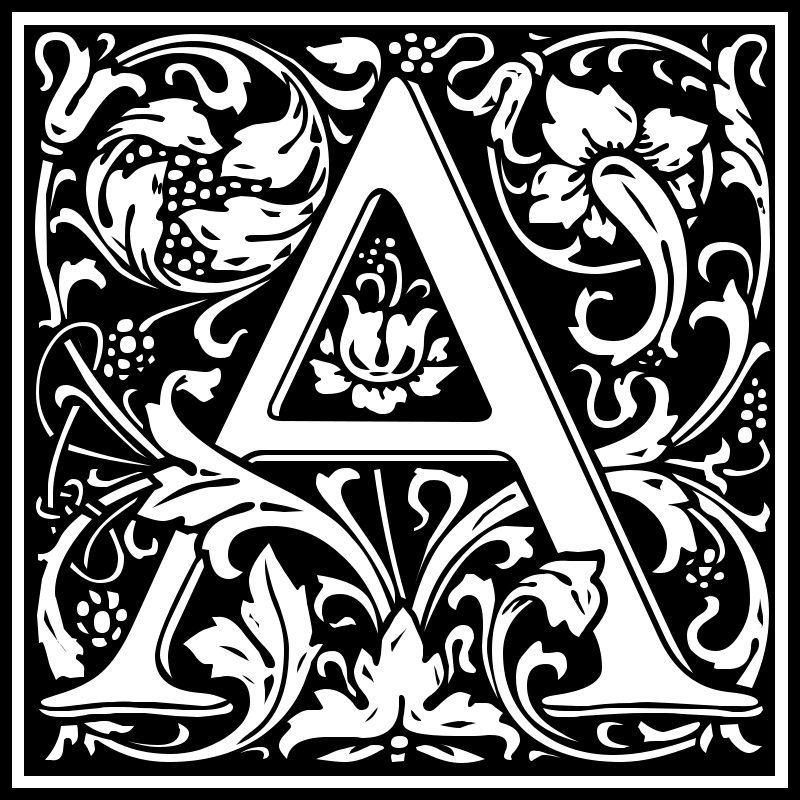
\includegraphics[width=7.5cm]{./lainicial.png}
\end{center}
\begin{description}
\item[aarónico ]   {\color{blue} 1.} \textit{ adj.} Perteneciente o relativo a Aarón, personaje bíblico, hermano de Moisés. 
\item[ababillarse ]   {\color{blue} 1.} \textit{ prnl.} Chile. Dicho de un animal: Enfermar de la babilla. 
\item[ababol ]   {\color{blue} 1.} \textit{ m.} Persona distraída, simple, abobada. U.\textit{ m.} en Aragón. En Navarra, u. c. rur.  {\color{blue} 2.} \textit{ m.} Alb., Ar., Mur. y Nav. amapola. 
\item[abacería ]   {\color{blue} 1.} \textit{ f.} Puesto o tienda donde se venden al por menor aceite, vinagre, legumbres secas, bacalao, etc. 
\item[abacero ]   {\color{blue} 1.} \textit{ m.} y\textit{ f.} Persona que tiene abacería. 
\item[abacial ]   {\color{blue} 1.} \textit{ adj.} Perteneciente o relativo al abad, a la abadesa o a la abadía. 
\item[abad ]   {\color{blue} 1.} \textit{ m.} Superior de un monasterio de hombres, considerado abadía.  {\color{blue} 2.} \textit{ m.} Dignidad superior de algunas colegiatas.  {\color{blue} 3.} \textit{ m.} En los antiguos cabildos de algunas catedrales, título de una dignidad, ya superior, ya de canónigo.  {\color{blue} 4.} \textit{ m.} carraleja.  {\color{blue} 5.} \textit{ m.} Hombre que usaba hábito eclesiástico o manteo, como los sacerdotes o estudiantes de las universidades.  {\color{blue} 6.} \textit{ m.} Ar. cura párroco.  {\color{blue} 7.} \textit{ m.} p. us. Título honorífico de la persona lega que por derecho de sucesión poseía alguna abadía con frutos secularizados.  {\color{blue} 8.} \textit{ m.}\textit{ desus.} Cura o beneficiado elegido por sus compañeros para presidirlos en cabildo durante cierto tiempo. \textasciitilde  comendaticio.  {\color{blue} 1.} \textit{ m.} El que, por merced papal, disfrutaba de ciertas rentas sobre una abadía, sin regirla ni residir en ella. $\star$ V. oreja de abad 
\item[abada ]   {\color{blue} 1.} \textit{ f.} rinoceronte. 
\item[abadejo ]   {\color{blue} 1.} \textit{ m.} bacalao.  {\color{blue} 2.} \textit{ m.} Nombre común a varios peces del mismo género que el bacalao.  {\color{blue} 3.} \textit{ m.} reyezuelo.  {\color{blue} 4.} \textit{ m.} carraleja.  {\color{blue} 5.} \textit{ m.} cantárida (|| insecto coleóptero).  {\color{blue} 6.} \textit{ m.} Pez del mar de las Antillas, de color oscuro y escamas pequeñas y rectangulares. 
\item[abadengo ]   {\color{blue} 1.} \textit{ adj.} Perteneciente o relativo a la dignidad o jurisdicción del abad. Tierras abadengas. Bienes abadengos.  {\color{blue} 2.} \textit{ m.} abadía (|| territorio, jurisdicción y bienes del abad o de la abadesa).  {\color{blue} 3.} \textit{ m.} Poseedor de territorio o bienes abadengos. $\star$ V. bienes de abadengo 
\item[abadernar ]   {\color{blue} 1.} \textit{ tr.} Mar. Sujetar con badernas. 
\item[abadesa ]   {\color{blue} 1.} \textit{ f.} Superiora en ciertas comunidades de religiosas. 
\item[abadiado ]   {\color{blue} 1.} \textit{ m.} Ar. abadía (|| territorio, jurisdicción y bienes del abad o de la abadesa). 
\item[abadiato ]   {\color{blue} 1.} \textit{ m.} abadía (|| territorio, jurisdicción y bienes del abad o de la abadesa). 
\item[abajadero ]   {\color{blue} 1.} \textit{ m.} cuesta (|| terreno en pendiente). 
\item[abajamiento ]   {\color{blue} 1.} \textit{ m.} Acción y efecto de abajar.  {\color{blue} 2.} \textit{ m.} ant. bajeza (|| abatimiento, humillación). 
\item[abajar ]   {\color{blue} 1.} \textit{ tr.} bajar. U. t. c.\textit{ intr.}  {\color{blue} 2.} \textit{ tr.} Veter. Cortar mucho del casco de las caballerías. 
\item[abajeño ]   {\color{blue} 1.} \textit{ adj.} Natural de El Bajío. U. t. c. s.  {\color{blue} 2.} \textit{ adj.} Perteneciente o relativo a esta región de los Estados de Guanajuato, Michoacán y Jalisco, en México.  {\color{blue} 3.} \textit{ adj.} Am. Natural o procedente de costas y tierras bajas. U. t. c. s.  {\color{blue} 4.} \textit{ adj.} rur. Arg. sureño. 
\item[abajo ]   {\color{blue} 1.} \textit{ adv.} l. Hacia lugar o parte inferior. Echaron la casa abajo Se tendió boca abajo  {\color{blue} 2.} \textit{ adv.} l. En lugar o parte inferior. Vive abajo, en el sótano  {\color{blue} 3.} \textit{ adv.} l. En lugar posterior, o que está después de otro, pero denotando situación inferior, ya efectiva, ya imaginada. Del rey abajo ninguno. U. especialmente en libros o escritos con referencia a lo que en ellos consta más adelante. El abajo firmante Véase abajo, página 72  {\color{blue} 4.} \textit{ adv.} l. En dirección a lo que está más bajo respecto de lo que está más alto. Cuesta abajo  {\color{blue} 5.} \textit{ adv.} l. U. en frases exclamativas, sin verbo, para reclamar la destitución o abolición de una autoridad, una institución, una ley, etc. ¡Abajo el dictador! \textasciitilde  de.  {\color{blue} 1.} \textit{ loc.} prepos.\textit{ desus.} Debajo de, al pie de. En muchos lugares de América, u. c.\textit{ coloq.} 
\item[abalada ] $\star$ V. harina abalada 
\item[abalar ]   {\color{blue} 1.} \textit{ tr.} Esp. occid. aballar {\color{blue} 1.}  
\item[abalaustrado ]   {\color{blue} 1.} \textit{ adj.} balaustrado. 
\item[abaldonadamente ]   {\color{blue} 1.} \textit{ adv.}\textit{ m.} ant. Con arrojo u osadía. 
\item[abaldonamiento ]   {\color{blue} 1.} \textit{ m.} ant. Atrevimiento, osadía. 
\item[abaldonar ]   {\color{blue} 1.} \textit{ tr.}\textit{ desus.} afrentar (|| ofender).  {\color{blue} 2.} \textit{ tr.} ant. envilecer.  {\color{blue} 3.} \textit{ tr.} ant. abandonar. U. en Salamanca y algunos lugares de América.  {\color{blue} 4.} \textit{ prnl.} ant. entregarse. 
\item[abaleador ]   {\color{blue} 1.} \textit{ m.} y\textit{ f.} Persona que abalea {\color{blue} 1.}  
\item[abaleadura ]   {\color{blue} 1.} \textit{ f.} Acción y efecto de abalear {\color{blue} 1.}   {\color{blue} 2.} \textit{ f.} pl. Granzas o residuos que quedan después de abalear {\color{blue} 1.}  
\item[abalear ]   {\color{blue} 1.} \textit{ tr.} Separar del trigo, cebada, etc., después de aventados, y con escoba a propósito para ello, los granzones y la paja gruesa. abalear {\color{blue} 2.}   {\color{blue} 1.} \textit{ tr.} Am. balear {\color{blue} 3.}  
\item[abaleo ]   {\color{blue} 1.} \textit{ m.} Acción de abalear {\color{blue} 1.}   {\color{blue} 2.} \textit{ m.} Escoba con que se abalea {\color{blue} 1.}   {\color{blue} 3.} \textit{ m.} Nombre común a varias plantas duras y espinosas de las que se hacen escobas para abalear {\color{blue} 1.}  abaleo {\color{blue} 2.}   {\color{blue} 1.} \textit{ m.} Col. Acción y efecto de abalear {\color{blue} 2.}  
\item[abalizamiento ]   {\color{blue} 1.} \textit{ m.} balizamiento. 
\item[abalizar ]   {\color{blue} 1.} \textit{ tr.} balizar. 
\item[aballar ]   {\color{blue} 1.} \textit{ tr.} Ast. y Sal. Mover de un lugar. U. t. c.\textit{ intr.} y c.\textit{ prnl.}  {\color{blue} 2.} \textit{ tr.}\textit{ desus.} Zarandear, sacudir.  {\color{blue} 3.} \textit{ tr.} ant. Echar abajo, abatir. U. en Salamanca. aballar {\color{blue} 2.}  (Del it. abbagliare, rebajar).  {\color{blue} 1.} \textit{ tr.} Pint. Amortiguar, desvanecer o esfumar las líneas y colores de una pintura. 
\item[aballestar ]   {\color{blue} 1.} \textit{ tr.} Mar. Tirar del medio de un cabo ya teso y sujeto por sus extremos, a fin de ponerlo más rígido, cobrando por el extremo que ha de amarrarse lo que con esta operación presta o da de sí. 
\item[abalorio ]   {\color{blue} 1.} \textit{ m.} Conjunto de cuentas agujereadas, con las cuales, ensartándolas, se hacen adornos y labores.  {\color{blue} 2.} \textit{ m.} Cada una de estas cuentas.  {\color{blue} 3.} \textit{ m.} Collar u objeto de adorno personal de poco valor. 
\item[abaluartar ]   {\color{blue} 1.} \textit{ tr.} Mil. abastionar. 
\item[abanar ]   {\color{blue} 1.} \textit{ tr.} Hacer aire con el abano.  {\color{blue} 2.} \textit{ tr.} And. y Can. Avivar la lumbre con el soplillo. 
\item[abancalar ]   {\color{blue} 1.} \textit{ tr.} Desmontar un terreno y formar bancales en él. 
\item[abanderado ]   {\color{blue} 1.} \textit{ m.} y\textit{ f.} Persona que lleva una bandera en las procesiones u otros actos públicos.  {\color{blue} 2.} \textit{ m.} y\textit{ f.} Portavoz o representante de una causa, movimiento u organización.  {\color{blue} 3.} \textit{ m.} y\textit{ f.} Oficial designado para llevar la bandera de un cuerpo de tropas que tenga concedido tal honor.  {\color{blue} 4.} \textit{ m.} Hombre que antiguamente servía al alférez para ayudarle a llevar la bandera. 
\item[abanderamiento ]   {\color{blue} 1.} \textit{ m.} Acción de abanderar. 
\item[abanderar ]   {\color{blue} 1.} \textit{ tr.} Matricular o registrar bajo la bandera de un Estado un buque de nacionalidad extranjera. U. t. c.\textit{ prnl.}  {\color{blue} 2.} \textit{ tr.} Proveer a un buque de los documentos que acreditan su bandera. U. t. c.\textit{ prnl.}  {\color{blue} 3.} \textit{ tr.} enarbolar.  {\color{blue} 4.} \textit{ tr.} Ponerse al frente de una causa, movimiento u organización.  {\color{blue} 5.} \textit{ tr.} Arg. y Chile. abanderizar. U. t. c.\textit{ prnl.}  {\color{blue} 6.} \textit{ tr.} Cuba. Entregar la bandera a una delegación deportiva o a un colectivo de trabajadores.  {\color{blue} 7.} \textit{ tr.} Méx. Entregar la bandera a un batallón o regimiento. 
\item[abanderizador ]   {\color{blue} 1.} \textit{ adj.} Que abanderiza. U. t. c. s. 
\item[abanderizar ]   {\color{blue} 1.} \textit{ tr.} Dividir en banderías. U. t. c.\textit{ prnl.} 
\item[abandonado ]   {\color{blue} 1.} \textit{ adj.} Descuidado, desidioso.  {\color{blue} 2.} \textit{ adj.} Sucio, desaseado. 
\item[abandonamiento ]   {\color{blue} 1.} \textit{ m.} p. us. abandono (|| acción de abandonar). 
\item[abandonar ]   {\color{blue} 1.} \textit{ tr.} Dejar, desamparar a alguien o algo.  {\color{blue} 2.} \textit{ tr.} Dejar una ocupación, un intento, un derecho, etc., emprendido ya. En juegos y deportes, u.\textit{ m.} c.\textit{ intr.} Al tercer asalto, abandonó.  {\color{blue} 3.} \textit{ tr.} Dejar un lugar, apartarse de él.  {\color{blue} 4.} \textit{ tr.} Cesar de frecuentar o habitar un lugar.  {\color{blue} 5.} \textit{ tr.} Apoyar, reclinar con dejadez. U.\textit{ m.} c.\textit{ prnl.}  {\color{blue} 6.} \textit{ tr.} Entregar, confiar algo a una persona o cosa. U.\textit{ m.} c.\textit{ prnl.}  {\color{blue} 7.} \textit{ prnl.} Dejarse dominar por afectos, pasiones o vicios.  {\color{blue} 8.} \textit{ prnl.} Descuidar los intereses o las obligaciones.  {\color{blue} 9.} \textit{ prnl.} Descuidar el aseo y la compostura.  {\color{blue} 10.} \textit{ prnl.} Caer de ánimo, rendirse en las adversidades y contratiempos. 
\item[abandonismo ]   {\color{blue} 1.} \textit{ m.} Tendencia a abandonar sin lucha algo que poseemos o nos corresponde. 
\item[abandonista ]   {\color{blue} 1.} \textit{ adj.} Perteneciente o relativo al abandonismo. Política abandonista.  {\color{blue} 2.} \textit{ adj.} Partidario del abandonismo. U. t. c. s. 
\item[abandono ]   {\color{blue} 1.} \textit{ m.} Acción y efecto de abandonar o abandonarse.  {\color{blue} 2.} \textit{ m.} Der. Renuncia sin beneficiario determinado, con pérdida del dominio o posesión sobre cosas que recobran su condición de bienes nullius o adquieren la de mostrencos.  {\color{blue} 3.} \textit{ m.} Der. Derecho del asegurado para exigir el pago del asegurador, dejando por cuenta de este las cosas aseguradas, a consecuencia de determinados accidentes del comercio marítimo. 
\item[abanear ]   {\color{blue} 1.} \textit{ intr.}\textit{ coloq.} vulg. Gal. oscilar (|| efectuar movimientos de vaivén). 
\item[abanicar ]   {\color{blue} 1.} \textit{ tr.} Hacer aire con el abanico. U.\textit{ m.} c.\textit{ prnl.}  {\color{blue} 2.} \textit{ tr.} Taurom. Agitar ante el toro el capote de un lado a otro.  {\color{blue} 3.} \textit{ intr.} Cuba, Nic., P. Rico y Ven. En el juego de béisbol, no darle a la pelota después de intentarlo con fuerza.  {\color{blue} 4.} \textit{ prnl.} No hacer caso, mostrar indiferencia ante algo. 
\item[abanicazo ]   {\color{blue} 1.} \textit{ m.} Golpe dado con el abanico. 
\item[abanico ]   {\color{blue} 1.} \textit{ m.} Instrumento para hacer o hacerse aire, que comúnmente tiene pie de varillas y país de tela, papel o piel, y se abre formando semicírculo.  {\color{blue} 2.} \textit{ m.} Cosa en forma de abanico, como la cola del pavo real.  {\color{blue} 3.} \textit{ m.} Serie, conjunto de diversas propuestas, opciones, etc., generalmente para elegir entre ellas.  {\color{blue} 4.} \textit{ m.} En algunas armaduras antiguas, parte lateral del codal o de la rodillera, en forma de abanico.  {\color{blue} 5.} \textit{ m.}\textit{ coloq.} Antigua cárcel modelo de Madrid, construida sobre planta de abanico. EL abanico  {\color{blue} 6.} \textit{ m.}\textit{ coloq.} sable (|| arma blanca).  {\color{blue} 7.} \textit{ m.} Mar. Especie de cabria hecha con elementos de a bordo.  {\color{blue} 8.} \textit{ m.} Cuba. Pieza de madera en forma de abanico, con una ranura arqueada en su parte media, por la que corre un listón que remata en disco y sirve, en las vías férreas, para advertir al maquinista el punto en que aquellas se bifurcan y la dirección que por allí ha de seguir el tren.  {\color{blue} 9.} \textit{ m.} Ec. soplillo (|| ruedo pequeño para avivar el fuego). en \textasciitilde .  {\color{blue} 1.} \textit{ loc.}\textit{ adv.} En forma de abanico. parecer alguien \textasciitilde  de tonta.  {\color{blue} 1.} \textit{ loc.} verb.\textit{ coloq.} p. us. Moverse mucho y sin concierto. $\star$ V. vela de abanico 
\item[abanillo ]   {\color{blue} 1.} \textit{ m.} Adorno de lienzo afollado del que se formaban ciertos cuellos alechugados.  {\color{blue} 2.} \textit{ m.}\textit{ desus.} abanico (|| para hacer aire). 
\item[abanino ]   {\color{blue} 1.} \textit{ m.}\textit{ desus.} Adorno de gasa u otra tela blanca con que ciertas damas de la corte guarnecían el escote del jubón. 
\item[abaniqueo ]   {\color{blue} 1.} \textit{ m.} Acción de abanicar o abanicarse. 
\item[abaniquería ]   {\color{blue} 1.} \textit{ f.} Fábrica o tienda de abanicos. 
\item[abaniquero ]   {\color{blue} 1.} \textit{ m.} y\textit{ f.} Persona que hace o vende abanicos. 
\item[abano ]   {\color{blue} 1.} \textit{ m.} p. us. abanico (|| para hacer aire).  {\color{blue} 2.} \textit{ m.} p. us. Aparato en forma de abanico que, colgado del techo, sirve para hacer aire. 
\item[abanto ]   {\color{blue} 1.} \textit{ adj.} Aturdido y torpe.  {\color{blue} 2.} \textit{ m.} Ave rapaz semejante al buitre, pero más pequeña, con la cabeza y cuello cubiertos de pluma, y el color blanquecino. Es muy tímida y perezosa, se alimenta de sustancias animales descompuestas, vive ordinariamente en el África septentrional y pasa en verano a Europa.  {\color{blue} 3.} \textit{ m.} Cualquier otra ave de la familia de los buitres. 
\item[abaratamiento ]   {\color{blue} 1.} \textit{ m.} Acción y efecto de abaratar. 
\item[abaratar ]   {\color{blue} 1.} \textit{ tr.} Disminuir o bajar el precio de algo, hacerlo barato o más barato. U. t. c.\textit{ prnl.} 
\item[abarbechar ]   {\color{blue} 1.} \textit{ tr.} barbechar. 
\item[abarca ]   {\color{blue} 1.} \textit{ f.} Calzado de cuero crudo que cubre solo la planta de los pies, con reborde en torno, y se asegura con cuerdas o correas sobre el empeine y el tobillo. Se hace también de caucho.  {\color{blue} 2.} \textit{ f.} Cantb. y Pal. zueco (|| zapato de madera). 
\item[abarcado ]   {\color{blue} 1.} \textit{ adj.} Calzado con abarcas. 
\item[abarcador ]   {\color{blue} 1.} \textit{ adj.} Que abarca. U. t. c. s. 
\item[abarcadura ]   {\color{blue} 1.} \textit{ f.} Acción y efecto de abarcar. 
\item[abarcamiento ]   {\color{blue} 1.} \textit{ m.} abarcadura. 
\item[abarcar ]   {\color{blue} 1.} \textit{ tr.} Ceñir algo con los brazos o con la mano.  {\color{blue} 2.} \textit{ tr.} Rodear, comprender.  {\color{blue} 3.} \textit{ tr.} Contener, implicar o encerrar en sí.  {\color{blue} 4.} \textit{ tr.} Percibir o dominar con la vista, de una vez, algo en su totalidad.  {\color{blue} 5.} \textit{ tr.} Tomar alguien a su cargo muchas cosas o negocios a un tiempo.  {\color{blue} 6.} \textit{ tr.} Cineg. Rodear un trozo de monte en que se supone que está la caza.  {\color{blue} 7.} \textit{ tr.} Am. acaparar.  {\color{blue} 8.} \textit{ tr.} Ec. Dicho de una gallina: Empollar los huevos. 
\item[abarcón ]   {\color{blue} 1.} \textit{ m.} En los coches antiguos, aro de hierro que afianzaba la lanza dentro de la punta de la tijera. 
\item[abarcuzar ]   {\color{blue} 1.} \textit{ tr.} abarcar (|| tomar a cargo muchas cosas).  {\color{blue} 2.} \textit{ tr.} León, Sal. y Zam. abarcar (|| ceñir con los brazos).  {\color{blue} 3.} \textit{ tr.} León, Sal. y Zam. abarcar (|| rodear).  {\color{blue} 4.} \textit{ tr.} rur. y vulg. Sal. Ansiar, codiciar. 
\item[abaritonado ]   {\color{blue} 1.} \textit{ adj.} Dicho de la voz: Parecida a la del barítono.  {\color{blue} 2.} \textit{ adj.} Dicho de un instrumento: Cuyo sonido tiene timbre semejante al de la voz del barítono. 
\item[abarloar ]   {\color{blue} 1.} \textit{ tr.} Mar. Situar un buque de tal suerte que su costado esté casi en contacto con el de otro buque, o con una batería, muelle, etc. U. t. c.\textit{ prnl.} 
\item[abarquero ]   {\color{blue} 1.} \textit{ m.} y\textit{ f.} Persona que hace o vende abarcas. 
\item[abarquillado ]   {\color{blue} 1.} \textit{ adj.} De forma de barquillo. 
\item[abarquillamiento ]   {\color{blue} 1.} \textit{ m.} Acción y efecto de abarquillar. 
\item[abarquillar ]   {\color{blue} 1.} \textit{ tr.} Dar a una cosa delgada, como una lámina, una plancha, un papel, etc., forma de barquillo, alabeada o enrollada. U. t. c.\textit{ prnl.} 
\item[abarracar ]   {\color{blue} 1.} \textit{ intr.} Mil. p. us. Acampar en chozas o barracas. U. t. c.\textit{ prnl.} 
\item[abarrado ]   {\color{blue} 1.} \textit{ adj.} Dicho de un paño: barrado (|| que saca alguna lista). 
\item[abarraganamiento ]   {\color{blue} 1.} \textit{ m.} amancebamiento. 
\item[abarraganarse ]   {\color{blue} 1.} \textit{ prnl.} amancebarse. 
\item[abarrajar ]   {\color{blue} 1.} \textit{ tr.} atropellar.  {\color{blue} 2.} \textit{ prnl.} Perú. encanallarse. 
\item[abarramiento ]   {\color{blue} 1.} \textit{ m.}\textit{ desus.} Acción y efecto de abarrar. 
\item[abarrancadero ]   {\color{blue} 1.} \textit{ m.} Sitio donde es fácil abarrancarse.  {\color{blue} 2.} \textit{ m.} Negocio o lance de que no se puede salir fácilmente. 
\item[abarrancamiento ]   {\color{blue} 1.} \textit{ m.} Acción y efecto de abarrancar o abarrancarse. 
\item[abarrancar ]   {\color{blue} 1.} \textit{ tr.} Dicho de la erosión o de la acción de los elementos: Formar barrancos en un terreno.  {\color{blue} 2.} \textit{ tr.} Meter en un barranco. U. t. c.\textit{ prnl.}  {\color{blue} 3.} \textit{ intr.} varar (|| encallar una embarcación). U. t. c.\textit{ prnl.}  {\color{blue} 4.} \textit{ prnl.} Meterse en negocio o lance del que no se puede salir fácilmente. 
\item[abarrar ]   {\color{blue} 1.} \textit{ tr.}\textit{ desus.} Arrojar, tirar violentamente algo.  {\color{blue} 2.} \textit{ tr.}\textit{ desus.} Golpear, apalear. 
\item[abarraz ]   {\color{blue} 1.} \textit{ m.} p. us. estafisagria. 
\item[abarredera ]   {\color{blue} 1.} \textit{ f.} ant. barredera.  {\color{blue} 2.} \textit{ f.} pl. Alb. Ganchos para sacar de los pozos cubos o latas. 
\item[abarrenar ]   {\color{blue} 1.} \textit{ tr.}\textit{ desus.} barrenar. 
\item[abarrer ]   {\color{blue} 1.} \textit{ tr.}\textit{ desus.} barrer (|| llevárselo todo). 
\item[abarrisco ]   {\color{blue} 1.} \textit{ adv.}\textit{ m.} a barrisco. 
\item[abarrotar ]   {\color{blue} 1.} \textit{ tr.} Apretar o fortalecer con barrotes algo.  {\color{blue} 2.} \textit{ tr.} Llenar completamente, atestar de géneros u otras cosas una tienda, un almacén, etc.  {\color{blue} 3.} \textit{ tr.} Llenar un espacio de personas o cosas.  {\color{blue} 4.} \textit{ tr.} Mar. Asegurar la estiba con abarrotes.  {\color{blue} 5.} \textit{ tr.} Mar. Cargar un buque aprovechando hasta los sitios más pequeños de su bodega y cámaras, y a veces parte de su cubierta.  {\color{blue} 6.} \textit{ tr.} Am. Saturar de productos el mercado, de manera que se deprecian por su excesiva abundancia. 
\item[abarrote ]   {\color{blue} 1.} \textit{ m.} Mar. Fardo pequeño o cuña que sirve para apretar la estiba, llenando sus huecos.  {\color{blue} 2.} \textit{ m.} pl. Am. Artículos para el abasto.  {\color{blue} 3.} \textit{ m.} pl. Col., Ec. y Perú. pulpería. 
\item[abarrotero ]   {\color{blue} 1.} \textit{ m.} y\textit{ f.} Bol., Col., Ec. y Méx. Persona que tiene tienda o despacho de abarrotes. 
\item[abarse ]   {\color{blue} 1.} \textit{ prnl.} defect. Apartarse, quitarse del paso, dejar libre el camino. MORF. U. en infinit. y en imper. 
\item[abastadamente ]   {\color{blue} 1.} \textit{ adv.}\textit{ m.}\textit{ desus.} Abundante o copiosamente. 
\item[abastamiento ]   {\color{blue} 1.} \textit{ m.}\textit{ desus.} abastecimiento. 
\item[abastante ]   {\color{blue} 1.} \textit{ adj.}\textit{ desus.} Bastante o suficiente. 
\item[abastanza ]   {\color{blue} 1.} \textit{ f.}\textit{ desus.} copia (|| abundancia).  {\color{blue} 2.} \textit{ adv.} c.\textit{ desus.} bastantemente. 
\item[abastar ]   {\color{blue} 1.} \textit{ tr.} abastecer. U. t. c.\textit{ prnl.}  {\color{blue} 2.} \textit{ intr.}\textit{ desus.} bastar (|| ser suficiente). U. c. dialect.  {\color{blue} 3.} \textit{ prnl.}\textit{ desus.} Satisfacerse o contentarse. 
\item[abastardar ]   {\color{blue} 1.} \textit{ intr.} bastardear. 
\item[abastecedor ]   {\color{blue} 1.} \textit{ adj.} Que abastece. U. t. c. s.  {\color{blue} 2.} \textit{ m.} C. Rica. Tienda de comestibles y otros enseres de uso doméstico. 
\item[abastecer ]   {\color{blue} 1.} \textit{ tr.} Proveer de bastimentos, víveres u otras cosas necesarias. U. t. c.\textit{ prnl.} MORF. conjug. c. agradecer. 
\item[abastecimiento ]   {\color{blue} 1.} \textit{ m.} Acción y efecto de abastecer. $\star$ V. libreta de abastecimientos 
\item[abastero ]   {\color{blue} 1.} \textit{ m.} Chile. Comprador de reses vivas, destinadas al matadero. 
\item[abastimiento ]   {\color{blue} 1.} \textit{ m.}\textit{ desus.} abastecimiento. 
\item[abastionar ]   {\color{blue} 1.} \textit{ tr.} Mil. Fortificar con bastiones. 
\item[abasto ]   {\color{blue} 1.} \textit{ m.} Provisión de bastimentos, y especialmente de víveres. U. t. en pl. con el mismo significado que en sing.  {\color{blue} 2.} \textit{ m.} abundancia.  {\color{blue} 3.} \textit{ m.} En el arte del bordado, pieza o piezas menos principales de la obra.  {\color{blue} 4.} \textit{ m.} Ven. Tienda pequeña de comestibles. U. t. en pl. con el mismo significado que en sing.  {\color{blue} 5.} \textit{ adv.}\textit{ m.}\textit{ desus.} Copiosa o abundantemente. dar \textasciitilde .  {\color{blue} 1.} \textit{ loc.} verb. Dar o ser bastante, bastar, proveer suficientemente. U.\textit{ m.} con neg. $\star$ V. plaza de abastos 
\item[abatanar ]   {\color{blue} 1.} \textit{ tr.} Batir o golpear el paño en el batán para desengrasarlo y enfurtirlo.  {\color{blue} 2.} \textit{ tr.} p. us. Batir o golpear de otro modo, maltratar.  {\color{blue} 3.} \textit{ prnl.} NO Arg. y Bol. p. us. Dicho de un tejido: Desgastarse, apelmazarse por el uso o el lavado. 
\item[abate ]   {\color{blue} 1.} \textit{ m.} Eclesiástico de órdenes menores, y a veces simple tonsurado, que solía vestir traje clerical a la romana.  {\color{blue} 2.} \textit{ m.} Presbítero extranjero, especialmente francés o italiano, y también eclesiástico español que ha residido mucho tiempo en Francia o Italia.  {\color{blue} 3.} \textit{ m.} Clérigo dieciochesco frívolo y cortesano. 
\item[abatidero ]   {\color{blue} 1.} \textit{ m.} Cauce de desagüe. 
\item[abatido ]   {\color{blue} 1.} \textit{ adj.} Abyecto, ruin, despreciable.  {\color{blue} 2.} \textit{ adj.} Dicho de una mercancía: Que ha caído de su estimación y precio regular. 
\item[abatidura ]   {\color{blue} 1.} \textit{ f.} ant. Acción de abatirse (|| descender el ave). 
\item[abatimiento ]   {\color{blue} 1.} \textit{ m.} Acción y efecto de abatir o abatirse.  {\color{blue} 2.} \textit{ m.} Humillación, afrenta o bajeza.  {\color{blue} 3.} \textit{ m.} Postración física o moral de una persona.  {\color{blue} 4.} \textit{ m.} Mar. Ángulo que forma la línea de la quilla con la dirección que realmente sigue la nave.  {\color{blue} 5.} \textit{ m.}\textit{ desus.} Persona o cosa afrentosa. 
\item[abatir ]   {\color{blue} 1.} \textit{ tr.} Derribar, derrocar, echar por tierra. U. t. c.\textit{ prnl.}  {\color{blue} 2.} \textit{ tr.} Hacer que algo caiga o descienda. Abatir las velas de una embarcación. U. t. en sent. fig. Roma abatió el poder de Cartago.  {\color{blue} 3.} \textit{ tr.} Inclinar, tumbar, poner tendido lo que estaba vertical. Abatir los palos de un buque, la chimenea de un vapor.  {\color{blue} 4.} \textit{ tr.} humillar. U. t. c.\textit{ prnl.}  {\color{blue} 5.} \textit{ tr.} Hacer perder el ánimo, las fuerzas, el vigor. U.\textit{ m.} c.\textit{ prnl.}  {\color{blue} 6.} \textit{ tr.} Desarmar o descomponer algo, especialmente una tienda de campaña y, en la Marina, la pipería y los camarotes.  {\color{blue} 7.} \textit{ tr.} Dicho de un jugador: En determinados juegos de naipes, conseguir la jugada máxima y descubrir sus cartas, generalmente en forma de abanico sobre la mesa.  {\color{blue} 8.} \textit{ tr.} Geom. Hacer girar alrededor de su traza un plano secante a otro, hasta superponerlo a este. U. t. c.\textit{ prnl.}  {\color{blue} 9.} \textit{ intr.} Mar. Dicho de un buque: Desviarse de su rumbo a impulso del viento o de una corriente.  {\color{blue} 10.} \textit{ prnl.} Dicho de un ave, de un avión, etc.: Descender, precipitarse a tierra o sobre una presa. El cuervo se abatió sobre una peña. Los bombarderos se abatían sobre la población. U. t. en sent. fig. La desgracia se abatió sobre mí. 
\item[abatismo ]   {\color{blue} 1.} \textit{ m.} p. us. Poder de los abates.  {\color{blue} 2.} \textit{ m.} p. us. Conjunto de abates. 
\item[abatojar ]   {\color{blue} 1.} \textit{ tr.} Ar. Batir las alubias u otras legumbres después de secas, para que las vainas suelten el grano. 
\item[abayado ]   {\color{blue} 1.} \textit{ adj.} Bot. Parecido a la baya.  {\color{blue} 2.} \textit{ adj.} R. Dom. Agotado por el calor excesivo o por un trabajo duro. 
\item[abazón ]   {\color{blue} 1.} \textit{ m.} Zool. Cada uno de los dos sacos o bolsas que dentro de la boca tienen muchos monos y algunos roedores, para depositar los alimentos antes de masticarlos. 
\item[abderitano ]   {\color{blue} 1.} \textit{ adj.} Natural de Abdera, hoy Adra, en España. U. t. c. s.  {\color{blue} 2.} \textit{ adj.} Natural de Abdera, hoy Balastra, en Tracia.  {\color{blue} 3.} \textit{ adj.} Perteneciente o relativo a alguna de estas dos antiguas ciudades. 
\item[abdicación ]   {\color{blue} 1.} \textit{ f.} Acción y efecto de abdicar.  {\color{blue} 2.} \textit{ f.} Documento en que consta la abdicación. 
\item[abdicar ]   {\color{blue} 1.} \textit{ tr.} Dicho de un rey o de un príncipe: Ceder su soberanía o renunciar a ella. U. t. en sent. fig.  {\color{blue} 2.} \textit{ tr.} Renunciar a derechos, ventajas, opiniones, etc., o cederlos.  {\color{blue} 3.} \textit{ tr.}\textit{ desus.} Privar a alguien de un estado favorable, de un derecho, facultad o poder. 
\item[abdicativamente ]   {\color{blue} 1.} \textit{ adv.}\textit{ m.} Por delegación. 
\item[abdicativo ]   {\color{blue} 1.} \textit{ adj.} Perteneciente o relativo a la abdicación. 
\item[abdomen ]   {\color{blue} 1.} \textit{ m.} Anat. vientre (|| cavidad del cuerpo de los vertebrados). En los mamíferos queda limitada por el diafragma.  {\color{blue} 2.} \textit{ m.} Anat. vientre (|| conjunto de vísceras).  {\color{blue} 3.} \textit{ m.} Zool. En muchos animales invertebrados, región que sigue al tórax; p. ej., en los insectos.  {\color{blue} 4.} \textit{ m.} Adiposidad, gordura.  {\color{blue} 5.} \textit{ m.} Vientre del hombre o de la mujer, en especial cuando es prominente. 
\item[abdominal ]   {\color{blue} 1.} \textit{ adj.} Perteneciente o relativo al abdomen. Extremidades abdominales $\star$ V. aleta abdominal aorta abdominal tifus abdominal 
\item[abducción ]   {\color{blue} 1.} \textit{ f.} Movimiento por el cual un miembro u otro órgano se aleja del plano medio que divide imaginariamente el cuerpo en dos partes simétricas. Abducción del brazo, del ojo.  {\color{blue} 2.} \textit{ f.} Supuesto secuestro de seres humanos, llevado a cabo por criaturas extraterrestres, con objeto de someterlos a experimentos diversos en el interior de sus naves espaciales.  {\color{blue} 3.} \textit{ f.} Fil. Silogismo cuya premisa mayor es evidente y la menor menos evidente o solo probable. 
\item[abductor ]   {\color{blue} 1.} \textit{ adj.} Capaz de ejecutar una abducción. U. t. c. s. 
\item[abecé ]   {\color{blue} 1.} \textit{ m.} abecedario (|| serie de las letras de un idioma).  {\color{blue} 2.} \textit{ m.} abecedario (|| cartel o libro para enseñar a leer).  {\color{blue} 3.} \textit{ m.} Rudimentos o principios de una ciencia o facultad, o de cualquier otro orden de conocimientos. no entender, o no saber, el \textasciitilde .  {\color{blue} 1.}  locs. verbs. coloqs. Ser muy ignorante. 
\item[abecedario ]   {\color{blue} 1.} \textit{ m.} Serie de las letras de un idioma, según el orden en que cada uno de ellos las considera colocadas.  {\color{blue} 2.} \textit{ m.} Cartel o libro con las letras del abecedario, que sirve para enseñar a leer.  {\color{blue} 3.} \textit{ m.} Orden alfabético.  {\color{blue} 4.} \textit{ m.} Lista en orden alfabético.  {\color{blue} 5.} \textit{ m.} abecé (|| rudimentos o principios).  {\color{blue} 6.} \textit{ m.} Impr. Orden de las signaturas de los pliegos de una impresión cuando van señalados con letras. \textasciitilde  manual.  {\color{blue} 1.} \textit{ m.} Sistema de signos que en equivalencia de las letras del alfabeto se hacen con los dedos de la mano, y que usan principalmente los sordomudos para comunicarse entre sí o con otras personas. \textasciitilde  telegráfico.  {\color{blue} 1.} \textit{ m.} Conjunto de signos o cifras que se emplean en la telegrafía. 
\item[abedul ]   {\color{blue} 1.} \textit{ m.} Árbol de la familia de las Betuláceas, de unos diez metros de altura, con hojas pequeñas, puntiagudas y doblemente aserradas o dentadas, y dispuestas en ramillas colgantes que forman una copa de forma irregular que da escasa sombra. Abunda en los montes de Europa, y su corteza, que contiene un aceite esencial, se usa para curtir y aromatizar la piel de Rusia.  {\color{blue} 2.} \textit{ m.} Madera de este árbol. 
\item[abeja ]   {\color{blue} 1.} \textit{ f.} Insecto himenóptero, de unos quince milímetros de largo, de color pardo negruzco y con vello rojizo. Vive en colonias, cada una de las cuales consta de una sola hembra fecunda, muchos machos y numerosísimas hembras estériles; habita en los huecos de los árboles o de las peñas, o en las colmenas que el hombre le prepara, y produce la cera y la miel.  {\color{blue} 2.} \textit{ f.} Persona laboriosa y previsora. \textasciitilde  albañila.  {\color{blue} 1.} \textit{ f.} Insecto himenóptero que vive apareado y hace para su morada agujeros horizontales en las tapias y en los terrenos duros. \textasciitilde  carpintera.  {\color{blue} 1.}  (Porque fabrica su panal en los troncos secos de los árboles).\textit{ f.} Himenóptero del tamaño y forma del abejorro, y de color negro morado, común en España. \textasciitilde  machiega.  {\color{blue} 1.} \textit{ f.} abeja neutra. \textasciitilde  maesa, o \textasciitilde  maestra.  {\color{blue} 1.} \textit{ f.} Hembra fecunda de las abejas, única en cada colmena. \textasciitilde  neutra, o \textasciitilde  obrera.  {\color{blue} 1.} \textit{ f.} Cada una de las que carecen de la facultad de procrear y producen la cera y la miel. \textasciitilde  reina.  {\color{blue} 1.} \textit{ f.} abeja maesa. $\star$ V. flor de la abeja nido de abeja 
\item[abejar ]   {\color{blue} 1.} \textit{ m.} colmenar. $\star$ V. uva abejar 
\item[abejarrón ]   {\color{blue} 1.} \textit{ m.} abejorro (|| insecto himenóptero).  {\color{blue} 2.} \textit{ m.} Juego entre tres personas, una de las cuales, puesta en medio con las manos juntas delante de la boca, hace un ruido semejante al del abejón, y entreteniendo así a las otras dos, procura darles bofetadas y evitar las de ellas. 
\item[abejaruco ]   {\color{blue} 1.} \textit{ m.} Pájaro del suborden de los Sindáctilos, de unos quince centímetros de longitud, con alas puntiagudas y largas y pico algo curvo, más largo que la cabeza. En su plumaje, de vistoso colorido, dominan el amarillo, el verde y el rojo oscuro. Abunda en España y es perjudicial para los colmenares, porque se come las abejas.  {\color{blue} 2.} \textit{ m.} p. us. Persona noticiera o chismosa. 
\item[abejero ]   {\color{blue} 1.} \textit{ m.} y\textit{ f.} colmenero (|| persona que cuida de las colmenas).  {\color{blue} 2.} \textit{ m.} abejaruco (|| pájaro).  {\color{blue} 3.} \textit{ f.} colmenar.  {\color{blue} 4.} \textit{ f.} toronjil. 
\item[abejón ]   {\color{blue} 1.} \textit{ m.} zángano.  {\color{blue} 2.} \textit{ m.} abejorro (|| insecto himenóptero).  {\color{blue} 3.} \textit{ m.} escarabajo sanjuanero.  {\color{blue} 4.} \textit{ m.} C. Rica y Hond. Nombre genérico de varias especies de escarabajo.  {\color{blue} 5.} \textit{ m.}\textit{ desus.} abejarrón (|| juego). jugar al \textasciitilde  con alguien.  {\color{blue} 1.} \textit{ loc.} verb.\textit{ coloq.} p. us. Tenerle en poco, tratarle con desprecio, burlarse de él. 
\item[abejorreo ]   {\color{blue} 1.} \textit{ m.} Zumbido de las abejas y otros insectos semejantes.  {\color{blue} 2.} \textit{ m.} Rumor confuso de voces o conversaciones. 
\item[abejorro ]   {\color{blue} 1.} \textit{ m.} Insecto himenóptero, de dos a tres centímetros de largo, velludo y con la trompa casi de la misma longitud que el cuerpo. Vive en enjambres poco numerosos, hace el nido debajo del musgo o de piedras y zumba mucho al volar.  {\color{blue} 2.} \textit{ m.} escarabajo sanjuanero.  {\color{blue} 3.} \textit{ m.} Persona de conversación pesada y molesta. 
\item[abejuno ]   {\color{blue} 1.} \textit{ adj.}\textit{ desus.} Perteneciente o relativo a la abeja. 
\item[abellacado ]   {\color{blue} 1.} \textit{ adj.} Bellaco, vil. 
\item[abellacar ]   {\color{blue} 1.} \textit{ tr.} Hacer bellaco, envilecer. U.\textit{ m.} c.\textit{ prnl.} 
\item[abellota ]   {\color{blue} 1.} \textit{ f.} rur. bellota (|| fruto de la encina). 
\item[abellotado ]   {\color{blue} 1.} \textit{ adj.} De forma parecida a la de la bellota. 
\item[abelmosco ]   {\color{blue} 1.} \textit{ m.} Planta de la familia de las Malváceas, con tallo peludo y hojas acorazonadas, angulosas, puntiagudas y aserradas. Procede de la India, y sus semillas, de olor almizcleño, se emplean en medicina y perfumería. 
\item[abemoladamente ]   {\color{blue} 1.} \textit{ adv.}\textit{ m.} dulcemente. 
\item[abemolar ]   {\color{blue} 1.} \textit{ tr.} Poner bemoles.  {\color{blue} 2.} \textit{ tr.} Suavizar, dulcificar la voz. 
\item[abencerraje ]   {\color{blue} 1.} \textit{ com.} Individuo de una familia del reino musulmán granadino del siglo XV, rival de la de los zegríes. $\star$ V. zegríes y abencerrajes 
\item[abenuz ]   {\color{blue} 1.} \textit{ m.} ébano. 
\item[aberenjenado ]   {\color{blue} 1.} \textit{ adj.} De color o forma del fruto de la berenjena. 
\item[aberración ]   {\color{blue} 1.} \textit{ f.} Grave error del entendimiento.  {\color{blue} 2.} \textit{ f.} Acto o conducta depravados, perversos, o que se apartan de lo aceptado como lícito.  {\color{blue} 3.} \textit{ f.} Astr. Desvío aparente de los astros, resultante de la combinación de la velocidad de la luz con la de los movimientos de la Tierra.  {\color{blue} 4.} \textit{ f.} Biol. Desviación del tipo normal que en determinados casos experimenta un carácter morfológico o fisiológico.  {\color{blue} 5.} \textit{ f.} Ópt. Imperfección de un sistema óptico que produce una imagen defectuosa. \textasciitilde  cromática.  {\color{blue} 1.} \textit{ f.} Fís. Defecto de un sistema óptico al no coincidir las imágenes de un mismo objeto producidas por los diferentes colores de la luz. \textasciitilde  de esfericidad.  {\color{blue} 1.} \textit{ f.} Ópt. Imperfección que presentan algunas imágenes producidas por sistemas ópticos al no corresponder a cada punto o recta del objeto un punto o recta, respectivamente, de la imagen. 
\item[aberrar ]   {\color{blue} 1.} \textit{ intr.} Desviarse, extraviarse, apartarse de lo normal o usual. 
\item[abertal ]   {\color{blue} 1.} \textit{ adj.} Dicho de una finca rústica o de un campo: Que no está cerrado con tapia, vallado ni de otra manera.  {\color{blue} 2.} \textit{ adj.} Dicho de un terreno: Que con la sequía se agrieta. $\star$ V. tierra abertal 
\item[abertura ]   {\color{blue} 1.} \textit{ f.} Acción de abrir o abrirse.  {\color{blue} 2.} \textit{ f.} Boca, hendidura, agujero.  {\color{blue} 3.} \textit{ f.} grieta (|| hendidura en la tierra).  {\color{blue} 4.} \textit{ f.} Terreno ancho y abierto que media entre dos montañas.  {\color{blue} 5.} \textit{ f.} ensenada (|| parte de mar que entra en la tierra).  {\color{blue} 6.} \textit{ f.} Der. apertura (|| de un testamento).  {\color{blue} 7.} \textit{ f.} Fon. Amplitud que los órganos articulatorios dejan al paso del aire, cuando se emite un sonido.  {\color{blue} 8.} \textit{ f.} Fon. Cualidad que el sonido recibe según sea la amplitud que los órganos articulatorios dejan al paso del aire, cuando es emitido.  {\color{blue} 9.} \textit{ f.} Ópt. apertura (|| diámetro de la lente).  {\color{blue} 10.} \textit{ f.} p. us. Franqueza, lisura en el trato y conversación. 
\item[abesana ]   {\color{blue} 1.} \textit{ f.}\textit{ desus.} besana (|| labor). 
\item[abesón ]   {\color{blue} 1.} \textit{ m.} eneldo. 
\item[abestiado ]   {\color{blue} 1.} \textit{ adj.} Que parece bestia.  {\color{blue} 2.} \textit{ adj.} De bestia. 
\item[abestializado ]   {\color{blue} 1.} \textit{ adj.} abestiado. 
\item[abéstola ]   {\color{blue} 1.} \textit{ f.} aguijada (|| del arado). 
\item[abetal ]   {\color{blue} 1.} \textit{ m.} Sitio poblado de abetos. 
\item[abetar ]   {\color{blue} 1.} \textit{ m.} abetal. 
\item[abete ]   {\color{blue} 1.} \textit{ m.}\textit{ desus.} abeto. U. en el Alto Aragón. abete {\color{blue} 2.}  (De or. inc.; cf. fr. happe, grapa, laña, neerl. happ, morder).  {\color{blue} 1.} \textit{ m.} Hierro pequeño, con un gancho en cada extremidad, que sirve para asegurar en el tablero la parte de paño que se tunde de una vez. 
\item[abetinote ]   {\color{blue} 1.} \textit{ m.} Resina líquida que fluye a través de la corteza del abeto o pinabete, donde suele condensarse. 
\item[abeto ]   {\color{blue} 1.} \textit{ m.} Árbol de la familia de las Abietáceas, que llega hasta 50 m de altura, con tronco alto y derecho, de corteza blanquecina, copa cónica de ramas horizontales, hojas aciculares y persistentes, flores poco visibles y fruto en piñas casi cilíndricas. Crece en parajes frescos y elevados, forma bosques en los Pirineos españoles, y su madera, no muy resistente, se aprecia, por su tamaño y blancura, para determinadas construcciones.  {\color{blue} 2.} \textit{ m.} Madera de cualquiera de las especies de este árbol. \textasciitilde  blanco.  {\color{blue} 1.} \textit{ m.} abeto (|| árbol abietáceo). \textasciitilde  del norte, \textasciitilde  falso, o \textasciitilde  rojo.  {\color{blue} 1.} \textit{ m.} pícea. $\star$ V. aceite de abeto 
\item[abetuna ]   {\color{blue} 1.} \textit{ f.} Hues. Pimpollo del abeto común. 
\item[abetunado ]   {\color{blue} 1.} \textit{ adj.} Semejante al betún en alguna de sus cualidades. 
\item[abetunar ]   {\color{blue} 1.} \textit{ tr.}\textit{ desus.} embetunar. 
\item[abey ]   {\color{blue} 1.} \textit{ m.} Árbol leguminoso de las Antillas, de unos 20 m de altura, con hojas alternas y ovaladas, que sirven para el mantenimiento de los ganados, y cuya madera, fuerte y muy compacta, se usa en carpintería. \textasciitilde  hembra.  {\color{blue} 1.} \textit{ m.} abey. \textasciitilde  macho.  {\color{blue} 1.} \textit{ m.} Árbol tropical, de la familia de las Bignoniáceas, de gran altura y ramaje, con hojas compuestas, flores pequeñas y fruto capsular. Su madera se aprecia mucho para obras de torno. 
\item[abia ]   {\color{blue} 1.} \textit{ f.} vulg. Ál. arándano. 
\item[abiar ]   {\color{blue} 1.} \textit{ m.} manzanilla loca. 
\item[abibollo ]   {\color{blue} 1.} \textit{ m.}\textit{ coloq.} Ál. ababol. 
\item[abierta ]   {\color{blue} 1.} \textit{ f.} V. abierto. abierto, ta. (Del part. irreg. de abrir; lat. apĕrtus).  {\color{blue} 1.} \textit{ adj.} Dicho comúnmente del campo: Desembarazado, llano, raso, dilatado.  {\color{blue} 2.} \textit{ adj.} No murado, no cercado.  {\color{blue} 3.} \textit{ adj.} Dicho de una persona: Franca, llana, receptiva.  {\color{blue} 4.} \textit{ adj.} Dicho de una relación o de una lista: Susceptible de cambios.  {\color{blue} 5.} \textit{ adj.} Dicho de un asunto o de un negocio: No resuelto. El trato queda abierto  {\color{blue} 6.} \textit{ adj.} Dicho de una caballería: Que separa excesivamente sus extremidades al andar.  {\color{blue} 7.} \textit{ adj.} Fon. Dicho de un sonido: Que se articula con mayor grado de abertura que otro sonido que se considera cerrado. Vocal abierta  {\color{blue} 8.} \textit{ adj.} Mar. Dicho de una embarcación: Que no tiene cubierta.  {\color{blue} 9.} \textit{ adj.}\textit{ desus.} Claro, patente, indudable.  {\color{blue} 10.} \textit{ m.} Dep. Competición deportiva en la que pueden participar todas las categorías.  {\color{blue} 11.} \textit{ f.} Col. y Nic. abertura (|| acción de abrir).  {\color{blue} 12.} \textit{ f.}\textit{ desus.} abertura (|| boca, hendidura).  {\color{blue} 13.} \textit{ adv.}\textit{ m.} ant. abiertamente. en abierto.  {\color{blue} 1.} \textit{ loc.}\textit{ adj.} Dicho de una emisión televisiva: Sin codificar. Ese canal ha estrenado un nuevo programa en abierto $\star$ V. carga abierta carta abierta cartela abierta casa abierta circuito abierto concejo abierto crédito abierto curva abierta espejuela abierta guerra abierta hogar abierto jornada de puertas abiertas letra abierta línea abierta orden abierto puerta abierta resto abierto sílaba abierta testamento abierto vaca abierta vaina abierta viento abierto 
\item[abiertamente ]   {\color{blue} 1.} \textit{ adv.}\textit{ m.} Sin reserva, francamente.  {\color{blue} 2.} \textit{ adv.}\textit{ m.} Clara, patentemente. 
\item[abierto ]   {\color{blue} 1.} \textit{ adj.} Dicho comúnmente del campo: Desembarazado, llano, raso, dilatado.  {\color{blue} 2.} \textit{ adj.} No murado, no cercado.  {\color{blue} 3.} \textit{ adj.} Dicho de una persona: Franca, llana, receptiva.  {\color{blue} 4.} \textit{ adj.} Dicho de una relación o de una lista: Susceptible de cambios.  {\color{blue} 5.} \textit{ adj.} Dicho de un asunto o de un negocio: No resuelto. El trato queda abierto  {\color{blue} 6.} \textit{ adj.} Dicho de una caballería: Que separa excesivamente sus extremidades al andar.  {\color{blue} 7.} \textit{ adj.} Fon. Dicho de un sonido: Que se articula con mayor grado de abertura que otro sonido que se considera cerrado. Vocal abierta  {\color{blue} 8.} \textit{ adj.} Mar. Dicho de una embarcación: Que no tiene cubierta.  {\color{blue} 9.} \textit{ adj.}\textit{ desus.} Claro, patente, indudable.  {\color{blue} 10.} \textit{ m.} Dep. Competición deportiva en la que pueden participar todas las categorías.  {\color{blue} 11.} \textit{ f.} Col. y Nic. abertura (|| acción de abrir).  {\color{blue} 12.} \textit{ f.}\textit{ desus.} abertura (|| boca, hendidura).  {\color{blue} 13.} \textit{ adv.}\textit{ m.} ant. abiertamente. en abierto.  {\color{blue} 1.} \textit{ loc.}\textit{ adj.} Dicho de una emisión televisiva: Sin codificar. Ese canal ha estrenado un nuevo programa en abierto $\star$ V. carga abierta carta abierta cartela abierta casa abierta circuito abierto concejo abierto crédito abierto curva abierta espejuela abierta guerra abierta hogar abierto jornada de puertas abiertas letra abierta línea abierta orden abierto puerta abierta resto abierto sílaba abierta testamento abierto vaca abierta vaina abierta viento abierto 
\item[abietáceo ]   {\color{blue} 1.} \textit{ adj.} Bot. Se dice de los árboles gimnospermos bastante ramificados, con hojas persistentes de limbo muy estrecho y aun acicular, flores unisexuales monoicas, las masculinas reunidas en amentos y las femeninas en estróbilos. Las semillas, que nunca son carnosas, están cubiertas por escamas muy apretadas; p. ej., el pino, el abeto, el alerce y el cedro. U. t. c. s.\textit{ f.}  {\color{blue} 2.} \textit{ f.} pl. Bot. Familia de estas plantas. ORTOGR. Escr. con may. inicial. 
\item[abiete ]   {\color{blue} 1.} \textit{ m.}\textit{ desus.} abeto. 
\item[abietíneo ]   {\color{blue} 1.} \textit{ adj.} Bot. abietáceo. U. t. c. s.\textit{ f.} ORTOGR. Escr. con may. inicial c. taxón. 
\item[abietino ]   {\color{blue} 1.} \textit{ adj.} Se dice de la resina del abeto.  {\color{blue} 2.} \textit{ m.} abetinote. 
\item[abigarrado ]   {\color{blue} 1.} \textit{ adj.} De varios colores, mal combinados.  {\color{blue} 2.} \textit{ adj.} Heterogéneo, reunido sin concierto. Un extraño y abigarrado libro. Una multitud abigarrada. 
\item[abigarramiento ]   {\color{blue} 1.} \textit{ m.} Acción y efecto de abigarrar.  {\color{blue} 2.} \textit{ m.} Cualidad de abigarrado. 
\item[abigarrar ]   {\color{blue} 1.} \textit{ tr.} Dar o poner a algo varios colores mal combinados.  {\color{blue} 2.} \textit{ prnl.} Dicho de cosas varias y heterogéneas: Amontonarse, apretujarse. 
\item[abigeato ]   {\color{blue} 1.} \textit{ m.} Am. Hurto de ganado. 
\item[abigeo ]   {\color{blue} 1.} \textit{ m.} Am. Ladrón de ganado. 
\item[abigotado ]   {\color{blue} 1.} \textit{ adj.} bigotudo. 
\item[abintestato ]   {\color{blue} 1.} \textit{ m.} Der. Procedimiento judicial sobre herencia y adjudicación de bienes de quien muere sin testar. 
\item[abipón ]   {\color{blue} 1.} \textit{ adj.} Se dice del individuo de un pueblo amerindio que habitaba cerca del Paraná. U. t. c. s.  {\color{blue} 2.} \textit{ adj.} Perteneciente o relativo a los abipones.  {\color{blue} 3.} \textit{ m.} Lengua de la familia guaicurú hablada por los abipones. 
\item[abisagrar ]   {\color{blue} 1.} \textit{ tr.} Clavar o fijar bisagras en las puertas y sus marcos, o en otros objetos. 
\item[abisal ]   {\color{blue} 1.} \textit{ adj.} abismal (|| perteneciente al abismo).  {\color{blue} 2.} \textit{ adj.} Se dice de las zonas del mar profundo que se extienden más allá del talud continental, y corresponden a profundidades mayores de 2000\textit{ m.}  {\color{blue} 3.} \textit{ adj.} Perteneciente o relativo a tales zonas. 
\item[abiselar ]   {\color{blue} 1.} \textit{ tr.} biselar. 
\item[abisinio ]   {\color{blue} 1.} \textit{ adj.} Natural de Abisinia, hoy Etiopía. U. t. c. s.  {\color{blue} 2.} \textit{ adj.} Perteneciente o relativo a este país de África.  {\color{blue} 3.} \textit{ m.} Lengua abisinia. $\star$ V. rito abisinio 
\item[abismado ]   {\color{blue} 1.} \textit{ adj.} Dicho de una persona, de su expresión, de su gesto, etc.: Ensimismados, reconcentrados.  {\color{blue} 2.} \textit{ adj.} Heráld. Dicho de una pieza del escudo: Puesta en el abismo. 
\item[abismal ]   {\color{blue} 1.} \textit{ m.} Cada uno de los clavos con que se fijaba en el asta el hierro de la lanza. abismal {\color{blue} 2.}   {\color{blue} 1.} \textit{ adj.} Perteneciente o relativo al abismo.  {\color{blue} 2.} \textit{ adj.} Muy profundo, insondable, incomprensible. 
\item[abismar ]   {\color{blue} 1.} \textit{ tr.} Hundir en un abismo. U. t. c.\textit{ prnl.}  {\color{blue} 2.} \textit{ tr.} Confundir, abatir. U. t. c.\textit{ prnl.}  {\color{blue} 3.} \textit{ prnl.} Entregarse del todo a la contemplación, al dolor, etc.  {\color{blue} 4.} \textit{ prnl.} Am. sorprenderse (|| conmoverse con algo imprevisto o raro). 
\item[abismático ]   {\color{blue} 1.} \textit{ adj.} abismal {\color{blue} 2.}  
\item[abismo ]   {\color{blue} 1.} \textit{ m.} Profundidad grande, imponente y peligrosa, como la de los mares, la de un tajo, la de una sima, etc. U. t. en sent. fig. Se sumió en el abismo de la desesperación.  {\color{blue} 2.} \textit{ m.} infierno (|| lugar de castigo eterno).  {\color{blue} 3.} \textit{ m.} Cosa inmensa, insondable o incomprensible.  {\color{blue} 4.} \textit{ m.} Diferencia grande entre cosas, personas, ideas, sentimientos, etc.  {\color{blue} 5.} \textit{ m.} Heráld. Punto o parte central del escudo.  {\color{blue} 6.} \textit{ m.} Nic. Maldad, perdición, ruina moral. 
\item[abiso ]   {\color{blue} 1.} \textit{ m.}\textit{ desus.} abismo. 
\item[abita ]   {\color{blue} 1.} \textit{ f.}\textit{ desus.} bita. 
\item[abitadura ]   {\color{blue} 1.} \textit{ f.} Mar. Acción de abitar. 
\item[abitaque ]   {\color{blue} 1.} \textit{ m.} cuartón (|| madero que resulta de aserrar una pieza en cruz). 
\item[abitar ]   {\color{blue} 1.} \textit{ tr.} Mar. Amarrar un cabo rodeando las bitas. 
\item[abitón ]   {\color{blue} 1.} \textit{ m.} Mar. Madero que se coloca verticalmente en un buque y sirve para amarrar o sujetar algún cabo. 
\item[abizcochado ]   {\color{blue} 1.} \textit{ adj.} Parecido al bizcocho (|| pan).  {\color{blue} 2.} \textit{ adj.} Parecido al bizcocho (|| masa). 
\item[abjuración ]   {\color{blue} 1.} \textit{ f.} Acción y efecto de abjurar. 
\item[abjurar ]   {\color{blue} 1.} \textit{ tr.} Retractarse, renegar, a veces públicamente, de una creencia o compromiso que antes se ha profesado o asumido. U. t. c.\textit{ intr.} Abjurar DE su religión. 
\item[ablación ]   {\color{blue} 1.} \textit{ f.} Acción y efecto de cortar, separar, quitar.  {\color{blue} 2.} \textit{ f.} Der. Sacrificio o menoscabo de un derecho.  {\color{blue} 3.} \textit{ f.} Med. Separación o extirpación de cualquier parte del cuerpo. \textasciitilde  continental.  {\color{blue} 1.} \textit{ f.} Geogr. Arrastre de materiales de la corteza terrestre efectuado por los ríos, los vientos, las olas, etc. \textasciitilde  glaciar.  {\color{blue} 1.} \textit{ f.} Geogr. Pérdida de hielo en el final de un glaciar. 
\item[ablandabrevas ]   {\color{blue} 1.} \textit{ com.}\textit{ coloq.} Persona inútil o pusilánime. 
\item[ablandador ]   {\color{blue} 1.} \textit{ adj.} Que ablanda. 
\item[ablandahígos ]   {\color{blue} 1.} \textit{ com.}\textit{ coloq.} ablandabrevas. 
\item[ablandamiento ]   {\color{blue} 1.} \textit{ m.} Acción y efecto de ablandar o ablandarse. 
\item[ablandar ]   {\color{blue} 1.} \textit{ tr.} Poner blando algo. U. t. c.\textit{ prnl.}  {\color{blue} 2.} \textit{ tr.} Laxar, suavizar. U. t. c.\textit{ prnl.}  {\color{blue} 3.} \textit{ tr.} Hacer que alguien ceda en una postura intransigente o severa, mitigar su ira o enojo. U. t. c.\textit{ prnl.}  {\color{blue} 4.} \textit{ tr.} Arg. y Ur. rodar (|| hacer que un automóvil marche a las velocidades prescritas para su rodaje).  {\color{blue} 5.} \textit{ intr.} Dicho del invierno: Calmar sus rigores, empezando a derretirse los hielos y las nieves.  {\color{blue} 6.} \textit{ intr.} Dicho del viento: Ceder en su fuerza. U. t. c.\textit{ prnl.}  {\color{blue} 7.} \textit{ prnl.} acobardarse. 
\item[ablandativo ]   {\color{blue} 1.} \textit{ adj.} Que tiene virtud de ablandar. 
\item[ablandecer ]   {\color{blue} 1.} \textit{ tr.}\textit{ desus.} ablandar. 
\item[ablanedo ]   {\color{blue} 1.} \textit{ m.}\textit{ coloq.} Ast. avellanar {\color{blue} 1.}  
\item[ablano ]   {\color{blue} 1.} \textit{ m.}\textit{ coloq.} Ast. avellano. 
\item[ablativo ]   {\color{blue} 1.} \textit{ m.} Gram. Caso de la declinación latina y de otras lenguas indoeuropeas, cuya función principal es expresar la procedencia local o temporal, y en latín también las relaciones de situación, tiempo, modo, instrumento, materia, etc., que en español suelen expresarse anteponiendo al nombre alguna preposición, entre las cuales son las más frecuentes bajo, con, de, desde, en, por y sin. \textasciitilde  absoluto.  {\color{blue} 1.} \textit{ m.} Gram. Clase de construcción absoluta propia del latín, caracterizada porque sus dos elementos constitutivos figuran en ablativo. Establece alguna circunstancia con respecto a la oración a la que suele preceder con autonomía fónica. ablativo2, va.  {\color{blue} 1.} \textit{ adj.} Perteneciente o relativo a la ablación. 
\item[ablegado ]   {\color{blue} 1.} \textit{ m.} Enviado apostólico encargado de entregar el birrete a los nuevos cardenales. 
\item[ablentador ]   {\color{blue} 1.} \textit{ m.}\textit{ desus.} bieldo. 
\item[ablentar ]   {\color{blue} 1.} \textit{ tr.} beldar.  {\color{blue} 2.} \textit{ tr.} aventar (|| echar al viento). ¶ MORF. conjug. c. acertar. 
\item[ablución ]   {\color{blue} 1.} \textit{ f.} lavatorio (|| acción de lavar).  {\color{blue} 2.} \textit{ f.} Acción de purificarse por medio del agua, según ritos de algunas religiones, como la judaica, la mahometana, etc.  {\color{blue} 3.} \textit{ f.} Ceremonia de purificar el cáliz y de lavarse los dedos el sacerdote después de consumir.  {\color{blue} 4.} \textit{ f.} pl. Vino y agua con que se hace esta purificación y lavatorio. Sumir las abluciones. 
\item[ablusado ]   {\color{blue} 1.} \textit{ adj.} Dicho de un corpiño: Holgado a manera de blusa. 
\item[abnegación ]   {\color{blue} 1.} \textit{ f.} Sacrificio que alguien hace de su voluntad, de sus afectos o de sus intereses, generalmente por motivos religiosos o por altruismo. 
\item[abnegado ]   {\color{blue} 1.} \textit{ adj.} Que tiene abnegación. 
\item[abnegar ]   {\color{blue} 1.} \textit{ tr.} p. us. Renunciar voluntariamente a los propios deseos, pasiones o intereses. U.\textit{ m.} c.\textit{ prnl.} MORF. conjug. c. acertar. 
\item[abobado ]   {\color{blue} 1.} \textit{ adj.} Que parece bobo.  {\color{blue} 2.} \textit{ adj.} Propio de un bobo. 
\item[abobamiento ]   {\color{blue} 1.} \textit{ m.} Acción y efecto de abobar. 
\item[abobar ]   {\color{blue} 1.} \textit{ tr.} Hacer bobo a alguien, entorpecerle el uso de las potencias. U. t. c.\textit{ prnl.}  {\color{blue} 2.} \textit{ tr.} embobar. U. t. c.\textit{ prnl.} 
\item[abobra ]   {\color{blue} 1.} \textit{ f.} Planta vivaz de la familia de las Cucurbitáceas, que se cultiva como enredadera de adorno. 
\item[abocadear ]   {\color{blue} 1.} \textit{ tr.}\textit{ desus.} Herir o maltratar a bocados.  {\color{blue} 2.} \textit{ tr.}\textit{ desus.} Tomar bocados. 
\item[abocado ]   {\color{blue} 1.} \textit{ adj.} Dicho del vino, especialmente de una clase de jerez: Que contiene mezcla de vino seco y dulce. U. t. c. s.\textit{ m.} 
\item[abocamiento ]   {\color{blue} 1.} \textit{ m.} Acción y efecto de abocar o abocarse. 
\item[abocanar ]   {\color{blue} 1.} \textit{ intr.} impers. rur. Ast. escampar (|| cesar de llover). 
\item[abocar ]   {\color{blue} 1.} \textit{ tr.} Verter el contenido de un cántaro, costal, etc., en otro. U. propiamente cuando para ello se aproximan las bocas de ambos.  {\color{blue} 2.} \textit{ tr.} Acercar, dirigir hacia un lugar armas de fuego, tropas, pertrechos, etc. U. t. c.\textit{ prnl.}  {\color{blue} 3.} \textit{ tr.}\textit{ desus.} Asir con la boca.  {\color{blue} 4.} \textit{ intr.} Desembocar, ir a parar.  {\color{blue} 5.} \textit{ intr.} Mar. Comenzar a entrar en un canal, estrecho, puerto, etc.  {\color{blue} 6.} \textit{ prnl.} Dicho de una o más personas: Juntarse de concierto con otra u otras para tratar un negocio.  {\color{blue} 7.} \textit{ prnl.} Existiendo proximidad en el tiempo, hallarse en disposición, peligro o esperanza de algo. Estar, hallarse, quedar, verse abocado A la ruptura. U. t. c.\textit{ intr.}  {\color{blue} 8.} \textit{ prnl.} Bol., C. Rica, Guat., Ur. y Ven. Entregarse de lleno a hacer algo, o dedicarse a la consideración o estudio de un asunto. La Administración se abocará A resolver los problemas de los niños. 
\item[abocardado ]   {\color{blue} 1.} \textit{ adj.} Dicho especialmente de algunas armas de fuego: De forma semejante a la de la bocina. 
\item[abocardar ]   {\color{blue} 1.} \textit{ tr.} Ensanchar la boca de un tubo o de un agujero. 
\item[abocardo ]   {\color{blue} 1.} \textit{ m.} alegra. 
\item[abocelado ]   {\color{blue} 1.} \textit{ adj.} Que tiene forma de bocel. 
\item[abocetado ]   {\color{blue} 1.} \textit{ adj.} Dicho de una pintura: Que, por estar poco concluida, más parece boceto que obra terminada. 
\item[abocetar ]   {\color{blue} 1.} \textit{ tr.} Ejecutar bocetos o dar el carácter de tales a las obras artísticas.  {\color{blue} 2.} \textit{ tr.} Insinuar, apuntar vagamente algo. 
\item[abochornado ]   {\color{blue} 1.} \textit{ adj.}\textit{ desus.} bochornoso. 
\item[abochornar ]   {\color{blue} 1.} \textit{ tr.} Dicho del excesivo calor: Causar bochorno. U. t. c.\textit{ prnl.}  {\color{blue} 2.} \textit{ tr.} sonrojar. U. t. c.\textit{ prnl.}  {\color{blue} 3.} \textit{ prnl.} Dicho de una planta: Enfermar por el excesivo calor o calma. 
\item[abocinado ]   {\color{blue} 1.} \textit{ adj.} De forma semejante a la de la bocina. $\star$ V. arco abocinado 
\item[abocinamiento ]   {\color{blue} 1.} \textit{ m.} Acción y efecto de abocinar {\color{blue} 1.}  
\item[abocinar ]   {\color{blue} 1.} \textit{ tr.} Ensanchar un tubo o cañón hacia su boca, a modo de bocina. abocinar {\color{blue} 2.}  (De or. inc.; cf. ant. abuçado, boca abajo).  {\color{blue} 1.} \textit{ intr.}\textit{ coloq.} Caer de bruces. U.\textit{ m.} c.\textit{ prnl.}  {\color{blue} 2.} \textit{ prnl.} Equit. Dicho de una caballería: Inclinarse hacia delante sobre el cuarto delantero. 
\item[abofeteador ]   {\color{blue} 1.} \textit{ adj.} Que abofetea. U. t. c. s. 
\item[abofetear ]   {\color{blue} 1.} \textit{ tr.} Dar de bofetadas.  {\color{blue} 2.} \textit{ tr.} Ultrajar, escarnecer. 
\item[abogacía ]   {\color{blue} 1.} \textit{ f.} Profesión y ejercicio del abogado.  {\color{blue} 2.} \textit{ f.} Cuerpo de abogados. 
\item[abogadesco ]   {\color{blue} 1.} \textit{ adj.} Perteneciente o relativo al abogado o a su profesión. U.\textit{ m.} en sent. despect. 
\item[abogadil ]   {\color{blue} 1.} \textit{ adj.} despect. Perteneciente o relativo a los abogados. U. en Costa Rica como no despectivo. 
\item[abogadismo ]   {\color{blue} 1.} \textit{ m.} Intervención excesiva de los abogados en los negocios públicos.  {\color{blue} 2.} \textit{ m.} Aplicación inadecuada de sus métodos a cuestiones extrañas a la abogacía. 
\item[abogado ]   {\color{blue} 1.} \textit{ m.} y\textit{ f.} Licenciado o doctor en derecho que ejerce profesionalmente la dirección y defensa de las partes en toda clase de procesos o el asesoramiento y consejo jurídico. MORF. U. t. la forma en\textit{ m.} para designar el\textit{ f.}  {\color{blue} 2.} \textit{ m.} y\textit{ f.} Intercesor o mediador.  {\color{blue} 3.} \textit{ m.} y\textit{ f.} Nic. Persona habladora, enredadora, parlanchina. abogado del diablo.  {\color{blue} 1.} \textit{ m.} Contradictor de buenas causas.  {\color{blue} 2.} \textit{ m.}\textit{ coloq.} promotor de la fe. \textasciitilde  del Estado.  {\color{blue} 1.} \textit{ m.} y\textit{ f.} Funcionario a quien se encomienda el asesoramiento, representación y defensa en juicios del Estado y sus organismos. \textasciitilde  de oficio.  {\color{blue} 1.} \textit{ m.} y\textit{ f.} Jurista asignado por el juez a una parte, ordinariamente por su falta de recursos económicos. abogado de pobres.  {\color{blue} 1.} \textit{ m.}\textit{ coloq.}\textit{ desus.} abogado de oficio. abogado de secano.  {\color{blue} 1.} \textit{ m.}\textit{ coloq.} p. us. Jurista que no ejerce ni sirve para ello.  {\color{blue} 2.} \textit{ m.}\textit{ coloq.} p. us. El que sin haber cursado la jurisprudencia entiende de leyes o presume de ello. U. en son de burla.  {\color{blue} 3.} \textit{ m.}\textit{ coloq.} p. us. El que se mete a hablar de materias en que es lego.  {\color{blue} 4.} \textit{ m.}\textit{ coloq.} p. us. Rústico avisado y diestro en el manejo de negocios superiores a su educación. abogado fiscal.  {\color{blue} 1.} \textit{ m.} Grado inferior de la carrera fiscal. \textasciitilde  general.  {\color{blue} 1.} \textit{ m.} y\textit{ f.} En los órganos judiciales de la Unión Europea, jurista que estudia la causa una vez concluida y propone al tribunal una resolución determinada. $\star$ V. barra de abogados 
\item[abogador ]   {\color{blue} 1.} \textit{ adj.} ant. Que aboga.  {\color{blue} 2.} \textit{ m.} muñidor (|| criado de cofradía). 
\item[abogamiento ]   {\color{blue} 1.} \textit{ m.} ant. Acción y efecto de abogar. 
\item[abogar ]   {\color{blue} 1.} \textit{ intr.} Defender en juicio, por escrito o de palabra.  {\color{blue} 2.} \textit{ intr.} Interceder, hablar en favor de alguien. 
\item[abohetado ]   {\color{blue} 1.} \textit{ adj.} abuhado. 
\item[abolaga ]   {\color{blue} 1.} \textit{ f.} aulaga. 
\item[abolengo ]   {\color{blue} 1.} \textit{ m.} Ascendencia de abuelos o antepasados.  {\color{blue} 2.} \textit{ m.} Ascendencia ilustre.  {\color{blue} 3.} \textit{ m.} Lugar de donde se es oriundo; nacionalidad, filiación étnica o biológica. $\star$ V. bienes de abolengo 
\item[abolición ]   {\color{blue} 1.} \textit{ f.} Acción y efecto de abolir. 
\item[abolicionismo ]   {\color{blue} 1.} \textit{ m.} Doctrina de los abolicionistas. 
\item[abolicionista ]   {\color{blue} 1.} \textit{ adj.} Dicho de una persona: Que procura dejar sin efecto o suprimir una ley, costumbre, etc. Se aplicó principalmente a los partidarios de la abolición de la esclavitud. U. t. c. s. 
\item[abolir ]   {\color{blue} 1.} \textit{ tr.} defect. Derogar, dejar sin vigencia una ley, precepto, costumbre, etc. MORF. U. solo las formas cuya desinencia empieza por -i. 
\item[abollado ]   {\color{blue} 1.} \textit{ adj.}\textit{ coloq.} Cuba. Dicho de una persona: Que se halla en mala situación económica. abollado {\color{blue} 2.}   {\color{blue} 1.} \textit{ m.}\textit{ desus.} Adorno de bollos en los metales y vestidos. 
\item[abolladura ]   {\color{blue} 1.} \textit{ f.} Acción y efecto de abollar {\color{blue} 1.}  
\item[abollar ]   {\color{blue} 1.} \textit{ tr.} Producir una depresión en una superficie con un golpe o apretándola. U. t. c.\textit{ prnl.}  {\color{blue} 2.} \textit{ tr.} Burg. hollar. abollar {\color{blue} 2.}  (De bollo1).  {\color{blue} 1.} \textit{ tr.} Adornar con bollos o relieves semiesféricos metales o telas. 
\item[abollón ]   {\color{blue} 1.} \textit{ m.} abolladura. 
\item[abollonar ]   {\color{blue} 1.} \textit{ tr.} Repujar formando bollones.  {\color{blue} 2.} \textit{ intr.} Ar. Dicho de una planta: Echar el bollón. 
\item[abolorio ]   {\color{blue} 1.} \textit{ m.} abolengo. 
\item[abolsarse ]   {\color{blue} 1.} \textit{ prnl.} Tomar forma de bolsa.  {\color{blue} 2.} \textit{ prnl.} Constr. Dicho de una pared: afollarse. 
\item[abomaso ]   {\color{blue} 1.} \textit{ m.} Zool. cuajar {\color{blue} 1.}  
\item[abombar ]   {\color{blue} 1.} \textit{ tr.} Aturdir, atolondrar, asordar. U. t. c.\textit{ prnl.}  {\color{blue} 2.} \textit{ prnl.} Dicho de un líquido o de la carne: Empezar a corromperse.  {\color{blue} 3.} \textit{ prnl.} And. y Nic. achisparse.  {\color{blue} 4.} \textit{ prnl.} Arg. Aturdirse a causa de la bebida, la comida, el calor o el cansancio. abombar {\color{blue} 2.}  (De bomba).  {\color{blue} 1.} \textit{ tr.} Dar forma convexa.  {\color{blue} 2.} \textit{ intr.} Dar a la bomba.  {\color{blue} 3.} \textit{ prnl.} Dicho de una cosa: Tomar forma convexa. 
\item[abominable ]   {\color{blue} 1.} \textit{ adj.} Digno de ser abominado.  {\color{blue} 2.} \textit{ adj.} Que desagrada profundamente. 
\item[abominación ]   {\color{blue} 1.} \textit{ f.} Acción y efecto de abominar.  {\color{blue} 2.} \textit{ f.} Cosa abominable. 
\item[abominar ]   {\color{blue} 1.} \textit{ tr.} Condenar y maldecir a alguien o algo por considerarlo malo o perjudicial. U. t. c.\textit{ intr.} Abominar DE la codicia.  {\color{blue} 2.} \textit{ tr.} aborrecer (|| tener aversión). 
\item[abonable ]   {\color{blue} 1.} \textit{ adj.} Que puede o debe ser abonado. 
\item[abonado ]   {\color{blue} 1.} \textit{ adj.} Que es de fiar por su caudal o crédito.  {\color{blue} 2.} \textit{ adj.} Dispuesto a decir o hacer algo. U.\textit{ m.} en sent. peyor.  {\color{blue} 3.} \textit{ m.} y\textit{ f.} Persona inscrita para recibir algún servicio periódicamente o determinado número de veces.  {\color{blue} 4.} \textit{ m.} y\textit{ f.} Persona que ha suscrito o adquirido un abono para un servicio o espectáculo.  {\color{blue} 5.} \textit{ m.} Acción y efecto de abonar (|| tierras laborables). abonado foliar.  {\color{blue} 1.} \textit{ m.} El que se ejecuta, los años secos, en las viñas y otras plantaciones para suministrarles, a través de las hojas, elementos fertilizantes. $\star$ V. fiador lego, llano y abonado terreno abonado 
\item[abonador ]   {\color{blue} 1.} \textit{ adj.} Que abona.  {\color{blue} 2.} \textit{ m.} y\textit{ f.} Persona que abona al fiador, y en su defecto se obliga a responder por él.  {\color{blue} 3.} \textit{ m.} Barrena de mango largo que usan los toneleros para abrir grandes taladros en las pipas.  {\color{blue} 4.} \textit{ f.} Máquina para abonar las tierras de labranza. 
\item[abonanza ]   {\color{blue} 1.} \textit{ intr.} Dicho del tiempo o de una tormenta: serenarse (|| aclararse). 
\item[abonanzar ]   {\color{blue} 1.} \textit{ intr.} Dicho del tiempo o de una tormenta: serenarse (|| aclararse). 
\item[abonar ]   {\color{blue} 1.} \textit{ tr.} Acreditar o calificar de bueno.  {\color{blue} 2.} \textit{ tr.} Salir por fiador de alguien, responder por él.  {\color{blue} 3.} \textit{ tr.} Hacer bueno o útil algo, mejorarlo de condición o estado.  {\color{blue} 4.} \textit{ tr.} Dar por cierto y seguro algo.  {\color{blue} 5.} \textit{ tr.} Echar en la tierra laborable materias que aumenten su fertilidad.  {\color{blue} 6.} \textit{ tr.} Tomar en cuenta un pago.  {\color{blue} 7.} \textit{ tr.} pagar (|| dar o satisfacer lo que se debe).  {\color{blue} 8.} \textit{ tr.} pagar (|| dar derechos los géneros).  {\color{blue} 9.} \textit{ tr.} Asentar en las cuentas corrientes las partidas que corresponden al haber.  {\color{blue} 10.} \textit{ tr.} Inscribir a alguien, mediante pago, para que pueda concurrir a alguna diversión, disfrutar de alguna comodidad o recibir algún servicio periódicamente o determinado número de veces. U.\textit{ m.} c.\textit{ prnl.}  {\color{blue} 11.} \textit{ tr.} Com. Pagar la cantidad correspondiente a cada uno de los vencimientos de una venta o un préstamo a plazos.  {\color{blue} 12.} \textit{ intr.} abonanzar.  {\color{blue} 13.} \textit{ prnl.} Insistir en un acto que agrada, desear practicarlo con reiteración. Me abonaría a veranear allí. 
\item[abondado ]   {\color{blue} 1.} \textit{ adj.}\textit{ desus.} abundado. 
\item[abondamiento ]   {\color{blue} 1.} \textit{ m.}\textit{ desus.} abundancia. 
\item[abondar ]   {\color{blue} 1.} \textit{ tr.} ant. Abastecer, proveer con abundancia o suficientemente.  {\color{blue} 2.} \textit{ tr.} ant. Satisfacer, contentar. Era u. t. c.\textit{ prnl.}  {\color{blue} 3.} \textit{ intr.} ant. abundar. U. en León y Salamanca.  {\color{blue} 4.} \textit{ intr.} ant. Bastar, ser suficiente o conveniente. 
\item[abondo ]   {\color{blue} 1.} \textit{ m.} ant. abundancia. U. en Burgos y León.  {\color{blue} 2.} \textit{ adv.}\textit{ m.}\textit{ coloq.} Con abundancia. 
\item[abondoso ]   {\color{blue} 1.} \textit{ adj.}\textit{ desus.} abundante. 
\item[abono ]   {\color{blue} 1.} \textit{ m.} Acción y efecto de abonar o abonarse.  {\color{blue} 2.} \textit{ m.} Fianza, seguridad, garantía.  {\color{blue} 3.} \textit{ m.} Derecho que adquiere quien se abona.  {\color{blue} 4.} \textit{ m.} Lote de entradas o billetes que se compran conjuntamente y que permiten a una persona el uso periódico o limitado de algún servicio, de alguna instalación deportiva, sanitaria o recreativa, o la asistencia a una serie predeterminada de espectáculos.  {\color{blue} 5.} \textit{ m.} Documento en que consta el derecho de quien se abona a algo.  {\color{blue} 6.} \textit{ m.} Cada uno de los pagos parciales de un préstamo o una compra a plazos.  {\color{blue} 7.} \textit{ m.} Sustancia con que se abona la tierra. ser de \textasciitilde  algo.  {\color{blue} 1.} \textit{ loc.} verb. Tener validez para que se compute en favor de alguien. $\star$ V. decreto de abono 
\item[aboquillado ]   {\color{blue} 1.} \textit{ adj.} Que tiene forma de boquilla. 
\item[aboquillar ]   {\color{blue} 1.} \textit{ tr.} Poner boquilla a algo.  {\color{blue} 2.} \textit{ tr.} Arq. Dar a una abertura forma abocardada.  {\color{blue} 3.} \textit{ tr.} Arq. achaflanar. 
\item[abordable ]   {\color{blue} 1.} \textit{ adj.} Que se puede abordar. 
\item[abordador ]   {\color{blue} 1.} \textit{ adj.} Que aborda. 
\item[abordaje ]   {\color{blue} 1.} \textit{ m.} Acción de abordar un barco a otro, especialmente con la intención de combatirlo. al \textasciitilde .  {\color{blue} 1.} \textit{ loc.}\textit{ adv.} Pasando la gente del buque abordador al abordado, con armas a propósito para embestir al enemigo. Entrar, saltar, tomar al abordaje. $\star$ V. hacha de abordaje hachuela de abordaje trozo de abordaje 
\item[abordar ]   {\color{blue} 1.} \textit{ tr.} Dicho de una embarcación: Llegar a otra, chocar o tocar con ella. U. t. c.\textit{ intr.}  {\color{blue} 2.} \textit{ tr.} Atracar una nave a un desembarcadero, muelle o batería.  {\color{blue} 3.} \textit{ tr.} Dicho de un pasajero: Subir a un medio de transporte. Abordar un tren, un avión, un barco  {\color{blue} 4.} \textit{ tr.} Acercarse a alguien para hacerle una pregunta, iniciar un diálogo o tratar algún asunto.  {\color{blue} 5.} \textit{ tr.} Emprender o plantear un negocio o asunto.  {\color{blue} 6.} \textit{ tr.} Plantear un asunto en el curso de una exposición oral o escrita.  {\color{blue} 7.} \textit{ intr.} Mar. Aportar, tomar puerto, llegar a una costa, isla, etc. 
\item[abordo ]   {\color{blue} 1.} \textit{ m.} abordaje. 
\item[abordonar ]   {\color{blue} 1.} \textit{ intr.} p. us. Andar o ir apoyado en un bordón. 
\item[aborigen ]   {\color{blue} 1.} \textit{ adj.} Originario del suelo en que vive. Tribu, animal, planta aborigen.  {\color{blue} 2.} \textit{ adj.} Se dice del primitivo morador de un país, por contraposición a los establecidos posteriormente en él. U.\textit{ m.} c. s. pl. 
\item[aborlonado ]   {\color{blue} 1.} \textit{ adj.} Col. y Ec. acanillado. 
\item[aborrachado ]   {\color{blue} 1.} \textit{ adj.} De color encarnado muy encendido. 
\item[aborrajarse ]   {\color{blue} 1.} \textit{ prnl.} Dicho de la mies: Secarse antes de tiempo y no llegar a granar por completo. 
\item[aborrascarse ]   {\color{blue} 1.} \textit{ prnl.} Dicho del tiempo: Ponerse borrascoso. 
\item[aborrecedor ]   {\color{blue} 1.} \textit{ adj.} Que aborrece. U. t. c. s. 
\item[aborrecer ]   {\color{blue} 1.} \textit{ tr.} Tener aversión a alguien o algo.  {\color{blue} 2.} \textit{ tr.} Dicho de algunos animales, y especialmente de las aves: Dejar o abandonar el nido, los huevos o las crías.  {\color{blue} 3.} \textit{ tr.} aburrir (|| molestar). U. t. c.\textit{ prnl.}  {\color{blue} 4.} \textit{ tr.} p. us. aburrir (|| exponer, perder o tirar algo). ¶ MORF. conjug. c. agradecer. 
\item[aborrecible ]   {\color{blue} 1.} \textit{ adj.} Digno de ser aborrecido. 
\item[aborrecimiento ]   {\color{blue} 1.} \textit{ m.} Acción y efecto de aborrecer.  {\color{blue} 2.} \textit{ m.} aburrimiento. 
\item[aborregarse ]   {\color{blue} 1.} \textit{ prnl.} Dicho del cielo: Cubrirse de nubes blanquecinas y revueltas a modo de vellones de lana.  {\color{blue} 2.} \textit{ prnl.} Dicho de cualquier otra cosa: Adquirir caracteres o aspecto de vellones de lana.  {\color{blue} 3.} \textit{ prnl.} Dicho de una persona: Adquirir rasgos atribuidos al borrego, especialmente mansedumbre, gregarismo, etc. 
\item[aborrible ]   {\color{blue} 1.} \textit{ adj.}\textit{ desus.} aborrecible. 
\item[aborrir ]   {\color{blue} 1.} \textit{ tr.}\textit{ desus.} aborrecer. U. en Salamanca. 
\item[aborronar ]   {\color{blue} 1.} \textit{ intr.} rur. Ast. Hacer borrones u hormigueros para quemar las hierbas inútiles. 
\item[aborso ]   {\color{blue} 1.} \textit{ m.}\textit{ desus.} aborto. 
\item[abortadura ]   {\color{blue} 1.} \textit{ f.}\textit{ desus.} aborto. 
\item[abortamiento ]   {\color{blue} 1.} \textit{ m.} aborto. 
\item[abortar ]   {\color{blue} 1.} \textit{ intr.} Dicho de una hembra: Interrumpir, de forma natural o provocada, el desarrollo del feto durante el embarazo. U. menos c.\textit{ tr.}  {\color{blue} 2.} \textit{ intr.} Biol. Dicho de un órgano: Desarrollarse parcialmente sin que llegue a ser funcional.  {\color{blue} 3.} \textit{ intr.} Med. Dicho de una enfermedad: Acabar, desaparecer cuando empieza o antes del término natural o común.  {\color{blue} 4.} \textit{ intr.} p. us. Dicho de una empresa o de un proceso: Fracasar, malograrse. El intento de repoblación forestal abortó.  {\color{blue} 5.} \textit{ tr.} Producir o echar de sí algo sumamente imperfecto, extraordinario, monstruoso o abominable.  {\color{blue} 6.} \textit{ tr.} Interrumpir, frustrar el desarrollo de un plan o proceso. El piloto abortó la operación de despegue. 
\item[abortivo ]   {\color{blue} 1.} \textit{ adj.} Nacido antes de tiempo.  {\color{blue} 2.} \textit{ adj.} Que tiene virtud para hacer abortar. U. t. c. s.\textit{ m.} $\star$ V. criatura abortiva 
\item[aborto ]   {\color{blue} 1.} \textit{ m.} Acción de abortar.  {\color{blue} 2.} \textit{ m.} Interrupción del embarazo por causas naturales o deliberadamente provocadas. Puede constituir eventualmente un delito.  {\color{blue} 3.} \textit{ m.} Ser o cosa abortada.  {\color{blue} 4.} \textit{ m.} Engendro, monstruo. 
\item[abortón ]   {\color{blue} 1.} \textit{ m.} Animal mamífero nacido antes de tiempo.  {\color{blue} 2.} \textit{ m.} Piel del cordero nacido antes de tiempo. 
\item[aborujar ]   {\color{blue} 1.} \textit{ tr.} Hacer que algo forme borujos. U. t. c.\textit{ prnl.}  {\color{blue} 2.} \textit{ prnl.} arrebujarse (|| cubrirse y envolverse). 
\item[abotagamiento ]   {\color{blue} 1.} \textit{ m.} abotargamiento. 
\item[abotagarse ]   {\color{blue} 1.} \textit{ prnl.} Dicho del cuerpo, o de parte del cuerpo de un animal, o de una persona: Hincharse, inflarse, generalmente por enfermedad. 
\item[abotargarse ]   {\color{blue} 1.} \textit{ prnl.}\textit{ coloq.} abotagarse. 
\item[abotinado ]   {\color{blue} 1.} \textit{ adj.} Dicho especialmente del calzado: Hecho en forma de botín. $\star$ V. pantalón abotinado 
\item[abotonador ]   {\color{blue} 1.} \textit{ m.} Instrumento pequeño de metal, con un gancho o con un agujero en la punta para asir el botón y meterlo en el ojal. 
\item[abotonar ]   {\color{blue} 1.} \textit{ tr.} Cerrar, unir, ajustar una prenda de vestir, metiendo el botón o los botones por el ojal o los ojales. U. t. c.\textit{ prnl.}  {\color{blue} 2.} \textit{ intr.} Dicho de una planta: Echar botones.  {\color{blue} 3.} \textit{ intr.} p. us. Dicho de un huevo: Arrojar grumos de clara cuando se cuece en agua. 
\item[abovedado ]   {\color{blue} 1.} \textit{ adj.} Corvo, combado. 
\item[abovedar ]   {\color{blue} 1.} \textit{ tr.} Cubrir con bóveda.  {\color{blue} 2.} \textit{ tr.} Dar forma de bóveda. 
\item[aboyado ]   {\color{blue} 1.} \textit{ adj.} Dicho de una finca rústica, de una posesión o de una heredad: Que se arrienda juntamente con bueyes para labrarla.  {\color{blue} 2.} \textit{ adj.} Dicho de una finca rústica o de un terreno cerrado: Que se destina al mantenimiento del ganado vacuno. 
\item[aboyar ]   {\color{blue} 1.} \textit{ tr.} Mar. Poner boyas.  {\color{blue} 2.} \textit{ intr.} Dicho de un objeto: Flotar en el agua. aboyar {\color{blue} 2.}  (De buey).  {\color{blue} 1.} \textit{ tr.}\textit{ desus.} Arrendar una heredad con bueyes para su labranza. 
\item[abozalar ]   {\color{blue} 1.} \textit{ tr.} Poner bozal. 
\item[abra ]   {\color{blue} 1.} \textit{ f.} Bahía no muy extensa.  {\color{blue} 2.} \textit{ f.} Abertura ancha y despejada entre dos montañas.  {\color{blue} 3.} \textit{ f.} Grieta producida en el terreno por efecto de sacudidas sísmicas.  {\color{blue} 4.} \textit{ f.} Mar. Distancia entre los palos de la arboladura, o abertura angular de las jarcias, de la obencadura, etc.  {\color{blue} 5.} \textit{ f.} Am. Espacio desmontado, claro en un bosque.  {\color{blue} 6.} \textit{ f.} Nic. y R. Dom. Trocha, camino abierto entre la maleza. 
\item[abracadabra ]   {\color{blue} 1.} \textit{ m.} Voz cabalística que se escribía en once renglones, con una letra menos en cada uno de ellos, de modo que formasen un triángulo, y a la cual se atribuía la propiedad de curar ciertas enfermedades. 
\item[abracijarse ]   {\color{blue} 1.} \textit{ prnl.}\textit{ desus.} abrazarse (|| estrecharse entre los brazos). 
\item[abracijo ]   {\color{blue} 1.} \textit{ m.}\textit{ coloq.} abrazo. 
\item[abrasadamente ]   {\color{blue} 1.} \textit{ adv.}\textit{ m.} ardientemente. 
\item[abrasador ]   {\color{blue} 1.} \textit{ adj.} Que abrasa. 
\item[abrasamiento ]   {\color{blue} 1.} \textit{ m.} Acción y efecto de abrasar o abrasarse. 
\item[abrasar ]   {\color{blue} 1.} \textit{ tr.} Reducir a brasa, quemar. U. t. c.\textit{ prnl.}  {\color{blue} 2.} \textit{ tr.} Dicho del calor o del frío excesivos: Secar una planta o solo las puntas de sus hojas y pétalos. U. t. c.\textit{ prnl.}  {\color{blue} 3.} \textit{ tr.} Calentar demasiado.  {\color{blue} 4.} \textit{ tr.} Producir una sensación de dolor ardiente, de sequedad, acritud o picor, como la producen la sed y algunas sustancias picantes o cáusticas.  {\color{blue} 5.} \textit{ tr.} Destruir, consumir, malbaratar los bienes y caudales.  {\color{blue} 6.} \textit{ tr.} Dicho de una pasión, especialmente del amor: Agitar o consumir a alguien. U. t. c.\textit{ prnl.}  {\color{blue} 7.} \textit{ tr.} Producir o encender en alguien una pasión violenta.  {\color{blue} 8.} \textit{ tr.} p. us. Avergonzar, dejar muy corrido o resentido a alguien con acciones o palabras picantes.  {\color{blue} 9.} \textit{ intr.} Dicho de una cosa: Quemar, estar demasiado caliente.  {\color{blue} 10.} \textit{ prnl.} Sentir demasiado calor o ardor. \textasciitilde se vivo.  {\color{blue} 1.} \textit{ loc.} verb. abrasarse de calor o a causa de una pasión. 
\item[abrasilado ]   {\color{blue} 1.} \textit{ adj.}\textit{ desus.} Del color del palo brasil o de un color semejante. 
\item[abrasión ]   {\color{blue} 1.} \textit{ f.} Acción y efecto de raer o desgastar por fricción.  {\color{blue} 2.} \textit{ f.} Geol. Proceso de profundo desgaste o de destrucción, producido en la superficie terrestre al arrancarle porciones de materia los agentes externos.  {\color{blue} 3.} \textit{ f.} Med. Acción irritante de los purgantes enérgicos.  {\color{blue} 4.} \textit{ f.} Med. Ulceración no profunda de la piel o de las mucosas por quemadura o traumatismo. 
\item[abrasivo ]   {\color{blue} 1.} \textit{ adj.} Perteneciente o relativo a la abrasión.  {\color{blue} 2.} \textit{ adj.} Dicho de un producto: Que sirve para desgastar o pulir, por fricción, sustancias duras como metales, vidrios, etc. U. t. c. s. 
\item[abravar ]   {\color{blue} 1.} \textit{ tr.} ant. excitar. 
\item[abravecer ]   {\color{blue} 1.} \textit{ tr.} embravecer (|| irritar, enfurecer). MORF. conjug. c. agradecer. 
\item[abraxas ]   {\color{blue} 1.} \textit{ m.} Voz simbólica entre los gnósticos, expresiva del curso del Sol en los 365 días del año y representativa del Dios Todopoderoso.  {\color{blue} 2.} \textit{ f.} Piedra donde estaba grabada esta palabra y que los gnósticos llevaban como talismán. U. t. c.\textit{ m.} 
\item[abrazada ]   {\color{blue} 1.} \textit{ f.} p. us. Acción y efecto de abrazar (|| estrechar entre los brazos). 
\item[abrazadera ]   {\color{blue} 1.} \textit{ f.} Anillo que abraza cualquier pieza circular de una máquina para sujetarla.  {\color{blue} 2.} \textit{ f.} sierra abrazadera.  {\color{blue} 3.} \textit{ f.} Impr. corchete (|| signo). 
\item[abrazador ]   {\color{blue} 1.} \textit{ adj.} Que abraza.  {\color{blue} 2.} \textit{ m.} Hierro o palo combado que sirve en la noria para mantener seguro el peón, arrimándolo y sujetándolo al puente.  {\color{blue} 3.} \textit{ m.} Especie de almohada de forma cilíndrica que se usa en Filipinas para dormir con mayor comodidad, y que protege tanto del calor como del frío según la postura que el cuerpo adopte al abrazarse a ella.  {\color{blue} 4.} \textit{ m.}\textit{ desus.} Individuo que solicitaba y embaucaba a otros para llevarlos a las casas públicas de juego. $\star$ V. hoja abrazadora 
\item[abrazamiento ]   {\color{blue} 1.} \textit{ m.} Acción y efecto de abrazar. 
\item[abrazar ]   {\color{blue} 1.} \textit{ tr.} Ceñir con los brazos. U. t. c.\textit{ prnl.}  {\color{blue} 2.} \textit{ tr.} Estrechar entre los brazos en señal de cariño. U. t. c.\textit{ prnl.}  {\color{blue} 3.} \textit{ tr.} Rodear, ceñir.  {\color{blue} 4.} \textit{ tr.} Dicho de una planta trepadora: Dar vueltas al tronco de árbol al que se adhiere. U. t. c.\textit{ prnl.}  {\color{blue} 5.} \textit{ tr.} Comprender, contener, incluir.  {\color{blue} 6.} \textit{ tr.} Admitir, escoger, seguir una doctrina, opinión o conducta. Abrazó el catolicismo. U. t. c.\textit{ prnl.} La monarquía española se abrazó A la neutralidad.  {\color{blue} 7.} \textit{ tr.} Dicho de una persona: Tomar a su cargo algo. Abrazar un negocio, una empresa. 
\item[abrazo ]   {\color{blue} 1.} \textit{ m.} Acción y efecto de abrazar (|| estrechar entre los brazos).  {\color{blue} 2.} \textit{ m.} Acción y efecto de abrazar (|| ceñir con los brazos). 
\item[abregancias ]   {\color{blue} 1.} \textit{ f.} pl. León. llar {\color{blue} 2.}  
\item[abrelatas ]   {\color{blue} 1.} \textit{ m.} Instrumento de metal que sirve para abrir las latas de conservas. 
\item[abrenunciar ]   {\color{blue} 1.} \textit{ tr.}\textit{ desus.} renunciar. 
\item[abrenuncio ]   {\color{blue} 1.}  interj.\textit{ coloq.} p. us. U. para dar a entender que se rechaza algo. 
\item[abreojos ]   {\color{blue} 1.} \textit{ m.} vulg. Ál. gatuña.  {\color{blue} 2.} \textit{ m.} vulg. Ar. abrojo (|| planta cigofilácea).  {\color{blue} 3.} \textit{ m.} vulg. Ar. Fruto de esta planta. 
\item[abrepuño ]   {\color{blue} 1.} \textit{ m.} arzolla (|| planta compuesta).  {\color{blue} 2.} \textit{ m.} pl. u. c. sing. Planta de la familia de las Ranunculáceas, de uno a tres decímetros de altura, flores amarillas y hojas lampiñas. Sus carpelos, extremadamente duros y erizados de púas, se introducen en las zoquetas de los segadores, obligándolos a desatárselas para desembarazarse de ellos. 
\item[abretonar ]   {\color{blue} 1.} \textit{ tr.} Mar. Trincar o amarrar los cañones al costado del buque en dirección de popa a proa. 
\item[abrevadero ]   {\color{blue} 1.} \textit{ m.} Estanque, pilón o paraje del río, arroyo o manantial a propósito para dar de beber al ganado. $\star$ V. servidumbre de abrevadero 
\item[abrevador ]   {\color{blue} 1.} \textit{ adj.} Que abreva. U. t. c. s.  {\color{blue} 2.} \textit{ m.} abrevadero. 
\item[abrevar ]   {\color{blue} 1.} \textit{ tr.} Dar de beber, principalmente al ganado.  {\color{blue} 2.} \textit{ tr.} Remojar las pieles para adobarlas.  {\color{blue} 3.} \textit{ tr.} Dar de beber a alguien, especialmente un brebaje.  {\color{blue} 4.} \textit{ tr.} saciar. U. t. en sent. fig. Abrevar el ánimo.  {\color{blue} 5.} \textit{ prnl.} beber {\color{blue} 1.}  U. t. c.\textit{ intr.} U.\textit{ m.} en sent. fig. 
\item[abreviación ]   {\color{blue} 1.} \textit{ f.} Acción y efecto de abreviar.  {\color{blue} 2.} \textit{ f.} Ling. Procedimiento de reducción de una palabra mediante la supresión de determinadas letras o sílabas; p. ej., los acrónimos, los acortamientos, las abreviaturas y las siglas.  {\color{blue} 3.} \textit{ f.} ant. compendio (|| breve exposición). 
\item[abreviadamente ]   {\color{blue} 1.} \textit{ adv.}\textit{ m.} En términos breves o reducidos, compendiosa o sumariamente. 
\item[abreviado ]   {\color{blue} 1.} \textit{ adj.} Parvo, escaso. $\star$ V. evangelios abreviados 
\item[abreviador ]   {\color{blue} 1.} \textit{ adj.} Que abrevia o compendia. U. t. c. s.\textit{ m.}  {\color{blue} 2.} \textit{ m.} Oficial de la Cancillería romana o de la Nunciatura Apostólica, que tiene a su cargo extractar los documentos, y principalmente las preces que entran en su oficina. 
\item[abreviaduría ]   {\color{blue} 1.} \textit{ f.} Empleo u oficio del abreviador. 
\item[abreviamiento ]   {\color{blue} 1.} \textit{ m.} abreviación (|| acción y efecto de abreviar). 
\item[abreviar ]   {\color{blue} 1.} \textit{ tr.} Hacer breve, acortar, reducir a menos tiempo o espacio.  {\color{blue} 2.} \textit{ tr.} Acelerar, apresurar. U. t. c.\textit{ intr.}  {\color{blue} 3.} \textit{ intr.} El Salv. Ir por el camino más corto.  {\color{blue} 4.} \textit{ prnl.} Hond. y Nic. Darse prisa. En Costa Rica, u. c. rur. ¶ MORF. conjug. c. anunciar. 
\item[abreviatura ]   {\color{blue} 1.} \textit{ f.} Tipo de abreviación que consiste en la representación gráfica reducida de una palabra mediante la supresión de letras finales o centrales, y que suele cerrarse con punto; p. ej., afmo. por afectísimo; Dir.a por directora; íd. por ídem; SS. MM. por Sus Majestades; D. por don.  {\color{blue} 2.} \textit{ f.} Palabra representada en la escritura de este modo.  {\color{blue} 3.} \textit{ f.} abreviaduría.  {\color{blue} 4.} \textit{ f.} Compendio o resumen. en \textasciitilde .  {\color{blue} 1.} \textit{ loc.}\textit{ adv.} Sin alguna de las letras que en la escritura corresponden a cada palabra.  {\color{blue} 2.} \textit{ loc.}\textit{ adv.} fest.\textit{ coloq.} Con brevedad o prisa. 
\item[abribonado ]   {\color{blue} 1.} \textit{ adj.} p. us. Que tiene trazas o condiciones de bribón. 
\item[abribonarse ]   {\color{blue} 1.} \textit{ prnl.} p. us. Hacerse bribón. 
\item[abridero ]   {\color{blue} 1.} \textit{ adj.} Dicho especialmente de la fruta: Que se abre fácilmente por sí o por ajeno impulso.  {\color{blue} 2.} \textit{ m.} Variedad de pérsico, cuyo fruto se abre con facilidad y deja suelto el hueso.  {\color{blue} 3.} \textit{ m.} Fruto de este árbol. 
\item[abridor ]   {\color{blue} 1.} \textit{ adj.} Que abre.  {\color{blue} 2.} \textit{ m.} abridero (|| árbol).  {\color{blue} 3.} \textit{ m.} Fruto de este árbol.  {\color{blue} 4.} \textit{ m.} Hueso en forma de almendra, con que termina la aguja de injertar, y que se emplea para ir despegando la corteza del árbol hasta que quepa la púa que se le va a injerir.  {\color{blue} 5.} \textit{ m.} Cada uno de los dos aretes de oro que se ponen a las niñas en los lóbulos de las orejas para horadarlos e impedir que se cierren los agujeros.  {\color{blue} 6.} \textit{ m.} abrelatas.  {\color{blue} 7.} \textit{ m.} abrebotellas.  {\color{blue} 8.} \textit{ m.} Instrumento de hierro que antiguamente servía para abrir los cuellos alechugados. abridor de láminas.  {\color{blue} 1.} \textit{ m.} grabador (|| hombre que profesa el arte del grabado). 
\item[abrigada ]   {\color{blue} 1.} \textit{ f.} V. abrigado. abrigado, da. (Del part. de abrigar).  {\color{blue} 1.} \textit{ adj.} Que está protegido del frío.  {\color{blue} 2.} \textit{ m.} abrigo (|| lugar defendido de los vientos).  {\color{blue} 3.} \textit{ f.} abrigadero. 
\item[abrigadero ]   {\color{blue} 1.} \textit{ m.} abrigo (|| lugar defendido de los vientos).  {\color{blue} 2.} \textit{ m.} Mar. abrigo (|| lugar para abrigarse las naves). 
\item[abrigado ]   {\color{blue} 1.} \textit{ adj.} Que está protegido del frío.  {\color{blue} 2.} \textit{ m.} abrigo (|| lugar defendido de los vientos).  {\color{blue} 3.} \textit{ f.} abrigadero. 
\item[abrigador ]   {\color{blue} 1.} \textit{ adj.} Que abriga. Gabán muy abrigador. 
\item[abrigamiento ]   {\color{blue} 1.} \textit{ m.}\textit{ desus.} Acción de abrigar. 
\item[abrigar ]   {\color{blue} 1.} \textit{ tr.} Defender, resguardar del frío. U. t. c.\textit{ prnl.}  {\color{blue} 2.} \textit{ tr.} Auxiliar, patrocinar, amparar.  {\color{blue} 3.} \textit{ tr.} Tener ideas, voliciones o afectos. Abrigar proyectos, esperanzas, sospechas, amor.  {\color{blue} 4.} \textit{ tr.} Equit. Aplicar las piernas al vientre del caballo para ayudarle.  {\color{blue} 5.} \textit{ tr.} Mar. Defender, resguardar la nave del viento o del mar. 
\item[abrigo ]   {\color{blue} 1.} \textit{ m.} Defensa contra el frío.  {\color{blue} 2.} \textit{ m.} Cosa que abriga.  {\color{blue} 3.} \textit{ m.} Prenda de vestir, larga, provista de mangas, que se pone sobre las demás y sirve para abrigar.  {\color{blue} 4.} \textit{ m.} Lugar defendido de los vientos.  {\color{blue} 5.} \textit{ m.} Auxilio, patrocinio, amparo.  {\color{blue} 6.} \textit{ m.} Arqueol. Covacha natural poco profunda.  {\color{blue} 7.} \textit{ m.} Mar. Lugar en la costa, a propósito para abrigarse las naves. al \textasciitilde  de alguien o algo.  {\color{blue} 1.} \textit{ loc.}\textit{ adv.} Bajo su protección o amparo.  {\color{blue} 2.} \textit{ loc.}\textit{ adv.} A salvo o a cubierto de algo, libre de ello. de \textasciitilde .  {\color{blue} 1.} \textit{ loc.}\textit{ adj.} Temible, de cuidado. de mal \textasciitilde .  {\color{blue} 1.} \textit{ loc.}\textit{ adj.} Dicho de un lugar o de un local: Muy frío. 
\item[abril ]   {\color{blue} 1.} \textit{ m.} Cuarto mes del año. Tiene 30 días.  {\color{blue} 2.} \textit{ m.} Primera juventud. El abril de la vida.  {\color{blue} 3.} \textit{ m.} Cosa grata por su gentileza o color.  {\color{blue} 4.} \textit{ m.} pl. Años de edad de una persona joven. Floridos, lozanos abriles. estar hecho, o parecer, un \textasciitilde .  {\color{blue} 1.}  locs. verbs. Estar lucido, hermoso, galán. 
\item[abrileño ]   {\color{blue} 1.} \textit{ adj.} Propio del mes de abril. 
\item[abrillantador ]   {\color{blue} 1.} \textit{ adj.} Que abrillanta. U. t. c. s.  {\color{blue} 2.} \textit{ m.} Artífice que abrillanta piedras preciosas.  {\color{blue} 3.} \textit{ m.} Instrumento con que se abrillanta.  {\color{blue} 4.} \textit{ m.} Sustancia con que se abrillanta. 
\item[abrillantar ]   {\color{blue} 1.} \textit{ tr.} Labrar en facetas, como las de los brillantes, las piedras preciosas y ciertas piezas de acero u otros metales.  {\color{blue} 2.} \textit{ tr.} Iluminar o dar brillantez.  {\color{blue} 3.} \textit{ tr.} Dar más valor o lucimiento.  {\color{blue} 4.} \textit{ tr.} Arg., Ur. y Ven. confitar (|| cubrir con un baño de azúcar).  {\color{blue} 5.} \textit{ tr.} Cuba. Cubrir un producto de pastelería con clara batida. 
\item[abrimiento ]   {\color{blue} 1.} \textit{ m.} Acción de abrir. 
\item[abrir ]   {\color{blue} 1.} \textit{ tr.} Descubrir o hacer patente lo que está cerrado u oculto. Abrir una caja. Abrir un aposento. U. t. c.\textit{ prnl.}  {\color{blue} 2.} \textit{ tr.} Separar del marco la hoja o las hojas de una puerta o ventana, haciéndolas girar sobre sus goznes, o quitar o separar cualquier otra cosa con que esté cerrada una abertura, para que deje de estarlo. U. t. c.\textit{ intr.} y c.\textit{ prnl.} Esta puerta abre bien o abre mal Abrirse una puerta  {\color{blue} 3.} \textit{ tr.} Descorrer el pestillo o cerrojo, desechar la llave, levantar la aldaba o desencajar cualquier otra pieza o instrumento semejante con que se cierra algo.  {\color{blue} 4.} \textit{ tr.} Tirar hacia afuera de los cajones de una mesa o de cualquier otro mueble, sin sacarlos del todo.  {\color{blue} 5.} \textit{ tr.} Destapar un recipiente.  {\color{blue} 6.} \textit{ tr.} Dejar en descubierto algo, haciendo que aquello que lo oculta se aparte o se separe. Abrir los ojos, por separar un párpado de otro. Abrir un libro, por separar una o varias de sus hojas de las demás para dejar patentes dos de sus páginas.  {\color{blue} 7.} \textit{ tr.} Separar las partes del cuerpo del animal o las piezas de cosas o instrumentos unidas por goznes, tornillos, etc., de modo que entre ellas quede un espacio mayor o menor, o formen ángulo o línea recta. Abrir los brazos, las alas, las piernas, los dedos, unas tijeras, un compás, una navaja  {\color{blue} 8.} \textit{ tr.} Cortar por los dobleces los pliegos de un libro para separar las hojas.  {\color{blue} 9.} \textit{ tr.} Extender lo que estaba encogido, doblado o plegado. Abrir la mano, la cola ciertas aves, un abanico, un paraguas  {\color{blue} 10.} \textit{ tr.} Hender, rasgar, dividir. U. t. c.\textit{ prnl.} Abrirse la tierra, el techo, la madera, una granada, un tumor  {\color{blue} 11.} \textit{ tr.} hacer. Abrir un agujero, un ojal, una ranura, un camino, un canal  {\color{blue} 12.} \textit{ tr.} Despegar o romper por alguna parte una carta, un paquete, un sobre, una cubierta, etc., para ver o sacar lo que contengan.  {\color{blue} 13.} \textit{ tr.} Grabar, esculpir. Abrir una lámina, un troquel, un molde  {\color{blue} 14.} \textit{ tr.} Vencer, apartar o destruir cualquier obstáculo que cierre la entrada o la salida de algún lugar o impida el tránsito. Abrir paso, calle  {\color{blue} 15.} \textit{ tr.} Dar principio a las tareas ejercicios o negocios propios de instituciones o establecimientos políticos, administrativos, científicos, literarios, artísticos, comerciales o industriales. Abrir las Cortes, la Universidad, un teatro, un café  {\color{blue} 16.} \textit{ tr.} Comenzar ciertas cosas o darles principio, inaugurar. Abrir la campaña, el curso, la sesión  {\color{blue} 17.} \textit{ tr.} Anunciar y publicar las condiciones con que deben llevarse a cabo certámenes, concursos de opositores, suscripciones, empréstitos, etc.  {\color{blue} 18.} \textit{ tr.} Ir a la cabeza o delante de gente que camina formando hilera o columna. Abrir la procesión, la marcha  {\color{blue} 19.} \textit{ tr.} Esparcir, extender, dilatar o distribuir algo, haciendo que tenga mayor alcance, superficie o volumen. U. t. c.\textit{ intr.} y c.\textit{ prnl.} La escopeta abre el tiro cuando dispersa la pólvora  {\color{blue} 20.} \textit{ tr.} Com. Imponer en un banco la suma de dinero requerida o aprontar la garantía concertada para tener una cuenta corriente o de crédito.  {\color{blue} 21.} \textit{ tr.} Fon. Hacer que se separen los órganos articuladores al emitir un sonido, franqueando mayor paso al aire. U. t. c.\textit{ prnl.}  {\color{blue} 22.} \textit{ tr.} Taurom. Separar al toro de la barrera para colocarlo en suerte.  {\color{blue} 23.} \textit{ intr.} Dicho de una flor: Separarse, extendiéndose, los pétalos que estaban recogidos en el botón o capullo. U. t. c.\textit{ prnl.}  {\color{blue} 24.} \textit{ intr.} Dicho del tiempo: Empezar a clarear o serenarse.  {\color{blue} 25.} \textit{ intr.} Dicho de un jugador: En algunos juegos de naipes, poner cierta cantidad que ha de aceptar o mejorar quien pretenda disputársela.  {\color{blue} 26.} \textit{ intr.} Mar. Dicho de una embarcación: Empezar a desatracar.  {\color{blue} 27.} \textit{ prnl.} relajarse (|| laxarse, dilatarse).  {\color{blue} 28.} \textit{ prnl.} Separarse, extenderse, hacer calle. Abrirse un batallón. U. t. c.\textit{ tr.} El batallón abre sus filas  {\color{blue} 29.} \textit{ prnl.} Dicho del vehículo o del conductor que toma una curva: Hacerlo por la parte de fuera.  {\color{blue} 30.} \textit{ prnl.} Dicho de una persona: Declararse, descubrirse, confiarse a otra. Se abrió conmigo  {\color{blue} 31.} \textit{ prnl.}\textit{ coloq.} Irse de un lugar, huir, salir precipitadamente.  {\color{blue} 32.} \textit{ prnl.} Am. Dicho de un caballo: Desviarse de la línea que seguía en la carrera.  {\color{blue} 33.} \textit{ prnl.} Am. Desistir de algo, volverse atrás, separarse de una compañía o negocio.  {\color{blue} 34.} \textit{ prnl.} Arg., Ur. y Ven. Apartarse, desviarse, hacerse a un lado. ¶ MORF. part. irreg. abierto. 
\item[abrochador ]   {\color{blue} 1.} \textit{ m.} abotonador. 
\item[abrochadura ]   {\color{blue} 1.} \textit{ f.} abrochamiento. 
\item[abrochamiento ]   {\color{blue} 1.} \textit{ m.} Acción de abrochar. 
\item[abrochar ]   {\color{blue} 1.} \textit{ tr.} Cerrar, unir o ajustar con broches, corchetes, botones, etc. U. t. c.\textit{ prnl.} 
\item[abrogación ]   {\color{blue} 1.} \textit{ f.} Der. Acción y efecto de abrogar. 
\item[abrogar ]   {\color{blue} 1.} \textit{ tr.} Der. Abolir, derogar. Abrogar una ley, un código. 
\item[abrojal ]   {\color{blue} 1.} \textit{ m.} Sitio poblado de abrojos. 
\item[abrojín ]   {\color{blue} 1.} \textit{ m.} cañadilla. 
\item[abrojo ]   {\color{blue} 1.} \textit{ m.} Planta de la familia de las Cigofiláceas, de tallos largos y rastreros, hojas compuestas y fruto casi esférico y armado de muchas y fuertes púas. Es perjudicial a los sembrados.  {\color{blue} 2.} \textit{ m.} Fruto de esta planta.  {\color{blue} 3.} \textit{ m.} cardo estrellado.  {\color{blue} 4.} \textit{ m.} Instrumento de plata u otro metal, en forma de abrojo, que solían poner los disciplinantes en el azote para herirse las espaldas.  {\color{blue} 5.} \textit{ m.} Mil. Cada una de las piezas de hierro en forma de estrella con púas o cuchillas que se diseminaban por el terreno para dificultar el paso al enemigo.  {\color{blue} 6.} \textit{ m.} pl. Sufrimientos, dificultades, daños.  {\color{blue} 7.} \textit{ m.} pl. Mar. Peñas agudas que suelen encontrarse en el mar a flor de agua. 
\item[abroma ]   {\color{blue} 1.} \textit{ m.} Arbusto de la familia de las Esterculiáceas, propio de los países tropicales, donde llega a tres metros de altura, con tronco recio, hojas grandes, lobuladas, opuestas y de color verde oscuro, flores encarnadas en grupos colgantes y fruto capsular. La corteza de este vegetal es fibrosa, y con ella se hacen cuerdas muy resistentes. 
\item[abromado ]   {\color{blue} 1.} \textit{ adj.} Mar. Oscurecido con vapores o nieblas. 
\item[abromar ]   {\color{blue} 1.} \textit{ tr.} ant. abrumar.  {\color{blue} 2.} \textit{ prnl.} Mar. Dicho de los fondos de un buque: Llenarse de broma (|| molusco). 
\item[abroncar ]   {\color{blue} 1.} \textit{ tr.} Avergonzar, abochornar.  {\color{blue} 2.} \textit{ tr.} Reprender ásperamente.  {\color{blue} 3.} \textit{ tr.} abuchear.  {\color{blue} 4.} \textit{ tr.}\textit{ coloq.} Aburrir, disgustar, enfadar. U. t. c.\textit{ prnl.} 
\item[abroquelado ]   {\color{blue} 1.} \textit{ adj.} Bot. peltado. 
\item[abroquelar ]   {\color{blue} 1.} \textit{ tr.} Escudar, resguardar, defender.  {\color{blue} 2.} \textit{ tr.} Mar. Hacer que el viento hiera en la cara de proa de una vela actuando en su maniobra.  {\color{blue} 3.} \textit{ prnl.} Cubrirse con el broquel.  {\color{blue} 4.} \textit{ prnl.} Valerse de cualquier medio de defensa material o moral. 
\item[abrótano ]   {\color{blue} 1.} \textit{ m.} Planta herbácea de la familia de las Compuestas, de cerca de un metro de altura, hojas muy finas y blanquecinas, y flores de olor suave, en cabezuelas amarillas, cuya infusión se emplea para hacer crecer el cabello. \textasciitilde  hembra.  {\color{blue} 1.} \textit{ m.} Planta herbácea de la familia de las Compuestas, de cuatro a seis decímetros de altura, con tallos fuertes, hojas dentadas, verdes blanquecinas, y flores en cabezuelas amarillas de fuerte olor aromático. La infusión de sus flores se ha empleado como antiespasmódica y antihelmíntica. \textasciitilde  macho.  {\color{blue} 1.} \textit{ m.} abrótano. 
\item[abrotoñar ]   {\color{blue} 1.} \textit{ intr.} brotar (|| echar hojas o renuevos). 
\item[abrumador ]   {\color{blue} 1.} \textit{ adj.} Que abruma. 
\item[abrumar ]   {\color{blue} 1.} \textit{ tr.} Agobiar con un peso grave.  {\color{blue} 2.} \textit{ tr.} agobiar (|| preocupar gravemente). La responsabilidad lo abruma.  {\color{blue} 3.} \textit{ tr.} Producir tedio o hastío.  {\color{blue} 4.} \textit{ tr.} Producir asombro o admiración. abrumarse.  {\color{blue} 1.} \textit{ prnl.} Dicho de la atmósfera: Llenarse de bruma. 
\item[abrumarse ]   {\color{blue} 1.} \textit{ prnl.} Dicho de la atmósfera: Llenarse de bruma. 
\item[abrupto ]   {\color{blue} 1.} \textit{ adj.} Dicho de un terreno: Escarpado, quebrado o de difícil acceso.  {\color{blue} 2.} \textit{ adj.} Áspero, violento, rudo, destemplado. Declaración abrupta. Carácter abrupto. 
\item[abrutado ]   {\color{blue} 1.} \textit{ adj.} Que parece bruto.  {\color{blue} 2.} \textit{ adj.} De bruto. 
\item[abruzo ]   {\color{blue} 1.} \textit{ adj.} Natural de los Abruzos. U. t. c. s.  {\color{blue} 2.} \textit{ adj.} Perteneciente o relativo a esta región de Italia. 
\item[absceso ]   {\color{blue} 1.} \textit{ m.} Med. Acumulación de pus en los tejidos orgánicos internos o externos. 
\item[abscisa ]   {\color{blue} 1.} \textit{ f.} Geom. Coordenada horizontal en un plano cartesiano rectangular, expresada como la distancia entre un punto y el eje vertical. $\star$ V. eje de abscisas línea abscisa 
\item[abscisión ]   {\color{blue} 1.} \textit{ f.} Separación de una parte pequeña de un cuerpo cualquiera, hecha con un instrumento cortante.  {\color{blue} 2.} \textit{ f.} Interrupción o renunciación. 
\item[absconder ]   {\color{blue} 1.} \textit{ tr.}\textit{ desus.} esconder {\color{blue} 1.}  Era u. t. c.\textit{ prnl.} 
\item[absencia ]   {\color{blue} 1.} \textit{ f.}\textit{ desus.} ausencia. 
\item[absentarse ]   {\color{blue} 1.} \textit{ prnl.}\textit{ desus.} ausentarse. 
\item[absente ]   {\color{blue} 1.} \textit{ adj.}\textit{ desus.} ausente. 
\item[absentismo ]   {\color{blue} 1.} \textit{ m.} Abstención deliberada de acudir al trabajo.  {\color{blue} 2.} \textit{ m.} Costumbre de abandonar el desempeño de funciones y deberes anejos a un cargo.  {\color{blue} 3.} \textit{ m.} Costumbre de residir el propietario fuera de la localidad en que radican sus bienes. 
\item[absidal ]   {\color{blue} 1.} \textit{ adj.} Arq. Que tiene ábside.  {\color{blue} 2.} \textit{ adj.} Arq. Perteneciente o relativo al ábside. 
\item[absintio ]   {\color{blue} 1.} \textit{ m.} ajenjo (|| planta compuesta). 
\item[absolución ]   {\color{blue} 1.} \textit{ f.} Acción de absolver. \textasciitilde  de la demanda.  {\color{blue} 1.} \textit{ f.} Der. Terminación del pleito enteramente favorable al demandado. \textasciitilde  de posiciones.  {\color{blue} 1.} \textit{ f.} Der. En la prueba de confesión o interrogatorio de las partes, acto de responder el litigante bajo juramento o promesa a las preguntas de la otra parte. \textasciitilde  en la instancia.  {\color{blue} 1.} \textit{ f.} Der. Pronunciamiento realizado en la sentencia cuando un juez o un tribunal acoge una excepción procesal y se abstiene de resolver el fondo. \textasciitilde  general.  {\color{blue} 1.} \textit{ f.} La que se otorga a una pluralidad de personas.  {\color{blue} 2.} \textit{ f.} La que imparte un sacerdote católico, sin que preceda la confesión individual de los pecados, a un penitente o a varios, en peligro de muerte o por necesidad grave y urgente. \textasciitilde  libre.  {\color{blue} 1.} \textit{ f.} Der. Terminación del juicio criminal por fallo en que se declara la inocencia del reo. \textasciitilde  plenaria.  {\color{blue} 1.} \textit{ f.} absolución general. \textasciitilde  sacramental.  {\color{blue} 1.} \textit{ f.} Acto de absolver el confesor al penitente. 
\item[absoluta ]   {\color{blue} 1.} \textit{ f.} V. absoluto. absoluto, ta. (Del lat. absolūtus).  {\color{blue} 1.} \textit{ adj.} Independiente, ilimitado, que excluye cualquier relación.  {\color{blue} 2.} \textit{ adj.} Dicho de un juicio, de una opinión, etc., o de la voluntad y sus manifestaciones: Terminante, decisivo, categórico.  {\color{blue} 3.} \textit{ adj.} Entero, total, completo. Silencio, olvido absoluto  {\color{blue} 4.} \textit{ adj.} Que existe por sí mismo, incondicionado. U. t. c. s.\textit{ m.} LO absoluto  {\color{blue} 5.} \textit{ adj.}\textit{ coloq.} De genio imperioso o dominante.  {\color{blue} 6.} \textit{ adj.} Fís. Dicho de una magnitud: Que se mide a partir de un valor cero que corresponde realmente a la ausencia de la magnitud en cuestión. Temperatura absoluta  {\color{blue} 7.} \textit{ adj.} Gram. Dicho de un adjetivo numeral: cardinal.  {\color{blue} 8.} \textit{ adj.} Quím. Dicho de una sustancia química líquida: Que no contiene agua ni impurezas.  {\color{blue} 9.} \textit{ f.} Aserción general dicha en tono de seguridad y magisterio.  {\color{blue} 10.} \textit{ f.}\textit{ coloq.} Mil. licencia absoluta. en absoluto.  {\color{blue} 1.} \textit{ loc.}\textit{ adv.} De una manera general, resuelta y terminante.  {\color{blue} 2.} \textit{ loc.}\textit{ adv.} No, de ningún modo. $\star$ V. ablativo absoluto adjetivo superlativo absoluto alcohol absoluto brillo absoluto cero absoluto construcción absoluta dominio absoluto estado absoluto gobierno absoluto mayoría absoluta poder absoluto presunción absoluta temperatura absoluta tiempo absoluto valor absoluto veto absoluto 
\item[absolutamente ]   {\color{blue} 1.} \textit{ adv.}\textit{ m.} De manera absoluta.  {\color{blue} 2.} \textit{ adv.} neg. en absoluto (|| de ningún modo). U.\textit{ m.} en América. 
\item[absolutismo ]   {\color{blue} 1.} \textit{ m.} Sistema del gobierno absoluto. 
\item[absolutista ]   {\color{blue} 1.} \textit{ adj.} Partidario del absolutismo. Apl. a pers., u. t. c. s.  {\color{blue} 2.} \textit{ adj.} Perteneciente o relativo a este sistema de gobierno. 
\item[absoluto ]   {\color{blue} 1.} \textit{ adj.} Independiente, ilimitado, que excluye cualquier relación.  {\color{blue} 2.} \textit{ adj.} Dicho de un juicio, de una opinión, etc., o de la voluntad y sus manifestaciones: Terminante, decisivo, categórico.  {\color{blue} 3.} \textit{ adj.} Entero, total, completo. Silencio, olvido absoluto  {\color{blue} 4.} \textit{ adj.} Que existe por sí mismo, incondicionado. U. t. c. s.\textit{ m.} LO absoluto  {\color{blue} 5.} \textit{ adj.}\textit{ coloq.} De genio imperioso o dominante.  {\color{blue} 6.} \textit{ adj.} Fís. Dicho de una magnitud: Que se mide a partir de un valor cero que corresponde realmente a la ausencia de la magnitud en cuestión. Temperatura absoluta  {\color{blue} 7.} \textit{ adj.} Gram. Dicho de un adjetivo numeral: cardinal.  {\color{blue} 8.} \textit{ adj.} Quím. Dicho de una sustancia química líquida: Que no contiene agua ni impurezas.  {\color{blue} 9.} \textit{ f.} Aserción general dicha en tono de seguridad y magisterio.  {\color{blue} 10.} \textit{ f.}\textit{ coloq.} Mil. licencia absoluta. en absoluto.  {\color{blue} 1.} \textit{ loc.}\textit{ adv.} De una manera general, resuelta y terminante.  {\color{blue} 2.} \textit{ loc.}\textit{ adv.} No, de ningún modo. $\star$ V. ablativo absoluto adjetivo superlativo absoluto alcohol absoluto brillo absoluto cero absoluto construcción absoluta dominio absoluto estado absoluto gobierno absoluto mayoría absoluta poder absoluto presunción absoluta temperatura absoluta tiempo absoluto valor absoluto veto absoluto 
\item[absolutorio ]   {\color{blue} 1.} \textit{ adj.} Dicho de un fallo, de una sentencia, de una declaración, de una actitud, etc.: Que absuelven. 
\item[absolvederas ]   {\color{blue} 1.} \textit{ f.} pl.\textit{ coloq.} Facilidad de algunos confesores en absolver. Buenas, grandes, bravas absolvederas 
\item[absolvedor ]   {\color{blue} 1.} \textit{ adj.} Que absuelve. U. t. c. s. 
\item[absolver ]   {\color{blue} 1.} \textit{ tr.} Dar por libre de algún cargo u obligación.  {\color{blue} 2.} \textit{ tr.} Remitir a un penitente sus pecados en el tribunal de la confesión, o levantarle las censuras en que hubiere incurrido.  {\color{blue} 3.} \textit{ tr.} Der. Declarar libre de responsabilidad penal al acusado de un delito.  {\color{blue} 4.} \textit{ tr.} Der. En el proceso civil, desestimar, a favor del demandado, las pretensiones contenidas en la demanda.  {\color{blue} 5.} \textit{ tr.} p. us. resolver (|| dar solución a una duda).  {\color{blue} 6.} \textit{ tr.} p. us. Cumplir algo, ejecutarlo del todo. ¶ MORF. conjug. c. mover; part. irreg. absuelto. 
\item[absorbencia ]   {\color{blue} 1.} \textit{ f.} Acción de absorber. 
\item[absorbente ]   {\color{blue} 1.} \textit{ adj.} Que absorbe.  {\color{blue} 2.} \textit{ adj.} Dominante, que trata de imponer su voluntad a los demás.  {\color{blue} 3.} \textit{ m.} Sustancia que tiene un elevado poder de absorción. 
\item[absorber ]   {\color{blue} 1.} \textit{ tr.} Dicho de una sustancia sólida: Ejercer atracción sobre un fluido con el que está en contacto, de modo que las moléculas de este penetren en aquella.  {\color{blue} 2.} \textit{ tr.} Dicho de un tejido orgánico o de una célula: Recibir o aspirar materias externas a ellos, ya disueltas, ya aeriformes.  {\color{blue} 3.} \textit{ tr.} Consumir enteramente. Absorber el capital  {\color{blue} 4.} \textit{ tr.} Dicho de una entidad política o comercial: Asumir, incorporar a otra.  {\color{blue} 5.} \textit{ tr.} Atraer a sí, cautivar. Absorber la atención  {\color{blue} 6.} \textit{ tr.} Fís. Dicho de un cuerpo: Amortiguar o extinguir las radiaciones que lo atraviesan.  {\color{blue} 7.} \textit{ tr.} p. us. sorber. 
\item[absorbible ]   {\color{blue} 1.} \textit{ adj.} Biol. Dicho de una sustancia: Que puede ser absorbida. 
\item[absorbimiento ]   {\color{blue} 1.} \textit{ m.} Acción de absorber. 
\item[absorción ]   {\color{blue} 1.} \textit{ f.} Acción de absorber.  {\color{blue} 2.} \textit{ f.} Fís. Pérdida de la intensidad de una radiación al atravesar la materia. $\star$ V. espectro de absorción 
\item[absortar ]   {\color{blue} 1.} \textit{ tr.} Suspender, arrebatar el ánimo con alguna cosa extraordinaria. U. t. c.\textit{ prnl.} 
\item[absorto ]   {\color{blue} 1.} \textit{ adj.} Admirado, pasmado.  {\color{blue} 2.} \textit{ adj.} Entregado totalmente a una meditación, lectura, contemplación, etc. 
\item[abstemio ]   {\color{blue} 1.} \textit{ adj.} Que no bebe vino ni otros líquidos alcohólicos. U. t. c. s. 
\item[abstención ]   {\color{blue} 1.} \textit{ f.} Acción y efecto de abstenerse. 
\item[abstencionismo ]   {\color{blue} 1.} \textit{ m.} Doctrina o práctica de los abstencionistas. 
\item[abstencionista ]   {\color{blue} 1.} \textit{ adj.} Partidario de la abstención, especialmente en política. U. t. c. s. 
\item[abstener ]   {\color{blue} 1.} \textit{ tr.}\textit{ desus.} Contener o refrenar, apartar.  {\color{blue} 2.} \textit{ prnl.} Privarse de algo. Abstenerse DE tomar carne  {\color{blue} 3.} \textit{ prnl.} No participar en algo a que se tiene derecho, p. ej. en una votación. Algunos ciudadanos se abstienen DE votar ¶ MORF. conjug. actual c. tener. 
\item[abstergente ]   {\color{blue} 1.} \textit{ adj.} Med. Dicho de un remedio: Que sirve para absterger. U. t. c. s. 
\item[absterger ]   {\color{blue} 1.} \textit{ tr.} Med. Limpiar y purificar de materias viscosas, sórdidas o pútridas las superficies orgánicas. 
\item[abstersión ]   {\color{blue} 1.} \textit{ f.} Med. Acción y efecto de absterger. 
\item[abstersivo ]   {\color{blue} 1.} \textit{ adj.} Med. Que tiene virtud para absterger. 
\item[abstinencia ]   {\color{blue} 1.} \textit{ f.} Acción de abstenerse.  {\color{blue} 2.} \textit{ f.} Virtud que consiste en privarse total o parcialmente de satisfacer los apetitos.  {\color{blue} 3.} \textit{ f.} Ejercicio de esta virtud.  {\color{blue} 4.} \textit{ f.} por antonom. Privación de determinados alimentos o bebidas, en cumplimiento de precepto religioso o de voto especial. $\star$ V. síndrome de abstinencia 
\item[abstinente ]   {\color{blue} 1.} \textit{ adj.} Que se abstiene (|| se priva de algo).  {\color{blue} 2.} \textit{ adj.} Que practica la virtud de la abstinencia. 
\item[abstracción ]   {\color{blue} 1.} \textit{ f.} Acción y efecto de abstraer o abstraerse. 
\item[abstractivo ]   {\color{blue} 1.} \textit{ adj.} Que abstrae o tiene virtud para abstraer. 
\item[abstracto ]   {\color{blue} 1.} \textit{ adj.} Que significa alguna cualidad con exclusión del sujeto.  {\color{blue} 2.} \textit{ adj.} Dicho del arte o de un artista: Que no pretende representar seres o cosas concretos y atiende solo a elementos de forma, color, estructura, proporción, etc. en abstracto.  {\color{blue} 1.} \textit{ loc.}\textit{ adv.} Con separación o exclusión del sujeto en quien se halla cualquier cualidad. $\star$ V. arte abstracto nombre abstracto número abstracto 
\item[abstraer ]   {\color{blue} 1.} \textit{ tr.} Separar por medio de una operación intelectual las cualidades de un objeto para considerarlas aisladamente o para considerar el mismo objeto en su pura esencia o noción.  {\color{blue} 2.} \textit{ intr.} Prescindir, hacer caso omiso. Abstraer DE examinar la naturaleza de las cosas. U. t. c.\textit{ prnl.}  {\color{blue} 3.} \textit{ prnl.} Enajenarse de los objetos sensibles, no atender a ellos por entregarse a la consideración de lo que se tiene en el pensamiento. ¶ MORF. conjug. c. traer. 
\item[abstruso ]   {\color{blue} 1.} \textit{ adj.} Recóndito, de difícil comprensión o inteligencia. 
\item[absuelto ]   {\color{blue} 1.}  part. irreg. de absolver. 
\item[absurdidad ]   {\color{blue} 1.} \textit{ f.} Cualidad de absurdo.  {\color{blue} 2.} \textit{ f.} absurdo (|| dicho o hecho irracional o disparatado). 
\item[absurdo ]   {\color{blue} 1.} \textit{ adj.} Contrario y opuesto a la razón; que no tiene sentido. U. t. c. s.  {\color{blue} 2.} \textit{ adj.} Extravagante, irregular.  {\color{blue} 3.} \textit{ adj.} Chocante, contradictorio.  {\color{blue} 4.} \textit{ m.} Dicho o hecho irracional, arbitrario o disparatado. 
\item[abubilla ]   {\color{blue} 1.} \textit{ f.} Pájaro insectívoro, del tamaño de la tórtola, con el pico largo y algo arqueado, un penacho de plumas eréctiles en la cabeza, el cuerpo rojizo y las alas y la cola negras con listas blancas, como el penacho. Es muy agradable a la vista, pero de olor fétido y canto monótono. 
\item[abubo ]   {\color{blue} 1.} \textit{ m.} vulg. Ar. cermeña. 
\item[abuchear ]   {\color{blue} 1.} \textit{ tr.} Dicho especialmente de un auditorio o de una muchedumbre: Sisear, reprobar con murmullos, ruidos o gritos. 
\item[abucheo ]   {\color{blue} 1.} \textit{ m.} Acción de abuchear. 
\item[abuela ]   {\color{blue} 1.} \textit{ f.} V. abuelo. abuelo, la. (Del lat. vulg. *aviŏlus).  {\color{blue} 1.} \textit{ m.} y\textit{ f.} Respecto de una persona, padre o madre de su padre o de su madre.  {\color{blue} 2.} \textit{ m.} y\textit{ f.} Persona anciana.  {\color{blue} 3.} \textit{ m.} En la lotería de cartones, número  {\color{blue} 90.}   {\color{blue} 4.} \textit{ m.} Cada uno de los mechoncitos que tienen las mujeres en la nuca, y que quedan sueltos cuando se atiranta el cabello hacia arriba. U.\textit{ m.} en pl.  {\color{blue} 5.} \textit{ m.} vulg. Ál. Vilano del fruto de ciertas plantas, especialmente si es grande y de filamentos suaves.  {\color{blue} 6.} \textit{ m.} pl. El abuelo y la abuela.  {\color{blue} 7.} \textit{ m.} pl. Antepasados de una persona. contárselo alguien a su abuela.  {\color{blue} 1.} \textit{ loc.} verb.\textit{ coloq.} U. para negar o poner en duda lo que alguien refiere como cierto. Cuéntaselo a tu abuela Que se lo cuente a su abuela habérsele muerto a alguien su abuela, o no necesitar, o no tener, abuela.  {\color{blue} 1.}  locs. verbs. coloqs. U. para censurar a quien se alaba mucho a sí mismo. $\star$ V. tío abuelo 
\item[abuelastro ]   {\color{blue} 1.} \textit{ m.} y\textit{ f.} Respecto de una persona, padre o madre de su padrastro o de su madrastra.  {\color{blue} 2.} \textit{ m.} y\textit{ f.} Respecto de una persona, segundo o ulterior marido de su abuela, o segunda o ulterior mujer de su abuelo. 
\item[abuelo ]   {\color{blue} 1.} \textit{ m.} y\textit{ f.} Respecto de una persona, padre o madre de su padre o de su madre.  {\color{blue} 2.} \textit{ m.} y\textit{ f.} Persona anciana.  {\color{blue} 3.} \textit{ m.} En la lotería de cartones, número  {\color{blue} 90.}   {\color{blue} 4.} \textit{ m.} Cada uno de los mechoncitos que tienen las mujeres en la nuca, y que quedan sueltos cuando se atiranta el cabello hacia arriba. U.\textit{ m.} en pl.  {\color{blue} 5.} \textit{ m.} vulg. Ál. Vilano del fruto de ciertas plantas, especialmente si es grande y de filamentos suaves.  {\color{blue} 6.} \textit{ m.} pl. El abuelo y la abuela.  {\color{blue} 7.} \textit{ m.} pl. Antepasados de una persona. contárselo alguien a su abuela.  {\color{blue} 1.} \textit{ loc.} verb.\textit{ coloq.} U. para negar o poner en duda lo que alguien refiere como cierto. Cuéntaselo a tu abuela Que se lo cuente a su abuela habérsele muerto a alguien su abuela, o no necesitar, o no tener, abuela.  {\color{blue} 1.}  locs. verbs. coloqs. U. para censurar a quien se alaba mucho a sí mismo. $\star$ V. tío abuelo 
\item[abuhado ]   {\color{blue} 1.} \textit{ adj.} Hinchado o abotagado.  {\color{blue} 2.} \textit{ adj.} Pálido, de mal color. 
\item[abuhamiento ]   {\color{blue} 1.} \textit{ m.} ant. Hinchazón o abotagamiento. 
\item[abuhardillado ]   {\color{blue} 1.} \textit{ adj.} Con buhardilla.  {\color{blue} 2.} \textit{ adj.} En forma de buhardilla. 
\item[abuje ]   {\color{blue} 1.} \textit{ m.} Cuba. Ácaro de color rojo que se cría en las hierbas, de donde pasa al cuerpo de las personas y les produce un picor insoportable. 
\item[abulaga ]   {\color{blue} 1.} \textit{ f.} aulaga. 
\item[abulagar ]   {\color{blue} 1.} \textit{ m.} aulagar. 
\item[abulense ]   {\color{blue} 1.} \textit{ adj.} Natural de Ávila. U. t. c. s.  {\color{blue} 2.} \textit{ adj.} Perteneciente o relativo a esta ciudad de España o a su provincia. 
\item[abulia ]   {\color{blue} 1.} \textit{ f.} Falta de voluntad, o disminución notable de su energía. 
\item[abúlico ]   {\color{blue} 1.} \textit{ adj.} Que padece abulia.  {\color{blue} 2.} \textit{ adj.} Propio de la abulia. 
\item[abultado ]   {\color{blue} 1.} \textit{ adj.} Grueso, grande, de mucho bulto. 
\item[abultamiento ]   {\color{blue} 1.} \textit{ m.} Acción de abultar.  {\color{blue} 2.} \textit{ m.} Bulto, prominencia, hinchazón. 
\item[abultar ]   {\color{blue} 1.} \textit{ tr.} Aumentar el bulto de algo.  {\color{blue} 2.} \textit{ tr.} Hacer de bulto o relieve.  {\color{blue} 3.} \textit{ tr.} Aumentar la cantidad, intensidad, grado, etc.  {\color{blue} 4.} \textit{ tr.} Ponderar, encarecer.  {\color{blue} 5.} \textit{ intr.} Tener o hacer bulto. 
\item[abundado ]   {\color{blue} 1.} \textit{ adj.} ant. abundante.  {\color{blue} 2.} \textit{ adj.} ant. Rico, opulento. 
\item[abundamiento ]   {\color{blue} 1.} \textit{ m.}\textit{ desus.} abundancia. a mayor \textasciitilde .  {\color{blue} 1.} \textit{ loc.}\textit{ adv.} Además, con mayor razón o seguridad. 
\item[abundancia ]   {\color{blue} 1.} \textit{ f.} Gran cantidad.  {\color{blue} 2.} \textit{ f.} Prosperidad, riqueza o bienestar. Se veía la abundancia por todas partes. en \textasciitilde .  {\color{blue} 1.} \textit{ loc.}\textit{ adv.} En gran cantidad, copiosamente. Comieron en abundancia. nadar en la \textasciitilde .  {\color{blue} 1.} \textit{ loc.} verb. Gozar de un gran bienestar económico. $\star$ V. cuerno de la abundancia 
\item[abundancial ]   {\color{blue} 1.} \textit{ adj.} Gram. Que denota abundancia. $\star$ V. adjetivo abundancial 
\item[abundante ]   {\color{blue} 1.} \textit{ adj.} Que abunda (|| tiene en abundancia).  {\color{blue} 2.} \textit{ adj.} Copioso, en gran cantidad. 
\item[abundantemente ]   {\color{blue} 1.} \textit{ adv.}\textit{ m.} Con abundancia. 
\item[abundar ]   {\color{blue} 1.} \textit{ tr.} p. us. Dotar en abundancia.  {\color{blue} 2.} \textit{ intr.} Haber o existir en gran número o en gran cantidad.  {\color{blue} 3.} \textit{ intr.} Tener algo en gran cantidad o en gran número. Sus obras abundan EN galicismos.  {\color{blue} 4.} \textit{ intr.} Compartir una idea, una opinión. Abunda EN las mismas opiniones que su profesor. 
\item[abundo ]   {\color{blue} 1.} \textit{ m.} ant. abundancia.  {\color{blue} 2.} \textit{ adv.}\textit{ m.} abundantemente. 
\item[abundoso ]   {\color{blue} 1.} \textit{ adj.} abundante. 
\item[abuñolar ]   {\color{blue} 1.} \textit{ tr.} Freír huevos u otro alimento de modo que queden redondos, esponjosos y dorados. MORF. conjug. c. contar. 
\item[abuñuelado ]   {\color{blue} 1.} \textit{ adj.} abuñolado. 
\item[abuñuelar ]   {\color{blue} 1.} \textit{ tr.} abuñolar. 
\item[abur ]   {\color{blue} 1.}  interj. agur. 
\item[aburar ]   {\color{blue} 1.} \textit{ tr.} Quemar, abrasar.  {\color{blue} 2.} \textit{ tr.} R. Dom. Producir escozor a causa de la picadura de hormigas, avispas o abejas. 
\item[aburelado ]   {\color{blue} 1.} \textit{ adj.} Semejante al color o paño buriel. 
\item[aburguesamiento ]   {\color{blue} 1.} \textit{ m.} Acción y efecto de aburguesarse. 
\item[aburguesarse ]   {\color{blue} 1.} \textit{ prnl.} Adquirir cualidades de burgués. 
\item[aburrado ]   {\color{blue} 1.} \textit{ adj.} Semejante en algo a un burro.  {\color{blue} 2.} \textit{ adj.} Dicho de una persona: De modales toscos y groseros. 
\item[aburrarse ]   {\color{blue} 1.} \textit{ prnl.} embrutecerse. 
\item[aburrición ]   {\color{blue} 1.} \textit{ f.}\textit{ coloq.} aburrimiento. 
\item[aburridamente ]   {\color{blue} 1.} \textit{ adv.}\textit{ m.} Con aburrimiento. 
\item[aburrido ]   {\color{blue} 1.} \textit{ adj.} Que causa aburrimiento. 
\item[aburridor ]   {\color{blue} 1.} \textit{ adj.} Que aburre. 
\item[aburrimiento ]   {\color{blue} 1.} \textit{ m.} Cansancio, fastidio, tedio, originados generalmente por disgustos o molestias, o por no contar con algo que distraiga y divierta. 
\item[aburrir ]   {\color{blue} 1.} \textit{ tr.} Molestar, cansar, fastidiar.  {\color{blue} 2.} \textit{ tr.} Dicho de algunos animales: aborrecer (|| los huevos o las crías).  {\color{blue} 3.} \textit{ tr.}\textit{ coloq.} Exponer, perder o tirar algo, estimándolo en poco. Era u. especialmente hablando del tiempo o del dinero malgastado.  {\color{blue} 4.} \textit{ tr.} ant. aborrecer (|| tener aversión).  {\color{blue} 5.} \textit{ prnl.} Fastidiarse, cansarse de algo, tomarle tedio.  {\color{blue} 6.} \textit{ prnl.} Sufrir un estado de ánimo producido por falta de estímulos, diversiones o distracciones. 
\item[aburujar ]   {\color{blue} 1.} \textit{ tr.} aborujar. U. t. c.\textit{ prnl.} 
\item[abusador ]   {\color{blue} 1.} \textit{ adj.} abusón. 
\item[abusar ]   {\color{blue} 1.} \textit{ intr.} Usar mal, excesiva, injusta, impropia o indebidamente de algo o de alguien. Abusaba DE su autoridad.  {\color{blue} 2.} \textit{ intr.} Hacer objeto de trato deshonesto a una persona de menor experiencia, fuerza o poder. Abusó DE un menor.  {\color{blue} 3.} \textit{ prnl.} Guat. espabilarse (|| avivar y ejercitar el entendimiento de alguien). 
\item[abusión ]   {\color{blue} 1.} \textit{ f.} abuso.  {\color{blue} 2.} \textit{ f.} Absurdo, contrasentido, engaño.  {\color{blue} 3.} \textit{ f.} Superstición, agüero.  {\color{blue} 4.} \textit{ f.} Ret. catacresis. 
\item[abusionero ]   {\color{blue} 1.} \textit{ adj.} Agorero, supersticioso. U. t. c. s. 
\item[abusivo ]   {\color{blue} 1.} \textit{ adj.} Que se introduce o practica por abuso.  {\color{blue} 2.} \textit{ adj.} Que abusa, abusón. U. t. c. s. 
\item[abuso ]   {\color{blue} 1.} \textit{ m.} Acción y efecto de abusar. \textasciitilde  de autoridad.  {\color{blue} 1.} \textit{ m.} El que comete un superior que se excede en el ejercicio de sus atribuciones con perjuicio de un inferior. \textasciitilde  de confianza.  {\color{blue} 1.} \textit{ m.} Infidelidad consistente en burlar o perjudicar a alguien que, por inexperiencia, afecto, bondad o descuido, le ha dado crédito. En derecho es circunstancia agravante de la responsabilidad penal. \textasciitilde  de derecho.  {\color{blue} 1.} \textit{ m.} Der. Ejercicio de un derecho en sentido contrario a su finalidad propia y con perjuicio ajeno. \textasciitilde  de posición dominante.  {\color{blue} 1.} \textit{ m.} Der. En el derecho de la competencia, actuación comercial prohibida, realizada en perjuicio de otras empresas o de los consumidores, que se prevale de una situación de ventaja. \textasciitilde  de superioridad.  {\color{blue} 1.} \textit{ m.} Der. Circunstancia agravante determinada por aprovechar en la comisión del delito la notable desproporción de fuerza o número entre delincuentes y víctimas. \textasciitilde s sexuales.  {\color{blue} 1.} \textit{ m.} pl. Der. Delito consistente en la realización de actos atentatorios contra la libertad sexual de una persona sin violencia o intimidación y sin que medie consentimiento. 
\item[abuzarse ]   {\color{blue} 1.} \textit{ prnl.} Echarse de bruces, especialmente para beber. 
\item[abyección ]   {\color{blue} 1.} \textit{ f.} Bajeza, envilecimiento.  {\color{blue} 2.} \textit{ f.} humillación. 
\item[abyecto ]   {\color{blue} 1.} \textit{ adj.} Despreciable, vil en extremo.  {\color{blue} 2.} \textit{ adj.}\textit{ desus.} humillado (|| abatido en el orgullo). 
\item[acabable ]   {\color{blue} 1.} \textit{ adj.} Que tiene fin y término. 
\item[acabada ]   {\color{blue} 1.} \textit{ f.} V. acabado. acabado, da. (Del part. de acabar).  {\color{blue} 1.} \textit{ adj.} Perfecto, completo, consumado.  {\color{blue} 2.} \textit{ adj.} Dicho de la salud, de la ropa, de la hacienda, etc.: Malparadas, destruidas, viejas o en mala disposición.  {\color{blue} 3.} \textit{ m.} Perfeccionamiento o retoque de una obra o labor.  {\color{blue} 4.} \textit{ f.}\textit{ coloq.} Ur. semen (|| conjunto de espermatozoides).  {\color{blue} 5.} \textit{ f.}\textit{ coloq.} Ur. orgasmo (|| culminación del placer sexual). 
\item[acabadamente ]   {\color{blue} 1.} \textit{ adv.}\textit{ m.} Entera o perfectamente. 
\item[acabado ]   {\color{blue} 1.} \textit{ adj.} Perfecto, completo, consumado.  {\color{blue} 2.} \textit{ adj.} Dicho de la salud, de la ropa, de la hacienda, etc.: Malparadas, destruidas, viejas o en mala disposición.  {\color{blue} 3.} \textit{ m.} Perfeccionamiento o retoque de una obra o labor.  {\color{blue} 4.} \textit{ f.}\textit{ coloq.} Ur. semen (|| conjunto de espermatozoides).  {\color{blue} 5.} \textit{ f.}\textit{ coloq.} Ur. orgasmo (|| culminación del placer sexual). 
\item[acabador ]   {\color{blue} 1.} \textit{ adj.} Que acaba o concluye algo. U. t. c. s. 
\item[acabalar ]   {\color{blue} 1.} \textit{ tr.} completar. 
\item[acaballadero ]   {\color{blue} 1.} \textit{ m.} Sitio en que los caballos o asnos cubren a las yeguas.  {\color{blue} 2.} \textit{ m.} Tiempo en que las cubren. 
\item[acaballado ]   {\color{blue} 1.} \textit{ adj.} Parecido al perfil de la cabeza del caballo. Cara acaballada. Narices acaballadas. 
\item[acaballar ]   {\color{blue} 1.} \textit{ tr.} Dicho de un caballo o de un burro: Tomar o cubrir a una yegua.  {\color{blue} 2.} \textit{ tr.} Poner o montar parte de una cosa sobre otra. U. t. c.\textit{ prnl.} 
\item[acaballerado ]   {\color{blue} 1.} \textit{ adj.} Que parece caballero.  {\color{blue} 2.} \textit{ adj.} Que se precia de serlo. 
\item[acaballerar ]   {\color{blue} 1.} \textit{ tr.} Dar a alguien la consideración o condición de caballero. U. t. c.\textit{ prnl.} 
\item[acaballonar ]   {\color{blue} 1.} \textit{ tr.} Agr. Hacer caballones en las tierras con azadón u otro instrumento. 
\item[acabamiento ]   {\color{blue} 1.} \textit{ m.} Efecto o cumplimiento de algo.  {\color{blue} 2.} \textit{ m.} Término, fin.  {\color{blue} 3.} \textit{ m.} muerte (|| cesación de la vida). 
\item[acabar ]   {\color{blue} 1.} \textit{ tr.} Poner o dar fin a algo, terminarlo, concluirlo. U. t. c.\textit{ prnl.}  {\color{blue} 2.} \textit{ tr.} Apurar, consumir.  {\color{blue} 3.} \textit{ tr.} Poner mucho esmero en la conclusión de una obra.  {\color{blue} 4.} \textit{ tr.} matar.  {\color{blue} 5.} \textit{ tr.} vulg. Ec. insultar (|| ofender).  {\color{blue} 6.} \textit{ tr.}\textit{ desus.} Alcanzar, conseguir.  {\color{blue} 7.} \textit{ intr.} Rematar, terminar, finalizar. La espada acaba en punta  {\color{blue} 8.} \textit{ intr.} morir (|| llegar al término de la vida).  {\color{blue} 9.} \textit{ intr.} Extinguirse, aniquilarse. U. t. c.\textit{ prnl.}  {\color{blue} 10.} \textit{ intr.} Poner fin, destruir, exterminar, aniquilar. Los disgustos acabaron CON Pedro Tú acabarás CON mi vida  {\color{blue} 11.} \textit{ intr.} Haber ocurrido poco antes algo. Acaba DE perder su caudal  {\color{blue} 12.} \textit{ intr.} No lograr algo. U. con neg. No acaba DE licenciarse  {\color{blue} 13.} \textit{ intr.}\textit{ coloq.} Arg., Cuba, El Salv., Nic., Ur. y Ven. Alcanzar el orgasmo.  {\color{blue} 14.} \textit{ intr.} Cuba. Hablar mal de alguien. Acabar CON Fulano  {\color{blue} 15.} \textit{ intr.} Cuba. Tener éxito en una empresa. acabara ya, o acabáramos, o acabáramos con ello.  {\color{blue} 1.}  exprs. coloqs. U. cuando, después de gran dilación, se termina o logra algo, o se sale de una duda. \textasciitilde  de parir alguien torpe o tardo de palabra.  {\color{blue} 1.} \textit{ loc.} verb.\textit{ coloq.} Explicarse al fin. U. t. en sent. despect. y fest. de nunca \textasciitilde .  {\color{blue} 1.} \textit{ loc.}\textit{ adj.} Dicho de un asunto, de un negocio, etc.: Que se prolonga o puede prolongarse indefinidamente. nunca \textasciitilde .  {\color{blue} 1.} \textit{ loc.} sust.\textit{ m.}\textit{ coloq.} Cosa o asunto interminable. san se acabó.  {\color{blue} 1.}  expr.\textit{ coloq.} sanseacabó. se acabó lo que se daba.  {\color{blue} 1.}  expr.\textit{ coloq.} U. para dar por terminada una cuestión o situación. 
\item[acabellado ]   {\color{blue} 1.} \textit{ adj.} p. us. De color castaño claro. 
\item[acabestrillar ]   {\color{blue} 1.} \textit{ intr.} Cineg. Cazar con buey de cabestrillo. 
\item[acabijo ]   {\color{blue} 1.} \textit{ m.}\textit{ coloq.}\textit{ desus.} Término, remate, fin. 
\item[acabildar ]   {\color{blue} 1.} \textit{ tr.} Juntar, congregar y unir en un dictamen a muchos para conseguir algún intento. U. t. c.\textit{ prnl.} 
\item[acabo ]   {\color{blue} 1.} \textit{ m.} acabamiento (|| efecto o cumplimiento de algo). 
\item[acabose ]  ser algo el \textasciitilde .  {\color{blue} 1.} \textit{ loc.} verb. Denota que ha llegado a su último extremo. U.\textit{ m.} en sent. peyor. 
\item[acabronado ]   {\color{blue} 1.} \textit{ adj.} Semejante en algo al cabrón. 
\item[acacharse ]   {\color{blue} 1.} \textit{ prnl.}\textit{ coloq.} agacharse. 
\item[acachetar ]   {\color{blue} 1.} \textit{ tr.} Taurom. Rematar al toro con el cachetero (|| puñal). 
\item[acachetear ]   {\color{blue} 1.} \textit{ tr.} Dar cachetes (|| golpes). 
\item[acachorrar ]   {\color{blue} 1.} \textit{ tr.}\textit{ desus.} acogotar (|| sujetar por el cogote). 
\item[acacia ]   {\color{blue} 1.} \textit{ f.} Árbol o arbusto de la familia de las Mimosáceas, a veces con espinas, de madera bastante dura, hojas compuestas o divididas en hojuelas, flores olorosas en racimos laxos y colgantes, y fruto en legumbre. De varias de sus especies fluye espontáneamente la goma arábiga.  {\color{blue} 2.} \textit{ f.} Madera de este árbol.  {\color{blue} 3.} \textit{ f.} Med. Sustancia medicinal concreta y astringente que se extrae del fruto verde de la acacia de Egipto o del de la bastarda.  {\color{blue} 4.} \textit{ f.} Ven. flamboyán. \textasciitilde  bastarda.  {\color{blue} 1.} \textit{ f.} endrino. \textasciitilde  blanca, o \textasciitilde  falsa.  {\color{blue} 1.} \textit{ f.} La espinosa con hojuelas aovadas, que procede de América Septentrional y se planta en los paseos de Europa. \textasciitilde  rosa.  {\color{blue} 1.} \textit{ f.} La de flores rosadas. 
\item[academia ]   {\color{blue} 1.} \textit{ f.} Sociedad científica, literaria o artística establecida con autoridad pública.  {\color{blue} 2.} \textit{ f.} Junta o reunión de los académicos. El Jueves Santo no hay academia.  {\color{blue} 3.} \textit{ f.} Casa donde los académicos tienen sus juntas.  {\color{blue} 4.} \textit{ f.} Junta o certamen a que concurren algunos aficionados a las letras, artes o ciencias.  {\color{blue} 5.} \textit{ f.} Establecimiento docente, público o privado, de carácter profesional, artístico, técnico, o simplemente práctico.  {\color{blue} 6.} \textit{ f.} Casa con jardín, cerca de Atenas, junto al gimnasio del héroe Academo, donde enseñaron Platón y otros filósofos.  {\color{blue} 7.} \textit{ f.} Escuela filosófica fundada por Platón, cuyas doctrinas se modificaron en el transcurso del tiempo, dando origen a las denominaciones de antigua, segunda y nueva academia. Otros distinguen cinco en la historia de esta escuela.  {\color{blue} 8.} \textit{ f.} Esc. y Pint. Estudio de una figura entera y desnuda, tomada del natural y que no forma parte de una composición. 
\item[académicamente ]   {\color{blue} 1.} \textit{ adv.}\textit{ m.} De manera académica. 
\item[academicismo ]   {\color{blue} 1.} \textit{ m.} Cualidad de académico (|| que observa con rigor las normas clásicas). 
\item[académico ]   {\color{blue} 1.} \textit{ adj.} Perteneciente o relativo a las academias. Diploma académico.  {\color{blue} 2.} \textit{ adj.} Propio y característico de ellas. Discurso, estilo académico.  {\color{blue} 3.} \textit{ adj.} Perteneciente o relativo a centros oficiales de enseñanza. Curso, traje, expediente, título académico.  {\color{blue} 4.} \textit{ adj.} Dicho de una obra de arte o de su autor: Que observa con rigor las normas clásicas.  {\color{blue} 5.} \textit{ adj.} Dicho de un filósofo: Seguidor de la escuela de Platón. U. t. c. s.  {\color{blue} 6.} \textit{ adj.} Perteneciente o relativo a la escuela filosófica de Platón.  {\color{blue} 7.} \textit{ adj.} Esc. y Pint. Perteneciente o relativo a la academia (|| estudio de una figura al natural).  {\color{blue} 8.} \textit{ m.} y\textit{ f.} Individuo perteneciente a una corporación académica. $\star$ V. año académico 
\item[academio ]   {\color{blue} 1.} \textit{ m.}\textit{ desus.} De la escuela de Platón. 
\item[academista ]   {\color{blue} 1.} \textit{ com.} p. us. académico (|| individuo perteneciente a una corporación académica). 
\item[acaecedero ]   {\color{blue} 1.} \textit{ adj.} p. us. Que puede acaecer. 
\item[acaecer ]   {\color{blue} 1.} \textit{ intr.} suceder (|| efectuarse un hecho). MORF. U. solo en infinit., en ger., en part. y en  {\color{blue} 3.} ª pers.  {\color{blue} 2.} \textit{ intr.} ant. Hallarse presente, concurrir a algún paraje. ¶ MORF. conjug. actual c. agradecer. acaecer {\color{blue} 2.}   {\color{blue} 1.} \textit{ m.} acaecimiento. 
\item[acaecimiento ]   {\color{blue} 1.} \textit{ m.} Cosa que sucede. 
\item[acafresna ]   {\color{blue} 1.} \textit{ f.} serbal. 
\item[acahual ]   {\color{blue} 1.} \textit{ m.} Especie de girasol, muy común en México.  {\color{blue} 2.} \textit{ m.} Méx. Hierba alta y de tallo algo grueso de que suelen cubrirse los barbechos. 
\item[acairelar ]   {\color{blue} 1.} \textit{ tr.} cairelar. 
\item[acal ]   {\color{blue} 1.}  amb.\textit{ desus.} canoa (|| embarcación de remo). 
\item[acalabrotar ]   {\color{blue} 1.} \textit{ tr.} Mar. Formar un cabo de tres cordones, compuesto cada uno de ellos de otros tres. 
\item[acaldar ]   {\color{blue} 1.} \textit{ tr.} rur. Cantb. Arreglar, concertar, poner en orden.  {\color{blue} 2.} \textit{ prnl.} rur. Cantb. Dicho de una persona: Acomodarse en un sitio conveniente. 
\item[acalefo ]   {\color{blue} 1.} \textit{ adj.} Zool. Se dice del animal marítimo de vida pelágica, perteneciente al grupo de los Celentéreos, que en su estado adulto presenta forma de medusa y tiene un ciclo de desarrollo con fases muy diversas. U. t. c. s.  {\color{blue} 2.} \textit{ m.} pl. Zool. Clase de estos animales. ORTOGR. Escr. con may. inicial. 
\item[acalenturarse ]   {\color{blue} 1.} \textit{ prnl.} Empezar a tener calentura. 
\item[acalia ]   {\color{blue} 1.} \textit{ f.} malvavisco. 
\item[acallador ]   {\color{blue} 1.} \textit{ adj.} Que acalla. 
\item[acallantar ]   {\color{blue} 1.} \textit{ tr.} Ast., León, Sal. y Zam. acallar. 
\item[acallar ]   {\color{blue} 1.} \textit{ tr.} Hacer callar.  {\color{blue} 2.} \textit{ tr.} Aplacar, aquietar, sosegar. 
\item[acalmar ]   {\color{blue} 1.} \textit{ tr.}\textit{ desus.} calmar (|| sosegar). 
\item[acaloradamente ]   {\color{blue} 1.} \textit{ adv.}\textit{ m.} Con calor o vehemencia. 
\item[acaloramiento ]   {\color{blue} 1.} \textit{ m.} Ardor, encendimiento, arrebato de calor.  {\color{blue} 2.} \textit{ m.} Arrebatamiento o acceso de una pasión violenta. 
\item[acalorar ]   {\color{blue} 1.} \textit{ tr.} Dar o causar calor.  {\color{blue} 2.} \textit{ tr.} Encender, fatigar con el demasiado trabajo o ejercicio. U.\textit{ m.} c.\textit{ prnl.}  {\color{blue} 3.} \textit{ tr.} Fomentar, promover, avivar, excitar, enardecer.  {\color{blue} 4.} \textit{ prnl.} Enardecerse en la conversación o disputa.  {\color{blue} 5.} \textit{ prnl.} Dicho de una disputa o de una conversación: Hacerse viva y ardiente. 
\item[acaloro ]   {\color{blue} 1.} \textit{ m.}\textit{ coloq.} Acaloramiento, sofocación. 
\item[acalugar ]   {\color{blue} 1.} \textit{ tr.} Sal. p. us. Sosegar, aliviar, acariciar. 
\item[acalumniador ]   {\color{blue} 1.} \textit{ adj.}\textit{ desus.} calumniador. Era u. t. c. s. 
\item[acalumniar ]   {\color{blue} 1.} \textit{ tr.} ant. Acusar, imputar un delito, querellarse.  {\color{blue} 2.} \textit{ tr.} ant. Afear, denigrar.  {\color{blue} 3.} \textit{ tr.} ant. excomulgar. 
\item[acamar ]   {\color{blue} 1.} \textit{ tr.} Dicho de la lluvia, del viento, etc.: Hacer que se tiendan o recuesten las mieses, el cáñamo, el lino u otros vegetales semejantes. U. t. c.\textit{ prnl.}  {\color{blue} 2.} \textit{ prnl.} Dicho especialmente del ganado o de un animal de caza: Echarse en el suelo. 
\item[acambrayado ]   {\color{blue} 1.} \textit{ adj.} Parecido al cambray. 
\item[acamellado ]   {\color{blue} 1.} \textit{ adj.} Parecido al camello. 
\item[acampamento ]   {\color{blue} 1.} \textit{ m.} campamento. 
\item[acampanado ]   {\color{blue} 1.} \textit{ adj.} De forma de campana. 
\item[acampanar ]   {\color{blue} 1.} \textit{ tr.} Dar a algo forma de campana. U. t. c.\textit{ prnl.} 
\item[acampar ]   {\color{blue} 1.} \textit{ intr.} Detenerse y permanecer en despoblado, alojándose o no en tiendas o barracas. U. t. c.\textit{ tr.} y c.\textit{ prnl.} 
\item[acampo ]   {\color{blue} 1.} \textit{ m.} dehesa. 
\item[acamuzado ]   {\color{blue} 1.} \textit{ adj.}\textit{ desus.} gamuzado. 
\item[acanalado ]   {\color{blue} 1.} \textit{ adj.} Que pasa por un canal o por un paraje estrecho.  {\color{blue} 2.} \textit{ adj.} De forma larga y abarquillada como la de las canales. Uñas acanaladas.  {\color{blue} 3.} \textit{ adj.} De forma de estría, o con estrías. $\star$ V. columna acanalada cuello acanalado sonda acanalada 
\item[acanalador ]   {\color{blue} 1.} \textit{ m.} Instrumento que usan los carpinteros para abrir en los cercos y peinazos de puertas y ventanas ciertas canales en que entran y quedan asegurados los tableros. 
\item[acanaladura ]   {\color{blue} 1.} \textit{ f.} Arq. Canal o estría. 
\item[acanalar ]   {\color{blue} 1.} \textit{ tr.} Hacer en algo una o varias canales (|| estrías).  {\color{blue} 2.} \textit{ tr.} Dar a algo forma de canal (|| teja). 
\item[acanallado ]   {\color{blue} 1.} \textit{ adj.} Dicho de una persona: Que participa de los defectos de la canalla (|| gente ruin). 
\item[acanallar ]   {\color{blue} 1.} \textit{ tr.} encanallar. U. t. c.\textit{ prnl.} 
\item[acandilado ]   {\color{blue} 1.} \textit{ adj.} De forma de candil.  {\color{blue} 2.} \textit{ adj.} Erguido, levantado. 
\item[acanelado ]   {\color{blue} 1.} \textit{ adj.} De color o sabor de canela. 
\item[acanelonar ]   {\color{blue} 1.} \textit{ tr.}\textit{ desus.} Azotar con disciplinas. 
\item[acanillado ]   {\color{blue} 1.} \textit{ adj.} Dicho de un paño o de otra tela: Que, por desigualdad del hilo, del tejido o del color, forma canillas. 
\item[acanilladura ]   {\color{blue} 1.} \textit{ f.} Defecto de la tela que está acanillada. 
\item[acantáceo ]   {\color{blue} 1.} \textit{ adj.} Bot. Se dice de las plantas angiospermas dicotiledóneas, arbustos y hierbas, que tienen tallo y ramos nudosos, hojas opuestas, flores de cinco pétalos, axilares o terminales y rara vez solitarias, y por fruto una caja membranosa, coriácea o cartilaginosa que contiene varias semillas sin albumen; p. ej., el acanto. U. t. c. s.  {\color{blue} 2.} \textit{ f.} pl. Bot. Familia de estas plantas. ORTOGR. Escr. con may. inicial. 
\item[acantalear ]   {\color{blue} 1.} \textit{ intr.} impers. rur. Ar. Caer granizo grueso.  {\color{blue} 2.} \textit{ intr.} impers. rur. Ar. Llover copiosamente. 
\item[acantarar ]   {\color{blue} 1.} \textit{ tr.} Medir o vender por cántaras, especialmente el vino. 
\item[acantilado ]   {\color{blue} 1.} \textit{ adj.} Dicho del fondo del mar: Que forma escalones o cantiles.  {\color{blue} 2.} \textit{ adj.} Dicho de una costa: Cortada verticalmente o a plomo. U. t. c. s.\textit{ m.}  {\color{blue} 3.} \textit{ m.} Escarpa casi vertical en un terreno. 
\item[acantilar ]   {\color{blue} 1.} \textit{ tr.} Mar. Echar o poner un buque en un cantil por una mala maniobra. U.\textit{ m.} c.\textit{ prnl.}  {\color{blue} 2.} \textit{ tr.} Mar. Dragar un fondo para que quede acantilado. 
\item[acantio ]   {\color{blue} 1.} \textit{ m.} cardo borriqueño. 
\item[acanto ]   {\color{blue} 1.} \textit{ m.} Planta de la familia de las Acantáceas, perenne, herbácea, con hojas anuales, largas, rizadas y espinosas.  {\color{blue} 2.} \textit{ m.} Arq. Ornato hecho a imitación de las hojas de esta planta, característico del capitel del orden corintio. Artículo nuevo. Avance de la vigésima tercera edición acanto- o -acanto.  {\color{blue} 1.}  elem. compos. Significa 'espinoso'. Acantopterigio. Anacanto. 
\item[acantocéfalo ]   {\color{blue} 1.} \textit{ adj.} Zool. Se dice de los nematelmintos que carecen de aparato digestivo y tienen en el extremo anterior de su cuerpo una trompa armada de ganchos, con los que el animal, que es parásito, se fija a las paredes del intestino de su huésped. U.\textit{ m.} c. s.  {\color{blue} 2.} \textit{ m.} pl. Zool. Orden de estos nematelmintos. ORTOGR. Escr. con may. inicial. 
\item[acantonamiento ]   {\color{blue} 1.} \textit{ m.} Acción y efecto de acantonar.  {\color{blue} 2.} \textit{ m.} Sitio en que hay tropas acantonadas. 
\item[acantonar ]   {\color{blue} 1.} \textit{ tr.} Distribuir y alojar las tropas en diversos poblados o poblaciones. U. t. c.\textit{ prnl.} 
\item[acantopterigio ]   {\color{blue} 1.} \textit{ adj.} Zool. Se dice de los peces teleósteos casi todos marinos, cuyas aletas, por lo menos las impares, tienen radios espinosos inarticulados; p. ej., el atún, el pez espada y el besugo. U. t. c. s.  {\color{blue} 2.} \textit{ m.} pl. Zool. Taxón de estos animales. ORTOGR. Escr. con may. inicial. 
\item[acañaverear ]   {\color{blue} 1.} \textit{ tr.} Herir con cañas cortadas en punta a modo de saetas, género de suplicio usado antiguamente. 
\item[acañonear ]   {\color{blue} 1.} \textit{ tr.} cañonear. 
\item[acañutado ]   {\color{blue} 1.} \textit{ adj.} De forma de cañuto. 
\item[acaparador ]   {\color{blue} 1.} \textit{ adj.} Que acapara. U. t. c. s. 
\item[acaparamiento ]   {\color{blue} 1.} \textit{ m.} Acción y efecto de acaparar. 
\item[acaparar ]   {\color{blue} 1.} \textit{ tr.} Adquirir y retener cosas propias del comercio en cantidad superior a la normal, previniendo su escasez o encarecimiento.  {\color{blue} 2.} \textit{ tr.} Apropiarse u obtener en todo o en gran parte un género de cosas.  {\color{blue} 3.} \textit{ tr.} Adquirir y retener cosas propias del comercio en cantidad suficiente para dar la ley al mercado. 
\item[acaparrarse ]   {\color{blue} 1.} \textit{ prnl.}\textit{ desus.} Ajustarse o convenirse con alguien. 
\item[acaparrosado ]   {\color{blue} 1.} \textit{ adj.} De color de caparrosa. 
\item[acapillar ]   {\color{blue} 1.} \textit{ tr.} p. us. Atrapar, apresar. 
\item[acapizarse ]   {\color{blue} 1.} \textit{ prnl.}\textit{ coloq.} Hues. Dicho de dos o más personas: Agarrarse unas a otras riñendo y dándose cabezadas. 
\item[acaponado ]   {\color{blue} 1.} \textit{ adj.} Que parece de capón (|| hombre castrado). Rostro acaponado. Voz acaponada. 
\item[acapullarse ]   {\color{blue} 1.} \textit{ prnl.} p. us. Tomar forma de capullo. 
\item[acaracolado ]   {\color{blue} 1.} \textit{ adj.} De forma de caracol. 
\item[acarambanado ]   {\color{blue} 1.} \textit{ adj.} carambanado. 
\item[acaramelar ]   {\color{blue} 1.} \textit{ tr.} Bañar de azúcar en punto de caramelo.  {\color{blue} 2.} \textit{ prnl.} Dicho de una persona: Mostrarse excesivamente galante, obsequiosa, dulce, meliflua.  {\color{blue} 3.} \textit{ prnl.} Dicho de los enamorados: Darse visibles muestras de cariño. 
\item[acarar ]   {\color{blue} 1.} \textit{ tr.} Poner cara a cara. 
\item[acardenalar ]   {\color{blue} 1.} \textit{ tr.} Causar cardenales a alguien.  {\color{blue} 2.} \textit{ prnl.} Salir al cutis manchas de color cárdeno, semejantes a las ocasionadas por golpes. 
\item[acareamiento ]   {\color{blue} 1.} \textit{ m.} Acción y efecto de acarear. 
\item[acarear ]   {\color{blue} 1.} \textit{ tr.} carear.  {\color{blue} 2.} \textit{ tr.} arrostrar (|| hacer cara).  {\color{blue} 3.} \textit{ prnl.} ant. Dicho de una cosa: Convenir, conformarse con otra. 
\item[acariciador ]   {\color{blue} 1.} \textit{ adj.} Que acaricia. U. t. c. s. 
\item[acariciar ]   {\color{blue} 1.} \textit{ tr.} Hacer caricias.  {\color{blue} 2.} \textit{ tr.} Tratar a alguien con amor y ternura.  {\color{blue} 3.} \textit{ tr.} Dicho de una cosa: Tocar, rozar suavemente a otra. La brisa acariciaba su rostro.  {\color{blue} 4.} \textit{ tr.} Complacerse en pensar algo con deseo o esperanza de conseguirlo o llevarlo a cabo. ¶ MORF. conjug. c. anunciar. 
\item[acarnerado ]   {\color{blue} 1.} \textit{ adj.} Dicho de un caballo o de una yegua: Que tiene arqueada la parte delantera de la cabeza, como el carnero. 
\item[acaronar ]   {\color{blue} 1.} \textit{ tr.} Hues. Dicho de una persona: Arrimar su rostro al de la criatura que tiene en brazos, arrullándola para dormirla. 
\item[acarralar ]   {\color{blue} 1.} \textit{ tr.} Encoger un hilo, o dejar un claro entre dos, en los tejidos. U.\textit{ m.} c.\textit{ prnl.}  {\color{blue} 2.} \textit{ prnl.} Dicho de un racimo de uvas: Desmedrarse a consecuencia de las heladas tardías. 
\item[acarrarse ]   {\color{blue} 1.} \textit{ prnl.} Dicho del ganado lanar: Resguardarse del sol en estío, uniéndose para procurarse sombra.  {\color{blue} 2.} \textit{ prnl.} León, Sal. y Zam. Dicho del ganado lanar: amodorrarse.  {\color{blue} 3.} \textit{ prnl.} León, Sal. y Zam. amarizarse. 
\item[acarrascado ]   {\color{blue} 1.} \textit{ adj.}\textit{ desus.} Semejante a la carrasca {\color{blue} 1.}  
\item[acarrazarse ]   {\color{blue} 1.} \textit{ prnl.} Hues. Abrazarse con fuerza. 
\item[acarreadizo ]   {\color{blue} 1.} \textit{ adj.} Que se puede acarrear. 
\item[acarreador ]   {\color{blue} 1.} \textit{ adj.} Que acarrea. U. t. c. s.  {\color{blue} 2.} \textit{ m.} Encargado de conducir la mies desde el rastrojo a la era. 
\item[acarreamiento ]   {\color{blue} 1.} \textit{ m.} acarreo. 
\item[acarrear ]   {\color{blue} 1.} \textit{ tr.} Transportar en carro.  {\color{blue} 2.} \textit{ tr.} Transportar de cualquier manera.  {\color{blue} 3.} \textit{ tr.} Ocasionar, producir, traer consigo daños o desgracias. 
\item[acarreo ]   {\color{blue} 1.} \textit{ m.} Acción de acarrear.  {\color{blue} 2.} \textit{ m.} pl. Geol. Pedregal o morrena. de \textasciitilde .  {\color{blue} 1.} \textit{ loc.}\textit{ adj.} Dicho de una cosa: Que se trae de otra parte por tierra, o no es del lugar donde está, sino que ha venido a él desde otro. Tierras de acarreo.  {\color{blue} 2.} \textit{ loc.}\textit{ adj.} Dicho de una cosa: Que un arriero trae por cuenta ajena, solo por el porte.  {\color{blue} 3.} \textit{ loc.}\textit{ adj.} Dicho de un material aportado por un escritor, investigador, orador, etc.: Tomado de diversas fuentes y no sometido a una elaboración personal. 
\item[acarretar ]   {\color{blue} 1.} \textit{ tr.} Gal. carretear. 
\item[acarreto ]   {\color{blue} 1.} \textit{ m.} acarreo. $\star$ V. hilo de acarreto 
\item[acartonarse ]   {\color{blue} 1.} \textit{ prnl.} Ponerse como cartón. Se usa especialmente hablando de las personas que al llegar a cierta edad se quedan enjutas. 
\item[acasamatado ]   {\color{blue} 1.} \textit{ adj.} De forma de casamata.  {\color{blue} 2.} \textit{ adj.} Dicho de una batería o fortificación: Que tiene casamata. 
\item[acasarado ] $\star$ V. lugar acasarado 
\item[acaserarse ]   {\color{blue} 1.} \textit{ prnl.} Chile y Perú. Hacerse parroquiano de una tienda. 
\item[acaso ]   {\color{blue} 1.} \textit{ m.} Casualidad, suceso imprevisto.  {\color{blue} 2.} \textit{ adv.}\textit{ m.}\textit{ desus.} Por casualidad, accidentalmente.  {\color{blue} 3.} \textit{ adv.} duda Quizá, tal vez.  {\color{blue} 4.} \textit{ adv.} neg. Ec. no (|| indica la falta de lo significado por el verbo). Acaso he podido dormir. por si \textasciitilde .  {\color{blue} 1.} \textit{ loc.}\textit{ adv.} En previsión de una contingencia. Hay que salir con tiempo, por si acaso. U. t. c.\textit{ loc.} conjunt. Fíjate bien en lo que dicen, por si acaso hay que replicarles. si \textasciitilde .  {\color{blue} 1.} \textit{ loc.} conjunt. condic. U. para expresar la posibilidad o contingencia de lo manifestado por el verbo. Si acaso viene gente, yo aviso.  {\color{blue} 2.} \textit{ loc.}\textit{ adv.} En todo caso, a lo sumo. No he de demostrar nada a nadie; si acaso, a mí mismo. 
\item[acastañado ]   {\color{blue} 1.} \textit{ adj.} Que tira a color castaño. 
\item[acastillado ]   {\color{blue} 1.} \textit{ adj.} p. us. De forma de castillo. 
\item[acastorado ]   {\color{blue} 1.} \textit{ adj.} Semejante a la piel del castor. 
\item[acatable ]   {\color{blue} 1.} \textit{ adj.} Digno de acatamiento o respeto. 
\item[acatadamente ]   {\color{blue} 1.} \textit{ adv.}\textit{ m.} Con acatamiento o respeto. 
\item[acatadura ]   {\color{blue} 1.} \textit{ f.}\textit{ desus.} catadura (|| gesto o semblante). 
\item[acataléctico ]   {\color{blue} 1.} \textit{ adj.} Dicho de un verso griego o latino: Que tiene cabales todos sus pies. U. t. c. s. 
\item[acatalecto ]   {\color{blue} 1.} \textit{ adj.} acataléctico. U. t. c. s. 
\item[acatamiento ]   {\color{blue} 1.} \textit{ m.} Acción y efecto de acatar. 
\item[acatar ]   {\color{blue} 1.} \textit{ tr.} Tributar homenaje de sumisión y respeto.  {\color{blue} 2.} \textit{ tr.} Aceptar con sumisión una autoridad o unas normas legales, una orden, etc.  {\color{blue} 3.} \textit{ tr.} ant. Mirar con atención.  {\color{blue} 4.} \textit{ tr.} ant. Considerar bien algo.  {\color{blue} 5.} \textit{ tr.} ant. Dicho de una cosa: Tener relación o correspondencia con otra.  {\color{blue} 6.} \textit{ prnl.} ant. recelarse. \textasciitilde  abajo.  {\color{blue} 1.} \textit{ loc.} verb. ant. despreciar. 
\item[acatarrar ]   {\color{blue} 1.} \textit{ tr.} Resfriar, constipar.  {\color{blue} 2.} \textit{ prnl.} Contraer catarro de las vías respiratorias. 
\item[acates ]   {\color{blue} 1.} \textit{ m.}\textit{ desus.} Persona muy fiel. acates {\color{blue} 2.}  (Del lat. achātes, y este del gr. ἀχάτης).  {\color{blue} 1.} \textit{ f.}\textit{ desus.} ágata. 
\item[acato ]   {\color{blue} 1.} \textit{ m.} acatamiento. darse \textasciitilde .  {\color{blue} 1.} \textit{ loc.} verb. Darse cuenta o razón. 
\item[acaudalado ]   {\color{blue} 1.} \textit{ adj.} Que tiene mucho caudal. 
\item[acaudalador ]   {\color{blue} 1.} \textit{ adj.} p. us. Que acaudala. U. t. c. s. 
\item[acaudalar ]   {\color{blue} 1.} \textit{ tr.} Hacer o reunir caudal. 
\item[acaudillador ]   {\color{blue} 1.} \textit{ adj.} p. us. Que acaudilla. U. t. c. s. 
\item[acaudillamiento ]   {\color{blue} 1.} \textit{ m.} p. us. Acción de acaudillar. 
\item[acaudillar ]   {\color{blue} 1.} \textit{ tr.} Mandar, como cabeza o jefe, gente de guerra.  {\color{blue} 2.} \textit{ tr.} Guiar, conducir, dirigir.  {\color{blue} 3.} \textit{ prnl.} Tomar o elegir caudillo. 
\item[acaule ]   {\color{blue} 1.} \textit{ adj.} Bot. Dicho de una planta: Cuyo tallo es tan corto que parece que no lo tiene. 
\item[acautelarse ]   {\color{blue} 1.} \textit{ prnl.} cautelarse. 
\item[acceder ]   {\color{blue} 1.} \textit{ intr.} Consentir en lo que alguien solicita o quiere.  {\color{blue} 2.} \textit{ intr.} Ceder en el propio parecer, conviniendo con un dictamen o una idea de otro, o asociándose a un acuerdo.  {\color{blue} 3.} \textit{ intr.} Entrar en un lugar o pasar a él.  {\color{blue} 4.} \textit{ intr.} Tener acceso a una situación, condición o grado superiores, llegar a alcanzarlos. Acceder el colono a la propiedad de la finca. 
\item[accesibilidad ]   {\color{blue} 1.} \textit{ f.} Cualidad de accesible. 
\item[accesible ]   {\color{blue} 1.} \textit{ adj.} Que tiene acceso.  {\color{blue} 2.} \textit{ adj.} De fácil acceso o trato.  {\color{blue} 3.} \textit{ adj.} De fácil comprensión, inteligible. $\star$ V. altura accesible 
\item[accesión ]   {\color{blue} 1.} \textit{ f.} Acción y efecto de acceder.  {\color{blue} 2.} \textit{ f.} Cosa o cosas accesorias.  {\color{blue} 3.} \textit{ f.} coito.  {\color{blue} 4.} \textit{ f.} Der. Modo de adquirir el dominio, según el cual el propietario de una cosa hace suyo, no solamente lo que ella produce, sino también lo que se le une o incorpora por obra de la naturaleza o por mano del hombre, o por ambos medios a la vez, siguiendo lo accesorio a lo principal.  {\color{blue} 5.} \textit{ f.} Der. Cosa de este modo adquirida.  {\color{blue} 6.} \textit{ f.} Med. Cada uno de los ataques de las fiebres intermitentes durante los cuales se suceden, por lo regular, los tres estados de frío, calor y sudor. por \textasciitilde .  {\color{blue} 1.} \textit{ loc.}\textit{ adv.} En la elección canónica, u. cuando después de publicado el escrutinio se unen a quien ha tenido más votos aquellos que antes no le habían votado. 
\item[accesional ]   {\color{blue} 1.} \textit{ adj.} Dicho de ciertas enfermedades y especialmente de algunas fiebres: Que aparecen y desaparecen súbitamente, por accesos. 
\item[accésit ]   {\color{blue} 1.} \textit{ m.} En certámenes científicos, literarios o artísticos, recompensa inferior inmediata al premio. 
\item[acceso ]   {\color{blue} 1.} \textit{ m.} Acción de llegar o acercarse.  {\color{blue} 2.} \textit{ m.} coito.  {\color{blue} 3.} \textit{ m.} Entrada o paso.  {\color{blue} 4.} \textit{ m.} Entrada al trato o comunicación con alguien.  {\color{blue} 5.} \textit{ m.} Arrebato o exaltación.  {\color{blue} 6.} \textit{ m.} Med. Acometimiento o repetición de un estado morboso, periódico o no, como la tos, la disnea, la neuralgia o la agresividad.  {\color{blue} 7.} \textit{ m.} Med. accesión (|| ataque de fiebre intermitente). \textasciitilde  del Sol.  {\color{blue} 1.} \textit{ m.} Astr. Movimiento aparente con que se acerca el Sol al Ecuador. 
\item[accesoria ]   {\color{blue} 1.} \textit{ f.} V. accesorio. accesorio, ria. (De acceso).  {\color{blue} 1.} \textit{ adj.} Que depende de lo principal o se le une por accidente. U. t. c. s.  {\color{blue} 2.} \textit{ adj.} secundario (|| no principal).  {\color{blue} 3.} \textit{ m.} Utensilio auxiliar para determinado trabajo o para el funcionamiento de una máquina. U.\textit{ m.} en pl.  {\color{blue} 4.} \textit{ f.} Edificio contiguo a otro principal y dependiente de este. U.\textit{ m.} en pl.  {\color{blue} 5.} \textit{ f.} Filip. Cada departamento de una serie de casas iguales y unidas por pared intermedia, de un solo techo a lo largo de la calle. Suele ser de dos pisos.  {\color{blue} 6.} \textit{ f.} pl. Habitaciones bajas que tienen entrada distinta y uso separado del resto del edificio principal. $\star$ V. pena accesoria puerta accesoria 
\item[accesoriamente ]   {\color{blue} 1.} \textit{ adv.}\textit{ m.} Por accesión o agregación. 
\item[accesorio ]   {\color{blue} 1.} \textit{ adj.} Que depende de lo principal o se le une por accidente. U. t. c. s.  {\color{blue} 2.} \textit{ adj.} secundario (|| no principal).  {\color{blue} 3.} \textit{ m.} Utensilio auxiliar para determinado trabajo o para el funcionamiento de una máquina. U.\textit{ m.} en pl.  {\color{blue} 4.} \textit{ f.} Edificio contiguo a otro principal y dependiente de este. U.\textit{ m.} en pl.  {\color{blue} 5.} \textit{ f.} Filip. Cada departamento de una serie de casas iguales y unidas por pared intermedia, de un solo techo a lo largo de la calle. Suele ser de dos pisos.  {\color{blue} 6.} \textit{ f.} pl. Habitaciones bajas que tienen entrada distinta y uso separado del resto del edificio principal. $\star$ V. pena accesoria puerta accesoria 
\item[accidentadamente ]   {\color{blue} 1.} \textit{ adv.}\textit{ m.} De modo accidentado. 
\item[accidentado ]   {\color{blue} 1.} \textit{ adj.} Turbado, agitado, borrascoso.  {\color{blue} 2.} \textit{ adj.} Dicho de un terreno: Escabroso, abrupto.  {\color{blue} 3.} \textit{ adj.} Dicho de una persona: Que ha sido víctima de un accidente. U.\textit{ m.} c. s. 
\item[accidental ]   {\color{blue} 1.} \textit{ adj.} No esencial.  {\color{blue} 2.} \textit{ adj.} Casual, contingente.  {\color{blue} 3.} \textit{ adj.} Dicho de un cargo: Que se desempeña con carácter provisional. Director, secretario accidental.  {\color{blue} 4.} \textit{ adj.} Dicho de una sociedad: Que se establece sin formalidad jurídica.  {\color{blue} 5.} \textit{ adj.} Rel. Se dice de la gloria y bienes que gozan los bienaventurados, además de la vista y posesión de Dios.  {\color{blue} 6.} \textit{ m.} Mús. accidente (|| signo para alterar un sonido). $\star$ V. imagen accidental punto accidental 
\item[accidentalidad ]   {\color{blue} 1.} \textit{ f.} Cualidad de accidental. 
\item[accidentalmente ]   {\color{blue} 1.} \textit{ adv.}\textit{ m.} De modo accidental. 
\item[accidentar ]   {\color{blue} 1.} \textit{ tr.} Producir accidente.  {\color{blue} 2.} \textit{ prnl.} Ser acometido de algún accidente que priva de sentido o de movimiento. 
\item[accidentariamente ]   {\color{blue} 1.} \textit{ adv.}\textit{ m.}\textit{ desus.} accidentalmente. 
\item[accidentario ]   {\color{blue} 1.} \textit{ adj.} accidental (|| no esencial).  {\color{blue} 2.} \textit{ adj.} accidental (|| casual). 
\item[accidente ]   {\color{blue} 1.} \textit{ m.} Cualidad o estado que aparece en algo, sin que sea parte de su esencia o naturaleza.  {\color{blue} 2.} \textit{ m.} Suceso eventual que altera el orden regular de las cosas.  {\color{blue} 3.} \textit{ m.} Suceso eventual o acción de que involuntariamente resulta daño para las personas o las cosas. Seguro contra accidentes.  {\color{blue} 4.} \textit{ m.} Indisposición o enfermedad que sobreviene repentinamente y priva de sentido, de movimiento o de ambas cosas.  {\color{blue} 5.} \textit{ m.} Pasión o movimiento del ánimo.  {\color{blue} 6.} \textit{ m.} Irregularidad del terreno con elevación o depresión bruscas, quiebras, fragosidad, etc.  {\color{blue} 7.} \textit{ m.} Síntoma grave que se presenta inopinadamente durante una enfermedad, sin ser de los que la caracterizan.  {\color{blue} 8.} \textit{ m.} Gram. accidente gramatical.  {\color{blue} 9.} \textit{ m.} Mús. Cada uno de los tres signos, el sostenido, el bemol y el becuadro, con que se altera la tonalidad de un sonido.  {\color{blue} 10.} \textit{ m.} pl. Rel. Figura, color, sabor y olor que en la eucaristía quedan del pan y del vino después de la consagración. \textasciitilde  de trabajo.  {\color{blue} 1.} \textit{ m.} Lesión corporal o enfermedad que sufre el trabajador con ocasión o a consecuencia del trabajo que ejecuta por cuenta ajena. \textasciitilde  gramatical.  {\color{blue} 1.} \textit{ m.} Gram. En la gramática tradicional, modificación flexiva que experimentan las palabras variables para expresar valores de alguna categoría gramatical, como el género, el número, la persona o el tiempo. de \textasciitilde .  {\color{blue} 1.} \textit{ loc.}\textit{ adv.} ant. por accidente. por \textasciitilde .  {\color{blue} 1.} \textit{ loc.}\textit{ adv.} Por casualidad. 
\item[accionado ]   {\color{blue} 1.} \textit{ m.} acción (|| de un orador, cantante, etc.). 
\item[accionar ]   {\color{blue} 1.} \textit{ tr.} Poner en funcionamiento un mecanismo o parte de él, dar movimiento.  {\color{blue} 2.} \textit{ intr.} Hacer movimientos y gestos para dar a entender algo, o acompañar con ellos la palabra hablada o el canto, para hacer más viva la expresión de los pensamientos, deseos o afectos. 
\item[accionista ]   {\color{blue} 1.} \textit{ com.} Dueño de una o varias acciones en una compañía comercial, industrial o de otra índole. 
\item[accitano ]   {\color{blue} 1.} \textit{ adj.} Natural de Acci, hoy Guadix. U. t. c. s.  {\color{blue} 2.} \textit{ adj.} Perteneciente o relativo a esta ciudad de la provincia de Granada, en España. 
\item[acebadamiento ]   {\color{blue} 1.} \textit{ m.} encebadamiento. 
\item[acebadar ]   {\color{blue} 1.} \textit{ tr.} encebadar. U. t. c.\textit{ prnl.} 
\item[acebal ]   {\color{blue} 1.} \textit{ m.} acebeda. 
\item[acebeda ]   {\color{blue} 1.} \textit{ f.} Sitio poblado de acebos. 
\item[acebedo ]   {\color{blue} 1.} \textit{ m.} acebeda. 
\item[acebibe ]   {\color{blue} 1.}  amb. ant. Uva pasa. 
\item[acebo ]   {\color{blue} 1.} \textit{ m.} Árbol silvestre de la familia de las Aquifoliáceas, de cuatro a seis metros de altura, poblado todo el año de hojas de color verde oscuro, lustrosas, crespas y con espinas en su margen, flores blancas y fruto en drupa rojiza. Su madera, que es blanca, flexible, muy dura y compacta, se emplea en ebanistería y tornería, y de su corteza se extrae liga para cazar pájaros.  {\color{blue} 2.} \textit{ m.} Madera de este árbol. 
\item[acebollado ]   {\color{blue} 1.} \textit{ adj.} Que tiene acebolladura. 
\item[acebolladura ]   {\color{blue} 1.} \textit{ f.} Daño que tienen algunas maderas, y que consiste en haberse desunido dos capas contiguas de las varias anuales que forman el tejido leñoso del árbol. 
\item[acebrado ]   {\color{blue} 1.} \textit{ adj.} cebrado. 
\item[acebuchal ]   {\color{blue} 1.} \textit{ adj.} Perteneciente o relativo al acebuche.  {\color{blue} 2.} \textit{ m.} Terreno poblado de acebuches. 
\item[acebuche ]   {\color{blue} 1.} \textit{ m.} olivo silvestre.  {\color{blue} 2.} \textit{ m.} Madera de este árbol. 
\item[acebucheno ]   {\color{blue} 1.} \textit{ adj.} Perteneciente o relativo al acebuche. $\star$ V. olivo acebucheno 
\item[acebuchina ]   {\color{blue} 1.} \textit{ f.} Fruto del acebuche. Es una especie de aceituna, más pequeña y menos carnosa que la del olivo cultivado. 
\item[acechadera ]   {\color{blue} 1.} \textit{ f.} acechadero.  {\color{blue} 2.} \textit{ f.} Acción de acechar reiteradamente. 
\item[acechadero ]   {\color{blue} 1.} \textit{ m.} Sitio donde se puede acechar. 
\item[acechador ]   {\color{blue} 1.} \textit{ adj.} Que acecha. U. t. c. s. 
\item[acechamiento ]   {\color{blue} 1.} \textit{ m.} acecho. 
\item[acechanza ]   {\color{blue} 1.} \textit{ f.} Acecho, espionaje, persecución cautelosa. 
\item[acechar ]   {\color{blue} 1.} \textit{ tr.} Observar, aguardar cautelosamente con algún propósito. 
\item[aceche ]   {\color{blue} 1.} \textit{ m.} caparrosa. 
\item[acecho ]   {\color{blue} 1.} \textit{ m.} Acción de acechar.  {\color{blue} 2.} \textit{ m.} p. us. Lugar desde el cual se acecha. al, de, o en, \textasciitilde .  {\color{blue} 1.}  locs. advs. Observando y mirando a escondidas y con cuidado. 
\item[acechón ]   {\color{blue} 1.} \textit{ adj.}\textit{ coloq.} acechador. hacer la \textasciitilde .  {\color{blue} 1.} \textit{ loc.} verb.\textit{ coloq.} acechar. 
\item[acecido ]   {\color{blue} 1.} \textit{ m.}\textit{ coloq.} acezo. 
\item[acecinar ]   {\color{blue} 1.} \textit{ tr.} Salar las carnes y ponerlas al humo y al aire para que, enjutas, se conserven. U. t. c.\textit{ prnl.}  {\color{blue} 2.} \textit{ prnl.} Quedarse, por vejez u otra causa, muy enjuto de carnes. 
\item[acedamente ]   {\color{blue} 1.} \textit{ adv.}\textit{ m.}\textit{ desus.} Con acedía (|| desabrimiento). 
\item[acedar ]   {\color{blue} 1.} \textit{ tr.} Poner acedo o agrio algo. U.\textit{ m.} c.\textit{ prnl.}  {\color{blue} 2.} \textit{ tr.} Desazonar, disgustar. U. t. c.\textit{ prnl.}  {\color{blue} 3.} \textit{ tr.}\textit{ desus.} Alterar con acidez el estómago.  {\color{blue} 4.} \textit{ prnl.} Dicho de una planta: Ponerse amarilla y enfermiza a causa del exceso de humedad o de acidez del medio en que vive. 
\item[acedera ]   {\color{blue} 1.} \textit{ f.} Planta perenne de la familia de las Poligonáceas, con el tallo fistuloso y derecho, hojas alternas y envainadoras, y flores pequeñas y verdosas dispuestas en verticilos. Se emplea como condimento por su sabor ácido, debido al oxalato potásico que contiene. $\star$ V. sal de acederas 
\item[acederaque ]   {\color{blue} 1.} \textit{ m.} cinamomo (|| árbol meliáceo). 
\item[acederilla ]   {\color{blue} 1.} \textit{ f.} Planta perenne de la familia de las Poligonáceas, muy parecida a la acedera.  {\color{blue} 2.} \textit{ f.} aleluya (|| planta oxalidácea). 
\item[acederón ]   {\color{blue} 1.} \textit{ m.} Planta perenne de la familia de las Poligonáceas, parecida a la acedera, pero con hojas anchas y flores hermafroditas. U.\textit{ m.} en pl. 
\item[acedia ]   {\color{blue} 1.} \textit{ f.} Pereza, flojedad.  {\color{blue} 2.} \textit{ f.} Tristeza, angustia. 
\item[acedo ]   {\color{blue} 1.} \textit{ adj.} ácido.  {\color{blue} 2.} \textit{ adj.} Que se ha acedado.  {\color{blue} 3.} \textit{ adj.} Dicho especialmente de una persona o de su genio: Áspero, desapacible.  {\color{blue} 4.} \textit{ m.} agrio (|| zumo ácido). 
\item[acedura ]   {\color{blue} 1.} \textit{ f.}\textit{ desus.} acedia. 
\item[acefalía ]   {\color{blue} 1.} \textit{ f.} Cualidad de acéfalo.  {\color{blue} 2.} \textit{ f.} Am. Mer. Inexistencia de jefe en una sociedad, secta, comunidad, etc. 
\item[acefalismo ]   {\color{blue} 1.} \textit{ m.} acefalía.  {\color{blue} 2.} \textit{ m.} Secta de los acéfalos.  {\color{blue} 3.} \textit{ m.} Doctrina profesada por los acéfalos. 
\item[acéfalo ]   {\color{blue} 1.} \textit{ adj.} Falto de cabeza.  {\color{blue} 2.} \textit{ adj.} Dicho de un feto: Sin cabeza o sin parte considerable de ella.  {\color{blue} 3.} \textit{ adj.} Se dice de ciertos herejes del siglo V que seguían el error de Eutiques y no reconocían jefe. U. t. c. s.  {\color{blue} 4.} \textit{ adj.} Dicho de una sociedad, de una comunidad, de una secta, etc.: Que no tienen jefe.  {\color{blue} 5.} \textit{ m.} Zool. lamelibranquio. 
\item[aceifa ]   {\color{blue} 1.} \textit{ f.} Expedición militar sarracena que se hacía en verano. 
\item[aceitada ]   {\color{blue} 1.} \textit{ f.} Cantidad derramada de aceite.  {\color{blue} 2.} \textit{ f.} Torta o bollo amasado con aceite.  {\color{blue} 3.} \textit{ f.} Am. Acción y efecto de aceitar. 
\item[aceitar ]   {\color{blue} 1.} \textit{ tr.} Dar, untar, bañar con aceite.  {\color{blue} 2.} \textit{ tr.}\textit{ coloq.} Arg., Cuba, Hond. y Ur. sobornar.  {\color{blue} 3.} \textit{ tr.}\textit{ coloq.} Arg. y Ur. Mejorar el funcionamiento de una institución. ¶ MORF. conjug. c. peinar. 
\item[aceitazo ]   {\color{blue} 1.} \textit{ m.} Aceite gordo y turbio. 
\item[aceite ]   {\color{blue} 1.} \textit{ m.} Líquido graso de color verde amarillento, que se obtiene prensando las aceitunas.  {\color{blue} 2.} \textit{ m.} Líquido graso que se obtiene de otros frutos o semillas, como cacahuetes, algodón, soja, nueces, almendras, linaza, coco, etc., y de algunos animales, como la ballena, foca, bacalao, etc.  {\color{blue} 3.} \textit{ m.} Líquido denso que se encuentra formado en la naturaleza, como el petróleo, o que se obtiene por destilación de ciertos minerales bituminosos o de la hulla, el lignito y la turba.  {\color{blue} 4.} \textit{ m.} Sustancia grasa, líquida a temperatura ordinaria, de mayor o menor viscosidad, no miscible con agua y de menor densidad que ella, que se puede obtener sintéticamente.  {\color{blue} 5.} \textit{ m.} Ec. soborno {\color{blue} 1.}  \textasciitilde  aislante.  {\color{blue} 1.} \textit{ m.} Electr. aceite mineral que se usa en las instalaciones eléctricas de alta tensión. \textasciitilde  de abeto.  {\color{blue} 1.} \textit{ m.} abetinote. \textasciitilde  de cada.  {\color{blue} 1.} \textit{ m.} miera. \textasciitilde  de hígado de bacalao.  {\color{blue} 1.} \textit{ m.} El que se extrae del hígado de este pez y se emplea como medicamento reconstituyente. \textasciitilde  de hojuela.  {\color{blue} 1.} \textit{ m.} El que se saca de las balsas donde se recoge el alpechín de la aceituna. \textasciitilde  de ladrillo.  {\color{blue} 1.} \textit{ m.} Líquido empireumático resultante de la destilación del aceite de oliva mezclado con polvo de ladrillo. \textasciitilde  de María.  {\color{blue} 1.} \textit{ m.} bálsamo de calaba. \textasciitilde  de oliva.  {\color{blue} 1.} \textit{ m.} aceite (|| que se obtiene prensando las aceitunas). \textasciitilde  de palo.  {\color{blue} 1.} \textit{ m.} bálsamo de copaiba. \textasciitilde  de pie, o \textasciitilde  de talega.  {\color{blue} 1.} \textit{ m.} El que se saca con solo pisar las aceitunas metidas en una talega. \textasciitilde  de vitriolo.  {\color{blue} 1.} \textit{ m.} Ácido sulfúrico concentrado comercial. \textasciitilde  esencial.  {\color{blue} 1.} \textit{ m.} esencia (|| sustancia líquida extraída de plantas). \textasciitilde  onfacino.  {\color{blue} 1.} \textit{ m.} El que se extrae de aceitunas sin madurar y se emplea en medicina. \textasciitilde  secante.  {\color{blue} 1.} \textit{ m.} aceite que en contacto con el aire se resinifica lentamente, como el de linaza, el de cáñamo, etc., y se emplea frecuentemente en la preparación de barnices y pinturas.  {\color{blue} 2.} \textit{ m.} Pint. El de linaza cocido con ajos, vidrio molido y litargirio, usado para que se sequen pronto los colores. \textasciitilde  serpentino.  {\color{blue} 1.} \textit{ m.} El medicinal que se empleaba como vermífugo. \textasciitilde  virgen.  {\color{blue} 1.} \textit{ m.} El que sale de la aceituna por primera presión en el molino, y sin los repasos en prensa con agua caliente. \textasciitilde  volátil.  {\color{blue} 1.} \textit{ m.} aceite esencial. echar \textasciitilde  al fuego, o en el fuego.  {\color{blue} 1.}  locs. verbs. echar leña al fuego. $\star$ V. balsa de aceite 
\item[aceitera ]   {\color{blue} 1.} \textit{ f.} V. aceitero. aceitero, ra.  {\color{blue} 1.} \textit{ adj.} Perteneciente o relativo al aceite.  {\color{blue} 2.} \textit{ m.} y\textit{ f.} Persona que vende o fabrica aceite.  {\color{blue} 3.} \textit{ m.} Cuerno en el que guardan el aceite los pastores.  {\color{blue} 4.} \textit{ m.} Árbol de las Antillas, de madera muy dura, compacta y de color amarillo con vetas más oscuras, que admite pulimento.  {\color{blue} 5.} \textit{ m.} Col., Ec., Pan., Par., R. Dom. y Ur. Recipiente para contener aceite lubricante con un pico o cánula para aplicarlo a las piezas de las máquinas.  {\color{blue} 6.} \textit{ f.} alcuza.  {\color{blue} 7.} \textit{ f.} carraleja.  {\color{blue} 8.} \textit{ f.} Empresa dedicada al tratamiento del aceite.  {\color{blue} 9.} \textit{ f.} pl. vinagreras (|| pieza con dos frascos para aceite y vinagre). 
\item[aceitero ]   {\color{blue} 1.} \textit{ adj.} Perteneciente o relativo al aceite.  {\color{blue} 2.} \textit{ m.} y\textit{ f.} Persona que vende o fabrica aceite.  {\color{blue} 3.} \textit{ m.} Cuerno en el que guardan el aceite los pastores.  {\color{blue} 4.} \textit{ m.} Árbol de las Antillas, de madera muy dura, compacta y de color amarillo con vetas más oscuras, que admite pulimento.  {\color{blue} 5.} \textit{ m.} Col., Ec., Pan., Par., R. Dom. y Ur. Recipiente para contener aceite lubricante con un pico o cánula para aplicarlo a las piezas de las máquinas.  {\color{blue} 6.} \textit{ f.} alcuza.  {\color{blue} 7.} \textit{ f.} carraleja.  {\color{blue} 8.} \textit{ f.} Empresa dedicada al tratamiento del aceite.  {\color{blue} 9.} \textit{ f.} pl. vinagreras (|| pieza con dos frascos para aceite y vinagre). 
\item[aceitón ]   {\color{blue} 1.} \textit{ m.} Aceite gordo y turbio.  {\color{blue} 2.} \textit{ m.} Impurezas que en el fondo de las vasijas va dejando el aceite en los diferentes trasiegos a que se le somete para purificarlo.  {\color{blue} 3.} \textit{ m.} Líquido espeso y pegajoso que segregan ciertos insectos en las hojas, ramas y troncos de algunas especies de árboles, y en el cual vive y se desarrolla la negrilla (|| hongo microscópico). 
\item[aceitoso ]   {\color{blue} 1.} \textit{ adj.} Que tiene aceite.  {\color{blue} 2.} \textit{ adj.} Que tiene mucho aceite.  {\color{blue} 3.} \textit{ adj.} Que tiene jugo o crasitud semejante al aceite. 
\item[aceituna ]   {\color{blue} 1.} \textit{ f.} Fruto del olivo.  {\color{blue} 2.} \textit{ f.} And. Campaña de la recogida de ese fruto.  {\color{blue} 3.} \textit{ f.} And. En el calendario agrícola, época de su recogida. \textasciitilde  de la reina.  {\color{blue} 1.} \textit{ f.} La de mayor tamaño y superior calidad que se cría en Andalucía. \textasciitilde  de verdeo.  {\color{blue} 1.} \textit{ f.} La que es apta para cogerla en verde y aliñarla para consumirla como fruto. \textasciitilde  dulzal.  {\color{blue} 1.} \textit{ f.} Clase de aceituna redonda y muy fina que se consume en verde, una vez preparada. \textasciitilde  gordal.  {\color{blue} 1.} \textit{ f.} Variedad de aceituna de gran tamaño que se verdea y se consume aliñada como fruto. \textasciitilde  manzanilla.  {\color{blue} 1.} \textit{ f.} Especie de aceituna pequeña muy fina, que se consume en verde, endulzada o aliñada. \textasciitilde  picudilla.  {\color{blue} 1.} \textit{ f.} La de forma picuda. \textasciitilde  tetuda.  {\color{blue} 1.} \textit{ f.} La que remata en un pequeño pezón. \textasciitilde  zapatera.  {\color{blue} 1.} \textit{ f.} La que ha perdido su color y buen sabor, por haber comenzado a pudrirse. \textasciitilde  zorzaleña.  {\color{blue} 1.} \textit{ f.} La muy pequeña y redonda, así llamada porque los zorzales son muy aficionados a comerla. llegar a las \textasciitilde s.  {\color{blue} 1.} \textit{ loc.} verb.\textit{ coloq.} llegar a los anises. aceituno, na.  {\color{blue} 1.} \textit{ adj.} Cuba. Dicho del ganado: aceitunado.  {\color{blue} 2.} \textit{ m.} olivo.  {\color{blue} 3.} \textit{ m.} El Salv. y Hond. simaruba. aceituno silvestre.  {\color{blue} 1.} \textit{ m.} aceitunillo. 
\item[aceitunado ]   {\color{blue} 1.} \textit{ adj.} De color de aceituna verde. 
\item[aceitunero ]   {\color{blue} 1.} \textit{ m.} y\textit{ f.} Persona que coge, acarrea o vende aceitunas.  {\color{blue} 2.} \textit{ m.} Sitio destinado para tener la aceituna desde su recolección hasta llevarla a moler.  {\color{blue} 3.} \textit{ f.} Ext. Época en que se recoge la aceituna. 
\item[aceitunil ]   {\color{blue} 1.} \textit{ adj.} aceitunado. 
\item[aceitunillo ]   {\color{blue} 1.} \textit{ m.} Árbol de las Antillas, de la familia de las Estiracáceas, de fruto venenoso y madera muy dura que se emplea en construcciones. 
\item[aceituno ]   {\color{blue} 1.} \textit{ adj.} Cuba. Dicho del ganado: aceitunado.  {\color{blue} 2.} \textit{ m.} olivo.  {\color{blue} 3.} \textit{ m.} El Salv. y Hond. simaruba. aceituno silvestre.  {\color{blue} 1.} \textit{ m.} aceitunillo. 
\item[acelajado ]   {\color{blue} 1.} \textit{ adj.} Que tiene celajes. 
\item[aceleración ]   {\color{blue} 1.} \textit{ f.} Acción y efecto de acelerar o acelerarse.  {\color{blue} 2.} \textit{ f.} Mec. Magnitud que expresa el incremento de la velocidad en la unidad de tiempo. Su unidad en el Sistema Internacional es el metro por segundo cada segundo (m/s2). \textasciitilde  de las estrellas fijas, o \textasciitilde  de las fijas.  {\color{blue} 1.} \textit{ f.} Astr. Intervalo variable en que se adelanta diariamente el paso de una estrella al del Sol por un mismo meridiano. Este intervalo toma el nombre de aceleración media, y es de 3 min y 56 s cuando se relaciona con el Sol medio. 
\item[acelerada ]   {\color{blue} 1.} \textit{ f.} V. acelerado. acelerado, da. (Del part. de acelerar).  {\color{blue} 1.} \textit{ adj.} Impaciente, nervioso.  {\color{blue} 2.} \textit{ adj.} Cuba. Dicho de una persona: Sexualmente excitada.  {\color{blue} 3.} \textit{ adj.}\textit{ coloq.} El Salv. Medio ebrio.  {\color{blue} 4.} \textit{ adj.} Ur. Que muestra excesivo entusiasmo o vehemencia.  {\color{blue} 5.} \textit{ f.} galera acelerada.  {\color{blue} 6.} \textit{ f.} Am. acelerón.  {\color{blue} 7.} \textit{ f.}\textit{ coloq.} Arg., Guat., Nic. y Ven. Tramitación rápida de un expediente o de un asunto atrasado. Por favor, dele una acelerada al trámite $\star$ V. movimiento acelerado movimiento uniformemente acelerado 
\item[aceleradamente ]   {\color{blue} 1.} \textit{ adv.}\textit{ m.} Con aceleración. 
\item[acelerado ]   {\color{blue} 1.} \textit{ adj.} Impaciente, nervioso.  {\color{blue} 2.} \textit{ adj.} Cuba. Dicho de una persona: Sexualmente excitada.  {\color{blue} 3.} \textit{ adj.}\textit{ coloq.} El Salv. Medio ebrio.  {\color{blue} 4.} \textit{ adj.} Ur. Que muestra excesivo entusiasmo o vehemencia.  {\color{blue} 5.} \textit{ f.} galera acelerada.  {\color{blue} 6.} \textit{ f.} Am. acelerón.  {\color{blue} 7.} \textit{ f.}\textit{ coloq.} Arg., Guat., Nic. y Ven. Tramitación rápida de un expediente o de un asunto atrasado. Por favor, dele una acelerada al trámite $\star$ V. movimiento acelerado movimiento uniformemente acelerado 
\item[acelerador ]   {\color{blue} 1.} \textit{ adj.} Que acelera.  {\color{blue} 2.} \textit{ m.} Mecanismo que permite aumentar el régimen de revoluciones de un motor. acelerador de partículas.  {\color{blue} 1.} \textit{ m.} Fís. Instalación en que partículas subatómicas con carga eléctrica, como los protones y electrones, se aceleran por la acción de campos eléctricos y magnéticos, que las dota de altas energías. pisar alguien el \textasciitilde .  {\color{blue} 1.} \textit{ loc.} verb. Dar celeridad a un asunto, acción o proceso. 
\item[aceleramiento ]   {\color{blue} 1.} \textit{ m.} aceleración. 
\item[acelerar ]   {\color{blue} 1.} \textit{ tr.} Dar celeridad. U. t. c.\textit{ prnl.}  {\color{blue} 2.} \textit{ tr.} Dar mayor velocidad, aumentar la velocidad.  {\color{blue} 3.} \textit{ tr.} Accionar el mecanismo acelerador de un vehículo automóvil o de un motor para que funcionen con mayor rapidez.  {\color{blue} 4.} \textit{ tr.} Darse prisa.  {\color{blue} 5.} \textit{ prnl.} atolondrarse. 
\item[aceleratriz ] $\star$ V. fuerza aceleratriz 
\item[acelga ]   {\color{blue} 1.} \textit{ f.} Planta hortense de la familia de las Quenopodiáceas, de hojas grandes, anchas, lisas y jugosas, y cuyo pecíolo es grueso y acanalado por el interior. Es comestible. $\star$ V. cara de acelga 
\item[acémila ]   {\color{blue} 1.} \textit{ f.} Mula o macho de carga.  {\color{blue} 2.} \textit{ f.} asno (|| persona ruda).  {\color{blue} 3.} \textit{ f.} Cierto tributo que se pagaba antiguamente. 
\item[acemilado ]   {\color{blue} 1.} \textit{ adj.} Parecido a una acémila. 
\item[acemilar ]   {\color{blue} 1.} \textit{ adj.} Perteneciente o relativo a la acémila o al acemilero. 
\item[acemilería ]   {\color{blue} 1.} \textit{ f.} Lugar destinado para tener las acémilas y sus aparejos.  {\color{blue} 2.} \textit{ f.} Antiguo oficio de la casa real para cuidar de las acémilas. 
\item[acemilero ]   {\color{blue} 1.} \textit{ adj.} Perteneciente o relativo a la acemilería.  {\color{blue} 2.} \textit{ m.} Hombre que cuida o conduce acémilas. acemilero mayor.  {\color{blue} 1.} \textit{ m.} Jefe del oficio palatino de la acemilería. 
\item[acemita ]   {\color{blue} 1.} \textit{ f.} Pan hecho de acemite.  {\color{blue} 2.} \textit{ f.} Cuba. Pan de trigo pequeño, redondo y suave. 
\item[acemite ]   {\color{blue} 1.} \textit{ m.} Afrecho con alguna corta porción de harina.  {\color{blue} 2.} \textit{ m.} Potaje de trigo tostado y medio molido.  {\color{blue} 3.} \textit{ m.}\textit{ desus.} Granzas limpias y descortezadas del salvado, que quedan del grano remojado y molido gruesamente.  {\color{blue} 4.} \textit{ m.} ant. Flor de la harina. 
\item[acender ]   {\color{blue} 1.} \textit{ tr.}\textit{ desus.} encender. Era u. t. c.\textit{ prnl.} 
\item[acendrado ]   {\color{blue} 1.} \textit{ adj.} Dicho de una cualidad, de una conducta, etc.: Puras y sin mancha ni defecto. 
\item[acendramiento ]   {\color{blue} 1.} \textit{ m.} Acción y efecto de acendrar. 
\item[acendrar ]   {\color{blue} 1.} \textit{ tr.} Depurar, purificar en la cendra los metales preciosos por la acción del fuego.  {\color{blue} 2.} \textit{ tr.} Depurar, purificar, limpiar, dejar sin mancha ni defecto. 
\item[acenefa ]   {\color{blue} 1.} \textit{ f.}\textit{ desus.} cenefa. 
\item[acensar ]   {\color{blue} 1.} \textit{ tr.} acensuar. 
\item[acensuador ]   {\color{blue} 1.} \textit{ m.} censualista. 
\item[acensuar ]   {\color{blue} 1.} \textit{ tr.} Imponer censo. MORF. conjug. c. actuar. 
\item[acento ]   {\color{blue} 1.} \textit{ m.} Relieve que en la pronunciación se da a una sílaba de la palabra, distinguiéndola de las demás por una mayor intensidad o por un tono más alto.  {\color{blue} 2.} \textit{ m.} Tilde, rayita oblicua que en la ortografía española vigente baja de derecha a izquierda de quien escribe o lee. Se usa para indicar en determinados casos la mayor fuerza espiratoria de la sílaba cuya vocal la lleva, p. ej., cámara, símbolo, útil, allá, salió; y también para distinguir una palabra o forma de otra escrita con iguales letras, p. ej., sólo, adverbio, frente a solo, adjetivo; o con ambos fines a la vez, p. ej., tomó frente a tomo; él, pronombre personal, frente a el, artículo.  {\color{blue} 3.} \textit{ m.} Modulación de la voz, entonación.  {\color{blue} 4.} \textit{ m.} Conjunto de las particularidades fonéticas, rítmicas y melódicas que caracterizan el habla de un país, región, ciudad, etc.  {\color{blue} 5.} \textit{ m.} Peculiar energía, ritmo o entonación con que el hablante se expresa según su estado anímico, su propósito, etc. Acento irritado, insinuante, lastimero, burlón.  {\color{blue} 6.} \textit{ m.} Sonido que se emite al hablar o cantar.  {\color{blue} 7.} \textit{ m.} Elemento constitutivo del verso, mediante el cual se marca el ritmo destacando una sílaba sobre las inmediatas.  {\color{blue} 8.} \textit{ m.} Importancia o relieve especial que se concede a determinadas ideas, palabras, hechos, fines, etc. Poner el acento en algo. Con acento en la mejora de los salarios. \textasciitilde  agudo.  {\color{blue} 1.} \textit{ m.} Tilde o rayita oblicua que baja de derecha a izquierda (´), empleada en otras lenguas con distintos fines que los indicados para la española. \textasciitilde  circunflejo.  {\color{blue} 1.} \textit{ m.} El que se compone de uno agudo y otro grave unidos por arriba (\^). En nuestra lengua no tiene ya uso alguno. \textasciitilde  de intensidad.  {\color{blue} 1.} \textit{ m.} El que distingue a una sílaba al pronunciarla con mayor fuerza espiratoria. \textasciitilde  gráfico, o \textasciitilde  gramatical.  {\color{blue} 1.} \textit{ m.} acento (|| rayita oblicua que baja de derecha a izquierda). \textasciitilde  grave.  {\color{blue} 1.} \textit{ m.} Tilde o rayita oblicua que baja de izquierda a derecha de quien escribe o lee (`). En nuestra lengua no tiene ya uso alguno. \textasciitilde  métrico.  {\color{blue} 1.} \textit{ m.} acento (|| elemento constitutivo del verso). \textasciitilde  musical.  {\color{blue} 1.} \textit{ m.} En ciertas lenguas, el que distingue una sílaba al pronunciarla con mayor altura musical. \textasciitilde  ortográfico.  {\color{blue} 1.} \textit{ m.} acento (|| rayita oblicua que baja de derecha a izquierda). \textasciitilde  prosódico.  {\color{blue} 1.} \textit{ m.} acento (|| relieve en la pronunciación). \textasciitilde  rítmico.  {\color{blue} 1.} \textit{ m.} acento (|| elemento constitutivo del verso). \textasciitilde  tónico.  {\color{blue} 1.} \textit{ m.} El consistente en una elevación del tono. 
\item[acentuación ]   {\color{blue} 1.} \textit{ f.} Acción y efecto de acentuar. 
\item[acentuadamente ]   {\color{blue} 1.} \textit{ adv.}\textit{ m.} Con pronunciación acentuada.  {\color{blue} 2.} \textit{ adv.}\textit{ m.} señaladamente. 
\item[acentual ]   {\color{blue} 1.} \textit{ adj.} Gram. Perteneciente o relativo al acento. 
\item[acentuar ]   {\color{blue} 1.} \textit{ tr.} Dar acento prosódico a las palabras.  {\color{blue} 2.} \textit{ tr.} Ponerles acento ortográfico.  {\color{blue} 3.} \textit{ tr.} recalcar (|| decir las palabras con lentitud).  {\color{blue} 4.} \textit{ tr.} Realzar, resaltar, abultar.  {\color{blue} 5.} \textit{ prnl.} tomar cuerpo. ¶ MORF. conjug. c. actuar. 
\item[acepar ]   {\color{blue} 1.} \textit{ intr.} encepar (|| echar raíces las plantas). 
\item[acepción ]   {\color{blue} 1.} \textit{ f.} Cada uno de los significados de una palabra según los contextos en que aparece.  {\color{blue} 2.} \textit{ f.}\textit{ desus.} aceptación (|| aprobación). \textasciitilde  de personas.  {\color{blue} 1.} \textit{ f.} Acción de favorecer o inclinarse a unas personas más que a otras por algún motivo o afecto particular, sin atender al mérito o a la razón. 
\item[acepilladura ]   {\color{blue} 1.} \textit{ f.} Acción y efecto de acepillar.  {\color{blue} 2.} \textit{ f.} Viruta que se saca de la materia que se acepilla. 
\item[acepillar ]   {\color{blue} 1.} \textit{ tr.} Alisar con cepillo la madera o los metales.  {\color{blue} 2.} \textit{ tr.} Limpiar, quitar polvo con un cepillo de cerda, de esparto, etc.  {\color{blue} 3.} \textit{ tr.}\textit{ coloq.} pulir (|| componer o perfeccionar).  {\color{blue} 4.} \textit{ tr.}\textit{ coloq.} pulir (|| educar). 
\item[aceptabilidad ]   {\color{blue} 1.} \textit{ f.} Cualidad de aceptable.  {\color{blue} 2.} \textit{ f.} Ling. Conjunto de propiedades gramaticales y semánticas que un enunciado debe reunir para que resulte comprensible por los hablantes de una lengua dada. 
\item[aceptable ]   {\color{blue} 1.} \textit{ adj.} Capaz o digno de ser aceptado.  {\color{blue} 2.} \textit{ m.} Ur. aprobado. 
\item[aceptación ]   {\color{blue} 1.} \textit{ f.} Acción y efecto de aceptar.  {\color{blue} 2.} \textit{ f.} Aprobación, aplauso.  {\color{blue} 3.} \textit{ f.} Der. Acto o negocio mediante el que se asume la orden de pago contenida en una letra de cambio o en un cheque. \textasciitilde  de la herencia.  {\color{blue} 1.} \textit{ f.} Der. Acto expreso o tácito por el que el heredero asume los bienes, derechos y cargas de la herencia. \textasciitilde  de personas.  {\color{blue} 1.} \textit{ f.} acepción de personas. 
\item[aceptadamente ]   {\color{blue} 1.} \textit{ adv.}\textit{ m.} Con aceptación. 
\item[aceptador ]   {\color{blue} 1.} \textit{ adj.} Que acepta. U. t. c. s. aceptador de personas.  {\color{blue} 1.} \textit{ m.} El que hace acepción de personas. 
\item[aceptar ]   {\color{blue} 1.} \textit{ tr.} Recibir voluntariamente o sin oposición lo que se da, ofrece o encarga.  {\color{blue} 2.} \textit{ tr.} Aprobar, dar por bueno, acceder a algo.  {\color{blue} 3.} \textit{ tr.} Recibir o dar entrada. No se aceptó la enmienda.  {\color{blue} 4.} \textit{ tr.} Asumir resignadamente un sacrificio, molestia o privación.  {\color{blue} 5.} \textit{ tr.} Com. Obligarse al pago de letras o libranzas, por escrito en ellas mismas. 
\item[acepto ]   {\color{blue} 1.} \textit{ adj.} Agradable, bien recibido, admitido con gusto. 
\item[aceptor ]   {\color{blue} 1.} \textit{ m.} aceptador.  {\color{blue} 2.} \textit{ m.} Fís. Impureza que se introduce en la red cristalina de ciertos semiconductores para que acepten electrones en exceso.  {\color{blue} 3.} \textit{ m.} Quím. Átomo que interviene en una reacción aceptando electrones. \textasciitilde  de personas.  {\color{blue} 1.} \textit{ m.} aceptador de personas. 
\item[acequia ]   {\color{blue} 1.} \textit{ f.} Zanja o canal por donde se conducen las aguas para regar y para otros fines. 
\item[acequiaje ]   {\color{blue} 1.} \textit{ m.} Mur. Tributo que pagan los dueños de heredades por la conservación de las acequias. 
\item[acequiar ]   {\color{blue} 1.} \textit{ intr.} Hacer acequias. U. t. c.\textit{ tr.} MORF. conjug. c. anunciar. 
\item[acequiero ]   {\color{blue} 1.} \textit{ m.} Hombre que rige el uso de las acequias, o cuida de ellas. 
\item[acera ]   {\color{blue} 1.} \textit{ f.} Orilla de la calle o de otra vía pública, generalmente enlosada, sita junto al paramento de las casas, y particularmente destinada para el tránsito de la gente que va a pie.  {\color{blue} 2.} \textit{ f.} Fila de casas que hay a cada lado de la calle o plaza.  {\color{blue} 3.} \textit{ f.} Arq. Cada una de las piedras con que se forman los paramentos de un muro.  {\color{blue} 4.} \textit{ f.} Arq. Paramento de un muro. la \textasciitilde  de enfrente, o la otra \textasciitilde .  {\color{blue} 1.} \textit{ f.} coloqs. Bando, grupo o partido contrarios al de una persona. ser un hombre de la \textasciitilde  de enfrente, o de la otra \textasciitilde .  {\color{blue} 1.}  locs. verbs. coloqs. Ser homosexual. 
\item[aceráceo ]   {\color{blue} 1.} \textit{ adj.} Bot. Se dice de los árboles angiospermos dicotiledóneos, con hojas opuestas, flores actinomorfas, hermafroditas o unisexuales por aborto, fruto constituido por dos sámaras y semillas sin albumen; p. ej., el arce y el plátano falso. De la savia de muchos de ellos se puede extraer azúcar. U. t. c. s.  {\color{blue} 2.} \textit{ f.} pl. Bot. Familia de estas plantas. ORTOGR. Escr. con may. inicial. 
\item[aceración ]   {\color{blue} 1.} \textit{ f.} Acción y efecto de acerar (|| el hierro). 
\item[acerado ]   {\color{blue} 1.} \textit{ adj.} De acero.  {\color{blue} 2.} \textit{ adj.} Parecido a él.  {\color{blue} 3.} \textit{ adj.} Fuerte o de mucha resistencia.  {\color{blue} 4.} \textit{ adj.} Incisivo, mordaz, penetrante.  {\color{blue} 5.} \textit{ m.} aceración. 
\item[acerar ]   {\color{blue} 1.} \textit{ tr.} Dar al hierro las propiedades del acero.  {\color{blue} 2.} \textit{ tr.} Dar al agua u otros líquidos propiedades medicinales introduciendo en ellos clavos o trozos de hierro, o poniéndolos en contacto con acero incandescente.  {\color{blue} 3.} \textit{ tr.} Dicho de un grabador: Dar un tenue baño de acero a las planchas de cobre para que duren más.  {\color{blue} 4.} \textit{ tr.} Fortalecer, vigorizar. U. t. c.\textit{ prnl.} acerar {\color{blue} 2.}   {\color{blue} 1.} \textit{ tr.} Poner aceras.  {\color{blue} 2.} \textit{ tr.} Arq. Reforzar un muro con aceras. 
\item[acerbamente ]   {\color{blue} 1.} \textit{ adv.}\textit{ m.} Cruel, rigurosa o desapaciblemente. 
\item[acerbidad ]   {\color{blue} 1.} \textit{ f.} Cualidad de acerbo. 
\item[acerbo ]   {\color{blue} 1.} \textit{ adj.} Áspero al gusto.  {\color{blue} 2.} \textit{ adj.} Cruel, riguroso, desapacible. 
\item[acerca ]   {\color{blue} 1.} \textit{ adv.} l.\textit{ desus.} cerca {\color{blue} 2.}  Era u. t. c.\textit{ adv.} t. \textasciitilde  de.  {\color{blue} 1.} \textit{ loc.} prepos. Sobre aquello de que se trata, en orden a ello. 
\item[acercador ]   {\color{blue} 1.} \textit{ adj.} Que acerca. 
\item[acercamiento ]   {\color{blue} 1.} \textit{ m.} Acción y efecto de acercar. 
\item[acercanza ]   {\color{blue} 1.} \textit{ f.} ant. Proximidad, relación. 
\item[acercar ]   {\color{blue} 1.} \textit{ tr.} Poner cerca o a menor distancia de lugar o tiempo. Acercó la radio para escuchar las noticias. U. t. c.\textit{ prnl.} Se acercan las vacaciones de Navidad. U. t. en sent. fig. Los dos países se han acercado políticamente. 
\item[acerico ]   {\color{blue} 1.} \textit{ m.} Almohada pequeña que se pone sobre las otras grandes de la cama para mayor comodidad.  {\color{blue} 2.} \textit{ m.} Almohadilla que sirve para clavar en ella alfileres o agujas. 
\item[acerillo ]   {\color{blue} 1.} \textit{ m.} acerico. 
\item[aceríneo ]   {\color{blue} 1.} \textit{ adj.} Bot. aceráceo. U. t. c. s.\textit{ f.} ORTOGR. Escr. con may. inicial c. taxón. 
\item[acerino ]   {\color{blue} 1.} \textit{ adj.} poét. acerado (|| de acero).  {\color{blue} 2.} \textit{ adj.} poét. acerado (|| parecido al acero). 
\item[acernadar ]   {\color{blue} 1.} \textit{ tr.} Veter. Aplicar o poner cernadas (|| cataplasmas). 
\item[acero ]   {\color{blue} 1.} \textit{ m.} Aleación de hierro y carbono, en diferentes proporciones, que, según su tratamiento, adquiere especial elasticidad, dureza o resistencia.  {\color{blue} 2.} \textit{ m.} Cada uno de los aceros especiales.  {\color{blue} 3.} \textit{ m.} Arma blanca, y en especial la espada.  {\color{blue} 4.} \textit{ m.} Ar. triángulo (|| instrumento musical). U.\textit{ m.} en pl.  {\color{blue} 5.} \textit{ m.} pl. Temple y corte de las armas blancas. Buenos aceros  {\color{blue} 6.} \textit{ m.} pl. Ánimo, brío, denuedo, resolución.  {\color{blue} 7.} \textit{ m.} pl.\textit{ coloq.}\textit{ desus.} Ganas de comer. \textasciitilde  al carbono.  {\color{blue} 1.} \textit{ m.} acero ordinario. \textasciitilde  especial.  {\color{blue} 1.} \textit{ m.} El que, además de hierro y carbono, contiene otros elementos destinados a mejorar algunas propiedades del acero. \textasciitilde  fundido.  {\color{blue} 1.} \textit{ m.} Cada uno de los aceros obtenidos quemando, en aparatos a propósito, parte del carbono que tiene el hierro colado. \textasciitilde  inoxidable.  {\color{blue} 1.} \textit{ m.} Aleación de acero y cromo, níquel, etc., especialmente resistente a la corrosión. \textasciitilde  rápido.  {\color{blue} 1.} \textit{ m.} El que contiene una proporción elevada de volframio, lo cual permite emplearlo para construir herramientas que han de actuar a gran velocidad. de \textasciitilde .  {\color{blue} 1.} \textit{ loc.}\textit{ adj.} Duro, fuerte, inflexible. Músculos, sentimientos de acero $\star$ V. pulmón de acero telón de acero 
\item[acerola ]   {\color{blue} 1.} \textit{ f.} Fruto del acerolo. Es redondo, encarnado o amarillo, carnoso y agridulce, y tiene dentro tres huesos juntos muy duros. 
\item[acerolo ]   {\color{blue} 1.} \textit{ m.} Árbol de la familia de las Rosáceas, que crece hasta diez metros, de ramas cortas y frágiles, con espinas en el estado silvestre y sin ellas en el de cultivo, hojas pubescentes, cuneiformes en la base y profundamente divididas en tres o cinco lóbulos enteros o dentados, y flores blancas en corimbo. Su fruto es la acerola. 
\item[acérrimo ]   {\color{blue} 1.} \textit{ adj.} Muy fuerte, vigoroso o tenaz.  {\color{blue} 2.} \textit{ adj.} Intransigente, fanático, extremado. 
\item[acerrojar ]   {\color{blue} 1.} \textit{ tr.} Poner bajo cerrojo. 
\item[acertado ]   {\color{blue} 1.} \textit{ adj.} Que tiene o incluye acierto. 
\item[acertador ]   {\color{blue} 1.} \textit{ adj.} Que acierta. U. t. c. s. 
\item[acertajo ]   {\color{blue} 1.} \textit{ m.}\textit{ coloq.} acertijo. 
\item[acertajón ]   {\color{blue} 1.} \textit{ adj.}\textit{ desus.} adivinador. Era u. t. c. s. 
\item[acertamiento ]   {\color{blue} 1.} \textit{ m.} acierto. 
\item[acertar ]   {\color{blue} 1.} \textit{ tr.} Dar en el punto a que se dirige algo. Acertar el blanco.  {\color{blue} 2.} \textit{ tr.} Encontrar, hallar. Acertó la casa. U. t. c.\textit{ intr.} Acertó con la casa.  {\color{blue} 3.} \textit{ tr.} Hallar el medio apropiado para el logro de algo.  {\color{blue} 4.} \textit{ tr.} Dar con lo cierto en lo dudoso, ignorado u oculto. Acertó la adivinanza.  {\color{blue} 5.} \textit{ tr.} Hacer con acierto algo. U. t. c.\textit{ intr.}  {\color{blue} 6.} \textit{ tr.} Entre sastres, recorrer e igualar la ropa cortada.  {\color{blue} 7.} \textit{ intr.} Suceder impensadamente o por casualidad. Acertó a ser viernes aquel día.  {\color{blue} 8.} \textit{ intr.} Agr. Dicho de una planta o de una semilla: Arraigar en la tierra e ir creciendo y aumentando poco a poco.  {\color{blue} 9.} \textit{ prnl.} ant. Hallarse presente en algo. ¶ MORF. Conjug. modelo actual. aciértalo tú, que yo lo diré.  {\color{blue} 1.}  expr. U. cuando alguien se resiste a decir algún secreto a otro que le insta para que se lo descubra. 
\item[acertero ]   {\color{blue} 1.} \textit{ m.}\textit{ desus.} blanco (|| objeto sobre el que se dispara un arma).  {\color{blue} 2.} \textit{ m.}\textit{ desus.} blanco (|| objeto situado lejos para ejercitarse en puntería o para adiestrar la vista). 
\item[acertijo ]   {\color{blue} 1.} \textit{ m.} Enigma o adivinanza que se propone como pasatiempo.  {\color{blue} 2.} \textit{ m.} Cosa o afirmación muy problemática. 
\item[aceruelo ]   {\color{blue} 1.} \textit{ m.} Especie de albardilla para cabalgar.  {\color{blue} 2.} \textit{ m.} acerico (|| almohadilla para alfileres).  {\color{blue} 3.} \textit{ m.} p. us. Paño para cubrir la almohada.  {\color{blue} 4.} \textit{ m.} p. us. acerico (|| almohada pequeña). 
\item[acervar ]   {\color{blue} 1.} \textit{ tr.} p. us. amontonar. 
\item[acervo ]   {\color{blue} 1.} \textit{ m.} Conjunto de bienes morales o culturales acumulados por tradición o herencia.  {\color{blue} 2.} \textit{ m.} Haber que pertenece en común a varias personas, sean socios, coherederos, acreedores, etc.  {\color{blue} 3.} \textit{ m.} Montón de cosas menudas, como trigo, cebada, legumbres, etc. \textasciitilde  comunitario.  {\color{blue} 1.} \textit{ m.} Der. Conjunto de prácticas, decisiones y criterios con los que se han venido interpretando y aplicando los tratados constitutivos de las Comunidades Europeas. 
\item[acescencia ]   {\color{blue} 1.} \textit{ f.} Disposición a acedarse (|| ponerse acedo). 
\item[acescente ]   {\color{blue} 1.} \textit{ adj.} Que se agria o empieza a agriarse. 
\item[acetábulo ]   {\color{blue} 1.} \textit{ m.} Cavidad de un hueso en que encaja otro, y singularmente la del isquion donde entra la cabeza del fémur.  {\color{blue} 2.} \textit{ m.} Cavidad que, en ciertas especies animales, en particular parásitas, como las tenias, actúa a modo de ventosa.  {\color{blue} 3.} \textit{ m.} Medida antigua para líquidos, equivalente a la cuarta parte de la hemina. 
\item[acetaldehído ]   {\color{blue} 1.} \textit{ m.} Quím. aldehído acético. 
\item[acetar ]   {\color{blue} 1.} \textit{ tr.}\textit{ desus.} aceptar. 
\item[acetato ]   {\color{blue} 1.} \textit{ m.} Material transparente utilizado en la fabricación de películas fotográficas, y en forma de láminas, para artes gráficas.  {\color{blue} 2.} \textit{ m.} Quím. Sal formada por la combinación del ácido acético con una base. 
\item[acetificación ]   {\color{blue} 1.} \textit{ f.} Quím. Acción de acetificar. 
\item[acetificar ]   {\color{blue} 1.} \textit{ tr.} Quím. Convertir en ácido acético. U. t. c.\textit{ prnl.} 
\item[acetileno ]   {\color{blue} 1.} \textit{ m.} Quím. Hidrocarburo gaseoso que se obtiene por la acción del agua sobre el carburo de calcio y se emplea para diversos usos, como en la soldadura y en la industria química. 
\item[acetilo ]   {\color{blue} 1.} \textit{ m.} Quím. Radical correspondiente al ácido acético. 
\item[acetímetro ]   {\color{blue} 1.} \textit{ m.} Quím. Aparato que mide la cantidad de ácido acético en un líquido. 
\item[acetite ]   {\color{blue} 1.} \textit{ m.} Acetato de cobre.  {\color{blue} 2.} \textit{ m.} Denominación antigua de cualquiera de las combinaciones del vinagre con los óxidos. 
\item[aceto ]   {\color{blue} 1.} \textit{ m.}\textit{ desus.} vinagre (|| líquido agrio). aceto2, ta.  {\color{blue} 1.} \textit{ adj.}\textit{ desus.} acepto. 
\item[acetona ]   {\color{blue} 1.} \textit{ f.} Líquido volátil, incoloro, de olor peculiar y sabor ardiente y dulce, que se emplea como disolvente y aparece en la orina de los diabéticos y otros enfermos. 
\item[acetosa ]   {\color{blue} 1.} \textit{ f.} V. acetoso. acetoso, sa. (Del lat. tardío acetōsus, y este del lat. acētum, vinagre).  {\color{blue} 1.} \textit{ adj.} ácido.  {\color{blue} 2.} \textit{ adj.} Perteneciente o relativo al vinagre.  {\color{blue} 3.} \textit{ adj.} Quím. Que sabe a vinagre.  {\color{blue} 4.} \textit{ f.} acedera. 
\item[acetosidad ]   {\color{blue} 1.} \textit{ f.} Cualidad de acetoso. 
\item[acetosilla ]   {\color{blue} 1.} \textit{ f.} acederilla. 
\item[acetoso ]   {\color{blue} 1.} \textit{ adj.} ácido.  {\color{blue} 2.} \textit{ adj.} Perteneciente o relativo al vinagre.  {\color{blue} 3.} \textit{ adj.} Quím. Que sabe a vinagre.  {\color{blue} 4.} \textit{ f.} acedera. 
\item[acetre ]   {\color{blue} 1.} \textit{ m.} Caldero pequeño con que se saca agua de las tinajas o pozos.  {\color{blue} 2.} \textit{ m.} Caldero pequeño en que se lleva el agua bendita para las aspersiones litúrgicas. 
\item[acetrería ]   {\color{blue} 1.} \textit{ f.}\textit{ desus.} cetrería. 
\item[acetrero ]   {\color{blue} 1.} \textit{ m.}\textit{ desus.} cetrero {\color{blue} 2.}  
\item[acetrinar ]   {\color{blue} 1.} \textit{ tr.} Poner de color cetrino. 
\item[acevilar ]   {\color{blue} 1.} \textit{ tr.}\textit{ desus.} acivilar. 
\item[acezar ]   {\color{blue} 1.} \textit{ intr.} jadear.  {\color{blue} 2.} \textit{ intr.} Sentir anhelo, deseo vehemente o codicia de algo. 
\item[acezo ]   {\color{blue} 1.} \textit{ m.} Acción y efecto de acezar. 
\item[acezoso ]   {\color{blue} 1.} \textit{ adj.} jadeante. 
\item[achabacanamiento ]   {\color{blue} 1.} \textit{ m.} Proceso por el cual algo o alguien se hace chabacano.  {\color{blue} 2.} \textit{ m.} Resultado de dicho proceso, chabacanería. 
\item[achabacanar ]   {\color{blue} 1.} \textit{ tr.} Hacer chabacano. U.\textit{ m.} c.\textit{ prnl.} 
\item[achacar ]   {\color{blue} 1.} \textit{ tr.} Atribuir, imputar a alguien o algo un delito, culpa, defecto o desgracia, generalmente con malicia o sin fundamento. 
\item[achachay ]   {\color{blue} 1.}  interj. Col. U. para denotar aplauso o aprobación.  {\color{blue} 2.}  interj. Ec. U. para expresar la sensación de frío.  {\color{blue} 3.}  interj. Perú. U. para expresar miedo. 
\item[achacoso ]   {\color{blue} 1.} \textit{ adj.} Que padece achaque (|| enfermedad habitual). 
\item[achaflanar ]   {\color{blue} 1.} \textit{ tr.} Dar a una esquina forma de chaflán. 
\item[achajuanarse ]   {\color{blue} 1.} \textit{ prnl.} Arg., Col. y Hond. Dicho de las bestias: Sofocarse por trabajar mucho cuando hace demasiado calor o por estar muy gordas. 
\item[achambergado ]   {\color{blue} 1.} \textit{ adj.} Dicho de un sombrero: Parecido al chambergo.  {\color{blue} 2.} \textit{ adj.} And. Dicho de una cinta: Semejante a la chamberga. 
\item[achampanado ]   {\color{blue} 1.} \textit{ adj.} achampañado. 
\item[achaparrado ]   {\color{blue} 1.} \textit{ adj.} Dicho de una cosa: Baja y extendida.  {\color{blue} 2.} \textit{ adj.} Dicho de una persona: Gruesa y de poca estatura. 
\item[achaparrarse ]   {\color{blue} 1.} \textit{ prnl.} Dicho de un árbol: Tomar la forma de chaparro.  {\color{blue} 2.} \textit{ prnl.} Dicho de una persona, de un animal o de una planta: Adquirir una configuración baja y gruesa en su desarrollo.  {\color{blue} 3.} \textit{ prnl.} Méx. agacharse (|| encogerse). 
\item[achaque ]   {\color{blue} 1.} \textit{ m.} Indisposición o enfermedad habitual, especialmente las que acompañan a la vejez.  {\color{blue} 2.} \textit{ m.} Indisposición o enfermedad generalmente ligera.  {\color{blue} 3.} \textit{ m.} Vicio, defecto, tacha, tanto físico como moral.  {\color{blue} 4.} \textit{ m.} Excusa o pretexto.  {\color{blue} 5.} \textit{ m.} Asunto o materia.  {\color{blue} 6.} \textit{ m.} Multa o pena pecuniaria, especialmente las que imponía el Concejo de la Mesta.  {\color{blue} 7.} \textit{ m.} p. us. Ocasión, motivo, causa.  {\color{blue} 8.} \textit{ m.}\textit{ desus.} Embarazo de la mujer.  {\color{blue} 9.} \textit{ m.}\textit{ desus.} Apariencia o reputación.  {\color{blue} 10.} \textit{ m.}\textit{ desus.} Denuncia que hace el soplón con el intento de componerse con el presunto culpable y sacarle dinero para no proseguir la causa.  {\color{blue} 11.} \textit{ m.}\textit{ coloq.}\textit{ desus.} Menstruo de la mujer.  {\color{blue} 12.} \textit{ m.} pl. C. Rica y Nic. Indisposiciones, mareos o ascos que padecen las mujeres embarazadas. 
\item[achaquero ]   {\color{blue} 1.} \textit{ m.} Juez del Concejo de la Mesta, que imponía los achaques o multas contra quienes quebrantaban los privilegios de los ganaderos y ganados trashumantes.  {\color{blue} 2.} \textit{ m.} Arrendador de los achaques impuestos por los jueces del Concejo de la Mesta. 
\item[achaquiento ]   {\color{blue} 1.} \textit{ adj.} Ar. p. us. achacoso. 
\item[achares ]   {\color{blue} 1.} \textit{ m.} pl. Celos, disgusto, pena. 
\item[acharolado ]   {\color{blue} 1.} \textit{ adj.} Semejante al charol. 
\item[acharolar ]   {\color{blue} 1.} \textit{ tr.} charolar. 
\item[achatamiento ]   {\color{blue} 1.} \textit{ m.} Acción y efecto de achatar.  {\color{blue} 2.} \textit{ m.} Geogr. Aplastamiento polar de un astro por efecto de la rotación. 
\item[achatar ]   {\color{blue} 1.} \textit{ tr.} Poner chato algo. U. t. c.\textit{ prnl.} 
\item[achicado ]   {\color{blue} 1.} \textit{ adj.} aniñado. 
\item[achicador ]   {\color{blue} 1.} \textit{ adj.} Que achica. U. t. c. s.  {\color{blue} 2.} \textit{ m.} Mar. Especie de cucharón de madera que sirve para achicar el agua en los botes. 
\item[achicadura ]   {\color{blue} 1.} \textit{ f.} Acción y efecto de achicar. 
\item[achicamiento ]   {\color{blue} 1.} \textit{ m.} achicadura. 
\item[achicar ]   {\color{blue} 1.} \textit{ tr.} Amenguar el tamaño, dimensión o duración de algo. U. t. c.\textit{ prnl.}  {\color{blue} 2.} \textit{ tr.} Extraer el agua de un dique, mina, embarcación, etc.  {\color{blue} 3.} \textit{ tr.} Humillar, acobardar. U. t. c.\textit{ prnl.}  {\color{blue} 4.} \textit{ tr.} Hacer de menos, rebajar la estimación de alguien o algo. U. t. c.\textit{ prnl.} 
\item[achicharradero ]   {\color{blue} 1.} \textit{ m.} Sitio donde hace mucho calor. 
\item[achicharrar ]   {\color{blue} 1.} \textit{ tr.} Freír, cocer, asar o tostar un alimento, hasta que tome sabor a quemado. U. t. c.\textit{ prnl.}  {\color{blue} 2.} \textit{ tr.} Calentar demasiado. U. t. c.\textit{ prnl.}  {\color{blue} 3.} \textit{ tr.} Molestar con exceso.  {\color{blue} 4.} \textit{ prnl.} Experimentar un calor excesivo, quemarse, por la acción de un agente exterior, como el aire, el sol, etc.  {\color{blue} 5.} \textit{ prnl.}\textit{ coloq.} Cuba. Dicho de una persona: Quedar al descubierto en las actividades clandestinas o ilícitas que realiza. 
\item[achicoria ]   {\color{blue} 1.} \textit{ f.} Planta de la familia de las Compuestas, de hojas recortadas, ásperas y comestibles, así crudas como cocidas. La infusión de la amarga o silvestre se usa como remedio tónico aperitivo.  {\color{blue} 2.} \textit{ f.} Bebida que se hace por la infusión de la raíz tostada de esta planta y se utiliza como sucedáneo del café. 
\item[achiguarse ]   {\color{blue} 1.} \textit{ prnl.} NO Arg. y Chile. Dicho de una cosa: combarse. MORF. conjug. c. averiguar. 
\item[achinar ]   {\color{blue} 1.} \textit{ tr.}\textit{ coloq.} acochinar. U. t. c.\textit{ prnl.} Artículo nuevo. Avance de la vigésima tercera edición achinar {\color{blue} 2.}   {\color{blue} 1.} \textit{ tr.} Dar rasgos o características semejantes a las de los chinos (|| naturales de China).  {\color{blue} 2.} \textit{ prnl.} Dicho de los ojos: Ponerse oblicuos. 
\item[achinelado ]   {\color{blue} 1.} \textit{ adj.} De forma de chinela. 
\item[achiote ]   {\color{blue} 1.} \textit{ m.} Am. Cen., Ec., Méx., Perú y P. Rico. bija.  {\color{blue} 2.} \textit{ m.} El Salv. oro (|| metal). 
\item[achique ]   {\color{blue} 1.} \textit{ m.} Acción y efecto de achicar (|| extraer agua). 
\item[achiquillado ]   {\color{blue} 1.} \textit{ adj.} aniñado. 
\item[achira ]   {\color{blue} 1.} \textit{ f.} Planta suramericana de la familia de las Alismatáceas, de tallo nudoso, hojas ensiformes y flores coloradas, que vive en terrenos húmedos.  {\color{blue} 2.} \textit{ f.} Planta del Perú, de la familia de las Cannáceas, de raíz comestible.  {\color{blue} 3.} \textit{ f.} Arg. Nombre de varias especies de plantas pertenecientes a la familia de las Cannáceas, de uno a dos metros de longitud, hojas alargadas y flores que por lo común se hallan en la gama del rojo al amarillo.  {\color{blue} 4.} \textit{ f.} Chile. cañacoro.  {\color{blue} 5.} \textit{ f.} Col. Panecillo dulce hecho con la harina de la achira del Perú.  {\color{blue} 6.} \textit{ f.} Col. Dulce cortado en cubos hecho de la achira del Perú. 
\item[achispar ]   {\color{blue} 1.} \textit{ tr.} Poner casi ebria a una persona. U. t. c.\textit{ prnl.} 
\item[achitabla ]   {\color{blue} 1.} \textit{ f.} Ál. Especie de romaza. 
\item[achocadura ]   {\color{blue} 1.} \textit{ f.} Acción y efecto de achocar. 
\item[achocar ]   {\color{blue} 1.} \textit{ tr.} p. us. Arrojar o tirar a alguien contra la pared u otra superficie dura.  {\color{blue} 2.} \textit{ tr.} p. us. Herir a alguien con un palo, una piedra, etc.  {\color{blue} 3.} \textit{ tr.}\textit{ coloq.}\textit{ desus.} Guardar mucho dinero, y particularmente de canto, en fila y apretado. 
\item[achocharse ]   {\color{blue} 1.} \textit{ prnl.}\textit{ coloq.} Comenzar a chochear. 
\item[achocolatado ]   {\color{blue} 1.} \textit{ adj.} De color de chocolate. 
\item[acholado ]   {\color{blue} 1.} \textit{ adj.} Am. Dicho de una persona: Que tiene la tez del mismo color que la del cholo. 
\item[acholar ]   {\color{blue} 1.} \textit{ tr.} Chile y Ec. Correr, avergonzar, amilanar. U. t. c.\textit{ prnl.} En Perú, u. solo c.\textit{ prnl.} 
\item[achote ]   {\color{blue} 1.} \textit{ m.} Col., Nic., Perú y Ven. bija. 
\item[achubascarse ]   {\color{blue} 1.} \textit{ prnl.} Dicho de la atmósfera: Cargarse de nubarrones que traen aguaceros con viento. 
\item[achuchar ]   {\color{blue} 1.} \textit{ tr.} azuzar.  {\color{blue} 2.} \textit{ tr.}\textit{ coloq.} Aplastar, estrujar con la fuerza de algún golpe o peso.  {\color{blue} 3.} \textit{ tr.}\textit{ coloq.} Dicho de una persona: Empujar a otra.  {\color{blue} 4.} \textit{ tr.}\textit{ coloq.} Agredirla violentamente, acorralándola.  {\color{blue} 5.} \textit{ tr.}\textit{ coloq.} Apremiar, atosigar, abrumar. achucharse. (De chucho3).  {\color{blue} 1.} \textit{ prnl.}\textit{ coloq.} Arg. y Ur. Tiritar, estremecerse a causa del frío o de la fiebre. 
\item[achucharrar ]   {\color{blue} 1.} \textit{ tr.} Col., Hond. y Méx. achuchar (|| aplastar, estrujar).  {\color{blue} 2.} \textit{ tr.} Méx. Arrugar, encoger, amilanar. U. t. c.\textit{ prnl.} 
\item[achuchón ]   {\color{blue} 1.} \textit{ m.}\textit{ coloq.} Acción y efecto de achuchar.  {\color{blue} 2.} \textit{ m.}\textit{ coloq.} Apretón cariñoso o con intención erótica a una persona. Dar, pegar un achuchón  {\color{blue} 3.} \textit{ m.}\textit{ coloq.} Empeoramiento brusco del estado de un enfermo o acceso repentino. 
\item[achucuyar ]   {\color{blue} 1.} \textit{ tr.} Am. Cen. Abatir, acoquinar. U. t. c.\textit{ prnl.} 
\item[achulado ]   {\color{blue} 1.} \textit{ adj.}\textit{ coloq.} Que tiene aire o modales de chulo. 
\item[achulaparse ]   {\color{blue} 1.} \textit{ prnl.} achularse. 
\item[achularse ]   {\color{blue} 1.} \textit{ prnl.} Adquirir modales de chulo. 
\item[achupalla ]   {\color{blue} 1.} \textit{ f.} Planta de América Meridional, de la familia de las Bromeliáceas, de tallos gruesos, escamosos y retorcidos, hojas alternas, envainadoras y espinosas por los bordes, flores en espiga y fruto en caja. De sus tallos se hace una bebida refrescante. 
\item[achura ]   {\color{blue} 1.} \textit{ f.} Arg., Par. y Ur. Víscera comestible de una res. U.\textit{ m.} en pl. 
\item[achurar ]   {\color{blue} 1.} \textit{ tr.}\textit{ coloq.} Arg., Bol. y Ur. Herir o matar a tajos a una persona o animal. 
\item[aciago ]   {\color{blue} 1.} \textit{ adj.} Infausto, infeliz, desgraciado, de mal agüero.  {\color{blue} 2.} \textit{ m.} ant. Azar, desgracia. 
\item[acial ]   {\color{blue} 1.} \textit{ m.} Instrumento con que oprimiendo un labio, la parte superior del hocico, o una oreja de las bestias, se las hace estar quietas mientras las hierran, curan o esquilan.  {\color{blue} 2.} \textit{ m.} Am. Cen. y Ec. Látigo que se usa para estimular el trote de las bestias. 
\item[aciano ]   {\color{blue} 1.} \textit{ m.} Planta de la familia de las Compuestas, con tallo erguido, ramoso, de seis a ocho decímetros de altura, hojas blandas y lineales, enterísimas y sentadas las superiores, y pinadas las inferiores, flores grandes y orbiculares, con receptáculo pajoso y flósculos de color rojo o blanco, y más generalmente azul claro. \textasciitilde  mayor.  {\color{blue} 1.} \textit{ m.} Planta perenne medicinal, con el tallo lanudo, las hojas lanceoladas, escurridas, y las flores azules con cabezuela escamosa. \textasciitilde  menor.  {\color{blue} 1.} \textit{ m.} aciano. 
\item[acianos ]   {\color{blue} 1.} \textit{ m.} escobilla (|| planta, especie de brezo). 
\item[aciar ]   {\color{blue} 1.} \textit{ m.}\textit{ desus.} acial. 
\item[acibarar ]   {\color{blue} 1.} \textit{ tr.} Echar acíbar en algo.  {\color{blue} 2.} \textit{ tr.} Turbar el ánimo con algún pesar o desazón. 
\item[acibarrar ]   {\color{blue} 1.} \textit{ tr.}\textit{ coloq.}\textit{ desus.} abarrar. 
\item[aciberar ]   {\color{blue} 1.} \textit{ tr.}\textit{ desus.} moler (|| reducir a polvo o partes muy menudas algo). 
\item[acicalado ]   {\color{blue} 1.} \textit{ adj.} Extremadamente pulcro.  {\color{blue} 2.} \textit{ m.} Acción de acicalar. 
\item[acicalador ]   {\color{blue} 1.} \textit{ adj.} Que acicala. U. t. c. s.  {\color{blue} 2.} \textit{ m.} Instrumento con que se acicala. 
\item[acicaladura ]   {\color{blue} 1.} \textit{ f.} Acción y efecto de acicalar. 
\item[acicalamiento ]   {\color{blue} 1.} \textit{ m.} acicaladura. 
\item[acicalar ]   {\color{blue} 1.} \textit{ tr.} Limpiar, alisar, bruñir, principalmente las armas blancas.  {\color{blue} 2.} \textit{ tr.} Dar en una pared el último pulimento.  {\color{blue} 3.} \textit{ tr.} Pulir, adornar, aderezar a alguien, poniéndole afeites, peinándolo, etc. U.\textit{ m.} c.\textit{ prnl.}  {\color{blue} 4.} \textit{ tr.} Afinar, aguzar el espíritu o las potencias. 
\item[acicate ]   {\color{blue} 1.} \textit{ m.} Punta aguda de que iban provistas las espuelas para montar a la jineta, con un tope para que no penetrase demasiado.  {\color{blue} 2.} \textit{ m.} Espuela provista de acicate.  {\color{blue} 3.} \textit{ m.} incentivo. 
\item[acicatear ]   {\color{blue} 1.} \textit{ tr.} Incitar, estimular. 
\item[aciche ]   {\color{blue} 1.} \textit{ m.} Herramienta de solador, con dos bocas, en forma de azuela. aciche {\color{blue} 2.}   {\color{blue} 1.} \textit{ m.} aceche. 
\item[acicular ]   {\color{blue} 1.} \textit{ adj.} De forma de aguja.  {\color{blue} 2.} \textit{ adj.} Geol. Dicho de la textura de algunos minerales: Que se presenta en fibras delgadas como agujas.  {\color{blue} 3.} \textit{ adj.} Ingen. Se dice de la estructura micrográfica, en forma de agujas o angulosa, que se observa en algunas fundiciones y aceros. $\star$ V. hoja acicular 
\item[acidalio ]   {\color{blue} 1.} \textit{ adj.} Perteneciente o relativo a la diosa Venus. 
\item[acidaque ]   {\color{blue} 1.} \textit{ m.} Arras que, en bienes, joyas, galas o dinero, está obligado a dar el mahometano a la mujer por razón de casamiento. 
\item[acidez ]   {\color{blue} 1.} \textit{ f.} Cualidad de ácido.  {\color{blue} 2.} \textit{ f.} Sabor agraz de boca, producido por exceso de ácido en el estómago.  {\color{blue} 3.} \textit{ f.} Quím. Exceso de iones de hidrógeno en una disolución acuosa, en relación con los que existen en el agua pura.  {\color{blue} 4.} \textit{ f.} Quím. Cantidad de ácido libre en los aceites, vinos, resinas, etc. 
\item[acidia ]   {\color{blue} 1.} \textit{ f.} acedia. 
\item[acidificar ]   {\color{blue} 1.} \textit{ tr.} Hacer ácido algo. 
\item[acidimetría ]   {\color{blue} 1.} \textit{ f.} Procedimiento para determinar la acidez de un líquido. 
\item[acidímetro ]   {\color{blue} 1.} \textit{ m.} Aparato para graduar la acidez de un líquido. 
\item[acidioso ]   {\color{blue} 1.} \textit{ adj.} Perezoso, flojo. 
\item[acidorresistente ]   {\color{blue} 1.} \textit{ adj.} Biol. Dicho de un bacilo: Que, después de coloreado por la fucsina básica, no se decolora por la acción de un ácido mineral, nítrico o sulfúrico, diluido; p. ej., el de la tuberculosis. 
\item[acidosis ]   {\color{blue} 1.} \textit{ f.} Med. Estado anormal producido por exceso de ácidos en los tejidos y en la sangre. Se observa principalmente en la fase final de la diabetes y de otras perturbaciones de la nutrición. 
\item[acidular ]   {\color{blue} 1.} \textit{ tr.} Poner ligeramente ácida una sustancia. 
\item[acídulo ]   {\color{blue} 1.} \textit{ adj.} acidulado. $\star$ V. agua acídula 
\item[acierto ]   {\color{blue} 1.} \textit{ m.} Acción y efecto de acertar.  {\color{blue} 2.} \textit{ m.} Habilidad o destreza en lo que se ejecuta.  {\color{blue} 3.} \textit{ m.} Cordura, prudencia, tino.  {\color{blue} 4.} \textit{ m.} Coincidencia, casualidad. $\star$ V. don de acierto 
\item[aciguatado ]   {\color{blue} 1.} \textit{ adj.} ciguato.  {\color{blue} 2.} \textit{ adj.} Pálido y amarillento como el que padece ciguatera. 
\item[aciguatar ]   {\color{blue} 1.} \textit{ tr.} And. Atisbar, acechar. aciguatarse.  {\color{blue} 1.} \textit{ prnl.} Contraer ciguatera.  {\color{blue} 2.} \textit{ prnl.}\textit{ coloq.} C. Rica. entristecerse.  {\color{blue} 3.} \textit{ prnl.} C. Rica. cansarse (|| tener cansancio). 
\item[aciguatarse ]   {\color{blue} 1.} \textit{ tr.} And. Atisbar, acechar. aciguatarse.  {\color{blue} 1.} \textit{ prnl.} Contraer ciguatera.  {\color{blue} 2.} \textit{ prnl.}\textit{ coloq.} C. Rica. entristecerse.  {\color{blue} 3.} \textit{ prnl.} C. Rica. cansarse (|| tener cansancio). 
\item[acijado ]   {\color{blue} 1.} \textit{ adj.} De color de acije. 
\item[acije ]   {\color{blue} 1.} \textit{ m.} caparrosa. 
\item[acijoso ]   {\color{blue} 1.} \textit{ adj.} Que tiene acije. 
\item[acimboga ]   {\color{blue} 1.} \textit{ f.} azamboa. 
\item[acimentarse ]   {\color{blue} 1.} \textit{ prnl.}\textit{ desus.} Establecerse o arraigarse en algún pueblo. 
\item[acimut ]   {\color{blue} 1.} \textit{ m.} Astr. Ángulo que con el meridiano forma el círculo vertical que pasa por un punto de la esfera celeste o del globo terráqueo. 
\item[acimutal ]   {\color{blue} 1.} \textit{ adj.} Astr. Perteneciente o relativo al acimut. $\star$ V. ángulo acimutal círculo acimutal montura acimutal 
\item[acinesia ]   {\color{blue} 1.} \textit{ f.} Falta, pérdida o cesación de movimiento. 
\item[acinturar ]   {\color{blue} 1.} \textit{ tr.} Ceñir, estrechar. 
\item[acionera ]   {\color{blue} 1.} \textit{ f.} Arg., Chile y Ur. Pieza de cuero que sujeta a la silla de montar las dos argollas que sostienen las estriberas. 
\item[acionero ]   {\color{blue} 1.} \textit{ m.} Fabricante de aciones. 
\item[acipado ]   {\color{blue} 1.} \textit{ adj.} Dicho de un paño: Que está bien tupido cuando se saca de la percha. 
\item[aciprés ]   {\color{blue} 1.} \textit{ m.} ciprés. 
\item[acirate ]   {\color{blue} 1.} \textit{ m.} Loma que se hace en las heredades y sirve de lindero.  {\color{blue} 2.} \textit{ m.} caballón (|| que se levanta con la azada).  {\color{blue} 3.} \textit{ m.} Senda que separa dos hileras de árboles en un paseo. 
\item[acirón ]   {\color{blue} 1.} \textit{ m.} Hues. arce {\color{blue} 1.}  
\item[acitara ]   {\color{blue} 1.} \textit{ f.} citara (|| pared).  {\color{blue} 2.} \textit{ f.} Pretil de puente.  {\color{blue} 3.} \textit{ f.}\textit{ desus.} Velo, cortina o paño de ornamento.  {\color{blue} 4.} \textit{ f.}\textit{ desus.} Cobertura o paramento de una silla de estrado o de montar. 
\item[acitrón ]   {\color{blue} 1.} \textit{ m.} Cidra confitada.  {\color{blue} 2.} \textit{ m.} Méx. Tallo de la biznaga mexicana, descortezado y confitado. 
\item[acivilar ]   {\color{blue} 1.} \textit{ tr.} ant. Envilecer, abatir. Era u. t. c.\textit{ prnl.} 
\item[aclamación ]   {\color{blue} 1.} \textit{ f.} Acción y efecto de aclamar. por \textasciitilde .  {\color{blue} 1.} \textit{ loc.}\textit{ adv.} a una voz. 
\item[aclamador ]   {\color{blue} 1.} \textit{ adj.} Que aclama. U. t. c. s. 
\item[aclamar ]   {\color{blue} 1.} \textit{ tr.} Dicho de la multitud: Dar voces en honor y aplauso de alguien.  {\color{blue} 2.} \textit{ tr.} Conferir, por voz común, algún cargo u honor.  {\color{blue} 3.} \textit{ tr.} Reclamar o llamar a las aves.  {\color{blue} 4.} \textit{ tr.} ant. Llamar, requerir o reconvenir.  {\color{blue} 5.} \textit{ prnl.} ant. Acogerse a la protección o autoridad de alguien.  {\color{blue} 6.} \textit{ prnl.} ant. Acudir o recurrir a alguien con alguna petición, reclamación o queja. Era u. t. c.\textit{ tr.} 
\item[aclaración ]   {\color{blue} 1.} \textit{ f.} Acción y efecto de aclarar o aclararse.  {\color{blue} 2.} \textit{ f.} Der. Corrección que hace el juez, de oficio o a instancia de parte, del texto de una sentencia o de una resolución judicial. 
\item[aclarado ]   {\color{blue} 1.} \textit{ adj.} Heráld. Dicho de una figura: Rodeada de un campo o espacio de determinado color.  {\color{blue} 2.} \textit{ m.} Acción y efecto de aclarar (|| volver a lavar la ropa con agua sola). 
\item[aclarador ]   {\color{blue} 1.} \textit{ adj.} Que aclara. 
\item[aclarar ]   {\color{blue} 1.} \textit{ tr.} Disipar, quitar lo que ofusca la claridad o transparencia de algo. U. t. c.\textit{ prnl.}  {\color{blue} 2.} \textit{ tr.} Hacer menos espeso o denso. Aclarar el chocolate con un poco de leche. U. t. c.\textit{ prnl.}  {\color{blue} 3.} \textit{ tr.} Aumentar la extensión o el número de los espacios o intervalos que hay en algo. Aclarar el monte, las filas. U. t. c.\textit{ prnl.}  {\color{blue} 4.} \textit{ tr.} Volver a lavar la ropa con agua sola después de jabonada.  {\color{blue} 5.} \textit{ tr.} Hacer más perceptible la voz.  {\color{blue} 6.} \textit{ tr.} Iluminar, alumbrar.  {\color{blue} 7.} \textit{ tr.} Aguzar o ilustrar los sentidos y facultades.  {\color{blue} 8.} \textit{ tr.} Hacer ilustre, esclarecer. U. t. c.\textit{ prnl.}  {\color{blue} 9.} \textit{ tr.} Desfruncir el ceño y poner menos adusto el semblante.  {\color{blue} 10.} \textit{ tr.} Hacer claro, perceptible, manifiesto o inteligible algo, ponerlo en claro, explicarlo.  {\color{blue} 11.} \textit{ tr.} Ingen. En una mina, lavar por segunda vez los minerales.  {\color{blue} 12.} \textit{ tr.} Mar. Desliar, desenredar.  {\color{blue} 13.} \textit{ intr.} impers. Dicho de las nubes o de la niebla: disiparse (|| esparcirse y desvanecerse).  {\color{blue} 14.} \textit{ intr.} impers. Amanecer, clarear.  {\color{blue} 15.} \textit{ prnl.} Abrirse o declarar a alguien lo que se tenía en secreto.  {\color{blue} 16.} \textit{ prnl.} Dicho de un líquido: Purificarse, posándose las partículas sólidas que lleva en suspensión. 
\item[aclaratorio ]   {\color{blue} 1.} \textit{ adj.} Que aclara o explica. 
\item[aclarecer ]   {\color{blue} 1.} \textit{ tr.} Hacer más claro de luz y de color, alumbrar.  {\color{blue} 2.} \textit{ tr.} Poner más espaciado.  {\color{blue} 3.} \textit{ tr.} Poner en claro, manifestar, explicar. ¶ MORF. conjug. c. agradecer. 
\item[aclareo ]   {\color{blue} 1.} \textit{ m.} Acción y efecto de aclarar las siembras y plantaciones. 
\item[aclavelado ]   {\color{blue} 1.} \textit{ adj.} Que se parece al clavel. 
\item[acle ]   {\color{blue} 1.} \textit{ m.} Árbol del archipiélago filipino, de la familia de las Mimosáceas, de más de 20 m de altura, con tronco recto y grueso, hojas divididas en hojuelas opuestas, anchas y lanceoladas, flores blanquecinas en cabezuelas y fruto en legumbre leñosa con semillas ovales de un centímetro de longitud. Su madera, de color pardo rojizo, es muy buena para la construcción de edificios y de buques.  {\color{blue} 2.} \textit{ m.} Madera de este árbol. 
\item[acleido ]   {\color{blue} 1.} \textit{ adj.} Zool. Se dice de los animales mamíferos que no tienen clavículas, como los ungulados y los cetáceos, o que las tienen rudimentarias, como muchos mamíferos del orden de los Carnívoros. U. t. c. s. 
\item[aclimatación ]   {\color{blue} 1.} \textit{ f.} Acción y efecto de aclimatar. 
\item[aclimatar ]   {\color{blue} 1.} \textit{ tr.} Hacer que se acostumbre un ser vivo a climas y condiciones diferentes de los que le eran habituales. U. t. c.\textit{ prnl.}  {\color{blue} 2.} \textit{ tr.} Hacer que algo prevalezca y medre en parte distinta de aquella en que tuvo su origen. U. t. c.\textit{ prnl.} 
\item[aclocar ]   {\color{blue} 1.} \textit{ intr.} enclocar. U.\textit{ m.} c.\textit{ prnl.}  {\color{blue} 2.} \textit{ prnl.} arrellanarse. ¶ MORF. conjug. c. contar. 
\item[aclorhidria ]   {\color{blue} 1.} \textit{ f.} Falta de ácido clorhídrico en el jugo gástrico. 
\item[aclorhídrico ]   {\color{blue} 1.} \textit{ adj.} Perteneciente o relativo a la aclorhidria.  {\color{blue} 2.} \textit{ adj.} Que padece aclorhidria. 
\item[acmé ]   {\color{blue} 1.}  amb. Med. Período de mayor intensidad de una enfermedad. 
\item[acné ]   {\color{blue} 1.} \textit{ m.} Med. Enfermedad de la piel caracterizada por una inflamación crónica de las glándulas sebáceas, especialmente en la cara y en la espalda. U. t. c.\textit{ f.} 
\item[acobardamiento ]   {\color{blue} 1.} \textit{ m.} Acción y efecto de acobardarse. 
\item[acobardar ]   {\color{blue} 1.} \textit{ tr.} Amedrentar, causar o meter miedo. U. t. c.\textit{ intr.} y c.\textit{ prnl.} 
\item[acobijar ]   {\color{blue} 1.} \textit{ tr.} Abrigar las cepas y plantones con acobijos. 
\item[acobijo ]   {\color{blue} 1.} \textit{ m.} cobijo (|| amparo).  {\color{blue} 2.} \textit{ m.} Montón de tierra que se apisona alrededor de las vides y de los plantones para darles estabilidad y abrigar las raíces. 
\item[acobrado ]   {\color{blue} 1.} \textit{ adj.} cobrizo (|| parecido al cobre en el color). 
\item[acocarse ]   {\color{blue} 1.} \textit{ prnl.} Dicho de un fruto: Criar gusanos. 
\item[acoceador ]   {\color{blue} 1.} \textit{ adj.} Que acocea. 
\item[acoceamiento ]   {\color{blue} 1.} \textit{ m.} Acción y efecto de acocear. 
\item[acocear ]   {\color{blue} 1.} \textit{ tr.} Dar coces.  {\color{blue} 2.} \textit{ tr.}\textit{ coloq.} Abatir, hollar, ultrajar. 
\item[acocharse ]   {\color{blue} 1.} \textit{ prnl.} Agacharse, agazaparse. 
\item[acochinar ]   {\color{blue} 1.} \textit{ tr.} En el juego de las damas, encerrar a una pieza de modo que no se pueda mover.  {\color{blue} 2.} \textit{ tr.}\textit{ coloq.} Matar a quien no puede huir o defenderse o a quien se sujeta para que no se escape ni defienda, como se hace para degollar a los cochinos.  {\color{blue} 3.} \textit{ tr.}\textit{ coloq.} acoquinar. U. t. c.\textit{ prnl.}  {\color{blue} 4.} \textit{ prnl.} Adquirir hábitos contrarios a la limpieza física o moral. 
\item[acocil ]   {\color{blue} 1.} \textit{ m.} Méx. Especie de camarón de agua dulce. 
\item[acoclarse ]   {\color{blue} 1.} \textit{ prnl.} rur. Ar. Ponerse en cuclillas. 
\item[acocotar ]   {\color{blue} 1.} \textit{ tr.} acogotar. 
\item[acocote ]   {\color{blue} 1.} \textit{ m.} Méx. Calabaza larga agujereada por ambos extremos que se usa para extraer por succión el aguamiel del maguey. 
\item[acodado ]   {\color{blue} 1.} \textit{ adj.} Doblado en forma de codo. Tubo acodado. $\star$ V. freno acodado 
\item[acodadura ]   {\color{blue} 1.} \textit{ f.} Acción y efecto de acodar. 
\item[acodalamiento ]   {\color{blue} 1.} \textit{ m.} Arq. Acción y efecto de acodalar. 
\item[acodalar ]   {\color{blue} 1.} \textit{ tr.} Arq. Poner codales. 
\item[acodar ]   {\color{blue} 1.} \textit{ tr.} Apoyar el codo sobre alguna parte, por lo común para sostener con la mano la cabeza. U. t. c.\textit{ prnl.}  {\color{blue} 2.} \textit{ tr.} Doblar algo en forma de codo.  {\color{blue} 3.} \textit{ tr.} Agr. Meter debajo de tierra el vástago o tallo doblado de una planta sin separarlo del tronco o tallo principal, dejando fuera la extremidad o cogollo de aquel para que eche raíces la parte enterrada y forme otra nueva planta.  {\color{blue} 4.} \textit{ tr.} Arq. acodalar.  {\color{blue} 5.} \textit{ tr.} Carp. y Constr. Poner codales en la superficie de una piedra o de un madero para ver si está plana.  {\color{blue} 6.} \textit{ prnl.} Veter. Dicho de un clavo: Doblarse al herrar, desviándose sobre las partes sensibles. 
\item[acoderamiento ]   {\color{blue} 1.} \textit{ m.} Mar. Acción y efecto de acoderar. 
\item[acoderar ]   {\color{blue} 1.} \textit{ tr.} Mar. Presentar en determinada dirección el costado de un buque fondeado, valiéndose de coderas. U. t. c.\textit{ prnl.} 
\item[acodiciar ]   {\color{blue} 1.} \textit{ tr.} Encender en deseo o codicia de algo. U. t. c.\textit{ prnl.} MORF. conjug. c. anunciar. 
\item[acodillar ]   {\color{blue} 1.} \textit{ tr.} Doblar formando codo, ordinariamente objetos de metal, como barras, varillas, clavos, etc.  {\color{blue} 2.} \textit{ tr.} En ciertos juegos de naipes, dar codillo.  {\color{blue} 3.} \textit{ tr.} rur. Arg. Talonear al caballo en los codillos.  {\color{blue} 4.} \textit{ intr.} Dicho de un cuadrúpedo: Tocar el suelo con el codillo. 
\item[acodo ]   {\color{blue} 1.} \textit{ m.} Vástago acodado.  {\color{blue} 2.} \textit{ m.} Agr. Acción de acodar.  {\color{blue} 3.} \textit{ m.} Arq. Resalto de una dovela prolongado por debajo de ella.  {\color{blue} 4.} \textit{ m.} Arq. Moldura resaltada que forma el cerco de un vano. 
\item[acogedizo ]   {\color{blue} 1.} \textit{ adj.} Que se acoge fácilmente y sin elección. 
\item[acogedor ]   {\color{blue} 1.} \textit{ adj.} Que acoge. U. t. c. s.  {\color{blue} 2.} \textit{ adj.} Dicho de un sitio: Agradable por su ambientación, comodidad, tranquilidad, etc. 
\item[acoger ]   {\color{blue} 1.} \textit{ tr.} Dicho de una persona: Admitir en su casa o compañía a alguien.  {\color{blue} 2.} \textit{ tr.} Servir de refugio o albergue a alguien.  {\color{blue} 3.} \textit{ tr.} Admitir, aceptar, aprobar.  {\color{blue} 4.} \textit{ tr.} Recibir con un sentimiento o manifestación especial la aparición de personas o de hechos.  {\color{blue} 5.} \textit{ tr.} Proteger, amparar.  {\color{blue} 6.} \textit{ tr.}\textit{ desus.} Dejar pastar ganado ajeno en una dehesa propia.  {\color{blue} 7.} \textit{ tr.} ant. coger (|| asir).  {\color{blue} 8.} \textit{ prnl.} Refugiarse, retirarse, tomar amparo.  {\color{blue} 9.} \textit{ prnl.} Invocar para sí los beneficios y derechos que conceden una disposición legal, un reglamento, una costumbre, etc.  {\color{blue} 10.} \textit{ prnl.} Valerse de algún pretexto para disfrazar o disimular algo.  {\color{blue} 11.} \textit{ prnl.} ant. Atenerse a la voluntad o dictamen de alguien. 
\item[acogeta ]   {\color{blue} 1.} \textit{ f.} Sitio a propósito para acogerse al huir de algún peligro. 
\item[acogido ]   {\color{blue} 1.} \textit{ m.} y\textit{ f.} Persona pobre o desvalida a quien se admite y mantiene en establecimientos de beneficencia.  {\color{blue} 2.} \textit{ m.} Conjunto de reses que entregan los pegujaleros al dueño del rebaño principal para que las guarde y alimente por precio determinado.  {\color{blue} 3.} \textit{ m.} En la Mesta, ganado que el dueño o arrendatario de una dehesa admitía en ella y podía echar cuando quisiese.  {\color{blue} 4.} \textit{ m.} Precio que debe pagarse por la admisión de reses en una dehesa o cortijo.  {\color{blue} 5.} \textit{ f.} Afluencia de aguas, y, por ext., de otro líquido.  {\color{blue} 6.} \textit{ f.} Recibimiento u hospitalidad que ofrece una persona o un lugar.  {\color{blue} 7.} \textit{ f.} retirada (|| acción y efecto de retirarse).  {\color{blue} 8.} \textit{ f.} Refugio o lugar donde puede alguien acogerse.  {\color{blue} 9.} \textit{ f.} Protección o amparo.  {\color{blue} 10.} \textit{ f.} Aceptación o aprobación. 
\item[acogimiento ]   {\color{blue} 1.} \textit{ m.} acogida (|| recibimiento).  {\color{blue} 2.} \textit{ m.} acogida (|| refugio en que acogerse).  {\color{blue} 3.} \textit{ m.} acogida (|| aceptación, aprobación). 
\item[acogollar ]   {\color{blue} 1.} \textit{ tr.} Cubrir las plantas delicadas con esteras, tablas o vidrios para defenderlas de los hielos o lluvias. acogollar {\color{blue} 2.}   {\color{blue} 1.} \textit{ intr.} Dicho de una planta: Echar cogollos. U. t. c.\textit{ prnl.} 
\item[acogombradura ]   {\color{blue} 1.} \textit{ f.} Agr. Acción y efecto de acogombrar. 
\item[acogombrar ]   {\color{blue} 1.} \textit{ tr.} Agr. aporcar (|| remover la tierra para amontonarla). 
\item[acogotar ]   {\color{blue} 1.} \textit{ tr.} Matar con una herida o golpe dado en el cogote.  {\color{blue} 2.} \textit{ tr.} Acoquinar, dominar, vencer.  {\color{blue} 3.} \textit{ tr.}\textit{ coloq.} Derribar o vencer a alguien sujetándolo por el cogote. 
\item[acogullado ]   {\color{blue} 1.} \textit{ adj.} En forma de cogulla. 
\item[acohombrar ]   {\color{blue} 1.} \textit{ tr.} Agr. acogombrar. 
\item[acoitar ]   {\color{blue} 1.} \textit{ tr.}\textit{ desus.} acuitar. 
\item[acojinamiento ]   {\color{blue} 1.} \textit{ m.} Mec. Entorpecimiento causado en las máquinas de vapor por la interposición de este entre el émbolo y la tapa del cilindro. 
\item[acojinar ]   {\color{blue} 1.} \textit{ tr.} acolchar {\color{blue} 1.}  
\item[acolada ]   {\color{blue} 1.} \textit{ f.} Abrazo que, acompañado de un espaldarazo, se daba al neófito después de ser armado caballero. 
\item[acolar ]   {\color{blue} 1.} \textit{ tr.} Heráld. Unir, juntar, combinar los escudos de armas que se ponen por los costados bajo un timbre o corona que los une en señal de alianza de dos familias.  {\color{blue} 2.} \textit{ tr.} Heráld. Poner detrás, formando aspa, o alrededor del escudo, ciertas señales de distinción, como llaves, banderas, collares, etc. 
\item[acolchado ]   {\color{blue} 1.} \textit{ m.} Acción y efecto de acolchar {\color{blue} 1.}   {\color{blue} 2.} \textit{ m.} Revestimiento compuesto de una capa de paja o caña delgada trenzada con cuerdas, que sirve para fortalecer los tendidos de algunos diques.  {\color{blue} 3.} \textit{ m.} Arg. y Ur. edredón (|| cobertor relleno de plumón). 
\item[acolchar ]   {\color{blue} 1.} \textit{ tr.} Poner algodón, seda cortada, lana, estopa, cerda u otras materias de este tipo entre dos telas y después bastearlas.  {\color{blue} 2.} \textit{ tr.} Recubrir o forrar una superficie con un material blando. acolchar {\color{blue} 2.}   {\color{blue} 1.} \textit{ tr.} Mar. corchar {\color{blue} 1.}  
\item[acolchonar ]   {\color{blue} 1.} \textit{ tr.} Am. acolchar {\color{blue} 1.}   {\color{blue} 2.} \textit{ prnl.} Cuba. Dicho de los frutos: Caer y extenderse en forma abundante bajo el árbol que los produce. 
\item[acolgar ]   {\color{blue} 1.} \textit{ intr.} p. us. Dicho de una cosa: Colgar o inclinarse hacia una parte. MORF. conjug. c. contar. 
\item[acolitado ]   {\color{blue} 1.} \textit{ m.} Segundo ministerio de los dos establecidos por la Iglesia católica para el culto litúrgico.  {\color{blue} 2.} \textit{ m.} p. us. Orden superior de las cuatro órdenes menores del sacerdocio. 
\item[acolitar ]   {\color{blue} 1.} \textit{ intr.} Am. Desempeñar las funciones de acólito. U. t. c.\textit{ tr.} 
\item[acólito ]   {\color{blue} 1.} \textit{ m.} En la Iglesia católica, seglar que ha recibido el segundo de los dos ministerios establecidos por ella y cuyo oficio es servir al altar y administrar la eucaristía como ministro extraordinario.  {\color{blue} 2.} \textit{ m.} Monaguillo que sirve al altar en la iglesia aun sin haber recibido el ministerio del acolitado.  {\color{blue} 3.} \textit{ m.} satélite (|| persona que depende de otra).  {\color{blue} 4.} \textit{ m.} p. us. Ministro de la Iglesia que recibía la superior de las cuatro órdenes menores, y cuyo oficio es servir inmediato al altar. 
\item[acollador ]   {\color{blue} 1.} \textit{ m.} Mar. Cabo de proporcionado grosor que se pasa por los ojos de las vigotas y sirve para tesar el cabo más grueso en que están engazadas. 
\item[acollar ]   {\color{blue} 1.} \textit{ tr.} Agr. Cobijar con tierra el pie de los árboles, y principalmente el tronco de las vides y otras plantas.  {\color{blue} 2.} \textit{ tr.} Mar. Meter estopa en las costuras del buque.  {\color{blue} 3.} \textit{ tr.} Mar. Halar de los acolladores. 
\item[acollarado ]   {\color{blue} 1.} \textit{ adj.} Dicho de un pájaro o de otro animal: Que tiene el cuello de color distinto del resto del cuerpo. 
\item[acollarar ]   {\color{blue} 1.} \textit{ tr.} Poner collar a un animal.  {\color{blue} 2.} \textit{ tr.} Unir unos perros a otros por sus collares para que no se extravíen.  {\color{blue} 3.} \textit{ tr.} Poner colleras a las caballerías.  {\color{blue} 4.} \textit{ tr.} Arg., Bol. y Ur. Unir dos bestias por el cuello.  {\color{blue} 5.} \textit{ tr.} rur. Arg., Bol., Chile y Ur. Unir dos cosas o personas.  {\color{blue} 6.} \textit{ prnl.} rur. Arg., Bol. y Ur. amancebarse. 
\item[acollonar ]   {\color{blue} 1.} \textit{ tr.} acobardar. U. t. c.\textit{ prnl.} 
\item[acolmillado ] $\star$ V. diente acolmillado 
\item[acombar ]   {\color{blue} 1.} \textit{ tr.} combar. U. t. c.\textit{ prnl.} 
\item[acomedido ]   {\color{blue} 1.} \textit{ adj.} Am. Servicial, oficioso. 
\item[acomedirse ]   {\color{blue} 1.} \textit{ prnl.} Col., Guat., Méx. y Perú. Prestarse a hacer un servicio. MORF. conjug. c. pedir. 
\item[acomendar ]   {\color{blue} 1.} \textit{ tr.} ant. encomendar (|| encargar).  {\color{blue} 2.} \textit{ tr.} ant. encomendar (|| dar indios en encomienda).  {\color{blue} 3.} \textit{ prnl.} ant. encomendarse. 
\item[acometedor ]   {\color{blue} 1.} \textit{ adj.} Que acomete. U. t. c. s. 
\item[acometer ]   {\color{blue} 1.} \textit{ tr.} Embestir con ímpetu y ardimiento. El batallón acometió al enemigo.  {\color{blue} 2.} \textit{ tr.} Dicho de una enfermedad, del sueño, de un deseo, etc.: Venir, entrar, dar repentinamente. Le acometió un violento ataque de locura.  {\color{blue} 3.} \textit{ tr.} Emprender, intentar.  {\color{blue} 4.} \textit{ tr.} Decidirse a una acción o empezar a ejecutarla. Acometió la reconstrucción del puente.  {\color{blue} 5.} \textit{ tr.} Solicitar, pretender algo de alguien, proponérselo, inducirle a ello.  {\color{blue} 6.} \textit{ tr.} Constr. e Ingen. Dicho de una cañería o de una galería: Desembocar en otra.  {\color{blue} 7.} \textit{ tr.}\textit{ desus.} Cometer yerros o malas acciones. 
\item[acometida ]   {\color{blue} 1.} \textit{ f.} acometimiento (|| acción y efecto de acometer).  {\color{blue} 2.} \textit{ f.} Instalación por la que se deriva hacia un edificio u otro lugar parte del fluido que circula por una conducción principal. Acometida eléctrica. 
\item[acometimiento ]   {\color{blue} 1.} \textit{ m.} Acción y efecto de acometer.  {\color{blue} 2.} \textit{ m.} Ramal de atarjea o cañería que desemboca en la alcantarilla o conducto general de desagüe. 
\item[acometividad ]   {\color{blue} 1.} \textit{ f.} Propensión a acometer, atacar, embestir. La acometividad es una característica de los toros bravos.  {\color{blue} 2.} \textit{ f.} Brío, pujanza, decisión para emprender algo y arrostrar sus dificultades. Su acometividad en el mundo de los negocios le proporciona grandes éxitos. 
\item[acomodable ]   {\color{blue} 1.} \textit{ adj.} Que se puede acomodar. 
\item[acomodación ]   {\color{blue} 1.} \textit{ f.} Acción y efecto de acomodar.  {\color{blue} 2.} \textit{ f.} Biol. Acción y efecto de acomodarse el ojo para que la visión no se perturbe cuando varía la distancia o la luz del objeto que se mira. 
\item[acomodadamente ]   {\color{blue} 1.} \textit{ adv.}\textit{ m.} Ordenadamente, del modo que conviene.  {\color{blue} 2.} \textit{ adv.}\textit{ m.} Con comodidad y conveniencia. 
\item[acomodadizo ]   {\color{blue} 1.} \textit{ adj.} Que a todo se aviene fácilmente. 
\item[acomodado ]   {\color{blue} 1.} \textit{ adj.} Conveniente, apto, oportuno.  {\color{blue} 2.} \textit{ adj.} Que está cómodo o a gusto.  {\color{blue} 3.} \textit{ adj.} Amigo de la comodidad.  {\color{blue} 4.} \textit{ adj.} Rico, abundante de medios o que tiene los suficientes.  {\color{blue} 5.} \textit{ adj.} Moderado en el precio.  {\color{blue} 6.} \textit{ m.} y\textit{ f.} Arg., Bol. y Ur. Persona que tiene una colocación por enchufe. 
\item[acomodador ]   {\color{blue} 1.} \textit{ adj.} Que acomoda.  {\color{blue} 2.} \textit{ m.} y\textit{ f.} En los teatros y otros lugares, persona encargada de indicar a los concurrentes los asientos que deben ocupar. 
\item[acomodamiento ]   {\color{blue} 1.} \textit{ m.} Transacción, ajuste o convenio sobre algo.  {\color{blue} 2.} \textit{ m.} comodidad (|| cosa necesaria para vivir a gusto). 
\item[acomodar ]   {\color{blue} 1.} \textit{ tr.} Colocar algo de modo que se ajuste o adapte a otra cosa.  {\color{blue} 2.} \textit{ tr.} Disponer, preparar o arreglar de modo conveniente.  {\color{blue} 3.} \textit{ tr.} Colocar o poner en un lugar conveniente o cómodo.  {\color{blue} 4.} \textit{ tr.} proveer.  {\color{blue} 5.} \textit{ tr.} Amoldar, armonizar o ajustar a una norma. U. t. c.\textit{ intr.} y c.\textit{ prnl.}  {\color{blue} 6.} \textit{ tr.} Mencionar o aplicar con acierto expresiones, frases, recuerdos, noticias, etc.  {\color{blue} 7.} \textit{ tr.} Concertar, conciliar.  {\color{blue} 8.} \textit{ tr.} Colocar en un estado o cargo. Se usa hablando del matrimonio, de un empleo, etc. U. t. c.\textit{ prnl.}  {\color{blue} 9.} \textit{ tr.} Arg., Bol., Cuba, Hond. y Ur. Colocar a alguien en un cargo o destino por influencia.  {\color{blue} 10.} \textit{ tr.} Cuba. apergollar (|| obligar a acceder a determinadas exigencias).  {\color{blue} 11.} \textit{ tr.} Ven. dar (|| hacer sufrir un golpe). U. t. c.\textit{ prnl.}  {\color{blue} 12.} \textit{ intr.} Agradar, parecer o ser conveniente.  {\color{blue} 13.} \textit{ prnl.} Avenirse, conformarse. 
\item[acomodaticio ]   {\color{blue} 1.} \textit{ adj.} acomodadizo. $\star$ V. sentido acomodaticio 
\item[acomodo ]   {\color{blue} 1.} \textit{ m.} Acción de acomodar o acomodarse.  {\color{blue} 2.} \textit{ m.} Colocación, ocupación o conveniencia.  {\color{blue} 3.} \textit{ m.} Alojamiento, sitio donde se vive.  {\color{blue} 4.} \textit{ m.} Casamiento, boda conveniente.  {\color{blue} 5.} \textit{ m.} Arreglo, ornato.  {\color{blue} 6.} \textit{ m.} Arg., Méx. y Ur. enchufe (|| cargo o destino que se obtiene por influencia). 
\item[acompañador ]   {\color{blue} 1.} \textit{ adj.} Que acompaña. U. t. c. s. 
\item[acompañamiento ]   {\color{blue} 1.} \textit{ m.} Acción y efecto de acompañar o acompañarse.  {\color{blue} 2.} \textit{ m.} Gente que va acompañando a alguien.  {\color{blue} 3.} \textit{ m.} Conjunto de personas que en las representaciones teatrales o en los filmes figuran y no hablan, o carecen de papel principal.  {\color{blue} 4.} \textit{ m.} Alimento o conjunto de alimentos presentados como complemento de un plato principal.  {\color{blue} 5.} \textit{ m.} Mús. Sostén o auxilio armónico de una melodía principal por medio de uno o más instrumentos o voces.  {\color{blue} 6.} \textit{ m.} Mús. Arte de la armonía aplicado a la ejecución del bajo continuo. $\star$ V. música y acompañamiento 
\item[acompañanta ]   {\color{blue} 1.} \textit{ f.} Mujer que acompaña a otra, generalmente como señora de compañía.  {\color{blue} 2.} \textit{ f.} Mús. Mujer que ejecuta el acompañamiento musical. 
\item[acompañante ]   {\color{blue} 1.} \textit{ adj.} Que acompaña. U.\textit{ m.} c. s.  {\color{blue} 2.} \textit{ m.} Mar. Reloj que bate segundos, y se usa en las observaciones astronómicas cuando se hacen sin tener el cronómetro a la vista. 
\item[acompasado ]   {\color{blue} 1.} \textit{ adj.} Hecho o puesto a compás.  {\color{blue} 2.} \textit{ adj.} Que tiene por hábito hablar pausadamente en un mismo tono, o andar y moverse con mucho reposo y compás. 
\item[acompasar ]   {\color{blue} 1.} \textit{ tr.} compasar. 
\item[acomplexionado ]  bien \textasciitilde .  {\color{blue} 1.} \textit{ loc.}\textit{ adj.} bien complexionado. mal \textasciitilde .  {\color{blue} 1.} \textit{ loc.}\textit{ adj.} mal complexionado. 
\item[acomunalar ]   {\color{blue} 1.} \textit{ intr.} ant. Tener trato y comunicación. Era u. t. c.\textit{ prnl.} 
\item[aconchabarse ]   {\color{blue} 1.} \textit{ prnl.}\textit{ coloq.} conchabarse. 
\item[aconchadillo ]   {\color{blue} 1.} \textit{ m.} Condimento, adobo, preparación culinaria. 
\item[aconchar ]   {\color{blue} 1.} \textit{ tr.} Arrimar, colocar a alguien o algo al arrimo de otra persona o cosa, o junto a ella, generalmente para defenderla de algún riesgo o acometida. U.\textit{ m.} c.\textit{ prnl.}  {\color{blue} 2.} \textit{ tr.} Mar. Dicho del viento o de la corriente: Impeler una embarcación hacia una costa u otro paraje peligroso. U. t. c.\textit{ prnl.}  {\color{blue} 3.} \textit{ tr.} ant. Componer, aderezar.  {\color{blue} 4.} \textit{ prnl.} Mar. Dicho de un buque varado: Acostarse completamente sobre una banda.  {\color{blue} 5.} \textit{ prnl.} Mar. Dicho de dos embarcaciones: Abordarse sin violencia.  {\color{blue} 6.} \textit{ prnl.} Taurom. Dicho de un toro: Arrimarse a la barrera para defenderse de los toreros. aconcharse. (De concho, poso, sedimento).  {\color{blue} 1.} \textit{ prnl.} Chile. Dicho de un líquido: Clarificarse por sedimento de los posos.  {\color{blue} 2.} \textit{ prnl.}\textit{ coloq.} Chile y Perú. Dicho de un asunto, de una situación, etc., revueltos o turbios: Normalizarse, serenarse.  {\color{blue} 3.} \textit{ prnl.} Perú. Dicho de un líquido: enturbiarse (|| ponerse turbio). 
\item[acondicionado ]   {\color{blue} 1.} \textit{ adj.} De buena condición natural o genio, o al contrario.  {\color{blue} 2.} \textit{ adj.} Dicho de una cosa: De buena calidad o que está en las condiciones debidas, o al contrario. $\star$ V. aire acondicionado 
\item[acondicionamiento ]   {\color{blue} 1.} \textit{ m.} Acción y efecto de acondicionar. 
\item[acondicionar ]   {\color{blue} 1.} \textit{ tr.} Dar cierta condición o calidad.  {\color{blue} 2.} \textit{ tr.} Disponer o preparar algo de manera adecuada a determinado fin, o al contrario. Acondicionar bien, o mal, las calzadas.  {\color{blue} 3.} \textit{ tr.} climatizar.  {\color{blue} 4.} \textit{ tr.} Ven. Entrenar a un deportista.  {\color{blue} 5.} \textit{ tr.} Ven. Adiestrar a un animal.  {\color{blue} 6.} \textit{ prnl.} Adquirir cierta condición o calidad. 
\item[aconduchar ]   {\color{blue} 1.} \textit{ tr.} ant. Proveer de conducho. 
\item[acongojadamente ]   {\color{blue} 1.} \textit{ adv.}\textit{ m.} Con ánimo acongojado. 
\item[acongojador ]   {\color{blue} 1.} \textit{ adj.} Que acongoja. 
\item[acongojar ]   {\color{blue} 1.} \textit{ tr.} Entristecer, afligir. U. t. c.\textit{ prnl.}  {\color{blue} 2.} \textit{ tr.} Causar inquietud, preocupación o temor. U. t. c.\textit{ prnl.} 
\item[aconhortar ]   {\color{blue} 1.} \textit{ tr.}\textit{ desus.} conhortar. Era u. t. c.\textit{ prnl.} 
\item[aconitina ]   {\color{blue} 1.} \textit{ f.} Principio activo del acónito. Es veneno muy violento. 
\item[acónito ]   {\color{blue} 1.} \textit{ m.} Planta ranunculácea de hojas palmeadas y flores azules o amarillas, cuyas variedades son todas venenosas cuando la semilla ha llegado a la madurez.  {\color{blue} 2.} \textit{ m.} Sustancia venenosa que se extrae de esta planta y que tiene uso en medicina. 
\item[aconsejable ]   {\color{blue} 1.} \textit{ adj.} Que se puede aconsejar. 
\item[aconsejado ]   {\color{blue} 1.} \textit{ adj.} Prudente, cuerdo. mal \textasciitilde .  {\color{blue} 1.} \textit{ loc.}\textit{ adj.} Imprudente, temerario. 
\item[aconsejador ]   {\color{blue} 1.} \textit{ adj.} Que aconseja. U. t. c. s. 
\item[aconsejar ]   {\color{blue} 1.} \textit{ tr.} Dar consejo.  {\color{blue} 2.} \textit{ tr.} Dicho de una cosa: Inspirar algo a alguien.  {\color{blue} 3.} \textit{ prnl.} Tomar consejo o pedirlo a alguien. 
\item[aconsonantar ]   {\color{blue} 1.} \textit{ tr.} Emplear en la rima una palabra como consonante de otra. No hay inconveniente en aconsonantar «aljaba» con «esclava».  {\color{blue} 2.} \textit{ tr.} Utilizar la rima consonante.  {\color{blue} 3.} \textit{ intr.} Dicho de una palabra: Ser consonante de otra.  {\color{blue} 4.} \textit{ intr.} Dicho de un escritor: Incurrir en consonancias donde no debe usarlas. 
\item[acontar ]   {\color{blue} 1.} \textit{ tr.}\textit{ desus.} apuntalar. 
\item[acontecedero ]   {\color{blue} 1.} \textit{ adj.} Que puede acontecer. 
\item[acontecer ]   {\color{blue} 1.} \textit{ intr.} suceder (|| efectuarse un hecho). MORF. conjug. c. agradecer. U. solo en infinit., en ger., en part. y en  {\color{blue} 3.} ª pers. acontecer {\color{blue} 2.}   {\color{blue} 1.} \textit{ m.} acaecimiento.  {\color{blue} 2.} \textit{ m.} Sucesión de los acontecimientos. El acontecer de cada día. 
\item[acontecido ]   {\color{blue} 1.} \textit{ adj.} p. us. Dicho de una cara o de un rostro: Afligido o triste. 
\item[acontecimiento ]   {\color{blue} 1.} \textit{ m.} Hecho o suceso, especialmente cuando reviste cierta importancia. 
\item[acontiado ]   {\color{blue} 1.} \textit{ adj.}\textit{ desus.} hacendado. 
\item[acopado ]   {\color{blue} 1.} \textit{ adj.} De forma de copa de árbol.  {\color{blue} 2.} \textit{ adj.} Veter. Dicho de un casco: Redondo y hueco. 
\item[acopar ]   {\color{blue} 1.} \textit{ tr.} Hacer que las plantas formen buena copa.  {\color{blue} 2.} \textit{ tr.} Mar. Hacer a un tablón la concavidad proporcionada a la convexidad de la pieza o sitio a que debe aplicarse.  {\color{blue} 3.} \textit{ intr.} Dicho de una planta: Formar copa. 
\item[acopetado ]   {\color{blue} 1.} \textit{ adj.} Hecho o puesto en forma de copete. 
\item[acopiador ]   {\color{blue} 1.} \textit{ adj.} Que acopia. U. t. c. s.  {\color{blue} 2.} \textit{ m.} Arg., Bol., Par. y Ur. Hombre que acopia frutos para revenderlos como comisionista. 
\item[acopiamiento ]   {\color{blue} 1.} \textit{ m.} acopio. 
\item[acopiar ]   {\color{blue} 1.} \textit{ tr.} Juntar, reunir en cantidad algo, y más comúnmente granos, provisiones, etc. MORF. conjug. c. anunciar. 
\item[acopio ]   {\color{blue} 1.} \textit{ m.} Acción y efecto de acopiar. 
\item[acoplado ]   {\color{blue} 1.} \textit{ m.} Arg., Bol., Chile, Par., Perú y Ur. Vehículo destinado a ir remolcado por otro. 
\item[acopladura ]   {\color{blue} 1.} \textit{ f.} Acción y efecto de acoplar. 
\item[acoplamiento ]   {\color{blue} 1.} \textit{ m.} Acción y efecto de acoplar o acoplarse.  {\color{blue} 2.} \textit{ m.} Unión sexual de los animales.  {\color{blue} 3.} \textit{ m.} Mec. Dispositivo que sirve para unir los extremos de dos ejes. 
\item[acoplar ]   {\color{blue} 1.} \textit{ tr.} En carpintería y otros oficios, unir entre sí dos piezas o cuerpos de modo que ajusten exactamente.  {\color{blue} 2.} \textit{ tr.} Ajustar una pieza al sitio donde deba colocarse.  {\color{blue} 3.} \textit{ tr.} Unir o parear dos animales para yunta o tronco.  {\color{blue} 4.} \textit{ tr.} Procurar la unión sexual de los animales. U. t. c.\textit{ prnl.}  {\color{blue} 5.} \textit{ tr.} Ajustar o unir entre sí a las personas que estaban discordes, o las cosas en que había alguna discrepancia. U. t. c.\textit{ prnl.}  {\color{blue} 6.} \textit{ tr.} Encontrar acomodo u ocupación para una persona, emplearla en algún trabajo.  {\color{blue} 7.} \textit{ tr.} Fís. Agrupar dos aparatos, piezas o sistemas, de manera que su funcionamiento combinado produzca el resultado conveniente.  {\color{blue} 8.} \textit{ tr.} Arg., Bol., Chile, Cuba, Par., Perú y Ur. Unir, agregar uno o varios vehículos a otro que los remolca.  {\color{blue} 9.} \textit{ prnl.}\textit{ coloq.} Dicho de una persona: Unirse a otra o a varias, para hacer algo coordinadamente.  {\color{blue} 10.} \textit{ prnl.} Arg., Nic., Par. y Perú. Unirse a otra u otras personas para acompañarlas. 
\item[acoquinamiento ]   {\color{blue} 1.} \textit{ m.} Acción y efecto de acoquinar. 
\item[acoquinar ]   {\color{blue} 1.} \textit{ tr.}\textit{ coloq.} Amilanar, acobardar, hacer perder el ánimo. U. t. c.\textit{ prnl.} 
\item[acorar ]   {\color{blue} 1.} \textit{ tr.} Cantb. Afligir, acongojar. U. t. c.\textit{ prnl.}  {\color{blue} 2.} \textit{ tr.}\textit{ coloq.} Mur. Rematar, descabellar, atronar.  {\color{blue} 3.} \textit{ prnl.} Dicho de una planta: Enfermar, desmedrarse por algún accidente atmosférico. 
\item[acorazada ] $\star$ V. arma acorazada división acorazada 
\item[acorazado ]   {\color{blue} 1.} \textit{ m.} Buque de guerra blindado y de grandes dimensiones. 
\item[acorazamiento ]   {\color{blue} 1.} \textit{ m.} Acción y efecto de acorazar. 
\item[acorazar ]   {\color{blue} 1.} \textit{ tr.} Revestir con planchas de hierro o acero buques de guerra, fortificaciones u otras cosas.  {\color{blue} 2.} \textit{ tr.} Proteger, defender. U. t. c.\textit{ prnl.} 
\item[acorazonado ]   {\color{blue} 1.} \textit{ adj.} De forma de corazón. 
\item[acorchado ]   {\color{blue} 1.} \textit{ adj.} Dicho de una cosa: Fofa, blanda y elástica como el corcho.  {\color{blue} 2.} \textit{ adj.} Dicho de la madera: Que hace botar la herramienta al trabajarla.  {\color{blue} 3.} \textit{ adj.} insensible. 
\item[acorchamiento ]   {\color{blue} 1.} \textit{ m.} Efecto de acorcharse. 
\item[acorcharse ]   {\color{blue} 1.} \textit{ prnl.} Dicho de una cosa: Ponerse fofa como el corcho, perdiendo la mayor parte de su jugo y sabor, o disminuyéndose su consistencia. Fruta, madera acorchada.  {\color{blue} 2.} \textit{ prnl.} Dicho de la sensibilidad de alguna parte del cuerpo: embotarse (|| debilitarse). 
\item[acordación ]   {\color{blue} 1.} \textit{ f.}\textit{ desus.} Noticia, memoria o recordación. 
\item[acordada ]   {\color{blue} 1.} \textit{ f.} V. acordado. acordado, da. (Del part. de acordar).  {\color{blue} 1.} \textit{ adj.} Hecho con acuerdo y madurez.  {\color{blue} 2.} \textit{ adj.} p. us. Cuerdo, sensato, prudente.  {\color{blue} 3.} \textit{ f.} Orden o despacho que un tribunal expide para que el inferior ejecute algo.  {\color{blue} 4.} \textit{ f.} Documento de comprobación de certificaciones entre dos oficinas públicas.  {\color{blue} 5.} \textit{ f.} Cuerpo policial establecido en México en el siglo XVIII para aprehender y juzgar a los salteadores.  {\color{blue} 6.} \textit{ f.} Cárcel en que se custodiaba a estos reos.  {\color{blue} 7.} \textit{ f.} Perú. Tribunal establecido en Lima para conocer de delitos comunes. lo \textasciitilde .  {\color{blue} 1.} \textit{ m.} Der. Decreto de los tribunales por el cual se manda observar lo anteriormente resuelto sobre el mismo asunto. $\star$ V. auto acordado carta acordada 
\item[acordadamente ]   {\color{blue} 1.} \textit{ adv.}\textit{ m.} De común acuerdo, uniformemente.  {\color{blue} 2.} \textit{ adv.}\textit{ m.} Con reflexión, con madura deliberación. 
\item[acordado ]   {\color{blue} 1.} \textit{ adj.} Hecho con acuerdo y madurez.  {\color{blue} 2.} \textit{ adj.} p. us. Cuerdo, sensato, prudente.  {\color{blue} 3.} \textit{ f.} Orden o despacho que un tribunal expide para que el inferior ejecute algo.  {\color{blue} 4.} \textit{ f.} Documento de comprobación de certificaciones entre dos oficinas públicas.  {\color{blue} 5.} \textit{ f.} Cuerpo policial establecido en México en el siglo XVIII para aprehender y juzgar a los salteadores.  {\color{blue} 6.} \textit{ f.} Cárcel en que se custodiaba a estos reos.  {\color{blue} 7.} \textit{ f.} Perú. Tribunal establecido en Lima para conocer de delitos comunes. lo \textasciitilde .  {\color{blue} 1.} \textit{ m.} Der. Decreto de los tribunales por el cual se manda observar lo anteriormente resuelto sobre el mismo asunto. $\star$ V. auto acordado carta acordada 
\item[acordamiento ]   {\color{blue} 1.} \textit{ m.}\textit{ desus.} Conformidad, concordia, consonancia. 
\item[acordante ]   {\color{blue} 1.} \textit{ adj.}\textit{ desus.} acorde (|| conforme). 
\item[acordanza ]   {\color{blue} 1.} \textit{ f.} memoria (|| recuerdo).  {\color{blue} 2.} \textit{ f.} Opinión acorde, concordia o acuerdo.  {\color{blue} 3.} \textit{ f.} Armonía, compás o consonancia de las cosas. 
\item[acordar ]   {\color{blue} 1.} \textit{ tr.} Determinar o resolver de común acuerdo, o por mayoría de votos.  {\color{blue} 2.} \textit{ tr.} Dicho de una sola persona: Determinar o resolver deliberadamente.  {\color{blue} 3.} \textit{ tr.} Resolver, determinar algo antes de mandarlo.  {\color{blue} 4.} \textit{ tr.} Conciliar, componer.  {\color{blue} 5.} \textit{ tr.} Traer algo a la memoria de otra persona.  {\color{blue} 6.} \textit{ tr.} recordar (|| traer a la memoria). U.\textit{ m.} c.\textit{ prnl.} Acordarse DE un hijo ausente  {\color{blue} 7.} \textit{ tr.} Mús. Disponer o templar, según arte, los instrumentos musicales o las voces para que no disuenen entre sí.  {\color{blue} 8.} \textit{ tr.} Pint. Disponer armónicamente los tonos de un dibujo o de una pintura.  {\color{blue} 9.} \textit{ tr.} ant. Hacer a alguien volver a su juicio.  {\color{blue} 10.} \textit{ intr.} León, Bol., Hond. y Ur. caer en la cuenta.  {\color{blue} 11.} \textit{ intr.} ant. Dicho de una cosa: Concordar, conformar, convenir con otra.  {\color{blue} 12.} \textit{ intr.} ant. Dicho de una persona: Volver en su acuerdo o juicio. Era u. t. c.\textit{ tr.}  {\color{blue} 13.} \textit{ intr.} ant. despertar (|| del sueño). U. en Salamanca.  {\color{blue} 14.} \textit{ prnl.} Ponerse de acuerdo. ¶ MORF. conjug. actual c. contar. si mal no me acuerdo.  {\color{blue} 1.}  expr.\textit{ coloq.} Si no me engaño o equivoco, si no estoy trascordado. 
\item[acorde ]   {\color{blue} 1.} \textit{ adj.} Conforme, concorde y de un dictamen.  {\color{blue} 2.} \textit{ adj.} Conforme, igual y correspondiente; con armonía, en consonancia. En la música se dice con propiedad de los instrumentos y de las voces; y en pintura, de la entonación y del colorido.  {\color{blue} 3.} \textit{ m.} Mús. Conjunto de tres o más sonidos diferentes combinados armónicamente. 
\item[acordelar ]   {\color{blue} 1.} \textit{ tr.} Medir algún terreno con cuerda o cordel.  {\color{blue} 2.} \textit{ tr.} Señalar con cuerdas o cordeles en el terreno líneas o perímetros. 
\item[acordemente ]   {\color{blue} 1.} \textit{ adv.}\textit{ m.} De común acuerdo. 
\item[acordeonista ]   {\color{blue} 1.} \textit{ com.} Músico que toca el acordeón. 
\item[acordonado ]   {\color{blue} 1.} \textit{ adj.} Dispuesto en forma de cordón. 
\item[acordonamiento ]   {\color{blue} 1.} \textit{ m.} Acción y efecto de acordonar. 
\item[acordonar ]   {\color{blue} 1.} \textit{ tr.} Ceñir o sujetar con un cordón.  {\color{blue} 2.} \textit{ tr.} Formar el cordoncillo en el canto de las monedas.  {\color{blue} 3.} \textit{ tr.} Incomunicar por medio de un cordón de tropas, de puestos de vigilancia, etc. 
\item[acores ]   {\color{blue} 1.} \textit{ m.} pl. Med. Erupción semejante a la tiña mucosa, especialmente en la cabeza y la cara de los niños. 
\item[acornado ]   {\color{blue} 1.} \textit{ adj.} Heráld. Dicho de un animal: Que lleva cuernos de otro esmalte que lo restante del cuerpo. 
\item[acornar ]   {\color{blue} 1.} \textit{ tr.} acornear. MORF. conjug. c. contar. 
\item[acorneador ]   {\color{blue} 1.} \textit{ adj.}\textit{ desus.} corneador. 
\item[acornear ]   {\color{blue} 1.} \textit{ tr.} cornear. 
\item[acorralamiento ]   {\color{blue} 1.} \textit{ m.} Acción y efecto de acorralar. 
\item[acorralar ]   {\color{blue} 1.} \textit{ tr.} Encerrar o meter el ganado en el corral. U. t. c.\textit{ prnl.}  {\color{blue} 2.} \textit{ tr.} Encerrar a alguien dentro de estrechos límites, impidiéndole que pueda escapar.  {\color{blue} 3.} \textit{ tr.} Dejar a alguien confundido y sin tener qué responder.  {\color{blue} 4.} \textit{ tr.} Intimidar, acobardar. 
\item[acorredor ]   {\color{blue} 1.} \textit{ adj.} socorredor. U. t. c. s. 
\item[acorrer ]   {\color{blue} 1.} \textit{ tr.} Acudir corriendo.  {\color{blue} 2.} \textit{ tr.} Socorrer a alguien.  {\color{blue} 3.} \textit{ tr.} Atender, subvenir o acudir a una necesidad.  {\color{blue} 4.} \textit{ tr.} ant. Correr o avergonzar a alguien.  {\color{blue} 5.} \textit{ intr.} ant. Acudir, recurrir.  {\color{blue} 6.} \textit{ prnl.}\textit{ desus.} Refugiarse, acogerse. 
\item[acorrimiento ]   {\color{blue} 1.} \textit{ m.} ant. Socorro, recurso, amparo, asilo. 
\item[acorro ]   {\color{blue} 1.} \textit{ m.} socorro. 
\item[acorrucarse ]   {\color{blue} 1.} \textit{ prnl.} acurrucarse. 
\item[acortamiento ]   {\color{blue} 1.} \textit{ m.} Acción y efecto de acortar o acortarse.  {\color{blue} 2.} \textit{ m.} Astr. Diferencia entre la distancia real de un planeta al Sol o a la Tierra, y la misma distancia proyectada sobre el plano de la Eclíptica.  {\color{blue} 3.} \textit{ m.} Ling. Reducción de la parte final o inicial de una palabra para crear otra nueva; p. ej., cine, bici, bus y fago por cinematógrafo, bicicleta, autobús y bacteriófago, respectivamente. 
\item[acortar ]   {\color{blue} 1.} \textit{ tr.} Disminuir la longitud, duración o cantidad de algo. U. t. c.\textit{ intr.} y c.\textit{ prnl.}  {\color{blue} 2.} \textit{ tr.} Hacer más corto el camino. Un atajo que acortaba el camino. Por aquí acortaremos.  {\color{blue} 3.} \textit{ prnl.} Quedarse corto en pedir, hablar o responder.  {\color{blue} 4.} \textit{ prnl.} Equit. Dicho de un caballo: encogerse (|| contraer sus miembros). 
\item[acorullar ]   {\color{blue} 1.} \textit{ tr.} Mar. Meter los remos sin desarmarlos de modo que los guiones queden bajo crujía. 
\item[acorvar ]   {\color{blue} 1.} \textit{ tr.} encorvar. 
\item[acorzar ]   {\color{blue} 1.} \textit{ tr.} Ar. acortar (|| disminuir).  {\color{blue} 2.} \textit{ tr.} Ar. acortar (|| hacer más corto). 
\item[acosador ]   {\color{blue} 1.} \textit{ adj.} Que acosa. U. t. c. s. 
\item[acosamiento ]   {\color{blue} 1.} \textit{ m.}\textit{ desus.} acoso. 
\item[acosar ]   {\color{blue} 1.} \textit{ tr.} Perseguir, sin darle tregua ni reposo, a un animal o a una persona.  {\color{blue} 2.} \textit{ tr.} Hacer correr al caballo.  {\color{blue} 3.} \textit{ tr.} Perseguir, apremiar, importunar a alguien con molestias o requerimientos. 
\item[acosijar ]   {\color{blue} 1.} \textit{ tr.} Méx. Agobiar, atosigar. 
\item[acosmismo ]   {\color{blue} 1.} \textit{ m.} Tesis filosófica que niega la existencia del mundo sensible o solo la admite de un modo hipotético. 
\item[acoso ]   {\color{blue} 1.} \textit{ m.} Acción y efecto de acosar.  {\color{blue} 2.} \textit{ m.} Taurom. Acosamiento a caballo, en campo abierto, de una res vacuna, generalmente como preliminar de un derribo y tienta. \textasciitilde  sexual.  {\color{blue} 1.} \textit{ m.} Der. El que tiene por objeto obtener los favores sexuales de una persona cuando quien lo realiza se halla en posición de superioridad respecto de quien lo sufre. 
\item[acostado ]   {\color{blue} 1.} \textit{ adj.} Heráld. Dicho de una pieza: Puesta al lado de otra.  {\color{blue} 2.} \textit{ adj.} Heráld. Dicho de una pieza alargada: Que, en vez de hallarse en su posición propia, que es la vertical, está colocada horizontalmente.  {\color{blue} 3.} \textit{ adj.} ant. allegado (|| cercano en parentesco o amistad).  {\color{blue} 4.} \textit{ f.} dormida (|| acción de dormir). $\star$ V. cartela acostada acostado2, da. (De costa1).  {\color{blue} 1.} \textit{ adj.} ant. Con estipendio. 
\item[acostamiento ]   {\color{blue} 1.} \textit{ m.} Acción de acostar o acostarse. acostamiento {\color{blue} 2.}  (De costa1).  {\color{blue} 1.} \textit{ m.}\textit{ desus.} estipendio. 
\item[acostar ]   {\color{blue} 1.} \textit{ tr.} Echar o tender a alguien para que duerma o descanse, y con especialidad en la cama. U. t. c.\textit{ prnl.}  {\color{blue} 2.} \textit{ tr.} Mar. Arrimar el costado de una embarcación a alguna parte. U.\textit{ m.} c.\textit{ prnl.}  {\color{blue} 3.} \textit{ tr.}\textit{ desus.} arrimar (|| acercar). Era u. t. c.\textit{ prnl.}  {\color{blue} 4.} \textit{ intr.} Dicho principalmente de un edificio: ladearse (|| inclinarse hacia un lado). U. t. c.\textit{ prnl.}  {\color{blue} 5.} \textit{ intr.} Dicho de una balanza: Pararse en posición en que el fiel no coincida con el punto o señal de equilibrio.  {\color{blue} 6.} \textit{ intr.} Llegar a la costa.  {\color{blue} 7.} \textit{ prnl.} Dicho de una persona: Mantener relación sexual con otra. No quiere acostarse CON nadie.  {\color{blue} 8.} \textit{ prnl.} p. us. Adherirse, inclinarse. U. t. c.\textit{ intr.} ¶ MORF. conjug. actual c. contar, salvo la acep. de 'llegar a la costa', que es reg. 
\item[acostumbrar ]   {\color{blue} 1.} \textit{ tr.} Hacer adquirir costumbre de algo. Lo acostumbraron al vicio, al juego.  {\color{blue} 2.} \textit{ intr.} Tener costumbre de algo. Acostumbra a ir al cine o acostumbra ir al cine. U. t. c.\textit{ tr.} No acostumbra lujos.  {\color{blue} 3.} \textit{ prnl.} Adquirir costumbre de algo. No se acostumbra A vivir en este país. 
\item[acotación ]   {\color{blue} 1.} \textit{ f.} acotamiento.  {\color{blue} 2.} \textit{ f.} Señal o apuntamiento que se pone en la margen de algún escrito o impreso.  {\color{blue} 3.} \textit{ f.} Cada una de las notas que se ponen en la obra teatral, advirtiendo y explicando todo lo relativo a la acción o movimiento de los personajes y al servicio de la escena. acotación {\color{blue} 2.}   {\color{blue} 1.} \textit{ f.} Mat. cota (|| de un plano topográfico). 
\item[acotada ]   {\color{blue} 1.} \textit{ f.} Terreno cercado que, conforme a las ordenanzas de montes y plantíos, se destina en los pueblos para semillero de los árboles que anualmente deben plantar los vecinos. 
\item[acotamiento ]   {\color{blue} 1.} \textit{ m.} Acción y efecto de acotar {\color{blue} 1.}  
\item[acotar ]   {\color{blue} 1.} \textit{ tr.} Reservar el uso y aprovechamiento de un terreno manifestándolo por medio de cotos puestos en sus lindes, o de otra manera legal.  {\color{blue} 2.} \textit{ tr.} Reservar, prohibir o limitar de otro modo.  {\color{blue} 3.} \textit{ tr.} Elegir, aceptar, tomar por suyo.  {\color{blue} 4.} \textit{ tr.} Atestiguar, asegurar algo en la fe de un tercero o de un escrito o libro.  {\color{blue} 5.} \textit{ tr.} Citar textos o autoridades.  {\color{blue} 6.} \textit{ tr.} Poner notas o acotaciones a un texto.  {\color{blue} 7.} \textit{ tr.} Mat. Condicionar la extensión de un conjunto.  {\color{blue} 8.} \textit{ prnl.} Ponerse a salvo o en lugar seguro, metiéndose dentro de los cotos de otra jurisdicción.  {\color{blue} 9.} \textit{ prnl.} Ampararse o apoyarse en una razón o condición.  {\color{blue} 10.} \textit{ prnl.} ant. Ponerse de acuerdo, convenirse con alguien. acotar {\color{blue} 2.}   {\color{blue} 1.} \textit{ tr.} Poner cotas en los planos topográficos, de arquitectura, croquis, etc.  {\color{blue} 2.} \textit{ tr.} Inform. Cambiar de escala las magnitudes de un problema para acomodarlas al cálculo con ordenador. acotar {\color{blue} 3.}  (Del cat. acotar, y este del germ. *skot, retoño; cf. al. schossen, retoñar).  {\color{blue} 1.} \textit{ tr.} Podar, cortar a un árbol todas las ramas por la cruz. 
\item[acotiledón ]   {\color{blue} 1.} \textit{ adj.} Bot. acotiledóneo. U. t. c. s.\textit{ m.} 
\item[acotiledóneo ]   {\color{blue} 1.} \textit{ adj.} Bot. Se dice de la planta cuyo embrión carece de cotiledones. U. t. c. s.\textit{ f.}  {\color{blue} 2.} \textit{ f.} pl. Bot. Grupo de la antigua clasificación botánica, que comprendía todas las plantas criptógamas. ORTOGR. Escr. con may. inicial. 
\item[acotillo ]   {\color{blue} 1.} \textit{ m.} Martillo grueso que usan los herreros. 
\item[acotolar ]   {\color{blue} 1.} \textit{ tr.} Ar. Aniquilar, acabar con algo, especialmente con los animales o frutos de la tierra. 
\item[acoyundar ]   {\color{blue} 1.} \textit{ tr.} Uncir o poner la coyunda. 
\item[acoyuntar ]   {\color{blue} 1.} \textit{ tr.} Dicho de dos labradores: Reunir caballerías que tienen de non, para formar yunta y labrar a medias o por cuenta de entrambos. 
\item[acoyuntero ]   {\color{blue} 1.} \textit{ m.} Cada uno de los labradores que acoyuntan. 
\item[acracia ]   {\color{blue} 1.} \textit{ f.} Doctrina de los ácratas. 
\item[acre ]   {\color{blue} 1.} \textit{ m.} Medida inglesa de superficie equivalente a 40 áreas y 47 centiáreas. acre {\color{blue} 2.}  (Del lat. acer, acris).  {\color{blue} 1.} \textit{ adj.} Áspero y picante al gusto y al olfato, como el sabor y el olor del ajo, del fósforo, etc.  {\color{blue} 2.} \textit{ adj.} Dicho del genio o de las palabras: Áspero y desabrido. ¶ MORF. sup. irreg. acérrimo.  {\color{blue} 3.} \textit{ adj.} Med. Dicho del calor febril: Acompañado de una sensación como de picor. 
\item[acrebite ]   {\color{blue} 1.} \textit{ m.}\textit{ desus.} azufre. 
\item[acrecencia ]   {\color{blue} 1.} \textit{ f.} acrecentamiento.  {\color{blue} 2.} \textit{ f.} derecho de acrecer.  {\color{blue} 3.} \textit{ f.} Der. Bienes adquiridos por tal derecho. 
\item[acrecentador ]   {\color{blue} 1.} \textit{ adj.} Que acrecienta. 
\item[acrecentamiento ]   {\color{blue} 1.} \textit{ m.} Acción y efecto de acrecentar. 
\item[acrecentar ]   {\color{blue} 1.} \textit{ tr.} aumentar. U. t. c.\textit{ prnl.}  {\color{blue} 2.} \textit{ tr.} Mejorar, enriquecer, enaltecer. ¶ MORF. conjug. c. acertar. 
\item[acrecer ]   {\color{blue} 1.} \textit{ tr.} Hacer mayor, aumentar. U. t. c.\textit{ intr.} y c.\textit{ prnl.}  {\color{blue} 2.} \textit{ intr.} Der. Dicho de un partícipe: Percibir el aumento que le corresponde cuando otro partícipe pierde su cuota o renuncia a ella. ¶ MORF. conjug. c. agradecer. $\star$ V. derecho de acrecer 
\item[acrecimiento ]   {\color{blue} 1.} \textit{ m.} Acción y efecto de acrecer.  {\color{blue} 2.} \textit{ m.} acrecencia (|| derecho de acrecer).  {\color{blue} 3.} \textit{ m.} acrecencia (|| bienes). 
\item[acreditado ]   {\color{blue} 1.} \textit{ adj.} Que tiene crédito o reputación. 
\item[acreditar ]   {\color{blue} 1.} \textit{ tr.} Hacer digno de crédito algo, probar su certeza o realidad. U. t. c.\textit{ prnl.}  {\color{blue} 2.} \textit{ tr.} Afamar, dar crédito o reputación. U. t. c.\textit{ prnl.}  {\color{blue} 3.} \textit{ tr.} Dar seguridad de que alguien o algo es lo que representa o parece.  {\color{blue} 4.} \textit{ tr.} Dar testimonio en documento fehaciente de que alguien lleva facultades para desempeñar comisión o encargo diplomático, comercial, etc.  {\color{blue} 5.} \textit{ tr.} Com. abonar (|| tomar en cuenta un pago).  {\color{blue} 6.} \textit{ tr.} Com. abonar (|| asentar una partida en el haber).  {\color{blue} 7.} \textit{ prnl.} Lograr fama o reputación. 
\item[acreditativo ]   {\color{blue} 1.} \textit{ adj.} Que acredita. 
\item[acreedor ]   {\color{blue} 1.} \textit{ adj.} Que tiene mérito para obtener algo.  {\color{blue} 2.} \textit{ adj.} Der. Que tiene acción o derecho a pedir el cumplimiento de alguna obligación. U.\textit{ m.} c. s.  {\color{blue} 3.} \textit{ adj.} Der. Que tiene derecho a que se le satisfaga una deuda. U.\textit{ m.} c. s. $\star$ V. concurso de acreedores cuenta acreedora 
\item[acreer ]   {\color{blue} 1.} \textit{ intr.} ant. Dar prestado sobre prenda o sin ella. 
\item[acremente ]   {\color{blue} 1.} \textit{ adv.}\textit{ m.} Ásperamente, agriamente. 
\item[acrescente ]   {\color{blue} 1.} \textit{ adj.} Bot. Dicho de un cáliz o de una corola: Que sigue creciendo después de fecundada la flor. 
\item[acrianzar ]   {\color{blue} 1.} \textit{ tr.} Criar o educar. 
\item[acribador ]   {\color{blue} 1.} \textit{ adj.} Que acriba. Apl. a pers., u. t. c. s. 
\item[acribadura ]   {\color{blue} 1.} \textit{ f.} Acción y efecto de acribar.  {\color{blue} 2.} \textit{ f.} pl. ahechaduras. 
\item[acribar ]   {\color{blue} 1.} \textit{ tr.} cribar.  {\color{blue} 2.} \textit{ tr.} acribillar. U. t. c.\textit{ prnl.} 
\item[acribillar ]   {\color{blue} 1.} \textit{ tr.} Hacer muchas heridas o picaduras a una persona o a un animal. Le acribillaron a puñaladas Le acribillan las pulgas, los mosquitos  {\color{blue} 2.} \textit{ tr.} Abrir muchos agujeros en algo, como se hace con el cuero de las cribas.  {\color{blue} 3.} \textit{ tr.}\textit{ coloq.} Molestar mucho y con frecuencia. Le acribillan los acreedores 
\item[acrídido ]   {\color{blue} 1.} \textit{ adj.} Zool. Se dice de los insectos ortópteros saltadores con antenas cortas y solo tres artejos en los tarsos; p. ej., los saltamontes. U.\textit{ m.} c. s.  {\color{blue} 2.} \textit{ m.} pl. Zool. Familia de estos insectos. ORTOGR. Escr. con may. inicial. 
\item[acriminación ]   {\color{blue} 1.} \textit{ f.} Acción de acriminar. 
\item[acriminador ]   {\color{blue} 1.} \textit{ adj.} Que acrimina. U. t. c. s. 
\item[acriminar ]   {\color{blue} 1.} \textit{ tr.} incriminar. 
\item[acrimonia ]   {\color{blue} 1.} \textit{ f.} Aspereza de las cosas, especialmente al gusto o al olfato.  {\color{blue} 2.} \textit{ f.} Agudeza del dolor.  {\color{blue} 3.} \textit{ f.} Aspereza o desabrimiento en el carácter o en el trato. 
\item[acriollado ]   {\color{blue} 1.} \textit{ adj.} Propio del criollo o semejante a él. 
\item[acriollarse ]   {\color{blue} 1.} \textit{ prnl.} Am. Dicho de un extranjero: Adoptar los usos y costumbres de la gente del país hispanohablante donde vive.  {\color{blue} 2.} \textit{ prnl.} Ec., Par. y P. Rico. Dicho de una persona o de un animal: aclimatarse. 
\item[acrisoladamente ]   {\color{blue} 1.} \textit{ adv.}\textit{ m.} De manera acrisolada. 
\item[acrisolador ]   {\color{blue} 1.} \textit{ adj.} Que acrisola. 
\item[acrisolar ]   {\color{blue} 1.} \textit{ tr.} Depurar, purificar en el crisol por medio del fuego, el oro y otros metales.  {\color{blue} 2.} \textit{ tr.} Purificar, apurar.  {\color{blue} 3.} \textit{ tr.} Aclarar o apurar algo por medio de testimonios o pruebas, como la verdad, la virtud, etc. U. t. c.\textit{ prnl.} 
\item[acristianado ]   {\color{blue} 1.} \textit{ adj.} ant. Se decía de quien se emplea en obras o ejercicios propios de cristiano. 
\item[acristianar ]   {\color{blue} 1.} \textit{ tr.}\textit{ coloq.} bautizar (|| administrar el bautismo).  {\color{blue} 2.} \textit{ tr.}\textit{ coloq.} cristianizar. 
\item[acritud ]   {\color{blue} 1.} \textit{ f.} acrimonia.  {\color{blue} 2.} \textit{ f.} Ingen. Estado en que se encuentra un cuerpo metálico que ha perdido su ductilidad y maleabilidad. 
\item[acroamático ]   {\color{blue} 1.} \textit{ adj.} Se dice del modo de enseñar por medio de narraciones, explicaciones o discursos.  {\color{blue} 2.} \textit{ adj.} Se dice de la enseñanza así dada. 
\item[acrobacia ]   {\color{blue} 1.} \textit{ f.} acrobatismo.  {\color{blue} 2.} \textit{ f.} Cada uno de los ejercicios que realiza un acróbata. U. t. en sent. fig.  {\color{blue} 3.} \textit{ f.} Cada una de las evoluciones espectaculares que efectúa un aviador en el aire. 
\item[acróbata ]   {\color{blue} 1.} \textit{ com.} Persona que da saltos, hace habilidades sobre el trapecio, la cuerda floja, o ejecuta cualesquiera otros ejercicios gimnásticos en los espectáculos públicos. 
\item[acrobático ]   {\color{blue} 1.} \textit{ adj.} Perteneciente o relativo al acróbata y a la acrobacia. Ejercicios acrobáticos.  {\color{blue} 2.} \textit{ adj.} Apto para facilitar que una persona suba a lo alto. Máquina acrobática. 
\item[acrobatismo ]   {\color{blue} 1.} \textit{ m.} Profesión y ejercicio del acróbata. 
\item[acroe ]   {\color{blue} 1.} \textit{ m.}\textit{ desus.} acroy. 
\item[acrofobia ]   {\color{blue} 1.} \textit{ f.} Psicol. Miedo irracional e irreprimible a las alturas.  {\color{blue} 2.} \textit{ f.} Psicol. vértigo de la altura. 
\item[acromado ]   {\color{blue} 1.} \textit{ adj.} Dicho especialmente de una obra pictórica: Que se asemeja a un cromo (|| estampa). U.\textit{ m.} en sent. peyor. 
\item[acromático ]   {\color{blue} 1.} \textit{ adj.} Biol. Dicho de un orgánulo celular: Que no se tiñe con los colorantes usuales. Huso acromático.  {\color{blue} 2.} \textit{ adj.} Ópt. Dicho del cristal o de un sistema óptico: Que puede transmitir la luz blanca sin descomponerla en sus colores constituyentes. 
\item[acromatismo ]   {\color{blue} 1.} \textit{ m.} Ópt. Cualidad de acromático. 
\item[acromatizar ]   {\color{blue} 1.} \textit{ tr.} Corregir total o parcialmente el cromatismo al fabricar prismas o lentes. 
\item[acromatopsia ]   {\color{blue} 1.} \textit{ f.} Med. Incapacidad para percibir los colores. \textasciitilde  parcial.  {\color{blue} 1.} \textit{ f.} daltonismo. 
\item[acromegalia ]   {\color{blue} 1.} \textit{ f.} Med. Enfermedad crónica debida a un exceso de secreción de hormona de crecimiento por la hipófisis, y que se caracteriza principalmente por un desarrollo extraordinario de las extremidades. 
\item[acromial ]   {\color{blue} 1.} \textit{ adj.} Anat. Perteneciente o relativo al acromion. 
\item[acromiano ]   {\color{blue} 1.} \textit{ adj.} acromial. 
\item[acromio ]   {\color{blue} 1.} \textit{ m.} acromion. 
\item[acromion ]   {\color{blue} 1.} \textit{ m.} Anat. Apófisis del omóplato, con la que se articula la extremidad externa de la clavícula. 
\item[acrónico ]   {\color{blue} 1.} \textit{ adj.} ácrono.  {\color{blue} 2.} \textit{ adj.} Astr. Dicho de un astro: Que sale o se pone a la caída del Sol.  {\color{blue} 3.} \textit{ adj.} Astr. Se dice también del orto u ocaso del mismo astro. 
\item[acrópolis ]   {\color{blue} 1.} \textit{ f.} Sitio más alto y fortificado de las ciudades griegas.  {\color{blue} 2.} \textit{ f.} Parte más alta de una ciudad. 
\item[acróstico ]   {\color{blue} 1.} \textit{ adj.} Dicho de una composición poética: Constituida por versos cuyas letras iniciales, medias o finales forman un vocablo o una frase. U. t. c. s.\textit{ m.}  {\color{blue} 2.} \textit{ m.} Palabra o frase formada con la composición acróstica.  {\color{blue} 3.} \textit{ m.} Pasatiempo que consiste en hallar, según indicaciones dadas, las palabras que colocadas en columna formen con sus iniciales una palabra o frase. 
\item[acrostolio ]   {\color{blue} 1.} \textit{ m.} Adorno en la proa de las naves antiguas.  {\color{blue} 2.} \textit{ m.} Mar. Espolón o tajamar de las naves antiguas. 
\item[acrotera ]   {\color{blue} 1.} \textit{ f.} Arq. Cada uno de los pedestales que sirven de remate en los frontones, y sobre los cuales suelen colocarse estatuas, macetones u otros adornos.  {\color{blue} 2.} \textit{ f.} Arq. Remate adornado de los ángulos de los frontones, y, por ext., cruz que remata en muchas iglesias el piñón o la bóveda del crucero. 
\item[acroteria ]   {\color{blue} 1.} \textit{ f.} acrotera. 
\item[acroterio ]   {\color{blue} 1.} \textit{ m.} Arq. Pretil o murete que se hace sobre los cornisamentos para ocultar la altura del tejado, y que suele decorarse con pedestales. 
\item[acroy ]   {\color{blue} 1.} \textit{ m.} Gentilhombre de la casa de Borgoña, que acompañaba al soberano en ciertos actos públicos y le seguía a la guerra. 
\item[acta ]   {\color{blue} 1.} \textit{ f.} Relación escrita de lo sucedido, tratado o acordado en una junta.  {\color{blue} 2.} \textit{ f.} Certificación, testimonio, asiento o constancia oficial de un hecho. Acta de nacimiento, de recepción.  {\color{blue} 3.} \textit{ f.} Certificación en que consta el resultado de la elección de una persona para ciertos cargos públicos o privados.  {\color{blue} 4.} \textit{ f.} pl. Hechos de la vida de un mártir, referidos en historia coetánea y debidamente autorizada.  {\color{blue} 5.} \textit{ f.} pl. autos (|| de un procedimiento judicial). \textasciitilde  notarial.  {\color{blue} 1.} \textit{ f.} Relación fehaciente que hace el notario de hechos que presencia o que le constan. levantar \textasciitilde .  {\color{blue} 1.} \textit{ loc.} verb. Extenderla, ponerla por escrito. 
\item[actea ]   {\color{blue} 1.} \textit{ f.} yezgo. 
\item[actinia ]   {\color{blue} 1.} \textit{ f.} anémona de mar. 
\item[actínico ]   {\color{blue} 1.} \textit{ adj.} Perteneciente o relativo al actinismo. 
\item[actinio ]   {\color{blue} 1.} \textit{ m.} Elemento químico radiactivo de núm. atóm.  {\color{blue} 89.}  Metal de las tierras raras muy escaso en la corteza terrestre, se encuentra en la pecblenda, y todos sus isotopos son radiactivos. (Símb. Ac). 
\item[actinismo ]   {\color{blue} 1.} \textit{ m.} Acción química de las radiaciones electromagnéticas, en especial las luminosas. 
\item[actinógrafo ]   {\color{blue} 1.} \textit{ m.} Actinómetro registrador. 
\item[actinometría ]   {\color{blue} 1.} \textit{ f.} Rama de la ciencia que estudia la intensidad y la acción química de las radiaciones visibles. 
\item[actinométrico ]   {\color{blue} 1.} \textit{ adj.} Fís. Perteneciente o relativo a la actinometría. 
\item[actinómetro ]   {\color{blue} 1.} \textit{ m.} Astr. Instrumento que mide diferentes propiedades de las radiaciones solares.  {\color{blue} 2.} \textit{ m.} Quím. Instrumento que mide la acción química de las radiaciones electromagnéticas. 
\item[actinomices ]   {\color{blue} 1.} \textit{ m.} Biol. Bacteria filamentosa parásita que produce la actinomicosis. 
\item[actinomicosis ]   {\color{blue} 1.} \textit{ f.} Med. Enfermedad infecciosa común a varias especies animales, que ataca especialmente a los bóvidos y rara vez al hombre. 
\item[actinota ]   {\color{blue} 1.} \textit{ f.} Anfibol de color verde claro, que puede presentarse en masas de textura fibrosa. 
\item[actitud ]   {\color{blue} 1.} \textit{ f.} Postura del cuerpo humano, especialmente cuando es determinada por los movimientos del ánimo, o expresa algo con eficacia. Actitud graciosa, imponente. Las actitudes de un orador, de un actor.  {\color{blue} 2.} \textit{ f.} Postura de un animal cuando por algún motivo llama la atención.  {\color{blue} 3.} \textit{ f.} Disposición de ánimo manifestada de algún modo. Actitud benévola, pacífica, amenazadora, de una persona, de un partido, de un gobierno. 
\item[activamente ]   {\color{blue} 1.} \textit{ adv.}\textit{ m.} Con actividad o eficacia.  {\color{blue} 2.} \textit{ adv.}\textit{ m.} Gram. En sentido activo, con significación activa. 
\item[activar ]   {\color{blue} 1.} \textit{ tr.} Hacer que un proceso sea o parezca más vivo. U. t. c.\textit{ prnl.}  {\color{blue} 2.} \textit{ tr.} Hacer que se ponga en funcionamiento un mecanismo. U. t. c.\textit{ prnl.}  {\color{blue} 3.} \textit{ tr.} Fís. Hacer radiactiva una sustancia, generalmente bombardeándola con partículas materiales o con fotones. 
\item[actividad ]   {\color{blue} 1.} \textit{ f.} Facultad de obrar.  {\color{blue} 2.} \textit{ f.} Diligencia, eficacia.  {\color{blue} 3.} \textit{ f.} Prontitud en el obrar.  {\color{blue} 4.} \textit{ f.} Conjunto de operaciones o tareas propias de una persona o entidad. U.\textit{ m.} en pl.  {\color{blue} 5.} \textit{ f.} Fís. En una cantidad dada de una sustancia radiactiva, número de átomos que se desintegran por unidad de tiempo. en \textasciitilde .  {\color{blue} 1.} \textit{ loc.}\textit{ adj.} En acción. Volcán en actividad $\star$ V. esfera de actividad 
\item[activo ]   {\color{blue} 1.} \textit{ adj.} Que obra o tiene virtud de obrar.  {\color{blue} 2.} \textit{ adj.} Diligente y eficaz.  {\color{blue} 3.} \textit{ adj.} Que obra prontamente, o produce sin dilación su efecto.  {\color{blue} 4.} \textit{ adj.} Dicho de un funcionario, de un cargo público o de un profesional: en activo.  {\color{blue} 5.} \textit{ adj.} Fís. Dicho de un material: De radiactividad media o baja.  {\color{blue} 6.} \textit{ adj.} Fís. Se dice del laboratorio o del dispositivo experimental donde dicho material se manipula o guarda.  {\color{blue} 7.} \textit{ adj.} Gram. Que denota acción en sentido gramatical.  {\color{blue} 8.} \textit{ adj.} Quím. Que posee radiactividad o propiedades catalíticas.  {\color{blue} 9.} \textit{ m.} Econ. Conjunto de todos los bienes y derechos con valor monetario que son propiedad de una empresa, institución o individuo, y que se reflejan en su contabilidad. en activo.  {\color{blue} 1.} \textit{ loc.}\textit{ adj.} Dicho de un trabajador o de un funcionario: Que ejerce su profesión, que todavía no es jubilado. U. t. c.\textit{ loc.}\textit{ adv.}  {\color{blue} 2.} \textit{ loc.}\textit{ adj.} En funcionamiento. Empresa en activo por activa o por pasiva, o por activa y por pasiva.  {\color{blue} 1.}  locs. advs. coloqs. De todos modos. $\star$ V. Administración activa arrepentimiento activo dinamita de base activa dividendo activo escándalo activo oración activa participio activo población activa principio activo servicio activo situación activa verbo activo voto activo voz activa 
\item[actor ]   {\color{blue} 1.} \textit{ m.} Hombre que interpreta un papel en el teatro, el cine, la radio o la televisión.  {\color{blue} 2.} \textit{ m.} Personaje de una acción o de una obra literaria.  {\color{blue} 3.} \textit{ m.} Der. Demandante o acusador. \textasciitilde  de carácter.  {\color{blue} 1.} \textit{ m.} El que representa papeles de personas de edad. \textasciitilde  de reparto.  {\color{blue} 1.} \textit{ m.} El que desempeña papeles secundarios. \textasciitilde  genérico.  {\color{blue} 1.} \textit{ m.} El de reparto que, siendo por lo general de edad mediana, puede adaptarse a muy diversos papeles. actor {\color{blue} 2.}  (Del lat. auctor, -ōris).  {\color{blue} 1.} \textit{ m.}\textit{ desus.} autor. 
\item[actora ]   {\color{blue} 1.} \textit{ m.} Hombre que interpreta un papel en el teatro, el cine, la radio o la televisión.  {\color{blue} 2.} \textit{ m.} Personaje de una acción o de una obra literaria.  {\color{blue} 3.} \textit{ m.} Der. Demandante o acusador. \textasciitilde  de carácter.  {\color{blue} 1.} \textit{ m.} El que representa papeles de personas de edad. \textasciitilde  de reparto.  {\color{blue} 1.} \textit{ m.} El que desempeña papeles secundarios. \textasciitilde  genérico.  {\color{blue} 1.} \textit{ m.} El de reparto que, siendo por lo general de edad mediana, puede adaptarse a muy diversos papeles. Artículo propuesto para ser suprimido. Avance de la vigésima tercera edición actora. (De actor1). $\star$ V. parte actora 
\item[actriz ]   {\color{blue} 1.} \textit{ f.} Mujer que interpreta un papel en el teatro, el cine, la radio o la televisión. \textasciitilde  de carácter.  {\color{blue} 1.} \textit{ f.} La que representa papeles de mujer madura. \textasciitilde  de reparto.  {\color{blue} 1.} \textit{ f.} La que desempeña papeles secundarios. 
\item[actuación ]   {\color{blue} 1.} \textit{ f.} Acción y efecto de actuar.  {\color{blue} 2.} \textit{ f.} pl. Der. autos (|| de un procedimiento judicial). 
\item[actuado ]   {\color{blue} 1.} \textit{ adj.} Ejercitado o acostumbrado. 
\item[actual ]   {\color{blue} 1.} \textit{ adj.} Dicho del tiempo en que actualmente está alguien: presente.  {\color{blue} 2.} \textit{ adj.} Que existe, sucede o se usa en el tiempo de que se habla.  {\color{blue} 3.} \textit{ adj.} Geol. Se dice del período geológico más reciente, en el que todavía nos encontramos. Se calcula iniciado hace unos 8000 ó 10 000 años. U. t. c. s. $\star$ V. cauterio actual gracia actual pecado actual 
\item[actualidad ]   {\color{blue} 1.} \textit{ f.} Tiempo presente.  {\color{blue} 2.} \textit{ f.} Cosa o suceso que atrae y ocupa la atención del común de las gentes en un momento dado.  {\color{blue} 3.} \textit{ f.} Fil. Acción del acto sobre la potencia. 
\item[actualizar ]   {\color{blue} 1.} \textit{ tr.} Hacer actual algo, darle actualidad. U. t. c.\textit{ prnl.}  {\color{blue} 2.} \textit{ tr.} Poner al día.  {\color{blue} 3.} \textit{ tr.} Poner en acto, realizar.  {\color{blue} 4.} \textit{ tr.} Ling. Hacer que los elementos lingüísticos abstractos o virtuales se conviertan en concretos e individuales, constituyendo mensajes inteligibles. 
\item[actualmente ]   {\color{blue} 1.} \textit{ adv.} t. En el tiempo presente.  {\color{blue} 2.} \textit{ adv.}\textit{ m.} Real y verdaderamente, con actual ser y ejercicio. 
\item[actuante ]   {\color{blue} 1.} \textit{ adj.} Que actúa. U. t. c. s. 
\item[actuar ]   {\color{blue} 1.} \textit{ tr.} Poner en acción. U. t. c.\textit{ prnl.}  {\color{blue} 2.} \textit{ tr.} Entender, penetrar, o asimilarse de verdad; enterarse de algo. U. t. c.\textit{ prnl.}  {\color{blue} 3.} \textit{ tr.}\textit{ desus.} Digerir, absorber o asimilar algo que se ingiere.  {\color{blue} 4.} \textit{ intr.} Dicho de una persona o de una cosa: Ejercer actos propios de su naturaleza.  {\color{blue} 5.} \textit{ intr.} Ejercer funciones propias de su cargo u oficio.  {\color{blue} 6.} \textit{ intr.} Dicho de una cosa: Producir efecto sobre algo o alguien. Esa medicina actúa como somnífero.  {\color{blue} 7.} \textit{ intr.} Obrar, realizar actos libres y conscientes.  {\color{blue} 8.} \textit{ intr.} Practicar los ejercicios de una oposición.  {\color{blue} 9.} \textit{ intr.} Interpretar un papel en una obra teatral, cinematográfica, etc.  {\color{blue} 10.} \textit{ intr.} Der. Formar autos, proceder judicialmente.  {\color{blue} 11.} \textit{ intr.} ant. En las universidades, defender conclusiones públicas. ¶ MORF. Conjug. modelo actual. 
\item[actuaria ]   {\color{blue} 1.} \textit{ adj.} Mar. Se dice de cierta embarcación ligera, de remo y vela, que usaban los antiguos romanos. 
\item[actuarial ]   {\color{blue} 1.} \textit{ adj.} Perteneciente o relativo al actuario de seguros o a sus funciones. 
\item[actuario ]   {\color{blue} 1.} \textit{ m.} Der. Persona que interviene con fe pública en la tramitación de los autos procesales. \textasciitilde  de seguros.  {\color{blue} 1.} \textit{ m.} Econ. Persona versada en los cálculos matemáticos y en los conocimientos estadísticos, jurídicos y financieros concernientes a los seguros y a su régimen, la cual asesora a las entidades aseguradoras y sirve como perito en las operaciones de estas. $\star$ V. vista actuario 
\item[actuosidad ]   {\color{blue} 1.} \textit{ f.}\textit{ desus.} Cualidad de actuoso. 
\item[actuoso ]   {\color{blue} 1.} \textit{ adj.}\textit{ desus.} Diligente, solícito, cuidadoso. 
\item[acuadrillar ]   {\color{blue} 1.} \textit{ tr.} Juntar en cuadrilla. U. t. c.\textit{ prnl.}  {\color{blue} 2.} \textit{ tr.} Mandar una cuadrilla. 
\item[acuantiar ]   {\color{blue} 1.} \textit{ tr.} Fijar o determinar la cuantía de algo. MORF. conjug. c. enviar. 
\item[acuarela ]   {\color{blue} 1.} \textit{ f.} Pintura sobre papel o cartón con colores diluidos en agua.  {\color{blue} 2.} \textit{ f.} Técnica empleada en este tipo de pintura.  {\color{blue} 3.} \textit{ f.} pl. Colores con los que se realiza esta pintura. 
\item[acuarelista ]   {\color{blue} 1.} \textit{ com.} Pintor de acuarelas. 
\item[acuarelístico ]   {\color{blue} 1.} \textit{ adj.} Perteneciente o relativo a la acuarela. 
\item[acuario ]   {\color{blue} 1.} \textit{ adj.} Dicho de una persona: Nacida bajo el signo zodiacal de Acuario. Yo soy acuario, ella es piscis. U. t. c. s. acuario {\color{blue} 2.}  (Del lat. aquarĭum).  {\color{blue} 1.} \textit{ m.} Depósito de agua donde se tienen vivos animales o vegetales acuáticos.  {\color{blue} 2.} \textit{ m.} Edificio destinado a la exhibición de animales acuáticos vivos. 
\item[acuartar ]   {\color{blue} 1.} \textit{ tr.} León. encuartar (|| enganchar a un vehículo otra yunta). 
\item[acuartelado ] $\star$ V. escudo acuartelado 
\item[acuartelamiento ]   {\color{blue} 1.} \textit{ m.} Acción y efecto de acuartelar.  {\color{blue} 2.} \textit{ m.} Paraje o lugar donde se acuartela. 
\item[acuartelar ]   {\color{blue} 1.} \textit{ tr.} Poner la tropa en cuarteles. U. t. c.\textit{ prnl.}  {\color{blue} 2.} \textit{ tr.} Obligar a la tropa a permanecer en el cuartel en previsión de alguna alteración del orden público.  {\color{blue} 3.} \textit{ tr.} Dividir un terreno en cuarteles.  {\color{blue} 4.} \textit{ tr.} Mar. Presentar más al viento la superficie de una vela, llevando hacia barlovento su puño y cazándola, si es preciso, a esta banda, para que la proa caiga hacia la otra. 
\item[acuartillar ]   {\color{blue} 1.} \textit{ intr.} Dicho de una caballería: Doblar con exceso las cuartillas cuando anda, por llevar mucho peso o por debilidad.  {\color{blue} 2.} \textit{ intr.} Dicho de una caballería: Andar de este modo. 
\item[acuático ]   {\color{blue} 1.} \textit{ adj.} Que vive en el agua.  {\color{blue} 2.} \textit{ adj.} Perteneciente o relativo al agua. $\star$ V. esquí acuático lenteja acuática parque acuático pulga acuática salamandra acuática 
\item[acuátil ]   {\color{blue} 1.} \textit{ adj.} acuático. 
\item[acubado ]   {\color{blue} 1.} \textit{ adj.} De forma de cubo o de cuba. 
\item[acubilar ]   {\color{blue} 1.} \textit{ tr.} rur. Ast. Recoger el cerdo en el cubil. U. t. c.\textit{ intr.} y c.\textit{ prnl.} 
\item[acucharado ]   {\color{blue} 1.} \textit{ adj.} De forma parecida a la pala de una cuchara. 
\item[acuchilladizo ]   {\color{blue} 1.} \textit{ m.} Esgrimidor o gladiador. 
\item[acuchillado ]   {\color{blue} 1.} \textit{ adj.} Dicho de una persona: Que, a fuerza de trabajos y escarmientos, ha adquirido el hábito de conducirse con prudencia en los acontecimientos de la vida.  {\color{blue} 2.} \textit{ adj.} Dicho de un vestido o de un calzado antiguos: Con aberturas semejantes a cuchilladas, bajo las cuales se ve otra tela distinta.  {\color{blue} 3.} \textit{ m.} Raspado y alisadura de los suelos de madera con el fin de barnizarlos o encerarlos. 
\item[acuchillador ]   {\color{blue} 1.} \textit{ adj.} Que acuchilla. U. t. c. s.  {\color{blue} 2.} \textit{ adj.} acuchilladizo. U. t. c. s.  {\color{blue} 3.} \textit{ m.} Hombre que tiene por oficio acuchillar pisos de madera. 
\item[acuchillar ]   {\color{blue} 1.} \textit{ tr.} Herir, cortar o matar con el cuchillo, y, por ext., con otras armas blancas.  {\color{blue} 2.} \textit{ tr.} Hender o cortar el aire.  {\color{blue} 3.} \textit{ tr.} Alisar con cuchilla u otra herramienta la superficie del entarimado o de los muebles de madera.  {\color{blue} 4.} \textit{ tr.} Labrar o hacer aberturas semejantes a cuchilladas, en calzados y vestidos y en estos particularmente en las mangas, según uso antiguo.  {\color{blue} 5.} \textit{ tr.} Aclarar las plantas en semilleros.  {\color{blue} 6.} \textit{ prnl.} Reñir con espadas o darse de cuchilladas. 
\item[acucia ]   {\color{blue} 1.} \textit{ f.} Diligencia, solicitud, prisa.  {\color{blue} 2.} \textit{ f.} Deseo vehemente. 
\item[acuciadamente ]   {\color{blue} 1.} \textit{ adv.}\textit{ m.} acuciosamente. 
\item[acuciador ]   {\color{blue} 1.} \textit{ adj.} Que acucia. U. t. c. s. 
\item[acuciamiento ]   {\color{blue} 1.} \textit{ m.} Acción de acuciar. 
\item[acuciar ]   {\color{blue} 1.} \textit{ tr.} Estimular, dar prisa.  {\color{blue} 2.} \textit{ tr.} Impulsar a alguien a ejecutar una acción.  {\color{blue} 3.} \textit{ tr.} Inquietar, desazonar.  {\color{blue} 4.} \textit{ tr.} p. us. Desear con vehemencia.  {\color{blue} 5.} \textit{ tr.} ant. Cuidar con diligencia. ¶ MORF. conjug. actual c. anunciar. 
\item[acuciosamente ]   {\color{blue} 1.} \textit{ adv.}\textit{ m.} Con diligencia, solicitud o prisa.  {\color{blue} 2.} \textit{ adv.}\textit{ m.} Con deseo vehemente. 
\item[acuciosidad ]   {\color{blue} 1.} \textit{ f.} Cualidad de acucioso. 
\item[acucioso ]   {\color{blue} 1.} \textit{ adj.} Diligente, solícito, presuroso.  {\color{blue} 2.} \textit{ adj.} Movido por deseo vehemente. 
\item[acuclillarse ]   {\color{blue} 1.} \textit{ prnl.} Ponerse en cuclillas. 
\item[acudimiento ]   {\color{blue} 1.} \textit{ m.} Acción de acudir. 
\item[acudir ]   {\color{blue} 1.} \textit{ intr.} Dicho de una persona: Ir al sitio adonde le conviene o es llamada.  {\color{blue} 2.} \textit{ intr.} Ir o asistir con frecuencia a alguna parte.  {\color{blue} 3.} \textit{ intr.} Dicho de una cosa: Venir, presentarse o sobrevenir.  {\color{blue} 4.} \textit{ intr.} Ir en socorro de alguien.  {\color{blue} 5.} \textit{ intr.} atender.  {\color{blue} 6.} \textit{ intr.} Recurrir a alguien o valerse de él.  {\color{blue} 7.} \textit{ intr.} Valerse de algo para algún fin.  {\color{blue} 8.} \textit{ intr.} Dicho de la tierra o de una planta: Dar o producir.  {\color{blue} 9.} \textit{ intr.} Corresponder, pagar u obsequiar.  {\color{blue} 10.} \textit{ intr.} Replicar o contestar, objetar.  {\color{blue} 11.} \textit{ intr.} Equit. Dicho de un caballo: obedecer (|| ceder a la dirección que se le da). 
\item[acueducto ]   {\color{blue} 1.} \textit{ m.} Conducto artificial por donde va el agua a lugar determinado, y especialmente el que tiene por objeto abastecer de aguas a una población. $\star$ V. servidumbre de acueducto 
\item[acuerdo ]   {\color{blue} 1.} \textit{ m.} Resolución que se toma en los tribunales, sociedades, comunidades u órganos colegiados.  {\color{blue} 2.} \textit{ m.} Resolución premeditada de una sola persona o de varias.  {\color{blue} 3.} \textit{ m.} Convenio entre dos o más partes.  {\color{blue} 4.} \textit{ m.} Reflexión o madurez en la determinación de algo. Buen, mal, mejor, peor acuerdo.  {\color{blue} 5.} \textit{ m.} Conocimiento o sentido de algo.  {\color{blue} 6.} \textit{ m.} Parecer, dictamen, consejo.  {\color{blue} 7.} \textit{ m.} Uso de los sentidos, entendimiento, lucidez.  {\color{blue} 8.} \textit{ m.} Pint. Armonía del colorido de un cuadro.  {\color{blue} 9.} \textit{ m.} Arg. Pleno de ministros que se reúne para deliberar sobre asuntos de Estado por convocatoria del presidente.  {\color{blue} 10.} \textit{ m.} Arg. Reunión plenaria por salas que celebran los miembros de un tribunal de justicia para resolver casos judiciales o administrativos.  {\color{blue} 11.} \textit{ m.} Arg., Hond. y Ur. Conformidad que otorga el Senado a algunos nombramientos hechos por el poder ejecutivo.  {\color{blue} 12.} \textit{ m.} Col. y Méx. Reunión de una autoridad gubernativa con uno o algunos de sus inmediatos colaboradores o subalternos para tomar conjuntamente decisiones sobre asuntos determinados.  {\color{blue} 13.} \textit{ m.} p. us. Recuerdo o memoria de las cosas. \textasciitilde  marco.  {\color{blue} 1.} \textit{ m.} Der. acuerdo normativo al que han de ajustarse otros de carácter más concreto. de \textasciitilde .  {\color{blue} 1.} \textit{ loc.}\textit{ adj.} Conforme, unánime. Estar, ponerse de acuerdo.  {\color{blue} 2.} \textit{ loc.}\textit{ adv.} Con acuerdo o conciliación. Poner de acuerdo.  {\color{blue} 3.} \textit{ loc.}\textit{ adv.} U. como fórmula para manifestar asentimiento o conformidad. estar alguien en su \textasciitilde , o fuera de su \textasciitilde .  {\color{blue} 1.}  locs. verbs. p. us. Estar o no en su sano juicio o sentido. volver alguien en su \textasciitilde .  {\color{blue} 1.} \textit{ loc.} verb. p. us. Volver en sí, recobrar el uso de los sentidos, embargados por algún accidente. $\star$ V. libro de acuerdos 
\item[acuesto ]   {\color{blue} 1.} \textit{ m.} Inclinación de una parte de la construcción.  {\color{blue} 2.} \textit{ m.} Declive del terreno. 
\item[acuidad ]   {\color{blue} 1.} \textit{ f.} agudeza (|| cualidad de afilado).  {\color{blue} 2.} \textit{ f.} agudeza (|| intensidad de un mal).  {\color{blue} 3.} \textit{ f.} agudeza (|| perspicacia de la vista). 
\item[acuitadamente ]   {\color{blue} 1.} \textit{ adv.}\textit{ m.} Con cuita. 
\item[acuitamiento ]   {\color{blue} 1.} \textit{ m.}\textit{ desus.} cuita {\color{blue} 1.}  
\item[acuitar ]   {\color{blue} 1.} \textit{ tr.} Poner en cuita o en apuro. U. t. c.\textit{ prnl.} 
\item[aculado ]   {\color{blue} 1.} \textit{ adj.} Heráld. Dicho de un caballo: Levantado del cuarto delantero y sentado con las patas encogidas.  {\color{blue} 2.} \textit{ adj.} Heráld. Dicho de otros muebles heráldicos: Que ofrecen colocación semejante. 
\item[acular ]   {\color{blue} 1.} \textit{ tr.} Hacer que un animal, un carro, etc., quede arrimado por detrás a alguna parte. U. t. c.\textit{ prnl.}  {\color{blue} 2.} \textit{ tr.}\textit{ coloq.} arrinconar (|| estrechar a alguien). U.\textit{ m.} c.\textit{ prnl.}  {\color{blue} 3.} \textit{ prnl.} Mar. Dicho de una nave: Acercarse a un bajo, o tocar en él con el codaste en un movimiento de retroceso. 
\item[aculebrinado ]   {\color{blue} 1.} \textit{ adj.} Mil. Dicho de un cañón: Parecido por su mucha longitud a la culebrina. 
\item[acúleo ]   {\color{blue} 1.} \textit{ m.} aguijón. 
\item[acumen ]   {\color{blue} 1.} \textit{ m.}\textit{ desus.} Agudeza, perspicacia, ingenio. 
\item[acuminado ]   {\color{blue} 1.} \textit{ adj.} Que, disminuyendo gradualmente, termina en punta. 
\item[acuminoso ]   {\color{blue} 1.} \textit{ adj.}\textit{ desus.} Agudo, ácido. 
\item[acumulable ]   {\color{blue} 1.} \textit{ adj.} Que puede acumularse. 
\item[acumulación ]   {\color{blue} 1.} \textit{ f.} Acción y efecto de acumular. 
\item[acumulador ]   {\color{blue} 1.} \textit{ adj.} Que acumula. U. t. c. s.  {\color{blue} 2.} \textit{ m.} Electr. Pila reversible que acumula energía durante la carga y la restituye en la descarga. 
\item[acumulamiento ]   {\color{blue} 1.} \textit{ m.} Acción y efecto de acumular. 
\item[acumular ]   {\color{blue} 1.} \textit{ tr.} Juntar y amontonar. U. t. c.\textit{ prnl.}  {\color{blue} 2.} \textit{ tr.} Der. Unir unos procedimientos a otros para que sean resueltos por una sola sentencia o resolución.  {\color{blue} 3.} \textit{ tr.} Ar. p. us. Imputar algún delito o culpa. 
\item[acunar ]   {\color{blue} 1.} \textit{ tr.} Mecer al niño en la cuna o en los brazos para que se duerma.  {\color{blue} 2.} \textit{ tr.} C. Rica p. us. Meter al niño en la cuna. 
\item[acuntir ]   {\color{blue} 1.} \textit{ tr.}\textit{ desus.} acontecer {\color{blue} 1.}  
\item[acuosidad ]   {\color{blue} 1.} \textit{ f.} Cualidad de acuoso. 
\item[acuoso ]   {\color{blue} 1.} \textit{ adj.} Abundante en agua.  {\color{blue} 2.} \textit{ adj.} Parecido a ella.  {\color{blue} 3.} \textit{ adj.} De agua o relativo a ella.  {\color{blue} 4.} \textit{ adj.} Dicho de una fruta: De mucho jugo. $\star$ V. disolución acuosa humor acuoso 
\item[acupuntura ]   {\color{blue} 1.} \textit{ f.} Med. Técnica terapéutica consistente en clavar agujas en puntos determinados del cuerpo humano. 
\item[acuradamente ]   {\color{blue} 1.} \textit{ adv.}\textit{ m.} p. us. Con cuidado y esmero. 
\item[acurado ]   {\color{blue} 1.} \textit{ adj.} ant. Cuidadoso y esmerado. 
\item[acure ]   {\color{blue} 1.} \textit{ m.} Roedor del tamaño de un conejo, de carne comestible, que vive en domesticidad en varios países de América Meridional. 
\item[acurrucarse ]   {\color{blue} 1.} \textit{ prnl.} Encogerse para resguardarse del frío o con otro objeto. 
\item[acurrullar ]   {\color{blue} 1.} \textit{ tr.} Mar. Desenvergar las velas y recogerlas. 
\item[acusable ]   {\color{blue} 1.} \textit{ adj.} Que puede ser acusado. 
\item[acusación ]   {\color{blue} 1.} \textit{ f.} Acción de acusar o acusarse.  {\color{blue} 2.} \textit{ f.} Der. Imputación de un delito o falta.  {\color{blue} 3.} \textit{ f.} Der. Pretensión, ejercida ante la jurisdicción penal, de una sentencia condenatoria mediante la aportación de pruebas que destruyan la presunción de inocencia del imputado.  {\color{blue} 4.} \textit{ f.} Der. Persona o personas que ejercitan tal pretensión. \textasciitilde  popular.  {\color{blue} 1.} \textit{ f.} Posibilidad que tiene cualquier persona para, en las condiciones establecidas por la ley, promover la acción penal, independientemente de resultar perjudicada por el delito o falta supuestamente cometidos. 
\item[acusado ]   {\color{blue} 1.} \textit{ adj.} Dicho de una cosa: Cuya condición destaca de lo normal y se hace manifiestamente perceptible. Respondió con acusada acritud. Calculaba con acusado optimismo.  {\color{blue} 2.} \textit{ adj.} Ec. Enjuto, delgado.  {\color{blue} 3.} \textit{ m.} y\textit{ f.} Persona a quien se acusa. 
\item[acusador ]   {\color{blue} 1.} \textit{ adj.} Que acusa. Apl. a pers., u. t. c. s. 
\item[acusar ]   {\color{blue} 1.} \textit{ tr.} Imputar a alguien algún delito, culpa, vicio o cualquier cosa vituperable.  {\color{blue} 2.} \textit{ tr.} Denunciar, delatar. U. t. c.\textit{ prnl.}  {\color{blue} 3.} \textit{ tr.} Notar, tachar.  {\color{blue} 4.} \textit{ tr.} Reconvenir, censurar, reprender.  {\color{blue} 5.} \textit{ tr.} Manifestar, revelar, descubrir.  {\color{blue} 6.} \textit{ tr.} Avisar, noticiar el recibo de cartas, oficios, etc.  {\color{blue} 7.} \textit{ tr.} Dicho de una persona: En algunos juegos de naipes, manifestar en tiempo oportuno que tiene determinadas cartas con que por ley del juego se gana cierto número de tantos.  {\color{blue} 8.} \textit{ tr.} Reflejar la contundencia y efectos de un golpe recibido.  {\color{blue} 9.} \textit{ tr.} Dep. Dicho de un atleta o de un jugador: Mostrar inferioridad o falta de preparación física.  {\color{blue} 10.} \textit{ tr.} Der. Exponer en juicio los cargos contra el acusado y las pruebas de ellos.  {\color{blue} 11.} \textit{ prnl.} Dicho de una persona: Confesar, declarar sus culpas. 
\item[acusativo ]   {\color{blue} 1.} \textit{ m.} Gram. Caso de la declinación latina y de otras lenguas que equivale generalmente en español al objeto directo del verbo. 
\item[acusatorio ]   {\color{blue} 1.} \textit{ adj.} Der. Perteneciente o relativo a la acusación. Testimonio acusatorio. $\star$ V. principio acusatorio sistema acusatorio 
\item[acuse ]   {\color{blue} 1.} \textit{ m.} Acción y efecto de acusar (|| avisar el recibo de una carta).  {\color{blue} 2.} \textit{ m.} Acción y efecto de acusar (|| manifestar que se tienen determinados naipes).  {\color{blue} 3.} \textit{ m.} Cada una de las cartas que en el juego sirven para acusar. 
\item[acusetas ]   {\color{blue} 1.} \textit{ m.} Bol., Col., C. Rica y Ven. acusete. 
\item[acusete ]   {\color{blue} 1.} \textit{ adj.}\textit{ coloq.} Bol., Chile, Perú y Ven. Acusón, soplón. U. t. c. s. 
\item[acusica ]   {\color{blue} 1.} \textit{ adj.} Que tiene el vicio de acusar. U. t. c. s. 
\item[acusón ]   {\color{blue} 1.} \textit{ adj.}\textit{ coloq.} acusica. U. t. c. s. 
\item[acutángulo ] $\star$ V. triángulo acutángulo 
\item[acuto ]   {\color{blue} 1.} \textit{ adj.}\textit{ desus.} agudo. 
\item[ad ]   {\color{blue} 1.}  prep. U. en locuciones latinas empleadas en español. Ad hoc, ad líbitum.  {\color{blue} 2.}  prep. ant. a {\color{blue} 2.}  ad-. (Del lat. ad-).  {\color{blue} 1.}  pref. Indica dirección, tendencia, proximidad, contacto, encarecimiento. Adecuar, adquirir, adverso, adjunto, adverbio, adyacente, admirar. Ante ciertas consonantes se usa la forma a-. Anejo, afirmar, asumir. 
\item[adacilla ]   {\color{blue} 1.} \textit{ f.} Planta, variedad de la adaza, de la cual se distingue por ser ella y su simiente más pequeñas. 
\item[adafina ]   {\color{blue} 1.} \textit{ f.} Olla que los hebreos colocan el anochecer del viernes en un anafe, cubriéndola con rescoldo y brasas, para comerla el sábado. 
\item[adagial ]   {\color{blue} 1.} \textit{ adj.} Perteneciente o relativo al adagio o proverbio. 
\item[adagio ]   {\color{blue} 1.} \textit{ m.} Sentencia breve, comúnmente recibida, y, la mayoría de las veces, moral. adagio {\color{blue} 2.}  (Voz italiana).  {\color{blue} 1.} \textit{ adv.}\textit{ m.} Mús. Con movimiento lento.  {\color{blue} 2.} \textit{ m.} Mús. Composición o parte de ella que se ha de ejecutar con este movimiento. 
\item[adaguar ]   {\color{blue} 1.} \textit{ tr.} Ar. Dar de beber al ganado, llevarlo a beber. MORF. conjug. c. averiguar. 
\item[adahala ]   {\color{blue} 1.} \textit{ f.}\textit{ desus.} adehala. 
\item[adala ]   {\color{blue} 1.} \textit{ f.} Mar. dala. 
\item[adalid ]   {\color{blue} 1.} \textit{ m.} Caudillo militar.  {\color{blue} 2.} \textit{ m.} Guía y cabeza, o muy señalado individuo de algún partido, corporación o escuela. \textasciitilde  mayor.  {\color{blue} 1.} \textit{ m.} Empleo o cargo de la milicia antigua española, que en cierta manera corresponde a lo que después se llamó maestre de campo general, y más tarde jefe de Estado Mayor General. $\star$ V. carnero adalid 
\item[adamadamente ]   {\color{blue} 1.} \textit{ adv.}\textit{ m.} Blanda o muellemente. 
\item[adamado ]   {\color{blue} 1.} \textit{ adj.} Dicho de un hombre: De facciones, talle y modales delicados como los de la mujer.  {\color{blue} 2.} \textit{ adj.} Dicho de una persona: Fina, elegante.  {\color{blue} 3.} \textit{ adj.} Dicho de una mujer vulgar: Que tiene apariencias de dama. 
\item[adamadura ]   {\color{blue} 1.} \textit{ f.} p. us. Feminidad, afectación. 
\item[adamante ]   {\color{blue} 1.} \textit{ m.}\textit{ desus.} diamante. 
\item[adamantino ]   {\color{blue} 1.} \textit{ adj.} diamantino. U.\textit{ m.} en leng. poét. 
\item[adamar ]   {\color{blue} 1.} \textit{ tr.} p. us. Cortejar, requebrar.  {\color{blue} 2.} \textit{ tr.} ant. Amar con vehemencia.  {\color{blue} 3.} \textit{ prnl.} Enamorarse de alguien o de algo. adamarse. (De dama1).  {\color{blue} 1.} \textit{ prnl.} Dicho de un hombre: Adelgazar o hacerse delicado como la mujer. 
\item[adamarse ]   {\color{blue} 1.} \textit{ prnl.} Dicho de un hombre: Adelgazar o hacerse delicado como la mujer. 
\item[adamascado ]   {\color{blue} 1.} \textit{ adj.} Dicho generalmente de una tela: Parecida al damasco. 
\item[adamascar ]   {\color{blue} 1.} \textit{ tr.} Dar a las telas aspecto parecido al damasco. 
\item[adamismo ]   {\color{blue} 1.} \textit{ m.} Doctrina y secta de los adamitas. 
\item[adamita ]   {\color{blue} 1.} \textit{ adj.} Se dice de ciertos herejes que celebraban sus congregaciones desnudos a semejanza de Adán en el paraíso, y, entre otras creencias, tenían por lícita la poligamia. U.\textit{ m.} c. s. pl.  {\color{blue} 2.} \textit{ adj.} Perteneciente o relativo al adamismo o a los adamitas. 
\item[adanismo ]   {\color{blue} 1.} \textit{ m.} Hábito de comenzar una actividad cualquiera como si nadie la hubiera ejercitado anteriormente.  {\color{blue} 2.} \textit{ m.} Desnudismo, práctica de la desnudez.  {\color{blue} 3.} \textit{ m.} adamismo. 
\item[adaptabilidad ]   {\color{blue} 1.} \textit{ f.} Cualidad de adaptable. 
\item[adaptable ]   {\color{blue} 1.} \textit{ adj.} Capaz de ser adaptado. 
\item[adaptación ]   {\color{blue} 1.} \textit{ f.} Acción y efecto de adaptar o adaptarse. 
\item[adaptadamente ]   {\color{blue} 1.} \textit{ adv.}\textit{ m.} acomodadamente. 
\item[adaptador ]   {\color{blue} 1.} \textit{ adj.} Que adapta.  {\color{blue} 2.} \textit{ m.} Dispositivo o aparato que sirve para acomodar elementos de distinto uso, diseño, tamaño, finalidad, etc. adaptador de antena.  {\color{blue} 1.} \textit{ m.} Artificio que permite adaptar una misma antena a varios receptores. 
\item[adaptar ]   {\color{blue} 1.} \textit{ tr.} Acomodar, ajustar algo a otra cosa. U. t. c.\textit{ prnl.}  {\color{blue} 2.} \textit{ tr.} Hacer que un objeto o mecanismo desempeñe funciones distintas de aquellas para las que fue construido.  {\color{blue} 3.} \textit{ tr.} Modificar una obra científica, literaria, musical, etc., para que pueda difundirse entre público distinto de aquel al cual iba destinada o darle una forma diferente de la original.  {\color{blue} 4.} \textit{ prnl.} Dicho de una persona: Acomodarse, avenirse a diversas circunstancias, condiciones, etc.  {\color{blue} 5.} \textit{ prnl.} Biol. Dicho de un ser vivo: Acomodarse a las condiciones de su entorno. 
\item[adáraga ]   {\color{blue} 1.} \textit{ f.}\textit{ desus.} adarga. 
\item[adaraja ]   {\color{blue} 1.} \textit{ f.} Constr. Cada uno de los dentellones que se forman en la interrupción lateral de un muro para su trabazón al proseguirlo. U.\textit{ m.} en pl. 
\item[adárame ]   {\color{blue} 1.} \textit{ m.}\textit{ desus.} adarme. 
\item[adarce ]   {\color{blue} 1.} \textit{ m.} Costra salina que las aguas del mar forman en los objetos que mojan. 
\item[adardear ]   {\color{blue} 1.} \textit{ tr.} p. us. Herir con dardo. 
\item[adarga ]   {\color{blue} 1.} \textit{ f.} Escudo de cuero, ovalado o de forma de corazón. 
\item[adárgama ]   {\color{blue} 1.} \textit{ f.}\textit{ desus.} Harina de flor. 
\item[adargar ]   {\color{blue} 1.} \textit{ tr.} Cubrir con la adarga para defensa. U. t. c.\textit{ prnl.}  {\color{blue} 2.} \textit{ tr.} Defender, proteger, resguardar. U. t. c.\textit{ prnl.} 
\item[adarguero ]   {\color{blue} 1.} \textit{ m.} Fabricante de adargas.  {\color{blue} 2.} \textit{ m.} Hombre que usaba adarga. 
\item[adarme ]   {\color{blue} 1.} \textit{ m.} Peso que tiene 3 tomines y equivale a 179 cg aproximadamente.  {\color{blue} 2.} \textit{ m.} Cantidad o porción mínima de algo. por \textasciitilde s.  {\color{blue} 1.} \textit{ loc.}\textit{ adv.} En cortas porciones o cantidades, con mezquindad. 
\item[adarvar ]   {\color{blue} 1.} \textit{ tr.} p. us. Pasmar, aturdir. U. t. c.\textit{ prnl.} adarvar {\color{blue} 2.}   {\color{blue} 1.} \textit{ tr.}\textit{ desus.} Fortificar con adarves. 
\item[adarve ]   {\color{blue} 1.} \textit{ m.} Muro de una fortaleza.  {\color{blue} 2.} \textit{ m.} Camino situado en lo alto de una muralla, detrás de las almenas; en fortificación moderna, en el terraplén que queda después de construido el parapeto.  {\color{blue} 3.} \textit{ m.} Protección, defensa. 
\item[adaza ]   {\color{blue} 1.} \textit{ f.} sorgo. 
\item[adecenamiento ]   {\color{blue} 1.} \textit{ m.} Acción de adecenar. 
\item[adecenar ]   {\color{blue} 1.} \textit{ tr.} Ordenar por decenas.  {\color{blue} 2.} \textit{ tr.} Dividir en decenas. 
\item[adecentar ]   {\color{blue} 1.} \textit{ tr.} Poner decente, limpio, en orden. U. t. c.\textit{ prnl.} 
\item[adecuación ]   {\color{blue} 1.} \textit{ f.} Acción y efecto de adecuar. 
\item[adecuado ]   {\color{blue} 1.} \textit{ adj.} Apropiado a las condiciones, circunstancias u objeto de algo. Adecuado A las normas. Adecuado PARA ir a la playa. 
\item[adecuar ]   {\color{blue} 1.} \textit{ tr.} Proporcionar, acomodar, apropiar algo a otra cosa. U. t. c.\textit{ prnl.} MORF. conjug. c. actuar y c. averiguar. 
\item[adefera ]   {\color{blue} 1.} \textit{ f.} Azulejo pequeño y cuadrado que se usaba en frisos y pavimentos. 
\item[adefesio ]   {\color{blue} 1.} \textit{ m.}\textit{ coloq.} Despropósito, disparate, extravagancia. U.\textit{ m.} en pl.  {\color{blue} 2.} \textit{ m.}\textit{ coloq.} Traje, prenda de vestir o adorno ridículo y extravagante.  {\color{blue} 3.} \textit{ m.}\textit{ coloq.} Persona o cosa ridícula, extravagante o muy fea. 
\item[adefina ]   {\color{blue} 1.} \textit{ f.} adafina.  {\color{blue} 2.} \textit{ f.} ant. secreto {\color{blue} 1.}  
\item[adefuera ]   {\color{blue} 1.} \textit{ adv.} l. ant. de fuera.  {\color{blue} 2.}  amb. pl. ant. afueras (|| alrededores). 
\item[adehala ]   {\color{blue} 1.} \textit{ f.} Aquello que se da de gracia o se fija como obligatorio sobre el precio de aquello que se compra o toma en arrendamiento.  {\color{blue} 2.} \textit{ f.} Aquello que se agrega de gajes o emolumentos al sueldo de algún empleo o comisión. 
\item[adehesamiento ]   {\color{blue} 1.} \textit{ m.} Acción y efecto de adehesar. 
\item[adehesar ]   {\color{blue} 1.} \textit{ tr.} Hacer dehesa alguna tierra. U. t. c.\textit{ prnl.} 
\item[adelantadamente ]   {\color{blue} 1.} \textit{ adv.} t. anticipadamente. 
\item[adelantado ]   {\color{blue} 1.} \textit{ adj.} precoz (|| que muestra cualidades que de ordinario son más tardías).  {\color{blue} 2.} \textit{ adj.} Aventajado, excelente, superior.  {\color{blue} 3.} \textit{ adj.} Atrevido, imprudente, que no guarda el respeto o la atención debida a otros.  {\color{blue} 4.} \textit{ adj.}\textit{ coloq.} Cuba. Dicho de un mulato: Que tiene más rasgos de blanco que de negro.  {\color{blue} 5.} \textit{ m.} Antiguamente, jefe militar y político de una provincia fronteriza.  {\color{blue} 6.} \textit{ m.} Antiguamente y en tiempos de paz, presidente o justicia mayor de reino, provincia o distrito determinados, y capitán general en tiempos de guerra. adelantado de mar.  {\color{blue} 1.} \textit{ m.} Persona a quien se confiaba el mando de una expedición marítima, concediéndole de antemano el gobierno de las tierras que descubriese o conquistase. adelantado mayor.  {\color{blue} 1.} \textit{ m.} Antiguamente, autoridad máxima de un territorio. por adelantado.  {\color{blue} 1.} \textit{ loc.}\textit{ adv.} Con antelación. 
\item[adelantador ]   {\color{blue} 1.} \textit{ adj.} Que adelanta. 
\item[adelantamiento ]   {\color{blue} 1.} \textit{ m.} Acción y efecto de adelantar.  {\color{blue} 2.} \textit{ m.} Dignidad de adelantado.  {\color{blue} 3.} \textit{ m.} Territorio de su jurisdicción.  {\color{blue} 4.} \textit{ m.} adelanto (|| mejora). 
\item[adelantar ]   {\color{blue} 1.} \textit{ tr.} Mover o llevar hacia adelante. U. t. c.\textit{ prnl.}  {\color{blue} 2.} \textit{ tr.} Acelerar, apresurar.  {\color{blue} 3.} \textit{ tr.} anticipar. Adelantar la paga.  {\color{blue} 4.} \textit{ tr.} Ganar la delantera a alguien o algo. U. t. c.\textit{ prnl.}  {\color{blue} 5.} \textit{ tr.} Correr hacia adelante las saetas del reloj.  {\color{blue} 6.} \textit{ tr.} Colocar estas saetas de manera que indiquen una hora que aún no ha llegado.  {\color{blue} 7.} \textit{ tr.} Añadir o inventar en alguna materia.  {\color{blue} 8.} \textit{ tr.} Exceder a alguien, aventajarlo. U. t. c.\textit{ prnl.}  {\color{blue} 9.} \textit{ tr.}\textit{ desus.} Aumentar, mejorar la hacienda, la renta, etc.  {\color{blue} 10.} \textit{ tr.} ant. Poner delante.  {\color{blue} 11.} \textit{ tr.} ant. Llevar adelante, mantener.  {\color{blue} 12.} \textit{ intr.} Dicho de un reloj: Andar con más velocidad que la debida y señalar, por lo tanto, tiempo que no ha llegado todavía. U. t. c.\textit{ prnl.}  {\color{blue} 13.} \textit{ intr.} Progresar o mejorar en estudios, robustez, salud, posición social, etc. Este niño adelanta mucho. El enfermo no adelanta nada. 
\item[adelante ]   {\color{blue} 1.} \textit{ adv.} l. Más allá. El enemigo nos cierra el paso; no podemos ir adelante.  {\color{blue} 2.} \textit{ adv.} l. Hacia delante, hacia enfrente. Dio un paso adelante. Venía un hombre por el camino adelante.  {\color{blue} 3.} \textit{ adv.} t. U., con preposición antepuesta o siguiendo inmediatamente a algunos adverbios de esta clase, para denotar tiempo futuro. En adelante; para en adelante; para más adelante; de hoy en adelante; de aquí en adelante; de aquí adelante. adelante.  {\color{blue} 1.}  interj. U. para ordenar o permitir que alguien entre en alguna parte o siga andando, hablando, etc. 
\item[adelanto ]   {\color{blue} 1.} \textit{ m.} anticipo.  {\color{blue} 2.} \textit{ m.} adelantamiento (|| acción y efecto de adelantar).  {\color{blue} 3.} \textit{ m.} Mejora, progreso. 
\item[adelfa ]   {\color{blue} 1.} \textit{ f.} Arbusto de la familia de las Apocináceas, muy ramoso, de hojas persistentes semejantes a las del laurel, y grupos de flores blancas, rojizas, róseas o amarillas. Es venenoso y florece en verano.  {\color{blue} 2.} \textit{ f.} Flor de esta planta. 
\item[adelfal ]   {\color{blue} 1.} \textit{ m.} Sitio poblado de adelfas. 
\item[adélfico ]   {\color{blue} 1.} \textit{ adj.} Perteneciente o relativo a la adelfa. 
\item[adelfilla ]   {\color{blue} 1.} \textit{ f.} Mata de la familia de las Timeleáceas, de un metro de altura, con hojas persistentes lanceoladas, lustrosas y de un verde oscuro en el haz, flores verdosas o amarillentas en racimillos axilares, y fruto aovado, negro a la madurez. 
\item[adelgazador ]   {\color{blue} 1.} \textit{ adj.} Que sirve para adelgazar. 
\item[adelgazamiento ]   {\color{blue} 1.} \textit{ m.} Acción y efecto de adelgazar. 
\item[adelgazar ]   {\color{blue} 1.} \textit{ tr.} Reducir el grosor de un cuerpo, bien eliminando parte de su materia, bien sin pérdida de ella. U. t. c.\textit{ prnl.}  {\color{blue} 2.} \textit{ tr.} Debilitar las fuerzas, el poder, los ánimos, etc., de alguien o de algo. U. t. c.\textit{ prnl.}  {\color{blue} 3.} \textit{ tr.} Disminuir el volumen de la voz, bajar su timbre, o, por el contrario, hacerlo más agudo. U. t. c.\textit{ prnl.}  {\color{blue} 4.} \textit{ tr.} Purificar, eliminar impurezas.  {\color{blue} 5.} \textit{ tr.} Aguzar el ingenio, discurrir con sutileza. U. t. c.\textit{ intr.} y c.\textit{ prnl.}  {\color{blue} 6.} \textit{ intr.} Disminuir en grosor y generalmente en peso, ponerse delgado, enflaquecer. U. t. c.\textit{ prnl.} 
\item[adeliñar ]   {\color{blue} 1.} \textit{ tr.}\textit{ desus.} Aliñar, componer, enmendar. Era u. t. c.\textit{ prnl.}  {\color{blue} 2.} \textit{ intr.} ant. Dirigirse, encaminarse. 
\item[adeliño ]   {\color{blue} 1.} \textit{ m.}\textit{ desus.} Acción de adeliñar. 
\item[adema ]   {\color{blue} 1.} \textit{ f.} Ingen. ademe. 
\item[ademador ]   {\color{blue} 1.} \textit{ m.} Ingen. Operario que hace o pone ademes. 
\item[ademán ]   {\color{blue} 1.} \textit{ m.} Movimiento o actitud del cuerpo o de alguna parte suya, con que se manifiesta un afecto del ánimo. Con triste, con furioso ademán. Hizo ademán de huir, de acometer.  {\color{blue} 2.} \textit{ m.} pl. modales. en \textasciitilde  de.  {\color{blue} 1.} \textit{ loc.}\textit{ adv.} En actitud de ir a ejecutar algo. 
\item[ademar ]   {\color{blue} 1.} \textit{ tr.} Ingen. Poner ademes. 
\item[además ]   {\color{blue} 1.} \textit{ adv.} c. A más de esto o aquello.  {\color{blue} 2.} \textit{ adv.} c. p. us. Con demasía o exceso. 
\item[ademe ]   {\color{blue} 1.} \textit{ m.} Ingen. En las minas, madero que sirve para entibar.  {\color{blue} 2.} \textit{ m.} Ingen. Cubierta o forro de madera con que se aseguran y resguardan los tiros, pilares y otras obras en los trabajos subterráneos. 
\item[adempribio ]   {\color{blue} 1.} \textit{ m.} Ar. Terreno de pastos común a dos o más pueblos. 
\item[ademprio ]   {\color{blue} 1.} \textit{ m.} Ar. Terreno comunal de pastos. 
\item[adenia ]   {\color{blue} 1.} \textit{ f.} Med. Hipertrofia simple de los ganglios linfáticos. 
\item[adenitis ]   {\color{blue} 1.} \textit{ f.} Med. Inflamación de los ganglios linfáticos. 
\item[adenoideo ]   {\color{blue} 1.} \textit{ adj.} Dicho de un tejido: Rico en formaciones linfáticas, como las amígdalas faríngea y lingual o los folículos linfáticos de la mucosa nasal. $\star$ V. vegetación adenoidea 
\item[adenología ]   {\color{blue} 1.} \textit{ f.} Parte de la anatomía que trata de las glándulas. 
\item[adenoma ]   {\color{blue} 1.} \textit{ m.} Med. Tumor de estructura semejante a la de las glándulas. 
\item[adenopatía ]   {\color{blue} 1.} \textit{ f.} Med. Enfermedad de los ganglios, especialmente de los linfáticos. 
\item[adenoso ]   {\color{blue} 1.} \textit{ adj.}\textit{ desus.} glanduloso. 
\item[adensar ]   {\color{blue} 1.} \textit{ tr.} condensar.  {\color{blue} 2.} \textit{ tr.} Hacer más denso. U. t. c.\textit{ prnl.} 
\item[adentellar ]   {\color{blue} 1.} \textit{ tr.} Hincar los dientes.  {\color{blue} 2.} \textit{ tr.} Arq. Dejar en una pared dientes o adarajas.  {\color{blue} 3.} \textit{ tr.} p. us. morder (|| murmurar). 
\item[adentrarse ]   {\color{blue} 1.} \textit{ prnl.} Penetrar en lo interior de algo.  {\color{blue} 2.} \textit{ prnl.} Pasar por dentro. 
\item[adentro ]   {\color{blue} 1.} \textit{ adv.} l. A o en lo interior. Mar adentro, tierra adentro. Se metió por las puertas adentro.  {\color{blue} 2.} \textit{ m.} pl. Lo interior del ánimo. Hablo para mis adentros. Juan habla bien de Pedro, aunque en sus adentros siente de otro modo. adentro.  {\color{blue} 1.}  interj. U. para ordenar o invitar a alguien a que entre en alguna parte.  {\color{blue} 2.}  interj. Nic. U. para dar aliento al soldado o al deportista. entrar, llegar, o sentir, algo muy \textasciitilde .  {\color{blue} 1.}  locs. verbs. Causar fuerte impresión, afectar hondamente. 
\item[adepto ]   {\color{blue} 1.} \textit{ adj.} Partidario de alguna persona o idea. U. t. c. s.  {\color{blue} 2.} \textit{ adj.} Iniciado en los arcanos de la alquimia. U. t. c. s.  {\color{blue} 3.} \textit{ adj.} Afiliado en alguna secta o asociación, especialmente si es clandestina. U. t. c. s. 
\item[aderezado ]   {\color{blue} 1.} \textit{ adj.}\textit{ desus.} Favorable, propicio. 
\item[aderezamiento ]   {\color{blue} 1.} \textit{ m.} Acción de aderezar. 
\item[aderezar ]   {\color{blue} 1.} \textit{ tr.} Componer, adornar, hermosear. U. t. c.\textit{ prnl.}  {\color{blue} 2.} \textit{ tr.} Guisar, condimentar o sazonar los alimentos.  {\color{blue} 3.} \textit{ tr.} Disponer o preparar una casa, un cuarto, una estancia, etc. U. t. c.\textit{ prnl.}  {\color{blue} 4.} \textit{ tr.} Remendar o componer algo.  {\color{blue} 5.} \textit{ tr.} Componer con ciertos ingredientes algunas bebidas, como los vinos y licores, para mejorar su calidad o para que se parezcan a otras.  {\color{blue} 6.} \textit{ tr.} Preparar con goma u otros ingredientes algunos tejidos para que tomen consistencia y parezcan mejor.  {\color{blue} 7.} \textit{ tr.} Guiar, dirigir, encaminar. U. t. c.\textit{ prnl.}  {\color{blue} 8.} \textit{ tr.} Acompañar una acción con algo que le añade gracia o adorno. 
\item[aderezo ]   {\color{blue} 1.} \textit{ m.} Acción y efecto de aderezar.  {\color{blue} 2.} \textit{ m.} Aquello con que se adereza alguien o algo.  {\color{blue} 3.} \textit{ m.} Condimento, conjunto de ingredientes que se usan para sazonar las comidas.  {\color{blue} 4.} \textit{ m.} Prevención, aparejo, disposición de lo necesario y conveniente para algo.  {\color{blue} 5.} \textit{ m.} Juego de joyas que se compone, por lo común, de collar, pendientes y pulseras.  {\color{blue} 6.} \textit{ m.} Arreos para ornato y manejo del caballo.  {\color{blue} 7.} \textit{ m.} Guarnición de ciertas armas blancas, y boca y contera de su vaina. medio \textasciitilde .  {\color{blue} 1.} \textit{ m.} Juego de joyas que solo se compone de pendientes y un alfiler para el pecho. 
\item[aderra ]   {\color{blue} 1.} \textit{ f.} Maroma de esparto o de junco con que se aprieta el orujo. 
\item[aderredor ]   {\color{blue} 1.} \textit{ adv.} l.\textit{ desus.} alrededor. 
\item[adestrado ]   {\color{blue} 1.} \textit{ adj.} Heráld. Dicho de un escudo: Que en el lado diestro tiene alguna partición o blasón.  {\color{blue} 2.} \textit{ adj.} Heráld. Dicho de una figura o de un blasón principal: Que tiene otro a su diestra. 
\item[adestrador ]   {\color{blue} 1.} \textit{ adj.} adiestrador. U. t. c. s. 
\item[adestramiento ]   {\color{blue} 1.} \textit{ m.} adiestramiento. 
\item[adestrar ]   {\color{blue} 1.} \textit{ tr.} adiestrar. MORF. conjug. c. acertar. 
\item[adestría ]   {\color{blue} 1.} \textit{ f.}\textit{ desus.} destreza (|| habilidad). 
\item[adeudar ]   {\color{blue} 1.} \textit{ tr.} Tener una deuda material con alguien.  {\color{blue} 2.} \textit{ tr.} Hacer deudor a alguien, obligarle por deuda, favor, etc.  {\color{blue} 3.} \textit{ tr.} Com. cargar (|| anotar una partida en el debe).  {\color{blue} 4.} \textit{ prnl.} endeudarse (|| contraer deudas). ¶ MORF. Conjug. modelo. adeudar {\color{blue} 2.}  (De deudo).  {\color{blue} 1.} \textit{ intr.}\textit{ desus.} Contraer deudo, emparentar. 
\item[adeudo ]   {\color{blue} 1.} \textit{ m.} deuda (|| obligación de pagar).  {\color{blue} 2.} \textit{ m.} Cantidad que se ha de pagar en las aduanas por una mercancía.  {\color{blue} 3.} \textit{ m.} Com. Acción y efecto de adeudar (|| cargar). 
\item[adherecer ]   {\color{blue} 1.} \textit{ intr.}\textit{ desus.} adherir (|| pegarse una cosa con otra). 
\item[adherencia ]   {\color{blue} 1.} \textit{ f.} Unión física, pegadura de las cosas.  {\color{blue} 2.} \textit{ f.} Cualidad de adherente.  {\color{blue} 3.} \textit{ f.} Enlace, conexión, parentesco.  {\color{blue} 4.} \textit{ f.} Parte añadida.  {\color{blue} 5.} \textit{ f.} Fís. Resistencia tangencial que se produce en la superficie de contacto de dos cuerpos cuando se intenta que uno deslice sobre otro.  {\color{blue} 6.} \textit{ f.} Med. Cada una de las bridas o superficies extensas de tejido conjuntivo que unen a las vísceras entre sí o con las paredes del tronco, entorpecen la función de estas vísceras y producen dolores u otras molestias. 
\item[adherente ]   {\color{blue} 1.} \textit{ adj.} Que adhiere o se adhiere. U. t. c. s.  {\color{blue} 2.} \textit{ adj.} Anexo, unido o pegado a algo.  {\color{blue} 3.} \textit{ m.} Requisito o instrumento necesario para algo. U.\textit{ m.} en pl.  {\color{blue} 4.} \textit{ m.} adhesivo (|| sustancia que sirve para pegar). 
\item[adherir ]   {\color{blue} 1.} \textit{ tr.} Pegar algo a otra cosa. Adhiero el sello al sobre. Adhirió el cartel a la pared.  {\color{blue} 2.} \textit{ intr.} Dicho de una cosa: Pegarse con otra. U.\textit{ m.} c.\textit{ prnl.}  {\color{blue} 3.} \textit{ intr.} Convenir en un dictamen o partido y abrazarlo. U.\textit{ m.} c.\textit{ prnl.}  {\color{blue} 4.} \textit{ prnl.} Der. Dicho de quien no lo había interpuesto: Sumarse al recurso formulado por otra parte. ¶ MORF. conjug. c. sentir. 
\item[adhesión ]   {\color{blue} 1.} \textit{ f.} adherencia (|| unión física).  {\color{blue} 2.} \textit{ f.} Acción y efecto de adherir o adherirse, conviniendo en un dictamen o partido, o utilizando el recurso entablado por la parte contraria.  {\color{blue} 3.} \textit{ f.} Declaración pública de apoyo a alguien o algo.  {\color{blue} 4.} \textit{ f.} Fís. Fuerza de atracción que mantiene unidas moléculas de distinta especie química. 
\item[adhesividad ]   {\color{blue} 1.} \textit{ f.} Cualidad de adhesivo. 
\item[adhesivo ]   {\color{blue} 1.} \textit{ adj.} Capaz de adherirse o pegarse. U. t. c. s.  {\color{blue} 2.} \textit{ m.} Sustancia que, interpuesta entre dos cuerpos o fragmentos, sirve para pegarlos.  {\color{blue} 3.} \textit{ m.} Objeto que, dotado de una materia pegajosa, se destina a ser adherido en una superficie. $\star$ V. tela adhesiva 
\item[adhortar ]   {\color{blue} 1.} \textit{ tr.}\textit{ desus.} exhortar. 
\item[adiado ] $\star$ V. día adiado 
\item[adiafa ]   {\color{blue} 1.} \textit{ f.} Regalo o refresco que se daba a los marineros al llegar a puerto después de un viaje. 
\item[adiaforesis ]   {\color{blue} 1.} \textit{ f.} Biol. Supresión de la transpiración cutánea. 
\item[adiamantado ]   {\color{blue} 1.} \textit{ adj.} Parecido al diamante en la dureza o en otra de sus cualidades. 
\item[adiamiento ]   {\color{blue} 1.} \textit{ m.}\textit{ desus.} Acción y efecto de adiar. 
\item[adiano ]   {\color{blue} 1.} \textit{ adj.} ant. Excelente, de gran valía. 
\item[adiar ]   {\color{blue} 1.} \textit{ tr.} Señalar o fijar día. MORF. conjug. c. enviar. 
\item[adicción ]   {\color{blue} 1.} \textit{ f.} Hábito de quien se deja dominar por el uso de alguna o algunas drogas tóxicas, o por la afición desmedida a ciertos juegos.  {\color{blue} 2.} \textit{ f.}\textit{ desus.} Asignación, entrega, adhesión. 
\item[adición ]   {\color{blue} 1.} \textit{ f.} Acción y efecto de añadir (|| agregar).  {\color{blue} 2.} \textit{ f.} Añadidura que se hace, o parte que se aumenta en alguna obra o escrito.  {\color{blue} 3.} \textit{ f.} Ingen. Aditivo que se agrega a un metal base durante la elaboración de aleaciones industriales por fusión.  {\color{blue} 4.} \textit{ f.} Mat. Operación de sumar.  {\color{blue} 5.} \textit{ f.} Quím. Reacción en la que dos o más moléculas se combinan para formar una sola.  {\color{blue} 6.} \textit{ f.}\textit{ desus.} Reparo o nota que se pone a las cuentas. adición {\color{blue} 2.}  \textasciitilde  de la herencia.  {\color{blue} 1.} \textit{ f.} Der. Acción y efecto de adir. 
\item[adicionador ]   {\color{blue} 1.} \textit{ adj.} Que adiciona. U. t. c. s. 
\item[adicional ]   {\color{blue} 1.} \textit{ adj.} Que se suma o añade a algo. Nota, carga, ventaja adicional. $\star$ V. artículo adicional 
\item[adicionar ]   {\color{blue} 1.} \textit{ tr.} Hacer o poner adiciones. 
\item[adicto ]   {\color{blue} 1.} \textit{ adj.} Dedicado, muy inclinado, apegado. U. t. c. s.  {\color{blue} 2.} \textit{ adj.} Unido o agregado a otro u otros para entender en algún asunto o desempeñar algún cargo o ministerio. U. t. c. s.  {\color{blue} 3.} \textit{ adj.} Dicho de una persona: Que está dominada por el uso de alguna droga o por la afición desmedida a ciertos juegos. 
\item[adieso ]   {\color{blue} 1.} \textit{ adv.} t. ant. Al punto, luego, al instante. 
\item[adiestrado ]   {\color{blue} 1.} \textit{ adj.} Heráld. Dicho de una pieza: Que tiene otra a su derecha. 
\item[adiestrador ]   {\color{blue} 1.} \textit{ adj.} Que adiestra. U. t. c. s. 
\item[adiestramiento ]   {\color{blue} 1.} \textit{ m.} Acción y efecto de adiestrar. 
\item[adiestrar ]   {\color{blue} 1.} \textit{ tr.} Hacer diestro, enseñar, instruir. U. t. c.\textit{ prnl.}  {\color{blue} 2.} \textit{ tr.} Amaestrar, domar a un animal.  {\color{blue} 3.} \textit{ tr.} p. us. Guiar, encaminar, especialmente a un ciego. 
\item[adietar ]   {\color{blue} 1.} \textit{ tr.} Poner a dieta. U. t. c.\textit{ prnl.} 
\item[adinamia ]   {\color{blue} 1.} \textit{ f.} Med. Extremada debilidad muscular que impide los movimientos del enfermo. 
\item[adinámico ]   {\color{blue} 1.} \textit{ adj.} Med. Perteneciente o relativo a la adinamia.  {\color{blue} 2.} \textit{ adj.} Med. Que padece adinamia. 
\item[adinerado ]   {\color{blue} 1.} \textit{ adj.} Que tiene mucho dinero. 
\item[adintelado ] $\star$ V. arco adintelado 
\item[adipocira ]   {\color{blue} 1.} \textit{ f.} Grasa cadavérica; sustancia grisácea blanda y jabonosa constituida por una mezcla de jabón amoniacal con potasa, cal y ciertos ácidos grasos. Es producto de la descomposición de cadáveres sumergidos en agua o sepultados en terreno húmedo. 
\item[adiposidad ]   {\color{blue} 1.} \textit{ f.} Cualidad de adiposo.  {\color{blue} 2.} \textit{ f.} Acumulación excesiva de tejido adiposo. Un cuerpo que carece de adiposidades. 
\item[adiposo ]   {\color{blue} 1.} \textit{ adj.} Grasiento, cargado o lleno de grasa o gordura.  {\color{blue} 2.} \textit{ adj.} De la naturaleza de la grasa. $\star$ V. panículo adiposo tejido adiposo 
\item[adipsia ]   {\color{blue} 1.} \textit{ f.} Med. Falta de sed por un largo plazo. 
\item[adir ]   {\color{blue} 1.} \textit{ tr.} defect. Der. Aceptar la herencia tácita o expresamente. MORF. U. solo en infinit. 
\item[aditamento ]   {\color{blue} 1.} \textit{ m.} añadidura. 
\item[aditicio ]   {\color{blue} 1.} \textit{ adj.} añadido (|| que añade). 
\item[adiva ]   {\color{blue} 1.} \textit{ f.} adive. 
\item[adivas ]   {\color{blue} 1.} \textit{ f.} pl. Veter. Cierta inflamación de garganta en las bestias. 
\item[adive ]   {\color{blue} 1.} \textit{ m.} Mamífero carnicero, parecido a la zorra, de color leonado por el lomo y blanco amarillento por el vientre. En el siglo XVI, estos animales, que se domestican con facilidad, se pusieron de moda en Europa, y se traían de los desiertos de Asia, en donde abundan. 
\item[adivinación ]   {\color{blue} 1.} \textit{ f.} Acción y efecto de adivinar. 
\item[adivinador ]   {\color{blue} 1.} \textit{ adj.} Que adivina. U. t. c. s. 
\item[adivinaja ]   {\color{blue} 1.} \textit{ f.}\textit{ coloq.} acertijo. 
\item[adivinamiento ]   {\color{blue} 1.} \textit{ m.} adivinación. 
\item[adivinanza ]   {\color{blue} 1.} \textit{ f.} adivinación.  {\color{blue} 2.} \textit{ f.} acertijo. 
\item[adivinar ]   {\color{blue} 1.} \textit{ tr.} Predecir lo futuro o descubrir lo oculto, por medio de agüeros o sortilegios.  {\color{blue} 2.} \textit{ tr.} Descubrir por conjeturas algo oculto o ignorado.  {\color{blue} 3.} \textit{ tr.} Acertar lo que quiere decir un enigma.  {\color{blue} 4.} \textit{ tr.} Acertar algo por azar.  {\color{blue} 5.} \textit{ tr.} Vislumbrar, distinguir. A lo lejos adivinó la silueta del castillo. U. t. c.\textit{ prnl.} 
\item[adivinatorio ]   {\color{blue} 1.} \textit{ adj.} Que incluye adivinación o se refiere a ella. 
\item[adivino ]   {\color{blue} 1.} \textit{ m.} y\textit{ f.} Persona que adivina (|| predice el futuro). 
\item[adjetivación ]   {\color{blue} 1.} \textit{ f.} Acción de adjetivar.  {\color{blue} 2.} \textit{ f.} Conjunto de adjetivos o modo de adjetivar peculiar de un escritor, de una época, de un estilo, etc.  {\color{blue} 3.} \textit{ f.} Conversión en adjetivo de una palabra o de un grupo de palabras que no lo son; p. ej., rosa, hombre y de fiar en color rosa, es muy hombre, persona de fiar. 
\item[adjetival ]   {\color{blue} 1.} \textit{ adj.} Perteneciente o relativo al adjetivo.  {\color{blue} 2.} \textit{ adj.} Ling. Dicho de un sintagma o de una frase: Que tiene por núcleo un adjetivo. $\star$ V. grupo adjetival sintagma adjetival 
\item[adjetivar ]   {\color{blue} 1.} \textit{ tr.} Aplicar adjetivos.  {\color{blue} 2.} \textit{ tr.} Gram. Hacer funcionar como adjetivo a una palabra que no lo es. Él es muy hombre. U. t. c.\textit{ prnl.}  {\color{blue} 3.} \textit{ tr.}\textit{ desus.} Concordar una cosa con otra. Era u. t. c.\textit{ prnl.} 
\item[adjetivo ]   {\color{blue} 1.} \textit{ adj.} Que expresa cualidad o accidente.  {\color{blue} 2.} \textit{ adj.} Accidental, secundario, no esencial.  {\color{blue} 3.} \textit{ adj.} Gram. Que califica o determina al sustantivo. Nombre adjetivo, oración adjetiva. U.\textit{ m.} c. s.\textit{ m.} El adjetivo es una parte de la oración.  {\color{blue} 4.} \textit{ adj.} Gram. Perteneciente o relativo al adjetivo. Función adjetiva. Sufijos adjetivos. adjetivo abundancial.  {\color{blue} 1.} \textit{ m.} Gram. Tradicionalmente, el que designa idea de abundancia; p. ej., pedregoso. \textasciitilde  calificativo.  {\color{blue} 1.} \textit{ m.} Gram. Palabra que acompaña al sustantivo para expresar alguna cualidad de la persona o cosa nombrada. \textasciitilde  comparativo.  {\color{blue} 1.} \textit{ m.} Gram. El que denota comparación; p. ej., mayor, menor. adjetivo de relación.  {\color{blue} 1.} \textit{ m.} Gram. El que especifica el ámbito o el dominio que corresponde a alguna persona o cosa; p. ej., literario en crítica literaria. \textasciitilde  determinativo.  {\color{blue} 1.} \textit{ m.} Gram. El que delimita de algún modo el alcance del nombre. \textasciitilde  gentilicio.  {\color{blue} 1.} \textit{ m.} Gram. El que denota la procedencia geográfica de las personas o su nacionalidad; p. ej. castellano, madrileño, andaluz, peruano, bonaerense. adjetivo numeral.  {\color{blue} 1.} \textit{ m.} Gram. El que significa número; p. ej., dos, segundo, medio, doble. adjetivo ordinal.  {\color{blue} 1.} \textit{ m.} Gram. El numeral que expresa la idea de orden o sucesión; p. ej., primero, segundo, quinto, sexto. \textasciitilde  posesivo.  {\color{blue} 1.} \textit{ m.} Gram. El que indica la posesión, propiedad o pertenencia a una o varias personas o cosas de lo significado por el sustantivo a que se refiere. \textasciitilde  positivo.  {\color{blue} 1.} \textit{ m.} Gram. El de significación absoluta o simple, a diferencia del comparativo y superlativo; p. ej., grande, respecto de mayor, máximo, grandísimo. adjetivo relacional.  {\color{blue} 1.} \textit{ m.} Gram. adjetivo de relación. \textasciitilde  superlativo absoluto.  {\color{blue} 1.} \textit{ m.} Gram. El que denota el sumo grado de cualidad que con él se expresa; p. ej., justísimo, celebérrimo, muy alto. \textasciitilde  superlativo relativo.  {\color{blue} 1.} \textit{ m.} Gram. El que, junto con el artículo o el posesivo, asigna el grado máximo o mínimo de la cualidad a una o varias personas o cosas en relación con las demás de un conjunto determinado; p. ej., el mejor de los hermanos, sus más tristes versos, la menor de las dificultades, las casas más viejas de la ciudad, los menos favorecidos del grupo. $\star$ V. grupo adjetivo ley adjetiva locución adjetiva nombre adjetivo oración adjetiva pronombre adjetivo sintagma adjetivo verbo adjetivo 
\item[adjudicación ]   {\color{blue} 1.} \textit{ f.} Acción y efecto de adjudicar o adjudicarse. 
\item[adjudicador ]   {\color{blue} 1.} \textit{ adj.} Que adjudica. U. t. c. s. 
\item[adjudicar ]   {\color{blue} 1.} \textit{ tr.} Declarar que una cosa corresponde a una persona, o conferírsela en satisfacción de algún derecho.  {\color{blue} 2.} \textit{ prnl.} Dicho de una persona: Apropiarse algo.  {\color{blue} 3.} \textit{ prnl.} En ciertas competiciones, obtener, ganar, conquistar. El equipo visitante se adjudicó la victoria. 
\item[adjudicatario ]   {\color{blue} 1.} \textit{ m.} y\textit{ f.} Persona a quien se adjudica algo. 
\item[adjunción ]   {\color{blue} 1.} \textit{ f.} Añadidura, agregación.  {\color{blue} 2.} \textit{ f.} Der. p. us. Especie de accesión que se verifica cuando se juntan dos cosas muebles pertenecientes a diferentes dueños, pero de modo que puedan separarse o subsistir cada una después de separada. 
\item[adjunta ]   {\color{blue} 1.} \textit{ f.} Adición, complemento, apéndice. Adjunta al Parnaso. adjunto, ta. (Del lat. adiunctus, part. pas. de adiungĕre, añadir, juntar).  {\color{blue} 1.} \textit{ adj.} Que va o está unido con otra cosa.  {\color{blue} 2.} \textit{ adj.} Dicho de una persona: Que acompaña a otra para entender con ella en algún negocio, cargo o trabajo. U. t. c. s.  {\color{blue} 3.} \textit{ adj.} Gram. Tradicionalmente, adjetivo (|| que califica o determina al sustantivo). U. t. c. s.  {\color{blue} 4.} \textit{ adj.} Gram. Complemento no exigido por el significado de la palabra a la que modifica; p. ej., trabaja a gusto.  {\color{blue} 5.} \textit{ m.} y\textit{ f.} profesor adjunto.  {\color{blue} 6.} \textit{ m.} añadidura. 
\item[adjunto ]   {\color{blue} 1.} \textit{ adj.} Que va o está unido con otra cosa.  {\color{blue} 2.} \textit{ adj.} Dicho de una persona: Que acompaña a otra para entender con ella en algún negocio, cargo o trabajo. U. t. c. s.  {\color{blue} 3.} \textit{ adj.} Gram. Tradicionalmente, adjetivo (|| que califica o determina al sustantivo). U. t. c. s.  {\color{blue} 4.} \textit{ adj.} Gram. Complemento no exigido por el significado de la palabra a la que modifica; p. ej., trabaja a gusto.  {\color{blue} 5.} \textit{ m.} y\textit{ f.} profesor adjunto.  {\color{blue} 6.} \textit{ m.} añadidura. 
\item[adjurable ]   {\color{blue} 1.} \textit{ adj.}\textit{ desus.} Se decía de la persona o cosa por quien se podía jurar. 
\item[adjuración ]   {\color{blue} 1.} \textit{ f.} ant. conjuro.  {\color{blue} 2.} \textit{ f.} ant. imprecación. 
\item[adjurador ]   {\color{blue} 1.} \textit{ m.}\textit{ desus.} Conjurador o exorcista. 
\item[adjurar ]   {\color{blue} 1.} \textit{ tr.}\textit{ desus.} conjurar (|| rogar encarecidamente). 
\item[adjutor ]   {\color{blue} 1.} \textit{ adj.} Que ayuda a otro. U. t. c. s. 
\item[adjutorio ]   {\color{blue} 1.} \textit{ m.}\textit{ desus.} Ayuda, auxilio. 
\item[adminicular ]   {\color{blue} 1.} \textit{ tr.} Ayudar o auxiliar con algunas cosas a otras para darles mayor virtud o eficacia. U.\textit{ m.} en leng. jurídico. 
\item[adminículo ]   {\color{blue} 1.} \textit{ m.} Aquello que sirve de ayuda o auxilio para una cosa o intento.  {\color{blue} 2.} \textit{ m.} Cada uno de los objetos que se llevan a prevención para servirse de ellos en caso de necesidad. U.\textit{ m.} en pl. 
\item[administración ]   {\color{blue} 1.} \textit{ f.} Acción y efecto de administrar.  {\color{blue} 2.} \textit{ f.} Empleo de administrador.  {\color{blue} 3.} \textit{ f.} Casa u oficina donde el administrador y sus dependientes ejercen su empleo.  {\color{blue} 4.} \textit{ f.} En los Estados Unidos de América y otros países, equipo de gobierno que actúa bajo un presidente. Administración activa.  {\color{blue} 1.} \textit{ f.} Administración Pública. Administración autonómica.  {\color{blue} 1.} \textit{ f.} Administración Pública propia de las comunidades autónomas. Administración central.  {\color{blue} 1.} \textit{ f.} Administración Pública propia del gobierno del Estado. Administración de Justicia.  {\color{blue} 1.} \textit{ f.} Sistema de jueces y tribunales.  {\color{blue} 2.} \textit{ f.} Organización y funcionamiento de este sistema.  {\color{blue} 3.} \textit{ f.} Gestión del sistema judicial y de su actividad. \textasciitilde  diocesana.  {\color{blue} 1.} \textit{ f.} La que tiene a su cargo la recaudación de los ingresos o rentas de una diócesis, y el empleo de todos o parte de ellos en los gastos de ella. \textasciitilde  económica.  {\color{blue} 1.} \textit{ f.} La que tiene a su cargo la recaudación de las rentas y el pago de las obligaciones públicas. Administración militar.  {\color{blue} 1.} \textit{ f.} La que cuida de las atenciones materiales del Ejército. Administración municipal.  {\color{blue} 1.} \textit{ f.} La que cuida de los intereses del municipio. Administración provincial.  {\color{blue} 1.} \textit{ f.} La que está a cargo de los gobernadores y Diputaciones en cada provincia. Administración Pública.  {\color{blue} 1.} \textit{ f.} Organización ordenada a la gestión de los servicios y a la ejecución de las leyes en una esfera política determinada, con independencia del poder legislativo y el poder judicial.  {\color{blue} 2.} \textit{ f.} Conjunto de organismos encargados de cumplir esta función. en \textasciitilde .  {\color{blue} 1.} \textit{ loc.}\textit{ adv.} U. hablando de la prebenda, encomienda, etc., poseída por persona que no puede tenerla en propiedad.  {\color{blue} 2.} \textit{ loc.}\textit{ adv.} U. refiriéndose a cualquier cuerpo de bienes que por alguna causa no posee ni maneja su propietario, y que es administrado por terceras personas competentemente autorizadas por el juez. por \textasciitilde .  {\color{blue} 1.} \textit{ loc.}\textit{ adv.} Por el gobierno, la provincia, el municipio o la empresa, y no por contratista. Se dice, generalmente, hablando de obras o servicios públicos. $\star$ V. jefe de Administración jefe superior de Administración 
\item[administrado ]   {\color{blue} 1.} \textit{ adj.} Dicho de una persona: Sometida a la jurisdicción de una autoridad administrativa. U.\textit{ m.} c. s. 
\item[administrador ]   {\color{blue} 1.} \textit{ adj.} Que administra. U. t. c. s.  {\color{blue} 2.} \textit{ m.} y\textit{ f.} Persona que administra bienes ajenos. administrador de orden.  {\color{blue} 1.} \textit{ m.} En las órdenes militares, caballero profeso encargado de la encomienda que goza una persona incapaz de poseerla, como, p. ej., una mujer, un menor o una comunidad. 
\item[administrar ]   {\color{blue} 1.} \textit{ tr.} Gobernar, ejercer la autoridad o el mando sobre un territorio y sobre las personas que lo habitan.  {\color{blue} 2.} \textit{ tr.} Dirigir una institución.  {\color{blue} 3.} \textit{ tr.} Ordenar, disponer, organizar, en especial la hacienda o los bienes.  {\color{blue} 4.} \textit{ tr.} Desempeñar o ejercer un cargo, oficio o dignidad.  {\color{blue} 5.} \textit{ tr.} Suministrar, proporcionar o distribuir algo.  {\color{blue} 6.} \textit{ tr.} Conferir o dar un sacramento.  {\color{blue} 7.} \textit{ tr.} Aplicar, dar o hacer tomar un medicamento. U. t. c.\textit{ prnl.}  {\color{blue} 8.} \textit{ tr.} Graduar o dosificar el uso de algo, para obtener mayor rendimiento de ello o para que produzca mejor efecto. U. t. c.\textit{ prnl.} 
\item[administrativamente ]   {\color{blue} 1.} \textit{ adv.} Desde un punto de vista administrativo.  {\color{blue} 2.} \textit{ adv.} Siguiendo un procedimiento ante la Administración Pública. 
\item[administrativo ]   {\color{blue} 1.} \textit{ adj.} Perteneciente o relativo a la administración.  {\color{blue} 2.} \textit{ m.} y\textit{ f.} Persona empleada en la administración de alguna entidad. $\star$ V. acto administrativo arbitrio administrativo auxilio administrativo derecho administrativo gestor administrativo junta administrativa silencio administrativo 
\item[administratorio ]   {\color{blue} 1.} \textit{ adj.} p. us. administrativo. 
\item[admirable ]   {\color{blue} 1.} \textit{ adj.} Digno de admiración. 
\item[admiración ]   {\color{blue} 1.} \textit{ f.} Acción de admirar.  {\color{blue} 2.} \textit{ f.} Cosa admirable.  {\color{blue} 3.} \textit{ f.} Signo ortográfico (¡!) que se pone antes y después de cláusulas o palabras para expresar admiración, queja o lástima, para llamar la atención hacia algo o ponderarlo, o para denotar énfasis. 
\item[admirador ]   {\color{blue} 1.} \textit{ adj.} Que admira. U. t. c. s. 
\item[admirar ]   {\color{blue} 1.} \textit{ tr.} Causar sorpresa la vista o consideración de algo extraordinario o inesperado.  {\color{blue} 2.} \textit{ tr.} Ver, contemplar o considerar con estima o agrado especiales a alguien o algo que llaman la atención por cualidades juzgadas como extraordinarias. U. t. c.\textit{ prnl.}  {\color{blue} 3.} \textit{ tr.} Tener en singular estimación a alguien o algo, juzgándolos sobresalientes y extraordinarios. 
\item[admirativo ]   {\color{blue} 1.} \textit{ adj.} Capaz de causar admiración.  {\color{blue} 2.} \textit{ adj.} Admirado o maravillado.  {\color{blue} 3.} \textit{ adj.} Que implica o denota admiración. Sentido admirativo. 
\item[admisibilidad ]   {\color{blue} 1.} \textit{ f.} Cualidad de admisible. 
\item[admisible ]   {\color{blue} 1.} \textit{ adj.} Que puede admitirse. 
\item[admisión ]   {\color{blue} 1.} \textit{ f.} Acción y efecto de admitir.  {\color{blue} 2.} \textit{ f.} Der. Trámite previo en que se decide, atendiendo a aspectos de forma, si una demanda o recurso deben pasar o no a ser resueltos en cuanto al fondo.  {\color{blue} 3.} \textit{ f.} Mec. En los motores de combustión interna, primera fase del proceso en la que la mezcla explosiva es aspirada por el pistón. $\star$ V. derecho de admisión 
\item[admitir ]   {\color{blue} 1.} \textit{ tr.} aceptar (|| recibir voluntariamente).  {\color{blue} 2.} \textit{ tr.} Permitir o sufrir. Esta causa no admite dilación. 
\item[admixtión ]   {\color{blue} 1.} \textit{ f.} mezcla (|| de varias sustancias). 
\item[admonición ]   {\color{blue} 1.} \textit{ f.} amonestación (|| acción y efecto de amonestar).  {\color{blue} 2.} \textit{ f.} reconvención. 
\item[admonitor ]   {\color{blue} 1.} \textit{ m.} Hombre que amonesta.  {\color{blue} 2.} \textit{ m.} En algunas comunidades, religioso que tiene a su cargo amonestar o exhortar a la observancia de la regla. 
\item[adnado ]   {\color{blue} 1.} \textit{ m.} y\textit{ f.}\textit{ desus.} hijastro. 
\item[adnato ]   {\color{blue} 1.} \textit{ adj.} Biol. Que nace y crece juntamente con otra cosa a la que está adherido.  {\color{blue} 2.} \textit{ f.} Anat. conjuntiva. 
\item[adoba ]   {\color{blue} 1.} \textit{ f.} Ar. adobe (|| masa de barro empleada en la construcción de paredes o muros). 
\item[adobado ]   {\color{blue} 1.} \textit{ m.} Acción de adobar (|| curtir las pieles).  {\color{blue} 2.} \textit{ m.} Carne, y especialmente la de puerco, puesta en adobo.  {\color{blue} 3.} \textit{ m.} ant. Manjar compuesto o guisado. 
\item[adobador ]   {\color{blue} 1.} \textit{ adj.} Que adoba. U. t. c. s. 
\item[adobar ]   {\color{blue} 1.} \textit{ tr.} Disponer, preparar, arreglar, aderezar. U. t. c.\textit{ prnl.}  {\color{blue} 2.} \textit{ tr.} guisar (|| preparar los alimentos sometiéndolos a la acción del fuego).  {\color{blue} 3.} \textit{ tr.} Poner o echar en adobo las carnes, especialmente la de puerco, u otras cosas para sazonarlas y conservarlas.  {\color{blue} 4.} \textit{ tr.} Curtir las pieles y componerlas para varios usos.  {\color{blue} 5.} \textit{ tr.} Entre herradores, dar con el martillo la forma conveniente a la herradura y a los clavos, para su mejor aplicación al casco del animal.  {\color{blue} 6.} \textit{ tr.} ant. Pactar, ajustar. 
\item[adobasillas ]   {\color{blue} 1.} \textit{ m.} Componedor de sillas. 
\item[adobe ]   {\color{blue} 1.} \textit{ m.} Masa de barro mezclado a veces con paja, moldeada en forma de ladrillo y secada al aire, que se emplea en la construcción de paredes o muros.  {\color{blue} 2.}  (Porque a menudo los grilletes consistían en un pesado ladrillo).\textit{ m.}\textit{ desus.} Hierros que ponían en los pies a un criminal. descansar haciendo \textasciitilde s.  {\color{blue} 1.} \textit{ loc.} verb. Méx. U. para indicar que alguien emplea en trabajar el tiempo destinado al descanso. 
\item[adobera ]   {\color{blue} 1.} \textit{ f.} Molde para hacer adobes (|| ladrillos).  {\color{blue} 2.} \textit{ f.} Lugar donde se hacen adobes (|| ladrillos).  {\color{blue} 3.} \textit{ f.} Bol., Chile y Méx. Molde para hacer quesos en forma de adobe (|| ladrillo).  {\color{blue} 4.} \textit{ f.} Méx. Queso en forma de adobe (|| ladrillo).  {\color{blue} 5.} \textit{ f.} ant. Obra hecha de adobes (|| ladrillos). 
\item[adobo ]   {\color{blue} 1.} \textit{ m.} Acción y efecto de adobar.  {\color{blue} 2.} \textit{ m.} Caldo o salsa con que se sazona un manjar.  {\color{blue} 3.} \textit{ m.} Caldo, y especialmente el compuesto de vinagre, sal, orégano, ajos y pimentón, que sirve para sazonar y conservar las carnes y otras cosas.  {\color{blue} 4.} \textit{ m.} Mezcla de varios ingredientes que se hace para curtir las pieles o para dar cuerpo y lustre a las telas.  {\color{blue} 5.} \textit{ m.} afeite.  {\color{blue} 6.} \textit{ m.} ant. adorno.  {\color{blue} 7.} \textit{ m.} ant. Pacto, ajuste. 
\item[adocenado ]   {\color{blue} 1.} \textit{ adj.} Vulgar y de muy escaso mérito. 
\item[adocenar ]   {\color{blue} 1.} \textit{ tr.} Ordenar por docenas, o dividir en docenas.  {\color{blue} 2.} \textit{ tr.} Incluir a alguien entre gentes de calidad inferior. U. t. c.\textit{ prnl.}  {\color{blue} 3.} \textit{ tr.} Volver a alguien mediocre o vulgar. U.\textit{ m.} c.\textit{ prnl.} 
\item[adocilar ]   {\color{blue} 1.} \textit{ tr.}\textit{ coloq.} rur. Vall. Hacer que quede más suelta y ligera la tierra de labor. 
\item[adoctrinamiento ]   {\color{blue} 1.} \textit{ m.} Acción y efecto de adoctrinar. 
\item[adoctrinar ]   {\color{blue} 1.} \textit{ tr.} Instruir a alguien en el conocimiento o enseñanzas de una doctrina, inculcarle determinadas ideas o creencias. 
\item[adolecer ]   {\color{blue} 1.} \textit{ tr.} ant. Causar dolencia o enfermedad.  {\color{blue} 2.} \textit{ intr.} Caer enfermo o padecer alguna enfermedad habitual.  {\color{blue} 3.} \textit{ intr.} Tener o padecer algún defecto. Adolecer DE claustrofobia.  {\color{blue} 4.} \textit{ prnl.} compadecerse (|| sentir lástima). ¶ MORF. conjug. actual c. agradecer. 
\item[adolescencia ]   {\color{blue} 1.} \textit{ f.} Edad que sucede a la niñez y que transcurre desde la pubertad hasta el completo desarrollo del organismo. 
\item[adolescente ]   {\color{blue} 1.} \textit{ adj.} Que está en la adolescencia. U. t. c. s. 
\item[adolorado ]   {\color{blue} 1.} \textit{ adj.} dolorido. 
\item[adolorido ]   {\color{blue} 1.} \textit{ adj.} dolorido. 
\item[adonado ]   {\color{blue} 1.} \textit{ adj.} ant. Colmado de dones. 
\item[adonarse ]   {\color{blue} 1.} \textit{ prnl.}\textit{ desus.} Acomodarse, adornarse. 
\item[adonay ]   {\color{blue} 1.} \textit{ m.} Uno de los nombres que los hebreos dan a la Divinidad. 
\item[adonde ]   {\color{blue} 1.} \textit{ adv.} relat. l. Como los pronombres relativos, se construye a veces con antecedente. El lugar adonde vamos.  {\color{blue} 2.} \textit{ adv.} interrog. A qué lugar. ORTOGR. Escr. con acento. ¿Adónde vas?  {\color{blue} 3.} \textit{ adv.} interrog. donde (|| en qué lugar).  {\color{blue} 4.} \textit{ adv.} interrog. donde (|| qué lugar). ¶ ORTOGR. Escr. con acento.  {\color{blue} 5.}  prep. A casa de, junto a. de adónde.  {\color{blue} 1.} \textit{ loc.}\textit{ adv.} Arg., Bol., Hond., Nic. y Ur. U. para indicar la imposibilidad de que se haga o se logre algo. Pero de adónde alcanzarlo. Dicen que aumentarán los sueldos, ¡de adónde! 
\item[adondequiera ]   {\color{blue} 1.} \textit{ adv.} l. A cualquier parte.  {\color{blue} 2.} \textit{ adv.} l. dondequiera. Adondequiera QUE vayas, te seguiré. 
\item[adonecer ]   {\color{blue} 1.} \textit{ intr.} Ál. y Cantb. Aumentar, dar de sí. MORF. conjug. c. agradecer. 
\item[adonio ]   {\color{blue} 1.} \textit{ m.} verso adónico. 
\item[adonis ]   {\color{blue} 1.} \textit{ m.} Joven hermoso. 
\item[adonizarse ]   {\color{blue} 1.} \textit{ prnl.} Embellecerse como un adonis. 
\item[adopción ]   {\color{blue} 1.} \textit{ f.} Acción de adoptar. 
\item[adopcionismo ]   {\color{blue} 1.} \textit{ m.} Herejía de los adopcionistas. 
\item[adopcionista ]   {\color{blue} 1.} \textit{ adj.} Se dice de ciertos herejes españoles del siglo VIII, que suponían que Cristo, en cuanto hombre, era hijo de Dios, no por naturaleza, sino por adopción del Padre. U.\textit{ m.} c. s. pl.  {\color{blue} 2.} \textit{ adj.} Perteneciente o relativo a estos herejes. 
\item[adoptable ]   {\color{blue} 1.} \textit{ adj.} Que puede ser adoptado. 
\item[adoptación ]   {\color{blue} 1.} \textit{ f.} adopción. 
\item[adoptador ]   {\color{blue} 1.} \textit{ adj.} Que adopta. U. t. c. s. 
\item[adoptante ]   {\color{blue} 1.} \textit{ adj.} Que adopta. U.\textit{ m.} c. s. 
\item[adoptar ]   {\color{blue} 1.} \textit{ tr.} Recibir como hijo, con los requisitos y solemnidades que establecen las leyes, al que no lo es naturalmente.  {\color{blue} 2.} \textit{ tr.} Recibir, haciéndolos propios, pareceres, métodos, doctrinas, ideologías, modas, etc., que han sido creados por otras personas o comunidades.  {\color{blue} 3.} \textit{ tr.} Tomar resoluciones o acuerdos con previo examen o deliberación.  {\color{blue} 4.} \textit{ tr.} Adquirir, recibir una configuración determinada. 
\item[adoptivo ]   {\color{blue} 1.} \textit{ adj.} Dicho de una persona: adoptada (|| recibida como hija).  {\color{blue} 2.} \textit{ adj.} Dicho de una persona: Que adopta (|| recibe como hijo). Padre adoptivo.  {\color{blue} 3.} \textit{ adj.} Dicho de una persona o de una cosa: Elegida por alguien para tenerla por lo que realmente no es con respecto a él. Hermano adoptivo. Patria adoptiva. $\star$ V. hijo adoptivo 
\item[adoquier ]   {\color{blue} 1.} \textit{ adv.} l.\textit{ desus.} adondequiera. 
\item[adoquiera ]   {\color{blue} 1.} \textit{ adv.} l.\textit{ desus.} adondequiera. 
\item[adoquín ]   {\color{blue} 1.} \textit{ m.} Piedra labrada en forma de prisma rectangular para empedrados y otros usos.  {\color{blue} 2.} \textit{ m.} Caramelo de gran tamaño y de forma parecida al adoquín de piedra.  {\color{blue} 3.} \textit{ m.}\textit{ coloq.} Persona torpe o ignorante.  {\color{blue} 4.} \textit{ m.} Perú. Cubo de hielo azucarado, para el uso doméstico. 
\item[adoquinado ]   {\color{blue} 1.} \textit{ m.} Suelo empedrado con adoquines.  {\color{blue} 2.} \textit{ m.} Conjunto de adoquines que forman el suelo de un lugar.  {\color{blue} 3.} \textit{ m.} Acción de adoquinar. 
\item[adoquinar ]   {\color{blue} 1.} \textit{ tr.} Empedrar con adoquines. 
\item[ador ]   {\color{blue} 1.} \textit{ m.} En las comarcas o términos donde se reparte el agua con intervención de la autoridad pública o de la junta que gobierna la comunidad regante, tiempo señalado a cada uno para regar. -ador, ra.  {\color{blue} 1.}  suf. V. -dor. 
\item[adorable ]   {\color{blue} 1.} \textit{ adj.} Digno de adoración.  {\color{blue} 2.} \textit{ adj.} encantador (|| que hace muy grata impresión). 
\item[adoración ]   {\color{blue} 1.} \textit{ f.} Acción de adorar. Adoración de los Reyes.  {\color{blue} 1.} \textit{ f.} La que hicieron los Reyes Magos al Niño Jesús en el portal de Belén.  {\color{blue} 2.} \textit{ f.} Epifanía. 
\item[adorador ]   {\color{blue} 1.} \textit{ adj.} Que adora. U. t. c. s. 
\item[adorar ]   {\color{blue} 1.} \textit{ tr.} Reverenciar con sumo honor o respeto a un ser, considerándolo como cosa divina.  {\color{blue} 2.} \textit{ tr.} Reverenciar y honrar a Dios con el culto religioso que le es debido.  {\color{blue} 3.} \textit{ tr.} Dicho de un cardenal: Postrarse delante del Papa después de haberle elegido, en señal de reconocerle como legítimo sucesor de San Pedro.  {\color{blue} 4.} \textit{ tr.} Amar con extremo.  {\color{blue} 5.} \textit{ tr.} Gustar de algo extremadamente.  {\color{blue} 6.} \textit{ intr.} orar (|| hacer oración).  {\color{blue} 7.} \textit{ intr.} Tener puesta la estima o veneración en una persona o cosa. Adorar EN alguien, EN algo. 
\item[adoratorio ]   {\color{blue} 1.} \textit{ m.} Templo en que los indios americanos daban culto a algún ídolo.  {\color{blue} 2.} \textit{ m.} Retablillo portátil para viaje o campaña. 
\item[adoratriz ]   {\color{blue} 1.} \textit{ adj.} Que adora. U. t. c. s.  {\color{blue} 2.} \textit{ f.} Religiosa del instituto católico de las Esclavas del Santísimo Sacramento, fundado para educar o rehabilitar a mujeres jóvenes. 
\item[adormecedor ]   {\color{blue} 1.} \textit{ adj.} Que adormece. 
\item[adormecer ]   {\color{blue} 1.} \textit{ tr.} Dar o causar sueño. U. t. c.\textit{ prnl.}  {\color{blue} 2.} \textit{ tr.} Acallar, entretener.  {\color{blue} 3.} \textit{ tr.} Calmar, sosegar.  {\color{blue} 4.} \textit{ intr.} ant. dormir (|| estar en reposo).  {\color{blue} 5.} \textit{ prnl.} Empezar a dormirse, o ir poco a poco rindiéndose al sueño.  {\color{blue} 6.} \textit{ prnl.} Entorpecerse, entumecerse, envararse.  {\color{blue} 7.} \textit{ prnl.} Permanecer en vicios, deleites, etc., no dejarlos. Adormecerse EN nobles evocaciones. ¶ MORF. conjug. actual c. agradecer. 
\item[adormecimiento ]   {\color{blue} 1.} \textit{ m.} Acción y efecto de adormecer o adormecerse. 
\item[adormentar ]   {\color{blue} 1.} \textit{ tr.} p. us. adormecer. U. t. c.\textit{ prnl.} MORF. conjug. c. acertar. 
\item[adormidera ]   {\color{blue} 1.} \textit{ f.} Planta de la familia de las Papaveráceas, con hojas abrazadoras, de color garzo, flores grandes y terminales, y fruto capsular indehiscente. Es originaria de Oriente, se cultiva en los jardines, y por incisiones en las cápsulas verdes de su fruto se extrae el opio.  {\color{blue} 2.} \textit{ f.} Fruto de esta planta. 
\item[adormilarse ]   {\color{blue} 1.} \textit{ prnl.} adormitarse. 
\item[adormimiento ]   {\color{blue} 1.} \textit{ m.}\textit{ desus.} adormecimiento. 
\item[adormir ]   {\color{blue} 1.} \textit{ tr.} adormecer. U. t. c.\textit{ prnl.}  {\color{blue} 2.} \textit{ prnl.} dormirse. ¶ MORF. conjug. c. dormir. 
\item[adormitarse ]   {\color{blue} 1.} \textit{ prnl.} Dormirse a medias. 
\item[adornador ]   {\color{blue} 1.} \textit{ adj.} Que adorna. U. t. c. s. 
\item[adornamiento ]   {\color{blue} 1.} \textit{ m.} Acción y efecto de adornar. 
\item[adornar ]   {\color{blue} 1.} \textit{ tr.} Engalanar con adornos. U. t. c.\textit{ prnl.}  {\color{blue} 2.} \textit{ tr.} Dicho de una cosa: Servir de adorno a otra, embellecerla, engalanarla.  {\color{blue} 3.} \textit{ tr.} Dotar a un ser de perfecciones o virtudes, honrarlo, enaltecerlo.  {\color{blue} 4.} \textit{ tr.} Dicho de algunas prendas o circunstancias favorables: Enaltecer a alguien. U. t. c.\textit{ prnl.} 
\item[adornista ]   {\color{blue} 1.} \textit{ com.} Persona que hace o pone adornos, en especial en los edificios y habitaciones de estos. 
\item[adorno ]   {\color{blue} 1.} \textit{ m.} Aquello que se pone para la hermosura o mejor parecer de personas o cosas.  {\color{blue} 2.} \textit{ m.} pl. balsamina (|| planta balsaminácea).  {\color{blue} 3.} \textit{ m.} pl. germ. chapines {\color{blue} 1.}  de \textasciitilde .  {\color{blue} 1.} \textit{ loc.}\textit{ adj.} Que no hace labor efectiva. Se emplea mucho jocosamente. Este está de adorno en la oficina.  {\color{blue} 2.} \textit{ loc.}\textit{ adj.} En algunos colegios se decía de ciertas enseñanzas que no eran obligatorias, como el dibujo, la música, el bordado, etc. 
\item[adoro ]   {\color{blue} 1.} \textit{ m.}\textit{ desus.} adoración. 
\item[adosado ]   {\color{blue} 1.} \textit{ adj.} Dicho de un edificio, especialmente de un chalé: Que está construido unido a otros, con los que comparte una o más paredes laterales. U. t. c. s.\textit{ m.} $\star$ V. columna adosada 
\item[adosar ]   {\color{blue} 1.} \textit{ tr.} Poner una cosa, por su espalda o por los lados, contigua a otra o apoyada en ella.  {\color{blue} 2.} \textit{ tr.} Heráld. Colocar espalda con espalda. 
\item[adotrinar ]   {\color{blue} 1.} \textit{ tr.}\textit{ desus.} adoctrinar. 
\item[adovelado ]   {\color{blue} 1.} \textit{ adj.} Construido con dovelas. 
\item[adquirente ]   {\color{blue} 1.} \textit{ adj.} Que adquiere. U. t. c. s. 
\item[adquirible ]   {\color{blue} 1.} \textit{ adj.} Que puede adquirirse. 
\item[adquiridor ]   {\color{blue} 1.} \textit{ adj.} p. us. adquirente. U. t. c. s. 
\item[adquiriente ]   {\color{blue} 1.} \textit{ adj.} adquirente. U.\textit{ m.} c. s. 
\item[adquirir ]   {\color{blue} 1.} \textit{ tr.} Ganar, conseguir con el propio trabajo o industria.  {\color{blue} 2.} \textit{ tr.} comprar (|| con dinero).  {\color{blue} 3.} \textit{ tr.} Coger, lograr o conseguir.  {\color{blue} 4.} \textit{ tr.} Der. Hacer propio un derecho o cosa que a nadie pertenece, o se transmite a título lucrativo u oneroso, o por prescripción. ¶ MORF. Conjug. modelo. $\star$ V. modo de adquirir 
\item[adquisición ]   {\color{blue} 1.} \textit{ f.} Acción de adquirir.  {\color{blue} 2.} \textit{ f.} Cosa adquirida.  {\color{blue} 3.} \textit{ f.} Persona cuyos servicios o ayuda se consideran valiosos. 
\item[adquisidor ]   {\color{blue} 1.} \textit{ adj.} adquirente. U. t. c. s. 
\item[adquisitivo ]   {\color{blue} 1.} \textit{ adj.} Der. Que sirve para adquirir. Título adquisitivo. Prescripción adquisitiva. $\star$ V. poder adquisitivo prescripción adquisitiva 
\item[adra ]   {\color{blue} 1.} \textit{ f.} Turno, vez.  {\color{blue} 2.} \textit{ f.} Porción o división del vecindario de un pueblo.  {\color{blue} 3.} \textit{ f.} Ál. prestación personal. 
\item[adrado ]   {\color{blue} 1.} \textit{ adj.}\textit{ desus.} Apartado o ralo. 
\item[adragante ] $\star$ V. goma adragante 
\item[adraganto ]   {\color{blue} 1.} \textit{ m.} p. us. tragacanto. 
\item[adral ]   {\color{blue} 1.} \textit{ m.} Cada uno de los zarzos o tablas que se ponen en los costados del carro para que no se caiga lo que va en él. U.\textit{ m.} en pl. 
\item[adrar ]   {\color{blue} 1.} \textit{ tr.} Repartir las aguas para el riego. 
\item[adrede ]   {\color{blue} 1.} \textit{ adv.}\textit{ m.} De propósito, con deliberada intención. U.\textit{ m.} en sent. peyor. 
\item[adredemente ]   {\color{blue} 1.} \textit{ adv.}\textit{ m.}\textit{ desus.} adrede. U. en América. 
\item[adrenalina ]   {\color{blue} 1.} \textit{ f.} Biol. Hormona segregada principalmente por la masa medular de las glándulas suprarrenales, poco soluble en agua, levógira y cristalizable. Es un poderoso constrictor de los vasos sanguíneos, por lo que se usa como medicamento hemostático. 
\item[adrezar ]   {\color{blue} 1.} \textit{ tr.} ant. aderezar.  {\color{blue} 2.} \textit{ prnl.} Enderezarse, empinarse, levantarse. 
\item[adrezo ]   {\color{blue} 1.} \textit{ m.}\textit{ desus.} aderezo. 
\item[adrián ]   {\color{blue} 1.} \textit{ m.} juanete (|| hueso del dedo grueso del pie). 
\item[adriático ]   {\color{blue} 1.} \textit{ adj.} Se dice del mar o golfo de Venecia.  {\color{blue} 2.} \textit{ adj.} Perteneciente o relativo a este mar. Playas adriáticas. 
\item[adrizamiento ]   {\color{blue} 1.} \textit{ m.} Mar. Acción y efecto de adrizar. 
\item[adrizar ]   {\color{blue} 1.} \textit{ tr.} Mar. Poner derecho o vertical lo que está inclinado, y especialmente la nave. 
\item[adrolla ]   {\color{blue} 1.} \textit{ f.} p. us. trapaza (|| artificio engañoso). 
\item[adrollero ]   {\color{blue} 1.} \textit{ m.} Hombre que compra o vende con engaño. 
\item[adscribir ]   {\color{blue} 1.} \textit{ tr.} Inscribir, contar entre lo que corresponde a alguien o algo.  {\color{blue} 2.} \textit{ tr.} Agregar a una persona al servicio de un cuerpo o destino. U. t. c.\textit{ prnl.} ¶ MORF. part. irreg. adscrito. Arg. y Ur. part. irreg. adscripto. 
\item[adscripción ]   {\color{blue} 1.} \textit{ f.} Acción y efecto de adscribir.  {\color{blue} 2.} \textit{ f.} Ur. Cargo de adscripto.  {\color{blue} 3.} \textit{ f.} Ur. Oficina del adscripto.  {\color{blue} 4.} \textit{ f.} Ur. Cuerpo de adscriptos de un instituto de enseñanza. 
\item[adscripto ]   {\color{blue} 1.}  part. irreg. Arg. y Ur. adscrito.  {\color{blue} 2.} \textit{ m.} y\textit{ f.} Ur. En los institutos de enseñanza, persona encargada de la atención a los alumnos y profesores en ciertas tareas administrativas relacionadas con los cursos. 
\item[adscrito ]   {\color{blue} 1.}  part. irreg. de adscribir. 
\item[adsorción ]   {\color{blue} 1.} \textit{ f.} Fís. Acción y efecto de adsorber. 
\item[adstricción ]   {\color{blue} 1.} \textit{ f.} astricción. 
\item[adstringente ]   {\color{blue} 1.} \textit{ adj.}\textit{ desus.} astringente. Era u. t. c. s. 
\item[adstringir ]   {\color{blue} 1.} \textit{ tr.} astringir. 
\item[aduana ]   {\color{blue} 1.} \textit{ f.} Oficina pública, establecida generalmente en las costas y fronteras, para registrar, en el tráfico internacional, los géneros y mercaderías que se importan o exportan, y cobrar los derechos que adeudan.  {\color{blue} 2.} \textit{ f.} Derechos percibidos por esta oficina. Estas mercancías ya han pagado aduana  {\color{blue} 3.} \textit{ f.} Juego de azar ejecutado con ocho dados y cinco cartones que representan respectivamente una aduana, un caballo blanco, un martillo, una campana y un martillo con una campana. \textasciitilde  central.  {\color{blue} 1.} \textit{ f.} La que suele existir en la capital del Estado para determinadas mercancías. \textasciitilde  interior.  {\color{blue} 1.} \textit{ f.} La que antiguamente existía como refuerzo de las exteriores, o entre provincias sometidas a una misma soberanía. pasar algo por todas las \textasciitilde s.  {\color{blue} 1.} \textit{ loc.} verb.\textit{ coloq.} Tener su curso o examen por todos los medios o trámites correspondientes. $\star$ V. despachante de aduana repertorio de aduanas 
\item[aduanar ]   {\color{blue} 1.} \textit{ tr.} p. us. Registrar en la aduana los géneros o mercaderías, y pagar en ella los derechos que adeuden. 
\item[aduanero ]   {\color{blue} 1.} \textit{ adj.} Perteneciente o relativo a la aduana.  {\color{blue} 2.} \textit{ m.} y\textit{ f.} Persona empleada en la aduana. $\star$ V. unión aduanera 
\item[aduar ]   {\color{blue} 1.} \textit{ m.} Pequeña población de beduinos, formada de tiendas, chozas o cabañas.  {\color{blue} 2.} \textit{ m.} Conjunto de tiendas o barracas que los gitanos levantan en el campo para su habitación.  {\color{blue} 3.} \textit{ m.} Am. Mer. Ranchería de indios americanos. 
\item[aducción ]   {\color{blue} 1.} \textit{ f.} Acción de aducir (|| presentar o alegar pruebas).  {\color{blue} 2.} \textit{ f.} Anat. Movimiento por el cual se acerca un miembro u otro órgano al plano medio que divide imaginariamente el cuerpo en dos partes simétricas. Aducción del brazo, del ojo.  {\color{blue} 3.} \textit{ f.} Bol., Ec. y Ven. conducción (|| conjunto de conductos). 
\item[aducir ]   {\color{blue} 1.} \textit{ tr.} Presentar o alegar pruebas, razones, etc.  {\color{blue} 2.} \textit{ tr.} ant. Traer, llevar, enviar. ¶ MORF. conjug. actual c. conducir. 
\item[aductor ]   {\color{blue} 1.} \textit{ adj.} Capaz de ejecutar una aducción. U. t. c. s.  {\color{blue} 2.} \textit{ m.} Ec. conducto (|| canal). 
\item[aduendado ]   {\color{blue} 1.} \textit{ adj.} Que tiene las propiedades atribuidas a los duendes. 
\item[adueñarse ]   {\color{blue} 1.} \textit{ prnl.} Dicho de una persona: Hacerse dueña de algo o apoderarse de ello.  {\color{blue} 2.} \textit{ prnl.} Dicho de una cosa: Hacerse dominante en una persona o en un conjunto de personas. El terror se adueñó DE ellos 
\item[adufe ]   {\color{blue} 1.} \textit{ m.} Pandero morisco.  {\color{blue} 2.} \textit{ m.}\textit{ coloq.}\textit{ desus.} pandero (|| persona necia). 
\item[adufero ]   {\color{blue} 1.} \textit{ m.} y\textit{ f.} Persona que toca el adufe. 
\item[adufre ]   {\color{blue} 1.} \textit{ m.} adufe. 
\item[aduja ]   {\color{blue} 1.} \textit{ f.} Mar. Cada una de las vueltas o roscas circulares u oblongas de cualquier cabo que se recoge en tal forma, o de una vela enrollada, cadena, etc. 
\item[adujar ]   {\color{blue} 1.} \textit{ tr.} Mar. Recoger en adujas un cabo, cadena o vela enrollada.  {\color{blue} 2.} \textit{ prnl.} Mar. Encogerse para acomodarse en poco espacio. 
\item[adul ]   {\color{blue} 1.} \textit{ m.} En Marruecos, asesor del cadí; persona que merece entera confianza; notario, escribano. 
\item[adula ]   {\color{blue} 1.} \textit{ f.} dula. 
\item[adulación ]   {\color{blue} 1.} \textit{ f.} Acción y efecto de adular. 
\item[adulador ]   {\color{blue} 1.} \textit{ adj.} Que adula. U. t. c. s. 
\item[adular ]   {\color{blue} 1.} \textit{ tr.} Hacer o decir con intención, a veces inmoderadamente, lo que se cree que puede agradar a otro.  {\color{blue} 2.} \textit{ tr.} deleitar. 
\item[adularia ]   {\color{blue} 1.} \textit{ f.} Geol. Variedad de feldespato, transparente y generalmente incoloro. 
\item[adulatorio ]   {\color{blue} 1.} \textit{ adj.} Perteneciente o relativo a la adulación.  {\color{blue} 2.} \textit{ adj.} Que adula. 
\item[adulcir ]   {\color{blue} 1.} \textit{ tr.} Dulcificar, endulzar. 
\item[adulón ]   {\color{blue} 1.} \textit{ adj.}\textit{ coloq.} Adulador servil y bajo. U.\textit{ m.} c. s. 
\item[adulteración ]   {\color{blue} 1.} \textit{ f.} Acción y efecto de adulterar. 
\item[adulterador ]   {\color{blue} 1.} \textit{ adj.} Que adultera. U. t. c. s. 
\item[adulterar ]   {\color{blue} 1.} \textit{ tr.} Viciar, falsificar algo. U. t. c.\textit{ prnl.}  {\color{blue} 2.} \textit{ intr.}\textit{ desus.} Cometer adulterio. 
\item[adulterino ]   {\color{blue} 1.} \textit{ adj.} Procedente de adulterio. U. t. c. s.  {\color{blue} 2.} \textit{ adj.} Perteneciente o relativo al adulterio.  {\color{blue} 3.} \textit{ adj.} Falso, falsificado. 
\item[adulterio ]   {\color{blue} 1.} \textit{ m.} Ayuntamiento carnal voluntario entre persona casada y otra de distinto sexo que no sea su cónyuge.  {\color{blue} 2.} \textit{ m.} ant. Falsificación, fraude. 
\item[adúltero ]   {\color{blue} 1.} \textit{ adj.} Que comete adulterio. U. t. c. s.  {\color{blue} 2.} \textit{ adj.} Perteneciente o relativo al adulterio o a quien lo comete.  {\color{blue} 3.} \textit{ adj.}\textit{ desus.} Dicho especialmente del lenguaje: Adulterado, corrompido. 
\item[adulto ]   {\color{blue} 1.} \textit{ adj.} Llegado a su mayor crecimiento o desarrollo. Persona adulta. Animal adulto. U. t. c. s.  {\color{blue} 2.} \textit{ adj.} Llegado a cierto grado de perfección, cultivado, experimentado. Una nación adulta.  {\color{blue} 3.} \textit{ adj.} Zool. Dicho de un animal: Que posee plena capacidad reproductora. $\star$ V. edad adulta 
\item[adulzar ]   {\color{blue} 1.} \textit{ tr.} Hacer dulce el hierro u otro metal, librarlo de impurezas.  {\color{blue} 2.} \textit{ tr.} p. us. endulzar. 
\item[adulzorar ]   {\color{blue} 1.} \textit{ tr.} Dulcificar, suavizar. U. t. c.\textit{ prnl.} 
\item[adumbración ]   {\color{blue} 1.} \textit{ f.} Pint. Parte menos iluminada de la figura u objeto. 
\item[adumbrar ]   {\color{blue} 1.} \textit{ tr.} Pint. sombrear (|| poner sombra en un dibujo). 
\item[adunación ]   {\color{blue} 1.} \textit{ f.}\textit{ desus.} Acción y efecto de adunar. 
\item[adunar ]   {\color{blue} 1.} \textit{ tr.} Unir, juntar, congregar. U. t. c.\textit{ prnl.}  {\color{blue} 2.} \textit{ tr.} p. us. unificar. U. t. c.\textit{ prnl.} 
\item[adunco ]   {\color{blue} 1.} \textit{ adj.} corvo (|| arqueado). 
\item[adunia ]   {\color{blue} 1.} \textit{ adv.}\textit{ m.}\textit{ desus.} En abundancia. 
\item[adurir ]   {\color{blue} 1.} \textit{ tr.} p. us. Abrasar o quemar.  {\color{blue} 2.} \textit{ tr.} p. us. Causar excesivo calor. 
\item[aduro ]   {\color{blue} 1.} \textit{ adv.} neg.\textit{ desus.} apenas. 
\item[adustez ]   {\color{blue} 1.} \textit{ f.} Cualidad de adusto. 
\item[adustible ]   {\color{blue} 1.} \textit{ adj.}\textit{ desus.} Que se puede adurir. 
\item[adustión ]   {\color{blue} 1.} \textit{ f.} p. us. Acción y efecto de adurir. 
\item[adustivo ]   {\color{blue} 1.} \textit{ adj.}\textit{ desus.} Que tiene virtud de adurir. 
\item[adusto ]   {\color{blue} 1.} \textit{ adj.} Quemado, tostado, ardiente.  {\color{blue} 2.} \textit{ adj.} Poco tratable, huraño, malhumorado.  {\color{blue} 3.} \textit{ adj.} Seco, severo, desabrido. Paisaje adusto. Prosa adusta. 
\item[adutaque ]   {\color{blue} 1.} \textit{ f.} ant. adárgama. 
\item[advenedizo ]   {\color{blue} 1.} \textit{ adj.} Extranjero o forastero, que no es natural u originario del lugar. U. t. c. s.  {\color{blue} 2.} \textit{ adj.} Dicho de una persona: Que, siendo de origen humilde y habiendo reunido cierta fortuna, pretende figurar entre gentes de más alta condición social. U. t. c. s.  {\color{blue} 3.} \textit{ adj.} despect. Dicho de una persona: Que, sin empleo u oficio, va a establecerse en un país o en un pueblo. U. t. c. s.  {\color{blue} 4.} \textit{ adj.} ant. Gentil o mahometano convertido al cristianismo. Era u. t. c. s. 
\item[advenidero ]   {\color{blue} 1.} \textit{ adj.}\textit{ desus.} venidero. 
\item[advenimiento ]   {\color{blue} 1.} \textit{ m.} Venida o llegada, especialmente si es esperada y solemne.  {\color{blue} 2.} \textit{ m.} Ascenso de un Sumo Pontífice o de un soberano al trono.  {\color{blue} 3.} \textit{ m.} ant. suceso. esperar el santo \textasciitilde .  {\color{blue} 1.} \textit{ loc.} verb.\textit{ coloq.} Esperar o aguardar algo que tarda mucho en realizarse, o que no se ha de realizar. 
\item[advenir ]   {\color{blue} 1.} \textit{ intr.} Venir o llegar.  {\color{blue} 2.} \textit{ intr.} Suceder, sobrevenir. ¶ MORF. conjug. c. venir. 
\item[adventicio ]   {\color{blue} 1.} \textit{ adj.} Extraño o que sobreviene, a diferencia de lo natural y propio.  {\color{blue} 2.} \textit{ adj.} Biol. Dicho de un órgano o parte de un animal o de un vegetal: Que se desarrolla en lugar distinto del habitual. $\star$ V. bienes adventicios 
\item[adventismo ]   {\color{blue} 1.} \textit{ m.} Doctrina de los adventistas. 
\item[adventista ]   {\color{blue} 1.} \textit{ adj.} Se dice de una confesión protestante, de origen norteamericano, que espera un segundo y próximo advenimiento de Cristo.  {\color{blue} 2.} \textit{ com.} Miembro de esta confesión. 
\item[adveración ]   {\color{blue} 1.} \textit{ f.} Acción y efecto de adverar.  {\color{blue} 2.} \textit{ f.} ant. certificación (|| documento). 
\item[adverado ] $\star$ V. testamento adverado 
\item[adverar ]   {\color{blue} 1.} \textit{ tr.} Certificar, asegurar, dar por cierto algo o por auténtico algún documento. 
\item[adverbial ]   {\color{blue} 1.} \textit{ adj.} Gram. Perteneciente o relativo al adverbio. Expresión, frase adverbial.  {\color{blue} 2.} \textit{ adj.} Ling. Dicho de un sintagma: Que tiene por núcleo un adverbio. $\star$ V. grupo adverbial locución adverbial modo adverbial oración adverbial 
\item[adverbializar ]   {\color{blue} 1.} \textit{ tr.} Emplear adverbialmente una palabra o locución. U. t. c.\textit{ prnl.} 
\item[adverbio ]   {\color{blue} 1.} \textit{ m.} Gram. Palabra invariable cuya función consiste en complementar la significación del verbo, de un adjetivo, de otro adverbio y de ciertas secuencias. Hay adverbios de lugar, como aquí, delante, lejos; de tiempo, como hoy, mientras, nunca; de modo, como bien, despacio, fácilmente; de cantidad o grado, como bastante, mucho, muy; de orden, como primeramente; de afirmación, como sí; de negación, como no; de duda o dubitativos, como acaso; de adición, como además, incluso, también; de exclusión, como exclusive, salvo, tampoco. Algunos pertenecen a varias clases.  {\color{blue} 2.} \textit{ m.} Gram. Los adverbios como, cuando, cuanto y donde pueden funcionar como relativos correspondientes a los adverbios demostrativos así, según, tal, entonces, ahora, tan, tanto, aquí, allí, etc.; pueden tener antecedente expreso o implícito; p. ej., la ciudad donde nací; iré donde tú vayas.  {\color{blue} 3.} \textit{ m.} Gram. Pueden también funcionar como interrogativos o exclamativos. ORTOGR. Escr. con acento. ¿Cómo estás? ¡Cuánto lo siento! \textasciitilde  comparativo.  {\color{blue} 1.} \textit{ m.} Gram. El que denota comparación; p. ej., canta peor que yo. \textasciitilde  demostrativo.  {\color{blue} 1.} \textit{ m.} Gram. El que identifica lugar, modo o tiempo; p. ej., aquí, así, ahora. 
\item[adversador ]   {\color{blue} 1.} \textit{ m.}\textit{ desus.} adversario (|| hombre contrario). 
\item[adversar ]   {\color{blue} 1.} \textit{ tr.}\textit{ desus.} Contrariar o resistir a alguien. 
\item[adversario ]   {\color{blue} 1.} \textit{ adj.} ant. adverso.  {\color{blue} 2.} \textit{ m.} y\textit{ f.} Persona contraria o enemiga.  {\color{blue} 3.} \textit{ m.} Conjunto de personas contrarias o enemigas.  {\color{blue} 4.} \textit{ m.} pl. p. us. Notas, apuntamientos o apéndices añadidos a un escrito. 
\item[adversativo ]   {\color{blue} 1.} \textit{ adj.} Gram. Que denota oposición o contrariedad de sentido. $\star$ V. conjunción adversativa 
\item[adversidad ]   {\color{blue} 1.} \textit{ f.} Cualidad de adverso.  {\color{blue} 2.} \textit{ f.} Suerte adversa, infortunio.  {\color{blue} 3.} \textit{ f.} Situación desgraciada en que se encuentra alguien. 
\item[adversión ]   {\color{blue} 1.} \textit{ f.} ant. aversión.  {\color{blue} 2.} \textit{ f.} ant. advertencia (|| acción y efecto de advertir). 
\item[adverso ]   {\color{blue} 1.} \textit{ adj.} Contrario, enemigo, desfavorable.  {\color{blue} 2.} \textit{ adj.}\textit{ desus.} Opuesto materialmente a algo, o colocado enfrente de ello. 
\item[advertencia ]   {\color{blue} 1.} \textit{ f.} Acción y efecto de advertir.  {\color{blue} 2.} \textit{ f.} Escrito, por lo común breve, con que en una obra o en una publicación cualquiera se advierte algo al lector.  {\color{blue} 3.} \textit{ f.} Escrito breve en que se advierte algo al público. 
\item[advertidamente ]   {\color{blue} 1.} \textit{ adv.}\textit{ m.} Con advertencia. 
\item[advertido ]   {\color{blue} 1.} \textit{ adj.} Capaz, experto, avisado. 
\item[advertimiento ]   {\color{blue} 1.} \textit{ m.} advertencia (|| acción y efecto de advertir). 
\item[advertir ]   {\color{blue} 1.} \textit{ tr.} Fijar en algo la atención, reparar, observar. U. t. c.\textit{ intr.}  {\color{blue} 2.} \textit{ tr.} Llamar la atención de alguien sobre algo, hacer notar u observar.  {\color{blue} 3.} \textit{ tr.} Aconsejar, amonestar, enseñar, prevenir.  {\color{blue} 4.} \textit{ tr.} Avisar con amenazas.  {\color{blue} 5.} \textit{ intr.}\textit{ desus.} caer en la cuenta. ¶ MORF. conjug. actual c. sentir. 
\item[adviento ]   {\color{blue} 1.} \textit{ m.} En algunas Iglesias cristianas, tiempo litúrgico de preparación de la Navidad, en las cuatro semanas que la preceden. $\star$ V. Domingo de Adviento 
\item[advocación ]   {\color{blue} 1.} \textit{ f.} Tutela, protección o patrocinio de la divinidad o de los santos a la comunidad o institución que toma su nombre.  {\color{blue} 2.} \textit{ f.} Denominación complementaria que se aplica al nombre de una persona divina o santa y que se refiere a determinado misterio, virtud o atributo suyos, a momentos especiales de su vida, a lugares vinculados a su presencia o al hallazgo de una imagen suya, etc. Cristo de la Agonía. Virgen de la Esperanza, del Pilar.  {\color{blue} 3.} \textit{ f.} Denominación de las correspondientes imágenes, de los santuarios y días en que se veneran, de las entidades acogidas a su patrocinio, etc.  {\color{blue} 4.} \textit{ f.} ant. abogacía (|| profesión y ejercicio del abogado). 
\item[advocar ]   {\color{blue} 1.} \textit{ tr.}\textit{ desus.} abogar. 
\item[advocatorio ]   {\color{blue} 1.} \textit{ adj.}\textit{ desus.} convocatorio. 
\item[adyacente ]   {\color{blue} 1.} \textit{ adj.} Situado en la inmediación o proximidad de algo.  {\color{blue} 2.} \textit{ adj.} Gram. adjetivo (|| que califica o determina al sustantivo). $\star$ V. ángulos adyacentes islas adyacentes 
\item[adyuvante ]   {\color{blue} 1.} \textit{ adj.} Que ayuda. 
\item[aedo ]   {\color{blue} 1.} \textit{ m.} Cantor épico de la antigua Grecia. 
\item[aeración ]   {\color{blue} 1.} \textit{ f.} Paso de aire a través de un cuerpo.  {\color{blue} 2.} \textit{ f.} Med. Acción del aire en el tratamiento de enfermedades. 
\item[aerífero ]   {\color{blue} 1.} \textit{ adj.} Que lleva o conduce aire. Vías aeríferas. 
\item[aeriforme ]   {\color{blue} 1.} \textit{ adj.} Fís. Parecido al aire. Fluidos aeriformes. 
\item[aerobio ]   {\color{blue} 1.} \textit{ adj.} Biol. Dicho de un ser vivo: Que necesita oxígeno para subsistir. U. t. c. s.  {\color{blue} 2.} \textit{ m.} Microorganismo aerobio. 
\item[aerodinámico ]   {\color{blue} 1.} \textit{ adj.} Perteneciente o relativo a la aerodinámica.  {\color{blue} 2.} \textit{ adj.} Dicho de un cuerpo móvil: Que tiene forma adecuada para disminuir la resistencia del aire.  {\color{blue} 3.} \textit{ f.} Parte de la mecánica que estudia el movimiento de los gases y los movimientos relativos de gases y sólidos. $\star$ V. túnel aerodinámico 
\item[aeródromo ]   {\color{blue} 1.} \textit{ m.} Terreno llano provisto de pistas y demás instalaciones necesarias para el despegue y aterrizaje de aviones. 
\item[aerofagia ]   {\color{blue} 1.} \textit{ m.} Med. Deglución espasmódica de aire, que se observa en algunas neurosis. 
\item[aerolítico ]   {\color{blue} 1.} \textit{ adj.} Perteneciente o relativo a los aerolitos. 
\item[aerolito ]   {\color{blue} 1.} \textit{ m.} Fragmento de un bólido, que cae sobre la Tierra. 
\item[aeromancia ]   {\color{blue} 1.} \textit{ f.} Adivinación supersticiosa por las señales e impresiones del aire. 
\item[aeromántico ]   {\color{blue} 1.} \textit{ adj.} Perteneciente o relativo a la aeromancia.  {\color{blue} 2.} \textit{ m.} y\textit{ f.} Persona que la profesa. 
\item[aerómetro ]   {\color{blue} 1.} \textit{ m.} Instrumento para medir la densidad del aire o de otros gases. 
\item[aeromóvil ]   {\color{blue} 1.} \textit{ m.} Aeronave o avión. 
\item[aeronato ]   {\color{blue} 1.} \textit{ adj.} Dicho de una persona: Nacida en un avión o en una aeronave durante el vuelo. U. t. c. s. 
\item[aeronauta ]   {\color{blue} 1.} \textit{ com.} Piloto o tripulante de una aeronave. 
\item[aeronáutico ]   {\color{blue} 1.} \textit{ adj.} Perteneciente o relativo a la aeronáutica.  {\color{blue} 2.} \textit{ f.} Ciencia o arte de la navegación aérea.  {\color{blue} 3.} \textit{ f.} Conjunto de medios, como las aeronaves, las instalaciones, los servicios, el personal, etc., destinados al transporte aéreo. Aeronáutica civil Aeronáutica militar 
\item[aeronave ]   {\color{blue} 1.} \textit{ f.} Vehículo capaz de navegar por el aire. 
\item[aeroplano ]   {\color{blue} 1.} \textit{ m.} avión {\color{blue} 2.}  
\item[aeropostal ]   {\color{blue} 1.} \textit{ adj.} Perteneciente o relativo al correo aéreo o por avión. 
\item[aeropuerto ]   {\color{blue} 1.} \textit{ m.} Terreno llano provisto de un conjunto de pistas, instalaciones y servicios destinados al tráfico regular de aviones. 
\item[aerostación ]   {\color{blue} 1.} \textit{ f.} Navegación aérea por medio de aerostatos. 
\item[aerostática ]   {\color{blue} 1.} \textit{ f.} Parte de la mecánica que estudia el equilibrio de los gases y de los sólidos sumergidos en ellos. aerostático, ca.  {\color{blue} 1.} \textit{ adj.} Perteneciente o relativo a la aerostática. $\star$ V. globo aerostático 
\item[aerostático ]   {\color{blue} 1.} \textit{ adj.} Perteneciente o relativo a la aerostática. $\star$ V. globo aerostático 
\item[aerostero ]   {\color{blue} 1.} \textit{ m.} aeronauta.  {\color{blue} 2.} \textit{ m.} Soldado de aerostación militar. 
\item[aerotecnia ]   {\color{blue} 1.} \textit{ f.} Arte o ciencia que trata de las aplicaciones del aire a la industria. 
\item[aerotécnico ]   {\color{blue} 1.} \textit{ adj.} Perteneciente o relativo a la aerotecnia.  {\color{blue} 2.} \textit{ m.} y\textit{ f.} Persona experta en aerotecnia. 
\item[aeroterapia ]   {\color{blue} 1.} \textit{ f.} Med. Método de curar ciertas enfermedades por medio del aire contenido en aparatos a propósito. 
\item[aerovía ]   {\color{blue} 1.} \textit{ f.} aerolínea.  {\color{blue} 2.} \textit{ f.} Ruta establecida para el vuelo de los aviones comerciales. 
\item[aeta ]   {\color{blue} 1.} \textit{ adj.} Indígena de las montañas de Filipinas, que se distingue por su estatura pequeña y color pardo muy oscuro. U. t. c. s.  {\color{blue} 2.} \textit{ adj.} Perteneciente o relativo a los aetas.  {\color{blue} 3.} \textit{ m.} Lengua aeta. 
\item[afabilidad ]   {\color{blue} 1.} \textit{ f.} Cualidad de afable. 
\item[afable ]   {\color{blue} 1.} \textit{ adj.} Agradable, dulce, suave en la conversación y el trato.  {\color{blue} 2.} \textit{ adj.}\textit{ desus.} Que se puede decir o expresar con palabras. 
\item[afablemente ]   {\color{blue} 1.} \textit{ adv.}\textit{ m.} Con afabilidad. 
\item[afabulación ]   {\color{blue} 1.} \textit{ f.} Moralidad o explicación de una fábula. 
\item[afaccionado ]  bien \textasciitilde .  {\color{blue} 1.} \textit{ loc.}\textit{ adj.}\textit{ desus.} De facciones bellas. mal \textasciitilde .  {\color{blue} 1.} \textit{ loc.}\textit{ adj.}\textit{ desus.} De facciones feas. 
\item[afacer ]   {\color{blue} 1.} \textit{ intr.} ant. Acostumbrarse, hacerse a algo. Era u.\textit{ m.} c.\textit{ prnl.} U. en Asturias.  {\color{blue} 2.} \textit{ intr.} ant. Tener comunicación o trato. Era u. t. c.\textit{ prnl.} 
\item[afacimiento ]   {\color{blue} 1.} \textit{ m.} ant. Acción y efecto de afacer. 
\item[afalagar ]   {\color{blue} 1.} \textit{ tr.} ant. halagar. U. en Asturias. En el Alto Aragón, u. c. rur. 
\item[afamado ]   {\color{blue} 1.} \textit{ adj.} famoso. afamado2, da. (De fame).  {\color{blue} 1.} \textit{ adj.}\textit{ desus.} hambriento. U. en Asturias. 
\item[afamar ]   {\color{blue} 1.} \textit{ tr.} Hacer famoso, dar fama. U.\textit{ m.} en sent. favorable. U. t. c.\textit{ prnl.} 
\item[afanado ]   {\color{blue} 1.} \textit{ adj.} Lleno de afán, afanoso. 
\item[afanador ]   {\color{blue} 1.} \textit{ adj.} Que afana. U. t. c. s.  {\color{blue} 2.} \textit{ m.} y\textit{ f.} Méx. y Nic. Persona que en los establecimientos públicos se emplea en las faenas de limpieza. 
\item[afanar ]   {\color{blue} 1.} \textit{ tr.} vulg. Hurtar, estafar, robar.  {\color{blue} 2.} \textit{ tr.} p. us. Trabajar a alguien, traerle apurado.  {\color{blue} 3.} \textit{ intr.} Entregarse al trabajo con solicitud congojosa. U.\textit{ m.} c.\textit{ prnl.}  {\color{blue} 4.} \textit{ intr.} Hacer diligencias con vehemente anhelo para conseguir algo. U.\textit{ m.} c.\textit{ prnl.}  {\color{blue} 5.} \textit{ intr.} Trabajar corporalmente, como los jornaleros. U. t. c.\textit{ prnl.} 
\item[afaníptero ]   {\color{blue} 1.} \textit{ adj.} Zool. Se dice de los insectos del orden de los Dípteros que carecen de alas y tienen metamorfosis complicadas; p. ej., la pulga y la nigua. U. t. c. s.  {\color{blue} 2.} \textit{ m.} pl. Zool. Suborden de estos animales. ORTOGR. Escr. con may. inicial. 
\item[afanita ]   {\color{blue} 1.} \textit{ f.} anfibolita. 
\item[afanoso ]   {\color{blue} 1.} \textit{ adj.} Muy penoso o trabajoso.  {\color{blue} 2.} \textit{ adj.} Que se afana. 
\item[afarallonado ]   {\color{blue} 1.} \textit{ adj.} Dicho de un bajo, de un cabo o de una punta: De forma de farallón. 
\item[afarolado ]   {\color{blue} 1.} \textit{ adj.} Taurom. Se dice del lance o suerte en que el diestro se pasa el engaño por encima de la cabeza. 
\item[afascalar ]   {\color{blue} 1.} \textit{ tr.} Ar., Nav. y Rioja. Hacer fascales. 
\item[afasia ]   {\color{blue} 1.} \textit{ f.} Med. Pérdida o trastorno de la capacidad del habla debida a una lesión en las áreas del lenguaje de la corteza cerebral. 
\item[afásico ]   {\color{blue} 1.} \textit{ adj.} Que tiene afasia.  {\color{blue} 2.} \textit{ adj.} Propio de la afasia. 
\item[afatar ]   {\color{blue} 1.} \textit{ tr.}\textit{ coloq.} Ast. Aparejar una caballería.  {\color{blue} 2.} \textit{ prnl.}\textit{ coloq.} Ast. Vestirse cargándose excesivamente de ropa. 
\item[afeador ]   {\color{blue} 1.} \textit{ adj.} Que afea. U. t. c. s. 
\item[afear ]   {\color{blue} 1.} \textit{ tr.} Hacer o poner feo a alguien o algo. U. t. c.\textit{ prnl.}  {\color{blue} 2.} \textit{ tr.} Tachar, vituperar. 
\item[afeblecerse ]   {\color{blue} 1.} \textit{ prnl.} Adelgazarse, debilitarse. MORF. conjug. c. agradecer. 
\item[afección ]   {\color{blue} 1.} \textit{ f.} afecto {\color{blue} 2.}   {\color{blue} 2.} \textit{ f.} Afición, inclinación, apego.  {\color{blue} 3.} \textit{ f.} En los beneficios eclesiásticos, reserva de su provisión, y comúnmente la correspondiente al Papa.  {\color{blue} 4.} \textit{ f.} Med. enfermedad. Afección pulmonar, catarral, reumática.  {\color{blue} 5.} \textit{ f.} p. us. Impresión que hace algo en otra cosa, causando en ella alteración o mudanza. 
\item[afeccionar ]   {\color{blue} 1.} \textit{ tr.} ant. impresionar (|| conmover el ánimo).  {\color{blue} 2.} \textit{ prnl.} Aficionarse, inclinarse. 
\item[afecho ]   {\color{blue} 1.} \textit{ adj.} ant. Hecho o acostumbrado. 
\item[afectación ]   {\color{blue} 1.} \textit{ f.} Acción de afectar.  {\color{blue} 2.} \textit{ f.} Falta de sencillez y naturalidad.  {\color{blue} 3.} \textit{ f.} Extravagancia presuntuosa en la manera de ser, de hablar, de actuar, de escribir, etc. 
\item[afectado ]   {\color{blue} 1.} \textit{ adj.} Que adolece de afectación. Orador, estilo afectado.  {\color{blue} 2.} \textit{ adj.} Aquejado, molestado. 
\item[afectador ]   {\color{blue} 1.} \textit{ adj.} Que afecta. 
\item[afectar ]   {\color{blue} 1.} \textit{ tr.} Poner demasiado estudio o cuidado en las palabras, movimientos, adornos, etc., de modo que pierdan la sencillez y naturalidad.  {\color{blue} 2.} \textit{ tr.} fingir (|| dar a entender lo que no es). Afectar celo, ignorancia.  {\color{blue} 3.} \textit{ tr.} Dicho de una cosa: Hacer impresión en alguien, causando en él alguna sensación. U. t. c.\textit{ prnl.}  {\color{blue} 4.} \textit{ tr.} atañer.  {\color{blue} 5.} \textit{ tr.} Menoscabar, perjudicar, influir desfavorablemente.  {\color{blue} 6.} \textit{ tr.} Producir alteración o mudanza en algo.  {\color{blue} 7.} \textit{ tr.} Dicho de una enfermedad o de una plaga: Producir o poder producir daño en algún órgano o a algún grupo de seres vivientes.  {\color{blue} 8.} \textit{ tr.} Der. Imponer gravamen u obligación sobre algo, sujetándolo el dueño a la efectividad de ajeno derecho.  {\color{blue} 9.} \textit{ tr.} Der. Destinar una suma o un bien a un gasto o finalidad determinados.  {\color{blue} 10.} \textit{ tr.} Der. Destinar algo a un uso o servicio público.  {\color{blue} 11.} \textit{ tr.} p. us. Apetecer y procurar algo con ansia o ahínco.  {\color{blue} 12.} \textit{ tr.}\textit{ desus.} anexar (|| unir). 
\item[afectividad ]   {\color{blue} 1.} \textit{ f.} Cualidad de afectivo.  {\color{blue} 2.} \textit{ f.} Psicol. Desarrollo de la propensión a querer.  {\color{blue} 3.} \textit{ f.} Psicol. Conjunto de sentimientos, emociones y pasiones de una persona.  {\color{blue} 4.} \textit{ f.} Psicol. Tendencia a la reacción emotiva o sentimental. 
\item[afectivo ]   {\color{blue} 1.} \textit{ adj.} Perteneciente o relativo al afecto.  {\color{blue} 2.} \textit{ adj.} Perteneciente o relativo a la sensibilidad. Fenómeno afectivo. 
\item[afecto ]   {\color{blue} 1.} \textit{ adj.} Inclinado a alguien o algo.  {\color{blue} 2.} \textit{ adj.} Dicho de un beneficio eclesiástico: Que tiene alguna particular reserva en su provisión, y más comúnmente la del Papa.  {\color{blue} 3.} \textit{ adj.} Dicho de una posesión o de una renta: Sujeta a alguna carga u obligación.  {\color{blue} 4.} \textit{ adj.} Dicho de una persona: Destinada a ejercer funciones o a prestar sus servicios en determinada dependencia.  {\color{blue} 5.} \textit{ adj.} Med. Que sufre o puede sufrir alteración morbosa. afecto {\color{blue} 2.}  (Del lat. affectus).  {\color{blue} 1.} \textit{ m.} Cada una de las pasiones del ánimo, como la ira, el amor, el odio, etc., y especialmente el amor o el cariño. 
\item[afectuosidad ]   {\color{blue} 1.} \textit{ f.} Cualidad de afectuoso. 
\item[afectuoso ]   {\color{blue} 1.} \textit{ adj.} Amoroso, cariñoso.  {\color{blue} 2.} \textit{ adj.} Pint. Expresivo, vivo. 
\item[afeitada ]   {\color{blue} 1.} \textit{ f.} Acción de afeitarse (|| la barba). 
\item[afeitadamente ]   {\color{blue} 1.} \textit{ adv.}\textit{ m.} Con adorno y pulimento. 
\item[afeitadera ]   {\color{blue} 1.} \textit{ f.} ant. Mujer que se dedicaba a arreglar y embellecer la tez y principalmente el cabello de otras personas.  {\color{blue} 2.} \textit{ f.} ant. peine (|| para el pelo). 
\item[afeitado ]   {\color{blue} 1.} \textit{ m.} Acción y efecto de afeitar (|| la barba).  {\color{blue} 2.} \textit{ m.} Taurom. Acción y efecto de afeitar (|| los cuernos al toro). 
\item[afeitador ]   {\color{blue} 1.} \textit{ adj.} Que afeita.  {\color{blue} 2.} \textit{ m.} ant. barbero (|| hombre que tiene por oficio afeitar).  {\color{blue} 3.} \textit{ f.} Máquina de afeitar eléctrica.  {\color{blue} 4.} \textit{ f.} ant. vellera. 
\item[afeitamiento ]   {\color{blue} 1.} \textit{ m.}\textit{ desus.} afeite. 
\item[afeitar ]   {\color{blue} 1.} \textit{ tr.} Raer con navaja, cuchilla o máquina la barba o el bigote, y, por ext., el pelo de cualquier parte del cuerpo. U. t. c.\textit{ prnl.}  {\color{blue} 2.} \textit{ tr.} Esquilar a una caballería las crines y las puntas de la cola.  {\color{blue} 3.} \textit{ tr.} Recortar e igualar las ramas y hojas de una planta de jardín.  {\color{blue} 4.} \textit{ tr.} Adornar, componer, hermosear. U. t. c.\textit{ prnl.}  {\color{blue} 5.} \textit{ tr.} Taurom. Cortar o limar la punta de los cuernos al toro para que su lidia resulte menos peligrosa.  {\color{blue} 6.} \textit{ tr.}\textit{ desus.} Componer o hermosear con afeites el rostro u otra parte del cuerpo. Era u. t. c.\textit{ prnl.}  {\color{blue} 7.} \textit{ tr.}\textit{ desus.} Guiar, instruir, enseñar. ¶ MORF. conjug. actual c. peinar. $\star$ V. hoja de afeitar navaja de afeitar 
\item[afeite ]   {\color{blue} 1.} \textit{ m.} Aderezo, compostura.  {\color{blue} 2.} \textit{ m.} cosmético (|| producto que se utiliza para la higiene o belleza del cuerpo). 
\item[afelio ]   {\color{blue} 1.} \textit{ m.} Astr. Punto de la órbita de un planeta que dista más del Sol. 
\item[afelpado ]   {\color{blue} 1.} \textit{ adj.} Parecido a la felpa por tener vello o pelusilla. 
\item[afelpar ]   {\color{blue} 1.} \textit{ tr.} Dar a la tela que se trabaja el aspecto de felpa o terciopelo.  {\color{blue} 2.} \textit{ tr.} Recubrir o forrar con felpa.  {\color{blue} 3.} \textit{ tr.} Mar. Reforzar la vela con estopa o pallete. 
\item[afeminación ]   {\color{blue} 1.} \textit{ f.} Acción y efecto de afeminar. 
\item[afeminadamente ]   {\color{blue} 1.} \textit{ adv.}\textit{ m.} Con afeminación. 
\item[afeminado ]   {\color{blue} 1.} \textit{ adj.} Dicho de un hombre: Que en su persona, modo de hablar, acciones o adornos se parece a las mujeres. U. t. c. s.  {\color{blue} 2.} \textit{ adj.} Que parece de mujer. Cara, voz afeminada.  {\color{blue} 3.} \textit{ adj.} Dicho de un hombre: homosexual. U.\textit{ m.} c. s.  {\color{blue} 4.} \textit{ adj.} p. us. disoluto. U. t. c. s. 
\item[afeminamiento ]   {\color{blue} 1.} \textit{ m.} afeminación. 
\item[afeminar ]   {\color{blue} 1.} \textit{ tr.} Hacer que un hombre pierda la energía atribuida a su condición varonil; inclinarle a que en sus modales y acciones o en el adorno de su persona se parezca a las mujeres. U.\textit{ m.} c.\textit{ prnl.} 
\item[afer ]   {\color{blue} 1.} \textit{ m.}\textit{ desus.} Negocio, quehacer. Era u.\textit{ m.} en pl. 
\item[aferente ]   {\color{blue} 1.} \textit{ adj.} Que lleva.  {\color{blue} 2.} \textit{ adj.} Anat. y Biol. Dicho de una formación anatómica: Que transmite sangre, linfa, otras sustancias o un impulso energético desde una parte del organismo a otra que respecto de ella es considerada central.  {\color{blue} 3.} \textit{ adj.} Anat. y Biol. Dicho de un estímulo o de una sustancia: Así transmitidos. 
\item[aféresis ]   {\color{blue} 1.} \textit{ f.} Gram. Supresión de algún sonido al principio de un vocablo, como en Norabuena por enhorabuena. La aféresis era figura de dicción según la preceptiva tradicional. 
\item[aferidor ]   {\color{blue} 1.} \textit{ m.} y\textit{ f.}\textit{ desus.} Persona que afiere. Era u. t. c.\textit{ adj.} 
\item[aferir ]   {\color{blue} 1.} \textit{ tr.}\textit{ desus.} Contrastar los pesos y medidas. 
\item[aferradamente ]   {\color{blue} 1.} \textit{ adv.}\textit{ m.} Con obstinación. 
\item[aferrador ]   {\color{blue} 1.} \textit{ adj.} Que aferra. 
\item[aferramiento ]   {\color{blue} 1.} \textit{ m.} Acción y efecto de aferrar o aferrarse. 
\item[aferrar ]   {\color{blue} 1.} \textit{ tr.} Agarrar o asir fuertemente. U. t. c.\textit{ intr.}  {\color{blue} 2.} \textit{ tr.} Mar. Plegar las velas de cruz, asegurándolas sobre sus vergas, y las de cuchillo, toldos, empavesadas, etc., sobre sus nervios o cabos semejantes.  {\color{blue} 3.} \textit{ tr.} Mar. Atrapar, agarrar con el bichero u otro instrumento de garfio. U. t. c.\textit{ intr.}  {\color{blue} 4.} \textit{ tr.} Mar. Asegurar la embarcación en el puerto echando los ferros o anclas.  {\color{blue} 5.} \textit{ intr.} Mar. Dicho del ancla: Agarrar en el fondo.  {\color{blue} 6.} \textit{ prnl.} Dicho de una cosa: Asirse, agarrarse fuertemente con otra. Se usa referido a las embarcaciones cuando se sujetan unas a otras con garfios.  {\color{blue} 7.} \textit{ prnl.} Insistir con tenacidad en algún dictamen u opinión, empeñarse en algo. Aferrarse a una idea. U. t. c.\textit{ intr.} ¶ MORF. Era conjug. c. acertar. U.\textit{ m.} c. reg. 
\item[aferruzado ]   {\color{blue} 1.} \textit{ adj.}\textit{ desus.} Ceñudo, iracundo. 
\item[afervorar ]   {\color{blue} 1.} \textit{ tr.}\textit{ desus.} enfervorizar. 
\item[afervorizar ]   {\color{blue} 1.} \textit{ tr.}\textit{ desus.} enfervorizar. Era u. t. c.\textit{ prnl.} 
\item[afestonado ]   {\color{blue} 1.} \textit{ adj.} Labrado en forma de festón.  {\color{blue} 2.} \textit{ adj.} Adornado con festones. 
\item[afgano ]   {\color{blue} 1.} \textit{ adj.} Natural del Afganistán. U. t. c. s.  {\color{blue} 2.} \textit{ adj.} Perteneciente o relativo a este país de Asia. 
\item[afianzador ]   {\color{blue} 1.} \textit{ adj.} Que afianza. 
\item[afianzamiento ]   {\color{blue} 1.} \textit{ m.} Acción y efecto de afianzar. 
\item[afianzar ]   {\color{blue} 1.} \textit{ tr.} Dar fianza por alguien para seguridad o resguardo de intereses o caudales, o del cumplimiento de alguna obligación.  {\color{blue} 2.} \textit{ tr.} Afirmar o asegurar con puntales, cordeles, clavos, etc. U. t. c.\textit{ prnl.}  {\color{blue} 3.} \textit{ tr.} Apoyar, sostener. U. t. c.\textit{ prnl.}  {\color{blue} 4.} \textit{ tr.} Asir, agarrar. U. t. c.\textit{ prnl.}  {\color{blue} 5.} \textit{ tr.} Hacer firme, consolidar algo. El éxito de la novela afianzó su carrera. U. t. c.\textit{ prnl.} El ejército se afianzó en sus posiciones. 
\item[afiar ]   {\color{blue} 1.} \textit{ tr.}\textit{ desus.} Dar a alguien fe o palabra de seguridad de no hacerle daño, según lo practicaban antiguamente los hijosdalgo. 
\item[afiblar ]   {\color{blue} 1.} \textit{ tr.} ant. Ceñir, ajustar, abrochar. 
\item[afición ]   {\color{blue} 1.} \textit{ f.} Inclinación, amor a alguien o algo.  {\color{blue} 2.} \textit{ f.} Ahínco, empeño.  {\color{blue} 3.} \textit{ f.}\textit{ coloq.} Conjunto de personas que asisten asiduamente a determinados espectáculos o sienten vivo interés por ellos. El equipo defraudó a la afición, a una afición que sueña con su primer título 
\item[aficionado ]   {\color{blue} 1.} \textit{ adj.} Que siente afición por alguna actividad. Aficionado a la lectura.  {\color{blue} 2.} \textit{ adj.} Que cultiva o practica, sin ser profesional, un arte, oficio, ciencia, deporte, etc. U. t. c. s. U. t. en sent. despect.  {\color{blue} 3.} \textit{ adj.} Que siente afición por un espectáculo y asiste frecuentemente a él. U. t. c. s. 
\item[aficionador ]   {\color{blue} 1.} \textit{ adj.} Que aficiona. 
\item[aficionar ]   {\color{blue} 1.} \textit{ tr.} Inclinar, inducir a alguien a que guste de alguna persona o cosa.  {\color{blue} 2.} \textit{ prnl.} Prendarse de alguien.  {\color{blue} 3.} \textit{ prnl.} Gustar de algo. 
\item[afiebrarse ]   {\color{blue} 1.} \textit{ prnl.} Am. acalenturarse. 
\item[afielar ]   {\color{blue} 1.} \textit{ tr.} enfielar. 
\item[afijación ]   {\color{blue} 1.} \textit{ f.}\textit{ desus.} Acción de afijar. 
\item[afijado ]   {\color{blue} 1.} \textit{ m.} y\textit{ f.}\textit{ desus.} ahijado. 
\item[afijamiento ]   {\color{blue} 1.} \textit{ m.}\textit{ desus.} Acción de afijar. 
\item[afijar ]   {\color{blue} 1.} \textit{ tr.}\textit{ desus.} fijar. 
\item[afijo ]   {\color{blue} 1.} \textit{ adj.} Gram. Se dice de los prefijos, infijos y sufijos. U.\textit{ m.} c. s.\textit{ m.} 
\item[afiladera ]   {\color{blue} 1.} \textit{ f.} asperón {\color{blue} 1.}  $\star$ V. piedra afiladera 
\item[afilador ]   {\color{blue} 1.} \textit{ adj.} Que afila.  {\color{blue} 2.} \textit{ m.} y\textit{ f.} Persona que tiene por oficio afilar instrumentos cortantes.  {\color{blue} 3.} \textit{ m.} Correa o instrumento para afinar el filo.  {\color{blue} 4.} \textit{ m.} Bol., Nic. y Perú. Piedra para afilar.  {\color{blue} 5.} \textit{ f.} Arg. y Nic. Piedra para afilar. 
\item[afiladura ]   {\color{blue} 1.} \textit{ f.} Acción y efecto de afilar.  {\color{blue} 2.} \textit{ f.} ant. filo (|| arista de un instrumento cortante). 
\item[afilamiento ]   {\color{blue} 1.} \textit{ m.} Adelgazamiento de la cara, la nariz o los dedos. 
\item[afilar ]   {\color{blue} 1.} \textit{ tr.} Sacar filo o hacer más delgado o agudo el de un arma o instrumento.  {\color{blue} 2.} \textit{ tr.} aguzar (|| sacar punta).  {\color{blue} 3.} \textit{ tr.} aguzar (|| despabilar).  {\color{blue} 4.} \textit{ tr.} Afinar la voz.  {\color{blue} 5.} \textit{ tr.}\textit{ coloq.} Arg., Par. y Ur. Entablar relaciones amorosas pasajeras.  {\color{blue} 6.} \textit{ tr.} vulg. Chile. Realizar el acto sexual.  {\color{blue} 7.} \textit{ prnl.} Adelgazarse la cara, la nariz o los dedos.  {\color{blue} 8.} \textit{ prnl.} Arg., Cuba, Hond., Nic. y Ur. Prepararse, disponerse cuidadosamente para cualquier tarea. $\star$ V. piedra de afilar 
\item[afiliación ]   {\color{blue} 1.} \textit{ f.} Acción y efecto de afiliar. 
\item[afiliar ]   {\color{blue} 1.} \textit{ tr.} Incorporar o inscribir a alguien en una organización o en un grupo. U.\textit{ m.} c.\textit{ prnl.} Afiliarse a un partido político. Afiliarse a la seguridad social. MORF. conjug. c. anunciar. 
\item[afiligranado ]   {\color{blue} 1.} \textit{ adj.} De filigrana.  {\color{blue} 2.} \textit{ adj.} Parecido a ella.  {\color{blue} 3.} \textit{ adj.} Dicho de una persona o de una cosa: Pequeña, muy fina y delicada. Mujer afiligranada. Facciones afiligranadas. Estilo afiligranado. 
\item[afiligranar ]   {\color{blue} 1.} \textit{ tr.} Hacer filigrana.  {\color{blue} 2.} \textit{ tr.} Pulir, hermosear primorosamente. 
\item[afilón ]   {\color{blue} 1.} \textit{ m.} Correa impregnada de grasa, que sirve para afinar, suavizar o asentar el filo.  {\color{blue} 2.} \textit{ m.} chaira (|| cilindro para afilar cuchillas). 
\item[afilosofado ]   {\color{blue} 1.} \textit{ adj.} Que afecta ademanes, lenguaje y modo de vivir de sabio o filósofo. 
\item[afinación ]   {\color{blue} 1.} \textit{ f.} Acción y efecto de afinar. 
\item[afinadamente ]   {\color{blue} 1.} \textit{ adv.}\textit{ m.} Con afinación.  {\color{blue} 2.} \textit{ adv.}\textit{ m.} Con delicadeza y finura. 
\item[afinador ]   {\color{blue} 1.} \textit{ adj.} Que afina.  {\color{blue} 2.} \textit{ m.} y\textit{ f.} Persona que tiene por oficio afinar pianos u otros instrumentos musicales.  {\color{blue} 3.} \textit{ m.} templador (|| llave para templar algunos instrumentos de cuerda). 
\item[afinadura ]   {\color{blue} 1.} \textit{ f.} afinación. 
\item[afinamiento ]   {\color{blue} 1.} \textit{ m.} afinación.  {\color{blue} 2.} \textit{ m.} finura. 
\item[afinar ]   {\color{blue} 1.} \textit{ tr.} Perfeccionar, precisar, dar el último punto a algo. U. t. c.\textit{ prnl.}  {\color{blue} 2.} \textit{ tr.} Hacer fino o cortés a alguien. U.\textit{ m.} c.\textit{ prnl.}  {\color{blue} 3.} \textit{ tr.} Dicho de un encuadernador: Hacer que la cubierta del libro sobresalga igualmente por todas partes.  {\color{blue} 4.} \textit{ tr.} Purificar los metales.  {\color{blue} 5.} \textit{ tr.} Poner en tono justo los instrumentos musicales con arreglo a un diapasón o acordarlos bien unos con otros.  {\color{blue} 6.} \textit{ tr.} Apurar o aquilatar hasta el extremo la calidad, condición o precio de algo.  {\color{blue} 7.} \textit{ tr.} Arg., Cuba, El Salv., Hond., Méx. y Ur. Mejorar el funcionamiento y rendimiento del motor de un vehículo mediante la limpieza y regulación de sus partes, en especial las bujías y el carburador.  {\color{blue} 8.} \textit{ tr.} Cuba. congeniar. María afina CON Pedro.  {\color{blue} 9.} \textit{ intr.} Cantar o tocar entonando con perfección los sonidos. afinar {\color{blue} 2.}  (De a-1 y el lat. finis, fin).  {\color{blue} 1.} \textit{ tr.}\textit{ desus.} Finalizar, acabar, terminar. U. en Chile. 
\item[afincadamente ]   {\color{blue} 1.} \textit{ adv.}\textit{ m.}\textit{ desus.} ahincadamente. 
\item[afincado ]   {\color{blue} 1.} \textit{ adj.} ant. ahincado.  {\color{blue} 2.} \textit{ m.} y\textit{ f.} Bol. hacendado (|| persona que tiene hacienda en bienes raíces). 
\item[afincamiento ]   {\color{blue} 1.} \textit{ m.} ant. ahínco.  {\color{blue} 2.} \textit{ m.} ant. Apremio, vejación, violencia.  {\color{blue} 3.} \textit{ m.} ant. Congoja o aflicción. 
\item[afincar ]   {\color{blue} 1.} \textit{ intr.} fincar (|| adquirir fincas). U. t. c.\textit{ prnl.}  {\color{blue} 2.} \textit{ intr.}\textit{ coloq.} Cuba. Prepararse muy bien para hacer algo como un examen, impartir una conferencia, etc.  {\color{blue} 3.} \textit{ tr.} Arraigar, fijar, establecer, asegurar, apoyar. U. t. c.\textit{ prnl.}  {\color{blue} 4.} \textit{ tr.}\textit{ coloq.} Cuba. propinar (|| dar un golpe).  {\color{blue} 5.} \textit{ tr.} Ven. apoyar (|| hacer que algo descanse sobre otra cosa).  {\color{blue} 6.} \textit{ tr.} ant. ahincar. 
\item[afinidad ]   {\color{blue} 1.} \textit{ f.} Proximidad, analogía o semejanza de una cosa con otra.  {\color{blue} 2.} \textit{ f.} Atracción o adecuación de caracteres, opiniones, gustos, etc., que existe entre dos o más personas.  {\color{blue} 3.} \textit{ f.} Parentesco que mediante el matrimonio se establece entre cada cónyuge y los deudos por consanguinidad del otro.  {\color{blue} 4.} \textit{ f.} Impedimento dirimente derivado de tal parentesco.  {\color{blue} 5.} \textit{ f.} Quím. Tendencia de los átomos, moléculas o grupos moleculares a combinarse con otros. 
\item[afino ]   {\color{blue} 1.} \textit{ m.} Ingen. Proceso mediante el cual se eliminan las impurezas que perjudican al empleo industrial de los metales o las reducen a su forma menos nociva. 
\item[afinojar ]   {\color{blue} 1.} \textit{ tr.} p. us. arrodillar. U.\textit{ m.} c.\textit{ intr.} y c.\textit{ prnl.} 
\item[afirmación ]   {\color{blue} 1.} \textit{ f.} Acción y efecto de afirmar o afirmarse. 
\item[afirmadamente ]   {\color{blue} 1.} \textit{ adv.}\textit{ m.} Con firmeza o seguridad. 
\item[afirmado ]   {\color{blue} 1.} \textit{ m.} firme (|| de una carretera). 
\item[afirmador ]   {\color{blue} 1.} \textit{ adj.} Que afirma. U. t. c. s. 
\item[afirmamiento ]   {\color{blue} 1.} \textit{ m.} ant. afirmación. 
\item[afirmar ]   {\color{blue} 1.} \textit{ tr.} Poner firme, dar firmeza. U. t. c.\textit{ prnl.}  {\color{blue} 2.} \textit{ tr.} Asegurar o dar por cierto algo.  {\color{blue} 3.} \textit{ prnl.} Dicho de una persona: Estribar o asegurarse en algo para estar firme. Afirmarse en los estribos.  {\color{blue} 4.} \textit{ prnl.} Dicho de una persona: Ratificarse en lo dicho o declarado.  {\color{blue} 5.} \textit{ prnl.} Esgr. Irse firme hacia el contrario, presentándole la punta de la espada. 
\item[afirmativo ]   {\color{blue} 1.} \textit{ adj.} Que denota o implica la acción de afirmar (|| dar por cierto algo).  {\color{blue} 2.} \textit{ f.} Proposición u opinión afirmativa. $\star$ V. precepto afirmativo proposición afirmativa 
\item[afistolar ]   {\color{blue} 1.} \textit{ tr.}\textit{ desus.} afistular. 
\item[afistular ]   {\color{blue} 1.} \textit{ tr.} Hacer que una llaga pase a ser fístula. U. t. c.\textit{ prnl.} 
\item[afiuciar ]   {\color{blue} 1.} \textit{ tr.} ant. afuciar. 
\item[aflacar ]   {\color{blue} 1.} \textit{ tr.} ant. Enflaquecer, debilitar.  {\color{blue} 2.} \textit{ intr.} ant. flaquear. 
\item[aflamar ]   {\color{blue} 1.} \textit{ tr.}\textit{ desus.} inflamar. 
\item[aflaquecerse ]   {\color{blue} 1.} \textit{ prnl.}\textit{ desus.} enflaquecerse. 
\item[aflato ]   {\color{blue} 1.} \textit{ m.} Soplo, viento.  {\color{blue} 2.} \textit{ m.} Inspiración poética. 
\item[aflautado ]   {\color{blue} 1.} \textit{ adj.} De sonido semejante al de la flauta. 
\item[aflechado ]   {\color{blue} 1.} \textit{ adj.} En forma de flecha. 
\item[afletar ]   {\color{blue} 1.} \textit{ tr.}\textit{ desus.} fletar. 
\item[aflicción ]   {\color{blue} 1.} \textit{ f.} Efecto de afligir o afligirse. 
\item[aflictivo ]   {\color{blue} 1.} \textit{ adj.} Que causa aflicción. 
\item[aflicto ]   {\color{blue} 1.} \textit{ adj.}\textit{ desus.} Afligido, angustiado, apenado. Apl. a pers., era u. t. c. s. 
\item[afligible ]   {\color{blue} 1.} \textit{ adj.}\textit{ desus.} aflictivo. 
\item[afligidamente ]   {\color{blue} 1.} \textit{ adv.}\textit{ m.} Con aflicción. 
\item[afligimiento ]   {\color{blue} 1.} \textit{ m.}\textit{ desus.} aflicción. 
\item[afligir ]   {\color{blue} 1.} \textit{ tr.} Causar molestia o sufrimiento físico.  {\color{blue} 2.} \textit{ tr.} Causar tristeza o angustia moral.  {\color{blue} 3.} \textit{ tr.} Preocupar, inquietar. U. t. c.\textit{ prnl.}  {\color{blue} 4.} \textit{ prnl.} Sentir sufrimiento físico o pesadumbre moral. 
\item[aflojamiento ]   {\color{blue} 1.} \textit{ m.} Acción de aflojar o aflojarse. 
\item[aflojar ]   {\color{blue} 1.} \textit{ tr.} Disminuir la presión o la tirantez de algo. U. t. c.\textit{ prnl.}  {\color{blue} 2.} \textit{ tr.}\textit{ coloq.} Dicho de una persona: Entregar dinero u otra cosa, frecuentemente contra su voluntad.  {\color{blue} 3.} \textit{ tr.}\textit{ coloq.} Cuba, R. Dom. y Ven. Propinar un golpe.  {\color{blue} 4.} \textit{ tr.} R. Dom. y Ven. Lanzar o disparar un proyectil.  {\color{blue} 5.} \textit{ intr.} Dicho de una cosa: Perder fuerza. Aflojó la calentura  {\color{blue} 6.} \textit{ intr.} Dicho de una persona: Dejar de emplear el mismo vigor, fervor o aplicación que antes en algo. Aflojó en sus devociones, en el estudio  {\color{blue} 7.} \textit{ prnl.} Cuba, Hond. y R. Dom. acobardarse. $\star$ V. juego de tira y afloja 
\item[aflorado ] $\star$ V. pan aflorado 
\item[afloramiento ]   {\color{blue} 1.} \textit{ m.} Efecto de aflorar.  {\color{blue} 2.} \textit{ m.} Mineral aflorado. 
\item[aflorar ]   {\color{blue} 1.} \textit{ tr.} Cerner la harina o cribar los cereales para obtener la flor (|| lo más escogido).  {\color{blue} 2.} \textit{ intr.} Dicho de un filón, de una capa o de una masa mineral cualquiera: Asomar a la superficie del terreno.  {\color{blue} 3.} \textit{ intr.} Dicho de algo oculto, olvidado o en gestación: Surgir, aparecer. 
\item[afluencia ]   {\color{blue} 1.} \textit{ f.} Acción y efecto de afluir.  {\color{blue} 2.} \textit{ f.} abundancia (|| gran cantidad).  {\color{blue} 3.} \textit{ f.} Facundia, abundancia de palabras o expresiones. 
\item[afluente ]   {\color{blue} 1.} \textit{ adj.} Que afluye.  {\color{blue} 2.} \textit{ adj.} Abundante en palabras o expresiones.  {\color{blue} 3.} \textit{ m.} Arroyo o río secundario que desemboca o desagua en otro principal. 
\item[afluentemente ]   {\color{blue} 1.} \textit{ adv.}\textit{ m.} Con afluencia. 
\item[afluir ]   {\color{blue} 1.} \textit{ intr.} Acudir en abundancia o concurrir en gran número a un lugar o sitio determinado.  {\color{blue} 2.} \textit{ intr.} Dicho de un río o de un arroyo: Verter sus aguas en las de otro o en las de un lago o mar.  {\color{blue} 3.} \textit{ intr.} Fís. Dicho de una cosa: Fluir hacia un punto. ¶ MORF. conjug. c. construir. 
\item[aflujo ]   {\color{blue} 1.} \textit{ m.} afluencia.  {\color{blue} 2.} \textit{ m.} Biol. Afluencia excesiva de líquidos a un tejido orgánico. 
\item[afogar ]   {\color{blue} 1.} \textit{ tr.}\textit{ desus.} ahogar {\color{blue} 1.}  Era u. t. c.\textit{ prnl.} U. c. dialect. 
\item[afogarar ]   {\color{blue} 1.} \textit{ tr.} asurar. U.\textit{ m.} c.\textit{ prnl.} 
\item[afogonadura ]   {\color{blue} 1.} \textit{ f.} Mar.\textit{ desus.} fogonadura. 
\item[afollado ]   {\color{blue} 1.} \textit{ m.} fuelle (|| arruga del vestido).  {\color{blue} 2.} \textit{ m.} pl. Especie de calzones o calzas que se usaban antiguamente, muy huecos y arrugados a manera de fuelles. 
\item[afollar ]   {\color{blue} 1.} \textit{ tr.} Soplar con los fuelles.  {\color{blue} 2.} \textit{ tr.} Plegar en forma de fuelles.  {\color{blue} 3.} \textit{ tr.} Constr. Hacer mal la obra de fábrica.  {\color{blue} 4.} \textit{ prnl.} Constr. Dicho de una pared: Ahuecarse o avejigarse. ¶ MORF. conjug. c. contar. afollar {\color{blue} 2.}  (De follar3).  {\color{blue} 1.} \textit{ tr.} ant. Estropear, herir. Era u. t. c.\textit{ prnl.}  {\color{blue} 2.} \textit{ tr.} ant. Ofender, lastimar, viciar. 
\item[afondar ]   {\color{blue} 1.} \textit{ intr.} Irse a fondo, hundirse. U. t. c.\textit{ prnl.}  {\color{blue} 2.} \textit{ tr.} echar a fondo.  {\color{blue} 3.} \textit{ tr.}\textit{ desus.} ahondar. U. en Asturias. 
\item[afonía ]   {\color{blue} 1.} \textit{ f.} Falta de voz. 
\item[afónico ]   {\color{blue} 1.} \textit{ adj.} Falto de voz o de sonido. 
\item[aforado ]   {\color{blue} 1.} \textit{ adj.} Dicho de una persona: Que goza de fuero. U. t. c. s. 
\item[aforador ]   {\color{blue} 1.} \textit{ m.} Hombre que afora.  {\color{blue} 2.} \textit{ m.} Instrumento o dispositivo para medir la capacidad de un recipiente o el caudal de un fluido. 
\item[aforamiento ]   {\color{blue} 1.} \textit{ m.} Acción y efecto de aforar (|| dar o tomar a foro).  {\color{blue} 2.} \textit{ m.} Acción y efecto de aforar (|| otorgar fueros). 
\item[aforar ]   {\color{blue} 1.} \textit{ tr.} Dar o tomar a foro alguna heredad.  {\color{blue} 2.} \textit{ tr.} Dar, otorgar fueros. MORF. conjug. c. contar.  {\color{blue} 3.} \textit{ tr.} Determinar la cantidad y valor de los géneros o mercancías que haya en algún lugar, generalmente a fin de establecer el pago de derechos.  {\color{blue} 4.} \textit{ tr.} Medir la cantidad de agua que lleva una corriente en una unidad de tiempo.  {\color{blue} 5.} \textit{ tr.} Calcular la capacidad de un receptáculo.  {\color{blue} 6.} \textit{ tr.} Fís. calibrar (|| ajustar las indicaciones de un instrumento de medida con los valores de una magnitud).  {\color{blue} 7.} \textit{ tr.} Col. y Hond. facturar.  {\color{blue} 8.} \textit{ intr.} Dicho de una decoración teatral: Cubrir perfectamente los lados o partes del escenario que deben ocultarse al público. U. t. c.\textit{ tr.} 
\item[aforcar ]   {\color{blue} 1.} \textit{ tr.}\textit{ desus.} ahorcar. U. c. dialect. 
\item[aforisma ]   {\color{blue} 1.} \textit{ f.} Veter. Tumor que se forma a las bestias por la relajación o rotura de alguna arteria. 
\item[aforismo ]   {\color{blue} 1.} \textit{ m.} Sentencia breve y doctrinal que se propone como regla en alguna ciencia o arte. 
\item[aforístico ]   {\color{blue} 1.} \textit{ adj.} Perteneciente o relativo al aforismo.  {\color{blue} 2.} \textit{ f.} Ciencia que trata de los aforismos.  {\color{blue} 3.} \textit{ f.} Colección de aforismos. 
\item[aforo ]   {\color{blue} 1.} \textit{ m.} Acción y efecto de aforar.  {\color{blue} 2.} \textit{ m.} Número máximo autorizado de personas que puede admitir un recinto destinado a espectáculos u otros actos públicos.  {\color{blue} 3.} \textit{ m.} Méx. Capacidad de un barril u otro recipiente. 
\item[aforrado ]   {\color{blue} 1.} \textit{ adj.} ant. horro (|| que ha alcanzado la libertad). Era u. t. c. s. 
\item[aforrador ]   {\color{blue} 1.} \textit{ adj.} Que echa forros. U. t. c. s. Artículo propuesto para ser suprimido. Avance de la vigésima tercera edición aforrador {\color{blue} 1.}  (De aforrar).  {\color{blue} 1.} \textit{ m.} vulg. Ast. Que ahorra o economiza. 
\item[aforradura ]   {\color{blue} 1.} \textit{ f.}\textit{ desus.} aforro. 
\item[aforramiento ]   {\color{blue} 1.} \textit{ m.} ahorramiento. aforramiento {\color{blue} 2.}   {\color{blue} 1.} \textit{ m.} ant. Acción y efecto de aforrar (|| forrar). 
\item[aforrar ]   {\color{blue} 1.} \textit{ tr.} forrar.  {\color{blue} 2.} \textit{ tr.} Mar. Cubrir a vueltas con un cabo delgado parte de otro más grueso.  {\color{blue} 3.} \textit{ prnl.} Vestirse, abrigarse.  {\color{blue} 4.} \textit{ prnl.}\textit{ coloq.} p. us. Comer y beber bien. Aforrarse bien, bravamente, sólidamente afórrate, o afórrese, o bien puedes \textasciitilde te, o puede \textasciitilde se, con ello.  {\color{blue} 1.}  exprs. coloqs. p. us. U. para hacer desprecio de lo que otro ofrece. 
\item[aforrecho ]   {\color{blue} 1.} \textit{ adj.} ant. Horro, libre o desembarazado. 
\item[aforro ]   {\color{blue} 1.} \textit{ m.} forro.  {\color{blue} 2.} \textit{ m.} Mar. Conjunto de vueltas de cabo delgado con que se cubre determinada parte de otro más grueso.  {\color{blue} 3.} \textit{ m.} Mar. Cabo con que se aforra. 
\item[afortalar ]   {\color{blue} 1.} \textit{ tr.}\textit{ desus.} fortificar (|| hacer obras de defensa). 
\item[afortunadamente ]   {\color{blue} 1.} \textit{ adv.}\textit{ m.} Por fortuna, felizmente. 
\item[afortunado ]   {\color{blue} 1.} \textit{ adj.} Que tiene fortuna o buena suerte.  {\color{blue} 2.} \textit{ adj.} Que es resultado de la buena suerte.  {\color{blue} 3.} \textit{ adj.} Feliz, que produce felicidad o resulta de ella. Hogar afortunado. Unión afortunada.  {\color{blue} 4.} \textit{ adj.} Oportuno, acertado, inspirado. Palabras afortunadas. Decisión afortunada.  {\color{blue} 5.} \textit{ adj.} ant. Borrascoso, tempestuoso. 
\item[afortunar ]   {\color{blue} 1.} \textit{ tr.}\textit{ desus.} Hacer afortunado o dichoso a alguien. 
\item[afosarse ]   {\color{blue} 1.} \textit{ prnl.} Mil. Defenderse haciendo algún foso. 
\item[afoscarse ]   {\color{blue} 1.} \textit{ prnl.} Mar. Dicho de la atmósfera o del horizonte: nublarse. 
\item[afrailado ]   {\color{blue} 1.} \textit{ adj.} Impr. Dicho de un impreso: Que tiene fraile. 
\item[afrailamiento ]   {\color{blue} 1.} \textit{ m.} Agr. Acción de afrailar. 
\item[afrailar ]   {\color{blue} 1.} \textit{ tr.} Agr. Cortar las ramas a un árbol por junto a la cruz.  {\color{blue} 2.} \textit{ tr.} And. Amontonar la parva después de trillada, para aventarla cuando haya viento a propósito. ¶ MORF. conjug. c. bailar. 
\item[afrancar ]   {\color{blue} 1.} \textit{ tr.} ant. Hacer franco o libre al esclavo.  {\color{blue} 2.} \textit{ prnl.} Bot. Dicho de un injerto: Separarse del patrón al echar raíces en la tierra. 
\item[afrancesado ]   {\color{blue} 1.} \textit{ adj.} Que admira excesivamente o imita a los franceses. U. t. c. s.  {\color{blue} 2.} \textit{ adj.} Se dice especialmente de los españoles que en la Guerra de la Independencia siguieron el partido de Napoleón. U. t. c. s. 
\item[afrancesamiento ]   {\color{blue} 1.} \textit{ m.} Acción y efecto de afrancesar o afrancesarse. 
\item[afrancesar ]   {\color{blue} 1.} \textit{ tr.} Hacer tomar carácter francés, o inclinación a las cosas francesas.  {\color{blue} 2.} \textit{ prnl.} Hacerse afrancesado. 
\item[afranjado ]   {\color{blue} 1.} \textit{ adj.} Con franjas. 
\item[afrecharse ]   {\color{blue} 1.} \textit{ prnl.} Chile. Dicho de un animal: Enfermar por haber comido demasiado afrecho. 
\item[afrecho ]   {\color{blue} 1.} \textit{ m.} salvado. 
\item[afrenillar ]   {\color{blue} 1.} \textit{ tr.} Amarrar o sujetar con frenillos. 
\item[afrenta ]   {\color{blue} 1.} \textit{ f.} Vergüenza y deshonor que resulta de algún dicho o hecho, como la que se sigue de la imposición de penas por ciertos delitos.  {\color{blue} 2.} \textit{ f.} Dicho o hecho afrentoso.  {\color{blue} 3.} \textit{ f.} Peligro, apuro, trance.  {\color{blue} 4.} \textit{ f.}\textit{ desus.} Requerimiento, intimación. 
\item[afrentador ]   {\color{blue} 1.} \textit{ adj.} Que afrenta. U. t. c. s.  {\color{blue} 2.} \textit{ adj.} ant. Se decía de quien requiere o amonesta. Era u. t. c. s. 
\item[afrentar ]   {\color{blue} 1.} \textit{ tr.} Causar afrenta, ofender, humillar, denostar.  {\color{blue} 2.} \textit{ tr.} ant. Poner en aprieto, peligro o lance capaz de ocasionar vergüenza o deshonra.  {\color{blue} 3.} \textit{ tr.} ant. Requerir, intimar.  {\color{blue} 4.} \textit{ prnl.} Avergonzarse, sonrojarse. 
\item[afrentoso ]   {\color{blue} 1.} \textit{ adj.} Dicho de una cosa: Que causa afrenta.  {\color{blue} 2.} \textit{ m.} y\textit{ f.} R. Dom. Persona que por su imprudencia causa afrenta, molestia o vergüenza. 
\item[afretar ]   {\color{blue} 1.} \textit{ tr.} Mar. Fregar, limpiar la embarcación y quitarle la broma (|| molusco). 
\item[africado ]   {\color{blue} 1.} \textit{ adj.} Fon. Dicho de una consonante: Que se articula con una oclusión y una fricación formadas rápida y sucesivamente entre los mismos órganos; p. ej., la ch en ocho. U. t. c. s.\textit{ f.} 
\item[africana ]   {\color{blue} 1.} \textit{ f.} V. africano. africano, na.  {\color{blue} 1.} \textit{ adj.} Natural de África. U. t. c. s.  {\color{blue} 2.} \textit{ adj.} Perteneciente o relativo a esta parte del mundo.  {\color{blue} 3.} \textit{ f.} Cuba. Planta pequeña, oriunda de África austral, de hojas carnosas y flores grandes de cinco pétalos amarillentos con pintas oscuras.  {\color{blue} 4.} \textit{ f.} Cuba. Bizcocho pequeño revestido de chocolate.  {\color{blue} 5.} \textit{ f.} Cuba. Asiento de mimbre o lona sobre una armadura de hierro en forma de canasta. $\star$ V. alerce africano palma africana 
\item[africanista ]   {\color{blue} 1.} \textit{ com.} Persona que se dedica al estudio y fomento de los asuntos concernientes a África.  {\color{blue} 2.} \textit{ m.} Militar formado en campañas del norte de África, en el siglo XX. 
\item[africanizar ]   {\color{blue} 1.} \textit{ tr.} Dar carácter africano. U. t. c.\textit{ prnl.} 
\item[africano ]   {\color{blue} 1.} \textit{ adj.} Natural de África. U. t. c. s.  {\color{blue} 2.} \textit{ adj.} Perteneciente o relativo a esta parte del mundo.  {\color{blue} 3.} \textit{ f.} Cuba. Planta pequeña, oriunda de África austral, de hojas carnosas y flores grandes de cinco pétalos amarillentos con pintas oscuras.  {\color{blue} 4.} \textit{ f.} Cuba. Bizcocho pequeño revestido de chocolate.  {\color{blue} 5.} \textit{ f.} Cuba. Asiento de mimbre o lona sobre una armadura de hierro en forma de canasta. $\star$ V. alerce africano palma africana 
\item[afrisonado ]   {\color{blue} 1.} \textit{ adj.} Parecido al caballo frisón, en lo grande y peludo. 
\item[afro ]   {\color{blue} 1.} \textit{ adj.} Referente a los usos y costumbres africanas. MORF. U. solo la forma afro.  {\color{blue} 2.} \textit{ adj.} ant. africano. Apl. a pers., era u. t. c. s. afro-. (De afro).  {\color{blue} 1.}  elem. compos. Significa 'africano'. Afroasiático. 
\item[afrodita ]   {\color{blue} 1.} \textit{ adj.} Bot. Dicho de una planta: Que se reproduce de modo asexual, por bulbos, estacas, etc. 
\item[afronitro ]   {\color{blue} 1.} \textit{ m.} espuma de nitro. 
\item[afrontación ]   {\color{blue} 1.} \textit{ f.}\textit{ desus.} Parte de una cosa que hace frente a otra o linda con ella. 
\item[afrontado ]   {\color{blue} 1.} \textit{ adj.} Heráld. Dicho de un escudo: Que contiene figuras de animales que se miran recíprocamente.  {\color{blue} 2.} \textit{ adj.} ant. Se decía de quien está en peligro o trabajo. 
\item[afrontamiento ]   {\color{blue} 1.} \textit{ m.} Acción y efecto de afrontar. 
\item[afrontar ]   {\color{blue} 1.} \textit{ tr.} Poner cara a cara.  {\color{blue} 2.} \textit{ tr.} Hacer frente al enemigo.  {\color{blue} 3.} \textit{ tr.} Hacer cara a un peligro, problema o situación comprometida.  {\color{blue} 4.} \textit{ tr.}\textit{ desus.} Poner una cosa enfrente de otra. Era u. t. c.\textit{ intr.}  {\color{blue} 5.} \textit{ tr.}\textit{ desus.} afrentar.  {\color{blue} 6.} \textit{ tr.}\textit{ desus.} Requerir, amonestar.  {\color{blue} 7.} \textit{ tr.}\textit{ desus.} echar a la cara. 
\item[afruenta ]   {\color{blue} 1.} \textit{ f.}\textit{ desus.} afrenta. 
\item[afta ]   {\color{blue} 1.} \textit{ f.} Med. Úlcera pequeña, blanquecina, que se forma, durante el curso de ciertas enfermedades, en la mucosa de la boca o de otras partes del tubo digestivo, o en la mucosa genital. 
\item[aftoso ]   {\color{blue} 1.} \textit{ adj.} Med. Que padece aftas.  {\color{blue} 2.} \textit{ adj.} Med. Perteneciente o relativo a las aftas. $\star$ V. fiebre aftosa 
\item[afuciado ]   {\color{blue} 1.} \textit{ adj.} ant. Obligado por pacto o ajuste al cumplimiento de algo. 
\item[afuciar ]   {\color{blue} 1.} \textit{ tr.}\textit{ desus.} Garantizar, afianzar, avalar. Era u. t. c.\textit{ prnl.} 
\item[afuera ]   {\color{blue} 1.} \textit{ adv.} l. Fuera del sitio en que se está. Vengo de afuera. Salgamos afuera.  {\color{blue} 2.} \textit{ adv.} l. En lugar público o en la parte exterior.  {\color{blue} 3.} \textit{ f.} pl. Alrededores de una población.  {\color{blue} 4.} \textit{ f.} pl. Mil. Terreno despejado alrededor de una plaza, para que el enemigo no pueda acercarse sin sufrir el fuego directo de la artillería. afuera.  {\color{blue} 1.}  interj. U. para hacer que una o varias personas dejen libre el paso o se retiren de algún lugar o cargo. \textasciitilde , o \textasciitilde s, de.  {\color{blue} 1.}  locs. advs. ants. Además de. en \textasciitilde .  {\color{blue} 1.} \textit{ loc.}\textit{ adv.} ant. A excepción, o con exclusión de algo. $\star$ V. carpintero de obra de afuera 
\item[afuero ]   {\color{blue} 1.} \textit{ m.}\textit{ desus.} aforo. 
\item[afufa ]   {\color{blue} 1.} \textit{ f.}\textit{ coloq.} huida (|| acción de huir). estar sobre las \textasciitilde s.  {\color{blue} 1.} \textit{ loc.} verb.\textit{ coloq.} Estar preparando la fuga, disponiendo lo más seguro para huir y escaparse. tomar las \textasciitilde s.  {\color{blue} 1.} \textit{ loc.} verb.\textit{ coloq.} huir (|| alejarse deprisa). 
\item[afufar ]   {\color{blue} 1.} \textit{ intr.}\textit{ coloq.} huir (|| alejarse deprisa). U. t. c.\textit{ prnl.} \textasciitilde las.  {\color{blue} 1.} \textit{ loc.} verb.\textit{ coloq.} Huir, desaparecer. 
\item[afufón ]   {\color{blue} 1.} \textit{ m.}\textit{ coloq.}\textit{ desus.} huida (|| acción de huir). 
\item[afumado ]   {\color{blue} 1.} \textit{ adj.} ant. Se decía de la casa o del lugar habitado. 
\item[afumar ]   {\color{blue} 1.} \textit{ tr.} Ast. ahumar. 
\item[afusión ]   {\color{blue} 1.} \textit{ f.} Med. Acción de verter agua, fría por lo común, desde cierta altura sobre todo el cuerpo o una parte cualquiera de él, como medio terapéutico. 
\item[afuste ]   {\color{blue} 1.} \textit{ m.} En los primeros tiempos de la artillería, cureña (|| armazón para montar el cañón).  {\color{blue} 2.} \textit{ m.} Armazón parecida a una cureña sin ruedas, sobre la que se montaban los morteros para dispararlos.  {\color{blue} 3.} \textit{ m.} Cualquier otra armazón, provista de mecanismo que permite mover en uno u otro sentido el cañón montado sobre ella. 
\item[agabachar ]   {\color{blue} 1.} \textit{ tr.} despect. Hacer que una persona imite a los gabachos, o sus costumbres, lenguaje, etc. U. t. c.\textit{ prnl.} 
\item[agachadera ]   {\color{blue} 1.} \textit{ f.} And. agachadiza.  {\color{blue} 2.} \textit{ f.} Sal. cogujada.  {\color{blue} 3.} \textit{ f.}\textit{ coloq.} Cuba y Hond. Acción reiterada de agacharse una persona. 
\item[agachadiza ]   {\color{blue} 1.} \textit{ f.} Ave limícola, semejante a la chocha, pero de alas más agudas y tarsos menos gruesos. Vuela inmediata a la tierra, y por lo común está en arroyos o lugares pantanosos, donde se agacha y esconde. hacer la \textasciitilde .  {\color{blue} 1.} \textit{ loc.} verb.\textit{ coloq.} p. us. Hacer ademán de ocultarse o esconderse para no ser visto. 
\item[agachaparse ]   {\color{blue} 1.} \textit{ prnl.} Cuba. agazaparse. 
\item[agachar ]   {\color{blue} 1.} \textit{ tr.} Inclinar o bajar alguna parte del cuerpo, y especialmente la cabeza. U. t. c.\textit{ intr.}  {\color{blue} 2.} \textit{ prnl.} Encogerse, doblando mucho el cuerpo hacia la tierra.  {\color{blue} 3.} \textit{ prnl.} Ceder, someterse.  {\color{blue} 4.} \textit{ prnl.} Arg. y Ur. Prepararse o disponerse a hacer algo.  {\color{blue} 5.} \textit{ prnl.} Col. Apropiarse de algo indebidamente. Agacharse CON el reloj  {\color{blue} 6.} \textit{ prnl.} Cuba. Dicho de un jugador de dominó: Quedarse con las fichas que podía poner en juego.  {\color{blue} 7.} \textit{ prnl.}\textit{ coloq.} p. us. Retirarse, apartarse durante algún tiempo del trato y vista de la gente.  {\color{blue} 8.} \textit{ prnl.}\textit{ coloq.} p. us. Dejar pasar algún contratiempo, persecución o acusación sin defenderse ni excusarse, para sacar después mejor partido. 
\item[agachona ]   {\color{blue} 1.} \textit{ adj.}\textit{ coloq.} Cuba. Dicho de un jugador de dominó: Que suele quedarse con las fichas que podía poner en juego. U. t. c. s.  {\color{blue} 2.} \textit{ m.} fest.\textit{ coloq.} Hond. Tienda en la que se vende ropa usada. agachona. (De agacharse).  {\color{blue} 1.} \textit{ f.} And. chochaperdiz.  {\color{blue} 2.} \textit{ f.} Méx. Ave acuática que abunda en las lagunas próximas a la ciudad de México. 
\item[agadón ]   {\color{blue} 1.} \textit{ m.} Sal. Hondonada estrecha en las faldas y repliegues de los montes. 
\item[agalbanado ]   {\color{blue} 1.} \textit{ adj.} Desidioso, perezoso. 
\item[agalerar ]   {\color{blue} 1.} \textit{ tr.} Mar. Dar a los toldos por una y otra banda la inclinación conveniente para que despidan el agua en tiempo de lluvia. 
\item[agalla ]   {\color{blue} 1.} \textit{ f.} Excrecencia redonda que se forma en el roble, alcornoque y otros árboles y arbustos por la picadura de ciertos insectos e infecciones por microorganismos.  {\color{blue} 2.} \textit{ f.} amígdala. U.\textit{ m.} en pl.  {\color{blue} 3.} \textit{ f.} branquia. U.\textit{ m.} en pl.  {\color{blue} 4.} \textit{ f.} Cada uno de los costados de la cabeza del ave, que corresponden a las sienes. U.\textit{ m.} en pl.  {\color{blue} 5.} \textit{ f.} Arbusto de Cuba, de la familia de las Rubiáceas, de cuyo fruto se obtiene una sustancia que sirve para tinte.  {\color{blue} 6.} \textit{ f.} Veter. Vejiga incipiente.  {\color{blue} 7.} \textit{ f.} Ec. guizque.  {\color{blue} 8.} \textit{ f.} pl. angina (|| inflamación de las amígdalas).  {\color{blue} 9.} \textit{ f.} pl. Roscas que tiene la tientaguja en su extremo inferior.  {\color{blue} 10.} \textit{ f.} pl.\textit{ coloq.} Arrestos, valentía, audacia. Tener agallas.  {\color{blue} 11.} \textit{ f.} pl. Am. Codicia, ansia desmedida. \textasciitilde  de ciprés.  {\color{blue} 1.} \textit{ f.} piña de ciprés. 
\item[agallado ]   {\color{blue} 1.} \textit{ adj.} Dicho de una cosa: Que está metida en tinta de agallas molidas, a fin de que tome pie para el color negro. 
\item[agalladura ]   {\color{blue} 1.} \textit{ f.} galladura. 
\item[agallegado ]   {\color{blue} 1.} \textit{ adj.} Semejante a los gallegos en su habla o actitudes. 
\item[agallo ]   {\color{blue} 1.} \textit{ m.} Arq. gallón (|| de bocel). 
\item[agallón ]   {\color{blue} 1.} \textit{ m.} agalla (|| de algunos árboles y arbustos).  {\color{blue} 2.} \textit{ m.} Cada una de las cuentas de plata huecas, a modo de agallas, de que se componen las sartas o collares con que suelen adornarse las aldeanas.  {\color{blue} 3.} \textit{ m.} Cuenta de rosario muy abultada y de madera.  {\color{blue} 4.} \textit{ m.} Arq. gallón (|| de bocel).  {\color{blue} 5.} \textit{ m.} pl. Am. amígdalas.  {\color{blue} 6.} \textit{ m.} pl. Arg. paperas (|| escrófulas en el cuello). 
\item[agallonado ]   {\color{blue} 1.} \textit{ adj.} Arq. Que tiene gallones (|| de bocel). 
\item[agalludo ]   {\color{blue} 1.} \textit{ adj.} Am. Mer. y Ant. Ambicioso, avariento.  {\color{blue} 2.} \textit{ adj.}\textit{ coloq.} Arg., Chile, P. Rico y Ur. p. us. Dicho de una persona: Animosa, resuelta, valiente. 
\item[agáloco ]   {\color{blue} 1.} \textit{ m.} Árbol de la familia de las Euforbiáceas, cuyo leño contiene un jugo acre y se emplea en ebanistería y para sahumerios. 
\item[agamitar ]   {\color{blue} 1.} \textit{ intr.} Cineg. Contrahacer o imitar la voz del gamo pequeño. 
\item[agamuzado ]   {\color{blue} 1.} \textit{ adj.} gamuzado. 
\item[aganar ]   {\color{blue} 1.} \textit{ tr.} Ar. Inducir o meter en ganas. U. t. c.\textit{ prnl.} 
\item[agangrenarse ]   {\color{blue} 1.} \textit{ prnl.} gangrenarse. 
\item[aganipeo ]   {\color{blue} 1.} \textit{ adj.} Perteneciente o relativo a la fuente Aganipe, situada en el monte Helicón, en Beocia, cuyas aguas inspiraban a los poetas. 
\item[agarabatado ]   {\color{blue} 1.} \textit{ adj.} En forma de garabato. 
\item[agarbado ]   {\color{blue} 1.} \textit{ adj.} garboso (|| airoso, gallardo). 
\item[agarbanzado ]   {\color{blue} 1.} \textit{ adj.} De color o aspecto semejante al del garbanzo.  {\color{blue} 2.} \textit{ adj.} Dicho especialmente del estilo literario: Adocenado, vulgar, ramplón. 
\item[agarbanzar ]   {\color{blue} 1.} \textit{ intr.} Mur. Producirse en los árboles el brote de las yemas o botones. 
\item[agarbarse ]   {\color{blue} 1.} \textit{ prnl.} Córd. agacharse. 
\item[agarbillar ]   {\color{blue} 1.} \textit{ tr.} Agr. p. us. Hacer o formar garbas. 
\item[agardamarse ]   {\color{blue} 1.} \textit{ prnl.} vulg. Ál. Dicho de la madera: apolillarse (|| destruirse por la polilla). 
\item[agareno ]   {\color{blue} 1.} \textit{ adj.} Descendiente de Agar, personaje bíblico, esclava de Abraham. U. t. c. s.  {\color{blue} 2.} \textit{ adj.} mahometano. U. t. c. s. 
\item[agarrada ]   {\color{blue} 1.} \textit{ f.} V. agarrado. agarrado, da. (Del part. de agarrar).  {\color{blue} 1.} \textit{ adj.}\textit{ coloq.} tacaño (|| miserable).  {\color{blue} 2.} \textit{ adj.}\textit{ coloq.} Dicho de un baile: Que se baila en pareja estrechamente abrazada. U. t. c. s.\textit{ m.}  {\color{blue} 3.} \textit{ adj.} Pan. Dicho de una persona: robusta (|| fuerte).  {\color{blue} 4.} \textit{ f.}\textit{ coloq.} Altercado, pendencia o riña. $\star$ V. terreno agarrado 
\item[agarradero ]   {\color{blue} 1.} \textit{ m.} Asa o mango de cualquier cosa.  {\color{blue} 2.} \textit{ m.} Asidero, cualquier cosa o parte de una cosa que sirva para asirla o asirse de ella.  {\color{blue} 3.} \textit{ m.}\textit{ coloq.} Amparo, protección o recurso con que se cuenta para conseguir algo.  {\color{blue} 4.} \textit{ m.} Mar. tenedero. 
\item[agarrado ]   {\color{blue} 1.} \textit{ adj.}\textit{ coloq.} tacaño (|| miserable).  {\color{blue} 2.} \textit{ adj.}\textit{ coloq.} Dicho de un baile: Que se baila en pareja estrechamente abrazada. U. t. c. s.\textit{ m.}  {\color{blue} 3.} \textit{ adj.} Pan. Dicho de una persona: robusta (|| fuerte).  {\color{blue} 4.} \textit{ f.}\textit{ coloq.} Altercado, pendencia o riña. $\star$ V. terreno agarrado 
\item[agarrador ]   {\color{blue} 1.} \textit{ adj.} Que agarra.  {\color{blue} 2.} \textit{ m.} Utensilio que sirve para agarrar o agarrarse.  {\color{blue} 3.} \textit{ m.} Especie de almohadilla para coger por el asa la plancha caliente.  {\color{blue} 4.} \textit{ m.}\textit{ coloq.}\textit{ desus.} corchete (|| ministro inferior de justicia). 
\item[agarrafador ]   {\color{blue} 1.} \textit{ adj.} Que agarrafa.  {\color{blue} 2.} \textit{ m.} Cada uno de los obreros que en los molinos de aceite manejan las seras o capachos en que se echa lo molido para prensarlo. 
\item[agarrafar ]   {\color{blue} 1.} \textit{ tr.}\textit{ coloq.} Agarrar a alguien con fuerza al reñir. U.\textit{ m.} c.\textit{ prnl.} 
\item[agarrante ]   {\color{blue} 1.} \textit{ m.} p. us. Corchete o alguacil. 
\item[agarrar ]   {\color{blue} 1.} \textit{ tr.} Asir fuertemente.  {\color{blue} 2.} \textit{ tr.} Coger, tomar.  {\color{blue} 3.} \textit{ tr.} sorprender (|| coger desprevenido). Le agarraron con las manos en la masa.  {\color{blue} 4.} \textit{ tr.}\textit{ coloq.} coger (|| contraer ciertas enfermedades o empezar a padecer ciertos estados). Agarró una pulmonía. Agarró un disgusto.  {\color{blue} 5.} \textit{ tr.}\textit{ coloq.} Obtener, procurarse, apoderarse de algo. U.\textit{ m.} en América.  {\color{blue} 6.} \textit{ tr.}\textit{ coloq.} Arg., Cuba, Nic. y Ur. captar (|| comprender).  {\color{blue} 7.} \textit{ intr.} Dicho de una planta: Arraigar, prender.  {\color{blue} 8.} \textit{ intr.}\textit{ coloq.} tomar (|| resolverse a efectuar una acción). Agarró y se fue.  {\color{blue} 9.} \textit{ intr.}\textit{ coloq.} Am. Salir, ponerse en camino, dirigirse. Agarró para el monte, para el río, para abajo.  {\color{blue} 10.} \textit{ prnl.} Asirse fuertemente de algo. U. t. en sent. fig.  {\color{blue} 11.} \textit{ prnl.} Dicho de un guiso: pegarse.  {\color{blue} 12.} \textit{ prnl.}\textit{ coloq.} Acudir a algo como apoyo, pretexto o excusa. Se agarra a cualquier cosa para no trabajar.  {\color{blue} 13.} \textit{ prnl.}\textit{ coloq.} Dicho de una enfermedad o de un estado de ánimo: Apoderarse de alguien tenazmente. Se le agarró la tos. U. t. c.\textit{ tr.}  {\color{blue} 14.} \textit{ prnl.}\textit{ coloq.} reñir (|| contender de obra o de palabra). \textasciitilde se, o agárrate.  {\color{blue} 1.}  interjs. coloqs. U. para invitar al interlocutor a prepararse, como quien busca apoyo por precaución, para recibir una gran sorpresa. agárrense ustedes.  {\color{blue} 1.} \textit{ loc.} interj. agarrarse. 
\item[agarro ]   {\color{blue} 1.} \textit{ m.}\textit{ desus.} Acción de agarrar. 
\item[agarrochador ]   {\color{blue} 1.} \textit{ m.} Hombre que agarrocha. 
\item[agarrochar ]   {\color{blue} 1.} \textit{ tr.} Herir a los toros con garrocha u otra arma semejante.  {\color{blue} 2.} \textit{ tr.} Mar. Forzar el braceo de las vergas, para ceñir el viento lo más posible. 
\item[agarrochear ]   {\color{blue} 1.} \textit{ tr.}\textit{ desus.} Herir con garrocha. 
\item[agarrón ]   {\color{blue} 1.} \textit{ m.} Acción de agarrar y tirar con fuerza.  {\color{blue} 2.} \textit{ m.} Am. agarrada. darse alguien un \textasciitilde .  {\color{blue} 1.} \textit{ loc.} verb. Cuba. Discutir acaloradamente.  {\color{blue} 2.} \textit{ loc.} verb. Méx. Pelearse a golpes. 
\item[agarrotar ]   {\color{blue} 1.} \textit{ tr.} Apretar fuertemente los fardos o líos con cuerdas que se retuercen por medio de un palo, dándole vueltas.  {\color{blue} 2.} \textit{ tr.} Ajustar o apretar algo fuertemente, sin necesidad de garrote.  {\color{blue} 3.} \textit{ tr.} Ejecutar en el patíbulo mediante garrote.  {\color{blue} 4.} \textit{ tr.} Oprimir material o moralmente.  {\color{blue} 5.} \textit{ prnl.} Dicho de un miembro: Quedarse rígido o inmóvil por efecto del frío o por otra causa.  {\color{blue} 6.} \textit{ prnl.} Dicho de un mecanismo: Quedar inmovilizado por producirse una unión rígida entre dos de sus piezas. 
\item[agarrotear ]   {\color{blue} 1.} \textit{ tr.} And. varear (|| derribar frutos). 
\item[agasajable ]   {\color{blue} 1.} \textit{ adj.} agasajador. 
\item[agasajador ]   {\color{blue} 1.} \textit{ adj.} Que agasaja. U. t. c. s. 
\item[agasajar ]   {\color{blue} 1.} \textit{ tr.} Tratar con atención expresiva y cariñosa.  {\color{blue} 2.} \textit{ tr.} Halagar o favorecer a alguien con regalos o con otras muestras de afecto o consideración.  {\color{blue} 3.} \textit{ tr.} Hospedar, aposentar. 
\item[agasajo ]   {\color{blue} 1.} \textit{ m.} Acción de agasajar.  {\color{blue} 2.} \textit{ m.} Regalo o muestra de afecto o consideración con que se agasaja.  {\color{blue} 3.} \textit{ m.} Refresco que se servía por la tarde. 
\item[agatino ]   {\color{blue} 1.} \textit{ adj.} Que por su aspecto se parece al ágata. 
\item[agatizarse ]   {\color{blue} 1.} \textit{ prnl.} Dicho de una cosa pintada: Quedar, por efecto del tiempo, muy lisa y brillante. 
\item[agavanza ]   {\color{blue} 1.} \textit{ f.} agavanzo. 
\item[agavanzo ]   {\color{blue} 1.} \textit{ m.} escaramujo (|| rosal silvestre).  {\color{blue} 2.} \textit{ m.} Fruto de este arbusto. 
\item[agave ]   {\color{blue} 1.}  amb. pita {\color{blue} 1.}  
\item[agavillador ]   {\color{blue} 1.} \textit{ m.} y\textit{ f.} Persona que agavilla.  {\color{blue} 2.} \textit{ f.} Máquina movida por tracción animal o mecánica que siega las mieses y forma las gavillas. 
\item[agavillar ]   {\color{blue} 1.} \textit{ tr.} Hacer o formar gavillas.  {\color{blue} 2.} \textit{ tr.} acuadrillar. U. t. c.\textit{ prnl.} 
\item[agazapar ]   {\color{blue} 1.} \textit{ tr.}\textit{ coloq.} p. us. Agarrar, coger o prender a alguien.  {\color{blue} 2.} \textit{ prnl.} Esconderse, ocultarse, estar al acecho.  {\color{blue} 3.} \textit{ prnl.}\textit{ coloq.} Agacharse, encogiendo el cuerpo contra la tierra, como lo hace el gazapo cuando quiere ocultarse de quienes le persiguen. 
\item[agencia ]   {\color{blue} 1.} \textit{ f.} Oficio o encargo de agente.  {\color{blue} 2.} \textit{ f.} Oficina o despacho del agente.  {\color{blue} 3.} \textit{ f.} Empresa destinada a gestionar asuntos ajenos o a prestar determinados servicios. Agencia de publicidad, de seguros.  {\color{blue} 4.} \textit{ f.} Sucursal o delegación subordinada de una empresa.  {\color{blue} 5.} \textit{ f.} Der. Organización administrativa especializada a la que se confía la gestión de un servicio. Agencia estatal de la Administración tributaria. Agencia de medio ambiente.  {\color{blue} 6.} \textit{ f.} Chile y Filip. casa de empeño.  {\color{blue} 7.} \textit{ f.} p. us. Diligencia, solicitud. \textasciitilde  ejecutiva.  {\color{blue} 1.} \textit{ f.} Empleo u oficina del agente ejecutivo. \textasciitilde  fiscal.  {\color{blue} 1.} \textit{ f.} Empleo u oficina del agente del fisco. $\star$ V. contrato de agencia. 
\item[agenciar ]   {\color{blue} 1.} \textit{ tr.} Hacer las diligencias conducentes al logro de algo. U. t. c.\textit{ intr.}  {\color{blue} 2.} \textit{ tr.} Procurar o conseguir algo con diligencia o maña. U. t. c.\textit{ prnl.} ¶ MORF. conjug. c. anunciar. 
\item[agencioso ]   {\color{blue} 1.} \textit{ adj.} p. us. Oficioso o diligente. 
\item[agenda ]   {\color{blue} 1.} \textit{ f.} Libro o cuaderno en que se apunta, para no olvidarlo, aquello que se ha de hacer.  {\color{blue} 2.} \textit{ f.} Relación de los temas que han de tratarse en una junta o de las actividades sucesivas que han de ejecutarse. 
\item[agenesia ]   {\color{blue} 1.} \textit{ f.} Anat. Desarrollo defectuoso. Agenesia del maxilar  {\color{blue} 2.} \textit{ f.} Med. Imposibilidad de engendrar. 
\item[agente ]   {\color{blue} 1.} \textit{ adj.} Que obra o tiene virtud de obrar.  {\color{blue} 2.} \textit{ adj.} Gram. Dicho de una palabra o de una expresión: Que designa a la persona, animal o cosa que realiza la acción del verbo. U.\textit{ m.} c. s.\textit{ m.}  {\color{blue} 3.} \textit{ m.} Persona o cosa que produce un efecto.  {\color{blue} 4.} \textit{ m.} Persona que obra con poder de otra.  {\color{blue} 5.} \textit{ com.} Persona que tiene a su cargo una agencia para gestionar asuntos ajenos o prestar determinados servicios.  {\color{blue} 6.} \textit{ com.} En algunos cuerpos de seguridad, individuo sin graduación. \textasciitilde  comercial.  {\color{blue} 1.} \textit{ m.} Persona que profesionalmente gestiona por cuenta ajena, mediante comisión, operaciones de venta u otras transacciones. \textasciitilde  de bolsa, \textasciitilde  de cambio, o \textasciitilde  de cambio y bolsa.  {\color{blue} 1.} \textit{ m.} Funcionario que intervenía y certificaba las transacciones de valores cotizables, y otras operaciones de bolsa. \textasciitilde  doble.  {\color{blue} 1.} \textit{ m.} Espía al servicio simultáneo de dos potencias rivales. \textasciitilde  ejecutivo.  {\color{blue} 1.} \textit{ m.} Persona encargada de hacer efectivas por la vía de apremio las cuotas de impuestos, arbitrios o penas pecuniarias no pagadas voluntariamente. \textasciitilde  fiscal.  {\color{blue} 1.} \textit{ com.} agente público. \textasciitilde  provocador.  {\color{blue} 1.} \textit{ m.} Persona que desde un grupo u organización induce a actitudes o manifestaciones violentas, para suscitar una represión o el desprestigio de una causa. \textasciitilde  secreto.  {\color{blue} 1.} \textit{ m.} Persona encargada de llevar a cabo misiones secretas. \textasciitilde  viajero.  {\color{blue} 1.} \textit{ m.} Méx. viajante (|| dependiente comercial). $\star$ V. complemento agente entendimiento agente sujeto agente 
\item[agerasia ]   {\color{blue} 1.} \textit{ f.} Biol. Vejez exenta de los achaques propios de esta edad. 
\item[agérato ]   {\color{blue} 1.} \textit{ m.} Planta perenne de la familia de las Compuestas, de tallo ramoso, hojas lanceoladas y flores en corimbo, pequeñas y amarillas. 
\item[agermanarse ]   {\color{blue} 1.} \textit{ prnl.} Entrar a formar parte de una germanía. 
\item[agestado ]  bien \textasciitilde .  {\color{blue} 1.} \textit{ loc.}\textit{ adj.} De buena cara. mal \textasciitilde .  {\color{blue} 1.} \textit{ loc.}\textit{ adj.} De mala cara. 
\item[agestarse ]   {\color{blue} 1.} \textit{ prnl.}\textit{ desus.} Poner un determinado gesto. 
\item[agestión ]   {\color{blue} 1.} \textit{ f.} Agregación de materia. 
\item[agibílibus ]   {\color{blue} 1.} \textit{ m.}\textit{ coloq.} Industria, habilidad para procurar la propia conveniencia.  {\color{blue} 2.} \textit{ m.}\textit{ coloq.} Persona que tiene esta habilidad. 
\item[agible ]   {\color{blue} 1.} \textit{ adj.} Factible o hacedero. 
\item[agigantado ]   {\color{blue} 1.} \textit{ adj.} De estatura mucho mayor de lo regular.  {\color{blue} 2.} \textit{ adj.} Dicho de una cosa o de una cualidad: Muy sobresaliente o que excede mucho del orden regular. 
\item[agigantar ]   {\color{blue} 1.} \textit{ tr.} Dar a algo proporciones gigantescas. U. t. c.\textit{ prnl.} 
\item[agigotar ]   {\color{blue} 1.} \textit{ tr.}\textit{ desus.} hacer gigote. 
\item[agílibus ]   {\color{blue} 1.} \textit{ m.}\textit{ coloq.} agibílibus. 
\item[agilidad ]   {\color{blue} 1.} \textit{ f.} Cualidad de ágil.  {\color{blue} 2.} \textit{ f.} Rel. Una de las cuatro dotes de los cuerpos gloriosos, que consiste en la facultad de trasladarse de un lugar a otro instantáneamente, por grande que sea la distancia. 
\item[agilitar ]   {\color{blue} 1.} \textit{ tr.} agilizar. U. t. c.\textit{ prnl.} 
\item[agilizar ]   {\color{blue} 1.} \textit{ tr.} Hacer ágil, dar rapidez y facilidad al desarrollo de un proceso o a la realización de algo. 
\item[agio ]   {\color{blue} 1.} \textit{ m.} Beneficio que se obtiene del cambio de la moneda, o de descontar letras, pagarés, etc.  {\color{blue} 2.} \textit{ m.} Especulación sobre el alza y la baja de los fondos públicos.  {\color{blue} 3.} \textit{ m.} agiotaje (|| especulación abusiva). 
\item[agiotador ]   {\color{blue} 1.} \textit{ m.} agiotista. 
\item[agiotaje ]   {\color{blue} 1.} \textit{ m.} agio (|| beneficio en el cambio de moneda o en el descuento de letras).  {\color{blue} 2.} \textit{ m.} Especulación con fondos públicos.  {\color{blue} 3.} \textit{ m.} Especulación abusiva hecha sobre seguro, con perjuicio de tercero. 
\item[agiotista ]   {\color{blue} 1.} \textit{ com.} Persona que se emplea en el agiotaje.  {\color{blue} 2.} \textit{ com.} Méx. usurero. 
\item[agitable ]   {\color{blue} 1.} \textit{ adj.} Que puede agitarse o ser agitado. 
\item[agitación ]   {\color{blue} 1.} \textit{ f.} Acción y efecto de agitar.  {\color{blue} 2.} \textit{ f.} Psicol. Trastorno emotivo que se caracteriza por una hiperactividad corporal desordenada y confusa. 
\item[agitador ]   {\color{blue} 1.} \textit{ adj.} Que agita. U. t. c. s.  {\color{blue} 2.} \textit{ m.} y\textit{ f.} Persona que agita los ánimos para propugnar violentamente determinados cambios políticos o sociales.  {\color{blue} 3.} \textit{ m.} Dispositivo o aparato utilizado para agitar o revolver líquidos. 
\item[agitanado ]   {\color{blue} 1.} \textit{ adj.} Que se parece a los gitanos o parece propio de gitano. Lenguaje agitanado. 
\item[agitante ]   {\color{blue} 1.} \textit{ adj.} p. us. Que agita. $\star$ V. parálisis agitante 
\item[agitar ]   {\color{blue} 1.} \textit{ tr.} Mover con frecuencia y violentamente de un lado a otro. U. t. c.\textit{ prnl.}  {\color{blue} 2.} \textit{ tr.} Inquietar, turbar, mover violentamente el ánimo. U. t. c.\textit{ prnl.}  {\color{blue} 3.} \textit{ tr.} Provocar la inquietud política o social.  {\color{blue} 4.} \textit{ tr.}\textit{ coloq.} Cuba. apremiar (|| dar prisa). 
\item[aglomeración ]   {\color{blue} 1.} \textit{ f.} Acción y efecto de aglomerar. \textasciitilde  urbana.  {\color{blue} 1.} \textit{ f.} Conjunto formado por el casco urbano de una ciudad y su correspondiente área suburbana. 
\item[aglomerado ]   {\color{blue} 1.} \textit{ m.} Prisma hecho en molde con carbón de piedra menudo y alquitrán, que se usa como combustible.  {\color{blue} 2.} \textit{ m.} Plancha de fragmentos de madera prensados y mezclados con cola.  {\color{blue} 3.} \textit{ m.} Producto obtenido por aglomeración. U. t. en sent. fig.  {\color{blue} 4.} \textit{ m.} Geol. Roca formada por fragmentos de otras rocas, unidos por un cemento, por lo general poco consistente. 
\item[aglomerar ]   {\color{blue} 1.} \textit{ tr.} Amontonar, juntar cosas o personas. U. t. c.\textit{ prnl.}  {\color{blue} 2.} \textit{ tr.} Unir fragmentos de una o varias sustancias con un aglomerante. 
\item[aglutinación ]   {\color{blue} 1.} \textit{ f.} Acción y efecto de aglutinar.  {\color{blue} 2.} \textit{ f.} Ling. Procedimiento en virtud del cual se unen dos o más palabras para formar una sola.  {\color{blue} 3.} \textit{ f.} Ling. Acumulación de afijos distintos, generalmente tras el radical, para expresar en ciertas lenguas las relaciones gramaticales.  {\color{blue} 4.} \textit{ f.} Med. Reunión masiva de células portadoras de un antígeno, suspendidas en un líquido, en presencia de su correspondiente aglutinina. 
\item[aglutinante ]   {\color{blue} 1.} \textit{ adj.} Que aglutina. U. t. c. s.\textit{ m.}  {\color{blue} 2.} \textit{ adj.} Med. Dicho de un emplasto: Que se adhiere tenazmente a la piel, y sirve para aglutinar. U. t. c. s.  {\color{blue} 3.} \textit{ adj.} Med. Se dice del remedio que se aplicaba con el objeto de reunir las partes divididas. U. t. c. s.  {\color{blue} 4.} \textit{ m.} Sustancia en la que se diluyen los pigmentos para preparar barnices o pinturas. $\star$ V. lengua aglutinante 
\item[aglutinar ]   {\color{blue} 1.} \textit{ tr.} Unir, pegar una cosa con otra. U. t. c.\textit{ prnl.}  {\color{blue} 2.} \textit{ tr.} aunar (|| juntar o armonizar). Es capaz de aglutinar a la gente más dispar. U. t. c.\textit{ prnl.}  {\color{blue} 3.} \textit{ tr.} Arq. Reunir trozos o fragmentos de igual o diversa naturaleza, por medio de sustancias viscosas, de modo que resulte un cuerpo compacto. U. t. c.\textit{ prnl.}  {\color{blue} 4.} \textit{ tr.} Med. Mantener en contacto, por medio de un emplasto a propósito, las partes cuya adherencia se quiere lograr. U. t. c.\textit{ prnl.} 
\item[agnación ]   {\color{blue} 1.} \textit{ f.} Der. Parentesco de consanguinidad entre agnados.  {\color{blue} 2.} \textit{ f.} Der. Orden de suceder en las vinculaciones cuando el fundador llama a los que descienden de varón en varón. \textasciitilde  artificial, \textasciitilde  artificiosa, o \textasciitilde  fingida.  {\color{blue} 1.} \textit{ f.} Der. mayorazgo de agnación artificial. \textasciitilde  rigurosa, o \textasciitilde  verdadera.  {\color{blue} 1.} \textit{ f.} Der. mayorazgo de agnación rigurosa. 
\item[agnado ]   {\color{blue} 1.} \textit{ adj.} Der. Se dice del pariente por consanguinidad respecto de otro, cuando ambos descienden de un tronco común de varón en varón. U. t. c. s. 
\item[agnaticio ]   {\color{blue} 1.} \textit{ adj.} Der. p. us. Perteneciente o relativo al agnado. 
\item[agnición ]   {\color{blue} 1.} \textit{ f.} En el poema dramático, reconocimiento de una persona cuya identidad se ignoraba. 
\item[agnocasto ]   {\color{blue} 1.} \textit{ m.} sauzgatillo. 
\item[agnombre ]   {\color{blue} 1.} \textit{ m.}\textit{ desus.} agnomento. 
\item[agnomento ]   {\color{blue} 1.} \textit{ m.}\textit{ desus.} Sobrenombre dado a una persona del mismo nombre que otra para distinguirla de esta. 
\item[agnominación ]   {\color{blue} 1.} \textit{ f.} Ret. paronomasia (|| figura retórica). 
\item[agnosticismo ]   {\color{blue} 1.} \textit{ m.} Actitud filosófica que declara inaccesible al entendimiento humano todo conocimiento de lo divino y de lo que trasciende la experiencia. 
\item[agnóstico ]   {\color{blue} 1.} \textit{ adj.} Perteneciente o relativo al agnosticismo.  {\color{blue} 2.} \textit{ adj.} Que profesa esta doctrina. Apl. a pers., u. t. c. s. 
\item[agnus ]   {\color{blue} 1.} \textit{ m.} agnusdéi. 
\item[agnusdéi ]   {\color{blue} 1.} \textit{ m.} Objeto de devoción consistente en una lámina de cera impresa con alguna imagen, bendecido y consagrado por el Papa.  {\color{blue} 2.} \textit{ m.} En la liturgia católica de la misa, jaculatoria dirigida a Cristo como Cordero de Dios y que los fieles repiten, después de darse la paz, antes de la comunión.  {\color{blue} 3.} \textit{ m.} Relicario que especialmente las mujeres llevaban al cuello.  {\color{blue} 4.} \textit{ m.} Moneda de vellón con mezcla de plata, que hizo labrar el rey don Juan I de Castilla. 
\item[agobiado ]   {\color{blue} 1.} \textit{ adj.} p. us. Cargado de espaldas o inclinado hacia adelante. 
\item[agobiante ]   {\color{blue} 1.} \textit{ adj.} Que agobia. 
\item[agobiar ]   {\color{blue} 1.} \textit{ tr.} Imponer a alguien actividad o esfuerzo excesivos, preocupar gravemente, causar gran sufrimiento. Le agobian los quehaceres, los años, las penas.  {\color{blue} 2.} \textit{ tr.} Rendir, deprimir o abatir.  {\color{blue} 3.} \textit{ tr.} p. us. Inclinar o encorvar la parte superior del cuerpo hacia la tierra. U.\textit{ m.} c.\textit{ prnl.}  {\color{blue} 4.} \textit{ tr.} p. us. Dicho de un peso o de una carga: Hacer que se doble o incline el cuerpo sobre el cual descansa.  {\color{blue} 5.} \textit{ tr.}\textit{ desus.} Rebajar, humillar, confundir. ¶ MORF. conjug. actual c. anunciar. 
\item[agobio ]   {\color{blue} 1.} \textit{ m.} Acción y efecto de agobiar.  {\color{blue} 2.} \textit{ m.} Sofocación, angustia. 
\item[agogía ]   {\color{blue} 1.} \textit{ f.} Ingen. Canal o reguero por donde sale el agua de las minas. 
\item[agolar ]   {\color{blue} 1.} \textit{ tr.} Mar. Recoger velas. 
\item[agolletar ]   {\color{blue} 1.} \textit{ tr.}\textit{ desus.} Poner alrededor del gollete. 
\item[agolpamiento ]   {\color{blue} 1.} \textit{ m.} Acción y efecto de agolparse. 
\item[agolpar ]   {\color{blue} 1.} \textit{ tr.} Juntar de golpe en un lugar.  {\color{blue} 2.} \textit{ prnl.} Dicho de un gran número de personas o animales: Juntarse en un lugar.  {\color{blue} 3.} \textit{ prnl.} Dicho de ciertas cosas, como penas, lágrimas, etc.: Venir juntas y de golpe. 
\item[agonal ]   {\color{blue} 1.} \textit{ adj.} Perteneciente o relativo a los certámenes, luchas y juegos públicos, tanto corporales como de ingenio.  {\color{blue} 2.} \textit{ adj.} Perteneciente o relativo al combate; que implica lucha.  {\color{blue} 3.} \textit{ adj.} Se dice de las fiestas que se dedicaban al dios Jano o al dios Agonio. U.\textit{ m.} c. s. pl. 
\item[agónico ]   {\color{blue} 1.} \textit{ adj.} Que se halla en la agonía de la muerte.  {\color{blue} 2.} \textit{ adj.} Propio de la agonía del moribundo.  {\color{blue} 3.} \textit{ adj.} Que lucha.  {\color{blue} 4.} \textit{ adj.} Perteneciente o relativo a la lucha. 
\item[agonioso ]   {\color{blue} 1.} \textit{ adj.} Propio de la agonía.  {\color{blue} 2.} \textit{ adj.}\textit{ coloq.} Ansioso, apremiante en el pedir. 
\item[agonista ]   {\color{blue} 1.} \textit{ adj.} Anat. Se dice del músculo que efectúa un determinado movimiento, por oposición al que obra el movimiento contrario o músculo antagonista. U. t. c. s.  {\color{blue} 2.} \textit{ adj.} Bioquím. Dicho de un compuesto: Capaz de incrementar la actividad de otro, tal como una hormona, un neurotransmisor, una enzima, un medicamento, etc. U. t. c. s.  {\color{blue} 3.} \textit{ com.} luchador.  {\color{blue} 4.} \textit{ com.} Cada uno de los personajes que se enfrentan en la trama de un texto literario.  {\color{blue} 5.} \textit{ com.} ant. Persona que se halla en la agonía de la muerte. 
\item[agonística ]   {\color{blue} 1.} \textit{ f.} Arte de los atletas.  {\color{blue} 2.} \textit{ f.} Ciencia de los combates. agonístico, ca. (Del lat. agonistĭcus, y este del gr. ἀγωνιστικός).  {\color{blue} 1.} \textit{ adj.} agonal (|| perteneciente a los certámenes, luchas y juegos públicos). 
\item[agonístico ]   {\color{blue} 1.} \textit{ adj.} agonal (|| perteneciente a los certámenes, luchas y juegos públicos). 
\item[agonizante ]   {\color{blue} 1.} \textit{ adj.} Que agoniza. U. t. c. s.  {\color{blue} 2.} \textit{ adj.} Se dice del religioso de un instituto de votos simples cuya misión principal es asistir espiritualmente a los moribundos. U. t. c. s.  {\color{blue} 3.} \textit{ m.} En algunas universidades, padrino de los graduandos. 
\item[agonizar ]   {\color{blue} 1.} \textit{ intr.} Dicho de un enfermo: Estar en la agonía.  {\color{blue} 2.} \textit{ intr.} Dicho de una cosa: Extinguirse o terminarse.  {\color{blue} 3.} \textit{ intr.} Sufrir angustiosamente.  {\color{blue} 4.} \textit{ intr.}\textit{ desus.} Perecerse por algo, desearlo vivamente, luchar por conseguirlo.  {\color{blue} 5.} \textit{ tr.}\textit{ coloq.} Molestar a alguien con instancias y prisas. Déjame estar, no me agonices  {\color{blue} 6.} \textit{ tr.} p. us. Auxiliar al moribundo o ayudarle a bien morir. 
\item[agora ]   {\color{blue} 1.} \textit{ adv.} t. ant. ahora (|| a esta hora). U. c. vulg.  {\color{blue} 2.}  conj. distrib. ant. poét. ahora. 
\item[agorador ]   {\color{blue} 1.} \textit{ adj.}\textit{ desus.} agorero. Era u. t. c. s. 
\item[agorafobia ]   {\color{blue} 1.} \textit{ f.} Med. En psiquiatría, sensación morbosa de angustia o miedo ante los espacios despejados, como las plazas, las avenidas, etc. 
\item[agorar ]   {\color{blue} 1.} \textit{ tr.} Predecir, anunciar, generalmente desdichas.  {\color{blue} 2.} \textit{ intr.}\textit{ desus.} Hacer agüeros. Era u. t. c.\textit{ tr.} ¶ MORF. conjug. actual c. contar. 
\item[agorería ]   {\color{blue} 1.} \textit{ f.} agüero. 
\item[agorero ]   {\color{blue} 1.} \textit{ adj.} Que predice males o desdichas. Se dice especialmente de la persona pesimista. U. t. c. s.  {\color{blue} 2.} \textit{ adj.} Que adivina por agüeros. U. t. c. s.  {\color{blue} 3.} \textit{ adj.} Que cree en agüeros, supersticioso. U. t. c. s.  {\color{blue} 4.} \textit{ adj.} Dicho de un ave: Que, según se cree supersticiosamente, anuncia algún mal o suceso futuro. 
\item[agorgojarse ]   {\color{blue} 1.} \textit{ prnl.} Dicho de las semillas: Criar gorgojo. 
\item[agostadero ]   {\color{blue} 1.} \textit{ m.} Sitio donde agosta el ganado.  {\color{blue} 2.} \textit{ m.} Tiempo en que agosta.  {\color{blue} 3.} \textit{ m.} Acción de agostar (|| arar la tierra en el mes de agosto). 
\item[agostado ]   {\color{blue} 1.} \textit{ m.} Cava de las viñas. 
\item[agostador ]   {\color{blue} 1.} \textit{ adj.} Que agosta.  {\color{blue} 2.} \textit{ m.} Obrero que efectúa la faena de cavar la tierra para plantar viñas. 
\item[agostamiento ]   {\color{blue} 1.} \textit{ m.} Acción y efecto de agostar. 
\item[agostar ]   {\color{blue} 1.} \textit{ tr.} Dicho del excesivo calor: Secar o abrasar las plantas. U. t. c.\textit{ prnl.}  {\color{blue} 2.} \textit{ tr.} Consumir, debilitar, o destruir las cualidades físicas o morales de alguien.  {\color{blue} 3.} \textit{ tr.} Arar o cavar la tierra en el mes de agosto para limpiarla de malas hierbas.  {\color{blue} 4.} \textit{ tr.} And. Cavar la tierra para plantar viña.  {\color{blue} 5.} \textit{ intr.} Dicho del ganado: Pastar durante la seca en rastrojeras o en dehesas. 
\item[agostero ]   {\color{blue} 1.} \textit{ adj.} Dicho del ganado: Que, levantadas las mieses, entra a pacer en los rastrojos.  {\color{blue} 2.} \textit{ m.} Obrero que trabaja en las faenas de las eras durante la recolección de cereales.  {\color{blue} 3.} \textit{ m.} Religioso destinado por las comunidades a recoger en agosto la limosna de trigo y otros granos. 
\item[agostizo ]   {\color{blue} 1.} \textit{ adj.} Propio del mes de agosto.  {\color{blue} 2.} \textit{ adj.} Propenso a agostarse o desmedrarse.  {\color{blue} 3.} \textit{ adj.} Dicho de un animal: Nacido en agosto y, por lo común, desmedrado. 
\item[agosto ]   {\color{blue} 1.} \textit{ m.} Octavo mes del año. Tiene 31 días.  {\color{blue} 2.} \textit{ m.} Temporada en que se hace la recolección de granos.  {\color{blue} 3.} \textit{ m.} cosecha (|| conjunto de frutos que se recogen de la tierra). hacer alguien su \textasciitilde .  {\color{blue} 1.} \textit{ loc.} verb.\textit{ coloq.} Hacer su negocio, lucrarse, aprovechando ocasión oportuna para ello. 
\item[agotable ]   {\color{blue} 1.} \textit{ adj.} Que se puede agotar. 
\item[agotador ]   {\color{blue} 1.} \textit{ adj.} Que agota. 
\item[agotamiento ]   {\color{blue} 1.} \textit{ m.} Acción y efecto de agotar. 
\item[agotar ]   {\color{blue} 1.} \textit{ tr.} Extraer todo el líquido que hay en una capacidad cualquiera. U. t. c.\textit{ prnl.}  {\color{blue} 2.} \textit{ tr.} Gastar del todo, consumir. Agotar el caudal, las provisiones, el ingenio, la paciencia. U. t. c.\textit{ prnl.} Agotarse una edición  {\color{blue} 3.} \textit{ tr.} Cansar extremadamente. U. t. c.\textit{ prnl.} 
\item[agote ]   {\color{blue} 1.} \textit{ adj.} Se dice de un linaje o gente del valle de Baztán, en Navarra, España.  {\color{blue} 2.} \textit{ adj.} Se dice del individuo de dicho grupo. U. t. c. s. 
\item[agovía ]   {\color{blue} 1.} \textit{ f.} alborga. 
\item[agozcado ]   {\color{blue} 1.} \textit{ adj.} Parecido al gozque. Perro agozcado. 
\item[agracejina ]   {\color{blue} 1.} \textit{ f.} Fruto del agracejo (|| arbusto berberidáceo). 
\item[agracejo ]   {\color{blue} 1.} \textit{ m.} Uva que se queda muy pequeña y no llega a madurar.  {\color{blue} 2.} \textit{ m.} Arbusto de la familia de las Berberidáceas, como de un metro de altura, con hojas trasovadas, pestañosas y aserradas, espinas tripartidas, flores amarillas en racimos colgantes y bayas rojas y agrias. Es común en los montes de España y se cultiva en los jardines. Su madera, de color amarillo, se usa en ebanistería, y el fruto es comestible.  {\color{blue} 3.} \textit{ m.} Árbol de Cuba, de la familia de las Anacardiáceas, de seis a siete metros de altura, que se cría en terrenos bajos y en las costas, y cuyo fruto comen los animales.  {\color{blue} 4.} \textit{ m.} And. Aceituna que cae del árbol antes de madurar. 
\item[agracero ]   {\color{blue} 1.} \textit{ adj.} Dicho de una cepa o de un viñedo: Cuyo fruto no pasa de agraz.  {\color{blue} 2.} \textit{ f.} Vasija en que se conserva el zumo del agraz. 
\item[agraciadamente ]   {\color{blue} 1.} \textit{ adv.}\textit{ m.} Con gracia o donaire. 
\item[agraciado ]   {\color{blue} 1.} \textit{ adj.} Que tiene gracia o es gracioso. U. t. c. s.  {\color{blue} 2.} \textit{ adj.} Bien parecido.  {\color{blue} 3.} \textit{ adj.} afortunado (|| que tiene buena suerte). 
\item[agraciar ]   {\color{blue} 1.} \textit{ tr.} Dar o aumentar a alguien o algo gracia y buen parecer.  {\color{blue} 2.} \textit{ tr.} Llenar el alma de la gracia divina.  {\color{blue} 3.} \textit{ tr.} Hacer o conceder alguna gracia o merced. ¶ MORF. conjug. c. anunciar. 
\item[agracillo ]   {\color{blue} 1.} \textit{ m.} agracejo (|| arbusto berberidáceo). 
\item[agradable ]   {\color{blue} 1.} \textit{ adj.} Que produce complacencia o agrado.  {\color{blue} 2.} \textit{ adj.} Dicho de una persona: Afable en el trato.  {\color{blue} 3.} \textit{ adj.} ant. Se decía de quien tiene complacencia o gusto en hacer algo. 
\item[agradablemente ]   {\color{blue} 1.} \textit{ adv.}\textit{ m.} De manera agradable. 
\item[agradador ]   {\color{blue} 1.} \textit{ adj.} p. us. Que procura agradar. 
\item[agradamiento ]   {\color{blue} 1.} \textit{ m.}\textit{ desus.} agrado. 
\item[agradar ]   {\color{blue} 1.} \textit{ intr.} Complacer, contentar, gustar.  {\color{blue} 2.} \textit{ prnl.} Sentir agrado (|| gusto). 
\item[agradecer ]   {\color{blue} 1.} \textit{ tr.} Sentir gratitud.  {\color{blue} 2.} \textit{ tr.} Mostrar gratitud o dar gracias.  {\color{blue} 3.} \textit{ tr.} Dicho de una cosa: Corresponder al trabajo empleado en conservarla o mejorarla. ¶ MORF. Conjug. modelo. 
\item[agradecido ]   {\color{blue} 1.} \textit{ adj.} Que agradece. U. t. c. s.  {\color{blue} 2.} \textit{ adj.} Dicho de una cosa: Que ofrece compensación o responde favorablemente al trabajo o esfuerzo que se le dedica. $\star$ V. estómago agradecido pan agradecido 
\item[agradecimiento ]   {\color{blue} 1.} \textit{ m.} Acción y efecto de agradecer. 
\item[agrado ]   {\color{blue} 1.} \textit{ m.} Afabilidad, modo agradable de tratar a las personas.  {\color{blue} 2.} \textit{ m.} Complacencia, voluntad o gusto. El rey resolverá lo que sea de su agrado.  {\color{blue} 3.} \textit{ m.} Ec. p. us. obsequio (|| regalo). 
\item[agrafia ]   {\color{blue} 1.} \textit{ f.} Condición de ágrafo.  {\color{blue} 2.} \textit{ f.} Med. Incapacidad total o parcial para expresar las ideas por escrito a causa de lesión o desorden cerebral. 
\item[agramadera ]   {\color{blue} 1.} \textit{ f.} Instrumento para agramar. 
\item[agramado ]   {\color{blue} 1.} \textit{ m.} Acción y efecto de agramar. 
\item[agramador ]   {\color{blue} 1.} \textit{ adj.} Que agrama. U. t. c. s.  {\color{blue} 2.} \textit{ m.} agramadera. 
\item[agramante ] $\star$ V. campo de Agramante 
\item[agramar ]   {\color{blue} 1.} \textit{ tr.} Majar el cáñamo o el lino para separar del tallo la fibra.  {\color{blue} 2.} \textit{ tr.} Tundir, golpear. 
\item[agramente ]   {\color{blue} 1.} \textit{ adv.}\textit{ m.}\textit{ desus.} agriamente. 
\item[agramilar ]   {\color{blue} 1.} \textit{ tr.} Cortar y raspar los ladrillos para igualarlos en grueso y ancho y que formen una obra de albañilería limpia y hermosa.  {\color{blue} 2.} \textit{ tr.} Arq. Figurar con pintura hiladas de ladrillos en una pared u otra construcción. 
\item[agramiza ]   {\color{blue} 1.} \textit{ f.} Caña quebrantada que queda como desperdicio o parte más basta después de agramado el cáñamo o el lino. 
\item[agramontés ]   {\color{blue} 1.} \textit{ adj.} Se dice de una antigua facción de Navarra acaudillada primitivamente por el señor de Agramont.  {\color{blue} 2.} \textit{ adj.} Se dice de los individuos de este bando, enemigo del de los beamonteses. U. t. c. s. 
\item[agrandar ]   {\color{blue} 1.} \textit{ tr.} Hacer más grande algo. U. t. c.\textit{ prnl.}  {\color{blue} 2.} \textit{ prnl.} Arg., Hond. y Nic. Cobrar valor ante una adversidad.  {\color{blue} 3.} \textit{ prnl.}\textit{ coloq.} Arg., Hond. y Nic. Envanecerse en una situación favorable. 
\item[agranujado ]   {\color{blue} 1.} \textit{ adj.} Que tiene o forma granos sin regularidad. agranujado2, da.  {\color{blue} 1.} \textit{ adj.} Que tiene modales de granuja. 
\item[agrario ]   {\color{blue} 1.} \textit{ adj.} Perteneciente o relativo al campo. Ley agraria.  {\color{blue} 2.} \textit{ adj.} Que en política defiende o representa los intereses de la agricultura. U. t. c. s. 
\item[agrarismo ]   {\color{blue} 1.} \textit{ m.} Actitud favorable a los intereses de la explotación agraria.  {\color{blue} 2.} \textit{ m.} Corriente política que la defiende. 
\item[agravación ]   {\color{blue} 1.} \textit{ f.} agravamiento. 
\item[agravador ]   {\color{blue} 1.} \textit{ adj.} Que agrava. 
\item[agravamiento ]   {\color{blue} 1.} \textit{ m.} Acción y efecto de agravar. 
\item[agravante ]   {\color{blue} 1.} \textit{ adj.} Que agrava.  {\color{blue} 2.} \textit{ f.} Der. circunstancia agravante.  {\color{blue} 3.} \textit{ f.} Situación que empeora o aumenta la gravedad de algo. 
\item[agravantemente ]   {\color{blue} 1.} \textit{ adv.}\textit{ m.} Con agravamiento.  {\color{blue} 2.} \textit{ adv.}\textit{ m.} Con gravamen. 
\item[agravar ]   {\color{blue} 1.} \textit{ tr.} Aumentar el peso de algo, hacer que sea más pesado.  {\color{blue} 2.} \textit{ tr.} Oprimir con gravámenes o tributos.  {\color{blue} 3.} \textit{ tr.} Hacer algo más grave o molesto de lo que era. U. t. c.\textit{ prnl.} Agravarse la enfermedad.  {\color{blue} 4.} \textit{ tr.} Ponderar algo por interés u otro fin particular para que resulte o parezca más grave. El letrado acusador agravaba el delito. 
\item[agravatorio ]   {\color{blue} 1.} \textit{ adj.} Que agrava u ocasiona agravación.  {\color{blue} 2.} \textit{ adj.} Der. Dicho de un despacho o de una provisión de un tribunal o de un juez: En que se reitera lo que estaba mandado y se compele a su ejecución. 
\item[agraviadamente ]   {\color{blue} 1.} \textit{ adv.}\textit{ m.} Con agravio u ofensa. 
\item[agraviado ]   {\color{blue} 1.} \textit{ adj.}\textit{ desus.} agravioso. 
\item[agraviador ]   {\color{blue} 1.} \textit{ adj.} Que agravia. U. t. c. s. 
\item[agraviamiento ]   {\color{blue} 1.} \textit{ m.} Acción y efecto de agraviar o agraviarse. 
\item[agraviar ]   {\color{blue} 1.} \textit{ tr.} Hacer agravio.  {\color{blue} 2.} \textit{ tr.} p. us. Rendir, agravar, apesadumbrar.  {\color{blue} 3.} \textit{ tr.}\textit{ desus.} Gravar con tributos.  {\color{blue} 4.} \textit{ tr.}\textit{ desus.} Presentar como extremadamente grave algo.  {\color{blue} 5.} \textit{ tr.}\textit{ desus.} Hacer más grave un delito o pena.  {\color{blue} 6.} \textit{ prnl.} Ofenderse o mostrarse resentido por algún agravio.  {\color{blue} 7.} \textit{ prnl.}\textit{ desus.} Dicho de una enfermedad: agravarse. ¶ MORF. conjug. actual c. anunciar. 
\item[agravio ]   {\color{blue} 1.} \textit{ m.} Ofensa que se hace a alguien en su honra o fama con algún dicho o hecho.  {\color{blue} 2.} \textit{ m.} Hecho o dicho con que se hace esta ofensa.  {\color{blue} 3.} \textit{ m.} Ofensa o perjuicio que se hace a alguien en sus derechos e intereses.  {\color{blue} 4.} \textit{ m.} Humillación, menosprecio o aprecio insuficiente. \textasciitilde  comparativo.  {\color{blue} 1.} \textit{ m.} Trato desigual a personas que tienen o creen tener el mismo derecho a algo en determinada situación. deshacer \textasciitilde s.  {\color{blue} 1.} \textit{ loc.} verb. Tomar satisfacción de ellos. $\star$ V. deshacedor de agravios 
\item[agravioso ]   {\color{blue} 1.} \textit{ adj.}\textit{ desus.} Que implica o causa agravio. 
\item[agraz ]   {\color{blue} 1.} \textit{ adj.} Dicho de la uva, y, por ext., de otros frutos: Sin madurar.  {\color{blue} 2.} \textit{ adj.} Desagradable, molesto.  {\color{blue} 3.} \textit{ m.} Zumo que se saca de la uva no madura.  {\color{blue} 4.} \textit{ m.} agrazada.  {\color{blue} 5.} \textit{ m.} calderilla (|| arbusto saxifragáceo).  {\color{blue} 6.} \textit{ m.} marojo {\color{blue} 2.}   {\color{blue} 7.} \textit{ m.}\textit{ coloq.} Amargura, sinsabor, disgusto.  {\color{blue} 8.} \textit{ m.} And. agracejo (|| arbusto berberidáceo).  {\color{blue} 9.} \textit{ m.} Sal. Racimo de uvas sin madurar. echar a alguien el \textasciitilde  en el ojo.  {\color{blue} 1.} \textit{ loc.} verb. p. us. Decirle lo que le causa disgusto o sentimiento. en \textasciitilde .  {\color{blue} 1.} \textit{ loc.}\textit{ adv.} Antes de sazón y tiempo. 
\item[agrazada ]   {\color{blue} 1.} \textit{ f.} Bebida compuesta de agraz, agua y azúcar. 
\item[agrazar ]   {\color{blue} 1.} \textit{ intr.} Dicho de una cosa: Tener un gusto agrio, saber a agraz.  {\color{blue} 2.} \textit{ tr.} Disgustar, desazonar. 
\item[agrazón ]   {\color{blue} 1.} \textit{ m.} Uva silvestre, o racimillos que hay en las vides, que nunca maduran.  {\color{blue} 2.} \textit{ m.} uva espina.  {\color{blue} 3.} \textit{ m.} vulg. Ál. agracejo (|| arbusto berberidáceo).  {\color{blue} 4.} \textit{ m.}\textit{ coloq.} p. us. Enfado, disgusto, sentimiento. 
\item[agre ]   {\color{blue} 1.} \textit{ adj.} ant. agrio (|| que produce sensación de acidez). U. en Navarra y Salamanca.  {\color{blue} 2.} \textit{ m.} Sal. agraz (|| racimo de uvas sin madurar). 
\item[agrecillo ]   {\color{blue} 1.} \textit{ m.} agracillo. 
\item[agredido ]   {\color{blue} 1.} \textit{ adj.} Dicho de una persona o de una cosa: Que ha sufrido agresión. U. t. c. s. 
\item[agredir ]   {\color{blue} 1.} \textit{ tr.} Cometer agresión. MORF. Utilizado antes como defect., el uso ha extendido su empleo a todas las formas de la conjug. 
\item[agregación ]   {\color{blue} 1.} \textit{ f.} Acción y efecto de agregar.  {\color{blue} 2.} \textit{ f.} agregaduría. 
\item[agregado ]   {\color{blue} 1.} \textit{ m.} y\textit{ f.} Funcionario, adscrito a una misión diplomática, encargado de asuntos de su especialidad. Agregado comercial, cultural, militar, naval.  {\color{blue} 2.} \textit{ m.} y\textit{ f.} profesor agregado.  {\color{blue} 3.} \textit{ m.} y\textit{ f.} Empleado adscrito a un servicio del cual no es titular.  {\color{blue} 4.} \textit{ m.} y\textit{ f.} Am. Persona que ocupa una casa o propiedad ajena, generalmente rural, a cambio de pequeños trabajos, pagando un arrendamiento, o gratuitamente.  {\color{blue} 5.} \textit{ m.} y\textit{ f.} Col., P. Rico y R. Dom. arrimado (|| persona que mediante la concesión de un pedazo de tierra, siembra en parte para sí y en parte para el dueño).  {\color{blue} 6.} \textit{ m.} Conjunto de cosas homogéneas que se consideran formando un cuerpo.  {\color{blue} 7.} \textit{ m.} Agregación, añadidura o anejo.  {\color{blue} 8.} \textit{ m.} Quím. Grupo de partículas que interaccionan. Puede tratarse de átomos, iones o moléculas. \textasciitilde  diplomático.  {\color{blue} 1.} \textit{ m.} El que servía en la última categoría de la carrera diplomática. $\star$ V. valor agregado 
\item[agregar ]   {\color{blue} 1.} \textit{ tr.} Unir o juntar unas personas o cosas a otras. U. t. c.\textit{ prnl.}  {\color{blue} 2.} \textit{ tr.} Añadir algo a lo ya dicho o escrito.  {\color{blue} 3.} \textit{ tr.} Destinar a alguien a un cuerpo u oficina o asociarlo a otro empleado, pero sin darle plaza efectiva.  {\color{blue} 4.} \textit{ tr.} anexar. 
\item[agregativo ]   {\color{blue} 1.} \textit{ adj.} Med. Dicho de una píldora: Compuesta de diversos purgantes.  {\color{blue} 2.} \textit{ adj.} ant. Que agrega o tiene virtud de agregar. 
\item[agremán ]   {\color{blue} 1.} \textit{ m.} Labor de pasamanería, en forma de cinta, usada para adornos y guarniciones. 
\item[agremiación ]   {\color{blue} 1.} \textit{ f.} Acción de agremiar. 
\item[agremiar ]   {\color{blue} 1.} \textit{ tr.} Reunir en gremio. U. t. c.\textit{ prnl.} MORF. conjug. c. anunciar. 
\item[agresión ]   {\color{blue} 1.} \textit{ f.} Acto de acometer a alguien para matarlo, herirlo o hacerle daño. U. t. en sent. fig.  {\color{blue} 2.} \textit{ f.} Acto contrario al derecho de otra persona.  {\color{blue} 3.} \textit{ f.} Der. Ataque armado de una nación contra otra, sin declaración previa. \textasciitilde  sexual.  {\color{blue} 1.} \textit{ f.} Der. La que por atentar contra la libertad sexual de las personas y realizarse con violencia o intimidación es constitutiva de delito. 
\item[agresivamente ]   {\color{blue} 1.} \textit{ adv.}\textit{ m.} De manera agresiva. 
\item[agresividad ]   {\color{blue} 1.} \textit{ f.} Tendencia a actuar o a responder violentamente.  {\color{blue} 2.} \textit{ f.} acometividad. 
\item[agresivo ]   {\color{blue} 1.} \textit{ adj.} Dicho de una persona o de un animal: Que tiende a la violencia.  {\color{blue} 2.} \textit{ adj.} Propenso a faltar al respeto, a ofender o a provocar a los demás.  {\color{blue} 3.} \textit{ adj.} Que implica provocación o ataque. Discurso agresivo. Palabras agresivas. 
\item[agresor ]   {\color{blue} 1.} \textit{ adj.} Que comete agresión. U. t. c. s. 
\item[agreste ]   {\color{blue} 1.} \textit{ adj.} Campesino o perteneciente al campo.  {\color{blue} 2.} \textit{ adj.} Áspero, inculto o lleno de maleza.  {\color{blue} 3.} \textit{ adj.} Rudo, tosco, grosero, falto de urbanidad. 
\item[agreta ]   {\color{blue} 1.} \textit{ f.} p. us. acedera. 
\item[agreza ]   {\color{blue} 1.} \textit{ f.}\textit{ desus.} Sabor acre. 
\item[agriamente ]   {\color{blue} 1.} \textit{ adv.}\textit{ m.} Con aspereza o rigor.  {\color{blue} 2.} \textit{ adv.}\textit{ m.} amargamente. 
\item[agriar ]   {\color{blue} 1.} \textit{ tr.} Poner agrio algo. U.\textit{ m.} c.\textit{ prnl.}  {\color{blue} 2.} \textit{ tr.} Exasperar los ánimos o las voluntades. U. t. c.\textit{ prnl.} ¶ MORF. conjug. c. enviar. 
\item[agrícola ]   {\color{blue} 1.} \textit{ adj.} Perteneciente o relativo a la agricultura o a quien la ejerce.  {\color{blue} 2.} \textit{ com.} agricultor. 
\item[agricultor ]   {\color{blue} 1.} \textit{ m.} y\textit{ f.} Persona que labra o cultiva la tierra. 
\item[agricultura ]   {\color{blue} 1.} \textit{ f.} Labranza o cultivo de la tierra.  {\color{blue} 2.} \textit{ f.} Arte de cultivar la tierra. 
\item[agridulce ]   {\color{blue} 1.} \textit{ adj.} Que tiene mezcla de agrio y de dulce. U. t. c. s.  {\color{blue} 2.} \textit{ m.} Filip. Fruto del limoncito, cuyo zumo emplean las mujeres en su tocado. 
\item[agrietamiento ]   {\color{blue} 1.} \textit{ m.} Acción y efecto de agrietar. 
\item[agrietar ]   {\color{blue} 1.} \textit{ tr.} Abrir grietas o hendiduras. U.\textit{ m.} c.\textit{ prnl.} 
\item[agrifada ]   {\color{blue} 1.} \textit{ f.} letra aldina. $\star$ V. águila agrifada letra agrifada 
\item[agrifolio ]   {\color{blue} 1.} \textit{ m.} acebo. 
\item[agrilla ]   {\color{blue} 1.} \textit{ f.} acedera. 
\item[agrillarse ]   {\color{blue} 1.} \textit{ prnl.} grillarse. 
\item[agrimensor ]   {\color{blue} 1.} \textit{ m.} y\textit{ f.} Persona perita en agrimensura. $\star$ V. cadena de agrimensor escuadra de agrimensor 
\item[agrimensura ]   {\color{blue} 1.} \textit{ f.} Arte de medir tierras. 
\item[agrimonia ]   {\color{blue} 1.} \textit{ f.} Planta perenne de la familia de las Rosáceas, como de un metro de altura, tallos vellosos, hojas largas, hendidas y ásperas y flores pajizas. Las hojas se emplean en medicina como astringente, y las flores, en algunas partes, para curtir cueros. 
\item[agrio ]   {\color{blue} 1.} \textit{ adj.} Que actuando sobre el gusto o el olfato produce sensación de acidez. U. t. c. s.  {\color{blue} 2.} \textit{ adj.} Que se ha agriado.  {\color{blue} 3.} \textit{ adj.} Difícilmente accesible; pendiente o abrupto.  {\color{blue} 4.} \textit{ adj.} Acre, áspero, desabrido. Genio agrio. Respuesta agria.  {\color{blue} 5.} \textit{ adj.} Dicho de un castigo o de un sufrimiento: Difícilmente tolerable.  {\color{blue} 6.} \textit{ adj.} Dicho de un metal: Frágil, quebradizo, no dúctil ni maleable.  {\color{blue} 7.} \textit{ adj.} Pint. Dicho del colorido: Falto de armonía o consonancia o de la necesaria entonación. U. t. c. s.  {\color{blue} 8.} \textit{ m.} p. us. Zumo ácido.  {\color{blue} 9.} \textit{ m.} pl. Frutas agrias o agridulces, como el limón, la naranja y otras semejantes. mascar las \textasciitilde s.  {\color{blue} 1.} \textit{ loc.} verb. Disimular el disgusto o mal humor. $\star$ V. agua agria caña agria naranja agria plata agria 
\item[agripalma ]   {\color{blue} 1.} \textit{ f.} Planta perenne de la familia de las Labiadas, indígena de España, de un metro de altura, con el tallo cuadrangular, hojas divididas en tres lóbulos lanceolados, verdinegras por encima y blanquecinas por el envés, y flores de color purpúreo claro, dispuestas en verticilos en las extremidades de los ramos. 
\item[agrisado ]   {\color{blue} 1.} \textit{ adj.} De color gris o parecido a él. 
\item[agrisetado ]   {\color{blue} 1.} \textit{ adj.} Se dice de ciertas telas parecidas a la griseta. 
\item[agro ]   {\color{blue} 1.} \textit{ m.} Campo, tierra de labranza.  {\color{blue} 2.} \textit{ m.} En lo antiguo, territorio jurisdiccional de ciertas ciudades. agro2, gra. (Del lat. acrus, por acer, acris).  {\color{blue} 1.} \textit{ adj.}\textit{ desus.} De sabor ácido. $\star$ V. jalea del agro agro-. (Del lat. ager, agri, campo).  {\color{blue} 1.}  elem. compos. Significa 'campo'. Agropecuario, agroquímica. 
\item[agrología ]   {\color{blue} 1.} \textit{ f.} Parte de la agronomía que estudia el suelo en sus relaciones con la vegetación. 
\item[agrológico ]   {\color{blue} 1.} \textit{ adj.} Perteneciente o relativo a la agrología. 
\item[agronomía ]   {\color{blue} 1.} \textit{ f.} Conjunto de conocimientos aplicables al cultivo de la tierra, derivados de las ciencias exactas, físicas y económicas. 
\item[agronómico ]   {\color{blue} 1.} \textit{ adj.} Perteneciente o relativo a la agronomía. 
\item[agrónomo ]   {\color{blue} 1.} \textit{ m.} y\textit{ f.} Persona que profesa la agronomía. U. t. c.\textit{ adj.} Perito agrónomo. 
\item[agropecuario ]   {\color{blue} 1.} \textit{ adj.} Que tiene relación con la agricultura y la ganadería. 
\item[agror ]   {\color{blue} 1.} \textit{ m.} agrura (|| sabor ácido). 
\item[agrumar ]   {\color{blue} 1.} \textit{ tr.} Hacer que se formen grumos. U. t. c.\textit{ prnl.} 
\item[agrupable ]   {\color{blue} 1.} \textit{ adj.} Que se puede agrupar. 
\item[agrupación ]   {\color{blue} 1.} \textit{ f.} Acción y efecto de agrupar.  {\color{blue} 2.} \textit{ f.} Conjunto de personas o cosas agrupadas.  {\color{blue} 3.} \textit{ f.} Conjunto de personas u organismos que se asocian con algún fin.  {\color{blue} 4.} \textit{ f.} Mil. Unidad homogénea, de importancia semejante a la del regimiento. 
\item[agrupador ]   {\color{blue} 1.} \textit{ adj.} Que agrupa. 
\item[agrupamiento ]   {\color{blue} 1.} \textit{ m.} Acción y efecto de agrupar. 
\item[agrupar ]   {\color{blue} 1.} \textit{ tr.} Reunir en grupo, apiñar. U. t. c.\textit{ prnl.}  {\color{blue} 2.} \textit{ tr.} Constituir una agrupación. U. t. c.\textit{ prnl.} 
\item[agrura ]   {\color{blue} 1.} \textit{ f.} Sabor acre o ácido.  {\color{blue} 2.} \textit{ f.} Cualidad del terreno abrupto, intransitable o con dificultad de acceso.  {\color{blue} 3.} \textit{ f.} Conjunto de árboles que producen frutas agrias o agridulces.  {\color{blue} 4.} \textit{ f.} Cuba, El Salv. y Méx. acidez (|| de estómago).  {\color{blue} 5.} \textit{ f.} p. us. agrio (|| zumo ácido). 
\item[agua ]   {\color{blue} 1.} \textit{ f.} Sustancia cuyas moléculas están formadas por la combinación de un átomo de oxígeno y dos de hidrógeno, líquida, inodora, insípida e incolora. Es el componente más abundante de la superficie terrestre y, más o menos puro, forma la lluvia, las fuentes, los ríos y los mares; es parte constituyente de todos los organismos vivos y aparece en compuestos naturales.  {\color{blue} 2.} \textit{ f.} Licor que se obtiene por infusión, disolución o emulsión de flores, plantas o frutos, y se usa en medicina y perfumería. Agua de azahar, de Colonia, de heliotropo, de la reina de Hungría, de rosas  {\color{blue} 3.} \textit{ f.} lluvia (|| acción de llover). U. t. en pl. con el mismo significado que en sing.  {\color{blue} 4.} \textit{ f.} lágrimas.  {\color{blue} 5.} \textit{ f.} Arq. Vertiente de un tejado.  {\color{blue} 6.} \textit{ f.} Mar. Rotura, grieta o agujero por donde entra en la embarcación el agua en que ella flota. Abrirse, descubrirse un agua  {\color{blue} 7.} \textit{ f.} Mar. marea (|| movimiento periódico de las aguas del mar).  {\color{blue} 8.} \textit{ f.}\textit{ desus.} Río o arroyo.  {\color{blue} 9.} \textit{ f.} pl. Visos u ondulaciones que tienen algunas telas, plumas, piedras, maderas, etc.  {\color{blue} 10.} \textit{ f.} pl. Visos o destellos de las piedras preciosas.  {\color{blue} 11.} \textit{ f.} pl. orina.  {\color{blue} 12.} \textit{ f.} pl. Manantial de aguas mineromedicinales.  {\color{blue} 13.} \textit{ f.} pl. Mar. aguas del mar, más o menos inmediatas a determinada costa. En aguas de Cartagena  {\color{blue} 14.} \textit{ f.} pl. Mar. Corrientes del mar. Las aguas tiran o van hacia tal parte  {\color{blue} 15.} \textit{ f.} pl. Mar. Estela o camino que ha seguido un buque. Buscar, ganar las aguas de un buque Seguir las aguas de un contrabandista \textasciitilde  acídula, o \textasciitilde  agria.  {\color{blue} 1.} \textit{ f.} La mineral que lleva en disolución ácido carbónico. \textasciitilde  amoniacal.  {\color{blue} 1.} \textit{ f.} Quím. Disolución de amoniaco en agua, formando hidróxido amónico. \textasciitilde  angélica.  {\color{blue} 1.} \textit{ f.} Med. angélica (|| bebida purgante). \textasciitilde  artesiana.  {\color{blue} 1.} \textit{ f.} La de los pozos artesianos. \textasciitilde  bendita.  {\color{blue} 1.} \textit{ f.} La que bendice el sacerdote y se usa para signarse y asperjar, en recuerdo del bautismo, y también para bendiciones en general. \textasciitilde  blanca.  {\color{blue} 1.} \textit{ f.} Disolución de extracto de Saturno o acetato de plomo en agua.  {\color{blue} 2.} \textit{ f.} La que se prepara con salvado y se da a beber a las caballerías para que refresquen. \textasciitilde  caliente.  {\color{blue} 1.} \textit{ f.} Ec. canelazo. \textasciitilde  cibera.  {\color{blue} 1.} \textit{ f.} aguacibera. \textasciitilde  compuesta.  {\color{blue} 1.} \textit{ f.} Bebida que se hace de agua, azúcar y el zumo de algunas frutas o de las mismas frutas puestas en infusión. Agua de limón, de naranja, de fresas \textasciitilde  corriente.  {\color{blue} 1.} \textit{ f.} La que circula por canales y tuberías, y llega hasta las casas. \textasciitilde  cruda.  {\color{blue} 1.} \textit{ f.} La que, por contener muchas sales, endurece las legumbres que se cuecen en ella y, bebida, dificulta la digestión. \textasciitilde  cuaderna.  {\color{blue} 1.} \textit{ f.} Mar. La que en la sentina se halla encima de la cara alta de las cuadernas de un buque. \textasciitilde  de almidón.  {\color{blue} 1.} \textit{ f.} Almidón desleído en agua. \textasciitilde  de ángeles.  {\color{blue} 1.} \textit{ f.} agua perfumada con el aroma de flores de varias clases. \textasciitilde  de azahar.  {\color{blue} 1.} \textit{ f.} La que se prepara con la flor del naranjo y se emplea en medicina como sedante. \textasciitilde  de borrajas.  {\color{blue} 1.} \textit{ f.} agua de cerrajas (|| cosa sin importancia). \textasciitilde  de cal.  {\color{blue} 1.} \textit{ f.} La que se prepara con 100 partes de agua y 1 de cal. \textasciitilde  de cangrejo.  {\color{blue} 1.} \textit{ f.} El Salv. Café aguado. \textasciitilde  de cantera.  {\color{blue} 1.} \textit{ f.} Humedad que naturalmente tienen las piedras al ser arrancadas de la cantera. \textasciitilde  de cepas.  {\color{blue} 1.} \textit{ f.}\textit{ coloq.} vino (|| de uvas). \textasciitilde  de cerrajas.  {\color{blue} 1.} \textit{ f.} La que se saca de la hierba cerraja.  {\color{blue} 2.} \textit{ f.} Cosa de poca o ninguna importancia. \textasciitilde  de chirre, o \textasciitilde  de churre.  {\color{blue} 1.} \textit{ f.}\textit{ coloq.} Cuba. Café aguado. \textasciitilde  de coco.  {\color{blue} 1.} \textit{ f.} Líquido refrescante que existe en el interior del coco. \textasciitilde  de Colonia.  {\color{blue} 1.} \textit{ f.} Perfume compuesto de agua, alcohol y esencias aromáticas. \textasciitilde  de cristalización.  {\color{blue} 1.} \textit{ f.} Quím. La que entra en proporción fija como componente físico de cristales o compuestos hidratados que pierden su forma cristalina cuando se elimina. \textasciitilde  de Florida.  {\color{blue} 1.} \textit{ f.} La que se prepara con agua, alcohol y esencias aromáticas. \textasciitilde  de fondo.  {\color{blue} 1.} \textit{ f.} Mar. La que por su color denota el sitio donde hay poca hondura. \textasciitilde  de herreros.  {\color{blue} 1.} \textit{ f.} agua herrada. \textasciitilde  de imbibición.  {\color{blue} 1.} \textit{ f.} Cuba. En la fabricación de azúcar, agua que se utiliza en el último molino para extraerle más cantidad de jugo al bagazo. \textasciitilde  de jeringa.  {\color{blue} 1.} \textit{ f.}\textit{ coloq.} Cuba. agua de chirre. \textasciitilde  del amnios.  {\color{blue} 1.} \textit{ f.} Biol. Líquido amniótico. \textasciitilde  delgada.  {\color{blue} 1.} \textit{ f.} La que tiene en disolución una cantidad muy pequeña de sales. \textasciitilde  del palo.  {\color{blue} 1.} \textit{ f.} agua de palo. \textasciitilde  de mesa.  {\color{blue} 1.} \textit{ f.} agua de manantial envasada para consumo humano. \textasciitilde  de nieve.  {\color{blue} 1.} \textit{ f.} La que se enfría con nieve, y más comúnmente con hielo.  {\color{blue} 2.} \textit{ f.} La que procede del deshielo. \textasciitilde  de palo.  {\color{blue} 1.} \textit{ f.} Cocimiento de guayaco o palo de las Indias, también llamado palo santo, con que se solía curar el mal venéreo. \textasciitilde  de panela.  {\color{blue} 1.} \textit{ f.} Ec. agua hervida a la que se le pone panela para endulzarla, y se toma como bebida, generalmente en el desayuno. \textasciitilde  de pie.  {\color{blue} 1.} \textit{ f.} agua corriente, como la de las fuentes y manantiales. \textasciitilde  de placer.  {\color{blue} 1.} \textit{ f.} Mar. agua de fondo. \textasciitilde  de plan.  {\color{blue} 1.} \textit{ f.} Mar. La que no corre a la caja de bombas por algún estorbo en el plan del buque. \textasciitilde  de remedio.  {\color{blue} 1.} \textit{ f.} Ec. Infusión de hierbas u otros vegetales de carácter medicinal. \textasciitilde  de Seltz.  {\color{blue} 1.} \textit{ f.} agua carbónica natural o artificial. \textasciitilde  de socorro.  {\color{blue} 1.} \textit{ f.} Bautismo administrado sin solemnidades, en caso de necesidad. \textasciitilde  dulce.  {\color{blue} 1.} \textit{ f.} La potable de poco o ningún sabor, por contraposición a la del mar o a las minerales.  {\color{blue} 2.} \textit{ f.} La que, independientemente de ser o no potable, tiene un contenido de sales tal que no llega a darle sabor. \textasciitilde  dura.  {\color{blue} 1.} \textit{ f.} La que contiene en abundancia carbonatos y bicarbonatos de calcio y magnesio, por lo que corta el jabón e impide la formación de espuma. \textasciitilde  fenicada.  {\color{blue} 1.} \textit{ f.} Quím. Disolución acuosa de fenol al 5%, empleada como desinfectante. \textasciitilde  ferruginosa.  {\color{blue} 1.} \textit{ f.} Quím. La mineral rica en hierro, disuelto en forma de bicarbonato. \textasciitilde  florida.  {\color{blue} 1.} \textit{ f.} Am. agua de Florida. \textasciitilde  fuerte.  {\color{blue} 1.} \textit{ f.} Disolución concentrada de ácido nítrico en agua.  {\color{blue} 2.} \textit{ m.} grabado al agua fuerte. \textasciitilde  gasificada.  {\color{blue} 1.} \textit{ f.} Arg. agua carbónica artificial. \textasciitilde  gorda.  {\color{blue} 1.} \textit{ f.} agua dura. \textasciitilde  herrada.  {\color{blue} 1.} \textit{ f.} Aquella en que se ha apagado hierro candente. \textasciitilde  jane.  {\color{blue} 1.}  (Marca reg.).\textit{ f.} Ur. Hipoclorito de sodio diluido, que se utiliza como desinfectante y blanqueador doméstico. \textasciitilde  ligera.  {\color{blue} 1.} \textit{ f.} Quím. La que tiene el hidrógeno con su composición isotópica natural. Se opone a agua pesada. \textasciitilde  lustral.  {\color{blue} 1.} \textit{ f.} Aquella con que se rociaban las víctimas y otras cosas en los sacrificios gentílicos. \textasciitilde  llovediza.  {\color{blue} 1.} \textit{ f.} agua lluvia. \textasciitilde  lluvia.  {\color{blue} 1.} \textit{ f.} La que cae de las nubes. \textasciitilde  manantial.  {\color{blue} 1.} \textit{ f.} La que naturalmente brota de la tierra. \textasciitilde  mansa.  {\color{blue} 1.} \textit{ f.} La que corre tranquila y apaciblemente. \textasciitilde  mineral.  {\color{blue} 1.} \textit{ f.} agua manantial que lleva en disolución sustancias minerales. Algunas tienen valor medicinal.  {\color{blue} 2.} \textit{ f.} agua de mesa. \textasciitilde  mineromedicinal.  {\color{blue} 1.} \textit{ f.} La mineral que se usa para la curación de alguna dolencia. \textasciitilde  muerta.  {\color{blue} 1.} \textit{ f.} La estancada y sin corriente.  {\color{blue} 2.} \textit{ f.} Mar. La que entra en el buque como recalándose o por intervalos. \textasciitilde  nieve.  {\color{blue} 1.} \textit{ f.} La que cae de las nubes mezclada con nieve. \textasciitilde  oxigenada.  {\color{blue} 1.} \textit{ f.} Peróxido de hidrógeno. \textasciitilde  pesada.  {\color{blue} 1.} \textit{ f.} Fís. La que, en lugar del hidrógeno normal, tiene su isotopo pesado o deuterio. \textasciitilde  pluvial.  {\color{blue} 1.} \textit{ f.} agua lluvia. \textasciitilde  regia.  {\color{blue} 1.}  (Por atacar al oro, considerado antiguamente el rey de los metales).\textit{ f.} Quím. Mezcla de tres volúmenes de ácido clorhídrico con uno de ácido nítrico, ambos concentrados. Ataca a casi todos los metales, incluso el platino y el oro. \textasciitilde  residual.  {\color{blue} 1.} \textit{ f.} La que procede de viviendas, poblaciones o zonas industriales y arrastra suciedad y detritos. U.\textit{ m.} en pl. \textasciitilde  roja.  {\color{blue} 1.} \textit{ f.} agua caliente. \textasciitilde  rosada.  {\color{blue} 1.} \textit{ f.} agua de ángeles. \textasciitilde  sal.  {\color{blue} 1.} \textit{ f.} La dulce en que se echa alguna porción de sal. \textasciitilde  salina.  {\color{blue} 1.} \textit{ f.} La que contiene sales en mayor proporción que las aguas normalmente destinadas a usos domésticos, agrícolas o industriales. \textasciitilde  salobre.  {\color{blue} 1.} \textit{ f.} Aquella cuya proporción de sales la hace impropia para la bebida y otros usos. \textasciitilde  sobre cuaderna.  {\color{blue} 1.} \textit{ f.} Mar. agua cuaderna. \textasciitilde  sosa.  {\color{blue} 1.} \textit{ f.} agua dura. \textasciitilde  termal.  {\color{blue} 1.} \textit{ f.} La que en todo tiempo brota del manantial a temperatura superior a la media ambiental. U.\textit{ m.} en pl. \textasciitilde  tofana.  {\color{blue} 1.} \textit{ f.} Veneno muy activo que se usó en Italia. \textasciitilde  tónica.  {\color{blue} 1.} \textit{ f.} Bebida gaseosa, de sabor ligeramente amargo, aromatizada con quinina. \textasciitilde  vidriada.  {\color{blue} 1.} \textit{ f.} Cineg. Especie de moquillo que suelen padecer los halcones y otras aves de rapiña. \textasciitilde  viento.  {\color{blue} 1.} \textit{ f.} Lluvia con viento fuerte. \textasciitilde  viva.  {\color{blue} 1.} \textit{ f.} La que mana y corre naturalmente.  {\color{blue} 2.} \textit{ f.} Mar. La que entra en el buque con fuerza y sin intermisión.  {\color{blue} 3.} \textit{ f.} Arg. y Col. medusa. \textasciitilde s albañales.  {\color{blue} 1.} \textit{ f.} pl. Cuba. aguas residuales. \textasciitilde s alumbradas.  {\color{blue} 1.} \textit{ f.} pl. Las que salen a la superficie por el esfuerzo del hombre y pertenecen a quien las ha alumbrado. \textasciitilde s blancas.  {\color{blue} 1.} \textit{ f.} pl. Ven. Las aptas para el consumo. \textasciitilde s de creciente.  {\color{blue} 1.} \textit{ f.} pl. Mar. Flujo del mar. \textasciitilde s de dominio privado.  {\color{blue} 1.} \textit{ f.} pl. Las de pozos o fuentes particulares.  {\color{blue} 2.} \textit{ f.} pl. Las que nacen dentro de un predio mientras discurren por él. \textasciitilde s de dominio público.  {\color{blue} 1.} \textit{ f.} pl. Las de los ríos y arroyos.  {\color{blue} 2.} \textit{ f.} pl. Las que brotan con ocasión de obras públicas.  {\color{blue} 3.} \textit{ f.} pl. Las de dominio privado al salir del predio en que nacen. \textasciitilde s del pantoque.  {\color{blue} 1.} \textit{ f.} pl. Mar. En el sentido horizontal, las que median entre la proa y la popa.  {\color{blue} 2.} \textit{ f.} pl. Mar. En el vertical, las inferiores a los llenos de proa. \textasciitilde s del timón.  {\color{blue} 1.} \textit{ f.} pl. Mar. Corriente que, producida por la marcha del buque, viene desde proa a chocar con la pala del timón. \textasciitilde s de menguante.  {\color{blue} 1.} \textit{ f.} pl. Mar. Reflujo del mar. \textasciitilde s falsas.  {\color{blue} 1.} \textit{ f.} pl. Las que se encuentran cavando o perforando la tierra y no son permanentes. \textasciitilde s firmes.  {\color{blue} 1.} \textit{ f.} pl. Las de pozo o manantial perenne. \textasciitilde s jurisdiccionales.  {\color{blue} 1.} \textit{ f.} pl. Zona marítima adyacente a la costa, que llega hasta doce millas marinas y en la que los Estados ejercen la plenitud de su soberanía.  {\color{blue} 2.} \textit{ f.} pl. zona marítima exclusiva. \textasciitilde s llenas.  {\color{blue} 1.} \textit{ f.} pl. Mar. pleamar. \textasciitilde s madres.  {\color{blue} 1.} \textit{ f.} pl. Quím. Las que quedan tras la cristalización de una solución salina. \textasciitilde s mayores.  {\color{blue} 1.} \textit{ f.} pl. Excremento humano.  {\color{blue} 2.} \textit{ f.} pl. Mar. Las más grandes mareas de los equinoccios. \textasciitilde s menores.  {\color{blue} 1.} \textit{ f.} pl. Orina humana.  {\color{blue} 2.} \textit{ f.} pl. Mar. Mareas diarias o comunes. \textasciitilde s muertas.  {\color{blue} 1.} \textit{ f.} pl. Mar. Mareas menores, en los cuartos de la Luna. \textasciitilde s negras.  {\color{blue} 1.} \textit{ f.} pl. aguas residuales. \textasciitilde s servidas.  {\color{blue} 1.} \textit{ f.} pl. Arg., Perú y Ur. aguas residuales. \textasciitilde s subálveas.  {\color{blue} 1.} \textit{ f.} pl. Las que se buscan y alumbran en las márgenes o debajo de cauces empobrecidos o secos. \textasciitilde s territoriales.  {\color{blue} 1.} \textit{ f.} pl. aguas jurisdiccionales. \textasciitilde s vertientes.  {\color{blue} 1.} \textit{ f.} pl. Las que bajan de las montañas o sierras.  {\color{blue} 2.} \textit{ f.} pl. Las que vierten los tejados.  {\color{blue} 3.} \textit{ f.} pl. Punto hacia donde descienden las aguas desde las alturas o terrenos elevados. \textasciitilde s vivas.  {\color{blue} 1.} \textit{ f.} pl. Mar. Crecientes del mar hacia el tiempo de los equinoccios o en el novilunio y el plenilunio. media \textasciitilde .  {\color{blue} 1.} \textit{ f.} Bol., Ec., El Salv., Hond., Nic. y Perú. Construcción con el techo inclinado, de una sola vertiente.  {\color{blue} 2.} \textit{ f.} Ven. Tejado de una sola vertiente. agarrar alguien un \textasciitilde .  {\color{blue} 1.} \textit{ loc.} verb.\textit{ coloq.} Cuba. emborracharse (|| beber hasta trastornarse los sentidos). agua.  {\color{blue} 1.}  interj. U. para avisar de la presencia de cualquier tipo de autoridad.  {\color{blue} 2.}  interj. Mar. U. para advertir que alguien ha caído en el mar. \textasciitilde  abajo.  {\color{blue} 1.} \textit{ loc.}\textit{ adv.} Con la corriente o curso natural del agua. \textasciitilde  arriba.  {\color{blue} 1.} \textit{ loc.}\textit{ adv.} Contra la corriente o curso natural del agua.  {\color{blue} 2.} \textit{ loc.}\textit{ adv.} Con gran dificultad, oposición o repugnancia. aguantar \textasciitilde s.  {\color{blue} 1.} \textit{ loc.} verb. Mar. Contener con los remos, ciando, la marcha de una embarcación. aguas.  {\color{blue} 1.}  interj. U. para avisar de la presencia de cualquier tipo de autoridad.  {\color{blue} 2.}  interj. Méx. U. para advertir de un peligro. \textasciitilde s abajo.  {\color{blue} 1.} \textit{ loc.}\textit{ adv.} En la dirección de la corriente. \textasciitilde s arriba.  {\color{blue} 1.} \textit{ loc.}\textit{ adv.} En dirección contraria a la de la corriente. \textasciitilde  va.  {\color{blue} 1.}  expr. Era u. para avisar cuando desde alguna casa iban a echar a la calle agua o inmundicia.  {\color{blue} 2.}  expr. Era u. para anunciar alguna expresión impropia. ahogarse en poca \textasciitilde .  {\color{blue} 1.} \textit{ loc.} verb.\textit{ coloq.} Agobiarse por poca cosa. al \textasciitilde , patos.  {\color{blue} 1.}  expr.\textit{ coloq.} U. para incitar a realizar una acción determinada. alzarse el \textasciitilde .  {\color{blue} 1.} \textit{ loc.} verb. ant. Dejar de llover, serenarse el tiempo. arrollar \textasciitilde  un buque.  {\color{blue} 1.} \textit{ loc.} verb. Mar. Llevar mucha velocidad. bailarle alguien el \textasciitilde  a otra persona, o bailar alguien el \textasciitilde  delante a otra persona.  {\color{blue} 1.}  locs. verbs. coloqs. Adelantarse, por cariño o adulación, a hacer lo que supone que ha de serle grato. bañarse en \textasciitilde  rosada.  {\color{blue} 1.} \textit{ loc.} verb. Alegrarse mucho del bien o del mal ajeno o regocijarse al ver el desengaño, escarmiento o perjuicio de otro que no hizo caso de sus consejos y advertencias o que no cumplió su voluntad. beber \textasciitilde  un buque.  {\color{blue} 1.} \textit{ loc.} verb. Mar. Recibir la del mar por encima de las bordas, al ir muy tumbado. claro como el \textasciitilde .  {\color{blue} 1.} \textit{ loc.}\textit{ adj.}\textit{ coloq.} Evidente, patente. U. t. c.\textit{ loc.}\textit{ adv.} coger \textasciitilde  en cesto, o en harnero.  {\color{blue} 1.}  locs. verbs. Trabajar en vano. coger \textasciitilde s.  {\color{blue} 1.} \textit{ loc.} verb. Arq. Concluir de cubrir un edificio para preservarlo de la lluvia. coger alguien un \textasciitilde .  {\color{blue} 1.} \textit{ loc.} verb.\textit{ coloq.} Cuba. emborracharse (|| beber hasta trastornarse los sentidos). como \textasciitilde .  {\color{blue} 1.} \textit{ loc.}\textit{ adv.}\textit{ coloq.} Denota la abundancia o copia de algo. como \textasciitilde  para chocolate.  {\color{blue} 1.} \textit{ loc.}\textit{ adv.} Col., C. Rica, Cuba, El Salv. y Méx. En actitud colérica. Tita estaba como agua para chocolate, se sentía de lo más irritable como el \textasciitilde .  {\color{blue} 1.} \textit{ loc.}\textit{ adv.} Ec. al dedillo. como el \textasciitilde  de mayo.  {\color{blue} 1.} \textit{ loc.}\textit{ adv.}\textit{ coloq.} U. para ponderar lo bien recibido o lo muy deseado que es alguien o algo. convertirse algo en \textasciitilde  de cerrajas.  {\color{blue} 1.} \textit{ loc.} verb. hacerse agua de cerrajas. correr el \textasciitilde  por donde solía.  {\color{blue} 1.} \textit{ loc.} verb. Dicho de una persona o de una cosa: Volver a sus antiguos usos, costumbres o estado. cortar las \textasciitilde s de un buque.  {\color{blue} 1.} \textit{ loc.} verb. Mar. Atravesarlas por un punto relativamente próximo a su popa. cubrir \textasciitilde s.  {\color{blue} 1.} \textit{ loc.} verb. Arq. coger aguas. dar \textasciitilde  a alguien.  {\color{blue} 1.} \textit{ loc.} verb. Guat. Asesinarlo. dar el \textasciitilde  a alguien.  {\color{blue} 1.} \textit{ loc.} verb. Hond. Asesinarlo. de \textasciitilde  fuerte.  {\color{blue} 1.} \textit{ loc.}\textit{ adv.} Dicho de hacer un grabado: Al agua fuerte. de \textasciitilde  y lana.  {\color{blue} 1.} \textit{ loc.}\textit{ adj.}\textit{ coloq.} De poco o ningún valor o importancia. descubrir alguien el \textasciitilde  fría, o tibia.  {\color{blue} 1.}  locs. verbs. Cuba. Presentar como novedoso algo ya muy conocido. echar \textasciitilde  en el mar, o en la mar.  {\color{blue} 1.}  locs. verbs. Hacer algo inútilmente.  {\color{blue} 2.}  locs. verbs. Dar algo a quien tiene abundancia de ello. echar a alguien el \textasciitilde  al molino.  {\color{blue} 1.} \textit{ loc.} verb. Ec. Decirle las duras verdades, repetirle cosas desagradables, reñirle. echar el \textasciitilde .  {\color{blue} 1.} \textit{ loc.} verb. bautizar (|| administrar el bautismo). echarse al \textasciitilde .  {\color{blue} 1.} \textit{ loc.} verb. Decidirse a arrostrar algún peligro. echar toda el \textasciitilde  al molino.  {\color{blue} 1.} \textit{ loc.} verb. Hacer todo el esfuerzo posible para conseguir lo que se desea. embarcar \textasciitilde  un buque.  {\color{blue} 1.} \textit{ loc.} verb. Mar. Recibir la del mar por encima de las bordas, no por ir tumbado, sino por la violencia de las olas. encharcarse de \textasciitilde .  {\color{blue} 1.} \textit{ loc.} verb. Beberla con exceso. entrarle \textasciitilde  al bote.  {\color{blue} 1.} \textit{ loc.} verb. Cuba. Dicho de una situación o un asunto: Ponerse difícil. entre dos \textasciitilde s.  {\color{blue} 1.} \textit{ loc.}\textit{ adv.}\textit{ coloq.} Con duda y perplejidad, o equívocamente, por reserva o cautela. Estar entre dos aguas escribir en el \textasciitilde .  {\color{blue} 1.} \textit{ loc.} verb. escribir en la arena. estar con el \textasciitilde  a, o hasta, la boca, el cuello, o la garganta.  {\color{blue} 1.}  locs. verbs. coloqs. Estar en un gran aprieto o peligro. estar hecho un \textasciitilde .  {\color{blue} 1.} \textit{ loc.} verb.\textit{ coloq.} Estar lleno de sudor. estar tan seguro como \textasciitilde  en cesto, o como el \textasciitilde  en un cesto.  {\color{blue} 1.}  locs. verbs. coloqs. No tener ninguna seguridad. fuera del \textasciitilde .  {\color{blue} 1.} \textit{ loc.}\textit{ adv.}\textit{ coloq.} Cuba. al margen. ganar una embarcación las aguas de otra.  {\color{blue} 1.} \textit{ loc.} verb. Mar. Adelantarse a ella. hacer \textasciitilde .  {\color{blue} 1.} \textit{ loc.} verb. Mar. hacer aguada.  {\color{blue} 2.} \textit{ loc.} verb. Mar. Dicho de un buque: Ser invadido por ella a través de alguna grieta o abertura.  {\color{blue} 3.} \textit{ loc.} verb. Dicho especialmente de un proyecto: Presentar debilidad o síntomas de ir a fracasar. hacer \textasciitilde  un buque por las cacholas, o por los imbornales.  {\color{blue} 1.}  locs. verbs. Mar. No recibir más agua que la llovediza por las escotillas o la del mar por los imbornales, o sea, no hacer agua. hacer \textasciitilde s.  {\color{blue} 1.} \textit{ loc.} verb. orinar (|| expeler la orina).  {\color{blue} 2.} \textit{ loc.} verb. hacer agua (|| presentar debilidad). hacer de \textasciitilde , o del \textasciitilde , algo.  {\color{blue} 1.}  locs. verbs. coloqs. Lavar o remojar tela o ropa de lienzo antes de usarla. hacer del \textasciitilde  lodo.  {\color{blue} 1.} \textit{ loc.} verb. Ec. y Hond. Enturbiar lo que está claro, intrigar, falsear malignamente la verdad. hacerse lo que se pretendía o esperaba \textasciitilde , o \textasciitilde  de cerrajas.  {\color{blue} 1.}  locs. verbs. Desvanecerse o frustrarse. hacerse algo \textasciitilde , o un \textasciitilde  en la boca.  {\color{blue} 1.}  locs. verbs. coloqs. Ser muy blando y suave; deshacerse fácilmente en la boca al comerlo. hacerse alguien un \textasciitilde .  {\color{blue} 1.} \textit{ loc.} verb.\textit{ coloq.} estar hecho un agua. ir un buque debajo del \textasciitilde .  {\color{blue} 1.} \textit{ loc.} verb. Mar. Ir muy tumbado. ir el \textasciitilde  por alguna parte.  {\color{blue} 1.} \textit{ loc.} verb. Denota que el favor y la fortuna corren en ciertos tiempos por determinada clase de personas y cosas. ir un buque por encima del \textasciitilde .  {\color{blue} 1.} \textit{ loc.} verb. Mar. Ir desembarazadamente, como si el viento o las corrientes no entorpecieran su marcha. irse al \textasciitilde  un negocio, un proyecto, etc.  {\color{blue} 1.} \textit{ loc.} verb. frustrarse (|| malograrse). írsele a alguien las \textasciitilde s.  {\color{blue} 1.} \textit{ loc.} verb. Orinarse por causa de una impresión fuerte. jugar alguien \textasciitilde .  {\color{blue} 1.} \textit{ loc.} verb. Cuba. Tomar un baño o una ducha. llevar alguien el \textasciitilde  a su molino.  {\color{blue} 1.} \textit{ loc.} verb. Dirigir en su interés o provecho exclusivo aquello de que puede disponer. marearse el \textasciitilde .  {\color{blue} 1.} \textit{ loc.} verb. Mar. Alterarse y hacerse impotable la que se lleva a bordo para el consumo de la tripulación. más claro hay que echarle \textasciitilde .  {\color{blue} 1.}  expr. Cuba U. para indicar que algo es evidente. más claro que el \textasciitilde .  {\color{blue} 1.} \textit{ loc.}\textit{ adj.}\textit{ coloq.} claro como el agua. U. t. c.\textit{ loc.}\textit{ adv.} meterse en \textasciitilde  el tiempo, el día, etc.  {\color{blue} 1.} \textit{ loc.} verb. Hacerse lluvioso. no alcanzar para \textasciitilde .  {\color{blue} 1.} \textit{ loc.} verb. U. para indicar la corta ganancia que ha hecho alguien o la escasa remuneración que ha obtenido. no hallar \textasciitilde  en la mar.  {\color{blue} 1.} \textit{ loc.} verb. No conseguir lo más fácil de lograr. no va por ahí el \textasciitilde  al molino.  {\color{blue} 1.} \textit{ loc.} verb. U. para decir que lo que alguien propone no es adecuado al fin que se persigue. parecer que alguien no enturbia el \textasciitilde .  {\color{blue} 1.} \textit{ loc.} verb. U. para referirse a quien, aparentando sencillez o inocencia, encubre el talento o malicia que no se creía en él. pasar alguien por \textasciitilde  tibia.  {\color{blue} 1.} \textit{ loc.} verb. Perú. Pasar una prueba con lenidad. pedir alguien el \textasciitilde  por señas.  {\color{blue} 1.} \textit{ loc.} verb. Cuba. Encontrarse en situación de escasez económica. poner alguien \textasciitilde  de por medio.  {\color{blue} 1.} \textit{ loc.} verb.\textit{ coloq.} Cuba. Alejarse de un lugar para evitar contratiempos. poner \textasciitilde  en cedazo.  {\color{blue} 1.} \textit{ loc.} verb. Ec. Confiar imprudentemente algo reservado, como un secreto, a quien no sabe guardarlo. ponerse el \textasciitilde .  {\color{blue} 1.} \textit{ loc.} verb. Guat. Estar próxima la lluvia, ir a llover. quedarse entre dos \textasciitilde s.  {\color{blue} 1.} \textit{ loc.} verb. Mar. Sumergirse sin llegar al fondo. romper \textasciitilde s una parturienta.  {\color{blue} 1.} \textit{ loc.} verb. Sufrir la rotura de la bolsa que envuelve al feto y derramarse por la vagina y la vulva el líquido amniótico. sacar \textasciitilde  de las piedras.  {\color{blue} 1.} \textit{ loc.} verb.\textit{ coloq.} Obtener provecho aun de las cosas que menos lo prometen. ser algo \textasciitilde  pasada.  {\color{blue} 1.} \textit{ loc.} verb. Haber ocurrido ya, haber perdido su oportunidad o importancia. ser alguien \textasciitilde  tibia.  {\color{blue} 1.} \textit{ loc.} verb. Ec. y Perú. No decidirse por idea alguna, carecer de energía o personalidad. sin decir \textasciitilde  va.  {\color{blue} 1.}  expr.\textit{ coloq.} U. cuando alguien ocasiona algún daño o pesar intempestivamente y sin prevención. sin tomar \textasciitilde  bendita.  {\color{blue} 1.} \textit{ loc.}\textit{ adv.}\textit{ coloq.} Denota que algo puede hacerse lícitamente. tan claro como el \textasciitilde .  {\color{blue} 1.} \textit{ loc.}\textit{ adj.}\textit{ coloq.} claro como el agua. U. t. c.\textit{ loc.}\textit{ adv.} tener el \textasciitilde  a la boca, al cuello, o a la garganta.  {\color{blue} 1.}  locs. verbs. coloqs. estar con el agua a la boca. tomar de atrás el \textasciitilde .  {\color{blue} 1.} \textit{ loc.} verb. Empezar la relación de algún suceso o negocio por las primeras circunstancias o motivos que ocurrieron en él. tomar el \textasciitilde .  {\color{blue} 1.} \textit{ loc.} verb. Mar. Cerrar o tapar los agujeros por donde penetra en los fondos del buque. tomar las \textasciitilde s.  {\color{blue} 1.} \textit{ loc.} verb. Dicho de una persona: Estar en un balneario para hacer cura de agua mineral.  {\color{blue} 2.} \textit{ loc.} verb. Arq. coger aguas.  {\color{blue} 3.} \textit{ loc.} verb. Mar. tomar el agua. tomar un \textasciitilde .  {\color{blue} 1.} \textit{ loc.} verb. Mar. tomar el agua. volverse algo \textasciitilde  de cerrajas.  {\color{blue} 1.} \textit{ loc.} verb. hacerse agua de cerrajas. $\star$ V. aire de agua alcalde del agua alguacil del agua almacén de agua altura viva del agua aprovechamiento de aguas araña de agua arca de agua arta de agua azucena de agua bajada de aguas caballo de agua cabeza de agua cabo de agua camelote de aguas culebra de agua culebrilla de agua despidiente de agua dureza del agua escarnidor de agua escribanillo del agua escribano del agua esquila de agua gallina de agua gato de agua grabado al agua fuerte grabado al agua tinta hijo del agua hila de agua hila real de agua huevo pasado por agua lengua del agua lenteja de agua línea de agua lirio de agua llantén de agua lumbre del agua manga de agua manzana de agua melón de agua merced de agua napa de agua nivel de agua ojo de agua paja de agua pamplina de agua pan y agua paños de agua tibia pera de agua perro de agua perro de aguas plancha de agua pluma de agua polla de agua pulga de agua rata de agua ratonera de agua real de agua registro de aprovechamientos de aguas reloj de agua salamanquesa de agua salto de agua tabla de agua tordo de agua tromba de agua una sed de agua vena de agua vía de agua 
\item[aguacal ]   {\color{blue} 1.} \textit{ m.} Lechada de cal, con algo de yeso, que se emplea para enjalbegar. 
\item[aguacatal ]   {\color{blue} 1.} \textit{ m.} Terreno poblado de aguacates. 
\item[aguacate ]   {\color{blue} 1.} \textit{ m.} Árbol de América, de la familia de las Lauráceas, de ocho a diez metros de altura, con hojas alternas, coriáceas, siempre verdes, flores dioicas y fruto comestible.  {\color{blue} 2.} \textit{ m.} Fruto de este árbol.  {\color{blue} 3.} \textit{ m.} Esmeralda de forma de perilla.  {\color{blue} 4.} \textit{ m.} Am. Cen. Persona floja o poco animosa. U. t. c.\textit{ adj.} 
\item[aguacatillo ]   {\color{blue} 1.} \textit{ m.} Árbol de América, de la familia de las Lauráceas, de unos trece metros de altura, de madera blanquecina, corteza rojiza, flores pequeñas, amarillentas y olorosas, y fruto negruzco cuando está maduro. 
\item[aguacero ]   {\color{blue} 1.} \textit{ m.} Lluvia repentina, abundante, impetuosa y de poca duración.  {\color{blue} 2.} \textit{ m.} Sucesos y cosas molestas, como golpes, improperios, etc., que en gran cantidad caen sobre alguien. $\star$ V. bigotes de aguacero 
\item[aguacha ]   {\color{blue} 1.} \textit{ f.} vulg. Ar. Llovizna fría.  {\color{blue} 2.} \textit{ f.} vulg. Ar. Agua encharcada y corrompida. 
\item[aguachar ]   {\color{blue} 1.} \textit{ m.} charco. aguachar {\color{blue} 2.}  (De aguacha).  {\color{blue} 1.} \textit{ tr.} enaguachar. U. t. c.\textit{ prnl.}  {\color{blue} 2.} \textit{ prnl.} rur. Arg. y Ur. Dicho de un caballo: Echar barriga por haber estado pastando ocioso una larga temporada o a causa de la mala calidad de la pastura. aguachar {\color{blue} 3.}  (De guacho, cría de animal).  {\color{blue} 1.} \textit{ tr.} Chile. Domesticar un animal.  {\color{blue} 2.} \textit{ prnl.} Chile. Amansarse, aquerenciarse. 
\item[aguachas ]   {\color{blue} 1.} \textit{ f.} vulg. Ar. Llovizna fría.  {\color{blue} 2.} \textit{ f.} vulg. Ar. Agua encharcada y corrompida. 
\item[aguachento ]   {\color{blue} 1.} \textit{ adj.} Can. y Am. Dicho de la fruta o de otro alimento: Insípido por exceso de agua.  {\color{blue} 2.} \textit{ adj.} Am. Impregnado, empapado o lleno de agua. 
\item[aguachinar ]   {\color{blue} 1.} \textit{ tr.} Estropear un fruto u otro alimento por exceso de agua.  {\color{blue} 2.} \textit{ tr.} enaguazar.  {\color{blue} 3.} \textit{ tr.} Llenar de agua algo. 
\item[aguachirle ]   {\color{blue} 1.} \textit{ f.} Bebida o alimento líquido, como el vino, el caldo, la miel, etc., sin fuerza ni sustancia.  {\color{blue} 2.} \textit{ f.} Cosa baladí, insustancial, sin importancia alguna. Se usa referido a obras o cualidades del ingenio. 
\item[aguacibera ]   {\color{blue} 1.} \textit{ f.} Agua con que se riega una tierra sembrada en seco. 
\item[aguacil ]   {\color{blue} 1.} \textit{ m.} Arg. y Ur. libélula.  {\color{blue} 2.} \textit{ m.} ant. alguacil. U. c. vulg. 
\item[aguada ]   {\color{blue} 1.} \textit{ f.} V. aguado. aguado, da. (Del part. de aguar).  {\color{blue} 1.} \textit{ adj.} abstemio.  {\color{blue} 2.} \textit{ adj.} Col., Guat., Méx., Nic., Pan. y Ven. Dicho de una cosa: Blanda y sin consistencia.  {\color{blue} 3.} \textit{ adj.} C. Rica, Ec., Méx., Perú y Ven. Dicho de una persona: De espíritu poco vigoroso y entusiasta. U. t. c. s.  {\color{blue} 4.} \textit{ adj.} C. Rica. Dicho de un líquido: claro (|| que no está espeso).  {\color{blue} 5.} \textit{ adj.} C. Rica. Dicho de la ropa: holgada (|| ancha).  {\color{blue} 6.} \textit{ adj.} Cuba y Ven. Dicho de una fruta o de otro alimento: desabrido (|| que carece de gusto).  {\color{blue} 7.} \textit{ adj.} El Salv., Guat., Méx. y Pan. Dicho de una persona: Físicamente débil, desfallecida, floja.  {\color{blue} 8.} \textit{ adj.} Ven. Dicho de una situación: aburrida.  {\color{blue} 9.} \textit{ f.} Tinta que se da a una pared para quitar la blancura excesiva del enlucido de yeso.  {\color{blue} 10.} \textit{ f.} Sitio en que hay agua potable, y a propósito para surtirse de ella.  {\color{blue} 11.} \textit{ f.} Acción y efecto de aprovisionarse de agua un buque, una tropa, una caravana, etc.  {\color{blue} 12.} \textit{ f.} Ingen. Avenida de aguas que inunda total o parcialmente las labores de una mina.  {\color{blue} 13.} \textit{ f.} Mar. Provisión de agua potable que lleva un buque.  {\color{blue} 14.} \textit{ f.} Pint. Color diluido en agua sola, o en agua con ciertos ingredientes, como goma, miel, hiel de vaca clarificada, etc.  {\color{blue} 15.} \textit{ f.} Pint. Diseño o pintura que se ejecuta con colores preparados de esta manera.  {\color{blue} 16.} \textit{ f.} Arg., Cuba y Ur. abrevadero.  {\color{blue} 17.} \textit{ f.} Hond. Acción de llevar el ganado a beber agua.  {\color{blue} 18.} \textit{ f.} Hond. Acción de beber agua el ganado.  {\color{blue} 19.} \textit{ f.} Ven. Encrucijada que se encuentra cercana a un riachuelo.  {\color{blue} 20.} \textit{ f.} Ven. riachuelo. hacer aguada un buque.  {\color{blue} 1.} \textit{ loc.} verb. Mar. Surtirse de agua potable. $\star$ V. pintura a la aguada 
\item[aguadero ]   {\color{blue} 1.} \textit{ adj.} Dicho de una prenda de vestir: Propia para el agua.  {\color{blue} 2.} \textit{ m.} abrevadero.  {\color{blue} 3.} \textit{ m.} Sitio adonde acostumbran ir a beber algunos animales silvestres. Aguadero de palomas, de venados  {\color{blue} 4.} \textit{ m.} Sitio donde se lanzan las maderas a los ríos para conducirlas a flote.  {\color{blue} 5.} \textit{ m.}\textit{ desus.} aguador.  {\color{blue} 6.} \textit{ f.} Cineg. Cada una de las cuatro plumas anchas, una más corta que otra, que están después de los cuchillos o remeras del ala de las aves.  {\color{blue} 7.} \textit{ f.} Sal. Surco o zanja de desagüe en las tierras.  {\color{blue} 8.} \textit{ f.} pl. Armazón de madera, esparto, mimbre u otra materia semejante, con divisiones, que se coloca sobre las caballerías para llevar en cántaros o barriles agua u otras cosas. $\star$ V. capa aguadera 
\item[aguadija ]   {\color{blue} 1.} \textit{ f.} Humor claro y suelto como agua, que se forma en los granos o llagas. 
\item[aguado ]   {\color{blue} 1.} \textit{ adj.} abstemio.  {\color{blue} 2.} \textit{ adj.} Col., Guat., Méx., Nic., Pan. y Ven. Dicho de una cosa: Blanda y sin consistencia.  {\color{blue} 3.} \textit{ adj.} C. Rica, Ec., Méx., Perú y Ven. Dicho de una persona: De espíritu poco vigoroso y entusiasta. U. t. c. s.  {\color{blue} 4.} \textit{ adj.} C. Rica. Dicho de un líquido: claro (|| que no está espeso).  {\color{blue} 5.} \textit{ adj.} C. Rica. Dicho de la ropa: holgada (|| ancha).  {\color{blue} 6.} \textit{ adj.} Cuba y Ven. Dicho de una fruta o de otro alimento: desabrido (|| que carece de gusto).  {\color{blue} 7.} \textit{ adj.} El Salv., Guat., Méx. y Pan. Dicho de una persona: Físicamente débil, desfallecida, floja.  {\color{blue} 8.} \textit{ adj.} Ven. Dicho de una situación: aburrida.  {\color{blue} 9.} \textit{ f.} Tinta que se da a una pared para quitar la blancura excesiva del enlucido de yeso.  {\color{blue} 10.} \textit{ f.} Sitio en que hay agua potable, y a propósito para surtirse de ella.  {\color{blue} 11.} \textit{ f.} Acción y efecto de aprovisionarse de agua un buque, una tropa, una caravana, etc.  {\color{blue} 12.} \textit{ f.} Ingen. Avenida de aguas que inunda total o parcialmente las labores de una mina.  {\color{blue} 13.} \textit{ f.} Mar. Provisión de agua potable que lleva un buque.  {\color{blue} 14.} \textit{ f.} Pint. Color diluido en agua sola, o en agua con ciertos ingredientes, como goma, miel, hiel de vaca clarificada, etc.  {\color{blue} 15.} \textit{ f.} Pint. Diseño o pintura que se ejecuta con colores preparados de esta manera.  {\color{blue} 16.} \textit{ f.} Arg., Cuba y Ur. abrevadero.  {\color{blue} 17.} \textit{ f.} Hond. Acción de llevar el ganado a beber agua.  {\color{blue} 18.} \textit{ f.} Hond. Acción de beber agua el ganado.  {\color{blue} 19.} \textit{ f.} Ven. Encrucijada que se encuentra cercana a un riachuelo.  {\color{blue} 20.} \textit{ f.} Ven. riachuelo. hacer aguada un buque.  {\color{blue} 1.} \textit{ loc.} verb. Mar. Surtirse de agua potable. $\star$ V. pintura a la aguada 
\item[aguador ]   {\color{blue} 1.} \textit{ m.} y\textit{ f.} Persona que tiene por oficio llevar o vender agua.  {\color{blue} 2.} \textit{ m.} Cada uno de los palos o travesaños horizontales que, colocados a igual distancia unos de otros, en forma de escalerilla, unen los dos aros de que se compone la rueda vertical de la noria, y sirven para que corran o jueguen sobre ellos la maroma o la cadena y los cangilones. 
\item[aguaducho ]   {\color{blue} 1.} \textit{ m.} Avenida impetuosa de agua.  {\color{blue} 2.} \textit{ m.} Puesto donde se vende agua, refrescos y otras bebidas.  {\color{blue} 3.} \textit{ m.} acueducto.  {\color{blue} 4.} \textit{ m.} noria (|| máquina para subir agua). 
\item[aguadulce ]   {\color{blue} 1.} \textit{ f.} C. Rica. Aguamiel preparada con papelón. Aguadulce fresca.  {\color{blue} 2.} \textit{ f.} Col. Cocción de agua y panela. 
\item[aguadura ]   {\color{blue} 1.} \textit{ f.} Veter. infosura.  {\color{blue} 2.} \textit{ f.} Veter. Absceso que se forma en lo interior del casco de las caballerías. 
\item[aguafiestas ]   {\color{blue} 1.} \textit{ com.} Persona que turba cualquier diversión o regocijo. 
\item[aguafuerte ]   {\color{blue} 1.}  amb. Lámina obtenida por el grabado al agua fuerte.  {\color{blue} 2.}  amb. Estampa hecha con esta lámina. 
\item[aguafuertista ]   {\color{blue} 1.} \textit{ com.} Persona que graba al agua fuerte. 
\item[aguagoma ]   {\color{blue} 1.} \textit{ f.} Disolución de goma arábiga en agua, que usan los pintores para desleír los colores y darles mayor consistencia y viveza. 
\item[aguaitacaimán ]   {\color{blue} 1.} \textit{ m.} Ave de Cuba, del mismo género que las garzas, de unos 40 cm de longitud, incluido el pico, que es de 5 a  {\color{blue} 6.}  Tiene la cabeza adornada de plumas largas de color verde metálico, y la garganta y el pecho blancos y con manchas oscuras. Se alimenta de peces y de moluscos. 
\item[aguaitador ]   {\color{blue} 1.} \textit{ adj.}\textit{ desus.} Que aguaita. Era u. t. c. s. 
\item[aguaitamiento ]   {\color{blue} 1.} \textit{ m.}\textit{ desus.} aguaite. 
\item[aguaitar ]   {\color{blue} 1.} \textit{ tr.} Cuidar, guardar.  {\color{blue} 2.} \textit{ tr.} Acechar, aguardar cautelosamente.  {\color{blue} 3.} \textit{ tr.} Mirar, ver.  {\color{blue} 4.} \textit{ tr.} Atisbar, espiar.  {\color{blue} 5.} \textit{ tr.} Am. Aguardar, esperar. ¶ MORF. conjug. c. bailar. 
\item[aguajaque ]   {\color{blue} 1.} \textit{ m.} Resina de color blancuzco que destila el hinojo. 
\item[aguaje ]   {\color{blue} 1.} \textit{ m.} aguadero (|| sitio donde suelen beber los animales silvestres).  {\color{blue} 2.} \textit{ m.} Mar. Crecientes grandes del mar.  {\color{blue} 3.} \textit{ m.} Mar. Agua que entra en los puertos o sale de ellos en las mareas.  {\color{blue} 4.} \textit{ m.} Mar. Corrientes del mar periódicas en algunos parajes.  {\color{blue} 5.} \textit{ m.} Mar. Corriente impetuosa del mar.  {\color{blue} 6.} \textit{ m.} Mar. aguada (|| lugar en que hay agua potable).  {\color{blue} 7.} \textit{ m.} Mar. aguada (|| provisión de agua).  {\color{blue} 8.} \textit{ m.} Mar. estela {\color{blue} 1.}   {\color{blue} 9.} \textit{ m.} Chile y Perú. Variación de color de las aguas marinas, por razones diversas.  {\color{blue} 10.} \textit{ m.} Col., Ec., Guat. y Nic. aguacero.  {\color{blue} 11.} \textit{ m.}\textit{ coloq.} Cuba, R. Dom. y Ven. Alarde, jactancia.  {\color{blue} 12.} \textit{ m.} Cuba y P. Rico. bravuconada.  {\color{blue} 13.} \textit{ m.} Cuba y R. Dom. mentira (|| expresión contraria a lo que se sabe).  {\color{blue} 14.} \textit{ m.} Perú. Palmácea de fruto comestible, que crece en los pantanos de la selva amazónica.  {\color{blue} 15.} \textit{ m.} Perú y Ven. Ondulación, estela que en la superficie del agua dejan a su paso los cardúmenes de peces. \textasciitilde  del timón.  {\color{blue} 1.} \textit{ m.} Mar. Remolinos que el agua forma en la popa al reunirse las dos corrientes que vienen por los costados y chocan en el timón. hacer \textasciitilde  las aguas.  {\color{blue} 1.} \textit{ loc.} verb. Mar. Correr con mucha violencia. 
\item[aguamala ]   {\color{blue} 1.} \textit{ f.} medusa. 
\item[aguamanil ]   {\color{blue} 1.} \textit{ m.} Jarro con pico para echar agua en la palangana o pila donde se lavan las manos, y para dar aguamanos.  {\color{blue} 2.} \textit{ m.} Palangana o pila destinada para lavarse las manos.  {\color{blue} 3.} \textit{ m.} palanganero. 
\item[aguamanos ]   {\color{blue} 1.} \textit{ m.} Agua que sirve para lavar las manos.  {\color{blue} 2.} \textit{ m.} aguamanil. dar \textasciitilde  a alguien.  {\color{blue} 1.} \textit{ loc.} verb. Servirle el agua con el aguamanil u otro jarro, para que se lave las manos. 
\item[aguamar ]   {\color{blue} 1.} \textit{ m.} medusa. 
\item[aguamarina ]   {\color{blue} 1.} \textit{ f.} Variedad de berilo, transparente, de color parecido al del agua del mar y muy apreciado en joyería. 
\item[aguamelado ]   {\color{blue} 1.} \textit{ adj.} Mojado o bañado con aguamiel. 
\item[aguamiel ]   {\color{blue} 1.} \textit{ f.} Agua mezclada con alguna porción de miel.  {\color{blue} 2.} \textit{ f.} Am. Agua preparada con la caña de azúcar o papelón.  {\color{blue} 3.} \textit{ f.} Hond. Agua que se ha utilizado para despulpar el grano de café en un beneficio.  {\color{blue} 4.} \textit{ m.} Méx. Jugo del maguey, que, fermentado, produce el pulque. 
\item[aguanal ]   {\color{blue} 1.} \textit{ m.} rur. y vulg. Ál. Surco profundo abierto de trecho en trecho para facilitar el desagüe de los sembrados. 
\item[aguanieve ]   {\color{blue} 1.} \textit{ f.} agua nieve. 
\item[aguanieves ]   {\color{blue} 1.} \textit{ f.} lavandera (|| ave paseriforme). 
\item[aguanosidad ]   {\color{blue} 1.} \textit{ f.}\textit{ desus.} Humor acuoso detenido en el cuerpo. 
\item[aguanoso ]   {\color{blue} 1.} \textit{ adj.} Lleno de agua o demasiado húmedo. 
\item[aguantable ]   {\color{blue} 1.} \textit{ adj.} Que se puede aguantar. 
\item[aguantaderas ]   {\color{blue} 1.} \textit{ f.} pl. aguante (|| paciencia). Tener buenas, malas, muchas, pocas aguantaderas. 
\item[aguantar ]   {\color{blue} 1.} \textit{ tr.} Sostener, sustentar, no dejar caer.  {\color{blue} 2.} \textit{ tr.} Reprimir o contener.  {\color{blue} 3.} \textit{ tr.} Resistir pesos, impulsos o trabajos.  {\color{blue} 4.} \textit{ tr.} Soportar, tolerar a alguien o algo molesto o desagradable.  {\color{blue} 5.} \textit{ tr.} Mar. Tirar del cabo que está flojo hasta ponerlo tenso.  {\color{blue} 6.} \textit{ tr.} Taurom. Dicho de un diestro: Adelantar el pie izquierdo, en la suerte de matar, para citar al toro conservando esta postura hasta dar la estocada, y resistiendo cuanto le es posible la embestida, de la cual se libra con el movimiento de la muleta y del cuerpo.  {\color{blue} 7.} \textit{ tr.} R. Dom. Comprar un número en una lotería ilegal.  {\color{blue} 8.} \textit{ tr.} R. Dom. Sustituir temporalmente a alguien en su trabajo.  {\color{blue} 9.} \textit{ intr.} Reprimirse, contenerse, callar. U. t. c.\textit{ prnl.}  {\color{blue} 10.} \textit{ intr.} Adelantar en el trabajo.  {\color{blue} 11.} \textit{ intr.} Ec. Retardar deliberadamente la marcha de un vehículo de servicio público para recoger en el trayecto mayor número de pasajeros. 
\item[aguante ]   {\color{blue} 1.} \textit{ m.} Sufrimiento, tolerancia, paciencia.  {\color{blue} 2.} \textit{ m.} Fortaleza o vigor para resistir pesos, impulsos, trabajos, etc.  {\color{blue} 3.} \textit{ m.} R. Dom. Número de una lotería ilegal. 
\item[aguapié ]   {\color{blue} 1.} \textit{ m.} Vino muy bajo que se hace echando agua en el orujo pisado y apurado en el lagar.  {\color{blue} 2.} \textit{ m.} agua de pie. 
\item[aguar ]   {\color{blue} 1.} \textit{ tr.} Mezclar agua con otro líquido, generalmente vino, casi siempre para rebajarlo, o con otra sustancia. U. t. c.\textit{ prnl.}  {\color{blue} 2.} \textit{ tr.} Turbar, interrumpir, frustrar algo halagüeño o alegre. U. t. c.\textit{ prnl.} Aguarse la fiesta.  {\color{blue} 3.} \textit{ tr.} Hond. Dar de beber agua al ganado.  {\color{blue} 4.} \textit{ tr.}\textit{ desus.} Atenuar lo grave o molesto con la mezcla de algo agradable.  {\color{blue} 5.} \textit{ tr.} ant. En cetrería, obligar a la caza a entrar en el agua. Era u. t. c.\textit{ prnl.}  {\color{blue} 6.} \textit{ prnl.} Dicho de un sitio o de un terreno: Llenarse de agua.  {\color{blue} 7.} \textit{ prnl.} Dicho de una caballería: Constiparse por haberse fatigado mucho o haber bebido cuando estaba sudando. ¶ MORF. conjug. actual c. averiguar. 
\item[aguaraibá ]   {\color{blue} 1.} \textit{ m.} Arg. turbinto. 
\item[aguardada ]   {\color{blue} 1.} \textit{ f.} Acción de aguardar. 
\item[aguardadero ]   {\color{blue} 1.} \textit{ m.} aguardo (|| lugar donde se oculta un cazador). 
\item[aguardador ]   {\color{blue} 1.} \textit{ m.}\textit{ desus.} Guardador, defensor. Era u. t. c.\textit{ adj.} 
\item[aguardamiento ]   {\color{blue} 1.} \textit{ m.}\textit{ desus.} Acción de aguardar. 
\item[aguardar ]   {\color{blue} 1.} \textit{ tr.} Esperar a que llegue alguien o algo, o a que suceda algo. U. t. c.\textit{ prnl.}  {\color{blue} 2.} \textit{ tr.} Creer que llegará o sucederá algo o tener la esperanza de ello.  {\color{blue} 3.} \textit{ tr.} Dar tiempo o espera a alguien, y especialmente al deudor, para que pague.  {\color{blue} 4.} \textit{ tr.} Dicho de una cosa: Haber de ocurrir a alguien, o estarle reservada para lo futuro.  {\color{blue} 5.} \textit{ tr.} ant. guardar (|| mirar lo que otro hace).  {\color{blue} 6.} \textit{ tr.} ant. Atender, respetar, tener en aprecio o estima.  {\color{blue} 7.} \textit{ prnl.} Detenerse, retardarse. U. t. c.\textit{ intr.} 
\item[aguardentería ]   {\color{blue} 1.} \textit{ f.} Tienda en que se vende aguardiente al por menor. 
\item[aguardentero ]   {\color{blue} 1.} \textit{ m.} y\textit{ f.} Persona que vende aguardiente.  {\color{blue} 2.} \textit{ m.} y\textit{ f.} Persona que fabrica aguardiente. 
\item[aguardentoso ]   {\color{blue} 1.} \textit{ adj.} Que tiene aguardiente o está mezclado con él. Bebida aguardentosa.  {\color{blue} 2.} \textit{ adj.} Que es o parece de aguardiente. Sabor, olor aguardentoso.  {\color{blue} 3.} \textit{ adj.} Dicho de la voz: Áspera, bronca. 
\item[aguardiente ]   {\color{blue} 1.} \textit{ m.} Bebida espiritosa que, por destilación, se saca del vino y de otras sustancias; es alcohol diluido en agua. Aguardiente de caña, de guindas, de Cazalla. \textasciitilde  alemán.  {\color{blue} 1.} \textit{ m.} Med. Tintura alcohólica de jalapa con escamonea y turbit, que se usa como purgante. \textasciitilde  de cabeza.  {\color{blue} 1.} \textit{ m.} El primero que sale de la destilación de cada calderada. $\star$ V. toro del aguardiente vaca del aguardiente 
\item[aguardillado ]   {\color{blue} 1.} \textit{ adj.} abuhardillado. 
\item[aguardo ]   {\color{blue} 1.} \textit{ m.} Acción de acechar.  {\color{blue} 2.} \textit{ m.} Acción de esperar.  {\color{blue} 3.} \textit{ m.} Cineg. Sitio desde el cual el cazador acecha la pieza para disparar sobre ella. 
\item[aguaribay ]   {\color{blue} 1.} \textit{ m.} Arg. turbinto. 
\item[aguarrada ]   {\color{blue} 1.} \textit{ f.} Lluvia ligera y de corta duración. 
\item[aguarrás ]   {\color{blue} 1.} \textit{ m.} Aceite volátil de trementina, usado principalmente como disolvente de pinturas y barnices. 
\item[aguasal ]   {\color{blue} 1.} \textit{ f.} salmuera. 
\item[aguatero ]   {\color{blue} 1.} \textit{ m.} y\textit{ f.} Am. aguador. 
\item[aguatocha ]   {\color{blue} 1.} \textit{ f.} bomba (|| de sacar agua). 
\item[aguatocho ]   {\color{blue} 1.} \textit{ m.} And. compuerta.  {\color{blue} 2.} \textit{ m.} Mur. Cenagal pequeño; balsa o lavajo. 
\item[aguaturma ]   {\color{blue} 1.} \textit{ f.} Planta de la familia de las Compuestas, herbácea, con tallos rectos de dos metros de altura, hojas ovales, acuminadas, ásperas y vellosas, flores redondas y amarillas, y rizoma tuberculoso, feculento y comestible.  {\color{blue} 2.} \textit{ f.} Rizoma de esta planta. 
\item[aguaverde ]   {\color{blue} 1.} \textit{ f.} Medusa verde. 
\item[aguaviento ]   {\color{blue} 1.} \textit{ m.} agua viento. 
\item[aguavientos ]   {\color{blue} 1.} \textit{ m.} Planta perenne de la familia de las Labiadas, como de un metro de altura, con hojas gruesas, felpudas y de color verde claro, y flores terminales encarnadas. 
\item[aguavilla ]   {\color{blue} 1.} \textit{ f.} gayuba. 
\item[aguay ]   {\color{blue} 1.} \textit{ m.} aguaí. 
\item[aguaza ]   {\color{blue} 1.} \textit{ f.} Humor acuoso que se produce en algunos tumores de los animales.  {\color{blue} 2.} \textit{ f.} Humor que destilan algunas plantas y frutos. 
\item[aguazal ]   {\color{blue} 1.} \textit{ m.} Sitio bajo donde se detiene el agua llovediza. 
\item[aguazar ]   {\color{blue} 1.} \textit{ tr.} encharcar. U. t. c.\textit{ prnl.} 
\item[aguazo ]   {\color{blue} 1.} \textit{ m.} Pintura hecha con colores disueltos en agua que se aplica sobre papel o tela. Se distingue de la acuarela en que el blanco se pone con el pincel. $\star$ V. pintura de aguazo 
\item[aguazoso ]   {\color{blue} 1.} \textit{ adj.} aguanoso. 
\item[aguazul ]   {\color{blue} 1.} \textit{ m.} algazul. 
\item[aguazur ]   {\color{blue} 1.} \textit{ m.} algazul. 
\item[agucia ]   {\color{blue} 1.} \textit{ tr.}\textit{ desus.} acuciar. 
\item[aguciar ]   {\color{blue} 1.} \textit{ tr.}\textit{ desus.} acuciar. 
\item[agucioso ]   {\color{blue} 1.} \textit{ adj.}\textit{ desus.} acucioso. 
\item[agudamente ]   {\color{blue} 1.} \textit{ adv.}\textit{ m.} Viva y sutilmente.  {\color{blue} 2.} \textit{ adv.}\textit{ m.} Con agudeza (|| perspicacia de ingenio). 
\item[agudez ]   {\color{blue} 1.} \textit{ f.} p. us. agudeza. 
\item[agudeza ]   {\color{blue} 1.} \textit{ f.} Cualidad de afilado o punzante.  {\color{blue} 2.} \textit{ f.} Intensidad de un mal.  {\color{blue} 3.} \textit{ f.} Perspicacia de la vista, oído u olfato.  {\color{blue} 4.} \textit{ f.} Perspicacia o viveza de ingenio.  {\color{blue} 5.} \textit{ f.} Dicho agudo.  {\color{blue} 6.} \textit{ f.} Ligereza, velocidad. \textasciitilde  visual.  {\color{blue} 1.} \textit{ f.} Capacidad del ojo de distinguir objetos muy próximos entre sí. 
\item[agudizar ]   {\color{blue} 1.} \textit{ tr.} Hacer agudo algo.  {\color{blue} 2.} \textit{ prnl.} Dicho de una enfermedad: agravarse (|| hacerse más grave). 
\item[agudo ]   {\color{blue} 1.} \textit{ adj.} Puntiagudo, punzante, afilado.  {\color{blue} 2.} \textit{ adj.} Sutil, perspicaz. Escritor agudo Ingenio agudo  {\color{blue} 3.} \textit{ adj.} Vivo, gracioso y oportuno. Persona aguda Dicho agudo  {\color{blue} 4.} \textit{ adj.} Dicho de un dolor: Vivo y penetrante.  {\color{blue} 5.} \textit{ adj.} Dicho de una enfermedad: Grave y de no larga duración.  {\color{blue} 6.} \textit{ adj.} Dicho del oído, de la vista o del olfato: Perspicaz y pronto en sus sensaciones.  {\color{blue} 7.} \textit{ adj.} Dicho de un olor: subido.  {\color{blue} 8.} \textit{ adj.} Dicho de un sabor: intenso.  {\color{blue} 9.} \textit{ adj.} Ligero, veloz.  {\color{blue} 10.} \textit{ adj.} Acús. Dicho de un sonido: Cuya frecuencia de vibraciones es grande, por oposición al sonido grave.  {\color{blue} 11.} \textit{ adj.} Fon. Dicho de una palabra: Que lleva el acento prosódico en la última sílaba; p. ej., abril, café, corazón. U. t. c. s.  {\color{blue} 12.} \textit{ m.} Aire vivo con que suele acabar el baile en algunos pueblos.  {\color{blue} 13.} \textit{ m.} Letra y danza que lo acompañan. $\star$ V. acento agudo ángulo agudo octava aguda poliomielitis aguda sílaba aguda verso agudo voz aguda 
\item[aguedita ]   {\color{blue} 1.} \textit{ f.} Árbol americano de la familia de las Anacardiáceas, de cinco a siete metros de altura, con flores de cinco pétalos e igual número de estambres. Las hojas y la corteza son muy amargas y tienen virtud febrífuga. 
\item[aguerrido ]   {\color{blue} 1.} \textit{ adj.} Ejercitado en la guerra.  {\color{blue} 2.} \textit{ adj.} Experimentado en cualquier actividad competitiva. Periodista, parlamentario aguerrido.  {\color{blue} 3.} \textit{ adj.} Valiente o agresivo. 
\item[aguija ]   {\color{blue} 1.} \textit{ f.}\textit{ desus.} guija. 
\item[aguijada ]   {\color{blue} 1.} \textit{ f.} Vara larga que en un extremo tiene una punta de hierro con que los boyeros pican a la yunta.  {\color{blue} 2.} \textit{ f.} Vara larga con un hierro de forma de paleta o de áncora en uno de sus extremos, en la que se apoyan los labradores cuando aran, y con la cual separan la tierra que se pega a la reja del arado. 
\item[aguijador ]   {\color{blue} 1.} \textit{ adj.} Que aguija. U. t. c. s. 
\item[aguijadura ]   {\color{blue} 1.} \textit{ f.} Acción y efecto de aguijar. 
\item[aguijar ]   {\color{blue} 1.} \textit{ tr.} Picar con la aguijada u otra cosa a los bueyes, mulas, caballos, etc., para que anden aprisa.  {\color{blue} 2.} \textit{ tr.} Avivarlos con la voz o de otro modo.  {\color{blue} 3.} \textit{ tr.} estimular (|| incitar).  {\color{blue} 4.} \textit{ intr.} Acelerar el paso. 
\item[aguijón ]   {\color{blue} 1.} \textit{ m.} Punta o extremo puntiagudo del palo con que se aguija.  {\color{blue} 2.} \textit{ m.} Órgano punzante, generalmente con veneno, que tienen en el abdomen los escorpiones y algunos insectos himenópteros.  {\color{blue} 3.} \textit{ m.} estímulo (|| incitamiento).  {\color{blue} 4.} \textit{ m.} Bot. Púa que nace del tejido epidérmico de algunas plantas.  {\color{blue} 5.} \textit{ m.} p. us. espuela. cocear contra el \textasciitilde .  {\color{blue} 1.} \textit{ loc.} verb.\textit{ coloq.} dar coces contra el aguijón. 
\item[aguijonada ]   {\color{blue} 1.} \textit{ f.} aguijonazo. 
\item[aguijonamiento ]   {\color{blue} 1.} \textit{ m.} Acción y efecto de aguijonear. 
\item[aguijonar ]   {\color{blue} 1.} \textit{ tr.}\textit{ desus.} aguijonear. 
\item[aguijonazo ]   {\color{blue} 1.} \textit{ m.} Punzada de aguijón.  {\color{blue} 2.} \textit{ m.} Estímulo vivo.  {\color{blue} 3.} \textit{ m.} Burla o reproche hiriente. 
\item[aguijoneador ]   {\color{blue} 1.} \textit{ adj.} Que aguijonea. U. t. c. s. 
\item[aguijonear ]   {\color{blue} 1.} \textit{ tr.} aguijar (|| picar con la aguijada).  {\color{blue} 2.} \textit{ tr.} Picar con el aguijón.  {\color{blue} 3.} \textit{ tr.} Incitar, estimular, inquietar, atormentar. 
\item[aguilando ]   {\color{blue} 1.} \textit{ m.} aguinaldo (|| regalo navideño). 
\item[aguileña ]   {\color{blue} 1.} \textit{ f.} Planta perenne de la familia de las Ranunculáceas, con tallos derechos y ramosos que llegan a un metro de altura, hojas de color verde oscuro por la parte superior y amarillentas por el envés, y flores de cinco pétalos, colorados, azules, morados o blancos, según las variedades de esta planta, que se cultiva por adorno en los jardines. aguileño, ña. (De águila).  {\color{blue} 1.} \textit{ adj.} Dicho del rostro: Largo y delgado.  {\color{blue} 2.} \textit{ adj.} Dicho de una persona: Que tiene el rostro aguileño.  {\color{blue} 3.} \textit{ adj.} Perteneciente o relativo al águila.  {\color{blue} 4.} \textit{ m.} ant. aguilucho (|| ave). $\star$ V. nariz aguileña 
\item[aguileño ]   {\color{blue} 1.} \textit{ adj.} Dicho del rostro: Largo y delgado.  {\color{blue} 2.} \textit{ adj.} Dicho de una persona: Que tiene el rostro aguileño.  {\color{blue} 3.} \textit{ adj.} Perteneciente o relativo al águila.  {\color{blue} 4.} \textit{ m.} ant. aguilucho (|| ave). $\star$ V. nariz aguileña 
\item[aguililla ]  \textasciitilde  de laguna.  {\color{blue} 1.} \textit{ f.} Arq. arpella. $\star$ V. caballo aguililla 
\item[aguilón ]   {\color{blue} 1.} \textit{ m.} Brazo de una grúa.  {\color{blue} 2.} \textit{ m.} Caño cuadrado de barro.  {\color{blue} 3.} \textit{ m.} Arq. Madero que en las armaduras con faldón está puesto diagonalmente desde el ángulo del edificio hasta el cuadral.  {\color{blue} 4.} \textit{ m.} Arq. Teja o pizarra cortada oblicuamente para que ajuste sobre la lima tesa de un tejado.  {\color{blue} 5.} \textit{ m.} Heráld. Águila sin pico ni garras. 
\item[aguilonia ]   {\color{blue} 1.} \textit{ f.} vulg. Ál. nueza. 
\item[aguilucho ]   {\color{blue} 1.} \textit{ m.} Pollo del águila.  {\color{blue} 2.} \textit{ m.} Nombre común de varias aves falconiformes de tamaño relativamente pequeño, con la cola y las alas alargadas. Generalmente el macho es de color gris y la hembra parda. 
\item[aguinaldo ]   {\color{blue} 1.} \textit{ m.} Regalo que se da en Navidad o en la fiesta de la Epifanía.  {\color{blue} 2.} \textit{ m.} Regalo que se da en alguna otra fiesta u ocasión.  {\color{blue} 3.} \textit{ m.} Villancico de Navidad.  {\color{blue} 4.} \textit{ m.} Planta tropical silvestre de la familia de las Convolvuláceas, muy común en Cuba y que florece por Pascua de Navidad. 
\item[aguisado ]   {\color{blue} 1.} \textit{ adj.} ant. Justo o razonable.  {\color{blue} 2.} \textit{ adv.}\textit{ m.} ant. Justa o razonablemente. aguisado de a caballo.  {\color{blue} 1.} \textit{ m.} Soldado de a caballo que había antiguamente en Andalucía y en Castilla. 
\item[aguisamiento ]   {\color{blue} 1.} \textit{ m.} ant. Disposición, preparación.  {\color{blue} 2.} \textit{ m.} ant. Compostura o adorno. 
\item[aguisar ]   {\color{blue} 1.} \textit{ tr.}\textit{ desus.} Aderezar y disponer algo.  {\color{blue} 2.} \textit{ tr.} ant. Proveer de lo necesario. 
\item[aguizgar ]   {\color{blue} 1.} \textit{ tr.} aguijar (|| estimular, incitar). 
\item[aguja ]   {\color{blue} 1.} \textit{ f.} Barra pequeña y puntiaguda, de metal, hueso o madera, con un ojo por donde se pasa el hilo, cuerda, correa, bejuco, etc., con que se cose, borda o teje.  {\color{blue} 2.} \textit{ f.} Tubo metálico de pequeño diámetro, con el extremo libre cortado a bisel y provisto, en el otro, de un casquillo que se enchufa en la jeringuilla para inyectar sustancias en el organismo.  {\color{blue} 3.} \textit{ f.} Barra pequeña de metal, hueso, marfil, plástico, etc., que sirve para hacer labores de punto.  {\color{blue} 4.} \textit{ f.} Púa de metal, colocada en algún plano para determinado uso; p. ej., la aguja del reloj de sol, las agujas de la prensa de imprimir.  {\color{blue} 5.} \textit{ f.} Varilla de metal, concha, etc., con diversos adornos de joyería o bisutería, que emplean las mujeres en su tocado.  {\color{blue} 6.} \textit{ f.} Pincho de los consumeros.  {\color{blue} 7.} \textit{ f.} Varilla delgada y larga, que usan los colmeneros para atravesar los panales en las colmenas, asegurándolos así unos con otros.  {\color{blue} 8.} \textit{ f.} manecilla (|| del reloj y de otros instrumentos).  {\color{blue} 9.} \textit{ f.} Varilla de hierro o de cobre que sirve para formar el oído en el taco de un barreno.  {\color{blue} 10.} \textit{ f.} Herramienta de acero, de punta encorvada, que usan los encuadernadores para pasar entre los cordeles del lomo de un libro el hilo que atraviesa el centro o doblez de los pliegos, y asegurarlos a los bramantes colocados perpendicularmente en el telar.  {\color{blue} 11.} \textit{ f.} Alambre que forma horquilla por ambos extremos y sirve para hacer malla.  {\color{blue} 12.} \textit{ f.} Punzón de acero que, al disparar ciertas armas de fuego, choca con la parte posterior del cartucho y produce la detonación del fulminante y la combustión de la carga. Fusil de aguja  {\color{blue} 13.} \textit{ f.} Especie de estilete que, al recorrer los surcos de los discos de los gramófonos, reproduce las vibraciones inscritas en ellos.  {\color{blue} 14.} \textit{ f.} Instrumento de acero con que se dibuja sobre una lámina de metal barnizada para grabar al agua fuerte.  {\color{blue} 15.} \textit{ f.} Cada uno de los dos raíles movibles que sirven para que los trenes y tranvías cambien de vía.  {\color{blue} 16.} \textit{ f.} Barra de hierro o de madera, con agujeros y pasadores, que sirve para mantener paralelos los tableros de un tapial.  {\color{blue} 17.} \textit{ f.} Pieza de madera para apuntalar un puente.  {\color{blue} 18.} \textit{ f.} obelisco (|| pilar).  {\color{blue} 19.} \textit{ f.} Chapitel estrecho y alto de una torre o del techo de una iglesia.  {\color{blue} 20.} \textit{ f.} Pastel largo y estrecho relleno de carne picada o de dulce.  {\color{blue} 21.} \textit{ f.} Pez lofobranquio de cuerpo largo y delgado, con los huesos de la cara prolongados en forma de tubo, y del que existen varias especies en los mares de Europa.  {\color{blue} 22.} \textit{ f.} Planta anual de la familia de las Geraniáceas, de hojas recortadas menudamente y fruto largo y delgado en forma de aguja.  {\color{blue} 23.} \textit{ f.} Hoja de los pinos y de otras coníferas.  {\color{blue} 24.} \textit{ f.} Picor y acidez que tienen algunos vinos y algunas bebidas carbónicas.  {\color{blue} 25.} \textit{ f.} Alambre delgado que servía para limpiar el oído del fusil, y que llevaban los soldados colgado por una cadenilla, de la cartuchera primero, y de la delantera del uniforme, después.  {\color{blue} 26.} \textit{ f.} Agr. púa (|| vástago de un árbol).  {\color{blue} 27.} \textit{ f.} Mar. brújula (|| para indicar el rumbo de una nave).  {\color{blue} 28.} \textit{ f.} Mar. Pinzote de hierro firme en el codaste de algunas embarcaciones menores, en el que juega la hembra inferior del timón.  {\color{blue} 29.} \textit{ f.} Am. Cada uno de los maderos agujereados que se hincan en tierra y en los cuales se apoyan otros horizontales para formar una tranquera.  {\color{blue} 30.} \textit{ f.} pl. Costillas que corresponden al cuarto delantero del animal. Carne de agujas Animal alto, o bajo, de agujas  {\color{blue} 31.} \textit{ f.} pl. Enfermedad que padece el caballo en las piernas, pescuezo y garganta.  {\color{blue} 32.} \textit{ f.} pl. rubios (|| cruz en el lomo del toro). \textasciitilde  astática.  {\color{blue} 1.} \textit{ f.} Fís. La que forma parte de un sistema astático. \textasciitilde  azul.  {\color{blue} 1.} \textit{ f.} Ven. Pez del mar Caribe que mide hasta cuatro metros y puede pesar 1000 kg, de cabeza alargada y puntiaguda y cuerpo de color azul oscuro en la parte superior y plateado en la línea media, con una aleta dorsal espinosa y grande. \textasciitilde  blanca.  {\color{blue} 1.} \textit{ f.} Ven. Pez del mar Caribe que mide dos metros y medio y pesa 80 kg aproximadamente, de cabeza alargada y puntiaguda y cuerpo de color azul verdoso en la parte superior y blanco plateado en la línea media, con una aleta dorsal espinosa y grande. \textasciitilde  capotera.  {\color{blue} 1.} \textit{ f.} La más gruesa que usan las costureras. \textasciitilde  colchonera.  {\color{blue} 1.} \textit{ f.} La grande y gruesa que usan los colchoneros. \textasciitilde  de arria.  {\color{blue} 1.} \textit{ f.} aguja espartera. \textasciitilde  de bitácora.  {\color{blue} 1.} \textit{ f.} Mar. aguja de marear. \textasciitilde  de enjalmar.  {\color{blue} 1.} \textit{ f.} La grande y gruesa que usan los enjalmeros. \textasciitilde  de ensalmar.  {\color{blue} 1.} \textit{ f.} ant. aguja de enjalmar. \textasciitilde  de fogón.  {\color{blue} 1.} \textit{ f.} Mil. Punzón de acero que se usaba para romper el cartucho antes de cebar el cañón. \textasciitilde  de gancho.  {\color{blue} 1.} \textit{ f.} Instrumento de metal, hueso o madera, uno de cuyos extremos tiene forma de gancho, y que sirve para hacer labores de punto. \textasciitilde  de marcar.  {\color{blue} 1.} \textit{ f.} Mar. Aparato para hacer marcaciones, compuesto de una brújula y una alidada giratorias, montadas sobre un trípode. \textasciitilde  de marear.  {\color{blue} 1.} \textit{ f.} Mar. brújula (|| para indicar el rumbo de una nave).  {\color{blue} 2.} \textit{ f.} Expedición y destreza para manejar los negocios. \textasciitilde  de mechar.  {\color{blue} 1.} \textit{ f.} La que sirve para mechar carne. \textasciitilde  de media.  {\color{blue} 1.} \textit{ f.} Alambre de hierro bruñido o de acero, de más de 20 cm de largo, que sirve para hacer medias, calcetas y otras labores de punto. \textasciitilde  de pastor.  {\color{blue} 1.} \textit{ f.} aguja (|| planta geraniácea).  {\color{blue} 2.} \textit{ f.} quijones. \textasciitilde  de toque.  {\color{blue} 1.} \textit{ f.} Cada una de las puntas de oro o plata de diferente ley que hay en un instrumento de forma de estrella, de que se sirven los joyeros y ensayadores para conocer por comparación en la piedra de toque el grado de pureza del oro o plata de un objeto cualquiera. \textasciitilde  de Venus.  {\color{blue} 1.} \textit{ f.} aguja (|| planta geraniácea). \textasciitilde  de verdugado.  {\color{blue} 1.} \textit{ f.} La más gruesa que usan los sastres. \textasciitilde  espartera.  {\color{blue} 1.} \textit{ f.} La que usan los esparteros para coser esteras, serones, etc. \textasciitilde  giroscópica.  {\color{blue} 1.} \textit{ f.} brújula giroscópica. \textasciitilde  loca.  {\color{blue} 1.} \textit{ f.} La magnética, cuando no se mantiene fija en dirección del Norte. \textasciitilde  magnética.  {\color{blue} 1.} \textit{ f.} brújula. \textasciitilde  mechera.  {\color{blue} 1.} \textit{ f.} aguja de mechar. \textasciitilde  paladar.  {\color{blue} 1.} \textit{ f.} Pez largo y delgado, con las mandíbulas afiladas en forma de pico. Es verdoso por encima y brillantemente plateado por los flancos. \textasciitilde  salmera.  {\color{blue} 1.} \textit{ f.} aguja de enjalmar. \textasciitilde  saquera.  {\color{blue} 1.} \textit{ f.} aguja grande que sirve para coser sacos, costales, etc. alabar alguien sus \textasciitilde s.  {\color{blue} 1.} \textit{ loc.} verb.\textit{ coloq.} Ponderar su industria, sus trabajos o cualidades. buscar una \textasciitilde  en un pajar.  {\color{blue} 1.} \textit{ loc.} verb.\textit{ coloq.} Empeñarse en conseguir algo imposible o muy difícil. coser con \textasciitilde  de oro, o de plata.  {\color{blue} 1.}  locs. verbs. coloqs. Encargar la obra de costura a manos mercenarias. cuartear la \textasciitilde .  {\color{blue} 1.} \textit{ loc.} verb. Mar. Designar por sus nombres, números y valores los diferentes rumbos de la rosa náutica, así como sus opuestos y las perpendiculares y bolinas de una y otra banda. dar, o meter, \textasciitilde  y sacar reja.  {\color{blue} 1.}  locs. verbs. coloqs. Hacer un pequeño beneficio para obtener otro mayor. $\star$ V. declinación de la aguja inclinación de la aguja magnética muerto de las agujas perturbación de la aguja tacón de aguja variación de la aguja 
\item[agujadera ]   {\color{blue} 1.} \textit{ f.} Mujer que trabajaba en bonetes, gorros u otras cosas de punto. 
\item[agujal ]   {\color{blue} 1.} \textit{ m.} Agujero que queda en las paredes al sacar las agujas de los tapiales. 
\item[agujar ]   {\color{blue} 1.} \textit{ tr.}\textit{ desus.} Aguijar, estimular, incitar. agujar {\color{blue} 2.}  (De aguja).  {\color{blue} 1.} \textit{ tr.} ant. Herir o punzar con una aguja.  {\color{blue} 2.} \textit{ tr.} ant. Hacer con aguja tejidos o prendas de punto. 
\item[agujazo ]   {\color{blue} 1.} \textit{ m.} Punzada de aguja. 
\item[agujerar ]   {\color{blue} 1.} \textit{ tr.} agujerear. 
\item[agujerear ]   {\color{blue} 1.} \textit{ tr.} Hacer uno o más agujeros a alguien o algo. U. t. c.\textit{ prnl.} 
\item[agujero ]   {\color{blue} 1.} \textit{ m.} Abertura más o menos redondeada en alguna cosa.  {\color{blue} 2.} \textit{ m.} Deuda, falta o pérdida injustificada de dinero en la administración de una entidad.  {\color{blue} 3.} \textit{ m.} Fabricante o vendedor de agujas.  {\color{blue} 4.} \textit{ m.} alfiletero (|| canuto para alfileres). \textasciitilde  negro.  {\color{blue} 1.} \textit{ m.} Astr. Lugar invisible del espacio cósmico que, según la teoría de la relatividad, absorbe por completo cualquier materia o energía situada en su campo gravitatorio.  {\color{blue} 2.} \textit{ m.} Econ. Grave pérdida financiera en una empresa o institución, sobre todo cuando se trata de mantenerla oculta. $\star$ V. terraja de agujero cerrado 
\item[agujeta ]   {\color{blue} 1.} \textit{ f.} Vapor del vino y de otras bebidas.  {\color{blue} 2.} \textit{ f.} Correa o cinta con un herrete en cada punta, que servía para sujetar algunas prendas de vestir.  {\color{blue} 3.} \textit{ f.} Propina que el que corría la posta daba al postillón. U.\textit{ m.} en pl.  {\color{blue} 4.} \textit{ f.} Impr. Arruga del papel, que afea la impresión.  {\color{blue} 5.} \textit{ f.} And. Alfiler largo y de adorno usado por las mujeres para sujetar el sombrero.  {\color{blue} 6.} \textit{ f.} Cuba, Ec. y R. Dom. Aguja de hacer punto o tejer.  {\color{blue} 7.} \textit{ f.} Méx. Cordón de los zapatos.  {\color{blue} 8.} \textit{ f.} pl. Molestias dolorosas que pueden sentirse en los músculos algún tiempo después de realizar un esfuerzo no habitual y reiterado. 
\item[agujetería ]   {\color{blue} 1.} \textit{ f.} Oficio de agujetero.  {\color{blue} 2.} \textit{ f.} Tienda de agujetero. 
\item[agujetero ]   {\color{blue} 1.} \textit{ m.} y\textit{ f.} Persona que hace o vende agujetas.  {\color{blue} 2.} \textit{ m.} Am. Canuto para guardar las agujas.  {\color{blue} 3.} \textit{ m.} Ec. acerico (|| almohadilla para alfileres). 
\item[agujón ]   {\color{blue} 1.} \textit{ m.} pasador (|| aguja para el pelo). 
\item[agujuela ]   {\color{blue} 1.} \textit{ f.} Clavo poco mayor que la tachuela. 
\item[aguosidad ]   {\color{blue} 1.} \textit{ f.} Humor o linfa que se cría en el cuerpo, y se parece en lo suelto y claro al agua. 
\item[aguoso ]   {\color{blue} 1.} \textit{ adj.} acuoso. 
\item[agur ]   {\color{blue} 1.}  interj. U. para despedirse. 
\item[agusanamiento ]   {\color{blue} 1.} \textit{ m.} Acción y efecto de agusanarse. 
\item[agusanarse ]   {\color{blue} 1.} \textit{ prnl.} Dicho de una cosa: Criar gusanos. 
\item[agustín ] $\star$ V. mosto agustín 
\item[agustinianismo ]   {\color{blue} 1.} \textit{ m.} Doctrina teológica de San Agustín. 
\item[agustiniano ]   {\color{blue} 1.} \textit{ adj.} agustino.  {\color{blue} 2.} \textit{ adj.} Perteneciente o relativo a San Agustín o a su doctrina, obra, orden, etc. 
\item[agustino ]   {\color{blue} 1.} \textit{ adj.} Se dice del religioso de la Orden de San Agustín. U. t. c. s. 
\item[agutí ]   {\color{blue} 1.} \textit{ m.} Mamífero roedor de una familia afín a la del cobayo. Especies propias de América Central y Meridional, desde México y las Antillas hasta el norte de la Argentina, viven en regiones de bosque. 
\item[aguzadero ]   {\color{blue} 1.} \textit{ adj.} Que sirve para aguzar.  {\color{blue} 2.} \textit{ m.} Cineg. Sitio donde los jabalíes suelen acudir a hozar y a aguzar los colmillos.  {\color{blue} 3.} \textit{ f.} asperón {\color{blue} 1.}  $\star$ V. piedra aguzadera 
\item[aguzado ]   {\color{blue} 1.} \textit{ adj.} Que tiene forma aguda.  {\color{blue} 2.} \textit{ adj.} Agudo, perspicaz, penetrante, despierto, listo. 
\item[aguzador ]   {\color{blue} 1.} \textit{ adj.} Que aguza. U. t. c. s.  {\color{blue} 2.} \textit{ f.} asperón {\color{blue} 1.}  
\item[aguzadura ]   {\color{blue} 1.} \textit{ f.} Acción y efecto de aguzar (|| sacar punta).  {\color{blue} 2.} \textit{ f.} Acción y efecto de aguzar (|| sacar filo).  {\color{blue} 3.} \textit{ f.} Cantidad de hierro y acero que se emplea en calzar la reja del arado, cuando se ha gastado la punta. 
\item[aguzamiento ]   {\color{blue} 1.} \textit{ m.} aguzadura.  {\color{blue} 2.} \textit{ m.} ant. estímulo (|| incitamiento). 
\item[aguzanieves ]   {\color{blue} 1.} \textit{ f.} lavandera blanca. 
\item[aguzar ]   {\color{blue} 1.} \textit{ tr.} Hacer o sacar punta a un arma u otra cosa, o adelgazar la que ya tienen.  {\color{blue} 2.} \textit{ tr.} Sacar filo.  {\color{blue} 3.} \textit{ tr.} aguijar (|| estimular, incitar).  {\color{blue} 4.} \textit{ tr.} Preparar los dientes, las garras, etc., disponiéndose a comer o despedazar.  {\color{blue} 5.} \textit{ tr.} Despabilar, afinar, forzar el entendimiento o un sentido, para que preste más atención o se haga más perspicaz.  {\color{blue} 6.} \textit{ tr.} ant. Hacer aguda una sílaba. 
\item[aguzonazo ]   {\color{blue} 1.} \textit{ m.} hurgonazo. 
\item[ah ]   {\color{blue} 1.}  interj. U. para denotar pena, admiración, sorpresa o sentimientos similares.  {\color{blue} 2.}  interj. Am. U. para interrogar. 
\item[ahacado ]   {\color{blue} 1.} \textit{ adj.} p. us. Dicho de un caballo: Que por la cabeza o por la alzada se parece a la jaca. 
\item[ahajar ]   {\color{blue} 1.} \textit{ tr.} ajar {\color{blue} 2.}  
\item[ahebrado ]   {\color{blue} 1.} \textit{ adj.} Compuesto de partes en forma de hebras. 
\item[ahechadero ]   {\color{blue} 1.} \textit{ m.} Lugar destinado para ahechar. 
\item[ahechador ]   {\color{blue} 1.} \textit{ adj.} Que ahecha. U. t. c. s. 
\item[ahechadura ]   {\color{blue} 1.} \textit{ f.} Desperdicio que queda después de ahechado el trigo u otras semillas. U.\textit{ m.} en pl. 
\item[ahechar ]   {\color{blue} 1.} \textit{ tr.} Limpiar con harnero o criba el trigo u otras semillas. 
\item[ahecho ]   {\color{blue} 1.} \textit{ m.} Acción de ahechar. 
\item[ahelear ]   {\color{blue} 1.} \textit{ tr.} Poner algo amargo como hiel.  {\color{blue} 2.} \textit{ tr.}\textit{ desus.} Entristecer, turbar la felicidad con alguna pena.  {\color{blue} 3.} \textit{ intr.}\textit{ desus.} Dicho de una cosa: Tener sabor amargo como el de la hiel. 
\item[ahelgado ]   {\color{blue} 1.} \textit{ adj.} p. us. helgado. 
\item[ahembrado ]   {\color{blue} 1.} \textit{ adj.} afeminado. 
\item[aherir ]   {\color{blue} 1.} \textit{ tr.}\textit{ desus.} Contrastar las medidas y pesos. 
\item[ahermanar ]   {\color{blue} 1.} \textit{ tr.}\textit{ desus.} hermanar. 
\item[aherrojamiento ]   {\color{blue} 1.} \textit{ m.} Acción y efecto de aherrojar. 
\item[aherrojar ]   {\color{blue} 1.} \textit{ tr.} Poner a alguien prisiones de hierro.  {\color{blue} 2.} \textit{ tr.} Oprimir, subyugar. 
\item[aherrumbrar ]   {\color{blue} 1.} \textit{ tr.} Dar a algo color o sabor de hierro.  {\color{blue} 2.} \textit{ prnl.} Dicho especialmente del agua: Tomar color o sabor de hierro.  {\color{blue} 3.} \textit{ prnl.} Cubrirse de herrumbre u orín. 
\item[aherventar ]   {\color{blue} 1.} \textit{ tr.}\textit{ desus.} herventar. 
\item[ahervoradamente ]   {\color{blue} 1.} \textit{ adv.}\textit{ m.}\textit{ desus.} fervorosamente. 
\item[ahervorarse ]   {\color{blue} 1.} \textit{ prnl.} Dicho del trigo o de otras semillas: Calentarse por efecto de la fermentación. 
\item[ahetrar ]   {\color{blue} 1.} \textit{ tr.}\textit{ desus.} enhetrar. 
\item[ahidalgado ]   {\color{blue} 1.} \textit{ adj.} Dicho de una persona: Que se comporta como hidalga.  {\color{blue} 2.} \textit{ adj.} Dicho de una cosa, de una costumbre o de una acción: Noble y caballerosa. 
\item[ahidalgar ]   {\color{blue} 1.} \textit{ tr.} p. us. Hacer que alguien se parezca a los hidalgos o nobles. U.\textit{ m.} c.\textit{ prnl.} 
\item[ahigadado ]   {\color{blue} 1.} \textit{ adj.} Valiente, esforzado.  {\color{blue} 2.} \textit{ adj.} De color de hígado. 
\item[ahijadera ]   {\color{blue} 1.} \textit{ f.}\textit{ coloq.} rur. Sor. Conjunto de crías de un rebaño.  {\color{blue} 2.} \textit{ f.}\textit{ coloq.} rur. Sor. Época en que los ganados ahíjan. 
\item[ahijadero ]   {\color{blue} 1.} \textit{ m.} Sal. Prado que se reserva para que ahíjen y críen las ovejas. 
\item[ahijado ]   {\color{blue} 1.} \textit{ m.} y\textit{ f.} Persona, respecto de sus padrinos. 
\item[ahijador ]   {\color{blue} 1.} \textit{ m.} Pastor que tiene a su cargo el cuidar y apacentar las ovejas paridas y las crías, mientras están en el ahijadero. 
\item[ahijamiento ]   {\color{blue} 1.} \textit{ m.} Agr. Acción y efecto de ahijar (|| echar la planta retoños). 
\item[ahijar ]   {\color{blue} 1.} \textit{ tr.} Prohijar o adoptar el hijo ajeno.  {\color{blue} 2.} \textit{ tr.} Dicho de un animal, especialmente de una oveja: Acoger al hijo ajeno para criarlo.  {\color{blue} 3.} \textit{ tr.} Poner a un cordero u otro animal con su propia madre o con otra para que lo críe.  {\color{blue} 4.} \textit{ tr.} Atribuir o imputar a alguien la obra o cosa que no ha hecho.  {\color{blue} 5.} \textit{ intr.} Procrear o producir hijos.  {\color{blue} 6.} \textit{ intr.} Agr. Dicho de una planta: Echar retoños o hijuelos. ¶ MORF. conjug. c. aislar. 
\item[ahijuna ]   {\color{blue} 1.}  interj. Am. U. para expresar diversos sentimientos, especialmente admiración o ira. 
\item[ahilado ]   {\color{blue} 1.} \textit{ adj.} Dicho del viento: Suave y continuo.  {\color{blue} 2.} \textit{ adj.} Dicho de la voz: Delgada y tenue. 
\item[ahilamiento ]   {\color{blue} 1.} \textit{ m.} ahílo. 
\item[ahilar ]   {\color{blue} 1.} \textit{ intr.} Ir uno tras otro formando hilera.  {\color{blue} 2.} \textit{ prnl.} Padecer desfallecimiento o desmayo por falta de alimento.  {\color{blue} 3.} \textit{ prnl.} Adelgazarse por causa de alguna enfermedad.  {\color{blue} 4.} \textit{ prnl.} Dicho de una planta: Criarse débil por falta de luz.  {\color{blue} 5.} \textit{ prnl.} Dicho especialmente de la levadura o del vino: Hacer hebra por haberse maleado.  {\color{blue} 6.} \textit{ prnl.} Dicho de un árbol: Criarse alto, derecho y limpio de ramas por estar muy junto con otros, lo cual se procura a veces artificialmente para obtener la madera de hilo. ¶ MORF. conjug. c. aislar. 
\item[ahílo ]   {\color{blue} 1.} \textit{ m.} Acción y efecto de ahilar o ahilarse. 
\item[ahincadamente ]   {\color{blue} 1.} \textit{ adv.}\textit{ m.} Con ahínco. 
\item[ahincado ]   {\color{blue} 1.} \textit{ adj.} p. us. Eficaz, vehemente. 
\item[ahincamiento ]   {\color{blue} 1.} \textit{ m.}\textit{ desus.} ahínco. 
\item[ahincanza ]   {\color{blue} 1.} \textit{ f.}\textit{ desus.} ahínco. 
\item[ahincar ]   {\color{blue} 1.} \textit{ tr.} Instar con ahínco y eficacia.  {\color{blue} 2.} \textit{ prnl.} Apresurarse, darse prisa. ¶ MORF. conjug. c. aislar. 
\item[ahínco ]   {\color{blue} 1.} \textit{ m.} Eficacia, empeño o diligencia grande con que se hace o solicita algo. 
\item[ahinojar ]   {\color{blue} 1.} \textit{ tr.} p. us. arrodillar. U.\textit{ m.} c.\textit{ intr.} y c.\textit{ prnl.} 
\item[ahirmar ]   {\color{blue} 1.} \textit{ tr.}\textit{ desus.} afirmar. Era u. t. c.\textit{ prnl.} 
\item[ahitamiento ]   {\color{blue} 1.} \textit{ m.} Acción y efecto de ahitar o ahitarse. 
\item[ahitar ]   {\color{blue} 1.} \textit{ tr.} Señalar los lindes de un terreno con hitos (|| mojones).  {\color{blue} 2.} \textit{ tr.} Causar ahíto (|| indigestión). U. t. c.\textit{ intr.}  {\color{blue} 3.} \textit{ prnl.} Comer hasta padecer indigestión o empacho. ¶ MORF. conjug. c. aislar. 
\item[ahitera ]   {\color{blue} 1.} \textit{ f.}\textit{ coloq.} Ahíto grande o de mucha duración. 
\item[ahíto ]   {\color{blue} 1.} \textit{ adj.} Que padece alguna indigestión o empacho.  {\color{blue} 2.} \textit{ adj.} Saciado, harto. U. t. en sent. fig.  {\color{blue} 3.} \textit{ adj.} Cansado o fastidiado de alguien o algo.  {\color{blue} 4.} \textit{ adj.} ant. Quieto, permanente en su lugar.  {\color{blue} 5.} \textit{ m.} Indigestión, empacho. 
\item[ahobachonado ]   {\color{blue} 1.} \textit{ adj.}\textit{ coloq.} p. us. Apoltronado, entregado al ocio. 
\item[ahocicar ]   {\color{blue} 1.} \textit{ tr.} p. us. Castigar a un animal, especialmente a un perro o a un gato, frotándole el hocico en el lugar que ha ensuciado.  {\color{blue} 2.} \textit{ tr.}\textit{ coloq.} p. us. Vencer a alguien en la disputa obligándolo a que reconozca su error.  {\color{blue} 3.} \textit{ intr.}\textit{ coloq.} Rendirse en una disputa ante los argumentos del contrario. 
\item[ahocinarse ]   {\color{blue} 1.} \textit{ prnl.} Dicho de un río: Correr por angosturas o quebradas estrechas y profundas. 
\item[ahogadero ]   {\color{blue} 1.} \textit{ adj.} Que ahoga o sofoca.  {\color{blue} 2.} \textit{ m.} Cordel delgado que se ponía a quienes habían de ser ahorcados, para acelerar su muerte.  {\color{blue} 3.} \textit{ m.} Cuerda o correa de la cabezada, que ciñe el pescuezo de la caballería.  {\color{blue} 4.} \textit{ m.} ahogador (|| especie de collar).  {\color{blue} 5.} \textit{ m.} Sitio estrecho o muy concurrido en que la gente se mueve mal o respira con dificultad.  {\color{blue} 6.} \textit{ m.} Caldera con agua caliente que sirve para ahogar en el capullo la ninfa del gusano de seda. 
\item[ahogadizo ]   {\color{blue} 1.} \textit{ adj.} Que se puede ahogar fácilmente.  {\color{blue} 2.} \textit{ adj.} Dicho de una fruta: Que por su aspereza no se puede tragar con facilidad.  {\color{blue} 3.} \textit{ adj.} Dicho de la madera: Que, por ser muy pesada, se hunde en el agua. $\star$ V. carne ahogadiza pera ahogadiza 
\item[ahogado ]   {\color{blue} 1.} \textit{ adj.} Dicho de la respiración, de la voz o de un sonido: Emitido con dificultad o contenido.  {\color{blue} 2.} \textit{ adj.} Dicho de un sitio: Estrecho y sin ventilación.  {\color{blue} 3.} \textit{ m.} y\textit{ f.} Persona que muere por falta de respiración, especialmente en el agua. $\star$ V. patadas de ahogado seda ahogada ahogado {\color{blue} 2.}  (De ahogar2).  {\color{blue} 1.} \textit{ m.} Bol., Ec., Méx. y Perú. Guiso rehogado o estofado, hecho de diversas formas en cada uno de estos países. 
\item[ahogador ]   {\color{blue} 1.} \textit{ adj.} Que ahoga. U. t. c. s.  {\color{blue} 2.} \textit{ m.} Especie de collar que antiguamente usaban las mujeres.  {\color{blue} 3.} \textit{ f.} C. Rica y Nic. ahorcadora. 
\item[ahogamiento ]   {\color{blue} 1.} \textit{ m.} Acción y efecto de ahogar o ahogarse.  {\color{blue} 2.} \textit{ m.} ahogo. \textasciitilde  de la madre.  {\color{blue} 1.} \textit{ m.}\textit{ desus.} histeria. 
\item[ahogar ]   {\color{blue} 1.} \textit{ tr.} Quitar la vida a una persona o a un animal, impidiéndole la respiración, ya sea apretándole la garganta, ya sumergiéndolo en el agua, ya de otro modo. U. t. c.\textit{ prnl.}  {\color{blue} 2.} \textit{ tr.} Dañar una planta o una simiente por exceso de agua, por apiñamiento con otras o por la acción de otras plantas nocivas. U. t. c.\textit{ prnl.}  {\color{blue} 3.} \textit{ tr.} Apagar, sofocar el fuego con materias que se le sobreponen y dificultan la combustión.  {\color{blue} 4.} \textit{ tr.} Apagar la cal, echándole agua.  {\color{blue} 5.} \textit{ tr.} Extinguir, apagar. U. t. c.\textit{ prnl.}  {\color{blue} 6.} \textit{ tr.} Oprimir, acongojar, fatigar. U. t. c.\textit{ intr.} y c.\textit{ prnl.}  {\color{blue} 7.} \textit{ tr.} Sumergir algo en el agua.  {\color{blue} 8.} \textit{ tr.} En el juego del ajedrez, hacer que el rey contrario no pueda moverse sin quedar en jaque.  {\color{blue} 9.} \textit{ tr.} Inundar el carburador con exceso de combustible. U. t. c.\textit{ prnl.}  {\color{blue} 10.} \textit{ tr.} Mar. Dicho de un buque: Embarcar agua por la proa, por exceso de escora.  {\color{blue} 11.} \textit{ prnl.} Sentir sofocación o ahogo. estar, o verse, alguien ahogado.  {\color{blue} 1.}  locs. verbs. coloqs. Estar acongojado u oprimido con empeños, negocios u otros cuidados graves de que es dificultoso salir. ahogar {\color{blue} 2.}  (Del lat. focus, fuego).  {\color{blue} 1.} \textit{ tr.}\textit{ desus.} Estofar o rehogar. 
\item[ahogaviejas ]   {\color{blue} 1.} \textit{ f.} quijones. 
\item[ahogo ]   {\color{blue} 1.} \textit{ m.} Aprieto, congoja o aflicción grande.  {\color{blue} 2.} \textit{ m.} ahoguío.  {\color{blue} 3.} \textit{ m.} Apremio, prisa.  {\color{blue} 4.} \textit{ m.} Am. asma. 
\item[ahoguío ]   {\color{blue} 1.} \textit{ m.} Opresión y fatiga en el pecho, que impide respirar con libertad. 
\item[ahombrado ]   {\color{blue} 1.} \textit{ adj.}\textit{ coloq.} Dicho de una mujer o de un niño: Que parece un hombre.  {\color{blue} 2.} \textit{ adj.}\textit{ coloq.} Dicho de un acto o de una cualidad: Que parece propio de un hombre. 
\item[ahondamiento ]   {\color{blue} 1.} \textit{ m.} Acción y efecto de ahondar. 
\item[ahondar ]   {\color{blue} 1.} \textit{ tr.} Hacer más honda una cavidad o agujero.  {\color{blue} 2.} \textit{ tr.} Cavar profundizando.  {\color{blue} 3.} \textit{ tr.} Introducir algo muy dentro de otra cosa. U. t. c.\textit{ intr.} y c.\textit{ prnl.}  {\color{blue} 4.} \textit{ tr.} Escudriñar lo más profundo o recóndito de un asunto. U. t. c.\textit{ intr.} 
\item[ahonde ]   {\color{blue} 1.} \textit{ m.} Acción de ahondar.  {\color{blue} 2.} \textit{ m.} Ingen. Excavación de siete varas que, según las ordenanzas, debía hacerse en un plazo determinado en las minas de América, para conseguir su propiedad. 
\item[ahora ]   {\color{blue} 1.} \textit{ adv.} t. A esta hora, en este momento, en el tiempo actual o presente.  {\color{blue} 2.} \textit{ adv.} t. Poco tiempo ha. Ahora me lo han dicho.  {\color{blue} 3.} \textit{ adv.} t. Dentro de poco tiempo. Ahora te lo diré.  {\color{blue} 4.} \textit{ adv.} t. Am. hoy.  {\color{blue} 5.}  conj. distrib. Ahora hable de ciencias, ahora de artes, siempre es atinado su juicio.  {\color{blue} 6.}  conj. advers. Pero, sin embargo. \textasciitilde  bien.  {\color{blue} 1.} \textit{ loc.} conjunt. Esto supuesto o sentado. Ahora bien, ¿qué se pretende lograr con esa diligencia? \textasciitilde  es cuando.  {\color{blue} 1.}  expr.\textit{ coloq.} Am. U. para referirse al momento decisivo de un proceso. \textasciitilde  mismo.  {\color{blue} 1.} \textit{ loc.}\textit{ adv.} En este mismo instante. \textasciitilde  poco.  {\color{blue} 1.} \textit{ loc.}\textit{ adv.} Cuba. Hace poco tiempo. \textasciitilde  que.  {\color{blue} 1.} \textit{ loc.} conjunt. pero (|| para contraponer un concepto a otro). La casa es cómoda, ahora que no tiene ascensor. de \textasciitilde  para ahorita.  {\color{blue} 1.} \textit{ loc.}\textit{ adv.} Cuba. inmediatamente (|| al punto). de \textasciitilde  para luego.  {\color{blue} 1.} \textit{ loc.}\textit{ adv.} Cuba. inmediatamente (|| al punto). hasta \textasciitilde .  {\color{blue} 1.}  expr. U. para despedirse. por \textasciitilde .  {\color{blue} 1.} \textit{ loc.}\textit{ adv.} por de pronto.  {\color{blue} 2.} \textit{ loc.}\textit{ adv.} En el tiempo actual. Por ahora, su salud se resiente. 
\item[ahorcable ]   {\color{blue} 1.} \textit{ adj.} Digno de ser ahorcado. 
\item[ahorcadizo ]   {\color{blue} 1.} \textit{ adj.} ant. Digno de ser ahorcado.  {\color{blue} 2.} \textit{ adj.} ant. Se decía de la caza muerta en lazo. 
\item[ahorcado ]   {\color{blue} 1.} \textit{ adj.}\textit{ coloq.} Arg., Cuba y Ur. Apremiado, por lo común económicamente. Andar, estar ahorcado.  {\color{blue} 2.} \textit{ m.} y\textit{ f.} Persona ajusticiada en la horca.  {\color{blue} 3.} \textit{ m.} y\textit{ f.} Persona muerta por ahorcamiento.  {\color{blue} 4.} \textit{ m.} y\textit{ f.} p. us. Persona condenada a morir en la horca, desde que entra en capilla. $\star$ V. compañía del ahorcado honra del ahorcado 
\item[ahorcadora ]   {\color{blue} 1.} \textit{ f.} Hond. y Nic. Especie de avispa grande. 
\item[ahorcadura ]   {\color{blue} 1.} \textit{ f.} Acción de ahorcar. 
\item[ahorcajarse ]   {\color{blue} 1.} \textit{ prnl.} Ponerse o montar a horcajadas. 
\item[ahorcaperros ]   {\color{blue} 1.} \textit{ m.} Mar. Nudo corredizo que sirve para salvar objetos sumergidos. 
\item[ahorcar ]   {\color{blue} 1.} \textit{ tr.} Quitar a alguien la vida echándole un lazo al cuello y colgándolo de él en la horca u otra parte. U.\textit{ m.} c.\textit{ prnl.}  {\color{blue} 2.} \textit{ tr.} Dejar, abandonar los hábitos religiosos, los estudios, etc.  {\color{blue} 3.} \textit{ tr.} Arg., Cuba y Ur. estrangular (|| ahogar hasta impedir la respiración).  {\color{blue} 4.} \textit{ tr.} p. us. Colgar, suspender.  {\color{blue} 5.} \textit{ prnl.} fest. C. Rica y Cuba. Contraer matrimonio.  {\color{blue} 6.} \textit{ prnl.} C. Rica. atragantarse (|| ahogarse). 
\item[ahorita ]   {\color{blue} 1.} \textit{ adv.} t.\textit{ coloq.} Ahora mismo, muy recientemente.  {\color{blue} 2.} \textit{ adv.} t. Ant. y Col. Después, dentro de un momento, en seguida. 
\item[ahormar ]   {\color{blue} 1.} \textit{ tr.} Ajustar algo a su horma o molde. U. t. c.\textit{ prnl.}  {\color{blue} 2.} \textit{ tr.} Amoldar, poner en razón a alguien.  {\color{blue} 3.} \textit{ tr.} Equit. Excitar a la caballería suavemente con el freno y la falsa rienda para que coloque la cabeza en posición correcta.  {\color{blue} 4.} \textit{ tr.} Taurom. Hacer, por medio de la muleta o de otras suertes, que el toro se coloque en disposición conveniente para darle la estocada. 
\item[ahornagamiento ]   {\color{blue} 1.} \textit{ m.} Acción y efecto de ahornagarse. 
\item[ahornagarse ]   {\color{blue} 1.} \textit{ prnl.} Dicho de la tierra o de sus frutos: Abochornarse o abrasarse por el excesivo calor. 
\item[ahornar ]   {\color{blue} 1.} \textit{ tr.} enhornar.  {\color{blue} 2.} \textit{ prnl.} Dicho del pan: Sollamarse o quemarse por la parte exterior, quedándose sin cocer por dentro. 
\item[ahorquillado ]   {\color{blue} 1.} \textit{ adj.} Que tiene forma de horquilla. 
\item[ahorquillar ]   {\color{blue} 1.} \textit{ tr.} Afianzar con horquillas las ramas de los árboles, para que no se desgajen con el peso de la fruta.  {\color{blue} 2.} \textit{ tr.} Dar a algo la forma de horquilla. U.\textit{ m.} c.\textit{ prnl.} 
\item[ahorradamente ]   {\color{blue} 1.} \textit{ adv.}\textit{ m.} Libre o desembarazadamente. 
\item[ahorrado ]   {\color{blue} 1.} \textit{ adj.} p. us. horro (|| libre, exento).  {\color{blue} 2.} \textit{ adj.} p. us. Que ahorra o economiza. U. t. c. s. 
\item[ahorrador ]   {\color{blue} 1.} \textit{ adj.} Que ahorra. U. t. c. s. 
\item[ahorramiento ]   {\color{blue} 1.} \textit{ m.} Acción de ahorrar o ahorrarse. 
\item[ahorrar ]   {\color{blue} 1.} \textit{ tr.} Reservar alguna parte del gasto ordinario. U. t. c.\textit{ prnl.}  {\color{blue} 2.} \textit{ tr.} Guardar dinero como previsión para necesidades futuras.  {\color{blue} 3.} \textit{ tr.} Evitar un gasto o consumo mayor.  {\color{blue} 4.} \textit{ tr.} Evitar o excusar algún trabajo, riesgo, dificultad u otra cosa. U. t. c.\textit{ prnl.}  {\color{blue} 5.} \textit{ tr.} p. us. Entre ganaderos, conceder a los mayorales y pastores cierto número de cabezas de ganado horras o libres de todo pago y gasto, y con todo el aprovechamiento para ellos.  {\color{blue} 6.} \textit{ tr.} p. us. Dar libertad al esclavo o prisionero.  {\color{blue} 7.} \textit{ tr.} ant. Quitarse del cuerpo una prenda de vestir.  {\color{blue} 8.} \textit{ prnl.} ant. Aligerarse de ropa. U. en Aragón y Salamanca. no \textasciitilde se, o no ahorrárselas, alguien con nadie.  {\color{blue} 1.}  locs. verbs. coloqs. Hablar u obrar sin temor ni miramiento. 
\item[ahorrativo ]   {\color{blue} 1.} \textit{ adj.} Que implica ahorro.  {\color{blue} 2.} \textit{ adj.} Perteneciente o relativo al ahorro.  {\color{blue} 3.} \textit{ adj.} Dicho de una persona: Que ahorra o excusa una parte de su gasto.  {\color{blue} 4.} \textit{ f.} p. us. ahorro. 
\item[ahorría ]   {\color{blue} 1.} \textit{ f.}\textit{ desus.} Cualidad de horro. 
\item[ahorro ]   {\color{blue} 1.} \textit{ m.} Acción de ahorrar.  {\color{blue} 2.} \textit{ m.} Cosa que se ahorra. $\star$ V. caja de ahorros 
\item[ahotado ]   {\color{blue} 1.} \textit{ adj.} ant. Osado, atrevido. 
\item[ahotas ]   {\color{blue} 1.} \textit{ adv.}\textit{ m.}\textit{ desus.} A la verdad, a buen seguro, ciertamente. 
\item[ahoyadura ]   {\color{blue} 1.} \textit{ f.} Acción y efecto de ahoyar. 
\item[ahoyar ]   {\color{blue} 1.} \textit{ intr.} Hacer hoyos. 
\item[ahuate ]   {\color{blue} 1.} \textit{ m.} Hond., Méx. y Nic. Espina muy pequeña y delgada que, a modo de vello, tienen algunas plantas, como la caña de azúcar y el maíz. 
\item[ahuchador ]   {\color{blue} 1.} \textit{ adj.} Que ahúcha {\color{blue} 1.}  U. t. c. s. 
\item[ahuchar ]   {\color{blue} 1.} \textit{ tr.} Guardar en hucha.  {\color{blue} 2.} \textit{ tr.} Guardar en parte segura el dinero o las cosas que se han ahorrado. ¶ MORF. conjug. c. aunar. ahuchar {\color{blue} 2.}  (De hucho).  {\color{blue} 1.} \textit{ tr.} Llamar al halcón al grito repetido de ¡hucho!  {\color{blue} 2.} \textit{ tr.} Azuzar, oxear. ¶ MORF. conjug. c. aunar. 
\item[ahuciar ]   {\color{blue} 1.} \textit{ tr.}\textit{ desus.} Esperanzar o dar confianza. 
\item[ahuecador ]   {\color{blue} 1.} \textit{ adj.} Que ahueca.  {\color{blue} 2.} \textit{ m.} Herramienta de acero semejante al formón, acodillada hacia la punta, que usan los torneros para ahuecar las piezas de madera. 
\item[ahuecamiento ]   {\color{blue} 1.} \textit{ m.} Acción y efecto de ahuecar o ahuecarse.  {\color{blue} 2.} \textit{ m.} Engreimiento, envanecimiento. 
\item[ahuecar ]   {\color{blue} 1.} \textit{ tr.} Poner hueco o cóncavo algo.  {\color{blue} 2.} \textit{ tr.} Mullir, ensanchar o hacer menos compacto algo que estaba apretado o aplastado. Ahuecar la tierra, la lana. U. t. c.\textit{ prnl.}  {\color{blue} 3.} \textit{ tr.} Hablar en un tono más grave o resonante que el natural. Ahuecar la voz.  {\color{blue} 4.} \textit{ intr.}\textit{ coloq.} ahuecar el ala.  {\color{blue} 5.} \textit{ prnl.}\textit{ coloq.} hincharse (|| envanecerse). 
\item[ahuehuete ]   {\color{blue} 1.} \textit{ m.} Árbol de la familia de las Cupresáceas, originario de América del Norte, de madera semejante a la del ciprés. Por su elegancia, se cultiva como planta de jardín. 
\item[ahuesado ]   {\color{blue} 1.} \textit{ adj.} De color de hueso.  {\color{blue} 2.} \textit{ adj.} Parecido al hueso en la dureza. $\star$ V. papel ahuesado 
\item[ahuevar ]   {\color{blue} 1.} \textit{ tr.} Dar limpidez a los vinos con claras de huevo.  {\color{blue} 2.} \textit{ tr.} Dar forma de huevo a algo.  {\color{blue} 3.} \textit{ tr.} malson. Col., El Salv., Hond., Nic. y Pan. Atontar, azorar, acobardar. U. t. c.\textit{ prnl.} En Perú, u. solo c.\textit{ prnl.}  {\color{blue} 4.} \textit{ tr.} C. Rica Aburrir, fastidiar. U. t. c.\textit{ prnl.}  {\color{blue} 5.} \textit{ tr.}\textit{ coloq.} El Salv. humillar (|| herir la dignidad). U. t. c.\textit{ prnl.}  {\color{blue} 6.} \textit{ prnl.} C. Rica. No tener deseos de hacer nada. 
\item[ahuizote ]   {\color{blue} 1.} \textit{ m.} Cierto animal acuático, como un perrillo, que se suponía existente en los ríos de comarcas cálidas. Es probable que se tratase del ajolote.  {\color{blue} 2.} \textit{ m.} Am. Cen. y Méx. Agüero, brujería.  {\color{blue} 3.} \textit{ m.} Hond. y Méx. Persona que molesta y fatiga continuamente. 
\item[ahulado ]   {\color{blue} 1.} \textit{ adj.} Am. Cen. y Méx. Dicho de una tela o de una prenda: Impermeabilizada con hule o goma elástica. U. t. c. s.\textit{ m.}  {\color{blue} 2.} \textit{ m.} Am. Cen. chanclo. 
\item[ahumado ]   {\color{blue} 1.} \textit{ adj.} Dicho de un cuerpo transparente: Que, sin haber estado expuesto al humo, tiene color sombrío. Cristal ahumado  {\color{blue} 2.} \textit{ m.} Acción y efecto de ahumar.  {\color{blue} 3.} \textit{ f.} Señal que para dar algún aviso se hacía en las atalayas o lugares altos, quemando paja u otra cosa. Hacer ahumada $\star$ V. cuarzo ahumado topacio ahumado 
\item[ahumar ]   {\color{blue} 1.} \textit{ tr.} Poner al humo algo, hacer que lo reciba.  {\color{blue} 2.} \textit{ tr.} Llenar de humo. U.\textit{ m.} c.\textit{ prnl.}  {\color{blue} 3.} \textit{ tr.} Someter al humo algún alimento para su conservación o para comunicarle cierto sabor.  {\color{blue} 4.} \textit{ intr.} Dicho de una cosa que se quema: Echar o despedir humo.  {\color{blue} 5.} \textit{ prnl.} Dicho de una cosa: Ennegrecerse con el humo.  {\color{blue} 6.} \textit{ prnl.} Dicho de un guiso: Tomar sabor a humo. ¶ MORF. conjug. c. aunar. 
\item[ahurragado ]   {\color{blue} 1.} \textit{ adj.} Agr. aurragado. 
\item[ahusado ]   {\color{blue} 1.} \textit{ adj.} De forma de huso. 
\item[ahusar ]   {\color{blue} 1.} \textit{ tr.} Dar forma de huso.  {\color{blue} 2.} \textit{ prnl.} Dicho de una cosa: Irse adelgazando en forma de huso. ¶ MORF. conjug. c. aunar. 
\item[ahuyentador ]   {\color{blue} 1.} \textit{ adj.} Que ahuyenta. U. t. c. s. 
\item[ahuyentar ]   {\color{blue} 1.} \textit{ tr.} Hacer huir a una persona o a un animal.  {\color{blue} 2.} \textit{ tr.} Desechar cualquiera pasión o afecto, u otra cosa que moleste o aflija.  {\color{blue} 3.} \textit{ prnl.} Alejarse huyendo. 
\item[aijada ]   {\color{blue} 1.} \textit{ f.} aguijada. 
\item[ailanto ]   {\color{blue} 1.} \textit{ m.} Árbol de la familia de las Simarubáceas, originario de las Molucas, de más de 20 m de altura, con hojas compuestas de folíolos numerosos, oblongos y agudos, y flores en panojas, verduscas y de olor desagradable. Es de madera dura y compacta, crece pronto y produce muchos hijuelos. 
\item[aindamáis ]   {\color{blue} 1.} \textit{ adv.} c. fest.\textit{ coloq.} Aun más, además. 
\item[aindiado ]   {\color{blue} 1.} \textit{ adj.} Que tiene el color y las facciones propias de los indios. 
\item[airada ] $\star$ V. muerte a mano airada vida airada 
\item[airadamente ]   {\color{blue} 1.} \textit{ adv.}\textit{ m.} Con ira. 
\item[airamiento ]   {\color{blue} 1.} \textit{ m.} Acción y efecto de airar. 
\item[airampo ]   {\color{blue} 1.} \textit{ m.} Am. Mer. Cactácea cuya semilla se emplea como colorante. 
\item[airar ]   {\color{blue} 1.} \textit{ tr.} Mover a ira. U.\textit{ m.} c.\textit{ prnl.}  {\color{blue} 2.} \textit{ tr.} Agitar, alterar violentamente.  {\color{blue} 3.} \textit{ tr.} ant. Aborrecer, alejar de la gracia y amistad. ¶ MORF. conjug. actual c. aislar. 
\item[aire ]   {\color{blue} 1.} \textit{ m.} Fluido que forma la atmósfera de la Tierra. Es una mezcla gaseosa, que, descontado el vapor de agua que contiene en diversas proporciones, se compone aproximadamente de 21 partes de oxígeno, 78 de nitrógeno y una de argón y otros gases semejantes a este, al que se añaden algunas centésimas de dióxido de carbono.  {\color{blue} 2.} \textit{ m.} atmósfera (|| que rodea la Tierra).  {\color{blue} 3.} \textit{ m.} viento (|| corriente de aire).  {\color{blue} 4.} \textit{ m.} Parecido, semejanza, especialmente de las personas. Aire de familia Darle o darse alguien un aire a otro  {\color{blue} 5.} \textit{ m.} Apariencia, aspecto o estilo de alguien o de algo. Me impresionó su aire de tristeza La vida social adquirió un aire nuevo  {\color{blue} 6.} \textit{ m.} Vanidad o engreimiento.  {\color{blue} 7.} \textit{ m.} Cada una de las maneras de caminar los solípedos y demás cuadrúpedos que suelen domarse para el transporte en general.  {\color{blue} 8.} \textit{ m.} Frivolidad, futilidad o poca importancia de algo. Ser aire, o un poco de aire, algo  {\color{blue} 9.} \textit{ m.} Primor, gracia y brío en el modo de hacer algo.  {\color{blue} 10.} \textit{ m.} Ínfulas, pretensiones, alardes. U.\textit{ m.} en pl. Se da aires de marqués  {\color{blue} 11.} \textit{ m.}\textit{ coloq.} Ataque de parálisis. Le dio un aire  {\color{blue} 12.} \textit{ m.} Mil. Ejército del Aire. ORTOGR. Escr. con may. inicial.  {\color{blue} 13.} \textit{ m.} Mús. Grado de presteza o lentitud con que se ejecuta una obra musical.  {\color{blue} 14.} \textit{ m.} Mús. canción (|| música de una composición).  {\color{blue} 15.} \textit{ m.} pl. Aquello que viene de fuera alterando los usos establecidos e impulsando modas, corrientes o tendencias nuevas. \textasciitilde  acondicionado.  {\color{blue} 1.} \textit{ m.} Atmósfera de un lugar o espacio cerrado, sometida artificialmente a determinadas condiciones de temperatura, humedad y presión. \textasciitilde  campero.  {\color{blue} 1.} \textit{ m.} Paso y trote del caballo que bracea volviendo los cascos hacia afuera. \textasciitilde  colado.  {\color{blue} 1.} \textit{ m.} Viento frío que corre encallejonado o por alguna estrechura. \textasciitilde  comprimido.  {\color{blue} 1.} \textit{ m.} aire cuyo volumen ha sido reducido para aumentar su presión y aprovecharla como energía al expansionarse. \textasciitilde  de agua.  {\color{blue} 1.} \textit{ m.} Cuba. Brisa que anuncia lluvia. \textasciitilde  de suficiencia.  {\color{blue} 1.} \textit{ m.} Afectación de magisterio. \textasciitilde  de taco.  {\color{blue} 1.} \textit{ m.}\textit{ coloq.}\textit{ desus.} Desenfado, desenvoltura, desembarazo. \textasciitilde  líquido.  {\color{blue} 1.} \textit{ m.} Fís. Líquido que se obtiene sometiendo el aire a fuerte presión y dejándolo que se enfríe mediante su propia expansión hasta una temperatura inferior al punto de ebullición de sus principales componentes. \textasciitilde  ocluso.  {\color{blue} 1.} \textit{ m.} El que a modo de burbujas está contenido en el interior de una masa sólida, como el hormigón. \textasciitilde  popular.  {\color{blue} 1.} \textit{ m.} Canción o tocata bailable propia y característica del pueblo. aire.  {\color{blue} 1.}  interj. U. para incitar a una o varias personas a que despejen el lugar donde están o a que se pongan a su tarea lo más pronto posible. al \textasciitilde .  {\color{blue} 1.} \textit{ loc.}\textit{ adv.} Dicho de montar o engastar piedras preciosas: Sujetándolas únicamente por sus bordes, de modo que queden visibles por encima y por debajo.  {\color{blue} 2.} \textit{ loc.}\textit{ adv.} Al desnudo, sin cubrir. Llevar al aire la espalda, los hombros  {\color{blue} 3.} \textit{ loc.}\textit{ adv.} Sin provecho, sin fundamento, sin fijeza. Hablar al aire No decir, no hacer nada al aire al \textasciitilde  libre.  {\color{blue} 1.} \textit{ loc.}\textit{ adv.} En lugar abierto. alimentarse del \textasciitilde .  {\color{blue} 1.} \textit{ loc.} verb.\textit{ coloq.} sustentarse del aire (|| comer muy poco). a mi, tu, su, etc., \textasciitilde .  {\color{blue} 1.}  locs. advs. Con arreglo a mi, tu, su, etc., propio estilo, maneras, costumbres. Tendrás que vivir a tu aire azotar el \textasciitilde .  {\color{blue} 1.} \textit{ loc.} verb.\textit{ coloq.} Fatigarse en vano. beber los \textasciitilde s por algo.  {\color{blue} 1.} \textit{ loc.} verb.\textit{ coloq.} beber los vientos por algo. beber alguien los \textasciitilde s por otra persona.  {\color{blue} 1.} \textit{ loc.} verb.\textit{ coloq.} Estar muy enamorado de ella. cambiar de \textasciitilde s.  {\color{blue} 1.} \textit{ loc.} verb. Marcharse, cambiar de residencia. U. t. en sent. fig. coger alguien en el \textasciitilde  algo.  {\color{blue} 1.} \textit{ loc.} verb. Cuba. Captar rápidamente lo que se dice. cogerle el \textasciitilde  a alguien.  {\color{blue} 1.} \textit{ loc.} verb.\textit{ coloq.} guardarle el aire. coger alguien un segundo \textasciitilde .  {\color{blue} 1.} \textit{ loc.} verb. Cuba. Recobrar fuerzas o impulso después de un estado de agotamiento. cortarlas en el \textasciitilde .  {\color{blue} 1.} \textit{ loc.} verb.\textit{ coloq.} matarlas en el aire. creerse del \textasciitilde .  {\color{blue} 1.} \textit{ loc.} verb.\textit{ coloq.} p. us. Creer de ligero, dar crédito con facilidad. dar \textasciitilde  a alguien.  {\color{blue} 1.} \textit{ loc.} verb. hacer aire (|| impeler el aire hacia él). dar \textasciitilde  al dinero, al caudal, etc.  {\color{blue} 1.} \textit{ loc.} verb.\textit{ coloq.} Gastarlo pronto. dar con \textasciitilde , o de buen \textasciitilde .  {\color{blue} 1.}  locs. verbs. coloqs.\textit{ desus.} Dar con gran ímpetu o violencia una cuchillada, un palo o cualquier golpe. Diole una cuchillada de tan buen aire, que cayó mortal en el suelo darle a alguien el \textasciitilde  de algo.  {\color{blue} 1.} \textit{ loc.} verb.\textit{ coloq.}\textit{ desus.} Tener anuncios o indicios de ello. El aire me dio que había de huir, y por ende les atajé los pasos darse \textasciitilde .  {\color{blue} 1.} \textit{ loc.} verb. hacerse aire. de buen \textasciitilde .  {\color{blue} 1.} \textit{ loc.}\textit{ adv.} De buen humor. de mal \textasciitilde .  {\color{blue} 1.} \textit{ loc.}\textit{ adv.} De mal humor. de puro \textasciitilde .  {\color{blue} 1.} \textit{ loc.}\textit{ adv.}\textit{ coloq.} Hond. Por gusto, sin ningún motivo o razón. de un \textasciitilde .  {\color{blue} 1.} \textit{ loc.}\textit{ adj.} Asustado, pasmado, atónito. Quedar, quedarse de un aire Dejar de un aire a alguien disparar al \textasciitilde .  {\color{blue} 1.} \textit{ loc.} verb. Disparar las armas hacia lo alto y sin hacer puntería. echar al \textasciitilde .  {\color{blue} 1.} \textit{ loc.} verb.\textit{ coloq.}\textit{ desus.} Descubrir, desnudar alguna parte del cuerpo. Y con las riendas de Rocinante, echando al aire tus carnes, te dieses trescientos o cuatrocientos azotes empañar el \textasciitilde  las nieblas o los vapores.  {\color{blue} 1.} \textit{ loc.} verb. Oscurecer la claridad de la atmósfera. en el \textasciitilde .  {\color{blue} 1.} \textit{ loc.}\textit{ adv.} En el ambiente o en el entorno. Está, flota, se siente en el aire  {\color{blue} 2.} \textit{ loc.}\textit{ adv.}\textit{ coloq.} En situación insegura o precaria. Su nombramiento está en el aire El proceso de paz quedó en el aire Esa ley deja en el aire sus contratos  {\color{blue} 3.} \textit{ loc.}\textit{ adv.}\textit{ desus.} Con mucha ligereza o brevedad, en un instante. Dijo Sancho, denme de comer y lluevan casos y dudas sobre mí, que yo las despabilaré en el aire estar alguien en el \textasciitilde .  {\color{blue} 1.} \textit{ loc.} verb. Cuba. estar en la Luna (|| estar distraído).  {\color{blue} 2.} \textit{ loc.} verb. Cuba. Sentirse débil, especialmente por hambre. fabricar, o fundar, en el \textasciitilde .  {\color{blue} 1.}  locs. verbs. Discurrir sin fundamento o esperar sin un motivo razonable. guardarle el \textasciitilde  a alguien.  {\color{blue} 1.} \textit{ loc.} verb.\textit{ coloq.} Atemperarse a su genio. hacer \textasciitilde  a alguien.  {\color{blue} 1.} \textit{ loc.} verb. Impeler el aire hacia él para refrescarlo.  {\color{blue} 2.} \textit{ loc.} verb.\textit{ coloq.} Estorbarle, perjudicarle. hacerse \textasciitilde .  {\color{blue} 1.} \textit{ loc.} verb. Impeler el aire hacia uno mismo para refrescarse. herir el \textasciitilde  con voces, lamentos, quejas, etc.  {\color{blue} 1.} \textit{ loc.} verb. Lamentarse en voz alta. inventarla alguien en el \textasciitilde .  {\color{blue} 1.} \textit{ loc.} verb. Cuba. Resolver una situación difícil con ingenio y rapidez. llevar, o llevarse, el \textasciitilde  algo.  {\color{blue} 1.}  locs. verbs. U. para indicar su desaparición u olvido. llevarle el \textasciitilde  a alguien.  {\color{blue} 1.} \textit{ loc.} verb.\textit{ coloq.} guardarle el aire. matarlas en el \textasciitilde .  {\color{blue} 1.} \textit{ loc.} verb.\textit{ coloq.} Dar con prontitud y facilidad salidas o respuestas agudas a cualquier cosa que se dice o de que se le hace cargo. mudar \textasciitilde s, o de \textasciitilde s.  {\color{blue} 1.}  locs. verbs. Dicho de un enfermo: Pasar de un lugar a otro con el objeto de recobrar la salud.  {\color{blue} 2.}  locs. verbs. Salir desterrado o huir. mudarse a cualquier \textasciitilde .  {\color{blue} 1.} \textit{ loc.} verb.\textit{ desus.} Variar de dictamen u opinión con facilidad o leve motivo. mudarse el \textasciitilde .  {\color{blue} 1.} \textit{ loc.} verb. Mudarse la fortuna, faltar el favor que alguien tenía. ofenderse del \textasciitilde .  {\color{blue} 1.} \textit{ loc.} verb. Ser de genio delicado y quisquilloso. por el \textasciitilde , o los \textasciitilde s.  {\color{blue} 1.}  locs. advs. coloqs. Con mucha ligereza o velocidad. Ir, venir, llegar por el aire saltar alguien o algo por los aires.  {\color{blue} 1.} \textit{ loc.} verb. Hacerse pedazos como consecuencia de una explosión. U. t. en sent. fig. Sus convicciones saltaron por los aires seguirle el \textasciitilde  a alguien.  {\color{blue} 1.} \textit{ loc.} verb.\textit{ coloq.} guardarle el aire. sustentarse del \textasciitilde .  {\color{blue} 1.} \textit{ loc.} verb.\textit{ coloq.} Comer muy poco.  {\color{blue} 2.} \textit{ loc.} verb.\textit{ coloq.} Confiarse en esperanzas vanas.  {\color{blue} 3.} \textit{ loc.} verb.\textit{ coloq.} p. us. Dejarse llevar de la lisonja. tomar \textasciitilde s alguien.  {\color{blue} 1.} \textit{ loc.} verb. Estar en paraje más o menos distante de su habitual residencia con el objeto de recobrar la salud. tomar el \textasciitilde .  {\color{blue} 1.} \textit{ loc.} verb. Pasearse, esparcirse en el campo, salir a algún sitio descubierto donde corra el aire.  {\color{blue} 2.} \textit{ loc.} verb. Cineg. tomar el viento. vivir del \textasciitilde .  {\color{blue} 1.} \textit{ loc.} verb. Vivir sin recursos conocidos y seguros. $\star$ V. bocanada de aire calorífero de aire cámara de aire castillos en el aire colchón de aire escopeta de aire comprimido golpe de aire guarnición al aire madera del aire nivel de aire palabras al aire pelo de aire red del aire viga de aire aire {\color{blue} 2.}   {\color{blue} 1.} \textit{ m.} Mamífero insectívoro de la isla de Cuba, de unos 30 cm de largo, con la cola y la parte posterior de los muslos casi desprovistas de pelo. 
\item[airear ]   {\color{blue} 1.} \textit{ tr.} Poner al aire o ventilar algo. Airear los granos.  {\color{blue} 2.} \textit{ tr.} Dar publicidad o actualidad a algo.  {\color{blue} 3.} \textit{ prnl.} Ponerse o estar al aire para ventilarse, refrescarse o respirar con más desahogo.  {\color{blue} 4.} \textit{ prnl.} Recibir la impresión del aire por descuido o necesidad.  {\color{blue} 5.} \textit{ prnl.} Resfriarse con la frescura del aire. 
\item[airón ]   {\color{blue} 1.} \textit{ m.} garza real.  {\color{blue} 2.} \textit{ m.} Penacho de plumas que tienen en la cabeza algunas aves.  {\color{blue} 3.} \textit{ m.} Adorno de plumas, o de algo que las imite, en cascos, sombreros, gorras, etc., o en el tocado de las mujeres. <k>airón</k> airón {\color{blue} 1.}  (Del fr. ant. hairon, y este del germ. *hraigrōn; cf. a. al. ant. [h]eigaro, al. Reiher).  {\color{blue} 1.} \textit{ m.} garza real.  {\color{blue} 2.} \textit{ m.} Penacho de plumas que tienen en la cabeza algunas aves.  {\color{blue} 3.} \textit{ m.} Adorno de plumas, o de algo que las imite, en cascos, sombreros, gorras, etc., o en el tocado de las mujeres. 
\item[airosamente ]   {\color{blue} 1.} \textit{ adv.}\textit{ m.} Con aire, garbo o gallardía. 
\item[airosidad ]   {\color{blue} 1.} \textit{ f.} Buen aire, garbo o gallardía, especialmente en el manejo del cuerpo. 
\item[airoso ]   {\color{blue} 1.} \textit{ adj.} Se dice del tiempo o del sitio en que hace mucho aire.  {\color{blue} 2.} \textit{ adj.} Garboso o gallardo.  {\color{blue} 3.} \textit{ adj.} Que lleva a cabo una empresa con honor, felicidad o lucimiento. Quedar, salir airoso. 
\item[aislacionismo ]   {\color{blue} 1.} \textit{ m.} Política de apartamiento o no intervención en asuntos internacionales. 
\item[aislacionista ]   {\color{blue} 1.} \textit{ adj.} Perteneciente o relativo al aislacionismo.  {\color{blue} 2.} \textit{ adj.} Partidario de él. U. t. c. s. 
\item[aisladamente ]   {\color{blue} 1.} \textit{ adv.}\textit{ m.} separadamente. 
\item[aislado ]   {\color{blue} 1.} \textit{ adj.} Solo, suelto, individual. $\star$ V. columna aislada 
\item[aislador ]   {\color{blue} 1.} \textit{ adj.} aislante (|| que aísla). U. t. c. s.  {\color{blue} 2.} \textit{ m.} Pieza de material aislante que sirve para soportar o sujetar un conductor eléctrico. $\star$ V. cinta aisladora 
\item[aislamiento ]   {\color{blue} 1.} \textit{ m.} Acción y efecto de aislar.  {\color{blue} 2.} \textit{ m.} Sistema o dispositivo que impide la transmisión de la electricidad, el calor, el sonido, etc.  {\color{blue} 3.} \textit{ m.} Incomunicación, desamparo. 
\item[aislar ]   {\color{blue} 1.} \textit{ tr.} Dejar algo solo y separado de otras cosas. U. t. c.\textit{ prnl.}  {\color{blue} 2.} \textit{ tr.} Apartar a alguien de la comunicación y trato con los demás. U.\textit{ m.} c.\textit{ prnl.}  {\color{blue} 3.} \textit{ tr.} Impedir el paso o la transmisión de la electricidad, el calor, el sonido, la humedad, etc. Material que aísla del frío. Aislar los cables eléctricos.  {\color{blue} 4.} \textit{ tr.} Abstraer, apartar los sentidos o la mente de la realidad inmediata. U.\textit{ m.} c.\textit{ prnl.}  {\color{blue} 5.} \textit{ tr.} Quím. Separar un elemento o un cuerpo de una combinación o del medio en que se halla, generalmente para identificarlo o analizarlo.  {\color{blue} 6.} \textit{ tr.} p. us. Cercar de agua por todas partes. U. t. c.\textit{ prnl.} ¶ MORF. Conjug. modelo. 
\item[aizoáceo ]   {\color{blue} 1.} \textit{ adj.} Bot. Se dice de las plantas angiospermas dicotiledóneas, herbáceas o algo leñosas, con hojas alternas u opuestas, flores axilares o terminales de colores vivos, y fruto en cápsula con pericarpio carnoso; p. ej., el algazul. U. t. c. s.\textit{ f.}  {\color{blue} 2.} \textit{ f.} pl. Bot. Familia de estas plantas. ORTOGR. Escr. con may. inicial. 
\item[aj ]   {\color{blue} 1.} \textit{ m.} achaque (|| enfermedad habitual). U.\textit{ m.} en pl. 
\item[aja ]   {\color{blue} 1.} \textit{ f.} p. us. azuela. $\star$ V. maestro de aja -aja.  {\color{blue} 1.}  suf. V. -ajo. -ajo, ja. (Del lat. -acŭlus o -atĭcus).  {\color{blue} 1.}  suf. Forma sustantivos y adjetivos con valor entre despectivo y diminutivo. Tendajo, migaja, escobajo, pequeñajo. Puede combinarse con -ar. Espumarajo. También se combina con -arro. Pintarrajo. A veces toma la forma -strajo. Comistrajo. Estas combinaciones tienen valor despectivo. 
\item[ajabeba ]   {\color{blue} 1.} \textit{ f.} Flauta morisca. 
\item[ajada ]   {\color{blue} 1.} \textit{ f.} Salsa de pan desleído en agua, ajos machacados y sal, con que se aderezan el pescado y otras viandas. ajada.  {\color{blue} 1.} \textit{ f.} Ar. azada. ajado, da.  {\color{blue} 1.} \textit{ adj.} ant. Que tiene ajos.  {\color{blue} 2.} \textit{ f.} Salsa de pan desleído en agua, ajos machacados y sal, con que se aderezan el pescado y otras viandas. 
\item[ajado ]   {\color{blue} 1.} \textit{ adj.} ant. Que tiene ajos.  {\color{blue} 2.} \textit{ f.} Salsa de pan desleído en agua, ajos machacados y sal, con que se aderezan el pescado y otras viandas. 
\item[ajamiento ]   {\color{blue} 1.} \textit{ m.} Acción y efecto de ajar. 
\item[ajamonarse ]   {\color{blue} 1.} \textit{ prnl.}\textit{ coloq.} Dicho de una persona, especialmente de una mujer: Engordar cuando ha pasado de la juventud. 
\item[ajaqueca ]   {\color{blue} 1.} \textit{ f.}\textit{ desus.} jaqueca. 
\item[ajaquecarse ]   {\color{blue} 1.} \textit{ prnl.}\textit{ desus.} Sentirse acometido de jaqueca. 
\item[ajaquefa ]   {\color{blue} 1.} \textit{ f.} tejado (|| de edificio). 
\item[ajar ]   {\color{blue} 1.} \textit{ m.} Tierra sembrada de ajos. ajar {\color{blue} 2.}  (De ahajar).  {\color{blue} 1.} \textit{ tr.} Maltratar, manosear, arrugar, marchitar.  {\color{blue} 2.} \textit{ tr.} Tratar mal de palabra a alguien para humillarle.  {\color{blue} 3.} \textit{ tr.} Hacer que pierda su lozanía alguien o algo. U. t. c.\textit{ prnl.}  {\color{blue} 4.} \textit{ tr.} Desgastar, deteriorar o deslucir algo por el tiempo o el uso. U. t. c.\textit{ prnl.} 
\item[ajaraca ]   {\color{blue} 1.} \textit{ f.} Arq. En la ornamentación árabe y mudéjar, lazo (|| adorno de líneas y florones).  {\color{blue} 2.} \textit{ f.} ant. lazo (|| de cintas). 
\item[ajaracado ]   {\color{blue} 1.} \textit{ m.} Arq. Dibujo o pintura que forma ajaracas. 
\item[ajarafe ]   {\color{blue} 1.} \textit{ m.} Terreno alto y extenso.  {\color{blue} 2.} \textit{ m.} Azotea o terrado. 
\item[ajaspajas ]   {\color{blue} 1.} \textit{ f.} pl. Cosa baladí, insignificante. 
\item[aje ]   {\color{blue} 1.} \textit{ m.} achaque (|| enfermedad habitual). U.\textit{ m.} en pl. aje {\color{blue} 2.}  (De or. caribe).  {\color{blue} 1.} \textit{ m.} Planta intertropical, de la familia de las Dioscoreáceas, vivaz, sarmentosa, rastrera, de hojas opuestas y acorazonadas, flores poco visibles y rizomas tuberculosos, pardos por fuera y blanquecinos por dentro, feculentos y comestibles. aje {\color{blue} 3.}  (Del nahua axin).  {\color{blue} 1.} \textit{ m.} Especie de cochinilla de Honduras, de la que se obtiene una sustancia que da un tinte color amarillo.  {\color{blue} 2.} \textit{ m.} Pan. Desaire, agravio, desprecio o falta de respeto. -aje.  {\color{blue} 1.}  suf. Forma sustantivos que expresan acción. Aterrizaje, abordaje, aprendizaje.  {\color{blue} 2.}  suf. Puede designar derechos que se pagan. Almacenaje, hospedaje, pupilaje.  {\color{blue} 3.}  suf. A veces indica conjunto. Cordaje, ramaje. 
\item[ajea ]   {\color{blue} 1.} \textit{ f.} artemisa pegajosa. 
\item[ajear ]   {\color{blue} 1.} \textit{ intr.} Dicho de una perdiz: Repetir, como quejándose, aj, aj, aj, cuando se ve acosada. ajear {\color{blue} 2.}  (De ajo2, palabrota).  {\color{blue} 1.} \textit{ tr.} Cantb., Bol., Ec. y Perú. Proferir ajos {\color{blue} 2.}  
\item[ajebe ]   {\color{blue} 1.} \textit{ m.}\textit{ desus.} alumbre.  {\color{blue} 2.} \textit{ m.}\textit{ desus.} hevea. 
\item[ajedrea ]   {\color{blue} 1.} \textit{ f.} Planta de la familia de las Labiadas, de unos tres decímetros de altura, muy poblada de ramas y hojas estrechas, algo vellosas y de un verde oscuro. Es muy olorosa, se cultiva para adorno en los jardines y se usa en infusión como estomacal. 
\item[ajedrecista ]   {\color{blue} 1.} \textit{ com.} Persona diestra en el ajedrez o aficionada a este juego. 
\item[ajedrecístico ]   {\color{blue} 1.} \textit{ adj.} Perteneciente o relativo al juego del ajedrez. 
\item[ajedrez ]   {\color{blue} 1.} \textit{ m.} Juego entre dos personas, cada una de las cuales dispone de 16 piezas movibles que se colocan sobre un tablero dividido en 64 escaques. Estas piezas son un rey, una reina, dos alfiles, dos caballos, dos roques o torres y ocho peones; las de un jugador se distinguen por su color de las del otro, y no marchan de igual modo las de diferente clase. Gana quien da jaque mate al adversario.  {\color{blue} 2.} \textit{ m.} Conjunto de piezas que sirven para este juego.  {\color{blue} 3.} \textit{ m.} Mar. jareta (|| red de cabos o enrejado de madera). 
\item[ajedrezado ]   {\color{blue} 1.} \textit{ adj.} Que presenta cuadros de dos colores dispuestos como las casillas de un tablero de ajedrez.  {\color{blue} 2.} \textit{ m.} En arquitectura especialmente, conjunto de cuadrados que semejan un tablero de ajedrez, usado sobre todo como decoración o pavimento. 
\item[ajenabe ]   {\color{blue} 1.} \textit{ m.} jenabe. 
\item[ajenable ]   {\color{blue} 1.} \textit{ adj.}\textit{ desus.} enajenable. 
\item[ajenabo ]   {\color{blue} 1.} \textit{ m.} jenabe. 
\item[ajenación ]   {\color{blue} 1.} \textit{ f.}\textit{ desus.} enajenación. 
\item[ajenador ]   {\color{blue} 1.} \textit{ adj.}\textit{ desus.} enajenante. Era u. t. c. s. 
\item[ajenamiento ]   {\color{blue} 1.} \textit{ m.}\textit{ desus.} enajenación. 
\item[ajenar ]   {\color{blue} 1.} \textit{ tr.}\textit{ desus.} enajenar. Era u. t. c.\textit{ prnl.} 
\item[ajengibre ]   {\color{blue} 1.} \textit{ m.} jengibre. 
\item[ajenjo ]   {\color{blue} 1.} \textit{ m.} Planta perenne de la familia de las Compuestas, como de un metro de altura, bien vestida de ramas y hojas un poco felpudas, blanquecinas y de un verde claro. Es medicinal, muy amarga y algo aromática.  {\color{blue} 2.} \textit{ m.} Bebida amarga confeccionada con ajenjo. U. t. en sent. fig.  {\color{blue} 3.} \textit{ m.} Bebida alcohólica confeccionada con ajenjo y otras hierbas aromáticas. 
\item[ajeno ]   {\color{blue} 1.} \textit{ adj.} Perteneciente a otra persona.  {\color{blue} 2.} \textit{ adj.} De otra clase o condición.  {\color{blue} 3.} \textit{ adj.} Distante, lejano, libre de algo. Ajeno de cuidados  {\color{blue} 4.} \textit{ adj.} Impropio, extraño, no correspondiente. Ajeno a su voluntad  {\color{blue} 5.} \textit{ adj.} Que no tiene conocimiento de algo, o no está prevenido de lo que ha de suceder. estar \textasciitilde  de sí.  {\color{blue} 1.} \textit{ loc.} verb. Estar desprendido de sí mismo o de su amor propio. $\star$ V. fruta del cercado ajeno gallina en corral ajeno vergüenza ajena 
\item[ajenuz ]   {\color{blue} 1.} \textit{ m.} arañuela (|| planta ranunculácea). 
\item[ajeo ]   {\color{blue} 1.} \textit{ m.} Acción de ajear {\color{blue} 1.}  $\star$ V. perro de ajeo 
\item[ajero ]   {\color{blue} 1.} \textit{ m.} y\textit{ f.} Persona que vende ajos.  {\color{blue} 2.} \textit{ m.} y\textit{ f.} Dueño de un ajar {\color{blue} 1.}  
\item[ajete ]   {\color{blue} 1.} \textit{ m.} Ajo tierno que aún no ha echado cepa o cabeza.  {\color{blue} 2.} \textit{ m.} puerro silvestre.  {\color{blue} 3.} \textit{ m.} Salsa que tiene ajo. 
\item[ajetreo ]   {\color{blue} 1.} \textit{ m.} Acción y efecto de ajetrear o ajetrearse. 
\item[ajiaceite ]   {\color{blue} 1.} \textit{ m.} Composición hecha de ajos machacados y aceite. 
\item[ajiaco ]   {\color{blue} 1.} \textit{ m.} Salsa que se usa mucho en América y cuyo principal ingrediente es el ají.  {\color{blue} 2.} \textit{ m.} Especie de olla podrida usada en América, que se hace de legumbres y carne en pedazos pequeños, y se sazona con ají.  {\color{blue} 3.} \textit{ m.} Am. Guiso de caldo con carne, frutos y tubérculos picados en trozos y especias que varían de país a país.  {\color{blue} 4.} \textit{ m.} Col. Sopa espesa hecha con diversas clases de papas, pollo, maíz tierno y aromatizada con hojas de guasca.  {\color{blue} 5.} \textit{ m.}\textit{ coloq.} Cuba. Confusión, enredo, mezcolanza. estar alguien en el \textasciitilde .  {\color{blue} 1.} \textit{ loc.} verb.\textit{ coloq.} Cuba. estar en el ajo. 
\item[ajicero ]   {\color{blue} 1.} \textit{ m.} y\textit{ f.} Bol. Persona que vende ají.  {\color{blue} 2.} \textit{ m.} Am. Frasco o vaso en que se pone el ají en la mesa. 
\item[ajicola ]   {\color{blue} 1.} \textit{ f.} Cola que se hace de retazos de piel cocidos con ajos, para preparar pintura al temple, o el dorado que ha de bruñirse. 
\item[ajicomino ]   {\color{blue} 1.} \textit{ m.} Salsa en que entran como ingredientes el ajo y el comino. 
\item[ajicuervo ]   {\color{blue} 1.} \textit{ m.} Ál. Planta bulbosa que crece en los campos no cultivados y despide fuerte olor a ajos. 
\item[ajilimoje ]   {\color{blue} 1.} \textit{ m.}\textit{ coloq.} ajilimójili. 
\item[ajilimójili ]   {\color{blue} 1.} \textit{ m.}\textit{ coloq.} Especie de salsa o pebre para los guisados.  {\color{blue} 2.} \textit{ m.} pl.\textit{ coloq.} Agregados, adherentes de una cosa. con todos sus \textasciitilde s.  {\color{blue} 1.} \textit{ loc.}\textit{ adv.}\textit{ coloq.} Con todos sus requisitos, sin que falte nada. 
\item[ajimez ]   {\color{blue} 1.} \textit{ m.} Ventana arqueada, dividida en el centro por una columna.  {\color{blue} 2.} \textit{ m.} Saledizo o balcón saliente hecho de madera y con celosías. 
\item[ajipuerro ]   {\color{blue} 1.} \textit{ m.} puerro silvestre. 
\item[ajironar ]   {\color{blue} 1.} \textit{ tr.} Echar jirones a los sayos o ropas, según uso antiguo.  {\color{blue} 2.} \textit{ tr.} Hacer jirones. 
\item[ajizal ]   {\color{blue} 1.} \textit{ m.} Am. Mer. y Ant. Terreno plantado de ají. 
\item[ajo ]   {\color{blue} 1.} \textit{ m.} Planta de la familia de las Liliáceas, de 30 a 40 cm de altura, con hojas ensiformes muy estrechas y bohordo con flores pequeñas y blancas. El bulbo es también blanco, redondo y de olor fuerte y se usa mucho como condimento.  {\color{blue} 2.} \textit{ m.} Cada una de las partes o dientes en que está dividido el bulbo o cabeza de ajo.  {\color{blue} 3.} \textit{ m.} Salsa o pebre que se hace con ajos para guisar y sazonar las viandas, y alguna vez suele tomar el nombre de la misma vianda o cosas con que se mezcla. Ajo comino \textasciitilde  blanco.  {\color{blue} 1.} \textit{ m.} ajo (|| planta liliácea).  {\color{blue} 2.} \textit{ m.} Condimento que se hace con ajos crudos machacados, miga de pan, sal, aceite, vinagre y agua. Suele componerse también de almendras machacadas.  {\color{blue} 3.} \textit{ m.} Sopa fría que se hace con este condimento. \textasciitilde  cañete, \textasciitilde  castañete, o \textasciitilde  castañuelo.  {\color{blue} 1.} \textit{ m.} Variedad del ajo común, que tiene las túnicas de sus bulbos de color rojo. \textasciitilde  cebollino.  {\color{blue} 1.} \textit{ m.} cebollana. \textasciitilde  chalote, o \textasciitilde  de ascalonia.  {\color{blue} 1.} \textit{ m.} Planta perenne de la familia de las Liliáceas, con tallo de tres a cinco decímetros de altura, hojas finas, alesnadas y tan largas como el tallo; flores moradas y muchos bulbos, agregados como en el ajo común, blancos por dentro y rojizos por fuera. Es planta originaria de Asia, se cultiva en las huertas y se emplea como condimento. \textasciitilde  de pollo.  {\color{blue} 1.} \textit{ m.} ajo (|| salsa). \textasciitilde  lígrimo.  {\color{blue} 1.} \textit{ m.} Sal. ajo silvestre.  {\color{blue} 2.} \textit{ m.} Sal. ajo de una sola cabeza, de olor o picor más fuerte que los ordinarios. Se emplea para usos medicinales. \textasciitilde  pollo.  {\color{blue} 1.} \textit{ m.} Guiso de patatas con bacalao, pimentón y aceite crudo. \textasciitilde  porro, o \textasciitilde  puerro.  {\color{blue} 1.} \textit{ m.} puerro. bueno anda el \textasciitilde .  {\color{blue} 1.} \textit{ loc.} interj. irón.\textit{ coloq.} U. para referirse a las cosas cuando están muy turbadas y revueltas. estar en el \textasciitilde .  {\color{blue} 1.} \textit{ loc.} verb.\textit{ coloq.} Estar al corriente, estar al tanto de un asunto tratado reservadamente. hacer morder el \textasciitilde , o en el \textasciitilde  a alguien.  {\color{blue} 1.}  locs. verbs. coloqs. Mortificarle, darle que sentir, retardándole lo que desea. harto de \textasciitilde s.  {\color{blue} 1.} \textit{ loc.}\textit{ adj.}\textit{ coloq.} Rústico y mal criado. más tieso que un \textasciitilde .  {\color{blue} 1.} \textit{ loc.}\textit{ adj.}\textit{ coloq.} tieso como un ajo. machacar el \textasciitilde  una cigüeña.  {\color{blue} 1.} \textit{ loc.} verb. crotorar. pelar el \textasciitilde .  {\color{blue} 1.} \textit{ loc.} verb. Nic. morir (|| llegar al término de la vida). picar el \textasciitilde  una cigüeña.  {\color{blue} 1.} \textit{ loc.} verb. crotorar. revolver el \textasciitilde .  {\color{blue} 1.} \textit{ loc.} verb.\textit{ coloq.} Dar motivo para que se vuelva a reñir o insistir sobre alguna materia. tieso como un \textasciitilde .  {\color{blue} 1.} \textit{ loc.}\textit{ adj.}\textit{ coloq.} Dicho de una persona: Que está o anda muy derecha, especialmente si da con ello indicio de engreimiento o vanidad. $\star$ V. cabeza de ajo cabeza de ajos diente de ajo dientes de ajo espigón de ajo horca de ajos sopas de ajo ajo {\color{blue} 2.}  (Eufem. por carajo).  {\color{blue} 1.} \textit{ m.}\textit{ coloq.} palabrota. Echar, soltar ajos. ajo {\color{blue} 3.}   {\color{blue} 1.}  interj. U. para acariciar y estimular a los niños para que empiecen a hablar. -ajo, ja. (Del lat. -acŭlus o -atĭcus).  {\color{blue} 1.}  suf. Forma sustantivos y adjetivos con valor entre despectivo y diminutivo. Tendajo, migaja, escobajo, pequeñajo. Puede combinarse con -ar. Espumarajo. También se combina con -arro. Pintarrajo. A veces toma la forma -strajo. Comistrajo. Estas combinaciones tienen valor despectivo. 
\item[ajoarriero ]   {\color{blue} 1.} \textit{ m.} Guiso de bacalao, condimentado con ajos y otros ingredientes. 
\item[ajobar ]   {\color{blue} 1.} \textit{ tr.}\textit{ desus.} Llevar a cuestas, cargar con algo.  {\color{blue} 2.} \textit{ prnl.} ant. Dicho de dos personas o animales de distinto sexo: Juntarse, emparejarse. 
\item[ajobero ]   {\color{blue} 1.} \textit{ adj.} Que ajoba. U.\textit{ m.} c. s. 
\item[ajobilla ]   {\color{blue} 1.} \textit{ f.} Molusco lamelibranquio, muy común en los mares de España, y cuyas valvas, de unos tres centímetros de largo, son recias, lustrosas, casi triangulares, simétricas, con dientecillos en los bordes y de color enteramente blanco o manchadas de rojo, de azul o de amarillo. 
\item[ajobo ]   {\color{blue} 1.} \textit{ m.}\textit{ desus.} Acción de ajobar.  {\color{blue} 2.} \textit{ m.}\textit{ desus.} Carga que se lleva encima.  {\color{blue} 3.} \textit{ m.}\textit{ desus.} Molestia, fatiga, trabajo. 
\item[ajofaina ]   {\color{blue} 1.} \textit{ f.} aljofaina. 
\item[ajolín ]   {\color{blue} 1.} \textit{ m.} Insecto hemíptero, especie de chinche, de color negro y rojo y de unos ocho milímetros de largo. 
\item[ajolio ]   {\color{blue} 1.} \textit{ m.} Ar. ajiaceite. 
\item[ajolote ]   {\color{blue} 1.} \textit{ m.} Larva de cierto anfibio urodelo, de unos 30 cm de longitud, con branquias externas muy largas, cuatro extremidades y cola comprimida lateralmente. Puede conservar durante mucho tiempo la forma larvaria y adquirir la aptitud para reproducirse antes de tomar la forma típica del adulto. Vive en algunos lagos de América del Norte.  {\color{blue} 2.} \textit{ m.} Méx. renacuajo (|| larva de la rana). 
\item[ajomate ]   {\color{blue} 1.} \textit{ m.} Alga pluricelular formada por filamentos muy delgados, sin nudos, lustrosos y de color verde intenso. Abunda en las aguas dulces de España. 
\item[ajonje ]   {\color{blue} 1.} \textit{ m.} Sustancia crasa y viscosa que se saca de la raíz de la ajonjera y sirve, como la liga, para coger pájaros.  {\color{blue} 2.} \textit{ m.} ajonjera. 
\item[ajonjera ]   {\color{blue} 1.} \textit{ f.} Planta perenne de la familia de las Compuestas, de tres a cuatro decímetros de altura, con raíz fusiforme, hojas puntiagudas y espinosas y flores amarillentas. \textasciitilde  juncal.  {\color{blue} 1.} \textit{ f.} condrila. 
\item[ajonjero ]   {\color{blue} 1.} \textit{ m.} ajonjera. $\star$ V. cardo ajonjero 
\item[ajonjo ]   {\color{blue} 1.} \textit{ m.} ajonje (|| sustancia crasa). 
\item[ajonjolí ]   {\color{blue} 1.} \textit{ m.} Planta herbácea, anual, de la familia de las Pedaliáceas, de un metro de altura, tallo recto, hojas pecioladas, serradas y casi triangulares, flores de corola acampanada, blanca o rósea, y fruto elipsoidal con cuatro cápsulas y muchas semillas amarillentas, muy menudas, oleaginosas y comestibles.  {\color{blue} 2.} \textit{ m.} Simiente de esta planta. 
\item[ajonuez ]   {\color{blue} 1.} \textit{ m.} Salsa de ajo y nuez moscada. 
\item[ajoqueso ]   {\color{blue} 1.} \textit{ m.} Género de guisado en que entran el ajo y el queso. 
\item[ajorar ]   {\color{blue} 1.} \textit{ tr.} ajorrar.  {\color{blue} 2.} \textit{ tr.} P. Rico. Urgir, apresurar, apremiar. U. t. c.\textit{ prnl.} 
\item[ajorca ]   {\color{blue} 1.} \textit{ f.} Especie de argolla de oro, plata u otro metal, usada por las mujeres para adornar las muñecas, brazos o gargantas de los pies. 
\item[ajornalar ]   {\color{blue} 1.} \textit{ tr.} Ajustar a alguien para que trabaje o sirva por un jornal. U. t. c.\textit{ prnl.} 
\item[ajorrar ]   {\color{blue} 1.} \textit{ tr.} Remolcar, arrastrar.  {\color{blue} 2.} \textit{ tr.} Echar, llevar por fuerza gente o ganado de una parte a otra. U. t. c.\textit{ prnl.}  {\color{blue} 3.} \textit{ tr.} Jaén y Mur. Llevar arrastrando hasta el cargadero los troncos que se cortan en los montes. 
\item[ajorro ]   {\color{blue} 1.} \textit{ adv.}\textit{ m.} a jorro. 
\item[ajote ]   {\color{blue} 1.} \textit{ m.} escordio. 
\item[ajotrino ]   {\color{blue} 1.} \textit{ m.} Ál. y Burg. puerro silvestre. 
\item[ajuagas ]   {\color{blue} 1.} \textit{ f.} pl. Veter. Especie de úlceras que se forman en los cascos de las bestias caballares. 
\item[ajuanetado ]   {\color{blue} 1.} \textit{ adj.} juanetudo. 
\item[ajuar ]   {\color{blue} 1.} \textit{ m.} Conjunto de muebles, enseres y ropas de uso común en la casa.  {\color{blue} 2.} \textit{ m.} Conjunto de muebles, alhajas y ropas que aporta la mujer al matrimonio.  {\color{blue} 3.} \textit{ m.} Canastilla, especialmente la que encierra el equipo de los niños recién nacidos.  {\color{blue} 4.} \textit{ m.} Hacienda, bienes, conjunto de objetos propios de una persona. U. t. en sent. fig. 
\item[ajudiado ]   {\color{blue} 1.} \textit{ adj.} Que se parece a los judíos.  {\color{blue} 2.} \textit{ adj.} Que parece de judío. Gesto ajudiado. 
\item[ajuglarado ]   {\color{blue} 1.} \textit{ adj.} Que tiene condiciones de juglar. 
\item[ajuglarar ]   {\color{blue} 1.} \textit{ tr.} Hacer que alguien proceda como juglar.  {\color{blue} 2.} \textit{ intr.} Tener condiciones de juglar. U. t. c.\textit{ prnl.} 
\item[ajuiciado ]   {\color{blue} 1.} \textit{ adj.} juicioso. 
\item[ajuiciar ]   {\color{blue} 1.} \textit{ tr.} Hacer que alguien tenga juicio. U.\textit{ m.} c.\textit{ intr.}  {\color{blue} 2.} \textit{ tr.}\textit{ desus.} Juzgar o enjuiciar. ¶ MORF. conjug. actual c. anunciar. 
\item[ajuno ]   {\color{blue} 1.} \textit{ adj.} De ajos. 
\item[ajuntamiento ]   {\color{blue} 1.} \textit{ m.}\textit{ desus.} Acción y efecto de ajuntar o ajuntarse. 
\item[ajuntar ]   {\color{blue} 1.} \textit{ tr.} vulg. juntar.  {\color{blue} 2.} \textit{ prnl.} vulg. amancebarse.  {\color{blue} 3.} \textit{ prnl.} ant. juntarse.  {\color{blue} 4.} \textit{ prnl.} ant. Unirse en matrimonio. 
\item[ajustada ]   {\color{blue} 1.} \textit{ f.} V. ajustado. ajustado, da. (Del part. de ajustar).  {\color{blue} 1.} \textit{ adj.} Justo, recto.  {\color{blue} 2.} \textit{ adj.}\textit{ desus.} Mezquino, miserable.  {\color{blue} 3.} \textit{ f.} El Salv. castigo (|| pena). $\star$ V. libro de cuentas ajustadas memorial ajustado 
\item[ajustadamente ]   {\color{blue} 1.} \textit{ adv.}\textit{ m.} Igual y cabalmente, con arreglo a lo justo.  {\color{blue} 2.} \textit{ adv.}\textit{ m.} Ceñida o apretadamente. 
\item[ajustado ]   {\color{blue} 1.} \textit{ adj.} Justo, recto.  {\color{blue} 2.} \textit{ adj.}\textit{ desus.} Mezquino, miserable.  {\color{blue} 3.} \textit{ f.} El Salv. castigo (|| pena). $\star$ V. libro de cuentas ajustadas memorial ajustado 
\item[ajustador ]   {\color{blue} 1.} \textit{ adj.} Que ajusta. U. t. c. s.  {\color{blue} 2.} \textit{ m.} Jubón o armador que se ajusta al cuerpo.  {\color{blue} 3.} \textit{ m.} sostén (|| prenda interior femenina).  {\color{blue} 4.} \textit{ m.} Anillo, por lo común liso, con que se impide que se salga una sortija que viene ancha al dedo.  {\color{blue} 5.} \textit{ m.} Operario que trabaja las piezas de metal ya concluidas, amoldándolas al sitio en que han de quedar colocadas.  {\color{blue} 6.} \textit{ m.} Mil. En las unidades, el encargado de ciertas reparaciones y mantenimientos. 
\item[ajustamiento ]   {\color{blue} 1.} \textit{ m.} Acción de ajustar o ajustarse.  {\color{blue} 2.} \textit{ m.} Papel en que consta el ajuste de una cuenta. 
\item[ajustar ]   {\color{blue} 1.} \textit{ tr.} Hacer y poner algo de modo que case y venga justo con otra cosa. U. t. c.\textit{ prnl.}  {\color{blue} 2.} \textit{ tr.} Conformar, acomodar algo a otra cosa, de suerte que no haya discrepancia entre ellas. U. t. en sent. fig.  {\color{blue} 3.} \textit{ tr.} Apretar algo de suerte que sus varias partes casen o vengan justo con otra cosa o entre sí. U. t. c.\textit{ prnl.}  {\color{blue} 4.} \textit{ tr.} Arreglar, moderar. U. t. c.\textit{ prnl.}  {\color{blue} 5.} \textit{ tr.} Concertar, capitular, concordar algo, como el casamiento, la paz, las diferencias o pleitos.  {\color{blue} 6.} \textit{ tr.} Componer o reconciliar a los discordes o enemistados.  {\color{blue} 7.} \textit{ tr.} Reconocer y liquidar el importe de una cuenta.  {\color{blue} 8.} \textit{ tr.} Concertar el precio de algo.  {\color{blue} 9.} \textit{ tr.} Obligar a alguien, mediante pacto o convenio, a prestar algún servicio o ejecutar algo. U. t. c.\textit{ prnl.}  {\color{blue} 10.} \textit{ tr.} Impr. Concertar las galeradas para formar planas.  {\color{blue} 11.} \textit{ tr.} Am. Cen., Col. y Méx. Cumplir, completar. Fulano ajustó catorce años  {\color{blue} 12.} \textit{ tr.} Col., Cuba, Nic., R. Dom. y Ven. Contratar a destajo. U. t. c.\textit{ prnl.}  {\color{blue} 13.} \textit{ tr.} Méx. dar (|| hacer sufrir un golpe).  {\color{blue} 14.} \textit{ intr.} Venir justo, casar justamente.  {\color{blue} 15.} \textit{ intr.} El Salv. Realizar el coito.  {\color{blue} 16.} \textit{ prnl.} Dicho de una persona: Acomodarse, conformar su opinión, su voluntad o su gusto con el de otra.  {\color{blue} 17.} \textit{ prnl.} Dicho de una persona: Ponerse de acuerdo con otra u otras en algún ajuste o convenio. $\star$ V. escofina de ajustar 
\item[ajuste ]   {\color{blue} 1.} \textit{ m.} Acción y efecto de ajustar o ajustarse.  {\color{blue} 2.} \textit{ m.} Encaje o medida proporcionada que tienen las partes de que se compone algo.  {\color{blue} 3.} \textit{ m.} Col., Cuba, Nic., R. Dom. y Ven. Precio acordado para un trabajo a destajo.  {\color{blue} 4.} \textit{ m.} El Salv. añadidura. \textasciitilde  de cuentas.  {\color{blue} 1.} \textit{ m.} arreglo de cuentas. $\star$ V. carta de ajuste 
\item[ajusticiado ]   {\color{blue} 1.} \textit{ m.} y\textit{ f.} Reo en quien se ha ejecutado la pena de muerte. 
\item[ajusticiamiento ]   {\color{blue} 1.} \textit{ m.} Acción y efecto de ajusticiar. 
\item[ajusticiar ]   {\color{blue} 1.} \textit{ tr.} Dar muerte al reo condenado a ella.  {\color{blue} 2.} \textit{ tr.}\textit{ desus.} Condenar a alguna pena. ¶ MORF. conjug. actual c. anunciar. 
\item[al ]   {\color{blue} 1.}  contracc. A el. -al. (Del lat. -ālis).  {\color{blue} 1.}  suf. En adjetivos, indica generalmente relación o pertenencia. Ferrovial, cultural.  {\color{blue} 2.}  suf. En sustantivos, indica el lugar en que abunda el primitivo. Arrozal, peñascal. 
\item[ala ]   {\color{blue} 1.} \textit{ f.} Cada uno de los órganos o apéndices pares que utilizan algunos animales para volar.  {\color{blue} 2.} \textit{ f.} Cada una de las partes que a ambos lados del avión presentan al aire una superficie plana y sirven para sustentar el aparato en vuelo.  {\color{blue} 3.} \textit{ f.} Cada una de las partes que se extienden a los lados del cuerpo principal de un edificio o en que se considera dividido un espacio o construcción cualesquiera. El ala derecha de la plaza, del escenario  {\color{blue} 4.} \textit{ f.} Cada una de las diversas tendencias de un partido, organización o asamblea, referida, sobre todo, a posiciones extremas.  {\color{blue} 5.} \textit{ f.} En el fútbol y otros deportes, extremo.  {\color{blue} 6.} \textit{ f.} Hilera o fila.  {\color{blue} 7.} \textit{ f.} helenio.  {\color{blue} 8.} \textit{ f.} Parte inferior del sombrero, que rodea la copa, sobresaliendo de ella.  {\color{blue} 9.} \textit{ f.} alero (|| del tejado).  {\color{blue} 10.} \textit{ f.} aleta (|| reborde de las ventanas de la nariz).  {\color{blue} 11.} \textit{ f.} Cada uno de los dos bordes adelgazados del hígado.  {\color{blue} 12.} \textit{ f.} Bot. Cada uno de los pétalos laterales de la corola amariposada.  {\color{blue} 13.} \textit{ f.} Mec. Cada una de las paletas alabeadas que parten de un eje para formar la hélice.  {\color{blue} 14.} \textit{ f.} Mar. Vela pequeña suplementaria que se larga en tiempos bonancibles.  {\color{blue} 15.} \textit{ f.} Mil. Parte lateral de un lienzo de muralla o baluarte.  {\color{blue} 16.} \textit{ f.} Mil. flanco (|| parte del baluarte).  {\color{blue} 17.} \textit{ f.} Mil. Tropa formada en cada uno de los extremos de un orden de batalla.  {\color{blue} 18.} \textit{ f.} Mil. Unidad del Ejército del Aire de importancia equivalente al regimiento del Ejército de Tierra. Es mandada normalmente por un coronel.  {\color{blue} 19.} \textit{ f.} Cuba. hoja (|| de una puerta o ventana).  {\color{blue} 20.} \textit{ f.} Cuba. brazo (|| miembro del cuerpo).  {\color{blue} 21.} \textit{ f.} El Salv. sobaco (|| del brazo).  {\color{blue} 22.} \textit{ f.} pl. Osadía, libertad o engreimiento con que una persona hace su gusto o se siente superior por el cariño que otras le tienen o la protección que le dispensan. Dar, tomar alas \textasciitilde  bastarda.  {\color{blue} 1.} \textit{ f.} álula. \textasciitilde  del corazón.  {\color{blue} 1.} \textit{ f.} aurícula (|| cavidad del corazón). \textasciitilde  de mosca.  {\color{blue} 1.} \textit{ f.} germ. Treta o flor que usaban los fulleros en el juego de naipes.  {\color{blue} 2.} \textit{ loc.}\textit{ adj.} Dicho de un color: Negro, que tira a pardo o verdusco. \textasciitilde s del corazón.  {\color{blue} 1.} \textit{ f.} pl. Ánimos, valor, brío. ahuecar el \textasciitilde .  {\color{blue} 1.} \textit{ loc.} verb.\textit{ coloq.} marcharse. arrastrar el \textasciitilde .  {\color{blue} 1.} \textit{ loc.} verb.\textit{ coloq.} Enamorar, requerir de amores. caérsele a alguien las \textasciitilde s, o las \textasciitilde s del corazón.  {\color{blue} 1.}  locs. verbs. Desmayar, faltarle el ánimo y constancia en algún contratiempo o adversidad. coger alguien demasiada, o mucha, \textasciitilde .  {\color{blue} 1.}  locs. verbs. Cuba. Tomarse excesivas atribuciones o libertades. cortar las \textasciitilde s a alguien.  {\color{blue} 1.} \textit{ loc.} verb. Quitarle el ánimo o aliento cuando intenta ejecutar o pretende algo.  {\color{blue} 2.} \textit{ loc.} verb. Privarle de los medios con que cuenta para prosperar y engrandecerse.  {\color{blue} 3.} \textit{ loc.} verb. Privarle del consentimiento y libertad que tiene para hacer su gusto. dar \textasciitilde s a alguien.  {\color{blue} 1.} \textit{ loc.} verb. Estimularlo, animarlo.  {\color{blue} 2.} \textit{ loc.} verb. Tolerar que obre según su gusto. del \textasciitilde .  {\color{blue} 1.} \textit{ loc.}\textit{ adj.}\textit{ coloq.} U., seguida a la mención de una cantidad de dinero, como elipsis de pesetas. Las 400 del ala echar el \textasciitilde .  {\color{blue} 1.} \textit{ loc.} verb.\textit{ coloq.} Hond. Enamorar a una mujer. en \textasciitilde .  {\color{blue} 1.} \textit{ loc.}\textit{ adv.} en fila. meterse bajo el \textasciitilde  de alguien o de algo.  {\color{blue} 1.} \textit{ loc.} verb.\textit{ coloq.} Buscar, obtener protección. quebrantar, o quebrar, las \textasciitilde s a alguien.  {\color{blue} 1.}  locs. verbs. cortar las alas. traer a alguien de un \textasciitilde .  {\color{blue} 1.} \textit{ loc.} verb. El Salv. y Méx. Tenerlo dominado. volar alguien con sus propias \textasciitilde s.  {\color{blue} 1.} \textit{ loc.} verb. Poderse valer por sí mismo. $\star$ V. clavo de ala de mosca hierba del ala ala {\color{blue} 2.}   {\color{blue} 1.}  interj. Col. U. para dirigirse cariñosamente a alguien o reclamar su atención. 
\item[alabable ]   {\color{blue} 1.} \textit{ adj.} p. us. laudable. 
\item[alabado ]   {\color{blue} 1.} \textit{ m.} En la liturgia católica, motete en alabanza de la eucaristía que comienza con las palabras alabado sea.  {\color{blue} 2.} \textit{ m.} Canto que los antiguos serenos de Chile y la Argentina entonaban al venir el día y recogerse al cuartel.  {\color{blue} 3.} \textit{ m.} Canto devoto que en algunas haciendas de México solían entonar los trabajadores al comenzar y al terminar la tarea diaria. 
\item[alabador ]   {\color{blue} 1.} \textit{ adj.} Que alaba. U. t. c. s. 
\item[alabamiento ]   {\color{blue} 1.} \textit{ m.} Acción de alabar o alabarse. 
\item[alabancero ]   {\color{blue} 1.} \textit{ adj.} Lisonjero, adulador. 
\item[alabancia ]   {\color{blue} 1.} \textit{ f.} Alabanza, jactancia. 
\item[alabancioso ]   {\color{blue} 1.} \textit{ adj.}\textit{ coloq.} jactancioso. U. t. c. s. 
\item[alabandina ]   {\color{blue} 1.} \textit{ f.} Mineral poco común, de color negro y brillo metálico, formado por el sulfuro de manganeso. 
\item[alabanza ]   {\color{blue} 1.} \textit{ f.} Acción de alabar o alabarse.  {\color{blue} 2.} \textit{ f.} Expresión o conjunto de expresiones con que se alaba. U.\textit{ m.} en pl.  {\color{blue} 3.} \textit{ f.}\textit{ desus.} Superior calidad. 
\item[alabar ]   {\color{blue} 1.} \textit{ tr.} Elogiar, celebrar con palabras. U. t. c.\textit{ prnl.}  {\color{blue} 2.} \textit{ prnl.} Jactarse o vanagloriarse. 
\item[alabarda ]   {\color{blue} 1.} \textit{ f.} Arma ofensiva, compuesta de un asta de madera de dos metros aproximadamente de largo, y de una moharra con cuchilla transversal, aguda por un lado y en forma de media luna por el otro.  {\color{blue} 2.} \textit{ f.} Empleo de sargento.  {\color{blue} 3.} \textit{ f.} Insignia que usaban los sargentos de infantería. 
\item[alabardado ]   {\color{blue} 1.} \textit{ adj.} De forma de alabarda. 
\item[alabardazo ]   {\color{blue} 1.} \textit{ m.} Golpe dado con la alabarda. 
\item[alabardero ]   {\color{blue} 1.} \textit{ m.} Soldado armado de alabarda.  {\color{blue} 2.} \textit{ m.} Soldado del cuerpo especial de infantería, que da guardia de honor a los reyes de España y cuya arma distintiva es la alabarda.  {\color{blue} 3.} \textit{ m.}\textit{ coloq.} p. us. Miembro de la claque. 
\item[alabastrado ]   {\color{blue} 1.} \textit{ adj.} Parecido al alabastro. 
\item[alabastrino ]   {\color{blue} 1.} \textit{ adj.} De alabastro.  {\color{blue} 2.} \textit{ adj.} Semejante a él.  {\color{blue} 3.} \textit{ f.} Hoja o lámina delgada de alabastro yesoso o espejuelo, que, por su translucidez, suele usarse en las claraboyas de los templos en lugar de vidriera. 
\item[alabastrita ]   {\color{blue} 1.} \textit{ f.} alabastro yesoso. 
\item[alabastrites ]   {\color{blue} 1.} \textit{ f.} alabastro yesoso. 
\item[alabastro ]   {\color{blue} 1.} \textit{ m.} Variedad de piedra blanca, no muy dura, compacta, a veces translúcida, de apariencia marmórea, que se usa para hacer esculturas o elementos de decoración arquitectónica.  {\color{blue} 2.} \textit{ m.} Vaso de alabastro sin asas en que se guardaban los perfumes.  {\color{blue} 3.} \textit{ m.} Blancura propia del alabastro. U. más con referencia a la piel o al cuerpo humano. \textasciitilde  calizo.  {\color{blue} 1.} \textit{ m.} El químicamente consistente en un carbonato de calcio. \textasciitilde  oriental.  {\color{blue} 1.} \textit{ m.} El calizo muy translúcido y susceptible de hermoso pulimento. \textasciitilde  yesoso.  {\color{blue} 1.} \textit{ m.} El que es una variedad de yeso, es decir, aljez compacto y transluciente. Se emplea en baldosas para las habitaciones, y las variedades más puras, en objetos de adorno. 
\item[alabeado ]   {\color{blue} 1.} \textit{ adj.} Que tiene alabeo. $\star$ V. superficie alabeada 
\item[alabear ]   {\color{blue} 1.} \textit{ tr.} Combar, curvar, especialmente la madera. U. t. c.\textit{ intr.}  {\color{blue} 2.} \textit{ prnl.} Dicho de la madera: Torcerse o combarse. 
\item[alabeo ]   {\color{blue} 1.} \textit{ m.} Comba de cualquier cuerpo o superficie; en especial, el vicio que toma la madera al alabearse.  {\color{blue} 2.} \textit{ m.} Deformación momentánea del ala de un avión para compensar el efecto de la fuerza centrífuga durante un viraje. 
\item[alabiado ]   {\color{blue} 1.} \textit{ adj.} p. us. Dicho de una moneda o de una medalla: Que, por no estar bien acuñada, sale con rebabas. 
\item[alacayo ]   {\color{blue} 1.} \textit{ m.}\textit{ desus.} lacayo. 
\item[alacayuela ]   {\color{blue} 1.} \textit{ f.} Planta de la familia de las Cistáceas, con las hojas superiores sentadas y las inferiores pecioladas, anchas y ovales, y flores de pétalos amarillos. Se encuentra en los montes de ambas Castillas, Andalucía y Extremadura. 
\item[alacena ]   {\color{blue} 1.} \textit{ f.} Armario, generalmente empotrado en la pared, con puertas y anaqueles, donde se guardan diversos objetos. 
\item[alacet ]   {\color{blue} 1.} \textit{ m.} Ar. Fundamento de un edificio. 
\item[alacha ]   {\color{blue} 1.} \textit{ f.} Pez teleósteo marino semejante a la sardina, con una banda amarilla en el costado y una mancha negra sobre el opérculo. Vive en el Atlántico y el Mediterráneo, donde se mezcla con los bancos de sardinas. 
\item[alache ]   {\color{blue} 1.} \textit{ m.} alacha. 
\item[alaciarse ]   {\color{blue} 1.} \textit{ prnl.} enlaciarse. MORF. conjug. c. anunciar. 
\item[alacrán ]   {\color{blue} 1.} \textit{ m.} escorpión (|| arácnido).  {\color{blue} 2.} \textit{ m.} Persona malintencionada, especialmente al hablar de los demás.  {\color{blue} 3.} \textit{ m.} Pieza del freno de los caballos, a manera de gancho retorcido, que sirve para sujetar la barbada al bocado.  {\color{blue} 4.} \textit{ m.} El Salv. herida (|| perforación o desgarramiento).  {\color{blue} 5.} \textit{ m.} p. us. Cada una de las asillas con que se traban los botones de metal y otras cosas. \textasciitilde  cebollero.  {\color{blue} 1.} \textit{ m.} Insecto ortóptero semejante al grillo, pero de mayor tamaño, color dorado y con las patas delanteras parecidas a las manos del topo. Vive en los jardines y huertas, y es muy dañino para las plantas, por las raíces que corta al hacer las galerías subterráneas en que habita. \textasciitilde  marino.  {\color{blue} 1.} \textit{ m.} pejesapo. picado del \textasciitilde .  {\color{blue} 1.} \textit{ loc.}\textit{ adj.} picado de la tarántula. picar el \textasciitilde  a una niña.  {\color{blue} 1.} \textit{ loc.} verb. El Salv. Tener la primera menstruación. 
\item[alacranado ]   {\color{blue} 1.} \textit{ adj.} Dicho de una persona: Que está inficionada de algún vicio, peste o enfermedad.  {\color{blue} 2.} \textit{ adj.} picado de la tarántula. 
\item[alacrancillo ]   {\color{blue} 1.} \textit{ m.} Planta silvestre americana, de la familia de las Borragináceas, como de unos 30 cm de altura, hojas lanceoladas y velludas, y florecillas en una espiga encorvada a manera de cola de alacrán. 
\item[alacranera ]   {\color{blue} 1.} \textit{ f.} Planta anual de la familia de las Papilionáceas, de medio metro de altura, con tallos ramosos, hojas acorazonadas, flores amarillas y por fruto una legumbre muy encorvada, semejante en su forma a la cola del alacrán. 
\item[alacridad ]   {\color{blue} 1.} \textit{ f.} Alegría y presteza del ánimo para hacer algo. 
\item[alada ]   {\color{blue} 1.} \textit{ f.} V. alado. alado, da. (Del lat. alātus).  {\color{blue} 1.} \textit{ adj.} Que tiene alas.  {\color{blue} 2.} \textit{ adj.} Ligero, veloz.  {\color{blue} 3.} \textit{ adj.} Bot. De forma de ala.  {\color{blue} 4.} \textit{ f.} Movimiento que hacen las aves subiendo y bajando rápida y violentamente las alas. 
\item[aladar ]   {\color{blue} 1.} \textit{ m.} Mechón de pelo que cae sobre cada una de las sienes. U.\textit{ m.} en pl. 
\item[aladierna ]   {\color{blue} 1.} \textit{ f.} Arbusto perenne de la familia de las Ramnáceas, de unos dos metros de altura, de hojas grandes, siempre verdes, alternas, coriáceas y oblongas; flores sin pétalos, pequeñas, blancas y olorosas, y cuyo fruto es una drupa pequeña, negra y jugosa cuando está madura. 
\item[aladierno ]   {\color{blue} 1.} \textit{ m.} aladierna. 
\item[alado ]   {\color{blue} 1.} \textit{ adj.} Que tiene alas.  {\color{blue} 2.} \textit{ adj.} Ligero, veloz.  {\color{blue} 3.} \textit{ adj.} Bot. De forma de ala.  {\color{blue} 4.} \textit{ f.} Movimiento que hacen las aves subiendo y bajando rápida y violentamente las alas. 
\item[aladrada ]   {\color{blue} 1.} \textit{ f.} Ar. surco (|| hecho con el arado). 
\item[aladrar ]   {\color{blue} 1.} \textit{ tr.} Ar., Burg. y Cantb. arar {\color{blue} 2.}  
\item[aladrero ]   {\color{blue} 1.} \textit{ m.} Carpintero que construye y repara arados, aperos de labranza, carros, etc.  {\color{blue} 2.} \textit{ m.} Carpintero que labra las maderas para la entibación de las minas. 
\item[aladro ]   {\color{blue} 1.} \textit{ m.} Ar. y Nav. arado. 
\item[aladroque ]   {\color{blue} 1.} \textit{ m.} boquerón (|| pez teleósteo). 
\item[alafa ]   {\color{blue} 1.} \textit{ f.} ant. Salario, sueldo. 
\item[alafia ]   {\color{blue} 1.} \textit{ f.}\textit{ coloq.} Gracia, perdón, misericordia. Pedir alafia 
\item[alagadizo ]   {\color{blue} 1.} \textit{ adj.}\textit{ desus.} Dicho de un terreno: Que fácilmente se encharca. 
\item[alagar ]   {\color{blue} 1.} \textit{ tr.} Llenar de lagos o de charcos. U. t. c.\textit{ prnl.} 
\item[alagartado ]   {\color{blue} 1.} \textit{ adj.} Semejante, por la variedad de colores, a la piel del lagarto.  {\color{blue} 2.} \textit{ adj.} C. Rica y Hond. acaparador.  {\color{blue} 3.} \textit{ adj.} peyor. Hond. Dicho de una persona: oportunista. 
\item[alagartarse ]   {\color{blue} 1.} \textit{ prnl.} C. Rica, Guat., Hond. y Nic. Hacerse avaro u obrar con avaricia.  {\color{blue} 2.} \textit{ prnl.} C. Rica. acaparar.  {\color{blue} 3.} \textit{ prnl.} El Salv. Abalanzarse con impaciencia y precipitación sobre algo.  {\color{blue} 4.} \textit{ prnl.} Méx. Dicho de una bestia: Bajarse apartando los cuatro remos, de suerte que disminuya de altura y facilite al jinete montarla. 
\item[alaguna ]   {\color{blue} 1.} \textit{ f.}\textit{ desus.} laguna. 
\item[alahílca ]   {\color{blue} 1.} \textit{ f.} ant. Colgadura o tapicería para adornar las paredes. 
\item[alajor ]   {\color{blue} 1.} \textit{ m.} Tributo que se pagaba a los dueños de los solares en que estaban edificadas las casas. 
\item[alalimón ]   {\color{blue} 1.} \textit{ m.} al alimón. 
\item[alama ]   {\color{blue} 1.} \textit{ f.} Planta leguminosa, de tallo no espinoso y de un metro aproximadamente de altura, hojas inferiores pecioladas, sésiles las superiores, y flores amarillas. Sirve para pasto del ganado. alama {\color{blue} 2.}   {\color{blue} 1.} \textit{ adj.} Se dice del individuo de un pueblo amerindio de la familia quichua, que habita en la región amazónica de Ecuador. U. t. c. s.  {\color{blue} 2.} \textit{ adj.} Perteneciente o relativo a los alamas. 
\item[alamar ]   {\color{blue} 1.} \textit{ m.} Presilla y botón, u ojal sobrepuesto, que se cose, por lo común, a la orilla del vestido o capa, y sirve para abotonarse, o meramente para gala y adorno o para ambos fines.  {\color{blue} 2.} \textit{ m.} cairel (|| guarnición a modo de fleco).  {\color{blue} 3.} \textit{ m.} Méx. Especie de pan dulce. 
\item[alambicado ]   {\color{blue} 1.} \textit{ adj.} sutil (|| agudo, perspicaz).  {\color{blue} 2.} \textit{ adj.} Complicado, rebuscado. Razonamiento, concepto alambicado.  {\color{blue} 3.} \textit{ adj.} p. us. Dado con escasez y muy poco a poco. 
\item[alambicamiento ]   {\color{blue} 1.} \textit{ m.} Acción y efecto de alambicar. 
\item[alambicar ]   {\color{blue} 1.} \textit{ tr.} destilar (|| en alambique).  {\color{blue} 2.} \textit{ tr.} Examinar atentamente una palabra, un escrito, una acción, etc., hasta apurar su verdadero sentido, mérito o utilidad.  {\color{blue} 3.} \textit{ tr.} Sutilizar o complicar excesivamente el lenguaje, el estilo, los conceptos, etc.  {\color{blue} 4.} \textit{ tr.}\textit{ coloq.} Reducir todo lo posible el precio de una mercancía aviniéndose a ganar poco por unidad. 
\item[alambique ]   {\color{blue} 1.} \textit{ m.} Aparato que sirve para destilar o separar de otras sustancias más fijas, por medio del calor, una sustancia volátil. Se compone fundamentalmente de un recipiente para el líquido y de un conducto que arranca del recipiente y se continúa en un serpentín por donde sale el producto de la destilación. U. t. en sent. fig.  {\color{blue} 2.} \textit{ m.} And. y Am. Fábrica de aguardiente. por \textasciitilde .  {\color{blue} 1.} \textit{ loc.}\textit{ adv.} Con escasez o muy poco a poco. 
\item[alambor ]   {\color{blue} 1.} \textit{ m.} Arq. Falseo de una piedra o madero.  {\color{blue} 2.} \textit{ m.} Mil. Escarpa o declive áspero. alambor {\color{blue} 2.}  (Quizá del cat. *el ambor, sing. de *els zambors, y este del ár. hisp. azzanbú‘).  {\color{blue} 1.} \textit{ m.} Variedad del naranjo. 
\item[alamborado ]   {\color{blue} 1.} \textit{ adj.} Que tiene alambor {\color{blue} 1.}  
\item[alambrada ]   {\color{blue} 1.} \textit{ f.} Cerca de alambres afianzada en postes para impedir el paso.  {\color{blue} 2.} \textit{ f.} Mil. Red de alambre de espino que se emplea en campaña para impedir o dificultar el avance de las tropas enemigas. 
\item[alambrado ]   {\color{blue} 1.} \textit{ m.} alambrera.  {\color{blue} 2.} \textit{ m.} alambrada (|| cerca de alambres). 
\item[alambrar ]   {\color{blue} 1.} \textit{ tr.} Cercar un sitio con alambre.  {\color{blue} 2.} \textit{ tr.} Poner los cencerros a una yeguada, a una recua o a una parada de cabestros. alambrar {\color{blue} 2.}  (De horambre, agujero).  {\color{blue} 1.} \textit{ intr.} impers. Aclarar, despejarse el cielo. 
\item[alambre ]   {\color{blue} 1.} \textit{ m.} Hilo de cualquier metal, obtenido por trefilado.  {\color{blue} 2.} \textit{ m.} Conjunto de cencerros, campanillas, etc., de una recua o hato de ganado.  {\color{blue} 3.} \textit{ m.} Méx. Comida constituida por trozos de carne ensartados en un pincho y asados.  {\color{blue} 4.} \textit{ m.}\textit{ desus.} Cobre y sus dos aleaciones, bronce y latón.  {\color{blue} 5.} \textit{ m.} pl. Dedos de la mano. \textasciitilde  conejo.  {\color{blue} 1.} \textit{ m.} El de hierro o latón con que se hacen lazos para cazar conejos. \textasciitilde  dulce.  {\color{blue} 1.} \textit{ m.} Cuba. alambre flexible, apropiado para embalar mercancías. las de \textasciitilde .  {\color{blue} 1.} \textit{ f.} pl. El Salv. piernas (|| extremidades inferiores de las personas). patear el \textasciitilde .  {\color{blue} 1.} \textit{ loc.} verb. El Salv. emborracharse (|| beber hasta trastornarse los sentidos). $\star$ V. cable de alambre 
\item[alambrear ]   {\color{blue} 1.} \textit{ intr.} Dicho de una perdiz: Tocar con el pico los alambres de la jaula. 
\item[alambrera ]   {\color{blue} 1.} \textit{ f.} Red de alambre que se pone en las ventanas y otras partes.  {\color{blue} 2.} \textit{ f.} Cobertera de red de alambre, generalmente en forma de campana, que por precaución se pone sobre los braseros encendidos.  {\color{blue} 3.} \textit{ f.} Cobertera de red de alambre muy espesa, y generalmente en forma de media naranja, que sirve para cubrir y preservar los alimentos. 
\item[alambrilla ]   {\color{blue} 1.} \textit{ f.} olambrilla. 
\item[alameda ]   {\color{blue} 1.} \textit{ f.} Sitio poblado de álamos.  {\color{blue} 2.} \textit{ f.} Paseo con álamos.  {\color{blue} 3.} \textit{ f.} Paseo con árboles de cualquier clase. 
\item[alamín ]   {\color{blue} 1.} \textit{ m.} Juez de riegos.  {\color{blue} 2.} \textit{ m.} Oficial que en lo antiguo contrastaba las pesas y medidas y tasaba los víveres.  {\color{blue} 3.} \textit{ m.} Alarife diputado en lo antiguo para reconocer obras de arquitectura. $\star$ V. alcalde alamín 
\item[alamina ]   {\color{blue} 1.} \textit{ f.} Multa que pagaban en Sevilla los olleros por lo que se excedían en la carga de los hornos al cocer sus vasijas. 
\item[alaminazgo ]   {\color{blue} 1.} \textit{ m.} Oficio de alamín. 
\item[alamirré ]   {\color{blue} 1.} \textit{ m.} En la música antigua, indicación del tono que principia en el sexto grado de la escala diatónica de do y se desarrolla según los preceptos del canto llano y del canto figurado. 
\item[alampar ]   {\color{blue} 1.} \textit{ intr.} vulg. Ál. picar (|| excitar el paladar).  {\color{blue} 2.} \textit{ prnl.} Tener ansiedad por el logro de algo. 
\item[alamud ]   {\color{blue} 1.} \textit{ m.} Barra de hierro, de base cuadrada o rectangular, que servía de pasador o cerrojo para asegurar puertas y ventanas. 
\item[alanceador ]   {\color{blue} 1.} \textit{ adj.} Que alancea. U. t. c. s. 
\item[alancear ]   {\color{blue} 1.} \textit{ tr.} Dar lanzadas.  {\color{blue} 2.} \textit{ tr.}\textit{ desus.} zaherir. 
\item[alandrearse ]   {\color{blue} 1.} \textit{ prnl.} Dicho de un gusano de seda: Ponerse seco, tieso y blanco. 
\item[alangiáceo ]   {\color{blue} 1.} \textit{ adj.} Bot. Se dice de los árboles angiospermos dicotiledóneos, originarios de países cálidos del antiguo continente, con hojas alternas y enteras, flores axilares, fruto en drupa aovada con semillas de albumen carnoso; p. ej., el angolán. U. t. c. s.  {\color{blue} 2.} \textit{ f.} pl. Bot. Familia de estas plantas. ORTOGR. Escr. con may. inicial. 
\item[alangieo ]   {\color{blue} 1.} \textit{ adj.} Bot. alangiáceo. 
\item[alano ]   {\color{blue} 1.} \textit{ adj.} Se dice del individuo de un pueblo germánico que, en unión con otros, invadió España en los principios del siglo V. U. t. c. s.  {\color{blue} 2.} \textit{ adj.} Perteneciente o relativo a este pueblo.  {\color{blue} 3.} \textit{ m.} perro alano. 
\item[alantoides ]   {\color{blue} 1.} \textit{ adj.} Biol. Se dice de un órgano en forma de saco o de salchicha, que como membrana extraembrionaria, originada del intestino en los embriones de reptiles, aves y mamíferos, funciona en ellos como vejiga urinaria. U.\textit{ m.} c. s. $\star$ V. membrana alantoides 
\item[alanzar ]   {\color{blue} 1.} \textit{ tr.} Dar lanzadas.  {\color{blue} 2.} \textit{ tr.} lanzar.  {\color{blue} 3.} \textit{ intr.} En cierto juego antiguo de caballería, tirar o arrojar lanzas a una armazón de tablas. 
\item[alaqueca ]   {\color{blue} 1.} \textit{ f.} p. us. cornalina. 
\item[alaqueque ]   {\color{blue} 1.} \textit{ m.} p. us. cornalina. U.\textit{ m.} en pl. 
\item[alar ]   {\color{blue} 1.} \textit{ m.} alero (|| del tejado).  {\color{blue} 2.} \textit{ m.} Percha de cerdas para cazar perdices. U.\textit{ m.} en pl. 
\item[alárabe ]   {\color{blue} 1.} \textit{ adj.} árabe. Apl. a pers., u. t. c. s. 
\item[alarbe ]   {\color{blue} 1.} \textit{ adj.} árabe. Apl. a pers., u. t. c. s.  {\color{blue} 2.} \textit{ m.} Hombre inculto o brutal. U.\textit{ m.} en el panocho murciano. 
\item[alarconiano ]   {\color{blue} 1.} \textit{ adj.} Perteneciente o relativo a Juan Ruiz de Alarcón, o a Pedro Antonio de Alarcón, o a su obra. La obra alarconiana  {\color{blue} 2.} \textit{ adj.} Característico de estos escritores españoles o de su obra. Un estilo muy alarconiano 
\item[alarde ]   {\color{blue} 1.} \textit{ m.} Ostentación y gala que se hace de algo.  {\color{blue} 2.} \textit{ m.} revista (|| inspección que hace un jefe).  {\color{blue} 3.} \textit{ m.} Desfile, principalmente militar.  {\color{blue} 4.} \textit{ m.} Formación militar en que se pasaba revista o se hacía exhibición de los soldados y de sus armas.  {\color{blue} 5.} \textit{ m.} Lista o registro en que se inscribían los nombres de los soldados.  {\color{blue} 6.} \textit{ m.} Der. Relación de asuntos pendientes de resolución que se elabora normalmente al cesar un juez o el presidente de un tribunal.  {\color{blue} 7.} \textit{ m.} p. us. Entre colmeneros, reconocimiento que las abejas hacen de su colmena al tiempo de entrar o salir. $\star$ V. caballero de alarde 
\item[alardear ]   {\color{blue} 1.} \textit{ intr.} Hacer alarde.  {\color{blue} 2.} \textit{ intr.} Hacer ostentación, presumir de algo. Alardea de inteligencia. 
\item[alardoso ]   {\color{blue} 1.} \textit{ adj.} ostentoso. 
\item[alargadamente ]   {\color{blue} 1.} \textit{ adv.}\textit{ m.} extensamente. 
\item[alargadera ]   {\color{blue} 1.} \textit{ f.} Pieza que, acoplada a una cosa, sirve para alargarla.  {\color{blue} 2.} \textit{ f.} Quím. Tubo de vidrio con un ensanchamiento en su mitad anterior, que se adapta al cuello de los matraces en la destilación.  {\color{blue} 3.} \textit{ f.} Ar. Sarmiento amugronado, o que deja de podarse para amugronarlo. 
\item[alargador ]   {\color{blue} 1.} \textit{ adj.} Que alarga.  {\color{blue} 2.} \textit{ m.} Pieza, instrumento o dispositivo que sirve para alargar. 
\item[alargamiento ]   {\color{blue} 1.} \textit{ m.} Acción y efecto de alargar o alargarse. 
\item[alargar ]   {\color{blue} 1.} \textit{ tr.} Dar más longitud a algo. U. t. c.\textit{ prnl.}  {\color{blue} 2.} \textit{ tr.} Dar mayor extensión a algo, dilatarlo, ensancharlo.  {\color{blue} 3.} \textit{ tr.} Aplicar o alcanzar a nuevos objetos o límites una facultad o actividad.  {\color{blue} 4.} \textit{ tr.} Estirar, desencoger.  {\color{blue} 5.} \textit{ tr.} Aplicar con interés el sentido de la vista o del oído.  {\color{blue} 6.} \textit{ tr.} Prolongar algo, hacer que dure más tiempo. U. t. c.\textit{ prnl.}  {\color{blue} 7.} \textit{ tr.} Retardar, diferir, dilatar en el tiempo. U. t. c.\textit{ prnl.}  {\color{blue} 8.} \textit{ tr.} Alcanzar algo y darlo a alguien que está apartado.  {\color{blue} 9.} \textit{ tr.} Ceder o dejar a alguien lo que uno tiene.  {\color{blue} 10.} \textit{ tr.} Alejar, desviar, apartar. U. t. c.\textit{ intr.} y\textit{ m.} c.\textit{ prnl.}  {\color{blue} 11.} \textit{ tr.} Dar cuerda o ir soltando poco a poco algún cabo, maroma o cosa semejante.  {\color{blue} 12.} \textit{ tr.} Hacer que adelante o avance alguna gente.  {\color{blue} 13.} \textit{ tr.} Aumentar la cantidad o número señalado. Alargar el salario, el sueldo, la ración.  {\color{blue} 14.} \textit{ prnl.} Excederse, salirse del justo límite en elogios, ofertas, dádivas, etc.  {\color{blue} 15.} \textit{ prnl.} Ir a un sitio algo más lejano del que antes se pensó.  {\color{blue} 16.} \textit{ prnl.} Mar. Dicho del viento: Mudar de dirección inclinándose a popa. 
\item[alargas ]   {\color{blue} 1.} \textit{ f.} pl. Sal. Confianza o correspondencia excesivas. Tomarse muchas alargas. 
\item[alarguez ]   {\color{blue} 1.} \textit{ m.} Nombre que se ha dado a varias plantas espinosas, especialmente al agracejo y al aspálato. 
\item[alaria ]   {\color{blue} 1.} \textit{ f.} Chapa de hierro, como de 20 cm de largo y 2 ó 3 de ancho, con las dos puntas triangulares y dobladas a escuadra, en sentido inverso. La usan los alfareros para pulir y adornar en el torno las vasijas de barro. 
\item[alarida ]   {\color{blue} 1.} \textit{ f.} gritería. 
\item[alaridar ]   {\color{blue} 1.} \textit{ intr.}\textit{ desus.} Dar alaridos. 
\item[alarido ]   {\color{blue} 1.} \textit{ m.} Grito lastimero en que se prorrumpe por algún dolor, pena o conflicto.  {\color{blue} 2.} \textit{ m.} Grito fuerte o estridente. U. t. en sent. fig.  {\color{blue} 3.} \textit{ m.} Grito de guerra de la tropa al entrar en batalla.  {\color{blue} 4.} \textit{ m.}\textit{ desus.} Grito de alegría. 
\item[alarifazgo ]   {\color{blue} 1.} \textit{ m.} Oficio de alarife. 
\item[alarife ]   {\color{blue} 1.} \textit{ m.} Arquitecto o maestro de obras.  {\color{blue} 2.} \textit{ m.} En minería, albañil.  {\color{blue} 3.} \textit{ com.} Arg. y Ur. Persona astuta y pícara.  {\color{blue} 4.} \textit{ adj.} Ur. Jactancioso, seguro de sí mismo. 
\item[alarije ] $\star$ V. uva alarije 
\item[alarma ]   {\color{blue} 1.} \textit{ f.} Aviso o señal que se da en un ejército o plaza para que se prepare inmediatamente a la defensa o al combate.  {\color{blue} 2.} \textit{ f.} Aviso o señal de cualquier tipo que advierte de la proximidad de un peligro. Se oyeron gritos de alarma.  {\color{blue} 3.} \textit{ f.} Mecanismo que, por diversos procedimientos, tiene por función avisar de algo. Conectamos la alarma.  {\color{blue} 4.} \textit{ f.} rebato (|| convocación de los vecinos con el fin de defenderse cuando sobreviene un peligro).  {\color{blue} 5.} \textit{ f.} Inquietud, susto o sobresalto causado por algún riesgo o mal que repentinamente amenace. $\star$ V. estado de alarma 
\item[alarmador ]   {\color{blue} 1.} \textit{ adj.} p. us. alarmante. 
\item[alarmante ]   {\color{blue} 1.} \textit{ adj.} Que alarma. 
\item[alarmar ]   {\color{blue} 1.} \textit{ tr.} Asustar, sobresaltar, inquietar. U. t. c.\textit{ prnl.}  {\color{blue} 2.} \textit{ tr.} Dar alarma o incitar a tomar las armas. 
\item[alármega ]   {\color{blue} 1.} \textit{ f.} alhárgama. 
\item[alarmista ]   {\color{blue} 1.} \textit{ adj.} Dicho de una persona: Que hace cundir noticias alarmantes. U. t. c. s.  {\color{blue} 2.} \textit{ adj.} Que causa alarma. Noticia alarmista. 
\item[alaroz ]   {\color{blue} 1.} \textit{ m.} Larguero fijo que divide el hueco de una puerta o ventana. 
\item[alaroza ]   {\color{blue} 1.} \textit{ f.} ant. novia (|| mujer recién casada). 
\item[alastrar ]   {\color{blue} 1.} \textit{ tr.} Dicho de algunos animales: Echar atrás las orejas.  {\color{blue} 2.} \textit{ prnl.} Dicho de un ave o de otro animal: Tenderse contra la tierra para no ser descubierto. 
\item[alatar ]   {\color{blue} 1.} \textit{ m.}\textit{ desus.} Vendedor de perfumes, o de drogas y especias. 
\item[alaterno ]   {\color{blue} 1.} \textit{ m.} aladierna. 
\item[alatés ]   {\color{blue} 1.} \textit{ m.} germ. Criado o mozo de un rufián o ladrón. 
\item[alatinadamente ]   {\color{blue} 1.} \textit{ adv.}\textit{ m.} Según la lengua latina, o conforme a ella. 
\item[alatinado ]   {\color{blue} 1.} \textit{ adj.} Dicho con pulcritud afectada, o al modo latino. 
\item[alatonero ]   {\color{blue} 1.} \textit{ m.} Ar. almez. 
\item[alatrón ]   {\color{blue} 1.} \textit{ m.} espuma de nitro. 
\item[alauda ]   {\color{blue} 1.} \textit{ f.}\textit{ desus.} alondra. 
\item[alaude ]   {\color{blue} 1.} \textit{ f.}\textit{ desus.} alondra. 
\item[alavanco ]   {\color{blue} 1.} \textit{ m.} lavanco. 
\item[alavense ]   {\color{blue} 1.} \textit{ adj.} alavés. Apl. a pers., u. t. c. s. 
\item[alazán ]   {\color{blue} 1.} \textit{ adj.} Dicho de un color: Más o menos rojo, o muy parecido al de la canela. Hay variedades de este color, como alazán pálido o lavado, claro, dorado o anaranjado, vinoso, tostado, etc. U. t. c. s.  {\color{blue} 2.} \textit{ adj.} Dicho especialmente de un caballo o de una yegua: Que tiene el pelo alazán. U. t. c. s. 
\item[alazo ]   {\color{blue} 1.} \textit{ m.} Golpe que dan las aves con el ala. 
\item[alazor ]   {\color{blue} 1.} \textit{ m.} Planta anual de la familia de las Compuestas, de medio metro de altura, con ramas espesas, hojas lanceoladas y espinosas, flores de color azafrán que se usan para teñir, y semilla ovalada, blanca y lustrosa, que produce aceite comestible y sirve también para cebar aves. 
\item[alba ]   {\color{blue} 1.} \textit{ f.} V. albo. albo, ba. (Del lat. albus).  {\color{blue} 1.} \textit{ adj.} blanco. U.\textit{ m.} en leng. poét.  {\color{blue} 2.} \textit{ f.} amanecer {\color{blue} 2.}   {\color{blue} 3.} \textit{ f.} Primera luz del día antes de salir el Sol.  {\color{blue} 4.} \textit{ f.} Último de los cuartos en que para los centinelas se dividía la noche.  {\color{blue} 5.} \textit{ f.} Vestidura o túnica de lienzo blanco que los sacerdotes, diáconos y subdiáconos se ponen sobre el hábito y el amito para celebrar los oficios divinos.  {\color{blue} 6.} \textit{ f.} germ. sábana. no, sino el alba.  {\color{blue} 1.}  expr. irón.\textit{ desus.} Era u. para responder a quien preguntaba lo evidente. quebrar, rayar, reír, o romper, el alba.  {\color{blue} 1.}  locs. verbs. amanecer (|| empezar a aparecer la luz del día). $\star$ V. duque de alba el lucero del alba hierro albo lucero del alba misa del alba pitiriasis alba toque del alba 
\item[albacara ]   {\color{blue} 1.} \textit{ f.} Recinto murado en la parte exterior de una fortaleza, con la entrada en la plaza y salida al campo, y en la cual se solía guardar ganado vacuno.  {\color{blue} 2.} \textit{ f.} Cubo o torreón saliente en las antiguas fortalezas. albacara {\color{blue} 2.}  (Del ár. hisp. albakkára, y este del ár. clás. bak[a]rah).  {\color{blue} 1.} \textit{ f.}\textit{ desus.} Rodaja o rueda pequeña. 
\item[albacea ]   {\color{blue} 1.} \textit{ com.} Der. Persona encargada por el testador o por el juez de cumplir la última voluntad del finado, custodiando sus bienes y dándoles el destino que corresponde según la herencia. 
\item[albaceazgo ]   {\color{blue} 1.} \textit{ m.} Cargo y función de albacea. 
\item[albacetense ]   {\color{blue} 1.} \textit{ adj.} albaceteño. Apl. a pers., u. t. c. s. 
\item[albaceteño ]   {\color{blue} 1.} \textit{ adj.} Natural de Albacete. U. t. c. s.  {\color{blue} 2.} \textit{ adj.} Perteneciente o relativo a esta ciudad de España o a su provincia. 
\item[albacora ]   {\color{blue} 1.} \textit{ f.} breva (|| fruto de la higuera). albacora {\color{blue} 2.}  (Quizá de albacora1).  {\color{blue} 1.} \textit{ f.} Pez acantopterigio, comestible, caracterizado por tener su carne más blanca que el bonito y por la mayor longitud de sus aletas pectorales. 
\item[albacorón ]   {\color{blue} 1.} \textit{ m.} Mur. alboquerón. 
\item[albada ]   {\color{blue} 1.} \textit{ f.} alborada (|| composición poética o musical).  {\color{blue} 2.} \textit{ f.} Hues. alborada (|| música al amanecer y al aire libre). albada {\color{blue} 2.}  (De albaida).  {\color{blue} 1.} \textit{ f.} jabonera (|| planta cariofilácea con tallos erguidos). 
\item[albadena ]   {\color{blue} 1.} \textit{ f.}\textit{ desus.} Especie de túnica o vestido de seda. 
\item[albahaca ]   {\color{blue} 1.} \textit{ f.} Planta anual de la familia de las Labiadas, con tallos ramosos y velludos de unos tres decímetros de altura, hojas oblongas, lampiñas y muy verdes, y flores blancas, algo purpúreas. Tiene fuerte olor aromático y se cultiva en los jardines. \textasciitilde  silvestre mayor.  {\color{blue} 1.} \textit{ f.} clinopodio. \textasciitilde  silvestre menor.  {\color{blue} 1.} \textit{ f.} alcino. 
\item[albahaquero ]   {\color{blue} 1.} \textit{ m.} Tiesto para plantas y flores.  {\color{blue} 2.} \textit{ m.} And. Gradilla para colocar tiestos de flores. 
\item[albahaquilla ]  \textasciitilde  de Chile, o \textasciitilde  del campo.  {\color{blue} 1.} \textit{ f.} Arbusto leguminoso, indígena de Chile. La infusión de sus hojas, flores y tallo se toma como medicamento contra las enfermedades del estómago. \textasciitilde  de río.  {\color{blue} 1.} \textit{ f.} parietaria. 
\item[albahío ]   {\color{blue} 1.} \textit{ adj.} Dicho de una res vacuna: De color blanco amarillento.  {\color{blue} 2.} \textit{ adj.} Se dice también de ese color mismo y de las cosas que lo tienen. 
\item[albaida ]   {\color{blue} 1.} \textit{ f.} Planta de la familia de las Papilionáceas, de seis a ocho decímetros de altura, muy ramosa, con las ramas y las hojas blanquecinas por el tomento que las cubre, y flores pequeñas y amarillas que se abren en la primavera. 
\item[albalaero ]   {\color{blue} 1.} \textit{ m.} Despachador de albalaes. 
\item[albanado ]   {\color{blue} 1.} \textit{ adj.} germ. dormido. 
\item[albanar ]   {\color{blue} 1.} \textit{ intr.}\textit{ desus.} estribar (|| fundarse una cosa sobre otra). 
\item[albanecar ]   {\color{blue} 1.} \textit{ m.} Carp. Triángulo rectángulo formado por el par toral, la lima tesa y la solera. 
\item[albanega ]   {\color{blue} 1.} \textit{ f.} Especie de cofia o red para recoger el pelo, o para cubrir la cabeza.  {\color{blue} 2.} \textit{ f.} Manga cónica, hecha de red y cerrada por el extremo más estrecho, que se usa para cazar conejos u otros animales cuando salen de la madriguera.  {\color{blue} 3.} \textit{ f.} Arq. Enjuta de arco de forma triangular. 
\item[albanés ]   {\color{blue} 1.} \textit{ adj.} Natural de Albania. U. t. c. s.  {\color{blue} 2.} \textit{ adj.} Perteneciente o relativo a este país de Europa.  {\color{blue} 3.} \textit{ m.} Lengua albanesa. 
\item[albano ]   {\color{blue} 1.} \textit{ adj.} Natural de Alba Longa. U. t. c. s.  {\color{blue} 2.} \textit{ adj.} Perteneciente o relativo a esta antigua capital del Lacio. albano2, na.  {\color{blue} 1.} \textit{ adj.} p. us. albanés. Apl. a pers., u. t. c. s. 
\item[albañal ]   {\color{blue} 1.} \textit{ m.} Canal o conducto que da salida a las aguas inmundas.  {\color{blue} 2.} \textit{ m.} Depósito de inmundicias. U. t. en sent. fig. salir por el \textasciitilde .  {\color{blue} 1.} \textit{ loc.} verb.\textit{ coloq.} Quedar mal e indecorosamente en alguna acción o empresa. $\star$ V. aguas albañales 
\item[albañila ] $\star$ V. abeja albañila 
\item[albañir ]   {\color{blue} 1.} \textit{ m.}\textit{ desus.} albañil. 
\item[albaquía ]   {\color{blue} 1.} \textit{ f.} Residuo o resto de alguna cuenta o renta que queda sin pagar o no admite división en el prorrateo. 
\item[albar ]   {\color{blue} 1.} \textit{ adj.} blanco. Perdiz, tomillo albar.  {\color{blue} 2.} \textit{ m.} Terreno de secano, y especialmente tierra blanquecina en altos y lomas. $\star$ V. espino albar granada albar pino albar roble albar sabina albar 
\item[albarazado ]   {\color{blue} 1.} \textit{ adj.} Manchado de blanco o de otro color.  {\color{blue} 2.} \textit{ adj.} Méx. Se decía del descendiente de china y jenízaro, o de chino y jenízara. Era u. t. c. s.  {\color{blue} 3.} \textit{ adj.} p. us. Enfermo de albarazo. $\star$ V. uva albarazada 
\item[albarazo ]   {\color{blue} 1.} \textit{ m.} Enfermedad de las caballerías caracterizada por manchas blancas en la piel. U.\textit{ m.} en pl.  {\color{blue} 2.} \textit{ m.}\textit{ desus.} Especie de lepra. Era u.\textit{ m.} en pl. con el mismo significado que en sing. 
\item[albarca ]   {\color{blue} 1.} \textit{ f.} abarca. 
\item[albarcoque ]   {\color{blue} 1.} \textit{ m.} albaricoque. 
\item[albarcoquero ]   {\color{blue} 1.} \textit{ m.} albaricoquero. 
\item[albarda ]   {\color{blue} 1.} \textit{ f.} Pieza principal del aparejo de las caballerías de carga, que se compone de dos a manera de almohadas rellenas, generalmente de paja y unidas por la parte que cae sobre el lomo del animal.  {\color{blue} 2.} \textit{ f.} albardilla (|| lonja de tocino).  {\color{blue} 3.} \textit{ f.} Am. Cen., Bol., Cuba, Ec. y Méx. Especie de silla de montar, de cuero crudo o curtido. \textasciitilde  gallinera.  {\color{blue} 1.} \textit{ f.} La que tiene las almohadillas llanas. \textasciitilde  sobre \textasciitilde .  {\color{blue} 1.}  expr.\textit{ coloq.} U. para hacer burla de lo sobrepuesto o repetido innecesaria y torpemente. \textasciitilde  sobre aparejo.  {\color{blue} 1.}  expr.\textit{ coloq.} Am. Cen., Cuba y Méx. albarda sobre albarda. como ahora llueven \textasciitilde s.  {\color{blue} 1.}  expr. p. us. U. para expresar algo que parece imposible. echar una \textasciitilde  a alguien.  {\color{blue} 1.} \textit{ loc.} verb.\textit{ coloq.} Abusar de su paciencia haciéndole aguantar lo que no debe. venirse, o volverse, la \textasciitilde  a la barriga.  {\color{blue} 1.}  locs. verbs. coloqs. Dicho de una cosa: Salir al contrario de lo que se deseaba. $\star$ V. bestia de albarda caballo de albarda 
\item[albardado ]   {\color{blue} 1.} \textit{ adj.} Dicho de una res vacuna o de otro animal: Que tiene el pelo del lomo de diferente color que los demás del cuerpo. 
\item[albardanería ]   {\color{blue} 1.} \textit{ f.} bufonada (|| dicho o hecho propio del bufón). 
\item[albardanía ]   {\color{blue} 1.} \textit{ f.}\textit{ desus.} albardanería. 
\item[albardar ]   {\color{blue} 1.} \textit{ tr.} enalbardar. 
\item[albardela ]   {\color{blue} 1.} \textit{ f.} Silla para domar potros. 
\item[albardera ]   {\color{blue} 1.} \textit{ f.} p. us. rosa albardera. 
\item[albardero ]   {\color{blue} 1.} \textit{ m.} Fabricante o vendedor de albardas. entender de todo un poco, y de \textasciitilde  dos puntadas.  {\color{blue} 1.} \textit{ loc.} verb.\textit{ coloq.} U. para zaherir a quien se alaba vanamente de que entiende de todo. 
\item[albardilla ]   {\color{blue} 1.} \textit{ f.} Silla para domar potros.  {\color{blue} 2.} \textit{ f.} Almohadilla formada de cuero por un lado, que llevan los aguadores sobre el hombro para apoyar la cuba.  {\color{blue} 3.} \textit{ f.} agarrador (|| para la plancha).  {\color{blue} 4.} \textit{ f.} Caballete o tejadillo que se pone en los muros para que el agua de la lluvia no los penetre ni resbale por los paramentos.  {\color{blue} 5.} \textit{ f.} Caballete o lomo de barro que en sendas y caminos resulta de transitar por ellos después de haber llovido.  {\color{blue} 6.} \textit{ f.} Barro que se pega al dental del arado cuando se trabaja en tierra mojada.  {\color{blue} 7.} \textit{ f.} p. us. Lonja de tocino gordo que se pone por encima a las aves para asarlas.  {\color{blue} 8.} \textit{ f.} p. us. Mezcla de huevos, harina, dulce, etc., con que se rebozan algunos alimentos.  {\color{blue} 9.} \textit{ f.} p. us. Cierta fullería empleada en los juegos de naipes. Hacer albardilla.  {\color{blue} 10.} \textit{ f.} p. us. Lana muy tupida y apretada que las reses lanares crían a veces en el lomo.  {\color{blue} 11.} \textit{ f.} p. us. Especie de almohadilla de paja y cuero que ponen los esquiladores de ovejas en los ojos de las tijeras para no hacerse daño en los dedos.  {\color{blue} 12.} \textit{ f.}\textit{ desus.} Caballete con que los hortelanos dividen las eras o cuadros. 
\item[albardinar ]   {\color{blue} 1.} \textit{ m.} Sitio en que abunda el albardín. 
\item[albardonería ]   {\color{blue} 1.} \textit{ f.} albardería. 
\item[albardonero ]   {\color{blue} 1.} \textit{ m.} albardero. 
\item[albarejo ]   {\color{blue} 1.} \textit{ adj.} Dicho del trigo: candeal. U. t. c. s.\textit{ m.}  {\color{blue} 2.} \textit{ adj.} Dicho del pan: candeal. U. t. c. s.\textit{ m.} 
\item[albareque ]   {\color{blue} 1.} \textit{ m.} Red parecida al sardinal. 
\item[albaricoque ]   {\color{blue} 1.} \textit{ m.} Fruto del albaricoquero. Es una drupa casi redonda y con un surco, por lo común amarillenta y en parte encarnada, aterciopelada, de sabor agradable, y con hueso liso de almendra amarga.  {\color{blue} 2.} \textit{ m.} albaricoquero. \textasciitilde  de Nancí.  {\color{blue} 1.} \textit{ m.} El de color amarillo por un lado y encarnado por el otro, mayor que el común, y cuyo surco se descubre solo en la parte contigua al pezón. \textasciitilde  de Toledo.  {\color{blue} 1.} \textit{ m.} Variedad muy estimada, que tiene manchas en la piel y cuya almendra es dulce. \textasciitilde  pérsico.  {\color{blue} 1.} \textit{ m.} albaricoque de Nancí. 
\item[albaricoquero ]   {\color{blue} 1.} \textit{ m.} Árbol de la familia de las Rosáceas, originario de Armenia, de ramas sin espinas, hojas acorazonadas, flores blancas, y cuyo fruto es el albaricoque. Su madera se emplea en ebanistería. 
\item[albarigo ]   {\color{blue} 1.} \textit{ adj.} Dicho del trigo: candeal. U. t. c. s.\textit{ m.}  {\color{blue} 2.} \textit{ adj.} Dicho del pan: candeal. U. t. c. s.\textit{ m.} 
\item[albarillo ]   {\color{blue} 1.} \textit{ m.} Albaricoquero, variedad del común, cuyo fruto es de piel y carne casi blancas.  {\color{blue} 2.} \textit{ m.} Fruto de este árbol.  {\color{blue} 3.} \textit{ m.} Especie de tañido o son en compás muy acelerado, que se tocaba en la guitarra, para bailar y acompañar jácaras y romances. ir algo por el \textasciitilde .  {\color{blue} 1.} \textit{ loc.} verb.\textit{ coloq.} p. us. Hacerse o suceder atropelladamente. 
\item[albarino ]   {\color{blue} 1.} \textit{ m.} Afeite que usaban antiguamente las mujeres para blanquearse el rostro. 
\item[albarizo ]   {\color{blue} 1.} \textit{ adj.} Dicho de un terreno: blanquecino.  {\color{blue} 2.} \textit{ m.} albero (|| terreno albarizo).  {\color{blue} 3.} \textit{ f.} Laguna salobre. 
\item[albarrada ]   {\color{blue} 1.} \textit{ f.} Pared de piedra seca.  {\color{blue} 2.} \textit{ f.} Parata sostenida por una pared de esta clase.  {\color{blue} 3.} \textit{ f.} Cerca o valladar de tierra para impedir la entrada en un trozo de campo.  {\color{blue} 4.} \textit{ f.} p. us. Cerca o muro de protección en la guerra. albarrada {\color{blue} 2.}  (Del ár. hisp. albarráda, y este del ár. clás. barrādah, literalmente, refrescadora).  {\color{blue} 1.} \textit{ f.} alcarraza. 
\item[albarrán ]   {\color{blue} 1.} \textit{ adj.} ant. Se decía del mozo soltero dedicado al servicio agrícola. Era u. t. c. s.  {\color{blue} 2.} \textit{ adj.} ant. Se decía de quien no tenía casa, domicilio o vecindad en ningún pueblo. Era u. t. c. s.  {\color{blue} 3.} \textit{ m.} ant. mayoral (|| pastor principal). U. en Salamanca. 
\item[albarrana ]   {\color{blue} 1.} \textit{ f.} albarranilla.  {\color{blue} 2.} \textit{ f.} cebolla albarrana. $\star$ V. torre albarrana 
\item[albarráneo ]   {\color{blue} 1.} \textit{ adj.} ant. Forastero o extranjero. 
\item[albarraniego ]   {\color{blue} 1.} \textit{ adj.}\textit{ desus.} Forastero o extranjero. $\star$ V. perro albarraniego 
\item[albarranilla ]   {\color{blue} 1.} \textit{ f.} Especie de cebolla albarrana, con hojas estrechas, largas y lustrosas, y flores azules en umbela. 
\item[albarraz ]   {\color{blue} 1.} \textit{ f.} p. us. albarazo. albarraz {\color{blue} 2.}  (De abarraz).  {\color{blue} 1.} \textit{ m.} estafisagria. 
\item[albarrazado ]   {\color{blue} 1.} \textit{ adj.} albarazado. 
\item[albarsa ]   {\color{blue} 1.} \textit{ f.} Canasta en que lleva el pescador su ropa y los utensilios del oficio. 
\item[albatoza ]   {\color{blue} 1.} \textit{ f.} Especie de embarcación pequeña y cubierta. 
\item[albatros ]   {\color{blue} 1.} \textit{ m.} Ave marina de gran tamaño, plumaje blanco y alas muy largas y estrechas. Es muy buena voladora y vive principalmente en los océanos Índico y Pacífico. 
\item[albayaldado ]   {\color{blue} 1.} \textit{ adj.} Dado de albayalde. 
\item[albayalde ]   {\color{blue} 1.} \textit{ m.} Carbonato básico del plomo. Es sólido, de color blanco y se emplea en la pintura. 
\item[albazano ]   {\color{blue} 1.} \textit{ adj.} Dicho por lo común de un caballo o de una yegua: De color castaño oscuro. 
\item[albear ]   {\color{blue} 1.} \textit{ tr.} And. y Can. Enjalbegar las paredes.  {\color{blue} 2.} \textit{ intr.} blanquear (|| mostrar una cosa su blancura).  {\color{blue} 3.} \textit{ intr.} blanquear (|| tirar a blanco). 
\item[albedo ]   {\color{blue} 1.} \textit{ m.} Fís. Razón entre la energía luminosa que difunde por reflexión una superficie y la energía incidente. 
\item[albedriador ]   {\color{blue} 1.} \textit{ adj.} ant. arbitrador. Era u. t. c. s. 
\item[albedriar ]   {\color{blue} 1.} \textit{ tr.} ant. Juzgar por albedrío. 
\item[albedrío ]   {\color{blue} 1.} \textit{ m.} libre albedrío.  {\color{blue} 2.} \textit{ m.} Voluntad no gobernada por la razón, sino por el apetito, antojo o capricho.  {\color{blue} 3.} \textit{ m.} Costumbre jurídica no escrita.  {\color{blue} 4.} \textit{ m.} ant. Sentencia del juez árbitro.  {\color{blue} 5.} \textit{ m.} ant. Libertad de resolución. libre \textasciitilde .  {\color{blue} 1.} \textit{ m.} Potestad de obrar por reflexión y elección. a mi, tu, su, etc., \textasciitilde .  {\color{blue} 1.} \textit{ loc.}\textit{ adv.} Según el gusto o voluntad de la persona de que se trata, sin sujeción o condición alguna. Hazlo a tu albedrío. rendir el \textasciitilde .  {\color{blue} 1.} \textit{ loc.} verb. Someter la propia voluntad a la ajena. 
\item[albéitar ]   {\color{blue} 1.} \textit{ m.} veterinario (|| hombre que ejerce la veterinaria). 
\item[albeitería ]   {\color{blue} 1.} \textit{ f.} veterinaria (|| ciencia). 
\item[albeldadero ]   {\color{blue} 1.} \textit{ m.} vulg. Ál. Lugar destinado para albeldar. 
\item[albeldar ]   {\color{blue} 1.} \textit{ tr.} beldar. MORF. conjug. c. acertar. 
\item[albeldense ]   {\color{blue} 1.} \textit{ adj.} Natural de Albelda. U. t. c. s.  {\color{blue} 2.} \textit{ adj.} Perteneciente o relativo a esta villa de La Rioja, en España. 
\item[albellanino ]   {\color{blue} 1.} \textit{ m.} And. cornejo. 
\item[albellón ]   {\color{blue} 1.} \textit{ m.} albollón. 
\item[albenda ]   {\color{blue} 1.} \textit{ f.} Colgadura de lienzo blanco usada en lo antiguo, con adornos a manera de red o con encajes de hilo, cuyas labores representaban figuras de flores y animales. 
\item[albendera ]   {\color{blue} 1.} \textit{ f.} Mujer que tejía o hacía albendas.  {\color{blue} 2.} \textit{ f.} Mujer callejera, ociosa o desaplicada. 
\item[albengala ]   {\color{blue} 1.} \textit{ f.} Tejido muy delgado que, por adorno, usaban los moros españoles en los turbantes. 
\item[albéntola ]   {\color{blue} 1.} \textit{ f.} Especie de red de hilo muy delgado para pescar peces pequeños. 
\item[alberca ]   {\color{blue} 1.} \textit{ f.} Depósito artificial de agua, con muros de fábrica, para el riego.  {\color{blue} 2.} \textit{ f.} poza (|| balsa para empozar el cáñamo).  {\color{blue} 3.} \textit{ f.} Méx. Piscina deportiva. en \textasciitilde .  {\color{blue} 1.} \textit{ loc.}\textit{ adj.} Dicho de un edificio: Que, por no estar terminado o por haberse caído, solo tiene las paredes y carece de techo. 
\item[albérchiga ]   {\color{blue} 1.} \textit{ f.} albérchigo. 
\item[alberchigal ]   {\color{blue} 1.} \textit{ m.} Terreno plantado de albérchigos. 
\item[albérchigo ]   {\color{blue} 1.} \textit{ m.} Fruto del alberchiguero. Es de tamaño vario, aunque por lo general de unos seis centímetros de diámetro. Su carne es recia, jugosa y de color amarillo muy subido, y su piel, amarillenta también, tiene una mancha sonrosada muy encendida por la parte que más le da el sol.  {\color{blue} 2.} \textit{ m.} alberchiguero.  {\color{blue} 3.} \textit{ m.} Cád., Huel., Jaén y Sev. albaricoque. 
\item[alberchiguero ]   {\color{blue} 1.} \textit{ m.} Árbol, variedad del melocotonero, cuyo fruto es el albérchigo.  {\color{blue} 2.} \textit{ m.} Huel. albaricoquero. 
\item[albercoque ]   {\color{blue} 1.} \textit{ m.} Mur. p. us. albaricoque. 
\item[albercoquero ]   {\color{blue} 1.} \textit{ m.} albaricoquero. 
\item[albergada ]   {\color{blue} 1.} \textit{ f.} ant. campamento (|| lugar donde se establecen fuerzas del Ejército).  {\color{blue} 2.} \textit{ f.} ant. Reparo o defensa de tierra, piedra, madera u otra materia.  {\color{blue} 3.} \textit{ f.} ant. Casa, albergue. 
\item[albergador ]   {\color{blue} 1.} \textit{ adj.} Que alberga a alguien. U. t. c. s.  {\color{blue} 2.} \textit{ m.} y\textit{ f.}\textit{ desus.} Posadero, mesonero, ventero. 
\item[albergadura ]   {\color{blue} 1.} \textit{ f.} Cueva de algunos animales.  {\color{blue} 2.} \textit{ f.} ant. albergue (|| acción y efecto de albergar). 
\item[albergar ]   {\color{blue} 1.} \textit{ tr.} Dar albergue u hospedaje. U. t. en sent. fig.  {\color{blue} 2.} \textit{ tr.} Guardar en el corazón o en la mente un sentimiento o una idea. Albergar esperanzas o propósitos.  {\color{blue} 3.} \textit{ tr.} Servir de albergue o vivienda. U. t. en sent. fig.  {\color{blue} 4.} \textit{ tr.} Encerrar, contener.  {\color{blue} 5.} \textit{ intr.} Tomar albergue. U. t. c.\textit{ prnl.} 
\item[alberge ]   {\color{blue} 1.} \textit{ m.} Ar. y Rioja. albaricoque. 
\item[albergero ]   {\color{blue} 1.} \textit{ m.} Ar. albaricoquero. 
\item[albergo ]   {\color{blue} 1.} \textit{ m.}\textit{ desus.} albergue. 
\item[albergue ]   {\color{blue} 1.} \textit{ m.} Lugar que sirve de resguardo, cobijo o alojamiento a personas o animales.  {\color{blue} 2.} \textit{ m.} Establecimiento hotelero que atiende al turismo durante estancias cortas.  {\color{blue} 3.} \textit{ m.} Establecimiento benéfico donde se aloja provisionalmente a personas necesitadas.  {\color{blue} 4.} \textit{ m.} Acción y efecto de albergar o cobijar.  {\color{blue} 5.} \textit{ m.}\textit{ desus.} Casa destinada a la crianza y refugio de niños huérfanos o desamparados. 
\item[alberguería ]   {\color{blue} 1.} \textit{ f.} ant. Posada, mesón o venta.  {\color{blue} 2.} \textit{ f.} ant. Casa destinada para recoger a los pobres. 
\item[alberguero ]   {\color{blue} 1.} \textit{ m.} y\textit{ f.} ant. Posadero, mesonero o ventero.  {\color{blue} 2.} \textit{ m.} ant. albergue (|| lugar que sirve de alojamiento a personas o animales). 
\item[albero ]   {\color{blue} 1.} \textit{ adj.}\textit{ desus.} albar.  {\color{blue} 2.} \textit{ m.} Tierra para jardines y plazas de toros.  {\color{blue} 3.} \textit{ m.} Ruedo de la plaza de toros.  {\color{blue} 4.} \textit{ m.} Terreno albarizo.  {\color{blue} 5.} \textit{ m.} Paño para limpiar y secar los platos. 
\item[alberque ]   {\color{blue} 1.} \textit{ m.} alberca. 
\item[alberquero ]   {\color{blue} 1.} \textit{ m.} y\textit{ f.} Persona que cuida de las albercas. 
\item[albicante ]   {\color{blue} 1.} \textit{ adj.} Que albea. 
\item[albigense ]   {\color{blue} 1.} \textit{ adj.} Natural de Albi. U. t. c. s.  {\color{blue} 2.} \textit{ adj.} Perteneciente o relativo a esta ciudad de Francia.  {\color{blue} 3.} \textit{ adj.} Se dice del hereje de una secta que tuvo su principal asiento en la ciudad de Albi durante los siglos XII y XIII. U.\textit{ m.} c. s.\textit{ m.} pl.  {\color{blue} 4.} \textit{ adj.} Perteneciente o relativo a estos herejes. 
\item[albihar ]   {\color{blue} 1.} \textit{ m.} manzanilla loca. 
\item[albilla ]   {\color{blue} 1.} \textit{ f.} uva albilla. 
\item[albillo ]   {\color{blue} 1.} \textit{ m.} uva albilla.  {\color{blue} 2.} \textit{ m.} vino albillo. 
\item[albina ]   {\color{blue} 1.} \textit{ f.} Estero o laguna que se forma con las aguas del mar en las tierras bajas que están inmediatas a él.  {\color{blue} 2.} \textit{ f.} Sal que queda en estas lagunas. albino, na. (Del lat. mediev. albinus).  {\color{blue} 1.} \textit{ adj.} Dicho de un ser vivo: Que presenta ausencia congénita de pigmentación, por lo que su piel, pelo, iris, plumas, flores, etc., son más o menos blancos a diferencia de los colores propios de su especie, variedad o raza. U. t. c. s.  {\color{blue} 2.} \textit{ adj.} Méx. Se decía del descendiente de morisco y europea o de europeo y morisca. Era u. t. c. s. 
\item[albinismo ]   {\color{blue} 1.} \textit{ m.} Cualidad de albino. 
\item[albino ]   {\color{blue} 1.} \textit{ adj.} Dicho de un ser vivo: Que presenta ausencia congénita de pigmentación, por lo que su piel, pelo, iris, plumas, flores, etc., son más o menos blancos a diferencia de los colores propios de su especie, variedad o raza. U. t. c. s.  {\color{blue} 2.} \textit{ adj.} Méx. Se decía del descendiente de morisco y europea o de europeo y morisca. Era u. t. c. s. 
\item[albita ]   {\color{blue} 1.} \textit{ f.} Feldespato formado por silicatos de aluminio y sodio y cuyo color es más comúnmente blanco. 
\item[albitana ]   {\color{blue} 1.} \textit{ f.} Cerca con que los jardineros resguardan las plantas.  {\color{blue} 2.} \textit{ f.} Mar. En faluchos y embarcaciones menores, contrarroda.  {\color{blue} 3.} \textit{ f.} Mar. En faluchos y embarcaciones menores, contracodaste. 
\item[albo ]   {\color{blue} 1.} \textit{ adj.} blanco. U.\textit{ m.} en leng. poét.  {\color{blue} 2.} \textit{ f.} amanecer {\color{blue} 2.}   {\color{blue} 3.} \textit{ f.} Primera luz del día antes de salir el Sol.  {\color{blue} 4.} \textit{ f.} Último de los cuartos en que para los centinelas se dividía la noche.  {\color{blue} 5.} \textit{ f.} Vestidura o túnica de lienzo blanco que los sacerdotes, diáconos y subdiáconos se ponen sobre el hábito y el amito para celebrar los oficios divinos.  {\color{blue} 6.} \textit{ f.} germ. sábana. no, sino el alba.  {\color{blue} 1.}  expr. irón.\textit{ desus.} Era u. para responder a quien preguntaba lo evidente. quebrar, rayar, reír, o romper, el alba.  {\color{blue} 1.}  locs. verbs. amanecer (|| empezar a aparecer la luz del día). $\star$ V. duque de alba el lucero del alba hierro albo lucero del alba misa del alba pitiriasis alba toque del alba 
\item[alboaire ]   {\color{blue} 1.} \textit{ m.} Labor que se hacía en las capillas o bóvedas, especialmente en las esféricas, adornándolas con azulejo.  {\color{blue} 2.} \textit{ adj.} Se decía de la armadura o bóveda guarnecidas con este género de adorno. 
\item[albogón ]   {\color{blue} 1.} \textit{ m.} Instrumento musical antiguo de madera, de unos nueve decímetros de largo, a manera de flauta dulce o de pico, con siete agujeros para los dedos, el cual servía de bajo en los conciertos de flautas.  {\color{blue} 2.} \textit{ m.} Instrumento parecido a la gaita gallega. 
\item[albogue ]   {\color{blue} 1.} \textit{ m.} Especie de flauta simple y rústica, o doble y de mayor complejidad de forma, generalmente de madera, caña o cuerno, propia de juglares y pastores. U.\textit{ m.} en pl.  {\color{blue} 2.} \textit{ m.} Cada uno de los dos platillos pequeños de latón que se usan para indicar el ritmo en las canciones y bailes populares. 
\item[alboguear ]   {\color{blue} 1.} \textit{ intr.} p. us. Tocar el albogue. 
\item[alboguero ]   {\color{blue} 1.} \textit{ m.} y\textit{ f.} Persona que toca el albogue.  {\color{blue} 2.} \textit{ m.} y\textit{ f.} Persona que hace albogues. 
\item[alboheza ]   {\color{blue} 1.} \textit{ f.}\textit{ desus.} malva. 
\item[albohol ]   {\color{blue} 1.} \textit{ m.} correhuela (|| mata convolvulácea).  {\color{blue} 2.} \textit{ m.} Planta anual de la familia de las Franqueniáceas, con tallos duros, tendidos y ramosos como de medio metro de largo, hojas menudas, dobladas por las orillas, y flores azules y muy pequeñas. Toda la planta está cubierta de polvo salado y sirve para hacer barrilla. 
\item[albollón ]   {\color{blue} 1.} \textit{ m.} Desaguadero de estanques, corrales, patios, etc.  {\color{blue} 2.} \textit{ m.} albañal. 
\item[albóndiga ]   {\color{blue} 1.} \textit{ f.} Cada una de las bolas que se hacen de carne o pescado picado menudamente y trabado con ralladuras de pan, huevos batidos y especias, y que se comen guisadas o fritas. 
\item[albondiguilla ]   {\color{blue} 1.} \textit{ f.} albóndiga.  {\color{blue} 2.} \textit{ f.} Pelotilla de moco seco. 
\item[alboquerón ]   {\color{blue} 1.} \textit{ m.} Planta de la familia de las Crucíferas, muy parecida al alhelí, con varios tallos de unos tres decímetros de largo, cubiertos, como toda la planta, de pelos blanquecinos, hojas lanceoladas y dentadas, flores rojas en corimbo y semillas en vainas cilíndricas. 
\item[albor ]   {\color{blue} 1.} \textit{ m.} albura (|| blancura perfecta).  {\color{blue} 2.} \textit{ m.} Luz del alba. U.\textit{ m.} en pl. con el mismo significado que en sing.  {\color{blue} 3.} \textit{ m.} Comienzo o principio de algo. U.\textit{ m.} en pl. con el mismo significado que en sing.  {\color{blue} 4.} \textit{ m.} Infancia o juventud. U.\textit{ m.} en pl. con el mismo significado que en sing. \textasciitilde  de la vida.  {\color{blue} 1.} \textit{ m.} Infancia o juventud. \textasciitilde es de la vida.  {\color{blue} 1.} \textit{ m.} pl. albor de la vida. quebrar \textasciitilde es.  {\color{blue} 1.} \textit{ loc.} verb. amanecer (|| empezar a aparecer la luz del día). 
\item[alborada ]   {\color{blue} 1.} \textit{ f.} Tiempo de amanecer o rayar el día.  {\color{blue} 2.} \textit{ f.} Música al amanecer y al aire libre para festejar a alguien.  {\color{blue} 3.} \textit{ f.} Composición poética o musical destinada a cantar la mañana.  {\color{blue} 4.} \textit{ f.} Acción de guerra al amanecer.  {\color{blue} 5.} \textit{ f.} Toque o música militar al romper el alba, para avisar la venida del día. 
\item[alborear ]   {\color{blue} 1.} \textit{ intr.} impers. amanecer (|| empezar a aparecer la luz del día). Se durmió casi al alborear.  {\color{blue} 2.} \textit{ intr.} Dicho del día: Empezar, tener principio. Se levanta cuando alborea el día. 
\item[alborecer ]   {\color{blue} 1.} \textit{ intr.} impers. p. us. amanecer (|| empezar a aparecer la luz del día). MORF. conjug. c. agradecer. 
\item[alborga ]   {\color{blue} 1.} \textit{ f.} Calzado que en algunas provincias usa la gente rústica, y se hace de soga o cuerda de esparto, a manera de alpargata. 
\item[albornía ]   {\color{blue} 1.} \textit{ f.} Vasija grande de barro vidriado, de forma de taza. 
\item[alborno ]   {\color{blue} 1.} \textit{ m.} alburno. 
\item[albornoz ]   {\color{blue} 1.} \textit{ m.} Tela hecha con estambre muy torcido y fuerte, a manera de cordoncillo.  {\color{blue} 2.} \textit{ m.} Especie de capa o capote con capucha.  {\color{blue} 3.} \textit{ m.} Prenda de tela esponjosa, que se utiliza para secarse después del baño. 
\item[alborocera ]   {\color{blue} 1.} \textit{ f.} Ar. madroño (|| arbusto ericáceo).  {\color{blue} 2.} \textit{ f.} Ar. madroño (|| fruto). 
\item[alboronía ]   {\color{blue} 1.} \textit{ f.} Guisado de diferentes hortalizas picadas y revueltas. 
\item[alboroque ]   {\color{blue} 1.} \textit{ m.} Agasajo que hacen el comprador, el vendedor, o ambos, a quienes intervienen en una venta.  {\color{blue} 2.} \textit{ m.} Regalo o convite que se hace para recompensar un servicio o por cualquier motivo de alegría. 
\item[alborotadizo ]   {\color{blue} 1.} \textit{ adj.} Que por ligero motivo se alborota o inquieta. 
\item[alborotado ]   {\color{blue} 1.} \textit{ adj.} Dicho del pelo: Revuelto o enmarañado.  {\color{blue} 2.} \textit{ adj.} Que por demasiada viveza obra precipitadamente y sin reflexión.  {\color{blue} 3.} \textit{ adj.} Inquieto, díscolo, revoltoso.  {\color{blue} 4.} \textit{ adj.} Arg., El Salv. y Pan. Dicho de un animal, especialmente de una hembra: En celo.  {\color{blue} 5.} \textit{ adj.}\textit{ coloq.} Cuba, El Salv. y Ur. Dicho de una persona: Sexualmente excitada. 
\item[alborotador ]   {\color{blue} 1.} \textit{ adj.} Que alborota. U. t. c. s. 
\item[alborotapueblos ]   {\color{blue} 1.} \textit{ com.} Alborotador, tumultuario.  {\color{blue} 2.} \textit{ com.}\textit{ coloq.} Persona de buen humor y dada a mover bulla y fiesta. 
\item[alborotar ]   {\color{blue} 1.} \textit{ tr.} Inquietar, alterar, conmover, perturbar. U. t. c.\textit{ prnl.}  {\color{blue} 2.} \textit{ tr.} Amotinar, sublevar. U. t. c.\textit{ prnl.}  {\color{blue} 3.} \textit{ tr.} encrespar (|| las ondas del agua). U. t. c.\textit{ prnl.}  {\color{blue} 4.} \textit{ tr.} p. us. Causar alegría. U. t. c.\textit{ prnl.} 
\item[alborote ]   {\color{blue} 1.} \textit{ tr.} Inquietar, alterar, conmover, perturbar. U. t. c.\textit{ prnl.}  {\color{blue} 2.} \textit{ tr.} Amotinar, sublevar. U. t. c.\textit{ prnl.}  {\color{blue} 3.} \textit{ tr.} encrespar (|| las ondas del agua). U. t. c.\textit{ prnl.}  {\color{blue} 4.} \textit{ tr.} p. us. Causar alegría. U. t. c.\textit{ prnl.} 
\item[alboroto ]   {\color{blue} 1.} \textit{ m.} Vocerío o estrépito causado por una o varias personas.  {\color{blue} 2.} \textit{ m.} Desorden, tumulto.  {\color{blue} 3.} \textit{ m.} Asonada, motín.  {\color{blue} 4.} \textit{ m.} Sobresalto, inquietud, zozobra.  {\color{blue} 5.} \textit{ m.} Am. Cen. y Col. Rosetas de maíz o maicillo con azúcar o miel.  {\color{blue} 6.} \textit{ m.} Ec. y Méx. alborozo (|| regocijo, alegría). 
\item[alborozadamente ]   {\color{blue} 1.} \textit{ adv.}\textit{ m.} Con alborozo. 
\item[alborozador ]   {\color{blue} 1.} \textit{ adj.} Que alboroza o causa alborozo. U. t. c. s. 
\item[alborozamiento ]   {\color{blue} 1.} \textit{ m.}\textit{ desus.} alborozo. 
\item[alborozar ]   {\color{blue} 1.} \textit{ tr.} Causar extraordinario regocijo, placer o alegría. U. t. c.\textit{ prnl.}  {\color{blue} 2.} \textit{ tr.} ant. Causar extraordinario desorden. Era u. t. c.\textit{ prnl.} 
\item[alborozo ]   {\color{blue} 1.} \textit{ m.} Extraordinario regocijo, placer o alegría.  {\color{blue} 2.} \textit{ m.} ant. Extraordinario desorden. 
\item[alborto ]   {\color{blue} 1.} \textit{ m.} madroño (|| arbusto ericáceo). 
\item[albotín ]   {\color{blue} 1.} \textit{ m.} terebinto. 
\item[albricia ]   {\color{blue} 1.} \textit{ f.} p. us. albricias (|| regalo que se da por alguna buena nueva). 
\item[albriciar ]   {\color{blue} 1.} \textit{ tr.} Dar una noticia agradable. MORF. conjug. c. anunciar. 
\item[albricias ]   {\color{blue} 1.} \textit{ f.} pl. Regalo que se da por alguna buena nueva a quien trae la primera noticia de ella.  {\color{blue} 2.} \textit{ f.} pl. Regalo que se da o se pide con motivo de un fausto suceso. albricias.  {\color{blue} 1.}  interj. U. para denotar júbilo. ganar alguien las \textasciitilde .  {\color{blue} 1.} \textit{ loc.} verb. Ser el primero en dar alguna buena noticia al interesado en ella. 
\item[albudeca ]   {\color{blue} 1.} \textit{ f.} Sandía de mala calidad. 
\item[albuérbola ]   {\color{blue} 1.} \textit{ f.}\textit{ desus.} albórbola. 
\item[albufera ]   {\color{blue} 1.} \textit{ f.} Laguna litoral, en costa baja, de agua salina o ligeramente salobre, separada del mar por una lengua o cordón de arenas, como la de Valencia o la de Alcudia, en Mallorca. 
\item[albugíneo ]   {\color{blue} 1.} \textit{ adj.} Enteramente blanco.  {\color{blue} 2.} \textit{ adj.} Anat. Se dice de la membrana fibrosa, blanca y brillante que rodea el tejido propio del testículo. En el hombre tiene aproximadamente un milímetro de grosor. U. t. c. s.\textit{ f.} 
\item[albugo ]   {\color{blue} 1.} \textit{ m.} Med. Mancha blanca de la córnea, debida a granulaciones de grasas depositadas en el tejido de dicha membrana.  {\color{blue} 2.} \textit{ m.} Med. Pequeña mancha blanca de la uña. 
\item[albuhera ]   {\color{blue} 1.} \textit{ f.} ant. albufera.  {\color{blue} 2.} \textit{ f.} ant. Depósito artificial de agua, como estanque o alberca. 
\item[albumen ]   {\color{blue} 1.} \textit{ m.} Clara de huevo, compuesta principalmente de albúmina.  {\color{blue} 2.} \textit{ m.} Bot. Tejido que rodea el embrión de algunas plantas, como el trigo y el ricino, y le sirve de alimento cuando la semilla germina. Su aspecto varía según la naturaleza de las sustancias nutritivas que contiene, pudiendo ser carnoso, amiláceo, oleaginoso, córneo y mucilaginoso. 
\item[albúmina ]   {\color{blue} 1.} \textit{ f.} Quím. Cada una de las numerosas sustancias albuminoideas que forman principalmente la clara de huevo. Se hallan también en los plasmas sanguíneo y linfático, en los músculos, en la leche y en las semillas de muchas plantas. 
\item[albuminado ]   {\color{blue} 1.} \textit{ adj.} Dicho de una hoja de papel, tela o vidrio: Cubierta con una capa de albúmina. 
\item[albuminar ]   {\color{blue} 1.} \textit{ tr.} Preparar con albúmina los papeles o placas para la fotografía. 
\item[albuminoide ]   {\color{blue} 1.} \textit{ m.} Biol. y Quím. Clase de proteínas que presentan en disolución el aspecto y las propiedades de la clara de huevo, de las gelatinas o de la cola de pescado. 
\item[albuminoideo ]   {\color{blue} 1.} \textit{ adj.} Biol. y Quím. Que tiene aspecto y propiedades de albuminoide. 
\item[albuminómetro ]   {\color{blue} 1.} \textit{ m.} Quím. Tubo de vidrio graduado que sirve para determinar la albúmina que contiene un líquido orgánico. 
\item[albuminoso ]   {\color{blue} 1.} \textit{ adj.} Que contiene albúmina. 
\item[albuminuria ]   {\color{blue} 1.} \textit{ f.} Med. Fenómeno que se presenta en algunas enfermedades y consiste en la existencia de albúmina en la orina. 
\item[albur ]   {\color{blue} 1.} \textit{ m.} mújol.  {\color{blue} 2.}  (Por designar en origen una carta que saltaba inopinadamente en el juego, como pez fuera del agua).\textit{ m.} En el juego del monte, dos primeras cartas que saca el banquero.  {\color{blue} 3.} \textit{ m.} Contingencia o azar a que se fía el resultado de alguna empresa. Jugar, correr un albur.  {\color{blue} 4.} \textit{ m.} Méx. y R. Dom. Juego de palabras de doble sentido.  {\color{blue} 5.} \textit{ m.} Nic. Aventura amorosa.  {\color{blue} 6.} \textit{ m.} P. Rico. Mentira, rumor.  {\color{blue} 7.} \textit{ m.} pl. parar {\color{blue} 2.}   {\color{blue} 8.} \textit{ m.} pl. Hond. Mentiras, infundios. en el \textasciitilde  de arranque.  {\color{blue} 1.} \textit{ loc.}\textit{ adv.}\textit{ coloq.} Cuba. En el momento de marcharse precipitadamente de un lugar.  {\color{blue} 2.} \textit{ loc.}\textit{ adv.}\textit{ coloq.} Cuba. En el período final de la realización de una tarea. 
\item[albura ]   {\color{blue} 1.} \textit{ f.} Blancura perfecta.  {\color{blue} 2.} \textit{ f.} Bot. Capa blanda, de color blanquecino, que se halla inmediatamente debajo de la corteza en los tallos leñosos o troncos de los vegetales gimnospermos y angiospermos dicotiledóneos, formada por los anillos anuales más jóvenes.  {\color{blue} 3.} \textit{ f.} ant. clara (|| de huevo). doble \textasciitilde .  {\color{blue} 1.} \textit{ f.} Bot. Defecto que tiene la madera cuando su textura es más floja en alguna de las capas de su crecimiento anual. 
\item[alburente ] $\star$ V. madera alburente 
\item[alburero ]   {\color{blue} 1.} \textit{ adj.} Méx. Dicho de una persona: Que gusta de emplear albures (|| juegos de palabras). U.\textit{ m.} c. s.  {\color{blue} 2.} \textit{ m.} y\textit{ f.} Persona que juega a los albures (|| cartas del juego del monte). 
\item[alburno ]   {\color{blue} 1.} \textit{ m.} Bot. albura (|| capa blanda que se halla debajo de la corteza de algunos vegetales). 
\item[alcabala ]   {\color{blue} 1.} \textit{ f.} Tributo del tanto por ciento del precio que pagaba al fisco el vendedor en el contrato de compraventa y ambos contratantes en el de permuta.  {\color{blue} 2.} \textit{ f.} Col. y Ven. Puesto de policía en las salidas de las ciudades y carreteras. \textasciitilde  del viento.  {\color{blue} 1.} \textit{ f.} Tributo que pagaba el forastero por los géneros que vendía. 
\item[alcabalatorio ]   {\color{blue} 1.} \textit{ adj.} Perteneciente o relativo a la alcabala.  {\color{blue} 2.} \textit{ adj.} Se dice del libro en que están recopiladas las leyes y ordenanzas concernientes al modo de repartir y cobrar las alcabalas. U.\textit{ m.} c. s.\textit{ m.}  {\color{blue} 3.} \textit{ adj.} Se dice de la lista o padrón que servía para el repartimiento de las alcabalas. U. t. c. s.\textit{ m.}  {\color{blue} 4.} \textit{ adj.} Se dice del territorio en que se pagaban o cobraban las alcabalas. 
\item[alcabalero ]   {\color{blue} 1.} \textit{ m.} Administrador o cobrador de alcabalas.  {\color{blue} 2.} \textit{ m.} Arrendatario de las alcabalas de alguna provincia, ciudad o pueblo.  {\color{blue} 3.} \textit{ m.} Cobrador de tributos o impuestos aunque no sean de alcabala. 
\item[alcabor ]   {\color{blue} 1.} \textit{ m.} Hueco de la campana del horno o de la chimenea. 
\item[alcabota ]   {\color{blue} 1.} \textit{ f.} And. cabezuela (|| planta compuesta). 
\item[alcabtea ]   {\color{blue} 1.} \textit{ f.} ant. Tela fina de lino. 
\item[alcabuz ]   {\color{blue} 1.} \textit{ m.}\textit{ desus.} arcabuz. 
\item[alcacel ]   {\color{blue} 1.} \textit{ m.} alcacer. 
\item[alcaceña ] $\star$ V. tabla alcaceña 
\item[alcacer ]   {\color{blue} 1.} \textit{ m.} Cebada verde y en hierba.  {\color{blue} 2.} \textit{ m.} cebadal. estar ya duro el \textasciitilde  para zampoñas.  {\color{blue} 1.} \textit{ loc.} verb.\textit{ coloq.}\textit{ desus.} Dicho de una persona: No estar ya en edad de aprender o de hacer algo.  {\color{blue} 2.} \textit{ loc.} verb.\textit{ desus.} Haberse pasado la sazón para lograr un propósito o resolver un asunto. retozarle a alguien el \textasciitilde .  {\color{blue} 1.}  (Por alus. a las bestias, que suelen retozar cuando se hartan de verde).\textit{ loc.} verb.\textit{ coloq.} Estar alegre en demasía. 
\item[alcachofa ]   {\color{blue} 1.} \textit{ f.} Planta hortense, de la familia de las Compuestas, de raíz fusiforme, tallo estriado, ramoso y de más de medio metro de altura, y hojas algo espinosas, con cabezuelas comestibles.  {\color{blue} 2.} \textit{ f.} Cabezuela de esta planta.  {\color{blue} 3.} \textit{ f.} Cabezuela del cardo y otras plantas análogas.  {\color{blue} 4.} \textit{ f.} Adorno en forma de alcachofa.  {\color{blue} 5.} \textit{ f.} Panecillo de forma que recuerda algo la de la alcachofa.  {\color{blue} 6.} \textit{ f.} Receptáculo redondeado con muchos orificios que, sumergido en una cavidad que contiene agua estancada o corriente, permite la entrada de ella en un aparato destinado a elevarla, impidiendo la entrada de cuerpos extraños.  {\color{blue} 7.} \textit{ f.} Pieza agujereada por donde sale el agua de la regadera o de la ducha. 
\item[alcachofado ]   {\color{blue} 1.} \textit{ m.} Sitio plantado de alcachofas.  {\color{blue} 2.} \textit{ m.} Terreno inculto en que abundan los alcauciles. alcachofar {\color{blue} 2.}   {\color{blue} 1.} \textit{ tr.}\textit{ desus.} Abrir como una alcachofa, hinchar, esponjar. 
\item[alcachofal ]   {\color{blue} 1.} \textit{ m.} Sitio plantado de alcachofas.  {\color{blue} 2.} \textit{ m.} Terreno inculto en que abundan los alcauciles. 
\item[alcachofar ]   {\color{blue} 1.} \textit{ m.} Sitio plantado de alcachofas.  {\color{blue} 2.} \textit{ m.} Terreno inculto en que abundan los alcauciles. alcachofar {\color{blue} 2.}   {\color{blue} 1.} \textit{ tr.}\textit{ desus.} Abrir como una alcachofa, hinchar, esponjar. 
\item[alcachofero ]   {\color{blue} 1.} \textit{ adj.} Dicho de un vegetal: Que echa alcachofas.  {\color{blue} 2.} \textit{ m.} y\textit{ f.} Persona que vende alcachofas.  {\color{blue} 3.} \textit{ f.} alcachofa (|| planta compuesta). 
\item[alcacil ]   {\color{blue} 1.} \textit{ m.} alcaucil. 
\item[alcaduz ]   {\color{blue} 1.} \textit{ m.}\textit{ desus.} arcaduz. 
\item[alcaecería ]   {\color{blue} 1.} \textit{ f.}\textit{ desus.} alcaicería. 
\item[alcafar ]   {\color{blue} 1.} \textit{ m.} ant. Ancas de un cuadrúpedo. 
\item[alcahaz ]   {\color{blue} 1.} \textit{ m.} Jaula grande para encerrar aves. 
\item[alcahazada ]   {\color{blue} 1.} \textit{ f.}\textit{ desus.} Conjunto de aves vivas encerradas en el alcahaz. 
\item[alcahazar ]   {\color{blue} 1.} \textit{ tr.}\textit{ desus.} Encerrar o guardar aves en el alcahaz. 
\item[alcahotar ]   {\color{blue} 1.} \textit{ tr.}\textit{ desus.} alcahuetear. 
\item[alcahotería ]   {\color{blue} 1.} \textit{ f.}\textit{ desus.} alcahuetería. 
\item[alcahueta ]   {\color{blue} 1.} \textit{ f.} V. alcahuete. alcahuete, ta. (Del ár. hisp. alqawwád, y este del ár. clás. qawwād).  {\color{blue} 1.} \textit{ m.} y\textit{ f.} Persona que concierta, encubre o facilita una relación amorosa, generalmente ilícita.  {\color{blue} 2.} \textit{ m.} y\textit{ f.}\textit{ coloq.} Persona o cosa que sirve para encubrir lo que se quiere ocultar.  {\color{blue} 3.} \textit{ m.} y\textit{ f.}\textit{ coloq.} correveidile (|| persona que lleva y trae chismes).  {\color{blue} 4.} \textit{ m.} Teatro. telón corto.  {\color{blue} 5.} \textit{ f.} Teatro. Bastidor que afora ambos laterales en primer término del escenario, con función semejante a la del arlequín. 
\item[alcahuetar ]   {\color{blue} 1.} \textit{ tr.}\textit{ desus.} alcahuetear. 
\item[alcahuetazgo ]   {\color{blue} 1.} \textit{ m.}\textit{ desus.} alcahuetería. 
\item[alcahuete ]   {\color{blue} 1.} \textit{ m.} y\textit{ f.} Persona que concierta, encubre o facilita una relación amorosa, generalmente ilícita.  {\color{blue} 2.} \textit{ m.} y\textit{ f.}\textit{ coloq.} Persona o cosa que sirve para encubrir lo que se quiere ocultar.  {\color{blue} 3.} \textit{ m.} y\textit{ f.}\textit{ coloq.} correveidile (|| persona que lleva y trae chismes).  {\color{blue} 4.} \textit{ m.} Teatro. telón corto.  {\color{blue} 5.} \textit{ f.} Teatro. Bastidor que afora ambos laterales en primer término del escenario, con función semejante a la del arlequín. 
\item[alcahuetear ]   {\color{blue} 1.} \textit{ intr.} Servir de alcahuete o hacer oficios de tal. U. t. c.\textit{ tr.} 
\item[alcahuetería ]   {\color{blue} 1.} \textit{ f.} Acción de alcahuetear.  {\color{blue} 2.} \textit{ f.} Oficio de alcahuete.  {\color{blue} 3.} \textit{ f.}\textit{ coloq.} Acción de ocultar o encubrir los actos reprobables de alguien.  {\color{blue} 4.} \textit{ f.}\textit{ coloq.} Medio artificioso que se emplea para seducir o corromper. 
\item[alcaicería ]   {\color{blue} 1.} \textit{ f.} En Granada y otros pueblos de su antiguo reino, aduana o casa pública donde los cosecheros presentaban la seda para pagar los derechos establecidos por los reyes moros.  {\color{blue} 2.} \textit{ f.} Sitio o barrio con tiendas en que se vende seda cruda o en rama u otras mercaderías. 
\item[alcaico ]   {\color{blue} 1.} \textit{ m.} verso alcaico. 
\item[alcaide ]   {\color{blue} 1.} \textit{ m.} Hasta fines de la Edad Media, encargado de la guarda y defensa de algún castillo o fortaleza.  {\color{blue} 2.} \textit{ m.} Posteriormente, encargado de la conservación y administración de algún sitio real.  {\color{blue} 3.} \textit{ m.} Persona que tiene a su cargo el gobierno de una cárcel.  {\color{blue} 4.} \textit{ m.} En las alhóndigas y otros establecimientos, encargado de su custodia y buen orden. \textasciitilde  de los donceles.  {\color{blue} 1.} \textit{ m.} Capitán del cuerpo que formaban los donceles, o el que cuidaba de instruirlos para la milicia. 
\item[alcaidesa ]   {\color{blue} 1.} \textit{ f.}\textit{ desus.} Mujer del alcaide. 
\item[alcaidiado ]   {\color{blue} 1.} \textit{ m.}\textit{ desus.} Empleo de alcaide. 
\item[alcairía ]   {\color{blue} 1.} \textit{ f.} Sal. p. us. alquería. 
\item[alcaladino ]   {\color{blue} 1.} \textit{ adj.}\textit{ desus.} alcalaíno. 
\item[alcalaeño ]   {\color{blue} 1.} \textit{ adj.} Natural de Alcalá del Júcar. U. t. c. s.  {\color{blue} 2.} \textit{ adj.} Perteneciente o relativo a este pueblo de la provincia de Albacete, en España. 
\item[alcalareño ]   {\color{blue} 1.} \textit{ adj.} Natural de Alcalá de Guadaira o de Alcalá del Río, localidades de la provincia de Sevilla, en España. U. t. c. s.  {\color{blue} 2.} \textit{ adj.} Natural de Alcalá del Valle, localidad de la provincia de Cádiz, en España. U. t. c. s.  {\color{blue} 3.} \textit{ adj.} Perteneciente o relativo a alguna de estas localidades. 
\item[alcaldada ]   {\color{blue} 1.} \textit{ f.} Acción imprudente o inconsiderada que ejecuta un alcalde abusando de la autoridad que ejerce. Dar, hacer una alcaldada.  {\color{blue} 2.} \textit{ f.} Acción semejante ejecutada por cualquier persona afectando autoridad o abusando de la que tenga.  {\color{blue} 3.} \textit{ f.} p. us. Dicho o sentencia necia. 
\item[alcalde ]   {\color{blue} 1.} \textit{ m.} Presidente del ayuntamiento de un pueblo o término municipal, encargado de ejecutar sus acuerdos, dictar bandos para el buen orden, salubridad y limpieza de la población, y cuidar de todo lo relativo a la Policía urbana. Es además, en su grado jerárquico, delegado del Gobierno en el orden administrativo.  {\color{blue} 2.} \textit{ m.} En algunas danzas, principal de ellas o quien las guía y conduce, o gobierna alguna cuadrilla.  {\color{blue} 3.} \textit{ m.} Juego de naipes entre seis personas, en el cual una de ellas, que queda sin cartas, manda jugar, del palo que elige, a otros dos jugadores con quienes pierde o gana.  {\color{blue} 4.} \textit{ m.} Juego de naipes, variedad de la brisca, entre tres personas, en el cual uno de los jugadores, al que se llama alcalde, juega contra los otros dos y gana y sigue en tal puesto mientras haga 31 tantos de los 1 {\color{blue} 20.}   {\color{blue} 5.} \textit{ m.} En el tresillo y otros juegos de naipes, quien da las cartas y no juega.  {\color{blue} 6.} \textit{ m.} Juez ordinario que administraba justicia en algún pueblo y presidía al mismo tiempo el concejo. \textasciitilde  alamín.  {\color{blue} 1.} \textit{ m.} alamín (|| oficial que contrastaba las pesas y medidas). \textasciitilde  corregidor.  {\color{blue} 1.} \textit{ m.} corregidor (|| alcalde que algunas veces nombraba el rey). \textasciitilde  de alzadas.  {\color{blue} 1.} \textit{ m.} juez de alzadas. \textasciitilde  de barrio.  {\color{blue} 1.} \textit{ m.} El que el alcalde nombra en las grandes poblaciones para que en un barrio determinado ejerza las funciones que le delega. \textasciitilde  de casa y corte.  {\color{blue} 1.} \textit{ m.} Juez togado de los que en la corte componían la sala llamada de alcaldes, que juntos formaban la quinta sala del Consejo de Castilla. \textasciitilde  de corte.  {\color{blue} 1.} \textit{ m.} alcalde de casa y corte. \textasciitilde  de cuadrilla.  {\color{blue} 1.} \textit{ m.} alcalde de la Mesta. \textasciitilde  de hijosdalgo.  {\color{blue} 1.} \textit{ m.} El de la sala de hijosdalgo que había en las chancillerías de Valladolid y Granada, en la cual se conocía de los pleitos de hidalguía y de los agravios que se hacían a los hidalgos en lo tocante a sus exenciones y privilegios. Era juez togado.  {\color{blue} 2.} \textit{ m.} El ordinario que se nombraba cada año por el estado de hijosdalgo en los pueblos en que los oficios concejiles se dividían entre nobles e individuos del estado llano. \textasciitilde  de la cuadra.  {\color{blue} 1.}  (Porque la sala capitular de su ayuntamiento se llamaba cuadra).\textit{ m.} El de la sala del crimen de la Audiencia de Sevilla. \textasciitilde  del agua.  {\color{blue} 1.} \textit{ m.} En algunas comunidades de regantes, el que reparte y vigila los turnos. \textasciitilde  de la hermandad.  {\color{blue} 1.} \textit{ m.} El que se nombraba cada año en los pueblos para que conociera de los delitos y excesos cometidos en el campo. \textasciitilde  de la Mesta.  {\color{blue} 1.} \textit{ m.} Juez nombrado por una cuadrilla de ganaderos, y aprobado por el Concejo de la Mesta, para conocer de los pleitos entre pastores y demás cosas pertenecientes a la cabaña de la cuadrilla que le nombró. \textasciitilde  del crimen.  {\color{blue} 1.} \textit{ m.} El de la sala del crimen que había en las chancillerías de Valladolid y Granada y en algunas audiencias del reino, el cual era juez togado y tenía fuera de su tribunal jurisdicción ordinaria en su territorio. \textasciitilde  del mes de enero.  {\color{blue} 1.} \textit{ m.} Persona que, recién entrada en el desempeño de su cargo, demuestra gran celo y actividad. \textasciitilde  del rastro.  {\color{blue} 1.} \textit{ m.} Juez letrado de los que ejercían en la corte y en su rastro o distrito la jurisdicción criminal. \textasciitilde  de monterilla.  {\color{blue} 1.} \textit{ m.}\textit{ coloq.} El de alguna aldea o lugar, sobre todo si es labriego o rústico. \textasciitilde  de noche.  {\color{blue} 1.} \textit{ m.} El que se elegía en algunas ciudades para rondar y cuidar de que no hubiera desórdenes por la noche, y el cual, mientras esta duraba, tenía jurisdicción ordinaria. \textasciitilde  de obras y bosques.  {\color{blue} 1.} \textit{ m.} Juez togado que tenía jurisdicción privativa en lo civil y criminal dentro de los bosques y sitios reales. \textasciitilde  mayor.  {\color{blue} 1.} \textit{ m.} Juez de letras que ejercía la jurisdicción ordinaria en algún pueblo.  {\color{blue} 2.} \textit{ m.} Juez de letras, asesor del corregidor en las ciudades donde este era juez lego.  {\color{blue} 3.} \textit{ m.} En el virreinato de Nueva España, el que, siendo o no juez de letras, gobernaba por el rey algún pueblo que no era capital de provincia.  {\color{blue} 4.} \textit{ m.} En las antiguas provincias de Ultramar, juez de primera instancia que, además de las atribuciones propias de este cargo, ejercía otras gubernativas, administrativas y económicas. \textasciitilde  ordinario.  {\color{blue} 1.} \textit{ m.} Vecino de un pueblo que ejercía en él jurisdicción ordinaria. \textasciitilde  pedáneo.  {\color{blue} 1.} \textit{ m.} El de barrio, designado para aldeas o partidos rurales en municipios dispersos.  {\color{blue} 2.} \textit{ m.} El de un lugar o aldea que solo podía entender en negocios de escasa cuantía, castigar faltas leves y auxiliar en las causas graves al juez letrado. 
\item[alcaldesa ]   {\color{blue} 1.} \textit{ f.} Mujer que ejerce el cargo de alcalde.  {\color{blue} 2.} \textit{ f.}\textit{ coloq.} Mujer del alcalde. 
\item[alcalescencia ]   {\color{blue} 1.} \textit{ f.} Quím. Alteración que experimenta un líquido al volverse alcalino.  {\color{blue} 2.} \textit{ f.} Quím. Estado de las sustancias orgánicas en que se forma espontáneamente amoniaco. 
\item[alcalifa ]   {\color{blue} 1.} \textit{ m.}\textit{ desus.} califa. 
\item[alcalifaje ]   {\color{blue} 1.} \textit{ m.}\textit{ desus.} Dignidad de califa. 
\item[alcalímetro ]   {\color{blue} 1.} \textit{ m.} Quím. Instrumento que mide la cantidad de álcali contenida en los carbonatos de sodio o de potasio. 
\item[alcalinidad ]   {\color{blue} 1.} \textit{ f.} Quím. Cualidad de alcalino. 
\item[alcalización ]   {\color{blue} 1.} \textit{ f.} Quím. alcalinización. 
\item[alcalizar ]   {\color{blue} 1.} \textit{ tr.} Quím. alcalinizar. 
\item[alcaller ]   {\color{blue} 1.} \textit{ m.} alfarero.  {\color{blue} 2.} \textit{ m.} Obrador de alfarero. 
\item[alcallería ]   {\color{blue} 1.} \textit{ f.} Conjunto de vasijas de barro. 
\item[alcaloide ]   {\color{blue} 1.} \textit{ m.} Quím. Cada uno de los compuestos orgánicos nitrogenados de carácter básico producidos casi exclusivamente por vegetales. En su mayoría producen acciones fisiológicas características, en que se basa la acción de ciertas drogas, como la morfina, la cocaína y la nicotina. Muchos se obtienen por síntesis química. 
\item[alcaloideo ]   {\color{blue} 1.} \textit{ adj.} Quím. Se dice de los compuestos orgánicos que, a semejanza de los alcaloides, pueden combinarse con los ácidos para formar sales. 
\item[alcalosis ]   {\color{blue} 1.} \textit{ f.} Med. Alcalinidad excesiva de la sangre. Ocurre en diversas enfermedades y se manifiesta por síntomas opuestos, por lo común, a los producidos por la acidosis. 
\item[alcamar ]   {\color{blue} 1.} \textit{ m.} Especie de ave de rapiña americana. 
\item[alcamiz ]   {\color{blue} 1.} \textit{ m.}\textit{ desus.} alarde (|| lista de soldados). 
\item[alcamonías ]   {\color{blue} 1.} \textit{ f.} pl. Semillas que se emplean en condimentos, como anís, alcaravea, cominos, etc.  {\color{blue} 2.} \textit{ f.} pl.\textit{ coloq.}\textit{ desus.} alcahueterías. 
\item[alcana ]   {\color{blue} 1.} \textit{ f.} alheña (|| arbusto oleáceo). 
\item[alcance ]   {\color{blue} 1.} \textit{ m.} Seguimiento, persecución.  {\color{blue} 2.} \textit{ m.} Capacidad de alcanzar o cubrir una distancia. Alcance de la vista, de un proyectil, de una emisora de radio  {\color{blue} 3.} \textit{ m.} Capacidad física, intelectual o de otra índole que permite realizar o abordar algo o acceder a ello. Las cuestiones metafísicas están fuera de mi alcance  {\color{blue} 4.} \textit{ m.} Talento, luces. U.\textit{ m.} en pl.  {\color{blue} 5.} \textit{ m.} Saldo que, según las cuentas, está debiéndose.  {\color{blue} 6.} \textit{ m.} En los periódicos, noticia o sección de noticias recibidas a última hora.  {\color{blue} 7.} \textit{ m.} Significación, efecto o trascendencia de algo. Aquel desastre tuvo alcance nacional  {\color{blue} 8.} \textit{ m.} Esgr. Distancia que alcanza un arma blanca o negra.  {\color{blue} 9.} \textit{ m.} Fís. Penetración máxima de una partícula en un medio material determinado.  {\color{blue} 10.} \textit{ m.} Impr. Parte de un original que se distribuye a cada uno de los cajistas para su composición.  {\color{blue} 11.} \textit{ m.} Mil. Cantidad que en el ajuste quedaba a favor del soldado.  {\color{blue} 12.} \textit{ m.} Veter. alcanzadura.  {\color{blue} 13.} \textit{ m.} Chile y Perú. Aporte o sugerencia hecha en sesiones o debates públicos.  {\color{blue} 14.} \textit{ m.} p. us. Correo extraordinario que se envía para alcanzar al ordinario. \textasciitilde  de nombre.  {\color{blue} 1.} \textit{ m.} Chile. Homonimia entre personas de iguales nombres y apellidos. al, a mi, a tu, etc., \textasciitilde .  {\color{blue} 1.}  locs. adjs. Fácil de conseguir. Todo está a tu alcance. U. t. c. locs. advs. Escoge entre lo que tienes a tu alcance andarle a alguien a, o en, los \textasciitilde s.  {\color{blue} 1.}  locs. verbs. irle a los alcances. dar \textasciitilde  a alguien o algo.  {\color{blue} 1.} \textit{ loc.} verb. Alcanzarlo, conseguirlo, apoderarse de él o de ello. ir alguien a, o en, los \textasciitilde s de algo.  {\color{blue} 1.}  locs. verbs. Estar a punto de conseguirlo. irle a alguien a, o en, los \textasciitilde s.  {\color{blue} 1.}  locs. verbs. Observar muy de cerca los pasos que da, para prenderlo, averiguar su conducta o descubrir sus manejos. seguir el \textasciitilde .  {\color{blue} 1.} \textit{ loc.} verb. Mil. p. us. Perseguir al enemigo. $\star$ V. sello de alcance 
\item[alcancía ]   {\color{blue} 1.} \textit{ f.} Vasija, comúnmente de barro, cerrada, con solo una hendidura estrecha hacia la parte superior, por donde se echan monedas que no se pueden sacar sino rompiendo la vasija.  {\color{blue} 2.} \textit{ f.} Bola hueca de barro seco al sol, del tamaño de una naranja, que, llena de ceniza o de flores, servía para hacer tiro corriendo o jugando alcancías.  {\color{blue} 3.} \textit{ f.} Olla llena de alquitrán y otras materias inflamables que, encendida, se arrojaba a los enemigos.  {\color{blue} 4.} \textit{ f.} Am. Cepillo para limosnas o donativos.  {\color{blue} 5.} \textit{ f.} germ. padre de mancebía. correr, o jugar, \textasciitilde s.  {\color{blue} 1.}  locs. verbs. Tirárselas, corriendo montados a caballo, unos a otros, y pararlas con el escudo, donde se quebraban. $\star$ V. teléfono de alcancía 
\item[alcanciazo ]   {\color{blue} 1.} \textit{ m.} Golpe dado con una alcancía. 
\item[alcándara ]   {\color{blue} 1.} \textit{ f.} Percha o varal donde se ponían las aves de cetrería o donde se colgaba la ropa. $\star$ V. vara alcándara 
\item[alcandial ]   {\color{blue} 1.} \textit{ m.} Tierra sembrada de alcandía. 
\item[alcandora ]   {\color{blue} 1.} \textit{ f.} p. us. Vestidura a modo de camisa, o la camisa misma. 
\item[alcanería ]   {\color{blue} 1.} \textit{ f.}\textit{ desus.} Especie de alcachofa. 
\item[alcanfor ]   {\color{blue} 1.} \textit{ m.} Producto sólido, cristalino, blanco, urente y de olor penetrante característico, que se obtiene del alcanforero tratando las ramas con una corriente de vapor de agua y se utiliza principalmente en la fabricación del celuloide y de la pólvora sin humo y, en medicina, como estimulante cardíaco.  {\color{blue} 2.} \textit{ m.} alcanforero (|| árbol lauráceo).  {\color{blue} 3.} \textit{ m.} Filip. Madera del alcanforero. 
\item[alcanforada ]   {\color{blue} 1.} \textit{ f.} Planta perenne de la familia de las Quenopodiáceas, de tres a cinco decímetros de altura, vellosa y con hojas lineales de color verde ceniciento que despiden olor de alcanfor. alcanforado, da.  {\color{blue} 1.} \textit{ adj.} Se dice del líquido al que se ha añadido alcanfor. Aceite, alcohol alcanforado. 
\item[alcanforar ]   {\color{blue} 1.} \textit{ tr.} Componer o mezclar con alcanfor algo. 
\item[alcanforero ]   {\color{blue} 1.} \textit{ m.} Árbol de la familia de las Lauráceas, de 15 a 20 m de altura, de madera muy compacta, hojas persistentes, alternas, enteras y coriáceas, flores pequeñas y blancas, y por frutos bayas negras del tamaño del guisante. Se cría en el Japón, China y otros países de Oriente, y de sus ramas y raíces se extrae alcanfor por destilación.  {\color{blue} 2.} \textit{ m.} Filip. Pañuelo con olor a alcanfor. 
\item[alcántara ]   {\color{blue} 1.} \textit{ f.} En los telares de terciopelo, caja grande de madera, en forma de baúl, con la cubierta ochavada y entreabierta, que se coloca sobre las cárcolas y sirve para guardar la tela que se va labrando. <k>alcántara</k> Alcántara {\color{blue} 2.}  $\star$ V. cruz de Alcántara 
\item[alcantarilla ]   {\color{blue} 1.} \textit{ f.} Acueducto subterráneo, o sumidero, fabricado para recoger las aguas llovedizas o inmundas y darles paso.  {\color{blue} 2.} \textit{ f.} Boca de alcantarilla.  {\color{blue} 3.} \textit{ f.} p. us. tajea (|| puente pequeño). 
\item[alcantarillado ]   {\color{blue} 1.} \textit{ m.} Conjunto de alcantarillas.  {\color{blue} 2.} \textit{ m.} Obra hecha en forma de alcantarilla.  {\color{blue} 3.} \textit{ m.} Acción y efecto de alcantarillar. 
\item[alcantarillar ]   {\color{blue} 1.} \textit{ tr.} Hacer o poner alcantarillas. 
\item[alcantarillero ]   {\color{blue} 1.} \textit{ m.} Encargado de cuidar o vigilar las alcantarillas. 
\item[alcantarino ]   {\color{blue} 1.} \textit{ adj.} Natural de Alcántara. U. t. c. s.  {\color{blue} 2.} \textit{ adj.} Perteneciente o relativo a alguna de las poblaciones de este nombre.  {\color{blue} 3.} \textit{ adj.} Se dice de los religiosos descalzos de San Francisco, reformados por San Pedro de Alcántara. U. t. c. s.  {\color{blue} 4.} \textit{ m.} Caballero de la Orden de Alcántara. 
\item[alcanzadizo ]   {\color{blue} 1.} \textit{ adj.} alcanzable. 
\item[alcanzado ]   {\color{blue} 1.} \textit{ adj.} Empeñado, adeudado.  {\color{blue} 2.} \textit{ adj.} Falto, escaso, necesitado. 
\item[alcanzador ]   {\color{blue} 1.} \textit{ adj.} Que alcanza. U. t. c. s. 
\item[alcanzadura ]   {\color{blue} 1.} \textit{ f.} Veter. Contusión de una caballería en el pulpejo o algo más arriba de las manos, hecha con su propios pies o bien por las manos de otra caballería que vaya detrás, o por la reja del arado. 
\item[alcanzamiento ]   {\color{blue} 1.} \textit{ m.}\textit{ desus.} Acción de alcanzar o alcanzarse. 
\item[alcanzar ]   {\color{blue} 1.} \textit{ tr.} Llegar a juntarse con alguien o algo que va delante.  {\color{blue} 2.} \textit{ tr.} Llegar a tocar, golpear o herir a alguien o algo. El disparo le alcanzó en el pecho. El fugitivo fue alcanzado por sus perseguidores. U. t. en sent. fig. La epidemia alcanzó a todo el país.  {\color{blue} 3.} \textit{ tr.} Coger algo alargando la mano para tomarlo.  {\color{blue} 4.} \textit{ tr.} Llegar a percibir con la vista, el oído o el olfato.  {\color{blue} 5.} \textit{ tr.} Dicho de una persona: Haber nacido ya o no haber muerto aún, cuando otra persona vivía.  {\color{blue} 6.} \textit{ tr.} Haber vivido en un determinado tiempo, o presenciado un determinado suceso.  {\color{blue} 7.} \textit{ tr.} Llegar a poseer lo que se busca o solicita.  {\color{blue} 8.} \textit{ tr.} Tener poder, virtud o fuerza para algo. No alcanzó el remedio a curar la enfermedad.  {\color{blue} 9.} \textit{ tr.} Saber, entender, comprender.  {\color{blue} 10.} \textit{ tr.} Hallar a alguien falto o deudor en el ajuste de cuentas.  {\color{blue} 11.} \textit{ tr.} Llegar a igualarse con alguien en algo. El niño menor alcanzará pronto al mediano en sus estudios.  {\color{blue} 12.} \textit{ tr.} ant. Perseguir al enemigo.  {\color{blue} 13.} \textit{ intr.} Llegar hasta cierto punto o término.  {\color{blue} 14.} \textit{ intr.} Dicho de un tiro de arma arrojadiza o de fuego: Llegar a cierto término o distancia.  {\color{blue} 15.} \textit{ intr.} Dicho de una cosa o de parte de ella: Tocar o corresponder a alguien.  {\color{blue} 16.} \textit{ intr.} Dicho de una cosa: Ser suficiente o bastante para algún fin. La provisión alcanza para el camino.  {\color{blue} 17.} \textit{ prnl.} Llegar a tocarse o juntarse.  {\color{blue} 18.} \textit{ prnl.} Dicho de las caballerías: Hacerse alcanzaduras. alcanzársele a alguien algo.  {\color{blue} 1.} \textit{ loc.} verb. Entenderlo. U.\textit{ m.} con neg. no \textasciitilde  alguien o algo a otra persona o cosa.  {\color{blue} 1.} \textit{ loc.} verb. no llegar. quedar, o salir, alguien alcanzado.  {\color{blue} 1.}  locs. verbs. Resultar deudor de alguna cantidad al rendir cuentas. si alcanza, no llega.  {\color{blue} 1.}  expr.\textit{ coloq.} U. para dar a entender que algo es tan tasado y escaso, que apenas basta para el uso a que se destina. 
\item[alcañizano ]   {\color{blue} 1.} \textit{ adj.} Natural de Alcañiz, ciudad de la provincia de Teruel, en España. U. t. c. s.  {\color{blue} 2.} \textit{ adj.} Natural de Alcañizo, localidad de la provincia de Toledo, en España. U. t. c. s.  {\color{blue} 3.} \textit{ adj.} Perteneciente o relativo a alguna de estas localidades. 
\item[alcaparra ]   {\color{blue} 1.} \textit{ f.} Mata de la familia de las Caparidáceas, ramosa, de tallos tendidos y espinosos, hojas alternas, redondeadas y gruesas, flores axilares, blancas y grandes, y cuyo fruto es el alcaparrón.  {\color{blue} 2.} \textit{ f.} Botón de la flor de esta planta. Se usa como condimento y como entremés.  {\color{blue} 3.} \textit{ f.} Am. Nombre de diversas plantas de características parecidas a las de la alcaparra. \textasciitilde  de Indias.  {\color{blue} 1.} \textit{ f.} capuchina (|| planta tropeolácea). 
\item[alcaparrado ]   {\color{blue} 1.} \textit{ adj.} Aderezado o condimentado con alcaparras. 
\item[alcaparral ]   {\color{blue} 1.} \textit{ m.} Sitio poblado de alcaparros. 
\item[alcaparrera ]   {\color{blue} 1.} \textit{ f.} alcaparra (|| mata caparidácea). 
\item[alcaparro ]   {\color{blue} 1.} \textit{ m.} alcaparra (|| mata caparidácea). 
\item[alcaparrón ]   {\color{blue} 1.} \textit{ m.} Fruto de la alcaparra, el cual es una baya carnosa parecida en la forma a un higo pequeño. Se come encurtido.  {\color{blue} 2.} \textit{ m.} ant. Cierto género de guarnición de espada. 
\item[alcaparrosa ]   {\color{blue} 1.} \textit{ f.} caparrosa. 
\item[alcaraceño ]   {\color{blue} 1.} \textit{ adj.} Natural de Alcaraz. U. t. c. s.  {\color{blue} 2.} \textit{ adj.} Perteneciente o relativo a esta ciudad de la provincia de Albacete, en España. 
\item[alcaraván ]   {\color{blue} 1.} \textit{ m.} Ave caradriforme de cabeza redondeada, patas largas y amarillas, pico relativamente corto y grandes ojos amarillos. De costumbres crepusculares o nocturnas, habita en terrenos descubiertos, pedregosos o arenosos. 
\item[alcaravanero ] $\star$ V. halcón alcaravanero 
\item[alcaravea ]   {\color{blue} 1.} \textit{ f.} Planta anual de la familia de las Umbelíferas, de seis a ocho decímetros de altura, con tallos cuadrados y ramosos, raíz fusiforme, hojas estrechas y lanceoladas, flores blancas y semillas pequeñas, convexas, oblongas, estriadas por una parte y planas por otra, que, por ser aromáticas, sirven para condimento.  {\color{blue} 2.} \textit{ f.} Semilla de esta planta. 
\item[alcarceña ]   {\color{blue} 1.} \textit{ f.} yero. 
\item[alcarceñal ]   {\color{blue} 1.} \textit{ m.} Tierra sembrada de alcarceñas. 
\item[alcarchofa ]   {\color{blue} 1.} \textit{ f.}\textit{ desus.} alcachofa (|| planta compuesta).  {\color{blue} 2.} \textit{ f.}\textit{ desus.} alcachofa (|| cabezuela de esta planta). 
\item[alcarchofado ]   {\color{blue} 1.} \textit{ tr.}\textit{ desus.} alcachofar {\color{blue} 2.}  
\item[alcarchofar ]   {\color{blue} 1.} \textit{ tr.}\textit{ desus.} alcachofar {\color{blue} 2.}  
\item[alcarcil ]   {\color{blue} 1.} \textit{ m.}\textit{ desus.} alcaucil. 
\item[alcarracero ]   {\color{blue} 1.} \textit{ m.} y\textit{ f.} Persona que hace o vende alcarrazas.  {\color{blue} 2.} \textit{ m.} Vasar en que se ponen las alcarrazas. 
\item[alcarraza ]   {\color{blue} 1.} \textit{ f.} Vasija de arcilla porosa y poco cocida, que tiene la propiedad de dejar rezumarse cierta porción de agua, cuya evaporación enfría la mayor cantidad del mismo líquido que queda dentro. 
\item[alcarria ]   {\color{blue} 1.} \textit{ f.} Terreno alto y, por lo común, raso y de poca hierba. 
\item[alcartaz ]   {\color{blue} 1.} \textit{ m.} cucurucho (|| papel arrollado en forma cónica).  {\color{blue} 2.} \textit{ m.} cucurucho (|| capirote). 
\item[alcatara ]   {\color{blue} 1.} \textit{ f.} alquitara. 
\item[alcatenes ]   {\color{blue} 1.} \textit{ m.} Medicamento que, mezclado con aceche, se empleaba para curar llagas y úlceras. 
\item[alcatifa ]   {\color{blue} 1.} \textit{ f.} Tapete o alfombra fina.  {\color{blue} 2.} \textit{ f.} Arq. Broza o relleno que, para allanar, se echa en el suelo antes de enlosarlo o enladrillarlo, o sobre el techo para tejar. 
\item[alcatifar ]   {\color{blue} 1.} \textit{ tr.} p. us. alfombrar (|| cubrir el suelo con alfombras). 
\item[alcatraz ]   {\color{blue} 1.} \textit{ m.} alcartaz.  {\color{blue} 2.} \textit{ m.} aro {\color{blue} 2.}   {\color{blue} 3.} \textit{ m.} Méx. Planta arácea que tiene una bráctea blanca, en forma de cucurucho, que rodea una columna de flores amarillas pequeñísimas. alcatraz {\color{blue} 2.}  (Quizá del ár. hisp. *qaṭrás, el de andares ufanos).  {\color{blue} 1.} \textit{ m.} Ave marina pelecaniforme de color predominantemente blanco cuando adulta, pico largo y alas apuntadas y de extremos negros. Es propia de mares templados. 
\item[alcaucil ]   {\color{blue} 1.} \textit{ m.} Alcachofa silvestre.  {\color{blue} 2.} \textit{ m.} alcachofa (|| planta compuesta).  {\color{blue} 3.} \textit{ m.} alcachofa (|| cabezuela de esta planta).  {\color{blue} 4.} \textit{ m.} vulg. Arg. Soplón, delator. 
\item[alcaudón ]   {\color{blue} 1.} \textit{ m.} Pájaro carnívoro, dentirrostro, de unos quince centímetros de altura, con plumaje ceniciento, pico robusto y ganchudo, alas y cola negras, manchadas de blanco, y esta larga y de forma de cuña. Fue empleado en cetrería. 
\item[alcavela ]   {\color{blue} 1.} \textit{ f.} ant. alcavera.  {\color{blue} 2.} \textit{ f.} ant. Turba, manada. 
\item[alcavera ]   {\color{blue} 1.} \textit{ f.} ant. Casta, familia, tribu. 
\item[alcayata ]   {\color{blue} 1.} \textit{ f.} escarpia.  {\color{blue} 2.} \textit{ f.} Par. y Ven. Cada una de las dos piezas metálicas grandes y fuertes que, recibidas en una pared, sirven para colgar una hamaca.  {\color{blue} 3.} \textit{ f.} Ur. Cada una de las piezas metálicas en forma de T, con el travesaño giratorio, que, fijadas en la pared a ambos lados de puertas o ventanas, sirven para sujetar los postigos una vez abiertos. 
\item[alcayatar ]   {\color{blue} 1.} \textit{ tr.} Carp. Poner en los marcos y hojas de las puertas las alcayatas de que aquellas han de colgarse. 
\item[alcazaba ]   {\color{blue} 1.} \textit{ f.} Recinto fortificado, dentro de una población murada, para refugio de la guarnición. 
\item[alcazareño ]   {\color{blue} 1.} \textit{ adj.} Natural de Alcázar. U. t. c. s.  {\color{blue} 2.} \textit{ adj.} Perteneciente o relativo a alguna de las poblaciones que llevan este nombre. 
\item[alcazuz ]   {\color{blue} 1.} \textit{ m.} orozuz. 
\item[alce ]   {\color{blue} 1.} \textit{ m.} Mamífero rumiante, parecido al ciervo y tan corpulento como el caballo, de cuello corto, cabeza grande, pelo oscuro, y astas en forma de pala con recortaduras profundas en los bordes. alce {\color{blue} 2.}  (De alzar).  {\color{blue} 1.} \textit{ m.} En el juego de naipes, porción de cartas que se corta después de haber barajado y antes de distribuirlas.  {\color{blue} 2.} \textit{ m.} En el juego de la malilla, premio que se da por el valor de la última carta, que sirve para señalar el palo de triunfo en cada mano.  {\color{blue} 3.} \textit{ m.} Impr. Acción de alzar (|| los pliegos). 
\item[alcea ]   {\color{blue} 1.} \textit{ f.} Malvavisco silvestre. 
\item[alcedo ]   {\color{blue} 1.} \textit{ m.} arcedo. 
\item[alcedón ]   {\color{blue} 1.} \textit{ m.} martín pescador (|| pájaro de unos 15 cm). 
\item[alcino ]   {\color{blue} 1.} \textit{ m.} Planta indígena de España, de la familia de las Labiadas, de uno a dos decímetros de altura, ramosa, con hojas menudas, aovadas y dentadas, y flores pequeñas y de color azul que tira a violado. Es de olor desagradable. 
\item[alción ]   {\color{blue} 1.} \textit{ m.} martín pescador (|| pájaro de unos 15 cm).  {\color{blue} 2.} \textit{ m.} Antozoo colonial cuyos pólipos están unidos entre sí por un tejido de consistencia carnosa, del cual surgen aquellos como pequeñas flores blancas de ocho pétalos. 
\item[alcionio ]   {\color{blue} 1.} \textit{ m.} Zool. Colonia de antozoos parecidos a los alciones. 
\item[alcionito ]   {\color{blue} 1.} \textit{ m.} Alcionio fósil. 
\item[alcireño ]   {\color{blue} 1.} \textit{ adj.} Natural de Alcira. U. t. c. s.  {\color{blue} 2.} \textit{ adj.} Perteneciente o relativo a esta ciudad de la provincia de Valencia, en España. 
\item[alcista ]   {\color{blue} 1.} \textit{ adj.} Perteneciente o relativo al alza de los valores en la bolsa o de los precios, impuestos, salarios, etc.  {\color{blue} 2.} \textit{ com.} Persona que juega al alza de valores. 
\item[alcoba ]   {\color{blue} 1.} \textit{ f.} dormitorio.  {\color{blue} 2.} \textit{ f.} caja (|| pieza de las balanzas).  {\color{blue} 3.} \textit{ f.} Lugar donde estaba el peso público.  {\color{blue} 4.} \textit{ f.} jábega {\color{blue} 1.}   {\color{blue} 5.} \textit{ f.} Tertulia que los virreyes de México tenían en su palacio. 
\item[alcobilla ]   {\color{blue} 1.} \textit{ f.} alcoba (|| pieza de las balanzas). 
\item[alcocarra ]   {\color{blue} 1.} \textit{ f.} Gesto, coco, mueca. 
\item[alcofol ]   {\color{blue} 1.} \textit{ m.}\textit{ desus.} alcohol. 
\item[alcohela ]   {\color{blue} 1.} \textit{ f.}\textit{ desus.} escarola (|| planta compuesta). 
\item[alcohol ]   {\color{blue} 1.} \textit{ m.} Quím. Cada uno de los compuestos orgánicos que contienen el grupo hidroxilo unido a un radical alifático o a alguno de sus derivados.  {\color{blue} 2.} \textit{ m.} por antonom. alcohol etílico.  {\color{blue} 3.} \textit{ m.} Bebida que contiene alcohol, en oposición implícita a las que no lo contienen. El abuso del alcohol perjudica la salud  {\color{blue} 4.} \textit{ m.} galena.  {\color{blue} 5.} \textit{ m.} Polvo finísimo usado como afeite por las mujeres para ennegrecerse los bordes de los párpados, las pestañas, las cejas o el pelo, que se hacía con antimonio o con galena, y después con negro de humo perfumado. \textasciitilde  absoluto.  {\color{blue} 1.} \textit{ m.} El que no contiene agua. \textasciitilde  amílico.  {\color{blue} 1.} \textit{ m.} Quím. Nombre común a varios alcoholes isómeros de cinco átomos de carbono. \textasciitilde  aromático.  {\color{blue} 1.} \textit{ m.} Quím. El que contiene sus hidroxilos en una cadena lateral de un compuesto cíclico. \textasciitilde  de madera.  {\color{blue} 1.} \textit{ m.} Cada uno de los alcoholes que se obtienen por destilación de la madera. Ordinariamente, alcohol metílico. \textasciitilde  deshidratado.  {\color{blue} 1.} \textit{ m.} Quím. alcohol absoluto. \textasciitilde  etílico.  {\color{blue} 1.} \textit{ m.} Quím. alcohol cuya molécula tiene dos átomos de carbono. Es un líquido incoloro, de sabor urente y olor fuerte, que arde fácilmente dando llama azulada y poco luminosa. Se obtiene por destilación de productos de fermentación de sustancias azucaradas o feculentas, como uva, melaza, remolacha, patata. Forma parte de muchas bebidas, como vino, aguardiente, cerveza, etc., y tiene muchas aplicaciones industriales. (Fórm. CH3-CH2OH). \textasciitilde  metílico.  {\color{blue} 1.} \textit{ m.} Quím. alcohol cuya molécula tiene un átomo de carbono. Es un líquido incoloro, semejante en su olor y otras propiedades al alcohol etílico. Es tóxico. \textasciitilde  neutro.  {\color{blue} 1.} \textit{ m.} Quím. El etílico de 96 a 97 grados, que se emplea en la crianza de vinos y en la fabricación de licores. \textasciitilde  vínico.  {\color{blue} 1.} \textit{ m.} Quím. alcohol etílico producido por destilación del vino. \textasciitilde  yodado.  {\color{blue} 1.} \textit{ m.} alcohol en el que se ha disuelto yodo al diez por ciento.  {\color{blue} 2.} \textit{ m.} Tintura de yodo. 
\item[alcoholado ]   {\color{blue} 1.} \textit{ adj.} Dicho de un animal, especialmente vacuno: Que tiene una mancha oscura alrededor de los ojos.  {\color{blue} 2.} \textit{ m.} Med. Compuesto alcohólico cargado de principios medicamentosos y preparado por solución, maceración o digestión. 
\item[alcoholador ]   {\color{blue} 1.} \textit{ adj.} Que alcohola. U. t. c. s. 
\item[alcoholar ]   {\color{blue} 1.} \textit{ tr.} Mar. Embrear lo calafateado.  {\color{blue} 2.} \textit{ tr.} Quím. Obtener alcohol de una sustancia por fermentación y destilación.  {\color{blue} 3.} \textit{ tr.}\textit{ desus.} Ennegrecer con alcohol los bordes de los párpados, las pestañas, las cejas o el pelo. Era u. t. c.\textit{ prnl.}  {\color{blue} 4.} \textit{ tr.}\textit{ desus.} Lavar los ojos con alcohol o con otro colirio, para limpiarlos o curarlos.  {\color{blue} 5.}  (Porque el polvo levantado con el galope cegaba los ojos de los contrarios).\textit{ intr.} Dicho de una cuadrilla que ha cargado: En los antiguos ejercicios de cañas y alcancías, pasar galopando y mostrarse despacio delante de sus contrarios. 
\item[alcoholato ]   {\color{blue} 1.} \textit{ m.} Mezcla líquida que resulta de la destilación del alcohol con una o más sustancias aromáticas vegetales o animales.  {\color{blue} 2.} \textit{ m.} Quím. Compuesto que resulta al sustituir por un metal el hidrógeno del grupo hidroxilo de un alcohol. 
\item[alcoholaturo ]   {\color{blue} 1.} \textit{ m.} Med. Medicamento que se obtiene macerando plantas frescas en alcohol. 
\item[alcoholero ]   {\color{blue} 1.} \textit{ adj.} Perteneciente o relativo a la producción y comercio del alcohol.  {\color{blue} 2.} \textit{ f.} Fábrica en que se produce el alcohol.  {\color{blue} 3.} \textit{ f.} Vasija o salsera para poner el alcohol usado como afeite. 
\item[alcohólico ]   {\color{blue} 1.} \textit{ adj.} Que contiene alcohol.  {\color{blue} 2.} \textit{ adj.} Perteneciente o relativo al alcohol.  {\color{blue} 3.} \textit{ adj.} Producido por él.  {\color{blue} 4.} \textit{ adj.} alcoholizado. U. t. c. s. $\star$ V. radical alcohólico 
\item[alcoholímetro ]   {\color{blue} 1.} \textit{ m.} Aparato que sirve para apreciar la graduación alcohólica de un líquido o de un gas.  {\color{blue} 2.} \textit{ m.} Dispositivo para medir la cantidad de alcohol presente en el aire espirado por una persona. 
\item[alcoholismo ]   {\color{blue} 1.} \textit{ m.} Abuso habitual y compulsivo de bebidas alcohólicas.  {\color{blue} 2.} \textit{ m.} Enfermedad ocasionada por tal abuso, que puede ser aguda, como la embriaguez, o crónica. Esta última produce trastornos graves y suele transmitir por herencia otras enfermedades, especialmente del sistema nervioso. 
\item[alcoholización ]   {\color{blue} 1.} \textit{ f.} Acción y efecto de alcoholizar o alcoholizarse. 
\item[alcoholizado ]   {\color{blue} 1.} \textit{ adj.} Dicho de una persona: Que por el abuso de las bebidas alcohólicas, padece los efectos de la saturación del organismo por alcohol. U. t. c. s. 
\item[alcoholizar ]   {\color{blue} 1.} \textit{ tr.} Echar alcohol en otro líquido.  {\color{blue} 2.} \textit{ tr.} Quím. alcoholar (|| obtener alcohol).  {\color{blue} 3.} \textit{ prnl.} Adquirir la enfermedad del alcoholismo por excesivo y frecuente uso de bebidas alcohólicas. 
\item[alcolla ]   {\color{blue} 1.} \textit{ f.} Ampolla grande de vidrio. 
\item[alcomenías ]   {\color{blue} 1.} \textit{ f.} pl.\textit{ desus.} alcamonías. 
\item[alconcilla ]   {\color{blue} 1.} \textit{ f.} Color brasil o arrebol que usaban como afeite las mujeres. 
\item[alcor ]   {\color{blue} 1.} \textit{ m.} Colina o collado. 
\item[alcorán ]   {\color{blue} 1.} \textit{ m.} Corán. 
\item[alcoránico ]   {\color{blue} 1.} \textit{ adj.} Perteneciente o relativo al Alcorán. 
\item[alcoranista ]   {\color{blue} 1.} \textit{ m.} Doctor o expositor del Alcorán o ley de Mahoma. 
\item[alcorce ]   {\color{blue} 1.} \textit{ m.} Ar. Acción y efecto de acortar.  {\color{blue} 2.} \textit{ m.} Ar. atajo (|| senda). 
\item[alcornocal ]   {\color{blue} 1.} \textit{ m.} Sitio poblado de alcornoques. 
\item[alcornoque ]   {\color{blue} 1.} \textit{ m.} Árbol siempre verde, de la familia de las Fagáceas, de ocho a diez metros de altura, copa muy extensa, madera durísima, corteza formada por una gruesa capa de corcho, hojas aovadas, enteras o dentadas, flores poco visibles y bellotas por frutos.  {\color{blue} 2.} \textit{ m.} Madera de este árbol.  {\color{blue} 3.} \textit{ m.} Persona ignorante y zafia. U. t. c.\textit{ adj.}  {\color{blue} 4.} \textit{ m.} p. us. Corcho de la corteza del alcornoque.  {\color{blue} 5.} \textit{ m.}\textit{ desus.} colmena. 
\item[alcornoqueño ]   {\color{blue} 1.} \textit{ adj.} Perteneciente o relativo al alcornoque. 
\item[alcorque ]   {\color{blue} 1.} \textit{ m.} Chanclo con suela de corcho.  {\color{blue} 2.} \textit{ m.} Hoyo que se hace al pie de las plantas para detener el agua en los riegos. 
\item[alcorza ]   {\color{blue} 1.} \textit{ f.} Pasta muy blanca de azúcar y almidón, con la cual se suelen cubrir varios géneros de dulces y se hacen diversas piezas o figuras.  {\color{blue} 2.} \textit{ f.} Dulce cubierto con esta pasta. 
\item[alcorzado ]   {\color{blue} 1.} \textit{ adj.} p. us. Dicho de una persona: Almibarada o melosa. 
\item[alcorzar ]   {\color{blue} 1.} \textit{ tr.} Cubrir de alcorza.  {\color{blue} 2.} \textit{ tr.}\textit{ desus.} Pulir, asear, adornar. Era u. t. c.\textit{ prnl.} alcorzar {\color{blue} 2.}   {\color{blue} 1.} \textit{ tr.} Ar., Nav. y Rioja. acortar (|| disminuir).  {\color{blue} 2.} \textit{ tr.} Ar., Nav. y Rioja. acortar (|| hacer más corto). 
\item[alcotán ]   {\color{blue} 1.} \textit{ m.} Ave migratoria, falconiforme, semejante al halcón, del cual se distingue por tener las plumas de las patas y la cola de color rojo y las partes inferiores con listas longitudinales.  {\color{blue} 2.} \textit{ m.} El Salv. y Hond. Enredadera tropical sarmentosa, de hojas alternas con venas palmeadas, flores pequeñas, dioicas, en inflorescencias largas y fruto en drupa. La raíz, macerada y en cocimiento, se utiliza en medicina tradicional para las afecciones estomacales. 
\item[alcotana ]   {\color{blue} 1.} \textit{ f.} Herramienta de albañilería, que termina por uno de sus extremos en forma de azuela y por el otro en forma de hacha, y que tiene en medio un anillo en que entra y se asegura un mango de madera, como de medio metro de largo. Hay algunas con boca de piqueta, en vez de corte. 
\item[alcoyano ]   {\color{blue} 1.} \textit{ adj.} Natural de Alcoy. U. t. c. s.  {\color{blue} 2.} \textit{ adj.} Perteneciente o relativo a esta ciudad de la provincia de Alicante, en España. 
\item[alcrebite ]   {\color{blue} 1.} \textit{ m.}\textit{ desus.} azufre. 
\item[alcribís ]   {\color{blue} 1.} \textit{ m.} tobera. 
\item[alcribite ]   {\color{blue} 1.} \textit{ m.} p. us. azufre. 
\item[alcubilla ]   {\color{blue} 1.} \textit{ f.} arca de agua. 
\item[alcucero ]   {\color{blue} 1.} \textit{ adj.}\textit{ coloq.} goloso (|| aficionado a comer golosinas). Mozo, perro alcucero  {\color{blue} 2.} \textit{ m.} y\textit{ f.} Persona que hace o vende alcuzas. 
\item[alcuño ]   {\color{blue} 1.} \textit{ m.}\textit{ desus.} Sobrenombre, apodo. 
\item[alcurnia ]   {\color{blue} 1.} \textit{ f.} Ascendencia, linaje, especialmente el noble. 
\item[alcuza ]   {\color{blue} 1.} \textit{ f.} Vasija de barro, de hojalata o de otros materiales, generalmente de forma cónica, en que se guarda el aceite para diversos usos.  {\color{blue} 2.} \textit{ f.} Am. vinagreras (|| pieza con dos frascos para aceite y vinagre). 
\item[alcuzada ]   {\color{blue} 1.} \textit{ f.} Porción de aceite que cabe en una alcuza. 
\item[alcuzcucero ]   {\color{blue} 1.} \textit{ m.} p. us. Vasija para hacer alcuzcuz. 
\item[alcuzcuz ]   {\color{blue} 1.} \textit{ m.} p. us. cuscús. 
\item[alcuzcuzu ]   {\color{blue} 1.} \textit{ m.}\textit{ desus.} alcuzcuz. 
\item[aldabada ]   {\color{blue} 1.} \textit{ f.} Golpe que se da en la puerta con la aldaba.  {\color{blue} 2.} \textit{ f.} Aviso, especialmente el que causa sobresalto. 
\item[aldabazo ]   {\color{blue} 1.} \textit{ m.} Golpe recio dado con la aldaba. 
\item[aldabear ]   {\color{blue} 1.} \textit{ intr.} Dar aldabadas. 
\item[aldabeo ]   {\color{blue} 1.} \textit{ m.} Acción de aldabear, especialmente cuando se hace con repetición. 
\item[aldabilla ]   {\color{blue} 1.} \textit{ f.} Pieza de hierro en forma de gancho, que, entrando en una hembrilla, sirve para cerrar puertas, ventanas, cofres, cajas, etc. 
\item[aldabón ]   {\color{blue} 1.} \textit{ m.} aldaba (|| de llamar).  {\color{blue} 2.} \textit{ m.} Asa grande de un cofre, un arca, etc. 
\item[aldabonazo ]   {\color{blue} 1.} \textit{ m.} Golpe con la aldaba o con el aldabón.  {\color{blue} 2.} \textit{ m.} Llamada de atención. 
\item[aldea ]   {\color{blue} 1.} \textit{ f.} Pueblo de corto vecindario y, por lo común, sin jurisdicción propia. 
\item[aldeanamente ]   {\color{blue} 1.} \textit{ adv.}\textit{ m.} Según el uso de la aldea, al modo de la aldea.  {\color{blue} 2.} \textit{ adv.}\textit{ m.} Inculta, rústica o groseramente. 
\item[aldeaniego ]   {\color{blue} 1.} \textit{ adj.} aldeano (|| perteneciente a la aldea).  {\color{blue} 2.} \textit{ adj.} aldeano (|| inculto, rústico). 
\item[aldeanismo ]   {\color{blue} 1.} \textit{ m.} Condición de aldeano.  {\color{blue} 2.} \textit{ m.} Estrechez y tosquedad de espíritu o de costumbres, atribuida a una sociedad muy reducida y aislada.  {\color{blue} 3.} \textit{ m.} Vocablo o giro usado solamente por aldeanos. 
\item[aldeano ]   {\color{blue} 1.} \textit{ adj.} Natural de una aldea. U. t. c. s.  {\color{blue} 2.} \textit{ adj.} Perteneciente o relativo a la aldea.  {\color{blue} 3.} \textit{ adj.} Inculto, rústico. 
\item[aldehído ]   {\color{blue} 1.} \textit{ m.} Quím. Cada uno de los compuestos orgánicos ternarios que se forman como primeros productos de la oxidación de ciertos alcoholes. Se utilizan en la industria y en los laboratorios químicos por sus propiedades reductoras.  {\color{blue} 2.} \textit{ m.} Quím. aldehído acético. \textasciitilde  acético.  {\color{blue} 1.} \textit{ m.} Quím. Líquido incoloro, muy volátil, de olor desagradable, que se oxida fácilmente en contacto con el oxígeno del aire y se transforma en ácido acético. Es resultante de la oxidación del alcohol etílico. \textasciitilde  fórmico.  {\color{blue} 1.} \textit{ m.} Quím. Gas incoloro de olor picante, resultante de la oxidación del alcohol metílico. 
\item[aldeón ]   {\color{blue} 1.} \textit{ m.} aum. despect. de aldea. 
\item[aldeorrio ]   {\color{blue} 1.} \textit{ m.} despect. Lugar muy pequeño, pobre o falto de cultura. 
\item[aldeorro ]   {\color{blue} 1.} \textit{ m.} despect. Lugar muy pequeño, pobre o falto de cultura. 
\item[alderredor ]   {\color{blue} 1.} \textit{ adv.} l. alrededor. 
\item[aldino ]   {\color{blue} 1.} \textit{ adj.} Se dice de la obra y del estilo tipográfico del impresor Aldo Manucio y de otros impresores de su familia. Caracteres aldinos. Edición aldina. $\star$ V. letra aldina 
\item[aldiza ]   {\color{blue} 1.} \textit{ f.} aciano. 
\item[aldorta ]   {\color{blue} 1.} \textit{ f.} martinete (|| ave zancuda). 
\item[aldúcar ]   {\color{blue} 1.} \textit{ m.} adúcar. 
\item[alea ]   {\color{blue} 1.} \textit{ f.} aleya. 
\item[aleación ]   {\color{blue} 1.} \textit{ f.} Acción y efecto de alear {\color{blue} 2.}   {\color{blue} 2.} \textit{ f.} Producto homogéneo, de propiedades metálicas, compuesto de dos o más elementos, uno de los cuales, al menos, debe ser un metal. \textasciitilde  encontrada.  {\color{blue} 1.} \textit{ f.} Ingen. La que resulta de la fundición y liga de un oro fuerte de ley con otro feble. \textasciitilde  fusible.  {\color{blue} 1.} \textit{ f.} Ingen. La que funde a temperatura relativamente baja e inferior a la de fusión de sus componentes. \textasciitilde  ligera.  {\color{blue} 1.} \textit{ f.} Ingen. La que contiene, como elemento principal, aluminio o magnesio. 
\item[alear ]   {\color{blue} 1.} \textit{ intr.} Mover las alas.  {\color{blue} 2.} \textit{ intr.} Dicho especialmente de un niño: Mover los brazos a modo de alas.  {\color{blue} 3.} \textit{ intr.} Dicho de una persona convaleciente o que se repara de algún afán o trabajo: Cobrar aliento o fuerzas. José va aleando.  {\color{blue} 4.} \textit{ intr.}\textit{ desus.} Aspirar a algo o dirigirse con afán hacia ello. alear {\color{blue} 2.}  (Del fr. ant. aleier, y este del lat. alligāre, atar).  {\color{blue} 1.} \textit{ tr.} Producir una aleación, fundiendo sus componentes. 
\item[aleatorio ]   {\color{blue} 1.} \textit{ adj.} Perteneciente o relativo al juego de azar.  {\color{blue} 2.} \textit{ adj.} Dependiente de algún suceso fortuito. $\star$ V. contrato aleatorio 
\item[alebrarse ]   {\color{blue} 1.} \textit{ prnl.} Echarse en el suelo pegándose contra él.  {\color{blue} 2.} \textit{ prnl.} acobardarse. ¶ MORF. conjug. c. acertar. 
\item[alebrastarse ]   {\color{blue} 1.} \textit{ prnl.}\textit{ desus.} alebrarse. 
\item[alebrestarse ]   {\color{blue} 1.} \textit{ prnl.} alebrarse.  {\color{blue} 2.} \textit{ prnl.} Cantb. Estar alerta permanentemente.  {\color{blue} 3.} \textit{ prnl.} Am. Alborotarse, agitarse.  {\color{blue} 4.} \textit{ prnl.} Cuba y Hond. enamorarse (|| prendarse de amor).  {\color{blue} 5.} \textit{ prnl.} El Salv. Alegrarse y ponerse en actitud de divertirse. 
\item[alebronarse ]   {\color{blue} 1.} \textit{ prnl.} alebrarse (|| acobardarse). 
\item[aleccionador ]   {\color{blue} 1.} \textit{ adj.} Que alecciona. 
\item[aleccionamiento ]   {\color{blue} 1.} \textit{ m.} Acción y efecto de aleccionar. 
\item[aleccionar ]   {\color{blue} 1.} \textit{ tr.} Instruir, amaestrar, enseñar. U. t. c.\textit{ prnl.} 
\item[alece ]   {\color{blue} 1.} \textit{ m.} alacha.  {\color{blue} 2.} \textit{ m.} Guisado hecho y sazonado con el hígado del salmonete o del sargo. 
\item[aleche ]   {\color{blue} 1.} \textit{ m.} alacha. 
\item[alechigar ]   {\color{blue} 1.} \textit{ intr.} ant. Acostarse, meterse en la cama por enfermedad. 
\item[alechugado ] $\star$ V. cuello alechugado 
\item[alechugar ]   {\color{blue} 1.} \textit{ tr.} Doblar o disponer algo en forma de hoja de lechuga, como se usa en las guarniciones y adornos de los vestidos, principalmente de las mujeres. 
\item[alecrín ]   {\color{blue} 1.} \textit{ m.} Escualo del mar de las Antillas, de unos cuatro metros de longitud, de cabeza obtusa, con dobles filas de dientes, carnicero y muy voraz.  {\color{blue} 2.} \textit{ m.} Árbol verbenáceo, de América Meridional, cuya madera es semejante a la caoba, pero más pesada y de color más hermoso. 
\item[alectomancia ]   {\color{blue} 1.} \textit{ f.} Adivinación por el canto del gallo o por la piedra de su hígado. 
\item[alectoria ]   {\color{blue} 1.} \textit{ f.} Piedra que suele hallarse en el hígado de los gallos viejos, y a la cual se atribuyeron antiguamente poderes mágicos. 
\item[aleda ]   {\color{blue} 1.} \textit{ f.} cera aleda. 
\item[aledaño ]   {\color{blue} 1.} \textit{ adj.} Confinante, lindante.  {\color{blue} 2.} \textit{ adj.} Dicho de una tierra, de un campo, etc.: Que lindan con un pueblo o con otro campo o tierra y que se considera como parte accesoria de ellos. U. t. c. s.\textit{ m.} y\textit{ m.} en pl.  {\color{blue} 3.} \textit{ m.} Confín, término, límite. U.\textit{ m.} en pl. $\star$ V. retracto de aledaños 
\item[alefangina ]   {\color{blue} 1.} \textit{ f.} Med. píldora alefangina. U.\textit{ m.} en pl. 
\item[alefriz ]   {\color{blue} 1.} \textit{ m.} Mar. Ranura o canal que se abre a lo largo de la quilla, roda y codaste, para que en ella encajen los cantos horizontales de los tablones de traca y las cabezas de las hiladas de los demás. 
\item[alegación ]   {\color{blue} 1.} \textit{ f.} Acción de alegar.  {\color{blue} 2.} \textit{ f.} alegato. 
\item[alegamar ]   {\color{blue} 1.} \textit{ tr.} Echar légamo o cieno en las tierras para beneficiarlas.  {\color{blue} 2.} \textit{ prnl.} Llenarse de légamo. 
\item[aleganarse ]   {\color{blue} 1.} \textit{ prnl.} alegamarse. 
\item[alegar ]   {\color{blue} 1.} \textit{ tr.} Dicho de una persona: Citar, traer a favor de su propósito, como prueba, disculpa o defensa, algún hecho, dicho, ejemplo, etc.  {\color{blue} 2.} \textit{ tr.} Exponer méritos, servicios, etc., para fundar en ellos alguna pretensión.  {\color{blue} 3.} \textit{ intr.} Der. Dicho del interesado o de su abogado: Argumentar oralmente o por escrito, hechos y derechos en defensa de su causa.  {\color{blue} 4.} \textit{ intr.} Can. y Am. Disputar, altercar. 
\item[alegato ]   {\color{blue} 1.} \textit{ m.} Argumento, discurso, etc., a favor o en contra de alguien o algo.  {\color{blue} 2.} \textit{ m.} Der. Escrito en el cual expone el abogado las razones que sirven de fundamento al derecho de su cliente e impugna las del adversario.  {\color{blue} 3.} \textit{ m.} Can. y Am. Disputa, discusión. \textasciitilde  de bien probado.  {\color{blue} 1.} \textit{ m.} Der. p. us. Escrito, llamado ahora de conclusiones, en el cual, con el resultado de las probanzas, mantenían los litigantes sus pretensiones al terminar la instancia. 
\item[alegórico ]   {\color{blue} 1.} \textit{ adj.} Perteneciente o relativo a la alegoría. 
\item[alegorizar ]   {\color{blue} 1.} \textit{ tr.} Interpretar alegóricamente algo.  {\color{blue} 2.} \textit{ tr.} Dar sentido o significación alegórica a algo. 
\item[alegra ]   {\color{blue} 1.} \textit{ f.} Mar. Barrena a propósito para taladrar los maderos que han de emplearse como tubos de bomba. 
\item[alegrador ]   {\color{blue} 1.} \textit{ adj.} Que alegra o causa alegría. U. t. c. s.  {\color{blue} 2.} \textit{ m.}\textit{ desus.} Tira de papel retorcida, que servía para encender cigarros, luces, etc.  {\color{blue} 3.} \textit{ m.} pl. Taurom. banderillas (|| de los toreros). 
\item[alegradura ]   {\color{blue} 1.} \textit{ f.} p. us. legradura. 
\item[alegranza ]   {\color{blue} 1.} \textit{ f.} p. us. alegría. 
\item[alegrar ]   {\color{blue} 1.} \textit{ tr.} Causar alegría.  {\color{blue} 2.} \textit{ tr.} Avivar, hermosear, dar nuevo esplendor y más grato aspecto a las cosas.  {\color{blue} 3.} \textit{ tr.} Mar. Aflojar un cabo para disminuir su trabajo.  {\color{blue} 4.} \textit{ tr.} Mar. Alijar o aliviar una embarcación para que no trabaje mucho por causa de la mar.  {\color{blue} 5.} \textit{ tr.} Taurom. Dicho de un diestro: Excitar al toro para que acometa.  {\color{blue} 6.} \textit{ tr.} p. us. Avivar la luz o el fuego.  {\color{blue} 7.} \textit{ prnl.} Recibir o sentir alegría.  {\color{blue} 8.} \textit{ prnl.}\textit{ coloq.} Dicho de una persona: Ponerse alegre por haber bebido vino u otros licores con algún exceso. alegrar {\color{blue} 2.}   {\color{blue} 1.} \textit{ tr.} Mar. Agrandar un taladro o agujero cualquiera.  {\color{blue} 2.} \textit{ tr.} Med. legrar. 
\item[alegre ]   {\color{blue} 1.} \textit{ adj.} Poseído o lleno de alegría. Juan está alegre  {\color{blue} 2.} \textit{ adj.} Que siente o manifiesta de ordinario alegría. Ser hombre alegre  {\color{blue} 3.} \textit{ adj.} Que denota alegría. Cara alegre  {\color{blue} 4.} \textit{ adj.} Que ocasiona alegría. Noticia alegre  {\color{blue} 5.} \textit{ adj.} Pasado o hecho con alegría. Día, vida, plática, cena alegre  {\color{blue} 6.} \textit{ adj.} De aspecto o circunstancias capaces de infundir alegría. Cielo, prado, casa alegre  {\color{blue} 7.} \textit{ adj.} Dicho de un color: Vivo, como el encarnado, verde, amarillo, etc.  {\color{blue} 8.} \textit{ adj.}\textit{ coloq.} Excitado vivamente por haber bebido vino u otros licores con algún exceso.  {\color{blue} 9.} \textit{ adj.}\textit{ coloq.} Algo libre o licencioso. Cuento alegre, mujer de vida alegre  {\color{blue} 10.} \textit{ adj.}\textit{ coloq.} Ligero, arriscado, que se las promete felices. Antonio es muy alegre en los negocios, en el juego  {\color{blue} 11.} \textit{ adj.}\textit{ coloq.} p. us. Dicho del juego o de un modo de jugar: Que denota osadía y voluntaria ligereza en el jugador. Entrada alegre  {\color{blue} 12.} \textit{ adj.}\textit{ coloq.} p. us. Dicho del juego: En que se atraviesa más dinero que de ordinario. $\star$ V. cuentas alegres 
\item[alegremente ]   {\color{blue} 1.} \textit{ adv.}\textit{ m.} Con alegría.  {\color{blue} 2.} \textit{ adv.}\textit{ m.} De modo irreflexivo o frívolo, sin meditar el alcance ni las consecuencias de lo que se hace. 
\item[alegreto ]   {\color{blue} 1.} \textit{ adv.}\textit{ m.} Mús. Con movimiento menos vivo que el alegro.  {\color{blue} 2.} \textit{ m.} Mús. Composición o parte de ella que se ha de ejecutar con este movimiento. 
\item[alegro ]   {\color{blue} 1.} \textit{ adv.}\textit{ m.} Mús. Con movimiento moderadamente vivo.  {\color{blue} 2.} \textit{ m.} Mús. Composición o parte de ella, que se ha de ejecutar con este movimiento. Tocar o cantar un alegro. 
\item[alegrón ]   {\color{blue} 1.} \textit{ m.}\textit{ coloq.} Alegría intensa y repentina.  {\color{blue} 2.} \textit{ m.}\textit{ coloq.} Llamarada de fuego de poca duración, como la que se hace con sarmientos. 
\item[alegroso ]   {\color{blue} 1.} \textit{ adj.} p. us. Poseído o lleno de mucha alegría. 
\item[aleja ]   {\color{blue} 1.} \textit{ f.} Jaén. vasar. 
\item[alejamiento ]   {\color{blue} 1.} \textit{ m.} Acción y efecto de alejar o alejarse. 
\item[alejandrino ]   {\color{blue} 1.} \textit{ adj.} Natural de Alejandría. U. t. c. s.  {\color{blue} 2.} \textit{ adj.} Perteneciente o relativo a esta ciudad de Egipto.  {\color{blue} 3.} \textit{ adj.} neoplatónico.  {\color{blue} 4.} \textit{ adj.} Perteneciente o relativo a Alejandro Magno.  {\color{blue} 5.}  (Por el Roman d'Alexandre, poema francés del siglo XII).\textit{ adj.} Se dice del verso de catorce sílabas, dividido en dos hemistiquios. U. t. c. s.\textit{ m.}  {\color{blue} 6.} \textit{ adj.} Se dice de la estrofa o composición que lo emplea. $\star$ V. laurel alejandrino verso alejandrino 
\item[alejar ]   {\color{blue} 1.} \textit{ tr.} Distanciar, llevar a alguien o algo lejos o más lejos. U. t. c.\textit{ prnl.}  {\color{blue} 2.} \textit{ tr.} Ahuyentar, hacer huir. El primer cañonazo bastó para alejarlos.  {\color{blue} 3.} \textit{ prnl.} Apartar, rehuir, evitar. La ciencia se aleja en cuanto puede de tales cuestiones. 
\item[alejija ]   {\color{blue} 1.} \textit{ f.} Puches de harina de cebada condimentados con ajonjolí. U.\textit{ m.} en pl. 
\item[alejur ]   {\color{blue} 1.} \textit{ m.} alajú. 
\item[alelamiento ]   {\color{blue} 1.} \textit{ m.} Efecto de alelarse. 
\item[alelar ]   {\color{blue} 1.} \textit{ tr.} Poner lelo. U.\textit{ m.} c.\textit{ prnl.} 
\item[aleleví ]   {\color{blue} 1.} \textit{ m.} vulg. Ál. escondite (|| juego). 
\item[aleluya ]   {\color{blue} 1.}  interj. U. por la Iglesia en demostración de júbilo, especialmente en tiempo de Pascua. U. t. c. s. amb. Cantar la aleluya, o el aleluya  {\color{blue} 2.}  interj. U. para demostrar júbilo.  {\color{blue} 3.} \textit{ m.} p. us. Tiempo de Pascua.  {\color{blue} 4.} \textit{ f.} Pareado de versos octosílabos, generalmente de carácter popular o vulgar.  {\color{blue} 5.} \textit{ f.} Planta perenne de la familia de las Oxalidáceas, con la raíz dentada y encarnada, escapo con una sola flor y hojas de tres en rama, en forma de corazón al revés, que florece en verano. Es comestible, tiene gusto ácido y se saca de ella la sal de acederas.  {\color{blue} 6.} \textit{ f.} Planta de la familia de las Malváceas, de hojas hendidas, de tres lóbulos, y de sabor ácido. La usan en Cuba en salsas, dulces, refrescos, etc., y también contra las diarreas y fiebres.  {\color{blue} 7.} \textit{ f.} Noticia que alegra.  {\color{blue} 8.} \textit{ f.} Cada una de las estampas, con la palabra aleluya escrita en ellas, que, al entonar el Sábado Santo el celebrante la aleluya, se arrojaban al pueblo.  {\color{blue} 9.} \textit{ f.} Cada una de las estampas de asunto piadoso que se arrojan al pasar las procesiones.  {\color{blue} 10.} \textit{ f.} Cada una de las estampas que, formando serie, contiene un pliego de papel, con la explicación del asunto, generalmente en versos pareados.  {\color{blue} 11.} \textit{ f.} Dulce de leche en forma de tortita, con la palabra aleluya realzada encima, que solían regalar las monjas a los devotos en la Pascua de Resurrección.  {\color{blue} 12.} \textit{ f.}\textit{ coloq.} Versos prosaicos y de puro sonsonete.  {\color{blue} 13.} \textit{ f.}\textit{ coloq.} En algunas locuciones, alegría (|| sentimiento grato). Hoy es día de aleluya  {\color{blue} 14.} \textit{ f.}\textit{ coloq.} p. us. Pintura despreciable.  {\color{blue} 15.} \textit{ f.}\textit{ coloq.} p. us. Persona o animal de extremada flacura.  {\color{blue} 16.} \textit{ com.}\textit{ coloq.} Hond. Persona que profesa y practica alguna rama cristiana del protestantismo. $\star$ V. cara de aleluya 
\item[alema ]   {\color{blue} 1.} \textit{ f.} Porción de agua de regadío que se reparte por turno. 
\item[alemán ]   {\color{blue} 1.} \textit{ adj.} Natural de Alemania. U. t. c. s.  {\color{blue} 2.} \textit{ adj.} Perteneciente o relativo a este país de Europa.  {\color{blue} 3.} \textit{ m.} Idioma alemán.  {\color{blue} 4.} \textit{ f.} alemanda. alto \textasciitilde .  {\color{blue} 1.} \textit{ m.} El hablado primero en el centro y sur de Alemania, hoy lengua oficial de Austria, Alemania y la Suiza de habla germánica. bajo \textasciitilde .  {\color{blue} 1.} \textit{ m.} El de los habitantes del norte de Alemania, dividido en varios dialectos. $\star$ V. aguardiente alemán chiste alemán polca alemana 
\item[alemanda ]   {\color{blue} 1.} \textit{ f.} Danza alegre de compás binario, en la que intervienen varias parejas de hombre y mujer. 
\item[alemanés ]   {\color{blue} 1.} \textit{ adj.}\textit{ desus.} alemán. Apl. a pers., era u. t. c. s. 
\item[alemanesco ]   {\color{blue} 1.} \textit{ adj.} alemanisco. 
\item[alemánico ]   {\color{blue} 1.} \textit{ adj.} ant. alemanisco (|| perteneciente a Alemania).  {\color{blue} 2.} \textit{ m.} Conjunto de los dialectos del alto alemán hablados en Suiza, Alsacia y suroeste de Alemania. 
\item[alemanisco ]   {\color{blue} 1.} \textit{ adj.} Perteneciente o relativo a Alemania.  {\color{blue} 2.} \textit{ adj.} Se decía de cierto género de mantelería labrada a estilo de Alemania, donde tuvo origen. 
\item[alenguamiento ]   {\color{blue} 1.} \textit{ m.} Acción y efecto de alenguar. 
\item[alenguar ]   {\color{blue} 1.} \textit{ tr.} En la antigua Mesta, tratar del ajuste o arrendamiento de alguna dehesa o hierbas para pasto del ganado lanar. MORF. conjug. c. averiguar. 
\item[alentada ]   {\color{blue} 1.} \textit{ f.} V. alentado. alentado, da. (Del part. de alentar).  {\color{blue} 1.} \textit{ adj.} Animoso, valiente.  {\color{blue} 2.} \textit{ adj.} p. us. Resistente a la fatiga.  {\color{blue} 3.} \textit{ f.} Respiración continuada o no interrumpida. 
\item[alentadamente ]   {\color{blue} 1.} \textit{ adv.}\textit{ m.} Con aliento (|| esfuerzo). 
\item[alentado ]   {\color{blue} 1.} \textit{ adj.} Animoso, valiente.  {\color{blue} 2.} \textit{ adj.} p. us. Resistente a la fatiga.  {\color{blue} 3.} \textit{ f.} Respiración continuada o no interrumpida. 
\item[alentador ]   {\color{blue} 1.} \textit{ adj.} Que infunde aliento. 
\item[alentar ]   {\color{blue} 1.} \textit{ tr.} Animar, infundir aliento o esfuerzo, dar vigor. U. t. c.\textit{ prnl.}  {\color{blue} 2.} \textit{ intr.} respirar (|| aspirar el aire).  {\color{blue} 3.} \textit{ intr.} respirar (|| cobrar aliento).  {\color{blue} 4.} \textit{ intr.} p. us. respirar (|| descansar del trabajo).  {\color{blue} 5.} \textit{ prnl.} Am. Mejorar, convalecer o restablecerse de una enfermedad. ¶ MORF. conjug. c. acertar. 
\item[alentoso ]   {\color{blue} 1.} \textit{ adj.} alentado (|| resistente).  {\color{blue} 2.} \textit{ adj.} alentado (|| animoso). 
\item[aleonado ]   {\color{blue} 1.} \textit{ adj.} leonado. 
\item[alepín ]   {\color{blue} 1.} \textit{ m.} Tela muy fina de lana. 
\item[alerce ]   {\color{blue} 1.} \textit{ m.} Árbol de la familia de las Abietáceas, que adquiere considerable altura, de tronco derecho y delgado, ramas abiertas y hojas blandas, de color verdegay, y cuyo fruto es una piña menor que la del pino.  {\color{blue} 2.} \textit{ m.} Madera de este árbol, que es aromática. \textasciitilde  africano.  {\color{blue} 1.} \textit{ m.} El originario de África, introducido en los jardines de Europa. Florece en febrero; de él se extrae la grasilla que suele darse al papel de escribir, y su madera, reputada incorruptible, fue antiguamente muy empleada en el mediodía de España. \textasciitilde  europeo.  {\color{blue} 1.} \textit{ m.} El que florece en mayo, y es la única conífera que pierde las hojas en invierno. Produce la trementina de Venecia. Su madera se emplea en construcciones hidráulicas, y su corteza, en los curtidos. $\star$ V. pino alerce 
\item[alergia ]   {\color{blue} 1.} \textit{ f.} Biol. Conjunto de fenómenos de carácter respiratorio, nervioso o eruptivo, producidos por la absorción de ciertas sustancias que dan al organismo una sensibilidad especial ante una nueva acción de tales sustancias aun en cantidades mínimas.  {\color{blue} 2.} \textit{ f.} Sensibilidad extremada y contraria respecto a ciertos temas, personas o cosas. 
\item[alero ]   {\color{blue} 1.} \textit{ m.} Parte inferior del tejado, que sale fuera de la pared y sirve para desviar de ella las aguas llovedizas.  {\color{blue} 2.} \textit{ m.} Cada una de las alas o piezas sujetas a los costados de la caja de algunos carruajes, que sirven para preservar de las salpicaduras de lodo a quienes van dentro.  {\color{blue} 3.} \textit{ m.} En la caza de perdices con lazo o con buitrón, cada uno de los atajos o paredillas que se forman a uno y otro lado para que estas aves vayan encallejonadas hacia la red.  {\color{blue} 4.} \textit{ m.} Baloncestista que juega por los laterales de la cancha y suele encestar desde posiciones alejadas de la canasta.  {\color{blue} 5.} \textit{ m.} El Salv. amigote.  {\color{blue} 6.} \textit{ m.}\textit{ coloq.} El Salv. y Hond. Persona muy allegada, amigo inseparable. \textasciitilde  corrido.  {\color{blue} 1.} \textit{ m.} Arq. El que rebasa la línea del muro cuando este no lleva cornisa. \textasciitilde  de chaperón.  {\color{blue} 1.} \textit{ m.} Arq. El que no tiene canecillos. \textasciitilde  de mesilla.  {\color{blue} 1.} \textit{ m.} Arq. El que vuela horizontalmente formando cornisa. alero {\color{blue} 2.}   {\color{blue} 1.} \textit{ adj.} Dicho de un ciervo joven: Que todavía no ha padreado. 
\item[alerta ]   {\color{blue} 1.} \textit{ adj.} p. us. Atento, vigilante. Espíritus alertas.  {\color{blue} 2.} \textit{ f.} Situación de vigilancia o atención.  {\color{blue} 3.} \textit{ adv.}\textit{ m.} Con vigilancia y atención. Estar, andar, vivir, poner alerta. alerta.  {\color{blue} 1.}  interj. U. para excitar a la vigilancia. U. t. c. s.\textit{ m.} alerto, ta. (De alerta).  {\color{blue} 1.} \textit{ adj.} Vigilante, cuidadoso. 
\item[alertamente ]   {\color{blue} 1.} \textit{ adv.}\textit{ m.} p. us. alerta (|| con vigilancia). 
\item[alertar ]   {\color{blue} 1.} \textit{ tr.} Poner alerta.  {\color{blue} 2.} \textit{ intr.} p. us. Estar alerta. 
\item[alerto ]   {\color{blue} 1.} \textit{ adj.} Vigilante, cuidadoso. 
\item[alerzal ]   {\color{blue} 1.} \textit{ m.} Sitio plantado de alerces. 
\item[alesna ]   {\color{blue} 1.} \textit{ f.} lesna. 
\item[alesnado ]   {\color{blue} 1.} \textit{ adj.} aleznado. 
\item[aleta ]   {\color{blue} 1.} \textit{ f.} Cada uno de los apéndices locomotores de los vertebrados acuáticos. Pueden ser impares, en número variable, o pares, generalmente cuatro.  {\color{blue} 2.} \textit{ f.} Cada uno de los rebordes laterales de las ventanas de la nariz.  {\color{blue} 3.} \textit{ f.} Prolongación de la parte superior de la popa de algunas embarcaciones latinas.  {\color{blue} 4.} \textit{ f.} guardabarros.  {\color{blue} 5.} \textit{ f.} Arq. Cada uno de los muros en rampa que en los lados de los puentes o en las embocaduras de las alcantarillas sirven para contener las tierras y dirigir las aguas.  {\color{blue} 6.} \textit{ f.} Arq. Cada una de las dos partes del machón que quedan visibles a los lados de una columna o pilastra.  {\color{blue} 7.} \textit{ f.} Dep. Calzado en forma de aleta de pez que usan las personas para impulsarse en el agua, al nadar o bucear.  {\color{blue} 8.} \textit{ f.} Mar. Cada uno de los dos maderos corvos que forman la popa de un buque.  {\color{blue} 9.} \textit{ f.} Mar. Parte del costado de un buque comprendida entre la popa y el punto que corresponde a la primera parte de la batería.  {\color{blue} 10.} \textit{ f.} El Salv. Sobaco de una persona.  {\color{blue} 11.} \textit{ f.} ant. alero (|| del tejado). \textasciitilde  abdominal.  {\color{blue} 1.} \textit{ f.} Zool. Cada una de las dos situadas en la región abdominal, correspondientes a las extremidades posteriores de los vertebrados terrestres. \textasciitilde  anal.  {\color{blue} 1.} \textit{ f.} Zool. La situada detrás del ano y junto a él. \textasciitilde  caudal.  {\color{blue} 1.} \textit{ f.} Zool. La situada en el extremo de la cola. \textasciitilde  dorsal.  {\color{blue} 1.} \textit{ f.} Zool. La situada en la línea media del dorso, ordinariamente dividida en dos o más. \textasciitilde  pectoral.  {\color{blue} 1.} \textit{ f.} Zool. Cada una de las dos situadas inmediatamente detrás de la cabeza, correspondientes a las extremidades anteriores de los vertebrados terrestres. \textasciitilde  pelviana.  {\color{blue} 1.} \textit{ f.} Zool. aleta abdominal. \textasciitilde  torácica.  {\color{blue} 1.} \textit{ f.} Zool. aleta pectoral. 
\item[aletada ]   {\color{blue} 1.} \textit{ f.} Movimiento de las alas. 
\item[aletargamiento ]   {\color{blue} 1.} \textit{ m.} Acción y efecto de aletargar o aletargarse. 
\item[aletargar ]   {\color{blue} 1.} \textit{ tr.} Causar letargo.  {\color{blue} 2.} \textit{ prnl.} Padecer letargo. 
\item[aletazo ]   {\color{blue} 1.} \textit{ m.} Golpe de ala o de aleta. 
\item[aletear ]   {\color{blue} 1.} \textit{ intr.} Dicho de un ave: Mover frecuentemente las alas sin echar a volar.  {\color{blue} 2.} \textit{ intr.} Dicho de un pez: Mover frecuentemente las aletas cuando se lo saca del agua.  {\color{blue} 3.} \textit{ intr.} Mover los brazos a modo de alas.  {\color{blue} 4.} \textit{ intr.} p. us. Cobrar aliento. 
\item[aleteo ]   {\color{blue} 1.} \textit{ m.} Acción de aletear.  {\color{blue} 2.} \textit{ m.} Acción de palpitar acelerada y violentamente el corazón.  {\color{blue} 3.} \textit{ m.} C. Rica. Actitud violenta o sorpresiva. U.\textit{ m.} en pl.  {\color{blue} 4.} \textit{ m.} C. Rica. rodeo (|| escape para eludir algo). Andar con aleteos. 
\item[aleto ]   {\color{blue} 1.} \textit{ m.} halieto. 
\item[aletría ]   {\color{blue} 1.} \textit{ f.} Mur. fideo (|| especie de pasta). 
\item[aleudar ]   {\color{blue} 1.} \textit{ tr.} leudar. U. t. c.\textit{ prnl.} MORF. conjug. c. adeudar. 
\item[alevantadizo ]   {\color{blue} 1.} \textit{ adj.}\textit{ desus.} Acostumbrado a levantarse (|| rebelarse). 
\item[alevantar ]   {\color{blue} 1.} \textit{ tr.}\textit{ desus.} levantar. Era u. t. c.\textit{ prnl.} 
\item[aleve ]   {\color{blue} 1.} \textit{ adj.} alevoso. U. t. c. s.  {\color{blue} 2.} \textit{ m.}\textit{ desus.} Alevosía de un particular contra otro. a \textasciitilde .  {\color{blue} 1.} \textit{ loc.}\textit{ adv.} ant. Con alevosía. 
\item[aleviar ]   {\color{blue} 1.} \textit{ tr.}\textit{ desus.} aliviar. 
\item[alevilla ]   {\color{blue} 1.} \textit{ f.} Mariposa muy común en España y muy parecida a la del gusano de seda, de la cual se diferencia por tener las alas enteramente blancas. 
\item[alevosa ]   {\color{blue} 1.} \textit{ f.} V. alevoso. alevoso, sa. (De aleve).  {\color{blue} 1.} \textit{ adj.} Que comete alevosía. U. t. c. s.  {\color{blue} 2.} \textit{ adj.} Que implica alevosía o se hace con ella.  {\color{blue} 3.} \textit{ f.} Veter. ránula (|| tumor). 
\item[alevoso ]   {\color{blue} 1.} \textit{ adj.} Que comete alevosía. U. t. c. s.  {\color{blue} 2.} \textit{ adj.} Que implica alevosía o se hace con ella.  {\color{blue} 3.} \textit{ f.} Veter. ránula (|| tumor). 
\item[alexifármaco ]   {\color{blue} 1.} \textit{ adj.} Med. Dicho de una sustancia o de un medicamento: Preservativo o correctivo de los efectos del veneno. U. t. c. s.\textit{ m.} 
\item[aleya ]   {\color{blue} 1.} \textit{ f.} Versículo del Corán. 
\item[alezna ]   {\color{blue} 1.} \textit{ f.} Rioja. Aguja de coser zapatos. 
\item[aleznado ]   {\color{blue} 1.} \textit{ adj.} Puntiagudo, en forma de lezna. 
\item[alezo ]   {\color{blue} 1.} \textit{ m.} Pedazo de lienzo en forma de faja con que se sujeta el vientre a las recién paridas. 
\item[alfa ]   {\color{blue} 1.} \textit{ f.} Primera letra del alfabeto griego (Α, α), que corresponde a a del latino. \textasciitilde  y omega.  {\color{blue} 1.}  expr. Principio y fin.  {\color{blue} 2.}  expr. Se dice de Cristo en cuanto es Dios, principio y fin de todas las cosas. $\star$ V. hierro alfa partícula alfa 
\item[alfábega ]   {\color{blue} 1.} \textit{ f.} albahaca. 
\item[alfabéticamente ]   {\color{blue} 1.} \textit{ adv.}\textit{ m.} Por el orden del alfabeto. 
\item[alfabético ]   {\color{blue} 1.} \textit{ adj.} Perteneciente o relativo al alfabeto. 
\item[alfabetizar ]   {\color{blue} 1.} \textit{ tr.} Ordenar alfabéticamente.  {\color{blue} 2.} \textit{ tr.} Enseñar a leer y a escribir. 
\item[alfabeto ]   {\color{blue} 1.} \textit{ m.} abecedario.  {\color{blue} 2.} \textit{ m.} Conjunto de los símbolos empleados en un sistema de comunicación.  {\color{blue} 3.} \textit{ m.} Inform. Sistema de signos convencionales, como la perforación en tarjetas u otros, que sirve para sustituir al conjunto de las letras y los números. alfabeto2, ta. (Der. regres. de analfabeto).  {\color{blue} 1.} \textit{ adj.} Col., C. Rica, Ec., Par. y R. Dom. Que sabe leer y escribir. U. t. c. s. 
\item[alfadía ]   {\color{blue} 1.} \textit{ f.}\textit{ desus.} Cohecho, soborno. 
\item[alfaguara ]   {\color{blue} 1.} \textit{ f.} Manantial copioso que surge con violencia. 
\item[alfahar ]   {\color{blue} 1.} \textit{ m.} alfar (|| obrador de alfarero). 
\item[alfaharería ]   {\color{blue} 1.} \textit{ f.} alfarería. 
\item[alfaharero ]   {\color{blue} 1.} \textit{ m.} alfarero. 
\item[alfaida ]   {\color{blue} 1.} \textit{ f.} Crecida del río por el flujo de la pleamar. 
\item[alfaja ]   {\color{blue} 1.} \textit{ f.}\textit{ coloq.} alhaja (|| persona de excelentes cualidades).  {\color{blue} 2.} \textit{ f.} ant. joya (|| adorno de metales o piedras preciosas).  {\color{blue} 3.} \textit{ f.} ant. alhaja (|| adorno precioso).  {\color{blue} 4.} \textit{ f.} ant. alhaja (|| cosa de mucho valor). 
\item[alfajeme ]   {\color{blue} 1.} \textit{ m.} p. us. barbero (|| hombre que tiene por oficio afeitar). 
\item[alfajor ]   {\color{blue} 1.} \textit{ m.} alajú.  {\color{blue} 2.} \textit{ m.} Rosquilla de alajú.  {\color{blue} 3.} \textit{ m.} Am. Mer. Golosina compuesta por dos rodajas delgadas de masa adheridas una a otra con dulce y a veces recubierta de chocolate, merengue, etc.  {\color{blue} 4.} \textit{ m.} Hond., Nic. y Ven. Pasta hecha con harina de yuca o de maíz, papelón, piña y jengibre.  {\color{blue} 5.} \textit{ m.} vulg. Arg. facón.  {\color{blue} 6.} \textit{ m.} Méx. Dulce hecho de coco, leche y azúcar. 
\item[alfalfa ]   {\color{blue} 1.} \textit{ f.} Mielga común que se cultiva para forraje. \textasciitilde  arborescente.  {\color{blue} 1.} \textit{ f.} Arbusto siempre verde, de la familia de las Papilionáceas, con hojas dentadas y flores de color amarillo. Es originario de Italia, y se cultiva como planta de adorno y para forraje. 
\item[alfalfal ]   {\color{blue} 1.} \textit{ m.} alfalfar {\color{blue} 1.}  
\item[alfalfar ]   {\color{blue} 1.} \textit{ m.} Tierra sembrada de alfalfa. alfalfar {\color{blue} 2.}   {\color{blue} 1.} \textit{ tr.} Arg., Bol., Chile y Ur. Sembrar de alfalfa un terreno. 
\item[alfalfe ]   {\color{blue} 1.} \textit{ m.} alfalfa. 
\item[alfalfez ]   {\color{blue} 1.} \textit{ m.} Ar. alfalfa. 
\item[alfama ]   {\color{blue} 1.} \textit{ f.}\textit{ desus.} aljama {\color{blue} 1.}  
\item[alfamar ]   {\color{blue} 1.} \textit{ m.} Sal. p. us. alhamar. 
\item[alfamarada ]   {\color{blue} 1.} \textit{ f.}\textit{ desus.} llamarada (|| encendimiento del rostro). 
\item[alfana ]   {\color{blue} 1.} \textit{ f.} Caballo corpulento, fuerte y brioso. 
\item[alfandoque ]   {\color{blue} 1.} \textit{ m.} Pasta cuajada típica de algunas regiones de América hecha con la melaza de la caña, queso, anís, jengibre y otros ingredientes.  {\color{blue} 2.} \textit{ m.} Col. Especie de alfeñique hecho de panela. 
\item[alfaneque ]   {\color{blue} 1.} \textit{ m.} Ave de África, variedad de halcón, de color blanquecino con pintas pardas y tarsos amarillentos, que, domesticada, se empleaba en la cetrería. alfaneque {\color{blue} 2.}  (Del ár. hisp. *alfaráq, y este del berb. afrag, cercado).  {\color{blue} 1.} \textit{ m.}\textit{ desus.} Tienda o pabellón de campaña. 
\item[alfanjado ]   {\color{blue} 1.} \textit{ adj.} De forma de alfanje. 
\item[alfanjazo ]   {\color{blue} 1.} \textit{ m.} Golpe o herida de alfanje. 
\item[alfanje ]   {\color{blue} 1.} \textit{ m.} Especie de sable, corto y corvo, con filo solamente por un lado, y por los dos en la punta.  {\color{blue} 2.} \textit{ m.} pez espada. 
\item[alfaque ]   {\color{blue} 1.} \textit{ m.} Banco de arena, generalmente en la desembocadura de los ríos. U.\textit{ m.} en pl. Los alfaques de Tortosa. 
\item[alfaqueque ]   {\color{blue} 1.} \textit{ m.} Hombre que, en virtud de nombramiento de autoridad competente, desempeñaba el oficio de redimir cautivos o libertar esclavos y prisioneros de guerra.  {\color{blue} 2.} \textit{ m.} Aldeano o burgués que servía de correo. 
\item[alfaquín ]   {\color{blue} 1.} \textit{ m.} ant. médico (|| persona autorizada para ejercer la medicina). 
\item[alfar ]   {\color{blue} 1.} \textit{ m.} Obrador de alfarero.  {\color{blue} 2.} \textit{ m.} arcilla. alfar {\color{blue} 2.}   {\color{blue} 1.} \textit{ adj.} Que alfa. alfar {\color{blue} 3.}  (De arfar).  {\color{blue} 1.} \textit{ intr.} Dicho de un caballo: Levantar demasiado el cuarto delantero, en los galopes u otro ejercicio violento, sin doblar los corvejones ni bajar las ancas. alfar {\color{blue} 4.}   {\color{blue} 1.} \textit{ m.} Arg. alfalfar {\color{blue} 1.}  
\item[alfaraz ]   {\color{blue} 1.} \textit{ m.} Caballo que usaban los árabes para las tropas ligeras. 
\item[alfarda ]   {\color{blue} 1.} \textit{ f.} Cierta contribución que pagaban los moros y judíos en los reinos cristianos.  {\color{blue} 2.} \textit{ f.} Ar. y Mur. farda (|| contribución por el aprovechamiento de las aguas). \textasciitilde  media.  {\color{blue} 1.} \textit{ f.} Ar. Canon incompleto o reducido que pagan algunas tierras en compensación de no recibir todas las ventajas del riego. alfarda {\color{blue} 2.}  (Del ár. hisp. alfárda, y este del ár. clás. fardah, uno de un par).  {\color{blue} 1.} \textit{ f.} Arq. Par de una armadura.  {\color{blue} 2.} \textit{ f.} Cuba. alfarjía (|| cada uno de los maderos que se emplean en la armazón de los techos).  {\color{blue} 3.} \textit{ f.} ant. Especie de toca o manto que usaban las mujeres. 
\item[alfardilla ]   {\color{blue} 1.} \textit{ f.} Ar. Cantidad corta que se paga, además de la alfarda, por la limpieza de las acequias menores, hijuelas de las principales.  {\color{blue} 2.} \textit{ f.} Ar. Reparto extraordinario que han de pagar los herederos de una corporación de regantes. alfardilla {\color{blue} 2.}  (Del dim. de alfarda2).  {\color{blue} 1.} \textit{ f.} Galón o trencilla de hilo de oro o plata. 
\item[alfardón ]   {\color{blue} 1.} \textit{ m.} Azulejo alargado, hexagonal, cuya parte central es un rectángulo. alfardón {\color{blue} 2.}  (Quizá del ár. hisp. alḥarḍún, y este del ár. clás. ḥirḏawn, lagarto).  {\color{blue} 1.} \textit{ m.} Ar. alfarda (|| contribución por el aprovechamiento de las aguas). 
\item[alfareme ]   {\color{blue} 1.} \textit{ m.} Toca semejante al almaizar, usada por los árabes para cubrir la cabeza. 
\item[alfarería ]   {\color{blue} 1.} \textit{ f.} Arte de fabricar vasijas de barro cocido.  {\color{blue} 2.} \textit{ f.} Obrador donde se fabrican.  {\color{blue} 3.} \textit{ f.} Tienda o puesto donde se venden. 
\item[alfarero ]   {\color{blue} 1.} \textit{ m.} Fabricante de vasijas de barro cocido. $\star$ V. arcilla de alfarero 
\item[alfarje ]   {\color{blue} 1.} \textit{ m.} Piedra baja del molino de aceite.  {\color{blue} 2.} \textit{ m.} Pieza o sitio donde está el alfarje.  {\color{blue} 3.} \textit{ m.} Techo con maderas labradas y entrelazadas artísticamente, dispuesto o no para pisar encima. 
\item[alfarjía ]   {\color{blue} 1.} \textit{ f.} Madero de sierra, por lo común de catorce centímetros de tabla y diez de canto, sin largo determinado, y que se emplea principalmente para cercos de puertas y ventanas.  {\color{blue} 2.} \textit{ f.} Cada uno de los maderos que se cruzan con las vigas para formar la armazón de los techos. media \textasciitilde .  {\color{blue} 1.} \textit{ f.} Madero de sierra de diez centímetros de tabla y siete de canto. $\star$ V. docena alfarjía escoplo de alfarjía entera escoplo de media alfarjía 
\item[alfarma ]   {\color{blue} 1.} \textit{ f.} Ar. alharma. 
\item[alfarnate ]   {\color{blue} 1.} \textit{ adj.}\textit{ desus.} Bribón, tuno. U. en República Dominicana. 
\item[alfarrazar ]   {\color{blue} 1.} \textit{ tr.} Mur. y Val. Ajustar alzadamente el valor de los frutos en el árbol, antes de la recogida. 
\item[alfaya ]   {\color{blue} 1.} \textit{ f.} ant. Estimación, precio.  {\color{blue} 2.} \textit{ f.} ant. alfaja. 
\item[alfayate ]   {\color{blue} 1.} \textit{ m.} y\textit{ f.} p. us. sastre. 
\item[alfayatería ]   {\color{blue} 1.} \textit{ f.} p. us. Oficio de alfayate. 
\item[alfazaque ]   {\color{blue} 1.} \textit{ m.} Insecto coleóptero, parecido al escarabajo común, de color negro con visos azulados, antenas cortas y élitros estriados. Abunda en España. 
\item[alfeiza ]   {\color{blue} 1.} \textit{ f.} alféizar. 
\item[alfeñicarse ]   {\color{blue} 1.} \textit{ prnl.}\textit{ coloq.} Afectar delicadeza y ternura remilgándose y repuliéndose.  {\color{blue} 2.} \textit{ prnl.}\textit{ coloq.} Adelgazarse mucho. 
\item[alfeñique ]   {\color{blue} 1.} \textit{ m.} Pasta de azúcar cocida y estirada en barras muy delgadas y retorcidas.  {\color{blue} 2.} \textit{ m.}\textit{ coloq.} Persona delicada de cuerpo y complexión.  {\color{blue} 3.} \textit{ m.}\textit{ coloq.} Remilgo, compostura, afeite.  {\color{blue} 4.} \textit{ m.} And. valeriana. 
\item[alferazgo ]   {\color{blue} 1.} \textit{ m.} Empleo o dignidad de alférez. 
\item[alferecía ]   {\color{blue} 1.} \textit{ f.} Enfermedad, caracterizada por convulsiones y pérdida del conocimiento, más frecuente en la infancia, e identificada a veces con la epilepsia. alferecía {\color{blue} 2.}  (De alférez).  {\color{blue} 1.} \textit{ f.} alferazgo. 
\item[alférez ]   {\color{blue} 1.} \textit{ com.} Oficial de menor graduación, inmediatamente inferior al teniente.  {\color{blue} 2.} \textit{ m.} Oficial que llevaba la bandera en la infantería, y el estandarte en la caballería.  {\color{blue} 3.} \textit{ m.} Am. Persona que en determinadas fiestas religiosas preside los actos y sufraga los gastos, y tiene derecho a llevar el pendón de la festividad.  {\color{blue} 4.} \textit{ m.} ant. Caudillo, lugarteniente, representante.  {\color{blue} 5.} \textit{ m.} ant. alferza. \textasciitilde  alumno, na.  {\color{blue} 1.} \textit{ com.} El que sigue aún recibiendo la enseñanza en la respectiva academia militar. \textasciitilde  de fragata.  {\color{blue} 1.} \textit{ com.} Mar. Oficial de menor graduación del cuerpo general de la Armada, inmediatamente inferior al alférez de navío. \textasciitilde  del pendón real, o \textasciitilde  del rey.  {\color{blue} 1.} \textit{ m.} El que llevaba el pendón o estandarte real en los ejércitos del rey. \textasciitilde  de navío.  {\color{blue} 1.} \textit{ com.} Mar. Oficial del cuerpo general de la Armada, de grado inmediatamente superior al alférez de fragata e inferior al teniente de navío. \textasciitilde  mayor de Castilla.  {\color{blue} 1.} \textit{ m.} El alférez del rey hasta que ese título pasó a ser honorífico y vinculado. \textasciitilde  mayor de los peones.  {\color{blue} 1.} \textit{ m.} Jefe principal de los peones, o de la gente de a pie que servía en la guerra. \textasciitilde  mayor del pendón de la divisa, o \textasciitilde  mayor del rey.  {\color{blue} 1.} \textit{ m.} alférez del pendón real. \textasciitilde  mayor de una ciudad o villa.  {\color{blue} 1.} \textit{ m.} El que llevaba la bandera o pendón de la tropa o milicia perteneciente a ella.  {\color{blue} 2.} \textit{ m.} El que alzaba el pendón real en las aclamaciones de los reyes, y tenía voz y voto en los cabildos y ayuntamientos, con asiento preeminente y el privilegio de entrar en ellos con espada. \textasciitilde  provisional.  {\color{blue} 1.} \textit{ m.} Empleo de carácter provisional y equivalente al de alférez, que se concedía en el Ejército Nacional, durante la Guerra Civil, al culminar un curso de escasa duración. 
\item[alferraz ]   {\color{blue} 1.} \textit{ m.} Ave rapaz diurna, de unos 40 cm de altura, con la parte superior del cuerpo de color de ceniza, la inferior blanquecina con manchas pardas, nuca y muslos rojizos, pico corto muy encorvado y negro, y tarsos amarillentos. Se empleó en la cetrería. 
\item[alficoz ]   {\color{blue} 1.} \textit{ m.} cohombro (|| planta hortense).  {\color{blue} 2.} \textit{ m.} Fruto de esta planta. 
\item[alfil ]   {\color{blue} 1.} \textit{ m.} Pieza grande del juego del ajedrez, que camina diagonalmente de una en otra casilla o recorriendo de una vez todas las que halla libres. alfil {\color{blue} 2.}  (Del ár. hisp. alfi[l], y este del ár. clás. fa'l).  {\color{blue} 1.} \textit{ m.}\textit{ desus.} agüero. 
\item[alfilel ]   {\color{blue} 1.} \textit{ m.}\textit{ desus.} alfiler. 
\item[alfiler ]   {\color{blue} 1.} \textit{ m.} Clavo metálico muy fino, que sirve generalmente para prender o sujetar alguna parte de los vestidos, los tocados y otros adornos de la persona.  {\color{blue} 2.} \textit{ m.} Joya más o menos preciosa, semejante al alfiler común, o en forma de broche, que se usa para sujetar exteriormente alguna prenda del traje, o por adorno. Alfiler de corbata, de pecho, de retrato  {\color{blue} 3.} \textit{ m.} Árbol silvestre, leguminoso, de la isla de Cuba, que alcanza unos seis metros de altura, y cuya madera, compacta y de color pardo amarillento, se emplea en la construcción.  {\color{blue} 4.} \textit{ m.} Col. y Cuba. Corte de carne del lomo de las reses.  {\color{blue} 5.} \textit{ m.} pl. Juego de niños que consiste en empujar cada jugador con la uña del dedo pulgar, sobre cualquier superficie plana, un alfiler, que le pertenece, para formar cruz con otro alfiler, que hace suyo si logra formarla.  {\color{blue} 6.} \textit{ m.} pl. Planta herbácea de la familia de las Geraniáceas, de tres a seis decímetros de altura, tallo grueso con hojas grandes, ovales y pinnadas en segmentos dentados, flores en pedúnculo, de pétalos purpúreos y desiguales, y fruto en carpelo, cuyas aristas se separan retorciéndose en forma de tirabuzón.  {\color{blue} 7.} \textit{ m.} pl.\textit{ desus.} Cantidad de dinero señalada a una mujer para costear el adorno de su persona.  {\color{blue} 8.} \textit{ m.} pl.\textit{ desus.} Agasajo que solían dar los pasajeros o huéspedes a las criadas de las posadas o de las casas en que paraban, al tiempo de partir de ellas. \textasciitilde  de criandera.  {\color{blue} 1.} \textit{ m.} Cuba. imperdible (|| alfiler que no se abre fácilmente). \textasciitilde  de gancho.  {\color{blue} 1.} \textit{ m.} Arg., Chile, Ur. y Ven. imperdible (|| alfiler que no se abre fácilmente). \textasciitilde  de París.  {\color{blue} 1.} \textit{ m.} Clavo de cabeza plana y punta piramidal, hecho con alambre de hierro. con todos sus \textasciitilde es.  {\color{blue} 1.} \textit{ loc.}\textit{ adv.}\textit{ coloq.} Con todo el adorno o compostura posible. de veinticinco \textasciitilde es.  {\color{blue} 1.} \textit{ loc.}\textit{ adv.}\textit{ coloq.}\textit{ desus.} con todos sus alfileres. no caber un \textasciitilde  en alguna parte.  {\color{blue} 1.} \textit{ loc.} verb.\textit{ coloq.} Estar repleto de gente. no estar alguien con sus \textasciitilde es.  {\color{blue} 1.} \textit{ loc.} verb.\textit{ coloq.}\textit{ desus.} No estar de buen humor. para \textasciitilde es.  {\color{blue} 1.}  expr. U. como fórmula para pedir o dar algo como gratificación o propina. pegado, prendido, o preso, con \textasciitilde es.  {\color{blue} 1.}  locs. adjs. coloqs. Que material y moralmente ofrece poca subsistencia o firmeza. $\star$ V. juego de alfileres 
\item[alfilerazo ]   {\color{blue} 1.} \textit{ m.} Punzada de alfiler.  {\color{blue} 2.} \textit{ m.} pulla (|| dicho con que indirectamente se humilla). 
\item[alfilerera ]   {\color{blue} 1.} \textit{ f.} And. Fruto del geranio o de otras plantas. 
\item[alfileresco ]   {\color{blue} 1.} \textit{ adj.}\textit{ desus.} Semejante al alfiler de prender. 
\item[alfilerillo ]   {\color{blue} 1.} \textit{ m.} Arg. y Chile. Nombre de diversas plantas de la familia de las Geraniáceas.  {\color{blue} 2.} \textit{ m.} Méx. Nombre común a varias plantas cactáceas que tienen púas largas y agudas.  {\color{blue} 3.} \textit{ m.} Méx. Insecto que ataca a la planta del tabaco. 
\item[alfiletero ]   {\color{blue} 1.} \textit{ m.} Especie de canuto pequeño de metal, madera u otra materia, que sirve para tener en él alfileres y agujas.  {\color{blue} 2.} \textit{ m.} acerico (|| almohadilla para alfileres). 
\item[alfinge ]   {\color{blue} 1.} \textit{ m.}\textit{ desus.} buñuelo (|| fruta de sartén). 
\item[alfitete ]   {\color{blue} 1.} \textit{ m.} Composición de masa, a modo de sémola o farro. 
\item[alfiz ]   {\color{blue} 1.} \textit{ m.} Recuadro del arco árabe, que envuelve las albanegas y arranca, bien desde las impostas, bien desde el suelo. 
\item[alfoliero ]   {\color{blue} 1.} \textit{ m.} Hombre que tenía a su cargo y cuidado el alfolí. 
\item[alfolinero ]   {\color{blue} 1.} \textit{ m.} Hombre que tenía a su cargo y cuidado el alfolí. 
\item[alfombra ]   {\color{blue} 1.} \textit{ f.} Tejido de lana o de otras materias, y de varios dibujos y colores, con que se cubre el piso de las habitaciones y escaleras para abrigo y adorno.  {\color{blue} 2.} \textit{ f.} Conjunto de cosas que cubren el suelo. Alfombra de flores, de hierba.  {\color{blue} 3.} \textit{ f.} Col. Sudadero, normalmente de lana, que se pone a las caballerías. alfombra {\color{blue} 2.}  (Del ár. hisp. alḥúmra, y este del ár. clás. ḥumrah, rojez).  {\color{blue} 1.} \textit{ f.} alfombrilla. 
\item[alfombrar ]   {\color{blue} 1.} \textit{ tr.} Cubrir el suelo con alfombras.  {\color{blue} 2.} \textit{ tr.} Cubrir el suelo con algo a manera de alfombra. 
\item[alfombrero ]   {\color{blue} 1.} \textit{ m.} y\textit{ f.} Persona que hace alfombras. 
\item[alfombrilla ]   {\color{blue} 1.} \textit{ f.} Med. Erupción cutánea, que se diferencia del sarampión por la falta de los fenómenos catarrales.  {\color{blue} 2.} \textit{ f.} Méx. Nombre genérico de varias hierbas de la familia de las Verbenáceas. Artículo nuevo. Avance de la vigésima tercera edición alfombrilla {\color{blue} 2.}   {\color{blue} 1.} \textit{ f.} Alfombra pequeña que se coloca normalmente en el interior de un coche o en los cuartos de baño. 
\item[alfombrista ]   {\color{blue} 1.} \textit{ m.} Hombre que trata en alfombras y las vende.  {\color{blue} 2.} \textit{ m.} Hombre que las cose y acomoda en las habitaciones. 
\item[alfóncigo ]   {\color{blue} 1.} \textit{ m.} Árbol de la familia de las Anacardiáceas, de unos tres metros de altura, hojas compuestas y de color verde oscuro; flores en maceta, y fruto drupáceo con una almendra pequeña de color verdoso, oleaginosa, dulce y comestible, llamada pistacho. Del tronco y de las ramas se extrae la almáciga.  {\color{blue} 2.} \textit{ m.} Fruto de este árbol. 
\item[alfóndiga ]   {\color{blue} 1.} \textit{ f.} Ar. y Sal. alhóndiga. 
\item[alfonsario ]   {\color{blue} 1.} \textit{ m.} ant. osario. 
\item[alfonsearse ]   {\color{blue} 1.} \textit{ prnl.}\textit{ coloq.}\textit{ desus.} Burlarse de alguien en tono de chanza. 
\item[alfónsigo ]   {\color{blue} 1.} \textit{ m.} alfóncigo. 
\item[alfonsino ]   {\color{blue} 1.} \textit{ adj.} Perteneciente o relativo a alguno de los reyes españoles llamados Alfonso.  {\color{blue} 2.} \textit{ adj.} Partidario de alguno de estos reyes. U. t. c. s.  {\color{blue} 3.} \textit{ m.} Moneda acuñada en tiempo de Alfonso X el Sabio.  {\color{blue} 4.}  (Por celebrarse en la capilla de San Ildefonso del Colegio Mayor).\textit{ f.} Acto solemne de teología o medicina que se celebraba en la Universidad de Alcalá, y en el cual se defendían muchas conclusiones, sin doctor padrino. 
\item[alfonsismo ]   {\color{blue} 1.} \textit{ m.} Adhesión a la monarquía de alguno de los reyes españoles llamados Alfonso. 
\item[alforfón ]   {\color{blue} 1.} \textit{ m.} Planta anual de la familia de las Poligonáceas, como de un metro de altura, con tallos nudosos, hojas grandes y acorazonadas, flores blancas sonrosadas, en racimo, y fruto negruzco y triangular, del que se hace pan en algunas comarcas de España.  {\color{blue} 2.} \textit{ m.} Semilla de esta planta. 
\item[alforja ]   {\color{blue} 1.} \textit{ f.} Especie de talega abierta por el centro y cerrada por sus extremos, los cuales forman dos bolsas grandes y ordinariamente cuadradas, donde, repartiendo el peso para mayor comodidad, se guardan algunas cosas que han de llevarse de una parte a otra. U.\textit{ m.} en pl. con el mismo significado que en sing.  {\color{blue} 2.} \textit{ f.} Provisión de los comestibles necesarios para el camino. pasarse a la otra \textasciitilde .  {\color{blue} 1.} \textit{ loc.} verb.\textit{ coloq.} Chile. Excederse de los límites de la moderación y cortesía. ¿qué \textasciitilde ?  {\color{blue} 1.}  expr.\textit{ coloq.} p. us. Denota el enfado o desprecio con que se oye algo. ¿Qué dinero, ni qué alforja? ¿Qué pretensión, ni qué alforja? $\star$ V. cazador de alforja 
\item[alforjero ]   {\color{blue} 1.} \textit{ adj.} Perteneciente o relativo a las alforjas.  {\color{blue} 2.} \textit{ m.} y\textit{ f.} Persona que hace o vende alforjas.  {\color{blue} 3.} \textit{ m.} y\textit{ f.} Persona destinada a llevar en la alforja la comida para otras.  {\color{blue} 4.} \textit{ m.} Lego o donado de algunos institutos religiosos mendicantes que pide limosna de pan y otras cosas, y la recoge en las alforjas que lleva. $\star$ V. perro alforjero 
\item[alforjón ]   {\color{blue} 1.} \textit{ m.} alforfón. 
\item[alforre ]   {\color{blue} 1.} \textit{ m.} ant. Especie de halcón. 
\item[alforrochar ]   {\color{blue} 1.} \textit{ tr.} Ar. Espantar a las gallinas del corral para hacerlas salir de él o espantarlas de un lugar. 
\item[alforrocho ]   {\color{blue} 1.} \textit{ m.} Ar. Pollo o gallina. 
\item[alforza ]   {\color{blue} 1.} \textit{ f.} Pliegue o doblez que se hace en ciertas prendas como adorno o para acortarlas y poderlas alargar cuando sea necesario.  {\color{blue} 2.} \textit{ f.}\textit{ coloq.} Costurón, cicatriz, grieta. 
\item[alforzar ]   {\color{blue} 1.} \textit{ tr.} Hacer alforzas en el vestido.  {\color{blue} 2.} \textit{ tr.} Dar forma de alforza. 
\item[alfóstiga ]   {\color{blue} 1.} \textit{ f.}\textit{ desus.} alfóncigo (|| fruto). 
\item[alfoz ]   {\color{blue} 1.}  amb. Arrabal, término o pago de algún distrito, o que depende de él.  {\color{blue} 2.}  amb. Conjunto de diferentes pueblos que dependen de otro principal y están sujetos a una misma ordenación. 
\item[alga ]   {\color{blue} 1.} \textit{ f.} Cada una de las plantas talofitas, unicelulares o pluricelulares, que viven de preferencia en el agua, tanto dulce como marina, y que, en general, están provistas de clorofila acompañada a veces de otros pigmentos de colores variados que la enmascaran. El talo de las pluricelulares tiene forma de filamento, de cinta o de lámina y puede ser ramificado.  {\color{blue} 2.} \textit{ f.} pl. Bot. Clase de estas plantas. ORTOGR. Escr. con may. inicial. 
\item[algabeño ]   {\color{blue} 1.} \textit{ adj.} Natural de la Algaba. U. t. c. s.  {\color{blue} 2.} \textit{ adj.} Perteneciente o relativo a este pueblo de la provincia de Sevilla, en España. 
\item[algadara ]   {\color{blue} 1.} \textit{ f.} algarrada {\color{blue} 1.}  
\item[algaida ]   {\color{blue} 1.} \textit{ f.} And. Terreno arenoso a la orilla del mar. algaido, da. (De algaida).  {\color{blue} 1.} \textit{ adj.} And. Cubierto de ramas o paja. 
\item[algaido ]   {\color{blue} 1.} \textit{ adj.} And. Cubierto de ramas o paja. 
\item[algalia ]   {\color{blue} 1.} \textit{ f.} Sustancia untuosa, de consistencia de miel, blanca, que luego pardea, de olor fuerte y sabor acre. Se saca de la bolsa que cerca del ano tiene el gato de algalia y se emplea en perfumería.  {\color{blue} 2.} \textit{ f.} abelmosco.  {\color{blue} 3.} \textit{ m.}\textit{ desus.} gato de algalia. algalia {\color{blue} 2.}  (Del gr. ἐργαλεῖα, n. pl. de ἐργαλεῖον, instrumento de trabajo).  {\color{blue} 1.} \textit{ f.} Med. Especie de tienta algo encorvada, hueca, abierta por una punta y agujereada por uno o por dos lados del otro extremo, y la cual se usa para las operaciones de la vejiga, para la dilatación de la uretra, y especialmente para dar curso y salida a la orina. 
\item[algaliar ]   {\color{blue} 1.} \textit{ tr.} ant. Perfumar con algalia {\color{blue} 1.}  
\item[algaliero ]   {\color{blue} 1.} \textit{ adj.} p. us. Que usa perfumes, especialmente algalia {\color{blue} 1.}  U. t. c. s.  {\color{blue} 2.} \textit{ adj.} p. us. Que vende algalia {\color{blue} 1.}  U. t. c. s. 
\item[algar ]   {\color{blue} 1.} \textit{ m.}\textit{ desus.} Cueva o caverna. U. en Andalucía. algar {\color{blue} 2.}   {\color{blue} 1.} \textit{ m.} Mancha grande de algas en el fondo del mar. 
\item[algara ]   {\color{blue} 1.} \textit{ f.} Tropa de a caballo que salía a correr y saquear la tierra del enemigo.  {\color{blue} 2.} \textit{ f.} Correría de esta tropa.  {\color{blue} 3.} \textit{ f.} ant. vanguardia (|| de una fuerza armada). algara {\color{blue} 2.}  (Del ár. hisp. alḡilála, y este del ár. clás. ḡalālah o ḡilālah, túnica).  {\color{blue} 1.} \textit{ f.} fárfara {\color{blue} 2.}   {\color{blue} 2.} \textit{ f.} Película que tienen la cebolla, el ajo, el puerro, etc., por la parte exterior. 
\item[algarabía ]   {\color{blue} 1.} \textit{ f.} Lengua árabe.  {\color{blue} 2.} \textit{ f.}\textit{ coloq.} Lengua o escritura ininteligible.  {\color{blue} 3.} \textit{ f.}\textit{ coloq.} Gritería confusa de varias personas que hablan a un tiempo.  {\color{blue} 4.} \textit{ f.}\textit{ coloq.} p. us. Manera de hablar atropelladamente y pronunciando mal las palabras.  {\color{blue} 5.} \textit{ f.} p. us. Enredo, maraña. algarabía {\color{blue} 2.}   {\color{blue} 1.} \textit{ f.} Planta anual silvestre, de la familia de las Escrofulariáceas, de seis a ocho decímetros de altura, de tallo nudoso que produce dos vástagos opuestos, los cuales echan también sus ramos de dos en dos, con hojas lanceoladas y tomentosas, y flores amarillas. De esta planta se hacen escobas. algarabío, a. (Del ár. hisp. al‘arabí, y este del ár. clás. ‘arabī).  {\color{blue} 1.} \textit{ adj.}\textit{ desus.} Natural de Arabia. Era u. t. c. s. 
\item[algarabiado ]   {\color{blue} 1.} \textit{ adj.} ant. Que sabe la algarabía (|| lengua árabe). Era u. t. c. s. 
\item[algarabío ]   {\color{blue} 1.} \textit{ adj.}\textit{ desus.} Natural de Arabia. Era u. t. c. s. 
\item[algaracear ]   {\color{blue} 1.} \textit{ intr.} impers. Guad. Caer nieve menuda. 
\item[algarada ]   {\color{blue} 1.} \textit{ f.} algara (|| tropa de a caballo).  {\color{blue} 2.} \textit{ f.} algara (|| correría de esta tropa).  {\color{blue} 3.} \textit{ f.} Tumulto causado por algún tropel de gente. algarada {\color{blue} 2.}   {\color{blue} 1.} \textit{ f.} algarrada {\color{blue} 1.}  
\item[algarazo ]   {\color{blue} 1.} \textit{ m.} Ar. y Guad. Lluvia de duración corta y de intensidad regular. 
\item[algareador ]   {\color{blue} 1.} \textit{ adj.} p. us. algarero. 
\item[algarear ]   {\color{blue} 1.} \textit{ intr.} ant. Hacer algaras (|| correrías en tierra enemiga).  {\color{blue} 2.} \textit{ intr.} ant. Dicho de un destacamento de jinetes: Acosar al enemigo atacándole con las armas o provocándole con voces, ruidos, ademanes amenazadores, etc. 
\item[algarero ]   {\color{blue} 1.} \textit{ adj.} Voceador, parlero.  {\color{blue} 2.} \textit{ m.} Hombre de a caballo que formaba parte de una algara (|| tropa). 
\item[algarivo ]   {\color{blue} 1.} \textit{ adj.} ant. extraño (|| de otro país o clase).  {\color{blue} 2.} \textit{ adj.} ant. Injusto, inicuo, rebelde. 
\item[algarrada ]   {\color{blue} 1.} \textit{ f.} Máquina de guerra usada antiguamente para disparar o arrojar pelotas o piedras contra las murallas de las fortalezas. algarrada {\color{blue} 2.}  (De algarada1).  {\color{blue} 1.} \textit{ f.} Fiesta que consiste en echar al campo un toro para correrlo con vara larga.  {\color{blue} 2.} \textit{ f.} Encierro de los toros en el toril.  {\color{blue} 3.} \textit{ f.} novillada (|| lidia de novillos). 
\item[algarroba ]   {\color{blue} 1.} \textit{ f.} Planta herbácea anual de la familia de las Leguminosas y del mismo género que el haba, utilizada como forraje.  {\color{blue} 2.} \textit{ f.} Semilla de esta planta, que se utiliza como pienso.  {\color{blue} 3.} \textit{ f.} Fruto del algarrobo, que es una vaina azucarada y comestible, de color castaño por fuera y amarillenta por dentro, con semillas muy duras, y la cual se da como alimento al ganado de labor. 
\item[algarrobal ]   {\color{blue} 1.} \textit{ m.} Sitio sembrado de algarrobas.  {\color{blue} 2.} \textit{ m.} Sitio poblado de algarrobos. 
\item[algarrobera ]   {\color{blue} 1.} \textit{ f.} algarrobo. 
\item[algarrobero ]   {\color{blue} 1.} \textit{ m.} algarrobo. 
\item[algarrobilla ]   {\color{blue} 1.} \textit{ f.} algarroba (|| planta leguminosa).  {\color{blue} 2.} \textit{ f.} Semilla de esta planta.  {\color{blue} 3.} \textit{ f.} NO Arg., Bol. y Chile. Arbusto o árbol de la familia de las Leguminosas, de variado porte y corteza rugosa.  {\color{blue} 4.} \textit{ f.} NO Arg., Bol. y Chile. Fruto de este árbol. 
\item[algarrobo ]   {\color{blue} 1.} \textit{ m.} Árbol siempre verde, de la familia de las Papilionáceas, de ocho a diez metros de altura, con copa de ramas irregulares y tortuosas, hojas lustrosas y coriáceas, flores purpúreas, y cuyo fruto es la algarroba. Originario de Oriente, se cría en las regiones marítimas templadas y florece en otoño y en invierno.  {\color{blue} 2.} \textit{ m.} Am. Nombre de varios árboles o plantas, como el curbaril o el cenízaro. \textasciitilde  loco.  {\color{blue} 1.} \textit{ m.} ciclamor. 
\item[algavaro ]   {\color{blue} 1.} \textit{ m.} Insecto coleóptero, del suborden de los Tetrámeros, muy común en España, de más de 20 mm de longitud, enteramente negro y con las antenas más largas que el cuerpo. 
\item[algazara ]   {\color{blue} 1.} \textit{ f.} Ruido de muchas voces juntas, que por lo común nace de alegría.  {\color{blue} 2.} \textit{ f.} Ruido, gritería, aunque sea de una sola persona.  {\color{blue} 3.} \textit{ f.} Vocería de los moros y de otras tropas, al sorprender o acometer al enemigo.  {\color{blue} 4.} \textit{ f.} ant. algara (|| tropa de a caballo). 
\item[algazul ]   {\color{blue} 1.} \textit{ m.} Planta anual de la familia de las Aizoáceas, de unos cinco decímetros de altura, hojas crasas, de color verde amarillento, y flores poco visibles y llenas de vesículas transparentes que semejan gotas de rocío. Es planta de las estepas, y sus cenizas se utilizan para hacer barrilla. 
\item[algebraico ]   {\color{blue} 1.} \textit{ adj.} Perteneciente o relativo al álgebra (|| matemática). $\star$ V. cálculo algebraico círculo algebraico expresión algebraica número algebraico término algebraico 
\item[algébrico ]   {\color{blue} 1.} \textit{ adj.} algebraico. $\star$ V. símbolo algébrico 
\item[algebrista ]   {\color{blue} 1.} \textit{ com.} Persona que estudia, profesa o sabe el álgebra (|| matemática).  {\color{blue} 2.} \textit{ com.}\textit{ desus.} Cirujano dedicado especialmente a la curación de dislocaciones de huesos.  {\color{blue} 3.} \textit{ com.} germ. alcahuete (|| persona que concierta una relación amorosa). 
\item[algecireño ]   {\color{blue} 1.} \textit{ adj.} Natural de Algeciras. U. t. c. s.  {\color{blue} 2.} \textit{ adj.} Perteneciente o relativo a esta ciudad de la provincia de Cádiz, en España. 
\item[algente ]   {\color{blue} 1.} \textit{ adj.} poét. De temperatura fría. 
\item[algidez ]   {\color{blue} 1.} \textit{ f.} Med. Frialdad glacial. 
\item[algo ]   {\color{blue} 1.}  pron. indef. n. Designa lo que no se quiere o no se puede nombrar. Leeré algo mientras vuelves Aquí hay algo que no comprendo  {\color{blue} 2.}  pron. indef. n. Denota cantidad indeterminada, grande o pequeña, especialmente lo segundo, considerada a veces en absoluto y a veces en relación a otra cantidad mayor o a la totalidad de la cual forma parte. Apostemos algo Falta algo para llegar a la ciudad Dio algo de sus ahorros  {\color{blue} 3.} \textit{ m.} ant. Hacienda, caudal. Era u. t. en pl. con el mismo significado que en sing. El magnífico debe ser muy sabio porque sepa cómo ha de partir sus algos. U. en Burgos.  {\color{blue} 4.} \textit{ adv.} c. Un poco, no completamente o del todo, hasta cierto punto. Anda algo escaso de dinero Se franqueó algo conmigo Entiende algo el latín  {\color{blue} 5.} \textit{ adv.} c. ant. Bastante, mucho. \textasciitilde  es \textasciitilde .  {\color{blue} 1.}  expr. U. para indicar que no se deben despreciar las cosas por muy pequeñas o de poca calidad. \textasciitilde  qué.  {\color{blue} 1.} \textit{ loc.} pronom.\textit{ desus.} Cosa o cantidad de consideración.  {\color{blue} 2.} \textit{ loc.} pronom.\textit{ desus.} Algún tanto. darle \textasciitilde  a alguien.  {\color{blue} 1.} \textit{ loc.} verb.\textit{ coloq.} Sobrevenirle un desvanecimiento, síncope u otro accidente. por \textasciitilde .  {\color{blue} 1.} \textit{ loc.}\textit{ adv.}\textit{ coloq.} Por algún motivo, no sin razón. $\star$ V. hijo de algo 
\item[algodón ]   {\color{blue} 1.} \textit{ m.} Planta vivaz de la familia de las Malváceas, con tallos verdes al principio y rojos al tiempo de florecer, hojas alternas casi acorazonadas y de cinco lóbulos, flores amarillas con manchas encarnadas, y cuyo fruto es una cápsula que contiene de 15 a 20 semillas, envueltas en una borra muy larga y blanca, que se desenrolla y sale al abrirse la cápsula.  {\color{blue} 2.} \textit{ m.} Esta borra.  {\color{blue} 3.} \textit{ m.} Dicha borra, limpia y esterilizada, presentada en el comercio de formas distintas, como franjas, bolas, etc., para diversos usos.  {\color{blue} 4.} \textit{ m.} Trozo de dicha borra que se emplea para limpiar una herida, taponarla, obturar los oídos, empapar medicamentos o afeites que han de aplicarse a la piel, etc.  {\color{blue} 5.} \textit{ m.} Hilado o tejido hecho de borra de algodón.  {\color{blue} 6.} \textit{ m.} pl. Hebras gruesas de algodón, seda deshilada, raeduras de asta, etc., que se ponían en el fondo del tintero para que la pluma no cogiera demasiada tinta. \textasciitilde  de Castilla.  {\color{blue} 1.} \textit{ m.} Filip. Árbol de la familia de las Bombacáceas, que produce una pelusa parecida al algodón que se emplea para hacer tejidos y para hacer almohadas.  {\color{blue} 2.} \textit{ m.} Filip. Pelusa que produce este árbol.  {\color{blue} 3.} \textit{ m.} Filip. Madera de este mismo árbol. \textasciitilde  pólvora.  {\color{blue} 1.} \textit{ m.} pólvora de algodón. entre algodones.  {\color{blue} 1.} \textit{ loc.}\textit{ adv.} Con cuidado y delicadeza. $\star$ V. linón de algodón manta de algodón picudo del algodón pólvora de algodón 
\item[algodonal ]   {\color{blue} 1.} \textit{ m.} Terreno poblado de plantas de algodón.  {\color{blue} 2.} \textit{ m.} algodón (|| planta malvácea). 
\item[algodonar ]   {\color{blue} 1.} \textit{ tr.} Estofar o rellenar de algodón algo. 
\item[algodoncillo ]   {\color{blue} 1.} \textit{ m.} Planta perenne americana, de la familia de las Asclepiadáceas, de hojas anchas, ovales y vellosas, flores de color blanco rojizo y olorosas, y cuyas semillas dan una borra parecida a la del algodón. 
\item[algodonero ]   {\color{blue} 1.} \textit{ adj.} Perteneciente o relativo al algodón.  {\color{blue} 2.} \textit{ m.} y\textit{ f.} Persona que cultiva algodón o negocia con él. 
\item[algol ]   {\color{blue} 1.} \textit{ m.} Inform. Lenguaje artificial, orientado a la resolución de problemas científicos que se pueden traducir directamente a los lenguajes utilizados por todas las computadoras electrónicas. 
\item[algorfa ]   {\color{blue} 1.} \textit{ f.} Sobrado o cámara alta, para recoger y conservar granos. 
\item[algorín ]   {\color{blue} 1.} \textit{ m.} Cada una de las divisiones abiertas por delante y construidas sobre un plano inclinado, alrededor del patio del molino de aceite, para depositar separadamente la aceituna de cada cosechero hasta que se muela.  {\color{blue} 2.} \textit{ m.} Patio donde están estas divisiones, con las oportunas vertientes para recoger en un sumidero el alpechín que mana de las aceitunas. 
\item[algoritmia ]   {\color{blue} 1.} \textit{ f.} Ciencia del cálculo aritmético y algebraico; teoría de los números. 
\item[algorítmico ]   {\color{blue} 1.} \textit{ adj.} Perteneciente o relativo al algoritmo. $\star$ V. geometría algorítmica 
\item[algoritmo ]   {\color{blue} 1.} \textit{ m.} Conjunto ordenado y finito de operaciones que permite hallar la solución de un problema.  {\color{blue} 2.} \textit{ m.} Método y notación en las distintas formas del cálculo. 
\item[algorza ]   {\color{blue} 1.} \textit{ f.} p. us. Barda o cubierta que se pone en las tapias. 
\item[algoso ]   {\color{blue} 1.} \textit{ adj.} Lleno de algas. 
\item[alguacil ]   {\color{blue} 1.} \textit{ com.} Oficial inferior de justicia, que ejecuta las órdenes del tribunal a quien sirve.  {\color{blue} 2.} \textit{ m.} Agente ejecutivo que está a las órdenes del presidente en las corridas de toros.  {\color{blue} 3.} \textit{ m.} Especie de araña de unos seis milímetros de largo, de patas cortas, de color ceniciento y con cinco manchas negras sobre el lomo.  {\color{blue} 4.} \textit{ m.} Antiguamente, gobernador de una ciudad o comarca, con jurisdicción civil y criminal.  {\color{blue} 5.} \textit{ m.} Funcionario del orden judicial que se diferenciaba del juez en que este era de nombramiento real, y aquel, del pueblo o comunidad que lo elegía.  {\color{blue} 6.} \textit{ m.} Arg. y Ur. libélula. \textasciitilde  de ayuntamiento.  {\color{blue} 1.} \textit{ m.} Oficial inferior ejecutor de los mandatos de los alcaldes y tenientes de alcalde. \textasciitilde  de campo, \textasciitilde  del campo, o \textasciitilde  de la hoz.  {\color{blue} 1.} \textit{ m.} El que cuidaba de los sembrados, para que no los dañasen las gentes entrando en ellos. \textasciitilde  del agua.  {\color{blue} 1.} \textit{ m.} Mar. El que en los buques cuidaba de la provisión de agua. \textasciitilde  de la montería.  {\color{blue} 1.} \textit{ m.} El que guardaba las telas, las redes y todos los demás aparejos de la montería, y proveía de carros y de bagajes para llevarlos al lugar donde el rey mandaba. Traía vara alta de justicia por todo el reino. \textasciitilde  de moscas.  {\color{blue} 1.} \textit{ m.} alguacil (|| especie de araña). \textasciitilde  mayor.  {\color{blue} 1.} \textit{ m.} Cargo honorífico que había en las ciudades y villas del reino y en algunos tribunales, como las chancillerías, y al cual correspondían ciertas funciones. 
\item[alguacila ]   {\color{blue} 1.} \textit{ com.} Oficial inferior de justicia, que ejecuta las órdenes del tribunal a quien sirve.  {\color{blue} 2.} \textit{ m.} Agente ejecutivo que está a las órdenes del presidente en las corridas de toros.  {\color{blue} 3.} \textit{ m.} Especie de araña de unos seis milímetros de largo, de patas cortas, de color ceniciento y con cinco manchas negras sobre el lomo.  {\color{blue} 4.} \textit{ m.} Antiguamente, gobernador de una ciudad o comarca, con jurisdicción civil y criminal.  {\color{blue} 5.} \textit{ m.} Funcionario del orden judicial que se diferenciaba del juez en que este era de nombramiento real, y aquel, del pueblo o comunidad que lo elegía.  {\color{blue} 6.} \textit{ m.} Arg. y Ur. libélula. \textasciitilde  de ayuntamiento.  {\color{blue} 1.} \textit{ m.} Oficial inferior ejecutor de los mandatos de los alcaldes y tenientes de alcalde. \textasciitilde  de campo, \textasciitilde  del campo, o \textasciitilde  de la hoz.  {\color{blue} 1.} \textit{ m.} El que cuidaba de los sembrados, para que no los dañasen las gentes entrando en ellos. \textasciitilde  del agua.  {\color{blue} 1.} \textit{ m.} Mar. El que en los buques cuidaba de la provisión de agua. \textasciitilde  de la montería.  {\color{blue} 1.} \textit{ m.} El que guardaba las telas, las redes y todos los demás aparejos de la montería, y proveía de carros y de bagajes para llevarlos al lugar donde el rey mandaba. Traía vara alta de justicia por todo el reino. \textasciitilde  de moscas.  {\color{blue} 1.} \textit{ m.} alguacil (|| especie de araña). \textasciitilde  mayor.  {\color{blue} 1.} \textit{ m.} Cargo honorífico que había en las ciudades y villas del reino y en algunos tribunales, como las chancillerías, y al cual correspondían ciertas funciones. Artículo propuesto para ser suprimido. Avance de la vigésima tercera edición alguacila.  {\color{blue} 1.} \textit{ f.}\textit{ coloq.} p. us. Mujer del alguacil. 
\item[alguaciladgo ]   {\color{blue} 1.} \textit{ m.}\textit{ desus.} alguacilazgo. 
\item[alguacilazgo ]   {\color{blue} 1.} \textit{ m.} Oficio de alguacil. 
\item[alguacilería ]   {\color{blue} 1.} \textit{ f.} Acción o treta de alguacil. 
\item[alguacilesco ]   {\color{blue} 1.} \textit{ adj.} Perteneciente o relativo al alguacil.  {\color{blue} 2.} \textit{ adj.} Propio del alguacil. 
\item[alguandre ]   {\color{blue} 1.} \textit{ adv.} t. ant. jamás. 
\item[alguaquida ]   {\color{blue} 1.} \textit{ f.}\textit{ desus.} pajuela (|| paja o tira que arde con llama). 
\item[alguaquidero ]   {\color{blue} 1.} \textit{ m.}\textit{ desus.} Fabricante o vendedor de alguaquidas. 
\item[alguarín ]   {\color{blue} 1.} \textit{ m.} Ar. Aposento o cuarto pequeño y bajo para guardar o recoger algo.  {\color{blue} 2.} \textit{ m.} Ar. Pilón donde cae la harina que sale de la muela. 
\item[alguarismo ]   {\color{blue} 1.} \textit{ m.} guarismo (|| cualquier expresión de cantidad).  {\color{blue} 2.} \textit{ m.} ant. guarismo (|| signo o cifra arábiga).  {\color{blue} 3.} \textit{ m.} ant. algoritmo. 
\item[alguaza ]   {\color{blue} 1.} \textit{ f.} Bisagra o gozne. 
\item[alguese ]   {\color{blue} 1.} \textit{ m.} And. agracejo (|| arbusto berberidáceo). 
\item[alguien ]   {\color{blue} 1.}  pron. indef. Designa persona o personas existentes, sin indicación de género ni de número. Antónimo de nadie y, con menor frecuencia, de ninguno.  {\color{blue} 2.}  pron. indef. Significa vagamente persona que no se nombra ni determina.  {\color{blue} 3.} \textit{ m.}\textit{ coloq.} Persona de alguna importancia. Quería llegar a ser alguien en el mundo de la música. 
\item[alguinio ]   {\color{blue} 1.} \textit{ m.} Ter. Cesta o cuévano grande que sirve para vendimiar o recoger frutos. 
\item[algunamente ]   {\color{blue} 1.} \textit{ adv.}\textit{ m.} ant. De algún modo. 
\item[algund ]   {\color{blue} 1.} \textit{ adj.}\textit{ desus.} alguno. 
\item[alguno ]   {\color{blue} 1.} \textit{ adj.} Se aplica indeterminadamente a una o varias personas o cosas respecto a otras, en oposición a ninguno. U. t. c. pron. indef. ¿Ha venido alguno? Algunos hay que no se sorprenden por nada  {\color{blue} 2.} \textit{ adj.} Pospuesto al sustantivo, equivale a ningún o ninguna. No hay razón alguna para que hables así En modo alguno podemos admitir eso En parte alguna he visto cosa igual  {\color{blue} 3.} \textit{ adj.} Indica número, magnitud o grado ni pequeños ni grandes. Algunos amigos se le ofrecieron De alguna duración De algún tamaño Con algún conocimiento de idiomas \textasciitilde  que otro, tra.  {\color{blue} 1.} \textit{ loc.} pronom. Unos cuantos, pocos. hacer alguna.  {\color{blue} 1.} \textit{ loc.} verb.\textit{ coloq.} Ejecutar una mala acción o travesura. 
\item[alhábega ]   {\color{blue} 1.} \textit{ f.} Mur. albahaca. 
\item[alhacena ]   {\color{blue} 1.} \textit{ f.} alacena. 
\item[alhaite ]   {\color{blue} 1.} \textit{ m.} ant. Joyel o joya. 
\item[alhaja ]   {\color{blue} 1.} \textit{ f.} joya (|| adorno).  {\color{blue} 2.} \textit{ f.} Adorno o mueble precioso.  {\color{blue} 3.} \textit{ f.} Cosa de mucho valor y estima.  {\color{blue} 4.} \textit{ f.}\textit{ coloq.} Persona o animal de excelentes cualidades. U.\textit{ m.} en sent. irón.  {\color{blue} 5.} \textit{ f.} ant. caudal (|| hacienda).  {\color{blue} 6.} \textit{ adj.} Bol. y Ec. Bonito, agradable. buena \textasciitilde .  {\color{blue} 1.} \textit{ f.} irón. Persona pícara, viciosa, o astuta, avisada y traviesa. 
\item[alhajar ]   {\color{blue} 1.} \textit{ tr.} Adornar con alhajas.  {\color{blue} 2.} \textit{ tr.} amueblar. 
\item[alhamar ]   {\color{blue} 1.} \textit{ m.} p. us. Manta o cobertor encarnado. 
\item[alhámega ]   {\color{blue} 1.} \textit{ f.} alharma. 
\item[alhamel ]   {\color{blue} 1.} \textit{ m.} And. bestia de carga.  {\color{blue} 2.} \textit{ m.} And. ganapán (|| hombre que lleva recados o bultos).  {\color{blue} 3.} \textit{ m.} And. arriero (|| hombre que trajina con bestias de carga). 
\item[alhandal ]   {\color{blue} 1.} \textit{ m.} Med. coloquíntida (|| fruto). 
\item[alhanía ]   {\color{blue} 1.} \textit{ f.} ant. dormitorio.  {\color{blue} 2.} \textit{ f.} ant. alacena.  {\color{blue} 3.} \textit{ f.} ant. Especie de colchón pequeño. 
\item[alhaquín ]   {\color{blue} 1.} \textit{ m.} ant. tejedor (|| hombre que tiene por oficio tejer). 
\item[alharaca ]   {\color{blue} 1.} \textit{ f.} Extraordinaria demostración o expresión con que por ligero motivo se manifiesta la vehemencia de algún afecto, como de ira, queja, admiración, alegría, etc. U.\textit{ m.} en pl. 
\item[alharaquiento ]   {\color{blue} 1.} \textit{ adj.} Que hace alharacas. U. t. c. s. 
\item[alhareme ]   {\color{blue} 1.} \textit{ m.} p. us. alfareme. 
\item[alhárgama ]   {\color{blue} 1.} \textit{ f.} alharma. 
\item[alharma ]   {\color{blue} 1.} \textit{ f.} Planta de la familia de las Rutáceas, de unos cuatro decímetros de altura, ramosa, con hojas laciniadas y flores blancas, muy olorosa, y cuyas semillas sirven de condimento en Oriente, y también se comen tostadas. 
\item[alhavara ]   {\color{blue} 1.} \textit{ f.}\textit{ desus.} Harina de flor. 
\item[alhelí ]   {\color{blue} 1.} \textit{ m.} Planta vivaz, europea, de la familia de las Crucíferas, que se cultiva para adorno, y cuyas flores, según sus variedades, son sencillas o dobles, blancas, rojas, amarillas o de otros colores, y de grato olor.  {\color{blue} 2.} \textit{ m.} Flor de esta planta. \textasciitilde  de Mahón.  {\color{blue} 1.} \textit{ m.} mahonesa (|| planta). 
\item[alheña ]   {\color{blue} 1.} \textit{ f.} Arbusto de la familia de las Oleáceas, de unos dos metros de altura, ramoso, con hojas casi persistentes, opuestas, aovadas, lisas y lustrosas; flores pequeñas, blancas y olorosas, en racimos terminales, y por frutos bayas negras, redondas y del tamaño de un guisante.  {\color{blue} 2.} \textit{ f.} Flor de este arbusto.  {\color{blue} 3.} \textit{ f.} Polvo a que se reducen las hojas de la alheña cogidas en la primavera y secadas después al aire libre. Sirve para teñir.  {\color{blue} 4.} \textit{ f.} azúmbar (|| planta alismatácea).  {\color{blue} 5.} \textit{ f.} Roya o tizón. hecho \textasciitilde , o molido como una \textasciitilde .  {\color{blue} 1.}  locs. adjs. coloqs. Quebrantado por algún trabajo excesivo, cansancio, golpes, etc. 
\item[alheñar ]   {\color{blue} 1.} \textit{ tr.} Teñir con polvos de alheña.  {\color{blue} 2.} \textit{ prnl.} arroyarse.  {\color{blue} 3.} \textit{ prnl.} Dicho de las mieses: Quemarse o anublarse. 
\item[alhidada ]   {\color{blue} 1.} \textit{ f.}\textit{ desus.} alidada. 
\item[alhócigo ]   {\color{blue} 1.} \textit{ m.} alfóncigo. 
\item[alholva ]   {\color{blue} 1.} \textit{ f.} Planta de la familia de las Papilionáceas, de dos a tres decímetros de altura, con hojas agrupadas de tres en tres, acorazonadas, vellosas y blanquecinas por debajo; flores pequeñas y blancas, y por fruto una vaina larga y encorvada, plana y estrecha, con semillas amarillentas, duras y de olor desagradable.  {\color{blue} 2.} \textit{ f.} Semilla de esta planta. 
\item[alholvar ]   {\color{blue} 1.} \textit{ m.} Terreno sembrado de alholvas. 
\item[alhombra ]   {\color{blue} 1.} \textit{ f.}\textit{ desus.} alfombra (|| con que se cubre el piso).  {\color{blue} 2.} \textit{ f.}\textit{ desus.} alfombra (|| conjunto de cosas que cubren el suelo).  {\color{blue} 3.} \textit{ f.}\textit{ desus.} alfombrilla. 
\item[alhombrar ]   {\color{blue} 1.} \textit{ tr.}\textit{ desus.} alfombrar. 
\item[alhóndiga ]   {\color{blue} 1.} \textit{ f.} Casa pública destinada para la compra y venta del trigo. En algunos pueblos sirve también para el depósito y para la compra y venta de otros granos, comestibles o mercaderías que no devengan impuestos o arbitrios de ninguna clase mientras no se vendan. 
\item[alhondiguero ]   {\color{blue} 1.} \textit{ m.} Encargado de cuidar de la alhóndiga. 
\item[alhorín ]   {\color{blue} 1.} \textit{ m.} p. us. alfolí. 
\item[alhorre ]   {\color{blue} 1.} \textit{ m.} Excremento de los niños recién nacidos. alhorre {\color{blue} 2.}  (Del ár. hisp. *alḥúrr, y este del ár. clás. šakātu lḥúrr, afección cutánea infantil).  {\color{blue} 1.} \textit{ m.} Erupción en la piel del cráneo, el rostro, las nalgas o los muslos de los recién nacidos. yo te curaré el \textasciitilde .  {\color{blue} 1.}  expr.\textit{ coloq.}\textit{ desus.} Era u. para amenazar con azotes a los niños traviesos. 
\item[alhorro ]   {\color{blue} 1.} \textit{ m.} Ál. alforre. 
\item[alhorza ]   {\color{blue} 1.} \textit{ f.}\textit{ desus.} alforza. 
\item[alhoz ]   {\color{blue} 1.} \textit{ m.}\textit{ desus.} alfoz. 
\item[alhucema ]   {\color{blue} 1.} \textit{ f.} espliego. 
\item[alhucemilla ]   {\color{blue} 1.} \textit{ f.} Planta de la familia de las Labiadas, de tallo leñoso con ramos de medio metro de largo, hojas opuestas divididas en hojuelas casi lineales y vellosas, flores azules en espigas terminales y semilla menuda. 
\item[alhumajo ]   {\color{blue} 1.} \textit{ m.} Hojas de los pinos. 
\item[alhurreca ]   {\color{blue} 1.} \textit{ f.} p. us. adarce. 
\item[ali ]   {\color{blue} 1.} \textit{ m.} En el juego de la secansa, dos o tres cartas iguales en el número o en la forma. 
\item[aliabierto ]   {\color{blue} 1.} \textit{ adj.} Abierto de alas. 
\item[aliacán ]   {\color{blue} 1.} \textit{ m.} ictericia (|| acumulación de pigmentos biliares en la sangre). 
\item[aliacanado ]   {\color{blue} 1.} \textit{ adj.} ictericiado. 
\item[aliáceo ]   {\color{blue} 1.} \textit{ adj.} Perteneciente o relativo al ajo.  {\color{blue} 2.} \textit{ adj.} Que tiene su olor o sabor. 
\item[aliado ]   {\color{blue} 1.} \textit{ adj.} Dicho de una persona: Que se ha unido y coligado con otra para alcanzar un mismo fin. U. t. c. s.  {\color{blue} 2.} \textit{ adj.} Dicho de un Estado, de un país, de un ejército, etc.: Que está ligado con otro para fines comunes. U. t. c. s. 
\item[aliadófilo ]   {\color{blue} 1.} \textit{ adj.} Partidario de las naciones aliadas en contra de Alemania durante las dos guerras mundiales. U. t. c. s.  {\color{blue} 2.} \textit{ adj.} Perteneciente o relativo a los aliadófilos. 
\item[aliaga ]   {\color{blue} 1.} \textit{ f.} aulaga. 
\item[aliagar ]   {\color{blue} 1.} \textit{ m.} aulagar. 
\item[alianza ]   {\color{blue} 1.} \textit{ f.} Acción de aliarse dos o más naciones, gobiernos o personas.  {\color{blue} 2.} \textit{ f.} Pacto o convención.  {\color{blue} 3.} \textit{ f.} Conexión o parentesco contraído por casamiento.  {\color{blue} 4.} \textit{ f.} Anillo matrimonial o de esponsales.  {\color{blue} 5.} \textit{ f.} Unión de cosas que concurren a un mismo fin. $\star$ V. arca de la Alianza 
\item[alianzarse ]   {\color{blue} 1.} \textit{ prnl.}\textit{ desus.} aliarse. 
\item[aliar ]   {\color{blue} 1.} \textit{ tr.} Unir o coligar a una persona, colectividad o cosa con otra, para un mismo fin.  {\color{blue} 2.} \textit{ prnl.} Dicho de dos o más príncipes o Estados: Unirse o coligarse, en virtud de tratado, para defenderse de los enemigos o para atacarlos.  {\color{blue} 3.} \textit{ prnl.} Dicho de una persona: Unirse o coligarse con otra. ¶ MORF. conjug. c. enviar. 
\item[aliara ]   {\color{blue} 1.} \textit{ f.} cuerna (|| vaso de cuerno). 
\item[aliaria ]   {\color{blue} 1.} \textit{ f.} Planta de la familia de las Crucíferas, con tallos cilíndricos, duros y ramosos, de unos siete decímetros de largo, hojas acorazonadas, flores blancas muy pequeñas en espiga terminal, y por fruto una vaina pequeña y llena de simientes menudas que sirven para condimento. Toda la planta despide olor parecido al del ajo. 
\item[alias ]   {\color{blue} 1.} \textit{ m.} Apodo o sobrenombre.  {\color{blue} 2.} \textit{ adv.} Por otro nombre. Alfonso Tostado, alias el Abulense.  {\color{blue} 3.} \textit{ adv.}\textit{ desus.} De otro modo. 
\item[alible ]   {\color{blue} 1.} \textit{ adj.} Capaz de alimentar o nutrir. 
\item[alicántara ]   {\color{blue} 1.} \textit{ f.} Animal no identificado que según unos es el alicante y según otros una especie de lagartija o salamanquesa. 
\item[alicante ]   {\color{blue} 1.} \textit{ m.} Especie de víbora, de siete a ocho decímetros de largo y de hocico remangado. Es muy venenosa y se cría en todo el mediodía de Europa.  {\color{blue} 2.} \textit{ m.} Méx. cencuate. <k>alicante</k> Alicante {\color{blue} 2.}  $\star$ V. barrilla de Alicante 
\item[alicantina ]   {\color{blue} 1.} \textit{ f.}\textit{ coloq.} Treta, astucia o malicia con que se pretende engañar. alicantino, na.  {\color{blue} 1.} \textit{ adj.} Natural de Alicante. U. t. c. s.  {\color{blue} 2.} \textit{ adj.} Perteneciente o relativo a esta ciudad de España o a su provincia. 
\item[alicantino ]   {\color{blue} 1.} \textit{ adj.} Natural de Alicante. U. t. c. s.  {\color{blue} 2.} \textit{ adj.} Perteneciente o relativo a esta ciudad de España o a su provincia. 
\item[alicanto ]   {\color{blue} 1.} \textit{ m.} Arbusto originario de América Septentrional y muy cultivado en los jardines de Chile por su flor, que es bastante olorosa. 
\item[alicatado ]   {\color{blue} 1.} \textit{ m.} Obra de azulejos.  {\color{blue} 2.} \textit{ m.} Cuba. tabique de panderete. 
\item[alicatar ]   {\color{blue} 1.} \textit{ tr.} azulejar.  {\color{blue} 2.} \textit{ tr.} Arq. Cortar o raer los azulejos para darles la forma conveniente.  {\color{blue} 3.} \textit{ tr.} Cuba. Construir una pared o un muro con ladrillos colocados de canto. 
\item[alicer ]   {\color{blue} 1.} \textit{ m.} alizar. 
\item[aliciente ]   {\color{blue} 1.} \textit{ m.} Atractivo o incentivo. 
\item[alicionar ]   {\color{blue} 1.} \textit{ tr.}\textit{ desus.} aleccionar. 
\item[alicortar ]   {\color{blue} 1.} \textit{ tr.} Cortar las alas.  {\color{blue} 2.} \textit{ tr.} Herir a un ave en las alas dejándola impedida para volar. 
\item[alicuanta ] $\star$ V. parte alicuanta 
\item[alícuota ]   {\color{blue} 1.} \textit{ adj.} proporcional (|| perteneciente a la proporción). $\star$ V. parte alícuota 
\item[alidada ]   {\color{blue} 1.} \textit{ f.} Regla fija o móvil que lleva perpendicularmente y en cada extremo una pínula o un anteojo. Acompaña a ciertos instrumentos de topografía y sirve para dirigir visuales. 
\item[alidona ]   {\color{blue} 1.} \textit{ f.} Concreción lapídea que se suponía encontrarse en el vientre de las golondrinas. 
\item[alienable ]   {\color{blue} 1.} \textit{ adj.} enajenable. 
\item[alienación ]   {\color{blue} 1.} \textit{ f.} Acción y efecto de alienar.  {\color{blue} 2.} \textit{ f.} Proceso mediante el cual el individuo o una colectividad transforman su conciencia hasta hacerla contradictoria con lo que debía esperarse de su condición.  {\color{blue} 3.} \textit{ f.} Resultado de ese proceso.  {\color{blue} 4.} \textit{ f.} Med. Trastorno intelectual, tanto temporal o accidental como permanente.  {\color{blue} 5.} \textit{ f.} Psicol. Estado mental caracterizado por una pérdida del sentimiento de la propia identidad. 
\item[alienado ]   {\color{blue} 1.} \textit{ adj.} Loco, demente. U. t. c. s. 
\item[alienar ]   {\color{blue} 1.} \textit{ tr.} enajenar. U. t. c.\textit{ prnl.}  {\color{blue} 2.} \textit{ tr.} Producir alienación (|| proceso de transformación de la conciencia). 
\item[aliende ]   {\color{blue} 1.} \textit{ adv.} l. ant. allende (|| de la parte de allá).  {\color{blue} 2.} \textit{ adv.} c. ant. además. 
\item[alienígena ]   {\color{blue} 1.} \textit{ adj.} extranjero. U. t. c. s.  {\color{blue} 2.} \textit{ adj.} extraterrestre (|| supuestamente venido desde el espacio exterior). U. t. c. s. alienígeno, na. (Del lat. alienigĕnus).  {\color{blue} 1.} \textit{ adj.} Extraño, no natural. 
\item[alienígeno ]   {\color{blue} 1.} \textit{ adj.} Extraño, no natural. 
\item[alienista ]   {\color{blue} 1.} \textit{ adj.} Dicho de un médico: Dedicado especialmente al estudio y curación de las enfermedades mentales. U. t. c. s. 
\item[aliento ]   {\color{blue} 1.} \textit{ m.} Aire que se expulsa al respirar. Echar el aliento. Buen, mal aliento.  {\color{blue} 2.} \textit{ m.} respiración (|| acción y efecto de respirar).  {\color{blue} 3.} \textit{ m.} Vida, impulso vital.  {\color{blue} 4.} \textit{ m.} Espíritu, alma.  {\color{blue} 5.} \textit{ m.} Vigor del ánimo, esfuerzo, valor. U. t. en pl. con el mismo significado que en sing.  {\color{blue} 6.} \textit{ m.} Soplo del viento.  {\color{blue} 7.} \textit{ m.} Emanación, exhalación.  {\color{blue} 8.} \textit{ m.} Inspiración, estímulo que impulsa la creación artística.  {\color{blue} 9.} \textit{ m.} Alivio, consuelo. de un \textasciitilde .  {\color{blue} 1.} \textit{ loc.}\textit{ adv.} Sin tomar nueva respiración.  {\color{blue} 2.} \textit{ loc.}\textit{ adv.} Sin pararse, sin detenerse, seguidamente. 
\item[alier ]   {\color{blue} 1.} \textit{ m.} ant. Soldado de marina que tenía su puesto en los costados del navío para defenderlo por aquella parte.  {\color{blue} 2.} \textit{ m.} ant. Remero de galera. 
\item[alifa ]   {\color{blue} 1.} \textit{ f.} And. y Méx. Caña de azúcar de dos años. 
\item[alifafe ]   {\color{blue} 1.} \textit{ m.} Achaque generalmente leve. U.\textit{ m.} en pl.  {\color{blue} 2.} \textit{ m.} Veter. Tumor sinovial que, por el trabajo excesivo, suele desarrollarse en los corvejones de las caballerías, y del que hay varias especies. alifafe {\color{blue} 2.}  (Del ár. hisp. alliḥáf, y este del ár. clás. liḥāf).  {\color{blue} 1.} \textit{ m.} ant. Cobertor, cubierta. 
\item[alifara ]   {\color{blue} 1.} \textit{ f.} Ar. Convite o merienda, en especial como robra de una venta o convenio. 
\item[alífero ]   {\color{blue} 1.} \textit{ adj.} alígero (|| dotado de alas). 
\item[aligación ]   {\color{blue} 1.} \textit{ f.} ligazón (|| trabazón). $\star$ V. regla de aligación 
\item[aligamiento ]   {\color{blue} 1.} \textit{ m.} aligación. 
\item[aligar ]   {\color{blue} 1.} \textit{ tr.} p. us. atar. U. t. c.\textit{ prnl.}  {\color{blue} 2.} \textit{ tr.} p. us. aliar. U. t. c.\textit{ prnl.} 
\item[aligeramiento ]   {\color{blue} 1.} \textit{ m.} Acción y efecto de aligerar. 
\item[aligerar ]   {\color{blue} 1.} \textit{ tr.} Hacer ligero o menos pesado. U. t. c.\textit{ prnl.}  {\color{blue} 2.} \textit{ tr.} Aliviar, moderar, templar.  {\color{blue} 3.} \textit{ intr.} Abreviar, acelerar. U. t. c.\textit{ prnl.} 
\item[aligonero ]   {\color{blue} 1.} \textit{ m.} Ar. almez. 
\item[aligustre ]   {\color{blue} 1.} \textit{ m.} alheña (|| arbusto oleáceo). 
\item[alijador ]   {\color{blue} 1.} \textit{ adj.} Que alija {\color{blue} 2.}  U. t. c. s.  {\color{blue} 2.} \textit{ m.} y\textit{ f.} Persona que tiene por oficio separar la borra de la simiente del algodón.  {\color{blue} 3.} \textit{ m.} barcaza (|| lanchón). 
\item[alijar ]   {\color{blue} 1.} \textit{ m.} dehesa. U.\textit{ m.} en pl.  {\color{blue} 2.} \textit{ m.} aduar (|| de beduino).  {\color{blue} 3.} \textit{ m.} cortijo.  {\color{blue} 4.} \textit{ m.}\textit{ desus.} serranía. alijar {\color{blue} 2.}  (Del fr. alléger, aligerar, aliviar).  {\color{blue} 1.} \textit{ tr.} Aligerar, aliviar la carga de una embarcación o desembarcar toda la carga.  {\color{blue} 2.} \textit{ tr.} Transbordar o echar en tierra géneros de contrabando.  {\color{blue} 3.} \textit{ tr.} Separar la borra de la simiente del algodón. alijar {\color{blue} 3.}   {\color{blue} 1.} \textit{ tr.} R. Dom. lijar {\color{blue} 1.}   {\color{blue} 2.} \textit{ tr.} R. Dom. Preparar a alguien para obtener algo de él. 
\item[alijarar ]   {\color{blue} 1.} \textit{ tr.} Repartir las tierras incultas para su cultivo. 
\item[alijarero ]   {\color{blue} 1.} \textit{ m.} Hombre que toma para su cultivo algún pedazo de alijar {\color{blue} 1.}  
\item[alijariego ]   {\color{blue} 1.} \textit{ adj.} Perteneciente o relativo al alijar {\color{blue} 1.}  
\item[alijo ]   {\color{blue} 1.} \textit{ m.} Acción de alijar {\color{blue} 2.}   {\color{blue} 2.} \textit{ m.} Conjunto de géneros o efectos de contrabando.  {\color{blue} 3.} \textit{ m.} p. us. ténder. 
\item[alim ]   {\color{blue} 1.} \textit{ m.} Árbol pequeño de Filipinas, de la familia de las Euforbiáceas, que llega a tres metros y medio de altura. Sus hojas se hallan cubiertas de un polvo farináceo por el envés, y, machacadas con aceite de ajonjolí o sin él, se usan para curar la hinchazón de las piernas. 
\item[alimania ]   {\color{blue} 1.} \textit{ f.}\textit{ desus.} alimaña. 
\item[alimanisco ]   {\color{blue} 1.} \textit{ adj.}\textit{ desus.} alemanisco. 
\item[alimara ]   {\color{blue} 1.} \textit{ f.}\textit{ desus.} ahumada (|| señal desde una atalaya). 
\item[alimentación ]   {\color{blue} 1.} \textit{ f.} Acción y efecto de alimentar.  {\color{blue} 2.} \textit{ f.} Conjunto de las cosas que se toman o se proporcionan como alimento. $\star$ V. bomba de alimentación 
\item[alimentador ]   {\color{blue} 1.} \textit{ adj.} Que alimenta. U. t. c. s.  {\color{blue} 2.} \textit{ m.} Parte o pieza de una máquina que le proporciona la materia o la energía necesaria para su funcionamiento. 
\item[alimental ]   {\color{blue} 1.} \textit{ adj.} Que sirve para alimentar. 
\item[alimentar ]   {\color{blue} 1.} \textit{ tr.} Dar alimento al cuerpo de un animal o de un vegetal. U. t. c.\textit{ prnl.}  {\color{blue} 2.} \textit{ tr.} Suministrar a una máquina, sistema o proceso, la materia, la energía o los datos que necesitan para su funcionamiento.  {\color{blue} 3.} \textit{ tr.} Servir de pábulo para la producción o mantenimiento del fuego, la luz, etc. U. t. c.\textit{ prnl.} U. t. en sent. fig.  {\color{blue} 4.} \textit{ tr.} Fomentar el desarrollo, actividad o mantenimiento de cosas inmateriales, como facultades anímicas, sentimientos, creencias, costumbres, prácticas, etc. U. t. c.\textit{ prnl.}  {\color{blue} 5.} \textit{ tr.} Sostener o fomentar una virtud, un vicio, una pasión, un sentimiento o un afecto del alma.  {\color{blue} 6.} \textit{ tr.} Der. Suministrar a alguien lo necesario para su manutención y subsistencia, conforme al estado civil, a la condición social y a las necesidades y recursos del alimentista y del pagador. 
\item[alimentario ]   {\color{blue} 1.} \textit{ adj.} Perteneciente o relativo a la alimentación. Industria alimentaria.  {\color{blue} 2.} \textit{ adj.} Propio de la alimentación. $\star$ V. cadena alimentaria 
\item[alimenticio ]   {\color{blue} 1.} \textit{ adj.} Que alimenta o tiene la propiedad de alimentar.  {\color{blue} 2.} \textit{ adj.} Perteneciente o relativo a los alimentos o a la alimentación. $\star$ V. bolo alimenticio bomba alimenticia pensión alimenticia 
\item[alimentista ]   {\color{blue} 1.} \textit{ com.} Der. Persona que tiene derecho a recibir la prestación de alimentos. 
\item[alimento ]   {\color{blue} 1.} \textit{ m.} Conjunto de cosas que el hombre y los animales comen o beben para subsistir.  {\color{blue} 2.} \textit{ m.} Cada una de las sustancias que un ser vivo toma o recibe para su nutrición.  {\color{blue} 3.} \textit{ m.} Cosa que sirve para mantener la existencia de algo que, como el fuego, necesita de pábulo.  {\color{blue} 4.} \textit{ m.} Sostén, fomento, pábulo de cosas incorpóreas, como virtudes, vicios, pasiones, sentimientos y afectos del alma.  {\color{blue} 5.} \textit{ m.} pl. Der. Prestación debida entre parientes próximos cuando quien la recibe no tiene la posibilidad de subvenir a sus necesidades. \textasciitilde  concentrado.  {\color{blue} 1.} \textit{ m.} El rico en uno o varios principios nutritivos de fácil digestión. \textasciitilde  plástico.  {\color{blue} 1.} \textit{ m.} El que sirve principalmente, como los albuminoides, para reparar la pérdida de materia que constantemente padece el organismo a consecuencia de su actividad fisiológica. \textasciitilde  respiratorio.  {\color{blue} 1.} \textit{ m.} El destinado principalmente, como las féculas, a procurar energía al organismo, mediante la combinación de dicho alimento con el oxígeno aportado por la función respiratoria. ser algo de mucho \textasciitilde .  {\color{blue} 1.} \textit{ loc.} verb. Tener mucho poder nutritivo. ser algo de poco \textasciitilde .  {\color{blue} 1.} \textit{ loc.} verb. Tener poco poder nutritivo. 
\item[alimentoso ]   {\color{blue} 1.} \textit{ adj.} Que nutre mucho. 
\item[alimoche ]   {\color{blue} 1.} \textit{ m.} abanto (|| ave rapaz).  {\color{blue} 2.} \textit{ m.} abanto (|| ave de la familia de los buitres). 
\item[alimón ]  al \textasciitilde .  {\color{blue} 1.} \textit{ m.} Juego de muchachos que divididos en dos bandos y asidos de las manos los de cada uno, se colocaban frente a frente y avanzaban y retrocedían a la vez cantando alternadamente unos versos que empezaban con el estribillo al alimón, al alimón.  {\color{blue} 2.} \textit{ loc.}\textit{ adv.} Dicho de torear: Asiendo dos lidiadores un solo capote, cada uno por un extremo, para citar al toro y burlarlo, pasándole aquel por encima de la cabeza.  {\color{blue} 3.} \textit{ loc.}\textit{ adv.} conjuntamente. 
\item[alimonarse ]   {\color{blue} 1.} \textit{ prnl.} Dicho de ciertos árboles de hoja perenne, como el olivo: Enfermar tomando sus hojas color amarillento. 
\item[alimpiador ]   {\color{blue} 1.} \textit{ adj.}\textit{ desus.} limpiador. Era u. t. c. s. 
\item[alimpiamiento ]   {\color{blue} 1.} \textit{ m.}\textit{ desus.} limpiamiento. 
\item[alimpiar ]   {\color{blue} 1.} \textit{ tr.}\textit{ desus.} limpiar. 
\item[alindado ]   {\color{blue} 1.} \textit{ adj.}\textit{ desus.} Presumido en exceso, afectadamente pulcro.  {\color{blue} 2.} \textit{ adj.}\textit{ desus.} Hermoso, lindo. 
\item[alindamiento ]   {\color{blue} 1.} \textit{ m.} Acción y efecto de alindar (|| poner lindes). 
\item[alindar ]   {\color{blue} 1.} \textit{ tr.} Poner o señalar los lindes a una heredad.  {\color{blue} 2.} \textit{ intr.}\textit{ desus.} lindar (|| estar contiguo). alindar {\color{blue} 2.}   {\color{blue} 1.} \textit{ tr.} Poner lindo (|| hermoso). U. t. c.\textit{ prnl.}  {\color{blue} 2.} \textit{ tr.} Adornar, engalanar, ataviar. U. t. c.\textit{ prnl.} 
\item[alinde ]   {\color{blue} 1.} \textit{ m.} Azogue preparado que se pega detrás del cristal para hacer un espejo.  {\color{blue} 2.} \textit{ m.} ant. acero.  {\color{blue} 3.} \textit{ m.} ant. Superficie bruñida o brillante como la de un espejo. de \textasciitilde .  {\color{blue} 1.} \textit{ loc.}\textit{ adj.} De aumento. Cristal, espejo, ojos de alinde. 
\item[alineación ]   {\color{blue} 1.} \textit{ f.} Acción y efecto de alinear.  {\color{blue} 2.} \textit{ f.} Trazado de calles y plazas.  {\color{blue} 3.} \textit{ f.} Línea de fachada que sirve de límite a la construcción de edificios al borde de la vía pública.  {\color{blue} 4.} \textit{ f.} Acción y efecto de formar o reunir ordenadamente un cuerpo de tropas.  {\color{blue} 5.} \textit{ f.} Disposición de los jugadores de un equipo deportivo según el puesto y función asignados a cada uno para determinado partido. 
\item[alinear ]   {\color{blue} 1.} \textit{ tr.} Colocar tres o más personas o cosas en línea recta. U. t. c.\textit{ prnl.}  {\color{blue} 2.} \textit{ tr.} Incluir a un jugador en las líneas de un equipo deportivo para un determinado partido.  {\color{blue} 3.} \textit{ tr.} Vincular a una tendencia ideológica, política, etc. U. t. c.\textit{ prnl.} 
\item[alioj ]   {\color{blue} 1.} \textit{ m.} ant. mármol (|| piedra caliza). 
\item[alioli ]   {\color{blue} 1.} \textit{ m.} ajiaceite. 
\item[alionín ]   {\color{blue} 1.} \textit{ m.} Nombre de diversas especies de pájaros de la familia de los Páridos. 
\item[alipata ]   {\color{blue} 1.} \textit{ m.} Árbol de las islas Filipinas, de la familia de las Euforbiáceas, de hojas alternas, flores unisexuales en espiga y madera aromática que contiene un jugo acre. 
\item[alípede ]   {\color{blue} 1.} \textit{ adj.} poét. Que lleva alas en los pies. Aludiendo a Mercurio, u. t. c. s.  {\color{blue} 2.} \textit{ adj.} Zool. quiróptero. U. t. c. s. 
\item[alípedo ]   {\color{blue} 1.} \textit{ adj.} alípede (|| que lleva alas en los pies).  {\color{blue} 2.} \textit{ adj.} Zool. quiróptero. U. t. c. s. 
\item[aliquebrado ]   {\color{blue} 1.} \textit{ adj.}\textit{ coloq.} alicaído (|| débil).  {\color{blue} 2.} \textit{ adj.}\textit{ coloq.} alicaído (|| triste).  {\color{blue} 3.} \textit{ adj.}\textit{ coloq.} alicaído (|| que ha decaído en poder, riquezas, etc.). 
\item[aliquebrar ]   {\color{blue} 1.} \textit{ tr.} Quebrar las alas. U. t. c.\textit{ prnl.} MORF. conjug. c. acertar. 
\item[alirón ]   {\color{blue} 1.} \textit{ m.} Ar. alón {\color{blue} 1.}  alirón {\color{blue} 2.}  (Del ár. hisp. ali‘lán, y este del ár. clás. al'il‘lān, proclamación).  {\color{blue} 1.}  interj. U. para celebrar la victoria en una competición deportiva. U. t. c. s. Cantar, entonar el alirón. 
\item[alirrojo ]   {\color{blue} 1.} \textit{ adj.} De alas rojas. $\star$ V. tordo alirrojo zorzal alirrojo 
\item[alisador ]   {\color{blue} 1.} \textit{ adj.} Que alisa. U. t. c. s.  {\color{blue} 2.} \textit{ adj.} Dicho de un instrumento: Que sirve para alisar o quitar asperezas. U.\textit{ m.} c. s. 
\item[alisadura ]   {\color{blue} 1.} \textit{ f.}\textit{ desus.} Acción y efecto de alisar.  {\color{blue} 2.} \textit{ f.} pl. p. us. Partes menudas que quedan de la madera, piedra u otra cosa que se ha alisado. 
\item[alisal ]   {\color{blue} 1.} \textit{ m.} alisar {\color{blue} 1.}  
\item[alisar ]   {\color{blue} 1.} \textit{ m.} Sitio poblado de alisos. alisar {\color{blue} 2.}  (De liso).  {\color{blue} 1.} \textit{ tr.} Poner liso algo. U. t. c.\textit{ prnl.}  {\color{blue} 2.} \textit{ tr.} Arreglar el cabello pasando ligeramente el peine sobre él. 
\item[aliseda ]   {\color{blue} 1.} \textit{ f.} alisar {\color{blue} 1.}  
\item[alisios ]   {\color{blue} 1.} \textit{ m.} pl. vientos alisios. 
\item[alisma ]   {\color{blue} 1.} \textit{ f.} Planta perenne de la familia de las Alismatáceas, que crece en terrenos pantanosos, hasta unos 60 cm de altura, con hojas acorazonadas, ovales o lanceoladas, flores blanquecinas en panoja piramidal sobre un escapo desnudo, fruto seco y semilla sin albumen. 
\item[alismáceo ]   {\color{blue} 1.} \textit{ adj.} Bot. alismatáceo. U. t. c. s.\textit{ f.} 
\item[alismatáceo ]   {\color{blue} 1.} \textit{ adj.} Bot. Se dice de las plantas angiospermas monocotiledóneas acuáticas, comúnmente perennes, con rizoma feculento, hojas radicales, bohordo, flores solitarias o en umbela, racimo, verticilo o panoja, y frutos secos en aquenio o folículo, con semillas sin albumen; p. ej., la alisma y el junco florido. U. t. c. s.\textit{ f.}  {\color{blue} 2.} \textit{ f.} pl. Bot. Familia de estas plantas. ORTOGR. Escr. con may. inicial. 
\item[aliso ]   {\color{blue} 1.} \textit{ m.} Árbol de la familia de las Betuláceas, de unos diez metros de altura, copa redonda, hojas alternas, trasovadas y algo viscosas, flores blancas en corimbos y frutos comprimidos, pequeños y rojizos.  {\color{blue} 2.} \textit{ m.} Madera de este árbol, que se emplea en la construcción de instrumentos musicales y otros objetos. \textasciitilde  negro.  {\color{blue} 1.} \textit{ m.} arraclán {\color{blue} 1.}  aliso {\color{blue} 2.}  (Del lat. *alyssum, y este del gr. ἄλυσσον).  {\color{blue} 1.} \textit{ m.} marrubio. 
\item[alistado ]   {\color{blue} 1.} \textit{ adj.} listado (|| que forma listas). 
\item[alistador ]   {\color{blue} 1.} \textit{ m.} Encargado de alistar (|| inscribir en lista). alistador {\color{blue} 2.}   {\color{blue} 1.} \textit{ m.} C. Rica, Hond. y Nic. Operario que prepara y cose las piezas del calzado. 
\item[alistamiento ]   {\color{blue} 1.} \textit{ m.} Acción y efecto de alistar o alistarse.  {\color{blue} 2.} \textit{ m.} Conjunto de mozos a quienes cada año obliga el servicio militar. 
\item[alistar ]   {\color{blue} 1.} \textit{ tr.} Sentar o inscribir en lista a alguien. U. t. c.\textit{ prnl.}  {\color{blue} 2.} \textit{ prnl.} Sentar plaza en la milicia. alistar {\color{blue} 2.}  (De listo).  {\color{blue} 1.} \textit{ tr.} Prevenir, aprontar, aparejar, disponer.  {\color{blue} 2.} \textit{ tr.} espabilar (|| avivar y ejercitar el entendimiento de alguien). U. t. c.\textit{ intr.}  {\color{blue} 3.} \textit{ tr.} Arreglar, vestir, ataviar. U. t. c.\textit{ prnl.}  {\color{blue} 4.} \textit{ tr.} C. Rica y Nic. Preparar y coser las piezas del calzado. 
\item[aliteración ]   {\color{blue} 1.} \textit{ f.} Ret. Repetición notoria del mismo o de los mismos fonemas, sobre todo consonánticos, en una frase.  {\color{blue} 2.} \textit{ f.} Ret. Figura que, mediante la repetición de fonemas, sobre todo consonánticos, contribuye a la estructura o expresividad del verso. 
\item[aliterado ]   {\color{blue} 1.} \textit{ adj.} Que tiene aliteración. 
\item[alitierno ]   {\color{blue} 1.} \textit{ m.} aladierna. 
\item[aliviadero ]   {\color{blue} 1.} \textit{ m.} Vertedero de aguas sobrantes embalsadas o canalizadas. 
\item[aliviador ]   {\color{blue} 1.} \textit{ adj.} Que alivia. U. t. c. s.  {\color{blue} 2.} \textit{ m.} Palanca que en los molinos harineros sirve para levantar o bajar la piedra, de modo que la harina pueda salir más o menos fina.  {\color{blue} 3.} \textit{ m.} germ. Ladrón que recibe y se lleva, para ponerlo en cobro, el hurto que otro hace. 
\item[aliviamiento ]   {\color{blue} 1.} \textit{ m.}\textit{ desus.} Acción y efecto de aliviar o aliviarse. 
\item[alivianar ]   {\color{blue} 1.} \textit{ tr.}\textit{ desus.} aliviar. U. en América.  {\color{blue} 2.} \textit{ tr.} El Salv. matar (|| quitar la vida).  {\color{blue} 3.} \textit{ tr.} jerg. El Salv. regalar (|| dar). 
\item[aliviar ]   {\color{blue} 1.} \textit{ tr.} aligerar (|| hacer menos pesado).  {\color{blue} 2.} \textit{ tr.} Quitar a alguien o algo parte del peso que sobre él o ello carga. U. t. c.\textit{ prnl.}  {\color{blue} 3.} \textit{ tr.} Dejar que un líquido salga por el aliviadero de un recipiente, para evitar que sobrepase un determinado nivel de este.  {\color{blue} 4.} \textit{ tr.} Disminuir o mitigar las enfermedades, las fatigas del cuerpo o las aflicciones del ánimo.  {\color{blue} 5.} \textit{ tr.} Descargar de superfluidades el cuerpo o sus órganos. U. t. c.\textit{ prnl.}  {\color{blue} 6.} \textit{ tr.} Acelerar el paso, aligerar o abreviar alguna actividad. U.\textit{ m.} c.\textit{ intr.}  {\color{blue} 7.} \textit{ tr.} p. us. soliviar.  {\color{blue} 8.} \textit{ prnl.} Taurom. Disminuir el riesgo de las suertes, especialmente al estoquear, no estrechándose con el toro, o aprovechando sus querencias para el remate del lance.  {\color{blue} 9.} \textit{ prnl.} Méx. dar a luz (|| parir). ¶ MORF. conjug. c. anunciar. 
\item[alivio ]   {\color{blue} 1.} \textit{ m.} Acción y efecto de aliviar o aliviarse.  {\color{blue} 2.} \textit{ m.} Atenuación de las señales externas de duelo una vez transcurrido el tiempo de luto riguroso. de \textasciitilde .  {\color{blue} 1.} \textit{ loc.}\textit{ adj.}\textit{ coloq.} U. para expresar ponderación o exageración. Agarró un catarro de alivio. irse de \textasciitilde .  {\color{blue} 1.} \textit{ loc.} verb.\textit{ coloq.} Chile. Ejecutar una acción, aprovechando ayuda ajena. 
\item[alivioso ]   {\color{blue} 1.} \textit{ adj.}\textit{ desus.} Que da o procura alivio. 
\item[alizace ]   {\color{blue} 1.} \textit{ m.} ant. Zanja, y en especial la que se abre para poner en ella los cimientos de un edificio. 
\item[alizar ]   {\color{blue} 1.} \textit{ m.} Cinta o friso de azulejos de diferentes labores en la parte inferior de las paredes de los aposentos.  {\color{blue} 2.} \textit{ m.} Cada uno de estos azulejos. 
\item[alizarina ]   {\color{blue} 1.} \textit{ f.} Materia colorante que se extrae de la rubia (|| raíz). 
\item[aljaba ]   {\color{blue} 1.} \textit{ f.} Caja portátil para flechas, ancha y abierta por arriba, estrecha por abajo y pendiente de una cuerda o correa con que se colgaba del hombro izquierdo a la cadera derecha. 
\item[aljabibe ]   {\color{blue} 1.} \textit{ m.}\textit{ desus.} ropavejero. 
\item[aljama ]   {\color{blue} 1.} \textit{ f.} Junta de moros o judíos.  {\color{blue} 2.} \textit{ f.} sinagoga (|| templo judío).  {\color{blue} 3.} \textit{ f.} Morería o judería. aljama {\color{blue} 2.}  (Del ár. hisp. alǧáma‘, y este del ár. clás. ǧāmi‘).  {\color{blue} 1.} \textit{ f.} mezquita. 
\item[aljamel ]   {\color{blue} 1.} \textit{ m.} And. alhamel. 
\item[aljamiado ]   {\color{blue} 1.} \textit{ adj.} Que hablaba la aljamía.  {\color{blue} 2.} \textit{ adj.} Escrito en aljamía. 
\item[aljarafe ]   {\color{blue} 1.} \textit{ m.} ajarafe. 
\item[aljaraz ]   {\color{blue} 1.} \textit{ m.} p. us. Campanilla o esquila. 
\item[aljarfa ]   {\color{blue} 1.} \textit{ f.} Parte central y más tupida del aljerife. 
\item[aljarfe ]   {\color{blue} 1.} \textit{ f.} Parte central y más tupida del aljerife. 
\item[aljecería ]   {\color{blue} 1.} \textit{ f.} yesería. 
\item[aljecero ]   {\color{blue} 1.} \textit{ m.} yesero (|| que fabrica o vende yeso). 
\item[aljemifao ]   {\color{blue} 1.} \textit{ m.}\textit{ desus.} mercero. 
\item[aljerife ]   {\color{blue} 1.} \textit{ m.} Red muy grande usada para pescar en las riberas de los ríos. 
\item[aljerifero ]   {\color{blue} 1.} \textit{ m.} Pescador de aljerife. 
\item[aljez ]   {\color{blue} 1.} \textit{ m.} Mineral de yeso. 
\item[aljezar ]   {\color{blue} 1.} \textit{ m.} yesar. 
\item[aljezón ]   {\color{blue} 1.} \textit{ m.} yesón. 
\item[aljibe ]   {\color{blue} 1.} \textit{ m.} cisterna (|| depósito subterráneo de agua).  {\color{blue} 2.} \textit{ m.} Depósito destinado al transporte de un líquido. U. en apos. Camión, buque, vagón aljibe.  {\color{blue} 3.} \textit{ m.} Mar. Embarcación o buque acondicionados para el transporte de agua dulce.  {\color{blue} 4.} \textit{ m.} Mar. Cada una de las cajas de chapa de hierro en que se tiene el agua a bordo.  {\color{blue} 5.} \textit{ m.} Col. y Ven. pozo (|| perforación para buscar agua).  {\color{blue} 6.} \textit{ m.}\textit{ desus.} Cárcel subterránea. $\star$ V. bóveda de aljibe 
\item[aljibero ]   {\color{blue} 1.} \textit{ m.} Encargado de cuidar de los aljibes. 
\item[aljofaina ]   {\color{blue} 1.} \textit{ f.} jofaina. 
\item[aljófar ]   {\color{blue} 1.} \textit{ m.} Perla de forma irregular y, comúnmente, pequeña.  {\color{blue} 2.} \textit{ m.} Conjunto de perlas de esta clase.  {\color{blue} 3.} \textit{ m.} Cosa parecida al aljófar, como las gotas de rocío. 
\item[aljofarar ]   {\color{blue} 1.} \textit{ tr.} Cubrir o adornar con aljófar algo.  {\color{blue} 2.} \textit{ tr.} poét. Hacer que algo parezca formado de aljófar o cubrirlo o adornarlo con algo que lo imite. 
\item[aljofifa ]   {\color{blue} 1.} \textit{ f.} Pedazo de paño basto de lana para fregar el suelo. 
\item[aljofifar ]   {\color{blue} 1.} \textit{ tr.} Fregar con aljofifa. 
\item[aljonje ]   {\color{blue} 1.} \textit{ m.} ajonje. 
\item[aljonjera ]   {\color{blue} 1.} \textit{ f.} ajonjera. 
\item[aljonjero ]   {\color{blue} 1.} \textit{ m.} ajonjero. $\star$ V. cardo aljonjero 
\item[aljonjolí ]   {\color{blue} 1.} \textit{ m.} ajonjolí (|| planta pedaliácea).  {\color{blue} 2.} \textit{ m.} Simiente de esta planta. 
\item[aljor ]   {\color{blue} 1.} \textit{ m.} aljez. 
\item[aljorca ]   {\color{blue} 1.} \textit{ f.}\textit{ desus.} ajorca. 
\item[aljuba ]   {\color{blue} 1.} \textit{ f.} Vestidura morisca usada también por los cristianos, consistente en un cuerpo ceñido en la cintura, abotonado, con mangas y falda que solía llegar hasta las rodillas. 
\item[aljuma ]   {\color{blue} 1.} \textit{ f.} Alb. y And. pinocha {\color{blue} 1.}   {\color{blue} 2.} \textit{ f.} And. Pimpollo o tallo nuevo de una planta. 
\item[alkermes ]   {\color{blue} 1.} \textit{ m.} alquermes. 
\item[allanabarrancos ]   {\color{blue} 1.} \textit{ com.} Ál. y Ar. Persona a quien todo le parece fácil. 
\item[allanador ]   {\color{blue} 1.} \textit{ adj.} Que allana. U. t. c. s. 
\item[allanamiento ]   {\color{blue} 1.} \textit{ m.} Acción y efecto de allanar o allanarse.  {\color{blue} 2.} \textit{ m.} Acto de conformarse con una demanda o decisión.  {\color{blue} 3.} \textit{ m.} Am. Registro policial de un domicilio. \textasciitilde  de morada.  {\color{blue} 1.} \textit{ m.} Der. Delito que comete quien, sin habitar en ella, entra o se mantiene en morada ajena contra la voluntad de su ocupante. 
\item[allanar ]   {\color{blue} 1.} \textit{ tr.} Poner llano o plano. U. t. c.\textit{ intr.} y c.\textit{ prnl.}  {\color{blue} 2.} \textit{ tr.} Dejar o poner expedito y transitable un camino u otro lugar de paso. U. t. en sent. fig.  {\color{blue} 3.} \textit{ tr.} Derribar una construcción.  {\color{blue} 4.} \textit{ tr.} Rellenar un terreno hasta que quede al nivel del suelo.  {\color{blue} 5.} \textit{ tr.} Entrar en casa ajena contra la voluntad de su dueño.  {\color{blue} 6.} \textit{ tr.} Vencer o superar alguna dificultad o inconveniente.  {\color{blue} 7.} \textit{ tr.} Am. Registrar un domicilio con mandamiento judicial.  {\color{blue} 8.} \textit{ tr.}\textit{ desus.} Pacificar, aquietar, sujetar.  {\color{blue} 9.} \textit{ prnl.} Dicho de un edificio: Venirse abajo.  {\color{blue} 10.} \textit{ prnl.} Conformarse, avenirse, acceder a algo.  {\color{blue} 11.} \textit{ prnl.} Dicho de una persona: Igualarse o ponerse a la misma altura de otra u otras que normalmente le son inferiores. 
\item[allariz ]   {\color{blue} 1.} \textit{ m.} Lienzo labrado en Allariz, villa de Galicia, España. 
\item[allegadera ]   {\color{blue} 1.} \textit{ f.} Ál. y Rioja. aparvadera. 
\item[allegadizo ]   {\color{blue} 1.} \textit{ adj.} Que se allega o junta sin elección y para aumentar el número. 
\item[allegado ]   {\color{blue} 1.} \textit{ adj.} Cercano o próximo en el espacio o en el tiempo.  {\color{blue} 2.} \textit{ adj.} Dicho de una persona: Cercana o próxima a otra en parentesco, amistad, trato o confianza. U. t. c. s.  {\color{blue} 3.} \textit{ adj.} Arg., Chile, P. Rico y Ur. Dicho de una persona: Que vive transitoriamente en casa ajena, por lo común sin ser pariente del dueño. U. t. c. s. 
\item[allegador ]   {\color{blue} 1.} \textit{ adj.} Que allega. U. t. c. s.  {\color{blue} 2.} \textit{ m.} Rastro o tabla de madera para allegar la parva trillada.  {\color{blue} 3.} \textit{ m.} hurgón (|| instrumento para atizar la lumbre). 
\item[allegamiento ]   {\color{blue} 1.} \textit{ m.} Acción de allegar o allegarse.  {\color{blue} 2.} \textit{ m.} ant. Reunión o concurso de personas o cosas allegadas.  {\color{blue} 3.} \textit{ m.} ant. Aproximación, unión, estrechez.  {\color{blue} 4.} \textit{ m.} ant. parentesco.  {\color{blue} 5.} \textit{ m.} ant. coito. 
\item[alleganza ]   {\color{blue} 1.} \textit{ f.} ant. allegamiento (|| parentesco).  {\color{blue} 2.} \textit{ f.} ant. allegamiento (|| acción de allegar).  {\color{blue} 3.} \textit{ f.} ant. llegada. 
\item[allegar ]   {\color{blue} 1.} \textit{ tr.} Recoger, juntar.  {\color{blue} 2.} \textit{ tr.} Arrimar o acercar algo a otra cosa. U. t. c.\textit{ prnl.}  {\color{blue} 3.} \textit{ tr.} Reunir o agrupar.  {\color{blue} 4.} \textit{ tr.} Agregar, añadir.  {\color{blue} 5.} \textit{ tr.} Dar o procurar algo a alguien.  {\color{blue} 6.} \textit{ tr.} Obtener, conseguir.  {\color{blue} 7.} \textit{ intr.} llegar (|| a un lugar). U. t. c.\textit{ prnl.}  {\color{blue} 8.} \textit{ intr.}\textit{ desus.} Dicho de una persona: Conocer carnalmente a otra. Era u.\textit{ m.} c.\textit{ prnl.}  {\color{blue} 9.} \textit{ prnl.} Adherirse a un dictamen o idea, convenir con ellos. 
\item[allén ]   {\color{blue} 1.} \textit{ adv.} l. p. us. allende (|| de la parte de allá). 
\item[allende ]   {\color{blue} 1.} \textit{ adv.} l. De la parte de allá.  {\color{blue} 2.} \textit{ adv.} c. además.  {\color{blue} 3.}  prep. Más allá de, de la parte de allá de.  {\color{blue} 4.}  prep. Además de, fuera de. Allende DE ser hermosa, era discreta. 
\item[allora ]   {\color{blue} 1.} \textit{ adv.} t.\textit{ desus.} alora. 
\item[alloza ]   {\color{blue} 1.} \textit{ f.} almendruco. 
\item[allozar ]   {\color{blue} 1.} \textit{ m.}\textit{ desus.} Lugar poblado de allozos. 
\item[allozo ]   {\color{blue} 1.} \textit{ m.} Almendro, especialmente el silvestre. 
\item[alludel ]   {\color{blue} 1.} \textit{ m.} aludel. 
\item[alma ]   {\color{blue} 1.} \textit{ f.} Principio que da forma y organiza el dinamismo vegetativo, sensitivo e intelectual de la vida.  {\color{blue} 2.} \textit{ f.} En algunas religiones y culturas, sustancia espiritual e inmortal de los seres humanos.  {\color{blue} 3.} \textit{ f.} Vida humana. Arrancarle a alguien el alma  {\color{blue} 4.} \textit{ f.} Principio sensitivo que da vida e instinto a los animales, y vegetativo que nutre y acrecienta las plantas.  {\color{blue} 5.} \textit{ f.} Persona, individuo, habitante. U.\textit{ m.} en pl. Una población de 20 000 almas. U. t. en sing. en frs. negs. No se ve un alma en la calle  {\color{blue} 6.} \textit{ f.} Sustancia o parte principal de cualquier cosa.  {\color{blue} 7.} \textit{ f.} Viveza, espíritu, energía. Hablar, representar con alma  {\color{blue} 8.} \textit{ f.} Aquello que da espíritu, aliento y fuerza a algo. El amor a la patria es el alma de los Estados  {\color{blue} 9.} \textit{ f.} Persona que la impulsa o inspira. Fulano fue el alma del movimiento  {\color{blue} 10.} \textit{ f.} Cosa que se mete en el hueco de algunas piezas de poca consistencia para darles fuerza y solidez, como el palo que se mete en hacheros de metal, varas de palio, etc.  {\color{blue} 11.} \textit{ f.} Hueco o parte vana de algunas cosas, y especialmente, ánima del cañón.  {\color{blue} 12.} \textit{ f.} ánima (|| del purgatorio).  {\color{blue} 13.} \textit{ f.} Pieza de hierro forjado que forma el recazo y espiga de la espada y en la parte correspondiente a la hoja va envuelta por las dos tejas de acero.  {\color{blue} 14.} \textit{ f.} En los instrumentos de cuerda que tienen puente, como el violín, el contrabajo, etc., palo que se pone entre sus dos tapas para que se mantengan a igual distancia.  {\color{blue} 15.} \textit{ f.} Arq. Madero que, asentado y fijo verticalmente, sirve para sostener los otros maderos o los tablones de los andamios. \textasciitilde  de caballo.  {\color{blue} 1.} \textit{ f.}\textit{ coloq.} Persona que sin escrúpulo alguno comete maldades. \textasciitilde  de Caín.  {\color{blue} 1.} \textit{ f.} Persona aviesa o cruel. \textasciitilde  de cántaro.  {\color{blue} 1.} \textit{ f.}\textit{ coloq.} Persona sumamente ingenua, pasmada o insensible. \textasciitilde  de Dios.  {\color{blue} 1.} \textit{ f.} Persona muy bondadosa y sencilla. \textasciitilde  de Judas.  {\color{blue} 1.} \textit{ f.} alma de Caín. \textasciitilde  del negocio.  {\color{blue} 1.} \textit{ f.} Objeto verdadero de él, su móvil verdadero, secreto o principal. \textasciitilde  de perro.  {\color{blue} 1.} \textit{ f.} Hond. correcaminos. \textasciitilde  en pena.  {\color{blue} 1.} \textit{ f.} La que padece en el purgatorio.  {\color{blue} 2.} \textit{ f.} alma errante, sin reposo definitivo.  {\color{blue} 3.} \textit{ f.} Persona que anda sola, triste y melancólica. \textasciitilde  nacida.  {\color{blue} 1.} \textit{ f.} Toda persona. U. con neg. \textasciitilde  perdida.  {\color{blue} 1.} \textit{ f.} Ave del Perú, que vive en lugares solitarios de las montañas y cuyo canto, semejante a chillidos lastimeros, se oye de noche y al amanecer. \textasciitilde  viviente.  {\color{blue} 1.} \textit{ f.} alma nacida. abrir alguien su \textasciitilde  a otra persona.  {\color{blue} 1.} \textit{ loc.} verb.\textit{ coloq.} abrir su pecho a otra persona. agradecer con, o en, el \textasciitilde  algo.  {\color{blue} 1.}  locs. verbs. coloqs. Agradecerlo vivamente. \textasciitilde  mía.  {\color{blue} 1.} \textit{ loc.} interj. Denota cariño. arrancarle a alguien el \textasciitilde .  {\color{blue} 1.} \textit{ loc.} verb. Quitarle la vida. arrancársele a alguien el \textasciitilde .  {\color{blue} 1.} \textit{ loc.} verb. Sentir gran dolor o conmiseración por algún suceso lastimoso. caérsele a alguien el \textasciitilde  a los pies.  {\color{blue} 1.} \textit{ loc.} verb.\textit{ coloq.} Abatirse, desanimarse por no corresponder la realidad a lo que esperaba o creía. clavársele a alguien algo en el \textasciitilde .  {\color{blue} 1.} \textit{ loc.} verb. Sentirlo mucho, quedar fuertemente afectado u ofendido por ello. como \textasciitilde  que lleva el diablo.  {\color{blue} 1.} \textit{ loc.}\textit{ adv.}\textit{ coloq.} Con extraordinaria ligereza o velocidad y gran agitación o perturbación del ánimo. Ir, salir como alma que lleva el diablo con el \textasciitilde , o con toda el \textasciitilde , o con mil \textasciitilde s.  {\color{blue} 1.}  locs. advs. coloqs. con el alma y con la vida. con el \textasciitilde  y con la vida, o y la vida.  {\color{blue} 1.}  locs. advs. Con mucho gusto, de muy buena gana. dar el \textasciitilde , o dar el \textasciitilde  a Dios.  {\color{blue} 1.}  locs. verbs. Expirar, morir. dar alguien el \textasciitilde  al diablo.  {\color{blue} 1.} \textit{ loc.} verb.\textit{ coloq.} Atropellar todo para hacer su gusto. darle, o decirle, a alguien el \textasciitilde  algo.  {\color{blue} 1.}  locs. verbs. darle el corazón. despedir el \textasciitilde .  {\color{blue} 1.} \textit{ loc.} verb. dar el alma. echar el \textasciitilde .  {\color{blue} 1.} \textit{ loc.} verb. Afanarse, trabajar excesivamente. echar, o echarse, el \textasciitilde  atrás, o a las espaldas.  {\color{blue} 1.}  locs. verbs. coloqs. Proceder sin atenerse a los dictados de la conciencia o prescindiendo de todo respeto. encomendar el \textasciitilde .  {\color{blue} 1.} \textit{ loc.} verb. recomendar el alma.  {\color{blue} 2.} \textit{ loc.} verb. Confiar el alma a Dios al sentirse próximo a morir. en el \textasciitilde .  {\color{blue} 1.} \textit{ loc.}\textit{ adv.} entrañablemente. Sentir, doler, alegrarse en el alma entregar el \textasciitilde , o entregar el \textasciitilde  a Dios.  {\color{blue} 1.}  locs. verbs. dar el alma. estar alguien como el \textasciitilde  de Garibay.  {\color{blue} 1.} \textit{ loc.} verb.\textit{ coloq.} No hacer ni deshacer ni tomar partido en algo. estar alguien con el \textasciitilde  en la boca, o entre los dientes.  {\color{blue} 1.}  locs. verbs. coloqs. Estar para morir.  {\color{blue} 2.}  locs. verbs. coloqs. Padecer tan gran temor que parece que está en riesgo de morir. estar con el \textasciitilde  en un hilo.  {\color{blue} 1.} \textit{ loc.} verb.\textit{ coloq.} Estar agitado por el temor de un grave riesgo o trabajo. exhalar el \textasciitilde .  {\color{blue} 1.} \textit{ loc.} verb. dar el alma. hablar alguien al \textasciitilde  a otra persona.  {\color{blue} 1.} \textit{ loc.} verb. Hablarle con claridad y verdad, sin contemplación ni lisonja.  {\color{blue} 2.} \textit{ loc.} verb.\textit{ coloq.} Hablarle con gran interés, procurando persuadirla, conmoviéndola. írsele el \textasciitilde  a alguien por, o tras, algo.  {\color{blue} 1.}  locs. verbs. coloqs. Apetecerlo con ansia. llegarle a alguien al \textasciitilde  algo.  {\color{blue} 1.} \textit{ loc.} verb. Sentirlo vivamente. llevar a alguien en el \textasciitilde .  {\color{blue} 1.} \textit{ loc.} verb.\textit{ coloq.} Quererlo entrañablemente. llevar algo tras sí el \textasciitilde  a alguien.  {\color{blue} 1.} \textit{ loc.} verb. Moverle y atraerle con mucha fuerza. manchar el \textasciitilde .  {\color{blue} 1.} \textit{ loc.} verb. Afearla con el pecado. mi \textasciitilde .  {\color{blue} 1.} \textit{ loc.} interj. alma mía. no tener \textasciitilde .  {\color{blue} 1.} \textit{ loc.} verb. No tener compasión ni caridad.  {\color{blue} 2.} \textit{ loc.} verb. No tener conciencia.  {\color{blue} 3.} \textit{ loc.} verb. Ser indiferente a cuanto puede mover el ánimo. partir el \textasciitilde  a alguien.  {\color{blue} 1.} \textit{ loc.} verb.\textit{ coloq.} Castigar violentamente. partir algo el \textasciitilde .  {\color{blue} 1.} \textit{ loc.} verb. Causar gran tristeza, dolor o sufrimiento. partírsele a alguien el \textasciitilde .  {\color{blue} 1.} \textit{ loc.} verb. Sentir gran compasión. paseársele a alguien el \textasciitilde  por el cuerpo.  {\color{blue} 1.} \textit{ loc.} verb.\textit{ coloq.} Ser muy calmoso e indolente. perder el \textasciitilde .  {\color{blue} 1.} \textit{ loc.} verb.\textit{ coloq.} condenarse (|| incurrir en la pena eterna). pesarle a alguien en el \textasciitilde  algo.  {\color{blue} 1.} \textit{ loc.} verb. Arrepentirse o dolerse vivamente de ello. quedar como el \textasciitilde  de Garibay.  {\color{blue} 1.} \textit{ loc.} verb.\textit{ coloq.} estar como el alma de Garibay. recomendar el \textasciitilde .  {\color{blue} 1.} \textit{ loc.} verb. Decir las preces que la Iglesia tiene dispuestas en favor de quienes están en la agonía. rendir el \textasciitilde , o rendir el \textasciitilde  a Dios.  {\color{blue} 1.}  locs. verbs. dar el alma. romper a alguien el \textasciitilde .  {\color{blue} 1.} \textit{ loc.} verb.\textit{ coloq.} descalabrar (|| herir en la cabeza). sacar alguien el \textasciitilde  a otra persona.  {\color{blue} 1.} \textit{ loc.} verb.\textit{ coloq.} Matarla o hacerle mucho mal. Se dice ordinariamente amenazando.  {\color{blue} 2.} \textit{ loc.} verb.\textit{ coloq.} Hacerle gastar cuanto tiene. sacar a alguien el \textasciitilde  de pecado.  {\color{blue} 1.} \textit{ loc.} verb.\textit{ coloq.} Hacer con arte que diga o conceda lo que no quería. salírsele a alguien el \textasciitilde .  {\color{blue} 1.} \textit{ loc.} verb. dar el alma. tener el \textasciitilde  bien puesta.  {\color{blue} 1.} \textit{ loc.} verb.\textit{ coloq.} Tener ánimo y resolución. tener el \textasciitilde  en, o entre, los dientes.  {\color{blue} 1.}  locs. verbs. coloqs. estar con el alma en la boca. tener el \textasciitilde  en un hilo.  {\color{blue} 1.} \textit{ loc.} verb.\textit{ coloq.} estar con el alma en un hilo. tener el \textasciitilde  parada.  {\color{blue} 1.} \textit{ loc.} verb.\textit{ coloq.} No discurrir ni usar las potencias como se debiera. tener alguien en el \textasciitilde , o sobre el \textasciitilde , a otra persona.  {\color{blue} 1.}  locs. verbs. coloqs. Tenerla presente en sus desgracias, sintiéndolas y deseando remediarlas. tener más \textasciitilde s que un gato; o tener siete \textasciitilde s como gato, o como un gato.  {\color{blue} 1.}  locs. verbs. coloqs. tener siete vidas como los gatos. tener alguien su \textasciitilde  en su almario, en su cuerpo, o en sus carnes.  {\color{blue} 1.}  locs. verbs. coloqs. Tener facultad y aptitud para hacer algo.  {\color{blue} 2.}  locs. verbs. coloqs. tener el alma bien puesta. tocarle a alguien en el \textasciitilde .  {\color{blue} 1.} \textit{ loc.} verb. tocarle en el corazón. tocarle a alguien en el \textasciitilde  algo.  {\color{blue} 1.} \textit{ loc.} verb. llegarle al alma. traer el \textasciitilde  en la boca, o en las manos.  {\color{blue} 1.}  locs. verbs. coloqs. Estar padeciendo algún mal o trabajo y muy grande. volverle a alguien el \textasciitilde  al cuerpo.  {\color{blue} 1.} \textit{ loc.} verb.\textit{ coloq.} Librarle de algún grave cuidado o temor. $\star$ V. altar de alma cuerpo sin alma cura de almas Juan de buen alma padre de almas pedazo del alma recomendación del alma alma {\color{blue} 2.}  (Del hebr. ‘almá).  {\color{blue} 1.} \textit{ f.} p. us. Virgen, doncella. almo, ma. (Del lat. almus, de alĕre, alimentar).  {\color{blue} 1.} \textit{ adj.} poét. Criador, alimentador, vivificador. Alma Ceres.  {\color{blue} 2.} \textit{ adj.} poét. Excelente, benéfico, santo, digno de veneración. 
\item[almacabra ]   {\color{blue} 1.} \textit{ m.} Antiguo cementerio de moros. 
\item[almacén ]   {\color{blue} 1.} \textit{ m.} Edificio o local donde se depositan géneros de cualquier especie, generalmente mercancías.  {\color{blue} 2.} \textit{ m.} Local donde los géneros en él existentes se venden, por lo común, al por mayor.  {\color{blue} 3.} \textit{ m.} Impr. Cada una de las cajas que contiene un juego de matrices de un mismo tipo con que trabaja una linotipia.  {\color{blue} 4.} \textit{ m.} Am. Tienda donde se venden artículos domésticos de primera necesidad.  {\color{blue} 5.} \textit{ m.} Ec. Local para abrir tienda de comercio.  {\color{blue} 6.} \textit{ m.} Col. y Ec. Tienda de comercio.  {\color{blue} 7.} \textit{ m.} Hond. Tienda en donde se venden telas y, a veces, ropa.  {\color{blue} 8.} \textit{ m.}\textit{ desus.} Conjunto de municiones y pertrechos de guerra.  {\color{blue} 9.} \textit{ m.} pl. Establecimiento comercial donde se venden géneros al por menor. \textasciitilde  de agua.  {\color{blue} 1.} \textit{ m.} Mar. Aljibe que se instalaba generalmente en la cubierta principal del buque para servicio inmediato de la marinería. Antiguamente se utilizaba por medio de vasos o grifos, y después mediante unos tubos que penetran casi hasta el fondo del agua y terminan, al exterior, en unos pezones o chupadores de plata, por los que se hace la succión. \textasciitilde  de rezago.  {\color{blue} 1.} \textit{ m.} Chile. Lugar donde se almacena la mercancía importada que no se rescata oportunamente. grandes almacenes.  {\color{blue} 1.} \textit{ m.} pl. Gran establecimiento dividido en departamentos, donde se venden productos de todo género. gastar \textasciitilde , o mucho \textasciitilde .  {\color{blue} 1.}  locs. verbs. coloqs. p. us. Gastar muchas palabras y usar grandes ponderaciones para explicar algo de poca entidad. 
\item[almacenaje ]   {\color{blue} 1.} \textit{ m.} almacenamiento.  {\color{blue} 2.} \textit{ m.} Derecho que se paga por guardar las cosas en un almacén o depósito. 
\item[almacenamiento ]   {\color{blue} 1.} \textit{ m.} Acción y efecto de almacenar. 
\item[almacenar ]   {\color{blue} 1.} \textit{ tr.} Poner o guardar en almacén.  {\color{blue} 2.} \textit{ tr.} Reunir o guardar muchas cosas.  {\color{blue} 3.} \textit{ tr.} Inform. Registrar información en la memoria de un ordenador. 
\item[almacenero ]   {\color{blue} 1.} \textit{ m.} y\textit{ f.} almacenista.  {\color{blue} 2.} \textit{ m.} y\textit{ f.} Persona que se ocupa de atender los servicios de un almacén.  {\color{blue} 3.} \textit{ m.} y\textit{ f.} Arg., Bol., Par. y Ur. Persona que atiende un almacén (|| tienda de artículos de primera necesidad). 
\item[almacenista ]   {\color{blue} 1.} \textit{ com.} Dueño de un almacén.  {\color{blue} 2.} \textit{ com.} Persona que despacha los géneros que en él se venden. 
\item[almaceno ]   {\color{blue} 1.} \textit{ adj.} Se dice de la ciruela damascena. 
\item[almacería ]   {\color{blue} 1.} \textit{ f.} Cámara alta de una casa con acceso independiente. almacería {\color{blue} 2.}  (Del lat. macĕria, infl. por almacería1).  {\color{blue} 1.} \textit{ f.} Tapia de una huerta o casa de campo. 
\item[almáciga ]   {\color{blue} 1.} \textit{ f.} Resina clara, translúcida, amarillenta y algo aromática que se extrae de una variedad de lentisco. $\star$ V. barniz de almáciga almáciga {\color{blue} 2.}  (Del ár. hisp. almásqa, y este del ár. clás. masqāh, depósito de agua).  {\color{blue} 1.} \textit{ f.} Lugar donde se siembran y crían los vegetales que luego han de trasplantarse. 
\item[almacigar ]   {\color{blue} 1.} \textit{ tr.} Sahumar o perfumar con almáciga {\color{blue} 1.}  
\item[almácigo ]   {\color{blue} 1.} \textit{ m.} lentisco.  {\color{blue} 2.} \textit{ m.} Árbol de la isla de Cuba, de la familia de las Burseráceas, que llega hasta ocho metros de altura. Tiene el tallo cubierto de una telilla fina y transparente que le da un brillo cobrizo; su fruto sirve de alimento a los cerdos; sus hojas, de pasto a las cabras, y su resina se emplea para curar los resfriados, y también como remedio vulnerario y diaforético. almácigo {\color{blue} 2.}   {\color{blue} 1.} \textit{ m.} almáciga {\color{blue} 2.}  
\item[almaciguero ]   {\color{blue} 1.} \textit{ adj.} Perteneciente o relativo a la almáciga {\color{blue} 2.}  
\item[almádana ]   {\color{blue} 1.} \textit{ f.} almádena. 
\item[almadearse ]   {\color{blue} 1.} \textit{ prnl.} p. us. almadiarse. 
\item[almadén ]   {\color{blue} 1.} \textit{ m.}\textit{ desus.} Mina o minero de algún metal. 
\item[almádena ]   {\color{blue} 1.} \textit{ f.} Mazo de hierro con mango largo, para romper piedras. 
\item[almadía ]   {\color{blue} 1.} \textit{ f.} canoa (|| embarcación de remo).  {\color{blue} 2.} \textit{ f.} armadía (|| conjunto de maderos unidos para poder conducirlos flotando). 
\item[almadiar ]   {\color{blue} 1.} \textit{ intr.} Sentir mareo. U.\textit{ m.} c.\textit{ prnl.} MORF. conjug. c. enviar. 
\item[almadiero ]   {\color{blue} 1.} \textit{ m.} Hombre que conduce o dirige la almadía. 
\item[almadraba ]   {\color{blue} 1.} \textit{ f.} Pesca de atunes.  {\color{blue} 2.} \textit{ f.} Lugar donde se hace esta pesca y donde posteriormente se prepara el pescado.  {\color{blue} 3.} \textit{ f.} Red o cerco de redes con que se pescan atunes.  {\color{blue} 4.} \textit{ f.} Tiempo en que se pesca el atún. Era u. t. en pl. con el mismo significado que en sing.  {\color{blue} 5.} \textit{ f.}\textit{ desus.} tejar {\color{blue} 1.}  \textasciitilde  de buche.  {\color{blue} 1.} \textit{ f.} Pesca que se hace con atajadizos, por donde los atunes entran en un cerco de redes del cual no pueden salir. \textasciitilde  de monteleva.  {\color{blue} 1.} \textit{ f.} La que se hace al paso de los atunes. \textasciitilde  de tiro, o \textasciitilde  de vista.  {\color{blue} 1.} \textit{ f.} La que se hace de día y con redes a mano donde hay muchas corrientes. 
\item[almadrabero ]   {\color{blue} 1.} \textit{ adj.} Perteneciente o relativo a la almadraba de atunes.  {\color{blue} 2.} \textit{ m.} Hombre que se ocupa en el ejercicio de la almadraba de atunes.  {\color{blue} 3.} \textit{ m.} p. us. tejero. 
\item[almadraque ]   {\color{blue} 1.} \textit{ m.} p. us. Cojín, almohada o colchón. 
\item[almadreña ]   {\color{blue} 1.} \textit{ f.} zueco (|| zapato de madera). 
\item[almadreñero ]   {\color{blue} 1.} \textit{ m.} Fabricante o vendedor de almadreñas. 
\item[almagacén ]   {\color{blue} 1.} \textit{ m.}\textit{ desus.} almacén. 
\item[almágana ]   {\color{blue} 1.} \textit{ f.} Hond. almádena. 
\item[almagra ]   {\color{blue} 1.} \textit{ f.} almagre (|| óxido rojo de hierro). 
\item[almagradura ]   {\color{blue} 1.} \textit{ f.} Acción y efecto de almagrar. 
\item[almagral ]   {\color{blue} 1.} \textit{ m.} Terreno en que abunda el almagre (|| óxido rojo de hierro). 
\item[almagrar ]   {\color{blue} 1.} \textit{ tr.} Teñir de almagre.  {\color{blue} 2.} \textit{ tr.}\textit{ desus.} Notar, señalar con alguna marca.  {\color{blue} 3.} \textit{ tr.}\textit{ desus.} Entre rufianes y valentones, herir o lastimar de suerte que corra sangre. 
\item[almagre ]   {\color{blue} 1.} \textit{ m.} Óxido rojo de hierro, más o menos arcilloso, abundante en la naturaleza, y que suele emplearse en la pintura.  {\color{blue} 2.} \textit{ m.}\textit{ desus.} Marca, señal.  {\color{blue} 3.} \textit{ adj.} Que tiene el color o el tono de almagre. U. t. c. s. 
\item[almagrero ]   {\color{blue} 1.} \textit{ adj.} Dicho de un terreno: Que abunda en almagre (|| óxido rojo de hierro). 
\item[almahala ]   {\color{blue} 1.} \textit{ f.}\textit{ desus.} almofalla. 
\item[almaizal ]   {\color{blue} 1.} \textit{ m.} almaizar.  {\color{blue} 2.} \textit{ m.} Col. y Méx. velo humeral. 
\item[almaizar ]   {\color{blue} 1.} \textit{ m.} Toca de gasa usada por los moros. 
\item[almaizo ]   {\color{blue} 1.} \textit{ m.} almez. 
\item[almaja ]   {\color{blue} 1.} \textit{ f.} Derecho que se pagaba en Murcia por algunos frutos cogidos en secano. 
\item[almajal ]   {\color{blue} 1.} \textit{ m.} Terreno poblado de almarjos. 
\item[almajaneque ]   {\color{blue} 1.} \textit{ m.} maganel. 
\item[almajar ]   {\color{blue} 1.} \textit{ m.} ant. Manto de seda. almajar {\color{blue} 2.}   {\color{blue} 1.} \textit{ m.} Terreno poblado de almarjos. 
\item[almajara ]   {\color{blue} 1.} \textit{ f.} Terreno abonado con estiércol reciente para que germinen prontamente las semillas. 
\item[almaje ]   {\color{blue} 1.} \textit{ m.} Ál. dula (|| conjunto de cabezas de ganado). 
\item[almajo ]   {\color{blue} 1.} \textit{ m.} almarjo. 
\item[almalafa ]   {\color{blue} 1.} \textit{ f.} Vestidura moruna que cubría el cuerpo desde los hombros hasta los pies. 
\item[almanac ]   {\color{blue} 1.} \textit{ m.}\textit{ desus.} almanaque (|| registro de los días del año). 
\item[almanaca ]   {\color{blue} 1.} \textit{ f.} ant. Especie de collar. 
\item[almanaque ]   {\color{blue} 1.} \textit{ m.} Registro o catálogo que comprende todos los días del año, distribuidos por meses, con datos astronómicos y noticias relativas a celebraciones y festividades religiosas y civiles.  {\color{blue} 2.} \textit{ m.} Publicación anual que recoge datos, noticias o escritos de diverso carácter. Almanaque de teatros, político, gastronómico.  {\color{blue} 3.} \textit{ m.} pl.\textit{ coloq.} Cuba. Años de edad. hacer \textasciitilde s.  {\color{blue} 1.} \textit{ loc.} verb.\textit{ coloq.} hacer calendarios. 
\item[almanaquero ]   {\color{blue} 1.} \textit{ m.} y\textit{ f.} Persona que hace o vende almanaques. 
\item[almancebe ]   {\color{blue} 1.} \textit{ m.} Especie de red que se usaba en el Guadalquivir, río de España. 
\item[almandina ]   {\color{blue} 1.} \textit{ f.} granate almandino. 
\item[almandino ] $\star$ V. granate almandino 
\item[almanta ]   {\color{blue} 1.} \textit{ f.} entreliño.  {\color{blue} 2.} \textit{ f.} Porción de tierra que se señala con dos surcos grandes para dirigir la siembra. poner a \textasciitilde .  {\color{blue} 1.} \textit{ loc.} verb. Poner plantas abundantes y sin orden. 
\item[almarada ]   {\color{blue} 1.} \textit{ f.} Puñal agudo de tres aristas y sin corte.  {\color{blue} 2.} \textit{ f.} Aguja grande para coser alpargatas.  {\color{blue} 3.} \textit{ f.} Barreta cilíndrica de hierro, con un mango, usada en los hornos de fundición de azufre para desobstruir el conducto por donde pasa el azufre líquido desde el crisol al recipiente. 
\item[almarbatar ]   {\color{blue} 1.} \textit{ tr.} Ensamblar dos piezas de madera. 
\item[almarbate ]   {\color{blue} 1.} \textit{ m.} Madero cuadrado del alfarje, que une los pares o alfardas. 
\item[almarcha ]   {\color{blue} 1.} \textit{ f.} Población situada en vega o tierra baja. 
\item[almario ]   {\color{blue} 1.} \textit{ m.} armario. 
\item[almarjal ]   {\color{blue} 1.} \textit{ m.}\textit{ desus.} Terreno poblado de almarjos. almarjal {\color{blue} 2.}   {\color{blue} 1.} \textit{ m.} marjal {\color{blue} 1.}  
\item[almarjo ]   {\color{blue} 1.} \textit{ m.} Cada una de la plantas que dan barrilla.  {\color{blue} 2.} \textit{ m.} barrilla (|| cenizas de esta planta). 
\item[almaro ]   {\color{blue} 1.} \textit{ m.} maro. 
\item[almarraja ]   {\color{blue} 1.} \textit{ f.} Vasija de vidrio, semejante a la garrafa, agujereada por el vientre, y que servía para rociar o regar. 
\item[almarraza ]   {\color{blue} 1.} \textit{ f.} Vasija de vidrio, semejante a la garrafa, agujereada por el vientre, y que servía para rociar o regar. 
\item[almártaga ]   {\color{blue} 1.} \textit{ f.} Especie de cabezada que se ponía a los caballos sobre el freno para tenerlos asidos cuando los jinetes se apeaban. almártaga {\color{blue} 2.}  (Del ár. hisp. almártaq o almártak, este del ár. clás. martak, y este del persa martak o mortak).  {\color{blue} 1.} \textit{ f.} Quím. litargirio. 
\item[almartigón ]   {\color{blue} 1.} \textit{ m.} Méx. Almártaga tosca que sirve para atar las bestias al pesebre. 
\item[almástiga ]   {\color{blue} 1.} \textit{ f.} almáciga {\color{blue} 1.}  
\item[almastigado ]   {\color{blue} 1.} \textit{ adj.} Que tiene almástiga. 
\item[almática ]   {\color{blue} 1.} \textit{ f.}\textit{ desus.} dalmática. 
\item[almatriche ]   {\color{blue} 1.} \textit{ m.} Agr. reguera (|| canal de riego). 
\item[almatroque ]   {\color{blue} 1.} \textit{ m.} Red parecida al sabogal, usada antiguamente por los pescadores del Guadalquivir, río de España. 
\item[almazara ]   {\color{blue} 1.} \textit{ f.} Molino de aceite. 
\item[almazarero ]   {\color{blue} 1.} \textit{ m.} Encargado de una almazara. 
\item[almazarrón ]   {\color{blue} 1.} \textit{ m.} almagre (|| óxido rojo de hierro). 
\item[almea ]   {\color{blue} 1.} \textit{ f.} azúmbar (|| planta alismatácea).  {\color{blue} 2.} \textit{ f.} estoraque (|| bálsamo).  {\color{blue} 3.} \textit{ f.} Corteza del estoraque, después que se le ha sacado toda la resina. almea {\color{blue} 2.}  (Del fr. almée, este del ár. dialect. ‘ālmeh, maestra de bailarinas o músicas, y este del ár. clás. ‘ālimah, entendida).  {\color{blue} 1.} \textit{ f.} Entre los orientales, mujer que improvisa versos y canta y danza en público. 
\item[almecina ]   {\color{blue} 1.} \textit{ f.} almeza. 
\item[almecino ]   {\color{blue} 1.} \textit{ m.} And. almez. 
\item[almeja ]   {\color{blue} 1.} \textit{ f.} Molusco lamelibranquio marino, con valvas casi ovales, mates o poco lustrosas por fuera, con surcos concéntricos y estrías radiadas muy finas; en su interior son blanquecinas y algo nacaradas. Su carne es comestible y muy apreciada. \textasciitilde  de río.  {\color{blue} 1.} \textit{ f.} Molusco lamelibranquio de agua dulce. Sus diversas especies abundan en varias partes del mundo y son bastante parecidas entre sí. Las valvas de sus conchas son gruesas y en su interior tienen una espesa capa de nácar. 
\item[almejar ]   {\color{blue} 1.} \textit{ m.} Criadero de almejas. 
\item[almena ]   {\color{blue} 1.} \textit{ f.} Cada uno de los prismas que coronan los muros de las antiguas fortalezas para resguardarse en ellas los defensores. 
\item[almenado ]   {\color{blue} 1.} \textit{ adj.} Guarnecido o coronado de adornos o cosas en forma de almenas.  {\color{blue} 2.} \textit{ adj.} Que tiene forma de almena.  {\color{blue} 3.} \textit{ m.} almenaje. 
\item[almenaje ]   {\color{blue} 1.} \textit{ m.} Conjunto de almenas. 
\item[almenar ]   {\color{blue} 1.} \textit{ m.} Pie de hierro rematado en arandela erizada de púas donde se clavaban teas que, encendidas, servían para alumbrarse en las cocinas de las aldeas. almenar {\color{blue} 2.}   {\color{blue} 1.} \textit{ tr.} Guarnecer o coronar de almenas un edificio. 
\item[almenara ]   {\color{blue} 1.} \textit{ f.} almenar {\color{blue} 1.}   {\color{blue} 2.} \textit{ f.} Fuego que se hacía en las atalayas o torres para dar aviso de algo, como de tropas enemigas o de la llegada de embarcaciones.  {\color{blue} 3.} \textit{ f.} Candelero sobre el cual se ponían candiles de muchas mechas para alumbrar todo el aposento. almenara {\color{blue} 2.}  (Del ár. hisp. manhár, y este del ár. clás. manhar, arroyo).  {\color{blue} 1.} \textit{ f.} Ter. y Zar. Zanja por la cual se conduce al río el agua que sobra en las acequias.  {\color{blue} 2.} \textit{ f.} Zar. Compuerta para la distribución del agua de riego. 
\item[almendra ]   {\color{blue} 1.} \textit{ f.} Fruto del almendro. Es una drupa oblonga, con pericarpio formado por un epicarpio membranoso, un mesocarpio coriáceo y un endocarpio leñoso, o hueso, que contiene la semilla, envuelta en una película de color canela.  {\color{blue} 2.} \textit{ f.} Este fruto, separado de las capas externa y media del pericarpio.  {\color{blue} 3.} \textit{ f.} Semilla de este fruto.  {\color{blue} 4.} \textit{ f.} Semilla de cualquier fruto drupáceo.  {\color{blue} 5.} \textit{ f.} Pieza de cristal, metal o piedra preciosa en forma de almendra, y especialmente la de cristal tallado que se cuelga como adorno de lámparas, candelabros, etc.  {\color{blue} 6.} \textit{ f.} fest. Piedra o guijarro pequeños.  {\color{blue} 7.} \textit{ f.} Arq. Adorno de moldura en forma de almendra. \textasciitilde  amarga.  {\color{blue} 1.} \textit{ f.} La del almendro amargo, que es venenosa. \textasciitilde  dulce.  {\color{blue} 1.} \textit{ f.} La que es comestible, por contraposición a la amarga. \textasciitilde  mollar.  {\color{blue} 1.} \textit{ f.} La de cáscara fácil de quebrantar. de la media \textasciitilde .  {\color{blue} 1.} \textit{ loc.}\textit{ adj.}\textit{ coloq.} p. us. melindroso. Dama de la media almendra. 
\item[almendrado ]   {\color{blue} 1.} \textit{ adj.} De forma de almendra.  {\color{blue} 2.} \textit{ m.} Pasta hecha con almendras, harina y miel o azúcar.  {\color{blue} 3.} \textit{ f.} Bebida compuesta de leche de almendras y azúcar. dar una \textasciitilde  a alguien.  {\color{blue} 1.} \textit{ loc.} verb.\textit{ coloq.} Decirle algo que le lisonjee. 
\item[almendral ]   {\color{blue} 1.} \textit{ m.} Sitio poblado de almendros.  {\color{blue} 2.} \textit{ m.} almendro. 
\item[almendrar ]   {\color{blue} 1.} \textit{ tr.} Arq. Adornar con almendras. 
\item[almendrate ]   {\color{blue} 1.} \textit{ m.} Especie de guisado compuesto con almendras, que se hacía antiguamente. 
\item[almendrera ]   {\color{blue} 1.} \textit{ f.} almendro. florecer la \textasciitilde .  {\color{blue} 1.} \textit{ loc.} verb.\textit{ coloq.}\textit{ desus.} Encanecer prematuramente. 
\item[almendrero ]   {\color{blue} 1.} \textit{ m.} almendro.  {\color{blue} 2.} \textit{ m.} Plato, escudilla o vaso en que se sirven las almendras en la mesa. 
\item[almendrilla ]   {\color{blue} 1.} \textit{ f.} Lima rematada en forma de almendra, que usan los cerrajeros.  {\color{blue} 2.} \textit{ f.} Grava usada en albañilería, y especialmente en la reparación del firme de las carreteras.  {\color{blue} 3.} \textit{ f.} ant. Especie de labor de aguja que imitaba almendras pequeñas.  {\color{blue} 4.} \textit{ f.} pl. ant. Pendientes con diamantes de forma de almendra, que usaban las mujeres. 
\item[almendro ]   {\color{blue} 1.} \textit{ m.} Árbol de la familia de las Rosáceas, de raíz profunda, tronco de siete a ocho metros de altura, madera dura, hojas oblongas y aserradas, flores blancas o rosadas, y cuyo fruto es la almendra. Florece muy temprano. Su corteza destila una goma parecida a la arábiga. \textasciitilde  amargo.  {\color{blue} 1.} \textit{ m.} El de almendra amarga. 
\item[almendrolón ]   {\color{blue} 1.} \textit{ m.} Man. almendruco. 
\item[almendrón ]   {\color{blue} 1.} \textit{ m.} Árbol de la familia de las Mirtáceas, originario de Jamaica, de fruto pequeño, ácido y comestible, con olor a almendra amarga.  {\color{blue} 2.} \textit{ m.} Fruto de este árbol. 
\item[almendruco ]   {\color{blue} 1.} \textit{ m.} Fruto del almendro, con el mesocarpio todavía verde; el endocarpio, blando, y la semilla a medio cuajarse. 
\item[almenilla ]   {\color{blue} 1.} \textit{ f.} Adorno en forma de almena, en cenefas, guarniciones de trajes, etc. 
\item[almeriense ]   {\color{blue} 1.} \textit{ adj.} Natural de Almería. U. t. c. s.  {\color{blue} 2.} \textit{ adj.} Perteneciente o relativo a esta ciudad de España o a su provincia. 
\item[almete ]   {\color{blue} 1.} \textit{ m.} Pieza de la armadura antigua, que cubría la cabeza.  {\color{blue} 2.} \textit{ m.} Soldado que usaba almete. $\star$ V. calva de almete 
\item[almez ]   {\color{blue} 1.} \textit{ m.} Árbol de la familia de las Ulmáceas, de unos doce a catorce metros de altura, tronco derecho de corteza lisa y parda, copa ancha, hojas lanceoladas y dentadas de color verde oscuro, flores solitarias, y cuyo fruto es la almeza.  {\color{blue} 2.} \textit{ m.} Madera de este árbol. 
\item[almeza ]   {\color{blue} 1.} \textit{ f.} Fruto del almez. Es una drupa comestible redonda, como de un centímetro de diámetro, negra por fuera, amarilla por dentro y con el hueso también redondo. 
\item[almezo ]   {\color{blue} 1.} \textit{ m.} almez. 
\item[almiar ]   {\color{blue} 1.} \textit{ m.} Pajar al descubierto, con un palo largo en el centro, alrededor del cual se va apretando la mies, la paja o el heno.  {\color{blue} 2.} \textit{ m.} Montón de paja o heno formado así para conservarlo todo el año. 
\item[almiarar ]   {\color{blue} 1.} \textit{ tr.} Amontonar la paja para hacer el almiar. 
\item[almibarado ]   {\color{blue} 1.} \textit{ adj.} empalagoso. 
\item[almibarar ]   {\color{blue} 1.} \textit{ tr.} Bañar o cubrir con almíbar.  {\color{blue} 2.} \textit{ tr.} Suavizar con arte y dulzura las palabras, normalmente para ganarse la voluntad de alguien y conseguir de él lo que se desea. 
\item[almicantarat ]   {\color{blue} 1.} \textit{ m.} Cada uno de los círculos paralelos al horizonte que se suponen descritos en la esfera celeste, para determinar la altura o la depresión de los astros. Era u. t. c.\textit{ f.} 
\item[almidón ]   {\color{blue} 1.} \textit{ m.} Hidrato de carbono que constituye la principal reserva energética de casi todos los vegetales. Tiene usos alimenticios e industriales. \textasciitilde  animal.  {\color{blue} 1.} \textit{ m.} glucógeno. $\star$ V. agua de almidón 
\item[almidonado ]   {\color{blue} 1.} \textit{ adj.} Planchado con almidón.  {\color{blue} 2.} \textit{ adj.}\textit{ coloq.} Dicho de una persona: Compuesta o ataviada con excesiva pulcritud.  {\color{blue} 3.} \textit{ m.} Acción y efecto de almidonar. 
\item[almidonar ]   {\color{blue} 1.} \textit{ tr.} Mojar la ropa blanca en almidón desleído en agua, o cocido, para ponerla blanca y tiesa. 
\item[almidonería ]   {\color{blue} 1.} \textit{ f.} Fábrica de almidón. 
\item[almijar ]   {\color{blue} 1.} \textit{ m.} And. Lugar donde se ponen las uvas o las aceitunas para que se oreen antes de exprimirlas. 
\item[almijara ]   {\color{blue} 1.} \textit{ f.} Depósito de aceite que había en las minas de Almadén, España, cuando la Hacienda cuidaba de facilitar el alumbrado a los operarios. 
\item[almijarero ]   {\color{blue} 1.} \textit{ m.} Encargado de la almijara. 
\item[almilla ]   {\color{blue} 1.} \textit{ f.} Especie de jubón, con mangas o sin ellas, ajustado al cuerpo.  {\color{blue} 2.} \textit{ f.} Jubón cerrado, escotado y con solo medias mangas, que no llegaban al codo. Se ponía debajo de la armadura.  {\color{blue} 3.} \textit{ f.} Carp. espiga (|| de los maderos para ensamblarlos).  {\color{blue} 4.} \textit{ f.} Carp. espiga (|| clavo de madera).  {\color{blue} 5.} \textit{ f.}\textit{ desus.} Tira ancha de carne sacada del pecho de los puercos en la matanza. 
\item[almimbar ]   {\color{blue} 1.} \textit{ m.} Púlpito de las mezquitas. 
\item[alminar ]   {\color{blue} 1.} \textit{ m.} Torre de las mezquitas, por lo común elevada y poco gruesa, desde cuya altura convoca el almuédano a los mahometanos en las horas de oración. 
\item[almiquí ]   {\color{blue} 1.} \textit{ m.} Cuba. aire {\color{blue} 2.}  
\item[almiranta ]   {\color{blue} 1.} \textit{ f.} Nave que montaba el jefe de una armada, escuadra o flota.  {\color{blue} 2.} \textit{ f.}\textit{ coloq.} p. us. Mujer del almirante. 
\item[almirantazgo ]   {\color{blue} 1.} \textit{ m.} Alto tribunal o consejo de la Armada.  {\color{blue} 2.} \textit{ m.} Juzgado particular del almirante.  {\color{blue} 3.} \textit{ m.} Empleo o grado de almirante en todas sus categorías.  {\color{blue} 4.} \textit{ m.} Conjunto de los almirantes de una marina.  {\color{blue} 5.} \textit{ m.} Derecho que para los gastos de la Marina Real pagaban las embarcaciones mercantes que entraban en los puertos españoles.  {\color{blue} 6.} \textit{ m.} Término o terreno comprendido en la jurisdicción del almirante.  {\color{blue} 7.} \textit{ m.} Dignidad del almirante. 
\item[almirante ]   {\color{blue} 1.} \textit{ com.} Oficial general de la Armada, del grado más elevado del almirantazgo.  {\color{blue} 2.} \textit{ m.} Autoridad que en las cosas de mar tenía jurisdicción con mero mixto imperio y con mando absoluto sobre las armadas, navíos y galeras.  {\color{blue} 3.} \textit{ m.} Autoridad que mandaba la armada, escuadra o flota después del capitán general.  {\color{blue} 4.} \textit{ m.} Tocado femenino de grandes dimensiones usado en el siglo XVIII.  {\color{blue} 5.} \textit{ m.}\textit{ desus.} Caudillo, capitán, noble con autoridad o señorío. \textasciitilde  de Castilla.  {\color{blue} 1.} \textit{ m.} El que ejercía efectivamente el almirantazgo hasta que el título pasó a ser honorífico y vinculado, como ocurrió también en Aragón. \textasciitilde  de la mar, o \textasciitilde  mayor de la mar.  {\color{blue} 1.} \textit{ m.} almirante (|| autoridad con mando absoluto sobre las armadas, navíos y galeras). 
\item[almirantesa ]   {\color{blue} 1.} \textit{ f.}\textit{ desus.} almiranta (|| mujer del almirante). 
\item[almirez ]   {\color{blue} 1.} \textit{ m.} Mortero de metal, pequeño y portátil, que sirve para machacar o moler en él. 
\item[almirón ]   {\color{blue} 1.} \textit{ m.} And. diente de león. 
\item[almizate ]   {\color{blue} 1.} \textit{ m.} Punto central del harneruelo en los techos de maderas labradas.  {\color{blue} 2.} \textit{ m.} harneruelo. 
\item[almizclar ]   {\color{blue} 1.} \textit{ tr.} Aderezar o aromatizar con almizcle. 
\item[almizcle ]   {\color{blue} 1.} \textit{ m.} Sustancia grasa, untuosa, de olor intenso que algunos mamíferos segregan en glándulas situadas en el prepucio, en el periné o cerca del ano, y, por ext., la que segregan ciertas aves en la glándula debajo de la cola. Por su untuosidad y aroma, el almizcle es materia base de ciertos preparados cosméticos y de perfumería. $\star$ V. cabra de almizcle 
\item[almizclero ]   {\color{blue} 1.} \textit{ adj.} almizcleño.  {\color{blue} 2.} \textit{ m.} Mamífero artiodáctilo de la familia de los Cérvidos, del tamaño de una cabra, desprovisto de cuernos y con una bolsa glandular en el vientre, que contiene almizcle. Vive en las montañas de Asia central.  {\color{blue} 3.} \textit{ f.} desmán {\color{blue} 2.}  $\star$ V. ratón almizclero 
\item[almizque ]   {\color{blue} 1.} \textit{ m.}\textit{ desus.} almizcle. 
\item[almizquera ]   {\color{blue} 1.} \textit{ f.}\textit{ desus.} desmán {\color{blue} 2.}  
\item[almo ]   {\color{blue} 1.} \textit{ adj.} poét. Criador, alimentador, vivificador. Alma Ceres.  {\color{blue} 2.} \textit{ adj.} poét. Excelente, benéfico, santo, digno de veneración. 
\item[almocadén ]   {\color{blue} 1.} \textit{ m.} En la milicia antigua, caudillo o capitán de tropa de a pie.  {\color{blue} 2.} \textit{ m.} En Marruecos, autoridad subalterna que en la ciudad viene a ser como alcalde de barrio; en las tribus del campo tiene a su cargo una de las fracciones en que cada una de ellas se divide, y en el Ejército es a modo de sargento. 
\item[almocafre ]   {\color{blue} 1.} \textit{ m.} Instrumento que sirve para escardar y limpiar la tierra de malas hierbas, y para trasplantar plantas pequeñas. 
\item[almocárabe ]   {\color{blue} 1.} \textit{ m.} Arq. y Carp. mocárabe. U.\textit{ m.} en pl. 
\item[almocarbe ]   {\color{blue} 1.} \textit{ m.} Arq. y Carp. mocárabe. U.\textit{ m.} en pl. 
\item[almocatracía ]   {\color{blue} 1.} \textit{ f.} Derecho o impuesto que se pagaba antiguamente por los tejidos de lana fabricados y vendidos en el reino. 
\item[almocela ]   {\color{blue} 1.} \textit{ f.} Saco de lona o de arpillera que, relleno de paja u hojas de maíz, sirve de colchón a los jornaleros del campo. 
\item[almocrebe ]   {\color{blue} 1.} \textit{ m.} p. us. Arriero de mulos. 
\item[almodón ]   {\color{blue} 1.} \textit{ m.} Harina de trigo humedecido y después molido, de la cual, quitado solo el salvado grueso, se hacía pan. 
\item[almodovareño ]   {\color{blue} 1.} \textit{ adj.} Natural de Almodóvar del Campo. U. t. c. s.  {\color{blue} 2.} \textit{ adj.} Perteneciente o relativo a esta ciudad de la provincia de Ciudad Real, en España. 
\item[almodrote ]   {\color{blue} 1.} \textit{ m.} Salsa compuesta de aceite, ajos, queso y otras cosas, con la cual se sazonan las berenjenas.  {\color{blue} 2.} \textit{ m.}\textit{ coloq.} p. us. Mezcla confusa de varias cosas o especies. 
\item[almofalla ]   {\color{blue} 1.} \textit{ f.} ant. Campamento o hueste acampada.  {\color{blue} 2.} \textit{ f.} ant. Hueste o gente de guerra. 
\item[almófar ]   {\color{blue} 1.} \textit{ m.} Parte de la armadura antigua, especie de cofia de malla, sobre la cual se ponía el capacete. 
\item[almofariz ]   {\color{blue} 1.} \textit{ m.}\textit{ desus.} almirez. 
\item[almofía ]   {\color{blue} 1.} \textit{ f.} jofaina. 
\item[almofrej ]   {\color{blue} 1.} \textit{ m.} Funda, de jerga o vaqueta por fuera, y por dentro de anjeo u otro lienzo basto, en que se llevaba la cama de camino. 
\item[almofrez ]   {\color{blue} 1.} \textit{ m.} Am. almofrej. 
\item[almogama ]   {\color{blue} 1.} \textit{ f.} Mar. redel. 
\item[almogávar ]   {\color{blue} 1.} \textit{ m.} En la milicia antigua, soldado de una tropa escogida y muy diestra en la guerra, que se empleaba en hacer entradas y correrías en las tierras de los enemigos.  {\color{blue} 2.} \textit{ m.} Hombre del campo que, formando tropa, entraba a correr tierra de enemigos.  {\color{blue} 3.} \textit{ m.} pl. Antiguas tropas de Cataluña y Aragón. 
\item[almogavarear ]   {\color{blue} 1.} \textit{ intr.} Hacer correrías por tierras de enemigos. 
\item[almogavería ]   {\color{blue} 1.} \textit{ f.} Tropa de almogávares.  {\color{blue} 2.} \textit{ f.} Ejercicio de los almogávares. 
\item[almohada ]   {\color{blue} 1.} \textit{ f.} Colchón pequeño que sirve para reclinar sobre él la cabeza en la cama.  {\color{blue} 2.} \textit{ f.} almohadón (|| colchón pequeño para sentarse, arrodillarse, recostarse, etc.).  {\color{blue} 3.} \textit{ f.} Funda de tela en que se mete la almohada de la cama.  {\color{blue} 4.} \textit{ f.} Arq. almohadilla (|| de un sillar).  {\color{blue} 5.} \textit{ f.} Mil. Trozo prismático de madera, que sirve de apoyo a alguna parte de la pieza o del afuste, principalmente a la cuña de puntería. aconsejarse, o consultar, con la \textasciitilde .  {\color{blue} 1.}  locs. verbs. coloqs. Meditar con el tiempo necesario algún negocio, a fin de proceder en él con acierto. dar \textasciitilde  la reina a una dama.  {\color{blue} 1.} \textit{ loc.} verb. Darle posesión de la grandeza de España, haciéndola sentar ante ella en una almohada. tomar la \textasciitilde  una dama.  {\color{blue} 1.} \textit{ loc.} verb. Tomar posesión de la grandeza de España. 
\item[almohadado ]   {\color{blue} 1.} \textit{ adj.} almohadillado (|| que tiene almohadillas). 
\item[almohadazo ]   {\color{blue} 1.} \textit{ m.} Golpe dado con una almohada. 
\item[almohade ]   {\color{blue} 1.} \textit{ adj.} Se dice del seguidor de Aben Tumart, jefe musulmán que en el siglo XII fanatizó a las tribus occidentales de África y dio ocasión a que se fundase un nuevo imperio con ruina del de los almorávides. U. t. c. s. y\textit{ m.} en pl.  {\color{blue} 2.} \textit{ adj.} Perteneciente o relativo a los almohades. 
\item[almohadilla ]   {\color{blue} 1.} \textit{ f.} Cojín pequeño que hay en las guarniciones de las caballerías de tiro, y que se les pone sobre la cruz del lomo para no maltratarlas con ellas.  {\color{blue} 2.} \textit{ f.} Cojín pequeño que se coloca sobre los asientos duros, como los de las plazas de toros, los campos de fútbol, etc., donde suele alquilarse.  {\color{blue} 3.} \textit{ f.} acerico (|| almohadilla para alfileres).  {\color{blue} 4.} \textit{ f.} Cojín pequeño sobre el cual cosían las mujeres, y que solía estar unido a la tapa de una caja en que se guardaban los avíos de coser.  {\color{blue} 5.} \textit{ f.} Anat. Masa de tejido con fibras y grasa que se encuentra en las puntas de las falanges o en la planta del pie de algunos animales, como el perro, el gato y el elefante, y los protege de golpes y roces.  {\color{blue} 6.} \textit{ f.} Arq. Parte del sillar que sobresale de la obra, con las aristas achaflanadas o redondeadas.  {\color{blue} 7.} \textit{ f.} Arq. Parte lateral de la voluta del capitel jónico.  {\color{blue} 8.} \textit{ f.} Veter. Carnosidad que se les hace a las caballerías en los lados donde asienta la silla.  {\color{blue} 9.} \textit{ f.} Bol. y Chile. agarrador (|| para la plancha).  {\color{blue} 10.} \textit{ f.} Bol., Chile, Col., Guat. y Nic. Cojín pequeño destinado a borrar lo escrito en las pizarras de las escuelas.  {\color{blue} 11.} \textit{ f.} Cuba. compresa higiénica.  {\color{blue} 12.} \textit{ f.} Hond. y Ven. tampón (|| almohadilla empapada en tinta). cantar una mujer a la \textasciitilde .  {\color{blue} 1.} \textit{ loc.} verb.\textit{ coloq.}\textit{ desus.} Cantar sin instrumentos y solo para su distracción. 
\item[almohadillado ]   {\color{blue} 1.} \textit{ adj.} Arq. Que tiene almohadillas. U. t. c. s.\textit{ m.}  {\color{blue} 2.} \textit{ m.} Mar. Macizo de madera que se pone entre el casco de hierro y la coraza de los buques, con objeto de disminuir las vibraciones producidas por el choque de los proyectiles. 
\item[almohadillar ]   {\color{blue} 1.} \textit{ tr.} acolchar (|| poner algodón, lana, etc., entre dos telas).  {\color{blue} 2.} \textit{ tr.} Arq. Labrar los sillares de modo que tengan almohadilla. 
\item[almohadón ]   {\color{blue} 1.} \textit{ m.} Colchón pequeño a manera de almohada que sirve para sentarse, recostarse o apoyar los pies en él.  {\color{blue} 2.} \textit{ m.} almohada (|| funda de tela para meter la almohada de la cama).  {\color{blue} 3.} \textit{ m.} Arq. salmer. 
\item[almoharrefa ]   {\color{blue} 1.} \textit{ f.}\textit{ desus.} cinta (|| hilera de baldosas). 
\item[almohatre ]   {\color{blue} 1.} \textit{ m.} sal amoniacal. 
\item[almohaza ]   {\color{blue} 1.} \textit{ f.} Instrumento, usado para limpiar las caballerías, que se compone de una chapa de hierro con cuatro o cinco serrezuelas de dientes menudos y romos, y de un mango de madera o un asa. 
\item[almohazador ]   {\color{blue} 1.} \textit{ m.} Encargado de almohazar. 
\item[almohazar ]   {\color{blue} 1.} \textit{ tr.} Estregar a las caballerías con la almohaza para limpiarlas.  {\color{blue} 2.} \textit{ tr.} Estregar o fregar de otro modo.  {\color{blue} 3.} \textit{ tr.}\textit{ desus.} Regalar, halagar los sentidos. 
\item[almojábana ]   {\color{blue} 1.} \textit{ f.} Torta de queso y harina.  {\color{blue} 2.} \textit{ f.} Especie de bollo, buñuelo o fruta de sartén, que se hace de masa con manteca, huevo y azúcar. 
\item[almojama ]   {\color{blue} 1.} \textit{ f.}\textit{ desus.} mojama. 
\item[almojarifadgo ]   {\color{blue} 1.} \textit{ m.}\textit{ desus.} almojarifazgo. 
\item[almojarifalgo ]   {\color{blue} 1.} \textit{ m.}\textit{ desus.} almojarifazgo. 
\item[almojarifazgo ]   {\color{blue} 1.} \textit{ m.} Derecho que se pagaba por los géneros o mercaderías que salían del reino, por los que se introducían en él, o por aquellos con que se comerciaba de un puerto a otro dentro de España.  {\color{blue} 2.} \textit{ m.} Oficio y jurisdicción del almojarife. 
\item[almojarife ]   {\color{blue} 1.} \textit{ m.} Oficial o ministro real que antiguamente cuidaba de recaudar las rentas y derechos del rey, y tenía en su poder el producto de ellos como tesorero.  {\color{blue} 2.} \textit{ m.} Oficial encargado antiguamente de cobrar el almojarifazgo. 
\item[almojatre ]   {\color{blue} 1.} \textit{ m.} almoháter. 
\item[almojaya ]   {\color{blue} 1.} \textit{ f.} Madero cuadrado y fuerte que, asegurado en la pared, sirve para sostener andamios y para otros usos. 
\item[almojerifazgo ]   {\color{blue} 1.} \textit{ m.} almojarifazgo. 
\item[almojerife ]   {\color{blue} 1.} \textit{ m.} almojarife. 
\item[almona ]   {\color{blue} 1.} \textit{ f.} And. jabonería.  {\color{blue} 2.} \textit{ f.} Cád. Pesquería o sitio donde se pescan sábalos.  {\color{blue} 3.} \textit{ f.}\textit{ desus.} Casa, fábrica o almacén público. 
\item[almóndiga ]   {\color{blue} 1.} \textit{ f.} albóndiga. 
\item[almondiguilla ]   {\color{blue} 1.} \textit{ f.} albondiguilla. 
\item[almoneda ]   {\color{blue} 1.} \textit{ f.} Venta pública de bienes muebles con licitación y puja.  {\color{blue} 2.} \textit{ f.} Venta de géneros que se anuncian a bajo precio.  {\color{blue} 3.} \textit{ f.} Local donde se realiza esta venta. 
\item[almonedar ]   {\color{blue} 1.} \textit{ tr.} almonedear. 
\item[almonedear ]   {\color{blue} 1.} \textit{ tr.} Vender en almoneda. 
\item[almora ]   {\color{blue} 1.} \textit{ f.}\textit{ coloq.} vulg. Ál. majano. 
\item[almorabú ]   {\color{blue} 1.} \textit{ m.} Ter. almoraduj. 
\item[almoraduj ]   {\color{blue} 1.} \textit{ m.} mejorana.  {\color{blue} 2.} \textit{ m.} Entre jardineros, sándalo (|| planta labiada). 
\item[almoradux ]   {\color{blue} 1.} \textit{ m.} mejorana.  {\color{blue} 2.} \textit{ m.} Entre jardineros, sándalo (|| planta labiada). 
\item[almorávide ]   {\color{blue} 1.} \textit{ adj.} Se dice del individuo de una tribu guerrera del Atlas, que fundó un vasto imperio en el occidente de África y llegó a dominar toda la España árabe desde 1093 hasta 11 {\color{blue} 48.}  U. t. c. s. y\textit{ m.} en pl.  {\color{blue} 2.} \textit{ adj.} Perteneciente o relativo a los almorávides. 
\item[almorejo ]   {\color{blue} 1.} \textit{ m.} Planta de la familia de las Gramíneas, que crece en los campos cultivados. Tiene cañas de unos 40 cm, hojas con un nervio blanco longitudinal, vello en la entrada de la vaina y flores en espiga, algo separadas y cubiertas de pelos. 
\item[almoronía ]   {\color{blue} 1.} \textit{ f.} alboronía. 
\item[almorrana ]   {\color{blue} 1.} \textit{ f.} hemorroide. U.\textit{ m.} en pl. 
\item[almorraniento ]   {\color{blue} 1.} \textit{ adj.} Que padece almorranas. U. t. c. s. 
\item[almorrefa ]   {\color{blue} 1.} \textit{ f.}\textit{ desus.} cinta (|| hilera de baldosas). 
\item[almorrón ]   {\color{blue} 1.} \textit{ m.}\textit{ coloq.} rur. Vall. caballón. 
\item[almorta ]   {\color{blue} 1.} \textit{ f.} Planta anual de la familia de las Papilionáceas, con tallo herbáceo y ramoso, hojas lanceoladas con pedúnculo y zarcillo, flores de color morado y blancas, y fruto en legumbre con cuatro simientes de forma de muela. Su ingestión produce, a veces, una parálisis grave de las piernas denominada latirismo. Florece por junio y es indígena de España.  {\color{blue} 2.} \textit{ f.} Semilla de esta planta. 
\item[almorzada ]   {\color{blue} 1.} \textit{ f.} Bol., Col., C. Rica, Ec., Méx. y Nic. Almuerzo copioso y agradable. almorzada. (Cruce de almozada y almorzar).  {\color{blue} 1.} \textit{ f.} ambuesta. almorzado, da. (Del part. de almorzar).  {\color{blue} 1.} \textit{ adj.} Que ha almorzado. Vengo bien almorzado  {\color{blue} 2.} \textit{ f.} Bol., Col., C. Rica, Ec., Méx. y Nic. Almuerzo copioso y agradable. 
\item[almorzado ]   {\color{blue} 1.} \textit{ adj.} Que ha almorzado. Vengo bien almorzado  {\color{blue} 2.} \textit{ f.} Bol., Col., C. Rica, Ec., Méx. y Nic. Almuerzo copioso y agradable. 
\item[almorzar ]   {\color{blue} 1.} \textit{ tr.} Comer algo en el almuerzo. Almorzar chuletas.  {\color{blue} 2.} \textit{ intr.} Tomar el almuerzo. ¶ MORF. conjug. c. contar. 
\item[almosna ]   {\color{blue} 1.} \textit{ f.} p. us. limosna. 
\item[almosnar ]   {\color{blue} 1.} \textit{ tr.} ant. Dar limosna. 
\item[almotacén ]   {\color{blue} 1.} \textit{ m.} Persona que se encargaba oficialmente de contrastar las pesas y medidas.  {\color{blue} 2.} \textit{ m.} Oficina donde se efectuaba esta operación.  {\color{blue} 3.} \textit{ m.} Antiguamente, mayordomo de la hacienda del rey.  {\color{blue} 4.} \textit{ m.} En Marruecos, funcionario encargado de la vigilancia de los mercados y de señalar cada día el precio de las mercancías. $\star$ V. fiel almotacén 
\item[almotacenadgo ]   {\color{blue} 1.} \textit{ m.}\textit{ desus.} almotacenazgo. 
\item[almotacenalgo ]   {\color{blue} 1.} \textit{ m.}\textit{ desus.} almotacenazgo. 
\item[almotacenazgo ]   {\color{blue} 1.} \textit{ m.} Oficio de almotacén.  {\color{blue} 2.} \textit{ m.} Oficina del almotacén. 
\item[almotacenía ]   {\color{blue} 1.} \textit{ f.} Derecho que se pagaba al almotacén.  {\color{blue} 2.} \textit{ f.} almotacenazgo (|| oficio).  {\color{blue} 3.} \textit{ f.} Lonja de contratación de pescado. 
\item[almotalafe ]   {\color{blue} 1.} \textit{ m.} ant. Fiel de la seda. 
\item[almotazaf ]   {\color{blue} 1.} \textit{ m.} almotacén. 
\item[almotazanía ]   {\color{blue} 1.} \textit{ f.} almotacenía. 
\item[almozada ]   {\color{blue} 1.} \textit{ f.} ambuesta. 
\item[almozala ]   {\color{blue} 1.} \textit{ f.} En textos aljamiados y moriscos, tapiz o alfombrilla para la oración.  {\color{blue} 2.} \textit{ f.} En textos aljamiados y moriscos, lugar donde se ora.  {\color{blue} 3.} \textit{ f.} ant. Cobertor de cama.  {\color{blue} 4.} \textit{ f.} ant. Tapiz o paño ornamental. 
\item[almozárabe ]   {\color{blue} 1.} \textit{ adj.}\textit{ desus.} mozárabe. Apl. a pers., era u. t. c. s. 
\item[almud ]   {\color{blue} 1.} \textit{ m.} Unidad de medida de áridos y a veces de líquidos, de valor variable según las épocas y las regiones. \textasciitilde  de tierra.  {\color{blue} 1.} \textit{ m.} rur. Man. Espacio en que cabe media fanega de sembradura. 
\item[almudada ]   {\color{blue} 1.} \textit{ f.} Espacio de tierra en que cabe un almud de sembradura. 
\item[almudejo ]   {\color{blue} 1.} \textit{ m.} Cada una de las medidas que tenía en su poder el almudero.  {\color{blue} 2.} \textit{ m.} ant. Medida para granos menor que el almud. 
\item[almudero ]   {\color{blue} 1.} \textit{ m.} Hombre que tenía el cargo de guardar las medidas públicas de áridos. 
\item[almudín ]   {\color{blue} 1.} \textit{ m.} alhóndiga. 
\item[almuecín ]   {\color{blue} 1.} \textit{ m.} almuédano. 
\item[almuédano ]   {\color{blue} 1.} \textit{ m.} Musulmán que desde el alminar convoca en voz alta al pueblo para que acuda a la oración. 
\item[almuedén ]   {\color{blue} 1.} \textit{ m.} p. us. almuédano. 
\item[almuérdago ]   {\color{blue} 1.} \textit{ m.} muérdago. 
\item[almuerza ]   {\color{blue} 1.} \textit{ f.} ambuesta. 
\item[almuerzo ]   {\color{blue} 1.} \textit{ m.} Comida que se toma por la mañana.  {\color{blue} 2.} \textit{ m.} Comida del mediodía o primeras horas de la tarde.  {\color{blue} 3.} \textit{ m.} Acción de almorzar. El almuerzo duró dos horas.  {\color{blue} 4.} \textit{ m.} Bol. Caldo o primer plato del almuerzo o comida principal. 
\item[almuezada ]   {\color{blue} 1.} \textit{ f.}\textit{ desus.} ambuesta. 
\item[almugávar ]   {\color{blue} 1.} \textit{ m.} almogávar. 
\item[almunia ]   {\color{blue} 1.} \textit{ f.} Huerto, granja. 
\item[almutacén ]   {\color{blue} 1.} \textit{ m.}\textit{ desus.} almotacén. 
\item[almutazaf ]   {\color{blue} 1.} \textit{ m.}\textit{ desus.} almotacén. 
\item[alna ]   {\color{blue} 1.} \textit{ f.} ana {\color{blue} 1.}  
\item[alnado ]   {\color{blue} 1.} \textit{ m.} y\textit{ f.} hijastro. 
\item[alnafe ]   {\color{blue} 1.} \textit{ m.}\textit{ desus.} anafe. 
\item[alnedo ]   {\color{blue} 1.} \textit{ m.}\textit{ desus.} Lugar poblado de alnos. 
\item[alno ]   {\color{blue} 1.} \textit{ m.} p. us. aliso {\color{blue} 1.}   {\color{blue} 2.} \textit{ m.} ant. álamo negro. 
\item[aloaria ]   {\color{blue} 1.} \textit{ f.} Arq. p. us. pechina (|| cada uno de los triángulos curvilíneos que forma el anillo de la cúpula). 
\item[alobadado ]   {\color{blue} 1.} \textit{ adj.} Mordido de lobo (|| mamífero). alobadado2, da.  {\color{blue} 1.} \textit{ adj.} Veter. Que padece lobado {\color{blue} 1.}  
\item[alobado ]   {\color{blue} 1.} \textit{ adj.} Dicho de un coto de caza: Invadido por lobos.  {\color{blue} 2.} \textit{ adj.} rur. Cantb. amodorrado. 
\item[alobreguecer ]   {\color{blue} 1.} \textit{ intr.}\textit{ desus.} anochecer (|| venir la noche). 
\item[alóbroge ]   {\color{blue} 1.} \textit{ adj.} Se dice del individuo de un antiguo pueblo que habitaba en una región de la Galia comprendida entre los Alpes y el Ródano, actualmente Saboya. U.\textit{ m.} c. s. pl.  {\color{blue} 2.} \textit{ adj.} Se dice de la dinastía de Saboya y de los habitantes de esta región. U. t. c. s. 
\item[alobrógico ]   {\color{blue} 1.} \textit{ adj.} Perteneciente o relativo a los alóbroges. 
\item[alóbrogo ]   {\color{blue} 1.} \textit{ adj.} alóbroge (|| del antiguo pueblo de la Galia). U.\textit{ m.} c. s. pl. 
\item[alobunado ]   {\color{blue} 1.} \textit{ adj.} Parecido al lobo, especialmente en el color del pelo. 
\item[alocadamente ]   {\color{blue} 1.} \textit{ adv.}\textit{ m.} Sin cordura ni juicio, desbaratadamente. 
\item[alocado ]   {\color{blue} 1.} \textit{ adj.} Que tiene cosas de loco o parece loco.  {\color{blue} 2.} \textit{ adj.} Dicho de una acción: Que revela poca cordura.  {\color{blue} 3.} \textit{ adj.} Atarantado, aturdido. 
\item[alocar ]   {\color{blue} 1.} \textit{ tr.} Causar locura. U. t. c.\textit{ prnl.}  {\color{blue} 2.} \textit{ tr.} Causar perturbación en los sentidos. U. t. c.\textit{ prnl.} 
\item[alocución ]   {\color{blue} 1.} \textit{ f.} Discurso o razonamiento breve por lo común y dirigido por un superior a sus inferiores, secuaces o súbditos. 
\item[alodial ]   {\color{blue} 1.} \textit{ adj.} Der. p. us. Dicho de un bien: En el antiguo derecho, libre de cargas señoriales. 
\item[alodio ]   {\color{blue} 1.} \textit{ m.} Heredad, patrimonio o bien alodial.  {\color{blue} 2.} \textit{ m.} Especie de censo sobre bienes inmuebles. 
\item[aloes ]   {\color{blue} 1.} \textit{ m.} p. us. áloe. 
\item[aloeta ]   {\color{blue} 1.} \textit{ f.}\textit{ desus.} alondra. 
\item[alogador ]   {\color{blue} 1.} \textit{ m.} y\textit{ f.}\textit{ desus.} Alquilador o arrendador. 
\item[alogamiento ]   {\color{blue} 1.} \textit{ m.}\textit{ desus.} aloguer. 
\item[alogar ]   {\color{blue} 1.} \textit{ tr.}\textit{ desus.} Alquilar o arrendar. 
\item[aloguer ]   {\color{blue} 1.} \textit{ m.}\textit{ desus.} Alquiler o arrendamiento. 
\item[aloja ]   {\color{blue} 1.} \textit{ f.} Bebida compuesta de agua, miel y especias.  {\color{blue} 2.} \textit{ f.} Am. Mer. Bebida fermentada hecha de algarroba, o maíz, y agua. aloja {\color{blue} 2.}  (Del lat. *alaudĕa).  {\color{blue} 1.} \textit{ f.} alondra. 
\item[alojado ]   {\color{blue} 1.} \textit{ m.} y\textit{ f.} Am. huésped (|| en casa ajena).  {\color{blue} 2.} \textit{ m.} Militar que recibe hospedaje gratuito por disposición de la autoridad. 
\item[alojamiento ]   {\color{blue} 1.} \textit{ m.} Acción y efecto de alojar o alojarse.  {\color{blue} 2.} \textit{ m.} Lugar donde una persona o un grupo de personas se aloja, aposenta o acampa, o donde está algo.  {\color{blue} 3.} \textit{ m.} Hospedaje gratuito que, por carga vecinal, se daba en los pueblos a la tropa.  {\color{blue} 4.} \textit{ m.} Casa particular en que se alojaba el militar en campaña. 
\item[alojar ]   {\color{blue} 1.} \textit{ tr.} Hospedar o aposentar. U. t. c.\textit{ intr.} y c.\textit{ prnl.}  {\color{blue} 2.} \textit{ tr.} Colocar una cosa dentro de otra, y especialmente en cavidad adecuada. U. t. c.\textit{ prnl.}  {\color{blue} 3.} \textit{ tr.} Dar alojamiento a la tropa. U. t. c.\textit{ prnl.}  {\color{blue} 4.} \textit{ tr.} Dicho de una autoridad local: Colocar a los braceros parados cuyo servicio y pago distribuye forzosamente entre los propietarios.  {\color{blue} 5.} \textit{ prnl.} Dicho de las tropas: Situarse en algún punto. Alojarse en la brecha. 
\item[alojería ]   {\color{blue} 1.} \textit{ f.} Tienda donde se hace y vende aloja {\color{blue} 1.}  
\item[alojero ]   {\color{blue} 1.} \textit{ m.} y\textit{ f.} Persona que hace o vende aloja.  {\color{blue} 2.} \textit{ m.} En los teatros, cada uno de los dos sitios aislados y situados en la galería baja, donde se vendía aloja al público.  {\color{blue} 3.} \textit{ m.}\textit{ desus.} Cada uno de los palcos que después ocuparon aquel lugar. 
\item[alomado ]   {\color{blue} 1.} \textit{ adj.} Que tiene forma de lomo.  {\color{blue} 2.} \textit{ adj.} Dicho de una caballería: Que tiene el lomo encorvado o arqueado hacia arriba, como el del cerdo. 
\item[alomar ]   {\color{blue} 1.} \textit{ tr.} Agr. Arar la tierra dejando entre surco y surco espacio mayor que de ordinario y de manera que quede formando lomos.  {\color{blue} 2.} \textit{ tr.} Equit. Repartir la fuerza que el caballo suele tener en los brazos con más exceso que en los lomos, lo cual se consigue con las ayudas y buena enseñanza.  {\color{blue} 3.} \textit{ prnl.} Dicho de un caballo: Fortalecerse y nutrirse, quedando apto para padrear.  {\color{blue} 4.} \textit{ prnl.} Dicho de un caballo: Encogerse o sentirse de los lomos. 
\item[alombar ]   {\color{blue} 1.} \textit{ tr.} Ál., Cantb. y León. alomar (|| la tierra). 
\item[alombra ]   {\color{blue} 1.} \textit{ f.}\textit{ desus.} alfombra {\color{blue} 1.}  
\item[alondra ]   {\color{blue} 1.} \textit{ f.} Pájaro de 15 a 20 cm de largo, de cola ahorquillada, con cabeza y dorso de color pardo terroso y vientre blanco sucio. Es abundante en toda España, anida en los campos de cereales y come insectos y granos. Se la suele cazar con espejuelo. \textasciitilde  moñuda.  {\color{blue} 1.} \textit{ f.} cogujada. 
\item[alongado ]   {\color{blue} 1.} \textit{ adj.} prolongado. 
\item[alongamiento ]   {\color{blue} 1.} \textit{ m.}\textit{ desus.} Acción de alongar.  {\color{blue} 2.} \textit{ m.}\textit{ desus.} Distancia, separación de algo. 
\item[alongar ]   {\color{blue} 1.} \textit{ tr.}\textit{ desus.} alargar (|| dar más longitud).  {\color{blue} 2.} \textit{ tr.}\textit{ desus.} alargar (|| hacer que dure más tiempo algo). Era u. t. c.\textit{ prnl.} 
\item[alonso ] $\star$ V. trigo alonso 
\item[alopatía ]   {\color{blue} 1.} \textit{ f.} Terapéutica cuyos medicamentos producen en el estado sano fenómenos diferentes de los que caracterizan las enfermedades en que se emplean. 
\item[alopático ]   {\color{blue} 1.} \textit{ adj.} Perteneciente o relativo a la alopatía o a los alópatas. 
\item[alopecia ]   {\color{blue} 1.} \textit{ f.} Caída o pérdida patológica del pelo. 
\item[alopecuro ]   {\color{blue} 1.} \textit{ m.} cola de zorra. 
\item[alopiado ]   {\color{blue} 1.} \textit{ adj.}\textit{ desus.} opiado. 
\item[aloque ]   {\color{blue} 1.} \textit{ adj.} De color rojo claro.  {\color{blue} 2.} \textit{ adj.} Se dice especialmente del vino tinto claro o de la mixtura del tinto y blanco. U. t. c. s. 
\item[aloquín ]   {\color{blue} 1.} \textit{ m.} Cerco de piedra, como de unos tres decímetros de altura, y del mismo ancho, que, en el sitio donde se cura la cera al sol, se pone para impedir que se la lleve la lluvia, o se pierda, si se derrite. 
\item[alosa ]   {\color{blue} 1.} \textit{ f.} sábalo. 
\item[alosna ]   {\color{blue} 1.} \textit{ f.} ajenjo (|| planta compuesta). 
\item[alotar ]   {\color{blue} 1.} \textit{ tr.} Mar. arrizar.  {\color{blue} 2.} \textit{ tr.} Mar. Cobrar red en cualquier forma. 
\item[alotropía ]   {\color{blue} 1.} \textit{ f.} Quím. Propiedad de algunos elementos químicos de presentarse bajo estructuras moleculares diferentes, como el oxígeno (oxígeno atmosférico O2 y ozono O3), o con características físicas distintas, como el fósforo (fósforo rojo y fósforo blanco) o el carbono (grafito y diamante). 
\item[alotrópico ]   {\color{blue} 1.} \textit{ adj.} Perteneciente o relativo a la alotropía. 
\item[aloya ]   {\color{blue} 1.} \textit{ f.} Ál., Burg. y Rioja. alondra. 
\item[alpaca ]   {\color{blue} 1.} \textit{ f.} Mamífero rumiante, de la misma familia que la llama, propia de América Meridional y muy apreciado por su pelo, que se emplea en la industria textil.  {\color{blue} 2.} \textit{ f.} Pelo de este animal, que es más largo, más brillante y flexible que el de las bestias lanares.  {\color{blue} 3.} \textit{ f.} Paño hecho con este pelo.  {\color{blue} 4.} \textit{ f.} Tela de algodón abrillantado, a propósito para trajes de verano. alpaca {\color{blue} 2.}  (De or. inc.).  {\color{blue} 1.} \textit{ f.} metal blanco. 
\item[alpamato ]   {\color{blue} 1.} \textit{ m.} Arbusto de la Argentina, de la familia de las Mirtáceas, de hoja aromática y medicinal que la gente del campo usa en lugar de té. 
\item[alparcear ]   {\color{blue} 1.} \textit{ tr.} p. us. Aparear ciertos animales domésticos pertenecientes a diferentes dueños, con la condición de repartir entre estos las crías en la forma convenida. 
\item[alparcería ]   {\color{blue} 1.} \textit{ f.}\textit{ coloq.} aparcería.  {\color{blue} 2.} \textit{ f.} Ar. chismografía. 
\item[alparcero ]   {\color{blue} 1.} \textit{ adj.} Ar. Dicho de una persona: Habladora y chismosa. U. t. c. s. 
\item[alpargata ]   {\color{blue} 1.} \textit{ f.} Calzado de lona con suela de esparto o cáñamo, que se asegura por simple ajuste o con cintas. 
\item[alpargatado ]   {\color{blue} 1.} \textit{ adj.} Dicho de un zapato: Hecho a modo de alpargata. 
\item[alpargatar ]   {\color{blue} 1.} \textit{ intr.} Hacer alpargatas. 
\item[alpargate ]   {\color{blue} 1.} \textit{ m.} alpargata. 
\item[alpargatería ]   {\color{blue} 1.} \textit{ f.} Taller donde se hacen alpargatas.  {\color{blue} 2.} \textit{ f.} Tienda donde se venden. 
\item[alpargatero ]   {\color{blue} 1.} \textit{ m.} y\textit{ f.} Persona que hace o vende alpargatas. 
\item[alpargatilla ]   {\color{blue} 1.} \textit{ com.}\textit{ coloq.}\textit{ desus.} Persona que con astucia o maña se insinúa en el ánimo de otra para conseguir algo. 
\item[alpartaz ]   {\color{blue} 1.} \textit{ m.} Trozo de malla de acero, pendiente del borde inferior del almete, que defendía su unión con la coraza. 
\item[alpatana ]   {\color{blue} 1.} \textit{ f.} And. Conjunto de los aperos de labranza. U.\textit{ m.} en pl.  {\color{blue} 2.} \textit{ f.} pl. And. Trebejos, utensilios, trastos. 
\item[alpechín ]   {\color{blue} 1.} \textit{ m.} Líquido oscuro y fétido que sale de las aceitunas cuando están apiladas antes de la molienda, y cuando, al extraer el aceite, se las exprime con auxilio del agua hirviendo. 
\item[alpechinera ]   {\color{blue} 1.} \textit{ f.} Tinaja o pozo donde se recoge el alpechín. 
\item[alpende ]   {\color{blue} 1.} \textit{ m.} Cubierta voladiza de cualquier edificio, y especialmente la sostenida por postes o columnas, a manera de pórtico.  {\color{blue} 2.} \textit{ m.} En las minas o en las obras públicas, casilla para custodiar enseres.  {\color{blue} 3.} \textit{ m.} cobertizo (|| sitio cubierto). 
\item[alpendre ]   {\color{blue} 1.} \textit{ m.} Cubierta voladiza de cualquier edificio, y especialmente la sostenida por postes o columnas, a manera de pórtico.  {\color{blue} 2.} \textit{ m.} En las minas o en las obras públicas, casilla para custodiar enseres.  {\color{blue} 3.} \textit{ m.} cobertizo (|| sitio cubierto). 
\item[alpes ]   {\color{blue} 1.} \textit{ m.} p. us. Monte muy alto. U.\textit{ m.} en pl. 
\item[alpestre ]   {\color{blue} 1.} \textit{ adj.} alpino.  {\color{blue} 2.} \textit{ adj.} Bot. Dicho de una planta: Que vive a grandes altitudes.  {\color{blue} 3.} \textit{ adj.}\textit{ desus.} Montañoso, áspero, silvestre. 
\item[alpicoz ]   {\color{blue} 1.} \textit{ m.} Man. alficoz. 
\item[alpinismo ]   {\color{blue} 1.} \textit{ m.} Deporte que consiste en la ascensión a las altas montañas. 
\item[alpinista ]   {\color{blue} 1.} \textit{ adj.} Perteneciente o relativo al alpinismo. Sociedad alpinista.  {\color{blue} 2.} \textit{ com.} Persona que practica el alpinismo o es aficionada a este deporte. 
\item[alpino ]   {\color{blue} 1.} \textit{ adj.} Perteneciente o relativo a los Alpes o a otras montañas altas.  {\color{blue} 2.} \textit{ adj.} Perteneciente o relativo al alpinismo.  {\color{blue} 3.} \textit{ adj.} Geol. Perteneciente o relativo a los movimientos orogénicos de la era terciaria, que formaron las grandes cordilleras actuales. $\star$ V. álamo alpino esquí alpino 
\item[alpiste ]   {\color{blue} 1.} \textit{ m.} Planta anual de la familia de las Gramíneas, que crece hasta 40 ó 50 cm y echa una panoja oval, con espiguillas de tres flores y semillas menudas. Toda la planta sirve para forraje, y las semillas para alimento de pájaros y para otros usos.  {\color{blue} 2.} \textit{ m.} Semilla de esta planta.  {\color{blue} 3.} \textit{ m.}\textit{ coloq.} Bebida alcohólica. A Fulano le gusta el alpiste dejar a alguien sin \textasciitilde .  {\color{blue} 1.} \textit{ loc.} verb.\textit{ coloq.} Privarlo de los medios de vida. dejar a alguien \textasciitilde .  {\color{blue} 1.} \textit{ loc.} verb.\textit{ coloq.} p. us. Dejarlo sin tener parte en lo que esperaba. quedarse alguien \textasciitilde .  {\color{blue} 1.} \textit{ loc.} verb.\textit{ coloq.} p. us. Ver defraudada su esperanza, habiendo puesto los medios para realizarla. quitar a alguien el \textasciitilde .  {\color{blue} 1.} \textit{ loc.} verb.\textit{ coloq.} dejar sin alpiste. 
\item[alpistela ]   {\color{blue} 1.} \textit{ f.} Torta pequeña de harina, huevos y alegría. 
\item[alpistera ]   {\color{blue} 1.} \textit{ f.} Torta pequeña de harina, huevos y alegría. 
\item[alpistero ] $\star$ V. harnero alpistero 
\item[alpujarreño ]   {\color{blue} 1.} \textit{ adj.} Natural de las Alpujarras. U. t. c. s.  {\color{blue} 2.} \textit{ adj.} Perteneciente o relativo a este territorio montañoso de Andalucía, en España. 
\item[alquequenje ]   {\color{blue} 1.} \textit{ m.} Planta de la familia de las Solanáceas, que crece hasta 60 cm de altura, con tallo empinado y fruticoso, hojas ovaladas y puntiagudas, flores agrupadas, de color blanco verdoso, y fruto encarnado del tamaño de un guisante, envuelto por el cáliz, que se hincha formando una especie de vejiga membranosa.  {\color{blue} 2.} \textit{ m.} Fruto de esta planta, que se empleaba como diurético. 
\item[alquería ]   {\color{blue} 1.} \textit{ f.} Casa de labor, con finca agrícola, típica del Levante peninsular.  {\color{blue} 2.} \textit{ f.} caserío (|| conjunto reducido de casas). 
\item[alquermes ]   {\color{blue} 1.} \textit{ m.} Licor de mesa, muy agradable, pero muy excitante, que se colora con el quermes animal.  {\color{blue} 2.} \textit{ m.} Med. Especie de electuario en que entraban el quermes animal y varias sustancias excitantes.  {\color{blue} 3.} \textit{ m.} p. us. quermes (|| insecto hemíptero). 
\item[alquerque ]   {\color{blue} 1.} \textit{ m.}\textit{ desus.} tres en raya. alquerque {\color{blue} 2.}  (Quizá der. del lat. tardío *carricāre, cargar, porque en este lugar se cargan de nuevo los capachos para la segunda presión).  {\color{blue} 1.} \textit{ m.} Espacio que hay en los molinos de aceite cerca de la regaifa y el pozuelo, y en el cual se desmenuza la pasta de orujo que resulta de la primera presión, para colocarla de nuevo en los capachos y volverla a exprimir, echando en ella agua caliente. 
\item[alquez ]   {\color{blue} 1.} \textit{ m.} Medida de vino de doce cántaras. 
\item[alquezar ]   {\color{blue} 1.} \textit{ m.} Gran. Corte que se hace en las aguas de un río para utilizarlas en el riego. 
\item[alquibla ]   {\color{blue} 1.} \textit{ f.} Punto del horizonte o lugar de la mezquita hacia donde los musulmanes dirigen la vista cuando rezan. 
\item[alquicel ]   {\color{blue} 1.} \textit{ m.} Vestidura morisca a modo de capa, comúnmente blanca y de lana.  {\color{blue} 2.} \textit{ m.} Cierto tejido que servía para cubiertas de bancos, mesas u otras cosas. 
\item[alquicer ]   {\color{blue} 1.} \textit{ m.} Vestidura morisca a modo de capa, comúnmente blanca y de lana.  {\color{blue} 2.} \textit{ m.} Cierto tejido que servía para cubiertas de bancos, mesas u otras cosas. 
\item[alquifol ]   {\color{blue} 1.} \textit{ m.} zafre. 
\item[alquilable ]   {\color{blue} 1.} \textit{ adj.} Que puede ser alquilado. 
\item[alquiladizo ]   {\color{blue} 1.} \textit{ adj.} p. us. Que se alquila. Se decía especialmente de quien trabajaba por cuenta de otro y, despectivamente, de quien servía en la guerra a cambio de una paga. U. t. c. s. 
\item[alquilador ]   {\color{blue} 1.} \textit{ m.} y\textit{ f.} Persona que alquila, y especialmente la que tiene por oficio dar en alquiler coches o caballerías.  {\color{blue} 2.} \textit{ m.} y\textit{ f.} Persona que toma en alquiler algo. 
\item[alquilamiento ]   {\color{blue} 1.} \textit{ m.} Acción de alquilar. 
\item[alquilar ]   {\color{blue} 1.} \textit{ tr.} Dar a alguien algo, especialmente una finca urbana, un animal o un mueble, para que use de ello por el tiempo que se determine y mediante el pago de la cantidad convenida.  {\color{blue} 2.} \textit{ tr.} Tomar de alguien algo para este fin y con tal condición.  {\color{blue} 3.} \textit{ prnl.} Dicho de una persona: Ponerse a servir a otra por cierto estipendio. 
\item[alquilate ]   {\color{blue} 1.} \textit{ m.} Derecho que se pagaba en Murcia por la venta de las propiedades y frutos. 
\item[alquiler ]   {\color{blue} 1.} \textit{ m.} Acción y efecto de alquilar.  {\color{blue} 2.} \textit{ m.} Precio en que se alquila algo. de \textasciitilde .  {\color{blue} 1.} \textit{ loc.}\textit{ adj.} Dicho especialmente de un inmueble o de un medio de transporte: Que se alquila y a tal fin se destina. $\star$ V. contrato de alquiler. 
\item[alquilón ]   {\color{blue} 1.} \textit{ adj.} despect. alquiladizo. Apl. a pers., u. t. c. s. 
\item[alquimia ]   {\color{blue} 1.} \textit{ f.} Conjunto de especulaciones y experiencias, generalmente de carácter esotérico, relativas a las transmutaciones de la materia, que influyó en el origen de la ciencia química. Tuvo como fines principales la búsqueda de la piedra filosofal y de la panacea universal.  {\color{blue} 2.} \textit{ f.} Transmutación maravillosa e increíble.  {\color{blue} 3.} \textit{ f.}\textit{ desus.} latón {\color{blue} 1.}  
\item[alquímico ]   {\color{blue} 1.} \textit{ adj.} Perteneciente o relativo a la alquimia. 
\item[alquimila ]   {\color{blue} 1.} \textit{ f.} pie de león. 
\item[alquimista ]   {\color{blue} 1.} \textit{ m.} Hombre que profesaba el arte de la alquimia. U. t. c.\textit{ adj.} 
\item[alquinal ]   {\color{blue} 1.} \textit{ m.} Toca o velo que usaban por adorno las mujeres. 
\item[alquitara ]   {\color{blue} 1.} \textit{ f.} alambique (|| aparato para destilar). por \textasciitilde .  {\color{blue} 1.} \textit{ loc.}\textit{ adv.} p. us. por alambique. 
\item[alquitarar ]   {\color{blue} 1.} \textit{ tr.} destilar (|| en alambique). 
\item[alquitifa ]   {\color{blue} 1.} \textit{ f.}\textit{ desus.} alcatifa. 
\item[alquitira ]   {\color{blue} 1.} \textit{ f.} tragacanto. 
\item[alquitrabe ]   {\color{blue} 1.} \textit{ m.}\textit{ desus.} arquitrabe. 
\item[alquitrán ]   {\color{blue} 1.} \textit{ m.} Producto obtenido de la destilación de maderas resinosas, carbones, petróleo, pizarras y otros materiales vegetales y minerales. Es líquido, viscoso, de color oscuro y fuerte olor, y tiene distintas aplicaciones industriales.  {\color{blue} 2.} \textit{ m.} Composición de pez, sebo, grasa, resina y aceite. Es muy inflamable y se usó como arma incendiaria. \textasciitilde  de petróleo.  {\color{blue} 1.} \textit{ m.} El obtenido por destilación del petróleo. Se usa como impermeabilizante y como asfalto artificial. \textasciitilde  mineral.  {\color{blue} 1.} \textit{ m.} El producido destilando la hulla para fabricar el gas del alumbrado. Es muy parecido al del pino, pero más craso, negro y de mal olor. 
\item[alquitranado ]   {\color{blue} 1.} \textit{ adj.}\textit{ desus.} De alquitrán.  {\color{blue} 2.} \textit{ m.} Acción y efecto de alquitranar.  {\color{blue} 3.} \textit{ m.} Mar. Lienzo impregnado de alquitrán. $\star$ V. camisa alquitranada 
\item[alquitranar ]   {\color{blue} 1.} \textit{ tr.} Untar o cubrir de alquitrán algo, como un pavimento, un tejado, una cuerda, etc., para impermeabilizarlo, protegerlo de la humedad, etc.  {\color{blue} 2.} \textit{ tr.}\textit{ desus.} Incendiar, quemar. 
\item[alrededor ]   {\color{blue} 1.} \textit{ adv.} l. Denota la situación de personas o cosas que circundan a otras, o la dirección en que se mueven para circundarlas.  {\color{blue} 2.} \textit{ m.} contorno (|| de un lugar). U.\textit{ m.} en pl. \textasciitilde  de.  {\color{blue} 1.} \textit{ loc.}\textit{ adv.} Aproximadamente, poco más o menos. Alrededor de 200 pesetas. Alrededor de 8000 espectadores.  {\color{blue} 2.} \textit{ loc.} prepos. Rodeando, en círculo, en torno a algo. Alrededor del mundo.  {\color{blue} 3.} \textit{ loc.} prepos. Poco antes o después de. Llegaremos alrededor del día  {\color{blue} 20.}  
\item[alrota ]   {\color{blue} 1.} \textit{ f.} Desecho que queda de la estopa después de rastrillada.  {\color{blue} 2.} \textit{ f.} Estopa que cae del lino al tiempo de espadarlo. 
\item[alsaciano ]   {\color{blue} 1.} \textit{ adj.} Natural de Alsacia. U. t. c. s.  {\color{blue} 2.} \textit{ adj.} Perteneciente o relativo a esta región de Francia.  {\color{blue} 3.} \textit{ m.} Dialecto germano hablado en ella. 
\item[alta ]   {\color{blue} 1.} \textit{ f.} Autorización que da el médico para la reincorporación de un paciente a la vida ordinaria.  {\color{blue} 2.} \textit{ f.} Documento que acredita el alta de enfermedad.  {\color{blue} 3.} \textit{ f.} Documento que acredita la entrada en servicio activo del militar destinado a un cuerpo o que vuelve a él después de haber sido baja durante algún tiempo.  {\color{blue} 4.} \textit{ f.} Acto en que el contribuyente declara a Hacienda el ejercicio de industrias o profesiones sujetas a impuesto.  {\color{blue} 5.} \textit{ f.} Formulario fiscal para hacer tal declaración.  {\color{blue} 6.} \textit{ f.} Inscripción de una persona en un cuerpo, organismo, profesión, asociación, etc.  {\color{blue} 7.} \textit{ f.} Documento que acredita dicha inscripción.  {\color{blue} 8.} \textit{ f.} Esgr. Asalto público. dar de \textasciitilde .  {\color{blue} 1.} \textit{ loc.} verb. Incluir objetos, herramientas, etc., en un inventario.  {\color{blue} 2.} \textit{ loc.} verb. Inscribir a alguien en la seguridad social. dar el \textasciitilde .  {\color{blue} 1.} \textit{ loc.} verb. Declarar curado y apto para el servicio al militar que ha estado enfermo.  {\color{blue} 2.} \textit{ loc.} verb. Declarar curada a la persona que ha estado enferma. darse de \textasciitilde .  {\color{blue} 1.} \textit{ loc.} verb. Inscribirse en un cuerpo, profesión, organismo, asociación, etc. ser \textasciitilde .  {\color{blue} 1.} \textit{ loc.} verb. Ingresar en un cuerpo, organismo o sociedad o volver a ellos después de haber sido dado de baja. Artículo propuesto para ser suprimido. Avance de la vigésima tercera edición alta {\color{blue} 2.}   {\color{blue} 1.} \textit{ f.} V. alto {\color{blue} 1.}  alto1, ta. (Del lat. altus).  {\color{blue} 1.} \textit{ adj.} Levantado, elevado sobre la tierra.  {\color{blue} 2.} \textit{ adj.} De gran estatura. Un hombre alto  {\color{blue} 3.} \textit{ adj.} Más elevado en relación a otro término inferior.  {\color{blue} 4.} \textit{ adj.} Dicho del calzado: Que tiene tacón de gran altura.  {\color{blue} 5.} \textit{ adj.} Dicho de una calle, de un pueblo, de un territorio o de un país: Que está más elevado con respecto a otro.  {\color{blue} 6.} \textit{ adj.} Se dice a veces de los habitantes de estos lugares.  {\color{blue} 7.} \textit{ adj.} Que está a gran altitud. Los altos campos de Ávila El Alto Aragón  {\color{blue} 8.} \textit{ adj.} Dicho de un río o de otra corriente de agua: Que está cerca del nacimiento. Alto Ebro  {\color{blue} 9.} \textit{ adj.} Dicho de un río o de un arroyo: Muy crecido.  {\color{blue} 10.} \textit{ adj.} Dicho del mar: encrespado (|| alborotado).  {\color{blue} 11.} \textit{ adj.} Dicho de un determinado período histórico: Que está en sus primeras etapas. El Alto Imperio  {\color{blue} 12.} \textit{ adj.} Dicho de una persona: De gran dignidad o representación. Alto señor. U. t. c. s.  {\color{blue} 13.} \textit{ adj.} Dicho de una cosa: Noble, elevada, santa, excelente. Alto tribunal  {\color{blue} 14.} \textit{ adj.} Dicho de un empleo o dignidad: De superior categoría o condición. Alto funcionario. Alta inspección  {\color{blue} 15.} \textit{ adj.} Dicho de una clase social o del lugar en que se establece: Opulenta, acomodada. Clase alta  {\color{blue} 16.} \textit{ adj.} Arduo, difícil de alcanzar, comprender o ejecutar.  {\color{blue} 17.} \textit{ adj.} Dicho de un delito o de una ofensa: Gravísima, enorme. Reo de alta traición  {\color{blue} 18.} \textit{ adj.} Dicho del precio de las cosas: Caro o subido.  {\color{blue} 19.} \textit{ adj.} Dicho de un sonido: De mucha intensidad. En voz alta La radio está muy alta  {\color{blue} 20.} \textit{ adj.} Dicho de una fiesta movible o de la Cuaresma: Que cae más tarde que en otros años.  {\color{blue} 21.} \textit{ adj.} Dicho de un período de tiempo: avanzado. A las altas horas de la noche Bien alta la noche  {\color{blue} 22.} \textit{ adj.} Dicho de un animal hembra: En celo.  {\color{blue} 23.} \textit{ adj.} Acús. Dicho de un sonido: agudo.  {\color{blue} 24.} \textit{ adj.} Fís. Dicho de ciertas magnitudes físicas, como la temperatura, la presión, la frecuencia, etc.: Que tienen un valor elevado. Alta tensión  {\color{blue} 25.} \textit{ adj.} Arg. Dicho del calzado: De capellada más larga que la común.  {\color{blue} 26.} \textit{ m.} altura (|| dimensión de un cuerpo perpendicular a su base). Esta mesa tiene un metro de alto  {\color{blue} 27.} \textit{ m.} Sitio elevado en el campo, como un collado o un cerro.  {\color{blue} 28.} \textit{ m.} Parte superior de algunas cosas. U.\textit{ m.} en pl. Los altos de una montaña  {\color{blue} 29.} \textit{ m.} Piso alto de un edificio.  {\color{blue} 30.} \textit{ m.} Cada uno de los distintos órdenes de habitaciones que, sobrepuestos unos a otros, forman un edificio.  {\color{blue} 31.} \textit{ m.} Arg., Chile, Perú y Ur. Montón, gran cantidad de cosas.  {\color{blue} 32.} \textit{ m.} p. us. viola {\color{blue} 1.}   {\color{blue} 33.} \textit{ m.} pl. Piso o pisos altos de una casa, por contraposición a la planta baja.  {\color{blue} 34.}  (Por proceder de la Alta Alemania).\textit{ f.} Danza antigua cortesana de compás ternario, bailada por un caballero y una dama o por un caballero solo, con varias mudanzas.  {\color{blue} 35.} \textit{ f.} Ejercicio que se hacía en las escuelas al danzar, bailando algunos pasos de cada danza.  {\color{blue} 36.} \textit{ f.} germ. torre (|| edificio fuerte).  {\color{blue} 37.} \textit{ f.} germ. torre (|| de una iglesia).  {\color{blue} 38.} \textit{ adv.} l. En lugar o parte superior.  {\color{blue} 39.} \textit{ adv.} l. A distancia del suelo o de otra superficie tomada como referencia. Volar alto  {\color{blue} 40.} \textit{ adv.}\textit{ m.} En voz fuerte o que suene bastante.  {\color{blue} 41.} \textit{ adv.}\textit{ m.} Con gran volumen o intensidad de sonido. Poner la radio más alto  {\color{blue} 42.} \textit{ adv.}\textit{ m.} En tono alto (|| agudo).  {\color{blue} 43.} \textit{ adv.}\textit{ m.} Con nota o calificación alta. Este profesor puntúa alto \textasciitilde  primero.  {\color{blue} 1.} \textit{ m.} En un brocado, fondo de la tela. \textasciitilde  segundo.  {\color{blue} 1.} \textit{ m.} En un brocado, labor. \textasciitilde  tercero.  {\color{blue} 1.} \textit{ m.} En un brocado, realce de los hilos de plata, oro o seda escarchada o briscada. altos y bajos.  {\color{blue} 1.} \textit{ m.} pl.\textit{ coloq.} altibajos. de alto a bajo.  {\color{blue} 1.} \textit{ loc.}\textit{ adv.} de arriba abajo. de tres altos.  {\color{blue} 1.} \textit{ loc.}\textit{ adv.}\textit{ desus.} Unida a ciertos adjetivos, era usada para encarecer su significación. echar el alta un maestro de danza.  {\color{blue} 1.} \textit{ loc.} verb. Convidar a alguno de sus discípulos a una concurrencia en que se repasan todos los bailes de la escuela. en alto.  {\color{blue} 1.} \textit{ loc.}\textit{ adv.} A distancia del suelo.  {\color{blue} 2.} \textit{ loc.}\textit{ adv.} Hacia arriba.  {\color{blue} 3.} \textit{ loc.}\textit{ adv.} En voz alta. lo \textasciitilde .  {\color{blue} 1.} \textit{ loc.} sust.\textit{ m.} La parte superior o más elevada.  {\color{blue} 2.} \textit{ loc.} sust.\textit{ m.} El cielo en sentido material o espiritual.  {\color{blue} 3.} \textit{ loc.} sust.\textit{ m.} p. us. alta mar. por alto.  {\color{blue} 1.} \textit{ loc.}\textit{ adj.} En pintura, por contraposición a apaisado, denota que un cuadro es más alto que ancho.  {\color{blue} 2.} \textit{ loc.}\textit{ adv.} Dicho de conseguir algún empleo o merced: Por particular favor o protección, y sin haberse observado las formalidades debidas o seguido los trámites regulares.  {\color{blue} 3.} \textit{ loc.}\textit{ adv.} por encima. por todo lo \textasciitilde .  {\color{blue} 1.} \textit{ loc.}\textit{ adv.}\textit{ coloq.} De manera excelente, con rumbo y esplendidez. $\star$ V. alta comedia alta costura alta fidelidad alta tensión alta traición alto alemán alto cargo alto horno alto mando alto relieve Alta Edad Media alta mar be alta caja alta Cámara alta capitán de alto bordo casa de altos cuello alto horno alto lenguaje de alto nivel letra de caja alta llar alto maestro de altas obras monte alto navío de alto bordo plaza alta revés alto sombrero de copa alta temporada alta truco alto vara alta 
\item[altabaca ]   {\color{blue} 1.} \textit{ f.} olivarda {\color{blue} 2.}  
\item[altabaque ]   {\color{blue} 1.} \textit{ m.}\textit{ desus.} tabaque {\color{blue} 1.}  
\item[altabaquillo ]   {\color{blue} 1.} \textit{ m.} correhuela (|| mata de las convolvuláceas). 
\item[altamandría ]   {\color{blue} 1.} \textit{ f.} And. centinodia (|| planta poligonácea medicinal). 
\item[altamente ]   {\color{blue} 1.} \textit{ adv.}\textit{ m.} Perfecta o excelentemente, en extremo, en gran manera. 
\item[altamisa ]   {\color{blue} 1.} \textit{ f.} artemisa. 
\item[altana ]   {\color{blue} 1.} \textit{ f.} germ. templo. llamarse a \textasciitilde .  {\color{blue} 1.} \textit{ loc.} verb.\textit{ coloq.} Acogerse a sagrado. 
\item[altanería ]   {\color{blue} 1.} \textit{ f.} Altivez, soberbia.  {\color{blue} 2.} \textit{ f.} altura (|| región del aire a cierta elevación sobre la tierra).  {\color{blue} 3.} \textit{ f.} Vuelo de algunas aves.  {\color{blue} 4.} \textit{ f.} Caza que se hace con halcones y otras aves de rapiña de alto vuelo. meterse alguien en \textasciitilde s.  {\color{blue} 1.} \textit{ loc.} verb.\textit{ coloq.} Tratar de cosas superiores a su comprensión o inteligencia. 
\item[altanero ]   {\color{blue} 1.} \textit{ adj.} Altivo, soberbio.  {\color{blue} 2.} \textit{ adj.} Se dice del halcón y de otras aves de rapiña de alto vuelo. 
\item[altanez ]   {\color{blue} 1.} \textit{ f.} p. us. altanería (|| altivez). 
\item[altano ]   {\color{blue} 1.} \textit{ adj.} Mar. Se dice del viento que alternativamente sopla del mar a la tierra y viceversa. U. t. c. s. 
\item[altar ]   {\color{blue} 1.} \textit{ m.} Montículo, piedra o construcción elevada donde se celebran ritos religiosos como sacrificios, ofrendas, etc.  {\color{blue} 2.} \textit{ m.} ara (|| piedra consagrada).  {\color{blue} 3.} \textit{ m.} En el culto cristiano, especie de mesa consagrada donde el sacerdote celebra el sacrificio de la misa.  {\color{blue} 4.} \textit{ m.} Conjunto constituido por la mesa consagrada, la base, las gradas, el retablo, el sagrario, etc.  {\color{blue} 5.} \textit{ m.} Ingen. Piedra que separa la plaza del hogar en los hornos de reverbero. \textasciitilde  de alma, o \textasciitilde  de ánima.  {\color{blue} 1.} \textit{ m.} El que tiene concedida indulgencia plenaria para las misas que se celebran en él. \textasciitilde  mayor.  {\color{blue} 1.} \textit{ m.} El principal de una iglesia. \textasciitilde  privilegiado.  {\color{blue} 1.} \textit{ m.} altar de alma. el \textasciitilde  y el trono.  {\color{blue} 1.} \textit{ m.} La religión y la monarquía. conducir, o llevar, al \textasciitilde  a alguien.  {\color{blue} 1.}  locs. verbs. coloqs. Casarse con él. solo falta ponerle en un \textasciitilde .  {\color{blue} 1.} \textit{ loc.} verb. U. para referirse a alguien cuyas virtudes se ponderan mucho. visitar los \textasciitilde es.  {\color{blue} 1.} \textit{ loc.} verb. Hacer visita de altares. $\star$ V. capellán de altar mesa de altar paño de altar pie de altar sacramento del altar sacrificio del altar visita de altares viso de altar 
\item[altarero ]   {\color{blue} 1.} \textit{ m.} Encargado de formar altares de madera y vestirlos para las fiestas y procesiones. 
\item[altaricón ]   {\color{blue} 1.} \textit{ adj.}\textit{ coloq.} Cantb. altiricón. U. t. c. s. 
\item[altarreina ]   {\color{blue} 1.} \textit{ f.} milenrama. 
\item[altavoz ]   {\color{blue} 1.} \textit{ m.} Aparato electroacústico que sirve para amplificar el sonido. 
\item[altea ]   {\color{blue} 1.} \textit{ f.} malvavisco (|| planta malvácea). 
\item[altear ]   {\color{blue} 1.} \textit{ tr.} Ec. Elevar, dar mayor altura a alguna cosa, como un muro.  {\color{blue} 2.} \textit{ prnl.} Dicho del terreno: Elevarse, formar altura o eminencia. altear {\color{blue} 2.}  (De alto2).  {\color{blue} 1.} \textit{ tr.} NE Arg. y Par. Dar la voz de alto a alguien. 
\item[alterabilidad ]   {\color{blue} 1.} \textit{ f.} Cualidad de alterable. 
\item[alterable ]   {\color{blue} 1.} \textit{ adj.} Que puede alterarse. 
\item[alteración ]   {\color{blue} 1.} \textit{ f.} Acción de alterar.  {\color{blue} 2.} \textit{ f.} Sobresalto, inquietud, movimiento de la ira u otra pasión.  {\color{blue} 3.} \textit{ f.} Alboroto, tumulto, motín.  {\color{blue} 4.} \textit{ f.} Altercado, disputa.  {\color{blue} 5.} \textit{ f.} Fil. Estado de inquieta atención a lo exterior, sin sosiego ni intimidad. Se opone a ensimismamiento.  {\color{blue} 6.} \textit{ f.} Mús. Signo que se emplea para modificar el sonido de una nota. 
\item[alteradizo ]   {\color{blue} 1.} \textit{ adj.} alterable. 
\item[alterado ] $\star$ V. caldo alterado 
\item[alterador ]   {\color{blue} 1.} \textit{ adj.} Que altera. U. t. c. s. 
\item[alterante ]   {\color{blue} 1.} \textit{ adj.} Que altera.  {\color{blue} 2.} \textit{ adj.} Que restablece la normalidad funcional de un órgano, aparato o sistema.  {\color{blue} 3.} \textit{ adj.} Dicho de un medicamento: Que produce un cambio favorable en los procesos de nutrición y reparación. 
\item[alterar ]   {\color{blue} 1.} \textit{ tr.} Cambiar la esencia o forma de algo. U. t. c.\textit{ prnl.}  {\color{blue} 2.} \textit{ tr.} Perturbar, trastornar, inquietar. U. t. c.\textit{ prnl.}  {\color{blue} 3.} \textit{ tr.} Enojar, excitar. U. t. c.\textit{ prnl.}  {\color{blue} 4.} \textit{ tr.} Estropear, dañar, descomponer. U. t. c.\textit{ prnl.} 
\item[alterativo ]   {\color{blue} 1.} \textit{ adj.} Que tiene virtud de alterar en sentido favorable. 
\item[altercación ]   {\color{blue} 1.} \textit{ f.} Acción de altercar. 
\item[altercado ]   {\color{blue} 1.} \textit{ m.} altercación. 
\item[altercador ]   {\color{blue} 1.} \textit{ adj.} Que alterca. U. t. c. s.  {\color{blue} 2.} \textit{ adj.} Propenso a altercar. U. t. c. s. 
\item[altercar ]   {\color{blue} 1.} \textit{ intr.} Disputar, porfiar. 
\item[alternación ]   {\color{blue} 1.} \textit{ f.} Acción de alternar. 
\item[alternadamente ]   {\color{blue} 1.} \textit{ adv.}\textit{ m.} alternativamente. 
\item[alternado ]   {\color{blue} 1.} \textit{ adj.} alternativo. 
\item[alternador ]   {\color{blue} 1.} \textit{ m.} Máquina eléctrica generadora de corriente alterna. 
\item[alternancia ]   {\color{blue} 1.} \textit{ f.} Acción y efecto de alternar.  {\color{blue} 2.} \textit{ f.} Biol. Fenómeno que se observa en la reproducción de algunos animales y plantas, en la que se suceden las generaciones sexuales y las asexuales.  {\color{blue} 3.} \textit{ f.} Guat. y Nic. En política, cambio de gobierno. \textasciitilde  vocálica.  {\color{blue} 1.} \textit{ f.} Ling. En ciertas lenguas, uso de diversas vocales o diptongos para marcar diferencias morfológicas. 
\item[alternante ]   {\color{blue} 1.} \textit{ adj.} Que alterna (|| sucede a otra cosa recíproca y repetidamente). $\star$ V. pulso alternante 
\item[alternar ]   {\color{blue} 1.} \textit{ tr.} Variar las acciones diciendo o haciendo ya unas cosas, ya otras, y repitiéndolas sucesivamente. Alternar el ocio y el trabajo. Alternar la vida en el campo con la vida urbana.  {\color{blue} 2.} \textit{ tr.} Distribuir algo entre personas o cosas que se turnan sucesivamente.  {\color{blue} 3.} \textit{ tr.} Mat. Cambiar los lugares que ocupan respectivamente los términos medios o los extremos de una proporción.  {\color{blue} 4.} \textit{ intr.} Dicho de varias personas: Hacer o decir algo o desempeñar un cargo por turno.  {\color{blue} 5.} \textit{ intr.} Dicho de ciertas cosas: Suceder a otras recíproca y repetidamente. Alternar los días claros con los lluviosos. Alternar las alegrías con las penas.  {\color{blue} 6.} \textit{ intr.} Hacer vida social, tener trato. Alternar con personas de cuenta.  {\color{blue} 7.} \textit{ intr.} Dicho de una mujer: En ciertas salas de fiestas, bares y lugares semejantes, tratar con los clientes, para estimularles a hacer gasto en su compañía, del cual obtienen generalmente porcentaje.  {\color{blue} 8.} \textit{ intr.} Entrar a competir con alguien. 
\item[alternativa ]   {\color{blue} 1.} \textit{ f.} Opción entre dos o más cosas.  {\color{blue} 2.} \textit{ f.} Cada una de las cosas entre las cuales se opta.  {\color{blue} 3.} \textit{ f.} Efecto de alternar (|| hacer o decir algo por turno).  {\color{blue} 4.} \textit{ f.} Efecto de alternar (|| sucederse unas cosas a otras repetidamente).  {\color{blue} 5.} \textit{ f.} Taurom. Ceremonia por la cual un espada de cartel autoriza a un matador principiante para que pueda matar alternando con los demás espadas. El acto se reduce a entregar el primero al segundo, durante la lidia, la muleta y el estoque para que ejecute la suerte en vez de él. Dar, tomar la alternativa.  {\color{blue} 6.} \textit{ f.} p. us. Acción o derecho que tiene cualquier persona o comunidad para ejecutar algo o gozar de ello alternando con otra.  {\color{blue} 7.} \textit{ f.} p. us. Servicio en que se turnan dos o más personas. alternativo, va. (Del fr. alternatif, y este der. del lat. alternātus).  {\color{blue} 1.} \textit{ adj.} Que se dice, hace o sucede con alternación.  {\color{blue} 2.} \textit{ adj.} Capaz de alternar con función igual o semejante. Energías alternativas.  {\color{blue} 3.} \textit{ adj.} En actividades de cualquier género, especialmente culturales, que se contrapone a los modelos oficiales comúnmente aceptados. Cine alternativo. Medicina alternativa. $\star$ V. conclusión alternativa obligación alternativa 
\item[alternativamente ]   {\color{blue} 1.} \textit{ adv.}\textit{ m.} Con alternación. 
\item[alternativo ]   {\color{blue} 1.} \textit{ adj.} Que se dice, hace o sucede con alternación.  {\color{blue} 2.} \textit{ adj.} Capaz de alternar con función igual o semejante. Energías alternativas.  {\color{blue} 3.} \textit{ adj.} En actividades de cualquier género, especialmente culturales, que se contrapone a los modelos oficiales comúnmente aceptados. Cine alternativo. Medicina alternativa. $\star$ V. conclusión alternativa obligación alternativa 
\item[alterno ]   {\color{blue} 1.} \textit{ adj.} alternativo.  {\color{blue} 2.} \textit{ adj.} Dicho de los días, los meses, los años, etc.: Uno sí y otro no. Viene a la oficina en días alternos. Las sesiones se celebran en días alternos.  {\color{blue} 3.} \textit{ adj.} Bot. Se dice de las hojas de las plantas que, por su situación en el tallo o en la rama, corresponden al espacio que media entre una y otra del lado opuesto.  {\color{blue} 4.} \textit{ adj.} Bot. Se dice de otros órganos de las plantas que se hallan en la situación indicada.  {\color{blue} 5.} \textit{ m.} Perú. Escuela pública que comparte con otros el local en turnos sucesivos. $\star$ V. ángulos alternos ángulos alternos externos ángulos alternos internos corriente alterna 
\item[alteroso ]   {\color{blue} 1.} \textit{ adj.} Mar. Dicho de un buque: Demasiado elevado en las obras muertas.  {\color{blue} 2.} \textit{ adj.}\textit{ desus.} Altivo, orgulloso. U. en Cuba. 
\item[alteza ]   {\color{blue} 1.} \textit{ f.} altura (|| distancia respecto a la tierra).  {\color{blue} 2.} \textit{ f.} altura (|| dimensión de un cuerpo perpendicular a su base).  {\color{blue} 3.} \textit{ f.} altura (|| región del aire a cierta elevación sobre la tierra).  {\color{blue} 4.} \textit{ f.} Elevación, sublimidad, excelencia.  {\color{blue} 5.} \textit{ f.} Tratamiento que en España se dio a los reyes hasta el advenimiento de la dinastía austriaca, y que hasta hace poco se daba a algunos tribunales o corporaciones. Ahora se da a los hijos de los reyes, a los infantes de España, aunque no sean hijos de reyes, y a algunas otras personas a quienes, sin ser de la real familia, concede el monarca título de príncipe con este tratamiento. \textasciitilde  de miras.  {\color{blue} 1.} \textit{ f.} Elevación moral de intenciones o propósitos. 
\item[altibajo ]   {\color{blue} 1.} \textit{ m.} Tela antigua, la misma, al parecer, que la llamada hoy terciopelo labrado, de la cual lo alto eran las flores y labores, y lo bajo o el fondo, el raso.  {\color{blue} 2.} \textit{ m.} Esgr. Golpe derecho que se da con la espada de alto a bajo.  {\color{blue} 3.} \textit{ m.}\textit{ desus.} Brinco o salto.  {\color{blue} 4.} \textit{ m.} pl.\textit{ coloq.} Desigualdades o altos y bajos de un terreno cualquiera.  {\color{blue} 5.} \textit{ m.} pl.\textit{ coloq.} Alternancia de sucesos prósperos y adversos, o cambios de estado sucesivos en un orden de cosas. Altibajos de la suerte, de los precios, del ánimo 
\item[altillo ]   {\color{blue} 1.} \textit{ m.} Cerrillo o sitio algo elevado.  {\color{blue} 2.} \textit{ m.} Habitación situada en la parte más alta de la casa, y por lo general aislada.  {\color{blue} 3.} \textit{ m.} Entreplanta, piso elevado en el interior de otro y que se usa como dormitorio, despacho, almacén, etc.  {\color{blue} 4.} \textit{ m.} Armario que se construye rebajando el techo, o que está empotrado en lo alto del muro o pared.  {\color{blue} 5.} \textit{ m.} Col. y Perú. Parte más alta de un local destinado a almacén. 
\item[altilocuencia ]   {\color{blue} 1.} \textit{ f.} grandilocuencia. 
\item[altilocuente ]   {\color{blue} 1.} \textit{ adj.} grandilocuente. 
\item[altílocuo ]   {\color{blue} 1.} \textit{ adj.} grandilocuente. 
\item[altimetría ]   {\color{blue} 1.} \textit{ f.} Parte de la topografía que trata de la medida de las alturas. 
\item[altímetro ]   {\color{blue} 1.} \textit{ adj.} Perteneciente o relativo a la altimetría.  {\color{blue} 2.} \textit{ m.} Instrumento que indica la diferencia de altitud entre el punto en que está situado y un punto de referencia. Se emplea principalmente en la navegación aérea. 
\item[altiplanicie ]   {\color{blue} 1.} \textit{ f.} Meseta de mucha extensión, situada a gran altitud. 
\item[altísimo ]   {\color{blue} 1.} \textit{ m.} Dios. ORTOGR. Escr. con may. inicial. 
\item[altisonancia ]   {\color{blue} 1.} \textit{ f.} Cualidad de altisonante. 
\item[altisonante ]   {\color{blue} 1.} \textit{ adj.} altísono. Se dice, por lo común, del lenguaje o estilo en que se emplean con frecuencia o afectadamente voces de las más llenas y sonoras. 
\item[altísono ]   {\color{blue} 1.} \textit{ adj.} Altamente sonoro, de alto sonido. Se dice del lenguaje o estilo muy sonoro y elevado y del escritor que se distingue empleando lenguaje o estilo de esta clase. 
\item[altitonante ]   {\color{blue} 1.} \textit{ adj.} poét. Que truena desde lo alto. Júpiter altitonante. 
\item[altitud ]   {\color{blue} 1.} \textit{ f.} altura (|| distancia respecto a la tierra).  {\color{blue} 2.} \textit{ f.} altura (|| dimensión de un cuerpo perpendicular a su base).  {\color{blue} 3.} \textit{ f.} altura (|| región del aire a cierta elevación sobre la tierra).  {\color{blue} 4.} \textit{ f.} Geogr. Distancia vertical de un punto de la tierra respecto al nivel del mar. 
\item[altivar ]   {\color{blue} 1.} \textit{ tr.}\textit{ desus.} Elevar, ensalzar.  {\color{blue} 2.} \textit{ prnl.}\textit{ desus.} Llenarse de altivez. 
\item[altivecer ]   {\color{blue} 1.} \textit{ tr.} p. us. Causar altivez. U. t. c.\textit{ prnl.} MORF. conjug. c. agradecer. 
\item[altivez ]   {\color{blue} 1.} \textit{ f.} Orgullo, soberbia. 
\item[altiveza ]   {\color{blue} 1.} \textit{ f.} Orgullo, soberbia. 
\item[altividad ]   {\color{blue} 1.} \textit{ f.}\textit{ desus.} altivez. 
\item[altivo ]   {\color{blue} 1.} \textit{ adj.} Orgulloso, soberbio.  {\color{blue} 2.} \textit{ adj.} Dicho de una cosa: Erguida, elevada. Torre altiva. 
\item[alto ]   {\color{blue} 1.} \textit{ adj.} Levantado, elevado sobre la tierra.  {\color{blue} 2.} \textit{ adj.} De gran estatura. Un hombre alto  {\color{blue} 3.} \textit{ adj.} Más elevado en relación a otro término inferior.  {\color{blue} 4.} \textit{ adj.} Dicho del calzado: Que tiene tacón de gran altura.  {\color{blue} 5.} \textit{ adj.} Dicho de una calle, de un pueblo, de un territorio o de un país: Que está más elevado con respecto a otro.  {\color{blue} 6.} \textit{ adj.} Se dice a veces de los habitantes de estos lugares.  {\color{blue} 7.} \textit{ adj.} Que está a gran altitud. Los altos campos de Ávila El Alto Aragón  {\color{blue} 8.} \textit{ adj.} Dicho de un río o de otra corriente de agua: Que está cerca del nacimiento. Alto Ebro  {\color{blue} 9.} \textit{ adj.} Dicho de un río o de un arroyo: Muy crecido.  {\color{blue} 10.} \textit{ adj.} Dicho del mar: encrespado (|| alborotado).  {\color{blue} 11.} \textit{ adj.} Dicho de un determinado período histórico: Que está en sus primeras etapas. El Alto Imperio  {\color{blue} 12.} \textit{ adj.} Dicho de una persona: De gran dignidad o representación. Alto señor. U. t. c. s.  {\color{blue} 13.} \textit{ adj.} Dicho de una cosa: Noble, elevada, santa, excelente. Alto tribunal  {\color{blue} 14.} \textit{ adj.} Dicho de un empleo o dignidad: De superior categoría o condición. Alto funcionario. Alta inspección  {\color{blue} 15.} \textit{ adj.} Dicho de una clase social o del lugar en que se establece: Opulenta, acomodada. Clase alta  {\color{blue} 16.} \textit{ adj.} Arduo, difícil de alcanzar, comprender o ejecutar.  {\color{blue} 17.} \textit{ adj.} Dicho de un delito o de una ofensa: Gravísima, enorme. Reo de alta traición  {\color{blue} 18.} \textit{ adj.} Dicho del precio de las cosas: Caro o subido.  {\color{blue} 19.} \textit{ adj.} Dicho de un sonido: De mucha intensidad. En voz alta La radio está muy alta  {\color{blue} 20.} \textit{ adj.} Dicho de una fiesta movible o de la Cuaresma: Que cae más tarde que en otros años.  {\color{blue} 21.} \textit{ adj.} Dicho de un período de tiempo: avanzado. A las altas horas de la noche Bien alta la noche  {\color{blue} 22.} \textit{ adj.} Dicho de un animal hembra: En celo.  {\color{blue} 23.} \textit{ adj.} Acús. Dicho de un sonido: agudo.  {\color{blue} 24.} \textit{ adj.} Fís. Dicho de ciertas magnitudes físicas, como la temperatura, la presión, la frecuencia, etc.: Que tienen un valor elevado. Alta tensión  {\color{blue} 25.} \textit{ adj.} Arg. Dicho del calzado: De capellada más larga que la común.  {\color{blue} 26.} \textit{ m.} altura (|| dimensión de un cuerpo perpendicular a su base). Esta mesa tiene un metro de alto  {\color{blue} 27.} \textit{ m.} Sitio elevado en el campo, como un collado o un cerro.  {\color{blue} 28.} \textit{ m.} Parte superior de algunas cosas. U.\textit{ m.} en pl. Los altos de una montaña  {\color{blue} 29.} \textit{ m.} Piso alto de un edificio.  {\color{blue} 30.} \textit{ m.} Cada uno de los distintos órdenes de habitaciones que, sobrepuestos unos a otros, forman un edificio.  {\color{blue} 31.} \textit{ m.} Arg., Chile, Perú y Ur. Montón, gran cantidad de cosas.  {\color{blue} 32.} \textit{ m.} p. us. viola {\color{blue} 1.}   {\color{blue} 33.} \textit{ m.} pl. Piso o pisos altos de una casa, por contraposición a la planta baja.  {\color{blue} 34.}  (Por proceder de la Alta Alemania).\textit{ f.} Danza antigua cortesana de compás ternario, bailada por un caballero y una dama o por un caballero solo, con varias mudanzas.  {\color{blue} 35.} \textit{ f.} Ejercicio que se hacía en las escuelas al danzar, bailando algunos pasos de cada danza.  {\color{blue} 36.} \textit{ f.} germ. torre (|| edificio fuerte).  {\color{blue} 37.} \textit{ f.} germ. torre (|| de una iglesia).  {\color{blue} 38.} \textit{ adv.} l. En lugar o parte superior.  {\color{blue} 39.} \textit{ adv.} l. A distancia del suelo o de otra superficie tomada como referencia. Volar alto  {\color{blue} 40.} \textit{ adv.}\textit{ m.} En voz fuerte o que suene bastante.  {\color{blue} 41.} \textit{ adv.}\textit{ m.} Con gran volumen o intensidad de sonido. Poner la radio más alto  {\color{blue} 42.} \textit{ adv.}\textit{ m.} En tono alto (|| agudo).  {\color{blue} 43.} \textit{ adv.}\textit{ m.} Con nota o calificación alta. Este profesor puntúa alto \textasciitilde  primero.  {\color{blue} 1.} \textit{ m.} En un brocado, fondo de la tela. \textasciitilde  segundo.  {\color{blue} 1.} \textit{ m.} En un brocado, labor. \textasciitilde  tercero.  {\color{blue} 1.} \textit{ m.} En un brocado, realce de los hilos de plata, oro o seda escarchada o briscada. altos y bajos.  {\color{blue} 1.} \textit{ m.} pl.\textit{ coloq.} altibajos. de alto a bajo.  {\color{blue} 1.} \textit{ loc.}\textit{ adv.} de arriba abajo. de tres altos.  {\color{blue} 1.} \textit{ loc.}\textit{ adv.}\textit{ desus.} Unida a ciertos adjetivos, era usada para encarecer su significación. echar el alta un maestro de danza.  {\color{blue} 1.} \textit{ loc.} verb. Convidar a alguno de sus discípulos a una concurrencia en que se repasan todos los bailes de la escuela. en alto.  {\color{blue} 1.} \textit{ loc.}\textit{ adv.} A distancia del suelo.  {\color{blue} 2.} \textit{ loc.}\textit{ adv.} Hacia arriba.  {\color{blue} 3.} \textit{ loc.}\textit{ adv.} En voz alta. lo \textasciitilde .  {\color{blue} 1.} \textit{ loc.} sust.\textit{ m.} La parte superior o más elevada.  {\color{blue} 2.} \textit{ loc.} sust.\textit{ m.} El cielo en sentido material o espiritual.  {\color{blue} 3.} \textit{ loc.} sust.\textit{ m.} p. us. alta mar. por alto.  {\color{blue} 1.} \textit{ loc.}\textit{ adj.} En pintura, por contraposición a apaisado, denota que un cuadro es más alto que ancho.  {\color{blue} 2.} \textit{ loc.}\textit{ adv.} Dicho de conseguir algún empleo o merced: Por particular favor o protección, y sin haberse observado las formalidades debidas o seguido los trámites regulares.  {\color{blue} 3.} \textit{ loc.}\textit{ adv.} por encima. por todo lo \textasciitilde .  {\color{blue} 1.} \textit{ loc.}\textit{ adv.}\textit{ coloq.} De manera excelente, con rumbo y esplendidez. $\star$ V. alta comedia alta costura alta fidelidad alta tensión alta traición alto alemán alto cargo alto horno alto mando alto relieve Alta Edad Media alta mar be alta caja alta Cámara alta capitán de alto bordo casa de altos cuello alto horno alto lenguaje de alto nivel letra de caja alta llar alto maestro de altas obras monte alto navío de alto bordo plaza alta revés alto sombrero de copa alta temporada alta truco alto vara alta alto {\color{blue} 2.}  (Del al. Halt, parada, der. del verbo halten, detener).  {\color{blue} 1.} \textit{ m.} Detención o parada en la marcha o cualquier otra actividad. Un alto en el camino o en el trabajo. alto.  {\color{blue} 1.}  interj. U. para ordenar a alguien que se detenga o que suspenda lo que está haciendo. \textasciitilde  ahí.  {\color{blue} 1.} \textit{ loc.} interj. U. para oponerse vivamente a lo que se está haciendo o diciendo. \textasciitilde  el fuego.  {\color{blue} 1.} \textit{ loc.} interj. U. para ordenar que se deje de disparar.  {\color{blue} 2.} \textit{ loc.} sust.\textit{ m.} Suspensión momentánea o definitiva de las acciones militares en una contienda. dar el \textasciitilde  a alguien o algo.  {\color{blue} 1.} \textit{ loc.} verb. Ordenar que se detenga en su marcha. hacer \textasciitilde .  {\color{blue} 1.} \textit{ loc.} verb. Detenerse o interrumpir algo que se está haciendo. 
\item[altor ]   {\color{blue} 1.} \textit{ m.} altura (|| dimensión de un cuerpo perpendicular a su base). 
\item[altozano ]   {\color{blue} 1.} \textit{ m.} Cerro o monte de poca altura en terreno llano.  {\color{blue} 2.} \textit{ m.} Am. Atrio de una iglesia. 
\item[altramucero ]   {\color{blue} 1.} \textit{ m.} y\textit{ f.} Persona que vende altramuces (|| fruto). 
\item[altramuz ]   {\color{blue} 1.} \textit{ m.} Planta anual de la familia de las Papilionáceas, que crece hasta poco más de medio metro, con hojas compuestas de hojuelas trasovadas, flores blancas y fruto de grano menudo y achatado, en legumbre o vaina. Es buen alimento para el ganado. También las personas comen la simiente o grano después de habérsele quitado el amargor en agua y sal.  {\color{blue} 2.} \textit{ m.} Fruto de esta planta.  {\color{blue} 3.} \textit{ m.} En algunos cabildos de las iglesias catedrales y colegiatas de España, especialmente en Castilla, caracolillo que sirve para votar, juntamente con unas habas blancas hechas de hueso o de marfil. 
\item[altruismo ]   {\color{blue} 1.} \textit{ m.} Diligencia en procurar el bien ajeno aun a costa del propio. 
\item[altruista ]   {\color{blue} 1.} \textit{ adj.} Que profesa el altruismo. U. t. c. s. 
\item[altura ]   {\color{blue} 1.} \textit{ f.} Distancia vertical de un cuerpo respecto a la tierra o a cualquier otra superficie tomada como referencia.  {\color{blue} 2.} \textit{ f.} Medida de un cuerpo o de una figura considerada verticalmente desde su base hasta su punto más elevado.  {\color{blue} 3.} \textit{ f.} Región del aire, considerada a cierta elevación sobre la tierra. U.\textit{ m.} en pl.  {\color{blue} 4.} \textit{ f.} Cumbre de los montes, collados o lugares altos del campo, o cualquier otro lugar elevado. U. t. en sent. fig.  {\color{blue} 5.} \textit{ f.} Excelencia, mérito, valor.  {\color{blue} 6.} \textit{ f.} altitud (|| con relación al nivel del mar).  {\color{blue} 7.} \textit{ f.} Acús. tono (|| cualidad de los sonidos).  {\color{blue} 8.} \textit{ f.} Astr. Arco vertical que mide la distancia entre un astro y el horizonte.  {\color{blue} 9.} \textit{ f.} Geom. En una figura plana o en un sólido, distancia entre un lado o cara y el vértice o el punto más alejado en la dirección perpendicular.  {\color{blue} 10.} \textit{ f.} Geom. Recta o segmento sobre el cual se mide esa distancia.  {\color{blue} 11.} \textit{ f.} pl. cielo (|| morada en que se goza de la presencia de Dios). Dios de las alturas \textasciitilde  accesible.  {\color{blue} 1.} \textit{ f.} Topogr. Aquella cuya medida se puede tomar llegando hasta su pie. \textasciitilde  de apoyo.  {\color{blue} 1.} \textit{ f.} Mil. Distancia vertical desde la línea de fuego o cresta del parapeto a la banqueta. \textasciitilde  de la vista.  {\color{blue} 1.} \textit{ f.} Distancia de la vista al plano geométrico. \textasciitilde  del Ecuador.  {\color{blue} 1.} \textit{ f.} Geogr. Arco de meridiano comprendido entre el Ecuador y el horizonte del sitio de la observación, complemento de la altura de polo. \textasciitilde  de polo.  {\color{blue} 1.} \textit{ f.} Geogr. Arco de meridiano comprendido entre el horizonte del sitio de la observación y el polo de su hemisferio, por el que se deduce la latitud geográfica de un lugar. \textasciitilde  de puntas.  {\color{blue} 1.} \textit{ f.} Distancia desde el eje de las puntas a la cara superior de la bancada de un torno, equivalente al radio máximo de la pieza que se puede tornear en él. \textasciitilde  inaccesible.  {\color{blue} 1.} \textit{ f.} Topogr. Aquella que se ha de medir sin llegar hasta su pie. \textasciitilde  meridiana.  {\color{blue} 1.} \textit{ f.} Fís. La de los astros sobre el horizonte en el momento de pasar por el meridiano del observador. \textasciitilde  viva del agua.  {\color{blue} 1.} \textit{ f.} Distancia vertical en un salto de agua desde la superficie superior hasta la inferior del río o canal. a estas \textasciitilde s.  {\color{blue} 1.} \textit{ loc.}\textit{ adv.} En este tiempo, en esta ocasión, cuando han llegado las cosas a este punto. a la \textasciitilde  de.  {\color{blue} 1.} \textit{ loc.}\textit{ adv.} A tono con algo, al mismo grado. No estuvo a la altura de las circunstancias  {\color{blue} 2.} \textit{ loc.} prepos. En las inmediaciones, al mismo nivel. El barco naufragó a la altura del puerto quedar a la \textasciitilde  del betún.  {\color{blue} 1.} \textit{ loc.} verb.\textit{ coloq.} Quedar mal. $\star$ V. navegación de altura paralaje de altura pesca de altura pesca de gran altura piloto de altura salto de altura vértigo de la altura 
\item[alubia ]   {\color{blue} 1.} \textit{ f.} judía (|| planta papilionácea).  {\color{blue} 2.} \textit{ f.} judía (|| fruto).  {\color{blue} 3.} \textit{ f.} judía (|| semilla). 
\item[alubiar ]   {\color{blue} 1.} \textit{ m.} judiar. 
\item[aluciar ]   {\color{blue} 1.} \textit{ tr.}\textit{ desus.} Dar lustre a algo material; ponerlo lúcido y brillante.  {\color{blue} 2.} \textit{ prnl.}\textit{ desus.} Pulirse, acicalarse. 
\item[alucinación ]   {\color{blue} 1.} \textit{ f.} Acción de alucinar o alucinarse.  {\color{blue} 2.} \textit{ f.} Sensación subjetiva que no va precedida de impresión en los sentidos. 
\item[alucinadamente ]   {\color{blue} 1.} \textit{ adv.}\textit{ m.} Con alucinación. 
\item[alucinador ]   {\color{blue} 1.} \textit{ adj.} Que alucina. U. t. c. s. 
\item[alucinamiento ]   {\color{blue} 1.} \textit{ m.} alucinación. 
\item[alucinante ]   {\color{blue} 1.} \textit{ adj.} Que alucina.  {\color{blue} 2.} \textit{ adj.} Fantástico, asombroso. 
\item[alucinar ]   {\color{blue} 1.} \textit{ tr.} Ofuscar, seducir o engañar haciendo que se tome una cosa por otra.  {\color{blue} 2.} \textit{ tr.} Sorprender, asombrar, deslumbrar. U. t. c.\textit{ intr.} y c.\textit{ prnl.}  {\color{blue} 3.} \textit{ tr.}\textit{ coloq.} Arg. En lenguaje estudiantil, desear vehementemente. Aluciné que iba al recital.  {\color{blue} 4.} \textit{ intr.} Padecer alucinaciones.  {\color{blue} 5.} \textit{ prnl.} Confundirse, desvariar. 
\item[alud ]   {\color{blue} 1.} \textit{ m.} Gran masa de nieve que se derrumba de los montes con violencia y estrépito.  {\color{blue} 2.} \textit{ m.} Masa grande de una materia que se desprende por una vertiente, precipitándose por ella. U. t. en sent. fig. 
\item[aluda ]   {\color{blue} 1.} \textit{ f.} V. aludo. aludo, da. (De ala).  {\color{blue} 1.} \textit{ adj.} De grandes alas.  {\color{blue} 2.} \textit{ adj.} El Salv. confianzudo (|| que se toma excesivas confianzas).  {\color{blue} 3.} \textit{ f.} Hormiga con alas. 
\item[aludel ]   {\color{blue} 1.} \textit{ m.} Cada uno de los caños de barro cocido, semejantes a una olla sin fondo, que, enchufados con otros en fila, se emplean en los hornos de Almadén, España, para condensar los vapores mercuriales producidos por la calcinación del mineral de azogue. 
\item[aludir ]   {\color{blue} 1.} \textit{ intr.} Mencionar a alguien o algo o insinuar algo. U. t. c.\textit{ tr.}  {\color{blue} 2.} \textit{ intr.} Dicho de una cosa: Tener una relación, a veces velada, con alguien o con otra cosa. El nombre de cianuro alude a su color azul. 
\item[aludo ]   {\color{blue} 1.} \textit{ adj.} De grandes alas.  {\color{blue} 2.} \textit{ adj.} El Salv. confianzudo (|| que se toma excesivas confianzas).  {\color{blue} 3.} \textit{ f.} Hormiga con alas. 
\item[alufrar ]   {\color{blue} 1.} \textit{ tr.} Ar. columbrar (|| divisar). 
\item[alugar ]   {\color{blue} 1.} \textit{ tr.}\textit{ desus.} alogar. 
\item[alumbrado ]   {\color{blue} 1.} \textit{ adj.} Se dice de los adeptos a doctrinas según las cuales se llegaba mediante la oración a estado tan perfecto, que, entregados a Dios, no necesitaban practicar los sacramentos ni las buenas obras, y se sentían libres de pecado cualesquiera que fueran sus actos. Esta doctrina surgió en España en el siglo XVI. U.\textit{ m.} c. s. pl.  {\color{blue} 2.} \textit{ adj.}\textit{ coloq.} achispado.  {\color{blue} 3.} \textit{ m.} Conjunto de luces que alumbran algún pueblo o sitio. $\star$ V. aguas alumbradas gas de alumbrado alumbrado2, da. (Del part. de alumbrar2).  {\color{blue} 1.} \textit{ adj.} Que tiene mezcla de alumbre o participa de él. 
\item[alumbrador ]   {\color{blue} 1.} \textit{ adj.} Que alumbra {\color{blue} 1.}  U. t. c. s. 
\item[alumbramiento ]   {\color{blue} 1.} \textit{ m.} Acción y efecto de alumbrar {\color{blue} 1.}   {\color{blue} 2.} \textit{ m.} Parto de la mujer.  {\color{blue} 3.} \textit{ m.} Med. Expulsión de la placenta y membranas después del parto.  {\color{blue} 4.} \textit{ m.}\textit{ desus.} Iluminación, inspiración. 
\item[alumbrante ]   {\color{blue} 1.} \textit{ adj.} Que alumbra.  {\color{blue} 2.} \textit{ m.} p. us. Encargado de cuidar del alumbrado de los teatros. 
\item[alumbrar ]   {\color{blue} 1.} \textit{ tr.} Llenar de luz y claridad. El Sol alumbra a la Tierra. Esta lámpara alumbra todo el salón. U. t. c.\textit{ intr.} El Sol alumbra. Esta lámpara alumbra bien.  {\color{blue} 2.} \textit{ tr.} Poner luz o luces en algún lugar.  {\color{blue} 3.} \textit{ tr.} Acompañar con luz a alguien.  {\color{blue} 4.} \textit{ tr.} Asistir con luz a un acto religioso, un entierro, etc.  {\color{blue} 5.} \textit{ tr.} Disipar la oscuridad y el error; convertirlos en conocimiento y acierto.  {\color{blue} 6.} \textit{ tr.} Dicho del entendimiento o de cualquier otra facultad: Iluminar, inspirar. U. t. c.\textit{ prnl.}  {\color{blue} 7.} \textit{ tr.} Parir, dar a luz. U. t. c.\textit{ intr.}  {\color{blue} 8.} \textit{ tr.} Registrar, descubrir las aguas subterráneas y sacarlas a la superficie.  {\color{blue} 9.} \textit{ tr.} Agr. Desahogar, desembarazar la vid o cepa de la tierra que se le había arrimado para abrigarla, a fin de que pasada la vendimia pueda introducirse el agua en ella.  {\color{blue} 10.} \textit{ tr.}\textit{ desus.} Dar vista al ciego.  {\color{blue} 11.} \textit{ tr.}\textit{ desus.} Adoctrinar, instruir.  {\color{blue} 12.} \textit{ tr.}\textit{ desus.} Conceder feliz parto; asistir o ayudar a la mujer en el parto.  {\color{blue} 13.} \textit{ prnl.}\textit{ coloq.} embriagarse (|| perder el dominio de sí por beber en exceso). alumbrar {\color{blue} 2.}  (De alumbre).  {\color{blue} 1.} \textit{ tr.} Meter los tejidos, madejas, etc., en una disolución de alumbre hecha en agua, para que reciban después mejor los colores y resulten estos más permanentes. 
\item[alumbre ]   {\color{blue} 1.} \textit{ m.} Sulfato doble de alúmina y potasa: sal blanca y astringente que se halla en varias rocas y tierras, de las cuales se extrae por disolución y cristalización. Se emplea para aclarar las aguas turbias; sirve de mordiente en tintorería y de cáustico en medicina después de calcinado. \textasciitilde  de pluma.  {\color{blue} 1.} \textit{ m.} El ferroso que cristaliza en forma de filamentos parecidos a las barbas de pluma. \textasciitilde  sacarino, o \textasciitilde  zucarino.  {\color{blue} 1.} \textit{ m.} Mezcla artificial de alumbre y azúcar, que se usa en medicina como remedio astringente. $\star$ V. piedra alumbre 
\item[alumbrera ]   {\color{blue} 1.} \textit{ f.} Mina o cantera de donde se saca el alumbre. 
\item[alumbroso ]   {\color{blue} 1.} \textit{ adj.} Que tiene calidad o mezcla de alumbre. 
\item[aluminado ]   {\color{blue} 1.} \textit{ adj.} ant. alumbrado (|| adepto a cierta doctrina). Era u.\textit{ m.} c. s. pl. 
\item[aluminato ]   {\color{blue} 1.} \textit{ m.} Quím. Compuesto formado por la alúmina en combinación con ciertas bases. 
\item[aluminio ]   {\color{blue} 1.} \textit{ m.} Elemento químico de núm. atóm.  {\color{blue} 13.}  Metal muy abundante en la corteza terrestre, se encuentra en el caolín, la arcilla, la alúmina y la bauxita. Es ligero, tenaz, dúctil y maleable, y posee color y brillo similares a los de la plata. Se usa en las industrias eléctrica, aeronáutica, de los transportes, de la construcción y del utillaje doméstico. (Símb. Al). $\star$ V. bronce de aluminio papel de aluminio 
\item[aluminita ]   {\color{blue} 1.} \textit{ f.} Roca de la que se extrae el alumbre. 
\item[aluminoso ]   {\color{blue} 1.} \textit{ adj.} Que tiene calidad o mezcla de alúmina. 
\item[alumno ]   {\color{blue} 1.} \textit{ m.} y\textit{ f.} Discípulo, respecto de su maestro, de la materia que está aprendiendo o de la escuela, colegio o universidad donde estudia. Fulano tiene muchos alumnos. Alumno de medicina. Alumno del Instituto.  {\color{blue} 2.} \textit{ m.} y\textit{ f.} Persona criada o educada desde su niñez por alguno, respecto de este. alumno de las musas.  {\color{blue} 1.} \textit{ m.} poeta. $\star$ V. alférez alumno 
\item[alunado ]   {\color{blue} 1.} \textit{ adj.} lunático.  {\color{blue} 2.} \textit{ adj.} Dicho de un animal: Supuestamente enfermo por haber estado expuesto a la luz de la luna. U.\textit{ m.} en América.  {\color{blue} 3.} \textit{ adj.} Arg. malhumorado (|| que está de mal humor).  {\color{blue} 4.} \textit{ adj.} Hond. y Nic. Dicho de un animal: Que está en celo. $\star$ V. jabalí alunado 
\item[alunamiento ]   {\color{blue} 1.} \textit{ m.} Mar. Curva que forma la relinga de pujamen de algunas velas. 
\item[alunarado ]   {\color{blue} 1.} \textit{ adj.} Dicho de una res berrenda: Cuyas manchas son redondas, como grandes lunares.  {\color{blue} 2.} \textit{ adj.} Dicho de un tejido, de un papel, etc.: Con dibujo de lunares. 
\item[alunarse ]   {\color{blue} 1.} \textit{ prnl.} Dicho de un alimento: Estropearse, echarse a perder.  {\color{blue} 2.} \textit{ prnl.} Am. Cen. Dicho de una matadura: enconarse (|| inflamarse, empeorar). 
\item[alusión ]   {\color{blue} 1.} \textit{ f.} Acción de aludir.  {\color{blue} 2.} \textit{ f.} Ret. Figura que consiste en aludir a alguien o algo. \textasciitilde  personal.  {\color{blue} 1.} \textit{ f.} En los cuerpos deliberantes, la que se dirige a uno de sus individuos, ya nombrándolo, ya refiriéndose a sus hechos, opiniones o doctrinas. 
\item[alusivo ]   {\color{blue} 1.} \textit{ adj.} Que alude o implica alusión. 
\item[alustrar ]   {\color{blue} 1.} \textit{ tr.} p. us. lustrar (|| dar lustre). 
\item[aluvial ]   {\color{blue} 1.} \textit{ adj.} Dicho de un terreno: de aluvión. 
\item[aluvión ]   {\color{blue} 1.} \textit{ m.} Avenida fuerte de agua.  {\color{blue} 2.} \textit{ m.} Sedimento arrastrado por las lluvias o las corrientes.  {\color{blue} 3.} \textit{ m.} Afluencia grande de personas o cosas. Un aluvión de insultos  {\color{blue} 4.} \textit{ m.} Der. Accesión paulatina, perceptible con el tiempo, que en beneficio de un predio ribereño va causando el lento arrastre de la corriente. de \textasciitilde .  {\color{blue} 1.} \textit{ loc.}\textit{ adj.} Dicho de un terreno: Que queda al descubierto después de las avenidas, o que se forma lentamente por los desvíos o las variaciones en el curso de los ríos.  {\color{blue} 2.} \textit{ loc.}\textit{ adj.} Improvisado, heterogéneo, superficial, inmaduro. 
\item[alveario ]   {\color{blue} 1.} \textit{ m.} Anat. Conducto auditivo externo donde se acumula la cerilla del oído. 
\item[alveolar ]   {\color{blue} 1.} \textit{ adj.} Perteneciente o relativo a los alvéolos de los dientes o de los pulmones.  {\color{blue} 2.} \textit{ adj.} Semejante a ellos.  {\color{blue} 3.} \textit{ adj.} Fon. Dicho de una consonante: Que se pronuncia acercando o aplicando la lengua a los alvéolos de los incisivos superiores. U. t. c. s.\textit{ f.} $\star$ V. arco alveolar 
\item[alveolo ]   {\color{blue} 1.} \textit{ m.} celdilla (|| de los panales).  {\color{blue} 2.} \textit{ m.} Cavidad, hueco.  {\color{blue} 3.} \textit{ m.} Anat. Cada una de las cavidades en que están engastados los dientes en las mandíbulas de los vertebrados.  {\color{blue} 4.} \textit{ m.} Anat. Cada una de las fositas hemisféricas en que terminan las últimas ramificaciones de los bronquiolos. 
\item[alverja ]   {\color{blue} 1.} \textit{ f.} algarroba (|| planta leguminosa).  {\color{blue} 2.} \textit{ f.} Am. guisante. por las puras \textasciitilde s.  {\color{blue} 1.} \textit{ loc.}\textit{ adv.}\textit{ coloq.} Ec. Sin justificación, gratuitamente. 
\item[alverjana ]   {\color{blue} 1.} \textit{ f.} arvejana. 
\item[alverjón ]   {\color{blue} 1.} \textit{ m.} almorta. 
\item[alvino ]   {\color{blue} 1.} \textit{ adj.} Anat. Perteneciente o relativo al bajo vientre. Evacuaciones alvinas. 
\item[alza ]   {\color{blue} 1.} \textit{ f.} Acción y efecto de alzar, subir o elevarse.  {\color{blue} 2.} \textit{ f.} Aumento de valor que toma algo, como la moneda, los fondos públicos, los precios, etc.  {\color{blue} 3.} \textit{ f.} Aumento de la estimación en que se tiene a personas o cosas.  {\color{blue} 4.} \textit{ f.} Pedazo de suela o vaqueta que los zapateros ponen sobre la horma cuando el zapato ha de ser algo más ancho o alto de lo que corresponde al tamaño de ella.  {\color{blue} 5.} \textit{ f.} calce (|| cuña que se introduce entre dos cuerpos).  {\color{blue} 6.} \textit{ f.} Regla graduada fija en la parte posterior del cañón de las armas de fuego, que sirve para precisar la puntería.  {\color{blue} 7.} \textit{ f.} Aparato destinado a este mismo fin en las piezas de artillería.  {\color{blue} 8.} \textit{ f.} Cada uno de los maderos o tableros que sirven para formar una presa movible.  {\color{blue} 9.} \textit{ f.} Impr. Pedazo de papel que se pega sobre el tímpano de la prensa o se coloca debajo de los caracteres para igualar la impresión o hacer que sobresalga donde convenga. en \textasciitilde .  {\color{blue} 1.} \textit{ loc.}\textit{ adv.} Aumentando la estimación de algo o alguien. jugar al \textasciitilde .  {\color{blue} 1.} \textit{ loc.} verb. Com. Especular con las mudanzas de la cotización de los valores públicos o mercantiles, previendo alza en ella. $\star$ V. ocular del alza 
\item[alzacuello ]   {\color{blue} 1.} \textit{ m.} Tira de tela endurecida que, ceñida al cuello, obligaba a llevarlo erguido.  {\color{blue} 2.} \textit{ m.} Tira suelta de tela endurecida o de material rígido que se ciñe al cuello, propia del traje eclesiástico. 
\item[alzada ]   {\color{blue} 1.} \textit{ f.} V. alzado. alzado, da. (Del part. de alzar).  {\color{blue} 1.} \textit{ adj.} Dicho de un ajuste o de un precio: Que se fija en determinada cantidad, a diferencia de los que son resultado de evaluación o cuenta circunstanciada.  {\color{blue} 2.} \textit{ adj.} Am. Dicho de una persona: Engreída, soberbia e insolente.  {\color{blue} 3.} \textit{ adj.} Cuba. Dicho de una persona: Que ha dejado de concurrir, temporal o definitivamente, a un lugar que solía frecuentar.  {\color{blue} 4.} \textit{ adj.} vulg. Ur. Dicho de una persona: Sexualmente excitada.  {\color{blue} 5.} \textit{ m.} Arq. Diseño que representa la fachada de un edificio.  {\color{blue} 6.} \textit{ m.} Geom. Diseño de un edificio, máquina, aparato, etc., en su proyección geométrica y vertical sin considerar la perspectiva.  {\color{blue} 7.} \textit{ m.} Impr. Ordenación de los pliegos de una obra impresa, para formar los ejemplares de la misma.  {\color{blue} 8.} \textit{ m.} Guat. Robo, hurto.  {\color{blue} 9.} \textit{ m.} Hond. Prófugo provisto de armas.  {\color{blue} 10.} \textit{ f.} Acción y efecto de alzar.  {\color{blue} 11.} \textit{ f.} Altura, elevación o estatura.  {\color{blue} 12.} \textit{ f.} Altura del caballo, y a veces de otros cuadrúpedos, medida desde el rodete del talón hasta la parte más elevada de la cruz.  {\color{blue} 13.} \textit{ f.} Recurso de apelación en lo gubernativo.  {\color{blue} 14.} \textit{ f.} Ast. Lugar alto de pastos para el verano.  {\color{blue} 15.} \textit{ f.} Ast. Cabañas en que allí habitan temporalmente los vaqueros. $\star$ V. alcalde de alzadas cantidad alzada dibujo a mano alzada juez de alzadas recurso de alzada vaqueiro de alzada 
\item[alzadamente ]   {\color{blue} 1.} \textit{ adv.}\textit{ m.} De manera alzada.  {\color{blue} 2.} \textit{ adv.}\textit{ m.} Por un tanto alzado. 
\item[alzadera ]   {\color{blue} 1.} \textit{ f.} Especie de contrapeso que servía para saltar. 
\item[alzadero ]   {\color{blue} 1.} \textit{ m.} Gal. Vasar o anaquel en cocinas y tiendas. 
\item[alzadizo ]   {\color{blue} 1.} \textit{ adj.}\textit{ desus.} Que es fácil de alzar. 
\item[alzado ]   {\color{blue} 1.} \textit{ adj.} Dicho de un ajuste o de un precio: Que se fija en determinada cantidad, a diferencia de los que son resultado de evaluación o cuenta circunstanciada.  {\color{blue} 2.} \textit{ adj.} Am. Dicho de una persona: Engreída, soberbia e insolente.  {\color{blue} 3.} \textit{ adj.} Cuba. Dicho de una persona: Que ha dejado de concurrir, temporal o definitivamente, a un lugar que solía frecuentar.  {\color{blue} 4.} \textit{ adj.} vulg. Ur. Dicho de una persona: Sexualmente excitada.  {\color{blue} 5.} \textit{ m.} Arq. Diseño que representa la fachada de un edificio.  {\color{blue} 6.} \textit{ m.} Geom. Diseño de un edificio, máquina, aparato, etc., en su proyección geométrica y vertical sin considerar la perspectiva.  {\color{blue} 7.} \textit{ m.} Impr. Ordenación de los pliegos de una obra impresa, para formar los ejemplares de la misma.  {\color{blue} 8.} \textit{ m.} Guat. Robo, hurto.  {\color{blue} 9.} \textit{ m.} Hond. Prófugo provisto de armas.  {\color{blue} 10.} \textit{ f.} Acción y efecto de alzar.  {\color{blue} 11.} \textit{ f.} Altura, elevación o estatura.  {\color{blue} 12.} \textit{ f.} Altura del caballo, y a veces de otros cuadrúpedos, medida desde el rodete del talón hasta la parte más elevada de la cruz.  {\color{blue} 13.} \textit{ f.} Recurso de apelación en lo gubernativo.  {\color{blue} 14.} \textit{ f.} Ast. Lugar alto de pastos para el verano.  {\color{blue} 15.} \textit{ f.} Ast. Cabañas en que allí habitan temporalmente los vaqueros. $\star$ V. alcalde de alzadas cantidad alzada dibujo a mano alzada juez de alzadas recurso de alzada vaqueiro de alzada 
\item[alzador ]   {\color{blue} 1.} \textit{ m.} y\textit{ f.} Cuba. Trabajador que se encarga de recoger la caña y depositarla en el medio de transporte que la lleva a la central.  {\color{blue} 2.} \textit{ m.} Impr. Pieza o sitio destinado para alzar los impresos.  {\color{blue} 3.} \textit{ m.} Impr. Operario encargado de esta operación.  {\color{blue} 4.} \textit{ f.} Cuba. Máquina para recoger la caña ya cortada. 
\item[alzadura ]   {\color{blue} 1.} \textit{ f.} Acción de alzar. 
\item[alzafuelles ]   {\color{blue} 1.} \textit{ com.} Col. Persona aduladora o lisonjera. 
\item[alzamiento ]   {\color{blue} 1.} \textit{ m.} Acción y efecto de alzar o alzarse.  {\color{blue} 2.} \textit{ m.} Levantamiento o rebelión.  {\color{blue} 3.} \textit{ m.}\textit{ desus.} Puja hecha en una subasta o almoneda. \textasciitilde  de bienes.  {\color{blue} 1.} \textit{ m.} Der. Desaparición u ocultación que de su fortuna hace el deudor para eludir el pago a sus acreedores. Es constitutivo de delito. 
\item[alzapaño ]   {\color{blue} 1.} \textit{ m.} Cada una de las piezas de hierro, bronce u otra materia que, clavadas en la pared, sirven para tener recogida la cortina hacia los lados del balcón o la puerta.  {\color{blue} 2.} \textit{ m.} Cada una de las tiras de tela o cordonería que, sujetas a los alzapaños, abrazan y tienen recogida la cortina. 
\item[alzapié ]   {\color{blue} 1.} \textit{ m.} Lazo o artificio para prender y cazar por el pie cuadrúpedos o aves.  {\color{blue} 2.} \textit{ m.} Banqueta pequeña para apoyar los pies. 
\item[alzapón ]   {\color{blue} 1.} \textit{ m.} Sal. Portezuela que tapa la parte anterior de los calzones y de alguna clase de pantalones.  {\color{blue} 2.} \textit{ m.} Sal. Calzón del traje charro con esta pieza. 
\item[alzaprima ]   {\color{blue} 1.} \textit{ f.} palanca (|| barra inflexible para transmitir una fuerza).  {\color{blue} 2.} \textit{ f.} Pedazo de madera o metal que se pone como cuña para realzar algo.  {\color{blue} 3.} \textit{ f.} puente (|| tablilla de los instrumentos de arco).  {\color{blue} 4.} \textit{ f.} Arg. y Par. Carro estrecho, sin caja, de grandes ruedas, empleado para transportar troncos u otros objetos de mucho peso.  {\color{blue} 5.} \textit{ f.} Arg. y Ur. Cadena o cadenilla que sirve para levantar y fijar al talón las espuelas pesadas.  {\color{blue} 6.} \textit{ f.} ant. Artificio o engaño para derribar o perder a alguien. dar \textasciitilde  a alguien.  {\color{blue} 1.} \textit{ loc.} verb. ant. Usar de artificio o engaño para derribarlo o perderlo. 
\item[alzaprimar ]   {\color{blue} 1.} \textit{ tr.} Levantar algo con la alzaprima (|| palanca).  {\color{blue} 2.} \textit{ tr.} Devolver algo caído a su posición anterior. Referido a la voz, a los ánimos soliviantados, o a aquello a que se da realce o importancia, u. en sent. fig. 
\item[alzapuertas ]   {\color{blue} 1.} \textit{ m.}\textit{ desus.} Actor que solo sirve de criado o comparsa en las comedias. 
\item[alzar ]   {\color{blue} 1.} \textit{ tr.} levantar (|| mover hacia arriba).  {\color{blue} 2.} \textit{ tr.} levantar (|| construir, edificar).  {\color{blue} 3.} \textit{ tr.} En el santo sacrificio de la misa, elevar la hostia y el cáliz después de la consagración. U. t. c.\textit{ intr.}  {\color{blue} 4.} \textit{ tr.} En los juegos de naipes, cortar la baraja.  {\color{blue} 5.} \textit{ tr.} Ensalzar, engrandecer.  {\color{blue} 6.} \textit{ tr.} Erigir, instituir.  {\color{blue} 7.} \textit{ tr.} Elevar un precio.  {\color{blue} 8.} \textit{ tr.} Esforzar la voz.  {\color{blue} 9.} \textit{ tr.} Hacer que cesen penas o vejámenes.  {\color{blue} 10.} \textit{ tr.} sublevar. U.\textit{ m.} c.\textit{ prnl.}  {\color{blue} 11.} \textit{ tr.} Sacar o llevarse algo.  {\color{blue} 12.} \textit{ tr.} Recoger, guardar, ocultar.  {\color{blue} 13.} \textit{ tr.} Retirar del campo la cosecha.  {\color{blue} 14.} \textit{ tr.} Agr. Dar la primera reja o vuelta al rastrojo o haza de labor.  {\color{blue} 15.} \textit{ tr.} Arq. Dicho de un peón: Dar al oficial la pellada o porción de yeso amasado u otra mezcla que ha de emplear.  {\color{blue} 16.} \textit{ tr.} Impr. Poner en rueda todas las jornadas que se han tirado de una impresión y sacar los pliegos uno a uno para ordenarlos, de suerte que cada ejemplar tenga los que le corresponden y pueda procederse fácilmente a su encuadernación.  {\color{blue} 17.} \textit{ prnl.} Levantarse, sobresalir en una superficie. Alzarse una ampolla.  {\color{blue} 18.} \textit{ prnl.} Apoderarse de algo con usurpación o injusticia. Alzarse con el botín.  {\color{blue} 19.} \textit{ prnl.} Der. Defraudar a un acreedor, especialmente ocultando fondos o ausentándose con ellos; quebrar maliciosamente.  {\color{blue} 20.} \textit{ prnl.} Der. p. us. apelar (|| recurrir al juez o tribunal superior).  {\color{blue} 21.} \textit{ prnl.} Am. Dicho de un animal doméstico: Fugarse y hacerse montaraz.  {\color{blue} 22.} \textit{ prnl.}\textit{ desus.} Retirarse, apartarse de algo. U. en Cuba.  {\color{blue} 23.} \textit{ prnl.}\textit{ desus.} Refugiarse o acogerse.  {\color{blue} 24.} \textit{ prnl.}\textit{ desus.} Dicho de una persona: Dejar el juego, yéndose con la ganancia sin esperar a que los otros se puedan desquitar. alza.  {\color{blue} 1.}  interj.\textit{ coloq.} U. para animar o celebrar a quienes bailan. 
\item[ama ]   {\color{blue} 1.} \textit{ f.} Cabeza o señora de la casa o familia.  {\color{blue} 2.} \textit{ f.} Dueña o poseedora de algo.  {\color{blue} 3.} \textit{ f.} Mujer que tiene uno o más criados, respecto de ellos.  {\color{blue} 4.} \textit{ f.} U. como tratamiento dirigido a la señora o a alguien a quien se desea manifestar respeto o sumisión.  {\color{blue} 5.} \textit{ f.} Criada superior que suele haber en casa del clérigo o del seglar que vive solo.  {\color{blue} 6.} \textit{ f.} Criada principal de una casa.  {\color{blue} 7.} \textit{ f.} Mujer que cría a sus pechos alguna criatura ajena.  {\color{blue} 8.} \textit{ f.} Aya, maestra.  {\color{blue} 9.} \textit{ f.} Dueña de un burdel. \textasciitilde  de brazos.  {\color{blue} 1.} \textit{ f.} Am. ama seca. \textasciitilde  de casa.  {\color{blue} 1.} \textit{ f.} Mujer que se ocupa de las tareas de su casa. \textasciitilde  de cría.  {\color{blue} 1.} \textit{ f.} ama (|| mujer que cría una criatura ajena). \textasciitilde  de gobierno.  {\color{blue} 1.} \textit{ f.} ama de llaves. \textasciitilde  de leche.  {\color{blue} 1.} \textit{ f.} ama (|| mujer que cría una criatura ajena). \textasciitilde  de llaves.  {\color{blue} 1.} \textit{ f.} Criada encargada de las llaves y economía de la casa. \textasciitilde  seca.  {\color{blue} 1.} \textit{ f.} Mujer a quien se confía en la casa el cuidado de los niños. 
\item[amabilidad ]   {\color{blue} 1.} \textit{ f.} Cualidad de amable.  {\color{blue} 2.} \textit{ f.} Acción amable. 
\item[amable ]   {\color{blue} 1.} \textit{ adj.} Digno de ser amado.  {\color{blue} 2.} \textit{ adj.} Afable, complaciente, afectuoso. 
\item[amablemente ]   {\color{blue} 1.} \textit{ adv.}\textit{ m.} Con amabilidad. 
\item[amacayo ]   {\color{blue} 1.} \textit{ m.} Am. flor de lis (|| planta amarilidácea). 
\item[amaceno ]   {\color{blue} 1.} \textit{ adj.} Se dice de la ciruela damascena y del árbol que la produce. U.\textit{ m.} c. s. $\star$ V. ciruela amacena 
\item[amachetear ]   {\color{blue} 1.} \textit{ tr.} Dar machetazos. 
\item[amachinarse ]   {\color{blue} 1.} \textit{ prnl.} Can. y Am. amancebarse.  {\color{blue} 2.} \textit{ prnl.} Pan. Abatirse, perder energías, acobardarse. 
\item[amacigado ]   {\color{blue} 1.} \textit{ adj.} De color amarillo o de almáciga. 
\item[amación ]   {\color{blue} 1.} \textit{ f.} Enamoramiento o pasión amorosa. 
\item[amacollar ]   {\color{blue} 1.} \textit{ intr.} Dicho de una planta: Formar macolla. U. t. c.\textit{ prnl.} 
\item[amado ]   {\color{blue} 1.} \textit{ m.} y\textit{ f.} Persona amada. 
\item[amador ]   {\color{blue} 1.} \textit{ adj.} Que ama. U. t. c. s. 
\item[amadrigar ]   {\color{blue} 1.} \textit{ tr.} Albergar o alojar.  {\color{blue} 2.} \textit{ tr.} Proteger o cuidar a alguien.  {\color{blue} 3.} \textit{ prnl.} Esconderse o protegerse en una madriguera.  {\color{blue} 4.} \textit{ prnl.} Retraerse, no dejarse ver en público sino rara vez.  {\color{blue} 5.} \textit{ prnl.} Acogerse o refugiarse al amparo o protección de alguien. 
\item[amadrinamiento ]   {\color{blue} 1.} \textit{ m.} Acción y efecto de amadrinar o amadrinarse. 
\item[amadrinar ]   {\color{blue} 1.} \textit{ tr.} Acompañar o asistir como madrina a alguien.  {\color{blue} 2.} \textit{ tr.} Dicho de una mujer: Proteger o patrocinar a alguna persona, entidad o iniciativa.  {\color{blue} 3.} \textit{ tr.} Unir dos caballerías con la madrina (|| correa).  {\color{blue} 4.} \textit{ tr.} Mar. Unir o parear dos cosas para reforzar una de ellas o para que ambas ofrezcan mayor resistencia.  {\color{blue} 5.} \textit{ tr.} Am. Mer. Acostumbrar al ganado caballar a que vaya en tropilla detrás de la yegua madrina.  {\color{blue} 6.} \textit{ prnl.} Dicho de un animal: Acostumbrarse a andar con otro u otros de su misma especie o, a veces, de otra, o apegarse a ellos. 
\item[amadroñado ]   {\color{blue} 1.} \textit{ adj.} Parecido al madroño. 
\item[amaestradamente ]   {\color{blue} 1.} \textit{ adv.}\textit{ m.} p. us. Con maestría, con arte y destreza. 
\item[amaestrado ]   {\color{blue} 1.} \textit{ adj.} Dispuesto con arte y astucia. 
\item[amaestrador ]   {\color{blue} 1.} \textit{ adj.} Que amaestra. U.\textit{ m.} c. s. 
\item[amaestradura ]   {\color{blue} 1.} \textit{ f.}\textit{ desus.} Artificio para disimular o engañar. 
\item[amaestramiento ]   {\color{blue} 1.} \textit{ m.} Acción y efecto de amaestrar. 
\item[amaestrar ]   {\color{blue} 1.} \textit{ tr.} Enseñar o adiestrar. U. t. c.\textit{ prnl.}  {\color{blue} 2.} \textit{ tr.} Domar a un animal, a veces enseñándole a hacer habilidades. 
\item[amagar ]   {\color{blue} 1.} \textit{ tr.} Hacer ademán de herir o golpear.  {\color{blue} 2.} \textit{ tr.} Amenazar a alguien con algún mal o mostrar intención de hacérselo.  {\color{blue} 3.} \textit{ tr.} Dicho de un mal: Amenazar o presentarse como inminente, a una o más personas o cosas.  {\color{blue} 4.} \textit{ tr.} Dicho de una enfermedad: Manifestar en alguien sus primeros síntomas.  {\color{blue} 5.} \textit{ tr.} Mostrar intención o disposición de hacer algo próxima o inmediatamente.  {\color{blue} 6.} \textit{ intr.} Estar próximo a sobrevenir.  {\color{blue} 7.} \textit{ intr.} Ec. Dicho de un incendio: Manifestarse su primera señal.  {\color{blue} 8.} \textit{ prnl.}\textit{ coloq.} Ocultarse, esconderse. U. t. c.\textit{ tr.} \textasciitilde  y no dar.  {\color{blue} 1.} \textit{ loc.} sust.\textit{ m.} Juego de muchachos, el cual se reduce a levantar uno de ellos la mano como para dar a otro un golpe, sin llegar a dárselo, porque de lo contrario pierde. 
\item[amagatorio ]   {\color{blue} 1.} \textit{ m.} escondite (|| lugar para esconder o esconderse). 
\item[amago ]   {\color{blue} 1.} \textit{ m.} Acción y efecto de amagar.  {\color{blue} 2.} \textit{ m.} p. us. Señal o indicio de algo. 
\item[amainador ]   {\color{blue} 1.} \textit{ m.} Ingen. Obrero que amaina. 
\item[amainar ]   {\color{blue} 1.} \textit{ tr.} Ingen. En una mina, desviar o retirar de los pozos las cubas u otras vasijas que se emplean en ellos.  {\color{blue} 2.} \textit{ tr.} Mar. Recoger en todo o en parte las velas de una embarcación.  {\color{blue} 3.} \textit{ intr.} Dicho del viento: Aflojar, perder su fuerza.  {\color{blue} 4.} \textit{ intr.} Aflojar o ceder en algún deseo, empeño o pasión. U. t. c.\textit{ tr.} ¶ MORF. conjug. c. bailar. 
\item[amaine ]   {\color{blue} 1.} \textit{ m.} Acción y efecto de amainar. 
\item[amaitinar ]   {\color{blue} 1.} \textit{ tr.} Observar y mirar con cuidado. 
\item[amajadar ]   {\color{blue} 1.} \textit{ tr.} Hacer la majada o redil al ganado menor en un terreno, para que lo abone mientras esté allí recogido.  {\color{blue} 2.} \textit{ tr.} Poner el ganado en la majada o redil. U. t. c.\textit{ intr.}  {\color{blue} 3.} \textit{ intr.} Dicho del ganado: Hacer mansión en la majada. 
\item[amajanar ]   {\color{blue} 1.} \textit{ tr.} Señalar con majanos los límites de un campo. 
\item[amalar ]   {\color{blue} 1.} \textit{ tr.} ant. malear (|| echar a perder).  {\color{blue} 2.} \textit{ prnl.} p. us. Ponerse malo o enfermo. U. t. c.\textit{ intr.} 
\item[amalear ]   {\color{blue} 1.} \textit{ tr.}\textit{ desus.} malear (|| echar a perder). 
\item[amalecita ]   {\color{blue} 1.} \textit{ adj.} Se dice del individuo de un pueblo bíblico de Arabia, descendiente de Amalec, nieto de Esaú. U.\textit{ m.} c. s. pl.  {\color{blue} 2.} \textit{ adj.} Perteneciente o relativo a este pueblo. 
\item[amalequita ]   {\color{blue} 1.} \textit{ adj.} Se dice del individuo de un pueblo bíblico de Arabia, descendiente de Amalec, nieto de Esaú. U.\textit{ m.} c. s. pl.  {\color{blue} 2.} \textit{ adj.} Perteneciente o relativo a este pueblo. 
\item[amalfitano ]   {\color{blue} 1.} \textit{ adj.} Natural de Amalfi. U. t. c. s.  {\color{blue} 2.} \textit{ adj.} Perteneciente o relativo a esta ciudad de Italia. 
\item[amalgama ]   {\color{blue} 1.} \textit{ f.} Unión o mezcla de cosas de naturaleza contraria o distinta.  {\color{blue} 2.} \textit{ f.} Quím. Aleación de mercurio, generalmente sólida o semilíquida. 
\item[amalgamación ]   {\color{blue} 1.} \textit{ f.} Acción y efecto de amalgamar, frecuentemente como método de extracción de metales nobles. 
\item[amalgamador ]   {\color{blue} 1.} \textit{ adj.} Que amalgama. U. t. c. s.  {\color{blue} 2.} \textit{ m.} Ingen. Aparato para extraer oro de sus minerales por amalgamación. 
\item[amalgamamiento ]   {\color{blue} 1.} \textit{ m.} amalgamación. 
\item[amalgamar ]   {\color{blue} 1.} \textit{ tr.} Unir o mezclar cosas de naturaleza contraria o distinta. U. t. c.\textit{ prnl.}  {\color{blue} 2.} \textit{ tr.} Quím. Alear el mercurio con otro u otros metales para formar amalgamas. U. t. c.\textit{ prnl.} 
\item[amalladar ]   {\color{blue} 1.} \textit{ intr.} Ar. Dicho del ganado: Hacer noche en la majada. 
\item[amallarse ]   {\color{blue} 1.} \textit{ prnl.} Chile. Quedarse con algo ajeno. 
\item[amamantador ]   {\color{blue} 1.} \textit{ adj.} Que amamanta. U. t. c. s. 
\item[amamantamiento ]   {\color{blue} 1.} \textit{ m.} Acción y efecto de amamantar. 
\item[amamantar ]   {\color{blue} 1.} \textit{ tr.} Dar de mamar.  {\color{blue} 2.} \textit{ tr.}\textit{ coloq.} Cuba. Consentir, mimar excesivamente a alguien, y especialmente a un niño. 
\item[amanal ]   {\color{blue} 1.} \textit{ m.} Méx. Alberca, estanque.  {\color{blue} 2.} \textit{ m.} Méx. manantial. 
\item[amanar ]   {\color{blue} 1.} \textit{ tr.} p. us. Prevenir, preparar o poner a la mano algo. 
\item[amancay ]   {\color{blue} 1.} \textit{ m.} Am. Nombre de diversas plantas, ya herbáceas, ya arbóreas, cuya flor, blanca o amarilla, recuerda a la azucena.  {\color{blue} 2.} \textit{ m.} Am. Flor de estas plantas. 
\item[amancebamiento ]   {\color{blue} 1.} \textit{ m.} p. us. Trato sexual habitual entre hombre y mujer no casados entre sí. 
\item[amancebarse ]   {\color{blue} 1.} \textit{ prnl.} Unirse en amancebamiento. 
\item[amancillar ]   {\color{blue} 1.} \textit{ tr.} manchar (|| deslustrar la buena fama).  {\color{blue} 2.} \textit{ tr.} Deslucir, afear, ajar.  {\color{blue} 3.} \textit{ tr.} ant. lastimar.  {\color{blue} 4.} \textit{ tr.} ant. Causar lástima o compasión. 
\item[amanear ]   {\color{blue} 1.} \textit{ tr.} manear. 
\item[amanecer ]   {\color{blue} 1.} \textit{ intr.} impers. Empezar a aparecer la luz del día. Amanece a las ocho. Amanece nublado.  {\color{blue} 2.} \textit{ intr.} Llegar o estar en un lugar, situación o condición determinados al aparecer la luz del día. Amanecí en Madrid. Amanecí cansado.  {\color{blue} 3.} \textit{ intr.} Dicho de una cosa: Aparecer de nuevo o manifestarse al rayar el día. Amaneció un pasquín en la puerta de Palacio.  {\color{blue} 4.} \textit{ intr.} nacer. U. t. en sent. fig.  {\color{blue} 5.} \textit{ intr.} Aparecer o presentarse, especialmente de modo inesperado. U. t. c.\textit{ prnl.}  {\color{blue} 6.} \textit{ intr.} Am. Mer., Hond., Méx. y Nic. Pasar la noche en vela. U.\textit{ m.} c.\textit{ prnl.}  {\color{blue} 7.} \textit{ tr.}\textit{ desus.} Alumbrar, iluminar. ¶ MORF. conjug. actual c. agradecer. amanecer {\color{blue} 2.}   {\color{blue} 1.} \textit{ m.} Tiempo durante el cual amanece. El amanecer de un día de mayo. al \textasciitilde .  {\color{blue} 1.} \textit{ loc.}\textit{ adv.} Al tiempo de estar amaneciendo. 
\item[amanerado ]   {\color{blue} 1.} \textit{ adj.} Que adolece de amaneramiento. 
\item[amaneramiento ]   {\color{blue} 1.} \textit{ m.} Acción y efecto de amanerarse.  {\color{blue} 2.} \textit{ m.} Falta de variedad en el estilo. 
\item[amaniatar ]   {\color{blue} 1.} \textit{ tr.}\textit{ desus.} maniatar. 
\item[amanojado ]   {\color{blue} 1.} \textit{ adj.} Bot. Que tiene forma de manojo. 
\item[amanojar ]   {\color{blue} 1.} \textit{ tr.} Juntar en manojo. 
\item[amansado ] $\star$ V. animal amansado 
\item[amansador ]   {\color{blue} 1.} \textit{ adj.} Que amansa. U. t. c. s.  {\color{blue} 2.} \textit{ m.} Am. Domador de caballos.  {\color{blue} 3.} \textit{ m.} Hond. Poste clavado en el suelo al que se amarra el ganado para herrarlo, amansarlo o matarlo.  {\color{blue} 4.} \textit{ f.} Arg. y Ur. Antesala, espera prolongada. 
\item[amansamiento ]   {\color{blue} 1.} \textit{ m.} Acción y efecto de amansar. 
\item[amansar ]   {\color{blue} 1.} \textit{ tr.} Domesticar, hacer manso a un animal. U. t. c.\textit{ prnl.}  {\color{blue} 2.} \textit{ tr.} Sosegar, apaciguar, mitigar. U. t. c.\textit{ prnl.}  {\color{blue} 3.} \textit{ tr.} Domar el carácter violento de alguien. U. t. c.\textit{ prnl.}  {\color{blue} 4.} \textit{ intr.} Dicho de una cosa: Apaciguarse, amainar.  {\color{blue} 5.} \textit{ intr.} Dicho de una persona: Ablandarse en su carácter. 
\item[amantar ]   {\color{blue} 1.} \textit{ tr.}\textit{ coloq.} Cubrir a alguien con manta o con ropa sin ajustársela al cuerpo. 
\item[amante ]   {\color{blue} 1.} \textit{ adj.} Que ama. U. t. c. s.  {\color{blue} 2.} \textit{ adj.} Se dice de las cosas en que se manifiesta el amor o que se refieren a él.  {\color{blue} 3.} \textit{ m.} pl. Hombre y mujer que se aman.  {\color{blue} 4.} \textit{ com.} querido. amante {\color{blue} 2.}  (Del gr. ἱμάς, -άντος, correa).  {\color{blue} 1.} \textit{ m.} Mar. Cabo grueso que, asegurado por un extremo en la cabeza de un palo o verga y provisto en el otro de un aparejo, sirve para resistir grandes esfuerzos. 
\item[amantillar ]   {\color{blue} 1.} \textit{ tr.} Mar. Halar los amantillos. 
\item[amantillo ]   {\color{blue} 1.} \textit{ m.} Mar. Cada uno de los dos cabos que sirven para embicar y mantener horizontal una verga cruzada. 
\item[amanuense ]   {\color{blue} 1.} \textit{ com.} Persona que tiene por oficio escribir a mano, copiando o poniendo en limpio escritos ajenos, o escribiendo lo que se le dicta.  {\color{blue} 2.} \textit{ m.} Escribiente de un despacho, oficina o tribunal. 
\item[amanzanamiento ]   {\color{blue} 1.} \textit{ m.} Arg., Bol. y Ur. Acción y efecto de amanzanar. 
\item[amanzanar ]   {\color{blue} 1.} \textit{ tr.} Arg., Bol. y Ur. Dividir un terreno en manzanas de casas. 
\item[amapola ]   {\color{blue} 1.} \textit{ f.} Planta anual de la familia de las Papaveráceas, con flores rojas por lo común y semilla negruzca. Frecuentemente nace en los sembrados y los infesta. Es sudorífica y algo calmante.  {\color{blue} 2.} \textit{ f.} Flor de esta planta.  {\color{blue} 3.} \textit{ f.} Nombre de varias plantas americanas de diversas familias, semejantes en algún aspecto a la amapola común. 
\item[amar ]   {\color{blue} 1.} \textit{ tr.} Tener amor a alguien o algo.  {\color{blue} 2.} \textit{ tr.}\textit{ desus.} desear. 
\item[amaracino ]   {\color{blue} 1.} \textit{ adj.} De amáraco. $\star$ V. ungüento amaracino 
\item[amaraje ]   {\color{blue} 1.} \textit{ m.} Acción de amarar. 
\item[amarantáceo ]   {\color{blue} 1.} \textit{ adj.} Bot. Se dice de las matas y de los árboles angiospermos dicotiledóneos que tienen hojas opuestas o alternas, flores diminutas, sentadas, aglomeradas, solitarias o en espiga, y por frutos, cápsulas o cariópsides con semillas de albumen amiláceo; p. ej., el amaranto y la perpetua. U. t. c. s.\textit{ f.}  {\color{blue} 2.} \textit{ f.} pl. Bot. Familia de estas plantas. ORTOGR. Escr. con may. inicial. 
\item[amarantina ]   {\color{blue} 1.} \textit{ f.} Perpetua de flores encarnadas. 
\item[amaranto ]   {\color{blue} 1.} \textit{ m.} Planta anual de la familia de las Amarantáceas, de ocho a nueve decímetros de altura, con tallo grueso y ramoso, hojas oblongas y ondeadas, flores terminales en espiga densa, aterciopelada y comprimida a manera de cresta, y comúnmente, según las distintas variedades de la planta, carmesíes, amarillas, blancas o jaspeadas, y fruto con muchas semillas negras y relucientes. Es originaria de la India y se cultiva en los jardines como planta de adorno.  {\color{blue} 2.} \textit{ m.} Color carmesí. U. t. c.\textit{ adj.} 
\item[amarañar ]   {\color{blue} 1.} \textit{ tr.}\textit{ desus.} enmarañar. 
\item[amarar ]   {\color{blue} 1.} \textit{ intr.} Dicho de un hidroavión o de un vehículo espacial: Posarse en el agua. 
\item[amarecer ]   {\color{blue} 1.} \textit{ tr.} amorecer. MORF. conjug. c. agradecer. 
\item[amargaleja ]   {\color{blue} 1.} \textit{ f.} endrina. 
\item[amargamente ]   {\color{blue} 1.} \textit{ adv.}\textit{ m.} Con amargura. 
\item[amargar ]   {\color{blue} 1.} \textit{ tr.} Comunicar sabor o gusto desagradable a algo. U. t. en sent. fig.  {\color{blue} 2.} \textit{ tr.} Causar aflicción o disgusto. U. t. c.\textit{ prnl.}  {\color{blue} 3.} \textit{ tr.} Dicho de una persona: Experimentar resentimiento por frustraciones, fracasos, disgustos, etc. U.\textit{ m.} c.\textit{ prnl.}  {\color{blue} 4.} \textit{ intr.} Dicho de una cosa: Tener sabor o gusto amargo. U. t. c.\textit{ prnl.} 
\item[amargazón ]   {\color{blue} 1.} \textit{ f.} p. us. amargor. 
\item[amargo ]   {\color{blue} 1.} \textit{ adj.} Que tiene el sabor característico de la hiel, de la quinina y otros alcaloides; cuando es especialmente intenso produce una sensación desagradable y duradera.  {\color{blue} 2.} \textit{ adj.} Que causa aflicción o disgusto.  {\color{blue} 3.} \textit{ adj.} Que está afligido o disgustado.  {\color{blue} 4.} \textit{ adj.} Áspero y de genio desabrido.  {\color{blue} 5.} \textit{ adj.} Que implica o demuestra amargura (|| aflicción).  {\color{blue} 6.} \textit{ m.} Sustancia de sabor amargo.  {\color{blue} 7.} \textit{ m.} Dulce seco compuesto con almendras amargas.  {\color{blue} 8.} \textit{ m.} Licor confeccionado con almendras amargas.  {\color{blue} 9.} \textit{ m.} Preparado farmacéutico que principalmente se hace de ingredientes amargos.  {\color{blue} 10.} \textit{ m.} Arg. y Ur. mate amargo. $\star$ V. almendra amarga almendro amargo caña amarga cedro amargo cohombrillo amargo escoba amarga escobilla amarga lechera amarga mate amargo 
\item[amargón ]   {\color{blue} 1.} \textit{ m.} diente de león. amargón {\color{blue} 2.}  (Del aum. de amargo).  {\color{blue} 1.} \textit{ m.} Perú. Disgusto grave. 
\item[amargor ]   {\color{blue} 1.} \textit{ m.} Sabor o gusto amargo.  {\color{blue} 2.} \textit{ m.} amargura (|| aflicción o disgusto). quitarse el \textasciitilde  de la boca.  {\color{blue} 1.} \textit{ loc.} verb.\textit{ coloq.} Satisfacer un deseo. 
\item[amargoso ]   {\color{blue} 1.} \textit{ adj.} amargo (|| que tiene el sabor de la hiel, de la quinina, etc.).  {\color{blue} 2.} \textit{ adj.} amargo (|| que causa aflicción).  {\color{blue} 3.} \textit{ adj.} amargo (|| que implica amargura). $\star$ V. escoba amargosa 
\item[amarguera ]   {\color{blue} 1.} \textit{ f.} Planta perenne de la familia de las Umbelíferas, de tallo ramoso, que crece hasta unos ocho decímetros de altura, con hojas lineales, tiesas y nerviosas, flores amarillas en umbela, y frutos ovales y comprimidos, que encierran dos semillas cada uno. 
\item[amarguero ] $\star$ V. espárrago amarguero 
\item[amarguillo ]   {\color{blue} 1.} \textit{ m.} amargo (|| dulce de almendras amargas). 
\item[amargura ]   {\color{blue} 1.} \textit{ f.} Gusto amargo.  {\color{blue} 2.} \textit{ f.} Aflicción o disgusto. $\star$ V. calle de la amargura 
\item[amaricado ]   {\color{blue} 1.} \textit{ adj.}\textit{ coloq.} afeminado. 
\item[amarilidáceo ]   {\color{blue} 1.} \textit{ adj.} Bot. Se dice de las plantas angiospermas monocotiledóneas, vivaces, generalmente bulbosas, de hojas lineales, flores hermafroditas, ordinariamente en cimas, umbelas o racimos, alguna vez solitarias, fruto comúnmente en cápsula, con semillas de albumen carnoso; p. ej., el narciso, el nardo y la pita. U. t. c. s.\textit{ f.}  {\color{blue} 2.} \textit{ f.} pl. Bot. Familia de estas plantas. ORTOGR. Escr. con may. inicial. 
\item[amarilídeo ]   {\color{blue} 1.} \textit{ adj.} Bot. amarilidáceo. 
\item[amarilla ]   {\color{blue} 1.} \textit{ f.} V. amarillo. amarillo, lla. (Del b. lat. amarĕllus, de amārus, amargo).  {\color{blue} 1.} \textit{ adj.} De color semejante al del oro, la flor de la retama, etc. Es el tercer color del espectro solar. U. t. c. s.\textit{ m.}  {\color{blue} 2.} \textit{ adj.} Dicho de una persona: Pálida a causa de una enfermedad o un susto.  {\color{blue} 3.} \textit{ adj.} Dicho de un individuo o de la raza a que pertenece: De piel amarillenta y ojos oblicuos. Apl. a pers., u. t. c. s.  {\color{blue} 4.} \textit{ adj.} Col., Nic., P. Rico y R. Dom. Dicho del plátano grande: Que está maduro.  {\color{blue} 5.} \textit{ adj.} despect.\textit{ coloq.} Col. y Cuba cobarde (|| pusilánime). U. t. c. s.  {\color{blue} 6.} \textit{ adj.} Cuba Empleado del Ministerio de Transportes cubano que se encarga de mantener el orden en las paradas de ómnibus. U. t. c. s.  {\color{blue} 7.} \textit{ adj.} Perú. esquirol (|| que no se adhiere a una huelga).  {\color{blue} 8.} \textit{ adj.} jerg. Ur. Dicho de una persona o de un gremio: Que apoya la política laboral de los patronos.  {\color{blue} 9.} \textit{ m.} Sustancia colorante o pigmento de color amarillo. Amarillo de cadmio  {\color{blue} 10.} \textit{ m.} Adormecimiento extraordinario que los gusanos de seda, cuando son muy pequeños, suelen padecer en tiempo de niebla.  {\color{blue} 11.} \textit{ m.} Á. R. Plata, Col. y Perú. Nombre de distintas plantas americanas caracterizadas por el color amarillo de alguna de sus partes, especialmente la madera.  {\color{blue} 12.} \textit{ f.}\textit{ coloq.} Moneda de oro, y especialmente onza.  {\color{blue} 13.} \textit{ f.} Veter. Enfermedad del ganado lanar, que procede de una alteración del hígado. $\star$ V. arsénico amarillo azúcar amarilla barba amarilla cambur amarillo cedoaria amarilla cera amarilla cuerpo amarillo fiebre amarilla framboyán amarillo jazmín amarillo libro amarillo mamey amarillo mielga de flor amarilla nenúfar amarillo orcaneta amarilla palo amarillo perpetua amarilla prensa amarilla rosal amarillo siempreviva amarilla sindicato amarillo tarjeta amarilla ungüento amarillo 
\item[amarillear ]   {\color{blue} 1.} \textit{ intr.} Dicho de una cosa: Ir tomando color amarillo.  {\color{blue} 2.} \textit{ intr.} palidecer. 
\item[amarillecer ]   {\color{blue} 1.} \textit{ intr.} Ponerse amarillo. MORF. conjug. c. agradecer. 
\item[amarillejo ]   {\color{blue} 1.} \textit{ adj.} amarillento. 
\item[amarillento ]   {\color{blue} 1.} \textit{ adj.} Que tira a amarillo. 
\item[amarilleo ]   {\color{blue} 1.} \textit{ m.} Acción y efecto de amarillear. 
\item[amarillez ]   {\color{blue} 1.} \textit{ f.} Cualidad de amarillo. U. más referido al cuerpo humano. 
\item[amarillo ]   {\color{blue} 1.} \textit{ adj.} De color semejante al del oro, la flor de la retama, etc. Es el tercer color del espectro solar. U. t. c. s.\textit{ m.}  {\color{blue} 2.} \textit{ adj.} Dicho de una persona: Pálida a causa de una enfermedad o un susto.  {\color{blue} 3.} \textit{ adj.} Dicho de un individuo o de la raza a que pertenece: De piel amarillenta y ojos oblicuos. Apl. a pers., u. t. c. s.  {\color{blue} 4.} \textit{ adj.} Col., Nic., P. Rico y R. Dom. Dicho del plátano grande: Que está maduro.  {\color{blue} 5.} \textit{ adj.} despect.\textit{ coloq.} Col. y Cuba cobarde (|| pusilánime). U. t. c. s.  {\color{blue} 6.} \textit{ adj.} Cuba Empleado del Ministerio de Transportes cubano que se encarga de mantener el orden en las paradas de ómnibus. U. t. c. s.  {\color{blue} 7.} \textit{ adj.} Perú. esquirol (|| que no se adhiere a una huelga).  {\color{blue} 8.} \textit{ adj.} jerg. Ur. Dicho de una persona o de un gremio: Que apoya la política laboral de los patronos.  {\color{blue} 9.} \textit{ m.} Sustancia colorante o pigmento de color amarillo. Amarillo de cadmio  {\color{blue} 10.} \textit{ m.} Adormecimiento extraordinario que los gusanos de seda, cuando son muy pequeños, suelen padecer en tiempo de niebla.  {\color{blue} 11.} \textit{ m.} Á. R. Plata, Col. y Perú. Nombre de distintas plantas americanas caracterizadas por el color amarillo de alguna de sus partes, especialmente la madera.  {\color{blue} 12.} \textit{ f.}\textit{ coloq.} Moneda de oro, y especialmente onza.  {\color{blue} 13.} \textit{ f.} Veter. Enfermedad del ganado lanar, que procede de una alteración del hígado. $\star$ V. arsénico amarillo azúcar amarilla barba amarilla cambur amarillo cedoaria amarilla cera amarilla cuerpo amarillo fiebre amarilla framboyán amarillo jazmín amarillo libro amarillo mamey amarillo mielga de flor amarilla nenúfar amarillo orcaneta amarilla palo amarillo perpetua amarilla prensa amarilla rosal amarillo siempreviva amarilla sindicato amarillo tarjeta amarilla ungüento amarillo 
\item[amarillor ]   {\color{blue} 1.} \textit{ m.} p. us. amarillez. 
\item[amarillura ]   {\color{blue} 1.} \textit{ f.}\textit{ desus.} amarillez. 
\item[amarinar ]   {\color{blue} 1.} \textit{ tr.} marinar (|| poner marineros en un buque apresado). 
\item[amariposado ]   {\color{blue} 1.} \textit{ adj.} Dicho comúnmente de las corolas de las flores de las Papilionáceas: De forma semejante a la de una mariposa. 
\item[amaritud ]   {\color{blue} 1.} \textit{ f.}\textit{ desus.} amargor. 
\item[amarizar ]   {\color{blue} 1.} \textit{ intr.} León, Sal. y Zam. Dicho del ganado: sestear. U.\textit{ m.} c.\textit{ prnl.} amarizar {\color{blue} 2.}  (De mar e -izar).  {\color{blue} 1.} \textit{ intr.} amarar. amarizarse. (De amarecer).  {\color{blue} 1.} \textit{ prnl.} Dicho del ganado lanar: copular (|| unirse sexualmente). 
\item[amarizarse ]   {\color{blue} 1.} \textit{ prnl.} Dicho del ganado lanar: copular (|| unirse sexualmente). 
\item[amaro ]   {\color{blue} 1.} \textit{ m.} Planta de la familia de las Labiadas, de unos siete a ocho decímetros de altura, muy ramosa, con hojas grandes, acorazonadas en la base, recortadas por el margen y cubiertas de un vello blanquizco, y flores en verticilo, blancas con viso morado y de olor nauseabundo. Se usa como tópico para las úlceras. amaro2, ra. (Del lat. amārus).  {\color{blue} 1.} \textit{ adj.}\textit{ desus.} amargo. 
\item[amaromar ]   {\color{blue} 1.} \textit{ tr.} Atar con maromas. 
\item[amarra ]   {\color{blue} 1.} \textit{ f.} Correa que va desde la muserola al pretal, y se pone a los caballos para que no levanten la cabeza.  {\color{blue} 2.} \textit{ f.} Mar. Cuerda o cable, y especialmente cabo con que se asegura una embarcación en el puerto o lugar donde da fondo, ya sea con el ancla, o ya amarrada a tierra.  {\color{blue} 3.} \textit{ f.} pl.\textit{ coloq.} Protección, apoyo. Pedro tiene buenas amarras 
\item[amarraco ]   {\color{blue} 1.} \textit{ m.} En el juego del mus, tanteo de cinco puntos.  {\color{blue} 2.} \textit{ m.} En este juego, ficha u otro objeto pequeño que vale cinco tantos. 
\item[amarradero ]   {\color{blue} 1.} \textit{ m.} Poste, pilar o argolla donde se amarra algo.  {\color{blue} 2.} \textit{ m.} Mar. Sitio donde se amarran los barcos. 
\item[amarrado ]   {\color{blue} 1.} \textit{ adj.} Que procede sobre seguro.  {\color{blue} 2.} \textit{ adj.} Tacaño, avaro.  {\color{blue} 3.} \textit{ adj.} Chile y Cuba. atado (|| que se apoca por cualquier cosa). 
\item[amarradura ]   {\color{blue} 1.} \textit{ f.} Acción y efecto de amarrar.  {\color{blue} 2.} \textit{ f.} Mar. vuelta (|| circunvolución). 
\item[amarraje ]   {\color{blue} 1.} \textit{ m.} Impuesto que se paga por el amarre de las naves en un puerto. 
\item[amarrar ]   {\color{blue} 1.} \textit{ tr.} Atar y asegurar por medio de cuerdas, maromas, cadenas, etc.  {\color{blue} 2.} \textit{ tr.} Sujetar el buque en el puerto o en cualquier fondeadero, por medio de anclas y cadenas o cables.  {\color{blue} 3.} \textit{ tr.} En sentido moral, atar o encadenar.  {\color{blue} 4.} \textit{ tr.} En varios juegos de naipes, hacer la fullería de barajar de tal suerte que ciertas cartas queden juntas y salgan o no, según convenga.  {\color{blue} 5.} \textit{ tr.} jerg. estud. empollar.  {\color{blue} 6.} \textit{ tr.} Am. concertar (|| pactar).  {\color{blue} 7.} \textit{ tr.} Am. Cen., Chile, Col., Ec. y Méx. Vendar o ceñir. MORF. U.\textit{ m.} en part.  {\color{blue} 8.} \textit{ tr.} Am. Cen., Arg., Col., Méx., R. Dom. y Ven. embriagarse.  {\color{blue} 9.} \textit{ prnl.}\textit{ coloq.} Casarse o convivir maritalmente.  {\color{blue} 10.} \textit{ prnl.} Hond., Méx. y Ven. Comprometerse, ganar a alguien para una causa o relación amorosa. amarrársela.  {\color{blue} 1.} \textit{ loc.} verb. Am. Cen. y Col. embriagarse. 
\item[amarre ]   {\color{blue} 1.} \textit{ m.} Acción y efecto de amarrar o amarrarse.  {\color{blue} 2.} \textit{ m.} Cuba y Perú. Encantamiento para asegurar que alguien quede enamorado y sujeto a la voluntad y arbitrio de otra persona.  {\color{blue} 3.} \textit{ m.} Ec. Treta, componenda. 
\item[amarreco ]   {\color{blue} 1.} \textit{ m.} amarraco. 
\item[amarrequear ]   {\color{blue} 1.} \textit{ intr.} Ál. y Vizc. Señalar o apuntar los amarracos. 
\item[amarrido ]   {\color{blue} 1.} \textit{ adj.} Afligido, melancólico, triste. 
\item[amarro ]   {\color{blue} 1.} \textit{ m.} Acción y efecto de amarrar. 
\item[amarteladamente ]   {\color{blue} 1.} \textit{ adv.}\textit{ m.} enamoradamente. 
\item[amartelado ]   {\color{blue} 1.} \textit{ adj.} Que implica o demuestra amartelamiento. 
\item[amartelamiento ]   {\color{blue} 1.} \textit{ m.} Exceso de galantería o rendimiento amoroso. 
\item[amartelar ]   {\color{blue} 1.} \textit{ tr.} enamorar. U.\textit{ m.} c.\textit{ prnl.}  {\color{blue} 2.} \textit{ tr.}\textit{ desus.} Dar celos. Era u. t. c.\textit{ prnl.}  {\color{blue} 3.} \textit{ prnl.} Dicho de los enamorados: Acaramelarse o ponerse muy cariñosos. MORF. U.\textit{ m.} en part. 
\item[amartillar ]   {\color{blue} 1.} \textit{ tr.} martillar.  {\color{blue} 2.} \textit{ tr.} Poner en el disparador un arma de fuego, como una escopeta o una pistola.  {\color{blue} 3.} \textit{ tr.} Afianzar, asegurar un trato o negocio. 
\item[amarulencia ]   {\color{blue} 1.} \textit{ f.}\textit{ desus.} Resentimiento, amargura. 
\item[amasadera ]   {\color{blue} 1.} \textit{ f.} Artesa en que se amasa.  {\color{blue} 2.} \textit{ f.} Mur. Cuezo de los albañiles. 
\item[amasadero ]   {\color{blue} 1.} \textit{ m.} Local donde se amasa el pan. 
\item[amasador ]   {\color{blue} 1.} \textit{ adj.} Que amasa. U. t. c. s.  {\color{blue} 2.} \textit{ f.} Máquina para amasar. 
\item[amasadura ]   {\color{blue} 1.} \textit{ f.} Acción de amasar.  {\color{blue} 2.} \textit{ f.} amasijo (|| harina amasada). 
\item[amasamiento ]   {\color{blue} 1.} \textit{ m.} amasadura.  {\color{blue} 2.} \textit{ m.} Med. masaje. 
\item[amasar ]   {\color{blue} 1.} \textit{ tr.} Formar o hacer masa, mezclando harina, yeso, tierra o cosa semejante con agua u otro líquido.  {\color{blue} 2.} \textit{ tr.} Reunir, acumular fortuna o bienes.  {\color{blue} 3.} \textit{ tr.} Formar mediante la combinación de varios elementos.  {\color{blue} 4.} \textit{ tr.} Unir, amalgamar. U. t. c.\textit{ prnl.}  {\color{blue} 5.} \textit{ tr.}\textit{ coloq.} Disponer bien las cosas para el logro de lo que se intenta. U.\textit{ m.} en sent. peyor. $\star$ V. palo de amasar 
\item[amasiato ]   {\color{blue} 1.} \textit{ m.} Méx. y Perú. concubinato. 
\item[amasijo ]   {\color{blue} 1.} \textit{ m.} Porción de harina amasada para hacer pan.  {\color{blue} 2.} \textit{ m.} Acción de amasar y de preparar o disponer las cosas necesarias para ello.  {\color{blue} 3.} \textit{ m.} Porción de masa hecha con yeso, tierra o cosa semejante y agua u otro líquido.  {\color{blue} 4.} \textit{ m.}\textit{ coloq.} Mezcla desordenada de cosas heterogéneas.  {\color{blue} 5.} \textit{ m.}\textit{ coloq.} Intriga o engaño. 
\item[amatador ]   {\color{blue} 1.} \textit{ adj.} ant. Que mata. Era u. t. c. s. 
\item[amatar ]   {\color{blue} 1.} \textit{ tr.} Ec. Causar mataduras a una bestia por ludirle el aparejo.  {\color{blue} 2.} \textit{ tr.} ant. matar. Era u. t. c.\textit{ prnl.} 
\item[amate ]   {\color{blue} 1.} \textit{ m.} Árbol de la familia de las Moráceas, que abunda en las regiones cálidas de México. El jugo lechoso se usa como resolutivo. Hay dos especies: el blanco y el negro.  {\color{blue} 2.} \textit{ m.} Méx. Pintura hecha sobre la albura del amate. 
\item[amatista ]   {\color{blue} 1.} \textit{ f.} Cuarzo transparente, teñido por el óxido de manganeso, de color violeta más o menos subido. Se usa como piedra fina.  {\color{blue} 2.} \textit{ f.} Color violeta. U. t. c.\textit{ adj.} \textasciitilde  oriental.  {\color{blue} 1.} \textit{ f.} Corindón violado. 
\item[amatiste ]   {\color{blue} 1.} \textit{ m.} p. us. amatista. 
\item[amativo ]   {\color{blue} 1.} \textit{ adj.} Propenso a amar. 
\item[amatorio ]   {\color{blue} 1.} \textit{ adj.} Perteneciente o relativo al amor.  {\color{blue} 2.} \textit{ adj.} Que induce a amar. 
\item[amaurosis ]   {\color{blue} 1.} \textit{ f.} Med. Privación total de la vista, ocasionada por lesión en la retina, en el nervio óptico o en el encéfalo, sin más señal exterior en los ojos que una inmovilidad constante del iris. 
\item[amauta ]   {\color{blue} 1.} \textit{ m.} En el antiguo imperio de los incas, sabio o filósofo.  {\color{blue} 2.} \textit{ m.} Bol. y Perú. Persona anciana y experimentada que, en las comunidades indias, dispone de autoridad moral y de ciertas facultades de gobierno. 
\item[amayorazgar ]   {\color{blue} 1.} \textit{ tr.} Reducir a vinculados algunos bienes, fundando con ellos mayorazgo a favor de ciertas líneas y personas. 
\item[amayuela ]   {\color{blue} 1.} \textit{ f.} Cantb. Almeja de buena calidad. 
\item[amazacotado ]   {\color{blue} 1.} \textit{ adj.} Pesado, groseramente compuesto a manera de mazacote.  {\color{blue} 2.} \textit{ adj.} Pesado, espeso, falto de gracia. 
\item[amazona ]   {\color{blue} 1.} \textit{ f.} Mujer de alguna de las razas guerreras que suponían los antiguos haber existido en los tiempos heroicos.  {\color{blue} 2.} \textit{ f.} Mujer de ánimo varonil.  {\color{blue} 3.} \textit{ f.} Mujer que monta a caballo.  {\color{blue} 4.} \textit{ f.} Traje de falda, comúnmente muy larga, que usan algunas mujeres para montar a caballo. 
\item[amazonas ]   {\color{blue} 1.} \textit{ f.} Mujer de alguna de las razas guerreras que suponían los antiguos haber existido en los tiempos heroicos.  {\color{blue} 2.} \textit{ f.} Mujer de ánimo varonil.  {\color{blue} 3.} \textit{ f.} Mujer que monta a caballo.  {\color{blue} 4.} \textit{ f.} Traje de falda, comúnmente muy larga, que usan algunas mujeres para montar a caballo. 
\item[amazónico ]   {\color{blue} 1.} \textit{ adj.} Perteneciente o relativo a las amazonas.  {\color{blue} 2.} \textit{ adj.} Propio o característico de ellas.  {\color{blue} 3.} \textit{ adj.} Perteneciente o relativo al río Amazonas o a los territorios situados a sus orillas. 
\item[amazonio ]   {\color{blue} 1.} \textit{ adj.} p. us. amazónico. 
\item[ambages ]   {\color{blue} 1.} \textit{ m.} pl. Rodeos de palabras o circunloquios. Se lo dijo sin ambages.  {\color{blue} 2.} \textit{ m.} pl. p. us. Rodeos o caminos intrincados, como los de un laberinto. 
\item[ambagioso ]   {\color{blue} 1.} \textit{ adj.} p. us. Lleno de ambigüedades, sutilezas y equívocos. 
\item[ambarar ]   {\color{blue} 1.} \textit{ tr.}\textit{ desus.} Dar o comunicar a algo olor de ámbar. 
\item[ambarino ]   {\color{blue} 1.} \textit{ adj.} Perteneciente o relativo al ámbar.  {\color{blue} 2.} \textit{ f.} abelmosco.  {\color{blue} 3.} \textit{ f.} Am. escabiosa. 
\item[amberino ]   {\color{blue} 1.} \textit{ adj.} Natural de Amberes, ciudad de Bélgica. U. t. c. s. 
\item[ambición ]   {\color{blue} 1.} \textit{ f.} Deseo ardiente de conseguir poder, riquezas, dignidades o fama. 
\item[ambicionar ]   {\color{blue} 1.} \textit{ tr.} Desear ardientemente algo. 
\item[ambicionear ]   {\color{blue} 1.} \textit{ intr.}\textit{ desus.} ambicionar. 
\item[ambiciosamente ]   {\color{blue} 1.} \textit{ adv.}\textit{ m.} Con ambición. 
\item[ambicioso ]   {\color{blue} 1.} \textit{ adj.} Que tiene ambición. U. t. c. s.  {\color{blue} 2.} \textit{ adj.} Que tiene ansia o deseo vehemente de algo. U. t. c. s.  {\color{blue} 3.} \textit{ adj.} Dicho de una cosa: Que manifiesta ambición.  {\color{blue} 4.} \textit{ adj.}\textit{ desus.} Se decía de la hiedra y demás plantas que, como ella, se abrazan con tenacidad a los árboles u objetos por los que trepan. 
\item[ambidextro ]   {\color{blue} 1.} \textit{ adj.} Que usa igualmente la mano izquierda que la derecha. 
\item[ambiental ]   {\color{blue} 1.} \textit{ adj.} Perteneciente o relativo al ambiente (|| condiciones o circunstancias). $\star$ V. impacto ambiental 
\item[ambientar ]   {\color{blue} 1.} \textit{ tr.} Sugerir, mediante pormenores verosímiles, los rasgos históricos, locales o sociales del medio en que ocurre la acción de una obra literaria, de cine, de radio, o de televisión.  {\color{blue} 2.} \textit{ tr.} Proporcionar a un lugar un ambiente adecuado, mediante decoración, luces, objetos, etc.  {\color{blue} 3.} \textit{ tr.} Adaptar o acostumbrar a alguien a un medio desconocido o guiarlo u orientarlo en él. U.\textit{ m.} c.\textit{ prnl.} 
\item[ambiente ]   {\color{blue} 1.} \textit{ adj.} Dicho de un fluido: Que rodea un cuerpo.  {\color{blue} 2.} \textit{ m.} Aire o atmósfera.  {\color{blue} 3.} \textit{ m.} Condiciones o circunstancias físicas, sociales, económicas, etc., de un lugar, de una reunión, de una colectividad o de una época.  {\color{blue} 4.} \textit{ m.} Grupo, estrato o sector social. Ambientes intelectuales, populares, aristocráticos.  {\color{blue} 5.} \textit{ m.} Actitud de un grupo social o de un conjunto de personas respecto de alguien o algo. Juan tiene buen ambiente entre sus colegas. La propuesta encontró mal ambiente.  {\color{blue} 6.} \textit{ m.} Pint. Efecto de la perspectiva aérea que presta corporeidad a lo pintado y finge las distancias.  {\color{blue} 7.} \textit{ m.} Am. Habitación de una casa. de \textasciitilde .  {\color{blue} 1.} \textit{ loc.}\textit{ adj.} Col. Dicho de una persona: hospitalaria (|| que acoge con agrado). $\star$ V. medio ambiente temperatura ambiente 
\item[ambiguamente ]   {\color{blue} 1.} \textit{ adv.}\textit{ m.} Con ambigüedad. 
\item[ambiguo ]   {\color{blue} 1.} \textit{ adj.} Dicho especialmente del lenguaje: Que puede entenderse de varios modos o admitir distintas interpretaciones y dar, por consiguiente, motivo a dudas, incertidumbre o confusión.  {\color{blue} 2.} \textit{ adj.} Dicho de una persona: Que, con sus palabras o comportamiento, vela o no define claramente sus actitudes u opiniones.  {\color{blue} 3.} \textit{ adj.} Incierto, dudoso. $\star$ V. nombre ambiguo 
\item[ambivalencia ]   {\color{blue} 1.} \textit{ f.} Condición de lo que se presta a dos interpretaciones opuestas.  {\color{blue} 2.} \textit{ f.} Psicol. Estado de ánimo, transitorio o permanente, en el que coexisten dos emociones o sentimientos opuestos, como el amor y el odio. 
\item[ambivalente ]   {\color{blue} 1.} \textit{ adj.} Perteneciente o relativo a la ambivalencia. 
\item[amblador ]   {\color{blue} 1.} \textit{ adj.}\textit{ desus.} Se decía del animal que ambla. 
\item[ambladura ]   {\color{blue} 1.} \textit{ f.} p. us. paso de ambladura. $\star$ V. paso de ambladura 
\item[amblar ]   {\color{blue} 1.} \textit{ intr.} Dicho de un animal: Andar moviendo a un tiempo el pie y la mano de un mismo lado.  {\color{blue} 2.} \textit{ intr.}\textit{ desus.} Mover lúbricamente el cuerpo. 
\item[ambleo ]   {\color{blue} 1.} \textit{ m.} Cirio de kilogramo y medio de peso.  {\color{blue} 2.} \textit{ m.} Candelero para este cirio. 
\item[ambligonio ] $\star$ V. triángulo ambligonio 
\item[ambliopía ]   {\color{blue} 1.} \textit{ f.} Med. Defecto o imperfección del ambliope. 
\item[ambo ]   {\color{blue} 1.} \textit{ m.} En la lotería de cartones, dos números colocados en una fila de un cartón, y cuyas bolas respectivas han salido antes que las correspondientes a los otros tres números de la misma fila.  {\color{blue} 2.} \textit{ m.} En el antiguo juego de la lotería, suerte favorable y ganancia consiguiente para quien llevaba dos números iguales a los que resultaban premiados.  {\color{blue} 3.} \textit{ m.} Á. R. Plata y Chile. Traje masculino, que consta solamente de chaqueta y pantalón, que pueden ser de distinto color. 
\item[ambos ]   {\color{blue} 1.} \textit{ adj.} pl. El uno y el otro; los dos. U. t. c. pron. person. pl. \textasciitilde  a dos.  {\color{blue} 1.} \textit{ loc.}\textit{ adj.} pl. ambos. U. t. c. pron. person. pl. 
\item[ambrolla ]   {\color{blue} 1.} \textit{ f.}\textit{ desus.} embrollo. U. en Murcia. En Aragón, u. c. rur. 
\item[ambrollar ]   {\color{blue} 1.} \textit{ tr.}\textit{ desus.} embrollar. 
\item[ambrosía ]   {\color{blue} 1.} \textit{ f.} Mit. Manjar o alimento de los dioses.  {\color{blue} 2.} \textit{ f.} Cosa deleitosa al espíritu.  {\color{blue} 3.} \textit{ f.} Vianda, manjar o bebida de gusto suave o delicado.  {\color{blue} 4.} \textit{ f.} Planta anual de la familia de las Compuestas, de dos a tres decímetros de altura, ramosa, de hojas recortadas, muy blancas y vellosas, así como los tallos; flores amarillas en ramillete y frutos oblongos con una sola semilla. Es de olor suave y gusto agradable, aunque amargo. 
\item[ambrosiano ]   {\color{blue} 1.} \textit{ adj.} Perteneciente o relativo a San Ambrosio. Rito ambrosiano. Biblioteca ambrosiana. $\star$ V. canto ambrosiano 
\item[ambuesta ]   {\color{blue} 1.} \textit{ f.} Porción de cosa suelta que cabe en ambas manos juntas y puestas en forma cóncava. 
\item[ambulación ]   {\color{blue} 1.} \textit{ f.} Acción de ambular. 
\item[ambulancia ]   {\color{blue} 1.} \textit{ f.} Vehículo destinado al transporte de heridos y enfermos y al de auxilios y elementos de cura.  {\color{blue} 2.} \textit{ f.} Hospital establecido en los cuerpos o divisiones de un ejército y destinado a seguir los movimientos de las tropas, a fin de prestar los primeros auxilios a los heridos. \textasciitilde  de correos.  {\color{blue} 1.} \textit{ f.} En algunos trenes, oficina postal. \textasciitilde  fija.  {\color{blue} 1.} \textit{ f.} La que permanece en determinado sitio del campo de maniobras o de batalla. \textasciitilde  volante.  {\color{blue} 1.} \textit{ f.} La que lleva sus auxilios hasta la línea de fuego. 
\item[ambulante ]   {\color{blue} 1.} \textit{ adj.} Que va de un lugar a otro sin tener asiento fijo. Vendedor ambulante. U. t. c. s.  {\color{blue} 2.} \textit{ adj.} ambulativo.  {\color{blue} 3.} \textit{ adj.} Perteneciente o relativo a la ambulancia.  {\color{blue} 4.} \textit{ m.} Empleado de correos encargado del servicio de una ambulancia.  {\color{blue} 5.} \textit{ com.} El Salv., Perú y Ur. Persona que vende en la calle, sea caminando de un sitio a otro o en un puesto fijo en la vía pública. 
\item[ambular ]   {\color{blue} 1.} \textit{ intr.} p. us. andar (|| ir dando pasos). 
\item[ambulativo ]   {\color{blue} 1.} \textit{ adj.} Se decía del carácter y de la persona a la que le gusta cambiar frecuentemente de morada. 
\item[ameba ]   {\color{blue} 1.} \textit{ f.} Zool. Protozoo rizópodo cuyo cuerpo carece de cutícula y emite seudópodos incapaces de anastomosarse entre sí. Se conocen numerosas especies, de las que unas son parásitas de animales, otras viven en las aguas dulces o marinas y algunas en la tierra húmeda.  {\color{blue} 2.} \textit{ f.} pl. Zool. Orden de estos animales. ORTOGR. Escr. con may. inicial. 
\item[amebeo ]   {\color{blue} 1.} \textit{ m.} verso amebeo. 
\item[amechar ]   {\color{blue} 1.} \textit{ tr.} Poner mecha en velones, candiles, etc.  {\color{blue} 2.} \textit{ tr.} p. us. mechar. 
\item[amedrantar ]   {\color{blue} 1.} \textit{ tr.} amedrentar. 
\item[amedrentador ]   {\color{blue} 1.} \textit{ adj.} Que amedrenta. U. t. c. s. 
\item[amedrentar ]   {\color{blue} 1.} \textit{ tr.} Infundir miedo, atemorizar. U. t. c.\textit{ prnl.} 
\item[amelar ]   {\color{blue} 1.} \textit{ intr.} p. us. Dicho de las abejas: Fabricar su miel. MORF. conjug. c. acertar. 
\item[amelcochar ]   {\color{blue} 1.} \textit{ tr.} Am. Dar a un dulce el punto espeso de la melcocha. U. t. c.\textit{ prnl.}  {\color{blue} 2.} \textit{ prnl.} Bol., Col., Ec., Méx., Nic. y Perú. reblandecerse.  {\color{blue} 3.} \textit{ prnl.} Col., Cuba, El Salv., Guat., Hond., Méx., Nic., Perú y Ven. Acaramelarse, derretirse amorosamente, mostrarse extraordinariamente meloso o dulzón. 
\item[amelga ]   {\color{blue} 1.} \textit{ f.} Faja de terreno que el labrador señala en un haza para esparcir la simiente con igualdad y proporción. 
\item[amelgado ]   {\color{blue} 1.} \textit{ adj.} Dicho de un sembrado: Que ha nacido con cierta desigualdad. Este trigo está amelgado.  {\color{blue} 2.} \textit{ m.} rur. Ar. Acción y efecto de amelgar (|| amojonar). 
\item[amelgador ]   {\color{blue} 1.} \textit{ m.} Hombre que amelga. 
\item[amelgar ]   {\color{blue} 1.} \textit{ tr.} Hacer surcos de distancia en distancia proporcionadamente para sembrar con igualdad.  {\color{blue} 2.} \textit{ tr.} rur. Ar. Amojonar alguna parte del terreno, en señal del derecho o posesión que en ella tiene alguien. 
\item[amelo ]   {\color{blue} 1.} \textit{ m.} Planta perenne de la familia de las Compuestas, de cinco a seis decímetros de altura, con tallo recto, ramoso por arriba, hojas sentadas, lanceoladas y enteras, y flores grandes, azules y en su centro amarillas. Suele cultivarse en los jardines como planta de adorno. 
\item[amelocotonado ]   {\color{blue} 1.} \textit{ adj.} Que se parece al melocotón. 
\item[amelonado ]   {\color{blue} 1.} \textit{ adj.} De forma de melón. 
\item[amembrillado ]   {\color{blue} 1.} \textit{ adj.} Que se parece en algo al membrillo. 
\item[amenaza ]   {\color{blue} 1.} \textit{ f.} Acción de amenazar.  {\color{blue} 2.} \textit{ f.} Dicho o hecho con que se amenaza.  {\color{blue} 3.} \textit{ f.} pl. Der. Delito consistente en intimidar a alguien con el anuncio de la provocación de un mal grave para él o su familia. 
\item[amenazador ]   {\color{blue} 1.} \textit{ adj.} Que amenaza. 
\item[amenazante ]   {\color{blue} 1.} \textit{ adj.} Que amenaza. 
\item[amenazar ]   {\color{blue} 1.} \textit{ tr.} Dar a entender con actos o palabras que se quiere hacer algún mal a alguien.  {\color{blue} 2.} \textit{ tr.} Dar indicios de estar inminente algo malo o desagradable. U. t. c.\textit{ intr.}  {\color{blue} 3.}  (Por las amenazas y voces con que suele conducirse; cf. cat. menar).\textit{ tr.}\textit{ desus.} Conducir, guiar el ganado. 
\item[amencia ]   {\color{blue} 1.} \textit{ f.} p. us. demencia. 
\item[amenguadamente ]   {\color{blue} 1.} \textit{ adv.}\textit{ m.}\textit{ desus.} menguadamente. 
\item[amenguadero ]   {\color{blue} 1.} \textit{ adj.} ant. Que amengua. 
\item[amenguamiento ]   {\color{blue} 1.} \textit{ m.}\textit{ desus.} Acción y efecto de amenguar. 
\item[amenguar ]   {\color{blue} 1.} \textit{ tr.} Disminuir, menoscabar. U. t. c.\textit{ intr.}  {\color{blue} 2.} \textit{ tr.}\textit{ desus.} Deshonrar, infamar, baldonar. ¶ MORF. conjug. actual c. averiguar. 
\item[amenidad ]   {\color{blue} 1.} \textit{ f.} Cualidad de ameno. 
\item[amenizar ]   {\color{blue} 1.} \textit{ tr.} Hacer ameno algo. 
\item[ameno ]   {\color{blue} 1.} \textit{ adj.} Grato, placentero, deleitable. Escritor ameno. Conversación amena.  {\color{blue} 2.} \textit{ adj.} Dicho de un lugar: Agradable o placentero por su vegetación. Valle ameno. 
\item[amenorar ]   {\color{blue} 1.} \textit{ tr.} aminorar. 
\item[amenorgar ]   {\color{blue} 1.} \textit{ tr.} p. us. Aminorar, amenguar. 
\item[amenorrea ]   {\color{blue} 1.} \textit{ f.} Biol. Enfermedad que consiste en la supresión del flujo menstrual. 
\item[amentáceo ]   {\color{blue} 1.} \textit{ adj.} Bot. Dicho de una planta: Que tiene inflorescencias en amento. U. t. c. s.\textit{ f.} 
\item[amente ]   {\color{blue} 1.} \textit{ adj.} p. us. demente. U. t. c. s. 
\item[amento ]   {\color{blue} 1.} \textit{ m.} amiento.  {\color{blue} 2.} \textit{ m.} Bot. Espiga articulada por su base y compuesta de flores de un mismo sexo, como la del avellano. -amento.  {\color{blue} 1.}  suf. V. -mento. 
\item[ameos ]   {\color{blue} 1.} \textit{ m.} Planta aromática de la familia de las Umbelíferas, con tallo recto, estriado y lampiño, que crece hasta 60 cm de altura. Tiene hojas con segmentos serrados y lanceolados, flores blancas y fruto oval y comprimido.  {\color{blue} 2.} \textit{ m.} Semilla de esta planta, negruzca, menuda y aromática, que se ha empleado en medicina como diurético. 
\item[amerar ]   {\color{blue} 1.} \textit{ tr.} merar.  {\color{blue} 2.} \textit{ prnl.} Recalarse o empaparse. 
\item[amercearse ]   {\color{blue} 1.} \textit{ prnl.}\textit{ desus.} amercendearse. 
\item[amercendearse ]   {\color{blue} 1.} \textit{ prnl.}\textit{ desus.} Compadecerse, apiadarse. Era u. t. c.\textit{ intr.} 
\item[amerengado ]   {\color{blue} 1.} \textit{ adj.} Semejante al merengue.  {\color{blue} 2.} \textit{ adj.} Afectado, remilgado, obsequioso. 
\item[américa ] $\star$ V. avestruz de América piña de América tifo de América 
\item[americana ]   {\color{blue} 1.} \textit{ f.} V. americano. americano, na.  {\color{blue} 1.} \textit{ adj.} Natural de América. U. t. c. s.  {\color{blue} 2.} \textit{ adj.} Perteneciente o relativo a esta parte del mundo.  {\color{blue} 3.} \textit{ adj.} indiano (|| que vuelve rico de América).  {\color{blue} 4.} \textit{ adj.} estadounidense. Apl. a pers., u. t. c. s.  {\color{blue} 5.} \textit{ f.} Chaqueta de tela, con solapas y botones, que llega por debajo de la cadera. $\star$ V. barra americana cortina americana fútbol americano plano americano 
\item[americanismo ]   {\color{blue} 1.} \textit{ m.} Cualidad o condición de americano.  {\color{blue} 2.} \textit{ m.} Carácter genuinamente americano.  {\color{blue} 3.} \textit{ m.} Amor o apego a las cosas características o típicas de América.  {\color{blue} 4.} \textit{ m.} Dedicación al estudio de las cosas de América.  {\color{blue} 5.} \textit{ m.} Vocablo, giro, rasgo fonético, gramatical o semántico que pertenece a alguna lengua indígena de América o proviene de ella.  {\color{blue} 6.} \textit{ m.} Vocablo, giro, rasgo fonético, gramatical o semántico peculiar o procedente del español hablado en algún país de América.  {\color{blue} 7.} \textit{ m.} angloamericanismo. 
\item[americanista ]   {\color{blue} 1.} \textit{ adj.} Perteneciente o relativo a las cosas de América.  {\color{blue} 2.} \textit{ com.} Persona que estudia las lenguas y culturas de América. 
\item[americano ]   {\color{blue} 1.} \textit{ adj.} Natural de América. U. t. c. s.  {\color{blue} 2.} \textit{ adj.} Perteneciente o relativo a esta parte del mundo.  {\color{blue} 3.} \textit{ adj.} indiano (|| que vuelve rico de América).  {\color{blue} 4.} \textit{ adj.} estadounidense. Apl. a pers., u. t. c. s.  {\color{blue} 5.} \textit{ f.} Chaqueta de tela, con solapas y botones, que llega por debajo de la cadera. $\star$ V. barra americana cortina americana fútbol americano plano americano 
\item[amesnador ]   {\color{blue} 1.} \textit{ m.} ant. Guardia personal del rey. 
\item[amesnar ]   {\color{blue} 1.} \textit{ tr.} ant. Guardar, defender, poner a salvo o seguro. 
\item[amestizado ]   {\color{blue} 1.} \textit{ adj.} Que tira a mestizo. Apl. a pers., u. t. c. s. 
\item[amesurar ]   {\color{blue} 1.} \textit{ tr.} ant. Estimar o valorar. 
\item[ametalado ]   {\color{blue} 1.} \textit{ adj.} Semejante al azófar.  {\color{blue} 2.} \textit{ adj.} Sonoro como metal; de buen timbre. 
\item[ametalar ]   {\color{blue} 1.} \textit{ tr.}\textit{ desus.} alear {\color{blue} 2.}   {\color{blue} 2.} \textit{ tr.}\textit{ desus.} Formar de algo con mezcla de cosas heterogéneas. 
\item[ametista ]   {\color{blue} 1.} \textit{ f.} amatista. 
\item[ametisto ]   {\color{blue} 1.} \textit{ m.} p. us. amatista. 
\item[ametrallar ]   {\color{blue} 1.} \textit{ tr.} Disparar metralla contra el enemigo.  {\color{blue} 2.} \textit{ tr.} Disparar de forma rápida y automática. 
\item[amezquindarse ]   {\color{blue} 1.} \textit{ prnl.} p. us. entristecerse. 
\item[ami ]   {\color{blue} 1.} \textit{ m.} ameos. 
\item[amia ]   {\color{blue} 1.} \textit{ f.} lamia {\color{blue} 2.}  
\item[amianta ]   {\color{blue} 1.} \textit{ f.}\textit{ desus.} amianto. 
\item[amianto ]   {\color{blue} 1.} \textit{ m.} Mineral que se presenta en fibras blancas y flexibles, de aspecto sedoso. Es un silicato de cal, alúmina y hierro, y por sus condiciones tiene aplicación para hacer con él tejidos incombustibles. 
\item[amiba ]   {\color{blue} 1.} \textit{ f.} Zool. ameba. 
\item[amibo ]   {\color{blue} 1.} \textit{ m.} Zool. ameba. 
\item[amicicia ]   {\color{blue} 1.} \textit{ f.}\textit{ desus.} amistad (|| afecto). 
\item[amicísimo ]   {\color{blue} 1.} \textit{ adj.} sup. de amigo. 
\item[amidos ]   {\color{blue} 1.} \textit{ adv.}\textit{ m.}\textit{ desus.} De mala gana, contra la propia voluntad y propósito, con repugnancia. 
\item[amiento ]   {\color{blue} 1.} \textit{ m.} Correa con que se aseguraba la celada y que se ataba por debajo de la barba.  {\color{blue} 2.} \textit{ m.} Correa con que se ataba el zapato.  {\color{blue} 3.} \textit{ m.} Correa con que se ataban las lanzas o flechas para arrojarlas. -amiento.  {\color{blue} 1.}  suf. V. -miento. 
\item[amiésgado ]   {\color{blue} 1.} \textit{ m.} ant. fresa {\color{blue} 1.}  
\item[amiga ]   {\color{blue} 1.} \textit{ f.} V. amigo. amigo, ga. (Del lat. amīcus).  {\color{blue} 1.} \textit{ adj.} Que tiene amistad. U. t. c. s. U. como tratamiento afectuoso, aunque no haya verdadera amistad.  {\color{blue} 2.} \textit{ adj.} amistoso (|| perteneciente a la amistad).  {\color{blue} 3.} \textit{ adj.} Que gusta mucho de algo.  {\color{blue} 4.} \textit{ adj.} poét. Dicho de un objeto material: Benéfico, benigno, grato. ¶ MORF. sup. irreg. amicísimo.  {\color{blue} 5.} \textit{ m.} y\textit{ f.} Persona amancebada.  {\color{blue} 6.} \textit{ m.} Ingen. En las minas, palo que se coloca atravesado en la punta del tiro o cintero para que, montándose los operarios, bajen y suban por los pozos.  {\color{blue} 7.} \textit{ f.} Méx. Escuela de niñas.  {\color{blue} 8.} \textit{ f.} p. us. Maestra de escuela de niñas. \textasciitilde  del asa.  {\color{blue} 1.} \textit{ m.} y\textit{ f.}\textit{ coloq.}\textit{ desus.} amigo íntimo. \textasciitilde  de pelillo, o \textasciitilde  de taza de vino.  {\color{blue} 1.} \textit{ m.} y\textit{ f.}\textit{ coloq.}\textit{ desus.} amigo que lo es solamente por interés y conveniencia. \textasciitilde  hasta las aras.  {\color{blue} 1.} \textit{ m.} y\textit{ f.}\textit{ desus.} amigo que profesa fina amistad a otra persona sin exceder los límites de lo justo y honesto. falso \textasciitilde .  {\color{blue} 1.} \textit{ m.} Gram. Cada una de las dos palabras que, perteneciendo a dos lenguas diferentes, se asemejan mucho en la forma, pero difieren en el significado. tan \textasciitilde s, o tan \textasciitilde s como antes; o tan \textasciitilde s como siempre.  {\color{blue} 1.}  exprs. U. como fórmula para manifestar la disposición del hablante a continuar una buena relación con su interlocutor, interrumpida o en peligro de romperse. $\star$ V. cara de pocos amigos números amigos pie de amigo 
\item[amigabilidad ]   {\color{blue} 1.} \textit{ f.} Disposición natural para contraer amistades. 
\item[amigable ]   {\color{blue} 1.} \textit{ adj.} Dicho de una persona: Afable, inclinada a la amistad.  {\color{blue} 2.} \textit{ adj.} Dicho de una cosa: amistosa.  {\color{blue} 3.} \textit{ adj.} Que tiene unión o conformidad con algo. $\star$ V. amigable componedor 
\item[amigablemente ]   {\color{blue} 1.} \textit{ adv.}\textit{ m.} Con amistad. 
\item[amigajado ]   {\color{blue} 1.} \textit{ adj.} ant. Hecho migajas. 
\item[amiganza ]   {\color{blue} 1.} \textit{ f.} p. us. amistad (|| afecto). 
\item[amigar ]   {\color{blue} 1.} \textit{ tr.} amistar. U. t. c.\textit{ prnl.}  {\color{blue} 2.} \textit{ prnl.} amancebarse. 
\item[amígdala ]   {\color{blue} 1.} \textit{ f.} Anat. Órgano formado por la reunión de numerosos nódulos linfáticos.  {\color{blue} 2.} \textit{ f.} Anat. amígdala palatina. \textasciitilde  faríngea.  {\color{blue} 1.} \textit{ f.} Anat. La situada en la porción nasal de la faringe. \textasciitilde  lingual.  {\color{blue} 1.} \textit{ f.} Anat. La situada en la base de la lengua. \textasciitilde  palatina.  {\color{blue} 1.} \textit{ f.} Anat. Cada una de las dos que se encuentran entre los pilares del velo del paladar. 
\item[amigdaláceo ]   {\color{blue} 1.} \textit{ adj.} Bot. Se dice de los árboles o arbustos de la familia de las Rosáceas, lisos o espinosos, que tienen hojas sencillas y alternas, flores precoces, solitarias o en corimbo y fruto drupáceo con hueso que encierra una almendra por semilla; p. ej., el cerezo, el ciruelo, el endrino, etc. U. t. c. s.\textit{ f.}  {\color{blue} 2.} \textit{ f.} pl. Bot. Familia de estas plantas. ORTOGR. Escr. con may. inicial. 
\item[amigdalina ]   {\color{blue} 1.} \textit{ f.} Quím. Glucósido contenido en la almendra amarga. 
\item[amigdalitis ]   {\color{blue} 1.} \textit{ f.} Med. Inflamación de las amígdalas. 
\item[amigo ]   {\color{blue} 1.} \textit{ adj.} Que tiene amistad. U. t. c. s. U. como tratamiento afectuoso, aunque no haya verdadera amistad.  {\color{blue} 2.} \textit{ adj.} amistoso (|| perteneciente a la amistad).  {\color{blue} 3.} \textit{ adj.} Que gusta mucho de algo.  {\color{blue} 4.} \textit{ adj.} poét. Dicho de un objeto material: Benéfico, benigno, grato. ¶ MORF. sup. irreg. amicísimo.  {\color{blue} 5.} \textit{ m.} y\textit{ f.} Persona amancebada.  {\color{blue} 6.} \textit{ m.} Ingen. En las minas, palo que se coloca atravesado en la punta del tiro o cintero para que, montándose los operarios, bajen y suban por los pozos.  {\color{blue} 7.} \textit{ f.} Méx. Escuela de niñas.  {\color{blue} 8.} \textit{ f.} p. us. Maestra de escuela de niñas. \textasciitilde  del asa.  {\color{blue} 1.} \textit{ m.} y\textit{ f.}\textit{ coloq.}\textit{ desus.} amigo íntimo. \textasciitilde  de pelillo, o \textasciitilde  de taza de vino.  {\color{blue} 1.} \textit{ m.} y\textit{ f.}\textit{ coloq.}\textit{ desus.} amigo que lo es solamente por interés y conveniencia. \textasciitilde  hasta las aras.  {\color{blue} 1.} \textit{ m.} y\textit{ f.}\textit{ desus.} amigo que profesa fina amistad a otra persona sin exceder los límites de lo justo y honesto. falso \textasciitilde .  {\color{blue} 1.} \textit{ m.} Gram. Cada una de las dos palabras que, perteneciendo a dos lenguas diferentes, se asemejan mucho en la forma, pero difieren en el significado. tan \textasciitilde s, o tan \textasciitilde s como antes; o tan \textasciitilde s como siempre.  {\color{blue} 1.}  exprs. U. como fórmula para manifestar la disposición del hablante a continuar una buena relación con su interlocutor, interrumpida o en peligro de romperse. $\star$ V. cara de pocos amigos números amigos pie de amigo 
\item[amigote ]   {\color{blue} 1.} \textit{ m.} despect. Compañero habitual de francachelas y diversiones. 
\item[amiláceo ]   {\color{blue} 1.} \textit{ adj.} Que contiene almidón o que se parece a esta sustancia. 
\item[amilamia ]   {\color{blue} 1.} \textit{ f.} Ál. Hada o náyade de índole afable y caritativa. 
\item[amilanamiento ]   {\color{blue} 1.} \textit{ m.} Acción y efecto de amilanar o amilanarse. 
\item[amilanar ]   {\color{blue} 1.} \textit{ tr.} Intimidar o amedrentar.  {\color{blue} 2.} \textit{ tr.} desalentar (|| quitar el ánimo).  {\color{blue} 3.} \textit{ prnl.} Abatirse o desalentarse. 
\item[amílico ]   {\color{blue} 1.} \textit{ m.} Quím. alcohol amílico. 
\item[amillaramiento ]   {\color{blue} 1.} \textit{ m.} Acción y efecto de amillarar.  {\color{blue} 2.} \textit{ m.} Lista o padrón en que constan los bienes amillarados y sus titulares. 
\item[amillarar ]   {\color{blue} 1.} \textit{ tr.} Regular los caudales y granjerías de los vecinos de un pueblo para repartir entre ellos las contribuciones. 
\item[amillonado ]   {\color{blue} 1.} \textit{ adj.} Sujeto a la antigua contribución de millones.  {\color{blue} 2.} \textit{ adj.} p. us. millonario (|| muy rico). 
\item[aminoración ]   {\color{blue} 1.} \textit{ f.} Acción y efecto de aminorar. 
\item[aminorar ]   {\color{blue} 1.} \textit{ tr.} Reducir en cantidad, calidad o intensidad.  {\color{blue} 2.} \textit{ intr.} Disminuir o menguar. 
\item[amir ]   {\color{blue} 1.} \textit{ m.} p. us. emir. 
\item[amisión ]   {\color{blue} 1.} \textit{ f.}\textit{ desus.} perdimiento. 
\item[amistad ]   {\color{blue} 1.} \textit{ f.} Afecto personal, puro y desinteresado, compartido con otra persona, que nace y se fortalece con el trato.  {\color{blue} 2.} \textit{ f.} amancebamiento.  {\color{blue} 3.} \textit{ f.} Merced, favor.  {\color{blue} 4.} \textit{ f.} Afinidad, conexión entre cosas.  {\color{blue} 5.} \textit{ f.} ant. Pacto amistoso entre dos o más personas.  {\color{blue} 6.} \textit{ f.} ant. Deseo o gana de algo.  {\color{blue} 7.} \textit{ f.} pl. Personas con las que se tiene amistad. hacer las \textasciitilde es dos o más personas.  {\color{blue} 1.} \textit{ loc.} verb.\textit{ coloq.} p. us. Reconciliarse tras estar reñidas. romper las \textasciitilde es quienes eran amigos.  {\color{blue} 1.} \textit{ loc.} verb. reñir. tornar la \textasciitilde .  {\color{blue} 1.} \textit{ loc.} verb. ant. Era u. como fórmula para rescindir el pacto de amistad. 
\item[amistanza ]   {\color{blue} 1.} \textit{ f.}\textit{ desus.} amistad. 
\item[amistar ]   {\color{blue} 1.} \textit{ tr.} Unir en amistad. U. t. c.\textit{ prnl.}  {\color{blue} 2.} \textit{ tr.} Reconciliar a los enemistados. U. t. c.\textit{ prnl.} 
\item[amistoso ]   {\color{blue} 1.} \textit{ adj.} Perteneciente o relativo a la amistad. Trato amistoso. Correspondencia amistosa.  {\color{blue} 2.} \textit{ adj.} Dicho de un encuentro deportivo: Que no es de competición. 
\item[amito ]   {\color{blue} 1.} \textit{ m.} Lienzo fino, cuadrado y con una cruz en medio, que el preste, el diácono y el subdiácono se ponen sobre la espalda y los hombros para celebrar algunos oficios divinos. 
\item[amitosis ]   {\color{blue} 1.} \textit{ f.} Biol. División del núcleo de una célula sin que se hagan patentes sus cromosomas. 
\item[amitótico ]   {\color{blue} 1.} \textit{ adj.} Biol. Perteneciente o relativo a la amitosis. 
\item[amnesia ]   {\color{blue} 1.} \textit{ f.} Pérdida o debilidad notable de la memoria. 
\item[amnestía ]   {\color{blue} 1.} \textit{ f.}\textit{ desus.} amnistía. 
\item[amnios ]   {\color{blue} 1.} \textit{ m.} Zool. Saco cerrado que envuelve y protege el embrión de los reptiles, aves y mamíferos, y que se forma como membrana extraembrionaria, llena de un líquido acuoso. $\star$ V. agua del amnios 
\item[amniótico ]   {\color{blue} 1.} \textit{ adj.} Zool. Perteneciente o relativo al amnios.  {\color{blue} 2.} \textit{ adj.} Zool. Perteneciente o relativo a los vertebrados amniotas. $\star$ V. líquido amniótico 
\item[amnistía ]   {\color{blue} 1.} \textit{ f.} Olvido legal de delitos, que extingue la responsabilidad de sus autores. 
\item[amnistiar ]   {\color{blue} 1.} \textit{ tr.} Conceder amnistía. MORF. conjug. c. enviar. 
\item[amo ]   {\color{blue} 1.} \textit{ m.} Cabeza o señor de la casa o familia.  {\color{blue} 2.} \textit{ m.} Dueño o poseedor de algo.  {\color{blue} 3.} \textit{ m.} Hombre que tiene uno o más criados, respecto de ellos.  {\color{blue} 4.} \textit{ m.} Persona que tiene predominio o ascendiente decisivo sobre otra u otras.  {\color{blue} 5.} \textit{ m.} U. a veces como tratamiento dirigido al señor o a alguien a quien se desea manifestar respeto o sumisión.  {\color{blue} 6.} \textit{ m.} p. us. Mayoral o capataz.  {\color{blue} 7.} \textit{ m.} ant. ayo. Nuestro Amo.  {\color{blue} 1.} \textit{ m.} Col. y Guat. sacramento (|| Cristo sacramentado). asentar con \textasciitilde .  {\color{blue} 1.} \textit{ loc.} verb. Obligarse por asiento a servirle. ser el \textasciitilde  de la baila.  {\color{blue} 1.} \textit{ loc.} verb. Ar. ser el dueño de la baila. ser el \textasciitilde  del cotarro.  {\color{blue} 1.} \textit{ loc.} verb.\textit{ coloq.} ser el dueño de la baila. 
\item[amoblar ]   {\color{blue} 1.} \textit{ tr.} amueblar. MORF. conjug. c. contar. 
\item[amochiguar ]   {\color{blue} 1.} \textit{ tr.}\textit{ desus.} Multiplicar, aumentar. Era u. t. c.\textit{ intr.} y c.\textit{ prnl.} 
\item[amodita ]   {\color{blue} 1.} \textit{ f.} alicante (|| víbora). 
\item[amodorrado ]   {\color{blue} 1.} \textit{ adj.} Soñoliento, adormecido o que tiene modorra. 
\item[amodorramiento ]   {\color{blue} 1.} \textit{ m.} Acción y efecto de amodorrarse. 
\item[amodorrarse ]   {\color{blue} 1.} \textit{ prnl.} Caer en modorra. 
\item[amodorrecer ]   {\color{blue} 1.} \textit{ tr.}\textit{ desus.} modorrar. 
\item[amodorrido ]   {\color{blue} 1.} \textit{ adj.} Que padece modorra. 
\item[amogotado ]   {\color{blue} 1.} \textit{ adj.} Mar. De forma de mogote (|| montículo). 
\item[amohecer ]   {\color{blue} 1.} \textit{ tr.} enmohecer (|| cubrir de moho). U.\textit{ m.} c.\textit{ intr.} y c.\textit{ prnl.} MORF. conjug. c. agradecer. 
\item[amohinar ]   {\color{blue} 1.} \textit{ tr.} Causar mohína. U. t. c.\textit{ prnl.} MORF. conjug. c. prohijar. 
\item[amojamamiento ]   {\color{blue} 1.} \textit{ m.} Delgadez o sequedad de carnes. 
\item[amojamar ]   {\color{blue} 1.} \textit{ tr.} Hacer mojama.  {\color{blue} 2.} \textit{ prnl.} acecinarse. 
\item[amojelar ]   {\color{blue} 1.} \textit{ tr.} Mar. Sujetar con mojeles el cable al virador. 
\item[amojonador ]   {\color{blue} 1.} \textit{ m.} Encargado de amojonar. 
\item[amojonamiento ]   {\color{blue} 1.} \textit{ m.} Acción y efecto de amojonar.  {\color{blue} 2.} \textit{ m.} Conjunto de mojones. 
\item[amojonar ]   {\color{blue} 1.} \textit{ tr.} Señalar con mojones los linderos de una propiedad o de un término jurisdiccional. 
\item[amol ]   {\color{blue} 1.} \textit{ m.} Hond. Bejuco de la familia de las Sapindáceas, que crece en zonas montañosas y se usa machacado para envarbascar. 
\item[amoladera ]   {\color{blue} 1.} \textit{ f.} asperón {\color{blue} 1.}  $\star$ V. piedra amoladera 
\item[amolador ]   {\color{blue} 1.} \textit{ m.} Hombre que tiene por oficio amolar instrumentos cortantes o punzantes. 
\item[amoladura ]   {\color{blue} 1.} \textit{ f.} Acción y efecto de amolar.  {\color{blue} 2.} \textit{ f.} pl. Arenillas y pedazos muy menudos que se desprenden de la piedra al tiempo de amolar. 
\item[amolar ]   {\color{blue} 1.} \textit{ tr.} Sacar corte o punta a un arma o instrumento en la muela.  {\color{blue} 2.} \textit{ tr.} Adelgazar, enflaquecer.  {\color{blue} 3.} \textit{ tr.}\textit{ coloq.} Fastidiar, molestar con pertinacia. U. t. c.\textit{ prnl.}  {\color{blue} 4.} \textit{ tr.} Méx. dañar (|| causar perjuicio).  {\color{blue} 5.} \textit{ prnl.} Méx. frustrarse (|| malograrse un intento). ¶ MORF. conjug. c. contar. $\star$ V. piedra de amolar 
\item[amoldable ]   {\color{blue} 1.} \textit{ adj.} Capaz de amoldarse. 
\item[amoldador ]   {\color{blue} 1.} \textit{ adj.} Que amolda. U. t. c. s. 
\item[amoldamiento ]   {\color{blue} 1.} \textit{ m.} Acción de amoldar. 
\item[amoldar ]   {\color{blue} 1.} \textit{ tr.} Ajustar algo al molde. U. t. c.\textit{ prnl.}  {\color{blue} 2.} \textit{ tr.} Acomodar, reducir a la forma propia o conveniente. U. t. c.\textit{ prnl.}  {\color{blue} 3.} \textit{ tr.} Arreglar o ajustar la conducta de alguien a una pauta determinada. U.\textit{ m.} c.\textit{ prnl.}  {\color{blue} 4.} \textit{ tr.} ant. Señalar o marcar el ganado lanar. 
\item[amole ]   {\color{blue} 1.} \textit{ m.} Nombre con que se designan en México varias plantas de distintas familias, cuyos bulbos y rizomas se usan como jabón. 
\item[amollador ]   {\color{blue} 1.} \textit{ adj.} Que amolla. U. t. c. s. 
\item[amollar ]   {\color{blue} 1.} \textit{ tr.} Mar. Soltar o aflojar la escota u otro cabo para disminuir su trabajo. U. t. c.\textit{ intr.}  {\color{blue} 2.} \textit{ intr.} Ceder, aflojar, desistir.  {\color{blue} 3.} \textit{ intr.} En el juego del revesino y otros, jugar una carta inferior a la que va jugada, teniendo otra superior con que poder cargar. 
\item[amollecer ]   {\color{blue} 1.} \textit{ tr.} p. us. ablandar. U. t. c.\textit{ intr.} MORF. conjug. c. agradecer. 
\item[amollentadura ]   {\color{blue} 1.} \textit{ f.}\textit{ desus.} Acción y efecto de amollentar. 
\item[amollentar ]   {\color{blue} 1.} \textit{ tr.} Ablandar algo. Era u. t. c.\textit{ prnl.}  {\color{blue} 2.} \textit{ tr.} ant. afeminar. Era u. t. c.\textit{ prnl.} 
\item[amollentativo ]   {\color{blue} 1.} \textit{ adj.}\textit{ desus.} Que amollenta. 
\item[amolletado ]   {\color{blue} 1.} \textit{ adj.}\textit{ desus.} De forma de mollete. 
\item[amomo ]   {\color{blue} 1.} \textit{ m.} Planta intertropical de la familia de las Cingiberáceas, con raíz articulada y rastrera, escapo ramoso y laxo, hojas membranosas y aovadas, flores en espiga y por fruto cápsulas triloculares con muchas semillas lustrosas y negruzcas, aromáticas y de sabor muy acre y estimulante, que se usan en medicina.  {\color{blue} 2.} \textit{ m.} Semilla de esta planta. 
\item[amondongado ]   {\color{blue} 1.} \textit{ adj.}\textit{ coloq.} Gordo, tosco. 
\item[amonedación ]   {\color{blue} 1.} \textit{ f.} Acción y efecto de amonedar. 
\item[amonedar ]   {\color{blue} 1.} \textit{ tr.} Reducir a moneda algún metal. 
\item[amonestación ]   {\color{blue} 1.} \textit{ f.} Acción y efecto de amonestar.  {\color{blue} 2.} \textit{ f.} Notificación pública que se hace en la iglesia de los nombres de quienes se van a casar u ordenar, a fin de que, si alguien supiere algún impedimento, lo denuncie. U.\textit{ m.} en pl. Correr, leer, publicar las amonestaciones. 
\item[amonestador ]   {\color{blue} 1.} \textit{ adj.} Que amonesta. U. t. c. s. 
\item[amonestamiento ]   {\color{blue} 1.} \textit{ m.} amonestación (|| acción y efecto de amonestar). 
\item[amonestar ]   {\color{blue} 1.} \textit{ tr.} Hacer presente algo para que se considere, procure o evite.  {\color{blue} 2.} \textit{ tr.} Advertir, prevenir, reprender.  {\color{blue} 3.} \textit{ tr.} Publicar en la iglesia las amonestaciones.  {\color{blue} 4.} \textit{ prnl.} Ser amonestado, hacerse amonestar. 
\item[amoniacal ]   {\color{blue} 1.} \textit{ adj.} Perteneciente o relativo al amoniaco. $\star$ V. agua amoniacal linimento amoniacal sal amoniacal vitriolo amoniacal 
\item[amoniaco ]   {\color{blue} 1.} \textit{ m.} Quím. Gas incoloro, de olor irritante, soluble en agua, compuesto de un átomo de nitrógeno y tres de hidrógeno. Es un producto básico en la industria química. (Fórm. NH3).  {\color{blue} 2.} \textit{ m.} Quím. Disolución acuosa de amoniaco al 35 %, que desprende amoniaco gaseoso.  {\color{blue} 3.} \textit{ m.} Goma resinosa en lágrimas o en masa, compuesta de grumos de color amarillo rojizo por fuera y blanco por dentro, de sabor algo amargo y nauseabundo y olor desagradable. Se usaba como medicamento expectorante. 
\item[amonio ]   {\color{blue} 1.} \textit{ m.} Quím. Radical monovalente formado por un átomo de nitrógeno y cuatro de hidrógeno, y que en sus combinaciones tiene semejanzas con los metales alcalinos. $\star$ V. nitrato de amonio 
\item[amonita ]   {\color{blue} 1.} \textit{ f.} p. us. amonites. amonita {\color{blue} 2.}  (De amonio).  {\color{blue} 1.} \textit{ f.} Mezcla explosiva cuyo principal componente es el nitrato amónico. amonita {\color{blue} 3.}  (Del lat. ammonīta).  {\color{blue} 1.} \textit{ adj.} Se dice del individuo de un pueblo bíblico de la Mesopotamia, descendiente de Amón, hijo de Lot. U. t. c. s.  {\color{blue} 2.} \textit{ adj.} Perteneciente o relativo a este pueblo. 
\item[amontadgar ]   {\color{blue} 1.} \textit{ tr.}\textit{ desus.} amontazgar. 
\item[amontar ]   {\color{blue} 1.} \textit{ tr.}\textit{ desus.} ahuyentar (|| hacer huir).  {\color{blue} 2.} \textit{ intr.} Huir o hacerse al monte. U. t. c.\textit{ prnl.} 
\item[amontazgar ]   {\color{blue} 1.} \textit{ tr.} montazgar. 
\item[amontillado ]   {\color{blue} 1.} \textit{ adj.} Se dice del vino blanco de alta graduación semejante al vino de Montilla. U. t. c. s. 
\item[amontonadamente ]   {\color{blue} 1.} \textit{ adv.}\textit{ m.} Juntamente, sin separación o distinción. 
\item[amontonador ]   {\color{blue} 1.} \textit{ adj.} Que amontona. U. t. c. s. 
\item[amontonamiento ]   {\color{blue} 1.} \textit{ m.} Acción y efecto de amontonar o amontonarse. 
\item[amontonar ]   {\color{blue} 1.} \textit{ tr.} Poner unas cosas sobre otras sin orden ni concierto. U. t. c.\textit{ prnl.}  {\color{blue} 2.} \textit{ tr.} Apiñar personas, animales o cosas. U. t. c.\textit{ prnl.}  {\color{blue} 3.} \textit{ tr.} Juntar, reunir, allegar cosas en abundancia.  {\color{blue} 4.} \textit{ tr.} Juntar y mezclar de manera confusa y desordenada. Amontonar textos, sentencias, palabras. U. t. c.\textit{ prnl.}  {\color{blue} 5.} \textit{ tr.}\textit{ coloq.} El Salv. Abrazar y besar amorosamente. U. t. c.\textit{ prnl.}  {\color{blue} 6.} \textit{ prnl.} Dicho de sucesos: Sobrevenir muchos en corto tiempo.  {\color{blue} 7.} \textit{ prnl.}\textit{ coloq.} Montar en cólera, enfadarse sin querer oír razón alguna.  {\color{blue} 8.} \textit{ prnl.}\textit{ coloq.} amancebarse. 
\item[amor ]   {\color{blue} 1.} \textit{ m.} Sentimiento intenso del ser humano que, partiendo de su propia insuficiencia, necesita y busca el encuentro y unión con otro ser.  {\color{blue} 2.} \textit{ m.} Sentimiento hacia otra persona que naturalmente nos atrae y que, procurando reciprocidad en el deseo de unión, nos completa, alegra y da energía para convivir, comunicarnos y crear.  {\color{blue} 3.} \textit{ m.} Sentimiento de afecto, inclinación y entrega a alguien o algo.  {\color{blue} 4.} \textit{ m.} Tendencia a la unión sexual.  {\color{blue} 5.} \textit{ m.} Blandura, suavidad. Cuidar el jardín con amor  {\color{blue} 6.} \textit{ m.} Persona amada. U. t. en pl. con el mismo significado que en sing. Para llevarle un don a sus amores  {\color{blue} 7.} \textit{ m.} Esmero con que se trabaja una obra deleitándose en ella.  {\color{blue} 8.} \textit{ m.} p. us. Apetito sexual de los animales.  {\color{blue} 9.} \textit{ m.} ant. Voluntad, consentimiento.  {\color{blue} 10.} \textit{ m.} ant. Convenio o ajuste.  {\color{blue} 11.} \textit{ m.} pl. Relaciones amorosas.  {\color{blue} 12.} \textit{ m.} pl. Objeto de cariño especial para alguien.  {\color{blue} 13.} \textit{ m.} pl. Expresiones de amor, caricias, requiebros.  {\color{blue} 14.} \textit{ m.} pl. cadillo (|| planta umbelífera). \textasciitilde  al uso.  {\color{blue} 1.} \textit{ m.} Arbolito de la familia de las Malváceas, parecido al abelmosco, de ramos cubiertos de borra fina, hojas acorazonadas, angulosas y con cinco lóbulos, pedúnculos casi tan largos como la hoja, y flor cuya corola es blanca por la mañana, algo encarnada al mediodía y rosada por la tarde. Se cría en la isla de Cuba y se cultiva en los jardines de Europa. \textasciitilde  de hortelano.  {\color{blue} 1.} \textit{ m.} Planta anual de la familia de las Rubiáceas, parecida al galio, de tallo ramoso, velludo en los nudos y con aguijones echados hacia atrás en los ángulos, verticilos de ocho hojas lineales, lanceoladas y ásperas en la margen, y fruto globoso lleno de cerditas ganchosas en su ápice.  {\color{blue} 2.} \textit{ m.} almorejo.  {\color{blue} 3.} \textit{ m.} lampazo (|| planta compuesta). \textasciitilde  libre.  {\color{blue} 1.} \textit{ m.} Relaciones sexuales no reguladas. \textasciitilde  platónico.  {\color{blue} 1.} \textit{ m.} amor idealizado y sin relación sexual. \textasciitilde  propio.  {\color{blue} 1.} \textit{ m.} El que alguien se profesa a sí mismo, y especialmente a su prestigio.  {\color{blue} 2.} \textit{ m.} Afán de mejorar la propia actuación. \textasciitilde  seco.  {\color{blue} 1.} \textit{ m.} Nombre que designa diversas especies de plantas herbáceas cuyos frutos espinosos se adhieren al pelo, a la ropa, etc. \textasciitilde es secos.  {\color{blue} 1.} \textit{ m.} pl. Am. Mer. y Filip. amor seco. al \textasciitilde  del agua.  {\color{blue} 1.} \textit{ loc.}\textit{ adv.} De modo que se vaya con la corriente, navegando o nadando.  {\color{blue} 2.} \textit{ loc.}\textit{ adv.} Contemporizando, dejando correr las cosas que debieran reprobarse. al \textasciitilde  de la lumbre, o del fuego.  {\color{blue} 1.}  locs. advs. Cerca de ella, o de él, de modo que calienten y no quemen. a su \textasciitilde .  {\color{blue} 1.} \textit{ loc.}\textit{ adv.} p. us. holgadamente. con mil \textasciitilde es.  {\color{blue} 1.} \textit{ loc.}\textit{ adv.}\textit{ coloq.} de mil amores. dar como por \textasciitilde  de Dios.  {\color{blue} 1.} \textit{ loc.} verb.\textit{ desus.} Dar como de gracia lo que se debe de justicia. de mil \textasciitilde es.  {\color{blue} 1.} \textit{ loc.}\textit{ adv.}\textit{ coloq.} Con mucho gusto, de muy buena voluntad. en \textasciitilde  compaña.  {\color{blue} 1.} \textit{ loc.}\textit{ adv.}\textit{ coloq.} en amor y compaña. en \textasciitilde  y compaña.  {\color{blue} 1.} \textit{ loc.}\textit{ adv.}\textit{ coloq.} En amistad y buena compañía. hacer el \textasciitilde .  {\color{blue} 1.} \textit{ loc.} verb. Enamorar, galantear.  {\color{blue} 2.} \textit{ loc.} verb. copular (|| unirse sexualmente). por \textasciitilde  al arte.  {\color{blue} 1.} \textit{ loc.}\textit{ adv.}\textit{ coloq.} Gratuitamente, sin obtener recompensa por el trabajo. por \textasciitilde  de.  {\color{blue} 1.} \textit{ loc.} prepos. Por causa de. por \textasciitilde  de Dios.  {\color{blue} 1.}  expr. U. para pedir con encarecimiento o excusarse con humildad. Hágalo usted por amor de Dios Perdone usted por amor de Dios requerir de \textasciitilde es.  {\color{blue} 1.} \textit{ loc.} verb. Cortejar, galantear. tratar \textasciitilde es.  {\color{blue} 1.} \textit{ loc.} verb. Tener relaciones amorosas. $\star$ V. árbol del amor flor de amor trompeta de amor 
\item[amoragar ]   {\color{blue} 1.} \textit{ tr.} p. us. Asar con fuego de leña, y en la playa, sardinas y otros peces o moluscos. 
\item[amoral ]   {\color{blue} 1.} \textit{ adj.} Dicho de una persona: Desprovista de sentido moral.  {\color{blue} 2.} \textit{ adj.} Dicho de una obra humana, especialmente artística: Que de propósito prescinde del fin moral. 
\item[amoralidad ]   {\color{blue} 1.} \textit{ f.} Condición, cualidad de amoral. 
\item[amoralismo ]   {\color{blue} 1.} \textit{ m.} Tendencia filosófica del siglo XIX que elimina de la conducta las nociones de bien y mal moral, así como las de obligación y sanción.  {\color{blue} 2.} \textit{ m.} Actitud o comportamiento amoral. 
\item[amoratado ]   {\color{blue} 1.} \textit{ adj.} Que tira a morado. 
\item[amoratarse ]   {\color{blue} 1.} \textit{ prnl.} Ponerse morado. 
\item[amorbar ]   {\color{blue} 1.} \textit{ tr.} ant. enfermar (|| causar enfermedad).  {\color{blue} 2.} \textit{ tr.} ant. enfermar (|| debilitar). 
\item[amorcar ]   {\color{blue} 1.} \textit{ tr.} amurcar. 
\item[amorcillo ]   {\color{blue} 1.} \textit{ m.} En las artes plásticas, niño desnudo y alado, generalmente portador de un emblema del amor, como flechas, carcaj, venda, paloma, rosas, etc. 
\item[amordazador ]   {\color{blue} 1.} \textit{ adj.} Que amordaza. U. t. c. s. 
\item[amordazamiento ]   {\color{blue} 1.} \textit{ m.} Acción y efecto de amordazar. 
\item[amordazar ]   {\color{blue} 1.} \textit{ tr.} Poner mordaza.  {\color{blue} 2.} \textit{ tr.} Impedir hablar o expresarse libremente, mediante coacción.  {\color{blue} 3.} \textit{ tr.} ant. Ofender de palabra. 
\item[amorecer ]   {\color{blue} 1.} \textit{ tr.} Dicho de un morueco: Cubrir a la oveja.  {\color{blue} 2.} \textit{ prnl.} Dicho de una oveja: Entrar en celo. ¶ MORF. conjug. c. agradecer. 
\item[amorfo ]   {\color{blue} 1.} \textit{ adj.} Sin forma regular o bien determinada.  {\color{blue} 2.} \textit{ adj.} Que carece de personalidad y carácter propio. 
\item[amorgonar ]   {\color{blue} 1.} \textit{ tr.} Ar. y Mur. amugronar. 
\item[amoricones ]   {\color{blue} 1.} \textit{ m.} pl.\textit{ coloq.} p. us. Señas, ademanes u otras acciones con que se manifiesta el amor que se tiene a alguien. 
\item[amoriscado ]   {\color{blue} 1.} \textit{ adj.} Semejante a los moriscos en alguna cosa o cualidad. 
\item[amormado ]   {\color{blue} 1.} \textit{ adj.} Dicho de una bestia: Que padece muermo. 
\item[amorosamente ]   {\color{blue} 1.} \textit{ adv.}\textit{ m.} Con amor. 
\item[amoroso ]   {\color{blue} 1.} \textit{ adj.} Que siente amor. Padre amoroso.  {\color{blue} 2.} \textit{ adj.} Perteneciente o relativo al amor.  {\color{blue} 3.} \textit{ adj.} Que denota o manifiesta amor. Carta amorosa.  {\color{blue} 4.} \textit{ adj.} Blando, suave, fácil de labrar o cultivar.  {\color{blue} 5.} \textit{ adj.} Templado, apacible. La tarde está amorosa. $\star$ V. escarceo amoroso triángulo amoroso 
\item[amorrar ]   {\color{blue} 1.} \textit{ intr.}\textit{ coloq.} Bajar o inclinar la cabeza. U. t. c.\textit{ prnl.}  {\color{blue} 2.} \textit{ intr.}\textit{ coloq.} Bajar la cabeza, obstinándose en no hablar. U. t. c.\textit{ prnl.}  {\color{blue} 3.} \textit{ intr.} Mar. hocicar (|| hundir la proa). U. t. c.\textit{ prnl.}  {\color{blue} 4.} \textit{ tr.} Mar. Hacer que el buque cale mucho de proa.  {\color{blue} 5.} \textit{ prnl.} Aplicar los labios o morros directamente a una fuente o a una masa de líquido para beber. 
\item[amorreo ]   {\color{blue} 1.} \textit{ adj.} Se dice del individuo de un pueblo bíblico descendiente de Amorreo, hijo de Canaán. U.\textit{ m.} c. s. pl.  {\color{blue} 2.} \textit{ adj.} Perteneciente o relativo a este pueblo. 
\item[amorrionado ]   {\color{blue} 1.} \textit{ adj.}\textit{ desus.} De forma de morrión. 
\item[amorronar ]   {\color{blue} 1.} \textit{ tr.} Mar. Enrollar la bandera y ceñirla de trecho en trecho con filástica, para izarla como señal en demanda de auxilio. 
\item[amortajador ]   {\color{blue} 1.} \textit{ m.} y\textit{ f.} Persona que amortaja o que tiene por oficio amortajar. 
\item[amortajamiento ]   {\color{blue} 1.} \textit{ m.} Acción y efecto de amortajar. 
\item[amortajar ]   {\color{blue} 1.} \textit{ tr.} Poner la mortaja a un difunto.  {\color{blue} 2.} \textit{ tr.}\textit{ desus.} Cubrir, envolver, esconder. 
\item[amortecer ]   {\color{blue} 1.} \textit{ tr.} amortiguar. U. t. c.\textit{ intr.}  {\color{blue} 2.} \textit{ prnl.} Desmayarse, quedar como muerto. ¶ MORF. conjug. c. agradecer. 
\item[amortecimiento ]   {\color{blue} 1.} \textit{ m.} p. us. Acción y efecto de amortecer o amortecerse. 
\item[amortiguación ]   {\color{blue} 1.} \textit{ f.} amortiguamiento.  {\color{blue} 2.} \textit{ f.} En una máquina, dispositivo que sirve para compensar y disminuir el efecto de choques, sacudidas o movimientos bruscos. 
\item[amortiguador ]   {\color{blue} 1.} \textit{ adj.} Que amortigua.  {\color{blue} 2.} \textit{ m.} Dispositivo que sirve para compensar y disminuir el efecto de choques, sacudidas o movimientos bruscos en aparatos mecánicos. 
\item[amortiguamiento ]   {\color{blue} 1.} \textit{ m.} Acción y efecto de amortiguar.  {\color{blue} 2.} \textit{ m.} Fís. Disminución progresiva, en el tiempo, de la intensidad de un fenómeno periódico. 
\item[amortiguar ]   {\color{blue} 1.} \textit{ tr.} Hacer que algo sea menos vivo, eficaz, intenso o violento, tendiendo a la extinción. Amortiguar la luz, el color, el ruido, un afecto, una pasión. U. t. c.\textit{ prnl.}  {\color{blue} 2.} \textit{ prnl.}\textit{ desus.} Quedar como muerto, sin sentido. ¶ MORF. conjug. actual c. averiguar. 
\item[amortizable ]   {\color{blue} 1.} \textit{ adj.} Que puede amortizarse. $\star$ V. deuda amortizable 
\item[amortización ]   {\color{blue} 1.} \textit{ f.} Acción y efecto de amortizar. $\star$ V. caja de amortización fondos de amortización 
\item[amortizar ]   {\color{blue} 1.} \textit{ tr.} Redimir o extinguir el capital de un censo, préstamo u otra deuda. U. t. c.\textit{ prnl.}  {\color{blue} 2.} \textit{ tr.} Recuperar o compensar los fondos invertidos en alguna empresa. U. t. c.\textit{ prnl.}  {\color{blue} 3.} \textit{ tr.} Suprimir, por considerarlos innecesarios, empleos o plazas vacantes en una institución pública o empresa privada.  {\color{blue} 4.} \textit{ tr.} p. us. Pasar los bienes a manos muertas. U. t. c.\textit{ intr.} y c.\textit{ prnl.} 
\item[amos ]   {\color{blue} 1.} \textit{ adj.} pl.\textit{ desus.} ambos. 
\item[amoscador ]   {\color{blue} 1.} \textit{ m.} p. us. mosqueador (|| abanico). 
\item[amoscamiento ]   {\color{blue} 1.} \textit{ m.} Acción de amoscarse. 
\item[amoscar ]   {\color{blue} 1.} \textit{ tr.} ant. Espantar las moscas. Era u. t. c.\textit{ prnl.}  {\color{blue} 2.} \textit{ prnl.}\textit{ coloq.} enfadarse.  {\color{blue} 3.} \textit{ prnl.}\textit{ coloq.} Cuba. Turbarse, desconcertarse, sonrojarse. amoscar {\color{blue} 2.}  (Del lat. *emorsicāre, de morsicāre, morder).  {\color{blue} 1.} \textit{ tr.} Mordiscar, hacer una muesca. 
\item[amosquilarse ]   {\color{blue} 1.} \textit{ prnl.} Dicho de una res: Refugiarse, huyendo de las moscas, en lugar fresco o frondoso. 
\item[amostachado ]   {\color{blue} 1.} \textit{ adj.} Que tiene mostacho. 
\item[amostazar ]   {\color{blue} 1.} \textit{ tr.}\textit{ coloq.} Irritar, enojar. U.\textit{ m.} c.\textit{ prnl.}  {\color{blue} 2.} \textit{ prnl.} And., Col., Ec. y P. Rico. avergonzarse. 
\item[amostramiento ]   {\color{blue} 1.} \textit{ m.} ant. Acción y efecto de amostrar. 
\item[amostrar ]   {\color{blue} 1.} \textit{ tr.} p. us. mostrar.  {\color{blue} 2.} \textit{ tr.} ant. Instruir o enseñar.  {\color{blue} 3.} \textit{ prnl.} ant. acostumbrarse. ¶ MORF. conjug. actual c. contar. 
\item[amotinado ]   {\color{blue} 1.} \textit{ adj.} Dicho de una persona: Que toma parte en un motín. U. t. c. s. 
\item[amotinador ]   {\color{blue} 1.} \textit{ adj.} Que amotina u ocasiona motín. U. t. c. s. 
\item[amotinamiento ]   {\color{blue} 1.} \textit{ m.} Acción y efecto de amotinar. 
\item[amotinar ]   {\color{blue} 1.} \textit{ tr.} Alzar en motín a cualquier multitud. U. t. c.\textit{ prnl.}  {\color{blue} 2.} \textit{ tr.} Turbar e inquietar las potencias del alma o los sentidos. U. t. c.\textit{ prnl.} 
\item[amover ]   {\color{blue} 1.} \textit{ tr.} remover (|| deponer a alguien de su empleo o destino).  {\color{blue} 2.} \textit{ tr.} ant. Anular, derogar, revocar.  {\color{blue} 3.} \textit{ intr.}\textit{ desus.} mover (|| abortar). ¶ MORF. conjug. actual c. mover. 
\item[amovible ]   {\color{blue} 1.} \textit{ adj.} Que puede ser quitado del lugar que ocupa, o separado del puesto o del cargo que tiene.  {\color{blue} 2.} \textit{ adj.} Dicho de un cargo o de un beneficio: Ocupado por alguien amovible. 
\item[amovilidad ]   {\color{blue} 1.} \textit{ f.} Cualidad de amovible. 
\item[amparador ]   {\color{blue} 1.} \textit{ adj.} Que ampara. U. t. c. s. 
\item[amparamiento ]   {\color{blue} 1.} \textit{ m.} Chile. Acción y efecto de adquirir el derecho de beneficiar una mina.  {\color{blue} 2.} \textit{ m.} ant. amparo (|| acción y efecto de amparar). 
\item[amparar ]   {\color{blue} 1.} \textit{ tr.} Favorecer, proteger.  {\color{blue} 2.} \textit{ tr.} Chile. Llenar las condiciones con que se adquiere el derecho de sacar o beneficiar una mina.  {\color{blue} 3.} \textit{ prnl.} Valerse del apoyo o protección de alguien o algo.  {\color{blue} 4.} \textit{ prnl.} Defenderse, guarecerse. 
\item[amparo ]   {\color{blue} 1.} \textit{ m.} Acción y efecto de amparar o ampararse.  {\color{blue} 2.} \textit{ m.} Persona o cosa que ampara.  {\color{blue} 3.} \textit{ m.} Ál. y Ar. chispa (|| pequeña parte de una cosa).  {\color{blue} 4.} \textit{ m.} germ. Letrado o procurador que favorece al preso. $\star$ V. carta de amparo recurso de amparo 
\item[ampelídeo ]   {\color{blue} 1.} \textit{ adj.} Bot. vitáceo. 
\item[ampelita ]   {\color{blue} 1.} \textit{ f.} Pizarra blanda, aluminosa y muy manchada de antracita, que suele usarse para hacer lápices de carpintero. 
\item[ampelografía ]   {\color{blue} 1.} \textit{ f.} Descripción de las variedades de la vid y conocimiento de los modos de cultivarlas. 
\item[ampelográfico ]   {\color{blue} 1.} \textit{ adj.} Perteneciente o relativo a la ampelografía. 
\item[ampelógrafo ]   {\color{blue} 1.} \textit{ m.} y\textit{ f.} Persona que profesa la ampelografía o tiene en ella especiales conocimientos. 
\item[ampere ]   {\color{blue} 1.} \textit{ m.} Fís. amperio. 
\item[amperímetro ]   {\color{blue} 1.} \textit{ m.} Aparato que sirve para medir el número de amperios de una corriente eléctrica. 
\item[amperio ]   {\color{blue} 1.} \textit{ m.} Fís. Unidad de intensidad de corriente eléctrica del Sistema Internacional equivalente a la intensidad de la corriente que, al circular por dos conductores paralelos, rectilíneos, de longitud infinita, de sección circular despreciable y colocados a la distancia de un metro uno de otro en el vacío, origina entre dichos conductores una fuerza de dos diezmillonésimas de newton por cada metro de conductor. (Símb. A). 
\item[amplexo ]   {\color{blue} 1.} \textit{ m.} poét. abrazo. 
\item[ampliable ]   {\color{blue} 1.} \textit{ adj.} Que puede ampliarse. 
\item[ampliación ]   {\color{blue} 1.} \textit{ f.} Acción y efecto de ampliar.  {\color{blue} 2.} \textit{ f.} Fotografía, texto, plano, etc., ampliados. $\star$ V. escrito de ampliación 
\item[ampliador ]   {\color{blue} 1.} \textit{ adj.} Que amplía. U. t. c. s.  {\color{blue} 2.} \textit{ m.} Aparato o máquina que amplía, especialmente imágenes.  {\color{blue} 3.} \textit{ f.} ampliador (|| aparato que amplía). 
\item[ampliar ]   {\color{blue} 1.} \textit{ tr.} Extender, dilatar.  {\color{blue} 2.} \textit{ tr.} Reproducir fotografías, planos, textos, etc., en tamaño mayor que el del original. ¶ MORF. conjug. c. enviar. 
\item[ampliativo ]   {\color{blue} 1.} \textit{ adj.} Que amplía o sirve para ampliar. 
\item[amplificación ]   {\color{blue} 1.} \textit{ f.} Acción y efecto de amplificar.  {\color{blue} 2.} \textit{ f.} Ret. Desarrollo que por escrito o de palabra se da a una proposición o idea, explicándola de varios modos o enumerando puntos o circunstancias que con ella tengan relación, a fin de hacerla más eficaz para conmover o persuadir. 
\item[amplificador ]   {\color{blue} 1.} \textit{ adj.} Que amplifica. U. t. c. s.  {\color{blue} 2.} \textit{ m.} Aparato o conjunto de ellos, mediante el cual, utilizando energía externa, se aumenta la amplitud o intensidad de un fenómeno físico. 
\item[amplificar ]   {\color{blue} 1.} \textit{ tr.} ampliar (|| extender, dilatar).  {\color{blue} 2.} \textit{ tr.} Aumentar la amplitud o intensidad de un fenómeno físico mediante un dispositivo o aparato.  {\color{blue} 3.} \textit{ tr.} Ret. Emplear la amplificación retórica. 
\item[amplificativo ]   {\color{blue} 1.} \textit{ adj.} Que amplifica o sirve para amplificar. 
\item[amplio ]   {\color{blue} 1.} \textit{ adj.} Extenso, dilatado, espacioso. U. t. en sent. fig. Amplios poderes. Amplias ventajas. 
\item[amplitud ]   {\color{blue} 1.} \textit{ f.} Extensión, dilatación.  {\color{blue} 2.} \textit{ f.} Capacidad de comprensión intelectual o moral. Amplitud de miras. Amplitud de criterio.  {\color{blue} 3.} \textit{ f.} Astr. Ángulo comprendido entre el plano vertical que pasa por la visual dirigida al centro de un astro y el vertical primario. Se mide sobre el horizonte y es complemento del acimut.  {\color{blue} 4.} \textit{ f.} Fís. Valor máximo que adquiere una variable en un fenómeno oscilatorio.  {\color{blue} 5.} \textit{ f.} Mat. Diferencia entre los valores máximo y mínimo en la distribución de una variable.  {\color{blue} 6.} \textit{ f.} Mat. Elongación máxima. 
\item[amplo ]   {\color{blue} 1.} \textit{ adj.}\textit{ desus.} amplio. 
\item[ampo ]   {\color{blue} 1.} \textit{ m.} Blancura resplandeciente.  {\color{blue} 2.} \textit{ m.} Copo de nieve. U.\textit{ m.} en pl. 
\item[ampolla ]   {\color{blue} 1.} \textit{ f.} Elevación local de la epidermis por acumulación de fluido.  {\color{blue} 2.} \textit{ f.} Vasija de vidrio o de cristal, de cuello largo y estrecho, y de cuerpo ancho y redondo en la parte inferior.  {\color{blue} 3.} \textit{ f.} Pequeño recipiente de vidrio cerrado herméticamente, que contiene por lo común una dosis de líquido inyectable.  {\color{blue} 4.} \textit{ f.} En una lámpara eléctrica, parte de cristal que contiene el filamento o los electrodos.  {\color{blue} 5.} \textit{ f.} vinajera (|| jarrillo de la misa).  {\color{blue} 6.} \textit{ f.} Burbuja que se forma en el agua cuando hierve o cuando llueve con fuerza.  {\color{blue} 7.} \textit{ f.} Abultamiento producido en la superficie de un metal por la expansión de un gas en él contenido.  {\color{blue} 8.} \textit{ f.} p. us. Expresión ampulosa. levantar \textasciitilde , o \textasciitilde s.  {\color{blue} 1.}  locs. verbs. Causar notable disgusto o desasosiego. 
\item[ampollar ]   {\color{blue} 1.} \textit{ adj.} De forma de ampolla. ampollar {\color{blue} 2.}   {\color{blue} 1.} \textit{ tr.} Hacer ampollas en la piel. U. t. c.\textit{ prnl.}  {\color{blue} 2.} \textit{ tr.} Hacer ampollas en la superficie de un objeto de metal u otra materia. U. t. c.\textit{ prnl.}  {\color{blue} 3.} \textit{ tr.} Producir abultamientos en una superficie. U. t. c.\textit{ prnl.} 
\item[ampolleta ]   {\color{blue} 1.} \textit{ f.} reloj de arena.  {\color{blue} 2.} \textit{ f.} Tiempo que gasta la arena en pasar de una a otra de las dos ampollas de que se compone este reloj.  {\color{blue} 3.} \textit{ f.} Chile. Bombilla eléctrica.  {\color{blue} 4.} \textit{ f.} Méx. ampolla (|| recipiente de vidrio que contiene líquido inyectable). no soltar, o tomar, la \textasciitilde .  {\color{blue} 1.}  locs. verbs. coloqs. p. us. Hablar con exceso, sin dejar que otro tome parte en la conversación. $\star$ V. arena de ampolleta 
\item[ampón ]   {\color{blue} 1.} \textit{ adj.} Amplio, repolludo, ahuecado. 
\item[amprar ]   {\color{blue} 1.} \textit{ tr.} Ar. y Val. Pedir o tomar prestado. 
\item[ampulosidad ]   {\color{blue} 1.} \textit{ f.} Cualidad de ampuloso. 
\item[ampuloso ]   {\color{blue} 1.} \textit{ adj.} Dicho del lenguaje o del estilo y del escritor o del orador: Hinchado y redundante. 
\item[ampurdanés ]   {\color{blue} 1.} \textit{ adj.} Natural del Ampurdán. U. t. c. s.  {\color{blue} 2.} \textit{ adj.} Perteneciente o relativo a esta comarca de Cataluña, en España. 
\item[amputación ]   {\color{blue} 1.} \textit{ f.} Acción y efecto de amputar. 
\item[amputar ]   {\color{blue} 1.} \textit{ tr.} Cortar y separar enteramente del cuerpo un miembro o una porción de él. U. t. en sent. fig. 
\item[amuchachado ]   {\color{blue} 1.} \textit{ adj.} Dicho de una persona: Que en su aspecto, acciones o genio se parece a los muchachos.  {\color{blue} 2.} \textit{ adj.} Dicho de una cosa: Que tiene tal semejanza. Rostro, genio amuchachado. 
\item[amuchiguar ]   {\color{blue} 1.} \textit{ tr.} ant. amochiguar. Era u. t. c.\textit{ intr.} y c.\textit{ prnl.} 
\item[amueblar ]   {\color{blue} 1.} \textit{ tr.} Dotar de muebles un edificio o alguna parte de él. 
\item[amuelar ]   {\color{blue} 1.} \textit{ tr.} Recoger el trigo ya limpio en la era, formando el muelo. 
\item[amufar ]   {\color{blue} 1.} \textit{ tr.}\textit{ desus.} amurcar. 
\item[amugamiento ]   {\color{blue} 1.} \textit{ m.}\textit{ desus.} amojonamiento. 
\item[amugronador ]   {\color{blue} 1.} \textit{ adj.} ant. Que amugrona. Era u. t. c. s. 
\item[amugronar ]   {\color{blue} 1.} \textit{ tr.} Agr. Acodar la vid. 
\item[amujerado ]   {\color{blue} 1.} \textit{ adj.} afeminado. 
\item[amujeramiento ]   {\color{blue} 1.} \textit{ m.} afeminación. 
\item[amular ]   {\color{blue} 1.} \textit{ intr.}\textit{ desus.} Dicho de una mujer: Ser estéril.  {\color{blue} 2.} \textit{ prnl.} Dicho de una persona o de una cosa: Ser o hacerse reacia o inservible.  {\color{blue} 3.} \textit{ prnl.} Can. y Sal. Enfadarse, enojarse.  {\color{blue} 4.} \textit{ prnl.}\textit{ desus.} Dicho de una yegua: Inhabilitarse para criar, por haberla cubierto el mulo. 
\item[amulatado ]   {\color{blue} 1.} \textit{ adj.} Semejante a los mulatos en el color y las facciones. U. t. c. s. 
\item[amuleto ]   {\color{blue} 1.} \textit{ m.} Objeto pequeño que se lleva encima, al que se atribuye la virtud de alejar el mal o propiciar el bien. 
\item[amunicionar ]   {\color{blue} 1.} \textit{ tr.} p. us. municionar. 
\item[amuñecado ]   {\color{blue} 1.} \textit{ adj.} Dicho de una persona: Que en su figura o adornos se parece a un muñeco. 
\item[amura ]   {\color{blue} 1.} \textit{ f.} Mar. Parte de los costados del buque donde este empieza a estrecharse para formar la proa.  {\color{blue} 2.} \textit{ f.} Mar. Cabo que hay en cada uno de los puños bajos de las velas mayores de cruz y en el bajo de proa de todas las de cuchillo, para llevarlos hacia proa y afirmarlos. 
\item[amurada ]   {\color{blue} 1.} \textit{ f.} Mar. Cada uno de los costados del buque por la parte interior. 
\item[amurallado ]   {\color{blue} 1.} \textit{ adj.} Protegido o cercado por murallas. Ciudad amurallada. 
\item[amurallar ]   {\color{blue} 1.} \textit{ tr.} Rodear de murallas. U. t. en sent. fig.  {\color{blue} 2.} \textit{ tr.} Circundar algo a modo de muralla. 
\item[amurar ]   {\color{blue} 1.} \textit{ tr.} Mar. Llevar a donde corresponde, a barlovento, los puños de las velas que admiten esta maniobra, y sujetarlos con la amura para que las velas queden bien orientadas cuando se ha de navegar de bolina. 
\item[amurca ]   {\color{blue} 1.} \textit{ f.} p. us. alpechín. 
\item[amurcar ]   {\color{blue} 1.} \textit{ tr.} Dicho de un toro: Golpear con las astas. 
\item[amurco ]   {\color{blue} 1.} \textit{ m.} Golpe que da el toro con las astas. 
\item[amurriñarse ]   {\color{blue} 1.} \textit{ prnl.}\textit{ coloq.} Cuba. entristecerse.  {\color{blue} 2.} \textit{ prnl.} Hond. Dicho de un animal: Contraer la morriña (|| comalia). 
\item[amusco ]   {\color{blue} 1.} \textit{ adj.} musco {\color{blue} 2.}  
\item[amusgar ]   {\color{blue} 1.} \textit{ tr.} Dicho de un caballo, de un toro, etc.: Echar hacia atrás las orejas en ademán de querer morder, tirar coces o embestir. U. t. c.\textit{ intr.}  {\color{blue} 2.} \textit{ tr.} Entrecerrar los ojos para ver mejor.  {\color{blue} 3.} \textit{ prnl.} avergonzarse. 
\item[amuso ]   {\color{blue} 1.} \textit{ m.} Losa de mármol sobre cuya superficie, bien nivelada, se trazaba una rosa de los vientos. 
\item[amustiar ]   {\color{blue} 1.} \textit{ tr.} Poner mustio. U. t. c.\textit{ prnl.} MORF. conjug. c. anunciar. 
\item[an ]   {\color{blue} 1.}  pref. V. a- {\color{blue} 2.}  an- {\color{blue} 2.}   {\color{blue} 1.}  pref. V. ana-. 
\item[ana ]   {\color{blue} 1.}  suf. Forma sustantivos y adjetivos. Cordobán. Cordobana. Azacán. Algunos, formados inicialmente con -ano1, se apocoparon. Capitán. Sacristán.  {\color{blue} 2.}  suf. También forma gentilicios. Catalán. Alemán. ana {\color{blue} 1.}  (De alna).  {\color{blue} 1.} \textit{ f.} Antigua medida de longitud que equivalía aproximadamente a un metro. ana {\color{blue} 2.}  (Del gr. ἀνά).  {\color{blue} 1.} \textit{ adv.} Signo que se usaba en las recetas médicas para denotar que los ingredientes habían de ser de peso o partes iguales. ana {\color{blue} 3.}  (De or. hindi).  {\color{blue} 1.} \textit{ f.} Moneda indostánica de níquel equivalente a un dieciseisavo de rupia. ana-. (Del gr. ἀνα-).  {\color{blue} 1.}  pref. Significa 'sobre'. Anatema.  {\color{blue} 2.}  pref. Significa 'de nuevo'. Anabaptista.  {\color{blue} 3.}  pref. Significa 'hacia atrás'. Anapesto.  {\color{blue} 4.}  pref. Significa 'contra'. Anacrónico.  {\color{blue} 5.}  pref. Significa 'según'. Analogía.  {\color{blue} 6.}  pref. Se apocopa ante vocal. Anión. -ana.  {\color{blue} 1.}  suf. V. -ano {\color{blue} 1.}  -ano1, na. (Del lat. -ānus).  {\color{blue} 1.}  suf. Forma adjetivos que significan procedencia, pertenencia o adscripción. Murciano, aldeana, franciscano. A veces toma las formas -iano y -tano. Parnasiano, ansotano. 
\item[anabaptismo ]   {\color{blue} 1.} \textit{ m.} Doctrina de los anabaptistas. 
\item[anabaptista ]   {\color{blue} 1.} \textit{ adj.} Seguidor de una confesión protestante que no admite el bautismo de los niños antes del uso de razón. U.\textit{ m.} c. s. pl. 
\item[anabatista ]   {\color{blue} 1.} \textit{ adj.}\textit{ desus.} anabaptista. Era u.\textit{ m.} c. s. 
\item[anabí ]   {\color{blue} 1.} \textit{ m.} nabí. 
\item[anabólico ]   {\color{blue} 1.} \textit{ adj.} Biol. Perteneciente o relativo al anabolismo. 
\item[anabolismo ]   {\color{blue} 1.} \textit{ m.} Biol. Conjunto de procesos metabólicos de síntesis de moléculas complejas a partir de otras más sencillas. 
\item[anacalo ]   {\color{blue} 1.} \textit{ m.} y\textit{ f.} Criado de la hornera, que iba a las casas particulares por el pan que se había de cocer. 
\item[anacanto ]   {\color{blue} 1.} \textit{ adj.} Se dice de los peces teleósteos con aletas de radios blandos y flexibles y de las cuales las abdominales están situadas debajo de las pectorales o delante de ellas. U. t. c. s.  {\color{blue} 2.} \textit{ m.} pl. Zool. En clasificaciones en desuso, suborden de estos peces, al que pertenecen la merluza, el bacalao, el lenguado, etc. ORTOGR. Escr. con may. inicial. 
\item[anacarado ]   {\color{blue} 1.} \textit{ adj.} De color de nácar. 
\item[anacardiáceo ]   {\color{blue} 1.} \textit{ adj.} Bot. Se dice de las plantas angiospermas dicotiledóneas, árboles, arbustos o matas, de corteza resinosa, hojas alternas y sin estípulas, flores por lo común en racimos; fruto en drupa o seco, con una sola semilla, casi siempre sin albumen; p. ej., el terebinto, el lentisco y el zumaque. U. t. c. s.\textit{ f.}  {\color{blue} 2.} \textit{ f.} pl. Bot. Familia de estas plantas. ORTOGR. Escr. con may. inicial. 
\item[anacardino ]   {\color{blue} 1.} \textit{ adj.} Med. Compuesto con anacardos.  {\color{blue} 2.} \textit{ f.} Med. Confección que se hacía con anacardos, y a la cual se atribuía la virtud de restituir la memoria. 
\item[anacardo ]   {\color{blue} 1.} \textit{ m.} Nombre de varias especies de árboles tropicales de flores pequeñas cuyo fruto es comestible y se usa en medicina.  {\color{blue} 2.} \textit{ m.} Fruto de este árbol. 
\item[anaco ]   {\color{blue} 1.} \textit{ m.} Tela rectangular que a modo de falda se ciñen las indias a la cintura. 
\item[anacoluto ]   {\color{blue} 1.} \textit{ m.} Gram. Inconsecuencia en la construcción del discurso. 
\item[anacora ]   {\color{blue} 1.} \textit{ f.} Trompa, cuerno de caza, clarín, corneta. 
\item[anacoreta ]   {\color{blue} 1.} \textit{ com.} Persona que vive en lugar solitario, entregada enteramente a la contemplación y a la penitencia. 
\item[anacorético ]   {\color{blue} 1.} \textit{ adj.} Perteneciente o relativo al anacoreta. 
\item[anacorita ]   {\color{blue} 1.} \textit{ com.}\textit{ desus.} anacoreta. 
\item[anacreóntico ]   {\color{blue} 1.} \textit{ adj.} Propio y característico del poeta griego Anacreonte.  {\color{blue} 2.} \textit{ adj.} Semejante a cualquiera de las dotes o cualidades por que se distinguen sus obras.  {\color{blue} 3.} \textit{ adj.} Dicho especialmente de una composición poética: Que, a imitación de las de Anacreonte, canta asuntos ligeros. U.\textit{ m.} c. s.\textit{ f.} 
\item[anacrónico ]   {\color{blue} 1.} \textit{ adj.} Que adolece de anacronismo. 
\item[anacronismo ]   {\color{blue} 1.} \textit{ m.} Error que consiste en suponer acaecido un hecho antes o después del tiempo en que sucedió, y, por ext., incongruencia que resulta de presentar algo como propio de una época a la que no corresponde.  {\color{blue} 2.} \textit{ m.} Persona o cosa anacrónicas. 
\item[anadear ]   {\color{blue} 1.} \textit{ intr.} Dicho de una persona o de un animal: Andar moviendo mucho las caderas. 
\item[anadina ]   {\color{blue} 1.} \textit{ f.} Ánade pequeña. 
\item[anadino ]   {\color{blue} 1.} \textit{ m.} Ánade pequeño. 
\item[anadón ]   {\color{blue} 1.} \textit{ m.} Pollo del ánade. 
\item[anaerobio ]   {\color{blue} 1.} \textit{ adj.} Dicho de un organismo: Que puede vivir sin oxígeno. U.\textit{ m.} c. s.\textit{ m.} 
\item[anafaga ]   {\color{blue} 1.} \textit{ f.} p. us. costa {\color{blue} 1.}  
\item[anafalla ]   {\color{blue} 1.} \textit{ f.} Tela que se hacía de algodón o de seda. 
\item[anafaya ]   {\color{blue} 1.} \textit{ f.} Tela que se hacía de algodón o de seda. 
\item[anafe ]   {\color{blue} 1.} \textit{ m.} Hornillo, generalmente portátil. 
\item[anafilaxia ]   {\color{blue} 1.} \textit{ f.} Biol. Sensibilidad exagerada del organismo debida a la acción de ciertas sustancias orgánicas, cuando después de algún tiempo de haber estado en contacto con él, vuelven a hacerlo aun en pequeñísima cantidad, lo que produce desórdenes varios y a veces graves.  {\color{blue} 2.} \textit{ f.} Biol. Sensibilidad excesiva de algunas personas a la acción de ciertas sustancias alimenticias o medicamentosas. 
\item[anafilaxis ]   {\color{blue} 1.} \textit{ f.} Biol. anafilaxia. 
\item[anáfora ]   {\color{blue} 1.} \textit{ f.} En las liturgias griega y orientales, parte de la misa que corresponde al prefacio y al canon en la liturgia romana, y cuya parte esencial es la consagración.  {\color{blue} 2.} \textit{ f.} Ling. Tipo de deixis que desempeñan ciertas palabras para recoger el significado de una parte del discurso ya emitida; p. ej., lo en dijo que había estado, pero no me lo creí.  {\color{blue} 3.} \textit{ f.} Ret. repetición (|| figura retórica). 
\item[anafórico ]   {\color{blue} 1.} \textit{ adj.} Perteneciente o relativo a la anáfora. $\star$ V. deixis anafórica 
\item[anafre ]   {\color{blue} 1.} \textit{ m.} anafe. 
\item[anafrodisia ]   {\color{blue} 1.} \textit{ f.} Disminución o falta del apetito venéreo. 
\item[anafrodita ]   {\color{blue} 1.} \textit{ adj.} p. us. Dicho de una persona: Que carece de apetito sexual. U. t. c. s. 
\item[anaglífico ]   {\color{blue} 1.} \textit{ adj.} Arq. Que tiene relieves toscos. 
\item[anagnórisis ]   {\color{blue} 1.} \textit{ f.} poét. agnición. 
\item[anagoge ]   {\color{blue} 1.} \textit{ m.} anagogía. 
\item[anagogía ]   {\color{blue} 1.} \textit{ f.} Sentido místico de la Sagrada Escritura, encaminado a dar idea de la bienaventuranza eterna.  {\color{blue} 2.} \textit{ f.} Elevación y enajenamiento del alma en la contemplación de las cosas divinas. 
\item[anagógico ]   {\color{blue} 1.} \textit{ adj.} Perteneciente o relativo a la anagogía. 
\item[anagrama ]   {\color{blue} 1.} \textit{ m.} Transposición de las letras de una palabra o sentencia, de la que resulta otra palabra o sentencia distinta.  {\color{blue} 2.} \textit{ m.} Palabra o sentencia que resulta de esta transposición de letras; p. ej., de amor, Roma, o viceversa.  {\color{blue} 3.} \textit{ m.} Símbolo o emblema, especialmente el constituido por letras. 
\item[anagramático ]   {\color{blue} 1.} \textit{ adj.} Perteneciente o relativo al anagrama. Acertijo anagramático. 
\item[anagramatista ]   {\color{blue} 1.} \textit{ com.} Persona que hace anagramas. 
\item[anagramista ]   {\color{blue} 1.} \textit{ com.} Persona que encubre su nombre bajo un seudónimo anagramático. 
\item[anaiboa ]   {\color{blue} 1.} \textit{ m.} Cuba. Jugo nocivo que contiene la catibía. 
\item[anal ]   {\color{blue} 1.} \textit{ adj.}\textit{ desus.} anual.  {\color{blue} 2.} \textit{ m.} pl. Relaciones de sucesos por años. Era u. t. en sing.  {\color{blue} 3.} \textit{ m.} pl. historia (|| narración de los acontecimientos pasados). Ese asesinato quedará en los anales del crimen.  {\color{blue} 4.} \textit{ m.} pl. Publicación periódica en la que se recogen noticias y artículos sobre un campo concreto de la cultura, la ciencia o la técnica. anal {\color{blue} 2.}   {\color{blue} 1.} \textit{ adj.} Perteneciente o relativo al ano. Músculo anal. $\star$ V. aleta anal 
\item[analectas ]   {\color{blue} 1.} \textit{ f.} pl. florilegio. 
\item[analéptico ]   {\color{blue} 1.} \textit{ adj.} Med. Dicho de un régimen alimenticio: Que tiene por objeto restablecer las fuerzas. 
\item[analfabetismo ]   {\color{blue} 1.} \textit{ m.} Falta de instrucción elemental en un país, referida especialmente al número de sus ciudadanos que no saben leer.  {\color{blue} 2.} \textit{ m.} Cualidad de analfabeto. 
\item[analfabeto ]   {\color{blue} 1.} \textit{ adj.} Que no sabe leer ni escribir. U. t. c. s.  {\color{blue} 2.} \textit{ adj.} Ignorante, sin cultura, o profano en alguna disciplina. 
\item[analgesia ]   {\color{blue} 1.} \textit{ f.} Med. Falta o supresión de toda sensación dolorosa, sin pérdida de los restantes modos de la sensibilidad. 
\item[analgésico ]   {\color{blue} 1.} \textit{ adj.} Perteneciente o relativo a la analgesia.  {\color{blue} 2.} \textit{ m.} Medicamento o droga que produce analgesia. 
\item[análisis ]   {\color{blue} 1.} \textit{ m.} Distinción y separación de las partes de un todo hasta llegar a conocer sus principios o elementos.  {\color{blue} 2.} \textit{ m.} Examen que se hace de una obra, de un escrito o de cualquier realidad susceptible de estudio intelectual.  {\color{blue} 3.} \textit{ m.} Tratamiento psicoanalítico.  {\color{blue} 4.} \textit{ m.} Gram. Examen de los componentes del discurso y de sus respectivas propiedades y funciones.  {\color{blue} 5.} \textit{ m.} Inform. Estudio, mediante técnicas informáticas, de los límites, características y posibles soluciones de un problema al que se aplica un tratamiento por ordenador.  {\color{blue} 6.} \textit{ m.} Mat. Parte de las matemáticas basada en los conceptos de límite, convergencia y continuidad, que dan origen a diversas ramas: cálculo diferencial e integral, teoría de funciones, etc.  {\color{blue} 7.} \textit{ m.} Med. análisis clínico. \textasciitilde  clínico.  {\color{blue} 1.} \textit{ m.} Med. Examen cualitativo y cuantitativo de ciertos componentes o sustancias del organismo según métodos especializados, con un fin diagnóstico.  {\color{blue} 2.} \textit{ m.} Med. Resultado de este examen. \textasciitilde  cualitativo.  {\color{blue} 1.} \textit{ m.} Quím. El que tiene por objeto descubrir y aislar los elementos o ingredientes de un cuerpo compuesto. \textasciitilde  cuantitativo.  {\color{blue} 1.} \textit{ m.} Quím. El que se emplea para determinar la cantidad de cada elemento o ingrediente. \textasciitilde  dimensional.  {\color{blue} 1.} \textit{ m.} Fís. Método que se ocupa del análisis de las dimensiones de las magnitudes físicas, y que permite establecer directamente relaciones entre las que intervienen en un proceso, sin necesidad de realizar un análisis completo y detallado. \textasciitilde  espectral.  {\color{blue} 1.} \textit{ m.} Fís. Método de análisis químico cualitativo, y en algunos casos cuantitativo, mediante técnicas espectroscópicas. \textasciitilde  factorial.  {\color{blue} 1.} \textit{ m.} Estad. Método estadístico usado para cuantificar la importancia de cada uno de los factores actuantes en un fenómeno. 
\item[analista ]   {\color{blue} 1.} \textit{ com.} Autor de anales. analista {\color{blue} 2.}  (De análisis).  {\color{blue} 1.} \textit{ com.} Persona que hace análisis químicos o médicos.  {\color{blue} 2.} \textit{ com.} Persona que se dedica al estudio del análisis matemático.  {\color{blue} 3.} \textit{ com.} psicoanalista.  {\color{blue} 4.} \textit{ com.} Observador habitual de un campo de la vida social o cultural. Analista político, financiero, militar.  {\color{blue} 5.} \textit{ com.} Persona que lleva a cabo análisis informáticos. 
\item[analístico ]   {\color{blue} 1.} \textit{ adj.} Perteneciente o relativo a los anales. 
\item[analítica ]   {\color{blue} 1.} \textit{ f.} V. analítico. analítico, ca. (Del gr. ἀναλυτικός).  {\color{blue} 1.} \textit{ adj.} Perteneciente o relativo al análisis.  {\color{blue} 2.} \textit{ adj.} Que procede descomponiendo, o que pasa del todo a las partes.  {\color{blue} 3.} \textit{ f.} análisis clínico. $\star$ V. expresión analítica filosofía analítica geometría analítica lengua analítica 
\item[analíticamente ]   {\color{blue} 1.} \textit{ adv.}\textit{ m.} Con análisis o método analítico. 
\item[analizable ]   {\color{blue} 1.} \textit{ adj.} Que se puede analizar. 
\item[analizador ]   {\color{blue} 1.} \textit{ adj.} Que analiza. U. t. c. s.  {\color{blue} 2.} \textit{ m.} Fís. Anteojo del espectroscopio con que se observa la luz ya dispersada. 
\item[analizar ]   {\color{blue} 1.} \textit{ tr.} Hacer análisis de algo. 
\item[análogamente ]   {\color{blue} 1.} \textit{ adv.}\textit{ m.} Con analogía. 
\item[analogía ]   {\color{blue} 1.} \textit{ f.} Relación de semejanza entre cosas distintas.  {\color{blue} 2.} \textit{ f.} Razonamiento basado en la existencia de atributos semejantes en seres o cosas diferentes.  {\color{blue} 3.} \textit{ f.} Biol. Semejanza entre partes que en diversos organismos tienen una misma posición relativa y una función parecida, pero un origen diferente.  {\color{blue} 4.} \textit{ f.} Der. Método por el que una norma jurídica se extiende, por identidad de razón, a casos no comprendidos en ella.  {\color{blue} 5.} \textit{ f.} Gram. Semejanza formal entre los elementos lingüísticos que desempeñan igual función o tienen entre sí alguna coincidencia significativa.  {\color{blue} 6.} \textit{ f.} Ling. Creación de nuevas formas lingüísticas, o modificación de las existentes, a semejanza de otras; p. ej., los pretéritos tuve, estuve, anduve se formaron por analogía con hube.  {\color{blue} 7.} \textit{ f.} Gram. morfología. 
\item[analógicamente ]   {\color{blue} 1.} \textit{ adv.}\textit{ m.} análogamente.  {\color{blue} 2.} \textit{ adv.}\textit{ m.} Ling. Según los principios de la analogía. 
\item[analógico ]   {\color{blue} 1.} \textit{ adj.} análogo.  {\color{blue} 2.} \textit{ adj.} Dicho de un aparato o de un instrumento de medida: Que la representa mediante variables continuas, análogas a las magnitudes correspondientes. Reloj, computador analógico.  {\color{blue} 3.} \textit{ adj.} Ling. Perteneciente o relativo a la analogía. $\star$ V. señal analógica 
\item[anamita ]   {\color{blue} 1.} \textit{ adj.} Natural de Anam. U. t. c. s.  {\color{blue} 2.} \textit{ adj.} Perteneciente o relativo a este antiguo reino, en Indochina.  {\color{blue} 3.} \textit{ m.} Lengua anamita. 
\item[anamorfosis ]   {\color{blue} 1.} \textit{ f.} Pintura o dibujo que ofrece a la vista una imagen deforme y confusa, o regular y acabada, según desde donde se la mire. 
\item[ananás ]   {\color{blue} 1.} \textit{ m.} Planta exótica, vivaz, de la familia de las Bromeliáceas, que crece hasta unos siete decímetros de altura, con hojas glaucas, ensiformes, rígidas, de bordes espinosos y rematados en punta muy aguda; flores de color morado y fruto grande en forma de piña, carnoso, amarillento, muy fragante, suculento y terminado por un penacho de hojas.  {\color{blue} 2.} \textit{ m.} Fruto de esta planta. 
\item[anapelo ]   {\color{blue} 1.} \textit{ m.} acónito (|| planta ranunculácea). 
\item[anapéstico ]   {\color{blue} 1.} \textit{ adj.} Perteneciente o relativo al anapesto. $\star$ V. endecasílabo anapéstico verso anapéstico 
\item[anapesto ]   {\color{blue} 1.} \textit{ m.} En las métricas griega y latina, pie compuesto de tres sílabas; las dos primeras, breves, y la otra, larga. 
\item[anaquel ]   {\color{blue} 1.} \textit{ m.} Cada una de las tablas puestas horizontalmente en los muros, o en armarios, alacenas, etc., para colocar sobre ellas libros, piezas de vajilla o cualesquiera otras cosas de uso doméstico o destinadas a la venta. 
\item[anaquelería ]   {\color{blue} 1.} \textit{ f.} Conjunto de anaqueles. 
\item[anaranjado ]   {\color{blue} 1.} \textit{ adj.} De color semejante al de la naranja. U. t. c. s. 
\item[anaranjear ]   {\color{blue} 1.} \textit{ tr.}\textit{ desus.} Tirar o arrojar naranjas contra alguien. 
\item[anárquico ]   {\color{blue} 1.} \textit{ adj.} Perteneciente o relativo a la anarquía.  {\color{blue} 2.} \textit{ adj.} Que implica anarquía o está caracterizado por ella.  {\color{blue} 3.} \textit{ adj.} anarquista. Apl. a pers., u. t. c. s. 
\item[anarquismo ]   {\color{blue} 1.} \textit{ m.} Doctrina que propugna la desaparición del Estado y de todo poder.  {\color{blue} 2.} \textit{ m.} Movimiento social inspirado por esta doctrina. 
\item[anarquista ]   {\color{blue} 1.} \textit{ adj.} Propio del anarquismo o de la anarquía.  {\color{blue} 2.} \textit{ com.} Persona que profesa el anarquismo, o desea o promueve la anarquía. 
\item[anarquizante ]   {\color{blue} 1.} \textit{ adj.} Que anarquiza.  {\color{blue} 2.} \textit{ adj.} Que tira a anarquista. Apl. a pers., u. t. c. s. 
\item[anarquizar ]   {\color{blue} 1.} \textit{ tr.} Causar o introducir la anarquía.  {\color{blue} 2.} \textit{ prnl.} Caer en la anarquía. 
\item[anasarca ]   {\color{blue} 1.} \textit{ f.} Med. Edema general del tejido celular subcutáneo, acompañado de hidropesía en las cavidades orgánicas. 
\item[anascote ]   {\color{blue} 1.} \textit{ m.} Tela delgada de lana, asargada por ambos lados, que usan para sus hábitos varias órdenes religiosas. También la emplean para sus vestidos las mujeres del pueblo en algunas provincias de España.  {\color{blue} 2.} \textit{ m.} ant. Tela de seda, parecida a la sarga. 
\item[anastasia ]   {\color{blue} 1.} \textit{ f.} artemisa (|| planta compuesta). 
\item[anastigmático ]   {\color{blue} 1.} \textit{ adj.} Ópt. Se dice de los objetivos aplanéticos en que se ha corregido esmeradamente el astigmatismo. 
\item[anastomizarse ]   {\color{blue} 1.} \textit{ prnl.} anastomosarse. 
\item[anastomosarse ]   {\color{blue} 1.} \textit{ prnl.} Unirse formando anastomosis. 
\item[anastomosis ]   {\color{blue} 1.} \textit{ f.} Bot. y Zool. Unión de unos elementos anatómicos con otros de la misma planta o del mismo animal. 
\item[anástrofe ]   {\color{blue} 1.} \textit{ f.} Gram. Inversión en el orden de las palabras de una oración. 
\item[anata ]   {\color{blue} 1.} \textit{ f.} Impuesto eclesiástico que consistía en la renta o frutos correspondientes al primer año de posesión de cualquier beneficio o empleo. media \textasciitilde .  {\color{blue} 1.} \textit{ f.} Derecho que se paga al ingreso de cualquier beneficio eclesiástico, pensión o empleo secular, correspondiente a la mitad de lo que produce en un año.  {\color{blue} 2.} \textit{ f.} Cantidad que se satisface por los títulos y por lo honorífico de algunos empleos y otras cosas. En España no se paga ya este derecho en la mayor parte de los casos. 
\item[anatado ]   {\color{blue} 1.} \textit{ adj.}\textit{ desus.} Abundante en nata. 
\item[anatema ]   {\color{blue} 1.}  amb. excomunión (|| acción y efecto de excomulgar).  {\color{blue} 2.}  amb. Maldición, imprecación.  {\color{blue} 3.}  amb. En el Antiguo Testamento, condena al exterminio de las personas o cosas afectadas por la maldición atribuida a Dios.  {\color{blue} 4.} \textit{ m.} Persona o cosa anatematizada. 
\item[anatematismo ]   {\color{blue} 1.} \textit{ m.} p. us. excomunión (|| acción y efecto de excomulgar). 
\item[anatematizador ]   {\color{blue} 1.} \textit{ adj.} Que anatematiza. 
\item[anatematizar ]   {\color{blue} 1.} \textit{ tr.} Imponer el anatema.  {\color{blue} 2.} \textit{ tr.} Maldecir a alguien o hacer imprecaciones contra él.  {\color{blue} 3.} \textit{ tr.} Reprobar o condenar por malo a alguien o algo. 
\item[anatista ]   {\color{blue} 1.} \textit{ m.} Oficial que en la dataría romana tenía a su cargo los libros y despachos de las medias anatas. 
\item[anatómicamente ]   {\color{blue} 1.} \textit{ adv.}\textit{ m.} Conforme a las reglas de la anatomía. 
\item[anatómico ]   {\color{blue} 1.} \textit{ adj.} Perteneciente o relativo a la anatomía.  {\color{blue} 2.} \textit{ adj.} Dicho de un objeto: Construido para que se adapte o ajuste perfectamente al cuerpo humano o a alguna de sus partes. Asientos anatómicos. Prendas anatómicas.  {\color{blue} 3.} \textit{ m.} y\textit{ f.} anatomista. $\star$ V. anfiteatro anatómico preparación anatómica 
\item[anatomista ]   {\color{blue} 1.} \textit{ com.} Persona que profesa la anatomía. 
\item[anatomizar ]   {\color{blue} 1.} \textit{ tr.} Hacer o ejecutar la anatomía de algún cuerpo.  {\color{blue} 2.} \textit{ tr.} Esc. y Pint. Señalar en las figuras los huesos y músculos de manera que se distingan bien. 
\item[anavia ]   {\color{blue} 1.} \textit{ f.} rur. Rioja. arándano. 
\item[anay ]   {\color{blue} 1.} \textit{ m.} Filip. termes. 
\item[anca ]   {\color{blue} 1.} \textit{ f.} Cada una de las dos mitades laterales de la parte posterior de las caballerías y otros animales.  {\color{blue} 2.} \textit{ f.} Grupa de las caballerías.  {\color{blue} 3.} \textit{ f.} Cadera de una persona.  {\color{blue} 4.} \textit{ f.}\textit{ coloq.} Nalga de una persona.  {\color{blue} 5.} \textit{ f.} ant. Muslo de una persona. a \textasciitilde s, o a las \textasciitilde s.  {\color{blue} 1.}  locs. advs. Cabalgando en las ancas de la caballería que monta otra persona. dar \textasciitilde s vueltas.  {\color{blue} 1.}  (Por alus. a las carreras en que se acuerda que, al arrancar, tenga uno de los caballos la cabeza en la dirección en que se ha de correr, y el otro, en la contraria).\textit{ loc.} verb.\textit{ coloq.} Méx. Conceder una ventaja en cualquier juego, sobresalir en él. en \textasciitilde s.  {\color{blue} 1.} \textit{ loc.}\textit{ adv.} Méx. y Ur. a ancas. llevar alguien a las \textasciitilde s a otra persona.  {\color{blue} 1.} \textit{ loc.} verb.\textit{ coloq.} Mantenerla o tenerla a sus expensas. llevar algo en \textasciitilde , o en \textasciitilde s.  {\color{blue} 1.}  locs. verbs. p. us. Ser accesorio respecto de otra cosa. no sufrir \textasciitilde s.  {\color{blue} 1.} \textit{ loc.} verb. Dicho de una caballería: No consentir que la monten en aquella parte.  {\color{blue} 2.} \textit{ loc.} verb.\textit{ coloq.} Dicho de una persona: Ser poco tolerante; no aguantar injurias ni chanzas. traer alguien a las \textasciitilde s a otra persona.  {\color{blue} 1.} \textit{ loc.} verb.\textit{ coloq.} llevar a las ancas. -anca.  {\color{blue} 1.}  suf. V. -anco. -anco, ca.  {\color{blue} 1.}  suf. Tiene valor generalmente despectivo. Potranca, lunanco. 
\item[ancado ]   {\color{blue} 1.} \textit{ adj.} Veter. Dicho de una caballería: Que tiene encorvado hacia adelante el menudillo de las patas traseras.  {\color{blue} 2.} \textit{ m.} Defecto de la caballería ancada. 
\item[ancha ]   {\color{blue} 1.} \textit{ f.} V. ancho. ancho, cha. (Del lat. amplus).  {\color{blue} 1.} \textit{ adj.} Que tiene más o menos anchura.  {\color{blue} 2.} \textit{ adj.} Que tiene anchura excesiva.  {\color{blue} 3.} \textit{ adj.} Holgado, amplio en demasía. Vestido ancho  {\color{blue} 4.} \textit{ adj.} amplio. Una sala, una plaza ancha  {\color{blue} 5.} \textit{ adj.} Desembarazado, laxo, libre.  {\color{blue} 6.} \textit{ adj.} De gran tamaño, importancia o intensidad. Ancha oscuridad Ancho malestar  {\color{blue} 7.} \textit{ adj.} Orgulloso, envanecido, ufano. Soltó un disparate y se quedó tan ancho Qué ancho está con su ordenador nuevo  {\color{blue} 8.} \textit{ m.} anchura (|| la menor de las dimensiones de las figuras planas). El ancho del paño  {\color{blue} 9.} \textit{ f.} germ. Población grande. ancho de banda.  {\color{blue} 1.} \textit{ m.} Telec. Intervalo de frecuencias ocupado por cada tipo de transmisión: televisión, frecuencia modulada, etc. a mis, a tus, a sus, etc., \textasciitilde s.  {\color{blue} 1.}  locs. advs. coloqs. Cómodamente, sin sujeción, con entera libertad. a todos \textasciitilde s.  {\color{blue} 1.} \textit{ loc.}\textit{ adv.}\textit{ coloq.} a mis anchas. darse tantas en ancho como en largo.  {\color{blue} 1.} \textit{ loc.} verb. Vivir con toda libertad, cumplidamente, a toda satisfacción. estar \textasciitilde .  {\color{blue} 1.} \textit{ loc.} verb. Disponer de espacio holgado para estar o acomodarse. $\star$ V. chile ancho cinto ancho manga ancha mar ancha pulso ancho vía ancha 
\item[anchamente ]   {\color{blue} 1.} \textit{ adv.}\textit{ m.} Con anchura. 
\item[anchar ]   {\color{blue} 1.} \textit{ tr.}\textit{ coloq.} ensanchar. U. t. c.\textit{ prnl.}  {\color{blue} 2.} \textit{ intr.} p. us. ensancharse (|| envanecerse, afectar gravedad). 
\item[ancharia ]   {\color{blue} 1.} \textit{ f.} Ar. anchura. 
\item[ancheta ]   {\color{blue} 1.} \textit{ f.} Porción corta de mercancías que alguien lleva a vender a cualquier parte.  {\color{blue} 2.} \textit{ f.} Pacotilla de venta que se llevaba a América en tiempo de la dominación española.  {\color{blue} 3.} \textit{ f.} Am. Negocio, bicoca. U.\textit{ m.} en sent. irón.  {\color{blue} 4.} \textit{ f.} Am. Cosa inoportuna o sin importancia, o que revela desfachatez o descaro.  {\color{blue} 5.} \textit{ f.} Col. Gratificación, dádiva. 
\item[ancheza ]   {\color{blue} 1.} \textit{ f.}\textit{ desus.} anchura. 
\item[anchicorto ]   {\color{blue} 1.} \textit{ adj.} Ancho y corto. 
\item[ancho ]   {\color{blue} 1.} \textit{ adj.} Que tiene más o menos anchura.  {\color{blue} 2.} \textit{ adj.} Que tiene anchura excesiva.  {\color{blue} 3.} \textit{ adj.} Holgado, amplio en demasía. Vestido ancho  {\color{blue} 4.} \textit{ adj.} amplio. Una sala, una plaza ancha  {\color{blue} 5.} \textit{ adj.} Desembarazado, laxo, libre.  {\color{blue} 6.} \textit{ adj.} De gran tamaño, importancia o intensidad. Ancha oscuridad Ancho malestar  {\color{blue} 7.} \textit{ adj.} Orgulloso, envanecido, ufano. Soltó un disparate y se quedó tan ancho Qué ancho está con su ordenador nuevo  {\color{blue} 8.} \textit{ m.} anchura (|| la menor de las dimensiones de las figuras planas). El ancho del paño  {\color{blue} 9.} \textit{ f.} germ. Población grande. ancho de banda.  {\color{blue} 1.} \textit{ m.} Telec. Intervalo de frecuencias ocupado por cada tipo de transmisión: televisión, frecuencia modulada, etc. a mis, a tus, a sus, etc., \textasciitilde s.  {\color{blue} 1.}  locs. advs. coloqs. Cómodamente, sin sujeción, con entera libertad. a todos \textasciitilde s.  {\color{blue} 1.} \textit{ loc.}\textit{ adv.}\textit{ coloq.} a mis anchas. darse tantas en ancho como en largo.  {\color{blue} 1.} \textit{ loc.} verb. Vivir con toda libertad, cumplidamente, a toda satisfacción. estar \textasciitilde .  {\color{blue} 1.} \textit{ loc.} verb. Disponer de espacio holgado para estar o acomodarse. $\star$ V. chile ancho cinto ancho manga ancha mar ancha pulso ancho vía ancha 
\item[anchoa ]   {\color{blue} 1.} \textit{ f.} Boquerón curado en salmuera con parte de su sangre.  {\color{blue} 2.} \textit{ f.} Ar., Burg., Nav., P. Vasco, Rioja y Seg. boquerón (|| pez teleósteo). 
\item[anchoar ]   {\color{blue} 1.} \textit{ tr.} Rellenar con anchoa el hueco de una aceituna deshuesada.  {\color{blue} 2.} \textit{ tr.} Curar el pescado, especialmente los boquerones, al modo de las anchoas. 
\item[anchor ]   {\color{blue} 1.} \textit{ m.} p. us. anchura (|| la menor de las dimensiones de las figuras planas). 
\item[anchova ]   {\color{blue} 1.} \textit{ f.} anchoa (|| boquerón curado en salmuera). 
\item[anchoveta ]   {\color{blue} 1.} \textit{ f.} Chile, Méx. y Perú. Pez semejante a la anchoa, utilizado para la fabricación de harina. 
\item[anchuelo ] $\star$ V. secreto de Anchuelo 
\item[anchura ]   {\color{blue} 1.} \textit{ f.} La menor de las dos dimensiones principales que tienen las cosas o figuras planas, en contraposición a la mayor o longitud.  {\color{blue} 2.} \textit{ f.} En una superficie, su dimensión considerada de derecha a izquierda o de izquierda a derecha, en contraposición a la considerada de arriba abajo o de abajo arriba.  {\color{blue} 3.} \textit{ f.} En objetos de tres dimensiones, la segunda en magnitud.  {\color{blue} 4.} \textit{ f.} Amplitud, extensión o capacidad grandes.  {\color{blue} 5.} \textit{ f.} holgura (|| espacio suficiente para algo).  {\color{blue} 6.} \textit{ f.} Libertad, soltura, desahogo. U.\textit{ m.} en sent. peyor. a mis, a tus, a sus, etc., \textasciitilde s.  {\color{blue} 1.}  locs. advs. coloqs. a mis, a tus, a sus, etc., anchas. 
\item[anchuroso ]   {\color{blue} 1.} \textit{ adj.} Muy ancho o espacioso. 
\item[ancianamente ]   {\color{blue} 1.} \textit{ adv.} t. ant. antiguamente. 
\item[ancianidad ]   {\color{blue} 1.} \textit{ f.} Cualidad de anciano.  {\color{blue} 2.} \textit{ f.} Último período de la vida ordinaria del hombre.  {\color{blue} 3.} \textit{ f.}\textit{ desus.} antigüedad (|| cualidad de antiguo). 
\item[ancianismo ]   {\color{blue} 1.} \textit{ m.}\textit{ desus.} ancianidad (|| último período de la vida). 
\item[anciano ]   {\color{blue} 1.} \textit{ adj.} Dicho de una persona: De mucha edad. U. t. c. s.  {\color{blue} 2.} \textit{ adj.} p. us. antiguo (|| que existe desde hace tiempo).  {\color{blue} 3.} \textit{ m.} Cada uno de los miembros del Sanedrín.  {\color{blue} 4.} \textit{ m.} En los tiempos apostólicos, cada uno de los encargados de gobernar las iglesias.  {\color{blue} 5.} \textit{ m.} En las órdenes militares, cada uno de los freires más antiguos de su respectivo convento. 
\item[ancla ]   {\color{blue} 1.} \textit{ f.} Instrumento fuerte de hierro forjado, en forma de arpón o anzuelo doble, compuesto de una barra, llamada caña, que lleva unos brazos terminados en uña, dispuestos para aferrarse al fondo del mar y sujetar la nave. U. t. en sent. fig.  {\color{blue} 2.} \textit{ f.} Arq. Pieza de metal duro que se pone en el extremo de un tirante para asegurar la función de este, y en general cualquier elemento que una o refuerce las partes de una construcción.  {\color{blue} 3.} \textit{ f.} germ. mano (|| del cuerpo humano). \textasciitilde  de la esperanza.  {\color{blue} 1.} \textit{ f.} Mar. La muy grande y que se utiliza en casos extremos. \textasciitilde  de leva.  {\color{blue} 1.} \textit{ f.} Mar. Cada una de las dos que van colocadas en las serviolas. abatir un \textasciitilde .  {\color{blue} 1.} \textit{ loc.} verb. Mar. Colocarla en dirección más apartada de la que tenía con respecto a la de la corriente, marea o viento. aguantar al \textasciitilde  una embarcación.  {\color{blue} 1.} \textit{ loc.} verb. Mar. Resistir un temporal estando fondeada. apear el \textasciitilde .  {\color{blue} 1.} \textit{ loc.} verb. Mar. Dejarla a la pendura. de \textasciitilde  a \textasciitilde .  {\color{blue} 1.} \textit{ loc.}\textit{ adv.} Mar. En el tiempo que media desde que una embarcación leva anclas en un puerto, hasta que las echa en el mismo o en otro, después de un viaje. echar \textasciitilde s.  {\color{blue} 1.} \textit{ loc.} verb. Mar. Sujetarlas en el fondo. enmendar un \textasciitilde .  {\color{blue} 1.} \textit{ loc.} verb. Mar. Colocarla en dirección más ventajosa, según las circunstancias. estar el buque sobre el \textasciitilde , o las \textasciitilde s.  {\color{blue} 1.}  locs. verbs. Mar. Estar aferrado y asegurado con ellas. faltar un \textasciitilde .  {\color{blue} 1.} \textit{ loc.} verb. Mar. Romperse, o desprenderse del fondo, haciéndose inútil. gobernar sobre el \textasciitilde .  {\color{blue} 1.} \textit{ loc.} verb. Mar. Dirigir el buque hacia el ancla, al virar sobre ella valiéndose del timón. levar \textasciitilde s.  {\color{blue} 1.} \textit{ loc.} verb. Mar. Levantarlas para salir del fondeadero. pescar un \textasciitilde .  {\color{blue} 1.} \textit{ loc.} verb. Mar. Enganchar casualmente un ancla perdida, al levar la propia. picar un \textasciitilde .  {\color{blue} 1.} \textit{ loc.} verb. Mar. enmendar un ancla. saltar un \textasciitilde .  {\color{blue} 1.} \textit{ loc.} verb. Mar. Desprenderse del fondo y volver a agarrar después que ha ido arrastrando algún trecho. tragar un \textasciitilde .  {\color{blue} 1.} \textit{ loc.} verb. Mar. Enterrarse el ancla en el fondo por ser este muy blando. $\star$ V. caña del ancla cepo del ancla varadero del ancla 
\item[ancladero ]   {\color{blue} 1.} \textit{ m.} fondeadero. 
\item[anclaje ]   {\color{blue} 1.} \textit{ m.} Mar. Acción de anclar la nave.  {\color{blue} 2.} \textit{ m.} Mar. fondeadero.  {\color{blue} 3.} \textit{ m.} Mar. Tributo que se paga por fondear en un puerto.  {\color{blue} 4.} \textit{ m.} Conjunto de elementos destinados a fijar algo firmemente al suelo. 
\item[anclar ]   {\color{blue} 1.} \textit{ intr.} Mar. echar anclas.  {\color{blue} 2.} \textit{ intr.} Mar. Dicho de una nave: Quedar sujeta por medio del ancla.  {\color{blue} 3.} \textit{ intr.} Quedarse, arraigar en un lugar, o aferrarse tenazmente a una idea o actitud. Estaba anclado en la tradición. U. t. c.\textit{ prnl.}  {\color{blue} 4.} \textit{ tr.} Sujetar algo firmemente al suelo o a otro lugar. 
\item[anclear ]   {\color{blue} 1.} \textit{ tr.}\textit{ desus.} Sujetar la nave por medio del ancla. 
\item[anclote ]   {\color{blue} 1.} \textit{ m.} Ancla pequeña. 
\item[anconada ]   {\color{blue} 1.} \textit{ f.} ancón (|| ensenada). 
\item[anconitano ]   {\color{blue} 1.} \textit{ adj.} Natural de Ancona. U. t. c. s.  {\color{blue} 2.} \textit{ adj.} Perteneciente o relativo a esta ciudad de Italia. 
\item[ancoraje ]   {\color{blue} 1.} \textit{ m.} Mar. anclaje. 
\item[ancorar ]   {\color{blue} 1.} \textit{ intr.} Mar. anclar.  {\color{blue} 2.} \textit{ tr.} p. us. Hacer embarrancar o atollar. 
\item[ancorca ]   {\color{blue} 1.} \textit{ f.} ocre (|| mineral que se emplea en pintura). 
\item[ancorel ]   {\color{blue} 1.} \textit{ m.} Piedra que sirve de ancla a la boya de una red. 
\item[ancorería ]   {\color{blue} 1.} \textit{ f.} Taller donde se hacen áncoras. 
\item[ancorero ]   {\color{blue} 1.} \textit{ m.} Fabricante de áncoras. 
\item[ancudo ]   {\color{blue} 1.} \textit{ adj.} De ancas grandes. 
\item[ancusa ]   {\color{blue} 1.} \textit{ f.} lengua de buey. 
\item[ancuviña ]   {\color{blue} 1.} \textit{ f.} Sepultura de los indígenas chilenos. 
\item[anda ]   {\color{blue} 1.} \textit{ f.} Bol., Chile, Col., Guat. y Perú. andas (|| tablero sostenido por dos varas paralelas). 
\item[andábata ]   {\color{blue} 1.} \textit{ m.} Gladiador que peleaba cubierta la cabeza con un casco que le tapaba los ojos. 
\item[andaboba ]   {\color{blue} 1.} \textit{ f.} parar {\color{blue} 2.}  
\item[andada ]   {\color{blue} 1.} \textit{ f.} V. andado {\color{blue} 2.}  andado2, da. (Del part. de andar).  {\color{blue} 1.} \textit{ adj.} Dicho de la ropa: Usada o algo gastada.  {\color{blue} 2.} \textit{ adj.}\textit{ desus.} transitado. Más, menos, muy, poco andado  {\color{blue} 3.} \textit{ adj.}\textit{ desus.} Común y ordinario.  {\color{blue} 4.} \textit{ f.} Acción y efecto de andar {\color{blue} 1.}   {\color{blue} 5.} \textit{ f.} Ar. Terreno en que suele pastar un ganado, o en que pastó en determinado día.  {\color{blue} 6.} \textit{ f.} p. us. Pan que se pone muy delgado y llano para que al cocer quede muy duro y sin miga.  {\color{blue} 7.} \textit{ f.} pl. Entre cazadores, huellas de perdices, conejos, liebres u otros animales.  {\color{blue} 8.} \textit{ f.} pl. andanzas. volver a las \textasciitilde s.  {\color{blue} 1.} \textit{ loc.} verb.\textit{ coloq.} Reincidir en un vicio o mala costumbre. Artículo propuesto para ser suprimido. Avance de la vigésima tercera edición andado1, da. (Del lat. ante natus, nacido antes).  {\color{blue} 1.} \textit{ m.} y\textit{ f.}\textit{ coloq.} hijastro. 
\item[andadero ]   {\color{blue} 1.} \textit{ adj.} Dicho de un sitio o de un terreno: Fácilmente transitable a pie.  {\color{blue} 2.} \textit{ adj.} andador (|| que anda mucho).  {\color{blue} 3.} \textit{ adj.} andador (|| que anda de una parte a otra sin parar en ninguna).  {\color{blue} 4.} \textit{ adj.}\textit{ desus.} hacedero (|| que puede hacerse).  {\color{blue} 5.} \textit{ m.} y\textit{ f.}\textit{ desus.} demandadero.  {\color{blue} 6.} \textit{ f.} andador (|| utensilio para enseñar a andar). U.\textit{ m.} en pl. con el mismo significado que en sing. 
\item[andado ]   {\color{blue} 1.} \textit{ adj.} Dicho de la ropa: Usada o algo gastada.  {\color{blue} 2.} \textit{ adj.}\textit{ desus.} transitado. Más, menos, muy, poco andado  {\color{blue} 3.} \textit{ adj.}\textit{ desus.} Común y ordinario.  {\color{blue} 4.} \textit{ f.} Acción y efecto de andar {\color{blue} 1.}   {\color{blue} 5.} \textit{ f.} Ar. Terreno en que suele pastar un ganado, o en que pastó en determinado día.  {\color{blue} 6.} \textit{ f.} p. us. Pan que se pone muy delgado y llano para que al cocer quede muy duro y sin miga.  {\color{blue} 7.} \textit{ f.} pl. Entre cazadores, huellas de perdices, conejos, liebres u otros animales.  {\color{blue} 8.} \textit{ f.} pl. andanzas. volver a las \textasciitilde s.  {\color{blue} 1.} \textit{ loc.} verb.\textit{ coloq.} Reincidir en un vicio o mala costumbre. Artículo propuesto para ser suprimido. Avance de la vigésima tercera edición andado1, da. (Del lat. ante natus, nacido antes).  {\color{blue} 1.} \textit{ m.} y\textit{ f.}\textit{ coloq.} hijastro. 
\item[andador ]   {\color{blue} 1.} \textit{ adj.} Que anda mucho o con velocidad. U. t. c. s.  {\color{blue} 2.} \textit{ adj.} Que anda de una parte a otra sin parar en ninguna, o donde debe. U. t. c. s.  {\color{blue} 3.} \textit{ m.} avisador (|| persona que lleva avisos).  {\color{blue} 4.} \textit{ m.} Senda por donde, en las huertas, se anda fuera de los cuadros.  {\color{blue} 5.} \textit{ m.} Utensilio para enseñar a andar a los niños. U. t. en pl. con el mismo significado que en sing.  {\color{blue} 6.} \textit{ m.} Antiguamente, ministro inferior de justicia.  {\color{blue} 7.} \textit{ m.} Méx. Pasillo entre edificios. poder alguien andar sin \textasciitilde es.  {\color{blue} 1.} \textit{ loc.} verb.\textit{ coloq.} Ser bastante hábil por sí mismo, no necesitar del ajeno auxilio. 
\item[andadura ]   {\color{blue} 1.} \textit{ f.} Acción o modo de andar. U. t. en sent. fig.  {\color{blue} 2.} \textit{ f.} paso de ambladura. 
\item[andalia ]   {\color{blue} 1.} \textit{ f.} vulg. sandalia. 
\item[andalotero ]   {\color{blue} 1.} \textit{ adj.} vulg. Ál. Que callejea mucho. U. t. c. s. 
\item[andalucismo ]   {\color{blue} 1.} \textit{ m.} Locución, giro o modo de hablar propio de los andaluces.  {\color{blue} 2.} \textit{ m.} Amor o apego a las cosas características o típicas de Andalucía, en España. 
\item[andaluz ]   {\color{blue} 1.} \textit{ adj.} Natural de Andalucía. U. t. c. s.  {\color{blue} 2.} \textit{ adj.} Perteneciente o relativo a esta comunidad autónoma de España.  {\color{blue} 3.} \textit{ adj.} Se dice de la variedad de la lengua española hablada en Andalucía, caracterizada por diversos rasgos fonológicos, así como por entonación y léxico peculiares. U. t. c. s.\textit{ m.} 
\item[andaluzada ]   {\color{blue} 1.} \textit{ f.}\textit{ coloq.} Exageración que, como habitual, se atribuye a los andaluces. 
\item[andamiada ]   {\color{blue} 1.} \textit{ f.} Conjunto de andamios. 
\item[andamiaje ]   {\color{blue} 1.} \textit{ m.} andamiada.  {\color{blue} 2.} \textit{ m.} Estructura exterior desde la que se organiza y se configura una construcción intelectual, política, analítica, etc. 
\item[andamiento ]   {\color{blue} 1.} \textit{ m.}\textit{ desus.} Acción de andar, movimiento, marcha.  {\color{blue} 2.} \textit{ m.}\textit{ desus.} Modo de proceder o de portarse. 
\item[andamio ]   {\color{blue} 1.} \textit{ m.} Armazón de tablones o vigas puestos horizontalmente y sostenidos en pies derechos y puentes, o de otra manera, que sirve para colocarse encima de ella y trabajar en la construcción o reparación de edificios, pintar paredes o techos, subir o bajar estatuas u otras cosas, etc. U. t. en sent. fig.  {\color{blue} 2.} \textit{ m.} Tablado que se pone en plazas o sitios públicos para ver desde él alguna fiesta, o con otro objeto.  {\color{blue} 3.} \textit{ m.}\textit{ desus.} Movimiento o acción de andar.  {\color{blue} 4.} \textit{ m.} ant. adarve (|| camino de una muralla).  {\color{blue} 5.} \textit{ m.} ant. Modo o aire de andar. \textasciitilde  colgado.  {\color{blue} 1.} \textit{ m.} El suspendido con cuerdas. 
\item[andana ]   {\color{blue} 1.} \textit{ f.} Orden de algunas cosas puestas en línea. Casa de dos o tres andanas de balcones. Navío con dos andanas de piezas de artillería.  {\color{blue} 2.} \textit{ f.} Estante en cuyas baldas o anaqueles, generalmente metálicos, se colocan los gusanos de seda para criarlos.  {\color{blue} 3.} \textit{ f.} Serie de zarzos horizontales adosados a una pared para el mismo fin. andana {\color{blue} 2.}  (De altana). llamarse alguien \textasciitilde , o a \textasciitilde .  {\color{blue} 1.}  locs. verbs. coloqs. Desentenderse de lo que es o podría ser un compromiso. 
\item[andanada ]   {\color{blue} 1.} \textit{ f.} Descarga cerrada de toda una andana o batería de cualquiera de los dos costados de un buque. U. t. en sent. fig. Una andanada de improperios  {\color{blue} 2.} \textit{ f.} Localidad cubierta y con diferentes órdenes de gradas, destinada al público en las plazas de toros.  {\color{blue} 3.} \textit{ f.} andana (|| orden de cosas puestas en línea).  {\color{blue} 4.} \textit{ f.}\textit{ coloq.} Reprensión, reconvención agria y severa. Le soltó una andanada 
\item[andancia ]   {\color{blue} 1.} \textit{ f.} And. Acción y efecto de andar {\color{blue} 1.}   {\color{blue} 2.} \textit{ f.} And. y Am. andancio.  {\color{blue} 3.} \textit{ f.} Am. andanza (|| suerte). 
\item[andancio ]   {\color{blue} 1.} \textit{ m.} Enfermedad epidémica leve. 
\item[andaniño ]   {\color{blue} 1.} \textit{ m.}\textit{ desus.} pollera (|| para que los niños aprendan a andar). 
\item[andante ]   {\color{blue} 1.} \textit{ adj.} Que anda. bien \textasciitilde .  {\color{blue} 1.} \textit{ loc.}\textit{ adj.} bienandante. mal \textasciitilde .  {\color{blue} 1.} \textit{ loc.}\textit{ adj.} malandante. $\star$ V. caballería andante caballero andante andante {\color{blue} 2.}  (Del it. andante).  {\color{blue} 1.} \textit{ adv.}\textit{ m.} Mús. Con movimiento moderadamente lento.  {\color{blue} 2.} \textit{ m.} Mús. Composición o parte de ella que se ha de ejecutar con este movimiento. Tocar o cantar un andante. 
\item[andantesco ]   {\color{blue} 1.} \textit{ adj.} Perteneciente o relativo a la caballería o a los caballeros andantes. 
\item[andantino ]   {\color{blue} 1.} \textit{ adv.}\textit{ m.} Mús. Con movimiento más vivo que el andante, pero menos que el alegro.  {\color{blue} 2.} \textit{ m.} Mús. Composición o parte de ella que se ha de ejecutar con este movimiento. 
\item[andanza ]   {\color{blue} 1.} \textit{ f.} Acción de recorrer diversos lugares considerada como azarosa.  {\color{blue} 2.} \textit{ f.} Suerte, buena o mala.  {\color{blue} 3.} \textit{ f.} andancio.  {\color{blue} 4.} \textit{ f.} ant. Modo de andar.  {\color{blue} 5.} \textit{ f.} pl. Vicisitudes, peripecias, trances. buena \textasciitilde .  {\color{blue} 1.} \textit{ f.} Buena fortuna. buenas \textasciitilde s.  {\color{blue} 1.} \textit{ f.} pl. buena andanza. mala \textasciitilde .  {\color{blue} 1.} \textit{ f.} malandanza. malas \textasciitilde s.  {\color{blue} 1.} \textit{ f.} pl. malandanza. 
\item[andar ]   {\color{blue} 1.} \textit{ intr.} Dicho de un ser animado: Ir de un lugar a otro dando pasos. U. t. c.\textit{ prnl.}  {\color{blue} 2.} \textit{ intr.} Dicho de algo inanimado: Ir de un lugar a otro. U. menos c.\textit{ prnl.} Andar los planetas, la nave  {\color{blue} 3.} \textit{ intr.} Dicho de un artefacto o de una máquina: Moverse para ejecutar sus funciones. Andar el reloj, un molino  {\color{blue} 4.} \textit{ intr.} estar (|| hallarse en un determinado estado). Andar alguien bueno o malo, alegre o triste, torpe o prudente  {\color{blue} 5.} \textit{ intr.} haber (|| hallarse, existir). Andan muchos locos sueltos por la calle  {\color{blue} 6.} \textit{ intr.} Tomar parte, ocuparse o entretenerse en algo. Andar en pleitos, en pretensiones. U. t. c.\textit{ prnl.} Andarse con contemplaciones, con paños calientes  {\color{blue} 7.} \textit{ intr.} Dicho del tiempo: Pasar, correr.  {\color{blue} 8.} \textit{ intr.} Obrar, proceder. Andar sin recelo. Quien mal anda mal acaba. U. t. c.\textit{ prnl.} Ándate con cuidado  {\color{blue} 9.} \textit{ intr.} Reñir a golpes o sirviéndose de ciertas armas. Andar A cachetes, A cuchilladas, A tiros, A palos, etc  {\color{blue} 10.} \textit{ intr.} Encontrarse en un punto exacto o aproximado de años. Ando en cuarto de Leyes Anda por los treinta años  {\color{blue} 11.} \textit{ intr.} U. seguido de un gerundio, para denotar la acción que expresa este. Andar ronceando, cazando  {\color{blue} 12.} \textit{ intr.} Pretender insistentemente algo. Anda TRAS un premio literario  {\color{blue} 13.} \textit{ intr.} Buscar a alguien con diligencia para prenderlo o para otro fin. La Policía anda TRAS el asaltante  {\color{blue} 14.} \textit{ intr.}\textit{ coloq.} Poner o meter las manos o los dedos en algo. Encontré al uno andando EN el cajón y al otro EN los papeles. U. t. c.\textit{ prnl.} No es bueno andarse EN los ojos  {\color{blue} 15.} \textit{ intr.}\textit{ coloq.} Traer entre manos. Es peligroso andar CON pólvora  {\color{blue} 16.} \textit{ intr.} Mar. arribar (|| girar el buque).  {\color{blue} 17.} \textit{ tr.} recorrer (|| atravesar un espacio). Andar el camino Andar todas las calles del pueblo  {\color{blue} 18.} \textit{ tr.} C. Rica, El Salv., Hond. y Nic. Llevar algo consigo. Andar un vestido verde, dinero, carro  {\color{blue} 19.} \textit{ prnl.} p. us. Ocuparse en, o ponerse a, ejecutar una determinada acción. Andarse A pelear ¶ MORF. Conjug. modelo. allá se andan.  {\color{blue} 1.}  expr.\textit{ coloq.} allá se van. anda.  {\color{blue} 1.}  interj. U. para expresar admiración o sorpresa.  {\color{blue} 2.}  interj. U. para excitar o animar a hacer algo.  {\color{blue} 3.}  interj. U. para denotar alegría, como por despique, cuando a alguien le ocurre algo desagradable. anda a esparragar.  {\color{blue} 1.}  expr.\textit{ coloq.} U. para despedir a alguien con desprecio o enfado. anda, o andad, a pasear.  {\color{blue} 1.}  exprs. coloqs. anda a paseo. anda, o andad, enhoramala, o noramala.  {\color{blue} 1.}  exprs. coloqs. vete en hora mala. ándale.  {\color{blue} 1.}  expr.\textit{ coloq.} Méx. U. para animar a alguien a hacer algo. andando.  {\color{blue} 1.}  interj. U. para exhortar a alguien a darse prisa o a empezar una acción. andar.  {\color{blue} 1.}  interj. U. para aprobar alguna acción o manifestar conformidad. \textasciitilde  a derechas, o derecho.  {\color{blue} 1.}  locs. verbs. coloqs. Obrar con rectitud. \textasciitilde  a la que salta.  {\color{blue} 1.} \textit{ loc.} verb.\textit{ coloq.} andar a la briba.  {\color{blue} 2.} \textit{ loc.} verb.\textit{ coloq.} Aprovecharse, para sus fines, de cualquier ocasión que se presenta. \textasciitilde  a las bonicas.  {\color{blue} 1.} \textit{ loc.} verb.\textit{ coloq.}\textit{ desus.} No empeñarse ni esforzarse en algo, sino tomarlo sin trabajo y cómodamente. \textasciitilde  anidando una mujer.  {\color{blue} 1.} \textit{ loc.} verb.\textit{ coloq.}\textit{ desus.} Estar cercana al parto. \textasciitilde  a una.  {\color{blue} 1.} \textit{ loc.} verb. ir a una. \textasciitilde  a viva quien vence.  {\color{blue} 1.} \textit{ loc.} verb.\textit{ desus.} U. frecuentemente para censurar el proceder de aquellos que se apartan de quien está caído, para seguir y adular a quienes prosperan. \textasciitilde  claro un caballo.  {\color{blue} 1.} \textit{ loc.} verb. andar de modo que no se junten las líneas del huello de ambos pies o ambas manos. \textasciitilde  oscuro un caballo.  {\color{blue} 1.} \textit{ loc.} verb. andar de modo que se junten las líneas del huello de ambos pies o ambas manos. \textasciitilde se allá.  {\color{blue} 1.} \textit{ loc.} verb.\textit{ coloq.} U. para indicar semejanza entre dos o más personas o cosas. Allá se andaban en brío y en tamaño \textasciitilde  tropezando y cayendo.  {\color{blue} 1.} \textit{ loc.} verb.\textit{ coloq.} Cometer varios errores o correr varios peligros consecutivos en algún trabajo o negocio. ande, o ande usted.  {\color{blue} 1.}  locs. interjs. anda. U. cuando no se tutea a la persona con quien se habla. ándele.  {\color{blue} 1.}  expr.\textit{ coloq.} Col. y Méx. ándale. anden y ténganse.  {\color{blue} 1.}  expr.\textit{ coloq.}\textit{ desus.} Era u. para zaherir a quien manda a un mismo tiempo cosas contrarias. todo se andará.  {\color{blue} 1.}  expr.\textit{ coloq.} U. para dar a entender a quien echó de menos algo, creyéndolo olvidado, que a su tiempo se ejecutará o se tratará de ello. andar {\color{blue} 2.}   {\color{blue} 1.} \textit{ m.} Acción o modo de andar. Caballería de buen andar.  {\color{blue} 2.} \textit{ m.} Modo o manera de proceder.  {\color{blue} 3.} \textit{ m.} Velocidad o ritmo del andar o de una embarcación. A buen, a más, a todo andar.  {\color{blue} 4.} \textit{ m.} pl. Modo de andar las personas, especialmente cuando es airoso o gallardo. a largo \textasciitilde .  {\color{blue} 1.} \textit{ loc.}\textit{ adv.}\textit{ desus.} Con el tiempo, andando el tiempo, pasado mucho tiempo, al cabo. A largo andar todo se destruye. de \textasciitilde .  {\color{blue} 1.} \textit{ loc.}\textit{ adj.} Cuba. Dicho de una prenda de vestir: de diario. estar a un \textasciitilde  dos casas, aposentos o ventanas.  {\color{blue} 1.} \textit{ loc.} verb.\textit{ desus.} Estar a un mismo piso o nivel. 
\item[andaraje ]   {\color{blue} 1.} \textit{ m.} Rueda de la noria, en que se afirma la maroma y cargan los arcaduces.  {\color{blue} 2.} \textit{ m.} Aparato de madera con que se hace andar el rodillo que los labradores usan para afirmar el suelo de las eras. 
\item[andarica ]   {\color{blue} 1.} \textit{ f.} Ast. nécora. 
\item[andariego ]   {\color{blue} 1.} \textit{ adj.} andador (|| que anda mucho). U. t. c. s.  {\color{blue} 2.} \textit{ adj.} andador (|| que anda de una parte a otra sin parar en ninguna). U. t. c. s. 
\item[andarín ]   {\color{blue} 1.} \textit{ adj.} andariego. U. t. c. s.  {\color{blue} 2.} \textit{ m.} mensajero (|| hombre que lleva un mensaje). 
\item[andarina ]   {\color{blue} 1.} \textit{ adj.} andariego. U. t. c. s.  {\color{blue} 2.} \textit{ m.} mensajero (|| hombre que lleva un mensaje). andarina. (De andorina, infl. por andar1).  {\color{blue} 1.} \textit{ f.} andorina. 
\item[andarivel ]   {\color{blue} 1.} \textit{ m.} Maroma tendida entre las dos orillas de un río o canal, o entre dos puntos no muy distantes de un puerto, de un arsenal, etc., y mediante la cual pueden palmearse las embarcaciones menores.  {\color{blue} 2.} \textit{ m.} Mecanismo usado para pasar ríos y hondonadas que no tienen puente, consistente en una especie de cesta o cajón, comúnmente de cuero, que, pendiente de dos argollas, corre por una maroma fija por sus dos extremos.  {\color{blue} 3.} \textit{ m.} Mar. Cuerda colocada en diferentes sitios del buque, a manera de pasamano, para dar seguridad a las personas o para otros usos.  {\color{blue} 4.} \textit{ m.} Mar. tecle (|| aparejo).  {\color{blue} 5.} \textit{ m.} C. Rica. Mecanismo que se usa en las fincas bananeras para transportar fruta.  {\color{blue} 6.} \textit{ m.} Ec. y Perú. En deportes, pista delineada con cuerdas, que debe seguir un corredor o nadador.  {\color{blue} 7.} \textit{ m.} Nic. Aparato para ayudar a caminar a los niños y a los ancianos.  {\color{blue} 8.} \textit{ m.} pl. Cantb., Col. y Cuba. Adornos excesivos, comúnmente femeninos.  {\color{blue} 9.} \textit{ m.} pl. Cuba. cachivaches (|| cosas abandonadas por inútiles). U.\textit{ m.} en sent. despect. 
\item[andarraya ]   {\color{blue} 1.} \textit{ f.} Juego que se hacía con piezas o piedras sobre un tablero como el de las damas. 
\item[andarríos ]   {\color{blue} 1.} \textit{ m.} lavandera blanca. 
\item[andas ]   {\color{blue} 1.} \textit{ f.} pl. Tablero que, sostenido por dos varas paralelas y horizontales, sirve para conducir efigies, personas o cosas.  {\color{blue} 2.} \textit{ f.} pl. Féretro o caja con varas, en que se llevan a enterrar los muertos. en \textasciitilde .  {\color{blue} 1.} \textit{ loc.}\textit{ adv.} A hombros o en vilo. en \textasciitilde  y en volandas.  {\color{blue} 1.} \textit{ loc.}\textit{ adv.} en volandas. 
\item[andel ]   {\color{blue} 1.} \textit{ m.} Rodada o carril que deja el paso de un carro u otro vehículo a campo traviesa. U.\textit{ m.} en pl. 
\item[andero ]   {\color{blue} 1.} \textit{ m.} Cada uno de los que llevan en hombros las andas. 
\item[andesina ]   {\color{blue} 1.} \textit{ f.} Geol. Feldespato de alúmina, sosa y cal, que forma parte de algunas rocas eruptivas. 
\item[andesita ]   {\color{blue} 1.} \textit{ f.} Geol. Roca volcánica compuesta de cristales de andesina, que se encuentra principalmente en los Andes. 
\item[andinismo ]   {\color{blue} 1.} \textit{ m.} Am. Mer. Deporte que consiste en la ascensión a los Andes y a otras montañas altas. 
\item[andinista ]   {\color{blue} 1.} \textit{ com.} Persona que practica el andinismo. 
\item[andino ]   {\color{blue} 1.} \textit{ adj.} Natural de Andes. U. t. c. s.  {\color{blue} 2.} \textit{ adj.} Perteneciente o relativo a esta aldea de la Antigüedad, cercana a la ciudad italiana de Mantua. andino2, na.  {\color{blue} 1.} \textit{ adj.} Perteneciente o relativo a la cordillera de los Andes.  {\color{blue} 2.} \textit{ adj.} Natural de Los Andes, ciudad de Chile. U. t. c. s.  {\color{blue} 3.} \textit{ adj.} Natural de Los Andes, región de Bolivia. U. t. c. s.  {\color{blue} 4.} \textit{ adj.} Perteneciente o relativo a aquella ciudad o a esta región. 
\item[andola ]   {\color{blue} 1.} \textit{ f.} Cancioncilla popular del siglo XVII. 
\item[andolencia ]   {\color{blue} 1.} \textit{ f.}\textit{ desus.} andulencia. 
\item[andolina ]   {\color{blue} 1.} \textit{ f.} andorina. 
\item[andorga ]   {\color{blue} 1.} \textit{ f.}\textit{ coloq.} vientre (|| cavidad del cuerpo de los vertebrados). 
\item[andorina ]   {\color{blue} 1.} \textit{ f.} golondrina (|| pájaro). 
\item[andorra ]   {\color{blue} 1.} \textit{ f.}\textit{ coloq.} p. us. Mujer andorrera. 
\item[andorrano ]   {\color{blue} 1.} \textit{ adj.} Natural de Andorra, principado de Europa. U. t. c. s.  {\color{blue} 2.} \textit{ adj.} Natural de Andorra, villa de Aragón, en España. U. t. c. s.  {\color{blue} 3.} \textit{ adj.} Perteneciente o relativo a aquel principado o a esta villa. 
\item[andorrero ]   {\color{blue} 1.} \textit{ adj.}\textit{ coloq.} p. us. Que todo lo anda; amigo de callejear. U. t. c. s. 
\item[andosco ]   {\color{blue} 1.} \textit{ adj.} Dicho de una res de ganado menor: Que tiene más de uno o dos años. U. t. c. s. 
\item[andrado ]   {\color{blue} 1.} \textit{ m.} y\textit{ f.}\textit{ desus.} hijastro. U. en Burgos. 
\item[andrajero ]   {\color{blue} 1.} \textit{ m.} y\textit{ f.}\textit{ desus.} Persona que trafica en trapos de desecho. 
\item[andrajo ]   {\color{blue} 1.} \textit{ m.} Prenda de vestir vieja, rota o sucia.  {\color{blue} 2.} \textit{ m.} Pedazo o jirón de tela roto, viejo o sucio.  {\color{blue} 3.} \textit{ m.} despect. Persona o cosa muy despreciable. 
\item[andrajosamente ]   {\color{blue} 1.} \textit{ adv.}\textit{ m.} Con andrajos. 
\item[andrajoso ]   {\color{blue} 1.} \textit{ adj.} Cubierto de andrajos. U. t. c. s.  {\color{blue} 2.} \textit{ adj.} Dicho de una prenda de vestir: Hecha andrajos. 
\item[andrés ] $\star$ V. aspa de San Andrés cruz de San Andrés 
\item[andriana ]   {\color{blue} 1.} \textit{ f.} Especie de bata muy ancha y no ajustada al talle, que usaban las mujeres. 
\item[andrina ]   {\color{blue} 1.} \textit{ f.} endrina. 
\item[andrino ]   {\color{blue} 1.} \textit{ m.} endrino (|| ciruelo silvestre). 
\item[androceo ]   {\color{blue} 1.} \textit{ m.} Bot. Verticilo floral masculino de las plantas fanerógamas, constituido por uno o más estambres. 
\item[andrógino ]   {\color{blue} 1.} \textit{ adj.} hermafrodita. U. t. c. s.  {\color{blue} 2.} \textit{ adj.} Dicho de una persona: Cuyos rasgos externos no se corresponden definidamente con los propios de su sexo. U. t. c. s.  {\color{blue} 3.} \textit{ adj.} Bot. monoico. 
\item[androide ]   {\color{blue} 1.} \textit{ m.} Autómata de figura de hombre. 
\item[andrómina ]   {\color{blue} 1.} \textit{ f.}\textit{ coloq.} Embuste, enredo con que se pretende alucinar. U.\textit{ m.} en pl. 
\item[androsemo ]   {\color{blue} 1.} \textit{ m.} todabuena. 
\item[andujareño ]   {\color{blue} 1.} \textit{ adj.} Natural de Andújar. U. t. c. s.  {\color{blue} 2.} \textit{ adj.} Perteneciente o relativo a esta ciudad de la provincia de Jaén, en España. 
\item[andulario ]   {\color{blue} 1.} \textit{ m.} faldulario. 
\item[andulencia ]   {\color{blue} 1.} \textit{ f.}\textit{ desus.} indulgencia.  {\color{blue} 2.} \textit{ f.} pl.\textit{ desus.} andanzas (|| vicisitudes). 
\item[andullo ]   {\color{blue} 1.} \textit{ m.} Hoja larga de tabaco arrollada.  {\color{blue} 2.} \textit{ m.} Cada uno de los manojos de hojas de tabaco con que suelen formarse los fardos.  {\color{blue} 3.} \textit{ m.} Mar. Tejido que se pone en las jaretas y motones de los buques, para evitar el roce.  {\color{blue} 4.} \textit{ m.} Cuba. Mezcla de tabaco y una materia edulcorante para mascar. 
\item[andurrial ]   {\color{blue} 1.} \textit{ m.} Paraje extraviado o fuera de camino. U.\textit{ m.} en pl. 
\item[anea ]   {\color{blue} 1.} \textit{ f.} Planta de la familia de las Tifáceas, que crece en sitios pantanosos, hasta dos metros de altura, con tallos cilíndricos y sin nudos, hojas envainadoras por la base, ensiformes, y flores en forma de espiga maciza y vellosa, de la cual la mitad inferior es femenina y masculina la superior. Sus hojas se emplean para hacer asientos de sillas, ruedos, etc.  {\color{blue} 2.} \textit{ f.} espadaña (|| planta tifácea). 
\item[aneaje ]   {\color{blue} 1.} \textit{ m.} Acción de anear {\color{blue} 1.}  
\item[anear ]   {\color{blue} 1.} \textit{ tr.} Medir por anas {\color{blue} 1.}  anear {\color{blue} 2.}  (Cf. aña).  {\color{blue} 1.} \textit{ tr.} Ast. y Cantb. Mecer al niño en la cuna. anear {\color{blue} 3.}   {\color{blue} 1.} \textit{ m.} Sitio poblado de aneas. 
\item[aneblar ]   {\color{blue} 1.} \textit{ tr.} p. us. Cubrir de niebla. U.\textit{ m.} c.\textit{ prnl.}  {\color{blue} 2.} \textit{ tr.}\textit{ desus.} oscurecer (|| disminuir la estimación y esplendor de algo). Era u. t. c.\textit{ prnl.} ¶ MORF. conjug. actual c. acertar. 
\item[anécdota ]   {\color{blue} 1.} \textit{ f.} Relato breve de un hecho curioso que se hace como ilustración, ejemplo o entretenimiento.  {\color{blue} 2.} \textit{ f.} Suceso curioso y poco conocido, que se cuenta en dicho relato.  {\color{blue} 3.} \textit{ f.} Argumento o asunto de una obra.  {\color{blue} 4.} \textit{ f.} Suceso circunstancial o irrelevante. 
\item[anecdotario ]   {\color{blue} 1.} \textit{ m.} Colección de anécdotas. 
\item[anecdótico ]   {\color{blue} 1.} \textit{ adj.} Perteneciente o relativo a la anécdota. 
\item[anecdotista ]   {\color{blue} 1.} \textit{ com.} Persona que escribe, refiere o gusta de contar anécdotas. 
\item[aneciarse ]   {\color{blue} 1.} \textit{ prnl.}\textit{ desus.} Hacerse necio. 
\item[anegable ]   {\color{blue} 1.} \textit{ adj.} p. us. Que puede ser anegado (|| inundado). 
\item[anegación ]   {\color{blue} 1.} \textit{ f.} p. us. anegamiento. 
\item[anegadizo ]   {\color{blue} 1.} \textit{ adj.} Que frecuentemente se anega (|| inunda). U. t. c. s.\textit{ m.} $\star$ V. madera anegadiza 
\item[anegamiento ]   {\color{blue} 1.} \textit{ m.} Acción y efecto de anegar o anegarse. 
\item[anegar ]   {\color{blue} 1.} \textit{ tr.} inundar (|| de agua). U. t. c.\textit{ prnl.} U. t. en sent. fig.  {\color{blue} 2.} \textit{ tr.} Ahogar a alguien sumergiéndolo en el agua. U.\textit{ m.} c.\textit{ prnl.} U. t. en sent. fig. Anegarse en llanto.  {\color{blue} 3.} \textit{ tr.} p. us. Abrumar, agobiar, molestar.  {\color{blue} 4.} \textit{ prnl.} naufragar (|| irse a pique). 
\item[anegociado ]   {\color{blue} 1.} \textit{ adj.} ant. Metido en muchos negocios. 
\item[anejar ]   {\color{blue} 1.} \textit{ tr.} anexar. 
\item[anejir ]   {\color{blue} 1.} \textit{ m.} Refrán o sentencia popular puesto en verso y cantable. 
\item[anejo ]   {\color{blue} 1.} \textit{ adj.} Unido o agregado a alguien o algo; con dependencia, proximidad y estrecha relación respecto a él o a ella. U. t. c. s.  {\color{blue} 2.} \textit{ adj.} Propio, inherente, concerniente.  {\color{blue} 3.} \textit{ m.} Cada uno de los libros que se editan como complemento de una revista científica.  {\color{blue} 4.} \textit{ m.} Iglesia parroquial de un lugar, por lo común pequeño, sujeta a la de otro pueblo en donde reside el párroco.  {\color{blue} 5.} \textit{ m.} Iglesia sujeta a otra principal del mismo pueblo.  {\color{blue} 6.} \textit{ m.} Grupo de población rural incorporado a otro u otros, para formar municipio con el nombre de alguno de ellos. 
\item[aneldo ]   {\color{blue} 1.} \textit{ m.} eneldo. 
\item[anélido ]   {\color{blue} 1.} \textit{ adj.} Zool. Se dice de los animales pertenecientes al tipo de los gusanos, que tienen el cuerpo casi cilíndrico, con anillos o pliegues transversales externos que corresponden a segmentos internos. En su mayoría viven en el mar, pero muchos residen en el agua dulce, como la sanguijuela, o en la tierra húmeda, como la lombriz. U. t. c. s.  {\color{blue} 2.} \textit{ m.} pl. Zool. Clase de estos animales. ORTOGR. Escr. con may. inicial. 
\item[anemia ]   {\color{blue} 1.} \textit{ f.} Med. Empobrecimiento de la sangre por disminución de su cantidad total, como ocurre después de las hemorragias, o por enfermedades, ya hereditarias, ya adquiridas, que amenguan la cantidad de hemoglobina o el número de glóbulos rojos. \textasciitilde  clorótica.  {\color{blue} 1.} \textit{ f.} clorosis (|| enfermedad producida por deficiencia de hierro). \textasciitilde  de células falciformes.  {\color{blue} 1.} \textit{ f.} drepanocitosis. \textasciitilde  de los mineros.  {\color{blue} 1.} \textit{ f.} anquilostomiasis. \textasciitilde  del recién nacido.  {\color{blue} 1.} \textit{ f.} Enfermedad congénita desencadenada por incompatibilidad de uno de los sistemas de grupos sanguíneos entre la madre y su hijo. \textasciitilde  hemolítica.  {\color{blue} 1.} \textit{ f.} Disminución del número de hematíes por su destrucción excesiva en el organismo. \textasciitilde  mediterránea.  {\color{blue} 1.} \textit{ f.} talasemia. \textasciitilde  perniciosa.  {\color{blue} 1.} \textit{ f.} Enfermedad que aparece en la edad madura y se caracteriza por una disminución progresiva del número de los glóbulos rojos con aumento del tamaño de estos. 
\item[anemocordio ]   {\color{blue} 1.} \textit{ m.} Instrumento musical, compuesto de una caja sonora con seis u ocho cuerdas afinadas en un mismo tono, y en el cual se producían los sonidos exponiéndolo a una corriente de aire. 
\item[anemófilo ]   {\color{blue} 1.} \textit{ adj.} Bot. Se dice de las plantas en las que la polinización se verifica por medio del viento. 
\item[anemografía ]   {\color{blue} 1.} \textit{ f.} Parte de la meteorología que trata de la descripción de los vientos. 
\item[anemográfico ]   {\color{blue} 1.} \textit{ adj.} Perteneciente o relativo a la anemografía. 
\item[anemógrafo ]   {\color{blue} 1.} \textit{ m.} y\textit{ f.} Persona que profesa la anemografía o tiene en ella especiales conocimientos.  {\color{blue} 2.} \textit{ m.} Anemómetro, registrador gráfico. 
\item[anemometría ]   {\color{blue} 1.} \textit{ f.} Parte de la meteorología que trata de la medida de la velocidad o la fuerza del viento. 
\item[anemométrico ]   {\color{blue} 1.} \textit{ adj.} Perteneciente o relativo a la anemometría o al anemómetro. 
\item[anemómetro ]   {\color{blue} 1.} \textit{ m.} Instrumento que sirve para medir la velocidad o la fuerza del viento. 
\item[anemone ]   {\color{blue} 1.} \textit{ f.} anémona. 
\item[anemoscopio ]   {\color{blue} 1.} \textit{ m.} Instrumento que sirve para indicar los cambios de dirección del viento. 
\item[aneota ]   {\color{blue} 1.} \textit{ f.} Gran. toronjil. 
\item[anepigráfico ]   {\color{blue} 1.} \textit{ adj.} Dicho especialmente de una medalla o de una lápida: Que carece de inscripción.  {\color{blue} 2.} \textit{ adj.} Dicho de un escrito: Que no tiene título o epígrafe. 
\item[aneroide ]   {\color{blue} 1.} \textit{ m.} barómetro metálico. $\star$ V. barómetro aneroide 
\item[anestesia ]   {\color{blue} 1.} \textit{ f.} Falta o privación general o parcial de la sensibilidad, ya por efecto de un padecimiento, ya artificialmente producida.  {\color{blue} 2.} \textit{ f.} Acción y efecto de anestesiar.  {\color{blue} 3.} \textit{ f.} Sustancia anestésica. U. t. en sent. fig. 
\item[anestesiar ]   {\color{blue} 1.} \textit{ tr.} Privar total o parcialmente de la sensibilidad por medio de la anestesia. MORF. conjug. c. anunciar. 
\item[anestésico ]   {\color{blue} 1.} \textit{ adj.} Perteneciente o relativo a la anestesia.  {\color{blue} 2.} \textit{ adj.} Que produce o causa anestesia. U. t. c. s.\textit{ m.} 
\item[anestesista ]   {\color{blue} 1.} \textit{ com.} Especialista en anestesia. U. t. c.\textit{ adj.} 
\item[aneto ]   {\color{blue} 1.} \textit{ m.} eneldo. 
\item[aneurisma ]   {\color{blue} 1.}  amb. Med. Dilatación anormal de un sector del sistema vascular. \textasciitilde  cardíaco.  {\color{blue} 1.} \textit{ m.} Med. Dilatación localizada de la pared adelgazada del ventrículo izquierdo del corazón, generalmente como consecuencia de un infarto de miocardio. 
\item[anexar ]   {\color{blue} 1.} \textit{ tr.} Unir o agregar algo a otra cosa con dependencia de ella.  {\color{blue} 2.} \textit{ tr.} Guat., Hond. y Ven. adjuntar (|| enviar algo juntamente con un escrito). 
\item[anexidad ]   {\color{blue} 1.} \textit{ f.} p. us. Conexión de una cosa con otra. 
\item[anexión ]   {\color{blue} 1.} \textit{ f.} Acción y efecto de anexar. 
\item[anexionar ]   {\color{blue} 1.} \textit{ tr.} Anexar, especialmente un territorio a otro. 
\item[anexionismo ]   {\color{blue} 1.} \textit{ m.} Doctrina que favorece y defiende la anexión de territorios. 
\item[anexionista ]   {\color{blue} 1.} \textit{ adj.} Partidario o defensor del anexionismo. Apl. a pers., u. t. c. s. 
\item[anexitis ]   {\color{blue} 1.} \textit{ f.} Med. Inflamación de los anexos. 
\item[anexo ]   {\color{blue} 1.} \textit{ adj.} anejo (|| unido o agregado a otra persona o cosa). U. t. c. s.  {\color{blue} 2.} \textit{ adj.} anejo (|| propio, inherente, concerniente).  {\color{blue} 3.} \textit{ m.} Perú. Línea telefónica conectada a una central.  {\color{blue} 4.} \textit{ m.} pl. Anat. Órganos y tejidos que rodean el útero, es decir, las trompas, los ovarios y el peritoneo. 
\item[anfesibena ]   {\color{blue} 1.} \textit{ f.} anfisbena. 
\item[anfi ]   {\color{blue} 1.}  elem. compos. Significa 'alrededor'. Anfiteatro.  {\color{blue} 2.}  elem. compos. Significa 'a uno y otro lado'. Anfipróstilo.  {\color{blue} 3.}  elem. compos. Significa 'doble'. Anfibio. 
\item[anfibio ]   {\color{blue} 1.} \textit{ adj.} Se dice del animal que puede vivir indistintamente en tierra o sumergido en el agua, y, por ext., de los que, como la rana y los sapos, han vivido en el agua cuando jóvenes por tener branquias, y en tierra cuando adultos, al perder dichos órganos adquiriendo pulmones. U. t. c. s. U. t. en sent. fig.  {\color{blue} 2.} \textit{ adj.} Dicho de un vehículo, de un aparato o de una tropa militar: Que puede actuar tanto en el agua como en la tierra o en el aire.  {\color{blue} 3.} \textit{ adj.} Dicho de una operación o de una maniobra: Ejecutada conjuntamente por los ejércitos de tierra, mar y aire, o por dos de ellos.  {\color{blue} 4.} \textit{ adj.} Dicho de una planta: Que puede crecer en el agua o fuera de ella.  {\color{blue} 5.} \textit{ adj.} Zool. batracio. U. t. c. s.  {\color{blue} 6.} \textit{ m.} pl. Zool. Clase de estos animales. ORTOGR. Escr. con may. inicial. 
\item[anfíbol ]   {\color{blue} 1.} \textit{ m.} Mineral compuesto de sílice, magnesia, cal y óxido ferroso, de color por lo común verde o negro, y brillo anacarado. 
\item[anfibolita ]   {\color{blue} 1.} \textit{ f.} Roca compuesta de anfibol y algo de feldespato, cuarzo o mica. Es de color verde más o menos oscuro, dura y tenaz, y se emplea en la fabricación de objetos de lujo. 
\item[anfibología ]   {\color{blue} 1.} \textit{ f.} Doble sentido, vicio de la palabra, cláusula o manera de hablar a que puede darse más de una interpretación.  {\color{blue} 2.} \textit{ f.} Ret. Figura que consiste en emplear adrede voces o cláusulas de doble sentido. 
\item[anfibológico ]   {\color{blue} 1.} \textit{ adj.} Que tiene o implica anfibología. 
\item[anfíbraco ]   {\color{blue} 1.} \textit{ m.} En la poesía griega y latina, pie compuesto de tres sílabas, una larga entre dos breves. 
\item[anfictión ]   {\color{blue} 1.} \textit{ m.} Cada uno de los diputados de la anfictionía. 
\item[anfictionado ]   {\color{blue} 1.} \textit{ m.} Cargo de anfictión. 
\item[anfictionía ]   {\color{blue} 1.} \textit{ f.} Confederación de las antiguas ciudades griegas, para asuntos de interés general.  {\color{blue} 2.} \textit{ f.} Asamblea de los anfictiones. 
\item[anfictiónico ]   {\color{blue} 1.} \textit{ adj.} Perteneciente o relativo al anfictión o a la anfictionía. 
\item[anfímacro ]   {\color{blue} 1.} \textit{ m.} En la poesía griega y latina, pie compuesto de tres sílabas, la primera y la última, largas, y la segunda, breve. 
\item[anfineuro ]   {\color{blue} 1.} \textit{ adj.} Zool. Se dice de los moluscos marinos que carecen de cabeza y pie diferenciados, con simetría bilateral y sistema nervioso formado por una doble cadena ganglionar, semejante a la de los gusanos. Unos son desnudos y otros tienen concha formada por ocho piezas dispuestas en fila y articuladas entre sí, lo que permite al animal arrollarse a la manera que lo hacen las cochinillas de humedad; p. ej., el quitón. U. t. c. s.\textit{ m.}  {\color{blue} 2.} \textit{ m.} pl. Zool. Taxón de estos animales. ORTOGR. Escr. con may. inicial. 
\item[anfión ]   {\color{blue} 1.} \textit{ m.} opio (|| sustancia estupefaciente). 
\item[anfípodo ]   {\color{blue} 1.} \textit{ adj.} Zool. Se dice de los crustáceos acuáticos de pequeño tamaño, casi todos marinos, con el cuerpo comprimido lateralmente y el abdomen encorvado hacia abajo. Tienen antenas largas, siete pares de patas torácicas, locomotoras, y seis pares de extremidades abdominales, algunas de ellas aptas para saltar; p. ej., la pulga de mar. U. t. c. s.  {\color{blue} 2.} \textit{ m.} pl. Zool. Orden de estos animales. ORTOGR. Escr. con may. inicial. 
\item[anfipróstilo ]   {\color{blue} 1.} \textit{ m.} Arq. Edificio con pórtico y columnas en dos de sus fachadas. 
\item[anfisbena ]   {\color{blue} 1.} \textit{ f.} Reptil del que los antiguos contaban fábulas y prodigios. No se sabe a punto fijo a cuál de los animales hoy conocidos corresponde.  {\color{blue} 2.} \textit{ f.} Zool. Reptil saurio, sin patas, lo cual hace que se asemeje a una pequeña culebra. Tiene ojos rudimentarios y su piel está recorrida por surcos longitudinales y transversales que en conjunto forman una fina cuadrícula. Vive debajo de las piedras y es común en el centro y mediodía de España. Algunas de sus especies son suramericanas. 
\item[anfiscio ]   {\color{blue} 1.} \textit{ adj.} Entre los antiguos geógrafos, se decía del habitante de la zona tórrida, cuya sombra, al mediodía, mira ya al Norte, ya al Sur, según las estaciones del año. U.\textit{ m.} c. s. pl. 
\item[anfisibena ]   {\color{blue} 1.} \textit{ f.} anfisbena. 
\item[anfiteatro ]   {\color{blue} 1.} \textit{ m.} Edificio de forma redonda u oval con gradas alrededor, y en el cual se celebraban varios espectáculos, como los combates de gladiadores o de fieras.  {\color{blue} 2.} \textit{ m.} Local con gradas, generalmente en forma semicircular y destinado a actividades docentes.  {\color{blue} 3.} \textit{ m.} En cines, teatros y otros locales, piso alto con asientos en gradería. \textasciitilde  anatómico.  {\color{blue} 1.} \textit{ m.} En los hospitales y otros edificios, lugar destinado a la disección de los cadáveres. 
\item[anfitrión ]   {\color{blue} 1.} \textit{ m.} y\textit{ f.} Persona o entidad que recibe en su país o en su sede habitual a invitados o visitantes. U. t. en apos. Ganó el equipo anfitrión.  {\color{blue} 2.} \textit{ m.} y\textit{ f.}\textit{ coloq.} Persona que tiene invitados a su mesa o a su casa. 
\item[anfractuosidad ]   {\color{blue} 1.} \textit{ f.} Cualidad de anfractuoso.  {\color{blue} 2.} \textit{ f.} Cavidad sinuosa o irregular en una superficie o un terreno. U.\textit{ m.} en pl.  {\color{blue} 3.} \textit{ f.} Anat. Surco o depresión sinuosa que separa las circunvoluciones cerebrales. U.\textit{ m.} en pl. 
\item[anfractuoso ]   {\color{blue} 1.} \textit{ adj.} Quebrado, sinuoso, tortuoso, desigual. 
\item[anganillas ]   {\color{blue} 1.} \textit{ f.} pl. angarillas (|| aguaderas).  {\color{blue} 2.} \textit{ f.} pl. angarillas (|| jamugas). 
\item[angaria ]   {\color{blue} 1.} \textit{ f.} Antigua servidumbre o prestación personal.  {\color{blue} 2.} \textit{ f.} Mar. Retraso forzoso impuesto a la salida de un buque para emplearlo en un servicio público, generalmente retribuido, que el Gobierno de una nación impone a buques extranjeros. 
\item[angarillada ]   {\color{blue} 1.} \textit{ f.} Carga que de una vez se puede transportar en unas angarillas. 
\item[angarillar ]   {\color{blue} 1.} \textit{ tr.} Poner angarillas a una cabalgadura. 
\item[angaripola ]   {\color{blue} 1.} \textit{ f.} Lienzo ordinario, estampado en listas de varios colores, que usaron las mujeres del siglo XVII para hacerse guardapiés.  {\color{blue} 2.} \textit{ f.} pl.\textit{ coloq.} Adornos de mal gusto y de colores llamativos que se ponen en los vestidos. 
\item[angazo ]   {\color{blue} 1.} \textit{ m.} Instrumento para pescar mariscos.  {\color{blue} 2.} \textit{ m.} Ast. rastrillo (|| instrumento para recoger hierba). 
\item[angélica ]   {\color{blue} 1.} \textit{ f.} V. angélico. Artículo nuevo. Avance de la vigésima tercera edición angélica {\color{blue} 2.}  (Del lat. [Exultet iam] angelica [turba caelorum], '[Que salte ya de alegría la multitud] angelical [de los Cielos]', primeras palabras de este pregón litúrgico).  {\color{blue} 1.} \textit{ f.} Lección que se canta el Sábado Santo para la bendición del cirio. angélico, ca. (Del lat. angelĭcus).  {\color{blue} 1.} \textit{ adj.} angelical.  {\color{blue} 2.}  (Por sus virtudes terapéuticas).\textit{ f.} Planta herbácea, vivaz, de la familia de las Umbelíferas, con tallo ramoso, derecho, empinado y garzo, que crece hasta unos cinco decímetros de altura, hojas con tres segmentos aserrados y ovales, flores de color blanco rojizo, y semilla negra, orbicular y comprimida, que tiene aplicación en farmacia.  {\color{blue} 3.}  (Del lat. Exultet iam angelica turba caelorum, 'Que salte de alegría la multitud angelical de los Cielos', primeras palabras de esta lección).\textit{ f.} Lección que se canta el Sábado Santo para la bendición del cirio.  {\color{blue} 4.} \textit{ f.} Med. Bebida purgante, compuesta de maná y otros ingredientes. \textasciitilde  arcangélica.  {\color{blue} 1.} \textit{ f.} Planta anual de la familia de las Umbelíferas, que apenas se diferencia de la angélica sino por las hojas más aserradas, las semillas muy aplastadas y el olor aromático, principalmente de la raíz, cuyo cocimiento suele usarse en medicina como tónico y carminativo. \textasciitilde  carlina.  {\color{blue} 1.} \textit{ f.} ajonjera. $\star$ V. agua angélica arte angélico Salutación angélica tacamaca angélica 
\item[angelical ]   {\color{blue} 1.} \textit{ adj.} Perteneciente o relativo a los ángeles.  {\color{blue} 2.} \textit{ adj.} Parecido a los ángeles por su hermosura, candor o inocencia. Persona angelical.  {\color{blue} 3.} \textit{ adj.} Que parece de ángel. Genio, rostro, voz angelical. 
\item[angelicalmente ]   {\color{blue} 1.} \textit{ adv.}\textit{ m.} Con candor e inocencia. 
\item[angelito ]   {\color{blue} 1.} \textit{ m.} Niño de muy tierna edad, aludiendo a su inocencia.  {\color{blue} 2.} \textit{ m.} Criatura recién fallecida.  {\color{blue} 3.} \textit{ m.} Persona de dudosas intenciones o de malas cualidades morales. estar con los \textasciitilde s.  {\color{blue} 1.} \textit{ loc.} verb.\textit{ coloq.} estar en Babia.  {\color{blue} 2.} \textit{ loc.} verb.\textit{ coloq.} Estar dormido. soñar con los \textasciitilde s.  {\color{blue} 1.} \textit{ loc.} verb. infant. dormir (|| estar en reposo). 
\item[angelizar ]   {\color{blue} 1.} \textit{ tr.} p. us. Comunicar la virtud angélica.  {\color{blue} 2.} \textit{ prnl.} Purificarse espiritualmente, aspirando a la perfección angélica. 
\item[angelología ]   {\color{blue} 1.} \textit{ f.} Estudio de lo referente a los ángeles. 
\item[angelota ]   {\color{blue} 1.} \textit{ f.} trébol hediondo. 
\item[angelote ]   {\color{blue} 1.} \textit{ m.} Pez selacio del suborden de los Escuálidos, que llega a tener dos metros de largo. Es aplastado, de color azul oscuro por encima y blanco por debajo, de cabeza redonda y con aletas pectorales y abdominales muy grandes, a manera de alas blancas.  {\color{blue} 2.} \textit{ m.} Especie de higueruela.  {\color{blue} 3.} \textit{ m.}\textit{ coloq.} Figura grande de ángel, que se pone en los retablos o en otras partes.  {\color{blue} 4.} \textit{ m.}\textit{ coloq.} Niño muy grande, gordo y de apacible condición.  {\color{blue} 5.} \textit{ m.}\textit{ coloq.} Persona muy sencilla y apacible. 
\item[angina ]   {\color{blue} 1.} \textit{ f.} Inflamación de las amígdalas o de estas y de la faringe. U.\textit{ m.} en pl. con el mismo significado que en sing.  {\color{blue} 2.} \textit{ f.} pl.\textit{ coloq.} amígdalas. \textasciitilde  de pecho.  {\color{blue} 1.} \textit{ f.} Med. Síndrome caracterizado por accesos súbitos de corta duración con angustia de muerte y dolor violento que desde el esternón se extiende ordinariamente por el hombro, brazo, antebrazo y mano izquierdos. 
\item[anginoso ]   {\color{blue} 1.} \textit{ adj.} Perteneciente o relativo a la angina, o acompañado de ella. 
\item[angioma ]   {\color{blue} 1.} \textit{ m.} Med. Tumor de tamaño variable, generalmente congénito, formado por acumulación de vasos eréctiles y a veces pulsátiles. 
\item[angiospermo ]   {\color{blue} 1.} \textit{ adj.} Bot. Se dice de las plantas fanerógamas cuyos carpelos forman una cavidad cerrada u ovario, dentro de la cual están los óvulos. U. t. c. s.\textit{ f.}  {\color{blue} 2.} \textit{ f.} pl. Bot. Subtipo de estas plantas. ORTOGR. Escr. con may. inicial. 
\item[anglesita ]   {\color{blue} 1.} \textit{ f.} Sulfato de plomo natural. 
\item[anglicanismo ]   {\color{blue} 1.} \textit{ m.} Conjunto de las doctrinas de la religión reformada predominante en Inglaterra. 
\item[anglicanizado ]   {\color{blue} 1.} \textit{ adj.} Influido por las costumbres, ideas, etc., de los ingleses o por su lengua. 
\item[anglicano ]   {\color{blue} 1.} \textit{ adj.} Que profesa el anglicanismo. U. t. c. s.  {\color{blue} 2.} \textit{ adj.} Perteneciente o relativo a él.  {\color{blue} 3.} \textit{ adj.} inglés. 
\item[anglicismo ]   {\color{blue} 1.} \textit{ m.} Giro o modo de hablar propio de la lengua inglesa.  {\color{blue} 2.} \textit{ m.} Vocablo o giro de esta lengua empleado en otra.  {\color{blue} 3.} \textit{ m.} Empleo de vocablos o giros ingleses en distintos idiomas. 
\item[anglo ]   {\color{blue} 1.} \textit{ adj.} Se dice del individuo de una tribu germánica que en los siglos V y VI se estableció en Inglaterra. U. t. c. s.  {\color{blue} 2.} \textit{ adj.} inglés (|| natural de Inglaterra). U. t. c. s.  {\color{blue} 3.} \textit{ adj.} inglés (|| perteneciente a esta nación). 
\item[angloamericano ]   {\color{blue} 1.} \textit{ adj.} Perteneciente o relativo a ingleses y americanos, o compuesto de elementos propios de los países de ambos.  {\color{blue} 2.} \textit{ adj.} Dicho de un individuo: De origen inglés y nacido en América.  {\color{blue} 3.} \textit{ adj.} Natural de los Estados Unidos de América. U. t. c. s.  {\color{blue} 4.} \textit{ adj.} Perteneciente o relativo a este país. 
\item[anglomanía ]   {\color{blue} 1.} \textit{ f.} Afectación en imitar las costumbres inglesas.  {\color{blue} 2.} \textit{ f.} Afectación en emplear anglicismos. 
\item[anglómano ]   {\color{blue} 1.} \textit{ adj.} Que adolece de anglomanía. U. t. c. s. 
\item[anglosajón ]   {\color{blue} 1.} \textit{ adj.} Se dice del individuo procedente de los pueblos germanos que en el siglo V invadieron Inglaterra. U. t. c. s.  {\color{blue} 2.} \textit{ adj.} Se dice de los individuos y pueblos de procedencia y lengua inglesa.  {\color{blue} 3.} \textit{ adj.} Perteneciente o relativo a los anglosajones.  {\color{blue} 4.} \textit{ m.} Lengua hablada por los antiguos anglosajones desde las invasiones hasta 1100 aproximadamente, conocida como inglés antiguo. 
\item[angoja ]   {\color{blue} 1.} \textit{ f.}\textit{ desus.} congoja. 
\item[angojoso ]   {\color{blue} 1.} \textit{ adj.}\textit{ desus.} congojoso. 
\item[angolán ]   {\color{blue} 1.} \textit{ m.} Árbol de la India de la familia de las Alangiáceas. El fruto es comestible y la raíz se usa como purgante. 
\item[angora ]   {\color{blue} 1.} \textit{ f.} Lana obtenida a partir del pelo del conejo de Angora. $\star$ V. gato de Angora 
\item[angorra ]   {\color{blue} 1.} \textit{ f.} Pieza de cuero o tela gruesa, destinada en ciertos oficios a defender las partes del cuerpo expuestas a rozamientos fuertes o quemaduras. 
\item[angostamente ]   {\color{blue} 1.} \textit{ adv.}\textit{ m.} Con angostura o estrechez. 
\item[angostar ]   {\color{blue} 1.} \textit{ tr.} Hacer angosto, estrechar. U. t. c.\textit{ intr.} y c.\textit{ prnl.} U. t. en sent. fig. 
\item[angosto ]   {\color{blue} 1.} \textit{ adj.} Estrecho o reducido.  {\color{blue} 2.} \textit{ adj.} ant. escaso. 
\item[angostura ]   {\color{blue} 1.} \textit{ f.} Cualidad de angosto.  {\color{blue} 2.} \textit{ f.} Estrechura o paso estrecho.  {\color{blue} 3.} \textit{ f.} Estrechez intelectual o moral.  {\color{blue} 4.} \textit{ f.} ant. Tristeza, angustia o fatiga. angostura {\color{blue} 2.}   {\color{blue} 1.} \textit{ f.} Planta rutácea cuya corteza tiene propiedades medicinales.  {\color{blue} 2.} \textit{ f.} Bebida amarga elaborada a base de corteza de angostura y utilizada en algunos cócteles. 
\item[angra ]   {\color{blue} 1.} \textit{ f.}\textit{ desus.} ensenada (|| parte de mar que entra en la tierra). 
\item[angrelado ]   {\color{blue} 1.} \textit{ adj.} Dicho de una pieza de heráldica, de una moneda o de un adorno de arquitectura: Que remata en forma de picos o dientes muy menudos. 
\item[anguarina ]   {\color{blue} 1.} \textit{ f.} Gabán rústico de paño burdo y sin mangas, que se pone sobre las demás prendas para protegerse del frío y de la lluvia. 
\item[anguila ]   {\color{blue} 1.} \textit{ f.} Pez teleósteo, fisóstomo, sin aletas abdominales, de cuerpo largo, cilíndrico, y que llega a medir un metro. Tiene una aleta dorsal que se une primero con la caudal, y dando después vuelta, con la anal, mientras son muy pequeñas las pectorales. Su carne es comestible. Vive en los ríos, pero cuando sus órganos sexuales llegan a la plenitud de su desarrollo, desciende por los ríos y entra en el mar para efectuar su reproducción en determinado lugar del océano Atlántico.  {\color{blue} 2.} \textit{ f.} Mar. Cada uno de los dos largos maderos, paralelos a la quilla del buque en construcción, que, con otras piezas, constituyen la base sobre la que se bota este al agua desde la grada. U.\textit{ m.} en pl. \textasciitilde  de cabo.  {\color{blue} 1.} \textit{ f.} En las galeras, rebenque. 
\item[anguilazo ]   {\color{blue} 1.} \textit{ m.} Golpe dado con la anguila de cabo. 
\item[anguilero ]   {\color{blue} 1.} \textit{ adj.} Perteneciente o relativo a la pesca de la anguila.  {\color{blue} 2.} \textit{ adj.} Dicho de un canastillo o de una cesta: Que sirve para llevar anguilas.  {\color{blue} 3.} \textit{ m.} y\textit{ f.} Persona que pesca o vende anguilas. 
\item[anguilla ]   {\color{blue} 1.} \textit{ f.} Hond. anguila (|| pez). 
\item[anguilo ]   {\color{blue} 1.} \textit{ m.} Cantb. Congrio pequeño. 
\item[anguina ]   {\color{blue} 1.} \textit{ f.} Veter. Vena de las ingles. 
\item[angula ]   {\color{blue} 1.} \textit{ f.} Cría de la anguila, de seis a ocho centímetros de largo, muy apreciada en gastronomía. 
\item[angulado ]   {\color{blue} 1.} \textit{ adj.} anguloso. 
\item[angular ]   {\color{blue} 1.} \textit{ adj.} Perteneciente o relativo al ángulo.  {\color{blue} 2.} \textit{ adj.} De forma de ángulo.  {\color{blue} 3.} \textit{ adj.} Fotogr. gran angular. U. t. c. s.  {\color{blue} 4.} \textit{ m.} Pieza de construcción, generalmente de hierro, cuya sección transversal tiene forma de ángulo. gran \textasciitilde .  {\color{blue} 1.} \textit{ loc.}\textit{ adj.} Fotogr. Dicho de un objetivo: De corta distancia focal y con capacidad de cubrir un ángulo visual de 70° a 180°. U. t. c.\textit{ loc.} sust.\textit{ m.} $\star$ V. apertura angular distancia angular piedra angular velocidad angular angular {\color{blue} 2.}   {\color{blue} 1.} \textit{ tr.} Dar forma de ángulo. 
\item[angularmente ]   {\color{blue} 1.} \textit{ adv.}\textit{ m.} En forma de ángulo. 
\item[angulema ]   {\color{blue} 1.} \textit{ f.} Lienzo de cáñamo o estopa.  {\color{blue} 2.} \textit{ f.} pl.\textit{ coloq.} zalamerías. Hacer angulemas. Venir con angulemas. 
\item[anguloso ]   {\color{blue} 1.} \textit{ adj.} Que tiene ángulos (|| esquinas).  {\color{blue} 2.} \textit{ adj.} Dicho especialmente del rostro humano: De formas huesudas y señaladas a causa de su delgadez. 
\item[angurria ]   {\color{blue} 1.} \textit{ f.}\textit{ coloq.} estangurria (|| micción dolorosa).  {\color{blue} 2.} \textit{ f.} Am. Deseo vehemente o insaciable.  {\color{blue} 3.} \textit{ f.} Am. hambre.  {\color{blue} 4.} \textit{ f.} Am. Avidez, codicia.  {\color{blue} 5.} \textit{ f.} Cuba y Méx. Secreción frecuente de orina. 
\item[angustia ]   {\color{blue} 1.} \textit{ f.} Aflicción, congoja, ansiedad.  {\color{blue} 2.} \textit{ f.} Temor opresivo sin causa precisa.  {\color{blue} 3.} \textit{ f.} Aprieto, situación apurada.  {\color{blue} 4.} \textit{ f.} Sofoco, sensación de opresión en la región torácica o abdominal.  {\color{blue} 5.} \textit{ f.} Dolor o sufrimiento.  {\color{blue} 6.} \textit{ f.} náuseas (|| gana de vomitar). U. solo en sing.  {\color{blue} 7.} \textit{ f.} p. us. Estrechez del lugar o del tiempo. 
\item[angustiado ]   {\color{blue} 1.} \textit{ adj.} Que implica o expresa angustia.  {\color{blue} 2.} \textit{ adj.} p. us. Estrecho o reducido.  {\color{blue} 3.} \textit{ adj.}\textit{ desus.} Apocado, miserable.  {\color{blue} 4.} \textit{ m.} germ. Preso y galeote. 
\item[angustiador ]   {\color{blue} 1.} \textit{ adj.} Que angustia. 
\item[angustiar ]   {\color{blue} 1.} \textit{ tr.} Causar angustia, afligir, acongojar. U. t. c.\textit{ prnl.} MORF. conjug. c. anunciar. 
\item[angustioso ]   {\color{blue} 1.} \textit{ adj.} Lleno de angustia.  {\color{blue} 2.} \textit{ adj.} Que la causa.  {\color{blue} 3.} \textit{ adj.} Que la padece. 
\item[anhelación ]   {\color{blue} 1.} \textit{ f.} Acción y efecto de anhelar. 
\item[anhelante ]   {\color{blue} 1.} \textit{ adj.} Dicho de la respiración: Fatigosa, agitada.  {\color{blue} 2.} \textit{ adj.} Que desea algo con vehemencia. Corazones, palabras anhelantes. 
\item[anhelar ]   {\color{blue} 1.} \textit{ tr.} Tener ansia o deseo vehemente de conseguir algo. Anhelar empleos, honras, dignidades.  {\color{blue} 2.} \textit{ tr.}\textit{ desus.} Expeler, echar de sí con el aliento.  {\color{blue} 3.} \textit{ intr.}\textit{ desus.} Respirar con dificultad. 
\item[anhélito ]   {\color{blue} 1.} \textit{ m.} p. us. Respiración, principalmente corta y fatigosa. 
\item[anhelo ]   {\color{blue} 1.} \textit{ m.} Deseo vehemente. 
\item[anheloso ]   {\color{blue} 1.} \textit{ adj.} Que tiene o siente anhelo. Anhelosos de concluir.  {\color{blue} 2.} \textit{ adj.} Propio de lo que muestra anhelo. Mirada, búsqueda anhelosa.  {\color{blue} 3.} \textit{ adj.} Dicho de la respiración: Frecuente y fatigosa.  {\color{blue} 4.} \textit{ adj.}\textit{ desus.} Que respira de este modo. 
\item[anhídrido ]   {\color{blue} 1.} \textit{ adj.} Quím. Se dice del producto formado por una combinación del oxígeno con un elemento no metal y que, al reaccionar con el agua, da un ácido. U. t. c. s.\textit{ m.} \textasciitilde  arsénico.  {\color{blue} 1.} \textit{ m.} Quím. Sólido blanco de aspecto vítreo, compuesto de arsénico pentavalente y oxígeno, muy soluble en agua y en alcohol. Es venenoso. \textasciitilde  arsenioso.  {\color{blue} 1.} \textit{ m.} Quím. Sólido blanco, compuesto de arsénico trivalente y oxígeno, sublimable, soluble en el agua caliente y muy venenoso. Se usa en farmacia, en las industrias del vidrio y del cuero y para exterminar animales y plantas nocivos. Se conoce comúnmente con los nombres de arsénico y arsénico blanco. \textasciitilde  bórico.  {\color{blue} 1.} \textit{ m.} Quím. Sólido no cristalizable, incoloro, transparente, compuesto de boro y oxígeno y que, combinado con el agua, forma el ácido bórico. \textasciitilde  carbónico.  {\color{blue} 1.} \textit{ m.} Quím. Gas más pesado que el aire, inodoro, incoloro, incombustible y asfixiante que, por la combinación del carbono con el oxígeno, se produce en las combustiones y en algunas fermentaciones. Se usa en la preparación de bebidas espumosas, en extintores de incendios y en medicina. Se llama vulgarmente ácido carbónico y modernamente dióxido de carbono. \textasciitilde  nítrico.  {\color{blue} 1.} \textit{ m.} Quím. Sólido blanco, compuesto de nitrógeno y oxígeno. Es inestable, desprende oxígeno al descomponerse y se combina con el agua, formando el ácido nítrico con producción de calor. \textasciitilde  sulfúrico.  {\color{blue} 1.} \textit{ m.} Quím. Sólido incoloro y cristalino, compuesto de azufre y oxígeno. Es fumante al aire y se combina violentamente con el agua para formar ácido sulfúrico. Es corrosivo, tóxico e irritante para las mucosas. \textasciitilde  sulfuroso.  {\color{blue} 1.} \textit{ m.} Quím. Gas incoloro, de olor fuerte e irritante, que resulta de la combinación del azufre con el oxígeno al quemarse el primero de estos dos componentes. Se conoce también como ácido sulfuroso. 
\item[anhidrita ]   {\color{blue} 1.} \textit{ f.} Roca de mayor densidad y dureza que el yeso, formada por un sulfato de cal anhidro. 
\item[anhidro ]   {\color{blue} 1.} \textit{ adj.} Quím. Se dice de los cuerpos en cuya composición no entra el agua, o que han perdido la que tenían. 
\item[anhidrosis ]   {\color{blue} 1.} \textit{ f.} Med. Disminución o supresión del sudor. 
\item[aniaga ]   {\color{blue} 1.} \textit{ f.} Alb. Salario que cada año se paga al labrador. 
\item[anidar ]   {\color{blue} 1.} \textit{ intr.} Dicho de un ave: Hacer nido o vivir en él. U. t. c.\textit{ prnl.}  {\color{blue} 2.} \textit{ intr.} Morar, habitar. U. t. c.\textit{ prnl.}  {\color{blue} 3.} \textit{ intr.} Dicho de una cosa: Hallarse o existir en alguien o algo.  {\color{blue} 4.} \textit{ intr.} Dicho del huevo: En embriología, fijarse o insertarse, normalmente en el útero.  {\color{blue} 5.} \textit{ tr.} Abrigar, acoger. 
\item[anidiar ]   {\color{blue} 1.} \textit{ tr.} Sal. Blanquear las paredes de la casa y hacer en esta una limpieza general. MORF. conjug. c. anunciar. 
\item[anidio ]   {\color{blue} 1.} \textit{ m.} Sal. Acción y efecto de anidiar. 
\item[anieblar ]   {\color{blue} 1.} \textit{ tr.} aneblar. U.\textit{ m.} c.\textit{ prnl.}  {\color{blue} 2.} \textit{ prnl.} And. y Ar. Alelarse, entontecerse. 
\item[aniego ]   {\color{blue} 1.} \textit{ m.} anegación. 
\item[aniejar ]   {\color{blue} 1.} \textit{ tr.}\textit{ desus.} añejar. Era u. t. c.\textit{ intr.} U. en Andalucía. 
\item[aniejo ]   {\color{blue} 1.} \textit{ adj.}\textit{ desus.} añejo. U. en Andalucía. 
\item[anihilación ]   {\color{blue} 1.} \textit{ f.} p. us. aniquilación. 
\item[anihilamiento ]   {\color{blue} 1.} \textit{ m.} p. us. aniquilamiento. 
\item[anihilar ]   {\color{blue} 1.} \textit{ tr.} p. us. aniquilar. 
\item[anilina ]   {\color{blue} 1.} \textit{ f.} Quím. Amina aromática, oleosa, incolora, tóxica por ingestión, inhalación o absorción a través de la piel, que tiene muchas aplicaciones industriales, especialmente en la fabricación de colorantes.  {\color{blue} 2.} \textit{ f.} U. para referirse popularmente a diversos productos utilizados como colorantes. 
\item[anilla ]   {\color{blue} 1.} \textit{ f.} Cada uno de los anillos que sirven para colocar colgaduras o cortinas, de modo que puedan correrse y descorrerse fácilmente.  {\color{blue} 2.} \textit{ f.} Anillo al cual se ata un cordón o correa para sujetar un objeto.  {\color{blue} 3.} \textit{ f.} Faja de papel litografiado que se coloca a cada cigarro puro para indicar su vitola y la marca de fábrica.  {\color{blue} 4.} \textit{ f.} Pieza comúnmente metálica que se coloca en la pata de un ave para estudiar sus desplazamientos migratorios.  {\color{blue} 5.} \textit{ f.} pl. En gimnasia, aros, generalmente de metal, de unos 25 cm de diámetro, pendientes de cuerdas o cadenas, en los que se hacen diferentes ejercicios. 
\item[anillado ]   {\color{blue} 1.} \textit{ adj.} Dicho del cabello: rizado.  {\color{blue} 2.} \textit{ adj.} Que tiene uno o varios anillos. Columna anillada.  {\color{blue} 3.} \textit{ adj.} Heráld. Dicho de una cruz o de una pieza heráldica: Rematada por anillos.  {\color{blue} 4.} \textit{ adj.} Zool. Dicho de un animal: Cuyo cuerpo imita una serie de anillos. U. t. c. s.\textit{ m.}  {\color{blue} 5.} \textit{ m.} Acción y efecto de anillar. 
\item[anillar ]   {\color{blue} 1.} \textit{ tr.} Dar forma de anillo.  {\color{blue} 2.} \textit{ tr.} Sujetar con anillos.  {\color{blue} 3.} \textit{ tr.} Dicho de un cuchillero: Hacer o formar anillos en las piezas que fabrica.  {\color{blue} 4.} \textit{ tr.} Marcar con anillas, especialmente a las aves.  {\color{blue} 5.} \textit{ tr.} Ceñir o rodear algo. Anillar el cabello. 
\item[anillo ]   {\color{blue} 1.} \textit{ m.} Aro pequeño.  {\color{blue} 2.} \textit{ m.} Aro de metal u otra materia, liso o con labores, y con perlas o piedras preciosas o sin ellas, que se lleva, principalmente por adorno, en los dedos de la mano.  {\color{blue} 3.} \textit{ m.} sortija (|| rizo del cabello).  {\color{blue} 4.} \textit{ m.} Cada una de las dos series de camones que componen las ruedas hidráulicas.  {\color{blue} 5.} \textit{ m.} Redondel de la plaza de toros.  {\color{blue} 6.} \textit{ m.} anilla (|| para las aves).  {\color{blue} 7.} \textit{ m.} Nombre que se da a algunas estructuras anatómicas de forma circular.  {\color{blue} 8.} \textit{ m.} Arq. Moldura que rodea por su sección recta un cuerpo cilíndrico, especialmente en los fustes de las columnas.  {\color{blue} 9.} \textit{ m.} Arq. Cornisa circular u ovalada que, asentada en las pechinas y los cuatro arcos torales, sirve de base a la cúpula o media naranja.  {\color{blue} 10.} \textit{ m.} Astr. Formación celeste que circunda determinados planetas.  {\color{blue} 11.} \textit{ m.} Bot. Cada uno de los círculos leñosos concéntricos que forman el tronco de un árbol.  {\color{blue} 12.} \textit{ m.} Mat. Conjunto de elementos entre los que se definen dos reglas de composición, una asimilable a la adición y otra al producto.  {\color{blue} 13.} \textit{ m.} Quím. Estructura molecular formada por una cadena cerrada de átomos.  {\color{blue} 14.} \textit{ m.} Zool. Cada uno de los segmentos en que está dividido el cuerpo de los gusanos y artrópodos. \textasciitilde  astronómico.  {\color{blue} 1.} \textit{ m.} Astr. Antiguo instrumento del tipo de las armillas y astrolabios. \textasciitilde  del Pescador.  {\color{blue} 1.} \textit{ m.} Sello del Papa, que se estampa en los breves y que representa al apóstol San Pedro sentado en una barca y echando sus redes al mar. \textasciitilde  pastoral.  {\color{blue} 1.} \textit{ m.} El que, como insignia de su dignidad, usan y dan a besar los prelados. caérsele a alguien los \textasciitilde s.  {\color{blue} 1.} \textit{ loc.} verb.\textit{ coloq.} Sentirse rebajado o humillado respecto de la propia situación social o jerárquica. U.\textit{ m.} con neg. como \textasciitilde  al dedo.  {\color{blue} 1.} \textit{ loc.}\textit{ adv.}\textit{ coloq.} Oportuna, adecuadamente. Venir, caer, llegar como anillo al dedo. de \textasciitilde .  {\color{blue} 1.} \textit{ loc.}\textit{ adj.} Dicho de una dignidad o de un empleo: Meramente honoríficos, sin renta, emolumentos ni jurisdicción. $\star$ V. obispo de anillo 
\item[animación ]   {\color{blue} 1.} \textit{ f.} Acción y efecto de animar o animarse.  {\color{blue} 2.} \textit{ f.} Viveza, expresión en las acciones, palabras o movimientos.  {\color{blue} 3.} \textit{ f.} Concurso de gente en una fiesta, regocijo o esparcimiento.  {\color{blue} 4.} \textit{ f.} Conjunto de acciones destinadas a impulsar la participación de las personas en una determinada actividad, y especialmente en el desarrollo sociocultural del grupo de que forman parte.  {\color{blue} 5.} \textit{ f.} Cinem. En las películas de dibujos animados, procedimiento de diseñar los movimientos de los personajes o de los objetos y elementos. 
\item[animador ]   {\color{blue} 1.} \textit{ adj.} Que anima. U. t. c. s.  {\color{blue} 2.} \textit{ m.} y\textit{ f.} Cantante que actúa acompañado por una orquesta de baile y marca el ritmo con ademanes o movimientos.  {\color{blue} 3.} \textit{ m.} y\textit{ f.} Persona que presenta y ameniza un espectáculo de variedades.  {\color{blue} 4.} \textit{ m.} y\textit{ f.} Especialista en animación sociocultural.  {\color{blue} 5.} \textit{ m.} y\textit{ f.} Cinem. Especialista en animación. 
\item[animadversión ]   {\color{blue} 1.} \textit{ f.} Enemistad, ojeriza.  {\color{blue} 2.} \textit{ f.}\textit{ desus.} Crítica, advertencia severa. 
\item[animadvertencia ]   {\color{blue} 1.} \textit{ f.}\textit{ desus.} Aviso o advertencia. 
\item[animal ]   {\color{blue} 1.} \textit{ m.} Ser orgánico que vive, siente y se mueve por propio impulso.  {\color{blue} 2.} \textit{ m.} animal irracional.  {\color{blue} 3.} \textit{ m.} Persona de comportamiento instintivo, ignorante y grosera. U. t. c.\textit{ adj.}  {\color{blue} 4.} \textit{ m.} Persona que destaca extraordinariamente por su saber, inteligencia, fuerza o corpulencia. U. t. c.\textit{ adj.}  {\color{blue} 5.} \textit{ m.} Méx. y Perú. Bicho, sabandija. \textasciitilde  amansado.  {\color{blue} 1.} \textit{ m.} Der. El que, mediante el esfuerzo del hombre, ha cambiado su condición salvaje, y si la recobra puede ser objeto de apropiación. \textasciitilde  de bellota.  {\color{blue} 1.} \textit{ m.} cerdo (|| mamífero artiodáctilo). \textasciitilde  domesticado.  {\color{blue} 1.} \textit{ m.} Der. animal amansado. \textasciitilde  doméstico.  {\color{blue} 1.} \textit{ m.} Der. El que pertenece a especies acostumbradas secularmente a la convivencia con el hombre y no es susceptible de apropiación. \textasciitilde  fiero.  {\color{blue} 1.} \textit{ m.} Der. El que vagando libre por la tierra, el aire o el agua, es objeto adecuado para la apropiación, caza o pesca. \textasciitilde  manso.  {\color{blue} 1.} \textit{ m.} Der. animal doméstico. \textasciitilde  salvaje.  {\color{blue} 1.} \textit{ m.} Der. animal fiero. animal {\color{blue} 2.}  (Del lat. animālis, -e).  {\color{blue} 1.} \textit{ adj.} Perteneciente o relativo a los animales.  {\color{blue} 2.} \textit{ adj.} Perteneciente o relativo a la parte sensitiva de un ser viviente, a diferencia de la parte racional o espiritual. Apetitos animales.  {\color{blue} 3.} \textit{ adj.} Producido por animales. Tracción animal.  {\color{blue} 4.} \textit{ adj.} Que tiene como base principal los animales. Ornamentación, alimentación animal. $\star$ V. almidón animal carbón animal economía animal espíritus animales fuerza animal negro animal vida animal 
\item[animalada ]   {\color{blue} 1.} \textit{ f.}\textit{ coloq.} Burrada, barbaridad, salvajada.  {\color{blue} 2.} \textit{ f.}\textit{ coloq.} Cantidad grande o excesiva.  {\color{blue} 3.} \textit{ f.} Arg. y Chile. Conjunto de animales, especialmente ganado. 
\item[animálculo ]   {\color{blue} 1.} \textit{ m.} Animal perceptible solamente con el auxilio del microscopio. 
\item[animalia ]   {\color{blue} 1.} \textit{ f.} p. us. alimaña (|| animal irracional). U.\textit{ m.} en pl. 
\item[animalias ]   {\color{blue} 1.} \textit{ f.} p. us. alimaña (|| animal irracional). U.\textit{ m.} en pl. 
\item[animalidad ]   {\color{blue} 1.} \textit{ f.} Condición de animal {\color{blue} 1.}  
\item[animalización ]   {\color{blue} 1.} \textit{ f.} Acción y efecto de animalizar o animalizarse. 
\item[animalizar ]   {\color{blue} 1.} \textit{ tr.} Convertir los alimentos, particularmente los vegetales, en materia apta para la nutrición. U. t. c.\textit{ prnl.}  {\color{blue} 2.} \textit{ tr.} p. us. Convertir en ser animal.  {\color{blue} 3.} \textit{ prnl.} embrutecerse. 
\item[animalucho ]   {\color{blue} 1.} \textit{ m.} despect. Animal de figura desagradable. 
\item[animante ]   {\color{blue} 1.} \textit{ adj.} p. us. Que anima.  {\color{blue} 2.} \textit{ m.} ant. viviente. 
\item[animar ]   {\color{blue} 1.} \textit{ tr.} Infundir vigor a un ser viviente.  {\color{blue} 2.} \textit{ tr.} Infundir energía moral a alguien.  {\color{blue} 3.} \textit{ tr.} Excitar a una acción.  {\color{blue} 4.} \textit{ tr.} Hacer que una obra de arte parezca dotada de vida.  {\color{blue} 5.} \textit{ tr.} Comunicar a una cosa inanimada mayor vigor, intensidad y movimiento.  {\color{blue} 6.} \textit{ tr.} Dotar de movimiento a cosas inanimadas.  {\color{blue} 7.} \textit{ tr.} Dar movimiento, calor y vida a un concurso de gente o a un paraje. U. t. c.\textit{ prnl.}  {\color{blue} 8.} \textit{ tr.} Dicho del alma: Vivificar al cuerpo.  {\color{blue} 9.} \textit{ intr.}\textit{ desus.} Vivir, habitar o morar.  {\color{blue} 10.} \textit{ prnl.} Cobrar ánimo y esfuerzo. 
\item[anime ]   {\color{blue} 1.} \textit{ m.} Resina o goma de diversas especies botánicas de Oriente y América, usada generalmente en medicina y droguería.  {\color{blue} 2.} \textit{ m.} Am. curbaril. 
\item[animero ]   {\color{blue} 1.} \textit{ m.} Hombre que pedía limosna para sufragio de las ánimas del purgatorio. 
\item[animismo ]   {\color{blue} 1.} \textit{ m.} Doctrina médica de Ernt Stahl, médico y químico alemán de comienzos del siglo XVIII, que considera al alma como principio de acción de todos los fenómenos vitales, tanto en los estados normales como en los estados patológicos.  {\color{blue} 2.} \textit{ m.} Creencia que atribuye vida anímica y poderes a los objetos de la naturaleza.  {\color{blue} 3.} \textit{ m.} Creencia en la existencia de espíritus que animan todas las cosas. 
\item[animosamente ]   {\color{blue} 1.} \textit{ adv.}\textit{ m.} Con ánimo, valor, esfuerzo. 
\item[animosidad ]   {\color{blue} 1.} \textit{ f.} ánimo (|| valor, esfuerzo).  {\color{blue} 2.} \textit{ f.} Aversión, ojeriza, hostilidad. 
\item[animoso ]   {\color{blue} 1.} \textit{ adj.} Que tiene ánimo (|| valor). 
\item[aniñadamente ]   {\color{blue} 1.} \textit{ adv.}\textit{ m.} Puerilmente o con propiedades de niño. 
\item[aniñarse ]   {\color{blue} 1.} \textit{ prnl.} Adquirir o adoptar rasgos o comportamiento de niño. 
\item[aniquilable ]   {\color{blue} 1.} \textit{ adj.} Que fácilmente se puede aniquilar. 
\item[aniquilación ]   {\color{blue} 1.} \textit{ f.} Acción y efecto de aniquilar o aniquilarse. 
\item[aniquilador ]   {\color{blue} 1.} \textit{ adj.} Que aniquila. Apl. a pers., u. t. c. s. 
\item[aniquilamiento ]   {\color{blue} 1.} \textit{ m.} aniquilación. 
\item[aniquilar ]   {\color{blue} 1.} \textit{ tr.} Reducir a la nada. U. t. c.\textit{ prnl.}  {\color{blue} 2.} \textit{ tr.} Destruir o arruinar enteramente. U. t. c.\textit{ prnl.}  {\color{blue} 3.} \textit{ tr.} Hacer perder el ánimo.  {\color{blue} 4.} \textit{ tr.} Extenuar, agotar.  {\color{blue} 5.} \textit{ prnl.} Dicho de una cosa, como la salud o la hacienda: Deteriorarse mucho.  {\color{blue} 6.} \textit{ prnl.} Fís. Dicho de una partícula elemental: Reaccionar con su antipartícula, de forma que desaparecen ambas para convertirse en radiación electromagnética.  {\color{blue} 7.} \textit{ prnl.}\textit{ desus.} Anonadarse, humillarse. 
\item[anisado ]   {\color{blue} 1.} \textit{ adj.} Que contiene anís o aroma de anís.  {\color{blue} 2.} \textit{ m.} anís (|| aguardiente).  {\color{blue} 3.} \textit{ m.} Acción y efecto de anisar. 
\item[anisal ]   {\color{blue} 1.} \textit{ m.} Bol., Chile y Col. anisar {\color{blue} 1.}  
\item[anisar ]   {\color{blue} 1.} \textit{ m.} Tierra sembrada de anís. anisar {\color{blue} 2.}   {\color{blue} 1.} \textit{ tr.} Echar anís o espíritu de anís a algo. 
\item[anisete ]   {\color{blue} 1.} \textit{ m.} Licor compuesto de aguardiente, azúcar y anís. 
\item[anisodonte ]   {\color{blue} 1.} \textit{ adj.} Zool. De dientes desiguales. 
\item[anisofilo ]   {\color{blue} 1.} \textit{ adj.} Bot. De hojas desiguales. 
\item[anisómero ]   {\color{blue} 1.} \textit{ adj.} Biol. Dicho de un órgano: Formado por partes desiguales. 
\item[anito ]   {\color{blue} 1.} \textit{ m.} Ídolo familiar adorado por algunos pueblos de Filipinas. 
\item[anivelar ]   {\color{blue} 1.} \textit{ tr.}\textit{ desus.} nivelar (|| poner a igual altura dos cosas).  {\color{blue} 2.} \textit{ tr.}\textit{ desus.} nivelar (|| igualar algo con otra cosa). 
\item[aniversario ]   {\color{blue} 1.} \textit{ adj.} p. us. anual.  {\color{blue} 2.} \textit{ m.} Día en que se cumplen años de algún suceso.  {\color{blue} 3.} \textit{ m.} Oficio y misa que se celebran en sufragio de un difunto el día en que se cumple el año de su fallecimiento. 
\item[anjeo ]   {\color{blue} 1.} \textit{ m.} Especie de lienzo basto. 
\item[ano ]   {\color{blue} 1.} \textit{ m.} Orificio en que remata el conducto digestivo y por el cual se expele el excremento. -ano1, na. (Del lat. -ānus).  {\color{blue} 1.}  suf. Forma adjetivos que significan procedencia, pertenencia o adscripción. Murciano, aldeana, franciscano. A veces toma las formas -iano y -tano. Parnasiano, ansotano. -ano {\color{blue} 2.}   {\color{blue} 1.}  suf. Quím. Designa hidrocarburos saturados. Etano, metano. 
\item[anoa ]   {\color{blue} 1.} \textit{ f.} Especie de búfalo, de un metro de altura, que vive en la isla Célebes. 
\item[anoche ]   {\color{blue} 1.} \textit{ adv.} t. En la noche entre ayer y hoy. 
\item[anochecedor ]   {\color{blue} 1.} \textit{ adj.} Que se recoge tarde. U. t. c. s. 
\item[anochecer ]   {\color{blue} 1.} \textit{ intr.} impers. Empezar a faltar la luz del día, venir la noche.  {\color{blue} 2.} \textit{ intr.} Llegar o estar en un paraje, situación o condición determinados al empezar la noche.  {\color{blue} 3.} \textit{ tr.} And. Hacer desaparecer algo, hurtarlo.  {\color{blue} 4.} \textit{ tr.} p. us. oscurecer (|| privar de luz y claridad).  {\color{blue} 5.} \textit{ prnl.} poét. Dicho de una cosa: Privarse o quedar privada de luz o claridad. ¶ MORF. conjug. c. agradecer. \textasciitilde  y no amanecer.  {\color{blue} 1.} \textit{ loc.} verb.\textit{ coloq.} Desaparecer o huir repentinamente y a escondidas. anochecer {\color{blue} 2.}   {\color{blue} 1.} \textit{ m.} Acción y efecto de anochecer {\color{blue} 1.}   {\color{blue} 2.} \textit{ m.} Tiempo durante el cual anochece. al \textasciitilde .  {\color{blue} 1.} \textit{ loc.}\textit{ adv.} Al acercarse la noche. 
\item[anochecida ]   {\color{blue} 1.} \textit{ f.} anochecer {\color{blue} 2.}  
\item[anochecido ]   {\color{blue} 1.} \textit{ m.} anochecer (|| tiempo durante el cual anochece). 
\item[anodinia ]   {\color{blue} 1.} \textit{ f.} Med. Falta de dolor. 
\item[anodino ]   {\color{blue} 1.} \textit{ adj.} Insignificante, ineficaz, insustancial.  {\color{blue} 2.} \textit{ adj.} Med. p. us. Dicho de un medicamento o de una sustancia: Que calma el dolor. U. t. c. s.\textit{ m.} 
\item[anofeles ]   {\color{blue} 1.} \textit{ adj.} Zool. Se dice de los mosquitos cuyas hembras son transmisoras del parásito productor de las fiebres palúdicas. Son dípteros, con larga probóscide y palpos tan largos como ella. Sus larvas viven en las aguas estancadas o de escasa corriente. U.\textit{ m.} c. s.\textit{ m.} 
\item[anomalidad ]   {\color{blue} 1.} \textit{ f.}\textit{ desus.} anomalía. 
\item[anomalístico ]   {\color{blue} 1.} \textit{ adj.} Perteneciente o relativo a la anomalía. $\star$ V. año anomalístico mes anomalístico 
\item[anómalo ]   {\color{blue} 1.} \textit{ adj.} Irregular, extraño. 
\item[anomuro ]   {\color{blue} 1.} \textit{ adj.} Zool. Se dice de los crustáceos decápodos cuyo abdomen es muy blando, por lo cual, para protegerlo, se introducen en conchas de caracoles marinos, de las que solo asoman la parte anterior del cefalotórax y los apéndices locomotores; p. ej., el ermitaño. U. t. c. s.  {\color{blue} 2.} \textit{ m.} pl. Zool. Suborden de estos animales. ORTOGR. Escr. con may. inicial. 
\item[anona ]   {\color{blue} 1.} \textit{ f.} Antiguamente, provisión de víveres. anona {\color{blue} 2.}  (De anón).  {\color{blue} 1.} \textit{ f.} Árbol de la familia de las Anonáceas, de unos cuatro metros de altura, de tronco ramoso, con corteza oscura, hojas grandes, alternas, lanceoladas, lustrosas, verdinegras por encima y más claras por el envés, flores de color blanco amarillento, solitarias, de mal olor, y fruto como una manzana, con escamas convexas, que cubren una pulpa blanca, aromática y dulce, dentro de la cual se hallan las semillas, que son negras, duras y correspondientes una a cada escama del mismo fruto. Es planta propia de países tropicales, pero se cultiva en las costas del mediodía de España.  {\color{blue} 2.} \textit{ f.} Fruto de este árbol. \textasciitilde  del Perú.  {\color{blue} 1.} \textit{ f.} chirimoyo. \textasciitilde  de México.  {\color{blue} 1.} \textit{ f.} guanábano. 
\item[anonáceo ]   {\color{blue} 1.} \textit{ adj.} Bot. Se dice de los árboles y arbustos angiospermos, dicotiledóneos, que tienen hojas alternas, simples y enteras, pimpollos con pelusa, flores casi siempre axilares, solitarias o en manojo, comúnmente verdes o verdosas, y fruto simple o compuesto, seco o carnoso, con pepitas duras y frágiles; p. ej., la anona. U. t. c. s.\textit{ f.}  {\color{blue} 2.} \textit{ f.} pl. Bot. Familia de estas plantas. ORTOGR. Escr. con may. inicial. 
\item[anonadación ]   {\color{blue} 1.} \textit{ f.} Acción y efecto de anonadar. 
\item[anonadamiento ]   {\color{blue} 1.} \textit{ m.} anonadación. 
\item[anonadar ]   {\color{blue} 1.} \textit{ tr.} Reducir a la nada. U. t. c.\textit{ prnl.}  {\color{blue} 2.} \textit{ tr.} Causar gran sorpresa o dejar muy desconcertado a alguien.  {\color{blue} 3.} \textit{ tr.} Apocar, disminuir mucho algo.  {\color{blue} 4.} \textit{ tr.} Humillar, abatir. U. t. c.\textit{ prnl.} 
\item[anonimia ]   {\color{blue} 1.} \textit{ f.} Carácter o condición de anónimo (|| que no lleva el nombre del autor).  {\color{blue} 2.} \textit{ f.} Carácter o condición de anónimo (|| dicho del autor cuyo nombre se desconoce). 
\item[anopluro ]   {\color{blue} 1.} \textit{ adj.} Zool. Se dice de los insectos hemípteros, sin alas, que viven como ectoparásitos en el cuerpo de algunos mamíferos; p. ej., el piojo y la ladilla. U. t. c. s.  {\color{blue} 2.} \textit{ m.} pl. Zool. Suborden de estos animales. ORTOGR. Escr. con may. inicial. 
\item[anorexia ]   {\color{blue} 1.} \textit{ f.} Med. Falta anormal de ganas de comer, dentro de un cuadro depresivo, por lo general en mujeres adolescentes, y que puede ser muy grave. 
\item[anoria ]   {\color{blue} 1.} \textit{ f.} p. us. noria. 
\item[anormal ]   {\color{blue} 1.} \textit{ adj.} Que accidentalmente se halla fuera de su natural estado o de las condiciones que le son inherentes.  {\color{blue} 2.} \textit{ adj.} infrecuente.  {\color{blue} 3.} \textit{ com.} Persona cuyo desarrollo físico o intelectual es inferior al que corresponde a su edad. 
\item[anormalidad ]   {\color{blue} 1.} \textit{ f.} Cualidad de anormal. 
\item[anorza ]   {\color{blue} 1.} \textit{ f.} nueza blanca. 
\item[anotación ]   {\color{blue} 1.} \textit{ f.} Acción y efecto de anotar. \textasciitilde  preventiva.  {\color{blue} 1.} \textit{ f.} Der. Asiento temporal y provisional de un título en el registro de la propiedad, como garantía precautoria de un derecho o de una futura inscripción. 
\item[anotador ]   {\color{blue} 1.} \textit{ adj.} Que anota. U. t. c. s.  {\color{blue} 2.} \textit{ m.} y\textit{ f.} Cinem. Ayudante del director que se encarga de apuntar durante el rodaje de una película todos los pormenores de cada escena. 
\item[anotar ]   {\color{blue} 1.} \textit{ tr.} Poner notas en un escrito, una cuenta o un libro.  {\color{blue} 2.} \textit{ tr.} apuntar.  {\color{blue} 3.} \textit{ tr.} Hacer anotación en un registro público.  {\color{blue} 4.} \textit{ tr.} En deportes, marcar tantos. \textasciitilde se alguien en todas.  {\color{blue} 1.} \textit{ loc.} verb.\textit{ coloq.} Arg., Cuba, Ur. y Ven. Declararse dispuesto a participar en cualquier asunto o proyecto. 
\item[anotomía ]   {\color{blue} 1.} \textit{ f.}\textit{ desus.} anatomía. 
\item[anotómico ]   {\color{blue} 1.} \textit{ adj.}\textit{ desus.} Perteneciente o relativo a la anatomía.  {\color{blue} 2.} \textit{ m.}\textit{ desus.} anatomista. 
\item[anovelado ]   {\color{blue} 1.} \textit{ adj.} Que participa de los caracteres de la novela. 
\item[anquear ]   {\color{blue} 1.} \textit{ intr.} p. us. Dicho de una caballería: amblar. 
\item[anqueta ]  estar alguien de media \textasciitilde .  {\color{blue} 1.} \textit{ loc.} verb.\textit{ coloq.}\textit{ desus.} Estar mal sentado o sentado a medias. 
\item[anquialmendrado ]   {\color{blue} 1.} \textit{ adj.} Dicho de una caballería: Que tiene las ancas muy estrechas, de modo que la grupa va en punta hacia la cola. 
\item[anquiboyuno ]   {\color{blue} 1.} \textit{ adj.} Dicho de una caballería: Que tiene, a semejanza del buey, muy salientes los extremos anteriores de las ancas. 
\item[anquiderribado ]   {\color{blue} 1.} \textit{ adj.} Dicho de una caballería: Que tiene la grupa alta y en declive hasta la parte superior del maslo. 
\item[anquilosamiento ]   {\color{blue} 1.} \textit{ m.} Acción y efecto de anquilosarse. 
\item[anquilosis ]   {\color{blue} 1.} \textit{ f.} Med. Disminución o imposibilidad de movimiento en una articulación normalmente móvil. 
\item[anquilostoma ]   {\color{blue} 1.} \textit{ m.} Med. Gusano nematelminto parásito del hombre, de color blanco o rosado, de 10 a 18 mm de longitud y menos de 1 mm de diámetro, con una cápsula bucal provista de dos pares de ganchos que le sirven para fijarse al intestino delgado, casi siempre al yeyuno o al duodeno. Produce la anquilostomiasis. 
\item[anquilostomiasis ]   {\color{blue} 1.} \textit{ f.} Med. Enfermedad producida por el anquilostoma, que se caracteriza principalmente por la aparición de variados trastornos gastrointestinales y por una gran disminución del número de glóbulos rojos en la sangre del paciente. Afecta sobre todo a los mineros y a otras personas que permanecen durante mucho tiempo en lugares subterráneos. 
\item[anquirredondo ]   {\color{blue} 1.} \textit{ adj.} Dicho de una caballería: Que tiene las ancas muy carnosas y convexas. 
\item[anquiseco ]   {\color{blue} 1.} \textit{ adj.} Dicho de una caballería: Que tiene las ancas descarnadas. 
\item[ansa ]   {\color{blue} 1.} \textit{ f.} Ar. asa (|| que sirve para asir). 
\item[ansarería ]   {\color{blue} 1.} \textit{ f.} Lugar donde se crían ánsares. 
\item[ansarero ]   {\color{blue} 1.} \textit{ m.} y\textit{ f.} Persona que cuida ánsares. 
\item[ansarino ]   {\color{blue} 1.} \textit{ adj.} Perteneciente o relativo al ánsar.  {\color{blue} 2.} \textit{ m.} Pollo del ánsar. 
\item[ansarón ]   {\color{blue} 1.} \textit{ m.} ánsar.  {\color{blue} 2.} \textit{ m.} ansarino (|| pollo del ánsar). 
\item[anseático ]   {\color{blue} 1.} \textit{ adj.} hanseático. 
\item[ansia ]   {\color{blue} 1.} \textit{ f.} Congoja o fatiga que causa en el cuerpo inquietud o agitación violenta.  {\color{blue} 2.} \textit{ f.} Angustia o aflicción del ánimo.  {\color{blue} 3.} \textit{ f.} náusea.  {\color{blue} 4.} \textit{ f.} anhelo. cantar en el \textasciitilde .  {\color{blue} 1.} \textit{ loc.} verb. germ. Confesar en el tormento, especialmente en el de toca. comer \textasciitilde s.  {\color{blue} 1.} \textit{ loc.} verb. Méx. impacientarse. 
\item[ansiar ]   {\color{blue} 1.} \textit{ tr.} Desear con ansia.  {\color{blue} 2.} \textit{ prnl.} Llenarse de ansia. ¶ MORF. conjug. c. enviar. 
\item[ansiedad ]   {\color{blue} 1.} \textit{ f.} Estado de agitación, inquietud o zozobra del ánimo.  {\color{blue} 2.} \textit{ f.} Med. Angustia que suele acompañar a muchas enfermedades, en particular a ciertas neurosis, y que no permite sosiego a los enfermos. 
\item[ansimesmo ]   {\color{blue} 1.} \textit{ adv.}\textit{ m.}\textit{ desus.} así mismo. 
\item[ansimismo ]   {\color{blue} 1.} \textit{ adv.}\textit{ m.}\textit{ desus.} así mismo. 
\item[ansina ]   {\color{blue} 1.} \textit{ adv.}\textit{ m.}\textit{ desus.} así. U. c. rur. 
\item[ansión ]   {\color{blue} 1.} \textit{ m.} Sal. nostalgia (|| de la patria o de los deudos o amigos). 
\item[ansiosidad ]   {\color{blue} 1.} \textit{ f.} ant. ansia (|| congoja, fatiga).  {\color{blue} 2.} \textit{ f.} ant. ansia (|| angustia).  {\color{blue} 3.} \textit{ f.} ant. anhelo. 
\item[ansioso ]   {\color{blue} 1.} \textit{ adj.} Acompañado de ansias o congojas grandes.  {\color{blue} 2.} \textit{ adj.} Que tiene ansia o deseo vehemente de algo. 
\item[ansotano ]   {\color{blue} 1.} \textit{ adj.} Natural de Ansó. U. t. c. s.  {\color{blue} 2.} \textit{ adj.} Perteneciente o relativo a este valle de Aragón, en España. 
\item[anta ]   {\color{blue} 1.} \textit{ f.} alce {\color{blue} 1.}  anta {\color{blue} 2.}  (Del lat. antae, -arum).  {\color{blue} 1.} \textit{ f.} menhir.  {\color{blue} 2.} \textit{ f.} Arq. Pilastra embutida en un muro, del cual sobresale un poco, y que tiene delante una columna de la misma anchura que ella.  {\color{blue} 3.} \textit{ f.} Arq. Pilastra elevada antiguamente a ambos lados de la puerta principal de los edificios, especialmente en los templos.  {\color{blue} 4.} \textit{ f.} pl. Arq. Pilastras que refuerzan y decoran los extremos de un muro. 
\item[antagalla ]   {\color{blue} 1.} \textit{ f.} Mar. Faja de rizos de las velas de cuchillo. 
\item[antagallar ]   {\color{blue} 1.} \textit{ tr.} Mar. Tomar las antagallas para que la vela oponga menos superficie a la fuerza del viento. 
\item[antagónico ]   {\color{blue} 1.} \textit{ adj.} Que denota o implica antagonismo. Doctrinas antagónicas. 
\item[antagonismo ]   {\color{blue} 1.} \textit{ m.} Contrariedad, rivalidad, oposición sustancial o habitual, especialmente en doctrinas y opiniones. \textasciitilde  biológico.  {\color{blue} 1.} \textit{ m.} Interacción entre organismos o sustancias que causa la pérdida de actividad de uno de ellos, como la acción de los antibióticos frente a las bacterias. 
\item[antagonista ]   {\color{blue} 1.} \textit{ adj.} Que pugna contra la acción de algo o se opone a ella. U. t. c. s.  {\color{blue} 2.} \textit{ adj.} Anat. Se dice de los órganos cuya acción se opone a la de otros homólogos en la misma región anatómica, como ciertos músculos, nervios, dientes, etc. U. t. c. s.\textit{ m.}  {\color{blue} 3.} \textit{ com.} Persona o cosa opuesta o contraria a otra.  {\color{blue} 4.} \textit{ com.} Personaje que se opone al protagonista en el conflicto esencial de una obra de ficción. 
\item[antamilla ]   {\color{blue} 1.} \textit{ f.} rur. Cantb. Cazuela de barro vidriado. 
\item[antana ]  llamarse alguien a \textasciitilde .  {\color{blue} 1.} \textit{ loc.} verb.\textit{ coloq.} llamarse andana. 
\item[antañada ]   {\color{blue} 1.} \textit{ f.} p. us. antigualla (|| noticia o relación de sucesos muy antiguos). 
\item[antañazo ]   {\color{blue} 1.} \textit{ adv.} t.\textit{ coloq.} p. us. Mucho tiempo ha. 
\item[antaño ]   {\color{blue} 1.} \textit{ adv.} t. En tiempo pasado. U. t. c. s.  {\color{blue} 2.} \textit{ adv.} t.\textit{ desus.} En el año pasado, o sea en el que precedió al corriente. 
\item[antártico ]   {\color{blue} 1.} \textit{ adj.} Astr. y Geogr. Perteneciente o relativo al Polo Antártico. Hielos antárticos.  {\color{blue} 2.} \textit{ adj.} Cercano al Polo Antártico. Tierras antárticas.  {\color{blue} 3.} \textit{ adj.} meridional. $\star$ V. Polo Antártico antártico2, ca.  {\color{blue} 1.} \textit{ adj.} Natural de Antártica. U. t. c. s.  {\color{blue} 2.} \textit{ adj.} Perteneciente o relativo a esta provincia de Chile. 
\item[ante ]   {\color{blue} 1.} \textit{ m.} alce {\color{blue} 1.}   {\color{blue} 2.} \textit{ m.} Piel de ante adobada y curtida.  {\color{blue} 3.} \textit{ m.} Piel de algunos otros animales, adobada y curtida a semejanza de la del ante.  {\color{blue} 4.} \textit{ m.} Méx. tapir. ante {\color{blue} 2.}  (Del lat. ante).  {\color{blue} 1.}  prep. frente a (|| enfrente de).  {\color{blue} 2.}  prep. En presencia de.  {\color{blue} 3.}  prep. En comparación, respecto de.  {\color{blue} 4.} \textit{ adv.} t. ant. antes (|| con idea de prioridad de tiempo).  {\color{blue} 5.} \textit{ m.} Plato o principio con que se empezaba la comida o cena.  {\color{blue} 6.} \textit{ m.} p. us. Postre que se hace en México, de bizcocho mezclado con dulce de huevo, coco, almendra, etc.  {\color{blue} 7.} \textit{ m.}\textit{ desus.} Bebida alimenticia y muy refrescante que se usa en el Perú, hecha con frutas, vino, canela, azúcar, nuez moscada y otros ingredientes.  {\color{blue} 8.} \textit{ m.} Am. Cen. y Méx. p. us. Almíbar hecho con harina de garbanzos, fríjoles, etc. en \textasciitilde .  {\color{blue} 1.} \textit{ loc.}\textit{ adj.} antes (|| antecedente).  {\color{blue} 2.} \textit{ loc.}\textit{ adv.} ant. antes (|| con idea de prioridad de tiempo).  {\color{blue} 3.} \textit{ loc.}\textit{ adv.} ant. antes (|| con idea de prioridad de lugar). ante-. (Del lat. ante-).  {\color{blue} 1.}  elem. compos. Denota anterioridad en el tiempo o en el espacio. Anteayer, antecapilla. -ante. (Del lat. -ans, -antis).  {\color{blue} 1.}  suf. V. -nte. 
\item[anteado ]   {\color{blue} 1.} \textit{ adj.} De color de ante {\color{blue} 1.}  $\star$ V. azucena anteada 
\item[antealtar ]   {\color{blue} 1.} \textit{ m.} Espacio contiguo a la grada o demarcación del altar. 
\item[anteanoche ]   {\color{blue} 1.} \textit{ adv.} t. En la noche siguiente a anteayer. 
\item[anteanteanoche ]   {\color{blue} 1.} \textit{ adv.} t. trasanteanoche. 
\item[anteanteayer ]   {\color{blue} 1.} \textit{ adv.} t. trasanteayer. 
\item[anteantenoche ]   {\color{blue} 1.} \textit{ adv.} t. anteanteanoche. 
\item[anteantier ]   {\color{blue} 1.} \textit{ adv.} t.\textit{ coloq.}\textit{ desus.} anteanteayer. 
\item[anteayer ]   {\color{blue} 1.} \textit{ adv.} t. En el día que precedió inmediatamente al de ayer. \textasciitilde  noche.  {\color{blue} 1.} \textit{ loc.}\textit{ adv.} anteayer por la noche. \textasciitilde  tarde.  {\color{blue} 1.} \textit{ loc.}\textit{ adv.} anteayer por la tarde. 
\item[antebrazo ]   {\color{blue} 1.} \textit{ m.} Parte del brazo desde el codo hasta la muñeca.  {\color{blue} 2.} \textit{ m.} Zool. brazuelo (|| de los cuadrúpedos). 
\item[antecama ]   {\color{blue} 1.} \textit{ f.} Especie de tapete para ponerlo delante de la cama. 
\item[antecámara ]   {\color{blue} 1.} \textit{ f.} Pieza delante de la sala o salas principales de un palacio o casa grande.  {\color{blue} 2.} \textit{ f.} Pieza que está delante de la cámara o habitación donde se recibe. hacer \textasciitilde .  {\color{blue} 1.} \textit{ loc.} verb. hacer antesala. 
\item[antecapilla ]   {\color{blue} 1.} \textit{ f.} Pieza contigua a una capilla y por donde esta tiene la entrada. 
\item[antecedencia ]   {\color{blue} 1.} \textit{ f.} p. us. ascendencia.  {\color{blue} 2.} \textit{ f.}\textit{ desus.} antecedente (|| acción o dicho anterior).  {\color{blue} 3.} \textit{ f.}\textit{ desus.} precedencia. 
\item[antecedente ]   {\color{blue} 1.} \textit{ adj.} Que antecede.  {\color{blue} 2.} \textit{ m.} Acción, dicho o circunstancia que sirve para comprender o valorar hechos posteriores.  {\color{blue} 3.} \textit{ m.} Fil. Primera proposición de un entimema.  {\color{blue} 4.} \textit{ m.} Gram. Nombre o expresión nominal a que hacen referencia algunos pronombres.  {\color{blue} 5.} \textit{ m.} Gram. Elemento nominal u oracional al que se hace referencia en una relación anafórica.  {\color{blue} 6.} \textit{ m.} Mat. Primer término de una razón.  {\color{blue} 7.} \textit{ m.} pl. Der. Circunstancia consistente en haber sido alguien anteriormente condenado u objeto de persecución penal. Puede ser tenida en cuenta como agravante. Los antecedentes quedan anotados en un registro público o en los archivos policiales. estar alguien en \textasciitilde s de algo.  {\color{blue} 1.} \textit{ loc.} verb. Conocer las circunstancias previas a un asunto. poner a alguien en \textasciitilde s de algo.  {\color{blue} 1.} \textit{ loc.} verb. Comunicarle las circunstancias previas a un asunto. 
\item[anteceder ]   {\color{blue} 1.} \textit{ tr.} preceder. 
\item[antecesor ]   {\color{blue} 1.} \textit{ adj.} Anterior en tiempo.  {\color{blue} 2.} \textit{ m.} y\textit{ f.} Persona que precedió a otra en una dignidad, empleo, ministerio, obra o encargo.  {\color{blue} 3.} \textit{ m.} antepasado (|| ascendiente). 
\item[anteclásico ]   {\color{blue} 1.} \textit{ adj.} En literatura y arte, anterior a la época clásica. 
\item[anteco ]   {\color{blue} 1.} \textit{ adj.} Geogr. Se dice de los moradores del globo terrestre que ocupan puntos de la misma longitud y a igual distancia del Ecuador, pero unos por la parte septentrional y otros por la meridional. U.\textit{ m.} c. s.\textit{ m.} pl. 
\item[antecoger ]   {\color{blue} 1.} \textit{ tr.} Coger a alguien o algo, llevándolo por delante. 
\item[antecoro ]   {\color{blue} 1.} \textit{ m.} Pieza que da ingreso al coro. 
\item[antecristo ]   {\color{blue} 1.} \textit{ m.} anticristo. 
\item[antecuarto ]   {\color{blue} 1.} \textit{ m.}\textit{ desus.} Recibimiento o antesala. 
\item[antedata ]   {\color{blue} 1.} \textit{ f.} Fecha falsa de un documento, anterior a la verdadera. 
\item[antedatar ]   {\color{blue} 1.} \textit{ tr.} Poner antedata a un documento. 
\item[antedespacho ]   {\color{blue} 1.} \textit{ m.} Pieza que da acceso a un despacho. 
\item[antedicho ]   {\color{blue} 1.} \textit{ adj.} Dicho antes o con anterioridad. U. t. c. s. 
\item[antediluviano ]   {\color{blue} 1.} \textit{ adj.} Anterior al Diluvio universal.  {\color{blue} 2.} \textit{ adj.} antiquísimo. 
\item[anteferir ]   {\color{blue} 1.} \textit{ tr.}\textit{ desus.} preferir (|| dar la preferencia). 
\item[antefirma ]   {\color{blue} 1.} \textit{ f.} Fórmula del tratamiento que corresponde a una persona o corporación y que se pone antes de la firma en el oficio, memorial o carta que se le dirige.  {\color{blue} 2.} \textit{ f.} Denominación del empleo, dignidad o representación del firmante de un documento, puesta antes de la firma. 
\item[antefoso ]   {\color{blue} 1.} \textit{ m.} Mil. Foso construido en la explanada delante del foso principal. 
\item[antehistórico ]   {\color{blue} 1.} \textit{ adj.} p. us. prehistórico. 
\item[anteiglesia ]   {\color{blue} 1.} \textit{ f.} Atrio, pórtico o lonja delante de la iglesia.  {\color{blue} 2.} \textit{ f.} P. Vasco. Iglesia parroquial, pueblo o distrito municipal. 
\item[anteislámico ]   {\color{blue} 1.} \textit{ adj.} Perteneciente o relativo a la época del pueblo árabe anterior al islamismo. 
\item[antejo ]   {\color{blue} 1.} \textit{ m.} Árbol silvestre de la isla de Cuba, de corteza morada y madera de textura igual y fibra recta, sin nudos y fácil de trabajar. 
\item[antejuicio ]   {\color{blue} 1.} \textit{ m.} Der. Trámite previo que se establecía como garantía en favor de los jueces y magistrados, y en el que se decidía si había lugar o no a proceder criminalmente contra ellos por razón de su cargo. 
\item[antelación ]   {\color{blue} 1.} \textit{ f.} Anticipación con que, en orden al tiempo, sucede algo respecto a otra cosa. 
\item[antelucano ]   {\color{blue} 1.} \textit{ adj.} p. us. Se dice del tiempo anterior al amanecer. U.\textit{ m.} c. s.\textit{ m.} 
\item[antemano ]  de \textasciitilde .  {\color{blue} 1.} \textit{ loc.}\textit{ adv.} Con anticipación, anteriormente. Era u. t. sin la prep. 
\item[antemeridiano ]   {\color{blue} 1.} \textit{ adj.} Dicho de una hora: Comprendida entre medianoche y mediodía.  {\color{blue} 2.} \textit{ adv.} t. Antes de mediodía. 
\item[antemural ]   {\color{blue} 1.} \textit{ m.} Fortaleza, roca o montaña que sirve de protección o defensa.  {\color{blue} 2.} \textit{ m.} Protección o defensa. Antemural de la cristiandad, de la fe. 
\item[antemuralla ]   {\color{blue} 1.} \textit{ f.}\textit{ desus.} antemural. 
\item[antemuro ]   {\color{blue} 1.} \textit{ m.} Mil. falsabraga. 
\item[antena ]   {\color{blue} 1.} \textit{ f.} Apéndice sensorial par de la cabeza de los artrópodos.  {\color{blue} 2.} \textit{ f.} Dispositivo de los aparatos emisores o receptores que, con formas muy diversas, sirve para emitir o recibir ondas electromagnéticas.  {\color{blue} 3.} \textit{ f.} Mástil o torre metálica que remata la entena de los barcos, y que sirve de antena.  {\color{blue} 4.} \textit{ f.} Capacidad de una persona de escuchar conversaciones ajenas o interés en hacerlo. U.\textit{ m.} en pl.  {\color{blue} 5.} \textit{ f.} Mar. entena (|| vara a la que se asegura la vela). en \textasciitilde .  {\color{blue} 1.} \textit{ loc.}\textit{ adv.} En emisión. Estar, poner en antena. $\star$ V. adaptador de antena derechos de antena 
\item[antenacido ]   {\color{blue} 1.} \textit{ adj.} p. us. Nacido antes de su debido tiempo o sazón. 
\item[antenado ]   {\color{blue} 1.} \textit{ m.} y\textit{ f.} entenado. 
\item[antenoche ]   {\color{blue} 1.} \textit{ adv.} t. anteanoche.  {\color{blue} 2.} \textit{ adv.} t. Antes de anochecer.  {\color{blue} 3.} \textit{ adv.} t. ant. La noche antes. 
\item[antenombre ]   {\color{blue} 1.} \textit{ m.} Nombre o calificativo que se pone antes del nombre propio; p. ej., don, san, etc. 
\item[antenotar ]   {\color{blue} 1.} \textit{ tr.} ant. intitular. 
\item[antenupcial ]   {\color{blue} 1.} \textit{ adj.} p. us. Que precede a la boda o se hace antes de ella. 
\item[anteojera ]   {\color{blue} 1.} \textit{ f.} Caja en que se tienen o guardan anteojos.  {\color{blue} 2.} \textit{ f.} pl. En las guarniciones de las caballerías de tiro, piezas de vaqueta que caen junto a los ojos del animal, para que no vean por los lados, sino de frente. Apl. a pers., u. t. en sent. fig. 
\item[anteojero ]   {\color{blue} 1.} \textit{ m.} Fabricante o vendedor de anteojos. 
\item[anteojo ]   {\color{blue} 1.} \textit{ m.} Instrumento óptico que acerca las imágenes de los objetos lejanos.  {\color{blue} 2.} \textit{ m.} pl. anteojo binocular.  {\color{blue} 3.} \textit{ m.} pl. anteojeras (|| piezas de vaqueta).  {\color{blue} 4.} \textit{ m.} pl. Gafas o lentes.  {\color{blue} 5.} \textit{ m.} pl. doblescudo. \textasciitilde  de caza.  {\color{blue} 1.} \textit{ m.} Mar. Catalejo provisto de telémetro. \textasciitilde  de estrella.  {\color{blue} 1.} \textit{ m.} Mar. El de pequeño tamaño que se coloca en los instrumentos de reflexión usados a bordo para observar las alturas de las estrellas. \textasciitilde  de línea.  {\color{blue} 1.} \textit{ m.} Mar. El de pequeñas dimensiones que lo hacen fácilmente manejable. \textasciitilde  de noche.  {\color{blue} 1.} \textit{ m.} Mar. El de mucho campo, apto para observaciones nocturnas. \textasciitilde  de pasos.  {\color{blue} 1.} \textit{ m.} Astr. anteojo colocado sobre un eje horizontal y en el plano meridiano, destinado a observar la culminación de los astros. \textasciitilde  directo.  {\color{blue} 1.} \textit{ m.} anteojo terrestre. \textasciitilde  doble.  {\color{blue} 1.} \textit{ m.} Astr. astrógrafo. \textasciitilde  inverso.  {\color{blue} 1.} \textit{ m.} El que invierte la imagen de los objetos. \textasciitilde  meridiano.  {\color{blue} 1.} \textit{ m.} anteojo de pasos. \textasciitilde s prismáticos.  {\color{blue} 1.} \textit{ m.} pl. Ópt. Los que tienen en el interior del tubo una combinación de prismas para ampliar las imágenes. \textasciitilde  terrestre.  {\color{blue} 1.} \textit{ m.} El que presenta los objetos según la posición que realmente tienen. mirar, o ver, algo con \textasciitilde  de aumento, o de larga vista.  {\color{blue} 1.}  locs. verbs. coloqs. Preverlo mucho antes de que suceda.  {\color{blue} 2.}  locs. verbs. coloqs. Ponderarlo o abultarlo. $\star$ V. serpiente de anteojos 
\item[antepagar ]   {\color{blue} 1.} \textit{ tr.}\textit{ desus.} Pagar con anticipación. 
\item[antepalco ]   {\color{blue} 1.} \textit{ m.} En algunos locales, pieza de acceso al palco. 
\item[antepasado ]   {\color{blue} 1.} \textit{ adj.} Dicho de un período de tiempo: Anterior a otro tiempo pasado ya.  {\color{blue} 2.} \textit{ m.} Ascendiente más o menos remoto de una persona o de un grupo de personas. U.\textit{ m.} en pl. 
\item[antepasar ]   {\color{blue} 1.} \textit{ intr.}\textit{ desus.} Anteceder, suceder antes. 
\item[antepechado ]   {\color{blue} 1.} \textit{ adj.} Que tiene antepecho. Ventana antepechada. 
\item[antepecho ]   {\color{blue} 1.} \textit{ m.} Pretil o baranda que se coloca en lugar alto para poder asomarse sin peligro de caer.  {\color{blue} 2.} \textit{ m.} En los coches de estribos, pedazo de vaqueta clavado en los extremos a unos listones de madera con que se cubría el estribo, y en que se aseguraba y apoyaba el que iba sentado en él.  {\color{blue} 3.} \textit{ m.} Pedazo ancho de vaqueta relleno de lana o de borra y cubierto de badana, que forma parte de los arreos de las caballerías de tiro y les cae delante de los pechos para que no se lastimen.  {\color{blue} 4.} \textit{ m.} Cada una de ciertas piezas del telar.  {\color{blue} 5.} \textit{ m.} Hueso pequeño con que se guarnecía la parte superior de la nuez de la ballesta.  {\color{blue} 6.} \textit{ m.} En las minas españolas de Linares y Marbella, banco (|| macizo de mineral). 
\item[antepenúltimo ]   {\color{blue} 1.} \textit{ adj.} Inmediatamente anterior al penúltimo. U. t. c. s. 
\item[anteponer ]   {\color{blue} 1.} \textit{ tr.} Poner delante, poner inmediatamente antes. U. t. c.\textit{ prnl.}  {\color{blue} 2.} \textit{ tr.} preferir (|| dar la preferencia). U. t. c.\textit{ prnl.} ¶ MORF. conjug. c. poner; part. irreg. antepuesto. 
\item[anteporta ]   {\color{blue} 1.} \textit{ f.} anteportada. 
\item[anteportada ]   {\color{blue} 1.} \textit{ f.} Hoja que precede a la portada de un libro, y en la cual ordinariamente no se pone más que el título de la obra. 
\item[anteposición ]   {\color{blue} 1.} \textit{ f.} Acción de anteponer. 
\item[anteproyecto ]   {\color{blue} 1.} \textit{ m.} Conjunto de trabajos preliminares para redactar el proyecto de una obra de arquitectura o de ingeniería.  {\color{blue} 2.} \textit{ m.} Primera redacción sucinta de una ley, de un programa, etc. 
\item[antepuerta ]   {\color{blue} 1.} \textit{ f.} Repostero o cortina que se pone delante de una puerta para abrigo u ornato.  {\color{blue} 2.} \textit{ f.} Mil. Puerta interior o segunda que cierra la entrada de una fortaleza. 
\item[antepuerto ]   {\color{blue} 1.} \textit{ m.} Terreno elevado y escabroso que en las cordilleras precede al puerto.  {\color{blue} 2.} \textit{ m.} Mar. Parte avanzada de un puerto artificial, donde los buques esperan para entrar, se disponen para salir u obtienen momentáneamente abrigo. 
\item[antepuesto ]   {\color{blue} 1.}  part. irreg. de anteponer. 
\item[antequerano ]   {\color{blue} 1.} \textit{ adj.} Natural de Antequera. U. t. c. s.  {\color{blue} 2.} \textit{ adj.} Perteneciente o relativo a esta ciudad de la provincia de Málaga, en España. 
\item[antequino ]   {\color{blue} 1.} \textit{ m.} Arq. esgucio. 
\item[antera ]   {\color{blue} 1.} \textit{ f.} Bot. Parte del estambre de las flores, que forma a modo de un saco pequeño, sencillo o doble, en donde se produce y se guarda el polen. 
\item[anterior ]   {\color{blue} 1.} \textit{ adj.} Que precede en lugar o tiempo.  {\color{blue} 2.} \textit{ adj.} Dicho de una parte de la cavidad bucal: Que está situada entre el paladar duro y los incisivos. $\star$ V. cámara anterior del ojo pretérito anterior 
\item[anterioridad ]   {\color{blue} 1.} \textit{ f.} Precedencia temporal de una cosa con respecto a otra. 
\item[anteriormente ]   {\color{blue} 1.} \textit{ adv.} t. antes. Asuntos anteriormente comentados.  {\color{blue} 2.} \textit{ adv.} l. En la parte anterior o delantera. 
\item[antero ]   {\color{blue} 1.} \textit{ m.} Operario que trabaja en ante. 
\item[antes ]   {\color{blue} 1.} \textit{ adv.} l. Denota prioridad de lugar.  {\color{blue} 2.} \textit{ adv.} t. Denota prioridad de tiempo. Antes de amanecer Antes que llegue  {\color{blue} 3.} \textit{ adv.} ord. Denota prioridad o preferencia. Antes morir que ofender a Dios Antes la honra que el provecho  {\color{blue} 4.} \textit{ adv.}\textit{ m.} Am. afortunadamente.  {\color{blue} 5.}  conj. advers. Denota idea de contrariedad y preferencia en el sentido de una oración respecto del de otra. El que está limpio de pecado no teme la muerte, antes la desea  {\color{blue} 6.} \textit{ adj.} Antecedente, anterior. El día antes La noche antes El año antes \textasciitilde  bien.  {\color{blue} 1.} \textit{ loc.} conjunt. antes (|| con idea de contrariedad). \textasciitilde  con \textasciitilde .  {\color{blue} 1.} \textit{ loc.}\textit{ adv.} cuanto antes. \textasciitilde  de anoche.  {\color{blue} 1.} \textit{ loc.}\textit{ adv.} anteanoche. \textasciitilde  de ayer.  {\color{blue} 1.} \textit{ loc.}\textit{ adv.} anteayer. \textasciitilde  hoy que mañana.  {\color{blue} 1.}  expr. U. para manifestar el deseo de que suceda algo prontamente. \textasciitilde  y con \textasciitilde .  {\color{blue} 1.} \textit{ loc.}\textit{ adv.} cuanto antes. de \textasciitilde .  {\color{blue} 1.} \textit{ loc.}\textit{ adv.}\textit{ coloq.} De tiempo anterior. 
\item[antesacristía ]   {\color{blue} 1.} \textit{ f.} Espacio o pieza que da entrada a la sacristía. 
\item[antesala ]   {\color{blue} 1.} \textit{ f.} Pieza delante de la sala o salas principales de una casa. U. t. en sent. fig. hacer \textasciitilde .  {\color{blue} 1.} \textit{ loc.} verb. Aguardar en ella o en otra habitación a ser recibido por la persona a quien se va a ver. 
\item[anteseña ]   {\color{blue} 1.} \textit{ f.}\textit{ desus.} divisa (|| señal para distinguir algo). 
\item[antetemplo ]   {\color{blue} 1.} \textit{ m.} Pórtico de un templo. 
\item[antevedimiento ]   {\color{blue} 1.} \textit{ m.} ant. previsión. 
\item[antevenir ]   {\color{blue} 1.} \textit{ intr.}\textit{ desus.} Venir antes o preceder. 
\item[antever ]   {\color{blue} 1.} \textit{ tr.} prever. MORF. conjug. c. ver; part. irreg. antevisto. 
\item[anteviso ]   {\color{blue} 1.} \textit{ adj.} ant. Advertido o avisado. 
\item[antevíspera ]   {\color{blue} 1.} \textit{ f.} Día inmediatamente anterior al de la víspera. 
\item[antevisto ]   {\color{blue} 1.}  part. irreg. de antever. 
\item[anti ]   {\color{blue} 1.} \textit{ adj.} Opuesto o contrario. U. t. c. s. anti-. (Del gr. ἀντι-).  {\color{blue} 1.}  pref. Significa 'opuesto' o 'con propiedades contrarias'. Anticristo, antipútrido. 
\item[antia ]   {\color{blue} 1.} \textit{ f.} lampuga. 
\item[antiácido ]   {\color{blue} 1.} \textit{ adj.} Dicho de una sustancia: Que se opone o que resiste a la acción de los ácidos. U. t. c. s.\textit{ m.}  {\color{blue} 2.} \textit{ m.} Sustancia que neutraliza el exceso de acidez gástrica; p. ej., el bicarbonato sódico. 
\item[antiaéreo ]   {\color{blue} 1.} \textit{ adj.} Perteneciente o relativo a la defensa contra aviones militares. Apl. a un cañón, u. t. c. s.\textit{ m.} $\star$ V. arma antiaérea artillería antiaérea 
\item[antiafrodisíaco ]   {\color{blue} 1.} \textit{ adj.} Med. Dicho de un medicamento o de una sustancia: Que modera o anula el apetito venéreo. U. t. c. s.\textit{ m.} 
\item[antialcohólico ]   {\color{blue} 1.} \textit{ adj.} Eficaz contra el alcoholismo. 
\item[antibaquio ]   {\color{blue} 1.} \textit{ m.} En las métricas griega y latina, pie que consta, al revés que el baquio, de dos sílabas largas seguidas de una breve. 
\item[antibiótico ]   {\color{blue} 1.} \textit{ adj.} Biol. Se dice de la sustancia química producida por un ser vivo o fabricada por síntesis, capaz de paralizar el desarrollo de ciertos microorganismos patógenos, por su acción bacteriostática, o de causar la muerte de ellos, por su acción bactericida. U. t. c. s.\textit{ m.}  {\color{blue} 2.} \textit{ adj.} Se dice de la acción de dichas sustancias. $\star$ V. espectro antibiótico 
\item[anticanónico ]   {\color{blue} 1.} \textit{ adj.} Opuesto a los sagrados cánones y demás disposiciones eclesiásticas. 
\item[anticariense ]   {\color{blue} 1.} \textit{ adj.} Natural de Anticaria, hoy Antequera. U. t. c. s.  {\color{blue} 2.} \textit{ adj.} Perteneciente o relativo a esta ciudad de la Bética. 
\item[anticatólico ]   {\color{blue} 1.} \textit{ adj.} Contrario al catolicismo. 
\item[anticiclón ]   {\color{blue} 1.} \textit{ m.} Meteor. Perturbación atmosférica que consiste en un área de altas presiones y circulación de viento en sentido de las agujas del reloj en el hemisferio norte, e inversamente en el sur. Suele originar tiempo despejado. 
\item[anticipación ]   {\color{blue} 1.} \textit{ f.} Acción y efecto de anticipar o anticiparse.  {\color{blue} 2.} \textit{ f.} Ret. Figura que consiste en proponerse alguien la objeción que otro pudiera hacerle, para refutarla de antemano. de \textasciitilde .  {\color{blue} 1.} \textit{ loc.}\textit{ adj.} De ciencia ficción. 
\item[anticipada ]   {\color{blue} 1.} \textit{ f.} Acción traidora de acometer al contrario antes de que se ponga en defensa. 
\item[anticipadamente ]   {\color{blue} 1.} \textit{ adv.}\textit{ m.} Con anticipación. 
\item[anticipador ]   {\color{blue} 1.} \textit{ adj.} Que anticipa. U. t. c. s. 
\item[anticipamiento ]   {\color{blue} 1.} \textit{ m.} anticipación. 
\item[anticipante ]   {\color{blue} 1.} \textit{ adj.} Que anticipa o se anticipa. 
\item[anticipar ]   {\color{blue} 1.} \textit{ tr.} Hacer que algo suceda antes del tiempo señalado o esperable, o antes que otra cosa. Anticipar las elecciones.  {\color{blue} 2.} \textit{ tr.} Anunciar algo antes de un momento dado, o antes del tiempo oportuno o esperable.  {\color{blue} 3.} \textit{ tr.} prever (|| conjeturar lo que ha de suceder).  {\color{blue} 4.} \textit{ tr.}\textit{ desus.} Anteponer, preferir. La susodicha sea preferida y anticipada a cualquier otra deuda.  {\color{blue} 5.} \textit{ tr.}\textit{ desus.} Sobrepujar, aventajar. ¿Es que tu persona tienes en tanta estima que de nadie ser anticipado haces cuenta?  {\color{blue} 6.} \textit{ prnl.} Dicho de una persona: Adelantarse a otra en la ejecución de algo.  {\color{blue} 7.} \textit{ prnl.} Dicho de una cosa: Ocurrir antes del tiempo regular o señalado. Anticiparse las lluvias, la calentura, la llegada del tren. 
\item[anticipativamente ]   {\color{blue} 1.} \textit{ adv.} t.\textit{ desus.} Con anticipación. 
\item[anticipo ]   {\color{blue} 1.} \textit{ m.} anticipación.  {\color{blue} 2.} \textit{ m.} Dinero anticipado. 
\item[anticlerical ]   {\color{blue} 1.} \textit{ adj.} Contrario al clericalismo. Apl. a pers., u. t. c. s.  {\color{blue} 2.} \textit{ adj.} Contrario al clero. 
\item[anticlericalismo ]   {\color{blue} 1.} \textit{ m.} Doctrina o procedimiento contra el clericalismo.  {\color{blue} 2.} \textit{ m.} Animosidad contra todo lo que se relaciona con el clero. 
\item[anticonstitucional ]   {\color{blue} 1.} \textit{ adj.} Contrario a la Constitución (|| ley fundamental de un Estado). 
\item[anticresis ]   {\color{blue} 1.} \textit{ f.} Contrato en que el deudor consiente que su acreedor goce de los frutos de la finca que le entrega, hasta que sea cancelada la deuda. 
\item[anticresista ]   {\color{blue} 1.} \textit{ com.} Acreedor en el contrato de anticresis. 
\item[anticristiano ]   {\color{blue} 1.} \textit{ adj.} Contrario al cristianismo. Apl. a pers., u. t. c. s. 
\item[anticristo ]   {\color{blue} 1.} \textit{ m.} Ser maligno que, según San Juan, aparecerá antes de la segunda venida de Cristo, para seducir a los cristianos y apartarlos de su fe. U. t. en sent. fig. 
\item[anticuado ]   {\color{blue} 1.} \textit{ adj.} Que está en desuso desde hace tiempo; pasado de moda; propio de otra época. Apl. a pers., u. t. c. s. 
\item[anticuar ]   {\color{blue} 1.} \textit{ tr.} p. us. Declarar antiguo y sin uso algo.  {\color{blue} 2.} \textit{ prnl.} Quedarse anticuado. ¶ MORF. conjug. c. actuar. 
\item[anticuario ]   {\color{blue} 1.} \textit{ m.} y\textit{ f.} Persona que hace profesión o estudio particular del conocimiento de las cosas antiguas.  {\color{blue} 2.} \textit{ m.} y\textit{ f.} Persona que las colecciona o negocia con ellas. 
\item[anticuerpo ]   {\color{blue} 1.} \textit{ m.} Biol. y Med. Sustancia producida en el organismo animal por la presencia de un antígeno, contra cuya acción reacciona específicamente. \textasciitilde  monoclonal.  {\color{blue} 1.} \textit{ m.} Biol. y Med. anticuerpo específico frente a un único antígeno. 
\item[antidáctilo ]   {\color{blue} 1.} \textit{ m.} Métr. anapesto. 
\item[antidinástico ]   {\color{blue} 1.} \textit{ adj.} Contrario a la dinastía. Apl. a pers., u. t. c. s. 
\item[antidotario ]   {\color{blue} 1.} \textit{ m.} Libro que trata de la composición de los medicamentos.  {\color{blue} 2.} \textit{ m.} Lugar donde se ponen en las boticas los específicos de que se hacen los antídotos y los cordiales. 
\item[antídoto ]   {\color{blue} 1.} \textit{ m.} Medicamento contra un veneno.  {\color{blue} 2.} \textit{ m.} Medicina o sustancia que contrarresta los efectos nocivos de otra.  {\color{blue} 3.} \textit{ m.} Medio preventivo para no incurrir en un vicio o falta. 
\item[antiemético ]   {\color{blue} 1.} \textit{ adj.} Med. Que sirve para contener el vómito. U. t. c. s.\textit{ m.} 
\item[antier ]   {\color{blue} 1.} \textit{ adv.} t.\textit{ coloq.} anteayer. 
\item[antiescorbútico ]   {\color{blue} 1.} \textit{ adj.} Med. Eficaz contra el escorbuto. U. t. c. s.\textit{ m.} 
\item[antiespasmódico ]   {\color{blue} 1.} \textit{ adj.} Med. Que cura o calma los espasmos. U. t. c. s.\textit{ m.} 
\item[antifaz ]   {\color{blue} 1.} \textit{ m.} Velo, máscara o cosa semejante con que se cubre la cara, especialmente la parte que rodea los ojos.  {\color{blue} 2.} \textit{ m.} Pieza en forma de antifaz con que se cubren los ojos para no recibir la luz. 
\item[antiflogístico ]   {\color{blue} 1.} \textit{ adj.} Med. Que sirve para calmar la inflamación. U. t. c. s.\textit{ m.} 
\item[antífona ]   {\color{blue} 1.} \textit{ f.} Breve pasaje, tomado por lo común de la Sagrada Escritura, que se canta o reza antes y después de los salmos y de los cánticos en las horas canónicas, y guarda relación con el oficio propio del día.  {\color{blue} 2.} \textit{ f.}\textit{ coloq.}\textit{ desus.} nalgas (|| porciones carnosas y redondeadas). 
\item[antifonal ]   {\color{blue} 1.} \textit{ m.} libro antifonal. 
\item[antifonario ]   {\color{blue} 1.} \textit{ m.} libro antifonal.  {\color{blue} 2.} \textit{ m.}\textit{ coloq.}\textit{ desus.} nalgas (|| porciones carnosas y redondeadas). 
\item[antifonero ]   {\color{blue} 1.} \textit{ m.} y\textit{ f.} Persona destinada en el coro para entonar las antífonas. 
\item[antífrasis ]   {\color{blue} 1.} \textit{ f.} Ret. Figura que consiste en designar personas o cosas con voces que signifiquen lo contrario de lo que se debiera decir. 
\item[antifricción ]   {\color{blue} 1.} \textit{ adj.} Dicho de una sustancia: Que disminuye los efectos del rozamiento de las piezas, como los cojinetes, sometidas a movimientos rápidos o con grandes esfuerzos. U. t. c. s. amb. 
\item[antígeno ]   {\color{blue} 1.} \textit{ m.} Biol. y Med. Sustancia que, introducida en un organismo animal, da lugar a reacciones de defensa, tales como la formación de anticuerpos. 
\item[antigramatical ]   {\color{blue} 1.} \textit{ adj.} Contrario a las leyes de la gramática. 
\item[antigualla ]   {\color{blue} 1.} \textit{ f.} Obra u objeto de arte de antigüedad remota.  {\color{blue} 2.} \textit{ f.} Noticia o relación de sucesos muy antiguos. U.\textit{ m.} en pl.  {\color{blue} 3.} \textit{ f.} Uso o estilo antiguo. U.\textit{ m.} en pl.  {\color{blue} 4.} \textit{ f.} despect. Mueble, traje, adorno o cosa semejante que ya no está de moda. 
\item[antiguamente ]   {\color{blue} 1.} \textit{ adv.} t. En tiempo remoto, en el pasado. 
\item[antiguamiento ]   {\color{blue} 1.} \textit{ m.}\textit{ desus.} Acción de antiguar o antiguarse. 
\item[antiguar ]   {\color{blue} 1.} \textit{ tr.}\textit{ desus.} anticuar.  {\color{blue} 2.} \textit{ intr.}\textit{ desus.} Dicho de un individuo de un tribunal, de un colegio o de otra dependencia: Adquirir antigüedad. Era u. t. c.\textit{ prnl.}  {\color{blue} 3.} \textit{ prnl.}\textit{ desus.} anticuarse. 
\item[antiguo ]   {\color{blue} 1.} \textit{ adj.} Que existe desde hace mucho tiempo.  {\color{blue} 2.} \textit{ adj.} Que existió o sucedió en tiempo remoto.  {\color{blue} 3.} \textit{ adj.} Dicho de una persona: Que cuenta mucho tiempo en un empleo, profesión o ejercicio.  {\color{blue} 4.} \textit{ adj.} Pasado de moda. Apl. a pers., u. t. c. s. ¶ MORF. sup. irreg. antiquísimo.  {\color{blue} 5.} \textit{ m.} En los colegios y otras comunidades, veterano (|| experimentado).  {\color{blue} 6.} \textit{ m.} Esc. y Pint. Cada uno de los modelos, principalmente escultóricos, que nos legó el arte griego y romano.  {\color{blue} 7.} \textit{ m.} pl. Personas que vivieron en siglos remotos. a la \textasciitilde , o a lo \textasciitilde .  {\color{blue} 1.}  locs. advs. Según costumbre o uso antiguo. de antiguo.  {\color{blue} 1.} \textit{ loc.}\textit{ adv.} Desde tiempo remoto, o desde mucho tiempo antes. en lo \textasciitilde .  {\color{blue} 1.} \textit{ loc.}\textit{ adv.} En tiempo remoto. $\star$ V. Antiguo Testamento Edad Antigua estilo antiguo ley antigua Mundo Antiguo sajón antiguo 
\item[antihelmíntico ]   {\color{blue} 1.} \textit{ adj.} Med. Que actúa contra los gusanos parásitos. U. t. c. s.\textit{ m.} 
\item[antihidrópico ]   {\color{blue} 1.} \textit{ adj.} Med. Dicho de un remedio o de un medicamento: Que se emplea para combatir la hidropesía. U. t. c. s.\textit{ m.} 
\item[antihigiénico ]   {\color{blue} 1.} \textit{ adj.} Contrario a los preceptos de la higiene. 
\item[antihistérico ]   {\color{blue} 1.} \textit{ adj.} Med. Que es eficaz contra el histerismo. U. t. c. s.\textit{ m.} 
\item[antijurídico ]   {\color{blue} 1.} \textit{ adj.} Que es contra derecho. 
\item[antillano ]   {\color{blue} 1.} \textit{ adj.} Natural de alguna de las Antillas. U. t. c. s.  {\color{blue} 2.} \textit{ adj.} Perteneciente o relativo a cualquiera de estas islas de América. 
\item[antilogía ]   {\color{blue} 1.} \textit{ f.} Contradicción entre dos textos o expresiones. 
\item[antilógico ]   {\color{blue} 1.} \textit{ adj.} Contrario a la lógica. 
\item[antílope ]   {\color{blue} 1.} \textit{ m.} Cada uno de los mamíferos rumiantes de cornamenta persistente en la que el núcleo óseo es independiente de su envoltura, que forman un grupo intermedio entre las cabras y los ciervos; p. ej., la gacela y la gamuza. 
\item[antimilitarista ]   {\color{blue} 1.} \textit{ adj.} Que profesa o siente el antimilitarismo. Apl. a pers., u. t. c. s. 
\item[antimonial ]   {\color{blue} 1.} \textit{ adj.} Quím. Que contiene antimonio. 
\item[antimonio ]   {\color{blue} 1.} \textit{ m.} Elemento químico de núm. atóm.  {\color{blue} 51.}  Semimetal escaso en la corteza terrestre, se encuentra nativo o en forma de sulfuro. Es duro, quebradizo y de color blanco azulado, aunque algunas variedades alotrópicas son oscuras o casi negras. Fue utilizado como cosmético, y aleado con diversos metales en pequeñas cantidades les da dureza, como al plomo en los caracteres de imprenta. (Símb. Sb, de su denominación latina stibium). $\star$ V. hígado de antimonio 
\item[antimoral ]   {\color{blue} 1.} \textit{ adj.} Contrario a la moral. 
\item[antinatural ]   {\color{blue} 1.} \textit{ adj.} contranatural. 
\item[antinomia ]   {\color{blue} 1.} \textit{ f.} Contradicción entre dos preceptos legales.  {\color{blue} 2.} \textit{ f.} Contradicción entre dos principios racionales. 
\item[antinómico ]   {\color{blue} 1.} \textit{ adj.} Que implica antinomia. 
\item[antioqueno ]   {\color{blue} 1.} \textit{ adj.} Natural de Antioquía. U. t. c. s.  {\color{blue} 2.} \textit{ adj.} Perteneciente o relativo a esta ciudad de Siria. 
\item[antipalúdico ]   {\color{blue} 1.} \textit{ adj.} Que sirve para combatir el paludismo. U. t. c. s.\textit{ m.} 
\item[antipapa ]   {\color{blue} 1.} \textit{ m.} Hombre que no está canónicamente elegido Papa y pretende ser reconocido como tal. 
\item[antipapado ]   {\color{blue} 1.} \textit{ m.} Dignidad de antipapa.  {\color{blue} 2.} \textit{ m.} Tiempo que dura el ejercicio de esta dignidad. 
\item[antipapista ]   {\color{blue} 1.} \textit{ adj.} Que no reconoce la soberanía del Papa. U. t. c. s. 
\item[antipara ]   {\color{blue} 1.} \textit{ f.} Cancel o biombo que se pone delante de algo para ocultarlo a la vista.  {\color{blue} 2.} \textit{ f.} Polaina o prenda de vestir que cubre la pierna solo por delante. U.\textit{ m.} en pl. con el mismo significado que en sing. 
\item[antiparero ]   {\color{blue} 1.} \textit{ m.} Soldado que usaba antiparas (|| polainas). 
\item[antiparlamentario ]   {\color{blue} 1.} \textit{ adj.} Contrario a los usos y prácticas parlamentarios. 
\item[antiparras ]   {\color{blue} 1.} \textit{ f.} pl.\textit{ coloq.} anteojos (|| gafas).  {\color{blue} 2.} \textit{ f.} pl. Arg. Gafas destinadas a proteger los ojos. Antiparras de buceo, de soldador, de minero. 
\item[antipatriótico ]   {\color{blue} 1.} \textit{ adj.} Contrario al patriotismo. 
\item[antipedagógico ]   {\color{blue} 1.} \textit{ adj.} Contrario a los preceptos de la pedagogía. 
\item[antipendio ]   {\color{blue} 1.} \textit{ m.} Velo o tapiz de tela preciosa que tapa los soportes y la parte delantera de algunos altares entre la mesa y el suelo.  {\color{blue} 2.} \textit{ m.} frontal (|| paramento con que se adorna la parte delantera del altar). 
\item[antiperistáltico ]   {\color{blue} 1.} \textit{ adj.} Biol. Se dice del movimiento de contracción del estómago y de los intestinos, en virtud del cual las materias contenidas en ellos van en sentido inverso de su curso natural o peristáltico. 
\item[antiperístasis ]   {\color{blue} 1.} \textit{ f.} Acción de dos cualidades contrarias, una de las cuales excita por su oposición el vigor de la otra. 
\item[antipirético ]   {\color{blue} 1.} \textit{ adj.} Med. antitérmico. U. t. c. s.\textit{ m.} 
\item[antipirina ]   {\color{blue} 1.} \textit{ f.} Quím. Sustancia orgánica que se presenta ordinariamente en forma de polvo cristalino de color blanco. Se emplea en medicina como antipirético, analgésico, antihemorrágico y antirreumático. 
\item[antípoda ]   {\color{blue} 1.} \textit{ adj.} Geogr. Se dice de cualquier habitante del globo terrestre con respecto a otro que more en lugar diametralmente opuesto. U.\textit{ m.} c. s., especialmente en\textit{ m.} pl.  {\color{blue} 2.} \textit{ adj.}\textit{ coloq.} Que se contrapone totalmente a alguien o algo. U.\textit{ m.} c. s., especialmente en\textit{ m.} pl. en los, o las, \textasciitilde s.  {\color{blue} 1.}  locs. advs. En lugar o posición radicalmente opuesta o contraria. 
\item[antipodia ]   {\color{blue} 1.} \textit{ f.}\textit{ desus.} extraordinario (|| plato que se añade a la comida habitual). 
\item[antipodio ]   {\color{blue} 1.} \textit{ m.}\textit{ desus.} extraordinario (|| plato que se añade a la comida habitual). 
\item[antipoético ]   {\color{blue} 1.} \textit{ adj.} Contrario a los preceptos de la poética. 
\item[antipontificado ]   {\color{blue} 1.} \textit{ m.} antipapado. 
\item[antipútrido ]   {\color{blue} 1.} \textit{ adj.} Med. Que sirve para impedir la putrefacción. U. t. c. s.\textit{ m.} 
\item[antiquísimo ]   {\color{blue} 1.} \textit{ adj.} sup. de antiguo. 
\item[antiquismo ]   {\color{blue} 1.} \textit{ m.}\textit{ desus.} arcaísmo. 
\item[antirrábico ]   {\color{blue} 1.} \textit{ adj.} Med. Dicho de un medicamento: Que se emplea contra la rabia. U. t. c. s. 
\item[antirreglamentario ]   {\color{blue} 1.} \textit{ adj.} Que se hace o se dice contra lo que dispone el reglamento. 
\item[antirreligioso ]   {\color{blue} 1.} \textit{ adj.} irreligioso (|| que se opone al espíritu religioso). 
\item[antirreumático ]   {\color{blue} 1.} \textit{ adj.} Med. Que sirve para curar el reuma. U. t. c. s.\textit{ m.} 
\item[antiscio ]   {\color{blue} 1.} \textit{ adj.} Se dice de cada uno de los habitantes de las dos zonas templadas que, por vivir sobre el mismo meridiano y en hemisferios opuestos, proyectan al mediodía la sombra en dirección contraria. 
\item[antisepsia ]   {\color{blue} 1.} \textit{ f.} Med. Método que consiste en combatir o prevenir los padecimientos infecciosos destruyendo los microbios que los causan. 
\item[antiséptico ]   {\color{blue} 1.} \textit{ adj.} Med. Que sirve para la antisepsia. U. t. c. s.\textit{ m.} 
\item[antisifilítico ]   {\color{blue} 1.} \textit{ adj.} Med. Que sirve para combatir la sífilis. 
\item[antisocial ]   {\color{blue} 1.} \textit{ adj.} Contrario, opuesto a la sociedad, al orden social. Apl. a pers., u. t. c. s. 
\item[antispasto ]   {\color{blue} 1.} \textit{ m.} Pie de las métricas griega y latina, compuesto de un yambo y un troqueo, o sea de dos sílabas largas entre dos breves. 
\item[antistrofa ]   {\color{blue} 1.} \textit{ f.} En la poesía griega, segunda parte del canto lírico, compuesto de estrofa y antistrofa, o de estas dos partes y el epodo. La antistrofa consta del mismo número de versos que la estrofa. 
\item[antitanque ]   {\color{blue} 1.} \textit{ adj.} Mil. anticarro. U. t. c. s.\textit{ m.} 
\item[antítesis ]   {\color{blue} 1.} \textit{ f.} Fil. Oposición o contrariedad de dos juicios o afirmaciones.  {\color{blue} 2.} \textit{ f.} Ret. Figura que consiste en contraponer una frase o una palabra a otra de significación contraria.  {\color{blue} 3.} \textit{ f.} Persona o cosa enteramente opuesta en sus condiciones a otra. 
\item[antitético ]   {\color{blue} 1.} \textit{ adj.} Que denota o implica antítesis. 
\item[antitoxina ]   {\color{blue} 1.} \textit{ f.} Biol. Anticuerpo que se forma en el organismo a consecuencia de la introducción de una toxina determinada y sirve para neutralizar ulteriormente nuevos ataques de la misma toxina. 
\item[antitrago ]   {\color{blue} 1.} \textit{ m.} Prominencia de la oreja humana, situada en la parte inferior del pabellón y opuesta al trago. 
\item[antitrinitario ]   {\color{blue} 1.} \textit{ adj.} Dicho de una persona: Que niega que en Dios haya tres personas distintas. U.\textit{ m.} c. s.  {\color{blue} 2.} \textit{ adj.} Perteneciente o relativo a esta doctrina. 
\item[antituberculoso ]   {\color{blue} 1.} \textit{ adj.} Perteneciente o relativo a los procedimientos e instituciones para combatir la tuberculosis. 
\item[antivenéreo ]   {\color{blue} 1.} \textit{ adj.} Que combate las afecciones venéreas. U. t. c. s.\textit{ m.} 
\item[antociana ]   {\color{blue} 1.} \textit{ f.} Bot. antocianina. 
\item[antocianina ]   {\color{blue} 1.} \textit{ f.} Bot. Cada uno de los pigmentos que se encuentran disueltos en el citoplasma de las células de diversos órganos vegetales, y a los cuales deben su color las corolas de todas las flores azules y violadas y de la mayoría de las rojas, así como también el epicarpio de muchos frutos. 
\item[antófago ]   {\color{blue} 1.} \textit{ adj.} Zool. Dicho de un animal: Que se alimenta principalmente de flores. 
\item[antojadizamente ]   {\color{blue} 1.} \textit{ adv.}\textit{ m.} Con antojo. 
\item[antojadizo ]   {\color{blue} 1.} \textit{ adj.} Que tiene antojos con frecuencia. 
\item[antojado ]   {\color{blue} 1.} \textit{ adj.} Que tiene antojo de algo. 
\item[antojamiento ]   {\color{blue} 1.} \textit{ m.}\textit{ desus.} antojanza. 
\item[antojana ]   {\color{blue} 1.} \textit{ f.} Ast. Parte del terreno que está delante de la casa. 
\item[antojanza ]   {\color{blue} 1.} \textit{ f.} p. us. Acción y efecto de antojarse. 
\item[antojarse ]   {\color{blue} 1.} \textit{ prnl.} Dicho de una cosa: Hacerse objeto de vehemente deseo, especialmente si es por puro capricho. Se me antojó una flor. No hace más que lo que se le antoja.  {\color{blue} 2.} \textit{ prnl.} Dicho de una cosa: Ofrecerse a la consideración como probable. Se me antoja que va a llover. ¶ MORF. U. solo en  {\color{blue} 3.} ª pers. con los pronombres me, te, se, le, etc. 
\item[antojera ]   {\color{blue} 1.} \textit{ f.} anteojera (|| piezas de vaqueta). 
\item[antojo ]   {\color{blue} 1.} \textit{ m.} Deseo vivo y pasajero de algo.  {\color{blue} 2.} \textit{ m.} Juicio o aprehensión que se hace de algo sin bastante examen.  {\color{blue} 3.} \textit{ m.} Lunar, mancha o tumor eréctil que suelen presentar en la piel algunas personas, y que el vulgo atribuye a caprichos no satisfechos de sus madres durante el embarazo.  {\color{blue} 4.} \textit{ m.}\textit{ coloq.} P. Vasco. Fastidio, asco, hastío.  {\color{blue} 5.} \textit{ m.} pl. ant. anteojo (|| instrumento óptico).  {\color{blue} 6.} \textit{ m.} pl. germ. grillos (|| de los presos). 
\item[antología ]   {\color{blue} 1.} \textit{ f.} Colección de piezas escogidas de literatura, música, etc. de \textasciitilde .  {\color{blue} 1.} \textit{ loc.}\textit{ adj.} Digno de ser destacado, extraordinario. 
\item[antoniano ]   {\color{blue} 1.} \textit{ adj.} Se dice del religioso de la Orden de San Antonio Abad. U. t. c. s.  {\color{blue} 2.} \textit{ adj.} Perteneciente o relativo a esta orden. 
\item[antonimia ]   {\color{blue} 1.} \textit{ f.} Gram. Cualidad de antónimo. 
\item[antónimo ]   {\color{blue} 1.} \textit{ adj.} Ling. Se dice de las palabras que expresan ideas opuestas o contrarias; p. ej., virtud y vicio; claro y oscuro; antes y después. U. t. c. s.\textit{ m.} 
\item[antoniniano ]   {\color{blue} 1.} \textit{ adj.} Perteneciente o relativo a cualquiera de los emperadores Antoninos.  {\color{blue} 2.} \textit{ m.} Numism. Moneda de plata y después de vellón que acabó por reemplazar al denario durante la decadencia del Imperio romano. 
\item[antonino ]   {\color{blue} 1.} \textit{ adj.} antoniano. Apl. a pers., u. t. c. s. 
\item[antonomasia ]   {\color{blue} 1.} \textit{ f.} Ret. Sinécdoque que consiste en poner el nombre apelativo por el propio, o el propio por el apelativo; p. ej., el Apóstol, por San Pablo; un Nerón, por un hombre cruel. por \textasciitilde .  {\color{blue} 1.} \textit{ loc.}\textit{ adv.} Denota que a una persona o cosa le conviene el nombre apelativo con que se la designa, por ser, entre todas las de su clase, la más importante, conocida o característica. 
\item[antonomásticamente ]   {\color{blue} 1.} \textit{ adv.}\textit{ m.} Por antonomasia. 
\item[antonomástico ]   {\color{blue} 1.} \textit{ adj.} Perteneciente o relativo a la antonomasia. 
\item[antorcha ]   {\color{blue} 1.} \textit{ f.} hacha {\color{blue} 1.}   {\color{blue} 2.} \textit{ f.} Aquello que sirve de norte y guía para el entendimiento. 
\item[antorchar ]   {\color{blue} 1.} \textit{ tr.} entorchar. 
\item[antorchero ]   {\color{blue} 1.} \textit{ m.} Candelero o araña para poner antorchas, que se usó antiguamente. 
\item[antosta ]   {\color{blue} 1.} \textit{ f.} Ar. Fragmento de tabique o techo desprendido y caído al suelo. 
\item[antozoo ]   {\color{blue} 1.} \textit{ adj.} Zool. Se dice de ciertos celentéreos que en el estado adulto viven fijos sobre el fondo del mar, no presentan nunca la forma de medusa y están constituidos, ya por un solo pólipo, ya por una colonia de muchos pólipos que frecuentemente están unidos entre sí por un polipero. Los pólipos tienen alrededor de la boca tentáculos en número de ocho, seis o un múltiplo de seis; p. ej., la actinia y el coral. U.\textit{ m.} c. s.  {\color{blue} 2.} \textit{ m.} pl. Zool. Clase de estos animales. ORTOGR. Escr. con may. inicial. 
\item[antracita ]   {\color{blue} 1.} \textit{ f.} Carbón fósil seco o poco bituminoso que arde con dificultad y sin conglutinarse. 
\item[antracosis ]   {\color{blue} 1.} \textit{ f.} Med. Neumoconiosis producida por el polvo del carbón. 
\item[antro ]   {\color{blue} 1.} \textit{ m.} Caverna, cueva, gruta. U.\textit{ m.} en leng. poét.  {\color{blue} 2.} \textit{ m.} Local, establecimiento, vivienda, etc., de mal aspecto o reputación. 
\item[antropocéntrico ]   {\color{blue} 1.} \textit{ adj.} Fil. Perteneciente o relativo al antropocentrismo. 
\item[antropocentrismo ]   {\color{blue} 1.} \textit{ m.} Fil. Teoría filosófica que sitúa al hombre como centro del universo. 
\item[antropofagia ]   {\color{blue} 1.} \textit{ f.} Costumbre de comer el hombre carne humana.  {\color{blue} 2.} \textit{ f.} Acto de comerla. 
\item[antropófago ]   {\color{blue} 1.} \textit{ adj.} Dicho de una persona: Que come carne humana. U. t. c. s. 
\item[antropografía ]   {\color{blue} 1.} \textit{ f.} Parte de la antropología que trata de la descripción de las razas humanas y de sus variedades. 
\item[antropográfico ]   {\color{blue} 1.} \textit{ adj.} Perteneciente o relativo a la antropografía. 
\item[antropoide ]   {\color{blue} 1.} \textit{ adj.} Zool. Dicho de un animal, y especialmente de un mono antropomorfo: Que por sus caracteres morfológicos externos se asemeja al hombre. U. t. c. s. 
\item[antropoideo ]   {\color{blue} 1.} \textit{ adj.} antropomorfo. 
\item[antropología ]   {\color{blue} 1.} \textit{ f.} Estudio de la realidad humana.  {\color{blue} 2.} \textit{ f.} Ciencia que trata de los aspectos biológicos y sociales del hombre. 
\item[antropológico ]   {\color{blue} 1.} \textit{ adj.} Perteneciente o relativo a la antropología. 
\item[antropólogo ]   {\color{blue} 1.} \textit{ m.} y\textit{ f.} Persona que profesa la antropología o tiene en ella especiales conocimientos. 
\item[antropómetra ]   {\color{blue} 1.} \textit{ com.} Perito en antropometría. 
\item[antropometría ]   {\color{blue} 1.} \textit{ f.} Tratado de las proporciones y medidas del cuerpo humano. 
\item[antropométrico ]   {\color{blue} 1.} \textit{ adj.} Perteneciente o relativo a la antropometría. $\star$ V. ficha antropométrica 
\item[antropomórfico ]   {\color{blue} 1.} \textit{ adj.} Perteneciente o relativo al antropomorfismo. 
\item[antropomorfismo ]   {\color{blue} 1.} \textit{ m.} Conjunto de creencias o de doctrinas que atribuyen a la divinidad la figura o las cualidades del hombre.  {\color{blue} 2.} \textit{ m.} Herejía de los antropomorfitas.  {\color{blue} 3.} \textit{ m.} Tendencia a atribuir rasgos y cualidades humanos a las cosas. 
\item[antropomorfita ]   {\color{blue} 1.} \textit{ adj.} Se dice de ciertos herejes que atribuyen a Dios cuerpo humano. U.\textit{ m.} c. s. 
\item[antropomorfo ]   {\color{blue} 1.} \textit{ adj.} Que tiene forma o apariencia humana.  {\color{blue} 2.} \textit{ adj.} Zool. Se dice de los monos catarrinos, sin cola; p. ej., el chimpancé, el gorila, el orangután, etc. U. t. c. s.  {\color{blue} 3.} \textit{ m.} pl. Zool. Grupo de estos animales. ORTOGR. Escr. con may. inicial. 
\item[antroponimia ]   {\color{blue} 1.} \textit{ f.} Estudio del origen y significación de los nombres propios de persona.  {\color{blue} 2.} \textit{ f.} Conjunto de nombres propios de persona. 
\item[antroponímico ]   {\color{blue} 1.} \textit{ adj.} Perteneciente o relativo a la antroponimia. 
\item[antropónimo ]   {\color{blue} 1.} \textit{ m.} Nombre propio de persona. 
\item[antruejada ]   {\color{blue} 1.} \textit{ f.} Broma grotesca en tiempo de carnaval. 
\item[antruejar ]   {\color{blue} 1.} \textit{ tr.} Mojar o hacer otra burla en carnestolendas. 
\item[antruejo ]   {\color{blue} 1.} \textit{ m.} Conjunto de los tres días de carnestolendas. 
\item[antruido ]   {\color{blue} 1.} \textit{ m.} p. us. antruejo. 
\item[antuerpiense ]   {\color{blue} 1.} \textit{ adj.} Natural de Antuerpia, hoy Amberes. U. t. c. s.  {\color{blue} 2.} \textit{ adj.} Perteneciente o relativo a esta ciudad de Bélgica. 
\item[antuviado ]   {\color{blue} 1.} \textit{ adj.} ant. Que se anticipa, precoz.  {\color{blue} 2.} \textit{ f.}\textit{ coloq.} Golpe o porrazo dado de improviso. 
\item[antuviador ]   {\color{blue} 1.} \textit{ adj.}\textit{ desus.} Que antuvia. Era u. t. c. s. 
\item[antuviar ]   {\color{blue} 1.} \textit{ tr.}\textit{ desus.} Adelantar, anticipar. Era u.\textit{ m.} c.\textit{ prnl.}  {\color{blue} 2.} \textit{ tr.} germ. Dar de repente, o antes que otro, un golpe. 
\item[antuvio ]   {\color{blue} 1.} \textit{ m.}\textit{ desus.} Acción anticipada o precipitada. 
\item[antuvión ]   {\color{blue} 1.} \textit{ m.} Persona que da el golpe anticipado.  {\color{blue} 2.} \textit{ m.}\textit{ coloq.} Golpe o acometimiento repentino. de \textasciitilde .  {\color{blue} 1.} \textit{ loc.}\textit{ adv.}\textit{ coloq.} De repente, inopinadamente. jugar de \textasciitilde .  {\color{blue} 1.} \textit{ loc.} verb.\textit{ coloq.} Adelantarse o ganar por la mano a quien quiere hacer algún daño o agravio. 
\item[antuzano ]   {\color{blue} 1.} \textit{ m.} Espacio situado delante de una casa u otro edificio, o cercano a ellos, y destinado a diversos fines. 
\item[anual ]   {\color{blue} 1.} \textit{ adj.} Que sucede o se repite cada año.  {\color{blue} 2.} \textit{ adj.} Que dura un año. 
\item[anualidad ]   {\color{blue} 1.} \textit{ f.} Cualidad de anual.  {\color{blue} 2.} \textit{ f.} Importe anual de una renta o carga periódica, como la de amortización o la de capitalización. 
\item[anualmente ]   {\color{blue} 1.} \textit{ adv.} t. Cada año. 
\item[anuario ]   {\color{blue} 1.} \textit{ m.} Libro que se publica cada año como guía para determinadas profesiones, con información, direcciones y otros datos de utilidad.  {\color{blue} 2.} \textit{ m.} Revista de prensa de periodicidad anual. 
\item[anúbada ]   {\color{blue} 1.} \textit{ f.} anúteba. 
\item[anubado ]   {\color{blue} 1.} \textit{ adj.} anubarrado. 
\item[anubarrado ]   {\color{blue} 1.} \textit{ adj.} Nubloso, cubierto de nubes.  {\color{blue} 2.} \textit{ adj.} Pintado imitando nubes. 
\item[anublar ]   {\color{blue} 1.} \textit{ tr.} nublar. U. t. c.\textit{ prnl.}  {\color{blue} 2.} \textit{ tr.} Marchitar o poner mustias y secas las plantas o alguna parte de ellas. U. t. c.\textit{ prnl.}  {\color{blue} 3.} \textit{ tr.} germ. Cubrir una cosa con otra.  {\color{blue} 4.} \textit{ intr.}\textit{ desus.} Dicho del cielo: Cubrirse de nubes. El cielo anubló. 
\item[anublo ]   {\color{blue} 1.} \textit{ m.} añublo. 
\item[anudador ]   {\color{blue} 1.} \textit{ adj.} Que anuda. U. t. c. s. 
\item[anudadura ]   {\color{blue} 1.} \textit{ f.} anudamiento. 
\item[anudamiento ]   {\color{blue} 1.} \textit{ m.} Acción y efecto de anudar o anudarse. 
\item[anudar ]   {\color{blue} 1.} \textit{ tr.} Hacer uno o más nudos. U. t. c.\textit{ prnl.}  {\color{blue} 2.} \textit{ tr.} Juntar o unir, mediante un nudo, dos hilos, dos cuerdas o cosas semejantes. U. t. c.\textit{ prnl.}  {\color{blue} 3.} \textit{ tr.} Juntar, unir. U. t. c.\textit{ prnl.}  {\color{blue} 4.} \textit{ tr.} Continuar lo interrumpido.  {\color{blue} 5.} \textit{ prnl.} Dicho de una persona, de un animal o de una planta: Dejar de crecer y no llegar, por consiguiente, a la perfección que podía tener. 
\item[anuencia ]   {\color{blue} 1.} \textit{ f.} consentimiento (|| acción y efecto de consentir). 
\item[anuente ]   {\color{blue} 1.} \textit{ adj.} Que consiente. 
\item[anulable ]   {\color{blue} 1.} \textit{ adj.} Que se puede anular. 
\item[anulación ]   {\color{blue} 1.} \textit{ f.} Acción y efecto de anular o anularse. 
\item[anulador ]   {\color{blue} 1.} \textit{ adj.} Que anula. U. t. c. s. 
\item[anular ]   {\color{blue} 1.} \textit{ adj.} Perteneciente o relativo al anillo.  {\color{blue} 2.} \textit{ adj.} De forma de anillo.  {\color{blue} 3.} \textit{ m.} dedo anular. $\star$ V. protuberancia anular anular {\color{blue} 2.}  (De nulo).  {\color{blue} 1.} \textit{ tr.} Dar por nulo o dejar sin fuerza una disposición, un contrato, etc. U. t. c.\textit{ prnl.}  {\color{blue} 2.} \textit{ tr.} Suspender algo previamente anunciado o proyectado. U. t. c.\textit{ prnl.}  {\color{blue} 3.} \textit{ tr.} Incapacitar, desautorizar a alguien. U. t. c.\textit{ prnl.}  {\color{blue} 4.} \textit{ prnl.} Retraerse, humillarse o postergarse. 
\item[anulativo ]   {\color{blue} 1.} \textit{ adj.} Que tiene fuerza para anular. 
\item[anulete ]   {\color{blue} 1.} \textit{ m.} Heráld. Pieza en forma de anillo que se dibuja en el escudo. 
\item[anuloso ]   {\color{blue} 1.} \textit{ adj.} Compuesto de anillos.  {\color{blue} 2.} \textit{ adj.} anular {\color{blue} 1.}  
\item[anumeración ]   {\color{blue} 1.} \textit{ f.}\textit{ desus.} numeración. 
\item[anumerar ]   {\color{blue} 1.} \textit{ tr.}\textit{ desus.} numerar. 
\item[anuncia ]   {\color{blue} 1.} \textit{ f.} p. us. pronóstico (|| acción y efecto de pronosticar).  {\color{blue} 2.} \textit{ f.} p. us. pronóstico (|| señal que sirve para pronosticar). 
\item[anunciación ]   {\color{blue} 1.} \textit{ f.} Acción y efecto de anunciar.  {\color{blue} 2.} \textit{ f.} por antonom. Anuncio que el arcángel San Gabriel hizo a la Virgen del misterio de la Encarnación. ORTOGR. Escr. con may. inicial. 
\item[anunciador ]   {\color{blue} 1.} \textit{ adj.} Que anuncia. U. t. c. s. 
\item[anunciamiento ]   {\color{blue} 1.} \textit{ m.}\textit{ desus.} anunciación. 
\item[anunciante ]   {\color{blue} 1.} \textit{ adj.} Que anuncia. U.\textit{ m.} c. s. 
\item[anunciar ]   {\color{blue} 1.} \textit{ tr.} Dar noticia o aviso de algo; publicar, proclamar, hacer saber.  {\color{blue} 2.} \textit{ tr.} pronosticar.  {\color{blue} 3.} \textit{ tr.} Hacer saber el nombre de un visitante a la persona por quien desea ser recibido.  {\color{blue} 4.} \textit{ tr.} Dar publicidad a algo con fines de propaganda comercial. ¶ MORF. Conjug. modelo. 
\item[anuncio ]   {\color{blue} 1.} \textit{ m.} Acción y efecto de anunciar.  {\color{blue} 2.} \textit{ m.} Conjunto de palabras o signos con que se anuncia algo.  {\color{blue} 3.} \textit{ m.} Soporte visual o auditivo en que se transmite un mensaje publicitario. Los anuncios de la radio, de la televisión.  {\color{blue} 4.} \textit{ m.} pronóstico (|| acción de pronosticar).  {\color{blue} 5.} \textit{ m.} pronóstico (|| señal que sirve para pronosticar). $\star$ V. tablón de anuncios 
\item[anuo ]   {\color{blue} 1.} \textit{ adj.} anual. $\star$ V. paralaje anua 
\item[anuria ]   {\color{blue} 1.} \textit{ f.} Med. Cesación total de la secreción urinaria. 
\item[anuro ]   {\color{blue} 1.} \textit{ adj.} Zool. Que carece de cola.  {\color{blue} 2.} \textit{ adj.} Zool. Se dice de los batracios que tienen cuatro extremidades y carecen de cola; p. ej., la rana y el sapo. U. t. c. s.  {\color{blue} 3.} \textit{ m.} pl. Zool. Orden de estos batracios. ORTOGR. Escr. con may. inicial. 
\item[anúteba ]   {\color{blue} 1.} \textit{ f.} Antigua prestación personal para reparar los sótanos y muros de los castillos y ponerlos en estado de defensa.  {\color{blue} 2.} \textit{ f.} Tributo que se pagaba por redimirse de este servicio personal.  {\color{blue} 3.} \textit{ f.} ant. Pelotón de gente ocupada en aquella faena.  {\color{blue} 4.} \textit{ f.} ant. Llamamiento a la guerra. 
\item[anverso ]   {\color{blue} 1.} \textit{ m.} En las monedas y medallas, haz que se considera principal por llevar el busto de una persona o por otro motivo.  {\color{blue} 2.} \textit{ m.} Impr. Cara en que va impresa la primera página de un pliego.  {\color{blue} 3.} \textit{ m.} Impr. Forma o molde con que se imprime el anverso o blanco de un pliego. 
\item[anzolar ]   {\color{blue} 1.} \textit{ tr.} Poner anzuelos.  {\color{blue} 2.} \textit{ tr.} Coger algo con ellos. 
\item[anzolero ]   {\color{blue} 1.} \textit{ m.} Fabricante o vendedor de anzuelos. 
\item[anzuelo ]   {\color{blue} 1.} \textit{ m.} Arpón o garfio, pequeño por lo común, de hierro u otro metal, que, pendiente de un sedal o alambre y, puesto en él algún cebo, sirve para pescar.  {\color{blue} 2.} \textit{ m.} Especie de fruta de sartén.  {\color{blue} 3.} \textit{ m.}\textit{ coloq.} Atractivo o aliciente. caer en el \textasciitilde .  {\color{blue} 1.} \textit{ loc.} verb.\textit{ coloq.} caer en el lazo. echar el \textasciitilde .  {\color{blue} 1.} \textit{ loc.} verb.\textit{ coloq.} Emplear artificios para atraer, generalmente con engaño. picar en el \textasciitilde .  {\color{blue} 1.} \textit{ loc.} verb.\textit{ coloq.} caer en el lazo. roer el \textasciitilde .  {\color{blue} 1.} \textit{ loc.} verb.\textit{ coloq.} Libertarse de algún riesgo. tragar el \textasciitilde .  {\color{blue} 1.} \textit{ loc.} verb.\textit{ coloq.} caer en el lazo. 
\item[añacear ]   {\color{blue} 1.} \textit{ intr.}\textit{ desus.} Regocijarse, divertirse. 
\item[añadido ]   {\color{blue} 1.} \textit{ adj.} Que añade.  {\color{blue} 2.} \textit{ m.} Añadidura, adición.  {\color{blue} 3.} \textit{ m.} Postizo, y más particularmente trenza postiza que suelen usar las mujeres. $\star$ V. valor añadido 
\item[añadidura ]   {\color{blue} 1.} \textit{ f.} Cosa que se añade a otra, y especialmente lo que el vendedor da más del justo peso, o el pedazo pequeño que añade para completarlo. por \textasciitilde .  {\color{blue} 1.} \textit{ loc.}\textit{ adv.} además. 
\item[añadimiento ]   {\color{blue} 1.} \textit{ m.}\textit{ desus.} añadidura. 
\item[añadir ]   {\color{blue} 1.} \textit{ tr.} Agregar, incorporar algo a otra cosa.  {\color{blue} 2.} \textit{ tr.} Aumentar, acrecentar, ampliar. 
\item[añafil ]   {\color{blue} 1.} \textit{ m.} Trompeta recta morisca de unos 80 cm de longitud, que se usó también en Castilla.  {\color{blue} 2.} \textit{ m.} añafilero. 
\item[añafilero ]   {\color{blue} 1.} \textit{ m.} Instrumentista que toca el añafil. 
\item[añagaza ]   {\color{blue} 1.} \textit{ f.} Artificio para atraer con engaño.  {\color{blue} 2.} \textit{ f.} Señuelo para coger aves. Comúnmente es un pájaro de la especie de los que se trata de cazar. 
\item[añalejo ]   {\color{blue} 1.} \textit{ m.} Especie de calendario para los eclesiásticos, que señala el orden y rito del rezo y oficio divino de todo el año. 
\item[añazme ]   {\color{blue} 1.} \textit{ m.}\textit{ desus.} ajorca. 
\item[añejez ]   {\color{blue} 1.} \textit{ f.} Cualidad de añejo. 
\item[añicos ]   {\color{blue} 1.} \textit{ m.} pl. Pedazos o piezas pequeñas en que se divide algo al romperse. hacer \textasciitilde  a alguien.  {\color{blue} 1.} \textit{ loc.} verb.\textit{ coloq.} Causarle gran fatiga, física o moral. 
\item[añidir ]   {\color{blue} 1.} \textit{ tr.}\textit{ desus.} añadir. U. c. dialect. 
\item[añoranza ]   {\color{blue} 1.} \textit{ f.} Acción de añorar, nostalgia. 
\item[aocar ]   {\color{blue} 1.} \textit{ tr.}\textit{ desus.} ahuecar. 
\item[aojador ]   {\color{blue} 1.} \textit{ adj.} Que aoja {\color{blue} 1.}  U. t. c. s. 
\item[aojadura ]   {\color{blue} 1.} \textit{ f.} aojo. 
\item[aojamiento ]   {\color{blue} 1.} \textit{ m.} aojo. 
\item[aojar ]   {\color{blue} 1.} \textit{ tr.} Hacer mal de ojo.  {\color{blue} 2.} \textit{ tr.} Desgraciar o malograr algo.  {\color{blue} 3.} \textit{ tr.} ant. mirar (|| dirigir la vista). aojar {\color{blue} 2.}  (De ox).  {\color{blue} 1.} \textit{ tr.} ojear {\color{blue} 2.}  
\item[aojo ]   {\color{blue} 1.} \textit{ m.} Acción y efecto de aojar {\color{blue} 1.}  
\item[aónides ]   {\color{blue} 1.} \textit{ f.} pl. musas (|| deidades). 
\item[aonio ]   {\color{blue} 1.} \textit{ adj.} beocio. Apl. a pers., u. t. c. s.  {\color{blue} 2.} \textit{ adj.} Perteneciente o relativo a las musas. 
\item[aoristo ]   {\color{blue} 1.} \textit{ m.} Gram. En ciertas lenguas, como el griego, categoría combinable con el tiempo y el modo, y que indica bien una acción puntual, bien una considerada en bloque sin atender a su duración. 
\item[aorta ]   {\color{blue} 1.} \textit{ f.} Anat. Arteria que nace del ventrículo izquierdo del corazón de las aves y de los mamíferos y es la mayor del cuerpo.  {\color{blue} 2.} \textit{ f.} Zool. Cada una de las dos grandes arterias que nacen del ventrículo o ventrículos del corazón de los lamelibranquios, cefalópodos y reptiles y que en estos últimos animales se juntan luego para formar un solo vaso.  {\color{blue} 3.} \textit{ f.} Zool. Arteria que nace del ventrículo del corazón de los gasterópodos, peces y batracios. \textasciitilde  abdominal.  {\color{blue} 1.} \textit{ f.} Parte de la aorta desde que atraviesa el orificio del diafragma hasta que se bifurca. \textasciitilde  torácica.  {\color{blue} 1.} \textit{ f.} Parte de la aorta comprendida entre su nacimiento en el corazón y su paso por el diafragma. \textasciitilde  ventral.  {\color{blue} 1.} \textit{ f.} aorta abdominal. $\star$ V. cayado de la aorta 
\item[aórtico ]   {\color{blue} 1.} \textit{ adj.} Perteneciente o relativo a la aorta. 
\item[aovado ]   {\color{blue} 1.} \textit{ adj.} De forma de huevo. $\star$ V. hoja aovada 
\item[aovar ]   {\color{blue} 1.} \textit{ intr.} Dicho de las aves y de otros animales: Poner huevos. 
\item[aovillarse ]   {\color{blue} 1.} \textit{ prnl.} Encogerse mucho, hacerse un ovillo. 
\item[apabilar ]   {\color{blue} 1.} \textit{ tr.} Preparar el pabilo de las velas para que fácilmente se encienda.  {\color{blue} 2.} \textit{ tr.} Ar. y Mur. Dicho de un olor fuerte y desagradable: Causar aturdimiento y congoja. U. t. c.\textit{ prnl.}  {\color{blue} 3.} \textit{ prnl.} ant. Dicho de la luz de una vela: Atenuarse y oscurecerse poco a poco. 
\item[apabullamiento ]   {\color{blue} 1.} \textit{ m.} Acción y efecto de apabullar. 
\item[apabullar ]   {\color{blue} 1.} \textit{ tr.}\textit{ coloq.} Confundir, intimidar a alguien, haciendo exhibición de fuerza o superioridad. 
\item[apabullo ]   {\color{blue} 1.} \textit{ m.}\textit{ coloq.} apabullamiento. 
\item[apacentadero ]   {\color{blue} 1.} \textit{ m.} Sitio en que se apacienta ganado. 
\item[apacentador ]   {\color{blue} 1.} \textit{ adj.} Que apacienta. U. t. c. s. 
\item[apacentamiento ]   {\color{blue} 1.} \textit{ m.} Acción y efecto de apacentar o apacentarse.  {\color{blue} 2.} \textit{ m.} Alimento que sirve para el sustento del animal. 
\item[apacentar ]   {\color{blue} 1.} \textit{ tr.} Dar pasto a los ganados.  {\color{blue} 2.} \textit{ tr.} Dar pasto espiritual, instruir, enseñar.  {\color{blue} 3.} \textit{ tr.} Cebar los deseos, sentidos o pasiones. U. t. c.\textit{ prnl.}  {\color{blue} 4.} \textit{ prnl.} Dicho del ganado: pacer. ¶ MORF. conjug. c. acertar. 
\item[apacer ]   {\color{blue} 1.} \textit{ tr.} ant. apacentar. Era u. t. c.\textit{ intr.}  {\color{blue} 2.} \textit{ intr.} ant. alimentarse. 
\item[apache ]   {\color{blue} 1.} \textit{ adj.} Se dice del indio nómada de las llanuras de Nuevo México, caracterizado por su gran belicosidad. U. t. c. s.  {\color{blue} 2.} \textit{ m.} Bandido o salteador de París y, por ext., de las grandes poblaciones. 
\item[apacheta ]   {\color{blue} 1.} \textit{ f.} Majano que los indígenas de algunas regiones andinas ponen a un lado del camino para invocar la protección de la divinidad.  {\color{blue} 2.} \textit{ f.} Bol. Lugar elevado de caminos o montañas al que se atribuye carácter sagrado según antiguas tradiciones indígenas. 
\item[apachurrar ]   {\color{blue} 1.} \textit{ tr.} p. us. despachurrar (|| aplastar). 
\item[apacibilidad ]   {\color{blue} 1.} \textit{ f.} Cualidad de apacible. 
\item[apacible ]   {\color{blue} 1.} \textit{ adj.} Manso, dulce y agradable en la condición y el trato.  {\color{blue} 2.} \textit{ adj.} De buen temple, tranquilo, agradable. Día, viento apacible. 
\item[apaciblemente ]   {\color{blue} 1.} \textit{ adv.}\textit{ m.} Con apacibilidad. 
\item[apaciguador ]   {\color{blue} 1.} \textit{ adj.} Que apacigua. U. t. c. s. 
\item[apaciguamiento ]   {\color{blue} 1.} \textit{ m.} Acción y efecto de apaciguar. 
\item[apaciguar ]   {\color{blue} 1.} \textit{ tr.} Poner en paz, sosegar, aquietar. U. t. c.\textit{ prnl.} MORF. conjug. c. averiguar. 
\item[apacorral ]   {\color{blue} 1.} \textit{ m.} Árbol gigantesco de Honduras, cuya corteza, sumamente amarga, emplean los campesinos como remedio tónico y febrífugo. 
\item[apadrinador ]   {\color{blue} 1.} \textit{ adj.} Que apadrina. U. t. c. s. 
\item[apadrinamiento ]   {\color{blue} 1.} \textit{ m.} Acción y efecto de apadrinar. 
\item[apadrinar ]   {\color{blue} 1.} \textit{ tr.} Acompañar o asistir como padrino a alguien.  {\color{blue} 2.} \textit{ tr.} Patrocinar, proteger.  {\color{blue} 3.} \textit{ tr.} Equit. Dicho de un jinete: Acompañar en caballo manso a otro que monta un potro para domarlo.  {\color{blue} 4.} \textit{ prnl.} Ampararse, valerse, acogerse. 
\item[apagable ]   {\color{blue} 1.} \textit{ adj.} Que se puede apagar. 
\item[apagadizo ]   {\color{blue} 1.} \textit{ adj.} Dicho de una materia: En la que no prende el fuego con facilidad, o que arde muy difícilmente. 
\item[apagado ]   {\color{blue} 1.} \textit{ adj.} De genio muy sosegado y apocado.  {\color{blue} 2.} \textit{ adj.} Dicho especialmente del color o del brillo: Amortiguado, poco vivo. $\star$ V. cal apagada volcán apagado 
\item[apagador ]   {\color{blue} 1.} \textit{ adj.} Que apaga. U. t. c. s.  {\color{blue} 2.} \textit{ m.} matacandelas.  {\color{blue} 3.} \textit{ m.} Lugar de la tahona destinado a apagar en él las ascuas de la leña con que se ha calentado el horno.  {\color{blue} 4.} \textit{ m.} Mús. Palanca del mecanismo de los pianos que, cubierta de fieltro por uno de sus extremos, se alza cuando la tecla obliga al macillo a dar en las cuerdas y baja tan pronto como se deja de oprimir la tecla, para evitar las resonancias.  {\color{blue} 5.} \textit{ m.} Méx. Interruptor de la corriente eléctrica. 
\item[apagamiento ]   {\color{blue} 1.} \textit{ m.} Acción y efecto de apagar. 
\item[apagapenol ]   {\color{blue} 1.} \textit{ m.} Mar. Cada uno de los cabos que, hechos firmes en las relingas de caída de las velas de cruz, sirven para cerrarlas o cargarlas, o quitarles el viento hacia el penol. 
\item[apagar ]   {\color{blue} 1.} \textit{ tr.} Extinguir el fuego o la luz. U. t. c.\textit{ prnl.}  {\color{blue} 2.} \textit{ tr.} Extinguir, disipar, aplacar algo. Apagar el entusiasmo, los rencores, los afectos. U. t. c.\textit{ prnl.} Su vida se apaga  {\color{blue} 3.} \textit{ tr.} Interrumpir el funcionamiento de un aparato desconectándolo de su fuente de energía. Apagar la lámpara, la radio, el gas, un motor. U. t. c.\textit{ prnl.}  {\color{blue} 4.} \textit{ tr.} Arq. Echar agua a la cal viva para que pueda emplearse en obras de fábrica.  {\color{blue} 5.} \textit{ tr.} Mar. Cerrar los bolsos o senos que el viento forma en las velas cargadas.  {\color{blue} 6.} \textit{ tr.} Mil. Hacer cesar con la artillería los fuegos de la del enemigo.  {\color{blue} 7.} \textit{ tr.} Pint. Atenuar los colores o templar su tono. apaga y vámonos.  {\color{blue} 1.}  expr.\textit{ coloq.} U. para dar a entender que algo ha llegado a su final o para declararlo absurdo o inaceptable. 
\item[apagavelas ]   {\color{blue} 1.} \textit{ m.} matacandelas. 
\item[apagón ]   {\color{blue} 1.} \textit{ adj.} Cuba. Dicho de un cigarro o del tabaco: apagadizo.  {\color{blue} 2.} \textit{ m.} Interrupción pasajera del suministro de energía eléctrica. 
\item[apainelado ] $\star$ V. arco apainelado 
\item[apaisado ]   {\color{blue} 1.} \textit{ adj.} Dicho de una figura o de un objeto de forma rectangular: Cuya base es mayor que su altura, a semejanza de los cuadros donde suelen pintarse países. Cuadro, marco, libro apaisado. $\star$ V. aspillera apaisada 
\item[apalabrar ]   {\color{blue} 1.} \textit{ tr.} Dicho de dos o más personas: Concertar de palabra algo. 
\item[apalambrar ]   {\color{blue} 1.} \textit{ tr.}\textit{ desus.} Incendiar, abrasar. 
\item[apalancamiento ]   {\color{blue} 1.} \textit{ m.} Acción y efecto de apalancar o apalancarse. 
\item[apalancar ]   {\color{blue} 1.} \textit{ tr.} Levantar, mover algo con ayuda de una palanca.  {\color{blue} 2.} \textit{ tr.}\textit{ coloq.} Guardar o esconder.  {\color{blue} 3.} \textit{ tr.} jerg. Conseguir algo, con astucia o por medios ilícitos.  {\color{blue} 4.} \textit{ prnl.}\textit{ coloq.} Acomodarse en un sitio sin querer moverse de él. 
\item[apaleador ]   {\color{blue} 1.} \textit{ adj.} Que apalea {\color{blue} 1.}  U. t. c. s. 
\item[apaleamiento ]   {\color{blue} 1.} \textit{ m.} Acción y efecto de apalear {\color{blue} 1.}  
\item[apalear ]   {\color{blue} 1.} \textit{ tr.} Dar golpes con palo u otra cosa semejante.  {\color{blue} 2.} \textit{ tr.} Sacudir ropas, alfombras, etc., con un palo o una vara.  {\color{blue} 3.} \textit{ tr.} varear (|| derribar frutos). apalear {\color{blue} 2.}   {\color{blue} 1.} \textit{ tr.} Aventar con pala el grano para limpiarlo.  {\color{blue} 2.} \textit{ tr.}\textit{ coloq.} Tener o ganar en abundancia oro, plata, dinero o riquezas. 
\item[apaleo ]   {\color{blue} 1.} \textit{ m.} Acción y efecto de apalear {\color{blue} 2.}   {\color{blue} 2.} \textit{ m.} Tiempo de apalear {\color{blue} 2.}  
\item[apalmada ] $\star$ V. mano apalmada 
\item[apalpar ]   {\color{blue} 1.} \textit{ tr.}\textit{ coloq.} palpar. 
\item[apanalado ]   {\color{blue} 1.} \textit{ adj.} Que forma celdillas como el panal. $\star$ V. cuello apanalado 
\item[apancora ]   {\color{blue} 1.} \textit{ f.} Crustáceo decápodo, braquiuro, de unos diez centímetros de longitud, con carapacho oval y espinoso y pinzas grandes y gruesas. Vive en las costas de Chile. 
\item[apandar ]   {\color{blue} 1.} \textit{ tr.}\textit{ coloq.} Pillar, atrapar, guardar algo con ánimo de apropiárselo. apandar {\color{blue} 2.}  (De pando).  {\color{blue} 1.} \textit{ intr.} pandear. U.\textit{ m.} c.\textit{ prnl.} 
\item[apandillar ]   {\color{blue} 1.} \textit{ tr.} Hacer pandilla. U.\textit{ m.} c.\textit{ prnl.} 
\item[apaniaguado ]   {\color{blue} 1.} \textit{ m.} y\textit{ f.}\textit{ desus.} paniaguado. 
\item[apaniguado ]   {\color{blue} 1.} \textit{ m.} y\textit{ f.} paniaguado. 
\item[apaniguar ]   {\color{blue} 1.} \textit{ tr.} ant. Proporcionar a alguien alimento. 
\item[apanojado ]   {\color{blue} 1.} \textit{ adj.} Bot. Dicho del tallo de algunas plantas o de una flor: Dispuestos en forma de panoja. 
\item[apantanar ]   {\color{blue} 1.} \textit{ tr.} Llenar de agua algún terreno, dejándolo hecho un pantano. U. t. c.\textit{ prnl.} 
\item[apantuflado ]   {\color{blue} 1.} \textit{ adj.} De hechura de pantuflo. 
\item[apañuscador ]   {\color{blue} 1.} \textit{ adj.}\textit{ coloq.} Que apañusca. U. t. c. s. 
\item[apañuscar ]   {\color{blue} 1.} \textit{ tr.} apañar (|| apoderarse de algo ilícitamente).  {\color{blue} 2.} \textit{ tr.}\textit{ coloq.} Coger y apretar entre las manos alguna cosa ajándola. 
\item[apapagayado ]   {\color{blue} 1.} \textit{ adj.} Semejante al papagayo en algo. Se dice más comúnmente de la nariz. 
\item[aparador ]   {\color{blue} 1.} \textit{ adj.} Que apara (|| cose piezas de cordobán). U.\textit{ m.} c. s.  {\color{blue} 2.} \textit{ m.} Mueble donde se guarda o contiene lo necesario para el servicio de la mesa.  {\color{blue} 3.} \textit{ m.} Mesa junto al altar.  {\color{blue} 4.} \textit{ m.} Taller u obrador de algún artífice.  {\color{blue} 5.} \textit{ m.} escaparate (|| de una tienda).  {\color{blue} 6.} \textit{ m.} Ar. vasar.  {\color{blue} 7.} \textit{ m.} ant. Guardarropa o armario para guardar vestidos. U. en Filipinas. estar de aparador una mujer.  {\color{blue} 1.} \textit{ loc.} verb.\textit{ coloq.}\textit{ desus.} Estar muy compuesta y en disposición de recibir visitas. 
\item[aparadura ] $\star$ V. tablón de aparadura 
\item[aparamento ]   {\color{blue} 1.} \textit{ m.}\textit{ desus.} paramento. 
\item[aparar ]   {\color{blue} 1.} \textit{ tr.} Acudir con las manos, con la capa, con la falda, etc., a tomar o coger algo. Apare usted.  {\color{blue} 2.} \textit{ tr.} Dar segunda labor a las plantas ya algo crecidas, quitando la hierba extraña que ha nacido entre ellas.  {\color{blue} 3.} \textit{ tr.} Preparar una fruta para comerla, pelándola o mondándola.  {\color{blue} 4.} \textit{ tr.} Alargar, poner en las manos.  {\color{blue} 5.} \textit{ tr.} Coser las piezas de cordobán, cabritilla u otra materia de que se compone el zapato para unirlas y coserlas después con la plantilla y suela.  {\color{blue} 6.} \textit{ tr.} Aparejar, preparar, disponer, adornar. U. t. c.\textit{ prnl.}  {\color{blue} 7.} \textit{ tr.} Igualar con la azuela tablas o tablones enlazados, para que el conjunto quede formando una superficie lisa. 
\item[aparasolado ]   {\color{blue} 1.} \textit{ adj.} De forma de parasol.  {\color{blue} 2.} \textit{ adj.} Bot. umbelífero. U. t. c. s.\textit{ f.} 
\item[aparatero ]   {\color{blue} 1.} \textit{ adj.} Ál., Ar., Bol. y Chile. Aparatoso, afectado, exagerado. U. t. c. s. 
\item[aparato ]   {\color{blue} 1.} \textit{ m.} Conjunto organizado de piezas que cumple una función determinada.  {\color{blue} 2.} \textit{ m.} Prevención o reunión de personas o cosas preparadas para algún fin.  {\color{blue} 3.} \textit{ m.} Pompa, ostentación.  {\color{blue} 4.} \textit{ m.} Circunstancia o señal que precede o acompaña a algo.  {\color{blue} 5.} \textit{ m.} Conjunto de quienes dirigen una organización política o sindical.  {\color{blue} 6.} \textit{ m.} Biol. Conjunto de órganos que en los seres vivos desempeña una misma función. Aparato reproductor, circulatorio, digestivo.  {\color{blue} 7.} \textit{ m.} Dep. En gimnasia, cada uno de los instrumentos que se utilizan para realizar ejercicios.  {\color{blue} 8.} \textit{ m.} Med. Artificio que se aplica al cuerpo humano con el fin de corregir una imperfección.  {\color{blue} 9.} \textit{ m.} Méx. quinqué. \textasciitilde  crítico.  {\color{blue} 1.} \textit{ m.} Ecd. En la edición crítica, conjunto de las notas que registran las lecciones variantes y explican los criterios ecdóticos utilizados para establecer el texto. 
\item[aparatoso ]   {\color{blue} 1.} \textit{ adj.} Que tiene mucho aparato (|| ostentación).  {\color{blue} 2.} \textit{ adj.} Desmedido, exagerado. 
\item[aparcar ]   {\color{blue} 1.} \textit{ tr.} Colocar transitoriamente en un lugar público, señalado al efecto por la autoridad, coches u otros vehículos.  {\color{blue} 2.} \textit{ tr.} Dicho de un conductor: Detener su vehículo automóvil y colocarlo transitoriamente en un lugar público o privado.  {\color{blue} 3.} \textit{ tr.} Aplazar, postergar un asunto o decisión.  {\color{blue} 4.} \textit{ tr.} Mil. Colocar convenientemente en un campamento o parque los carruajes y, en general, los pertrechos y material de guerra. 
\item[aparcería ]   {\color{blue} 1.} \textit{ f.} Trato o convenio de quienes van a la parte en una granjería.  {\color{blue} 2.} \textit{ f.} Der. Contrato mixto, que participa del de sociedad aplicado al arrendamiento de fincas rústicas, y que se celebra con gran variedad de pactos y costumbres supletorias entre el propietario y el cultivador de la tierra.  {\color{blue} 3.} \textit{ f.} Der. Contrato de sociedad, anexo al anterior o independiente de él, para repartir productos o beneficios del ganado entre el propietario de este y el que lo cuida o recría. $\star$ V. contrato de aparcería 
\item[aparcero ]   {\color{blue} 1.} \textit{ m.} y\textit{ f.} Persona que tiene aparcería con otra u otras.  {\color{blue} 2.} \textit{ m.} y\textit{ f.} Comunero en una heredad o hacienda.  {\color{blue} 3.} \textit{ m.} y\textit{ f.} Arg., Bol., Par. y Ur. Compañero, amigo.  {\color{blue} 4.} \textit{ m.} y\textit{ f.} ant. Partícipe, copartícipe.  {\color{blue} 5.} \textit{ f.}\textit{ desus.} concubina. 
\item[aparcionero ]   {\color{blue} 1.} \textit{ m.} y\textit{ f.}\textit{ desus.} partícipe. 
\item[apareamiento ]   {\color{blue} 1.} \textit{ m.} Acción y efecto de aparear. 
\item[aparear ]   {\color{blue} 1.} \textit{ tr.} Arreglar o ajustar una cosa con otra, de forma que queden iguales.  {\color{blue} 2.} \textit{ tr.} Unir o juntar una cosa con otra, formando par. U. t. c.\textit{ prnl.}  {\color{blue} 3.} \textit{ tr.} Juntar las hembras de los animales con los machos para que críen. U. t. c.\textit{ prnl.} 
\item[aparecer ]   {\color{blue} 1.} \textit{ intr.} Manifestarse, dejarse ver, por lo común, causando sorpresa, admiración u otro movimiento del ánimo. U. t. c.\textit{ prnl.}  {\color{blue} 2.} \textit{ intr.} Dicho de una cosa que estaba perdida u oculta: Encontrarse, hallarse. U. menos c.\textit{ prnl.}  {\color{blue} 3.} \textit{ intr.} Cobrar existencia o darse a conocer por primera vez. Han aparecido casos de tifus en la región. El libro no apareció hasta después de su muerte.  {\color{blue} 4.} \textit{ intr.} Dicho de una persona: Hacer acto de presencia en un lugar, dejarse caer. Ya nunca apareces por aquí. ¶ MORF. conjug. c. agradecer. 
\item[aparecido ]   {\color{blue} 1.} \textit{ m.} Espectro de un difunto. 
\item[aparecimiento ]   {\color{blue} 1.} \textit{ m.} Acción y efecto de aparecer. 
\item[aparejadamente ]   {\color{blue} 1.} \textit{ adv.}\textit{ m.} aptamente. 
\item[aparejado ]   {\color{blue} 1.} \textit{ adj.} Inherente o inseparable de aquello de que se trata. Los terremotos TRAEN aparejados muchos males. Su decisión LLEVó aparejada aquella sorpresa.  {\color{blue} 2.} \textit{ adj.} Apto, idóneo. 
\item[aparejador ]   {\color{blue} 1.} \textit{ adj.} Que apareja. U. t. c. s.  {\color{blue} 2.} \textit{ m.} y\textit{ f.} Técnico titulado que interviene con funciones propias en la construcción de edificaciones. MORF. U. t. la forma en\textit{ m.} para designar el\textit{ f.} Rosario es aparejador. 
\item[aparejamiento ]   {\color{blue} 1.} \textit{ m.} p. us. Acción y efecto de aparejar o aparejarse. 
\item[aparejar ]   {\color{blue} 1.} \textit{ tr.} Preparar, prevenir, disponer. U. t. c.\textit{ prnl.}  {\color{blue} 2.} \textit{ tr.} Vestir con esmero, adornar. U. t. c.\textit{ prnl.}  {\color{blue} 3.} \textit{ tr.} Poner el aparejo a las caballerías.  {\color{blue} 4.} \textit{ tr.} Dicho de un dorador: Dar las manos de cola, yeso y bol arménico a la pieza que se ha de dorar.  {\color{blue} 5.} \textit{ tr.} Mar. Poner a un buque su aparejo para que esté en disposición de poder navegar.  {\color{blue} 6.} \textit{ tr.} Pint. imprimar.  {\color{blue} 7.} \textit{ prnl.} Am. aparearse (|| juntarse machos y hembras). 
\item[aparejo ]   {\color{blue} 1.} \textit{ m.} Preparación, disposición para algo.  {\color{blue} 2.} \textit{ m.} Prevención de lo necesario para conseguir un fin.  {\color{blue} 3.} \textit{ m.} Arreo necesario para montar o cargar las caballerías.  {\color{blue} 4.} \textit{ m.} Conjunto de objetos necesarios para hacer ciertas cosas.  {\color{blue} 5.} \textit{ m.} Sistema de poleas, compuesto de dos grupos, fijo el uno y móvil el otro. Una cuerda, afianzada por uno de sus extremos en la armazón de la primera polea fija, corre por las demás, y a su otro extremo actúa la potencia.  {\color{blue} 6.} \textit{ m.} Arq. Forma o modo en que quedan colocados los materiales en una construcción. Aparejo poligonal.  {\color{blue} 7.} \textit{ m.} Mar. Conjunto de palos, vergas, jarcias y velas de un buque. Aparejo de cruz, de cuchillo, de abanico.  {\color{blue} 8.} \textit{ m.} Pint. Preparación de un lienzo o tabla por medio de la imprimación.  {\color{blue} 9.} \textit{ m.} pl. Instrumentos y cosas necesarias para cualquier oficio o maniobra.  {\color{blue} 10.} \textit{ m.} pl. Materiales que usan los doradores para aparejar.  {\color{blue} 11.} \textit{ m.} pl. Pint. imprimación (|| ingredientes con que se impriman los lienzos).  {\color{blue} 12.} \textit{ m.} pl. ant. Conjunto de cabos o adornos menos principales de un vestido. \textasciitilde  de gata.  {\color{blue} 1.} \textit{ m.} Mar. El que sirve para llevar el ancla desde la superficie del agua a la serviola, cuando se leva. \textasciitilde  real.  {\color{blue} 1.} \textit{ m.} El que se forma con motones de mayor número de roldanas y cabos más gruesos que los de los aparejos ordinarios. \textasciitilde  redondo.  {\color{blue} 1.} \textit{ m.} El compuesto de carona, albarda, enjalma, ropón y sufra, con cincha de tarabita, ataharre y petral, si es para cargar las caballerías, y con aciones y enjalma, si es para montarlas.  {\color{blue} 2.} \textit{ m.} Traje típico de las aldeanas, compuesto de varios refajos y faldas que llevan superpuestos y formando muchos pliegues en la cintura. 
\item[aparencial ]   {\color{blue} 1.} \textit{ adj.} Fil. Que solo tiene existencia aparente. 
\item[aparentador ]   {\color{blue} 1.} \textit{ adj.} Que aparenta. 
\item[aparentar ]   {\color{blue} 1.} \textit{ tr.} Manifestar o dar a entender lo que no es o no hay. U. t. c.\textit{ intr.}  {\color{blue} 2.} \textit{ tr.} Dicho de una persona: Tener el aspecto correspondiente a la edad expresada. 
\item[aparente ]   {\color{blue} 1.} \textit{ adj.} Que parece y no es.  {\color{blue} 2.} \textit{ adj.} Conveniente, oportuno, adecuado. Esto es aparente para el caso.  {\color{blue} 3.} \textit{ adj.} Que aparece y se muestra a la vista.  {\color{blue} 4.} \textit{ adj.} Que tiene tal o cual aspecto o apariencia.  {\color{blue} 5.} \textit{ adj.}\textit{ coloq.} Vistoso, de buena apariencia. bien \textasciitilde .  {\color{blue} 1.} \textit{ loc.}\textit{ adj.} ant. Bien parecido. $\star$ V. diámetro aparente servidumbre aparente 
\item[aparentemente ]   {\color{blue} 1.} \textit{ adv.}\textit{ m.} Con apariencia. 
\item[aparición ]   {\color{blue} 1.} \textit{ f.} Acción y efecto de aparecer.  {\color{blue} 2.} \textit{ f.} Visión de un ser sobrenatural o fantástico.  {\color{blue} 3.} \textit{ f.} fantasma (|| imagen de una persona muerta).  {\color{blue} 4.} \textit{ f.} Fiesta que celebra la Iglesia el día de la aparición de Cristo a sus apóstoles después de la Resurrección. ORTOGR. Escr. con may. inicial. 
\item[apariencia ]   {\color{blue} 1.} \textit{ f.} Aspecto o parecer exterior de alguien o algo.  {\color{blue} 2.} \textit{ f.} Verosimilitud, probabilidad.  {\color{blue} 3.} \textit{ f.} Cosa que parece y no es.  {\color{blue} 4.} \textit{ f.} En el teatro, escena pintada sobre lienzo o representada con actores y muñecos, oculta por una cortina que se descorre en cierto momento de la representación. cubrir las \textasciitilde s.  {\color{blue} 1.} \textit{ loc.} verb. salvar las apariencias (|| disimular). en \textasciitilde .  {\color{blue} 1.} \textit{ loc.}\textit{ adv.} Aparentemente, al parecer. guardar las \textasciitilde s.  {\color{blue} 1.} \textit{ loc.} verb. salvar las apariencias (|| disimular). salvar las \textasciitilde s.  {\color{blue} 1.} \textit{ loc.} verb. Disimular la realidad para evitar habladurías o críticas.  {\color{blue} 2.} \textit{ loc.} verb. p. us. Idear la explicación de un hecho observable sin certidumbre de la verdad. 
\item[aparir ]   {\color{blue} 1.} \textit{ intr.}\textit{ desus.} aparecer. 
\item[aparrado ]   {\color{blue} 1.} \textit{ adj.} Dicho de un árbol: Cuyas ramas se extienden mucho horizontalmente.  {\color{blue} 2.} \textit{ adj.} Dicho de una persona: achaparrada. 
\item[aparragarse ]   {\color{blue} 1.} \textit{ prnl.} Chile. achaparrarse. 
\item[aparrar ]   {\color{blue} 1.} \textit{ tr.} Hacer que un árbol extienda sus ramas en dirección horizontal. 
\item[aparroquiado ]   {\color{blue} 1.} \textit{ adj.} Establecido en una parroquia. 
\item[aparroquiar ]   {\color{blue} 1.} \textit{ tr.} p. us. Procurar parroquianos a los tenderos o a quienes ejercen ciertas profesiones. U.\textit{ m.} c.\textit{ prnl.}  {\color{blue} 2.} \textit{ prnl.}\textit{ desus.} Hacerse feligrés de una parroquia. U. en Chile. ¶ MORF. conjug. actual c. anunciar. 
\item[apartación ]   {\color{blue} 1.} \textit{ f.}\textit{ desus.} repartición. 
\item[apartadamente ]   {\color{blue} 1.} \textit{ adv.}\textit{ m.} Separada o secretamente. 
\item[apartadero ]   {\color{blue} 1.} \textit{ m.} Lugar que sirve en los caminos y canales para que, apartándose las personas, las caballerías, los carruajes o los barcos, quede libre el paso.  {\color{blue} 2.} \textit{ m.} Pedazo de terreno contiguo a los caminos que se deja baldío para que descansen y pasten los ganados y caballerías que van de paso.  {\color{blue} 3.} \textit{ m.} Pieza u oficina donde se apartan o separan las cuatro suertes de lana que hay en cada vellón.  {\color{blue} 4.} \textit{ m.} Sitio donde se aparta a unos toros de otros para encajonarlos.  {\color{blue} 5.} \textit{ m.} Vía corta derivada de la principal, que sirve para apartar en ella vagones, tranvías y locomotoras. 
\item[apartadijo ]   {\color{blue} 1.} \textit{ m.} apartadizo (|| sitio que se separa de otro mayor).  {\color{blue} 2.} \textit{ m.} Porción o parte pequeña de algunas cosas que estaban juntas. Hacer apartadijos. 
\item[apartadizo ]   {\color{blue} 1.} \textit{ adj.} Huraño, retirado, que se aparta o huye de la comunicación y del trato de la gente.  {\color{blue} 2.} \textit{ m.} Sitio o lugar que se separa de otro mayor, para diferentes usos. 
\item[apartado ]   {\color{blue} 1.} \textit{ adj.} Retirado, distante, remoto.  {\color{blue} 2.} \textit{ adj.} Diferente, distinto, diverso.  {\color{blue} 3.} \textit{ adj.} El Salv., Hond. y Nic. huraño.  {\color{blue} 4.} \textit{ m.} Aposento desviado del tráfago y servicio común de la casa.  {\color{blue} 5.} \textit{ m.} apartado de correos.  {\color{blue} 6.} \textit{ m.} Párrafo o serie de párrafos dentro de un escrito en los que se considera algún asunto por separado.  {\color{blue} 7.} \textit{ m.} Acción de separar las reses de una vacada para varios objetos.  {\color{blue} 8.} \textit{ m.} Acción de encerrar los toros en los chiqueros algunas horas antes de la corrida.  {\color{blue} 9.} \textit{ m.} Ingen. Operación por la que se determina la ley del oro o de la plata.  {\color{blue} 10.} \textit{ m.} Ingen. Conjunto de operaciones que se ejecutan con el oro sacado de su mena, para obtenerlo completamente puro.  {\color{blue} 11.} \textit{ m.} Méx. Operación de apartar metales.  {\color{blue} 12.} \textit{ m.} Méx. Edificio dependiente de la fábrica donde se hacía esta operación. apartado de correos.  {\color{blue} 1.} \textit{ m.} Servicio de la oficina de correos por el que se alquila al usuario una caja o sección con un número, en donde se deposita su correspondencia.  {\color{blue} 2.} \textit{ m.} Caja, sección o departamento donde se guarda esta correspondencia.  {\color{blue} 3.} \textit{ m.} Número asignado a esa caja o sección. apartado postal.  {\color{blue} 1.} \textit{ m.} El Salv. y Hond. apartado de correos. 
\item[apartador ]   {\color{blue} 1.} \textit{ adj.} Que aparta (|| separa).  {\color{blue} 2.} \textit{ m.} y\textit{ f.} En Cuba, persona que tiene por oficio separar las hojas de tabaco según su calidad.  {\color{blue} 3.} \textit{ m.} Encargado de separar la lana, según sus diferentes calidades.  {\color{blue} 4.} \textit{ m.} Encargado de apartar el ganado, separando unas reses de otras.  {\color{blue} 5.} \textit{ m.} Encargado, en los molinos de papel, de separar el trapo, según sus varias especies.  {\color{blue} 6.} \textit{ m.} Cápsula de cobre destinada a purificar los pallones de oro tratándolos con el agua fuerte.  {\color{blue} 7.} \textit{ m.} Retorta para sacar la plata, destilando los ácidos en que está disuelto el metal. apartador general de oro y plata.  {\color{blue} 1.} \textit{ m.} Oficial real que había en las casas de moneda de Nueva España. 
\item[apartamiento ]   {\color{blue} 1.} \textit{ m.} Acción y efecto de apartar o apartarse.  {\color{blue} 2.} \textit{ m.} Lugar apartado o retirado.  {\color{blue} 3.} \textit{ m.} Celdilla, cavidad o seno en animales y plantas.  {\color{blue} 4.} \textit{ m.} Der. Acto judicial con que alguien desiste y se aparta formalmente de la acción o recurso que tiene deducido.  {\color{blue} 5.} \textit{ m.} Esp. p. us. apartamento (|| piso pequeño para vivir).  {\color{blue} 6.} \textit{ m.} p. us. piso (|| vivienda).  {\color{blue} 7.} \textit{ m.}\textit{ desus.} habitación (|| lugar destinado a vivienda). \textasciitilde  de meridiano.  {\color{blue} 1.} \textit{ m.} Longitud del arco de paralelo terrestre comprendido entre dos meridianos, expresada en millas u otra medida itineraria. 
\item[apartar ]   {\color{blue} 1.} \textit{ tr.} Separar, desunir, dividir. U. t. c.\textit{ prnl.}  {\color{blue} 2.} \textit{ tr.} Quitar a alguien o algo del lugar donde estaba, para dejarlo desocupado. U. t. c.\textit{ prnl.}  {\color{blue} 3.} \textit{ tr.} Alejar, retirar. U. t. c.\textit{ prnl.}  {\color{blue} 4.} \textit{ tr.} Disuadir a alguien de algo, hacerle que desista de ello.  {\color{blue} 5.} \textit{ tr.} Separar las cuatro suertes o clases de lana que se hallan en cada vellón.  {\color{blue} 6.} \textit{ tr.} Hond. Separar el ganado para clasificarlo.  {\color{blue} 7.} \textit{ tr.} Méx. Extraer el oro contenido en las barras de plata.  {\color{blue} 8.} \textit{ intr.} Cineg. Dicho de un perro que sigue el rastro de una res: No hacer caso de otros perros ni aun de otras reses que halle al paso.  {\color{blue} 9.} \textit{ prnl.} Dicho de los casados: divorciarse.  {\color{blue} 10.} \textit{ prnl.} Der. Dicho de una persona: Desistir formalmente de la acción o recurso que entabló. 
\item[aparte ]   {\color{blue} 1.} \textit{ adj.} Diferente, distinto, singular. Góngora es un autor aparte en la poesía española.  {\color{blue} 2.} \textit{ m.} Palabras que en la representación escénica dice cualquiera de los personajes de la obra representada, como hablando para sí o con aquel o aquellos a quienes se dirige y suponiendo que no lo oyen los demás. U. t. en sent. fig.  {\color{blue} 3.} \textit{ m.} Texto que en la obra dramática debe recitarse de este modo. Esa comedia tiene muchos apartes.  {\color{blue} 4.} \textit{ m.} Trozo de escrito que empieza en mayúscula y termina en punto y aparte.  {\color{blue} 5.} \textit{ m.} Ejemplar de una tirada aparte.  {\color{blue} 6.} \textit{ m.} Ar. Espacio o hueco que, tanto en lo impreso como en lo escrito, se deja entre dos palabras.  {\color{blue} 7.} \textit{ m.} Arg., Col. y Ur. En un rodeo, separación que se hace de cierto número de cabezas de ganado.  {\color{blue} 8.} \textit{ adv.} l. En otro lugar. Poner un libro aparte.  {\color{blue} 9.} \textit{ adv.} l. A distancia, desde lejos.  {\color{blue} 10.} \textit{ adv.}\textit{ m.} Separadamente, con distinción.  {\color{blue} 11.}  prep. Con omisión de, con preterición de. Aparte impuestos. Impuestos aparte. \textasciitilde  de.  {\color{blue} 1.} \textit{ loc.} prepos. aparte. Aparte de impuestos. $\star$ V. punto aparte punto y aparte tirada aparte 
\item[apartidar ]   {\color{blue} 1.} \textit{ tr.} Alzar o tomar partido.  {\color{blue} 2.} \textit{ prnl.} Adherirse a una parcialidad. 
\item[apartijo ]   {\color{blue} 1.} \textit{ m.} apartadijo. 
\item[aparvadera ]   {\color{blue} 1.} \textit{ f.} Utensilio agrícola que consta de un travesaño de madera y un mango largo, y que usan en las eras para recoger las porciones de mies que dejan la rastra y el bieldo. 
\item[aparvadero ]   {\color{blue} 1.} \textit{ m.} Burg. allegadera. 
\item[aparvador ]   {\color{blue} 1.} \textit{ m.} allegador (|| rastro). 
\item[aparvar ]   {\color{blue} 1.} \textit{ tr.} Hacer parva, disponer la mies para trillarla.  {\color{blue} 2.} \textit{ tr.} Recoger en un montón la mies trillada. 
\item[apasionadamente ]   {\color{blue} 1.} \textit{ adv.}\textit{ m.} Con pasión o deseo vehemente.  {\color{blue} 2.} \textit{ adv.}\textit{ m.} Con interés o parcialidad. 
\item[apasionado ]   {\color{blue} 1.} \textit{ adj.} Poseído de alguna pasión o afecto. U. t. c. s.  {\color{blue} 2.} \textit{ adj.} Partidario de alguien, o afecto a él. U. t. c. s.  {\color{blue} 3.} \textit{ adj.} Se decía de la parte del cuerpo afectada de algún dolor o enfermedad.  {\color{blue} 4.} \textit{ m.} germ. Alcaide de la cárcel. 
\item[apasionamiento ]   {\color{blue} 1.} \textit{ m.} Acción y efecto de apasionar o apasionarse. 
\item[apasionante ]   {\color{blue} 1.} \textit{ adj.} Muy interesante, que capta mucho la atención. 
\item[apasionar ]   {\color{blue} 1.} \textit{ tr.} Causar, excitar alguna pasión. U.\textit{ m.} c.\textit{ prnl.}  {\color{blue} 2.} \textit{ tr.} Atormentar, afligir.  {\color{blue} 3.} \textit{ prnl.} Aficionarse con exceso a alguien o algo. 
\item[apastar ]   {\color{blue} 1.} \textit{ tr.} apacentar. 
\item[apaste ]   {\color{blue} 1.} \textit{ m.} El Salv., Guat., Hond. y Méx. Vasija de barro con dos asas y boca grande que se utiliza para almacenar y refrescar el agua. 
\item[apasturar ]   {\color{blue} 1.} \textit{ tr.} ant. pasturar.  {\color{blue} 2.} \textit{ tr.} ant. forrajear. 
\item[apatán ]   {\color{blue} 1.} \textit{ m.} Medida de capacidad para áridos que se usaba en Filipinas. Es la cuarta parte de la chupa y equivale a un dozavo de cuartillo, o sea a 94 ml aproximadamente. 
\item[apatanado ]   {\color{blue} 1.} \textit{ adj.} Rústico, tosco. 
\item[apático ]   {\color{blue} 1.} \textit{ adj.} Que adolece de apatía. 
\item[apátrida ]   {\color{blue} 1.} \textit{ adj.} Dicho de una persona: Que carece de nacionalidad. U. t. c. s. 
\item[apatrocinar ]   {\color{blue} 1.} \textit{ tr.}\textit{ desus.} patrocinar. 
\item[apatusca ]   {\color{blue} 1.} \textit{ f.} rur. Ar. Juego de muchachos que consiste en tomar número de orden arrojando cada uno una moneda hacia un canto o guijarro, y, apiladas luego aquellas, golpearlas cada uno a su vez con una piedra, y hacer suyas las que, por efecto del golpe, presenten el anverso. 
\item[apatusco ]   {\color{blue} 1.} \textit{ m.} utensilio (|| para el uso manual).  {\color{blue} 2.} \textit{ m.}\textit{ coloq.} Adorno, aliño, arreo. 
\item[apaularse ]   {\color{blue} 1.} \textit{ prnl.}\textit{ desus.} agorgojarse. 
\item[apaulillarse ]   {\color{blue} 1.} \textit{ prnl.}\textit{ desus.} agorgojarse. 
\item[apayasar ]   {\color{blue} 1.} \textit{ tr.} Dar a algo el carácter de payasada.  {\color{blue} 2.} \textit{ prnl.} Comportarse como un payaso. 
\item[apazguado ]   {\color{blue} 1.} \textit{ adj.}\textit{ desus.} Se decía de la persona con quien se tenían hechas paces. 
\item[apea ]   {\color{blue} 1.} \textit{ f.} Soga de unos 80 cm de largo, con un palo en forma de muletilla a una punta y un ojal en la otra, que sirve para trabar o maniatar las caballerías. 
\item[apeadero ]   {\color{blue} 1.} \textit{ m.} Sitio o punto del camino en que los viajeros pueden apearse y es cómodo para descansar.  {\color{blue} 2.} \textit{ m.} En los ferrocarriles, sitio de la vía preparado para el servicio público, pero sin apartadero ni los demás accesorios de una estación.  {\color{blue} 3.} \textit{ m.} Poyo o sillar que hay en los zaguanes, o junto a la puerta de algunas casas antiguas, para montar en las caballerías o desmontarse de ellas con comodidad.  {\color{blue} 4.} \textit{ m.} Casa que alguien habita interinamente cuando viene de fuera, hasta que establece habitación permanente. 
\item[apeador ]   {\color{blue} 1.} \textit{ adj.} Que apea. U. t. c. s.  {\color{blue} 2.} \textit{ m.} Encargado de deslindar y señalar los límites, términos y demarcaciones de fincas rústicas. 
\item[apealar ]   {\color{blue} 1.} \textit{ tr.} Am. manganear. 
\item[apeamiento ]   {\color{blue} 1.} \textit{ m.} Acción y efecto de desmontar una caballería.  {\color{blue} 2.} \textit{ m.} Acción y efecto de deslindar fincas.  {\color{blue} 3.} \textit{ m.} apeo (|| de un edificio). 
\item[apear ]   {\color{blue} 1.} \textit{ tr.} Desmontar o bajar a alguien de una caballería, de un carruaje o de un automóvil. U.\textit{ m.} c.\textit{ prnl.}  {\color{blue} 2.} \textit{ tr.} Maniatar a una caballería para que no se escape.  {\color{blue} 3.} \textit{ tr.} Calzar algún coche o carro, arrimando a la rueda una piedra o leño para que no ruede.  {\color{blue} 4.} \textit{ tr.} Reconocer, señalar o deslindar una o varias fincas, y especialmente las que están sujetas a determinado censo, foro u otro derecho real.  {\color{blue} 5.} \textit{ tr.} Cortar un árbol por el pie y derribarlo.  {\color{blue} 6.} \textit{ tr.} Sortear, superar, vencer alguna dificultad o cosa muy ardua.  {\color{blue} 7.} \textit{ tr.} Quitar, destituir a alguien de su ocupación o cargo. U. t. c.\textit{ prnl.}  {\color{blue} 8.} \textit{ tr.}\textit{ coloq.} Disuadir a alguien de sus opiniones, ideas, creencias, suposiciones, etc. No pude apearle de su propósito. U. t. c.\textit{ prnl.}  {\color{blue} 9.} \textit{ tr.} Arq. Sostener provisionalmente con armazones, maderos o fábricas el todo o parte de algún edificio, construcción o terreno.  {\color{blue} 10.} \textit{ tr.} Arq. Bajar de su sitio alguna cosa, como las piezas de un retablo o de una portada.  {\color{blue} 11.} \textit{ tr.}\textit{ coloq.} Hond. Matar a alguien. En El Salvador, u. c.\textit{ prnl.}  {\color{blue} 12.} \textit{ intr.}\textit{ desus.} Andar a pie, transitar, pasar de una parte a otra.  {\color{blue} 13.} \textit{ prnl.} Cuba, Ec. y Hond. Tomar las viandas con la mano, prescindiendo del cubierto.  {\color{blue} 14.} \textit{ prnl.} Cuba. Decir o hacer algo inesperado, que generalmente ocasiona un trastorno.  {\color{blue} 15.} \textit{ prnl.} Cuba. Dar una cantidad de dinero para algo. Se apeó CON cien pesos.  {\color{blue} 16.} \textit{ prnl.}\textit{ desus.} Hospedarse, alojarse. de apéame uno.  {\color{blue} 1.} \textit{ loc.}\textit{ adv.} Cuba. De baja calidad. 
\item[apechar ]   {\color{blue} 1.} \textit{ intr.} Cargar con alguna obligación o circunstancia ingrata o no deseada. Apechar con las responsabilidades. 
\item[apechugar ]   {\color{blue} 1.} \textit{ intr.} Empujar o apretar con el pecho, acometer. U. t. c.\textit{ prnl.} y menos c.\textit{ tr.}  {\color{blue} 2.} \textit{ intr.}\textit{ coloq.} apechar. Debes apechugar con las consecuencias. U. t. c.\textit{ prnl.}  {\color{blue} 3.} \textit{ prnl.} apretujarse. 
\item[apedazar ]   {\color{blue} 1.} \textit{ tr.} despedazar (|| hacer pedazos).  {\color{blue} 2.} \textit{ tr.} Echar pedazos, remendar. 
\item[apedernalado ]   {\color{blue} 1.} \textit{ adj.}\textit{ desus.} pedernalino. Era u. en sent. fig. Entrañas apedernaladas. U. en Andalucía. 
\item[apedrar ]   {\color{blue} 1.} \textit{ tr.} ant. apedrear (|| tirar piedras).  {\color{blue} 2.} \textit{ tr.} ant. apedrear (|| matar a pedradas). 
\item[apedrea ]   {\color{blue} 1.} \textit{ f.}\textit{ desus.} apedreamiento. 
\item[apedreadero ]   {\color{blue} 1.} \textit{ m.}\textit{ desus.} Sitio donde solían juntarse los muchachos para la pedrea. 
\item[apedreado ]   {\color{blue} 1.} \textit{ adj.}\textit{ desus.} Se decía del ave rapaz manchada o salpicada de varios colores. $\star$ V. cara apedreada 
\item[apedreador ]   {\color{blue} 1.} \textit{ adj.} Que apedrea. U. t. c. s. 
\item[apedreamiento ]   {\color{blue} 1.} \textit{ m.} Acción y efecto de apedrear o apedrearse. 
\item[apedrear ]   {\color{blue} 1.} \textit{ tr.} Tirar o arrojar piedras a alguien o algo.  {\color{blue} 2.} \textit{ tr.} Matar a pedradas, género de suplicio usado antiguamente.  {\color{blue} 3.} \textit{ intr.} impers. Caer pedrisco.  {\color{blue} 4.} \textit{ prnl.} Dicho de las viñas, de los árboles frutales o de las mieses: Padecer daño con el pedrisco. 
\item[apedreo ]   {\color{blue} 1.} \textit{ m.} apedreamiento. 
\item[apegadamente ]   {\color{blue} 1.} \textit{ adv.}\textit{ m.} Con apego. 
\item[apegaderas ]   {\color{blue} 1.} \textit{ f.} rur. Rioja. lampazo (|| planta compuesta). 
\item[apegadizo ]   {\color{blue} 1.} \textit{ adj.}\textit{ desus.} pegadizo. En Aragón, u. c. rur. 
\item[apegamiento ]   {\color{blue} 1.} \textit{ m.} apego.  {\color{blue} 2.} \textit{ m.} p. us. pegamiento. 
\item[apegar ]   {\color{blue} 1.} \textit{ tr.}\textit{ desus.} pegar. Era u. t. c.\textit{ prnl.} U. c. dialect.  {\color{blue} 2.} \textit{ prnl.} Cobrar apego. 
\item[apego ]   {\color{blue} 1.} \textit{ m.} Afición o inclinación hacia alguien o algo. 
\item[apegualar ]   {\color{blue} 1.} \textit{ intr.} Chile. Hacer uso del pegual. 
\item[apelable ]   {\color{blue} 1.} \textit{ adj.} Que admite apelación. 
\item[apelación ]   {\color{blue} 1.} \textit{ f.} Der. Acción de apelar.  {\color{blue} 2.} \textit{ f.}\textit{ coloq.}\textit{ desus.} Consulta de médicos. dar, o dejar, por desierta la \textasciitilde  un juez.  {\color{blue} 1.}  locs. verbs. Der. Declarar ser pasado el término en que el apelante debió acudir a sostener su recurso. mejorar la \textasciitilde .  {\color{blue} 1.} \textit{ loc.} verb. Der. Dicho del apelante: En el antiguo procedimiento, exponer agravios ante el juez superior.  {\color{blue} 2.} \textit{ loc.} verb. Der. En el moderno, suele aplicarse a la petición incidental previa en que el apelante o el apelado solicitan del tribunal superior que extienda o no al efecto suspensivo la apelación admitida en primera instancia. no haber, o no tener, \textasciitilde .  {\color{blue} 1.}  locs. verbs. coloqs. No haber remedio o recurso en alguna dificultad o aprieto. $\star$ V. cámara de apelaciones juez de apelaciones recurso de apelación sala de apelación 
\item[apelado ]   {\color{blue} 1.} \textit{ adj.} Der. Dicho de un litigante: Que ha obtenido sentencia favorable contra la cual se apela. U. t. c. s. apelado2, da. (Del part. de apelar2).  {\color{blue} 1.} \textit{ adj.} Dicho de dos o más caballerías o toros: Del mismo pelo o color. 
\item[apelambrar ]   {\color{blue} 1.} \textit{ tr.} Meter los cueros, para que pierdan el pelo, en pelambre (|| mezcla de agua y cal). 
\item[apelante ]   {\color{blue} 1.} \textit{ adj.} Que apela. U.\textit{ m.} c. s. 
\item[apelar ]   {\color{blue} 1.} \textit{ intr.} Recurrir a alguien o algo en cuya autoridad, criterio o predisposición se confía para dirimir, resolver o favorecer una cuestión. U. menos c.\textit{ prnl.}  {\color{blue} 2.} \textit{ intr.} Der. Recurrir al juez o tribunal superior para que revoque, enmiende o anule la sentencia que se supone injustamente dada por el inferior.  {\color{blue} 3.} \textit{ intr.} p. us. Incidir, recaer sobre algo. apelar {\color{blue} 2.}   {\color{blue} 1.} \textit{ intr.} Dicho de dos o más caballerías: Ser del mismo pelo o color. 
\item[apelativo ]   {\color{blue} 1.} \textit{ adj.} Que apellida o califica. U. t. c. s.  {\color{blue} 2.} \textit{ adj.} Ling. Se dice de las expresiones lingüísticas, textos, etc., que pretenden influir en el receptor.  {\color{blue} 3.} \textit{ m.} nombre apelativo.  {\color{blue} 4.} \textit{ m.} apellido (|| nombre de familia). 
\item[apeldar ]   {\color{blue} 1.} \textit{ intr.}\textit{ coloq.} p. us. Escapar, huir. 
\item[apelde ]   {\color{blue} 1.} \textit{ m.} En los conventos de la Orden de San Francisco, toque de campana antes de amanecer.  {\color{blue} 2.} \textit{ m.}\textit{ coloq.} Acción de apeldar. 
\item[apelgararse ]   {\color{blue} 1.} \textit{ prnl.} And. Hacerse pelgar. 
\item[apeligrar ]   {\color{blue} 1.} \textit{ tr.}\textit{ desus.} Poner en peligro. U. en América Meridional. 
\item[apellar ]   {\color{blue} 1.} \textit{ tr.} Untar y adobar la piel sobándola, para que reciba bien los ingredientes del color que se le quiere dar. 
\item[apellidador ]   {\color{blue} 1.} \textit{ adj.} Que apellida. U. t. c. s.  {\color{blue} 2.} \textit{ m.} apellidero. 
\item[apellidamiento ]   {\color{blue} 1.} \textit{ m.} Acción de apellidar. 
\item[apellidar ]   {\color{blue} 1.} \textit{ tr.} Nombrar, llamar. U. t. c.\textit{ prnl.}  {\color{blue} 2.} \textit{ tr.} p. us. Gritar convocando, excitando o proclamando.  {\color{blue} 3.} \textit{ tr.} p. us. Llamar a las armas, convocar para alguna expedición de guerra. U. t. c.\textit{ prnl.}  {\color{blue} 4.} \textit{ tr.} p. us. Aclamar a alguien confiriéndole un cargo u honor.  {\color{blue} 5.} \textit{ prnl.} Tener tal o tales apellidos. 
\item[apellidero ]   {\color{blue} 1.} \textit{ m.} Hombre de guerra que formaba parte de hueste reunida por apellido. 
\item[apellido ]   {\color{blue} 1.} \textit{ m.} Nombre de familia con que se distinguen las personas; p. ej., Fernández, Guzmán.  {\color{blue} 2.} \textit{ m.} Nombre particular que se da a varias cosas.  {\color{blue} 3.} \textit{ m.} Sobrenombre o mote.  {\color{blue} 4.} \textit{ m.}\textit{ desus.} Convocación, llamamiento de guerra.  {\color{blue} 5.} \textit{ m.}\textit{ desus.} Hueste reunida por este llamamiento.  {\color{blue} 6.} \textit{ m.}\textit{ desus.} Seña que se daba a los soldados para que se aprestasen a tomar las armas.  {\color{blue} 7.} \textit{ m.}\textit{ desus.} Clamor o grito.  {\color{blue} 8.} \textit{ m.} ant. invocación (|| llamada de auxilio). 
\item[apelmazadamente ]   {\color{blue} 1.} \textit{ adv.}\textit{ m.} De manera apelmazada. 
\item[apelmazado ]   {\color{blue} 1.} \textit{ adj.} Dicho de una obra literaria: Amazacotada, falta de amenidad. 
\item[apelmazar ]   {\color{blue} 1.} \textit{ tr.} Hacer que algo se ponga más compacto o espeso. U. t. c.\textit{ prnl.}  {\color{blue} 2.} \textit{ tr.} El Salv., Hond. y Nic. apisonar. 
\item[apelotonar ]   {\color{blue} 1.} \textit{ tr.} Formar pelotones o grumos. U. t. c.\textit{ prnl.}  {\color{blue} 2.} \textit{ tr.} Formar pelotones o aglomeraciones de personas o cosas. U. t. c.\textit{ prnl.} 
\item[apena ]   {\color{blue} 1.} \textit{ tr.} Causar pena, afligir. U. t. c.\textit{ prnl.}  {\color{blue} 2.} \textit{ prnl.} Am. Sentir vergüenza. 
\item[apenar ]   {\color{blue} 1.} \textit{ tr.} Causar pena, afligir. U. t. c.\textit{ prnl.}  {\color{blue} 2.} \textit{ prnl.} Am. Sentir vergüenza. 
\item[apenas ]   {\color{blue} 1.} \textit{ adv.} neg. Difícilmente, casi no. Por la ventana apenas entraba el sol.  {\color{blue} 2.} \textit{ adv.} c. Escasamente, solo. Hemos llegado apenas hace una semana.  {\color{blue} 3.}  conj. t. En cuanto, al punto que. Apenas bajé a la calle, se puso a llover. \textasciitilde  si.  {\color{blue} 1.} \textit{ loc.}\textit{ adv.} apenas (|| casi no). U. para evitar la ambigüedad en casos de posible confusión con el uso conjuntivo. Apenas si sale de casa; me llama por teléfono (está enfermo). Apenas sale de casa, me llama por teléfono (se preocupa por mí). 
\item[apencar ]   {\color{blue} 1.} \textit{ intr.}\textit{ coloq.} apechugar (|| cargar con alguna obligación ingrata). Apencar con todas las consecuencias. 
\item[apendencia ]   {\color{blue} 1.} \textit{ f.}\textit{ desus.} pertenencia (|| cosa accesoria). Era u.\textit{ m.} en pl. 
\item[apéndice ]   {\color{blue} 1.} \textit{ m.} Cosa adjunta o añadida a otra, de la cual es como parte accesoria o dependiente.  {\color{blue} 2.} \textit{ m.} Satélite, alguacil o persona que sigue o acompaña de continuo a otra.  {\color{blue} 3.} \textit{ m.} Bot. Conjunto de escamas, a manera de pedazos de hojas, que tienen en su base algunos pecíolos.  {\color{blue} 4.} \textit{ m.} Zool. Parte del cuerpo animal unida o contigua a otra principal. \textasciitilde  cecal, \textasciitilde  vermicular, o \textasciitilde  vermiforme.  {\color{blue} 1.} \textit{ m.} Anat. Prolongación delgada y hueca, de longitud variable, que se halla en la parte interna y terminal del intestino ciego del hombre, de los monos y de muchos roedores. 
\item[apendicitis ]   {\color{blue} 1.} \textit{ f.} Med. Inflamación del apéndice vermicular. 
\item[apendicular ]   {\color{blue} 1.} \textit{ adj.} Anat. y Bot. Perteneciente o relativo al apéndice. 
\item[apensionar ]   {\color{blue} 1.} \textit{ tr.}\textit{ desus.} pensionar (|| imponer algún gravamen o pensión).  {\color{blue} 2.} \textit{ prnl.} Chile, Col. y Méx. entristecerse.  {\color{blue} 3.} \textit{ prnl.} Perú. Preocuparse en extremo. 
\item[apeñuscar ]   {\color{blue} 1.} \textit{ tr.} Apiñar, agrupar, amontonar. U.\textit{ m.} c.\textit{ prnl.} 
\item[apeo ]   {\color{blue} 1.} \textit{ m.} Acción y efecto de apear (|| un árbol).  {\color{blue} 2.} \textit{ m.} Acción y efecto de apear (|| una finca).  {\color{blue} 3.} \textit{ m.} Documento jurídico que acredita el deslinde y demarcación.  {\color{blue} 4.} \textit{ m.} Arq. Acción y efecto de apear (|| un edificio).  {\color{blue} 5.} \textit{ m.} Arq. Armazón, madero o fábrica con que se apea el todo o parte de un edificio, construcción o terreno. 
\item[apeonar ]   {\color{blue} 1.} \textit{ intr.} Dicho generalmente de un ave, y especialmente de una perdiz: Andar a pie y aceleradamente. 
\item[apepsia ]   {\color{blue} 1.} \textit{ f.} Med. Falta de digestión. 
\item[aperado ]   {\color{blue} 1.} \textit{ adj.} And. Dicho de un cortijo: Abastecido de yuntas, pajares e instrumentos de labranza.  {\color{blue} 2.} \textit{ adj.} Par. Dicho de una persona: Bien dotada para urdir intrigas de las que saca provecho. 
\item[aperador ]   {\color{blue} 1.} \textit{ m.} Hombre que tiene por oficio aperar.  {\color{blue} 2.} \textit{ m.} Encargado de cuidar de la hacienda del campo y de todas las cosas pertenecientes a la labranza.  {\color{blue} 3.} \textit{ m.} Capataz de una mina. 
\item[aperar ]   {\color{blue} 1.} \textit{ tr.} Componer, aderezar.  {\color{blue} 2.} \textit{ tr.} Hacer carros o galeras y aparejos para el acarreo y trajín del campo.  {\color{blue} 3.} \textit{ tr.} Am. Proveer, abastecer de instrumentos, herramientas o bastimentos. U. t. c.\textit{ prnl.}  {\color{blue} 4.} \textit{ tr.} rur. Arg., Nic. y Ur. ensillar (|| una caballería). 
\item[apercebimiento ]   {\color{blue} 1.} \textit{ m.}\textit{ desus.} apercibimiento. 
\item[apercebir ]   {\color{blue} 1.} \textit{ tr.}\textit{ desus.} apercibir {\color{blue} 1.}   {\color{blue} 2.} \textit{ tr.}\textit{ desus.} apercibir {\color{blue} 2.}  
\item[apercibimiento ]   {\color{blue} 1.} \textit{ m.} Acción y efecto de apercibir.  {\color{blue} 2.} \textit{ m.} Der. Corrección disciplinaria que consiste en anotar una infracción al culpable y que en caso de que se repita dará lugar a una sanción más grave. 
\item[apercibir ]   {\color{blue} 1.} \textit{ tr.} Prevenir, disponer, preparar lo necesario para algo. U. t. c.\textit{ prnl.}  {\color{blue} 2.} \textit{ tr.} Amonestar, advertir.  {\color{blue} 3.} \textit{ tr.} Der. Hacer saber a la persona citada, emplazada o requerida, las consecuencias que se seguirán de determinados actos u omisiones suyas.  {\color{blue} 4.} \textit{ tr.} Psicol. Percibir algo reconociéndolo o interpretándolo con referencia a lo ya conocido. apercibir {\color{blue} 2.}   {\color{blue} 1.} \textit{ tr.} Percibir, observar, caer en la cuenta. U. t. c.\textit{ prnl.} No se apercibió DE los cambios producidos. 
\item[apercibo ]   {\color{blue} 1.} \textit{ m.}\textit{ desus.} apercibimiento. 
\item[aperción ]   {\color{blue} 1.} \textit{ f.}\textit{ desus.} Acción de abrir. 
\item[apercollar ]   {\color{blue} 1.} \textit{ tr.} Ec. Exigir insistente y violentamente algo.  {\color{blue} 2.} \textit{ tr.}\textit{ coloq.}\textit{ desus.} Coger o asir por el cuello a alguien.  {\color{blue} 3.} \textit{ tr.}\textit{ coloq.}\textit{ desus.} Matar de un golpe en el cogote.  {\color{blue} 4.} \textit{ tr.}\textit{ coloq.}\textit{ desus.} Coger algo deprisa y como a escondidas. 
\item[aperdigar ]   {\color{blue} 1.} \textit{ tr.} perdigar. 
\item[apereá ]   {\color{blue} 1.} \textit{ m.} NE Arg. y Ur. Mamífero roedor que alcanza unos 25 cm de longitud, con cabeza grande, extremidades cortas y cuerpo robusto, sin cola y cubierto de pelaje grisáceo. 
\item[apergaminado ]   {\color{blue} 1.} \textit{ adj.} Semejante al pergamino. 
\item[apergaminarse ]   {\color{blue} 1.} \textit{ prnl.}\textit{ coloq.} Dicho de una persona: acartonarse. 
\item[aperitivo ]   {\color{blue} 1.} \textit{ adj.} Que sirve para abrir el apetito. U. t. c. s.\textit{ m.}  {\color{blue} 2.} \textit{ adj.} Med. Que sirve para combatir las obstrucciones, devolviendo su natural permeabilidad a los tejidos y abriendo las vías que recorren los líquidos en el estado normal. U. t. c. s.\textit{ m.}  {\color{blue} 3.} \textit{ m.} Bebida que se toma antes de una comida principal.  {\color{blue} 4.} \textit{ m.} Comida que suele acompañar a esta bebida. 
\item[apernador ]   {\color{blue} 1.} \textit{ adj.} Cineg. Dicho de un perro: Que apierna. U. t. c. s. 
\item[apernar ]   {\color{blue} 1.} \textit{ tr.} Cineg. Dicho de un perro: Asir o agarrar por las piernas alguna res. MORF. conjug. c. acertar. 
\item[apero ]   {\color{blue} 1.} \textit{ m.} Conjunto de instrumentos y demás cosas necesarias para la labranza. U.\textit{ m.} en pl.  {\color{blue} 2.} \textit{ m.} Instrumento que se emplea en la labranza.  {\color{blue} 3.} \textit{ m.} Conjunto de animales destinados en una hacienda a las faenas agrícolas. U.\textit{ m.} en pl.  {\color{blue} 4.} \textit{ m.} Conjunto de instrumentos y herramientas de otro oficio cualquiera. U.\textit{ m.} en pl.  {\color{blue} 5.} \textit{ m.} majada (|| lugar donde se recoge el ganado).  {\color{blue} 6.} \textit{ m.} Am. Recado de montar más lujoso que el común, propio de la gente del campo.  {\color{blue} 7.} \textit{ m.} Arg., Bol., Ec., Perú, Ur. y Ven. Recado de montar.  {\color{blue} 8.} \textit{ m.} Ven. Conjunto de accesorios que forman el aparejo de las bestias de carga.  {\color{blue} 9.} \textit{ m.} ant. Rebaño o hato de ganado. 
\item[aperreado ]   {\color{blue} 1.} \textit{ adj.} Trabajoso, molesto. 
\item[aperreador ]   {\color{blue} 1.} \textit{ adj.}\textit{ coloq.}\textit{ desus.} Que aperrea. Era u. t. c. s. Era u. en sent. fig. 
\item[aperrear ]   {\color{blue} 1.} \textit{ tr.} Echar perros a alguien para que lo maten y despedacen. Era un género de suplicio.  {\color{blue} 2.} \textit{ tr.} Azuzar perros contra personas o animales.  {\color{blue} 3.} \textit{ tr.}\textit{ coloq.} Fatigar mucho a alguien, causarle gran molestia y trabajo. U.\textit{ m.} c.\textit{ prnl.}  {\color{blue} 4.} \textit{ tr.} Pan. Maltratar de palabra a alguien, ofendiéndolo gravemente.  {\color{blue} 5.} \textit{ prnl.} Obstinarse, empeñarse en algo. 
\item[aperreo ]   {\color{blue} 1.} \textit{ m.}\textit{ coloq.} Acción y efecto de aperrear (|| fatigar). 
\item[apersogar ]   {\color{blue} 1.} \textit{ tr.} Atar un animal a un poste o a otro animal, para que no huya. U. t. c.\textit{ prnl.} U.\textit{ m.} en América.  {\color{blue} 2.} \textit{ tr.} Ven. Atar cosas juntas. U. t. c.\textit{ prnl.} 
\item[apersonado ]   {\color{blue} 1.} \textit{ adj.} bien apersonado. bien \textasciitilde .  {\color{blue} 1.} \textit{ loc.}\textit{ adj.} De buena persona o presencia. mal \textasciitilde .  {\color{blue} 1.} \textit{ loc.}\textit{ adj.} De mala persona o presencia. 
\item[apersonamiento ]   {\color{blue} 1.} \textit{ m.} Der. Acción de personarse (|| comparecer). 
\item[apersonarse ]   {\color{blue} 1.} \textit{ prnl.} Der. personarse (|| comparecer).  {\color{blue} 2.} \textit{ prnl.} Ec. Tomar con ahínco e interés un asunto, dirigiéndolo en persona.  {\color{blue} 3.} \textit{ prnl.} p. us. Engalanarse, vestirse con esmero. 
\item[apertura ]   {\color{blue} 1.} \textit{ f.} Acción de abrir.  {\color{blue} 2.} \textit{ f.} Acto de dar principio, o de volver a dárselo, a las tareas de una asamblea, a los estudios de una corporación, a los espectáculos de un teatro, etc.  {\color{blue} 3.} \textit{ f.} Actitud favorable a la innovación.  {\color{blue} 4.} \textit{ f.} Actitud de transigencia en lo ideológico, político, religioso, etc.  {\color{blue} 5.} \textit{ f.} Acto solemne de sacar de su pliego un testamento cerrado y darle publicidad y autenticidad.  {\color{blue} 6.} \textit{ f.} Combinación de ciertas jugadas con que se inicia una partida de ajedrez.  {\color{blue} 7.} \textit{ f.} Ópt. Diámetro de la lente en un instrumento óptico que limita la cantidad de luz que recibe. \textasciitilde  angular.  {\color{blue} 1.} \textit{ f.} Ópt. Ángulo máximo de los rayos luminosos que pueden entrar en un instrumento para formar una imagen. 
\item[apesadumbrar ]   {\color{blue} 1.} \textit{ tr.} Causar pesadumbre, afligir. U.\textit{ m.} c.\textit{ prnl.} 
\item[apesaradamente ]   {\color{blue} 1.} \textit{ adv.}\textit{ m.} Con pesar. 
\item[apesarar ]   {\color{blue} 1.} \textit{ tr.} apesadumbrar. U. t. c.\textit{ prnl.} 
\item[apesgamiento ]   {\color{blue} 1.} \textit{ m.}\textit{ desus.} Acción y efecto de apesgar o apesgarse. 
\item[apesgar ]   {\color{blue} 1.} \textit{ tr.}\textit{ desus.} Hacer peso o agobiar a alguien.  {\color{blue} 2.} \textit{ prnl.}\textit{ desus.} Ponerse muy pesado. 
\item[apestar ]   {\color{blue} 1.} \textit{ tr.} Causar, comunicar la peste. U. t. c.\textit{ prnl.}  {\color{blue} 2.} \textit{ tr.} Corromper, viciar.  {\color{blue} 3.} \textit{ tr.}\textit{ coloq.} Fastidiar, causar hastío.  {\color{blue} 4.} \textit{ intr.} Arrojar o comunicar mal olor. U. t. en sent. fig. estar un lugar apestado de algo.  {\color{blue} 1.} \textit{ loc.} verb.\textit{ coloq.} Haber allí gran abundancia de ello. La plaza está apestada de verduras. 
\item[apestoso ]   {\color{blue} 1.} \textit{ adj.} Que apesta (|| arroja mal olor).  {\color{blue} 2.} \textit{ adj.} Que causa hastío. 
\item[apetecedor ]   {\color{blue} 1.} \textit{ adj.} Que apetece. 
\item[apetecer ]   {\color{blue} 1.} \textit{ tr.} Tener gana de algo, o desearlo. U. t. c.\textit{ prnl.}  {\color{blue} 2.} \textit{ intr.} Dicho de una cosa: Gustar, agradar. ¶ MORF. conjug. c. agradecer. 
\item[apetecible ]   {\color{blue} 1.} \textit{ adj.} Digno de apetecerse. 
\item[apetencia ]   {\color{blue} 1.} \textit{ f.} apetito (|| gana de comer).  {\color{blue} 2.} \textit{ f.} Movimiento natural que inclina al hombre a desear algo. 
\item[apetite ]   {\color{blue} 1.} \textit{ m.}\textit{ desus.} Salsa o sainete para excitar el apetito.  {\color{blue} 2.} \textit{ m.}\textit{ desus.} Estímulo para hacer o desear algo. 
\item[apetitivo ]   {\color{blue} 1.} \textit{ adj.} Se dice de la potencia o facultad de apetecer.  {\color{blue} 2.} \textit{ adj.} p. us. apetitoso (|| sabroso). 
\item[apetito ]   {\color{blue} 1.} \textit{ m.} Impulso instintivo que lleva a satisfacer deseos o necesidades.  {\color{blue} 2.} \textit{ m.} Gana de comer.  {\color{blue} 3.} \textit{ m.} Deseo sexual.  {\color{blue} 4.} \textit{ m.} p. us. Cosa que excita el deseo de algo. \textasciitilde  concupiscible.  {\color{blue} 1.} \textit{ m.} El sensitivo, al cual pertenece desear lo que conviene a la conservación y comodidad del individuo o de la especie. abrir, o despertar, el \textasciitilde .  {\color{blue} 1.}  locs. verbs. coloqs. Excitar la gana de comer. 
\item[apetitoso ]   {\color{blue} 1.} \textit{ adj.} Que excita el apetito o el deseo.  {\color{blue} 2.} \textit{ adj.} Gustoso, sabroso.  {\color{blue} 3.} \textit{ adj.}\textit{ desus.} Que gusta de manjares delicados.  {\color{blue} 4.} \textit{ adj.}\textit{ desus.} Aficionado a cumplir su gusto o que sigue sus apetitos. 
\item[apezonado ]   {\color{blue} 1.} \textit{ adj.} De forma de pezón. 
\item[apezuñar ]   {\color{blue} 1.} \textit{ intr.} Dicho de un buey o de una caballería: Hincar en el suelo las pezuñas o los cascos, como sucede cuando suben una cuesta. 
\item[apiadador ]   {\color{blue} 1.} \textit{ adj.} Que se apiada. 
\item[apiadar ]   {\color{blue} 1.} \textit{ tr.} Causar piedad.  {\color{blue} 2.} \textit{ tr.}\textit{ desus.} Mirar o tratar con piedad.  {\color{blue} 3.} \textit{ prnl.} Tener piedad. Es incapaz de apiadarse de nadie. 
\item[apianar ]   {\color{blue} 1.} \textit{ tr.} Disminuir sensiblemente la intensidad de la voz o del sonido. U. t. c.\textit{ prnl.} 
\item[apiaradero ]   {\color{blue} 1.} \textit{ m.} Cuenta o cómputo que el ganadero, o su mayoral, hace del número de cabezas de que se compone cada rebaño o piara, pasándolas por el contadero. 
\item[apiastro ]   {\color{blue} 1.} \textit{ m.}\textit{ desus.} toronjil. 
\item[apical ]   {\color{blue} 1.} \textit{ adj.} Perteneciente o relativo a un ápice o punta, o localizado en ellos.  {\color{blue} 2.} \textit{ adj.} Fon. Dicho de una consonante: En cuya articulación interviene principalmente el ápice de la lengua; p. ej., la l o la t. U. t. c. s.\textit{ f.} 
\item[apicararse ]   {\color{blue} 1.} \textit{ prnl.} Adquirir modales o procederes de pícaro. 
\item[apícola ]   {\color{blue} 1.} \textit{ adj.} Perteneciente o relativo a la apicultura. 
\item[apículo ]   {\color{blue} 1.} \textit{ m.} Bot. Punta corta, aguda y poco consistente. 
\item[apicultor ]   {\color{blue} 1.} \textit{ m.} y\textit{ f.} Persona que se dedica a la apicultura. 
\item[apicultura ]   {\color{blue} 1.} \textit{ f.} Arte de criar abejas para aprovechar sus productos. 
\item[apilada ] $\star$ V. castaña apilada 
\item[apilador ]   {\color{blue} 1.} \textit{ adj.} Que apila. U. t. c. s. 
\item[apilamiento ]   {\color{blue} 1.} \textit{ m.} Acción y efecto de apilar. 
\item[apilar ]   {\color{blue} 1.} \textit{ tr.} Poner una cosa sobre otra haciendo pila (|| montón). 
\item[apimpollarse ]   {\color{blue} 1.} \textit{ prnl.} Dicho de una planta: Echar pimpollos. 
\item[apiñadura ]   {\color{blue} 1.} \textit{ f.} apiñamiento. 
\item[apio ]   {\color{blue} 1.} \textit{ m.} Planta de la familia de las Umbelíferas, de cinco a seis decímetros de altura, con tallo jugoso, grueso, lampiño, hueco, asurcado y ramoso, hojas largas y hendidas, y flores muy pequeñas y blancas. Aporcado es comestible.  {\color{blue} 2.} \textit{ m.} Hombre afeminado.  {\color{blue} 3.} \textit{ m.} Col., Cuba y Ven. arracacha (|| planta umbelífera). \textasciitilde  caballar.  {\color{blue} 1.} \textit{ m.} Planta silvestre parecida al apio común, con tallo lampiño, prismático y asurcado, hojas de tres en rama y flores amarillas por el haz y blancas por el envés. Es diurética. \textasciitilde  cimarrón.  {\color{blue} 1.} \textit{ m.} apio silvestre de la Argentina, de propiedades medicinales. \textasciitilde  de ranas.  {\color{blue} 1.} \textit{ m.} ranúnculo. \textasciitilde  equino.  {\color{blue} 1.} \textit{ m.} apio caballar. 
\item[apiojarse ]   {\color{blue} 1.} \textit{ prnl.} Mur. Dicho de una planta: Llenarse de pulgón. 
\item[apiolar ]   {\color{blue} 1.} \textit{ tr.} Poner pihuela o apea.  {\color{blue} 2.} \textit{ tr.} Atar un pie con el otro de un animal muerto en la caza, para colgarlo por ellos. Se emplea comúnmente hablando de los conejos, liebres, etc., y también de las aves cuando se enlazan de dos en dos pasándoles una pluma por las ventanas de las narices.  {\color{blue} 3.} \textit{ tr.}\textit{ coloq.} prender (|| a alguien, privándolo de libertad).  {\color{blue} 4.} \textit{ tr.}\textit{ coloq.} Matar a alguien.  {\color{blue} 5.} \textit{ tr.}\textit{ coloq.} Arg. espabilar (|| avivar y ejercitar el entendimiento de alguien).  {\color{blue} 6.} \textit{ prnl.}\textit{ coloq.} Arg. percatarse. Te apiolaste tarde de que te estaban esperando. 
\item[apiparse ]   {\color{blue} 1.} \textit{ prnl.}\textit{ coloq.} Atracarse de comida o bebida. 
\item[apirético ]   {\color{blue} 1.} \textit{ adj.} Med. Perteneciente o relativo a la apirexia. 
\item[apirexia ]   {\color{blue} 1.} \textit{ f.} Med. Falta de fiebre.  {\color{blue} 2.} \textit{ f.} Med. Intervalo que media entre una y otra accesión de la fiebre intermitente. 
\item[apiri ]   {\color{blue} 1.} \textit{ m.} Am. Operario que transporta mineral en las minas. 
\item[apisonamiento ]   {\color{blue} 1.} \textit{ m.} Acción y efecto de apisonar. 
\item[apisonar ]   {\color{blue} 1.} \textit{ tr.} Apretar o allanar tierra, grava, etc., por medio de un pisón o una apisonadora. 
\item[apitar ]   {\color{blue} 1.} \textit{ tr.} Sal. Azuzar a los perros para que saquen el ganado de donde pueda hacer daño.  {\color{blue} 2.} \textit{ tr.} Sal. gritar (|| manifestar desagrado). 
\item[apitonado ]   {\color{blue} 1.} \textit{ adj.}\textit{ coloq.}\textit{ desus.} Colérico, puntilloso, bravucón. 
\item[apitonamiento ]   {\color{blue} 1.} \textit{ m.} Acción y efecto de apitonar. 
\item[apitonar ]   {\color{blue} 1.} \textit{ tr.} Romper con el pitón, el pico o la punta, algo, como las gallinas y otras aves que rompen la cáscara de sus huevos con el pico.  {\color{blue} 2.} \textit{ intr.} Dicho de un animal que cría cuernos: Echar pitones.  {\color{blue} 3.} \textit{ intr.} Dicho de un árbol: Empezar a arrojar los botones.  {\color{blue} 4.} \textit{ prnl.}\textit{ coloq.}\textit{ desus.} Repuntarse, enojarse. 
\item[apizarrado ]   {\color{blue} 1.} \textit{ adj.} De color de pizarra, negro azulado. 
\item[aplacable ]   {\color{blue} 1.} \textit{ adj.} Fácil de aplacar. 
\item[aplacación ]   {\color{blue} 1.} \textit{ f.}\textit{ desus.} aplacamiento. 
\item[aplacador ]   {\color{blue} 1.} \textit{ adj.} Que aplaca. 
\item[aplacamiento ]   {\color{blue} 1.} \textit{ m.} Acción y efecto de aplacar. 
\item[aplacar ]   {\color{blue} 1.} \textit{ tr.} Amansar, suavizar, mitigar. U. t. c.\textit{ prnl.} 
\item[aplacentar ]   {\color{blue} 1.} \textit{ tr.} ant. Dar placer o contento. 
\item[aplacer ]   {\color{blue} 1.} \textit{ intr.} Agradar, contentar. U. t. c.\textit{ prnl.} MORF. conjug. c. agradecer. 
\item[aplacerado ]   {\color{blue} 1.} \textit{ adj.} Mar. Dicho del fondo del mar: Llano y poco profundo. 
\item[aplacible ]   {\color{blue} 1.} \textit{ adj.}\textit{ desus.} agradable. 
\item[aplaciente ]   {\color{blue} 1.} \textit{ adj.} Que aplace. 
\item[aplacimiento ]   {\color{blue} 1.} \textit{ m.}\textit{ desus.} Complacencia, placer o gusto. 
\item[aplagar ]   {\color{blue} 1.} \textit{ tr.}\textit{ desus.} llagar. 
\item[aplanacalles ]   {\color{blue} 1.} \textit{ com.} Bol. y Perú. Persona ociosa que anda continuamente callejeando. 
\item[aplanadera ]   {\color{blue} 1.} \textit{ f.} Instrumento de piedra, madera u otra materia, con que se aplana el suelo, el terreno, etc. 
\item[aplanador ]   {\color{blue} 1.} \textit{ adj.} Que aplana. U. t. c. s.  {\color{blue} 2.} \textit{ f.} Am. apisonadora (|| máquina). 
\item[aplanamiento ]   {\color{blue} 1.} \textit{ m.} Acción y efecto de aplanar o aplanarse. 
\item[aplanar ]   {\color{blue} 1.} \textit{ tr.} allanar (|| poner llano algo).  {\color{blue} 2.} \textit{ tr.}\textit{ coloq.} Dejar a alguien pasmado o estupefacto con alguna razón o novedad inopinada.  {\color{blue} 3.} \textit{ tr.} p. us. aplastar (|| deformar por presión o golpe).  {\color{blue} 4.} \textit{ prnl.} Perder la animación o el vigor por enfermedad u otra causa.  {\color{blue} 5.} \textit{ prnl.}\textit{ desus.} allanarse (|| venirse abajo un edificio). 
\item[aplanchado ]   {\color{blue} 1.} \textit{ m.} planchado. 
\item[aplanchador ]   {\color{blue} 1.} \textit{ m.} y\textit{ f.} planchador. 
\item[aplanchar ]   {\color{blue} 1.} \textit{ tr.} planchar. 
\item[aplanético ]   {\color{blue} 1.} \textit{ adj.} Ópt. Dicho de un sistema óptico: Exento de aberración esférica. 
\item[aplantillar ]   {\color{blue} 1.} \textit{ tr.} Labrar piedra, madera u otro material con arreglo a una plantilla o un patrón. 
\item[aplastamiento ]   {\color{blue} 1.} \textit{ m.} Acción y efecto de aplastar. 
\item[aplastante ]   {\color{blue} 1.} \textit{ adj.} Que aplasta.  {\color{blue} 2.} \textit{ adj.} Abrumador, terminante, definitivo. 
\item[aplastar ]   {\color{blue} 1.} \textit{ tr.} Deformar una cosa por presión o golpe, aplanándola o disminuyendo su grueso o espesor. U. t. c.\textit{ prnl.}  {\color{blue} 2.} \textit{ tr.} Derrotar, vencer, humillar.  {\color{blue} 3.} \textit{ tr.}\textit{ coloq.} apabullar.  {\color{blue} 4.} \textit{ tr.} Arg. y Ur. Extenuar la cabalgadura. U. t. c.\textit{ prnl.} 
\item[aplaudidor ]   {\color{blue} 1.} \textit{ adj.} Que aplaude. U. t. c. s. 
\item[aplaudir ]   {\color{blue} 1.} \textit{ tr.} Palmotear en señal de aprobación o entusiasmo.  {\color{blue} 2.} \textit{ tr.} Celebrar con palabras u otras demostraciones a alguien o algo. ¶ MORF. Conjug. modelo. 
\item[aplauso ]   {\color{blue} 1.} \textit{ m.} Acción y efecto de aplaudir. \textasciitilde  cerrado.  {\color{blue} 1.} \textit{ m.} El unánime y muy nutrido. $\star$ V. salva de aplausos 
\item[aplayar ]   {\color{blue} 1.} \textit{ intr.}\textit{ desus.} Dicho de un río: Salir de madre, extendiéndose por los campos. 
\item[aplazable ]   {\color{blue} 1.} \textit{ adj.} Que puede aplazarse. 
\item[aplazamiento ]   {\color{blue} 1.} \textit{ m.} Acción y efecto de aplazar. 
\item[aplazar ]   {\color{blue} 1.} \textit{ tr.} emplazar (|| citar a alguien).  {\color{blue} 2.} \textit{ tr.} diferir (|| la ejecución de un acto).  {\color{blue} 3.} \textit{ tr.} Am. Suspender a un examinando.  {\color{blue} 4.} \textit{ prnl.} Bol. Fracasar en un empeño. 
\item[aplebeyar ]   {\color{blue} 1.} \textit{ tr.} Dar carácter plebeyo a algo o a alguien. U. t. c.\textit{ prnl.} 
\item[aplegar ]   {\color{blue} 1.} \textit{ tr.} Ar. y Rioja. Arrimar o llegar una cosa a otra. 
\item[aplicable ]   {\color{blue} 1.} \textit{ adj.} Que puede o debe aplicarse. 
\item[aplicación ]   {\color{blue} 1.} \textit{ f.} Acción y efecto de aplicar o aplicarse.  {\color{blue} 2.} \textit{ f.} Afición y asiduidad con que se hace algo, especialmente el estudio.  {\color{blue} 3.} \textit{ f.} Ornamentación ejecutada en materia distinta de otra a la cual se sobrepone.  {\color{blue} 4.} \textit{ f.} Inform. Programa preparado para una utilización específica, como el pago de nóminas, formación de un banco de términos léxicos, etc.  {\color{blue} 5.} \textit{ f.} Mat. Operación por la que se hace corresponder a todo elemento de un conjunto un solo elemento de otro conjunto. 
\item[aplicadero ]   {\color{blue} 1.} \textit{ adj.}\textit{ desus.} aplicable. 
\item[aplicado ]   {\color{blue} 1.} \textit{ adj.} Que muestra aplicación o asiduidad.  {\color{blue} 2.} \textit{ adj.} Se dice de la parte de la ciencia enfocada en razón de su utilidad, y también de las artes manuales o artesanales como la cerámica, la ebanistería, etc. $\star$ V. lingüística aplicada matemáticas aplicadas 
\item[aplicar ]   {\color{blue} 1.} \textit{ tr.} Poner algo sobre otra cosa o en contacto de otra cosa.  {\color{blue} 2.} \textit{ tr.} Emplear, administrar o poner en práctica un conocimiento, medida o principio, a fin de obtener un determinado efecto o rendimiento en alguien o algo.  {\color{blue} 3.} \textit{ tr.} Referir a un caso particular lo que se ha dicho en general, o a un individuo lo que se ha dicho de otro.  {\color{blue} 4.} \textit{ tr.} Atribuir o imputar a alguien algún hecho o dicho.  {\color{blue} 5.} \textit{ tr.} Destinar, adjudicar, asignar.  {\color{blue} 6.} \textit{ tr.} Der. Adjudicar bienes o efectos.  {\color{blue} 7.} \textit{ prnl.} Poner esmero, diligencia y cuidado en ejecutar algo, especialmente en estudiar. 
\item[aplicativo ]   {\color{blue} 1.} \textit{ adj.} Que sirve para aplicar algo. 
\item[aplomado ]   {\color{blue} 1.} \textit{ adj.} Que tiene aplomo.  {\color{blue} 2.} \textit{ adj.} plomizo. 
\item[aplomar ]   {\color{blue} 1.} \textit{ tr.} Hacer que algo adquiera mayor peso o alguna otra cualidad del plomo. U. t. c.\textit{ prnl.} U. t. en sent. fig.  {\color{blue} 2.} \textit{ tr.} Arq. Poner las cosas verticalmente.  {\color{blue} 3.} \textit{ tr.} Constr. Examinar con la plomada si las paredes u otras partes de la fábrica que se van construyendo están verticales o a plomo. U. t. c.\textit{ intr.}  {\color{blue} 4.} \textit{ prnl.} Cobrar aplomo.  {\color{blue} 5.} \textit{ prnl.} p. us. desplomarse. 
\item[aplomo ]   {\color{blue} 1.} \textit{ m.} Gravedad, serenidad, circunspección.  {\color{blue} 2.} \textit{ m.} En el caballo, cada una de las líneas verticales que determinan la dirección que deben tener sus miembros para que esté bien constituido. U.\textit{ m.} en pl.  {\color{blue} 3.} \textit{ m.} verticalidad. aplomo {\color{blue} 2.}  (De la\textit{ loc.}\textit{ adv.} a plomo).  {\color{blue} 1.} \textit{ m.} plomada (|| pesa de metal). 
\item[apnea ]   {\color{blue} 1.} \textit{ f.} Biol. Falta o suspensión de la respiración. 
\item[apoastro ]   {\color{blue} 1.} \textit{ m.} Astr. Punto en que un astro secundario se halla a mayor distancia de su principal. 
\item[apocadamente ]   {\color{blue} 1.} \textit{ adv.}\textit{ m.} Con poquedad.  {\color{blue} 2.} \textit{ adv.}\textit{ m.} Con abatimiento o bajeza de ánimo. 
\item[apocado ]   {\color{blue} 1.} \textit{ adj.} De poco ánimo o espíritu.  {\color{blue} 2.} \textit{ adj.} Vil o de baja condición. 
\item[apocador ]   {\color{blue} 1.} \textit{ adj.}\textit{ desus.} Que apoca (|| reduce a poco). Era u. t. c. s. 
\item[apocalipsis ]   {\color{blue} 1.} \textit{ m.} Último libro canónico del Nuevo Testamento. Contiene las revelaciones escritas por el apóstol San Juan, referentes en su mayor parte al fin del mundo. 
\item[apocalíptico ]   {\color{blue} 1.} \textit{ adj.} Perteneciente o relativo al Apocalipsis.  {\color{blue} 2.} \textit{ adj.} Misterioso, oscuro, enigmático. Estilo apocalíptico.  {\color{blue} 3.} \textit{ adj.} Dicho de lo que amenaza o implica exterminio o devastación: Terrorífico, espantoso. 
\item[apocamiento ]   {\color{blue} 1.} \textit{ m.} Cortedad o encogimiento de ánimo.  {\color{blue} 2.} \textit{ m.} abatimiento (|| postración). 
\item[apocar ]   {\color{blue} 1.} \textit{ tr.} Aminorar, reducir a poco alguna cantidad. U. t. en sent. fig.  {\color{blue} 2.} \textit{ tr.} Humillar, abatir, tener en poco. U. t. c.\textit{ prnl.} 
\item[apocatástasis ]   {\color{blue} 1.} \textit{ f.} Fil. Retorno de todas las cosas o de cualquiera de ellas a su primitivo punto de partida. 
\item[apócema ]   {\color{blue} 1.} \textit{ f.} Med. p. us. pócima. 
\item[apócima ]   {\color{blue} 1.} \textit{ f.} Med. p. us. pócima. 
\item[apocináceo ]   {\color{blue} 1.} \textit{ adj.} Bot. Se dice de las plantas angiospermas dicotiledóneas de hojas persistentes, opuestas o verticiladas, sencillas, enteras y coriáceas; flores hermafroditas y regulares, fruto capsular o folicular, y semillas con albumen carnoso o córneo; p. ej., la adelfa y la hierba doncella. U. t. c. s.\textit{ f.}  {\color{blue} 2.} \textit{ f.} pl. Bot. Familia de estas plantas. ORTOGR. Escr. con may. inicial. 
\item[apócopa ]   {\color{blue} 1.} \textit{ f.} Gram. apócope. 
\item[apocopar ]   {\color{blue} 1.} \textit{ tr.} Gram. Hacer uso de la apócope. 
\item[apócope ]   {\color{blue} 1.} \textit{ f.} Gram. Supresión de algún sonido al fin de un vocablo; p. ej., en primer por primero. Era figura de dicción según la preceptiva tradicional. 
\item[apócrifamente ]   {\color{blue} 1.} \textit{ adv.}\textit{ m.} Con fundamentos falsos o inciertos. 
\item[apócrifo ]   {\color{blue} 1.} \textit{ adj.} Fabuloso, supuesto o fingido.  {\color{blue} 2.} \textit{ adj.} Dicho de un libro atribuido a autor sagrado: Que no está, sin embargo, incluido en el canon de la Biblia. 
\item[apocrisiario ]   {\color{blue} 1.} \textit{ m.} Embajador, enviado del Imperio bizantino.  {\color{blue} 2.} \textit{ m.} Canciller del Imperio bizantino.  {\color{blue} 3.} \textit{ m.} Legado eclesiástico en la corte de aquel Imperio. 
\item[apocromático ]   {\color{blue} 1.} \textit{ adj.} Ópt. Se dice del sistema óptico muy corregido de aberración cromática. 
\item[apodador ]   {\color{blue} 1.} \textit{ adj.} Que acostumbra a poner o decir apodos. U. t. c. s. 
\item[apodamiento ]   {\color{blue} 1.} \textit{ m.} ant. apodo.  {\color{blue} 2.} \textit{ m.} ant. Valuación o tasa. 
\item[apodar ]   {\color{blue} 1.} \textit{ tr.} Poner o decir apodos.  {\color{blue} 2.} \textit{ tr.} ant. Comparar algo con otra cosa.  {\color{blue} 3.} \textit{ tr.} ant. Valuar o tasar algo.  {\color{blue} 4.} \textit{ prnl.} Ser llamado por el apodo. 
\item[apodencado ]   {\color{blue} 1.} \textit{ adj.} Semejante al podenco. 
\item[apoderadamente ]   {\color{blue} 1.} \textit{ adv.}\textit{ m.}\textit{ desus.} Con cierto dominio o autoridad. 
\item[apoderado ]   {\color{blue} 1.} \textit{ adj.} Dicho de una persona: Que tiene poderes de otra para representarla y proceder en su nombre. U. t. c. s.  {\color{blue} 2.} \textit{ adj.} ant. Poderoso o de mucho poder. 
\item[apoderamiento ]   {\color{blue} 1.} \textit{ m.} Acción y efecto de apoderar o apoderarse. 
\item[apoderar ]   {\color{blue} 1.} \textit{ tr.} Dicho de una persona: Dar poder a otra para que la represente en juicio o fuera de él.  {\color{blue} 2.} \textit{ tr.} ant. Poner algo en poder de alguien o darle la posesión de ello.  {\color{blue} 3.} \textit{ prnl.} Hacerse dueño de algo, ocuparlo, ponerlo bajo su poder. U. t. en sent. fig. El pánico se apoderó de los espectadores.  {\color{blue} 4.} \textit{ prnl.} ant. Hacerse poderoso o fuerte; prevenirse de poder o de fuerzas. 
\item[apodíctico ]   {\color{blue} 1.} \textit{ adj.} Fil. Incondicionalmente cierto, necesariamente válido. 
\item[apodo ]   {\color{blue} 1.} \textit{ m.} Nombre que suele darse a una persona, tomado de sus defectos corporales o de alguna otra circunstancia.  {\color{blue} 2.} \textit{ m.}\textit{ desus.} Chiste o dicho gracioso con que se califica a alguien o algo, sirviéndose ordinariamente de una ingeniosa comparación. 
\item[apódosis ]   {\color{blue} 1.} \textit{ f.} Gram. Oración principal de los períodos condicionales, y, por ext., de los concesivos.  {\color{blue} 2.} \textit{ f.} Ret. Segunda parte del período, en que se completa o cierra el sentido que queda pendiente en la prótasis. 
\item[apófige ]   {\color{blue} 1.} \textit{ f.} Arq. Cada una de las pequeñas partes curvas que enlazan las extremidades del fuste de la columna con las molduras de su base o de su capitel. 
\item[apófisis ]   {\color{blue} 1.} \textit{ f.} Anat. Parte saliente de un hueso, que sirve para su articulación o para las inserciones musculares. \textasciitilde  coracoides.  {\color{blue} 1.} \textit{ f.} La del omóplato situada en la parte más prominente del hombro. 
\item[apofonía ]   {\color{blue} 1.} \textit{ f.} Fon. Variación del timbre vocálico en palabras de la misma raíz por causa de leyes de evolución fonética; p. ej., imberbe, de barba. 
\item[apogeo ]   {\color{blue} 1.} \textit{ m.} Astr. Punto de una órbita en torno a la Tierra más separado del centro de esta.  {\color{blue} 2.} \textit{ m.} Astr. Punto de una órbita, en el cual es máxima la distancia entre el objeto que la describe y su centro de atracción.  {\color{blue} 3.} \textit{ m.} Punto culminante de un proceso. 
\item[apógrafo ]   {\color{blue} 1.} \textit{ m.} Copia de un escrito original. 
\item[apolilladura ]   {\color{blue} 1.} \textit{ f.} Señal o agujero que la polilla hace en las ropas, paños y otras cosas. 
\item[apolillamiento ]   {\color{blue} 1.} \textit{ m.} Acción y efecto de apolillar o apolillarse. 
\item[apolillar ]   {\color{blue} 1.} \textit{ tr.} Dicho de la polilla: Roer, penetrar o destruir las ropas u otras cosas. U.\textit{ m.} c.\textit{ prnl.}  {\color{blue} 2.} \textit{ intr.}\textit{ coloq.} Arg., Par. y Ur. dormir (|| estar en reposo).  {\color{blue} 3.} \textit{ prnl.} Quedarse anticuado, trasnochado. 
\item[apolinar ]   {\color{blue} 1.} \textit{ adj.} poét. apolíneo. 
\item[apolinarismo ]   {\color{blue} 1.} \textit{ m.} Herejía de los apolinaristas. 
\item[apolinarista ]   {\color{blue} 1.} \textit{ adj.} Sectario de Apolinar, hereje del siglo IV, el cual negaba la naturaleza humana de Jesucristo. U.\textit{ m.} c. s. 
\item[apolíneo ]   {\color{blue} 1.} \textit{ adj.} Que posee los caracteres de serenidad y elegante equilibrio atribuidos a Apolo, dios griego. Suele contraponerse a dionisíaco.  {\color{blue} 2.} \textit{ adj.} Dicho de un varón: Que posee gran perfección corporal.  {\color{blue} 3.} \textit{ adj.} poét. Perteneciente o relativo a Apolo. 
\item[apolítico ]   {\color{blue} 1.} \textit{ adj.} Ajeno a la política. 
\item[apologético ]   {\color{blue} 1.} \textit{ adj.} Perteneciente o relativo a la apología.  {\color{blue} 2.} \textit{ m.}\textit{ desus.} apología.  {\color{blue} 3.} \textit{ f.} Ciencia que expone las pruebas y fundamentos de la verdad de la religión católica. 
\item[apológico ]   {\color{blue} 1.} \textit{ adj.} Perteneciente o relativo al apólogo (|| fábula). 
\item[apologista ]   {\color{blue} 1.} \textit{ com.} Persona que hace alguna apología. 
\item[apologizar ]   {\color{blue} 1.} \textit{ tr.} p. us. Hacer la apología de alguien o algo. 
\item[apólogo ]   {\color{blue} 1.} \textit{ adj.} apológico.  {\color{blue} 2.} \textit{ m.} fábula (|| composición literaria). 
\item[apoltronamiento ]   {\color{blue} 1.} \textit{ m.} Acción y efecto de apoltronarse. 
\item[apoltronarse ]   {\color{blue} 1.} \textit{ prnl.} Dicho de una persona, especialmente de la que lleva vida sedentaria: Hacerse poltrona.  {\color{blue} 2.} \textit{ prnl.} Arrellanarse, repantigarse. 
\item[apolvillarse ]   {\color{blue} 1.} \textit{ prnl.} Chile. atizonarse. 
\item[apomazar ]   {\color{blue} 1.} \textit{ tr.} Estregar o alisar con la piedra pómez una superficie. 
\item[aponer ]   {\color{blue} 1.} \textit{ tr.} Gram. Adjuntar un nombre o una construcción nominal a un sustantivo o a un pronombre de modo que formen aposición.  {\color{blue} 2.} \textit{ tr.} ant. Imputar, achacar, echar la culpa.  {\color{blue} 3.} \textit{ tr.} ant. Imponer, aplicar.  {\color{blue} 4.} \textit{ prnl.} ant. proponerse (|| determinarse a ejecutar algo). ¶ MORF. conjug. actual c. poner; part. irreg. apuesto. 
\item[aponeurosis ]   {\color{blue} 1.} \textit{ f.} Anat. Membrana formada por tejido conjuntivo fibroso cuyos hacecillos están entrecruzados y que sirve de envoltura a los músculos.  {\color{blue} 2.} \textit{ f.} Anat. Tendón ensanchado en forma laminar. 
\item[aponeurótico ]   {\color{blue} 1.} \textit{ adj.} Anat. Perteneciente o relativo a la aponeurosis. 
\item[apontocar ]   {\color{blue} 1.} \textit{ tr.} Sostener algo o darle apoyo con otra cosa. 
\item[aponzoñar ]   {\color{blue} 1.} \textit{ tr.}\textit{ desus.} emponzoñar. 
\item[apoplejía ]   {\color{blue} 1.} \textit{ f.} Med. Suspensión más o menos completa, y por lo general súbita, de algunas funciones cerebrales, debida a hemorragia, obstrucción o compresión de una arteria del cerebro. 
\item[apoquinar ]   {\color{blue} 1.} \textit{ tr.}\textit{ coloq.} vulg. Pagar o cargar, generalmente de mala gana, con los gastos que a uno mismo le corresponden. 
\item[aporca ]   {\color{blue} 1.} \textit{ f.} Chile. aporcadura. 
\item[aporcador ]   {\color{blue} 1.} \textit{ adj.} Que aporca. U. t. c. s. 
\item[aporcadura ]   {\color{blue} 1.} \textit{ f.} Acción y efecto de aporcar. 
\item[aporcar ]   {\color{blue} 1.} \textit{ tr.} Cubrir con tierra ciertas plantas, como el apio, el cardo, la escarola y otras hortalizas, para que se pongan más tiernas y blancas.  {\color{blue} 2.} \textit{ tr.} Remover la tierra para amontonarla en torno a los troncos o los tallos de cualquier planta. 
\item[aporisma ]   {\color{blue} 1.} \textit{ m.} Med. Tumor que se forma por derrame de sangre entre cuero y carne, de resultas de una sangría o de una punción semejante, cuando la abertura hecha en la piel es menor que la de la vena, o dejan una y otra de hallarse en correspondencia. 
\item[aporismarse ]   {\color{blue} 1.} \textit{ prnl.} Med. Hacerse aporisma. 
\item[aporracear ]   {\color{blue} 1.} \textit{ tr.} And. aporrear (|| golpear con porra o de otro modo). 
\item[aporrar ]   {\color{blue} 1.} \textit{ intr.}\textit{ coloq.}\textit{ desus.} Quedarse alguien sin poder responder ni hablar en ocasión en que debía hacerlo. aporrarse. (De porra).  {\color{blue} 1.} \textit{ prnl.}\textit{ coloq.}\textit{ desus.} Hacerse pesado o molesto. 
\item[aporrarse ]   {\color{blue} 1.} \textit{ prnl.}\textit{ coloq.}\textit{ desus.} Hacerse pesado o molesto. 
\item[aporreado ]   {\color{blue} 1.} \textit{ adj.} Pobre, desastrado y azaroso; afligido de privaciones, molestias y trabajos.  {\color{blue} 2.} \textit{ adj.}\textit{ coloq.} Ven. Dicho de una persona: Físicamente agotada.  {\color{blue} 3.} \textit{ m.} Cuba. Plato de cocina criolla que se prepara con tasajo, carne de ternera o bacalao, hervido y macerado, sazonado con tomate, ajo, cebolla y luego frito en un poco de manteca o aceite.  {\color{blue} 4.} \textit{ m.} Méx. Guisado de carne o bacalao aderezado con especias. 
\item[aporreador ]   {\color{blue} 1.} \textit{ adj.} Que aporrea. U. t. c. s. 
\item[aporreadura ]   {\color{blue} 1.} \textit{ f.} aporreo. 
\item[aporreamiento ]   {\color{blue} 1.} \textit{ m.} aporreo. 
\item[aporrear ]   {\color{blue} 1.} \textit{ tr.} Dar golpes insistentemente, con una porra o con cualquier otra cosa. U. t. c.\textit{ prnl.} U. t. en sent. fig. Aporrear el piano.  {\color{blue} 2.} \textit{ tr.} Machacar, importunar, molestar. Aporrear los oídos.  {\color{blue} 3.} \textit{ tr.} Ven. Golpear accidentalmente. U. t. c.\textit{ prnl.}  {\color{blue} 4.} \textit{ tr.} Ven. atropellar.  {\color{blue} 5.} \textit{ tr.} p. us. Sacudir o ahuyentar las moscas.  {\color{blue} 6.} \textit{ prnl.}\textit{ desus.} Atarearse con suma fatiga y aplicación. 
\item[aporreo ]   {\color{blue} 1.} \textit{ m.} Acción y efecto de aporrear o aporrearse. 
\item[aporretado ]   {\color{blue} 1.} \textit{ adj.} Dicho de los dedos de la mano: Cortos y con más grosor del proporcionado a su longitud. 
\item[aporrillarse ]   {\color{blue} 1.} \textit{ prnl.} Dicho de una articulación: Hincharse con abscesos que dificultan el movimiento. 
\item[aportación ]   {\color{blue} 1.} \textit{ f.} Acción y efecto de aportar {\color{blue} 2.}   {\color{blue} 2.} \textit{ f.} Conjunto de bienes aportados. 
\item[aportadera ]   {\color{blue} 1.} \textit{ f.} Cada una de las dos cajas grandes, de forma rectangular y con tapa, que, colocadas como tercios sobre el aparejo de las caballerías, sirven para conducir algunas cosas.  {\color{blue} 2.} \textit{ f.} Recipiente de madera con agarraderos laterales que sirve para transportar la uva desde la viña al lagar. 
\item[aportadero ]   {\color{blue} 1.} \textit{ m.} Paraje donde se puede o suele aportar {\color{blue} 1.}  
\item[aportar ]   {\color{blue} 1.} \textit{ intr.} Llegar, ir a parar a alguna parte, voluntariamente o por azar.  {\color{blue} 2.} \textit{ intr.} p. us. Tomar puerto o arribar a él. aportar {\color{blue} 2.}  (Del lat. apportāre, de ad, a2, y portāre, llevar).  {\color{blue} 1.} \textit{ tr.} Contribuir, añadir, dar.  {\color{blue} 2.} \textit{ tr.} Der. Dicho de una persona: Llevar la parte que le corresponde a la sociedad de que es miembro.  {\color{blue} 3.} \textit{ tr.} Der. Dicho del marido o de la mujer: Llevar bienes o valores a la sociedad conyugal.  {\color{blue} 4.} \textit{ tr.} p. us. Llevar, conducir, traer. 
\item[aporte ]   {\color{blue} 1.} \textit{ m.} aportación (|| bienes aportados).  {\color{blue} 2.} \textit{ m.} Contribución, participación, ayuda.  {\color{blue} 3.} \textit{ m.} Geogr. Acción y efecto de depositar materiales un río, un glaciar, el viento, etc. Aporte fluvial, glaciar, eólico. 
\item[aportellado ]   {\color{blue} 1.} \textit{ m.} Magistrado municipal que administraba justicia en las puertas de los pueblos.  {\color{blue} 2.} \textit{ m.} ant. Dependiente, servidor, criado. 
\item[aportillado ]   {\color{blue} 1.} \textit{ m.} aportellado. 
\item[aportillar ]   {\color{blue} 1.} \textit{ tr.} Romper una muralla o pared para poder entrar por la abertura que se haga en ella.  {\color{blue} 2.} \textit{ tr.} Romper, abrir o descomponer cualquier cosa unida. U. t. c.\textit{ prnl.} U. t. en sent. fig. 
\item[aposentador ]   {\color{blue} 1.} \textit{ adj.} Que aposenta. U. t. c. s.  {\color{blue} 2.} \textit{ m.} Encargado de aposentar.  {\color{blue} 3.} \textit{ m.} Oficial encargado de aposentar las tropas en las marchas. aposentador de camino.  {\color{blue} 1.} \textit{ m.} El que en las jornadas que hacían las personas reales se adelantaba para disponer el aposentamiento de estas y el de sus familias. aposentador de casa y corte.  {\color{blue} 1.} \textit{ m.} Cada uno de los que componían la Junta de Aposento y tenían voto en ella. aposentador mayor de casa y corte.  {\color{blue} 1.} \textit{ m.} Presidente de la Junta de Aposento. aposentador mayor de palacio.  {\color{blue} 1.} \textit{ m.} El que tenía a su cargo la separación de los cuartos de las personas reales y el señalamiento de parajes para las oficinas y habitación de los que debían vivir dentro de palacio, así como la dirección de la furriera y bujiería de la cámara regia. 
\item[aposentaduría ]   {\color{blue} 1.} \textit{ f.} Cargo y funciones del aposentador. 
\item[aposentamiento ]   {\color{blue} 1.} \textit{ m.} Acción y efecto de aposentar o aposentarse.  {\color{blue} 2.} \textit{ m.} p. us. habitación (|| espacio entre tabiques de una vivienda).  {\color{blue} 3.} \textit{ m.} p. us. aposento (|| posada). 
\item[aposentar ]   {\color{blue} 1.} \textit{ tr.} Dar habitación y hospedaje.  {\color{blue} 2.} \textit{ prnl.} Tomar casa, alojarse. 
\item[aposento ]   {\color{blue} 1.} \textit{ m.} Posada, hospedaje.  {\color{blue} 2.} \textit{ m.}\textit{ desus.} antepalco.  {\color{blue} 3.} \textit{ m.} cult. habitación (|| espacio entre tabiques de una vivienda). \textasciitilde  de corte.  {\color{blue} 1.} \textit{ m.} Vivienda que se destinaba a los miembros del séquito real en sus viajes. $\star$ V. carga de aposento casa de aposento composición de aposento huésped de aposento junta de aposento regalía de aposento 
\item[aposesionado ]   {\color{blue} 1.} \textit{ adj.} ant. hacendado (|| que tiene hacienda). 
\item[aposesionar ]   {\color{blue} 1.} \textit{ tr.}\textit{ desus.} posesionar. Era u.\textit{ m.} c.\textit{ prnl.} 
\item[aposición ]   {\color{blue} 1.} \textit{ f.} Gram. Construcción en la que un sustantivo o un grupo nominal sigue inmediatamente, con autonomía tonal, a otro elemento de esta misma clase para explicar algo relativo a él; p. ej., Madrid, capital de España, está en el centro de la Península; ella, enfermera de profesión, le hizo la primera cura.  {\color{blue} 2.} \textit{ f.} Gram. Construcción de dos elementos nominales unidos, el segundo de los cuales especifica al primero; p. ej., mi amigo el tendero; el rey Felipe II. Por ext., se aplica a construcciones del tipo La calle de Goya o el tonto de Rigoberto. 
\item[apositivo ]   {\color{blue} 1.} \textit{ adj.} Gram. Perteneciente o relativo a la aposición. 
\item[apósito ]   {\color{blue} 1.} \textit{ m.} Med. Remedio que se aplica exteriormente, sujetándolo con paños, vendas, etc. 
\item[aposta ]   {\color{blue} 1.} \textit{ adv.}\textit{ m.} adrede. 
\item[apostadamente ]   {\color{blue} 1.} \textit{ adv.}\textit{ m.}\textit{ coloq.} adrede.  {\color{blue} 2.} \textit{ adv.}\textit{ m.} ant. apuestamente. 
\item[apostadero ]   {\color{blue} 1.} \textit{ m.} Paraje o lugar donde hay persona o gente apostada.  {\color{blue} 2.} \textit{ m.} Puerto o bahía en que se reúnen varios buques de guerra bajo un solo mando.  {\color{blue} 3.} \textit{ m.} Departamento marítimo mandado por un comandante general. 
\item[apostante ]   {\color{blue} 1.} \textit{ adj.} Que apuesta. U.\textit{ m.} c. s. 
\item[apostar ]   {\color{blue} 1.} \textit{ tr.} Dicho de una persona: Pactar con otra u otras que aquel que se equivoque o no tenga razón, perderá la cantidad de dinero que se determine o cualquier otra cosa. U. t. c.\textit{ prnl.}  {\color{blue} 2.} \textit{ tr.} Arriesgar cierta cantidad de dinero en la creencia de que algo, como un juego, una contienda deportiva, etc., tendrá tal o cual resultado; cantidad que en caso de acierto se recupera aumentada a expensas de las que han perdido quienes no acertaron. U. t. c.\textit{ prnl.}  {\color{blue} 3.} \textit{ tr.} ant. Adornar, componer, ataviar.  {\color{blue} 4.} \textit{ intr.} Competir, rivalizar. U. menos c.\textit{ prnl.}  {\color{blue} 5.} \textit{ intr.} Dicho de una persona: Depositar su confianza o su elección en otra persona o en una idea o iniciativa que entraña cierto riesgo. ¶ MORF. conjug. actual c. contar. \textasciitilde las, o apostárselas, a alguien, o con alguien.  {\color{blue} 1.}  locs. verbs. coloqs. Declararse su competidor.  {\color{blue} 2.}  locs. verbs. coloqs. Amenazarle. apostar {\color{blue} 2.}  (De postar).  {\color{blue} 1.} \textit{ tr.} Poner una o más personas o caballerías en determinado puesto o paraje para algún fin. U. t. c.\textit{ prnl.} 
\item[apostasía ]   {\color{blue} 1.} \textit{ f.} Acción y efecto de apostatar. 
\item[apóstata ]   {\color{blue} 1.} \textit{ com.} Persona que comete apostasía. 
\item[apostatar ]   {\color{blue} 1.} \textit{ intr.} Negar la fe de Jesucristo recibida en el bautismo.  {\color{blue} 2.} \textit{ intr.} Dicho de un religioso: Abandonar irregularmente la orden o instituto a que pertenece.  {\color{blue} 3.} \textit{ intr.} Dicho de un clérigo: Prescindir habitualmente de su condición de tal, por incumplimiento de las obligaciones propias de su estado.  {\color{blue} 4.} \textit{ intr.} Abandonar un partido para entrar en otro, o cambiar de opinión o doctrina. 
\item[apostema ]   {\color{blue} 1.} \textit{ f.} Med. Absceso supurado. 
\item[apostemación ]   {\color{blue} 1.} \textit{ f.} Acción y efecto de apostemar. 
\item[apostemar ]   {\color{blue} 1.} \textit{ tr.} Hacer o causar postemas.  {\color{blue} 2.} \textit{ prnl.} Llenarse de postemas. no apostemársele a alguien algo.  {\color{blue} 1.} \textit{ loc.} verb.\textit{ coloq.} no criarle postema. 
\item[apostemero ]   {\color{blue} 1.} \textit{ m.} postemero. 
\item[apostemoso ]   {\color{blue} 1.} \textit{ adj.} Perteneciente o relativo a la apostema. 
\item[apostilla ]   {\color{blue} 1.} \textit{ f.} Acotación que comenta, interpreta o completa un texto. 
\item[apostillar ]   {\color{blue} 1.} \textit{ tr.} Poner apostillas. apostillarse.  {\color{blue} 1.} \textit{ prnl.} Llenarse de postillas. 
\item[apostillarse ]   {\color{blue} 1.} \textit{ prnl.} Llenarse de postillas. 
\item[apostizo ]   {\color{blue} 1.} \textit{ adj.}\textit{ desus.} postizo (|| no natural). 
\item[apóstol ]   {\color{blue} 1.} \textit{ m.} Cada uno de los doce principales discípulos de Jesucristo, a quienes envió a predicar el Evangelio por todo el mundo.  {\color{blue} 2.} \textit{ m.} U. también referido a San Pablo y a San Bernabé.  {\color{blue} 3.} \textit{ m.} San Pablo. ORTOGR. Escr. con may. inicial.  {\color{blue} 4.} \textit{ m.} Predicador, evangelizador. San Francisco Javier es el apóstol de las Indias.  {\color{blue} 5.} \textit{ m.} Propagador de cualquier género de doctrina importante. el Apóstol de las gentes, o el Apóstol de los gentiles.  {\color{blue} 1.} \textit{ m.} San Pablo. $\star$ V. Actos de los Apóstoles Hechos de los Apóstoles símbolo de los Apóstoles 
\item[apostolado ]   {\color{blue} 1.} \textit{ m.} Oficio de apóstol.  {\color{blue} 2.} \textit{ m.} Congregación de los santos apóstoles.  {\color{blue} 3.} \textit{ m.} Conjunto de las imágenes de los doce apóstoles.  {\color{blue} 4.} \textit{ m.} Campaña de propaganda en pro de alguna causa o doctrina. apostolado2, da.  {\color{blue} 1.} \textit{ adj.}\textit{ desus.} apostólico.  {\color{blue} 2.} \textit{ adj.}\textit{ desus.} Que ejerce funciones de apóstol. 
\item[apostolazgo ]   {\color{blue} 1.} \textit{ m.} ant. apostolado {\color{blue} 1.}   {\color{blue} 2.} \textit{ m.} ant. Dignidad de Papa. 
\item[apostolical ]   {\color{blue} 1.} \textit{ adj.} ant. apostólico (|| perteneciente a los apóstoles).  {\color{blue} 2.} \textit{ adj.} ant. apostólico (|| perteneciente al Papa).  {\color{blue} 3.} \textit{ m.}\textit{ desus.} Sacerdote o eclesiástico. 
\item[apostólicamente ]   {\color{blue} 1.} \textit{ adv.}\textit{ m.} Según las reglas y prácticas apostólicas.  {\color{blue} 2.} \textit{ adv.}\textit{ m.}\textit{ coloq.} Pobremente, sin aparato, a pie. 
\item[apostólico ]   {\color{blue} 1.} \textit{ adj.} Perteneciente o relativo a los apóstoles.  {\color{blue} 2.} \textit{ adj.} Perteneciente o relativo al Papa, o que dimana de su autoridad. Juez, indulto apostólico.  {\color{blue} 3.} \textit{ adj.} Se dice de la Iglesia católica romana en cuanto su origen y doctrina proceden de los apóstoles.  {\color{blue} 4.} \textit{ adj.} Se dice del individuo del partido político que se formó en España después de la revolución de 1820, que defendía el régimen absolutista y la pureza del dogma católico.  {\color{blue} 5.} \textit{ adj.} ant. Título que se daba a los reyes de Hungría de la dinastía de los Habsburgo.  {\color{blue} 6.} \textit{ m.} ant. Papa (|| Sumo Pontífice). $\star$ V. Cámara Apostólica Cancillería Apostólica Colegio Apostólico constitución apostólica constituciones apostólicas inquisidor apostólico mes apostólico nuncio apostólico padre apostólico protonotario apostólico Rota de la Nunciatura Apostólica sede apostólica vicario apostólico 
\item[apostóligo ]   {\color{blue} 1.} \textit{ adj.} ant. apostólico (|| perteneciente al Papa).  {\color{blue} 2.} \textit{ m.} ant. Papa (|| Sumo Pontífice). 
\item[apóstolo ]   {\color{blue} 1.} \textit{ m.}\textit{ desus.} apóstol. 
\item[apostrofar ]   {\color{blue} 1.} \textit{ tr.} Dirigir apóstrofes. 
\item[apóstrofe ]   {\color{blue} 1.}  amb. Ret. Figura que consiste en dirigir la palabra con vehemencia en segunda persona a una o varias, presentes o ausentes, vivas o muertas, a seres abstractos o a cosas inanimadas, o en dirigírsela a sí mismo en iguales términos.  {\color{blue} 2.}  amb. dicterio. 
\item[apóstrofo ]   {\color{blue} 1.} \textit{ m.} Signo ortográfico (') que indica la elisión de una letra o cifra. 
\item[apostura ]   {\color{blue} 1.} \textit{ f.} Gentileza, buena disposición en la persona.  {\color{blue} 2.} \textit{ f.} Actitud, ademán, aspecto.  {\color{blue} 3.} \textit{ f.} ant. Buen orden y compostura de las cosas.  {\color{blue} 4.} \textit{ f.} ant. Adorno, afeite, atavío.  {\color{blue} 5.} \textit{ f.} ant. Añadidura o complemento.  {\color{blue} 6.} \textit{ f.} ant. Pacto o concierto. 
\item[apoteca ]   {\color{blue} 1.} \textit{ f.} ant. botica (|| farmacia).  {\color{blue} 2.} \textit{ f.} ant. hipoteca. 
\item[apotecario ]   {\color{blue} 1.} \textit{ m.} p. us. boticario (|| hombre que profesa la ciencia farmacéutica). 
\item[apotegma ]   {\color{blue} 1.} \textit{ m.} Dicho breve y sentencioso; dicho feliz, generalmente el que tiene celebridad por haberlo proferido o escrito algún hombre ilustre o por cualquier otro concepto. 
\item[apotema ]   {\color{blue} 1.} \textit{ f.} Geom. Distancia entre el centro de un polígono regular y uno cualquiera de sus lados.  {\color{blue} 2.} \textit{ f.} Geom. Altura de las caras triangulares de una pirámide regular. 
\item[apoteósico ]   {\color{blue} 1.} \textit{ adj.} Perteneciente o relativo a la apoteosis.  {\color{blue} 2.} \textit{ adj.} deslumbrante. Tuvo una despedida apoteósica. 
\item[apoteosis ]   {\color{blue} 1.} \textit{ f.} Ensalzamiento de una persona con grandes honores o alabanzas.  {\color{blue} 2.} \textit{ f.} Escena espectacular con que concluyen algunas funciones teatrales, normalmente de géneros ligeros.  {\color{blue} 3.} \textit{ f.} Manifestación de gran entusiasmo en algún momento de una celebración o acto colectivo.  {\color{blue} 4.} \textit{ f.} En el mundo clásico, concesión de la dignidad de dioses a los héroes. 
\item[apoteótico ]   {\color{blue} 1.} \textit{ adj.} apoteósico (|| perteneciente a la apoteosis). 
\item[apoticario ]   {\color{blue} 1.} \textit{ m.} p. us. boticario (|| hombre que profesa la ciencia farmacéutica). 
\item[apotrerar ]   {\color{blue} 1.} \textit{ tr.} Dividir una hacienda o fundo en potreros.  {\color{blue} 2.} \textit{ tr.} Poner el ganado en un potrero. 
\item[apoyadero ]   {\color{blue} 1.} \textit{ m.}\textit{ desus.} apoyo (|| cosa que sirve para apoyar o apoyarse). 
\item[apoyadura ]   {\color{blue} 1.} \textit{ f.} Raudal de leche que acude a los pechos de las hembras cuando dan de mamar. 
\item[apoyar ]   {\color{blue} 1.} \textit{ tr.} Sacar el apoyo o apoyadura de los pechos de las hembras. apoyar {\color{blue} 2.}  (Etim. disc.; cf. it. appoggiare).  {\color{blue} 1.} \textit{ tr.} Hacer que algo descanse sobre otra cosa. Apoyar el codo en la mesa.  {\color{blue} 2.} \textit{ tr.} Basar, fundar.  {\color{blue} 3.} \textit{ tr.} Favorecer, patrocinar, ayudar.  {\color{blue} 4.} \textit{ tr.} Confirmar, probar, sostener alguna opinión o doctrina.  {\color{blue} 5.} \textit{ tr.} Equit. Dicho de un caballo: Bajar la cabeza, inclinando el hocico hacia el pecho o dejándolo caer hacia abajo. U. t. c.\textit{ prnl.}  {\color{blue} 6.} \textit{ tr.} Mil. Dicho de una fuerza: Proteger y ayudar a otra.  {\color{blue} 7.} \textit{ intr.} Cargar, estribar. La columna apoya sobre el pedestal. U. t. c.\textit{ prnl.} Apoyarse en el bastón.  {\color{blue} 8.} \textit{ intr.} Dicho de un sonido, de una sílaba o de una palabra: Ser articuladas con más sonoridad o intensidad o deteniéndose en ellas. 
\item[apoyatura ]   {\color{blue} 1.} \textit{ f.} apoyo (|| cosa que sirve para apoyar o apoyarse).  {\color{blue} 2.} \textit{ f.} apoyo (|| auxilio, favor).  {\color{blue} 3.} \textit{ f.} apoyo (|| fundamento de una doctrina).  {\color{blue} 4.} \textit{ f.} Mús. Nota pequeña y de adorno, cuyo valor se toma del signo siguiente para no alterar la duración del compás. 
\item[apoyo ]   {\color{blue} 1.} \textit{ m.} apoyadura. apoyo {\color{blue} 2.}  (De apoyar2).  {\color{blue} 1.} \textit{ m.} Cosa que sirve para apoyar o apoyarse.  {\color{blue} 2.} \textit{ m.} Protección, auxilio o favor.  {\color{blue} 3.} \textit{ m.} Fundamento, confirmación o prueba de una opinión o doctrina. de \textasciitilde .  {\color{blue} 1.} \textit{ loc.}\textit{ adj.} Fon. epentético. $\star$ V. altura de apoyo punto de apoyo 
\item[apozarse ]   {\color{blue} 1.} \textit{ prnl.} Chile y Col. Dicho del agua: empozarse (|| quedar detenida formando pozas o charcos). 
\item[apreciabilidad ]   {\color{blue} 1.} \textit{ f.} Cualidad de apreciable. 
\item[apreciable ]   {\color{blue} 1.} \textit{ adj.} Capaz de ser apreciado.  {\color{blue} 2.} \textit{ adj.} Digno de aprecio o estima. 
\item[apreciación ]   {\color{blue} 1.} \textit{ f.} Acción y efecto de apreciar (|| poner precio a las cosas).  {\color{blue} 2.} \textit{ f.} Acción y efecto de apreciar (|| una moneda).  {\color{blue} 3.} \textit{ f.} Acción y efecto de apreciar (|| reducir a cálculo o medida la magnitud o intensidad de las cosas). 
\item[apreciadamente ]   {\color{blue} 1.} \textit{ adv.}\textit{ m.} Con aprecio. 
\item[apreciador ]   {\color{blue} 1.} \textit{ adj.} Que aprecia. U. t. c. s. 
\item[apreciar ]   {\color{blue} 1.} \textit{ tr.} Poner precio o tasa a las cosas vendibles.  {\color{blue} 2.} \textit{ tr.} Aumentar el valor o cotización de una moneda en el mercado de divisas. U. t. c.\textit{ prnl.}  {\color{blue} 3.} \textit{ tr.} Reconocer y estimar el mérito de alguien o de algo.  {\color{blue} 4.} \textit{ tr.} Sentir afecto o estima hacia alguien.  {\color{blue} 5.} \textit{ tr.} Reducir a cálculo o medida, percibir debidamente la magnitud, intensidad o grado de las cosas y sus cualidades.  {\color{blue} 6.} \textit{ prnl.}\textit{ desus.} preciarse. ¶ MORF. conjug. actual c. anunciar. 
\item[apreciativo ]   {\color{blue} 1.} \textit{ adj.} Perteneciente o relativo al aprecio o estimación que se hace de alguien o algo. 
\item[aprecio ]   {\color{blue} 1.} \textit{ m.} apreciación.  {\color{blue} 2.} \textit{ m.} Acción y efecto de apreciar (|| reconocer, estimar).  {\color{blue} 3.} \textit{ m.} Estimación afectuosa de alguien. 
\item[aprehender ]   {\color{blue} 1.} \textit{ tr.} Coger, asir, prender a alguien, o bien algo, especialmente si es de contrabando.  {\color{blue} 2.} \textit{ tr.} aprender (|| llegar a conocer).  {\color{blue} 3.} \textit{ tr.} Fil. Concebir las especies de las cosas sin hacer juicio de ellas o sin afirmar ni negar. 
\item[aprehensión ]   {\color{blue} 1.} \textit{ f.} Acción y efecto de aprehender.  {\color{blue} 2.} \textit{ f.} Psicol. Captación y aceptación subjetiva de un contenido de conciencia.  {\color{blue} 3.} \textit{ f.}\textit{ desus.} comprensión. \textasciitilde  simple.  {\color{blue} 1.} \textit{ f.} Psicol. La que capta las formas de las cosas sin hacer juicio de ellas o sin afirmar ni negar. 
\item[aprehensivo ]   {\color{blue} 1.} \textit{ adj.} Perteneciente o relativo a la facultad mental de aprehender.  {\color{blue} 2.} \textit{ adj.} Que es capaz o perspicaz para aprehender algo. 
\item[aprehensor ]   {\color{blue} 1.} \textit{ adj.} Que aprehende. U. t. c. s. 
\item[aprehensorio ]   {\color{blue} 1.} \textit{ adj.}\textit{ desus.} Que sirve para aprehender (|| asir). 
\item[apremiadamente ]   {\color{blue} 1.} \textit{ adv.}\textit{ m.} Con apremio. 
\item[apremiador ]   {\color{blue} 1.} \textit{ adj.} Que apremia. U. t. c. s. 
\item[apremiamiento ]   {\color{blue} 1.} \textit{ m.} ant. Acción y efecto de apremiar. 
\item[apremiante ]   {\color{blue} 1.} \textit{ adj.} Que apremia. 
\item[apremiantemente ]   {\color{blue} 1.} \textit{ adv.}\textit{ m.} De modo apremiante. 
\item[apremiar ]   {\color{blue} 1.} \textit{ tr.} Dar prisa, compeler a alguien a que haga prontamente algo.  {\color{blue} 2.} \textit{ tr.} Oprimir, apretar.  {\color{blue} 3.} \textit{ tr.} Compeler u obligar a alguien con mandamiento de autoridad a que haga algo.  {\color{blue} 4.} \textit{ tr.} Imponer apremio o recargo. ¶ MORF. conjug. c. anunciar. 
\item[apremio ]   {\color{blue} 1.} \textit{ m.} Acción y efecto de apremiar.  {\color{blue} 2.} \textit{ m.} Recargo de contribuciones o impuestos por causa de demora en el pago.  {\color{blue} 3.} \textit{ m.} Der. Mandamiento de autoridad judicial para compeler al pago de alguna cantidad, o al cumplimiento de otro acto obligatorio.  {\color{blue} 4.} \textit{ m.} Der. Procedimiento ejecutivo que siguen las autoridades administrativas y agentes de la Hacienda para el cobro de impuestos o descubiertos a favor de esta o de entidades a que se extiende su privilegio. $\star$ V. comisionado de apremio 
\item[apremir ]   {\color{blue} 1.} \textit{ tr.} ant. Exprimir, apretar.  {\color{blue} 2.} \textit{ tr.} ant. apremiar (|| dar prisa). 
\item[aprendedor ]   {\color{blue} 1.} \textit{ adj.} Que aprende. U. t. c. s. 
\item[aprender ]   {\color{blue} 1.} \textit{ tr.} Adquirir el conocimiento de algo por medio del estudio o de la experiencia.  {\color{blue} 2.} \textit{ tr.} Concebir algo por meras apariencias, o con poco fundamento.  {\color{blue} 3.} \textit{ tr.} Tomar algo en la memoria.  {\color{blue} 4.} \textit{ tr.} ant. prender.  {\color{blue} 5.} \textit{ tr.} ant. Enseñar, transmitir unos conocimientos. 
\item[aprendiente ]   {\color{blue} 1.} \textit{ adj.} Que aprende. U. t. c. s. 
\item[aprendiz ]   {\color{blue} 1.} \textit{ m.} y\textit{ f.} Persona que aprende algún arte u oficio.  {\color{blue} 2.} \textit{ m.} y\textit{ f.} Persona que, a efectos laborales, se halla en el primer grado de una profesión manual, antes de pasar a oficial. 
\item[aprendizaje ]   {\color{blue} 1.} \textit{ m.} Acción y efecto de aprender algún arte, oficio u otra cosa.  {\color{blue} 2.} \textit{ m.} Tiempo que en ello se emplea.  {\color{blue} 3.} \textit{ m.} Psicol. Adquisición por la práctica de una conducta duradera. 
\item[aprensador ]   {\color{blue} 1.} \textit{ adj.} Que aprensa. U. t. c. s. 
\item[aprensadura ]   {\color{blue} 1.} \textit{ f.} Chile. Acción de aprensar (|| apretar).  {\color{blue} 2.} \textit{ f.}\textit{ desus.} prensadura. 
\item[aprensar ]   {\color{blue} 1.} \textit{ tr.} Bol. y Chile. Apretar con fuerza.  {\color{blue} 2.} \textit{ tr.}\textit{ desus.} prensar. U. c. dialect.  {\color{blue} 3.} \textit{ tr.}\textit{ desus.} Oprimir, angustiar. 
\item[aprensión ]   {\color{blue} 1.} \textit{ f.} aprehensión.  {\color{blue} 2.} \textit{ f.} Escrúpulo, recelo de ponerse alguien en contacto con otra persona o con algo de que le pueda venir contagio, o bien de hacer o decir algo que teme que sea perjudicial o inoportuno.  {\color{blue} 3.} \textit{ f.} Opinión, figuración, idea infundada o extraña. U.\textit{ m.} en pl. Eso son aprensiones tuyas. 
\item[aprensivo ]   {\color{blue} 1.} \textit{ adj.} Dicho de una persona: Sumamente pusilánime, que en todo ve peligros para su salud, o imagina que son graves sus más leves dolencias. U. t. c. s. 
\item[apresador ]   {\color{blue} 1.} \textit{ adj.} Que apresa. U. t. c. s. 
\item[apresamiento ]   {\color{blue} 1.} \textit{ m.} Acción y efecto de apresar. 
\item[apresar ]   {\color{blue} 1.} \textit{ tr.} Asir, hacer presa con las garras o con los colmillos.  {\color{blue} 2.} \textit{ tr.} Tomar por fuerza alguna nave, apoderarse de ella.  {\color{blue} 3.} \textit{ tr.} aprisionar. 
\item[apresivamente ]   {\color{blue} 1.} \textit{ adv.}\textit{ m.} ant. Con fuerza y violencia. 
\item[apreso ]   {\color{blue} 1.} \textit{ adj.} p. us. Dicho de un árbol: Plantado y que ha prendido.  {\color{blue} 2.} \textit{ adj.} ant. feliz. Bien apreso.  {\color{blue} 3.} \textit{ adj.} ant. desgraciado. Mal apreso. 
\item[aprestar ]   {\color{blue} 1.} \textit{ tr.} Aparejar, preparar, disponer lo necesario para algo. U. t. c.\textit{ prnl.}  {\color{blue} 2.} \textit{ tr.} aderezar (|| los tejidos). 
\item[apresto ]   {\color{blue} 1.} \textit{ m.} Prevención, disposición, preparación para algo.  {\color{blue} 2.} \textit{ m.} Acción y efecto de aprestar las telas.  {\color{blue} 3.} \textit{ m.} Almidón, cola, añil u otros ingredientes que sirven para aprestar las telas. 
\item[apresura ]   {\color{blue} 1.} \textit{ f.} ant. Estímulo o apresuramiento. 
\item[apresuración ]   {\color{blue} 1.} \textit{ f.} apresuramiento. 
\item[apresurado ]   {\color{blue} 1.} \textit{ adj.} Que muestra apresuramiento. 
\item[apresuramiento ]   {\color{blue} 1.} \textit{ m.} Acción y efecto de apresurar. 
\item[apresurar ]   {\color{blue} 1.} \textit{ tr.} Dar prisa, acelerar. U. t. c.\textit{ prnl.} 
\item[apretadamente ]   {\color{blue} 1.} \textit{ adv.}\textit{ m.} Con fuerza que aprieta u oprime, estrechamente.  {\color{blue} 2.} \textit{ adv.}\textit{ m.} Con instancia, con ahínco. 
\item[apretadero ]   {\color{blue} 1.} \textit{ adj.}\textit{ desus.} Que tiene virtud de apretar.  {\color{blue} 2.} \textit{ m.}\textit{ desus.} braguero (|| de hernia).  {\color{blue} 3.} \textit{ f.} Cinta o cuerda que sirve para apretar algo. U.\textit{ m.} en pl.  {\color{blue} 4.} \textit{ f.}\textit{ coloq.} Cuba. apretazón (|| acción de besarse y abrazarse).  {\color{blue} 5.} \textit{ f.}\textit{ coloq.} Cuba. apretazón (|| dificultad para respirar).  {\color{blue} 6.} \textit{ f.} pl.\textit{ coloq.} p. us. Instancias eficaces con que se estrecha a alguien para que haga lo que se le pide. 
\item[apretadizo ]   {\color{blue} 1.} \textit{ adj.}\textit{ desus.} Que por su calidad se aprieta o comprime fácilmente. 
\item[apretado ]   {\color{blue} 1.} \textit{ adj.} Arduo, peligroso.  {\color{blue} 2.} \textit{ adj.} Escaso de recursos económicos. Andan muy apretados últimamente.  {\color{blue} 3.} \textit{ adj.} Lleno de actividades, trabajos o compromisos. Día apretado.  {\color{blue} 4.} \textit{ adj.} Dicho de un resultado: Que se produce por escaso margen. Victoria apretada.  {\color{blue} 5.} \textit{ adj.} Dicho de un escrito: De letra muy metida. U. t. c. s.  {\color{blue} 6.} \textit{ adj.}\textit{ coloq.} Estrecho, mezquino, miserable.  {\color{blue} 7.} \textit{ adj.} Méx. Dicho de una persona: estirada (|| engreída).  {\color{blue} 8.} \textit{ adj.}\textit{ desus.} Apocado, pusilánime.  {\color{blue} 9.} \textit{ m.} germ. jubón. estar alguien muy \textasciitilde .  {\color{blue} 1.} \textit{ loc.} verb.\textit{ coloq.} Hallarse en gran aprieto o peligro. $\star$ V. culo apretado 
\item[apretador ]   {\color{blue} 1.} \textit{ adj.} Que aprieta. U. t. c. s.  {\color{blue} 2.} \textit{ m.} Instrumento que sirve para apretar.  {\color{blue} 3.} \textit{ m.} Faja que se pone a los niños que están en mantillas.  {\color{blue} 4.} \textit{ m.} Almilla sin mangas.  {\color{blue} 5.} \textit{ m.} Especie de cotilla de badana y cartón muy suave, sin ballena, con que se ajustaba y abrigaba el cuerpo de los niños que aprendían a andar, y a la cual se cosían los andadores.  {\color{blue} 6.} \textit{ m.} Cintillo o banda que servía antiguamente a las mujeres para recogerse el pelo y ceñirse la frente.  {\color{blue} 7.} \textit{ m.} Sábana de lienzo grueso con que se recogían y apretaban los colchones, y sobre la cual se ponían las otras delgadas. 
\item[apretadura ]   {\color{blue} 1.} \textit{ f.} Acción y efecto de apretar. 
\item[apretamiento ]   {\color{blue} 1.} \textit{ m.} aprieto.  {\color{blue} 2.} \textit{ m.} ant. Avaricia, mezquindad, miseria. 
\item[apretar ]   {\color{blue} 1.} \textit{ tr.} Estrechar algo contra el pecho o ceñir, de ordinario con la mano o los brazos.  {\color{blue} 2.} \textit{ tr.} Oprimir, ejercer presión sobre algo.  {\color{blue} 3.} \textit{ tr.} Dicho de un vestido u otra cosa semejante: Venir muy ajustado.  {\color{blue} 4.} \textit{ tr.} Aguijar, espolear al caballo.  {\color{blue} 5.} \textit{ tr.} Aumentar la tirantez de lo que sirve para estrechar, para que haya mayor presión.  {\color{blue} 6.} \textit{ tr.} Estrechar algo o reducirlo a menor volumen.  {\color{blue} 7.} \textit{ tr.} Apiñar, juntar estrechamente cosas o personas, dar cabida. Apretar la colada en la lavadora. U. t. c.\textit{ prnl.} Apretarse la gente en el tren.  {\color{blue} 8.} \textit{ tr.} Acosar, estrechar a alguien persiguiéndole o atacándole.  {\color{blue} 9.} \textit{ tr.} Tratar con excesivo rigor, con estricto ajustamiento a ley o regla.  {\color{blue} 10.} \textit{ tr.} Constreñir, tratar de reducir con amenazas, ruegos o razones. U. t. c.\textit{ intr.}  {\color{blue} 11.} \textit{ tr.} Activar, tratar de llevar a efecto con urgencia o instancia.  {\color{blue} 12.} \textit{ intr.} Dicho de una persona o de una cosa: Obrar con mayor esfuerzo o intensidad que de ordinario.  {\color{blue} 13.} \textit{ intr.}\textit{ coloq.} Embestir, cerrar con alguien. Apretar CON el enemigo.  {\color{blue} 14.} \textit{ intr.} Pint. Dar apretones (|| golpes de color oscuro). ¶ MORF. conjug. c. acertar. \textasciitilde  a correr.  {\color{blue} 1.} \textit{ loc.} verb.\textit{ coloq.} Echar a correr. aprieta.  {\color{blue} 1.}  interj.\textit{ coloq.} atiza (|| para reprobar). 
\item[apretón ]   {\color{blue} 1.} \textit{ m.} Presión muy fuerte y rápida.  {\color{blue} 2.} \textit{ m.} Acción de obrar con mayor esfuerzo que de ordinario.  {\color{blue} 3.} \textit{ m.} Acción de acosar, acometida violenta.  {\color{blue} 4.} \textit{ m.} Apretura causada por la excesiva concurrencia de gente.  {\color{blue} 5.} \textit{ m.}\textit{ coloq.} Movimiento violento e incontenible del vientre, que obliga a evacuar.  {\color{blue} 6.} \textit{ m.}\textit{ coloq.} Carrera violenta y corta.  {\color{blue} 7.} \textit{ m.}\textit{ coloq.} Ahogo, conflicto.  {\color{blue} 8.} \textit{ m.} Pint. Golpe de color oscuro para aumentar la entonación o el efecto de lo que se pinta. \textasciitilde  de manos.  {\color{blue} 1.} \textit{ m.} Acción de estrecharse las manos con energía y efusión. 
\item[apretujar ]   {\color{blue} 1.} \textit{ tr.}\textit{ coloq.} Apretar mucho o reiteradamente.  {\color{blue} 2.} \textit{ prnl.} Dicho de varias personas: Oprimirse en un recinto demasiado estrecho para contenerlas. 
\item[apretujón ]   {\color{blue} 1.} \textit{ m.}\textit{ coloq.} Acción y efecto de apretujar. 
\item[apretura ]   {\color{blue} 1.} \textit{ f.} Acción y efecto de apretar.  {\color{blue} 2.} \textit{ f.} Opresión causada por la excesiva concurrencia de gente.  {\color{blue} 3.} \textit{ f.} Sitio o paraje estrecho.  {\color{blue} 4.} \textit{ f.} aprieto (|| apuro).  {\color{blue} 5.} \textit{ f.} Escasez, falta especialmente de víveres.  {\color{blue} 6.} \textit{ f.} p. us. Apremio, urgencia. 
\item[aprevenir ]   {\color{blue} 1.} \textit{ tr.} And., Col. y Guat. prevenir. MORF. conjug. c. venir. 
\item[apriesa ]   {\color{blue} 1.} \textit{ adv.}\textit{ m.} aprisa. U. c. vulg. 
\item[aprieto ]   {\color{blue} 1.} \textit{ m.} apretura (|| de la gente).  {\color{blue} 2.} \textit{ m.} Estrecho, conflicto, apuro. en amarillentos \textasciitilde s.  {\color{blue} 1.} \textit{ loc.}\textit{ adv.}\textit{ coloq.} Chile y Perú. En apuros. Estar, dejar, verse en amarillentos aprietos. 
\item[aprimar ]   {\color{blue} 1.} \textit{ tr.}\textit{ desus.} Afinar, intensificar, perfeccionar. 
\item[apriorismo ]   {\color{blue} 1.} \textit{ m.} Método en que se emplea sistemáticamente el razonamiento a priori. 
\item[apriorístico ]   {\color{blue} 1.} \textit{ adj.} Perteneciente o relativo al apriorismo. 
\item[aprisa ]   {\color{blue} 1.} \textit{ adv.}\textit{ m.} Con celeridad, presteza o prontitud. 
\item[apriscar ]   {\color{blue} 1.} \textit{ tr.} Recoger el ganado en el aprisco. U. t. c.\textit{ prnl.} 
\item[aprisco ]   {\color{blue} 1.} \textit{ m.} Paraje donde los pastores recogen el ganado para resguardarlo de la intemperie. 
\item[aprisionar ]   {\color{blue} 1.} \textit{ tr.} Poner en prisión, encerrar. U. t. en sent. fig.  {\color{blue} 2.} \textit{ tr.} Sujetar a alguien con grillos, cadenas, etc.  {\color{blue} 3.} \textit{ tr.} Atar o sujetar con fuerza a alguien o algo, privándolo de libertad de movimiento. 
\item[aproar ]   {\color{blue} 1.} \textit{ intr.} Mar. Dicho de un buque: Volver la proa a alguna parte. 
\item[aprobación ]   {\color{blue} 1.} \textit{ f.} Acción y efecto de aprobar.  {\color{blue} 2.} \textit{ f.}\textit{ desus.} prueba. 
\item[aprobado ]   {\color{blue} 1.} \textit{ m.} En exámenes, calificación mínima de aptitud o idoneidad en la materia objeto de aquellos. 
\item[aprobador ]   {\color{blue} 1.} \textit{ adj.} Que aprueba. U. t. c. s. 
\item[aprobante ]   {\color{blue} 1.} \textit{ adj.}\textit{ desus.} Que aprueba. Era u. t. c. s. 
\item[aprobanza ]   {\color{blue} 1.} \textit{ f.}\textit{ coloq.} p. us. prueba. 
\item[aprobar ]   {\color{blue} 1.} \textit{ tr.} Calificar o dar por bueno o suficiente algo o a alguien. Aprobar una boda, una opinión, a una persona para un cargo.  {\color{blue} 2.} \textit{ tr.} Asentir a una doctrina o a una opinión.  {\color{blue} 3.} \textit{ tr.} Declarar hábil y competente a alguien.  {\color{blue} 4.} \textit{ tr.} Obtener la calificación de aprobado en una asignatura o examen.  {\color{blue} 5.} \textit{ tr.} ant. Justificar la certeza de un hecho. ¶ MORF. conjug. actual c. contar. 
\item[aprobativo ]   {\color{blue} 1.} \textit{ adj.} aprobatorio. 
\item[aprobatorio ]   {\color{blue} 1.} \textit{ adj.} Que aprueba o implica aprobación. 
\item[aproches ]   {\color{blue} 1.} \textit{ m.} pl. Mil. p. us. Conjunto de trabajos que se hacían para atacar una plaza y acercarse a batirla; como las trincheras, paralelas, baterías, minas, etc. 
\item[aprodar ]   {\color{blue} 1.} \textit{ intr.} ant. aprovechar (|| servir de provecho).  {\color{blue} 2.} \textit{ intr.} ant. aprovechar (|| adelantar en los estudios, en la práctica de las virtudes, etc.). 
\item[aprometer ]   {\color{blue} 1.} \textit{ tr.}\textit{ desus.} prometer. U. c. vulg. 
\item[aprontamiento ]   {\color{blue} 1.} \textit{ m.} Acción y efecto de aprontar. 
\item[aprontar ]   {\color{blue} 1.} \textit{ tr.} Prevenir, disponer con prontitud.  {\color{blue} 2.} \textit{ tr.} Entregar sin dilación dinero u otra cosa. 
\item[apropiable ]   {\color{blue} 1.} \textit{ adj.} Que puede ser apropiado o hecho propio de alguien. 
\item[apropiación ]   {\color{blue} 1.} \textit{ f.} Acción y efecto de apropiar o apropiarse. 
\item[apropiadamente ]   {\color{blue} 1.} \textit{ adv.}\textit{ m.} Con propiedad. 
\item[apropiador ]   {\color{blue} 1.} \textit{ adj.} Que apropia. U. t. c. s. 
\item[apropiar ]   {\color{blue} 1.} \textit{ tr.} Hacer algo propio de alguien.  {\color{blue} 2.} \textit{ tr.} Aplicar a cada cosa lo que le es propio y más conveniente.  {\color{blue} 3.} \textit{ tr.} Acomodar o aplicar con propiedad las circunstancias o moralidad de un suceso al caso de que se trata. U. t. c.\textit{ prnl.}  {\color{blue} 4.} \textit{ tr.} ant. asemejar.  {\color{blue} 5.} \textit{ prnl.} Dicho de una persona: Tomar para sí alguna cosa, haciéndose dueña de ella, por lo común de propia autoridad. Se apropió del vehículo incautado. ¶ MORF. conjug. actual c. anunciar. 
\item[apropincuación ]   {\color{blue} 1.} \textit{ f.} Acción y efecto de apropincuarse. 
\item[apropincuarse ]   {\color{blue} 1.} \textit{ prnl.} fest. acercarse. MORF. conjug. c. averiguar. 
\item[apropósito ]   {\color{blue} 1.} \textit{ m.} Breve pieza teatral de circunstancias. 
\item[aprovecer ]   {\color{blue} 1.} \textit{ intr.} ant. Aprovechar, hacer progresos, adelantar.  {\color{blue} 2.} \textit{ intr.} ant. Cundir, propagarse, difundirse. 
\item[aprovechable ]   {\color{blue} 1.} \textit{ adj.} Que se puede aprovechar. 
\item[aprovechadamente ]   {\color{blue} 1.} \textit{ adv.}\textit{ m.} Con aprovechamiento. 
\item[aprovechado ]   {\color{blue} 1.} \textit{ adj.} Dicho de una persona: Que saca provecho de todo, y más aún, que utiliza lo que otros suelen desperdiciar o despreciar.  {\color{blue} 2.} \textit{ adj.} Aplicado, diligente.  {\color{blue} 3.} \textit{ adj.} Dicho de una persona: Que saca beneficio de las circunstancias que se le presentan favorables, normalmente sin escrúpulos. U. t. c. s. 
\item[aprovechador ]   {\color{blue} 1.} \textit{ adj.} Que aprovecha. 
\item[aprovechamiento ]   {\color{blue} 1.} \textit{ m.} Acción y efecto de aprovechar o aprovecharse. \textasciitilde  de aguas.  {\color{blue} 1.} \textit{ m.} Der. Utilización por ley, para usos comunes o privativos, de aguas de dominio público. \textasciitilde  forestal.  {\color{blue} 1.} \textit{ m.} Extracción de productos forestales. \textasciitilde  urbanístico.  {\color{blue} 1.} \textit{ m.} Der. Posibilidad de edificación que el planeamiento urbanístico o la ley asignan a cada terreno o parcela. $\star$ V. bienes de aprovechamiento común registro de aprovechamientos de aguas 
\item[aprovechante ]   {\color{blue} 1.} \textit{ adj.}\textit{ desus.} Que aprovecha. Era u. t. c. s.  {\color{blue} 2.} \textit{ com.} Persona que se inicia en los trabajos de hacer redes, para alcanzar la categoría de redero. 
\item[aprovechar ]   {\color{blue} 1.} \textit{ tr.} Emplear útilmente algo, hacerlo provechoso o sacarle el máximo rendimiento. Aprovechar la tela, el tiempo, la ocasión.  {\color{blue} 2.} \textit{ tr.} p. us. Hacer bien, proteger, favorecer. U. t. c.\textit{ intr.}  {\color{blue} 3.} \textit{ intr.} Dicho de una cosa: Servir de provecho.  {\color{blue} 4.} \textit{ intr.} Adelantar en virtud, estudios, artes, etc. U. t. c.\textit{ prnl.}  {\color{blue} 5.} \textit{ intr.} Mar. Orzar cuanto permite la dirección del viento reinante.  {\color{blue} 6.} \textit{ prnl.} Sacar provecho de algo o de alguien, generalmente con astucia o abuso. Se aprovechaba DE su posición. 
\item[aprovecimiento ]   {\color{blue} 1.} \textit{ m.} ant. Acción y efecto de aprovecer. 
\item[aprovisionar ]   {\color{blue} 1.} \textit{ tr.} abastecer. 
\item[aproximación ]   {\color{blue} 1.} \textit{ f.} Acción y efecto de aproximar.  {\color{blue} 2.} \textit{ f.} Máxima diferencia posible entre un valor obtenido en una medición o cálculo y el exacto desconocido.  {\color{blue} 3.} \textit{ f.} En la lotería nacional española, cada uno de los premios que se conceden a los números anterior y posterior de los primeros premios de un sorteo. 
\item[aproximadamente ]   {\color{blue} 1.} \textit{ adv.} c. Con proximidad, con corta diferencia. U. t. c.\textit{ adv.}\textit{ m.} 
\item[aproximado ]   {\color{blue} 1.} \textit{ adj.} Aproximativo, que se acerca más o menos a lo exacto. 
\item[aproximar ]   {\color{blue} 1.} \textit{ tr.} Arrimar, acercar. U. t. c.\textit{ prnl.}  {\color{blue} 2.} \textit{ tr.} Obtener un resultado tan cercano al exacto como sea necesario para un propósito determinado. U. t. c.\textit{ prnl.} 
\item[aproximativo ]   {\color{blue} 1.} \textit{ adj.} Que se aproxima (|| se acerca). 
\item[aproxis ]   {\color{blue} 1.} \textit{ m.} p. us. díctamo. 
\item[apsara ]   {\color{blue} 1.} \textit{ f.} En la mitología hindú, ninfa acuática. 
\item[aptamente ]   {\color{blue} 1.} \textit{ adv.}\textit{ m.} Con aptitud. 
\item[aptar ]   {\color{blue} 1.} \textit{ tr.}\textit{ desus.} Ajustar, acomodar, adaptar. 
\item[aptitud ]   {\color{blue} 1.} \textit{ f.} Capacidad para operar competentemente en una determinada actividad.  {\color{blue} 2.} \textit{ f.} Cualidad que hace que un objeto sea apto, adecuado o acomodado para cierto fin.  {\color{blue} 3.} \textit{ f.} Capacidad y disposición para el buen desempeño o ejercicio de un negocio, de una industria, de un arte, etc. U. t. en pl. con el mismo significado que en sing.  {\color{blue} 4.} \textit{ f.} Suficiencia o idoneidad para obtener y ejercer un empleo o cargo. 
\item[apto ]   {\color{blue} 1.} \textit{ adj.} Idóneo, hábil, a propósito para hacer algo. 
\item[apuesta ]   {\color{blue} 1.} \textit{ f.} Acción y efecto de apostar {\color{blue} 1.}   {\color{blue} 2.} \textit{ f.} Cosa que se apuesta. de, o sobre, \textasciitilde .  {\color{blue} 1.}  locs. advs. coloqs. Con empeño y porfía en la ejecución de algo, compitiendo con otros. apuesto, ta. (Del part. irreg. de aponer; lat. apposĭtus, part. de apponĕre, colocar, poner).  {\color{blue} 1.} \textit{ adj.} Ataviado, adornado, de gentil disposición en la persona.  {\color{blue} 2.} \textit{ adj.} ant. Oportuno, conveniente y a propósito.  {\color{blue} 3.} \textit{ m.} ant. apostura (|| gentileza, buena disposición).  {\color{blue} 4.} \textit{ m.} ant. Epíteto, renombre, título.  {\color{blue} 5.} \textit{ adv.}\textit{ m.} ant. apuestamente. 
\item[apuestamente ]   {\color{blue} 1.} \textit{ adv.}\textit{ m.} Ordenadamente, con aliño y compostura. 
\item[apuesto ]   {\color{blue} 1.} \textit{ adj.} Ataviado, adornado, de gentil disposición en la persona.  {\color{blue} 2.} \textit{ adj.} ant. Oportuno, conveniente y a propósito.  {\color{blue} 3.} \textit{ m.} ant. apostura (|| gentileza, buena disposición).  {\color{blue} 4.} \textit{ m.} ant. Epíteto, renombre, título.  {\color{blue} 5.} \textit{ adv.}\textit{ m.} ant. apuestamente. 
\item[apulgarar ]   {\color{blue} 1.} \textit{ intr.} p. us. Hacer fuerza con el dedo pulgar. apulgararse.  {\color{blue} 1.} \textit{ prnl.} And. y Ast. Dicho de la ropa: Llenarse, por haberse doblado algo húmeda, de manchas muy menudas, parecidas a las señales que dejan las pulgas. 
\item[apulgararse ]   {\color{blue} 1.} \textit{ prnl.} And. y Ast. Dicho de la ropa: Llenarse, por haberse doblado algo húmeda, de manchas muy menudas, parecidas a las señales que dejan las pulgas. 
\item[apulso ]   {\color{blue} 1.} \textit{ m.} Astr. Contacto del borde de un astro con el hilo vertical del retículo del anteojo con el cual se le observa.  {\color{blue} 2.} \textit{ m.} Astr. Momento en que un astro parece tocar a otro. 
\item[apunarse ]   {\color{blue} 1.} \textit{ prnl.} Am. Mer. Padecer puna o soroche.  {\color{blue} 2.} \textit{ prnl.} Bol. asorocharse (|| ruborizarse). 
\item[apunchar ]   {\color{blue} 1.} \textit{ tr.} Dicho de un peinero: Abrir las púas del peine, especialmente las gruesas. 
\item[apuntación ]   {\color{blue} 1.} \textit{ f.} Acción y efecto de apuntar.  {\color{blue} 2.} \textit{ f.} Mús. Acción de escribir las notas y demás signos musicales.  {\color{blue} 3.} \textit{ f.} Mús. notación (|| escritura musical). 
\item[apuntado ]   {\color{blue} 1.} \textit{ adj.} Que hace puntas por las extremidades.  {\color{blue} 2.} \textit{ adj.} Heráld. Dicho de dos o más figuras o blasones: Que se tocan por la punta. Corazones apuntados. Saetas apuntadas. $\star$ V. arco apuntado sombrero apuntado 
\item[apuntador ]   {\color{blue} 1.} \textit{ adj.} Que apunta. U. t. c. s.  {\color{blue} 2.} \textit{ m.} y\textit{ f.} Persona que en los ensayos teatrales apunta a los actores la letra de sus papeles hasta que la aprenden, y que en las representaciones, oculto por la concha o en otro lugar del escenario, vigila para dar la letra al intérprete que sufra un olvido.  {\color{blue} 3.} \textit{ m.} y\textit{ f.} traspunte.  {\color{blue} 4.} \textit{ m.} y\textit{ f.} Persona que confecciona las relaciones para la confrontación de las mercancías que se cargan o descargan en un puerto.  {\color{blue} 5.} \textit{ m.} En las iglesias catedrales, encargado de anotar la hora en que cada religioso entraba en el coro o salía de él. 
\item[apuntalamiento ]   {\color{blue} 1.} \textit{ m.} Acción y efecto de apuntalar. 
\item[apuntalar ]   {\color{blue} 1.} \textit{ tr.} Poner puntales.  {\color{blue} 2.} \textit{ tr.} Sostener, afirmar.  {\color{blue} 3.} \textit{ tr.} C. Rica. Tomar un refrigerio. U.\textit{ m.} c.\textit{ prnl.} 
\item[apuntamiento ]   {\color{blue} 1.} \textit{ m.} Acción y efecto de apuntar.  {\color{blue} 2.} \textit{ m.} Der. Resumen o extracto que de los autos forma el secretario de sala o el relator de un tribunal colegiado. 
\item[apuntar ]   {\color{blue} 1.} \textit{ tr.} Asestar un arma arrojadiza o de fuego.  {\color{blue} 2.} \textit{ tr.} Señalar con el dedo o de cualquier otra manera hacia sitio u objeto determinado.  {\color{blue} 3.} \textit{ tr.} En un escrito, notar o señalar algo con una raya, estrella u otra nota, para encontrarlo fácilmente.  {\color{blue} 4.} \textit{ tr.} Tomar nota por escrito de algo.  {\color{blue} 5.} \textit{ tr.} Inscribir a alguien en una lista o registro, o hacerle miembro de una sociedad. U. t. c.\textit{ prnl.}  {\color{blue} 6.} \textit{ tr.} Contar con alguien e incluirlo en las actividades de un grupo. U.\textit{ m.} c.\textit{ prnl.} Se apunta a todas las juergas.  {\color{blue} 7.} \textit{ tr.} Hacer un apunte o dibujo ligero.  {\color{blue} 8.} \textit{ tr.} En las iglesias catedrales, colegiales y otras que tienen horas canónicas, anotar las ausencias de sus individuos en la asistencia al coro o en alguna otra de sus obligaciones.  {\color{blue} 9.} \textit{ tr.} Concertar, convenir en pocas palabras.  {\color{blue} 10.} \textit{ tr.} Empezar a fijar y colocar algo interinamente, como se hace cuando se empieza a clavar una tabla o un lienzo sin remachar los clavos.  {\color{blue} 11.} \textit{ tr.} Sacar punta a un arma, herramienta u otro objeto.  {\color{blue} 12.} \textit{ tr.} En el juego de la banca y otros, poner sobre una carta o junto a ella la cantidad que se quiere jugar.  {\color{blue} 13.} \textit{ tr.} Unir ligeramente por medio de puntadas.  {\color{blue} 14.} \textit{ tr.} En el obraje de paños, pasar con hilo bramante los dobleces de las piezas, después de lo cual antiguamente se les ponía el sello, en testimonio de estar fabricadas a ley.  {\color{blue} 15.} \textit{ tr.} Dicho de un apuntador teatral: Ejercer su tarea.  {\color{blue} 16.} \textit{ tr.} Señalar o indicar.  {\color{blue} 17.} \textit{ tr.} Insinuar o tocar ligeramente algún tema.  {\color{blue} 18.} \textit{ tr.} Sugerir a quien habla algo para que recuerde lo olvidado o para que se corrija.  {\color{blue} 19.} \textit{ tr.}\textit{ coloq.} Remendar o zurcir.  {\color{blue} 20.} \textit{ tr.}\textit{ desus.} puntuar (|| poner signos ortográficos).  {\color{blue} 21.} \textit{ tr.}\textit{ desus.} apuntalar.  {\color{blue} 22.} \textit{ tr.} Impr. Clavar el pliego en las punturas.  {\color{blue} 23.} \textit{ intr.} Dicho de una cosa: Empezar a manifestarse. Apuntar el día, el bozo.  {\color{blue} 24.} \textit{ intr.} Pretender, ambicionar. Su carrera apunta a lo más alto.  {\color{blue} 25.} \textit{ prnl.} Dicho del vino: Empezar a tener punta de agrio.  {\color{blue} 26.} \textit{ prnl.} Atribuirse un éxito o un tanto.  {\color{blue} 27.} \textit{ prnl.}\textit{ coloq.} Empezar a embriagarse.  {\color{blue} 28.} \textit{ prnl.} El Salv. Mostrarse muy interesado por algo.  {\color{blue} 29.} \textit{ prnl.}\textit{ desus.} Repuntarse, indisponerse o irritarse. \textasciitilde  y no dar.  {\color{blue} 1.} \textit{ loc.} verb.\textit{ coloq.} Ofrecer y no cumplir. 
\item[apunte ]   {\color{blue} 1.} \textit{ m.} Acción y efecto de apuntar.  {\color{blue} 2.} \textit{ m.} Asiento o nota que se hace por escrito de algo.  {\color{blue} 3.} \textit{ m.} Dibujo tomado del natural rápidamente.  {\color{blue} 4.} \textit{ m.} En la representación de la obra dramática, voz de la persona que va apuntando a los actores lo que han de decir.  {\color{blue} 5.} \textit{ m.} apuntador (|| en el teatro).  {\color{blue} 6.} \textit{ m.} traspunte.  {\color{blue} 7.} \textit{ m.} Manuscrito o impreso que tiene a la vista el apuntador del teatro para desempeñar sus funciones.  {\color{blue} 8.} \textit{ m.} puesta (|| en el juego de la banca).  {\color{blue} 9.} \textit{ m.} punto (|| el que apunta contra el banquero).  {\color{blue} 10.} \textit{ m.} p. us. Persona que causa extrañeza por alguna condición o singularidad.  {\color{blue} 11.} \textit{ m.}\textit{ coloq.} p. us. perillán.  {\color{blue} 12.} \textit{ m.} pl. Extracto de las explicaciones de un profesor que toman los alumnos para sí, y que a veces se reproduce para uso de los demás. segundo \textasciitilde .  {\color{blue} 1.} \textit{ m.} En el teatro, apuntador que ejerce solamente la función de traspunte. llevar el \textasciitilde .  {\color{blue} 1.} \textit{ loc.} verb.\textit{ coloq.} Arg. Prestar atención, interesarse por alguien, apoyarlo en un proyecto. 
\item[apuntillar ]   {\color{blue} 1.} \textit{ tr.} dar la puntilla (|| rematar las reses). 
\item[apuñalado ]   {\color{blue} 1.} \textit{ adj.} De forma parecida a la hoja de un puñal. 
\item[apuñear ]   {\color{blue} 1.} \textit{ tr.}\textit{ coloq.} p. us. apuñar (|| dar de puñadas). 
\item[apuñetear ]   {\color{blue} 1.} \textit{ tr.}\textit{ desus.} apuñear. Era u. t. c.\textit{ prnl.} 
\item[apuracabos ]   {\color{blue} 1.} \textit{ m.} Pieza cilíndrica de loza, alabastro u otra materia, con una púa metálica donde se aseguran los cabos de vela para que puedan arder hasta consumirse. 
\item[apuración ]   {\color{blue} 1.} \textit{ f.} Acción y efecto de apurar o apurarse. 
\item[apuradamente ]   {\color{blue} 1.} \textit{ adv.}\textit{ m.} Con apuros.  {\color{blue} 2.} \textit{ adv.}\textit{ m.}\textit{ coloq.} p. us. Tasadamente, precisamente.  {\color{blue} 3.} \textit{ adv.}\textit{ m.} ant. Radical o fundamentalmente.  {\color{blue} 4.} \textit{ adv.}\textit{ m.} ant. Con esmero o exactitud. 
\item[apuradero ]   {\color{blue} 1.} \textit{ m.}\textit{ desus.} Examen, prueba para calificar la realidad de algo. 
\item[apurado ]   {\color{blue} 1.} \textit{ adj.} Pobre, falto de caudal y de lo que se necesita.  {\color{blue} 2.} \textit{ adj.} Dificultoso, peligroso, angustioso.  {\color{blue} 3.} \textit{ adj.} Esmerado, exacto.  {\color{blue} 4.} \textit{ adj.} Apresurado, con prisa. 
\item[apurador ]   {\color{blue} 1.} \textit{ adj.} Que apura. U. t. c. s.  {\color{blue} 2.} \textit{ m.} apuracabos.  {\color{blue} 3.} \textit{ m.} En las minas, encargado de lavar de nuevo las tierras depositadas en las tinas.  {\color{blue} 4.} \textit{ m.} And. Operario que, después del primer vareo de los olivos, va derribando con una vara más corta las aceitunas que han quedado en los árboles. 
\item[apuramiento ]   {\color{blue} 1.} \textit{ m.} Acción y efecto de apurar. 
\item[apurar ]   {\color{blue} 1.} \textit{ tr.} Averiguar o desentrañar la verdad ahincadamente o exponerla sin omisión.  {\color{blue} 2.} \textit{ tr.} Extremar, llevar hasta el cabo.  {\color{blue} 3.} \textit{ tr.} Acabar o agotar.  {\color{blue} 4.} \textit{ tr.} Apremiar, dar prisa. En América, u.\textit{ m.} c.\textit{ prnl.}  {\color{blue} 5.} \textit{ tr.} Molestar a alguien de modo que se enfade o pierda la paciencia.  {\color{blue} 6.} \textit{ tr.} p. us. Purificar o reducir algo al estado de pureza separando lo impuro o extraño.  {\color{blue} 7.} \textit{ tr.} p. us. En lo referente a la moral, purificar, santificar.  {\color{blue} 8.} \textit{ tr.} p. us. Sufrir hasta el extremo.  {\color{blue} 9.} \textit{ tr.} ant. Examinar atentamente.  {\color{blue} 10.} \textit{ prnl.} Afligirse, acongojarse, preocuparse. 
\item[apurativo ]   {\color{blue} 1.} \textit{ adj.} ant. Que purifica o limpia de materia impura y crasa. 
\item[apure ]   {\color{blue} 1.} \textit{ m.} Acción de apurar, hacer puro físicamente algo.  {\color{blue} 2.} \textit{ m.} En las minas, residuos resultantes del lavado de los minerales de plomo después de garbillados.  {\color{blue} 3.} \textit{ m.}\textit{ coloq.} p. us. Porción o resto que queda de algo que se acaba. Ir de apure. Estar en el apure, en los apures. 
\item[apureño ]   {\color{blue} 1.} \textit{ adj.} Natural de Apure. U. t. c. s.  {\color{blue} 2.} \textit{ adj.} Perteneciente o relativo a este Estado de Venezuela. 
\item[apuro ]   {\color{blue} 1.} \textit{ m.} Aprieto, conflicto, dificultad.  {\color{blue} 2.} \textit{ m.} Estrechez, escasez, penuria.  {\color{blue} 3.} \textit{ m.} Apremio, prisa, urgencia.  {\color{blue} 4.} \textit{ m.} Vergüenza, reparo. 
\item[apurón ]   {\color{blue} 1.} \textit{ adj.} Que apura o apremia con frecuencia.  {\color{blue} 2.} \textit{ adj.} Hond. y Méx. Dicho de una persona: Que se preocupa mucho. U. t. c. s.  {\color{blue} 3.} \textit{ m.} Am. Apresuramiento grande. andar a los apurones.  {\color{blue} 1.} \textit{ loc.} verb. Arg. y Bol. Obrar atropelladamente. 
\item[apurrir ]   {\color{blue} 1.} \textit{ tr.} Ast. y Cantb. alargar (|| alcanzar algo y darlo a alguien). 
\item[aquebrazarse ]   {\color{blue} 1.} \textit{ prnl.} rur. Ar. Formarse quebrazas o grietas en los pies o en las manos. 
\item[aquedar ]   {\color{blue} 1.} \textit{ tr.}\textit{ desus.} Detener o hacer parar.  {\color{blue} 2.} \textit{ tr.} ant. Aquietar, sosegar. Era u. t. c.\textit{ intr.}  {\color{blue} 3.} \textit{ prnl.} ant. dormirse. 
\item[aquejadamente ]   {\color{blue} 1.} \textit{ adv.}\textit{ m.} ant. Pronta, apresurada o velozmente. 
\item[aquejador ]   {\color{blue} 1.} \textit{ adj.} Que aqueja. U. t. c. s. 
\item[aquejamiento ]   {\color{blue} 1.} \textit{ m.} ant. Acción y efecto de aquejar o aquejarse. 
\item[aquejar ]   {\color{blue} 1.} \textit{ tr.} Acongojar, afligir, fatigar.  {\color{blue} 2.} \textit{ tr.} Dicho de una enfermedad, de un vicio, de un defecto, etc.: Afectar a alguien o algo, causarles daño.  {\color{blue} 3.} \textit{ tr.} ant. Poner en estrecho o aprieto.  {\color{blue} 4.} \textit{ tr.} ant. Estimular, impeler.  {\color{blue} 5.} \textit{ prnl.} ant. Apresurarse o darse prisa. 
\item[aquejosamente ]   {\color{blue} 1.} \textit{ adv.}\textit{ m.} ant. Con ansia o vehemencia. 
\item[aquejoso ]   {\color{blue} 1.} \textit{ adj.}\textit{ desus.} Afligido, acongojado.  {\color{blue} 2.} \textit{ adj.} ant. quejicoso. 
\item[aquel ]   {\color{blue} 1.}  pron. dem. Designa lo que física o mentalmente está lejos de la persona que habla y de la persona con quien se habla. U. las formas\textit{ m.} y\textit{ f.} c.\textit{ adj.} y c. s. ORTOGR. En este último caso escr. con acento cuando existe riesgo de anfibología.  {\color{blue} 2.}  pron. dem. En oposición a este y con referencia a términos mencionados en el discurso, designa el que lo fue en primer lugar.  {\color{blue} 3.} \textit{ m.}\textit{ coloq.} Voz que se emplea para expresar una cualidad que no se quiere o no se acierta a decir. Se toma frecuentemente por 'gracia', 'donaire' o 'atractivo'. Juana tiene mucho aquel ya pareció aquello.  {\color{blue} 1.}  expr.\textit{ coloq.} U. cuando ocurre algo que se recelaba o presumía. 
\item[aquelarre ]   {\color{blue} 1.} \textit{ m.} Junta o reunión nocturna de brujos y brujas, con la supuesta intervención del demonio ordinariamente en figura de macho cabrío, para la práctica de las artes de esta superstición. 
\item[aquele ]   {\color{blue} 1.}  pron. dem.\textit{ desus.} aquel. 
\item[aquellar ]   {\color{blue} 1.} \textit{ tr.}\textit{ coloq.}\textit{ desus.} Era u. en sustitución de otro verbo, cuando se ignoraba este o no se quería expresar. Era u. t. c.\textit{ prnl.} En lo mejor de la loa me aquellé, sabiéndola, como la sabía, mejor que el padrenuestro. 
\item[aquende ]   {\color{blue} 1.} \textit{ adv.} l. De la parte de acá. 
\item[aquenio ]   {\color{blue} 1.} \textit{ m.} Bot. Fruto seco, indehiscente, con una sola semilla y con pericarpio no soldado a ella; p. ej., el de la lechuga y el girasol. 
\item[aqueo ]   {\color{blue} 1.} \textit{ adj.} Natural de Acaya. U. t. c. s.  {\color{blue} 2.} \textit{ adj.} Perteneciente o relativo a esta región griega del norte del Peloponeso, o a la Grecia antigua. 
\item[aquerarse ]   {\color{blue} 1.} \textit{ prnl.}\textit{ coloq.} Sor. Dicho de la madera: apolillarse (|| destruirse por la polilla). 
\item[aquerenciado ]   {\color{blue} 1.} \textit{ adj.} ant. enamorado. U. en México. 
\item[aquerenciarse ]   {\color{blue} 1.} \textit{ prnl.} Dicho especialmente de un animal: Tomar querencia a un lugar. MORF. conjug. c. anunciar. 
\item[aquese ]   {\color{blue} 1.}  pron. dem. poét. ese {\color{blue} 2.}  
\item[aqueste ]   {\color{blue} 1.}  pron. dem. poét. este {\color{blue} 2.}  
\item[aquiescencia ]   {\color{blue} 1.} \textit{ f.} Asenso, consentimiento. 
\item[aquiescente ]   {\color{blue} 1.} \textit{ adj.} Que consiente, permite o autoriza. 
\item[aquietador ]   {\color{blue} 1.} \textit{ adj.} Que aquieta. 
\item[aquietamiento ]   {\color{blue} 1.} \textit{ m.} Acción y efecto de aquietar o aquietarse. 
\item[aquietar ]   {\color{blue} 1.} \textit{ tr.} Sosegar, apaciguar. U. t. c.\textit{ prnl.} 
\item[aquifoliáceo ]   {\color{blue} 1.} \textit{ adj.} Bot. Se dice de los árboles y arbustos angiospermos dicotiledóneos, siempre verdes, de hojas esparcidas, generalmente coriáceas y con pequeñas estípulas, flores actinomorfas, unisexuales por aborto y casi siempre dispuestas en cimas, fruto en drupa poco carnosa; p. ej., el acebo. U. t. c. s.\textit{ f.}  {\color{blue} 2.} \textit{ f.} pl. Bot. Familia de estas plantas. ORTOGR. Escr. con may. inicial. 
\item[aquifolio ]   {\color{blue} 1.} \textit{ m.} acebo. 
\item[aquilatamiento ]   {\color{blue} 1.} \textit{ m.} Acción y efecto de aquilatar. 
\item[aquilatar ]   {\color{blue} 1.} \textit{ tr.} Examinar y graduar los quilates del oro y de las perlas y piedras preciosas.  {\color{blue} 2.} \textit{ tr.} Examinar y apreciar debidamente el mérito de alguien o el mérito o verdad de algo.  {\color{blue} 3.} \textit{ tr.} apurar (|| purificar). 
\item[aquilea ]   {\color{blue} 1.} \textit{ f.} milenrama. 
\item[aquileño ]   {\color{blue} 1.} \textit{ adj.}\textit{ desus.} Dicho del rostro: aguileño. 
\item[aquiles ] $\star$ V. argumento Aquiles talón de Aquiles tendón de Aquiles 
\item[aquilífero ]   {\color{blue} 1.} \textit{ m.} Hombre que llevaba las insignias del águila en las antiguas legiones romanas. 
\item[aquilino ]   {\color{blue} 1.} \textit{ adj.} poét. Dicho del rostro: aguileño. 
\item[aquillado ]   {\color{blue} 1.} \textit{ adj.} De forma de quilla.  {\color{blue} 2.} \textit{ adj.} Mar. Dicho de un buque: Que tiene mucha quilla, que es muy largo. 
\item[aquillotrar ]   {\color{blue} 1.} \textit{ tr.}\textit{ desus.} quillotrar. Era u. t. c.\textit{ prnl.} 
\item[aquilón ]   {\color{blue} 1.} \textit{ m.} norte (|| lugar situado al norte de otro).  {\color{blue} 2.} \textit{ m.} Viento procedente del norte. 
\item[aquilonal ]   {\color{blue} 1.} \textit{ adj.} Perteneciente o relativo al aquilón.  {\color{blue} 2.} \textit{ adj.} Dicho del tiempo: De invierno. 
\item[aquilonar ]   {\color{blue} 1.} \textit{ adj.} p. us. aquilonal. 
\item[aquintralarse ]   {\color{blue} 1.} \textit{ prnl.} Chile. Dicho de un árbol o de un arbusto: Cubrirse de quintral (|| muérdago).  {\color{blue} 2.} \textit{ prnl.} Chile. Dicho de un melón o de otra planta: Contraer quintral (|| enfermedad). 
\item[aquistador ]   {\color{blue} 1.} \textit{ adj.} p. us. Que aquista.  {\color{blue} 2.} \textit{ m.} ant. conquistador. 
\item[aquistar ]   {\color{blue} 1.} \textit{ tr.} p. us. Conseguir, adquirir, conquistar. 
\item[aquitánico ]   {\color{blue} 1.} \textit{ adj.} Perteneciente o relativo a Aquitania, región de Francia. 
\item[aquitano ]   {\color{blue} 1.} \textit{ adj.} Natural de Aquitania, región de Francia. U. t. c. s.  {\color{blue} 2.} \textit{ adj.} aquitánico. 
\item[aquivo ]   {\color{blue} 1.} \textit{ adj.} aqueo. Apl. a pers., u. t. c. s. 
\item[ara ]   {\color{blue} 1.} \textit{ f.} altar (|| montículo, piedra o construcción).  {\color{blue} 2.} \textit{ f.} En el culto católico, losa o piedra consagrada, que suele contener reliquias de algún santo, sobre la cual extendía el sacerdote los corporales para celebrar la misa.  {\color{blue} 3.} \textit{ f.} altar (|| mesa consagrada). acogerse a las \textasciitilde s.  {\color{blue} 1.} \textit{ loc.} verb. Refugiarse o tomar asilo. en \textasciitilde s de.  {\color{blue} 1.} \textit{ loc.} prepos. En honor o en interés de. $\star$ V. amigo hasta las aras ara {\color{blue} 2.}  (De or. guar.).  {\color{blue} 1.} \textit{ m.} Am. Nombre de varias aves parleras como el papagayo, la cotorra, el periquito, etc. 
\item[arabesco ]   {\color{blue} 1.} \textit{ adj.} arábigo.  {\color{blue} 2.} \textit{ m.} Esc. y Pint. Dibujo de adorno compuesto de tracerías, follajes, cintas y roleos, y que se emplea más comúnmente en frisos, zócalos y cenefas. 
\item[arábico ]   {\color{blue} 1.} \textit{ adj.}\textit{ desus.} arábigo. 
\item[arábigo ]   {\color{blue} 1.} \textit{ adj.} árabe (|| perteneciente a Arabia).  {\color{blue} 2.} \textit{ m.} Idioma árabe. estar algo en arábigo.  {\color{blue} 1.} \textit{ loc.} verb.\textit{ coloq.} Ser muy difícil entenderlo. $\star$ V. goma arábiga numeración arábiga número arábigo 
\item[arabio ]   {\color{blue} 1.} \textit{ adj.}\textit{ desus.} árabe. Apl. a pers., era u. t. c. s. 
\item[arabismo ]   {\color{blue} 1.} \textit{ m.} Giro o modo de hablar propio de la lengua árabe.  {\color{blue} 2.} \textit{ m.} Vocablo o giro de esta lengua empleado en otra. 
\item[arabista ]   {\color{blue} 1.} \textit{ com.} Especialista en lengua y cultura árabes. 
\item[arabización ]   {\color{blue} 1.} \textit{ f.} Acción y efecto de arabizar. 
\item[arabizar ]   {\color{blue} 1.} \textit{ intr.} Hacer que algo o alguien adquiera carácter árabe. U. t. c.\textit{ prnl.} 
\item[arable ]   {\color{blue} 1.} \textit{ adj.} A propósito para ser arado. 
\item[arabo ]   {\color{blue} 1.} \textit{ m.} Árbol de los trópicos, de la familia de las Eritroxiláceas, que alcanza de diez a doce metros de altura, y cuya madera, dura y filamentosa, se emplea para hacer horcones. 
\item[aráceo ]   {\color{blue} 1.} \textit{ adj.} Bot. Se dice de las plantas angiospermas monocotiledóneas, herbáceas, algunas leñosas, con rizomas o tubérculos, hojas alternas, acorazonadas o sagitales, flores en espádice rodeado de una espata, y fruto en baya, con semillas de albumen carnoso o amiláceo; p. ej., el aro, el arísaro y la cala. U. t. c. s.\textit{ f.}  {\color{blue} 2.} \textit{ f.} pl. Bot. Familia de estas plantas. ORTOGR. Escr. con may. inicial. 
\item[arácnido ]   {\color{blue} 1.} \textit{ adj.} Zool. Se dice de los artrópodos sin antenas, de respiración aérea, con cuatro pares de patas y con cefalotórax. Carecen de ojos compuestos y tienen dos pares de apéndices bucales variables por su forma y su función. U. t. c. s.\textit{ m.}  {\color{blue} 2.} \textit{ m.} pl. Zool. Clase de estos animales. ORTOGR. Escr. con may. inicial. 
\item[aracnoides ]   {\color{blue} 1.} \textit{ adj.} Zool. Se dice de una de las tres meninges que tienen los batracios, reptiles, aves y mamíferos, colocada entre la duramáter y la piamáter, y formada por un tejido claro y seroso que remeda las telas de araña. U.\textit{ m.} c. s.\textit{ f.} 
\item[aracnología ]   {\color{blue} 1.} \textit{ f.} Parte de la zoología que trata de los arácnidos. 
\item[aracnológico ]   {\color{blue} 1.} \textit{ adj.} Perteneciente o relativo a la aracnología. 
\item[aracnólogo ]   {\color{blue} 1.} \textit{ m.} y\textit{ f.} Persona que estudia o profesa la aracnología. 
\item[arada ]   {\color{blue} 1.} \textit{ f.} Acción de arar.  {\color{blue} 2.} \textit{ f.} Tierra labrada con el arado.  {\color{blue} 3.} \textit{ f.} Cultivo y labor del campo.  {\color{blue} 4.} \textit{ f.} Porción de tierra que puede arar en un día una yunta.  {\color{blue} 5.} \textit{ f.} Sal. y Ec. Temporada en que se aran los campos. -arada.  {\color{blue} 1.}  suf. V. -ada. 
\item[arado ]   {\color{blue} 1.} \textit{ m.} Instrumento de agricultura que, movido por fuerza animal o mecánica, sirve para labrar la tierra abriendo surcos en ella.  {\color{blue} 2.} \textit{ m.} reja (|| vuelta que se da a las tierras con el arado). \textasciitilde  cincel.  {\color{blue} 1.} \textit{ m.} El que corta la tierra en profundidad sin voltearla. no prende de ahí el \textasciitilde .  {\color{blue} 1.} \textit{ loc.} verb.\textit{ coloq.}\textit{ desus.} Denota no estar la dificultad en aquello que se supone. 
\item[arador ]   {\color{blue} 1.} \textit{ adj.} Que ara. U. t. c. s.  {\color{blue} 2.} \textit{ m.} arador de la sarna. arador de la sarna.  {\color{blue} 1.} \textit{ m.} Ácaro diminuto, parásito del hombre, en el cual produce la enfermedad llamada sarna. Vive debajo de la capa córnea de la epidermis en galerías que excava la hembra y en las que deposita sus huevos. arador del queso.  {\color{blue} 1.} \textit{ m.} Ácaro diminuto que vive en el queso rancio. 
\item[aradro ]   {\color{blue} 1.} \textit{ m.}\textit{ desus.} arado (|| instrumento de agricultura). 
\item[aradura ]   {\color{blue} 1.} \textit{ f.} Acción y efecto de arar. 
\item[aragonés ]   {\color{blue} 1.} \textit{ adj.} Natural de Aragón. U. t. c. s.  {\color{blue} 2.} \textit{ adj.} Perteneciente o relativo a esta comunidad autónoma de España.  {\color{blue} 3.} \textit{ adj.} Perteneciente o relativo al antiguo reino de Aragón.  {\color{blue} 4.} \textit{ adj.} Se dice del dialecto romance llamado también navarroaragonés. U. t. c. s.  {\color{blue} 5.} \textit{ adj.} Se dice de la variedad del castellano que se habla en Aragón. U. t. c. s.\textit{ m.}  {\color{blue} 6.} \textit{ adj.} Se dice de una especie de uva tinta, cuyos racimos son muy grandes, gruesos y apiñados.  {\color{blue} 7.} \textit{ adj.} Se dice también de las vides y veduños de esta clase. $\star$ V. carga aragonesa 
\item[aragonesismo ]   {\color{blue} 1.} \textit{ m.} Palabra, locución o giro propio de los aragoneses.  {\color{blue} 2.} \textit{ m.} Amor o apego a las cosas características o típicas de Aragón. 
\item[aragonito ]   {\color{blue} 1.} \textit{ m.} Una de las formas naturales del carbonato cálcico, en la cual los cristales rómbicos se agrupan para formar prismas de apariencia hexagonal. Posee brillo nacarado y cuando es puro es incoloro. 
\item[araguato ]   {\color{blue} 1.} \textit{ adj.} Col. y Ven. De color leonado oscuro, como el mono de ese nombre.  {\color{blue} 2.} \textit{ m.} Mono americano, de 70 a 80 cm de altura, pelaje de color leonado oscuro, pelo hirsuto en la cabeza y barba grande. 
\item[aralia ]   {\color{blue} 1.} \textit{ f.} Arbusto de la familia de las Araliáceas, de unos dos metros de altura, con tallo leñoso lleno de espinas, hojas grandes, gruesas y recortadas por el margen, flores en corimbo, pequeñas y blancas, y frutos negruzcos. Es originario del Canadá y se cultiva en Europa como planta de adorno. 
\item[araliáceo ]   {\color{blue} 1.} \textit{ adj.} Bot. Se dice de las plantas angiospermas dicotiledóneas, derechas o trepadoras, inermes, vellosas o con aguijones, de hojas alternas, enteras, recortadas o compuestas, flores en umbela y fruto drupáceo; p. ej., la aralia y la hiedra arbórea. U. t. c. s.\textit{ f.}  {\color{blue} 2.} \textit{ f.} pl. Bot. Familia de estas plantas, que no se distinguen de las umbelíferas más que por estar cubiertas sus semillas por un pericarpio carnoso. ORTOGR. Escr. con may. inicial. 
\item[arambel ]   {\color{blue} 1.} \textit{ m.} Colgadura de paños unidos o separados que se emplea para adorno o cobertura.  {\color{blue} 2.} \textit{ m.} Andrajo o trapo que cuelga del vestido. 
\item[arambre ]   {\color{blue} 1.} \textit{ m.}\textit{ desus.} alambre (|| hilo de metal). U. en Burgos. 
\item[arameo ]   {\color{blue} 1.} \textit{ adj.} Descendiente de Aram, hijo de Sem. U. t. c. s.  {\color{blue} 2.} \textit{ adj.} Natural de la antigua ciudad y del país de Aram, en el norte de Siria. U. t. c. s.  {\color{blue} 3.} \textit{ adj.} Perteneciente o relativo a este pueblo bíblico.  {\color{blue} 4.} \textit{ m.} Grupo de lenguas semíticas, próximo pariente del fenicio y del hebreo, que se habló en un extenso territorio. Una de esas lenguas dominó en Judea y Samaria. 
\item[aramio ]   {\color{blue} 1.} \textit{ m.} Campo o tierra de labor que después de tener una o dos rejas se deja de barbecho. 
\item[arana ]   {\color{blue} 1.} \textit{ f.} Embuste, trampa, estafa. 
\item[arancel ]   {\color{blue} 1.} \textit{ m.} Tarifa oficial que determina los derechos que se han de pagar en varios ramos, como el de costas judiciales, aduanas, ferrocarriles, etc.  {\color{blue} 2.} \textit{ m.} Tasa, valoración, norma, ley. 
\item[arancelario ]   {\color{blue} 1.} \textit{ adj.} Perteneciente o relativo al arancel, especialmente el de aduanas. Derechos arancelarios. Reforma arancelaria. 
\item[arandanedo ]   {\color{blue} 1.} \textit{ m.} Terreno poblado de arándanos. 
\item[arándano ]   {\color{blue} 1.} \textit{ m.} Planta de la familia de las Ericáceas, de dos a cinco decímetros de altura, con ramas angulosas, hojas alternas, aovadas y aserradas, flores solitarias, axilares, de color blanco verdoso o rosado, y por frutos bayas negruzcas o azuladas, dulces y comestibles.  {\color{blue} 2.} \textit{ m.} Fruto de esta planta. 
\item[arandela ]   {\color{blue} 1.} \textit{ f.} Pieza generalmente circular, fina y perforada, que se usa para mantener apretados una tuerca o un tornillo, asegurar el cierre hermético de una junta o evitar el roce entre dos piezas.  {\color{blue} 2.} \textit{ f.} En general, cualquier pieza en forma de disco perforado.  {\color{blue} 3.} \textit{ f.} Cada una de las piezas circulares concéntricas que tapan el hogar de las cocinas y estufas de carbón.  {\color{blue} 4.} \textit{ f.} Pieza a modo de plato o taza pequeños, de vidrio o metal, que tiene un agujero en medio y se pone en la parte superior del candelero, abrazando la vela, para recoger lo que se derrame y caiga de ella o del pabilo. También se usa en los cirios que se llevan en la mano, colocada cerca del pabilo.  {\color{blue} 5.} \textit{ f.} Candelabro con sostén a propósito para fijarse lateralmente.  {\color{blue} 6.} \textit{ f.} Pieza de hojalata, a manera de embudo, que aplican los hortelanos a los troncos de los árboles, ajustándola con yeso y llenándola de agua, para impedir que las hormigas suban y hagan daño.  {\color{blue} 7.} \textit{ f.} Pieza fuerte de metal, de forma cónica, que se ponía encima de la empuñadura de la lanza para defensa de la mano.  {\color{blue} 8.} \textit{ f.} Cuello encañonado y puños que usaron las mujeres.  {\color{blue} 9.} \textit{ f.} Mar. Tablero formado de una o dos hojas giratorias alrededor de los cantos horizontales de las portas de los buques, que sirve para cerrar estas e impedir la entrada del agua del mar. En su centro, si el tablero es único, o en la medianía de los cantos libres, si es de dos hojas, tiene sendos rebajos semicirculares que se corresponden y dejan paso justo a la caña del cañón respectivo.  {\color{blue} 10.} \textit{ f.} Am. Volante, cenefa, adorno circular femenino.  {\color{blue} 11.} \textit{ f.} Am. Mer. Chorrera y vueltas de la camisola.  {\color{blue} 12.} \textit{ f.} pl. Col. Adornos excesivos del vestuario femenino.  {\color{blue} 13.} \textit{ f.} pl. Col. Pastas, bizcochos que se toman con el café, té o chocolate. arandela {\color{blue} 2.}  (Del lat. *hirundinella, dim. de hirundo, -ĭnis).  {\color{blue} 1.} \textit{ f.} Ál. golondrina (|| pájaro). 
\item[arandillo ]   {\color{blue} 1.} \textit{ m.} Pájaro de unos diez centímetros de largo, ceniciento por el lomo y las alas, blanco por el vientre y la frente, y con las piernas rojas. Gusta de mecerse sobre las cañas y juncos, y se alimenta de semillas e insectos.  {\color{blue} 2.} \textit{ m.} And. caderillas. 
\item[arandino ]   {\color{blue} 1.} \textit{ adj.} Natural de Aranda de Duero. U. t. c. s.  {\color{blue} 2.} \textit{ adj.} Perteneciente o relativo a esta villa de la provincia de Burgos, en España. 
\item[aranero ]   {\color{blue} 1.} \textit{ adj.} Embustero, tramposo, estafador. U. t. c. s. 
\item[aranés ]   {\color{blue} 1.} \textit{ adj.} Natural de alguno de los pueblos del valle de Arán. U. t. c. s.  {\color{blue} 2.} \textit{ adj.} Perteneciente o relativo a este valle pirenaico de la provincia de Lérida, en España.  {\color{blue} 3.} \textit{ m.} Variante del gascón, hablada en este valle. 
\item[arangorri ]   {\color{blue} 1.} \textit{ m.} Pez teleósteo del suborden de los Acantopterigios, de color rojo y cabeza muy grande. Vive en el mar Cantábrico. 
\item[araniego ] $\star$ V. gavilán araniego 
\item[aranoso ]   {\color{blue} 1.} \textit{ adj.} aranero. 
\item[aranzada ]   {\color{blue} 1.} \textit{ f.} Medida agraria de distinta equivalencia según las regiones. La de Castilla equivale a 4,472 m2; la de Córdoba a 3,672 m {\color{blue} 2.}  
\item[arañador ]   {\color{blue} 1.} \textit{ adj.} Que araña. U. t. c. s. 
\item[arañamiento ]   {\color{blue} 1.} \textit{ m.} Acción de arañar. 
\item[arañazo ]   {\color{blue} 1.} \textit{ m.} Rasgadura ligera hecha en el cutis con las uñas, un alfiler u otra cosa.  {\color{blue} 2.} \textit{ m.} Raya superficial hecha en una superficie sólida y lisa. 
\item[arañuela ]   {\color{blue} 1.} \textit{ f.} arañuelo (|| larva de insectos de los plantíos).  {\color{blue} 2.} \textit{ f.} Planta de la familia de las Ranunculáceas, que da hermosas flores. Muchas de sus variedades se cultivan en los jardines. 
\item[arañuelo ]   {\color{blue} 1.} \textit{ m.} Larva de insectos que destruyen los plantíos, y algunos de los cuales forman una tela semejante a la de la araña.  {\color{blue} 2.} \textit{ m.} garrapata (|| ácaro).  {\color{blue} 3.} \textit{ m.} araña (|| red). 
\item[arar ]   {\color{blue} 1.} \textit{ m.} alerce africano.  {\color{blue} 2.} \textit{ m.} enebro. arar {\color{blue} 2.}  (Del lat. arāre).  {\color{blue} 1.} \textit{ tr.} Remover la tierra haciendo en ella surcos con el arado.  {\color{blue} 2.} \textit{ tr.} Arrugar, hacer en alguna cosa rayas parecidas a los surcos.  {\color{blue} 3.} \textit{ tr.} Ir o caminar por un fluido rompiéndolo o cortándolo. cuantos aran y cavan.  {\color{blue} 1.} \textit{ m.} pl.\textit{ coloq.}\textit{ desus.} todo el mundo. 
\item[aratorio ]   {\color{blue} 1.} \textit{ adj.} p. us. Perteneciente o relativo al acto de arar. 
\item[araucanista ]   {\color{blue} 1.} \textit{ com.} Persona entendida en el idioma o en las costumbres de los araucanos. 
\item[araucano ]   {\color{blue} 1.} \textit{ adj.} Se dice del individuo de alguno de los pueblos amerindios que, en la época de la conquista española, habitaban en la zona central de Chile y que después se extendieron por la pampa argentina. U. t. c. s.  {\color{blue} 2.} \textit{ m.} mapuche (|| idioma de los araucanos). araucano2, na.  {\color{blue} 1.} \textit{ adj.} Natural de Arauca. U. t. c. s.  {\color{blue} 2.} \textit{ adj.} Perteneciente o relativo a este departamento de Colombia. 
\item[araucaria ]   {\color{blue} 1.} \textit{ f.} Árbol de la familia de las Abietáceas, que crece hasta 50 m de altura, con ramas horizontales cubiertas de hojas verticiladas, rígidas, siempre verdes, que forman una copa cónica y espesa, flores dioicas poco visibles y fruto drupáceo, con una almendra dulce muy alimenticia. Es originario de América, donde forma extensos bosques. \textasciitilde  excelsa.  {\color{blue} 1.} \textit{ f.} Especie de araucaria muy elevada, de rápido crecimiento, que se cultiva en los jardines. 
\item[arauja ]   {\color{blue} 1.} \textit{ f.} Planta trepadora del Brasil, de la familia de las Asclepiadáceas, de hojas oblongas, blanquecinas por el envés, y flores blancas y olorosas. 
\item[aravico ]   {\color{blue} 1.} \textit{ m.} Entre los incas, poeta. 
\item[arbalestrilla ]   {\color{blue} 1.} \textit{ f.} Mat. Instrumento antiguo que venía a ser un sextante de alidadas. 
\item[arbelcorán ]   {\color{blue} 1.} \textit{ m.} And. alboquerón. 
\item[arbellón ]   {\color{blue} 1.} \textit{ m.} albollón. 
\item[arbequín ] $\star$ V. olivo arbequín 
\item[arbitrable ]   {\color{blue} 1.} \textit{ adj.} Que pende del arbitrio. 
\item[arbitradero ]   {\color{blue} 1.} \textit{ adj.}\textit{ desus.} arbitrable. 
\item[arbitrador ]   {\color{blue} 1.} \textit{ adj.} Que arbitra. U. t. c. s.  {\color{blue} 2.} \textit{ m.} juez arbitrador. 
\item[arbitraje ]   {\color{blue} 1.} \textit{ m.} Acción o facultad de arbitrar.  {\color{blue} 2.} \textit{ m.} Juicio arbitral.  {\color{blue} 3.} \textit{ m.} Com. Operación de cambio de valores mercantiles, en la que se busca la ganancia aprovechando la diferencia de precios entre unas plazas y otras. $\star$ V. contrato de arbitraje 
\item[arbitral ]   {\color{blue} 1.} \textit{ adj.} Perteneciente o relativo al arbitrador o al juez árbitro. Juicio, sentencia arbitral $\star$ V. junta arbitral 
\item[arbitrar ]   {\color{blue} 1.} \textit{ tr.} Dar o proponer arbitrios.  {\color{blue} 2.} \textit{ intr.} Dicho de una persona: Proceder libremente, usando de su facultad y arbitrio.  {\color{blue} 3.} \textit{ intr.} Dicho de un tercero: Resolver, de manera pacífica, un conflicto entre partes.  {\color{blue} 4.} \textit{ intr.} Dep. Ejercer de árbitro en los deportes. U. t. c.\textit{ tr.}  {\color{blue} 5.} \textit{ intr.} Der. Juzgar como árbitro.  {\color{blue} 6.} \textit{ intr.} ant. Discurrir, formar juicio. 
\item[arbitrariamente ]   {\color{blue} 1.} \textit{ adv.}\textit{ m.} Por arbitrio o al arbitrio.  {\color{blue} 2.} \textit{ adv.}\textit{ m.} Con arbitrariedad. 
\item[arbitrariedad ]   {\color{blue} 1.} \textit{ f.} Acto o proceder contrario a la justicia, la razón o las leyes, dictado solo por la voluntad o el capricho. 
\item[arbitrario ]   {\color{blue} 1.} \textit{ adj.} Que depende del arbitrio.  {\color{blue} 2.} \textit{ adj.} Que procede con arbitrariedad.  {\color{blue} 3.} \textit{ adj.} Que incluye arbitrariedad.  {\color{blue} 4.} \textit{ adj.} arbitral. $\star$ V. poder arbitrario 
\item[arbitrativo ]   {\color{blue} 1.} \textit{ adj.}\textit{ desus.} arbitrario (|| que depende del arbitrio).  {\color{blue} 2.} \textit{ adj.}\textit{ desus.} arbitral. 
\item[arbitrero ]   {\color{blue} 1.} \textit{ adj.}\textit{ desus.} arbitrario.  {\color{blue} 2.} \textit{ m.}\textit{ desus.} arbitrista. 
\item[arbitriano ]   {\color{blue} 1.} \textit{ m.} arbitrista. 
\item[arbitrio ]   {\color{blue} 1.} \textit{ m.} Facultad que tiene el hombre de adoptar una resolución con preferencia a otra.  {\color{blue} 2.} \textit{ m.} Autoridad, poder.  {\color{blue} 3.} \textit{ m.} Voluntad no gobernada por la razón, sino por el apetito o capricho.  {\color{blue} 4.} \textit{ m.} Medio extraordinario que se propone para el logro de algún fin.  {\color{blue} 5.} \textit{ m.} Sentencia o laudo del árbitro.  {\color{blue} 6.} \textit{ m.} pl. Der. Derechos o impuestos con que se arbitran fondos para gastos públicos, por lo general municipales. \textasciitilde  administrativo, o \textasciitilde  judicial.  {\color{blue} 1.} \textit{ m.} Der. Facultad que la ley deja a los jueces o autoridades para la apreciación de circunstancias o para la moderación de sus decisiones. 
\item[arbitrista ]   {\color{blue} 1.} \textit{ com.} Persona que inventa planes o proyectos disparatados para aliviar la Hacienda pública o remediar males políticos. 
\item[arbolado ]   {\color{blue} 1.} \textit{ adj.} Dicho de un sitio: Poblado de árboles.  {\color{blue} 2.} \textit{ m.} Conjunto de árboles. $\star$ V. mar arbolada 
\item[arboladura ]   {\color{blue} 1.} \textit{ f.} Mar. Conjunto de árboles y vergas de un buque. 
\item[arbolar ]   {\color{blue} 1.} \textit{ tr.} enarbolar (|| levantar banderas).  {\color{blue} 2.} \textit{ tr.} Poner los árboles a una embarcación.  {\color{blue} 3.} \textit{ tr.} arborizar.  {\color{blue} 4.} \textit{ tr.}\textit{ desus.} Arrimar derecho un objeto alto a otra cosa.  {\color{blue} 5.} \textit{ intr.} Dicho de las olas del mar: Elevarse mucho. U. t. c.\textit{ prnl.}  {\color{blue} 6.} \textit{ prnl.} Dicho de un caballo: encabritarse. 
\item[arbolario ]   {\color{blue} 1.} \textit{ adj.}\textit{ coloq.} p. us. herbolario (|| botarate). U. t. c. s. 
\item[arbolecer ]   {\color{blue} 1.} \textit{ intr.} arborecer. MORF. conjug. c. agradecer. 
\item[arboleda ]   {\color{blue} 1.} \textit{ f.} Sitio poblado de árboles, principalmente el sombrío y ameno. 
\item[arboledo ]   {\color{blue} 1.} \textit{ m.}\textit{ desus.} arbolado (|| conjunto de árboles). 
\item[arbolete ]   {\color{blue} 1.} \textit{ m.} Rama de árbol que usan los cazadores, hincándola en tierra y poniendo en ella las varetas de liga en que se prenden los pájaros.  {\color{blue} 2.} \textit{ m.} En los antiguos racimos de metralla, núcleo o palo sobre el que se formaban. 
\item[arbolillo ]   {\color{blue} 1.} \textit{ m.} And. arbolete (|| rama de árbol para prender pájaros).  {\color{blue} 2.} \textit{ m.} En minería, cada uno de los dos muros que forman los costados de los hornos de cuba. 
\item[arbolista ]   {\color{blue} 1.} \textit{ com.} Persona dedicada por oficio al cultivo de los árboles.  {\color{blue} 2.} \textit{ com.} Persona que comercia en ellos. 
\item[arbollón ]   {\color{blue} 1.} \textit{ m.} albollón. 
\item[arborecer ]   {\color{blue} 1.} \textit{ intr.} Hacerse árbol. MORF. conjug. c. agradecer. 
\item[arbóreo ]   {\color{blue} 1.} \textit{ adj.} Perteneciente o relativo al árbol.  {\color{blue} 2.} \textit{ adj.} Semejante al árbol. $\star$ V. hiedra arbórea malva arbórea 
\item[arborescencia ]   {\color{blue} 1.} \textit{ f.} Crecimiento o calidad de las plantas arborescentes.  {\color{blue} 2.} \textit{ f.} Cosa que presenta formas más o menos semejantes a las de un árbol. 
\item[arborescente ]   {\color{blue} 1.} \textit{ adj.} Que tiene forma o aspecto que recuerda a un árbol. $\star$ V. alfalfa arborescente 
\item[arboricultor ]   {\color{blue} 1.} \textit{ m.} y\textit{ f.} Persona que se dedica a la arboricultura. 
\item[arboricultura ]   {\color{blue} 1.} \textit{ f.} Cultivo de los árboles.  {\color{blue} 2.} \textit{ f.} Enseñanza relativa al modo de cultivarlos. 
\item[arboriforme ]   {\color{blue} 1.} \textit{ adj.} De forma de árbol. 
\item[arbotante ]   {\color{blue} 1.} \textit{ m.} Arq. Arco por tranquil que se apoya por su extremo inferior en un botarel y por el superior contrarresta el empuje de algún arco o bóveda.  {\color{blue} 2.} \textit{ m.} Mar. Palo o hierro que sobresale del casco del buque, en el cual se asegura para sostener cualquier objeto.  {\color{blue} 3.} \textit{ m.} Méx. farola (|| de plazas y paseos públicos). 
\item[arbustivo ]   {\color{blue} 1.} \textit{ adj.} Bot. Que tiene la naturaleza o cualidades del arbusto. 
\item[arbusto ]   {\color{blue} 1.} \textit{ m.} Planta perenne, de tallos leñosos y ramas desde la base, como la lila, la jara, etc. 
\item[arca ]   {\color{blue} 1.} \textit{ f.} Caja, comúnmente de madera sin forrar y con tapa llana que aseguran varios goznes o bisagras por uno de los lados, y uno o más candados o cerraduras por el opuesto.  {\color{blue} 2.} \textit{ f.} caja (|| para guardar dinero).  {\color{blue} 3.} \textit{ f.} En las fábricas de vidrio, cada uno de los hornos secundarios donde se ponen las piezas después de labradas, ya para caldearlas hasta cierto grado, ya para enfriarlas.  {\color{blue} 4.} \textit{ f.} arca de agua.  {\color{blue} 5.} \textit{ f.} Ec. Sobaco de una persona.  {\color{blue} 6.} \textit{ f.} ant. Especie de nave o embarcación.  {\color{blue} 7.} \textit{ f.} ant. Sepulcro o ataúd.  {\color{blue} 8.} \textit{ f.} pl. Pieza donde se guarda el dinero en las tesorerías.  {\color{blue} 9.} \textit{ f.} pl. Vacíos que hay entre las costillas y los ijares.  {\color{blue} 10.} \textit{ f.} pl. ant. Parte anterior del pecho o tórax. \textasciitilde  cerrada.  {\color{blue} 1.} \textit{ f.} Persona muy reservada.  {\color{blue} 2.} \textit{ f.} Persona o cosa de que aún no se tiene cabal idea. \textasciitilde  de agua.  {\color{blue} 1.} \textit{ f.} arqueta (|| casilla o depósito). \textasciitilde  de la Alianza.  {\color{blue} 1.} \textit{ f.} Aquella en que se guardaban las Tablas de la Ley, el maná y la vara de Aarón. \textasciitilde  del cuerpo.  {\color{blue} 1.} \textit{ f.} Tronco del cuerpo humano. \textasciitilde  del Diluvio.  {\color{blue} 1.} \textit{ f.} arca de Noé (|| embarcación). \textasciitilde  del pan.  {\color{blue} 1.} \textit{ f.}\textit{ coloq.} vientre (|| cavidad del cuerpo de los vertebrados). \textasciitilde  del Testamento.  {\color{blue} 1.} \textit{ f.} arca de la Alianza. \textasciitilde  de Noé.  {\color{blue} 1.} \textit{ f.} Especie de embarcación en que, según la Biblia, se salvaron del Diluvio Noé y su familia y los animales encerrados en ella.  {\color{blue} 2.} \textit{ f.} Molusco lamelibranquio, muy común en los mares de España, y cuyas valvas son de unos siete centímetros de largo y tres de ancho, rectas por la parte de la charnela, estriadas, y de color blanco con bandas angulosas amarillentas.  {\color{blue} 3.} \textit{ f.}\textit{ coloq.} Pieza, cajón o cofre donde se encierran muchas y varias cosas. \textasciitilde  llena y \textasciitilde  vacía.  {\color{blue} 1.}  expr. Alternativa de abundancia y escasez de dinero o de otras cosas. hacer \textasciitilde s.  {\color{blue} 1.} \textit{ loc.} verb. Abrirlas en las tesorerías con asistencia de los claveros, para recibir o entregar alguna cantidad. arca {\color{blue} 2.}  (De arcar).  {\color{blue} 1.} \textit{ f.}\textit{ desus.} Acción de arquear (|| ahuecar la lana). 
\item[arcabucear ]   {\color{blue} 1.} \textit{ tr.} Tirar arcabuzazos.  {\color{blue} 2.} \textit{ tr.} Mil. Antiguamente, ejecutar a una persona con una descarga de arcabucería. 
\item[arcabucería ]   {\color{blue} 1.} \textit{ f.} Tropa militar armada de arcabuces.  {\color{blue} 2.} \textit{ f.} Fuego de arcabuces.  {\color{blue} 3.} \textit{ f.} Conjunto de arcabuces.  {\color{blue} 4.} \textit{ f.} Fábrica de arcabuces.  {\color{blue} 5.} \textit{ f.} Lugar donde se vendían. 
\item[arcabucero ]   {\color{blue} 1.} \textit{ m.} Soldado armado de arcabuz.  {\color{blue} 2.} \textit{ m.} Fabricante de arcabuces y de otras armas de fuego. 
\item[arcabuco ]   {\color{blue} 1.} \textit{ m.} Monte muy espeso y cerrado. 
\item[arcabucoso ]   {\color{blue} 1.} \textit{ adj.} Que abunda en arcabucos. 
\item[arcabuezo ]   {\color{blue} 1.} \textit{ m.} ant. carcavuezo. 
\item[arcabuz ]   {\color{blue} 1.} \textit{ m.} Arma antigua de fuego, con cañón de hierro y caja de madera, semejante al fusil, que se disparaba prendiendo la pólvora del tiro mediante una mecha móvil colocada en la misma arma.  {\color{blue} 2.} \textit{ m.} arcabucero (|| soldado). 
\item[arcabuzal ]   {\color{blue} 1.} \textit{ m.}\textit{ desus.} arcabuco. 
\item[arcabuzazo ]   {\color{blue} 1.} \textit{ m.} Tiro de arcabuz.  {\color{blue} 2.} \textit{ m.} Herida y daño producidos por el disparo del arcabuz. 
\item[arcacil ]   {\color{blue} 1.} \textit{ m.} alcací. 
\item[arcada ]   {\color{blue} 1.} \textit{ f.} Conjunto o serie de arcos en las fábricas, y especialmente en los puentes.  {\color{blue} 2.} \textit{ f.} ojo (|| de un arco de puente). arcada {\color{blue} 2.}  (De arcar).  {\color{blue} 1.} \textit{ f.} Movimiento violento del estómago, anterior o simultáneo al vómito. 
\item[arcádico ]   {\color{blue} 1.} \textit{ adj.} Perteneciente o relativo a la Arcadia, provincia de Grecia, o a los árcades.  {\color{blue} 2.} \textit{ adj.} Idílico, bucólico. 
\item[arcadio ]   {\color{blue} 1.} \textit{ adj.} árcade (|| natural de Arcadia). U. t. c. s.  {\color{blue} 2.} \textit{ adj.} árcade (|| perteneciente a esta provincia de Grecia). 
\item[arcador ]   {\color{blue} 1.} \textit{ m.} Hombre que tiene por oficio arcar. 
\item[arcaduz ]   {\color{blue} 1.} \textit{ m.} Caño por donde se conduce el agua.  {\color{blue} 2.} \textit{ m.} Cada uno de los caños de que se compone una cañería.  {\color{blue} 3.} \textit{ m.} cangilón (|| de noria).  {\color{blue} 4.} \textit{ m.}\textit{ coloq.}\textit{ desus.} Medio por donde se consigue o entabla alguna pretensión y negocio. 
\item[arcaduzar ]   {\color{blue} 1.} \textit{ tr.} Rioja p. us. Conducir el agua por arcaduces. 
\item[arcaico ]   {\color{blue} 1.} \textit{ adj.} Muy antiguo o anticuado.  {\color{blue} 2.} \textit{ adj.} Geol. Se dice del más antiguo de los dos períodos en que se divide la era precámbrica. U. t. c. s.\textit{ m.} ORTOGR. Escr. con may. inicial c. s. 
\item[arcaísmo ]   {\color{blue} 1.} \textit{ m.} Cualidad de arcaico.  {\color{blue} 2.} \textit{ m.} Elemento lingüístico cuya forma o significado, o ambos a la vez, resultan anticuados en relación con un momento determinado.  {\color{blue} 3.} \textit{ m.} Empleo de arcaísmos lingüísticos.  {\color{blue} 4.} \textit{ m.} Imitación de las cosas de la antigüedad. 
\item[arcaísta ]   {\color{blue} 1.} \textit{ com.} Persona que emplea arcaísmos sistemáticamente. 
\item[arcaizante ]   {\color{blue} 1.} \textit{ adj.} Que arcaíza. U. t. c. s.  {\color{blue} 2.} \textit{ adj.} Que tira a arcaico. 
\item[arcaizar ]   {\color{blue} 1.} \textit{ tr.} Dar carácter de antigua a una lengua, empleando arcaísmos.  {\color{blue} 2.} \textit{ intr.} Usar arcaísmos. ¶ MORF. conjug. c. aislar. 
\item[arcanamente ]   {\color{blue} 1.} \textit{ adv.}\textit{ m.} Con arcano, misteriosamente. 
\item[arcángel ]   {\color{blue} 1.} \textit{ m.} Rel. Espíritu bienaventurado, de orden medio entre los ángeles y los principados. 
\item[arcangélico ]   {\color{blue} 1.} \textit{ adj.} Perteneciente o relativo a los arcángeles. $\star$ V. angélica arcangélica 
\item[arcanidad ]   {\color{blue} 1.} \textit{ f.} p. us. arcano (|| secreto). 
\item[arcano ]   {\color{blue} 1.} \textit{ adj.} Dicho especialmente de las cosas: Secretas, recónditas, reservadas.  {\color{blue} 2.} \textit{ m.} Secreto muy reservado y de importancia.  {\color{blue} 3.} \textit{ m.} Misterio, cosa oculta y muy difícil de conocer. 
\item[arcar ]   {\color{blue} 1.} \textit{ tr.} arquear (|| dar forma de arco).  {\color{blue} 2.} \textit{ tr.} arquear (|| ahuecar la lana). 
\item[arcatura ]   {\color{blue} 1.} \textit{ f.} Arq. Arcada figurada, principalmente la voladiza sobre columnitas o modillones que reemplaza a los canecillos en algunos tejaroces del último período románico. 
\item[arcazón ]   {\color{blue} 1.} \textit{ m.} And. mimbre. 
\item[arce ]   {\color{blue} 1.} \textit{ m.} Árbol de la familia de las Aceráceas, de madera muy dura y generalmente salpicada de manchas a manera de ojos, con ramas opuestas, hojas sencillas, lobuladas o angulosas, flores en corimbo o en racimo, ordinariamente pequeñas, y fruto de dos sámaras unidas. arce {\color{blue} 2.}  (Del lat. arger, -ĕris, cerco).  {\color{blue} 1.} \textit{ m.}\textit{ desus.} arcén. arce-.  {\color{blue} 1.}  elem. compos. V. archi-. 
\item[arcea ]   {\color{blue} 1.} \textit{ f.} Ast. becada. 
\item[arcedianato ]   {\color{blue} 1.} \textit{ m.} Dignidad de arcediano.  {\color{blue} 2.} \textit{ m.} Territorio de su jurisdicción. 
\item[arcedianazgo ]   {\color{blue} 1.} \textit{ m.}\textit{ desus.} arcedianato. 
\item[arcediano ]   {\color{blue} 1.} \textit{ m.} Dignidad en las iglesias catedrales.  {\color{blue} 2.} \textit{ m.} En lo antiguo, el primero o principal de los diáconos.  {\color{blue} 3.} \textit{ m.} Juez ordinario que ejercía jurisdicción delegada de la episcopal en determinado territorio, y que más tarde pasó a formar parte del cabildo catedral. 
\item[arcedo ]   {\color{blue} 1.} \textit{ m.} Sitio poblado de arces {\color{blue} 1.}  
\item[arcense ]   {\color{blue} 1.} \textit{ adj.} arcobricense. Apl. a pers., u. t. c. s. 
\item[archa ]   {\color{blue} 1.} \textit{ f.} Arma ofensiva que usaban los archeros de Castilla, compuesta de una cuchilla larga fija en la extremidad de un asta. 
\item[archero ]   {\color{blue} 1.} \textit{ m.} Soldado de la guardia principal de la casa de Borgoña, que trajo a Castilla el emperador Carlos V.  {\color{blue} 2.} \textit{ m.} Soldado de la compañía del capitán preboste. 
\item[archi ]   {\color{blue} 1.}  elem. compos. Con sustantivos, indica preeminencia o superioridad. Archiduque, archidiácono.  {\color{blue} 2.}  elem. compos. Con adjetivos, se emplea en lenguaje coloquial y significa 'muy'. Archisabido. Toma las formas arce-. Arcediano; arci-. Arcipreste; arqui-. Arquisinagogo; arz-. Arzobispo. 
\item[archibribón ]   {\color{blue} 1.} \textit{ adj.} Muy bribón. U. t. c. s. 
\item[archibruto ]   {\color{blue} 1.} \textit{ adj.} Muy bruto. 
\item[archicofrade ]   {\color{blue} 1.} \textit{ com.} Persona que pertenece a una cofradía. 
\item[archicofradía ]   {\color{blue} 1.} \textit{ f.} Cofradía más antigua o que tiene mayores privilegios que otras. 
\item[archidiácono ]   {\color{blue} 1.} \textit{ m.} arcediano. 
\item[archidiócesis ]   {\color{blue} 1.} \textit{ f.} Diócesis arzobispal. 
\item[archiducado ]   {\color{blue} 1.} \textit{ m.} Dignidad de archiduque.  {\color{blue} 2.} \textit{ m.} Territorio perteneciente al archiduque. 
\item[archiducal ]   {\color{blue} 1.} \textit{ adj.} Perteneciente o relativo al archiduque o al archiducado. 
\item[archiduque ]   {\color{blue} 1.} \textit{ m.} En lo antiguo, duque revestido de autoridad superior a la de otros duques.  {\color{blue} 2.} \textit{ m.} Modernamente, dignidad de los príncipes de la casa de Austria. 
\item[archiduquesa ]   {\color{blue} 1.} \textit{ f.} Princesa de la casa de Austria.  {\color{blue} 2.} \textit{ f.} Mujer, hija o hermana del archiduque. 
\item[archilaúd ]   {\color{blue} 1.} \textit{ m.} Instrumento musical antiguo, semejante al laúd, pero mayor, con mástil mucho más largo, ocho bordones y cuerdas gruesas para indicar los bajos, siete pares de cuerdas para los acordes y otra sencilla más delgada para la melodía. 
\item[archimandrita ]   {\color{blue} 1.} \textit{ m.} En la Iglesia griega, dignidad eclesiástica del estado regular, inferior al obispo.  {\color{blue} 2.} \textit{ m.} germ. Jefe o superior de una junta o comunidad. 
\item[archipámpano ]   {\color{blue} 1.} \textit{ m.} fest. Persona que ejerce gran dignidad o autoridad imaginaria. 
\item[archipiélago ]   {\color{blue} 1.} \textit{ m.} Conjunto, generalmente numeroso, de islas agrupadas en una superficie más o menos extensa de mar.  {\color{blue} 2.} \textit{ m.} piélago (|| lo difícil de enumerar por su abundancia).  {\color{blue} 3.} \textit{ m.} p. us. El mar Egeo. ORTOGR. Escr. con may. inicial. 
\item[architriclino ]   {\color{blue} 1.} \textit{ m.} Entre griegos y romanos, persona encargada de ordenar los banquetes y de dirigir el servicio de la mesa. 
\item[archivador ]   {\color{blue} 1.} \textit{ adj.} Que archiva. U. t. c. s.  {\color{blue} 2.} \textit{ m.} Mueble de oficina convenientemente dispuesto para archivar documentos, fichas u otros papeles.  {\color{blue} 3.} \textit{ m.} Carpeta convenientemente dispuesta para tales fines. 
\item[archivar ]   {\color{blue} 1.} \textit{ tr.} Guardar documentos o información en un archivo.  {\color{blue} 2.} \textit{ tr.} Dar por terminado un asunto.  {\color{blue} 3.} \textit{ tr.} Méx. encarcelar (|| meter en la cárcel). 
\item[archivero ]   {\color{blue} 1.} \textit{ m.} y\textit{ f.} Persona que tiene a su cargo un archivo, o sirve como técnico en él.  {\color{blue} 2.} \textit{ m.} Méx. archivador (|| mueble). 
\item[archivista ]   {\color{blue} 1.} \textit{ com.} archivero. 
\item[archivístico ]   {\color{blue} 1.} \textit{ adj.} Perteneciente o relativo a los archivos.  {\color{blue} 2.} \textit{ f.} archivología. 
\item[archivo ]   {\color{blue} 1.} \textit{ m.} Conjunto ordenado de documentos que una persona, una sociedad, una institución, etc., producen en el ejercicio de sus funciones o actividades.  {\color{blue} 2.} \textit{ m.} Lugar donde se custodian uno o varios archivos.  {\color{blue} 3.} \textit{ m.} Acción y efecto de archivar (|| guardar documentos o información en un archivo). Entregó la documentación para proceder a su archivo.  {\color{blue} 4.} \textit{ m.} Acción y efecto de archivar (|| dar por terminado un asunto). El juez ordenó el archivo del caso.  {\color{blue} 5.} \textit{ m.} Inform. Espacio que se reserva en el dispositivo de memoria de un computador para almacenar porciones de información que tienen la misma estructura y que pueden manejarse mediante una instrucción única.  {\color{blue} 6.} \textit{ m.} Inform. Conjunto de la información almacenada de esa manera.  {\color{blue} 7.} \textit{ m.} Col. oficina.  {\color{blue} 8.} \textit{ m.} p. us. Persona en quien se confía un secreto o recónditas intimidades y sabe guardarlas.  {\color{blue} 9.} \textit{ m.} p. us. Persona que posee en grado sumo una perfección o conjunto de perfecciones. Archivo de la cortesía, de la lealtad. 
\item[archivolta ]   {\color{blue} 1.} \textit{ f.} Arq. arquivolta. 
\item[arcidriche ]   {\color{blue} 1.} \textit{ m.} ant. Tablero de ajedrez. 
\item[arcifinio ]   {\color{blue} 1.} \textit{ adj.} p. us. Dicho de un territorio: Que tiene límites naturales. 
\item[arcilla ]   {\color{blue} 1.} \textit{ f.} Tierra finamente dividida, constituida por agregados de silicatos de aluminio hidratados, que procede de la descomposición de minerales de aluminio, blanca cuando es pura y con coloraciones diversas según las impurezas que contiene. \textasciitilde  de alfarero.  {\color{blue} 1.} \textit{ f.} La que, empapada en agua, da color característico, se hace muy plástica, y por calcinación pierde esta propiedad, se contrae y queda permanentemente endurecida. \textasciitilde  figulina.  {\color{blue} 1.} \textit{ f.} arcilla de alfarero. 
\item[arcillar ]   {\color{blue} 1.} \textit{ tr.} Mejorar las tierras silíceas echándoles arcilla o greda. 
\item[arcilloso ]   {\color{blue} 1.} \textit{ adj.} Que tiene arcilla.  {\color{blue} 2.} \textit{ adj.} Que abunda en arcilla.  {\color{blue} 3.} \textit{ adj.} Semejante a ella. 
\item[arciprestado ]   {\color{blue} 1.} \textit{ m.} Ar. arciprestazgo. 
\item[arciprestal ]   {\color{blue} 1.} \textit{ adj.} De arcipreste.  {\color{blue} 2.} \textit{ adj.} Propio de arcipreste. 
\item[arciprestazgo ]   {\color{blue} 1.} \textit{ m.} Dignidad o cargo de arcipreste.  {\color{blue} 2.} \textit{ m.} Territorio de su jurisdicción. 
\item[arcipreste ]   {\color{blue} 1.} \textit{ m.} Dignidad en las iglesias catedrales.  {\color{blue} 2.} \textit{ m.} Presbítero que, por nombramiento del obispo, ejerce ciertas atribuciones sobre los curas e iglesias de un territorio determinado.  {\color{blue} 3.} \textit{ m.} En lo antiguo, el primero o principal de los presbíteros. 
\item[arco ]   {\color{blue} 1.} \textit{ m.} Geom. Porción continua de una curva. Arco de círculo, de elipse  {\color{blue} 2.} \textit{ m.} Arma hecha de una varilla de acero, madera u otra materia elástica, sujeta por los extremos con una cuerda o bordón, de modo que forme una curva, y la cual sirve para disparar flechas.  {\color{blue} 3.} \textit{ m.} Vara delgada, corva o doblada en sus extremos, en los cuales se fijan algunas cerdas que sirven para herir las cuerdas de varios instrumentos de música.  {\color{blue} 4.} \textit{ m.} Aro que ciñe y mantiene unidas las duelas de pipas, cubas, etc.  {\color{blue} 5.} \textit{ m.} En fútbol y otros juegos, portería.  {\color{blue} 6.} \textit{ m.} Arq. Fábrica en forma de arco, que cubre un vano entre dos pilares o puntos fijos.  {\color{blue} 7.} \textit{ m.} Fís. arco eléctrico.  {\color{blue} 8.} \textit{ m.} Mat. Valor de la función trigonométrica inversa correspondiente; p. ej., arco seno, arco coseno. \textasciitilde  abocinado.  {\color{blue} 1.} \textit{ m.} Arq. El que tiene más luz en un paramento que en el opuesto. \textasciitilde  adintelado.  {\color{blue} 1.} \textit{ m.} Arq. El que viene a degenerar en línea recta. \textasciitilde  alveolar.  {\color{blue} 1.} \textit{ m.} Anat. Cada uno de los dos formados respectivamente por el borde superior y el inferior de cada quijada. \textasciitilde  a nivel.  {\color{blue} 1.} \textit{ m.} Arq. arco adintelado. \textasciitilde  apainelado.  {\color{blue} 1.} \textit{ m.} Arq. arco carpanel. \textasciitilde  apuntado.  {\color{blue} 1.} \textit{ m.} Arq. El que consta de dos porciones de curva que forman ángulo en la clave. \textasciitilde  a regla.  {\color{blue} 1.} \textit{ m.} Arq. arco adintelado. \textasciitilde  aviajado.  {\color{blue} 1.} \textit{ m.} Arq. arco enviajado. \textasciitilde  botarete.  {\color{blue} 1.} \textit{ m.} Arq. arbotante. \textasciitilde  carpanel.  {\color{blue} 1.} \textit{ m.} Arq. El que consta de varias porciones de circunferencia tangentes entre sí y trazadas desde distintos centros. \textasciitilde  cegado.  {\color{blue} 1.} \textit{ m.} Arq. El que tiene tapiada su luz. \textasciitilde  ciego.  {\color{blue} 1.} \textit{ m.} Arq. arco cegado. \textasciitilde  complementario.  {\color{blue} 1.} \textit{ m.} Geom. complemento (|| el que sumado a otro forma un cuadrante). \textasciitilde  conopial.  {\color{blue} 1.} \textit{ m.} Arq. El muy rebajado y con una escotadura en el centro de la clave, que lo hace semejante a un pabellón o cortinaje. \textasciitilde  crucero.  {\color{blue} 1.} \textit{ m.} Arq. El que une en diagonal dos ángulos en la bóveda por arista. \textasciitilde  de círculo.  {\color{blue} 1.} \textit{ m.} Geom. Parte de la circunferencia. \textasciitilde  degenerante.  {\color{blue} 1.} \textit{ m.} Arq. arco adintelado. \textasciitilde  de herradura.  {\color{blue} 1.} \textit{ m.} Arq. El que tiene más de media circunferencia y cuyos arranques vuelan tanto como la imposta. \textasciitilde  de iglesia.  {\color{blue} 1.} \textit{ m.}\textit{ coloq.} Cosa muy difícil de ejecutar. No es arco de iglesia \textasciitilde  del cielo.  {\color{blue} 1.} \textit{ m.} iris (|| arco de colores). \textasciitilde  del pie.  {\color{blue} 1.} \textit{ m.} puente (|| curva de la parte inferior del pie). \textasciitilde  de medio punto.  {\color{blue} 1.} \textit{ m.} Arq. El que consta de una semicircunferencia. \textasciitilde  de punto entero.  {\color{blue} 1.} \textit{ m.} Arq. arco de todo punto. \textasciitilde  de punto hurtado.  {\color{blue} 1.} \textit{ m.} Arq. arco rebajado. \textasciitilde  de San Martín.  {\color{blue} 1.} \textit{ m.}\textit{ coloq.} Mur. iris (|| arco de colores). \textasciitilde  de todo punto.  {\color{blue} 1.} \textit{ m.} Arq. El apuntado cuyos dos centros están en los puntos de arranque. \textasciitilde  de triunfo.  {\color{blue} 1.} \textit{ m.} Monumento compuesto de uno o varios arcos, adornado con obras de escultura y erigido en honor de un ejército o de su caudillo, para conmemorar una victoria o algún suceso notable. \textasciitilde  eléctrico.  {\color{blue} 1.} \textit{ m.} Fís. Descarga eléctrica luminosa entre dos electrodos en el seno de un gas que se ioniza. \textasciitilde  enviajado.  {\color{blue} 1.} \textit{ m.} Arq. El que tiene los machos o apoyos colocados oblicuamente respecto a su planta. \textasciitilde  escarzano.  {\color{blue} 1.} \textit{ m.} Arq. El que es menor que la semicircunferencia del mismo radio. \textasciitilde  iris.  {\color{blue} 1.} \textit{ m.} iris (|| arco de colores). \textasciitilde  perpiaño.  {\color{blue} 1.} \textit{ m.} Arq. El resaltado a manera de cincho en la parte interior del cañón de una nave. \textasciitilde  por tranquil.  {\color{blue} 1.} \textit{ m.} Arq. El que tiene sus arranques a distinta altura uno de otro. \textasciitilde  realzado.  {\color{blue} 1.} \textit{ m.} Arq. Aquel cuya altura es mayor que la mitad de su luz. \textasciitilde  rebajado.  {\color{blue} 1.} \textit{ m.} Arq. Aquel cuya altura es menor que la mitad de su luz. \textasciitilde  remontado.  {\color{blue} 1.} \textit{ m.} Arq. arco realzado. \textasciitilde  suplementario.  {\color{blue} 1.} \textit{ m.} Geom. suplemento (|| el que sumado a otro forma dos cuadrantes). \textasciitilde  tercelete.  {\color{blue} 1.} \textit{ m.} Arq. El que en las bóvedas por arista sube por un lado hasta la mitad del arco diagonal. \textasciitilde  toral.  {\color{blue} 1.} \textit{ m.} Arq. Cada uno de los cuatro en que estriba la media naranja de un edificio. \textasciitilde  triunfal.  {\color{blue} 1.} \textit{ m.} arco de triunfo. \textasciitilde  voltaico.  {\color{blue} 1.} \textit{ m.} Fís. arco eléctrico. \textasciitilde  zarpanel.  {\color{blue} 1.} \textit{ m.} Arq. arco carpanel. $\star$ V. caballo con arcos danza de arcos lámpara de arco secante de un arco secante primera de un arco secante segunda de un arco seno de un arco seno primero de un arco tangente de un arco tangente primera de un arco tangente segunda de un arco 
\item[arcobricense ]   {\color{blue} 1.} \textit{ adj.} Natural de Arcos de la Frontera. U. t. c. s.  {\color{blue} 2.} \textit{ adj.} Perteneciente o relativo a esta ciudad de la provincia de Cádiz, en España. 
\item[arcontado ]   {\color{blue} 1.} \textit{ m.} Forma de gobierno que en Atenas sustituyó a la monarquía, y en la cual, tras varias vicisitudes, el poder supremo residía en nueve jefes, llamados arcontes, que cambiaban todos los años. 
\item[arconte ]   {\color{blue} 1.} \textit{ m.} Magistrado a quien se confió el gobierno de Atenas a la muerte del rey Codro.  {\color{blue} 2.} \textit{ m.} Cada uno de los nueve que posteriormente se crearon con el mismo fin. 
\item[arcosa ]   {\color{blue} 1.} \textit{ f.} Arenisca compuesta de granos de cuarzo mezclados con otros de feldespato. Es de textura variable y se emplea como piedra de construcción y para empedrados. 
\item[arcuación ]   {\color{blue} 1.} \textit{ f.} Arq. Curvatura de un arco. 
\item[arcuado ]   {\color{blue} 1.} \textit{ adj.} ant. De forma de arco. 
\item[arcual ]   {\color{blue} 1.} \textit{ adj.}\textit{ desus.} De forma de arco. 
\item[arda ]   {\color{blue} 1.} \textit{ f.}\textit{ desus.} ardilla. U. c. dialect. arda {\color{blue} 2.}  (De arder).  {\color{blue} 1.} \textit{ f.} Mál. ardentía (|| reverberación fosfórica en el mar). -arda.  {\color{blue} 1.}  suf. V. -ardo. -ardo, da. (De or. germánico).  {\color{blue} 1.}  suf. Forma sustantivos y adjetivos, con valor aumentativo o despectivo. Moscarda, goliardo. 
\item[ardalear ]   {\color{blue} 1.} \textit{ intr.} ralear (|| hacerse ralo). 
\item[ardentía ]   {\color{blue} 1.} \textit{ f.} ardor {\color{blue} 1.}   {\color{blue} 2.} \textit{ f.} ardor {\color{blue} 2.}   {\color{blue} 3.} \textit{ f.} pirosis.  {\color{blue} 4.} \textit{ f.} Especie de reverberación fosfórica que suele mostrarse en las olas agitadas y a veces en la mar tranquila. 
\item[ardentísimamente ]   {\color{blue} 1.} \textit{ adv.}\textit{ m.} Con mucho ardor. 
\item[ardentísimo ]   {\color{blue} 1.} \textit{ adj.} sup. de ardiente. 
\item[arder ]   {\color{blue} 1.} \textit{ intr.} Estar en combustión.  {\color{blue} 2.} \textit{ intr.} Dicho de alguna parte del cuerpo: Experimentar ardor.  {\color{blue} 3.} \textit{ intr.} Dicho del estiércol: Repudrirse, produciendo calor y vapores.  {\color{blue} 4.} \textit{ intr.} Estar muy agitado por una pasión o un movimiento del ánimo. Arder DE, o EN, amor, odio, ira  {\color{blue} 5.} \textit{ intr.} Dicho de una guerra, de una discordia, etc.: Ser muy vivas y frecuentes. Arder EN guerras un país  {\color{blue} 6.} \textit{ intr.} poét. resplandecer (|| despedir rayos de luz).  {\color{blue} 7.} \textit{ tr.} p. us. abrasar (|| reducir a brasa). U. t. c.\textit{ prnl.}  {\color{blue} 8.} \textit{ prnl.} p. us. Dicho de la mies, de la paja, del trigo, de las aceitunas, del tabaco, etc.: Echarse a perder por el excesivo calor y la humedad. \textasciitilde  verde por seco.  {\color{blue} 1.} \textit{ loc.} verb.\textit{ coloq.}\textit{ desus.} pagar justos por pecadores. 
\item[ardero ] $\star$ V. perro ardero 
\item[ardeviejas ]   {\color{blue} 1.} \textit{ f.}\textit{ coloq.} aulaga. 
\item[ardicia ]   {\color{blue} 1.} \textit{ f.} ant. Deseo ardiente o eficaz de algo. 
\item[ardid ]   {\color{blue} 1.} \textit{ adj.}\textit{ desus.} Mañoso, astuto, sagaz.  {\color{blue} 2.} \textit{ adj.} ant. ardido (|| valiente).  {\color{blue} 3.} \textit{ m.} Artificio, medio empleado hábil y mañosamente para el logro de algún intento. 
\item[ardidamente ]   {\color{blue} 1.} \textit{ adv.}\textit{ m.} p. us. Con ardimiento o valor. 
\item[ardideza ]   {\color{blue} 1.} \textit{ f.} ant. ardimiento {\color{blue} 2.}   {\color{blue} 2.} \textit{ f.} ant. Maña, astucia, sagacidad. 
\item[ardido ]   {\color{blue} 1.} \textit{ adj.} Valiente, intrépido, denodado.  {\color{blue} 2.} \textit{ adj.} Am. Irritado, enojado, ofendido. 
\item[ardidoso ]   {\color{blue} 1.} \textit{ adj.}\textit{ desus.} ardid (|| mañoso, astuto). ardidoso2, sa.  {\color{blue} 1.} \textit{ adj.} p. us. ardido (|| valiente). 
\item[ardiente ]   {\color{blue} 1.} \textit{ adj.} Que arde.  {\color{blue} 2.} \textit{ adj.} Que causa ardor o parece que abrasa. Sed, fiebre ardiente.  {\color{blue} 3.} \textit{ adj.} Fervoroso, activo, eficaz.  {\color{blue} 4.} \textit{ adj.} Apasionado, fogoso, vehemente.  {\color{blue} 5.} \textit{ adj.} poét. De color rojo o de fuego. Clavel ardiente. ¶ MORF. sup. irreg. ardentísimo. $\star$ V. cámara ardiente capilla ardiente 
\item[ardientemente ]   {\color{blue} 1.} \textit{ adv.}\textit{ m.} Con ardor. 
\item[ardilla ]   {\color{blue} 1.} \textit{ f.} Mamífero roedor, de unos 20 cm de largo, de color negro rojizo por el lomo, blanco por el vientre y con cola muy poblada, que dobla hasta sobresalir de la cabeza. Se cría en los bosques, y es muy inquieto, vivo y ligero. \textasciitilde  voladora.  {\color{blue} 1.} \textit{ f.} Méx. La que tiene unos pliegues que van de las patas delanteras a las traseras, que le permiten dar saltos muy largos. ser alguien una \textasciitilde .  {\color{blue} 1.} \textit{ loc.} verb.\textit{ coloq.} Ser vivo, inteligente y astuto. $\star$ V. rabo de ardilla 
\item[ardimiento ]   {\color{blue} 1.} \textit{ m.} Acción y efecto de arder o arderse. ardimiento {\color{blue} 2.}  (De ardido).  {\color{blue} 1.} \textit{ m.} Valor, intrepidez, denuedo. 
\item[ardínculo ]   {\color{blue} 1.} \textit{ m.} Veter. Absceso que se presenta en las heridas de las caballerías cuando se declara la gangrena. 
\item[ardiondo ]   {\color{blue} 1.} \textit{ adj.}\textit{ desus.} Lleno de ardor o coraje. 
\item[ardite ]   {\color{blue} 1.} \textit{ m.} Moneda de poco valor que hubo antiguamente en Castilla.  {\color{blue} 2.} \textit{ m.} Cosa insignificante o de muy poco valor. No dársele a alguien un ardite. $\star$ V. real de ardite 
\item[ardor ]   {\color{blue} 1.} \textit{ m.} Calor grande.  {\color{blue} 2.} \textit{ m.} Sensación de calor o rubor en alguna parte del cuerpo.  {\color{blue} 3.} \textit{ m.} Brillo, resplandor.  {\color{blue} 4.} \textit{ m.} Encendimiento, enardecimiento de los afectos y pasiones.  {\color{blue} 5.} \textit{ m.} Viveza, ansia, anhelo. \textasciitilde  de estómago.  {\color{blue} 1.} \textit{ m.} acidez (|| de estómago). en el \textasciitilde  de la batalla, de la disputa, etc.  {\color{blue} 1.}  locs. advs. En lo más encendido o empeñado de ella. ardor {\color{blue} 2.}  (De ardido).  {\color{blue} 1.} \textit{ m.} Ardimiento, intrepidez, denuedo. 
\item[ardorada ]   {\color{blue} 1.} \textit{ f.} Cuen. Oleada de rubor que pone encendido el rostro. 
\item[ardorosamente ]   {\color{blue} 1.} \textit{ adv.}\textit{ m.} Con ardor. 
\item[ardoroso ]   {\color{blue} 1.} \textit{ adj.} Que tiene ardor.  {\color{blue} 2.} \textit{ adj.} Ardiente, vigoroso, eficaz. 
\item[arduamente ]   {\color{blue} 1.} \textit{ adv.}\textit{ m.} Con gran dificultad. 
\item[arduidad ]   {\color{blue} 1.} \textit{ f.} Cualidad de arduo. 
\item[arduo ]   {\color{blue} 1.} \textit{ adj.} Muy difícil.  {\color{blue} 2.} \textit{ adj.} Dicho de un terreno: Áspero y fragoso. 
\item[ardura ]   {\color{blue} 1.} \textit{ f.}\textit{ desus.} Estrechez, angustia, apuro. U. en Álava. 
\item[ardurán ]   {\color{blue} 1.} \textit{ m.} Variedad de la zahína de Berbería. 
\item[areca ]   {\color{blue} 1.} \textit{ f.} Palma de tronco algo más delgado por la base que por la parte superior y con corteza surcada por multitud de anillos, hojas aladas, hojuelas ensiformes y lampiñas, pecíolos anchos, flores dispuestas en espiga o panoja y fruto del tamaño de una nuez común.  {\color{blue} 2.} \textit{ f.} Fruto de esta planta. Se emplea en tintorería, y sirve en Filipinas para hacer buyo. 
\item[arecer ]   {\color{blue} 1.} \textit{ tr.}\textit{ desus.} secar. 
\item[arefacción ]   {\color{blue} 1.} \textit{ f.} secamiento. 
\item[areito ]   {\color{blue} 1.} \textit{ m.} P. Rico y R. Dom. Canto y baile de los indios que poblaban las Grandes Antillas. 
\item[arel ]   {\color{blue} 1.} \textit{ m.} Criba grande para limpiar el trigo en la era. 
\item[arelar ]   {\color{blue} 1.} \textit{ tr.} Limpiar el trigo con arel. 
\item[arena ]   {\color{blue} 1.} \textit{ f.} Conjunto de partículas desagregadas de las rocas, sobre todo si son silíceas, y acumuladas, ya en las orillas del mar o de los ríos, ya en capas de los terrenos de acarreo.  {\color{blue} 2.} \textit{ f.} Metal o mineral reducido por la naturaleza o el arte a partes muy pequeñas.  {\color{blue} 3.} \textit{ f.} Sitio o lugar del combate o la lucha.  {\color{blue} 4.} \textit{ f.} Ruedo de la plaza de toros.  {\color{blue} 5.} \textit{ f.} pl. Piedras o concreciones pequeñas que se encuentran en la vejiga. \textasciitilde  bruja.  {\color{blue} 1.} \textit{ f.} Mur. La más sutil y menuda que se saca de las acequias cuando se limpian. \textasciitilde  de ampolleta.  {\color{blue} 1.} \textit{ f.} La muy fina que se emplea para relojes de arena. \textasciitilde  de miga.  {\color{blue} 1.} \textit{ f.} La que contiene una pequeña proporción de arcilla. \textasciitilde  de mina.  {\color{blue} 1.} \textit{ f.} La que se explota subterráneamente entre las formaciones geológicas. \textasciitilde  de moldeo.  {\color{blue} 1.} \textit{ f.} En metalurgia, la que se usa en fundición para preparar los moldes destinados a recibir el metal líquido y darle la forma deseada. Se compone generalmente de un soporte de sílice molida y de una arcilla que sirve como aglutinante. \textasciitilde  muerta.  {\color{blue} 1.} \textit{ f.} La que, por estar pura y sin mezcla de tierra, no sirve para el cultivo. \textasciitilde s movedizas.  {\color{blue} 1.} \textit{ f.} pl. Las que, en las orillas del mar o en los desiertos, desplaza de lugar el viento.  {\color{blue} 2.} \textit{ f.} pl. Las sueltas y mezcladas con gran proporción de agua, por lo que no soportan pesos. edificar sobre \textasciitilde .  {\color{blue} 1.} \textit{ loc.} verb. Denota la inestabilidad y poca duración de algo. escribir en la \textasciitilde .  {\color{blue} 1.} \textit{ loc.} verb. U. para dar a entender la poca firmeza o duración en lo que se resuelve o determina. sembrar en \textasciitilde .  {\color{blue} 1.} \textit{ loc.} verb. Denota el trabajo vano e infructuoso. $\star$ V. banco de arena calza de arena grano de arena reloj de arena una de cal y otra de arena 
\item[arenáceo ]   {\color{blue} 1.} \textit{ adj.} arenoso. 
\item[arenación ]   {\color{blue} 1.} \textit{ f.} Med. Operación que consiste en cubrir, del todo o en parte, con arena caliente el cuerpo de un enfermo. 
\item[arenal ]   {\color{blue} 1.} \textit{ m.} Suelo de arena movediza.  {\color{blue} 2.} \textit{ m.} Extensión grande de terreno arenoso. 
\item[arenar ]   {\color{blue} 1.} \textit{ tr.} enarenar (|| echar arena).  {\color{blue} 2.} \textit{ tr.} Refregar con arena. 
\item[arencar ]   {\color{blue} 1.} \textit{ tr.} Salar y secar sardinas al modo de los arenques. 
\item[arencón ]   {\color{blue} 1.} \textit{ m.} Especie de arenque mayor que los comunes, que suele expenderse curado al humo. 
\item[arenero ]   {\color{blue} 1.} \textit{ m.} y\textit{ f.} Persona que vende arena.  {\color{blue} 2.} \textit{ m.} y\textit{ f.} Cuba. Persona encargada de poner arena en los carriles para evitar que patinen las ruedas de los vagones.  {\color{blue} 3.} \textit{ m.} Caja en que las locomotoras llevan arena para soltarla sobre los carriles y aumentar la adherencia de las ruedas cuando es necesario.  {\color{blue} 4.} \textit{ m.} Taurom. Mozo encargado de mantener en condiciones convenientes, durante la lidia, la superficie de arena del redondel.  {\color{blue} 5.} \textit{ m.} Méx. Ave zancuda que habita en praderas cenagosas. 
\item[arenga ]   {\color{blue} 1.} \textit{ f.} Discurso pronunciado para enardecer los ánimos. U. t. en sent. fig. 
\item[arengador ]   {\color{blue} 1.} \textit{ adj.} Que arenga. U. t. c. s. 
\item[arengar ]   {\color{blue} 1.} \textit{ intr.} Decir en público una arenga. U. t. c.\textit{ tr.} 
\item[arenilla ]   {\color{blue} 1.} \textit{ f.} Arena menuda, generalmente de hierro magnético, que se echaba en los escritos recientes para secarlos y que no se borrasen.  {\color{blue} 2.} \textit{ f.} pl. Salitre beneficiado y reducido a granos menudos, al modo de arena, que se emplea en la fabricación de la pólvora.  {\color{blue} 3.} \textit{ f.} pl. cálculo (|| concreción anormal en la vejiga).  {\color{blue} 4.} \textit{ f.} pl. ant. Dados con puntos por una sola cara. 
\item[arenillero ]   {\color{blue} 1.} \textit{ m.} salvadera (|| para enjugar lo escrito). 
\item[arenisco ]   {\color{blue} 1.} \textit{ adj.} Que tiene mezcla de arena. Vaso, ladrillo, terreno arenisco  {\color{blue} 2.} \textit{ f.} Roca sedimentaria formada por arena de cuarzo cuyos granos están unidos por un cemento silíceo, arcilloso, calizo o ferruginoso que le comunica mayor o menor dureza. 
\item[arenoso ]   {\color{blue} 1.} \textit{ adj.} Que tiene arena, o abunda en ella.  {\color{blue} 2.} \textit{ adj.} Que participa de la naturaleza y propiedades de la arena. 
\item[arenque ]   {\color{blue} 1.} \textit{ m.} Pez teleósteo, fisóstomo, de unos 25 cm de longitud, cuerpo comprimido, boca pequeña, dientes visibles en las dos mandíbulas, aletas ventrales estrechas, y color azulado por encima, plateado por el vientre, y con una raya dorada a lo largo del cuerpo en la época de la freza. $\star$ V. sardina arenque 
\item[arenzata ]   {\color{blue} 1.} \textit{ f.} ant. Medida y tasa de comida y bebida; ración de comida. 
\item[areola ]   {\color{blue} 1.} \textit{ f.} Anat. Círculo rojizo algo moreno que rodea el pezón del pecho.  {\color{blue} 2.} \textit{ f.} Med. Círculo rojizo que limita ciertas pústulas, como en las viruelas. 
\item[areolar ]   {\color{blue} 1.} \textit{ adj.} Anat. Perteneciente o relativo a las areolas. 
\item[areopagita ]   {\color{blue} 1.} \textit{ m.} Cada uno de los jueces del Areópago. 
\item[areópago ]   {\color{blue} 1.} \textit{ m.} Tribunal superior de la antigua Atenas. ORTOGR. Escr. con may. inicial.  {\color{blue} 2.} \textit{ m.} Grupo de personas graves a quienes se atribuye, las más veces irónicamente, predominio o autoridad para resolver ciertos asuntos. 
\item[areosístilo ]   {\color{blue} 1.} \textit{ adj.} Arq. Dicho de un edificio o de un monumento: Adornado con columnatas, en las cuales se combinan los módulos del areóstilo con los del sístilo. U. t. c. s. 
\item[areóstilo ]   {\color{blue} 1.} \textit{ adj.} Arq. Dicho de un monumento o de un edificio: Adornado con columnatas, cuyos intercolumnios son de ocho módulos o rara vez más. U. t. c. s. 
\item[arepa ]   {\color{blue} 1.} \textit{ f.} Ant., Col. y Ven. Especie de pan de forma circular, hecho con maíz ablandado a fuego lento y luego molido, o con harina de maíz precocida, que se cocina sobre un budare o una plancha.  {\color{blue} 2.} \textit{ f.} Cuba. Torta fina de harina de trigo, azúcar, vainilla y leche, frita, que se come caliente con sirope o almíbar. 
\item[arepita ]   {\color{blue} 1.} \textit{ f.} Tortita usada en América, hecha de la masa del maíz, con papelón y queso. 
\item[aresta ]   {\color{blue} 1.} \textit{ f.} ant. espina (|| de planta).  {\color{blue} 2.} \textit{ f.} ant. tomento (|| de rastrillar lino). 
\item[arestil ]   {\color{blue} 1.} \textit{ m.} arestín. 
\item[arestín ]   {\color{blue} 1.} \textit{ m.} Planta perenne de la familia de las Umbelíferas, de unos tres decímetros de altura, con tallo ramoso y hojas partidas en tres gajos y llenas de púas en sus bordes, así como el cáliz de la flor. Toda la planta es de color azul bajo.  {\color{blue} 2.} \textit{ m.} Veter. Excoriación que padecen las caballerías en las cuartillas de pies y manos, con picazón molesta.  {\color{blue} 3.} \textit{ m.} Veter. En algunos otros animales, fuego (|| encendimiento de sangre).  {\color{blue} 4.} \textit{ m.} Mál., Sev., Chile y Ec. sarna (|| afección cutánea). 
\item[arestinado ]   {\color{blue} 1.} \textit{ adj.} Veter. Que padece arestín. 
\item[arete ]   {\color{blue} 1.} \textit{ m.} Arillo de metal, casi siempre precioso, que como adorno llevan algunas mujeres atravesado en el lóbulo de cada una de las orejas. 
\item[aretino ]   {\color{blue} 1.} \textit{ adj.} Natural de Arezzo. U. t. c. s.  {\color{blue} 2.} \textit{ adj.} Perteneciente o relativo a esta ciudad de Italia. 
\item[arévaco ]   {\color{blue} 1.} \textit{ adj.} Se dice de un pueblo prerromano que habitaba territorios correspondientes a parte de las actuales provincias de Soria y Segovia, o de los individuos pertenecientes a este pueblo. U. t. c. s.  {\color{blue} 2.} \textit{ adj.} Perteneciente o relativo a los arévacos. 
\item[arfada ]   {\color{blue} 1.} \textit{ f.} Mar. Acción de arfar. 
\item[arfar ]   {\color{blue} 1.} \textit{ intr.} Mar. cabecear (|| el buque). 
\item[arfil ]   {\color{blue} 1.} \textit{ m.}\textit{ desus.} alfil {\color{blue} 1.}  U. en América. 
\item[argadijo ]   {\color{blue} 1.} \textit{ m.} argadillo.  {\color{blue} 2.} \textit{ m.} argamandijo. 
\item[argadillo ]   {\color{blue} 1.} \textit{ m.} devanadera (|| armazón para devanar madejas).  {\color{blue} 2.} \textit{ m.}\textit{ coloq.} Persona bulliciosa, inquieta y entremetida.  {\color{blue} 3.} \textit{ m.} rur. Ar. Cesto grande de mimbres.  {\color{blue} 4.} \textit{ m.} ant. Armazón o fábrica del cuerpo humano. 
\item[argado ]   {\color{blue} 1.} \textit{ m.}\textit{ desus.} Enredo, travesura, dislate. 
\item[argalia ]   {\color{blue} 1.} \textit{ f.} algalia {\color{blue} 2.}  
\item[argallera ]   {\color{blue} 1.} \textit{ f.} Serrucho curvo para labrar canales en redondo, y especialmente para ruñar los cubos y toneles. 
\item[argamandel ]   {\color{blue} 1.} \textit{ m.} p. us. andrajo (|| pedazo o jirón de tela). 
\item[argamandijo ]   {\color{blue} 1.} \textit{ m.}\textit{ coloq.} p. us. Conjunto de varias cosas menudas que sirven para algún arte u oficio o para otro fin. $\star$ V. dueño del argamandijo señor del argamandijo 
\item[argamasa ]   {\color{blue} 1.} \textit{ f.} Mortero hecho de cal, arena y agua, que se emplea en las obras de albañilería.  {\color{blue} 2.} \textit{ f.} ant. Lugar público; p. ej., una alhóndiga. 
\item[argamasar ]   {\color{blue} 1.} \textit{ tr.} Hacer argamasa.  {\color{blue} 2.} \textit{ tr.} Trabar o unir con argamasa los materiales de construcción. 
\item[argamasón ]   {\color{blue} 1.} \textit{ m.} Pedazo o conjunto de pedazos grandes de argamasa. 
\item[argamula ]   {\color{blue} 1.} \textit{ f.} And. lengua de buey. 
\item[argandeño ]   {\color{blue} 1.} \textit{ adj.} Natural de Arganda. U. t. c. s.  {\color{blue} 2.} \textit{ adj.} Perteneciente o relativo a esta villa de la provincia de Madrid, en España. 
\item[arganel ]   {\color{blue} 1.} \textit{ m.} Círculo pequeño de metal, parte del astrolabio. 
\item[arganeo ]   {\color{blue} 1.} \textit{ m.} Mar. Argolla de hierro en el extremo superior de la caña del ancla. 
\item[argavieso ]   {\color{blue} 1.} \textit{ m.}\textit{ desus.} turbión (|| aguacero con viento fuerte). 
\item[argaya ]   {\color{blue} 1.} \textit{ f.}\textit{ desus.} argaña (|| conjunto de filamentos de la espiga). 
\item[argayar ]   {\color{blue} 1.} \textit{ intr.} Desprenderse argayos {\color{blue} 1.}  
\item[argayo ]   {\color{blue} 1.} \textit{ m.} Desprendimiento de tierra y piedras por la ladera de un monte. argayo {\color{blue} 2.}  (Cf. fr. ant. hargant, de or. desc.).  {\color{blue} 1.} \textit{ m.} Prenda de abrigo de paño burdo que los religiosos de Santo Domingo solían ponerse sobre el hábito. 
\item[argel ]   {\color{blue} 1.} \textit{ adj.} Dicho de un caballo o de una yegua: Que solamente tiene blanco el pie derecho, de donde algunos entienden que es malo y que trae mala suerte a quien monta en él. U. t. c. s.  {\color{blue} 2.} \textit{ adj.} Á. guar. Dicho de una persona o de una cosa: Que no tiene gracia ni inspira simpatía. U. t. c. s.  {\color{blue} 3.} \textit{ adj.} Par. Dicho de un caballo: Mañoso y considerado de mala suerte. U. t. c. s. 
\item[argelino ]   {\color{blue} 1.} \textit{ adj.} Natural de Argelia, país de África. U. t. c. s.  {\color{blue} 2.} \textit{ adj.} Natural de Argel, su capital. U. t. c. s.  {\color{blue} 3.} \textit{ adj.} Perteneciente o relativo a aquel país o a esta ciudad. 
\item[argemone ]   {\color{blue} 1.} \textit{ f.} Planta anual de la familia de las Papaveráceas, de tallo ramoso, hojas dentadas y espinosas y semilla en cápsula ovoide. Se cultiva en Europa como planta de adorno y se emplea en medicina. 
\item[argent ]   {\color{blue} 1.} \textit{ m.}\textit{ desus.} plata (|| metal de color blanco). U. en Aragón. 
\item[argentado ]   {\color{blue} 1.} \textit{ adj.} Bañado en plata.  {\color{blue} 2.} \textit{ adj.} plateado (|| de color semejante al de la plata).  {\color{blue} 3.} \textit{ f.} Especie de afeite que usaban las mujeres. $\star$ V. voz argentada zapato argentado 
\item[argentador ]   {\color{blue} 1.} \textit{ adj.} Que argenta. U. t. c. s. 
\item[argentar ]   {\color{blue} 1.} \textit{ tr.} platear (|| dar o cubrir de plata algo).  {\color{blue} 2.} \textit{ tr.} Guarnecer algo con plata.  {\color{blue} 3.} \textit{ tr.} Dar brillo semejante al de la plata. 
\item[argentario ]   {\color{blue} 1.} \textit{ m.} Gobernador de los monederos.  {\color{blue} 2.} \textit{ m.}\textit{ desus.} platero (|| artífice que labra la plata). 
\item[argente ]   {\color{blue} 1.} \textit{ tr.} platear (|| dar o cubrir de plata algo).  {\color{blue} 2.} \textit{ tr.} Guarnecer algo con plata.  {\color{blue} 3.} \textit{ tr.} Dar brillo semejante al de la plata. 
\item[argénteo ]   {\color{blue} 1.} \textit{ adj.} De plata.  {\color{blue} 2.} \textit{ adj.} Dado o bañado de plata.  {\color{blue} 3.} \textit{ adj.} De brillo como la plata o semejante a ella en alguna de sus cualidades. 
\item[argentería ]   {\color{blue} 1.} \textit{ f.} Bordadura brillante de plata u oro.  {\color{blue} 2.} \textit{ f.} Ornato, pompa, especialmente de la expresión.  {\color{blue} 3.} \textit{ f.} p. us. platería. 
\item[argentero ]   {\color{blue} 1.} \textit{ m.} platero (|| artífice que labra la plata). 
\item[argentífero ]   {\color{blue} 1.} \textit{ adj.} Que contiene plata. Mineral argentífero. 
\item[argentina ]   {\color{blue} 1.} \textit{ f.} V. argentino {\color{blue} 2.}  argentino1, na.  {\color{blue} 1.} \textit{ adj.} Natural de la Argentina. U. t. c. s.  {\color{blue} 2.} \textit{ adj.} Perteneciente o relativo a este país de América.  {\color{blue} 3.} \textit{ m.} Antigua moneda de oro de la Argentina. argentino2, na. (Del lat. argentĭnus).  {\color{blue} 1.} \textit{ adj.} argénteo.  {\color{blue} 2.} \textit{ adj.} Que suena como la plata o de manera semejante. Timbre argentino Risa argentina  {\color{blue} 3.} \textit{ f.} Planta perenne de la familia de las Rosáceas, con vástagos tomentosos de tres a cuatro decímetros de altura, hojas divididas en cinco gajos de forma de cuña, por encima verdes y por el envés con vello sedoso plateado, y flores amarillas en corimbo. $\star$ V. voz argentina 
\item[argentinismo ]   {\color{blue} 1.} \textit{ m.} Locución, giro o modo de hablar propio de los argentinos. 
\item[argentino ]   {\color{blue} 1.} \textit{ adj.} Natural de la Argentina. U. t. c. s.  {\color{blue} 2.} \textit{ adj.} Perteneciente o relativo a este país de América.  {\color{blue} 3.} \textit{ m.} Antigua moneda de oro de la Argentina. argentino2, na. (Del lat. argentĭnus).  {\color{blue} 1.} \textit{ adj.} argénteo.  {\color{blue} 2.} \textit{ adj.} Que suena como la plata o de manera semejante. Timbre argentino Risa argentina  {\color{blue} 3.} \textit{ f.} Planta perenne de la familia de las Rosáceas, con vástagos tomentosos de tres a cuatro decímetros de altura, hojas divididas en cinco gajos de forma de cuña, por encima verdes y por el envés con vello sedoso plateado, y flores amarillas en corimbo. $\star$ V. voz argentina 
\item[argento ]   {\color{blue} 1.} \textit{ m.} poét. plata (|| metal de color blanco). \textasciitilde  vivo.  {\color{blue} 1.} \textit{ m.} mercurio. \textasciitilde  vivo sublimado.  {\color{blue} 1.} \textit{ m.} Quím. sublimado corrosivo. 
\item[argentoso ]   {\color{blue} 1.} \textit{ adj.} Que tiene mezcla de plata. 
\item[argentpel ]   {\color{blue} 1.} \textit{ m.} ant. Lámina de latón muy batida y con baño de plata. 
\item[argila ]   {\color{blue} 1.} \textit{ f.}\textit{ desus.} arcilla. 
\item[argilla ]   {\color{blue} 1.} \textit{ f.}\textit{ desus.} arcilla. 
\item[argiloso ]   {\color{blue} 1.} \textit{ adj.}\textit{ desus.} arcilloso. 
\item[argivo ]   {\color{blue} 1.} \textit{ adj.} Natural de Argos, ciudad de Grecia. U. t. c. s.  {\color{blue} 2.} \textit{ adj.} Natural de la Argólida, provincia de Grecia. U. t. c. s.  {\color{blue} 3.} \textit{ adj.} Perteneciente o relativo a aquella ciudad o a esta provincia.  {\color{blue} 4.} \textit{ adj.} p. us. Natural de Grecia antigua. U. t. c. s.  {\color{blue} 5.} \textit{ adj.} p. us. Perteneciente o relativo a Grecia antigua. 
\item[argólico ]   {\color{blue} 1.} \textit{ adj.} p. us. argivo. 
\item[argolla ]   {\color{blue} 1.} \textit{ f.} Aro grueso, generalmente de hierro, que, afirmado debidamente, sirve para amarre o de asidero.  {\color{blue} 2.} \textit{ f.} Sujeción, cosa que sujeta a alguien a la voluntad de otra persona.  {\color{blue} 3.} \textit{ f.} Juego cuyo principal instrumento es una argolla de hierro que, con una espiga o punta aguda que tiene, se clava en la tierra de modo que pueda moverse fácilmente alrededor, y por la cual se han de hacer pasar unas bolas de madera que se impelen con palas cóncavas.  {\color{blue} 4.} \textit{ f.} Pena que consistía en exponer al reo a la vergüenza pública, sujeto por el cuello con una argolla a un poste.  {\color{blue} 5.} \textit{ f.} Especie de gargantilla que usaban las mujeres por adorno.  {\color{blue} 6.} \textit{ f.} Am. Anillo de matrimonio que es simplemente un aro.  {\color{blue} 7.} \textit{ f.} C. Rica, Ec., Hond. y Perú. camarilla.  {\color{blue} 8.} \textit{ f.} Cuba y Ven. Pendiente en forma de aro.  {\color{blue} 9.} \textit{ f.} ant. Aro, manilla o brazalete que se llevaba como adorno. de \textasciitilde .  {\color{blue} 1.} \textit{ loc.}\textit{ adj.}\textit{ coloq.} Cuba. de cuidado. echar, o poner, a alguien una \textasciitilde .  {\color{blue} 1.}  locs. verbs. coloqs. echar una ese. 
\item[argollón ]   {\color{blue} 1.} \textit{ m.} aum. de argolla. 
\item[argomal ]   {\color{blue} 1.} \textit{ m.} Terreno poblado de árgomas. 
\item[argonauta ]   {\color{blue} 1.} \textit{ m.} Cada uno de los héroes griegos que, según la mitología, fueron a Colcos en la nave Argos a la conquista del vellocino de oro.  {\color{blue} 2.} \textit{ m.} Molusco marino, cefalópodo, dibranquial, octópodo. La hembra, que es mucho mayor que el macho, deposita sus huevos en un receptáculo calcáreo segregado por ella, muy semejante a una concha por su aspecto, de paredes delgadas y blancas, y que el animal mantiene unido a su propio cuerpo con ayuda de los tentáculos dorsales, que están ensanchados en su extremo. 
\item[argos ]   {\color{blue} 1.} \textit{ m.} Persona muy vigilante. 
\item[argucia ]   {\color{blue} 1.} \textit{ f.} Sutileza, sofisma, argumento falso presentado con agudeza. 
\item[arguellarse ]   {\color{blue} 1.} \textit{ prnl.} Ar. Desmedrarse por falta de salud o mala alimentación. 
\item[arguello ]   {\color{blue} 1.} \textit{ m.} Ar. Acción y efecto de arguellarse. 
\item[argullo ]   {\color{blue} 1.} \textit{ m.}\textit{ desus.} orgullo. U. c. vulg. 
\item[argulloso ]   {\color{blue} 1.} \textit{ adj.}\textit{ desus.} orgulloso. U. c. vulg. 
\item[argumentación ]   {\color{blue} 1.} \textit{ f.} Acción de argumentar.  {\color{blue} 2.} \textit{ f.} argumento (|| para convencer). 
\item[argumentador ]   {\color{blue} 1.} \textit{ adj.} Que argumenta. U. t. c. s. 
\item[argumentar ]   {\color{blue} 1.} \textit{ tr.} p. us. argüir (|| sacar en claro).  {\color{blue} 2.} \textit{ tr.} p. us. argüir (|| descubrir, probar).  {\color{blue} 3.} \textit{ intr.} Aducir, alegar, poner argumentos. U. t. c.\textit{ tr.} y menos c.\textit{ prnl.}  {\color{blue} 4.} \textit{ intr.} Disputar, discutir, impugnar una opinión ajena. U. t. c.\textit{ prnl.} 
\item[argumentativo ]   {\color{blue} 1.} \textit{ adj.} Propio de la argumentación o del argumento. 
\item[argumentista ]   {\color{blue} 1.} \textit{ com.} argumentador.  {\color{blue} 2.} \textit{ com.} Autor de argumentos para el cine, la radio o la televisión. 
\item[argumento ]   {\color{blue} 1.} \textit{ m.} Razonamiento que se emplea para probar o demostrar una proposición, o bien para convencer a alguien de aquello que se afirma o se niega.  {\color{blue} 2.} \textit{ m.} Asunto o materia de que se trata en una obra.  {\color{blue} 3.} \textit{ m.} Sumario que, para dar breve noticia del asunto de la obra literaria o de cada una de las partes en que está dividida, suele ponerse al principio de ellas.  {\color{blue} 4.} \textit{ m.} Gram. Complemento exigido por el significado de la palabra a la que modifica; p. ej., carece de razón; preparar un examen.  {\color{blue} 5.} \textit{ m.} p. us. Indicio o señal. \textasciitilde  a contráriis.  {\color{blue} 1.} \textit{ m.} Fil. El que parte de la oposición entre dos hechos para concluir del uno lo contrario de lo que ya se sabe del otro. \textasciitilde  ad hóminem.  {\color{blue} 1.} \textit{ m.} Fil. El que se funda en las opiniones o actos de la misma persona a quien se dirige, para combatirla o tratar de convencerla. \textasciitilde  a pari.  {\color{blue} 1.} \textit{ m.} Fil. El fundado en razones de semejanza y de igualdad entre el hecho propuesto y el que de él se concluye. \textasciitilde  Aquiles.  {\color{blue} 1.} \textit{ m.} Raciocinio que se tiene por decisivo para demostrar justificadamente una tesis. \textasciitilde  a símili.  {\color{blue} 1.} \textit{ m.} Fil. argumento a pari. \textasciitilde  cornuto.  {\color{blue} 1.} \textit{ m.} Fil. dilema. \textasciitilde  disyuntivo.  {\color{blue} 1.} \textit{ m.} Fil. El que tiene por mayor una proposición disyuntiva; p. ej., el vicio debe ser castigado en esta vida o en la otra; es así que no siempre es castigado en esta, luego ha de ser castigado en la otra. \textasciitilde  negativo.  {\color{blue} 1.} \textit{ m.} Fil. El que se toma del silencio de aquellas personas de autoridad que, siendo natural que supiesen o hablasen de una cosa, por ser concerniente a la materia que tratan, la omiten. \textasciitilde  ontológico.  {\color{blue} 1.} \textit{ m.} Fil. El empleado por San Anselmo para demostrar a priori la existencia de Dios, partiendo de la idea que tenemos del Ser perfectísimo. apretar el \textasciitilde .  {\color{blue} 1.} \textit{ loc.} verb. Fil. Reforzarlo para dificultar más su solución. desatar el \textasciitilde .  {\color{blue} 1.} \textit{ loc.} verb. Fil. Darle solución. $\star$ V. retorsión del argumento 
\item[argumentoso ]   {\color{blue} 1.} \textit{ adj.}\textit{ desus.} Solícito, ingenioso. Era u. para referirse a la abeja. 
\item[arguyente ]   {\color{blue} 1.} \textit{ adj.}\textit{ desus.} Que arguye. Era u. t. c. s. 
\item[aria ]   {\color{blue} 1.} \textit{ f.} Composición musical sobre cierto número de versos para que la cante una sola voz. -aria.  {\color{blue} 1.}  suf. V. -ario. ario, ria. (Del sánscr. arya, noble).  {\color{blue} 1.} \textit{ adj.} Se dice del individuo perteneciente a un pueblo de estirpe nórdica, supuestamente formado por los descendientes de los antiguos indoeuropeos. U. t. c. s.  {\color{blue} 2.} \textit{ adj.} Perteneciente o relativo a los arios.  {\color{blue} 3.} \textit{ adj.} p. us. indoeuropeo (|| raza y lengua). Apl. a pers., u. t. c. s. -ario, ria. (Del lat. -arĭus).  {\color{blue} 1.}  suf. Forma adjetivos que indican relación con la base derivativa. Bancario, embrionario.  {\color{blue} 2.}  suf. Forma sustantivos que significan, entre otras cosas, profesión. Boticario, ferroviario.  {\color{blue} 3.}  suf. Se refiere a la persona a quien se cede algo. Concesionario.  {\color{blue} 4.}  suf. Señala el lugar donde se guarda lo significado por el primitivo. Campanario, relicario. 
\item[aricado ]   {\color{blue} 1.} \textit{ m.} Acción y efecto de aricar. 
\item[aricar ]   {\color{blue} 1.} \textit{ tr.} Arar muy superficialmente.  {\color{blue} 2.} \textit{ tr.} arrejacar. 
\item[aridecer ]   {\color{blue} 1.} \textit{ tr.} Hacer árido algo. U. t. c.\textit{ intr.} y c.\textit{ prnl.} MORF. conjug. c. agradecer. 
\item[aridez ]   {\color{blue} 1.} \textit{ f.} Cualidad de árido. 
\item[arienzo ]   {\color{blue} 1.} \textit{ m.} Cierta moneda antigua de Castilla. 
\item[aries ]   {\color{blue} 1.} \textit{ adj.} Dicho de una persona: Nacida bajo el signo zodiacal de Aries. Yo soy aries, ella es piscis. U. t. c. s. 
\item[arieta ]   {\color{blue} 1.} \textit{ tr.} p. us. Atacar o batir con ariete. 
\item[arietar ]   {\color{blue} 1.} \textit{ tr.} p. us. Atacar o batir con ariete. 
\item[arietario ]   {\color{blue} 1.} \textit{ adj.} Perteneciente o relativo al ariete (|| máquina militar). 
\item[ariete ]   {\color{blue} 1.} \textit{ m.} Máquina militar que se empleaba antiguamente para batir murallas, consistente en una viga larga y muy pesada, uno de cuyos extremos estaba reforzado con una pieza de hierro o bronce, labrada, por lo común, en forma de cabeza de carnero.  {\color{blue} 2.} \textit{ m.} En el fútbol, delantero centro.  {\color{blue} 3.} \textit{ m.} Mar. Buque de vapor, blindado y con un espolón muy reforzado y saliente, que se usaba para embestir con empuje a otras naves y echarlas a pique. \textasciitilde  hidráulico.  {\color{blue} 1.} \textit{ m.} Mec. Máquina para elevar agua utilizando el movimiento oscilatorio producido por una columna del mismo líquido. $\star$ V. golpe de ariete 
\item[arietino ]   {\color{blue} 1.} \textit{ adj.} Semejante a la cabeza del carnero. 
\item[arije ] $\star$ V. uva arije 
\item[arijo ]   {\color{blue} 1.} \textit{ adj.} Dicho de la tierra: Delgada y fácil de cultivar. 
\item[arillo ]   {\color{blue} 1.} \textit{ m.} Aro de madera, de tres a cuatro centímetros de ancho, que sirve para armar los alzacuellos de los eclesiásticos.  {\color{blue} 2.} \textit{ m.} arete. 
\item[arilo ]   {\color{blue} 1.} \textit{ m.} Bot. Envoltura, casi siempre carnosa y de colores vivos, que tienen algunas semillas, como las del tejo. arilo {\color{blue} 2.}  (De aroma y el gr. ὕλη, materia).  {\color{blue} 1.} \textit{ m.} Quím. Radical orgánico que resulta al eliminar de un hidrocarburo aromático un átomo de hidrógeno. 
\item[arimaspe ]   {\color{blue} 1.} \textit{ m.} arimaspo. 
\item[arimaspo ]   {\color{blue} 1.} \textit{ m.} Mit. Cada uno de los pobladores fabulosos de una región asiática, que tenían solamente un ojo y luchaban con los grifos para arrebatarles las riquezas de que estos eran guardadores. 
\item[arimez ]   {\color{blue} 1.} \textit{ m.} Arq. Resalto que, como refuerzo o como adorno, suele haber en algunos edificios. 
\item[ario ]   {\color{blue} 1.} \textit{ adj.} Se dice del individuo perteneciente a un pueblo de estirpe nórdica, supuestamente formado por los descendientes de los antiguos indoeuropeos. U. t. c. s.  {\color{blue} 2.} \textit{ adj.} Perteneciente o relativo a los arios.  {\color{blue} 3.} \textit{ adj.} p. us. indoeuropeo (|| raza y lengua). Apl. a pers., u. t. c. s. -ario, ria. (Del lat. -arĭus).  {\color{blue} 1.}  suf. Forma adjetivos que indican relación con la base derivativa. Bancario, embrionario.  {\color{blue} 2.}  suf. Forma sustantivos que significan, entre otras cosas, profesión. Boticario, ferroviario.  {\color{blue} 3.}  suf. Se refiere a la persona a quien se cede algo. Concesionario.  {\color{blue} 4.}  suf. Señala el lugar donde se guarda lo significado por el primitivo. Campanario, relicario. 
\item[aríolo ]   {\color{blue} 1.} \textit{ m.}\textit{ desus.} Adivino por agüeros. 
\item[arique ]   {\color{blue} 1.} \textit{ m.} Can. Tira de la corteza del plátano que sirve para varios usos y especialmente para envolver tabaco en rama.  {\color{blue} 2.} \textit{ m.} Cuba. Tira de yagua que se emplea para atar. 
\item[arísaro ]   {\color{blue} 1.} \textit{ m.} Planta perenne de la familia de las Aráceas, herbácea, con hojas radicales, grandes, gruesas, acorazonadas y de color verde claro, entre las que nace un bohordo de unos 20 cm, con espata blanquecina, cerrada en la base y en forma de capucha por arriba, para envolver flores masculinas y femeninas, separadas y desprovistas de cáliz y corola. Toda la planta es viscosa, de mal olor y muy acre; pero, después de cocida, se come, sobre todo la raíz, de la que se extrae abundante fécula. 
\item[arisblanco ]   {\color{blue} 1.} \textit{ adj.} Dicho del trigo y de la espiga: De aristas o raspas blancas. 
\item[ariscarse ]   {\color{blue} 1.} \textit{ prnl.} Enojarse, ponerse arisco. 
\item[arisco ]   {\color{blue} 1.} \textit{ adj.} Dicho de una persona o de un animal: Áspero, intratable. 
\item[arismético ]   {\color{blue} 1.} \textit{ adj.}\textit{ desus.} aritmético.  {\color{blue} 2.} \textit{ f.} p. us. aritmética. 
\item[arisnegro ]   {\color{blue} 1.} \textit{ adj.} Dicho del trigo y de la espiga: De aristas o raspas negras. 
\item[arisprieto ]   {\color{blue} 1.} \textit{ adj.} arisnegro. 
\item[arista ]   {\color{blue} 1.} \textit{ f.} Filamento áspero del cascabillo que envuelve el grano de trigo y el de otras plantas gramíneas.  {\color{blue} 2.} \textit{ f.} Pajilla del cáñamo o lino que queda después de agramarlos.  {\color{blue} 3.} \textit{ f.} Borde de un sillar, madero o cualquier otro sólido, convenientemente labrado.  {\color{blue} 4.} \textit{ f.} Intersección de dos mesas en las armas blancas.  {\color{blue} 5.} \textit{ f.} Geom. Línea que resulta de la intersección de dos superficies, considerada por la parte exterior del ángulo que forman.  {\color{blue} 6.} \textit{ f.} ant. espina (|| de planta). $\star$ V. bóveda por arista 
\item[aristado ]   {\color{blue} 1.} \textit{ adj.} Que tiene aristas. $\star$ V. trigo aristado 
\item[aristarco ]   {\color{blue} 1.} \textit{ m.} Crítico entendido, pero excesivamente severo. 
\item[aristino ]   {\color{blue} 1.} \textit{ m.} Veter. arestín (|| excoriación de las caballerías).  {\color{blue} 2.} \textit{ m.} Veter. arestín (|| encendimiento de sangre). 
\item[aristocracia ]   {\color{blue} 1.} \textit{ f.} En ciertas épocas, ejercicio del poder político por una clase privilegiada, generalmente hereditaria.  {\color{blue} 2.} \textit{ f.} Clase noble de una nación, de una provincia, etc.  {\color{blue} 3.} \textit{ f.} Clase que sobresale entre las demás por alguna circunstancia. Aristocracia del saber, del dinero 
\item[aristócrata ]   {\color{blue} 1.} \textit{ com.} Miembro de la aristocracia. U. t. en sent. fig.  {\color{blue} 2.} \textit{ com.} Partidario de la aristocracia. 
\item[aristocrático ]   {\color{blue} 1.} \textit{ adj.} Perteneciente o relativo a la aristocracia.  {\color{blue} 2.} \textit{ adj.} Fino, distinguido. 
\item[aristofánico ]   {\color{blue} 1.} \textit{ adj.} aristofanesco. 
\item[aristoloquia ]   {\color{blue} 1.} \textit{ f.} Planta herbácea de la familia de las Aristoloquiáceas, con raíz fibrosa, tallos tenues y ramosos, de unos cuatro decímetros de largo, hojas acorazonadas, flores amarillas y fruto esférico y coriáceo. \textasciitilde  hembra.  {\color{blue} 1.} \textit{ f.} aristoloquia redonda. \textasciitilde  larga, o \textasciitilde  macho.  {\color{blue} 1.} \textit{ f.} La de raíz fusiforme, hojas pecioladas y obtusas, flores oscuras y fruto en forma de pera. \textasciitilde  redonda.  {\color{blue} 1.} \textit{ f.} La de raíz redonda, hojas pecioladas y flores de color pardo amarillento. 
\item[aristoloquiáceo ]   {\color{blue} 1.} \textit{ adj.} Bot. Se dice de las hierbas, de las matas o de los arbustos angiospermos dicotiledóneos, con leño no dividido en zonas, tallo nudoso, hojas alternas de pecíolos ensanchados, flores por lo común solitarias, situadas en las axilas de las hojas, frutos capsulares y raras veces abayados y semillas en gran número con albumen carnoso o casi córneo; como la aristoloquia y el ásaro. U. t. c. s.\textit{ f.}  {\color{blue} 2.} \textit{ f.} pl. Bot. Familia de estas plantas. ORTOGR. Escr. con may. inicial. 
\item[aristoso ]   {\color{blue} 1.} \textit{ adj.} Que tiene muchas aristas. 
\item[aristotélico ]   {\color{blue} 1.} \textit{ adj.} Perteneciente o relativo a Aristóteles, filósofo griego. Sistema aristotélico. Doctrina aristotélica.  {\color{blue} 2.} \textit{ adj.} Conforme a la doctrina de Aristóteles.  {\color{blue} 3.} \textit{ adj.} Partidario de esta doctrina. U. t. c. s. 
\item[aristotelismo ]   {\color{blue} 1.} \textit{ m.} Fil. Conjunto de las doctrinas de Aristóteles, filósofo griego.  {\color{blue} 2.} \textit{ m.} Fil. Tendencia de diversas escuelas posteriores cuyo punto de partida es el pensamiento aristotélico. 
\item[aritmético ]   {\color{blue} 1.} \textit{ adj.} Perteneciente o relativo a la aritmética.  {\color{blue} 2.} \textit{ m.} y\textit{ f.} Persona que profesa la aritmética o en ella tiene especiales conocimientos.  {\color{blue} 3.} \textit{ f.} Parte de las matemáticas que estudia los números y las operaciones hechas con ellos. $\star$ V. cálculo aritmético media aritmética progresión aritmética razón aritmética 
\item[aritmómetro ]   {\color{blue} 1.} \textit{ m.}\textit{ desus.} Instrumento que sirve para ejecutar mecánicamente las operaciones aritméticas. 
\item[arjorán ]   {\color{blue} 1.} \textit{ m.} ciclamor. 
\item[arlar ]   {\color{blue} 1.} \textit{ tr.} Poner las frutas en arlos (|| colgajos). 
\item[arlequín ]   {\color{blue} 1.} \textit{ m.} Persona cuyo vestido en un espectáculo o fiesta remeda el de Arlequín, personaje de la comedia del arte, que llevaba mascarilla negra y traje de cuadros o losanges de distintos colores.  {\color{blue} 2.} \textit{ m.} Gracioso o bufón de algunas compañías de volatines.  {\color{blue} 3.} \textit{ m.} Cada uno de los dos bastidores verticales que, en cada lateral, definen con el bambalinón la embocadura del escenario en los teatros.  {\color{blue} 4.} \textit{ m.}\textit{ coloq.} Persona informal y ridícula.  {\color{blue} 5.} \textit{ m.}\textit{ coloq.} Sorbete de dos o más sustancias y colores.  {\color{blue} 6.} \textit{ m.}\textit{ desus.} Tejido de hilo o lana y de colores variados. 
\item[arlequinada ]   {\color{blue} 1.} \textit{ f.} Acción o ademán ridículo, como los de los arlequines. 
\item[arlequinesco ]   {\color{blue} 1.} \textit{ adj.} Perteneciente o relativo al arlequín.  {\color{blue} 2.} \textit{ adj.} Propio del arlequín. 
\item[arlo ]   {\color{blue} 1.} \textit{ m.} agracejo (|| arbusto berberidáceo).  {\color{blue} 2.} \textit{ m.} colgajo (|| de frutas). 
\item[arlota ]   {\color{blue} 1.} \textit{ f.} alrota. 
\item[arlote ]   {\color{blue} 1.} \textit{ adj.} vulg. Ál. Descuidado, desaseado en el vestido y porte. U. t. c. s.  {\color{blue} 2.} \textit{ adj.} ant. Holgazán, bribón. 
\item[arlotería ]   {\color{blue} 1.} \textit{ f.} ant. Holgazanería, bribonería.  {\color{blue} 2.} \textit{ f.} ant. Malicia, picardía. 
\item[arma ]   {\color{blue} 1.} \textit{ f.} Instrumento, medio o máquina destinados a atacar o a defenderse.  {\color{blue} 2.} \textit{ f.} Mil. Cada uno de los institutos combatientes de una fuerza militar. El arma de infantería, de caballería, de artillería  {\color{blue} 3.} \textit{ f.} p. us. Rebato o acometimiento repentino.  {\color{blue} 4.} \textit{ f.} pl. Conjunto de las armas que lleva un guerrero o una unidad de guerra.  {\color{blue} 5.} \textit{ f.} pl. Tropas o ejércitos de un Estado. Las armas de España, las armas de los países aliados  {\color{blue} 6.} \textit{ f.} pl. Defensas naturales de los animales.  {\color{blue} 7.} \textit{ f.} pl. Piezas con que se arman algunos instrumentos, como la sierra, la brújula, etc.  {\color{blue} 8.} \textit{ f.} pl. Milicia o profesión militar.  {\color{blue} 9.} \textit{ f.} pl. Hechos de armas, hazañas guerreras.  {\color{blue} 10.} \textit{ f.} pl. Medios que sirven para conseguir algo. Yo no tengo más armas que la verdad y la justicia  {\color{blue} 11.} \textit{ f.} pl. Heráld. Blasones del escudo.  {\color{blue} 12.} \textit{ f.} pl. Heráld. escudo de armas. \textasciitilde  acorazada.  {\color{blue} 1.} \textit{ f.} Conjunto de las unidades acorazadas de un ejército de tierra. \textasciitilde  aérea.  {\color{blue} 1.} \textit{ f.} Conjunto de la Aviación militar y naval. \textasciitilde  antiaérea.  {\color{blue} 1.} \textit{ f.} La destinada a combatir aeronaves. \textasciitilde  arrojadiza.  {\color{blue} 1.} \textit{ f.} La que se lanza con la mano. \textasciitilde  atómica.  {\color{blue} 1.} \textit{ f.} arma nuclear. \textasciitilde  automática.  {\color{blue} 1.} \textit{ f.} La de fuego en la cual el ciclo completo de cargar, amartillar, disparar y extraer es completamente mecánico. \textasciitilde  blanca.  {\color{blue} 1.} \textit{ f.} La ofensiva de hoja de hierro o de acero, como la espada. \textasciitilde  de chispa.  {\color{blue} 1.} \textit{ f.} La de fuego cuyo cebo se inflama con las chispas que da el rastrillo herido por el pedernal. \textasciitilde  de doble filo, o \textasciitilde  de dos filos.  {\color{blue} 1.} \textit{ f.} La blanca que tiene filo por ambos bordes de la hoja.  {\color{blue} 2.} \textit{ f.} Cosa o acción que puede obrar en contra de lo que se pretende. \textasciitilde  defensiva.  {\color{blue} 1.} \textit{ f.} arma blanca o de fuego de escaso alcance que se emplea sobre todo para la propia defensa. \textasciitilde  de fuego.  {\color{blue} 1.} \textit{ f.} Aquella en que el disparo se verifica mediante la pólvora u otro explosivo. \textasciitilde  de mano.  {\color{blue} 1.} \textit{ f.} La que se lleva oculta o la que forma parte de un equipo individual. \textasciitilde  de percusión.  {\color{blue} 1.} \textit{ f.} La de fuego cebada con mixto fulminante, cuya explosión se produce por golpe. \textasciitilde  de precisión.  {\color{blue} 1.} \textit{ f.} La de fuego construida de modo que su tiro es más certero que el de las ordinarias. \textasciitilde  de puño.  {\color{blue} 1.} \textit{ f.} La que consiste en una hoja de hierro y acero con punta y corte y un mango proporcionado para empuñarlo con una sola mano. \textasciitilde  falsa.  {\color{blue} 1.} \textit{ f.} p. us. Acometimiento o ataque fingido para probar la gente o para deslumbrar al enemigo. \textasciitilde  ligera.  {\color{blue} 1.} \textit{ f.} La blanca corta, la de fuego manejable con una sola mano y todas las transportables sin auxilio de tracción animal o de motor. \textasciitilde  mecanizada.  {\color{blue} 1.} \textit{ f.} La que dispara desde el propio vehículo que la desplaza. \textasciitilde  motorizada.  {\color{blue} 1.} \textit{ f.} La que se desplaza con auxilio de camión o tractor. \textasciitilde  naval.  {\color{blue} 1.} \textit{ f.} La que se encuentra en dotación en buques de guerra. \textasciitilde  negra.  {\color{blue} 1.} \textit{ f.} Espada, florete u otra arma semejante de hierro ordinario, sin filo y con un botón en la punta, con que se aprende la esgrima en las escuelas. \textasciitilde  nuclear.  {\color{blue} 1.} \textit{ f.} La que produce una explosión nuclear.  {\color{blue} 2.} \textit{ f.} La que utiliza proyectiles de explosión nuclear. \textasciitilde  ofensiva.  {\color{blue} 1.} \textit{ f.} La que sirve para ofender. \textasciitilde  pesada.  {\color{blue} 1.} \textit{ f.} La de fuego, que exige ganado o empleo de motores para su transporte. \textasciitilde  semiautomática.  {\color{blue} 1.} \textit{ f.} La de fuego en la que todas las operaciones son automáticas con excepción del disparo que ha de accionarse por el agente. \textasciitilde s blancas.  {\color{blue} 1.} \textit{ f.} pl. Heráld. Las que en lo antiguo llevaba el caballero novel, sin empresa en el escudo hasta que por su esfuerzo la ganase. \textasciitilde s falsas.  {\color{blue} 1.} \textit{ f.} pl. Heráld. Las formadas contra las reglas del arte. \textasciitilde s parlantes.  {\color{blue} 1.} \textit{ f.} pl. Heráld. Las que representan un objeto de nombre igual o parecido al de la persona o Estado que las usa, como las de León, Castilla, Granada, etc. al \textasciitilde , o a las \textasciitilde s.  {\color{blue} 1.}  locs. interjs. U. para prevenir a los soldados que tomen prontamente las armas. alzarse en \textasciitilde s.  {\color{blue} 1.} \textit{ loc.} verb. Alzarse en sedición, sublevarse. arma, arma.  {\color{blue} 1.} \textit{ loc.} interj. al arma. con las \textasciitilde s en la mano.  {\color{blue} 1.} \textit{ loc.}\textit{ adv.} Estando armado y dispuesto para hacer la guerra. dar \textasciitilde  el centinela.  {\color{blue} 1.} \textit{ loc.} verb. ant. Hacer señales para que acudan los soldados que están de guardia. de \textasciitilde s tomar.  {\color{blue} 1.} \textit{ loc.}\textit{ adj.} Dicho de una persona: de cuidado.  {\color{blue} 2.} \textit{ loc.}\textit{ adj.} Dicho de una persona: Que muestra bríos y resolución para acometer empresas arriesgadas. dejar las \textasciitilde s.  {\color{blue} 1.} \textit{ loc.} verb. Retirarse del servicio militar. descansar las \textasciitilde s, o sobre las \textasciitilde s, los soldados.  {\color{blue} 1.}  locs. verbs. Mil. Aliviarse del peso de ellas apoyándolas en el suelo. entregar las \textasciitilde s.  {\color{blue} 1.} \textit{ loc.} verb. rendir las armas. estar un pueblo o gente en \textasciitilde , o en \textasciitilde s.  {\color{blue} 1.}  locs. verbs. Estar alterado con guerras civiles. hacer \textasciitilde s.  {\color{blue} 1.} \textit{ loc.} verb. Pelear con armas, hacer guerra.  {\color{blue} 2.} \textit{ loc.} verb. Amenazar arma en mano.  {\color{blue} 3.} \textit{ loc.} verb. Pelear cuerpo a cuerpo con otro en sitio público. hacerse a las \textasciitilde s.  {\color{blue} 1.} \textit{ loc.} verb. Acostumbrarse y acomodarse a algo a que obliga la necesidad. llegar a las \textasciitilde s.  {\color{blue} 1.} \textit{ loc.} verb. Llegar a reñir o pelear. medir las \textasciitilde s.  {\color{blue} 1.} \textit{ loc.} verb. Reñir o pelear. meter en \textasciitilde s.  {\color{blue} 1.} \textit{ loc.} verb. ant. poner en armas. pasar a alguien por las \textasciitilde s.  {\color{blue} 1.} \textit{ loc.} verb. Mil. Fusilarlo. poner en \textasciitilde .  {\color{blue} 1.} \textit{ loc.} verb. Dar alarma. poner, o ponerse, en \textasciitilde s.  {\color{blue} 1.}  locs. verbs. Armar o apercibir para combatir.  {\color{blue} 2.}  locs. verbs. Alterar a un pueblo o gente con guerras civiles. ponerse en \textasciitilde .  {\color{blue} 1.} \textit{ loc.} verb.\textit{ coloq.} Apercibirse o disponerse para ejecutar algo. presentar \textasciitilde s la tropa.  {\color{blue} 1.} \textit{ loc.} verb. Mil. Rendir honores militares con las armas a los reyes y demás personas a quienes por la ordenanza corresponden. probar las \textasciitilde s.  {\color{blue} 1.} \textit{ loc.} verb. Poner a prueba la capacidad de las personas en cualquier materia o para cualquier cosa.  {\color{blue} 2.} \textit{ loc.} verb. Esgr. Tentar y reconocer la habilidad y fuerzas de quienes las manejan. publicar \textasciitilde s.  {\color{blue} 1.} \textit{ loc.} verb. Desafiar a combate público. rendir \textasciitilde s.  {\color{blue} 1.} \textit{ loc.} verb. Mil. Hacer los honores a la eucaristía, hincando la rodilla derecha e inclinando las armas y el cuerpo. rendir las \textasciitilde s la tropa.  {\color{blue} 1.} \textit{ loc.} verb. Mil. Entregar sus armas al enemigo, reconociéndose vencida. sobre las \textasciitilde s.  {\color{blue} 1.} \textit{ loc.}\textit{ adj.} Mil. Dicho de la tropa: En su puesto y preparada para el combate. La guarnición ha de estar sobre las armas tocar al \textasciitilde , o tocar \textasciitilde .  {\color{blue} 1.}  locs. verbs. Mil. Tañer o tocar los instrumentos militares para advertir a los soldados que tomen las armas. tomar \textasciitilde s, o las \textasciitilde s.  {\color{blue} 1.}  locs. verbs. armarse.  {\color{blue} 2.}  locs. verbs. Mil.\textit{ desus.} Hacer los honores militares que corresponden al rey, a las personas reales, a las autoridades y a los generales y demás oficiales, según su grado. tomar alguien las \textasciitilde s contra otra persona.  {\color{blue} 1.} \textit{ loc.} verb. Declararse su contrario y hacerle guerra como a enemigo. velar las \textasciitilde s el que había de ser armado caballero.  {\color{blue} 1.} \textit{ loc.} verb. Guardarlas, haciendo centinela por la noche cerca de ellas, sin perderlas de vista. vestir las \textasciitilde s.  {\color{blue} 1.} \textit{ loc.} verb. Ponérselas el que iba a entrar en la pelea o armarse con ellas. y \textasciitilde s al hombro.  {\color{blue} 1.}  expr. U. para dar a entender que alguien se desentiende de algo. $\star$ V. cámara de las armas fiesta de armas hacha de armas hecho de armas hombre de armas maestro de armas paje de armas plaza de armas rey de armas suspensión de armas trance de armas ujier de armas 
\item[armada ]   {\color{blue} 1.} \textit{ f.} Conjunto de fuerzas navales de un Estado. ORTOGR. Escr. con may. inicial.  {\color{blue} 2.} \textit{ f.} escuadra (|| conjunto de buques de guerra).  {\color{blue} 3.} \textit{ f.} Cineg. Línea de cazadores que acechan a las reses espantadas o forzadas en la batida.  {\color{blue} 4.} \textit{ f.} Cineg. Manga de gente con perros que se pone en las batidas para espantar a las reses, obligándolas a salir frente a las paranzas de los cazadores.  {\color{blue} 5.} \textit{ f.} Am. Mer. Forma en que se dispone el lazo para lanzarlo.  {\color{blue} 6.} \textit{ f.} germ. Flor que el fullero lleva hecha en los naipes. $\star$ V. capellán del Ejército y de la Armada fuerzas armadas armado, da. (Del part. de armar).  {\color{blue} 1.} \textit{ adj.} Provisto de armas.  {\color{blue} 2.} \textit{ adj.} Provisto de un instrumento o utensilio. El jardinero apareció armado con la podadera  {\color{blue} 3.} \textit{ adj.} Que se desarrolla con la utilización de las armas. Insurrección armada  {\color{blue} 4.} \textit{ adj.} Dicho del cemento o del hormigón: Reforzado con barras metálicas.  {\color{blue} 5.} \textit{ m.} Arg., Bol. y Par. Pez de agua dulce, de hasta 70 cm de longitud, con aletas dorsal y pectorales muy robustas, cuerpo oscuro desprovisto de escamas y carne comestible.  {\color{blue} 6.} \textit{ m.}\textit{ desus.} Hombre vestido como los antiguos soldados romanos, que suele acompañar los pasos de las procesiones y dar guardia a los monumentos de Semana Santa. $\star$ V. brazo armado gallina armada rabo de armado 
\item[armadera ]   {\color{blue} 1.} \textit{ f.} Mar. cuaderna de armar. 
\item[armadija ]   {\color{blue} 1.} \textit{ f.}\textit{ desus.} armadijo. 
\item[armadijo ]   {\color{blue} 1.} \textit{ m.} trampa (|| para cazar animales).  {\color{blue} 2.} \textit{ m.} Armazón de palos. 
\item[armadilla ]   {\color{blue} 1.} \textit{ f.} germ. Dinero que alguien da a otra persona para que juegue por él. 
\item[armadillo ]   {\color{blue} 1.} \textit{ m.} Mamífero del orden de los Desdentados, con algunos dientes laterales. El cuerpo, que mide de tres a cinco decímetros de longitud, está protegido por un caparazón formado de placas óseas cubiertas por escamas córneas, las cuales son movibles, de modo que el animal puede arrollarse sobre sí mismo. Todas las especies son propias de América Meridional. 
\item[armado ]   {\color{blue} 1.} \textit{ adj.} Provisto de armas.  {\color{blue} 2.} \textit{ adj.} Provisto de un instrumento o utensilio. El jardinero apareció armado con la podadera  {\color{blue} 3.} \textit{ adj.} Que se desarrolla con la utilización de las armas. Insurrección armada  {\color{blue} 4.} \textit{ adj.} Dicho del cemento o del hormigón: Reforzado con barras metálicas.  {\color{blue} 5.} \textit{ m.} Arg., Bol. y Par. Pez de agua dulce, de hasta 70 cm de longitud, con aletas dorsal y pectorales muy robustas, cuerpo oscuro desprovisto de escamas y carne comestible.  {\color{blue} 6.} \textit{ m.}\textit{ desus.} Hombre vestido como los antiguos soldados romanos, que suele acompañar los pasos de las procesiones y dar guardia a los monumentos de Semana Santa. $\star$ V. brazo armado gallina armada rabo de armado 
\item[armador ]   {\color{blue} 1.} \textit{ m.} y\textit{ f.} Persona que arma un mueble o un artefacto.  {\color{blue} 2.} \textit{ m.} Persona o empresa que arma o dota un barco para su explotación comercial.  {\color{blue} 3.} \textit{ m.} corsario (|| capitán de un buque).  {\color{blue} 4.} \textit{ m.} jubón (|| vestidura). 
\item[armadura ]   {\color{blue} 1.} \textit{ f.} Conjunto de armas con que se revestían para su defensa los que iban a combatir.  {\color{blue} 2.} \textit{ f.} armazón (|| pieza o conjunto de piezas unidas).  {\color{blue} 3.} \textit{ f.} esqueleto (|| conjunto de piezas duras y resistentes).  {\color{blue} 4.} \textit{ f.} Arq. Conjunto de piezas de madera o de hierro, que, ensambladas, sirve de soporte a la cubierta de un edificio.  {\color{blue} 5.} \textit{ f.} Fís. Cada uno de los cuerpos conductores de la electricidad, separados por otro aislador, con que se forman la botella de Leiden y otros condensadores eléctricos.  {\color{blue} 6.} \textit{ f.} Fís. Pieza de hierro que sirve para cerrar un circuito magnético.  {\color{blue} 7.} \textit{ f.} Mar. Aro de metal con que se refuerza la unión de algunas cosas, y muy especialmente el codaste, las chumaceras y el pozo de la hélice.  {\color{blue} 8.} \textit{ f.} p. us. cornamenta.  {\color{blue} 9.} \textit{ f.} ant. armadijo. $\star$ V. cuchillo de armadura 
\item[armajal ]   {\color{blue} 1.} \textit{ m.} almarjal {\color{blue} 2.}  
\item[armajo ]   {\color{blue} 1.} \textit{ m.} almarjo (|| planta). 
\item[armamento ]   {\color{blue} 1.} \textit{ m.} Conjunto de todo lo necesario para la guerra.  {\color{blue} 2.} \textit{ m.} Conjunto de armas de todo género para el servicio de un cuerpo militar.  {\color{blue} 3.} \textit{ m.} Armas y fornitura de un soldado.  {\color{blue} 4.} \textit{ m.} Equipo y provisión de un buque para el servicio a que se le destina.  {\color{blue} 5.} \textit{ m.} p. us. armazón (|| pieza o conjunto de piezas unidas). 
\item[armamiento ]   {\color{blue} 1.} \textit{ m.} ant. armamento.  {\color{blue} 2.} \textit{ m.} ant. cornamenta. 
\item[armandijo ]   {\color{blue} 1.} \textit{ m.} p. us. armadijo. 
\item[armar ]   {\color{blue} 1.} \textit{ tr.} Vestir o poner a alguien armas ofensivas o defensivas. U. t. c.\textit{ prnl.}  {\color{blue} 2.} \textit{ tr.} Proveer de armas. U. t. c.\textit{ prnl.}  {\color{blue} 3.} \textit{ tr.} Apercibir y preparar para la guerra. U.\textit{ m.} c.\textit{ prnl.}  {\color{blue} 4.} \textit{ tr.} Aprestar ciertas armas, como la ballesta o el arco, para disparar.  {\color{blue} 5.} \textit{ tr.} Asegurar la bayoneta en la boca del fusil.  {\color{blue} 6.} \textit{ tr.} Concertar y juntar entre sí las varias piezas de que se compone un mueble, un artefacto, etc. Armar una cama, una máquina  {\color{blue} 7.} \textit{ tr.} Sentar, fundar algo sobre otra cosa.  {\color{blue} 8.} \textit{ tr.} Dicho de los pasamaneros o tiradores de oro: Poner este metal o la plata sobre otro metal. Oro armado sobre cobre  {\color{blue} 9.} \textit{ tr.} Dejar a los árboles una o más guías según la forma, altura o disposición que se les quiere dar.  {\color{blue} 10.} \textit{ tr.}\textit{ coloq.} Disponer, fraguar, formar algo. Armar un baile, un lío. U. t. c.\textit{ prnl.} Armarse una tempestad  {\color{blue} 11.} \textit{ tr.}\textit{ coloq.} Mover, causar un pleito, una riña, un escándalo, etc. U. t. c.\textit{ prnl.}  {\color{blue} 12.} \textit{ tr.}\textit{ coloq.} aviar (|| proveer a alguien de lo que le hace falta). U. t. c.\textit{ prnl.}  {\color{blue} 13.} \textit{ tr.} Mar. Proveer a una embarcación de todo lo necesario para su explotación comercial.  {\color{blue} 14.} \textit{ tr.} ant. Poner armadijo o trampa para cazar o coger una res.  {\color{blue} 15.} \textit{ intr.} Dicho de una cosa: Cuadrar o convenir a alguien, sentarle bien, acomodarse a su genio o dictamen.  {\color{blue} 16.} \textit{ intr.} Ingen. Dicho del mineral explotable: Yacer entre las rocas que lo acompañan o contienen.  {\color{blue} 17.} \textit{ prnl.} Ponerse voluntaria y deliberadamente en disposición de ánimo eficaz para lograr algún fin o resistir alguna contrariedad. Armarse de valor, de paciencia  {\color{blue} 18.} \textit{ prnl.} Juntar dinero, enriquecerse.  {\color{blue} 19.} \textit{ prnl.} Cuba y Méx. Hacerse de dinero o de bienes inesperada o impensadamente.  {\color{blue} 20.} \textit{ prnl.} Guat. Dicho de un animal: plantarse.  {\color{blue} 21.} \textit{ prnl.} Ven. Dicho de una serpiente: Disponerse a atacar. \textasciitilde la.  {\color{blue} 1.} \textit{ loc.} verb.\textit{ coloq.} En el juego, hacer trampas, componiendo los naipes para ganar.  {\color{blue} 2.} \textit{ loc.} verb.\textit{ coloq.} Promover riña o alboroto. $\star$ V. bragueta de armar carpintero de armar cuaderna de armar cuera de armar espejo de armar 
\item[armario ]   {\color{blue} 1.} \textit{ m.} Mueble con puertas y anaqueles o perchas para guardar ropa y otros objetos. \textasciitilde  empotrado.  {\color{blue} 1.} \textit{ m.} El construido en el espesor de un muro o hueco de una pared. 
\item[armatoste ]   {\color{blue} 1.} \textit{ m.} Objeto grande y de poca utilidad.  {\color{blue} 2.} \textit{ m.} armadijo (|| armazón de palos).  {\color{blue} 3.} \textit{ m.} Aparato con que se armaban antiguamente las ballestas.  {\color{blue} 4.} \textit{ m.}\textit{ coloq.} Persona corpulenta que para nada sirve. 
\item[armazón ]   {\color{blue} 1.}  amb. Pieza o conjunto de piezas unidas que presta estructura o sostén a algo.  {\color{blue} 2.}  amb. Acción y efecto de armar, concertar, juntar.  {\color{blue} 3.}  amb. armadura (|| esqueleto). 
\item[armella ]   {\color{blue} 1.} \textit{ f.} Anillo de hierro u otro metal que suele tener una espiga o tornillo para fijarlo.  {\color{blue} 2.} \textit{ f.} ant. brazalete (|| aro usado como adorno). 
\item[armenia ] $\star$ V. bol de Armenia bolo de Armenia 
\item[armenio ]   {\color{blue} 1.} \textit{ adj.} Natural de Armenia, antigua región del Cáucaso. U. t. c. s.  {\color{blue} 2.} \textit{ adj.} Natural de Armenia, país de Europa. U. t. c. s.  {\color{blue} 3.} \textit{ adj.} Perteneciente o relativo a esa región del Cáucaso o a este país de Europa.  {\color{blue} 4.} \textit{ adj.} Se dice de ciertos cristianos de Oriente, originarios de Armenia, que conservan su antiquísimo rito y forman en lo religioso cuatro patriarcados. U. t. c. s.  {\color{blue} 5.} \textit{ m.} Lengua armenia. 
\item[armento ]   {\color{blue} 1.} \textit{ m.}\textit{ desus.} ganado (|| conjunto de bestias). 
\item[armería ]   {\color{blue} 1.} \textit{ f.} Edificio o sitio en que se guardan diferentes géneros de armas para curiosidad o estudio.  {\color{blue} 2.} \textit{ f.} Arte de fabricar armas.  {\color{blue} 3.} \textit{ f.} Tienda en que se venden armas.  {\color{blue} 4.} \textit{ f.} Arte del blasón. $\star$ V. cabo de armería casa cabeza de armería casa de cabo de armería 
\item[armero ]   {\color{blue} 1.} \textit{ m.} Fabricante de armas.  {\color{blue} 2.} \textit{ m.} Vendedor o componedor de armas.  {\color{blue} 3.} \textit{ m.} Encargado de custodiar y tener limpias las armas.  {\color{blue} 4.} \textit{ m.} Aparato de madera para tener las armas en los puestos militares y otros puntos. \textasciitilde  mayor.  {\color{blue} 1.} \textit{ m.} Jefe del oficio palatino de la real armería. 
\item[armerol ]   {\color{blue} 1.} \textit{ m.}\textit{ desus.} Maestro armero. 
\item[armífero ]   {\color{blue} 1.} \textit{ adj.} poét. Que lleva armas. 
\item[armígero ]   {\color{blue} 1.} \textit{ adj.} poét. Que viste o lleva armas.  {\color{blue} 2.} \textit{ adj.} Belicoso o inclinado a la guerra.  {\color{blue} 3.} \textit{ m.} Escudero que tenía por oficio llevar las armas de su señor. Armígero del rey. 
\item[armilar ] $\star$ V. esfera armilar 
\item[armilla ]   {\color{blue} 1.} \textit{ f.} Arq. espira (|| de la columna).  {\color{blue} 2.} \textit{ f.} Astr. Antiguo instrumento que servía para resolver problemas de trigonometría esférica.  {\color{blue} 3.} \textit{ f.} ant. brazalete (|| aro usado como adorno). 
\item[arminio ]   {\color{blue} 1.} \textit{ m.} p. us. armiño. 
\item[armiñado ]   {\color{blue} 1.} \textit{ adj.} Guarnecido con piel de armiño.  {\color{blue} 2.} \textit{ adj.} Semejante en la blancura a la piel del armiño. 
\item[armipotente ]   {\color{blue} 1.} \textit{ adj.} poét. Poderoso en armas. 
\item[armisonante ]   {\color{blue} 1.} \textit{ adj.} poét. Que lleva o tiene armas que suenan al ser movidas o al chocar unas con otras. 
\item[armisticio ]   {\color{blue} 1.} \textit{ m.} Suspensión de hostilidades pactada entre pueblos o ejércitos beligerantes. 
\item[armón ]   {\color{blue} 1.} \textit{ m.} Juego delantero de la cureña de campaña, con el cual se completa un carruaje de cuatro ruedas para mayor facilidad en la conducción, y se separa cuando la pieza ha de hacer fuego.  {\color{blue} 2.} \textit{ m.} Méx. Vagoneta de cuatro ruedas que circula por raíles de ferrocarril. 
\item[armoniaco ]   {\color{blue} 1.} \textit{ adj.}\textit{ desus.} amoniaco. 
\item[armónica ]   {\color{blue} 1.} \textit{ f.} V. armónico. armónico, ca. (Del lat. harmonĭcus, y este del gr. ἁρμονικός).  {\color{blue} 1.} \textit{ adj.} Perteneciente o relativo a la armonía. Instrumento armónico Composición armónica  {\color{blue} 2.} \textit{ m.} Fís. En una onda periódica, cualquiera de sus componentes sinusoidales, cuya frecuencia sea un múltiplo entero de la frecuencia fundamental.  {\color{blue} 3.} \textit{ m.} Mús. Sonido agudo, que se produce naturalmente por la resonancia de otro fundamental, como en los instrumentos de cuerda cuando se apoya con mucha suavidad el dedo sobre los nodos de la cuerda.  {\color{blue} 4.} \textit{ f.} Mús. Instrumento provisto de una serie de orificios con lengüeta, que se toca soplando o aspirando por estos orificios. armónico fundamental.  {\color{blue} 1.} \textit{ m.} Fís. El de frecuencia más baja de todos los componentes sinusoidales de una onda periódica. $\star$ V. música armónica proporción armónica razón armónica 
\item[armónicamente ]   {\color{blue} 1.} \textit{ adv.}\textit{ m.} De manera armónica. 
\item[armonio ]   {\color{blue} 1.} \textit{ m.} Órgano pequeño, con la forma exterior del piano, y al cual se da el aire por medio de un fuelle que se mueve con los pies. 
\item[armoniosamente ]   {\color{blue} 1.} \textit{ adv.}\textit{ m.} Con armonía. 
\item[armonioso ]   {\color{blue} 1.} \textit{ adj.} Sonoro y agradable al oído.  {\color{blue} 2.} \textit{ adj.} Que tiene armonía o correspondencia entre sus partes. 
\item[armonista ]   {\color{blue} 1.} \textit{ com.} ant. músico (|| persona que conoce el arte de la música). 
\item[armonizable ]   {\color{blue} 1.} \textit{ adj.} Que puede armonizarse. 
\item[armonización ]   {\color{blue} 1.} \textit{ f.} Acción y efecto de armonizar. 
\item[armonizar ]   {\color{blue} 1.} \textit{ tr.} Poner en armonía, o hacer que no discuerden o se rechacen dos o más partes de un todo, o dos o más cosas que deben concurrir al mismo fin.  {\color{blue} 2.} \textit{ tr.} Mús. Escoger y escribir los acordes correspondientes a una melodía o a un bajete.  {\color{blue} 3.} \textit{ intr.} Estar en armonía. 
\item[armoricano ]   {\color{blue} 1.} \textit{ adj.} Natural de Armórica. U. t. c. s.  {\color{blue} 2.} \textit{ adj.} Perteneciente o relativo a este antiguo país, hoy Bretaña francesa. 
\item[armos ]   {\color{blue} 1.} \textit{ m.} pl. Ar. Cruz de las caballerías. 
\item[armuelle ]   {\color{blue} 1.} \textit{ m.} Planta anual de la familia de las Quenopodiáceas, de un metro de altura, con hojas triangulares, recortadas o arrugadas por su margen, flores en espiga, muy pequeñas y de color verde amarillento, y semilla negra y dura. En varias partes la cultivan y la comen cocida.  {\color{blue} 2.} \textit{ m.} bledo (|| planta quenopodiácea).  {\color{blue} 3.} \textit{ m.} orzaga. \textasciitilde  borde.  {\color{blue} 1.} \textit{ m.} cenizo (|| planta quenopodiácea). 
\item[arna ]   {\color{blue} 1.} \textit{ f.} Vaso de colmena. 
\item[arnacho ]   {\color{blue} 1.} \textit{ m.} asnallo. 
\item[arnadí ]   {\color{blue} 1.} \textit{ m.} Dulce hecho al horno con calabaza y boniato y relleno de piñones, almendras, nueces, etc. 
\item[arnasca ]   {\color{blue} 1.} \textit{ f.} Ál. Artesa o pila de piedra, generalmente colocada a la puerta de las casas. 
\item[arnaúte ]   {\color{blue} 1.} \textit{ adj.} albanés. Apl. a pers., u. t. c. s. 
\item[arnequín ]   {\color{blue} 1.} \textit{ m.} ant. maniquí. 
\item[arnés ]   {\color{blue} 1.} \textit{ m.} Conjunto de armas que se acomodaban al cuerpo, asegurándolas con correas y hebillas.  {\color{blue} 2.} \textit{ m.} Armazón provisto de correas y hebillas que se ata al cuerpo y sirve para sujetar o transportar algo o a alguien.  {\color{blue} 3.} \textit{ m.} pl. Guarniciones de las caballerías.  {\color{blue} 4.} \textit{ m.} pl.\textit{ coloq.} Cosas necesarias para algún fin. Manuel llevaba todos los arneses para cazar \textasciitilde  tranzado.  {\color{blue} 1.} \textit{ m.} El compuesto de diversas piezas con sus junturas, para que el hombre armado con él pudiera hacer fácilmente todos los movimientos del cuerpo. blasonar del \textasciitilde .  {\color{blue} 1.} \textit{ loc.} verb. p. us. Contar fanfarronadas o valentías imaginarias. 
\item[arnillo ]   {\color{blue} 1.} \textit{ m.} Pez teleósteo del mar de las Antillas, del suborden de los Acantopterigios, de 20 a 30 cm de longitud, y forma y color parecidos a los del barbero, aunque no aplastado el cuerpo. 
\item[aro ]   {\color{blue} 1.} \textit{ m.} Pieza de hierro o de otra materia rígida, en forma de circunferencia.  {\color{blue} 2.} \textit{ m.} Argolla o anillo grande de hierro con su espigón movible, que sirve para el juego de la argolla.  {\color{blue} 3.} \textit{ m.} Armadura de madera, circular o no, que sostiene el tablero de la mesa, y con la cual suelen estar ensamblados los pies.  {\color{blue} 4.} \textit{ m.} aro que los niños hacen rodar valiéndose de un palo o de un alambre.  {\color{blue} 5.} \textit{ m.} arete.  {\color{blue} 6.} \textit{ m.} Dep. En gimnasia rítmica, aparato con el que se realizan diversos ejercicios.  {\color{blue} 7.} \textit{ m.} Ec., R. Dom., Ur. y Ven. Anillo de compromiso.  {\color{blue} 8.} \textit{ m.} Ven. alianza (|| anillo matrimonial o de esponsales). cambiar \textasciitilde s.  {\color{blue} 1.} \textit{ loc.} verb. Bol. cruzar aros. cruzar \textasciitilde s los novios.  {\color{blue} 1.} \textit{ loc.} verb. Ven. Comprometerse en matrimonio intercambiando los anillos de esponsales. entrar, o pasar, alguien por el \textasciitilde .  {\color{blue} 1.}  locs. verbs. coloqs. Hacer, vencido por fuerza o maña de otro, lo que no quería. $\star$ V. cambio de aros. aro {\color{blue} 2.}  (Del lat. arum, y este del gr. ἄρον).  {\color{blue} 1.} \textit{ m.} Planta perenne de la familia de las Aráceas, con raíz tuberculosa y feculenta, de la cual salen las hojas, que son sagitales, lisas, grandes y de color verde oscuro manchado a veces de negro. Tiene bohordo central, de tres a cuatro decímetros de altura, con espata larga y amarillenta que envuelve flores sin cáliz ni corola, espádice purpúreo prolongado en forma de maza, y frutos del color y tamaño de la grosella. \textasciitilde  de Etiopía.  {\color{blue} 1.} \textit{ m.} cala {\color{blue} 3.}  aro {\color{blue} 3.}   {\color{blue} 1.}  interj. N Arg., Bol. y Chile. U. para que se suspenda el baile y que los bailarines tomen una copa o canten una copla entrecruzando los brazos. 
\item[aroca ]   {\color{blue} 1.} \textit{ f.} Lienzo labrado en Arouca, villa de Portugal. 
\item[aroideo ]   {\color{blue} 1.} \textit{ adj.} Bot. aráceo. U. t. c. s.\textit{ f.} ORTOGR. Escr. con may. inicial c. taxón. 
\item[aroma ]   {\color{blue} 1.} \textit{ f.} Flor del aromo, dorada, vellosa, de olor muy fragante, pedunculada y de unos dos centímetros de diámetro.  {\color{blue} 2.} \textit{ m.} Perfume, olor muy agradable.  {\color{blue} 3.} \textit{ m.} Goma, bálsamo, leño o hierba de mucha fragancia. U. menos c.\textit{ f.} 
\item[aromar ]   {\color{blue} 1.} \textit{ tr.} aromatizar. 
\item[aromaticidad ]   {\color{blue} 1.} \textit{ f.} Cualidad de aromático.  {\color{blue} 2.} \textit{ f.} Quím. Propiedad de las estructuras cíclicas, no saturadas, cuya estabilidad es superior a la de las estructuras de cadena abierta con igual número de enlaces múltiples. 
\item[aromático ]   {\color{blue} 1.} \textit{ adj.} Que tiene aroma (|| olor agradable).  {\color{blue} 2.} \textit{ adj.} Quím. Se dice de las moléculas cíclicas, no saturadas, cuya estabilidad es superior a la de las estructuras de cadena abierta con igual número de enlaces múltiples. $\star$ V. alcohol aromático cálamo aromático 
\item[aromatización ]   {\color{blue} 1.} \textit{ f.} Acción y efecto de aromatizar.  {\color{blue} 2.} \textit{ f.} Quím. Proceso, de interés especial en la química del petróleo, por el que un compuesto alifático se transforma en otro aromático. 
\item[aromatizante ]   {\color{blue} 1.} \textit{ m.} Sustancia que se añade a algunos productos para darles olor. 
\item[aromatizar ]   {\color{blue} 1.} \textit{ tr.} Dar o comunicar aroma a algo. 
\item[aromo ]   {\color{blue} 1.} \textit{ m.} Árbol de la familia de las Mimosáceas, especie de acacia, que crece hasta 17 m en climas cálidos, con ramas espinosas, hojas compuestas, y por frutos vainas fuertes y encorvadas. Su flor es la aroma. 
\item[aromoso ]   {\color{blue} 1.} \textit{ adj.} aromático. 
\item[aron ]   {\color{blue} 1.} \textit{ m.} aro {\color{blue} 2.}  
\item[arpa ]   {\color{blue} 1.} \textit{ f.} Instrumento musical de forma triangular, con cuerdas colocadas verticalmente y que se tocan con ambas manos.  {\color{blue} 2.} \textit{ f.} Méx. Caballo flaco. tronar como \textasciitilde  vieja alguien o algo.  {\color{blue} 1.} \textit{ loc.} verb.\textit{ coloq.}\textit{ desus.} Acabar desastrosa y repentinamente. 
\item[arpado ]   {\color{blue} 1.} \textit{ adj.} Que remata en dientes pequeños como de sierra. arpado2, da. (De arpa).  {\color{blue} 1.} \textit{ adj.} poét. harpado {\color{blue} 2.}  
\item[arpadura ]   {\color{blue} 1.} \textit{ f.} Araño o rasguño. 
\item[arpar ]   {\color{blue} 1.} \textit{ tr.} Arañar o rasgar con las uñas.  {\color{blue} 2.} \textit{ tr.} Hacer tiras o pedazos algo. 
\item[arpegio ]   {\color{blue} 1.} \textit{ m.} Mús. Sucesión más o menos acelerada de los sonidos de un acorde. 
\item[arpella ]   {\color{blue} 1.} \textit{ f.} Ave rapaz diurna, de color pardo con manchas rojizas en el pecho y el vientre, y collar y moño amarillentos. Anida en tierra, cerca de los sitios pantanosos. 
\item[arpende ]   {\color{blue} 1.} \textit{ m.} Medida superficial usada por los antiguos hispanos y que, según San Isidoro, equivalía al acto cuadrado de los romanos. 
\item[arpeo ]   {\color{blue} 1.} \textit{ m.} Mar. Instrumento de hierro con unos garfios, que sirve para rastrear, o para aferrarse dos embarcaciones. 
\item[arpillera ]   {\color{blue} 1.} \textit{ f.} Tejido por lo común de estopa muy basta, con que se cubren determinadas cosas para defenderlas del polvo y del agua. 
\item[arpista ]   {\color{blue} 1.} \textit{ com.} Músico que toca el arpa. 
\item[arpón ]   {\color{blue} 1.} \textit{ m.} Instrumento que se compone de un astil de madera armado por uno de sus extremos con una punta de hierro que sirve para herir o penetrar, y de otras dos que miran hacia el astil y hacen presa.  {\color{blue} 2.} \textit{ m.} Arq. grapa (|| pieza metálica para sujetar papeles).  {\color{blue} 3.} \textit{ m.} ant. veleta (|| del viento). 
\item[arponado ]   {\color{blue} 1.} \textit{ adj.} Parecido al arpón. 
\item[arponar ]   {\color{blue} 1.} \textit{ tr.} Herir con arpón. 
\item[arponero ]   {\color{blue} 1.} \textit{ m.} Fabricante de arpones.  {\color{blue} 2.} \textit{ m.} Pescador o cazador con arpón. 
\item[arqueada ]   {\color{blue} 1.} \textit{ f.} En los instrumentos musicales de arco, golpe o movimiento de este que hiere las cuerdas pasando por ellas.  {\color{blue} 2.} \textit{ f.} arcada {\color{blue} 2.}  
\item[arqueador ]   {\color{blue} 1.} \textit{ m.} Perito que arquea o mide la capacidad de las embarcaciones. arqueador {\color{blue} 2.}   {\color{blue} 1.} \textit{ m.} Encargado de arquear la lana. 
\item[arqueaje ]   {\color{blue} 1.} \textit{ m.} arqueo {\color{blue} 2.}  
\item[arqueamiento ]   {\color{blue} 1.} \textit{ m.} arqueo {\color{blue} 2.}  
\item[arquear ]   {\color{blue} 1.} \textit{ tr.} Dar forma de arco. U. t. c.\textit{ prnl.}  {\color{blue} 2.} \textit{ tr.} En el obraje de paños, sacudir y ahuecar la lana con un arco de una o dos cuerdas.  {\color{blue} 3.} \textit{ intr.} Tener náuseas. arquear {\color{blue} 2.}  (De arca1).  {\color{blue} 1.} \textit{ tr.} Medir la cabida de una embarcación. 
\item[arqueo ]   {\color{blue} 1.} \textit{ m.} Acción y efecto de arquear {\color{blue} 1.}  arqueo {\color{blue} 2.}   {\color{blue} 1.} \textit{ m.} Acción de arquear {\color{blue} 2.}   {\color{blue} 2.} \textit{ m.} Cabida de una embarcación. $\star$ V. tonelada de arqueo tonelada métrica de arqueo arqueo {\color{blue} 3.}  (De arca1).  {\color{blue} 1.} \textit{ m.} Reconocimiento de los caudales y papeles que existen en la caja de una casa, oficina o corporación. 
\item[arqueolítico ]   {\color{blue} 1.} \textit{ adj.} Perteneciente o relativo a la Edad de Piedra. 
\item[arqueología ]   {\color{blue} 1.} \textit{ f.} Ciencia que estudia lo que se refiere a las artes, a los monumentos y a los objetos de la antigüedad, especialmente a través de sus restos. 
\item[arqueológico ]   {\color{blue} 1.} \textit{ adj.} Perteneciente o relativo a la arqueología.  {\color{blue} 2.} \textit{ adj.} Antiguo, desusado, sin importancia actual. 
\item[arqueólogo ]   {\color{blue} 1.} \textit{ m.} y\textit{ f.} Persona que profesa la arqueología. 
\item[arquería ]   {\color{blue} 1.} \textit{ f.} Serie de arcos. 
\item[arquero ]   {\color{blue} 1.} \textit{ m.} cajero (|| en los comercios, bancos, etc.). arquero {\color{blue} 2.}  (De arco).  {\color{blue} 1.} \textit{ m.} Fabricante de arcos o aros para toneles, cubas, etc.  {\color{blue} 2.} \textit{ m.} portero (|| jugador que defiende la portería).  {\color{blue} 3.} \textit{ m.} Deportista que practica el tiro con arco.  {\color{blue} 4.} \textit{ m.} Soldado que peleaba con arco y flechas. $\star$ V. hierro arquero 
\item[arqueta ]   {\color{blue} 1.} \textit{ f.} Casilla o depósito para recibir el agua y distribuirla.  {\color{blue} 2.} \textit{ f.} Arca o caja pequeña, hecha con materiales nobles, en la que se guardan reliquias, tesoros u otros objetos de valor. 
\item[arquetípico ]   {\color{blue} 1.} \textit{ adj.} Perteneciente o relativo al arquetipo. 
\item[arquetipo ]   {\color{blue} 1.} \textit{ m.} Modelo original y primario en un arte u otra cosa.  {\color{blue} 2.} \textit{ m.} Ecd. Punto de partida de una tradición textual.  {\color{blue} 3.} \textit{ m.} Psicol. Representación que se considera modelo de cualquier manifestación de la realidad.  {\color{blue} 4.} \textit{ m.} Psicol. Imágenes o esquemas congénitos con valor simbólico que forma parte del inconsciente colectivo.  {\color{blue} 5.} \textit{ m.} Rel. Tipo soberano y eterno que sirve de ejemplar y modelo al entendimiento y a la voluntad humanos. 
\item[arquibanco ]   {\color{blue} 1.} \textit{ m.} Banco largo con respaldo o sin él y uno o más cajones a modo de arcas, cuyas tapas sirven de asiento. 
\item[arquidiócesis ]   {\color{blue} 1.} \textit{ f.} archidiócesis. 
\item[arquiepiscopal ]   {\color{blue} 1.} \textit{ adj.} arzobispal. 
\item[arquímedes ] $\star$ V. rosca de Arquímedes 
\item[arquimesa ]   {\color{blue} 1.} \textit{ f.} Mueble con tablero de mesa y varios compartimientos o cajones. 
\item[arquíptero ]   {\color{blue} 1.} \textit{ adj.} Zool. Se dice de los insectos masticadores con metamorfosis sencillas, o complicadas, parásitos o de vida libre, con cuatro alas membranosas y reticulares, cuyas larvas son acuáticas y zoófagas en muchas especies; p. ej., el caballito del diablo. U. t. c. s.  {\color{blue} 2.} \textit{ m.} pl. Zool. Orden de estos animales. ORTOGR. Escr. con may. inicial. 
\item[arquisinagogo ]   {\color{blue} 1.} \textit{ m.} El principal de la sinagoga. 
\item[arquitecto ]   {\color{blue} 1.} \textit{ m.} y\textit{ f.} Persona que profesa o ejerce la arquitectura. MORF. U. t. la forma en\textit{ m.} para designar el\textit{ f.} Laura es arquitecto. \textasciitilde  técnico, ca.  {\color{blue} 1.} \textit{ m.} y\textit{ f.} aparejador. $\star$ V. doctor arquitecto 
\item[arquitectónico ]   {\color{blue} 1.} \textit{ adj.} Perteneciente o relativo a la arquitectura. 
\item[arquitector ]   {\color{blue} 1.} \textit{ m.}\textit{ desus.} arquitecto. 
\item[arquitectura ]   {\color{blue} 1.} \textit{ f.} Arte de proyectar y construir edificios.  {\color{blue} 2.} \textit{ f.} Inform. Estructura lógica y física de los componentes de un computador. \textasciitilde  civil.  {\color{blue} 1.} \textit{ f.} Arte de construir edificios y monumentos públicos y particulares no religiosos. \textasciitilde  hidráulica.  {\color{blue} 1.} \textit{ f.} Arte de conducir y aprovechar las aguas, o de construir obras debajo de ellas. \textasciitilde  militar.  {\color{blue} 1.} \textit{ f.} Arte de fortificar. \textasciitilde  naval.  {\color{blue} 1.} \textit{ f.} Arte de construir embarcaciones. \textasciitilde  religiosa.  {\color{blue} 1.} \textit{ f.} Arte de construir templos, monasterios, sepulcros y otras obras de carácter religioso. 
\item[arquitectural ]   {\color{blue} 1.} \textit{ adj.} arquitectónico. 
\item[arquitrabe ]   {\color{blue} 1.} \textit{ m.} Arq. Parte inferior del entablamento, la cual descansa inmediatamente sobre el capitel de la columna. 
\item[arquivolta ]   {\color{blue} 1.} \textit{ f.} Arq. Conjunto de molduras que decoran un arco en su paramento exterior vertical, acompañando a la curva en toda su extensión y terminando en las impostas. 
\item[arra ]   {\color{blue} 1.} \textit{ f.} p. us. arras (|| prenda o señal). -arro, rra.  {\color{blue} 1.}  suf. V. -rro. 
\item[arrabal ]   {\color{blue} 1.} \textit{ m.} Barrio fuera del recinto de la población a que pertenece.  {\color{blue} 2.} \textit{ m.} Cada uno de los sitios extremos de una población.  {\color{blue} 3.} \textit{ m.} Población anexa a otra mayor. 
\item[arrabalero ]   {\color{blue} 1.} \textit{ adj.} Habitante de un arrabal. U. t. c. s.  {\color{blue} 2.} \textit{ adj.}\textit{ coloq.} Dicho de una persona: Que en su traje, modales o manera de hablar da muestra de mala educación. U. t. c. s. 
\item[arrabio ]   {\color{blue} 1.} \textit{ m.} Ingen. Fundición de hierro que se obtiene en el alto horno y que constituye la materia prima de la industria del hierro y del acero. 
\item[arracada ]   {\color{blue} 1.} \textit{ f.} Arete con adorno colgante. 
\item[arracimado ]   {\color{blue} 1.} \textit{ adj.} En racimo. 
\item[arracimarse ]   {\color{blue} 1.} \textit{ prnl.} Dicho de varias cosas: Unirse o juntarse en forma de racimo. 
\item[arraclán ]   {\color{blue} 1.} \textit{ m.} Árbol de la familia de las Ramnáceas, sin espinas y de hojas ovales, enteras y con nervios laterales, flores hermafroditas y madera flexible, que da un carbón muy ligero. arraclán {\color{blue} 2.}   {\color{blue} 1.} \textit{ m.} Ar. y Sal. escorpión (|| arácnido). 
\item[arráez ]   {\color{blue} 1.} \textit{ m.} Caudillo o jefe árabe o morisco.  {\color{blue} 2.} \textit{ m.} Capitán de embarcación árabe o morisca.  {\color{blue} 3.} \textit{ m.} Jefe de todas las faenas que se ejecutan en la almadraba. 
\item[arraezar ]   {\color{blue} 1.} \textit{ intr.} ant. Dicho de los granos, de un comestible, etc.: Dañarse, malearse. Era u. t. c.\textit{ prnl.} 
\item[arrafiz ]   {\color{blue} 1.} \textit{ m.} ant. Cardo comestible. 
\item[arraigado ]   {\color{blue} 1.} \textit{ adj.} Que posee bienes raíces.  {\color{blue} 2.} \textit{ m.} Mar. Amarradura de un cabo o cadena.  {\color{blue} 3.} \textit{ f.} pl. Mar. Cabos o cadenas para seguridad de las obencaduras de los masteleros. 
\item[arraigamiento ]   {\color{blue} 1.} \textit{ m.} p. us. arraigo (|| acción y efecto de arraigar). 
\item[arraigar ]   {\color{blue} 1.} \textit{ intr.} Echar o criar raíces. U. t. c.\textit{ prnl.}  {\color{blue} 2.} \textit{ intr.} Dicho de un afecto, de una virtud, de un vicio, de un uso o de una costumbre: Hacerse muy firme. U.\textit{ m.} c.\textit{ prnl.}  {\color{blue} 3.} \textit{ intr.} Establecerse de manera permanente en un lugar, vinculándose a personas y cosas. U. t. c.\textit{ prnl.}  {\color{blue} 4.} \textit{ intr.} Der. Afianzar la responsabilidad a las resultas del juicio, generalmente con bienes raíces, pero también por medio de depósito en metálico o presentando fiador abonado. U. t. c.\textit{ prnl.}  {\color{blue} 5.} \textit{ tr.} Establecer, fijar firmemente algo.  {\color{blue} 6.} \textit{ tr.} Fijar y afirmar a alguien en una virtud, vicio, costumbre, posesión, etc.  {\color{blue} 7.} \textit{ tr.} Am. Notificar judicialmente a alguien que no salga de la población, bajo cierta pena. ¶ MORF. conjug. c. bailar. 
\item[arraigo ]   {\color{blue} 1.} \textit{ m.} Acción y efecto de arraigar.  {\color{blue} 2.} \textit{ m.} bienes inmuebles. Persona de arraigo. Tener arraigo. $\star$ V. fianza de arraigo 
\item[arralar ]   {\color{blue} 1.} \textit{ intr.} Dicho de una cosa: ralear (|| hacerse rala).  {\color{blue} 2.} \textit{ intr.} Dicho de los racimos de la vid: ralear. 
\item[arramblar ]   {\color{blue} 1.} \textit{ tr.} Dicho de un río, de un arroyo o de un torrente: Dejar cubierto de arena el suelo por donde pasa, en tiempo de avenidas.  {\color{blue} 2.} \textit{ tr.} Arrastrarlo todo, llevándoselo con violencia.  {\color{blue} 3.} \textit{ tr.} Recoger y llevarse con codicia todo lo que hay en algún lugar. U. t. c.\textit{ intr.} Arramblar CON algo.  {\color{blue} 4.} \textit{ prnl.} Dicho del suelo: Quedarse cubierto de arena a causa de una avenida. 
\item[arramplar ]   {\color{blue} 1.} \textit{ tr.}\textit{ coloq.} arramblar (|| llevarse codiciosamente todo lo que hay en algún lugar). U. t. c.\textit{ intr.} Arramplar CON algo 
\item[arrancada ]   {\color{blue} 1.} \textit{ f.} V. arrancado. arrancado, da. (Del part. de arrancar).  {\color{blue} 1.} \textit{ adj.}\textit{ coloq.} arruinado.  {\color{blue} 2.} \textit{ adj.} Heráld. Se dice del árbol o planta que descubre sus raíces, y también de la cabeza o miembro del animal que no están bien cortados.  {\color{blue} 3.} \textit{ f.} Partida o salida violenta de una persona o de un animal.  {\color{blue} 4.} \textit{ f.} Comienzo del movimiento de una máquina o vehículo que se pone en marcha.  {\color{blue} 5.} \textit{ f.} Aumento repentino de velocidad en la marcha de un buque, automóvil u otro vehículo, o en la carrera de una persona o animal.  {\color{blue} 6.} \textit{ f.} Mar. Velocidad de un buque, cuando es notable.  {\color{blue} 7.} \textit{ f.} ant. Acometimiento, embestida.  {\color{blue} 8.} \textit{ f.} ant. derrota (|| vencimiento de tropas enemigas). de arrancada.  {\color{blue} 1.} \textit{ loc.}\textit{ adv.} ant. de vencida. $\star$ V. boga arrancada 
\item[arrancadera ]   {\color{blue} 1.} \textit{ f.} Cencerro en forma de campana que llevan los mansos para levantar y guiar el ganado.  {\color{blue} 2.} \textit{ f.}\textit{ coloq.} Cuba. arranquera. 
\item[arrancadero ]   {\color{blue} 1.} \textit{ m.} Punto desde donde se echa a correr. 
\item[arrancado ]   {\color{blue} 1.} \textit{ adj.}\textit{ coloq.} arruinado.  {\color{blue} 2.} \textit{ adj.} Heráld. Se dice del árbol o planta que descubre sus raíces, y también de la cabeza o miembro del animal que no están bien cortados.  {\color{blue} 3.} \textit{ f.} Partida o salida violenta de una persona o de un animal.  {\color{blue} 4.} \textit{ f.} Comienzo del movimiento de una máquina o vehículo que se pone en marcha.  {\color{blue} 5.} \textit{ f.} Aumento repentino de velocidad en la marcha de un buque, automóvil u otro vehículo, o en la carrera de una persona o animal.  {\color{blue} 6.} \textit{ f.} Mar. Velocidad de un buque, cuando es notable.  {\color{blue} 7.} \textit{ f.} ant. Acometimiento, embestida.  {\color{blue} 8.} \textit{ f.} ant. derrota (|| vencimiento de tropas enemigas). de arrancada.  {\color{blue} 1.} \textit{ loc.}\textit{ adv.} ant. de vencida. $\star$ V. boga arrancada 
\item[arrancador ]   {\color{blue} 1.} \textit{ adj.} Que arranca. U. t. c. s.  {\color{blue} 2.} \textit{ f.} Máquina agrícola para arrancar raíces. 
\item[arrancadura ]   {\color{blue} 1.} \textit{ f.} Acción de arrancar. 
\item[arrancamiento ]   {\color{blue} 1.} \textit{ m.} arrancadura. 
\item[arrancapinos ]   {\color{blue} 1.} \textit{ m.}\textit{ coloq.} Hombre de pequeño cuerpo. 
\item[arrancar ]   {\color{blue} 1.} \textit{ tr.} Sacar de raíz. Arrancar un árbol, una planta.  {\color{blue} 2.} \textit{ tr.} Sacar con violencia algo del lugar a que está adherido o sujeto, o de que forma parte. Arrancar una muela, un clavo, un pedazo de traje.  {\color{blue} 3.} \textit{ tr.} Quitar con violencia.  {\color{blue} 4.} \textit{ tr.} Obtener o conseguir algo de alguien con trabajo, violencia o astucia.  {\color{blue} 5.} \textit{ tr.} Conseguir algo en fuerza del entusiasmo, admiración u otro afecto vehemente que se siente o se inspira.  {\color{blue} 6.} \textit{ tr.} Separar con violencia o con astucia a alguien de alguna parte, o de costumbres, vicios, etc.  {\color{blue} 7.} \textit{ tr.} Despedir o hacer salir la flema arrojándola.  {\color{blue} 8.} \textit{ tr.} Despedir o hacer salir la voz, un suspiro, etc.  {\color{blue} 9.} \textit{ tr.} Mar. Dar a una embarcación o buque mayor velocidad de la que lleva.  {\color{blue} 10.} \textit{ tr.} ant. Acometer, embestir.  {\color{blue} 11.} \textit{ tr.} ant. derrotar (|| vencer y hacer huir al enemigo).  {\color{blue} 12.} \textit{ intr.} Partir de carrera para seguir corriendo.  {\color{blue} 13.} \textit{ intr.} Dicho de una máquina: Iniciar el funcionamiento. U. t. c.\textit{ tr.}  {\color{blue} 14.} \textit{ intr.} Dicho de un vehículo: Iniciar su movimiento de traslación. U. t. c.\textit{ tr.}  {\color{blue} 15.} \textit{ intr.} Provenir, traer origen.  {\color{blue} 16.} \textit{ intr.}\textit{ coloq.} Partir o salir de alguna parte.  {\color{blue} 17.} \textit{ intr.}\textit{ coloq.} Empezar a hacer algo de modo inesperado. Arrancó a cantar. U. t. c.\textit{ prnl.} Se arrancó por peteneras.  {\color{blue} 18.} \textit{ intr.} Arq. Dicho de un arco o de una bóveda: Empezar a formar su curvatura sobre el salmer o la imposta.  {\color{blue} 19.} \textit{ prnl.} C. Rica. encolerizarse. arrancársele a alguien.  {\color{blue} 1.} \textit{ loc.} verb. Á. Andes y Á. Caribe. morir (|| llegar al término de la vida).  {\color{blue} 2.} \textit{ loc.} verb. Méx. desafiar (|| retar). arranquen.  {\color{blue} 1.}  interj. Cuba. U. para echar con brusquedad a alguien de un lugar. 
\item[arrancasiega ]   {\color{blue} 1.} \textit{ f.} Acción de arrancar o segar las mieses no crecidas. 
\item[arranchar ]   {\color{blue} 1.} \textit{ tr.} Disponer o poner en orden cosas o efectos que no lo estaban.  {\color{blue} 2.} \textit{ tr.} Mar. Pasar muy cerca de la costa, de un cabo, de un bajo, etc.  {\color{blue} 3.} \textit{ tr.} Mar. Cazar y bracear todo lo posible el aparejo de un buque.  {\color{blue} 4.} \textit{ intr.} Juntarse en ranchos. U. t. c.\textit{ prnl.}  {\color{blue} 5.} \textit{ prnl.} Chile y Col. Negarse obstinadamente a hacer algo.  {\color{blue} 6.} \textit{ prnl.} Chile, Cuba, Méx. y Ven. Acomodarse a vivir en algún sitio o alojarse en forma provisional.  {\color{blue} 7.} \textit{ prnl.} Cuba y Ven. Demorarse demasiado en un lugar.  {\color{blue} 8.} \textit{ prnl.} Pan. Domiciliarse en una casa, a título de amigo, pero con disgusto de sus dueños, y sin mostrar disposición a salir de ella. arranchar {\color{blue} 2.}  (Del cruce con arrancar).  {\color{blue} 1.} \textit{ tr.} Ec. y Perú. Quitar violentamente algo a alguien. 
\item[arranciarse ]   {\color{blue} 1.} \textit{ prnl.} enranciarse. MORF. conjug. c. anunciar. 
\item[arranque ]   {\color{blue} 1.} \textit{ m.} Acción y efecto de arrancar.  {\color{blue} 2.} \textit{ m.} Ímpetu de cólera, piedad, amor u otro afecto.  {\color{blue} 3.} \textit{ m.} Prontitud demasiada en alguna acción.  {\color{blue} 4.} \textit{ m.} Ocurrencia viva o pronta que no se esperaba.  {\color{blue} 5.} \textit{ m.} Pujanza, brío. U.\textit{ m.} en pl.  {\color{blue} 6.} \textit{ m.} Dispositivo que pone en marcha el motor de una máquina, especialmente de un vehículo automóvil.  {\color{blue} 7.} \textit{ m.} Arq. Principio de un arco o bóveda.  {\color{blue} 8.} \textit{ m.} Biol. Comienzo de un miembro o de una parte de un animal o vegetal.  {\color{blue} 9.} \textit{ m.} Pan. Copa que se supone es la última. Vamos a tomarnos el arranque. estar en el \textasciitilde .  {\color{blue} 1.} \textit{ loc.} verb.\textit{ coloq.} Am. Estar arruinado, sin un céntimo. $\star$ V. burro de arranque carbón de arranque motor de arranque 
\item[arranquera ]   {\color{blue} 1.} \textit{ f.} Can. y Cuba. Falta de dinero. 
\item[arrapar ]   {\color{blue} 1.} \textit{ tr.} Rapar o hurtar de un golpe. 
\item[arrapiezo ]   {\color{blue} 1.} \textit{ m.} andrajo (|| pedazo o jirón de tela).  {\color{blue} 2.} \textit{ m.} despect. Persona pequeña, de corta edad o humilde condición. 
\item[arrapo ]   {\color{blue} 1.} \textit{ m.} harapo (|| andrajo).  {\color{blue} 2.} \textit{ m.} Pizca, pequeña cantidad. 
\item[arraquive ]   {\color{blue} 1.} \textit{ m.}\textit{ desus.} arrequive. 
\item[arras ]   {\color{blue} 1.} \textit{ f.} pl. Cosa que se da como prenda o señal en algún contrato o concierto.  {\color{blue} 2.} \textit{ f.} pl. Conjunto de las trece monedas que, al celebrarse el matrimonio religioso, sirven como símbolo de entrega, pasando de las manos del desposado a las de la desposada y viceversa.  {\color{blue} 3.} \textit{ f.} pl. Der. Entrega de una parte del precio o depósito de una cantidad con la que se garantiza el cumplimiento de una obligación. \textasciitilde  confirmatorias.  {\color{blue} 1.} \textit{ f.} pl. Der. señal (|| cantidad que se adelanta en algunos contratos). \textasciitilde  de arrepentimiento, o \textasciitilde  penitenciales.  {\color{blue} 1.} \textit{ f.} pl. Der. Las que permiten a quien hace la entrega desvincularse de la obligación, aceptando su pérdida. 
\item[arrasado ]   {\color{blue} 1.} \textit{ adj.} De la calidad del raso, o parecido a él. 
\item[arrasadura ]   {\color{blue} 1.} \textit{ f.} rasadura. 
\item[arrasamiento ]   {\color{blue} 1.} \textit{ m.} Acción y efecto de arrasar. 
\item[arrasar ]   {\color{blue} 1.} \textit{ tr.} Allanar la superficie de algo.  {\color{blue} 2.} \textit{ tr.} Echar por tierra, destruir.  {\color{blue} 3.} \textit{ tr.} Igualar con el rasero.  {\color{blue} 4.} \textit{ tr.} Llenar de líquido una vasija hasta el borde.  {\color{blue} 5.} \textit{ tr.} Llenar o cubrir los ojos de lágrimas. U. t. c.\textit{ prnl.}  {\color{blue} 6.} \textit{ tr.} p. us. rasurar.  {\color{blue} 7.} \textit{ intr.} Dicho del cielo: Quedar despejado de nubes. U. t. c.\textit{ prnl.} 
\item[arrastraculo ]   {\color{blue} 1.} \textit{ m.} Mar. Vela pequeña que se largaba debajo de la botavara. 
\item[arrastradamente ]   {\color{blue} 1.} \textit{ adv.}\textit{ m.}\textit{ coloq.} Imperfecta o defectuosamente.  {\color{blue} 2.} \textit{ adv.}\textit{ m.}\textit{ coloq.} Con trabajo o escasez.  {\color{blue} 3.} \textit{ adv.}\textit{ m.}\textit{ coloq.} infelizmente. 
\item[arrastradera ]   {\color{blue} 1.} \textit{ f.} Mar. Ala del trinquete. 
\item[arrastradero ]   {\color{blue} 1.} \textit{ m.} Camino por donde se hace, en el monte, el arrastre de maderas.  {\color{blue} 2.} \textit{ m.} Sitio por donde se sacan arrastrando de la plaza de toros los animales muertos. 
\item[arrastradizo ]   {\color{blue} 1.} \textit{ adj.} Que se lleva o puede llevarse a rastra.  {\color{blue} 2.} \textit{ adj.} Que ha sido trillado. 
\item[arrastrado ]   {\color{blue} 1.} \textit{ adj.} Se dice del juego de naipes en que es obligatorio servir a la carta jugada. Tute arrastrado  {\color{blue} 2.} \textit{ adj.}\textit{ coloq.} aporreado (|| pobre, desastrado). Luciano trae una vida arrastrada  {\color{blue} 3.} \textit{ adj.}\textit{ coloq.} Pícaro, tunante, bribón. U. t. c. s.  {\color{blue} 4.} \textit{ adj.} Arg., Cuba, El Salv., Perú y Ur. servil (|| rastrero).  {\color{blue} 5.} \textit{ adj.}\textit{ coloq.} Arg., Cuba, El Salv., Ur. y Ven. Dicho de una persona: Que se humilla ante los demás.  {\color{blue} 6.} \textit{ adj.} Cuba, El Salv. y Ur. adulador. U. t. c. s.  {\color{blue} 7.} \textit{ adj.} Ven. Dicho de una actitud o de un oficio: humillante (|| degradante). 
\item[arrastramiento ]   {\color{blue} 1.} \textit{ m.} Acción de arrastrar o arrastrarse. 
\item[arrastrante ]   {\color{blue} 1.} \textit{ adj.} Que arrastra.  {\color{blue} 2.} \textit{ m.} Hombre que arrastraba bayetas en las universidades. 
\item[arrastrapiés ]   {\color{blue} 1.} \textit{ m.} Acción de ir arrastrando los pies por el suelo, como era costumbre en las antesalas de los grandes señores. 
\item[arrastrar ]   {\color{blue} 1.} \textit{ tr.} Llevar a alguien o algo por el suelo, tirando de él o de ello.  {\color{blue} 2.} \textit{ tr.} Llevar o mover rasando el suelo, o una superficie cualquiera.  {\color{blue} 3.} \textit{ tr.} Aplicar fuerza a un mecanismo para producir un movimiento.  {\color{blue} 4.} \textit{ tr.} Pasar una cantidad de una cuenta a otra que es la continuación de la anterior.  {\color{blue} 5.} \textit{ tr.} Dicho de un poder o de una fuerza irresistible: impeler.  {\color{blue} 6.} \textit{ tr.} Llevar tras sí, o traer a alguien a su dictamen o voluntad.  {\color{blue} 7.} \textit{ tr.} Tener por consecuencia inevitable.  {\color{blue} 8.} \textit{ tr.} Llevar adelante o soportar algo penosamente.  {\color{blue} 9.} \textit{ intr.} Dicho de una cosa: Ir rasando el suelo y como barriéndolo, o pender hasta tocar el suelo.  {\color{blue} 10.} \textit{ intr.} Ir de un punto a otro rozando con el cuerpo en el suelo. U.\textit{ m.} c.\textit{ prnl.}  {\color{blue} 11.} \textit{ intr.} En varios juegos de naipes, jugar carta a que han de servir los demás jugadores.  {\color{blue} 12.} \textit{ prnl.} Humillarse vilmente. 
\item[arrastre ]   {\color{blue} 1.} \textit{ m.} Acción de arrastrar cosas que se llevan así de una a otra parte, especialmente la madera desde el monte en que se cortó hasta la orilla del agua o del camino.  {\color{blue} 2.} \textit{ m.} Acción de arrastrar en los juegos de naipes.  {\color{blue} 3.} \textit{ m.} Acción de arrastrar bayetas en las universidades.  {\color{blue} 4.} \textit{ m.} Ingen. Talud o inclinación de las paredes de un pozo de mina.  {\color{blue} 5.} \textit{ m.} Taurom. Acto de retirar del ruedo el toro muerto en lidia.  {\color{blue} 6.} \textit{ m.} Méx. Molino donde se pulverizan los minerales de plata que se benefician por amalgamación. estar para el \textasciitilde .  {\color{blue} 1.} \textit{ loc.} verb.\textit{ coloq.} Hallarse en extremo decaimiento físico o moral. $\star$ V. pesca de arrastre 
\item[arrate ]   {\color{blue} 1.} \textit{ m.} Libra de 16 onzas. 
\item[arratonado ]   {\color{blue} 1.} \textit{ adj.} Comido o roído de ratones. 
\item[arrayán ]   {\color{blue} 1.} \textit{ m.} Arbusto de la familia de las Mirtáceas, de dos a tres metros de altura, oloroso, con ramas flexibles, hojas opuestas, de color verde vivo, lustrosas, pequeñas, duras y persistentes, flores axilares, solitarias, pequeñas y blancas, y bayas de color negro azulado. \textasciitilde  brabántico.  {\color{blue} 1.} \textit{ m.} Mata de la familia de las Mirtáceas, de seis a ocho decímetros de altura, con hojas lanceoladas y aserradas por su margen, y cuyo fruto es una baya que puesta a cocer arroja una sustancia semejante a la cera. \textasciitilde  moruno.  {\color{blue} 1.} \textit{ m.} El de hojas más pequeñas que el común. 
\item[arrayanal ]   {\color{blue} 1.} \textit{ m.} Terreno poblado de arrayanes. 
\item[arrayaz ]   {\color{blue} 1.} \textit{ m.} arráez. 
\item[arraz ]   {\color{blue} 1.} \textit{ m.} arráez. 
\item[arre ]   {\color{blue} 1.}  interj. U. para estimular a las bestias.  {\color{blue} 2.}  interj. U. para denotar que se desaprueba o rechaza algo.  {\color{blue} 3.} \textit{ m.}\textit{ coloq.} Caballería ruin. \textasciitilde  allá.  {\color{blue} 1.} \textit{ loc.} interj.\textit{ coloq.} Manifiesta desprecio o enfado, y se emplea para rechazar a alguien. 
\item[arreador ]   {\color{blue} 1.} \textit{ m.} Vareador de aceituna.  {\color{blue} 2.} \textit{ m.} Jornalero que acompaña al ganado de tránsito.  {\color{blue} 3.} \textit{ m.} And. Capataz de operarios del campo.  {\color{blue} 4.} \textit{ m.} Arg., Bol., Col., Par., Perú y Ur. Látigo de mango corto y lonja larga, destinado a arrear. 
\item[arreala ]   {\color{blue} 1.} \textit{ f.} Derecho que se pagaba por ciertos rebaños de la Mesta formados a reala. 
\item[arrear ]   {\color{blue} 1.} \textit{ tr.} Estimular a las bestias para que echen a andar, o para que sigan caminando, o para que aviven el paso.  {\color{blue} 2.} \textit{ tr.} Dar prisa, estimular. U. t. c.\textit{ intr.}  {\color{blue} 3.} \textit{ intr.} Ir, caminar de prisa.  {\color{blue} 4.} \textit{ intr.} Llevarse de manera violenta algo, o, a veces, hurtarlo o robarlo. Arrearon CON todo lo que había en su casa  {\color{blue} 5.} \textit{ intr.} ant. Ejercer el oficio de arriero. arrea.  {\color{blue} 1.}  interj.\textit{ coloq.} U. para meter prisa.  {\color{blue} 2.}  interj.\textit{ coloq.} atiza.  {\color{blue} 3.}  interj.\textit{ coloq.} U. para denotar vivamente pasmo o asombro. arrear {\color{blue} 2.}  (Del lat. vulg. *arredare, proveer, der. del gót. *rēths, consejo, previsión, provisión; cf. al. Rat, consejo, y a. al. ant. rat, provisión).  {\color{blue} 1.} \textit{ tr.} Poner arreos, adornar, hermosear, engalanar. arrear {\color{blue} 3.}  (De arreo2).  {\color{blue} 1.} \textit{ tr.} Dar seguidos tiros, golpes, etc.  {\color{blue} 2.} \textit{ tr.} Pegar o dar un golpe o un tiro. 
\item[arrebañaderas ]   {\color{blue} 1.} \textit{ f.} pl. Ganchos de hierro destinados a sacar los objetos que se caen a los pozos. 
\item[arrebañadura ]   {\color{blue} 1.} \textit{ f.}\textit{ coloq.} rebañadura.  {\color{blue} 2.} \textit{ f.} pl. Residuos de algo, por lo común comestible, que se recogen arrebañando. 
\item[arrebatacapas ] $\star$ V. puerto de arrebatacapas 
\item[arrebatadamente ]   {\color{blue} 1.} \textit{ adv.}\textit{ m.} Precipitada e impetuosamente.  {\color{blue} 2.} \textit{ adv.}\textit{ m.} Inconsiderada y violentamente. 
\item[arrebatadizo ]   {\color{blue} 1.} \textit{ adj.} Propenso a arrebatarse. 
\item[arrebatado ]   {\color{blue} 1.} \textit{ adj.} Precipitado e impetuoso.  {\color{blue} 2.} \textit{ adj.} Inconsiderado y violento.  {\color{blue} 3.} \textit{ adj.} Dicho del color del rostro: Muy encendido. 
\item[arrebatador ]   {\color{blue} 1.} \textit{ adj.} Que arrebata. U. t. c. s. 
\item[arrebatamiento ]   {\color{blue} 1.} \textit{ m.} Acción de arrebatar o arrebatarse.  {\color{blue} 2.} \textit{ m.} Furor, enajenamiento causado por la vehemencia de alguna pasión, y especialmente por la ira.  {\color{blue} 3.} \textit{ m.} éxtasis. 
\item[arrebatapuñadas ]   {\color{blue} 1.} \textit{ m.} p. us. matón (|| hombre jactancioso). 
\item[arrebatar ]   {\color{blue} 1.} \textit{ tr.} Quitar con violencia y fuerza.  {\color{blue} 2.} \textit{ tr.} Atraer algo, como la vista, la atención, etc.  {\color{blue} 3.} \textit{ tr.} Sacar de sí, conmover poderosamente excitando alguna pasión o afecto. U. t. c.\textit{ prnl.}  {\color{blue} 4.} \textit{ tr.} Arrobar el espíritu. U. t. c.\textit{ prnl.}  {\color{blue} 5.} \textit{ tr.} Dicho del calor excesivo: Agostar las mieses antes de tiempo. U. t. c.\textit{ prnl.}  {\color{blue} 6.} \textit{ prnl.} Enfurecerse, dejarse llevar de alguna pasión, y especialmente de la ira. U. a veces referido a los animales.  {\color{blue} 7.} \textit{ prnl.} Dicho de un alimento: Asarse o cocerse mal y precipitadamente por exceso de fuego.  {\color{blue} 8.} \textit{ prnl.} Acalorarse, contraer fiebre.  {\color{blue} 9.} \textit{ prnl.}\textit{ coloq.} Col., Cuba y Pan. enloquecer (|| volverse loco). $\star$ V. treta del arrebatar arrebatarse. (De arrebato2).  {\color{blue} 1.} \textit{ prnl.} ant. Dicho de la gente: Acudir cuando tocan a rebato. 
\item[arrebatarse ]   {\color{blue} 1.} \textit{ tr.} Quitar con violencia y fuerza.  {\color{blue} 2.} \textit{ tr.} Atraer algo, como la vista, la atención, etc.  {\color{blue} 3.} \textit{ tr.} Sacar de sí, conmover poderosamente excitando alguna pasión o afecto. U. t. c.\textit{ prnl.}  {\color{blue} 4.} \textit{ tr.} Arrobar el espíritu. U. t. c.\textit{ prnl.}  {\color{blue} 5.} \textit{ tr.} Dicho del calor excesivo: Agostar las mieses antes de tiempo. U. t. c.\textit{ prnl.}  {\color{blue} 6.} \textit{ prnl.} Enfurecerse, dejarse llevar de alguna pasión, y especialmente de la ira. U. a veces referido a los animales.  {\color{blue} 7.} \textit{ prnl.} Dicho de un alimento: Asarse o cocerse mal y precipitadamente por exceso de fuego.  {\color{blue} 8.} \textit{ prnl.} Acalorarse, contraer fiebre.  {\color{blue} 9.} \textit{ prnl.}\textit{ coloq.} Col., Cuba y Pan. enloquecer (|| volverse loco). $\star$ V. treta del arrebatar arrebatarse. (De arrebato2).  {\color{blue} 1.} \textit{ prnl.} ant. Dicho de la gente: Acudir cuando tocan a rebato. 
\item[arrebatiña ]   {\color{blue} 1.} \textit{ f.} Acción de recoger arrebatada y presurosamente algo, entre muchos que pretenden apoderarse de ello. 
\item[arrebato ]   {\color{blue} 1.} \textit{ m.} arrebatamiento (|| furor).  {\color{blue} 2.} \textit{ m.} arrebatamiento (|| éxtasis).  {\color{blue} 3.} \textit{ m.} Bol. Enfermedad súbita y grave.  {\color{blue} 4.} \textit{ m.} Cuba. arrebatón. \textasciitilde  y obcecación.  {\color{blue} 1.} \textit{ m.} Der. Una de las circunstancias que atenúan la responsabilidad penal. arrebato {\color{blue} 2.}   {\color{blue} 1.} \textit{ m.}\textit{ desus.} rebato. 
\item[arrebatoso ]   {\color{blue} 1.} \textit{ adj.} Rápido, repentino, arrebatado. 
\item[arrebol ]   {\color{blue} 1.} \textit{ m.} Color rojo de las nubes iluminadas por los rayos del Sol.  {\color{blue} 2.} \textit{ m.} Este mismo color en otros objetos y especialmente en el rostro de la mujer.  {\color{blue} 3.} \textit{ m.} colorete (|| cosmético).  {\color{blue} 4.} \textit{ m.} pl. arrebolada. arrebol {\color{blue} 2.}  (Del dialect. redol y ruedo).  {\color{blue} 1.} \textit{ m.} Sal. Ruedo o refuerzo en la falda del traje de charra. 
\item[arrebolada ]   {\color{blue} 1.} \textit{ f.} Conjunto de nubes enrojecidas por los rayos del Sol. 
\item[arrebolar ]   {\color{blue} 1.} \textit{ tr.} Poner de color de arrebol. U.\textit{ m.} c.\textit{ prnl.} arrebolarse.  {\color{blue} 1.} \textit{ prnl.} Sal. Dicho de las sayas: Ensancharse o levantarse cuando sopla con fuerza el viento. 
\item[arrebolera ]   {\color{blue} 1.} \textit{ f.} Salserilla o taza en que se ponía el arrebol (|| colorete).  {\color{blue} 2.} \textit{ f.} Mujer que vendía salserillas de arrebol (|| colorete).  {\color{blue} 3.} \textit{ f.} dondiego. 
\item[arrebollarse ]   {\color{blue} 1.} \textit{ prnl.} Ast. Despeñarse, precipitarse. 
\item[arrebozar ]   {\color{blue} 1.} \textit{ tr.} rebozar. U. t. c.\textit{ prnl.}  {\color{blue} 2.} \textit{ tr.} Ocultar, encubrir mañosamente.  {\color{blue} 3.} \textit{ prnl.} Dicho de las abejas: Arracimarse alrededor de la colmena.  {\color{blue} 4.} \textit{ prnl.} Dicho de las moscas o de las hormigas: Arracimarse en alguna parte. arrebócese con ello.  {\color{blue} 1.}  expr.\textit{ coloq.} U. para rechazar lo que a alguien le dan. 
\item[arrebozo ]   {\color{blue} 1.} \textit{ m.} rebozo. 
\item[arrebujadamente ]   {\color{blue} 1.} \textit{ adv.}\textit{ m.} Confusa o embozadamente, sin precisión ni claridad. 
\item[arrebujar ]   {\color{blue} 1.} \textit{ tr.} Coger mal y sin orden alguna cosa flexible, como la ropa, un lienzo, etc.  {\color{blue} 2.} \textit{ tr.} Cubrir bien y envolver con la ropa de la cama, arrimándola al cuerpo, o con alguna prenda de vestir de bastante amplitud, como una capa, un mantón, etc. U.\textit{ m.} c.\textit{ prnl.}  {\color{blue} 3.} \textit{ tr.} Reburujar, revolver, enredar. U.\textit{ m.} c.\textit{ prnl.} 
\item[arrecadar ]   {\color{blue} 1.} \textit{ tr.} Sal. Guardar, poner a buen recaudo. 
\item[arrecho ]   {\color{blue} 1.} \textit{ adj.} Tieso, erguido.  {\color{blue} 2.} \textit{ adj.} Brioso, arrogante, diligente.  {\color{blue} 3.} \textit{ adj.} Dicho de una persona: Excitada por el apetito sexual.  {\color{blue} 4.} \textit{ adj.} Col., C. Rica, El Salv., Hond. y Ven. Dicho de una persona: Iracunda, de mal carácter o carácter fuerte.  {\color{blue} 5.} \textit{ adj.} Col., El Salv. y Ven. Dicho de una persona: valiente (|| esforzada).  {\color{blue} 6.} \textit{ adj.}\textit{ coloq.} C. Rica. En lenguaje estudiantil, que tiene suerte.  {\color{blue} 7.} \textit{ adj.} Ven. arduo (|| muy difícil).  {\color{blue} 8.} \textit{ adj.} Ven. intenso (|| muy vehemente).  {\color{blue} 9.} \textit{ adj.} Ven. En lenguaje juvenil, espectacular, sensacional. 
\item[arrechucho ]   {\color{blue} 1.} \textit{ m.}\textit{ coloq.} arranque (|| ímpetu de cólera).  {\color{blue} 2.} \textit{ m.}\textit{ coloq.} Quebranto leve de salud. 
\item[arreciar ]   {\color{blue} 1.} \textit{ tr.} Dar fuerza y vigor. U. t. c.\textit{ prnl.}  {\color{blue} 2.} \textit{ intr.} Cobrar fuerza, vigor o gordura.  {\color{blue} 3.} \textit{ intr.} Dicho de una cosa: Irse haciendo cada vez más recia, fuerte o violenta. Arreciar la calentura, la cólera, la tempestad, el viento. U. t. c.\textit{ prnl.}  {\color{blue} 4.} \textit{ prnl.} arrecirse. ¶ MORF. conjug. c. anunciar. 
\item[arrecifar ]   {\color{blue} 1.} \textit{ tr.} And. Empedrar un camino. 
\item[arrecife ]   {\color{blue} 1.} \textit{ m.} Calzada, camino afirmado o empedrado, y, en general, carretera.  {\color{blue} 2.} \textit{ m.} Afirmado o firme de un camino.  {\color{blue} 3.} \textit{ m.} Banco o bajo formado en el mar por piedras, puntas de roca o poliperos, principalmente madrepóricos, casi a flor de agua.  {\color{blue} 4.} \textit{ m.} Cuba y R. Dom. Costa peñascosa, acantilado, farallón. 
\item[arrecir ]   {\color{blue} 1.} \textit{ tr.} defect. p. us. Hacer que alguien se entumezca por el frío.  {\color{blue} 2.} \textit{ prnl.} defect. Entorpecerse o entumecerse por exceso de frío. ¶ MORF. U. solo las formas cuya desinencia empieza por -i. 
\item[arredilar ]   {\color{blue} 1.} \textit{ tr.} Meter en redil. 
\item[arredomado ]   {\color{blue} 1.} \textit{ adj.} redomado. 
\item[arredondear ]   {\color{blue} 1.} \textit{ tr.} redondear. U. t. c.\textit{ prnl.} 
\item[arredor ]   {\color{blue} 1.} \textit{ adv.} l.\textit{ desus.} alrededor. 
\item[arredramiento ]   {\color{blue} 1.} \textit{ m.} Acción y efecto de arredrar. 
\item[arredrar ]   {\color{blue} 1.} \textit{ tr.} Apartar, separar. U. t. c.\textit{ prnl.}  {\color{blue} 2.} \textit{ tr.} Retraer, hacer volver atrás, por el peligro que ofrece o el temor que infunde la ejecución de algo. U. t. c.\textit{ prnl.}  {\color{blue} 3.} \textit{ tr.} Amedrentar, atemorizar. U. t. c.\textit{ prnl.} 
\item[arredro ]   {\color{blue} 1.} \textit{ adv.} l. Atrás, detrás o hacia atrás. 
\item[arregazado ]   {\color{blue} 1.} \textit{ adj.} Que tiene la punta hacia arriba. Nariz arregazada. 
\item[arregazar ]   {\color{blue} 1.} \textit{ tr.} Recoger las faldas hacia el regazo. U.\textit{ m.} c.\textit{ prnl.} 
\item[arreglada ]   {\color{blue} 1.} \textit{ f.} V. arreglado. arreglado, da. (Del part. de arreglar).  {\color{blue} 1.} \textit{ adj.} Ordenado y moderado.  {\color{blue} 2.} \textit{ f.} Méx. arreglo (|| acción y efecto de arreglar). estar, o ir, \textasciitilde .  {\color{blue} 1.}  locs. verbs. iróns. coloqs. estar apañado. 
\item[arregladamente ]   {\color{blue} 1.} \textit{ adv.}\textit{ m.} Con sujeción a regla o con arreglo.  {\color{blue} 2.} \textit{ adv.}\textit{ m.} conformemente. Juan cumplió arregladamente lo que se le previno y mandó.  {\color{blue} 3.} \textit{ adv.}\textit{ m.} Con orden y moderación. 
\item[arreglado ]   {\color{blue} 1.} \textit{ adj.} Ordenado y moderado.  {\color{blue} 2.} \textit{ f.} Méx. arreglo (|| acción y efecto de arreglar). estar, o ir, \textasciitilde .  {\color{blue} 1.}  locs. verbs. iróns. coloqs. estar apañado. 
\item[arreglador ]   {\color{blue} 1.} \textit{ adj.} Que arregla. 
\item[arreglar ]   {\color{blue} 1.} \textit{ tr.} Reducir o sujetar a regla; ajustar, conformar. U. t. c.\textit{ prnl.}  {\color{blue} 2.} \textit{ tr.} Componer, ordenar, concertar.  {\color{blue} 3.} \textit{ tr.} Acicalar, engalanar. U. t. c.\textit{ prnl.}  {\color{blue} 4.} \textit{ tr.}\textit{ coloq.} U. en futuro para expresar amenaza. Ya te arreglaré yo.  {\color{blue} 5.} \textit{ tr.} Mar. Determinar el estado absoluto y el movimiento de los cronómetros. arreglárselas.  {\color{blue} 1.} \textit{ loc.} verb.\textit{ coloq.} componérselas. 
\item[arreglo ]   {\color{blue} 1.} \textit{ m.} Acción y efecto de arreglar.  {\color{blue} 2.} \textit{ m.} Regla, orden, coordinación.  {\color{blue} 3.} \textit{ m.} Avenencia, conciliación.  {\color{blue} 4.} \textit{ m.} Transformación de una obra musical para poder interpretarla con instrumentos o voces distintos a los originales.  {\color{blue} 5.} \textit{ m.}\textit{ coloq.} amancebamiento. \textasciitilde  de cuentas.  {\color{blue} 1.} \textit{ m.} Acto de tomarse la justicia por su mano o vengarse. \textasciitilde  parroquial.  {\color{blue} 1.} \textit{ m.} Reforma de las categorías y demarcaciones de las parroquias de una diócesis. con \textasciitilde  a.  {\color{blue} 1.} \textit{ loc.} prepos. Conformemente con, según. 
\item[arregostarse ]   {\color{blue} 1.} \textit{ prnl.} Engolosinarse, aficionarse a algo. 
\item[arregosto ]   {\color{blue} 1.} \textit{ m.}\textit{ coloq.} Gusto que se toma a algo, hecho ya costumbre. 
\item[arrejacar ]   {\color{blue} 1.} \textit{ tr.} Dar a los sembrados, cuando ya tienen bastantes raíces, una labor que consiste en romper la costra del terreno con azadilla, grada o rastra, a través de los surcos que se abrieron para sembrar el grano. 
\item[arrejaco ]   {\color{blue} 1.} \textit{ m.} vencejo {\color{blue} 2.}  
\item[arrejada ]   {\color{blue} 1.} \textit{ f.} aguijada (|| del arado). 
\item[arrejaque ]   {\color{blue} 1.} \textit{ m.} Garfio de hierro con tres puntas torcidas, que se usa en algunas regiones para pescar.  {\color{blue} 2.} \textit{ m.} vencejo {\color{blue} 2.}  
\item[arrejerar ]   {\color{blue} 1.} \textit{ tr.} Mar. Sujetar la embarcación con dos anclas por la proa y una por la popa. 
\item[arrejonado ]   {\color{blue} 1.} \textit{ adj.} Bot. Dicho de una hoja: En forma de rejón. 
\item[arrelde ]   {\color{blue} 1.} \textit{ m.} Peso de cuatro libras. U. t. c.\textit{ f.}  {\color{blue} 2.} \textit{ m.} Pesa de un arrelde, usada principalmente para pesar carne. 
\item[arrellanarse ]   {\color{blue} 1.} \textit{ prnl.} Ensancharse y extenderse en el asiento con toda comodidad.  {\color{blue} 2.} \textit{ prnl.} Encontrarse a gusto en un lugar o empleo. 
\item[arremangado ]   {\color{blue} 1.} \textit{ adj.} Levantado o vuelto hacia arriba. 
\item[arremangar ]   {\color{blue} 1.} \textit{ tr.} remangar. U. t. c.\textit{ prnl.} 
\item[arremango ]   {\color{blue} 1.} \textit{ m.} remango. 
\item[arrematar ]   {\color{blue} 1.} \textit{ tr.}\textit{ coloq.} Rematar, dar fin a algo. 
\item[arremedar ]   {\color{blue} 1.} \textit{ tr.} remedar. 
\item[arremetedero ]   {\color{blue} 1.} \textit{ m.} Mil. Lugar por donde podía atacarse una plaza fuerte. 
\item[arremetedor ]   {\color{blue} 1.} \textit{ adj.} Que arremete. U. t. c. s. 
\item[arremeter ]   {\color{blue} 1.} \textit{ tr.}\textit{ desus.} Hacer arrancar con ímpetu al caballo.  {\color{blue} 2.} \textit{ intr.} Acometer con ímpetu y furia.  {\color{blue} 3.} \textit{ intr.} Precipitarse a realizar una acción.  {\color{blue} 4.} \textit{ intr.}\textit{ coloq.} Dicho de una cosa: Chocar, disonar u ofender a la vista.  {\color{blue} 5.} \textit{ prnl.} ant. Meterse con ímpetu, acometer.  {\color{blue} 6.} \textit{ prnl.} ant. Ponerse, arrogarse algún título o dignidad. 
\item[arremetida ]   {\color{blue} 1.} \textit{ f.} Acción de arremeter. 
\item[arremetimiento ]   {\color{blue} 1.} \textit{ m.} arremetida. 
\item[arremolinadamente ]   {\color{blue} 1.} \textit{ adv.}\textit{ m.} Apiñada, amontonadamente. 
\item[arremolinarse ]   {\color{blue} 1.} \textit{ prnl.} Dicho de la gente, de las aguas, del polvo, etc.: Amontonarse o apiñarse desordenadamente. 
\item[arrempujar ]   {\color{blue} 1.} \textit{ tr.}\textit{ desus.} empujar. U. c. vulg. 
\item[arremueco ]   {\color{blue} 1.} \textit{ m.}\textit{ desus.} arrumaco (|| demostración de cariño). U. en América. 
\item[arremuesco ]   {\color{blue} 1.} \textit{ m.}\textit{ desus.} arrumaco (|| demostración de cariño). U. en Colombia. 
\item[arrendable ]   {\color{blue} 1.} \textit{ adj.} Que puede o suele arrendarse {\color{blue} 1.}  
\item[arrendación ]   {\color{blue} 1.} \textit{ f.} arrendamiento. 
\item[arrendadero ]   {\color{blue} 1.} \textit{ m.} Anillo de hierro con una armella que se clava en madera o en la pared, y sirve para atar las caballerías en los pesebres por las riendas o por el ramal de la cabezada. 
\item[arrendador ]   {\color{blue} 1.} \textit{ m.} y\textit{ f.} Persona que da o toma en arrendamiento algo. arrendador2, ra.  {\color{blue} 1.} \textit{ adj.} Que sabe arrendar (|| enseñar al caballo a que obedezca). U. t. c. s.  {\color{blue} 2.} \textit{ m.} arrendadero. 
\item[arrendajo ]   {\color{blue} 1.} \textit{ m.} Ave del orden de las Paseriformes, parecida al cuervo, pero más pequeña, de color gris morado, con moño ceniciento, de manchas oscuras y rayas transversales de azul, cuya intensidad varía desde el celeste al de Prusia, en las plumas de las alas. Abunda en Europa, habita en los bosques espesos y se alimenta principalmente de los frutos de diversos árboles. Destruye los nidos de algunas aves canoras, cuya voz imita para sorprenderlas con mayor seguridad, y aprende también a repetir tal cual palabra.  {\color{blue} 2.} \textit{ m.} Ave americana del orden de las Paseriformes, de color negro brillante, pico de igual color, ribeteado de amarillo, y ojos también negros con un círculo gualdo. Este mismo color tiene en el extremo superior de las alas, en el vientre y muslos y en el arranque de la cola. Una vez domesticada, puede vivir suelta y entrar por sí misma en la jaula. Su canto es hermoso, y tiene la particularidad de remedar la voz de otros animales. Cuelga su nido, en forma de botella, en las ramas delgadas de los árboles más altos.  {\color{blue} 3.} \textit{ m.} Remedo o copia imperfecta de algo.  {\color{blue} 4.} \textit{ m.}\textit{ coloq.} Persona que remeda las acciones o palabras de otra. ser alguien el \textasciitilde  de otra persona.  {\color{blue} 1.} \textit{ loc.} verb.\textit{ coloq.}\textit{ desus.} Parecérsele mucho físicamente. 
\item[arrendamiento ]   {\color{blue} 1.} \textit{ m.} Acción de arrendar {\color{blue} 1.}   {\color{blue} 2.} \textit{ m.} Contrato por el cual se arrienda.  {\color{blue} 3.} \textit{ m.} Precio en que se arrienda. $\star$ V. contrato de arrendamiento 
\item[arrendar ]   {\color{blue} 1.} \textit{ tr.} Ceder o adquirir por precio el goce o aprovechamiento temporal de cosas, obras o servicios. MORF. conjug. c. acertar. arrendar {\color{blue} 2.}  (De rienda).  {\color{blue} 1.} \textit{ tr.} Atar y asegurar por las riendas una caballería.  {\color{blue} 2.} \textit{ tr.} Enseñar al caballo a que obedezca a la rienda.  {\color{blue} 3.} \textit{ tr.} sujetar.  {\color{blue} 4.} \textit{ tr.} Ast. y Gal. acollar (|| cobijar con tierra el pie de los árboles).  {\color{blue} 5.} \textit{ intr.} Hond. Tomar dirección nueva, a la derecha o a la izquierda, o dársela a la cabalgadura. ¶ MORF. conjug. c. acertar. arrendar {\color{blue} 3.}  (De arremedar).  {\color{blue} 1.} \textit{ tr.} p. us. Remedar la voz o las acciones de alguien. 
\item[arrendatario ]   {\color{blue} 1.} \textit{ adj.} Que toma en arrendamiento algo. Compañía arrendataria. Apl. a pers., u. t. c. s. 
\item[arrendaticio ]   {\color{blue} 1.} \textit{ adj.} Der. Perteneciente o relativo al arrendamiento. $\star$ V. retracto arrendaticio 
\item[arrentado ]   {\color{blue} 1.} \textit{ adj.} ant. Se decía de quien tiene o goza rentas copiosas. 
\item[arreo ]   {\color{blue} 1.} \textit{ m.} Atavío, adorno.  {\color{blue} 2.} \textit{ m.} pl. Guarniciones o jaeces de las caballerías de montar o de tiro.  {\color{blue} 3.} \textit{ m.} pl. Adherentes o cosas menudas que pertenecen a otra principal o se usan con ella. arreo {\color{blue} 2.}  (Del cat. arreu, y este de a-2 y el gót. *rēths, consejo, previsión, provisión).  {\color{blue} 1.} \textit{ adv.} t. Sucesivamente, sin interrupción. arreo {\color{blue} 3.}   {\color{blue} 1.} \textit{ m.} Arg., Bol., Chile, Hond., Par. y Ur. Acción y efecto de arrear (|| a las bestias).  {\color{blue} 2.} \textit{ m.} Col. y Ven. recua (|| conjunto de animales de carga). 
\item[arrepanchigarse ]   {\color{blue} 1.} \textit{ prnl.}\textit{ coloq.} repanchigarse. 
\item[arrepápalo ]   {\color{blue} 1.} \textit{ m.} Fruta de sartén, especie de buñuelo. 
\item[arrepasarse ]   {\color{blue} 1.} \textit{ prnl.}\textit{ coloq.} repasar (|| volver a pasar). Era u. solo en el juego llamado arrepásate acá compadre. 
\item[arrepentida ]   {\color{blue} 1.} \textit{ f.} Mujer que se arrepiente de su vida anterior y se encierra en clausura o monasterio fundado para este fin, a vivir religiosamente y en comunidad. 
\item[arrepentimiento ]   {\color{blue} 1.} \textit{ m.} Pesar de haber hecho algo.  {\color{blue} 2.} \textit{ m.} Pint. Enmienda o corrección que se advierte en la composición y dibujo de los cuadros y pinturas. \textasciitilde  activo.  {\color{blue} 1.} \textit{ m.} Der. El que manifiesta el reo en actos encaminados a disminuir o reparar el daño de un delito, o a facilitar su castigo. Puede ser circunstancia atenuante. $\star$ V. arras de arrepentimiento ley de arrepentimiento 
\item[arrepentirse ]   {\color{blue} 1.} \textit{ prnl.} Dicho de una persona: Sentir pesar por haber hecho o haber dejado de hacer algo.  {\color{blue} 2.} \textit{ prnl.} Cambiar de opinión o no ser consecuente con un compromiso. ¶ MORF. conjug. c. sentir. 
\item[arrepiso ]   {\color{blue} 1.} \textit{ adj.}\textit{ desus.} Arrepentido o pesaroso de algo. 
\item[arrepistar ]   {\color{blue} 1.} \textit{ tr.} Picar y moler el trapo con que se fabrica la pasta del papel de tina. 
\item[arrepisto ]   {\color{blue} 1.} \textit{ m.} Acción de arrepistar. 
\item[arrepticio ]   {\color{blue} 1.} \textit{ adj.} Endemoniado o espiritado. 
\item[arrequesonarse ]   {\color{blue} 1.} \textit{ prnl.} Dicho de la leche: cortarse. 
\item[arrequife ]   {\color{blue} 1.} \textit{ m.} Cada una de las dos palomillas de hierro que en el almarrá van sujetas a las extremidades de la empuñadura y mantienen el cilindro paralelo a ella. 
\item[arrequive ]   {\color{blue} 1.} \textit{ m.} Labor o guarnición que se ponía en el borde del vestido, como hoy el ribete o galoncillo que se echa al canto.  {\color{blue} 2.} \textit{ m.} pl.\textit{ coloq.} Adornos o atavíos. Juana iba con todos sus arrequives.  {\color{blue} 3.} \textit{ m.} pl.\textit{ coloq.} Circunstancias o requisitos. 
\item[arrestado ]   {\color{blue} 1.} \textit{ adj.} Audaz, arrojado. 
\item[arrestar ]   {\color{blue} 1.} \textit{ tr.} Retener a alguien y privarlo de su libertad.  {\color{blue} 2.} \textit{ tr.} p. us. arriesgar.  {\color{blue} 3.} \textit{ prnl.} Determinarse, resolverse, y, por ext., arrojarse a una acción o empresa ardua. 
\item[arresto ]   {\color{blue} 1.} \textit{ m.} Acción de arrestar.  {\color{blue} 2.} \textit{ m.} Arrojo o determinación para emprender algo arduo. Tener arrestos para algo.  {\color{blue} 3.} \textit{ m.} Der. Detención provisional del acusado en un asunto penal.  {\color{blue} 4.} \textit{ m.} Der. Privación de libertad por un tiempo breve, como corrección o pena. 
\item[arretranca ]   {\color{blue} 1.} \textit{ f.} freno (|| mecanismo para moderar o detener el movimiento en las máquinas y carruajes). 
\item[arrevesado ]   {\color{blue} 1.} \textit{ adj.} revesado (|| intrincado). 
\item[arrevolvedor ]   {\color{blue} 1.} \textit{ m.} ant. gusano revoltón. 
\item[arrevolver ]   {\color{blue} 1.} \textit{ tr.}\textit{ desus.} revolver. U. en Andalucía y Colombia. MORF. conjug. actual c. mover; part. irreg. arrevuelto. 
\item[arrezafe ]   {\color{blue} 1.} \textit{ m.} p. us. cardizal. 
\item[arrezagar ]   {\color{blue} 1.} \textit{ tr.} remangar. U. t. c.\textit{ prnl.}  {\color{blue} 2.} \textit{ tr.} Alzar, mover de abajo arriba. Arrezagar el brazo. 
\item[arria ]   {\color{blue} 1.} \textit{ f.} recua. $\star$ V. aguja de arria 
\item[arriada ]   {\color{blue} 1.} \textit{ f.} riada. arriada {\color{blue} 2.}   {\color{blue} 1.} \textit{ f.} Mar. Acción y efecto de arriar {\color{blue} 1.}  
\item[arrial ]   {\color{blue} 1.} \textit{ m.} arriaz. 
\item[arrianismo ]   {\color{blue} 1.} \textit{ m.} Herejía de los arrianos. 
\item[arriano ]   {\color{blue} 1.} \textit{ adj.} Se dice del hereje partidario de Arrio, que, a diferencia de los cristianos, negaba la consustancialidad del Verbo. U.\textit{ m.} c. s.  {\color{blue} 2.} \textit{ adj.} Perteneciente o relativo al arrianismo. 
\item[arriar ]   {\color{blue} 1.} \textit{ tr.} Mar. Bajar las velas, las banderas, etc., que están en lo alto.  {\color{blue} 2.} \textit{ tr.} Mar. Aflojar o soltar un cabo, una cadena, etc. ¶ MORF. conjug. c. enviar. arriar {\color{blue} 2.}  (De río).  {\color{blue} 1.} \textit{ tr.} Inundar, arroyar.  {\color{blue} 2.} \textit{ prnl.} Dicho de un lugar: Inundarse por una avenida. ¶ MORF. conjug. c. enviar. 
\item[arriata ]   {\color{blue} 1.} \textit{ f.} arriate. 
\item[arriate ]   {\color{blue} 1.} \textit{ m.} Era estrecha y dispuesta para tener plantas de adorno junto a las paredes de los jardines y patios.  {\color{blue} 2.} \textit{ m.} Calzada, camino o paso.  {\color{blue} 3.} \textit{ m.} encañado (|| enrejado de cañas). 
\item[arriaz ]   {\color{blue} 1.} \textit{ m.} Gavilán de la espada.  {\color{blue} 2.} \textit{ m.} Puño de la espada. 
\item[arriba ]   {\color{blue} 1.} \textit{ adv.} l. A lo alto, hacia lo alto.  {\color{blue} 2.} \textit{ adv.} l. En lo alto, en la parte alta.  {\color{blue} 3.} \textit{ adv.} l. En lugar anterior o que está antes de otro; pero denotando superioridad, ya real, ya imaginaria.  {\color{blue} 4.} \textit{ adv.} l. En dirección hacia lo que está más alto, respecto de lo que está más bajo. Cuesta arriba.  {\color{blue} 5.} \textit{ adv.} l. En los escritos, antes o antecedentemente.  {\color{blue} 6.} \textit{ adv.} l. U. con voces expresivas de cantidades o medidas de cualquier especie, para denotar exceso indeterminado. De mil pesetas arriba. No tiene arriba de treinta años.  {\color{blue} 7.} \textit{ adv.} l. ant. adelante (|| más allá).  {\color{blue} 8.} \textit{ adv.} l. ant. adelante (|| hacia delante). arriba.  {\color{blue} 1.}  interj. U. para excitar a alguien a que apure una bebida, a que se levante, a que suba, etc.  {\color{blue} 2.}  interj. viva. U. en frases exclamativas sin verbo. Arriba el Mallorca. \textasciitilde  de.  {\color{blue} 1.} \textit{ loc.} prepos. Méx. encima de. de \textasciitilde .  {\color{blue} 1.} \textit{ loc.}\textit{ adv.} De Dios. Venir de arriba algo.  {\color{blue} 2.} \textit{ loc.}\textit{ adv.} Arg. Gratis, sin pagar. Viajaron de arriba. de \textasciitilde  abajo.  {\color{blue} 1.} \textit{ loc.}\textit{ adv.} Del principio al fin, de un extremo a otro. Rodar una escalera de arriba abajo.  {\color{blue} 2.} \textit{ loc.}\textit{ adv.} Con desdén, con aire de superioridad. Mirar a alguien de arriba abajo. irse alguien \textasciitilde .  {\color{blue} 1.} \textit{ loc.} verb. Nic. Engañar, estafar. llevársela alguien de \textasciitilde .  {\color{blue} 1.} \textit{ loc.} verb.\textit{ coloq.} Arg. Sin sufrir las consecuencias de una circunstancia, merecida o no. El reto los sorprendió: creían que esta vez se la llevaban de arriba. 
\item[arribada ]   {\color{blue} 1.} \textit{ f.} Acción de arribar (|| llegar la nave al puerto).  {\color{blue} 2.} \textit{ f.} Acción de fondear la nave en otro puerto por un peligro, una necesidad, etc.  {\color{blue} 3.} \textit{ f.} Mar. Bordada que da un buque, dejándose ir con el viento. \textasciitilde  forzosa.  {\color{blue} 1.} \textit{ f.} Der. La que tiene lugar en puertos distintos del de destino, por causas fundadas. de \textasciitilde .  {\color{blue} 1.} \textit{ loc.}\textit{ adv.} Mar. Denota la acción de dirigirse o llegar la nave por algún motivo a puerto que no es el de su destino. $\star$ V. puerto de arribada 
\item[arribaje ]   {\color{blue} 1.} \textit{ m.} Acción de arribar (|| llegar la nave al puerto). 
\item[arribar ]   {\color{blue} 1.} \textit{ intr.} Dicho de una nave: Llegar a un puerto.  {\color{blue} 2.} \textit{ intr.} Llegar por tierra a cualquier parte. U. t. c.\textit{ prnl.}  {\color{blue} 3.} \textit{ intr.}\textit{ coloq.} Convalecer, ir recobrando la salud o reponiendo la hacienda.  {\color{blue} 4.} \textit{ intr.}\textit{ coloq.} Llegar a conseguir lo que se desea.  {\color{blue} 5.} \textit{ intr.} Mar. Dejarse ir con el viento.  {\color{blue} 6.} \textit{ intr.} Mar. Dicho de un buque: Girar abriendo el ángulo que forma la dirección de la quilla con la del viento.  {\color{blue} 7.} \textit{ tr.} ant. Llevar o conducir. 
\item[arribazón ]   {\color{blue} 1.} \textit{ f.} Afluencia grande de peces a las costas y puertos en determinadas épocas.  {\color{blue} 2.} \textit{ f.} Cuba. Afluencia de personas o animales a un lugar.  {\color{blue} 3.} \textit{ f.} Cuba. Afluencia de productos al mercado. 
\item[arribeño ]   {\color{blue} 1.} \textit{ adj.} Am. Entre los habitantes de las costas, se dice de quien procede de las tierras altas. U. t. c. s. 
\item[arribo ]   {\color{blue} 1.} \textit{ m.} llegada. 
\item[arricés ]   {\color{blue} 1.} \textit{ m.} Cada una de las dos hebillas con que se sujetan a la silla de montar las aciones de los estribos. 
\item[arricesa ]   {\color{blue} 1.} \textit{ f.} arricés. 
\item[arricete ]   {\color{blue} 1.} \textit{ m.} restinga. 
\item[arridar ]   {\color{blue} 1.} \textit{ tr.} Mar. tesar. 
\item[arriedro ]   {\color{blue} 1.} \textit{ adv.} l.\textit{ desus.} arredro. 
\item[arriendo ]   {\color{blue} 1.} \textit{ m.} arrendamiento. 
\item[arriero ]   {\color{blue} 1.} \textit{ m.} y\textit{ f.} Persona que trajina con bestias de carga.  {\color{blue} 2.} \textit{ m.} Cuba. Pájaro muy común en los montes de Cuba, del orden de las Cuculiformes, de color pardo y grisáceo, con ojos grandes y rojizos y larga cola. 
\item[arriesgado ]   {\color{blue} 1.} \textit{ adj.} Aventurado, peligroso.  {\color{blue} 2.} \textit{ adj.} Osado, imprudente, temerario. 
\item[arriesgar ]   {\color{blue} 1.} \textit{ tr.} Poner a riesgo. U. t. c.\textit{ prnl.} 
\item[arriesgón ]   {\color{blue} 1.} \textit{ m.} Acción y efecto de arriesgar. 
\item[arrigirse ]   {\color{blue} 1.} \textit{ prnl.} p. us. arrecirse. 
\item[arrima ]   {\color{blue} 1.} \textit{ f.}\textit{ desus.} bochas (|| juego). 
\item[arrimadero ]   {\color{blue} 1.} \textit{ m.} Cosa en que se puede estribar o a que se puede arrimar. 
\item[arrimadillo ]   {\color{blue} 1.} \textit{ m.} Estera o tela a modo de friso que, arrimada a la pared o clavada en ella, se pone en una habitación.  {\color{blue} 2.} \textit{ m.} Juego de muchachos que consiste en lanzar contra la pared canicas, monedas, estampitas, etc. Gana quien lanzó el objeto que queda más cerca de la pared. 
\item[arrimadizo ]   {\color{blue} 1.} \textit{ adj.} Que está hecho de propósito para arrimarlo a alguna parte.  {\color{blue} 2.} \textit{ adj.} Dicho de una persona: Que interesadamente se arrima o pega a otra. U. t. c. s.  {\color{blue} 3.} \textit{ m.} ant. Puntal o estribo para sostener un edificio. 
\item[arrimador ]   {\color{blue} 1.} \textit{ m.} Tronco o leño grueso que se pone en las chimeneas para apoyar en él otros al quemarlos. 
\item[arrimadura ]   {\color{blue} 1.} \textit{ f.} Acción de arrimar o arrimarse. 
\item[arrimar ]   {\color{blue} 1.} \textit{ tr.} Acercar o poner algo junto a otra cosa. U. t. c.\textit{ prnl.}  {\color{blue} 2.} \textit{ tr.} U., con nombres expresivos de cosas materiales, para señalar que se deja o abandona la profesión, ejercicio, etc., simbolizados por ellas. Arrimar el bastón (dejar o abandonar el mando). Arrimar los libros (dejar o abandonar el estudio).  {\color{blue} 3.} \textit{ tr.} arrinconar (|| privar a alguien de su cargo, no hacer caso de él).  {\color{blue} 4.} \textit{ tr.}\textit{ coloq.} U., con nombres que expresan golpes, daño o con nombres de instrumentos o armas, para indicar que se ejecuta la acción significada por estos nombres. Arrimar un bofetón, un palo, un tiro  {\color{blue} 5.} \textit{ prnl.} Apoyarse o estribar sobre algo, como para descansar o sostenerse.  {\color{blue} 6.} \textit{ prnl.} Agregarse, juntarse a otras personas, haciendo un cuerpo con ellas.  {\color{blue} 7.} \textit{ prnl.} amancebarse.  {\color{blue} 8.} \textit{ prnl.} Acogerse a la protección de alguien o de algo, valerse de él o de ello.  {\color{blue} 9.} \textit{ prnl.} Acercarse al conocimiento de algo. Arrimarse al punto de la dificultad  {\color{blue} 10.} \textit{ prnl.} Taurom. Torear o intentar torear en terreno próximo al toro.  {\color{blue} 11.} \textit{ prnl.}\textit{ coloq.} Ven. Dicho de una persona: Quedarse a vivir a expensas de otra. 
\item[arrime ]   {\color{blue} 1.} \textit{ m.} En el juego de las bochas, parte o sitio muy inmediato o arrimado al boliche o bolín. 
\item[arrimo ]   {\color{blue} 1.} \textit{ m.} Acción de arrimar o arrimarse.  {\color{blue} 2.} \textit{ m.} Proximidad, cercanía.  {\color{blue} 3.} \textit{ m.} Apoyo, sostén.  {\color{blue} 4.} \textit{ m.} Ayuda, auxilio.  {\color{blue} 5.} \textit{ m.} Apego, afición, inclinación.  {\color{blue} 6.} \textit{ m.} Pared medianera.  {\color{blue} 7.} \textit{ m.} Cuba, R. Dom. y Ven. Derecho establecido en favor de un colindante para apoyar su edificación en pared ajena medianera o en una cerca o vallado de otro predio.  {\color{blue} 8.} \textit{ m.} rur. Hond. Conjunto de accesorios del aparejo de una caballería. U. t. en pl. con el mismo significado que en sing. al \textasciitilde  de alguien o algo.  {\color{blue} 1.} \textit{ loc.}\textit{ adv.} En las proximidades de alguien o algo.  {\color{blue} 2.} \textit{ loc.}\textit{ adv.} Al amparo de alguien o algo. 
\item[arrimón ]   {\color{blue} 1.} \textit{ m.} Hombre que está aguardando en la calle durante mucho tiempo, arrimado a la pared.  {\color{blue} 2.} \textit{ m.} arrimadizo (|| que interesadamente se arrima a otro). estar de \textasciitilde .  {\color{blue} 1.} \textit{ loc.} verb.\textit{ coloq.} Estar largo tiempo en acecho, arrimado a alguna parte. hacer el \textasciitilde .  {\color{blue} 1.} \textit{ loc.} verb.\textit{ coloq.} Ir arrimándose a las paredes por no poderse tener bien en pie a causa de la embriaguez.  {\color{blue} 2.} \textit{ loc.} verb.\textit{ coloq.} Dicho de un gigantón: Estar arrimado a una pared. 
\item[arrincar ]   {\color{blue} 1.} \textit{ tr.} ant. arrancar.  {\color{blue} 2.} \textit{ tr.} ant. Echar, ahuyentar. 
\item[arrinconado ]   {\color{blue} 1.} \textit{ adj.} Apartado, retirado, distante del centro.  {\color{blue} 2.} \textit{ adj.} Desatendido, olvidado. 
\item[arrinconamiento ]   {\color{blue} 1.} \textit{ m.} Recogimiento o retiro. 
\item[arrinconar ]   {\color{blue} 1.} \textit{ tr.} Poner algo en un rincón o lugar retirado.  {\color{blue} 2.} \textit{ tr.} Estrechar a alguien hasta que halle obstáculo para seguir retrocediendo. U. t. en sent. fig.  {\color{blue} 3.} \textit{ tr.} Privar a alguien del cargo, confianza o favor que gozaba, desatenderlo, no hacer caso de él.  {\color{blue} 4.} \textit{ tr.} arrimar (|| abandonar una profesión o ejercicio).  {\color{blue} 5.} \textit{ prnl.}\textit{ coloq.} Retirarse del trato de las gentes. 
\item[arriostrar ]   {\color{blue} 1.} \textit{ tr.} riostrar. 
\item[arriscadamente ]   {\color{blue} 1.} \textit{ adv.}\textit{ m.} Con atrevimiento y osadía. 
\item[arriscado ]   {\color{blue} 1.} \textit{ adj.} Formado o lleno de riscos. Monte arriscado. Altura arriscada.  {\color{blue} 2.} \textit{ adj.} Atrevido, resuelto.  {\color{blue} 3.} \textit{ adj.} Dicho de una persona o de un animal: Ágil, gallardo, libre en la apostura o en la manera de presentarse o de caminar.  {\color{blue} 4.} \textit{ adj.} Chile, Col., Ec., Hond. y Méx. Remangado, respingado, vuelto hacia arriba. 
\item[arriscador ]   {\color{blue} 1.} \textit{ m.} y\textit{ f.} Persona que recoge la aceituna que se cae de los olivos al tiempo de varearlos. 
\item[arriscamiento ]   {\color{blue} 1.} \textit{ m.} Atrevimiento, ímpetu denodado, resolución vigorosa. 
\item[arriscar ]   {\color{blue} 1.} \textit{ tr.} arriesgar. U. t. c.\textit{ prnl.}  {\color{blue} 2.} \textit{ tr.} p. us. enriscar. U. t. c.\textit{ prnl.}  {\color{blue} 3.} \textit{ prnl.} Dicho de una res: Despeñarse por los riscos en las fragosidades del monte.  {\color{blue} 4.} \textit{ prnl.} Encresparse, enfurecerse, alborotarse. 
\item[arrisco ]   {\color{blue} 1.} \textit{ m.} riesgo. 
\item[arritmia ]   {\color{blue} 1.} \textit{ f.} Falta de ritmo regular.  {\color{blue} 2.} \textit{ f.} Med. Irregularidad y desigualdad en las contracciones del corazón. 
\item[arrítmico ]   {\color{blue} 1.} \textit{ adj.} Perteneciente o relativo a la arritmia. $\star$ V. pulso arrítmico 
\item[arritranca ]   {\color{blue} 1.} \textit{ f.} retranca (|| correa ancha). 
\item[arrizar ]   {\color{blue} 1.} \textit{ tr.} Entre la gente de mar, atar o asegurar a alguien.  {\color{blue} 2.} \textit{ tr.} Mar. tomar rizos.  {\color{blue} 3.} \textit{ tr.} Mar. Colgar algo en el buque, de modo que resista los balances y movimientos. 
\item[arroaz ]   {\color{blue} 1.} \textit{ m.} delfín {\color{blue} 1.}  
\item[arroba ]   {\color{blue} 1.} \textit{ f.} Peso equivalente a 11,502 kg.  {\color{blue} 2.} \textit{ f.} En Aragón, peso equivalente a 12,5 kg.  {\color{blue} 3.} \textit{ f.} Pesa de una arroba.  {\color{blue} 4.} \textit{ f.} Medida de líquidos que varía de peso según las provincias y los mismos líquidos.  {\color{blue} 5.} \textit{ f.} Inform. Símbolo (@) usado en las direcciones de correo electrónico. echar por \textasciitilde s.  {\color{blue} 1.} \textit{ loc.} verb.\textit{ coloq.} Abultar y ponderar mucho las cosas. por \textasciitilde s.  {\color{blue} 1.} \textit{ loc.}\textit{ adv.} Abundantemente, sobrada y excesivamente. 
\item[arrobadera ]   {\color{blue} 1.} \textit{ f.} Traílla, especialmente la de menor tamaño, apropiada para efectuar pequeños movimientos de tierra previamente removida. 
\item[arrobadizo ]   {\color{blue} 1.} \textit{ adj.} Que finge o suele arrobarse. 
\item[arrobado ]   {\color{blue} 1.} \textit{ m.} ant. Peso por arrobas. por \textasciitilde .  {\color{blue} 1.} \textit{ loc.}\textit{ adv.} ant. Por arrobas o al por mayor. 
\item[arrobador ]   {\color{blue} 1.} \textit{ adj.} Que causa arrobamiento. arrobador {\color{blue} 2.}   {\color{blue} 1.} \textit{ m.} ant. Encargado de arrobar {\color{blue} 2.}  
\item[arrobal ]   {\color{blue} 1.} \textit{ adj.} And. Que puede contener una arroba. 
\item[arrobamiento ]   {\color{blue} 1.} \textit{ m.} Acción de arrobar o arrobarse (|| enajenarse, quedar fuera de sí).  {\color{blue} 2.} \textit{ m.} éxtasis. 
\item[arrobar ]   {\color{blue} 1.} \textit{ tr.} embelesar.  {\color{blue} 2.} \textit{ tr.} ant. robar (|| quitar o tomar lo ajeno).  {\color{blue} 3.} \textit{ prnl.} Enajenarse, quedar fuera de sí. arrobar {\color{blue} 2.}   {\color{blue} 1.} \textit{ tr.} ant. Pesar o medir por arrobas. 
\item[arrobero ]   {\color{blue} 1.} \textit{ adj.} De una arroba de peso o poco más o menos.  {\color{blue} 2.} \textit{ m.} y\textit{ f.} p. us. Persona que hace pan y surte de él a una comunidad. 
\item[arrobo ]   {\color{blue} 1.} \textit{ m.} arrobamiento (|| éxtasis). 
\item[arrocabe ]   {\color{blue} 1.} \textit{ m.} Maderamen colocado en lo alto de los muros de un edificio para ligar a estos entre sí y con la armadura que han de sostener.  {\color{blue} 2.} \textit{ m.} Adorno a manera de friso. 
\item[arrocado ]   {\color{blue} 1.} \textit{ adj.} De forma de rueca. $\star$ V. manga arrocada 
\item[arrocero ]   {\color{blue} 1.} \textit{ adj.} Perteneciente o relativo al arroz.  {\color{blue} 2.} \textit{ m.} y\textit{ f.} Persona que cultiva arroz.  {\color{blue} 3.} \textit{ f.} C. Rica, Cuba y Ur. Establecimiento donde se procesa el arroz.  {\color{blue} 4.} \textit{ f.} Cuba. Plantación de arroz.  {\color{blue} 5.} \textit{ f.} Cuba. Olla eléctrica en la que se cuece arroz. $\star$ V. molino arrocero 
\item[arrocinado ]   {\color{blue} 1.} \textit{ adj.} Dicho comúnmente de un caballo: Parecido al rocín. 
\item[arrocinar ]   {\color{blue} 1.} \textit{ tr.}\textit{ coloq.} embrutecer. U. t. c.\textit{ prnl.}  {\color{blue} 2.} \textit{ prnl.}\textit{ coloq.} Enamorarse ciegamente. 
\item[arrodajarse ]   {\color{blue} 1.} \textit{ prnl.} C. Rica. Sentarse con las piernas cruzadas, al estilo de los orientales. 
\item[arrodeamiento ]   {\color{blue} 1.} \textit{ m.} ant. Turbación, mareo de cabeza. 
\item[arrodear ]   {\color{blue} 1.} \textit{ intr.} rodear. U. t. c.\textit{ tr.} 
\item[arrodeo ]   {\color{blue} 1.} \textit{ m.} rodeo. 
\item[arrodillada ]   {\color{blue} 1.} \textit{ f.} Sal., Bol., Chile, Hond. y Nic. Genuflexión, arrodillamiento. 
\item[arrodilladura ]   {\color{blue} 1.} \textit{ f.} arrodillamiento. 
\item[arrodillamiento ]   {\color{blue} 1.} \textit{ m.} Acción de arrodillar. 
\item[arrodillar ]   {\color{blue} 1.} \textit{ tr.} Hacer que alguien hinque la rodilla o ambas rodillas.  {\color{blue} 2.} \textit{ intr.} Ponerse de rodillas. U.\textit{ m.} c.\textit{ prnl.} 
\item[arrodrigar ]   {\color{blue} 1.} \textit{ tr.} Agr. arrodrigonar. 
\item[arrodrigonar ]   {\color{blue} 1.} \textit{ tr.} Agr. Poner rodrigones a las vides. 
\item[arrogación ]   {\color{blue} 1.} \textit{ f.} Acción y efecto de arrogarse. 
\item[arrogador ]   {\color{blue} 1.} \textit{ adj.} Que se arroga algo. U. t. c. s. 
\item[arrogancia ]   {\color{blue} 1.} \textit{ f.} Cualidad de arrogante. 
\item[arrogante ]   {\color{blue} 1.} \textit{ adj.} Altanero, soberbio.  {\color{blue} 2.} \textit{ adj.} Valiente, alentado, brioso.  {\color{blue} 3.} \textit{ adj.} Gallardo, airoso. 
\item[arrogar ]   {\color{blue} 1.} \textit{ tr.} p. us. Atribuir, adjudicar.  {\color{blue} 2.} \textit{ prnl.} Apropiarse indebida o exageradamente de cosas inmateriales, como facultades, derechos u honores. 
\item[arrojadizo ]   {\color{blue} 1.} \textit{ adj.} Que se puede fácilmente arrojar o tirar.  {\color{blue} 2.} \textit{ adj.} ant. arrojado (|| resuelto, osado). $\star$ V. arma arrojadiza 
\item[arrojado ]   {\color{blue} 1.} \textit{ adj.} Resuelto, osado, intrépido, imprudente, inconsiderado.  {\color{blue} 2.} \textit{ m.} pl. germ. Calzones o zaragüelles. 
\item[arrojador ]   {\color{blue} 1.} \textit{ adj.} Que arroja. 
\item[arrojamiento ]   {\color{blue} 1.} \textit{ m.}\textit{ desus.} arrojo. 
\item[arrojar ]   {\color{blue} 1.} \textit{ tr.} Impeler con violencia algo, de modo que recorra una distancia, movida del impulso que ha recibido.  {\color{blue} 2.} \textit{ tr.} echar (|| hacer que algo vaya a parar a alguna parte).  {\color{blue} 3.} \textit{ tr.} echar (|| despedir de sí).  {\color{blue} 4.} \textit{ tr.} echar (|| hacer que algo caiga en sitio determinado).  {\color{blue} 5.} \textit{ tr.} echar (|| hacer salir a alguien de algún lugar).  {\color{blue} 6.} \textit{ tr.} echar (|| deponer a alguien de su empleo).  {\color{blue} 7.} \textit{ tr.} Dicho de una planta: echar.  {\color{blue} 8.} \textit{ tr.} Dicho de una cuenta, de un documento, etc.: Presentar, dar de sí como consecuencia o resultado.  {\color{blue} 9.} \textit{ tr.}\textit{ coloq.} vomitar (|| lo contenido en el estómago).  {\color{blue} 10.} \textit{ prnl.} Dejarse ir con violencia de lo alto a lo bajo. Arrojarse al mar, por una ventana  {\color{blue} 11.} \textit{ prnl.} Ir violentamente hacia alguien o algo hasta llegar a él o ello. Se arrojó a Pedro para matarle Se arrojó a las llamas para salvar a Miguel  {\color{blue} 12.} \textit{ prnl.} Resolverse a emprender o hacer algo sin reparar en sus dificultades o riesgos. \textasciitilde  alguien de sí a otra persona.  {\color{blue} 1.} \textit{ loc.} verb. Despedirla con enojo. 
\item[arroje ]   {\color{blue} 1.} \textit{ m.} Cada uno de los hombres que en los teatros se arrojaban desde el telar para hacer que con el peso de su cuerpo subiese el telón, a cuyas cuerdas iban sujetos o asidos.  {\color{blue} 2.} \textit{ m.} pl. Sitio del telar desde donde se arrojaban estos hombres. 
\item[arrojo ]   {\color{blue} 1.} \textit{ m.} Osadía, intrepidez. 
\item[arrollable ]   {\color{blue} 1.} \textit{ adj.} Que se puede arrollar. 
\item[arrollado ]   {\color{blue} 1.} \textit{ m.} Arg., Bol., Chile y Ur. Carne de vaca o puerco que, cocida y aderezada, se acomoda en rollo.  {\color{blue} 2.} \textit{ m.} Arg., Chile, Hond. y Nic. Fiambre, matambre envuelto en forma de rollo.  {\color{blue} 3.} \textit{ m.} Arg., C. Rica, Hond. y Ur. brazo de gitano. 
\item[arrollador ]   {\color{blue} 1.} \textit{ adj.} Que arrolla. 
\item[arrollamiento ]   {\color{blue} 1.} \textit{ m.} Acción y efecto de arrollar {\color{blue} 1.}   {\color{blue} 2.} \textit{ m.} Fís. bobina (|| de un circuito eléctrico). 
\item[arrollar ]   {\color{blue} 1.} \textit{ tr.} Envolver algo plano y extendido de tal suerte que resulte en forma de rollo.  {\color{blue} 2.} \textit{ tr.} Dar vueltas en un mismo sentido a un hilo, alambre, papel, etc., para fijarlo sobre un eje o carrete.  {\color{blue} 3.} \textit{ tr.} Dicho del agua o del viento: Llevar rodando, con su violencia, alguna cosa sólida. Arrollar las piedras, los árboles.  {\color{blue} 4.} \textit{ tr.} Dicho de un vehículo: Atropellar a una persona, un animal o una cosa.  {\color{blue} 5.} \textit{ tr.} Desbaratar o derrotar al enemigo.  {\color{blue} 6.} \textit{ tr.} Atropellar, no hacer caso de leyes, respetos ni otros miramientos ni inconvenientes.  {\color{blue} 7.} \textit{ tr.} Vencer, dominar, superar.  {\color{blue} 8.} \textit{ tr.} Dicho de una persona: Confundir a otra, dejándola sin poder replicar, en controversia o disputa verbal o por escrito. arrollar {\color{blue} 2.}  (De la onomat. ro, según el modelo de aullar y maullar).  {\color{blue} 1.} \textit{ tr.} Cunear, dormir al niño meciéndolo en la cuna o en los brazos. 
\item[arromadizar ]   {\color{blue} 1.} \textit{ tr.} Causar romadizo.  {\color{blue} 2.} \textit{ prnl.} Contraer romadizo. 
\item[arromanzar ]   {\color{blue} 1.} \textit{ tr.} Poner en romance o traducir de otro idioma al castellano. 
\item[arromar ]   {\color{blue} 1.} \textit{ tr.} Poner romo algo. U. t. c.\textit{ prnl.} 
\item[arromper ]   {\color{blue} 1.} \textit{ tr.}\textit{ coloq.} romper (|| roturar). MORF. part. irreg. arroto. 
\item[arrompido ]   {\color{blue} 1.} \textit{ m.} rompido. 
\item[arronjar ]   {\color{blue} 1.} \textit{ tr.}\textit{ desus.} arrojar (|| impeler con violencia). 
\item[arronzar ]   {\color{blue} 1.} \textit{ tr.} Mar. ronzar (|| algo pesado).  {\color{blue} 2.} \textit{ intr.} Mar. Caer el buque demasiado a sotavento. 
\item[arropamiento ]   {\color{blue} 1.} \textit{ m.} Acción y efecto de arropar {\color{blue} 1.}  
\item[arropar ]   {\color{blue} 1.} \textit{ tr.} Cubrir o abrigar con ropa. U. t. c.\textit{ prnl.}  {\color{blue} 2.} \textit{ tr.} Cubrir, abrigar.  {\color{blue} 3.} \textit{ tr.} Dicho de los cabestros: Rodear o cercar a las reses bravas para conducirlas.  {\color{blue} 4.} \textit{ tr.} Agr. Cubrir la vid injertada con un montoncito de tierra para preservarla de la acción del calor y del frío. \textasciitilde se con ello.  {\color{blue} 1.} \textit{ loc.} verb. despect.\textit{ coloq.} U. para rechazar lo que a alguien le dan. Bien se puede arropar con ello. Arrópese con ello. arrópate, que sudas.  {\color{blue} 1.}  expr. irón. U. para referirse a quien, habiendo trabajado poco, aparenta estar muy cansado. arropar {\color{blue} 2.}   {\color{blue} 1.} \textit{ tr.} Echar arrope al vino. 
\item[arrope ]   {\color{blue} 1.} \textit{ m.} Mosto cocido hasta que toma consistencia de jarabe, y en el cual suelen echarse trozos de calabaza u otra fruta.  {\color{blue} 2.} \textit{ m.} Med. Jarabe concentrado hecho con miel blanca y que contiene alguna sustancia vegetal y medicinal. Arrope de moras, de granada, de saúco.  {\color{blue} 3.} \textit{ m.} Ext. y Man. Almíbar de miel cocida y espumada.  {\color{blue} 4.} \textit{ m.} Arg. y Ec. Dulce hecho con la pulpa de algunas frutas, hervida lentamente hasta que adquiere consistencia de jalea. Arrope de tuna, de chañar. 
\item[arropera ]   {\color{blue} 1.} \textit{ f.} Vasija para arrope. 
\item[arropiero ]   {\color{blue} 1.} \textit{ m.} y\textit{ f.} Persona que hace o vende arropía. 
\item[arroscar ]   {\color{blue} 1.} \textit{ tr.} p. us. enroscar. U. t. c.\textit{ prnl.} 
\item[arrostrado ]  bien \textasciitilde .  {\color{blue} 1.} \textit{ loc.}\textit{ adj.} bien agestado. mal \textasciitilde .  {\color{blue} 1.} \textit{ loc.}\textit{ adj.} mal agestado. 
\item[arrostrar ]   {\color{blue} 1.} \textit{ tr.} Hacer cara, resistir, sin dar muestras de cobardía, a las calamidades o peligros.  {\color{blue} 2.} \textit{ tr.} Sufrir o tolerar a alguien o algo desagradable. U. t. c.\textit{ intr.}  {\color{blue} 3.} \textit{ prnl.} Atreverse, arrojarse a batallar rostro a rostro con el contrario. 
\item[arrotado ]   {\color{blue} 1.} \textit{ adj.} Chile. Dicho de una persona: Que tiene aire o modales de roto (|| persona mal educada). U. t. c. s. 
\item[arroto ]   {\color{blue} 1.} \textit{ m.} León. Porción de terreno recién roturado para dedicarlo al cultivo de cereales. 
\item[arroyada ]   {\color{blue} 1.} \textit{ f.} Valle por donde corre un arroyo.  {\color{blue} 2.} \textit{ f.} Corte, surco o hendidura producida en la tierra por el agua corriente.  {\color{blue} 3.} \textit{ f.} Crecida de un arroyo e inundación consiguiente a ella. 
\item[arroyadero ]   {\color{blue} 1.} \textit{ m.} arroyada (|| valle por donde corre un arroyo).  {\color{blue} 2.} \textit{ m.} arroyada (|| corte, surco o hendidura). 
\item[arroyar ]   {\color{blue} 1.} \textit{ tr.} Dicho de la lluvia: Formar arroyadas (|| surcos o hendiduras en la tierra). U.\textit{ m.} c.\textit{ prnl.}  {\color{blue} 2.} \textit{ tr.} Formar arroyos. arroyarse.  {\color{blue} 1.} \textit{ prnl.} Dicho de una planta: Contraer roya. 
\item[arroyarse ]   {\color{blue} 1.} \textit{ prnl.} Dicho de una planta: Contraer roya. 
\item[arroyato ]   {\color{blue} 1.} \textit{ m.}\textit{ desus.} arroyo (|| caudal corto de agua). 
\item[arroyo ]   {\color{blue} 1.} \textit{ m.} Caudal corto de agua, casi continuo.  {\color{blue} 2.} \textit{ m.} Cauce por donde corre.  {\color{blue} 3.} \textit{ m.} Parte de la calle por donde suelen correr las aguas.  {\color{blue} 4.} \textit{ m.} calle (|| vía entre edificios o solares).  {\color{blue} 5.} \textit{ m.} despect. Ambiente o situación miserable y de desamparo. Se crió en el arroyo  {\color{blue} 6.} \textit{ m.} Afluente o corriente de cualquier cosa líquida. Arroyos de lágrimas, de sangre  {\color{blue} 7.} \textit{ m.} Am. Mer. Río navegable de corta extensión. plantar, o poner, a alguien en el \textasciitilde .  {\color{blue} 1.}  locs. verbs. coloqs. echar a la calle. $\star$ V. sopa de arroyo 
\item[arroyuela ]   {\color{blue} 1.} \textit{ f.} salicaria. 
\item[arroz ]   {\color{blue} 1.} \textit{ m.} Planta anual propia de terrenos muy húmedos, cuyo fruto es un grano oval rico en almidón.  {\color{blue} 2.} \textit{ m.} Fruto de esta planta. \textasciitilde  a banda, o \textasciitilde  abanda.  {\color{blue} 1.} \textit{ m.} Guiso de arroz cocido con distintos pescados en el que estos se sirven aparte. \textasciitilde  a la chorrera.  {\color{blue} 1.} \textit{ m.} Cuba. Plato de pollo o gallina con arroz caldoso. \textasciitilde  con mango.  {\color{blue} 1.} \textit{ m.}\textit{ coloq.} Cuba y Ven. desorden (|| confusión). \textasciitilde  y gallo muerto.  {\color{blue} 1.}  expr. fest.\textit{ coloq.} U. para ponderar la esplendidez de una comida o banquete, aludiendo a los de las aldeas. Haber, tener arroz y gallo muerto. como \textasciitilde .  {\color{blue} 1.} \textit{ loc.}\textit{ adv.}\textit{ coloq.} Ven. en abundancia. $\star$ V. polvo de arroz 
\item[arrozal ]   {\color{blue} 1.} \textit{ m.} Tierra sembrada de arroz. 
\item[arruar ]   {\color{blue} 1.} \textit{ intr.} Cineg. Dicho de un jabalí: Dar cierto gruñido cuando huye viéndose perseguido. MORF. conjug. c. actuar. 
\item[arrufadura ]   {\color{blue} 1.} \textit{ f.} Mar. Curvatura que hacen las cubiertas, cintas, galones y bordas de los buques, levantándose más, respecto de la superficie del agua, por la popa y proa que por el centro. 
\item[arrufaldado ]   {\color{blue} 1.} \textit{ adj.} Levantado y arremangado.  {\color{blue} 2.} \textit{ adj.} Dicho de un sombrero: Levantado de ala. 
\item[arrufar ]   {\color{blue} 1.} \textit{ tr.} Instigar, azuzar.  {\color{blue} 2.} \textit{ tr.} Mar. Dar arrufo al buque en su construcción.  {\color{blue} 3.} \textit{ tr.} ant. Encoger o arquear.  {\color{blue} 4.} \textit{ intr.} Mar. Hacer arrufo.  {\color{blue} 5.} \textit{ prnl.} ant. Dicho de un perro: Gruñir hinchando el hocico y las narices y enseñando los dientes.  {\color{blue} 6.} \textit{ prnl.} ant. Envanecerse, ensoberbecerse. 
\item[arrufianado ]   {\color{blue} 1.} \textit{ adj.} Parecido al rufián en las costumbres, modales u otras cualidades.  {\color{blue} 2.} \textit{ adj.} Se dice también de las mismas cualidades en que consiste esta semejanza. 
\item[arrufo ]   {\color{blue} 1.} \textit{ m.} Mar. arrufadura. 
\item[arruga ]   {\color{blue} 1.} \textit{ f.} Pliegue que se hace en la piel, ordinariamente por efecto de la edad.  {\color{blue} 2.} \textit{ f.} Pliegue deforme o irregular que se hace en la ropa o en cualquier tela o cosa flexible.  {\color{blue} 3.} \textit{ f.}\textit{ coloq.} Perú. Deuda cuyo pago se demora. 
\item[arrugación ]   {\color{blue} 1.} \textit{ f.} arrugamiento. 
\item[arrugamiento ]   {\color{blue} 1.} \textit{ m.} Acción y efecto de arrugar. 
\item[arrugar ]   {\color{blue} 1.} \textit{ tr.} Hacer arrugas. U. t. c.\textit{ prnl.}  {\color{blue} 2.} \textit{ tr.} Dicho de una persona: Mostrar en el semblante ira o enojo. Arrugar el ceño, el entrecejo, la frente.  {\color{blue} 3.} \textit{ tr.} Cuba. Fastidiar, molestar a alguien.  {\color{blue} 4.} \textit{ prnl.} encogerse.  {\color{blue} 5.} \textit{ prnl.} germ. Huir, escaparse. $\star$ V. media de arrugar 
\item[arrugia ]   {\color{blue} 1.} \textit{ f.} Excavación subterránea que hacían los antiguos mineros españoles para producir el hundimiento de las tierras de aluvión que, sometidas después al lavado, daban el oro.  {\color{blue} 2.} \textit{ f.} Mina de oro. 
\item[arruinador ]   {\color{blue} 1.} \textit{ adj.} Que arruina. U. t. c. s. 
\item[arruinamiento ]   {\color{blue} 1.} \textit{ m.} Acción y efecto de arruinar. 
\item[arruinar ]   {\color{blue} 1.} \textit{ tr.} Causar ruina. U. t. c.\textit{ prnl.}  {\color{blue} 2.} \textit{ tr.} Destruir, ocasionar grave daño. U. t. c.\textit{ prnl.}  {\color{blue} 3.} \textit{ tr.} El Salv. desvirgar. 
\item[arrullador ]   {\color{blue} 1.} \textit{ adj.} Que arrulla. U. t. c. s. 
\item[arrullar ]   {\color{blue} 1.} \textit{ tr.} Dicho de un palomo o de un tórtolo: Atraer con arrullos a la hembra, o esta a aquel.  {\color{blue} 2.} \textit{ tr.} Adormecer al niño con arrullos.  {\color{blue} 3.} \textit{ tr.} Dicho de un sonido o de un ruido: adormecer.  {\color{blue} 4.} \textit{ tr.}\textit{ coloq.} Dicho de los enamorados: Decir palabras dulces y halagüeñas. U. t. c.\textit{ prnl.} 
\item[arrullo ]   {\color{blue} 1.} \textit{ m.} Sonido monótono con que manifiestan el estado de celo las palomas y las tórtolas.  {\color{blue} 2.} \textit{ m.} Habla seductora con que se enamora a alguien.  {\color{blue} 3.} \textit{ m.} Cantar grave y monótono para adormecer a los niños.  {\color{blue} 4.} \textit{ m.} Susurro o ruido de otra clase que sirve para arrullar.  {\color{blue} 5.} \textit{ m.} Prenda semejante a la mantilla con que se envuelve a los niños pequeños para sostenerlos en los brazos. 
\item[arruma ]   {\color{blue} 1.} \textit{ f.} Mar. División que se hace en la bodega de un buque para colocar la carga. 
\item[arrumaco ]   {\color{blue} 1.} \textit{ m.}\textit{ coloq.} Demostración de cariño hecha con gestos o ademanes. U.\textit{ m.} en pl.  {\color{blue} 2.} \textit{ m.}\textit{ coloq.} Adorno o atavío estrafalario. 
\item[arrumaje ]   {\color{blue} 1.} \textit{ m.} Mar. Distribución y colocación de la carga en un buque. 
\item[arrumar ]   {\color{blue} 1.} \textit{ tr.} Mar. Distribuir y colocar la carga en un buque.  {\color{blue} 2.} \textit{ tr.} Col. y Ven. amontonar (|| poner unas cosas sobre otras).  {\color{blue} 3.} \textit{ tr.} C. Rica y Ven. arrumbar {\color{blue} 1.}   {\color{blue} 4.} \textit{ tr.}\textit{ coloq.} Hond. Dicho de una persona: Abrazar y acariciar a otra.  {\color{blue} 5.} \textit{ prnl.} Mar. Dicho del horizonte: Cargarse de nubes. 
\item[arrumazón ]   {\color{blue} 1.} \textit{ f.} Mar. Acción y efecto de arrumar.  {\color{blue} 2.} \textit{ f.} Mar. Conjunto de nubes en el horizonte. 
\item[arrumbación ]   {\color{blue} 1.} \textit{ f.} Conjunto de faenas que efectúan en las bodegas los arrumbadores.  {\color{blue} 2.} \textit{ f.} Mar. Acción de arrumbar (|| fijar el rumbo a que se navega). 
\item[arrumbada ]   {\color{blue} 1.} \textit{ f.} Mar. Corredor que tenían las galeras en la parte de proa a una y otra banda, en el que se colocaban los soldados para hacer fuego. 
\item[arrumbador ]   {\color{blue} 1.} \textit{ adj.} Que arrumba {\color{blue} 1.}  U. t. c. s.  {\color{blue} 2.} \textit{ m.} Obrero que en las bodegas efectúa la operación de sentar las botas y las de trasegar, cabecear y clarificar los vinos.  {\color{blue} 3.} \textit{ m.} Obrero portuario que efectúa el apilado de las mercancías en los muelles y almacenes y los que las cargan desde los muelles a los camiones, vagones y otros medios de transporte. 
\item[arrumbamiento ]   {\color{blue} 1.} \textit{ m.} rumbo (|| dirección trazada en el plano del horizonte).  {\color{blue} 2.} \textit{ m.} Geol. Dirección que adoptan las formaciones o los accidentes geológicos. 
\item[arrumbar ]   {\color{blue} 1.} \textit{ tr.} Poner una cosa como inútil en un lugar retirado o apartado.  {\color{blue} 2.} \textit{ tr.} Desechar, abandonar o dejar fuera de uso.  {\color{blue} 3.} \textit{ tr.} Arrollar a alguien en la conversación, obligándole a callar.  {\color{blue} 4.} \textit{ tr.} Arrinconar a alguien, no hacerle caso. arrumbar {\color{blue} 2.}  (De rumbo).  {\color{blue} 1.} \textit{ tr.} Mar. Determinar la dirección que sigue una costa para establecerla en la carta hidrográfica en su verdadera posición.  {\color{blue} 2.} \textit{ tr.} Mar. Hacer coincidir dos o más objetos en una sola marcación o arrumbamiento.  {\color{blue} 3.} \textit{ intr.} Mar. Fijar el rumbo a que se navega o a que se debe navegar.  {\color{blue} 4.} \textit{ prnl.} Mar. marcarse (|| determinar un buque su situación). 
\item[arrumueco ]   {\color{blue} 1.} \textit{ m.} p. us. arrumaco. U.\textit{ m.} en pl. 
\item[arrunflar ]   {\color{blue} 1.} \textit{ tr.} En los juegos de naipes, juntar muchas cartas de un mismo palo. U.\textit{ m.} c.\textit{ prnl.} 
\item[arsenal ]   {\color{blue} 1.} \textit{ m.} Establecimiento militar o particular en que se construyen, reparan y conservan las embarcaciones, y se guardan los pertrechos y géneros necesarios para equiparlas.  {\color{blue} 2.} \textit{ m.} Depósito o almacén general de armas y otros efectos de guerra.  {\color{blue} 3.} \textit{ m.} Conjunto o depósito de noticias, datos, etc. Esa obra es el arsenal de donde Antonio saca sus noticias. 
\item[arseniato ]   {\color{blue} 1.} \textit{ m.} Quím. Sal formada por la combinación del ácido arsénico con una base. 
\item[arsenical ]   {\color{blue} 1.} \textit{ adj.} Quím. Perteneciente o relativo al arsénico.  {\color{blue} 2.} \textit{ adj.} Quím. Que contiene arsénico. $\star$ V. pirita arsenical 
\item[arsénico ]   {\color{blue} 1.} \textit{ m.} Elemento químico de núm. atóm.  {\color{blue} 33.}  Escaso en la corteza terrestre, se encuentra nativo o combinado con azufre en el oropimente y el rejalgar, y presenta varias formas alotrópicas. Su color, brillo y densidad son muy semejantes a los del hierro colado, y muchos de sus derivados sirven como plaguicidas o germicidas por su toxicidad. Se utiliza en medicina y en las industrias electrónica y del vidrio (Símb. As).  {\color{blue} 2.} \textit{ m.} Quím. anhídrido arsenioso. \textasciitilde  amarillo.  {\color{blue} 1.} \textit{ m.} oropimente. \textasciitilde  blanco.  {\color{blue} 1.} \textit{ m.} anhídrido arsenioso. \textasciitilde  rojo.  {\color{blue} 1.} \textit{ m.} rejalgar. $\star$ V. ácido arsénico anhídrido arsénico 
\item[arsenioso ] $\star$ V. ácido arsenioso anhídrido arsenioso 
\item[arsenito ]   {\color{blue} 1.} \textit{ m.} Quím. Sal formada por la combinación del ácido arsenioso con una base. 
\item[arseniuro ]   {\color{blue} 1.} \textit{ m.} Quím. Combinación del arsénico con otro cuerpo simple. 
\item[arsolla ]   {\color{blue} 1.} \textit{ f.} arzolla. 
\item[arta ]   {\color{blue} 1.} \textit{ f.} llantén. \textasciitilde  de agua.  {\color{blue} 1.} \textit{ f.} zaragatona. \textasciitilde  de monte.  {\color{blue} 1.} \textit{ f.} Planta perenne de la familia de las Plantagináceas, de tallo corto y leñoso, hojas lanceoladas, vellosas y blanquecinas, escapos afelpados y flores en espiga, pequeñas y blancas. Se cría en parajes áridos. 
\item[artado ]   {\color{blue} 1.} \textit{ adj.} Dicho de un clérigo: Que tiene tiempo limitado para ordenarse. 
\item[artal ]   {\color{blue} 1.} \textit{ m.} ant. Especie de empanada. 
\item[artanica ]   {\color{blue} 1.} \textit{ f.} artanita. 
\item[artanita ]   {\color{blue} 1.} \textit{ f.} pamporcino. 
\item[arte ]   {\color{blue} 1.}  amb. Virtud, disposición y habilidad para hacer algo.  {\color{blue} 2.}  amb. Manifestación de la actividad humana mediante la cual se expresa una visión personal y desinteresada que interpreta lo real o imaginado con recursos plásticos, lingüísticos o sonoros.  {\color{blue} 3.}  amb. Conjunto de preceptos y reglas necesarios para hacer bien algo.  {\color{blue} 4.}  amb. Maña, astucia.  {\color{blue} 5.}  amb. Disposición personal de alguien. Buen, mal arte  {\color{blue} 6.}  amb. Instrumento que sirve para pescar. U.\textit{ m.} en pl.  {\color{blue} 7.}  amb. rur. Man. noria (|| máquina para subir agua).  {\color{blue} 8.}  amb.\textit{ desus.} Libro que contiene los preceptos de la gramática latina.  {\color{blue} 9.}  amb. pl. Lógica, física y metafísica. Curso de artes \textasciitilde  abstracto.  {\color{blue} 1.} \textit{ m.} Modalidad artística que transcribe lo expresado acentuando los aspectos formales, estructurales o cromáticos, sin atender a la imitación material. \textasciitilde  angélico.  {\color{blue} 1.} \textit{ m.} Medio por el cual se suponía supersticiosamente que con el auxilio del ángel de la guarda o de otro ángel bueno podía adquirir el hombre la sabiduría por infusión. \textasciitilde  bella.  {\color{blue} 1.} \textit{ f.} Cada una de las que tienen por objeto expresar la belleza, y especialmente la pintura, la escultura, la arquitectura y la música. U.\textit{ m.} en pl. Academia de Bellas Artes \textasciitilde  cisoria.  {\color{blue} 1.} \textit{ f.} La de trinchar. \textasciitilde  decorativa.  {\color{blue} 1.} \textit{ f.} La pintura o la escultura en cuanto no crean obras independientes, sino subordinadas al embellecimiento de objetos o edificios. \textasciitilde  de los espíritus.  {\color{blue} 1.} \textit{ m.} arte angélico. \textasciitilde  metálica.  {\color{blue} 1.} \textit{ f.} metalurgia (|| arte de beneficiar los minerales). \textasciitilde  métrica.  {\color{blue} 1.} \textit{ f.} métrica. \textasciitilde  militar.  {\color{blue} 1.}  amb. Conjunto de preceptos y reglas para la organización y empleo de los ejércitos. \textasciitilde  noble.  {\color{blue} 1.} \textit{ f.} arte bella. \textasciitilde  plumaria.  {\color{blue} 1.} \textit{ f.} La que imita pinturas mediante plumas de colores adheridas a un plano; como se practicaba antiguamente en México. \textasciitilde  poética.  {\color{blue} 1.} \textit{ f.} poética. \textasciitilde  popular.  {\color{blue} 1.} \textit{ m.} El cultivado por artistas, con frecuencia anónimos, y fundado en la tradición. \textasciitilde  tormentaria.  {\color{blue} 1.} \textit{ f.} La de las armas de guerra. el \textasciitilde  por el \textasciitilde .  {\color{blue} 1.} \textit{ m.} El arte como pura manifestación de la belleza por sí misma. el séptimo \textasciitilde .  {\color{blue} 1.} \textit{ m.} El arte cinematográfico. \textasciitilde s marciales.  {\color{blue} 1.} \textit{ f.} pl. Conjunto de antiguas técnicas de lucha de Extremo Oriente, que hoy se practican como deporte. U. t. en sing. malas \textasciitilde s.  {\color{blue} 1.} \textit{ f.} pl. Medios o procedimientos reprobables de los que se vale alguien para conseguir algún fin. de \textasciitilde  que.  {\color{blue} 1.} \textit{ loc.} conjunt. ant. de suerte que. de mal \textasciitilde .  {\color{blue} 1.} \textit{ loc.}\textit{ adv.} En mal estado o disposición. no ser, o no tener, \textasciitilde  ni parte en algo.  {\color{blue} 1.}  locs. verbs. No intervenir en ello de ningún modo. por \textasciitilde  de birlibirloque, o de encantamiento.  {\color{blue} 1.}  locs. advs. coloqs. por arte de magia. por \textasciitilde  del diablo.  {\color{blue} 1.} \textit{ loc.}\textit{ adv.} Por vía o medio que parecen fuera del orden natural. por \textasciitilde  de magia.  {\color{blue} 1.} \textit{ loc.}\textit{ adv.}\textit{ coloq.} De modo inexplicable. $\star$ V. comedia del arte comediante del arte copla de arte mayor galería de arte licencia de artes maestro en artes mujer del arte verso de arte mayor verso de arte mayor castellano verso de arte menor 
\item[artefacto ]   {\color{blue} 1.} \textit{ m.} Obra mecánica hecha según arte.  {\color{blue} 2.} \textit{ m.} Máquina, aparato.  {\color{blue} 3.} \textit{ m.} despect. Máquina, mueble, y en general, cualquier objeto de cierto tamaño.  {\color{blue} 4.} \textit{ m.} Carga explosiva; p. ej., una mina, un petardo, una granada, etc.  {\color{blue} 5.} \textit{ m.} En los experimentos biológicos, formación producida exclusivamente por los reactivos empleados y perturbadora de la recta interpretación de los resultados obtenidos.  {\color{blue} 6.} \textit{ m.} Med. En el trazado de un aparato registrador, toda variación no originada por el órgano cuya actividad se desea registrar. 
\item[artejo ]   {\color{blue} 1.} \textit{ m.} nudillo (|| de los dedos).  {\color{blue} 2.} \textit{ m.} Zool. Cada una de las piezas, articuladas entre sí, que forman los apéndices de los artrópodos. 
\item[artellería ]   {\color{blue} 1.} \textit{ f.}\textit{ desus.} Conjunto de máquinas, ingenios o instrumentos de que se servían antiguamente en la guerra para combatir alguna plaza o fortaleza. 
\item[artemisa ]   {\color{blue} 1.} \textit{ f.} Planta olorosa de la familia de las Compuestas, de tallo herbáceo, empinado, que crece hasta un metro de altura. Tiene hojas hendidas en gajos agudos, lampiños y verdes por encima, blanquecinos y tomentosos por el envés, y flores de color blanco amarillento, en panojas. Es medicinal.  {\color{blue} 2.} \textit{ f.} matricaria.  {\color{blue} 3.} \textit{ f.} Planta americana de la familia de las Compuestas, de metro y medio de altura, de tallo estriado, hojas parecidas a las de la artemisa común, y flores verdes y amarillentas. Es medicinal. \textasciitilde  bastarda.  {\color{blue} 1.} \textit{ f.} milenrama. \textasciitilde  pegajosa.  {\color{blue} 1.} \textit{ f.} Especie muy parecida a la común, pero de cabezuelas más pequeñas, tallos estriados y hojas glutinosas. 
\item[artemisia ]   {\color{blue} 1.} \textit{ f.} artemisa. 
\item[artera ]   {\color{blue} 1.} \textit{ f.} Instrumento de hierro con que cada uno marca su pan antes de enviarlo a un horno común. artero, ra. (De arte, cautela, astucia).  {\color{blue} 1.} \textit{ adj.} peyor. Mañoso, astuto. 
\item[arteria ]   {\color{blue} 1.} \textit{ f.} Cada uno de los vasos que llevan la sangre desde el corazón a las demás partes del cuerpo.  {\color{blue} 2.} \textit{ f.} Calle de una población, a la cual afluyen muchas otras. \textasciitilde  celíaca.  {\color{blue} 1.} \textit{ f.} Anat. La que lleva la sangre al estómago y otros órganos abdominales. \textasciitilde  coronaria.  {\color{blue} 1.} \textit{ f.} Anat. Cada una de las dos que nacen de la aorta y dan ramas que se distribuyen por el corazón. \textasciitilde  emulgente.  {\color{blue} 1.} \textit{ f.} Anat. Cada una de las que llevan la sangre a los riñones. \textasciitilde  ranina.  {\color{blue} 1.} \textit{ f.} Anat. La que da ramas que se distribuyen por la parte anterior de la lengua. \textasciitilde  subclavia.  {\color{blue} 1.} \textit{ f.} Anat. Cada una de las dos que, partiendo del tronco braquiocefálico, a la derecha, y del cayado de la aorta, a la izquierda, corren hacia el hombro respectivo, y al pasar por debajo de la clavícula cambian su nombre por el de arteria axilar. 
\item[arterial ]   {\color{blue} 1.} \textit{ adj.} Perteneciente o relativo a las arterias. $\star$ V. presión arterial tensión arterial 
\item[arteriografía ]   {\color{blue} 1.} \textit{ f.} Descripción de las arterias.  {\color{blue} 2.} \textit{ f.} Fotografía obtenida por los rayos X de una o varias arterias, hechas previamente opacas por la inyección de una sustancia no transparente a dichos rayos. 
\item[arteriola ]   {\color{blue} 1.} \textit{ f.} Arteria pequeña. 
\item[arteriología ]   {\color{blue} 1.} \textit{ f.} Parte de la anatomía que trata de las arterias. 
\item[arteriosclerosis ]   {\color{blue} 1.} \textit{ f.} Med. Endurecimiento más o menos generalizado de las arterias. 
\item[arterioso ]   {\color{blue} 1.} \textit{ adj.} arterial.  {\color{blue} 2.} \textit{ adj.} Abundante en arterias. $\star$ V. conducto arterioso 
\item[artero ]   {\color{blue} 1.} \textit{ adj.} peyor. Mañoso, astuto. 
\item[artesa ]   {\color{blue} 1.} \textit{ f.} Cajón cuadrilongo, por lo común de madera, que por sus cuatro lados va angostando hacia el fondo. Sirve para amasar el pan y para otros usos. 
\item[artesanía ]   {\color{blue} 1.} \textit{ f.} Clase social constituida por los artesanos.  {\color{blue} 2.} \textit{ f.} Arte u obra de los artesanos. 
\item[artesano ]   {\color{blue} 1.} \textit{ adj.} Perteneciente o relativo a la artesanía.  {\color{blue} 2.} \textit{ m.} y\textit{ f.} Persona que ejercita un arte u oficio meramente mecánico. U. modernamente para referirse a quien hace por su cuenta objetos de uso doméstico imprimiéndoles un sello personal, a diferencia del obrero fabril. 
\item[artesiano ]   {\color{blue} 1.} \textit{ adj.} Natural del Artois. U. t. c. s.  {\color{blue} 2.} \textit{ adj.} Perteneciente o relativo a esta antigua provincia de Francia. $\star$ V. agua artesiana pozo artesiano 
\item[artesilla ]   {\color{blue} 1.} \textit{ f.} Cajón de madera que en las norias sirve de recipiente al agua que vierten los arcaduces.  {\color{blue} 2.} \textit{ f.} Juego que consistía en que un hombre pasase corriendo a caballo por debajo de una artesa pequeña llena de agua, golpeándola en la parte inferior de tal manera que el agua cayera por detrás sin mojar al caballo ni al caballero. 
\item[artesonado ]   {\color{blue} 1.} \textit{ adj.} Arq. Adornado con artesones.  {\color{blue} 2.} \textit{ m.} Arq. Techo, armadura o bóveda formado con artesones de madera, piedra u otros materiales. 
\item[artica ]   {\color{blue} 1.} \textit{ f.} Hues. artiga. 
\item[articulación ]   {\color{blue} 1.} \textit{ f.} Acción y efecto de articular.  {\color{blue} 2.} \textit{ f.} Unión entre dos piezas rígidas que permite el movimiento relativo entre ellas.  {\color{blue} 3.} \textit{ f.} Pronunciación clara y distinta de las palabras.  {\color{blue} 4.} \textit{ f.} Anat. Unión de un hueso u órgano esquelético con otro.  {\color{blue} 5.} \textit{ f.} Bot. Especie de coyuntura que forma en las plantas la unión de una parte con otra distinta de la cual puede desgajarse; p. ej., la unión del aguijón o de la rama con el tallo o el tronco, del pecíolo con la rama, etc.  {\color{blue} 6.} \textit{ f.} Bot. Nudo a manera de soldadura en algunas partes de ciertas plantas; p. ej., la caña o tallo de las gramíneas.  {\color{blue} 7.} \textit{ f.} Fon. Posición y movimiento de los órganos de la voz para la pronunciación de una vocal o consonante. \textasciitilde  artificial.  {\color{blue} 1.} \textit{ f.} Juego de los órganos orales, con emisión o sin emisión de sonidos, empleado por los sordomudos para darse a entender. \textasciitilde  universal.  {\color{blue} 1.} \textit{ f.} Mec. La que transmite la rotación entre dos árboles cuyos ejes pueden formar entre sí cualquier ángulo. primera \textasciitilde .  {\color{blue} 1.} \textit{ f.} Ling. Nivel significativo de la lengua. segunda \textasciitilde .  {\color{blue} 1.} \textit{ f.} Ling. Nivel fonológico de la lengua. $\star$ V. modo de articulación punto de articulación 
\item[articuladamente ]   {\color{blue} 1.} \textit{ adv.}\textit{ m.} Con pronunciación clara y distinta. 
\item[articulado ]   {\color{blue} 1.} \textit{ adj.} Que tiene articulaciones.  {\color{blue} 2.} \textit{ adj.} Zool. Se decía del animal cuyo exoesqueleto está formado de piezas que se articulan unas con otras; como el de los insectos, los arácnidos y los crustáceos. U. t. c. s.  {\color{blue} 3.} \textit{ m.} Conjunto o serie de los artículos de un tratado, de una ley, de un reglamento, etc.  {\color{blue} 4.} \textit{ m.} pl. Zool. Uno de los grandes grupos de la antigua clasificación zoológica, que comprendía los animales articulados. $\star$ V. tuya articulada 
\item[articulador ]   {\color{blue} 1.} \textit{ adj.} Que articula. 
\item[articular ]   {\color{blue} 1.} \textit{ adj.} Perteneciente o relativo a la articulación o a las articulaciones. articular {\color{blue} 2.}  (Del lat. articulāre, de articŭlus, juntura).  {\color{blue} 1.} \textit{ tr.} Unir dos o más piezas de modo que mantengan entre sí alguna libertad de movimiento. U. t. c.\textit{ prnl.}  {\color{blue} 2.} \textit{ tr.} Organizar diversos elementos para lograr un conjunto coherente y eficaz. Articular proyectos políticos regionales. U. t. c.\textit{ prnl.}  {\color{blue} 3.} \textit{ tr.} Pronunciar las palabras clara y distintamente.  {\color{blue} 4.} \textit{ tr.} Colocar los órganos de la voz en la forma que requiere la pronunciación de cada sonido.  {\color{blue} 5.} \textit{ tr.} Der. Proponer medios de prueba o preguntas para los litigantes o los testigos. 
\item[articulario ]   {\color{blue} 1.} \textit{ adj.} articular {\color{blue} 1.}  
\item[articulatorio ]   {\color{blue} 1.} \textit{ adj.} Fon. Perteneciente o relativo a la articulación de los sonidos del lenguaje. Canal, movimiento articulatorio. 
\item[articulista ]   {\color{blue} 1.} \textit{ com.} Persona que escribe artículos para periódicos o publicaciones análogas. 
\item[artículo ]   {\color{blue} 1.} \textit{ m.} artejo.  {\color{blue} 2.} \textit{ m.} Una de las partes en que suelen dividirse los escritos.  {\color{blue} 3.} \textit{ m.} Cada una de las divisiones de un diccionario encabezada con distinta palabra.  {\color{blue} 4.} \textit{ m.} Cada uno de los escritos de mayor extensión que se insertan en los periódicos u otras publicaciones análogas.  {\color{blue} 5.} \textit{ m.} Mercancía, cosa con que se comercia.  {\color{blue} 6.} \textit{ m.} Der. Cada una de las disposiciones numeradas de un tratado, de una ley, de un reglamento, etc.  {\color{blue} 7.} \textit{ m.} Gram. Clase de palabras de carácter átono que indica si lo designado por el sustantivo o elemento sustantivado es o no consabido.  {\color{blue} 8.} \textit{ m.} ant. dedo (|| de la mano o del pie).  {\color{blue} 9.} \textit{ m.} ant. Punto, asunto, cuestión.  {\color{blue} 10.} \textit{ m.} ant. arte (|| maña, astucia). \textasciitilde  adicional.  {\color{blue} 1.} \textit{ m.} Cada uno de los que al final de una ley regulan la implantación, alcance y vigencia de ella. \textasciitilde  de comercio.  {\color{blue} 1.} \textit{ m.} Cosa comerciable. \textasciitilde  de fe.  {\color{blue} 1.} \textit{ m.} Verdad que se debe creer como revelada por Dios, y propuesta, como tal, por la Iglesia. \textasciitilde  definido.  {\color{blue} 1.} \textit{ m.} Gram. El que principalmente sirve para limitar la extensión del nombre a entidades ya consabidas por los interlocutores. Tiene en singular las formas el, la, lo, según el género, y en plural, los, las. \textasciitilde  de fondo.  {\color{blue} 1.} \textit{ m.} El que en los periódicos políticos se inserta en lugar preferente, por lo común sin firma, y trata temas de actualidad con arreglo al criterio de la redacción. \textasciitilde  de la muerte.  {\color{blue} 1.} \textit{ m.} Último estado o tiempo de la vida, próximo a la muerte. \textasciitilde  de previo pronunciamiento.  {\color{blue} 1.} \textit{ m.} Der. El incidente que, mientras se decide, paraliza la tramitación del asunto principal. \textasciitilde  de primera necesidad.  {\color{blue} 1.} \textit{ m.} Cada una de las cosas más indispensables para el sostenimiento de la vida, como el agua, el pan, etc. \textasciitilde  determinado.  {\color{blue} 1.} \textit{ m.} Gram. artículo definido. \textasciitilde  genérico.  {\color{blue} 1.} \textit{ m.} Gram. El que introduce frases nominales con valor general. \textasciitilde  indefinido, o \textasciitilde  indeterminado.  {\color{blue} 1.} \textit{ m.} Gram. El que se antepone al nombre para indicar que este se refiere a entidades no consabidas por los interlocutores. En singular, un, una, y en plural, unos, unas. formar, o hacer, \textasciitilde  de algo.  {\color{blue} 1.}  locs. verbs. Dificultarlo o contradecirlo. hacer el \textasciitilde .  {\color{blue} 1.} \textit{ loc.} verb. Dicho de un vendedor: Recomendar el producto que ofrece, ponderando sus cualidades.  {\color{blue} 2.} \textit{ loc.} verb. Encarecer las cualidades de una persona o los méritos de un asunto a alguien, con el propósito de captar su voluntad. 
\item[artifara ] $\star$ V. peso de artifara 
\item[artífice ]   {\color{blue} 1.} \textit{ com.} artista (|| que ejercita alguna arte bella).  {\color{blue} 2.} \textit{ com.} Persona que ejecuta científicamente una obra mecánica o aplica a ella alguna de las bellas artes.  {\color{blue} 3.} \textit{ com.} autor (|| persona que es causa de algo).  {\color{blue} 4.} \textit{ com.} Persona que tiene arte para conseguir lo que desea. 
\item[artificial ]   {\color{blue} 1.} \textit{ adj.} Hecho por mano o arte del hombre.  {\color{blue} 2.} \textit{ adj.} No natural, falso.  {\color{blue} 3.} \textit{ adj.} Producido por el ingenio humano.  {\color{blue} 4.} \textit{ adj.} ant. artificioso (|| disimulado, cauteloso). $\star$ V. agnación artificial articulación artificial bálsamo artificial espino artificial fecundación artificial fuegos artificiales horizonte artificial imán artificial inseminación artificial inteligencia artificial luz artificial mayorazgo de agnación artificial memoria artificial mosca artificial neumotórax artificial partenogénesis artificial respiración artificial riñón artificial satélite artificial seda artificial venturina artificial 
\item[artificialmente ]   {\color{blue} 1.} \textit{ adv.}\textit{ m.} De manera artificial. 
\item[artificiar ]   {\color{blue} 1.} \textit{ tr.}\textit{ desus.} Hacer con artificio algo. 
\item[artificiero ]   {\color{blue} 1.} \textit{ m.} Mil. Artillero especialmente instruido en la clasificación, reconocimiento, conservación, empaque, carga y descarga de proyectiles, cartuchos, espoletas y estopines.  {\color{blue} 2.} \textit{ m.} Técnico en el manejo de explosivos.  {\color{blue} 3.} \textit{ m.} pirotécnico (|| conocedor y practicante de la pirotecnia). 
\item[artificio ]   {\color{blue} 1.} \textit{ m.} Arte, primor, ingenio o habilidad con que está hecho algo.  {\color{blue} 2.} \textit{ m.} Predominio de la elaboración artística sobre la naturalidad.  {\color{blue} 3.} \textit{ m.} artefacto (|| máquina, aparato).  {\color{blue} 4.} \textit{ m.} Disimulo, cautela, doblez. 
\item[artificioso ]   {\color{blue} 1.} \textit{ adj.} Hecho o elaborado con artificio, arte y habilidad.  {\color{blue} 2.} \textit{ adj.} Disimulado, cauteloso, doble. $\star$ V. agnación artificiosa mayorazgo de agnación artificiosa 
\item[artiga ]   {\color{blue} 1.} \textit{ f.} Acción y efecto de artigar.  {\color{blue} 2.} \textit{ f.} Tierra artigada. 
\item[artigar ]   {\color{blue} 1.} \textit{ tr.} Romper un terreno para cultivarlo, después de quitar o quemar el monte bajo o el matorral. 
\item[artillado ]   {\color{blue} 1.} \textit{ m.} Artillería de un buque o de una plaza de guerra. 
\item[artillar ]   {\color{blue} 1.} \textit{ tr.} Armar de artillería las fortalezas o las naves.  {\color{blue} 2.} \textit{ tr.} Colocar en disposición de combate la artillería de una batería, obra, fortaleza o nave.  {\color{blue} 3.} \textit{ tr.} Arg., Cuba, Hond. y Méx. Dotar de artillería. 
\item[artillería ]   {\color{blue} 1.} \textit{ f.} Arte de construir, conservar y usar todas las armas, máquinas y municiones de guerra.  {\color{blue} 2.} \textit{ f.} Tren de cañones, morteros, obuses y otras máquinas de guerra que tiene una plaza, un ejército o un buque.  {\color{blue} 3.} \textit{ f.} Cuerpo militar destinado a este servicio.  {\color{blue} 4.} \textit{ f.} ant. Conjunto de varias piezas de alguna máquina. \textasciitilde  antiaérea.  {\color{blue} 1.} \textit{ f.} La destinada a combatir contra los aviones militares. \textasciitilde  de a lomo.  {\color{blue} 1.} \textit{ f.} artillería de montaña. \textasciitilde  de batalla, o \textasciitilde  de campaña.  {\color{blue} 1.} \textit{ f.} La que forma parte de los ejércitos destinados a operaciones campales. \textasciitilde  de costa.  {\color{blue} 1.} \textit{ f.} La que se destina a las obras defensivas de los frentes marítimos de las plazas. \textasciitilde  de montaña.  {\color{blue} 1.} \textit{ f.} La de pequeño calibre, que es conducida a lomo y se destina a las columnas que han de operar en terreno montuoso. \textasciitilde  de plaza, o \textasciitilde  de sitio.  {\color{blue} 1.} \textit{ f.} La que se emplea indistintamente en el ataque y defensa de las plazas fuertes y posiciones fortificadas. \textasciitilde  ligera, \textasciitilde  montada, \textasciitilde  rodada, o \textasciitilde  volante.  {\color{blue} 1.} \textit{ f.} La de campaña que acompaña a la infantería siempre que el terreno permita el paso de carruajes. apear la \textasciitilde .  {\color{blue} 1.} \textit{ loc.} verb. ant. desmontar la artillería. asestar toda la \textasciitilde .  {\color{blue} 1.} \textit{ loc.} verb. Hacer todo el esfuerzo posible para conseguir algo. clavar la \textasciitilde .  {\color{blue} 1.} \textit{ loc.} verb. Meter clavos o hierros por los fogones de las piezas para dejarlas inservibles. desmontar la \textasciitilde .  {\color{blue} 1.} \textit{ loc.} verb. Sacarla de las cureñas o afustes. encabalgar la \textasciitilde .  {\color{blue} 1.} \textit{ loc.} verb. ant. montar la artillería. montar la \textasciitilde .  {\color{blue} 1.} \textit{ loc.} verb. Ponerla o colocarla en las cureñas. poner toda la \textasciitilde .  {\color{blue} 1.} \textit{ loc.} verb. asestar toda la artillería. $\star$ V. general de la artillería parque de artillería pieza de artillería 
\item[artillero ]   {\color{blue} 1.} \textit{ adj.} Perteneciente o relativo a la artillería.  {\color{blue} 2.} \textit{ m.} Individuo que profesa por principios teóricos la facultad de la artillería.  {\color{blue} 3.} \textit{ m.} Individuo que sirve en la artillería del Ejército o de la Armada.  {\color{blue} 4.} \textit{ m.} Individuo que se encarga de cargar y dar fuego a los explosivos.  {\color{blue} 5.} \textit{ m.} Bol. Borracho habitual, especialmente el que consume licores fuertes. artillero de mar.  {\color{blue} 1.} \textit{ m.} Marinero destinado especialmente al servicio de la artillería de los buques. 
\item[artilugio ]   {\color{blue} 1.} \textit{ m.} Mecanismo, artefacto, sobre todo si es de cierta complicación. U.\textit{ m.} en sent. despect.  {\color{blue} 2.} \textit{ m.} Ardid o maña, especialmente cuando forma parte de algún plan para alcanzar un fin.  {\color{blue} 3.} \textit{ m.} Herramienta de un oficio. 
\item[artimaña ]   {\color{blue} 1.} \textit{ f.} trampa (|| para cazar animales).  {\color{blue} 2.} \textit{ f.}\textit{ coloq.} martingala (|| artificio para engañar).  {\color{blue} 3.} \textit{ f.} ant. industria (|| maña, destreza). 
\item[artimón ]   {\color{blue} 1.} \textit{ m.} Mar. Palo de la nave más próximo a la popa.  {\color{blue} 2.} \textit{ m.} Mar. Una de las velas que se usaban en las galeras. 
\item[artina ]   {\color{blue} 1.} \textit{ f.} Fruto de la cambronera. 
\item[artiodáctilo ]   {\color{blue} 1.} \textit{ adj.} Zool. Se dice del mamífero ungulado cuyas extremidades terminan en un número par de dedos, de los cuales apoyan en el suelo por lo menos dos, que son simétricos. U. t. c. s.  {\color{blue} 2.} \textit{ m.} pl. Zool. Taxón de estos animales, que comprende los Paquidermos y los Rumiantes. ORTOGR. Escr. con may. inicial. 
\item[artista ]   {\color{blue} 1.} \textit{ adj.} Se dice de quien estudiaba el curso de artes. Colegial artista.  {\color{blue} 2.} \textit{ com.} Persona que ejercita alguna arte bella.  {\color{blue} 3.} \textit{ com.} Persona dotada de la virtud y disposición necesarias para alguna de las bellas artes.  {\color{blue} 4.} \textit{ com.} Persona que actúa profesionalmente en un espectáculo teatral, cinematográfico, circense, etc., interpretando ante el público.  {\color{blue} 5.} \textit{ com.} artesano (|| persona que ejerce un oficio).  {\color{blue} 6.} \textit{ com.} Persona que hace algo con suma perfección. 
\item[artístico ]   {\color{blue} 1.} \textit{ adj.} Perteneciente o relativo a las artes, especialmente a las que se denominan bellas. $\star$ V. belleza artística director artístico ficha artística gimnasia artística nombre artístico 
\item[artizado ]   {\color{blue} 1.} \textit{ adj.} ant. Se decía de la persona que sabe algún arte.  {\color{blue} 2.} \textit{ adj.} ant. artificioso (|| disimulado, cauteloso). 
\item[artizar ]   {\color{blue} 1.} \textit{ tr.}\textit{ desus.} Hacer algo con arte.  {\color{blue} 2.} \textit{ tr.}\textit{ desus.} artificiar. 
\item[arto ]   {\color{blue} 1.} \textit{ m.} cambronera.  {\color{blue} 2.} \textit{ m.} Nombre que se da a varias plantas espinosas que se emplean para formar setos vivos. 
\item[artocarpáceo ]   {\color{blue} 1.} \textit{ adj.} Bot. artocárpeo. 
\item[artocárpeo ]   {\color{blue} 1.} \textit{ adj.} Bot. Se dice de los árboles o arbustos de la familia de las Moráceas, con jugo lechoso, ramos a veces nudosos, hojas alternas, simples y con estípulas caedizas, flores unisexuales sentadas sobre un receptáculo carnoso y raras veces en espiga, fruto vario, compuesto, y semilla sin albumen; p. ej., el árbol del pan. 
\item[artolas ]   {\color{blue} 1.} \textit{ f.} pl. Aparato que, en forma parecida a las aguaderas y compuesto de dos asientos, se coloca sobre la caballería para que puedan ir sentadas dos personas. 
\item[artos ]   {\color{blue} 1.} \textit{ m.} arto. 
\item[artrítico ]   {\color{blue} 1.} \textit{ adj.} Med. Perteneciente o relativo a la artritis.  {\color{blue} 2.} \textit{ adj.} Perteneciente o relativo al artritismo.  {\color{blue} 3.} \textit{ adj.} Que padece artritis o artritismo. U. t. c. s. 
\item[artritis ]   {\color{blue} 1.} \textit{ f.} Med. Inflamación de las articulaciones. 
\item[artritismo ]   {\color{blue} 1.} \textit{ m.} Med. Supuesta predisposición constitucional a padecer enfermedades como las afecciones articulares, el eccema, la obesidad, la jaqueca, hemorroides y diversas litiasis. 
\item[artrografía ]   {\color{blue} 1.} \textit{ f.} Descripción de las articulaciones. 
\item[artrología ]   {\color{blue} 1.} \textit{ f.} Parte de la anatomía que trata de las articulaciones. 
\item[artropatía ]   {\color{blue} 1.} \textit{ f.} Enfermedad de las articulaciones. 
\item[artrópodo ]   {\color{blue} 1.} \textit{ adj.} Zool. Se dice de los animales invertebrados, de cuerpo con simetría bilateral, cubierto por cutícula, formado por una serie lineal de segmentos más o menos ostensibles y provisto de apéndices compuestos de piezas articuladas o artejos; p. ej., los insectos, los crustáceos y las arañas. U. t. c. s.  {\color{blue} 2.} \textit{ m.} pl. Zool. Tipo de estos animales. ORTOGR. Escr. con may. inicial. 
\item[artuña ]   {\color{blue} 1.} \textit{ f.} Entre pastores, oveja parida que ha perdido la cría. 
\item[arugas ]   {\color{blue} 1.} \textit{ f.} pl. matricaria. 
\item[arundense ]   {\color{blue} 1.} \textit{ adj.} Natural de Arunda, hoy Ronda. U. t. c. s.  {\color{blue} 2.} \textit{ adj.} Perteneciente o relativo a esta ciudad de la Bética. 
\item[arundíneo ]   {\color{blue} 1.} \textit{ adj.} Perteneciente o relativo a las cañas. 
\item[aruñar ]   {\color{blue} 1.} \textit{ tr.}\textit{ coloq.} arañar. 
\item[aruñazo ]   {\color{blue} 1.} \textit{ m.}\textit{ coloq.} arañazo. 
\item[arúspice ]   {\color{blue} 1.} \textit{ m.} Sacerdote que en la antigua Roma examinaba las entrañas de las víctimas para hacer presagios. 
\item[aruspicina ]   {\color{blue} 1.} \textit{ f.} Arte supersticiosa de adivinar por las entrañas de los animales. 
\item[arveja ]   {\color{blue} 1.} \textit{ f.} algarroba (|| planta leguminosa).  {\color{blue} 2.} \textit{ f.} algarroba (|| semilla).  {\color{blue} 3.} \textit{ f.} Am. guisante. \textasciitilde  silvestre.  {\color{blue} 1.} \textit{ f.} áfaca. 
\item[arvejal ]   {\color{blue} 1.} \textit{ m.} Terreno poblado de arvejas. 
\item[arvejana ]   {\color{blue} 1.} \textit{ f.} arveja. 
\item[arvejar ]   {\color{blue} 1.} \textit{ m.} arvejal. 
\item[arvejera ]   {\color{blue} 1.} \textit{ f.} algarroba (|| planta leguminosa). 
\item[arvejo ]   {\color{blue} 1.} \textit{ m.} guisante. 
\item[arvejón ]   {\color{blue} 1.} \textit{ m.} And. y Méx. almorta. 
\item[arvejona ]  \textasciitilde  loca.  {\color{blue} 1.} \textit{ f.} And. arveja silvestre. 
\item[arvejote ]   {\color{blue} 1.} \textit{ m.} vulg. Ál. y Vizc. arvejón. 
\item[arvense ]   {\color{blue} 1.} \textit{ adj.} Bot. Dicho de una planta: Que crece en los sembrados. 
\item[arzobispado ]   {\color{blue} 1.} \textit{ m.} Dignidad de arzobispo.  {\color{blue} 2.} \textit{ m.} Territorio en que el arzobispo ejerce jurisdicción.  {\color{blue} 3.} \textit{ m.} Edificio u oficina donde funciona la curia arzobispal. 
\item[arzobispal ]   {\color{blue} 1.} \textit{ adj.} Perteneciente o relativo al arzobispo. 
\item[arzobispo ]   {\color{blue} 1.} \textit{ m.} Obispo de iglesia metropolitana o que tiene honores de tal. 
\item[arzolla ]   {\color{blue} 1.} \textit{ f.} Planta anual de la familia de las Compuestas, con tallo herbáceo de unos siete decímetros de altura, armado de espinas triples en el arranque de las hojas, que son largas, hendidas y blanquecinas por debajo, y con fruto oval y espinoso.  {\color{blue} 2.} \textit{ f.} cardo lechar.  {\color{blue} 3.} \textit{ f.} almendruco.  {\color{blue} 4.} \textit{ f.} Ar. matagallegos. 
\item[arzón ]   {\color{blue} 1.} \textit{ m.} Parte delantera o trasera que une los dos brazos longitudinales del fuste de una silla de montar. $\star$ V. pistola de arzón 
\item[as ]   {\color{blue} 1.} \textit{ m.} Carta que en la numeración de cada palo de la baraja de naipes lleva el número uno.  {\color{blue} 2.} \textit{ m.} Punto único señalado en una de las seis caras del dado.  {\color{blue} 3.} \textit{ m.} Persona que sobresale de manera notable en un ejercicio o profesión. Los ases de la aviación.  {\color{blue} 4.} \textit{ m.} Primitiva moneda romana, fundida en bronce y de peso variable hasta que se le fijó el de una libra. Después se acuñó y se le minoró el peso, pero conservando su valor de doce onzas. \textasciitilde  de guía.  {\color{blue} 1.} \textit{ m.} Mar. Nudo marino para encapillar. \textasciitilde  hereditario.  {\color{blue} 1.} \textit{ m.} Der. Haber universal dejado por el causante en la sucesión testada o intestada. 
\item[asa ]   {\color{blue} 1.} \textit{ f.} Parte que sobresale del cuerpo de una vasija, de una cesta, de una bandeja, etc., generalmente de forma curva o de anillo, y sirve para asir el objeto a que pertenece.  {\color{blue} 2.} \textit{ f.} asidero (|| ocasión o pretexto).  {\color{blue} 3.} \textit{ f.} germ. oreja (|| parte externa del oído). en \textasciitilde s.  {\color{blue} 1.} \textit{ loc.}\textit{ adv.} de jarras. ser del \textasciitilde , o muy del \textasciitilde .  {\color{blue} 1.}  locs. verbs. coloqs. Ser amigo íntimo, o de la parcialidad, de otra persona. $\star$ V. amigo del asa asa {\color{blue} 2.}  (Del lat. cient. asa foetĭda, y este del persa azā, almáciga).  {\color{blue} 1.} \textit{ f.} Jugo que fluye de diversas plantas umbelíferas. \textasciitilde  dulce.  {\color{blue} 1.} \textit{ f.} Gomorresina muy apreciada antiguamente, producida por la planta que llamaban laserpicio y que suele confundirse con el benjuí. \textasciitilde  fétida.  {\color{blue} 1.} \textit{ f.} Planta perenne, exótica, de la familia de las Umbelíferas, de unos dos metros de altura, con tallo recto, hojas de pecíolos envainadores y divididas en lóbulos, flores amarillas y fruto seco en cápsula estrellada.  {\color{blue} 2.} \textit{ f.} Gomorresina de esta planta, concreta, de color amarillento sucio, con grumos blancos o blanquizcos de olor muy fuerte y fétido, semejante al del puerro, y de sabor amargo y nauseabundo. Fluye naturalmente o por incisiones hechas en el cuello de la raíz, y se usa en medicina como antiespasmódico. \textasciitilde  olorosa.  {\color{blue} 1.} \textit{ f.} asa dulce. asa {\color{blue} 3.}  (Del lat. acer).  {\color{blue} 1.} \textit{ f.} Gran. acebo. Artículo nuevo. Avance de la vigésima tercera edición -asa.  {\color{blue} 1.}  suf. Bioquím. Forma nombres de enzimas. Amilasa, lipasa. 
\item[asaborado ]   {\color{blue} 1.} \textit{ adj.} ant. Divertido, embebecido con el gusto de algo. 
\item[asaborar ]   {\color{blue} 1.} \textit{ tr.} p. us. saborear. 
\item[asaborir ]   {\color{blue} 1.} \textit{ tr.}\textit{ desus.} saborear. 
\item[asacador ]   {\color{blue} 1.} \textit{ adj.} ant. Calumniador, cizañero. Era u. t. c. s. 
\item[asacamiento ]   {\color{blue} 1.} \textit{ m.} ant. Acción y efecto de asacar. 
\item[asacar ]   {\color{blue} 1.} \textit{ tr.} Sacar, inventar.  {\color{blue} 2.} \textit{ tr.} Fingir, pretextar.  {\color{blue} 3.} \textit{ tr.} Achacar, imputar.  {\color{blue} 4.} \textit{ tr.} ant. Levantar un testimonio. 
\item[asación ]   {\color{blue} 1.} \textit{ f.} Acción y efecto de asar.  {\color{blue} 2.} \textit{ f.} Cocimiento asativo. 
\item[asacristanado ]   {\color{blue} 1.} \textit{ adj.} Que participa de las cualidades propias del sacristán, o que se parece a él. 
\item[asadero ]   {\color{blue} 1.} \textit{ adj.} A propósito para ser asado.  {\color{blue} 2.} \textit{ m.} Lugar donde hace mucho calor.  {\color{blue} 3.} \textit{ m.} ant. asador. 
\item[asado ]   {\color{blue} 1.} \textit{ adj.} El Salv. De mal genio, propenso a enfadarse. U. t. c. s.  {\color{blue} 2.} \textit{ adj.} Perú. Avergonzado, azarado.  {\color{blue} 3.} \textit{ adj.} Perú. Enojado, enfadado.  {\color{blue} 4.} \textit{ m.} Carne asada.  {\color{blue} 5.} \textit{ m.} Arg. asado de tira. asado de tira.  {\color{blue} 1.} \textit{ m.} Arg. y Ur. Corte de carne para asar, que se saca longitudinalmente en tiras del costillar vacuno. pasarse el \textasciitilde .  {\color{blue} 1.} \textit{ loc.} verb.\textit{ coloq.} Ar. Perderse la oportunidad. 
\item[asador ]   {\color{blue} 1.} \textit{ m.} y\textit{ f.} Persona que se dedica a asar.  {\color{blue} 2.} \textit{ m.} Varilla puntiaguda en que se clava y se pone al fuego lo que se quiere asar.  {\color{blue} 3.} \textit{ m.} Aparato o mecanismo para igual fin.  {\color{blue} 4.} \textit{ m.} Restaurante especializado en carnes asadas. parecer que alguien come, o ha comido, \textasciitilde es.  {\color{blue} 1.}  locs. verbs. coloqs. Andar muy tieso. 
\item[asadura ]   {\color{blue} 1.} \textit{ f.} Conjunto de las entrañas del animal. U. t. en pl. con el mismo significado que en sing.  {\color{blue} 2.} \textit{ f.} Hígado y bofes.  {\color{blue} 3.} \textit{ f.} hígado (|| víscera de los animales vertebrados).  {\color{blue} 4.}  (Porque se pagaba una asadura o res por cierto número de cabezas).\textit{ f.}\textit{ desus.} Derecho que se pagaba por el paso de los ganados. echar las \textasciitilde s.  {\color{blue} 1.} \textit{ loc.} verb.\textit{ coloq.} echar el bofe. 
\item[asaeteador ]   {\color{blue} 1.} \textit{ adj.} Que asaetea. U. t. c. s. 
\item[asaetear ]   {\color{blue} 1.} \textit{ tr.} Disparar saetas contra alguien.  {\color{blue} 2.} \textit{ tr.} Herir o matar con saetas.  {\color{blue} 3.} \textit{ tr.} Causar a alguien repetidamente disgustos o molestias. 
\item[asaetinado ]   {\color{blue} 1.} \textit{ adj.} Dicho de ciertas telas: Parecidas al saetín. 
\item[asafétida ]   {\color{blue} 1.} \textit{ f.} asa fétida. 
\item[asainetado ]   {\color{blue} 1.} \textit{ adj.} Parecido al sainete. Comedia asainetada. 
\item[asainetear ]   {\color{blue} 1.} \textit{ tr.} salpimentar (|| amenizar). 
\item[asalariado ]   {\color{blue} 1.} \textit{ adj.} Que percibe un salario por su trabajo. U. t. c. s.  {\color{blue} 2.} \textit{ adj.} Que, en ideas o en conducta, supedita su propio criterio al de quien le paga. 
\item[asalariar ]   {\color{blue} 1.} \textit{ tr.} Señalar salario a alguien. MORF. conjug. c. anunciar. 
\item[asalir ]   {\color{blue} 1.} \textit{ intr.} ant. Salir al encuentro. 
\item[asalmerar ]   {\color{blue} 1.} \textit{ tr.} Constr. Dar a la parte superior de los estribos la forma de plano inclinado, para apoyar en ellos un arco o bóveda. 
\item[asalmonado ]   {\color{blue} 1.} \textit{ adj.} Dicho de un pescado y especialmente de una trucha: Que se parece en la carne al salmón.  {\color{blue} 2.} \textit{ adj.} De color parecido al salmón. 
\item[asaltador ]   {\color{blue} 1.} \textit{ adj.} Que asalta. U. t. c. s. 
\item[asaltante ]   {\color{blue} 1.} \textit{ adj.} Que asalta. U.\textit{ m.} c. s. 
\item[asaltar ]   {\color{blue} 1.} \textit{ tr.} Acometer impetuosamente una plaza o fortaleza para entrar en ella escalando las defensas.  {\color{blue} 2.} \textit{ tr.} Acometer repentinamente y por sorpresa. La asaltaron los periodistas. Asaltaron dos veces el banco.  {\color{blue} 3.} \textit{ tr.} Acometer, sobrevenir, ocurrir de pronto algo, como una enfermedad, la muerte, un pensamiento, etc. 
\item[asalto ]   {\color{blue} 1.} \textit{ m.} Acción y efecto de asaltar.  {\color{blue} 2.} \textit{ m.} Variedad del juego de tres en raya, en el que el asaltante dispone de 24 fichas y el defensor solo de  {\color{blue} 2.}   {\color{blue} 3.} \textit{ m.} Baile o diversión que organizan varios amigos en una casa particular conocida, sin avisar previamente al dueño.  {\color{blue} 4.} \textit{ m.} Dep. En boxeo, cada una de las partes o tiempos de que consta un combate.  {\color{blue} 5.} \textit{ m.} Esgr. Acometimiento que se hace metiendo el pie derecho y la espada al mismo tiempo.  {\color{blue} 6.} \textit{ m.} Esgr. Combate simulado entre dos personas, a arma blanca. dar \textasciitilde .  {\color{blue} 1.} \textit{ loc.} verb. asaltar (|| acometer una plaza o fortaleza).  {\color{blue} 2.} \textit{ loc.} verb. asaltar (|| acometer repentinamente y por sorpresa). $\star$ V. carro de asalto guardia de asalto 
\item[asamblea ]   {\color{blue} 1.} \textit{ f.} Reunión numerosa de personas para discutir determinadas cuestiones y adoptar decisiones sobre ellas.  {\color{blue} 2.} \textit{ f.} Órgano político constituido por numerosas personas que asumen total o parcialmente el poder legislativo.  {\color{blue} 3.} \textit{ f.} Reunión que en situaciones especiales asume todos los poderes.  {\color{blue} 4.} \textit{ f.} Reunión de los miembros de una colectividad numerosa.  {\color{blue} 5.} \textit{ f.} Mil. Reunión numerosa de tropas para su instrucción o para entrar en campaña.  {\color{blue} 6.} \textit{ f.} Mil. Toque para que la tropa se una y forme en sus cuerpos respectivos y lugares determinados. 
\item[asambleísta ]   {\color{blue} 1.} \textit{ com.} Persona que forma parte de una asamblea convocada. 
\item[asar ]   {\color{blue} 1.} \textit{ tr.} Hacer comestible un alimento por la acción directa del fuego, o la del aire caldeado, a veces rociando aquel con grasa o con algún líquido.  {\color{blue} 2.} \textit{ tr.} Tostar, abrasar.  {\color{blue} 3.} \textit{ prnl.} Sentir extremado ardor o calor. \textasciitilde se vivo.  {\color{blue} 1.} \textit{ loc.} verb.\textit{ coloq.} asarse. 
\item[asarabácara ]   {\color{blue} 1.} \textit{ f.} ásaro. 
\item[asáraca ]   {\color{blue} 1.} \textit{ f.} ásaro. 
\item[asardinado ]   {\color{blue} 1.} \textit{ adj.} Dicho de una obra: Hecha de ladrillos o adobes puestos de canto. 
\item[asarero ]   {\color{blue} 1.} \textit{ m.} endrino (|| ciruelo silvestre). 
\item[asargado ]   {\color{blue} 1.} \textit{ adj.} Parecido a la sarga {\color{blue} 1.}  
\item[asarina ]   {\color{blue} 1.} \textit{ f.} Planta perenne de la familia de las Escrofulariáceas, que nace entre las peñas y echa vástagos rastreros de unos tres decímetros de largo. Las hojas son vellosas, acorazonadas y aserradas y las flores de color violado. 
\item[asativo ]   {\color{blue} 1.} \textit{ adj.} Dicho de un cocimiento: Hecho de algo con su propio zumo, sin ningún líquido ni humedad extraña. 
\item[asayar ]   {\color{blue} 1.} \textit{ tr.}\textit{ desus.} experimentar. 
\item[asaz ]   {\color{blue} 1.} \textit{ adv.} c. Bastante, harto, muy. U.\textit{ m.} en leng. poét.  {\color{blue} 2.} \textit{ adj.} Bastante, mucho. U. t. en leng. poét. 
\item[asbestino ]   {\color{blue} 1.} \textit{ adj.} Perteneciente o relativo al asbesto. 
\item[asbesto ]   {\color{blue} 1.} \textit{ m.} Mineral de composición y caracteres semejantes a los del amianto, pero de fibras duras y rígidas que pueden compararse con el cristal hilado. 
\item[asca ]   {\color{blue} 1.} \textit{ f.} Bot. teca (|| célula que contiene las esporas de algunos hongos). -asco, ca.  {\color{blue} 1.}  suf. V. -sco. 
\item[ascalonia ]   {\color{blue} 1.} \textit{ f.} ajo chalote. $\star$ V. ajo de ascalonia 
\item[ascalonita ]   {\color{blue} 1.} \textit{ adj.} Natural de Ascalón. U. t. c. s.  {\color{blue} 2.} \textit{ adj.} Perteneciente o relativo a esta ciudad de Palestina. 
\item[ascáride ]   {\color{blue} 1.} \textit{ f.} lombriz intestinal. 
\item[ascendencia ]   {\color{blue} 1.} \textit{ f.} Serie de ascendientes o antecesores de alguien.  {\color{blue} 2.} \textit{ f.} Origen, procedencia de algo.  {\color{blue} 3.} \textit{ f.} Cuba. ascendiente (|| predominio moral o influencia). 
\item[ascendente ]   {\color{blue} 1.} \textit{ adj.} Que asciende.  {\color{blue} 2.} \textit{ m.} Astr. Punto de la Eclíptica en que se inicia la primera casa celeste, al observar el cielo para realizar una predicción. $\star$ V. fuente ascendente nodo ascendente progresión ascendente tren ascendente 
\item[ascender ]   {\color{blue} 1.} \textit{ intr.} Subir de un sitio a otro más alto.  {\color{blue} 2.} \textit{ intr.} Adelantar en empleo o dignidad. Juan ascendió a director.  {\color{blue} 3.} \textit{ intr.} Dicho de una cuenta: Importar, valer.  {\color{blue} 4.} \textit{ tr.} Dar o conceder un ascenso. Miguel ascendió a sus empleados. ¶ MORF. conjug. c. entender. 
\item[ascendiente ]   {\color{blue} 1.} \textit{ adj.} ascendente. U. t. c. s.  {\color{blue} 2.} \textit{ com.} Padre, madre, o cualquiera de los abuelos, de quien desciende una persona.  {\color{blue} 3.} \textit{ m.} Predominio moral o influencia. 
\item[ascensión ]   {\color{blue} 1.} \textit{ f.} Acción y efecto de ascender (|| a un sitio más alto).  {\color{blue} 2.} \textit{ f.} por antonom. Subida de Cristo a los cielos. ORTOGR. Escr. con may. inicial.  {\color{blue} 3.} \textit{ f.} Fiesta movible con que anualmente celebra la Iglesia católica este misterio, el jueves, cuadragésimo día después de la Pascua de Resurrección. ORTOGR. Escr. con may. inicial.  {\color{blue} 4.} \textit{ f.} Exaltación a una dignidad suprema, como la del pontificado o del trono. \textasciitilde  oblicua.  {\color{blue} 1.} \textit{ f.} Astr. Arco del Ecuador, tomado desde el principio de la constelación de Aries hacia el Oriente, hasta aquel punto que nace o llega al horizonte al mismo tiempo que el astro en la esfera oblicua. \textasciitilde  recta.  {\color{blue} 1.} \textit{ f.} Astr. Arco del Ecuador, contado de Occidente a Oriente y comprendido entre el punto equinoccial de primavera y el horario o meridiano de un astro. 
\item[ascensional ]   {\color{blue} 1.} \textit{ adj.} Perteneciente o relativo a la ascensión. 
\item[ascensionista ]   {\color{blue} 1.} \textit{ com.} Persona que asciende a puntos muy elevados de las montañas.  {\color{blue} 2.} \textit{ com.} p. us. aeronauta. 
\item[ascenso ]   {\color{blue} 1.} \textit{ m.} Promoción a mayor dignidad o empleo.  {\color{blue} 2.} \textit{ m.} Cada uno de los grados señalados para el adelanto en una carrera o jerarquía.  {\color{blue} 3.} \textit{ m.} p. us. subida (|| acción y efecto de subir). 
\item[ascensor ]   {\color{blue} 1.} \textit{ m.} Aparato para trasladar personas de unos a otros pisos.  {\color{blue} 2.} \textit{ m.} montacargas. 
\item[ascensorista ]   {\color{blue} 1.} \textit{ com.} Persona que tiene a su cargo el manejo del ascensor.  {\color{blue} 2.} \textit{ com.} Persona que tiene por oficio arreglar y construir ascensores. 
\item[asceta ]   {\color{blue} 1.} \textit{ com.} Persona que hace vida ascética. 
\item[asceterio ]   {\color{blue} 1.} \textit{ m.} En el monacato oriental, colonia o agregación de anacoretas o eremitas. 
\item[ascetismo ]   {\color{blue} 1.} \textit{ m.} Profesión de la vida ascética.  {\color{blue} 2.} \textit{ m.} Doctrina de la vida ascética. 
\item[ascio ]   {\color{blue} 1.} \textit{ adj.} Geogr. Se dice del habitante de la zona tórrida, donde dos veces al año, a la hora de mediodía, cae verticalmente el sol, y los cuerpos no proyectan sombra lateral. U. t. c. s. y\textit{ m.} en pl. 
\item[asciterio ]   {\color{blue} 1.} \textit{ m.} ant. monasterio. 
\item[ascitis ]   {\color{blue} 1.} \textit{ f.} Med. Hidropesía del vientre, ocasionada por acumulación de serosidad en la cavidad del peritoneo. 
\item[asclepiadáceo ]   {\color{blue} 1.} \textit{ adj.} Bot. Se dice de las hierbas, de los arbustos y de los árboles angiospermos dicotiledóneos, con hojas alternas, opuestas o verticiladas, sencillas y enteras, flores en racimo, corimbo o umbela, y fruto en folículo con muchas semillas provistas de albumen; p. ej., la mata de la seda, la cornicabra y la arauja. U. t. c. s.\textit{ f.}  {\color{blue} 2.} \textit{ f.} pl. Bot. Familia de estas plantas. ORTOGR. Escr. con may. inicial. 
\item[asclepiadeo ]   {\color{blue} 1.} \textit{ m.} verso asclepiadeo. $\star$ V. verso asclepiadeo mayor verso asclepiadeo menor asclepiadeo2, a.  {\color{blue} 1.} \textit{ adj.} Bot. asclepiadáceo. U. t. c. s.\textit{ f.} ORTOGR. Escr. con may. inicial c. taxón. 
\item[asco ]   {\color{blue} 1.} \textit{ m.} Alteración del estómago causada por la repugnancia que se tiene a algo que incita a vómito.  {\color{blue} 2.} \textit{ m.} Impresión desagradable causada por algo que repugna.  {\color{blue} 3.} \textit{ m.} Esta misma cosa.  {\color{blue} 4.} \textit{ m.}\textit{ coloq.} miedo. estar hecho un \textasciitilde .  {\color{blue} 1.} \textit{ loc.} verb.\textit{ coloq.} Estar muy sucio. hacer \textasciitilde s.  {\color{blue} 1.} \textit{ loc.} verb.\textit{ coloq.} Hacer afectadamente desprecio poco justificado de algo. no hacer \textasciitilde s a algo.  {\color{blue} 1.} \textit{ loc.} verb. irón.\textit{ coloq.} Aceptarlo de buena gana. ser un \textasciitilde  algo.  {\color{blue} 1.} \textit{ loc.} verb.\textit{ coloq.} Ser muy indecoroso y despreciable.  {\color{blue} 2.} \textit{ loc.} verb.\textit{ coloq.} Ser muy malo o imperfecto, no valer nada. sin \textasciitilde .  {\color{blue} 1.} \textit{ loc.}\textit{ adv.}\textit{ coloq.} Am. Con decisión, sin escrúpulos. -asco, ca.  {\color{blue} 1.}  suf. V. -sco. 
\item[asconder ]   {\color{blue} 1.} \textit{ tr.}\textit{ desus.} esconder {\color{blue} 1.}  Era u. t. c.\textit{ prnl.} U. en Burgos. 
\item[ascondidamente ]   {\color{blue} 1.} \textit{ adv.}\textit{ m.}\textit{ desus.} escondidamente. 
\item[ascondido ]  en \textasciitilde .  {\color{blue} 1.} \textit{ loc.}\textit{ adv.} ant. en escondido. 
\item[ascondrijo ]   {\color{blue} 1.} \textit{ m.}\textit{ desus.} escondrijo. 
\item[ascoroso ]   {\color{blue} 1.} \textit{ adj.}\textit{ desus.} asqueroso. 
\item[ascosidad ]   {\color{blue} 1.} \textit{ f.} Podre e inmundicia que mueve a asco. 
\item[ascoso ]   {\color{blue} 1.} \textit{ adj.} Que causa asco. 
\item[ascreo ]   {\color{blue} 1.} \textit{ adj.} Natural de Ascra. U. t. c. s.  {\color{blue} 2.} \textit{ adj.} Perteneciente o relativo a esta antigua aldea de Beocia. 
\item[ascua ]   {\color{blue} 1.} \textit{ f.} Pedazo de cualquier materia sólida y combustible que por la acción del fuego se pone incandescente y sin llama. \textasciitilde  de oro.  {\color{blue} 1.} \textit{ f.} Cosa que brilla y resplandece mucho. arrimar alguien el \textasciitilde  a su sardina.  {\color{blue} 1.} \textit{ loc.} verb.\textit{ coloq.} Aprovechar, para lo que le interesa o importa, la ocasión o coyuntura que se le ofrece. ascuas.  {\color{blue} 1.}  interj. fest. U. para manifestar dolor o extrañeza. en, o sobre, \textasciitilde s.  {\color{blue} 1.}  locs. adjs. coloqs. Inquieto, sobresaltado. Está sobre ascuas. U. t. c. locs. advs. Lo tiene en ascuas sacar alguien el \textasciitilde  con la mano del gato, o con mano ajena.  {\color{blue} 1.}  locs. verbs. coloqs. Valerse de tercera persona para la ejecución de algo de que puede resultar daño o disgusto. 
\item[aseado ]   {\color{blue} 1.} \textit{ adj.} Limpio, curioso. 
\item[asear ]   {\color{blue} 1.} \textit{ tr.} Adornar, componer con curiosidad y limpieza. U. t. c.\textit{ prnl.} 
\item[asechador ]   {\color{blue} 1.} \textit{ adj.} Que asecha. U. t. c. s. 
\item[asechamiento ]   {\color{blue} 1.} \textit{ m.} asechanza. 
\item[asechanza ]   {\color{blue} 1.} \textit{ f.} Engaño o artificio para hacer daño a alguien. U.\textit{ m.} en pl. 
\item[asechar ]   {\color{blue} 1.} \textit{ tr.} Poner o armar asechanzas. 
\item[asecho ]   {\color{blue} 1.} \textit{ m.} asechanza. 
\item[asechoso ]   {\color{blue} 1.} \textit{ adj.} ant. Dispuesto con asechanzas.  {\color{blue} 2.} \textit{ adj.} ant. Propio para ellas. 
\item[asecución ]   {\color{blue} 1.} \textit{ f.}\textit{ desus.} consecución. 
\item[asedar ]   {\color{blue} 1.} \textit{ tr.} Poner suave como la seda algo, comúnmente el cáñamo o el lino. 
\item[asediador ]   {\color{blue} 1.} \textit{ adj.} Que asedia. U. t. c. s. 
\item[asediar ]   {\color{blue} 1.} \textit{ tr.} Cercar un punto fortificado, para impedir que salgan quienes están en él o que reciban socorro de fuera.  {\color{blue} 2.} \textit{ tr.} Importunar a alguien sin descanso con pretensiones. ¶ MORF. conjug. c. anunciar. 
\item[asedio ]   {\color{blue} 1.} \textit{ m.} Acción y efecto de asediar. 
\item[aseglararse ]   {\color{blue} 1.} \textit{ prnl.} Dicho de un clérigo o de un religioso: Relajarse en las exigencias de su estado, portándose y viviendo como seglar. 
\item[aseglarizar ]   {\color{blue} 1.} \textit{ tr.} p. us. Relajar la virtud propia del estado religioso, haciendo que el clérigo se porte como un seglar. 
\item[asegundar ]   {\color{blue} 1.} \textit{ tr.} p. us. Repetir un acto inmediatamente o poco después de haberlo llevado a cabo por vez primera. 
\item[aseguración ]   {\color{blue} 1.} \textit{ f.} seguro (|| contrato).  {\color{blue} 2.} \textit{ f.} ant. Acción y efecto de asegurar. 
\item[asegurado ]   {\color{blue} 1.} \textit{ adj.} Der. Dicho de una persona: Que se encuentra expuesta al riesgo que asegura. U. t. c. s. 
\item[asegurador ]   {\color{blue} 1.} \textit{ adj.} Que asegura. U. t. c. s.  {\color{blue} 2.} \textit{ adj.} Der. Dicho de una empresa: Que se dedica a la asunción de riesgos ajenos a cambio de la percepción de primas. U. t. c. s. 
\item[aseguramiento ]   {\color{blue} 1.} \textit{ m.} Acción y efecto de asegurar.  {\color{blue} 2.} \textit{ m.} seguro (|| salvoconducto). \textasciitilde  de bienes litigiosos.  {\color{blue} 1.} \textit{ m.} Der. Medidas provisionales adoptadas por el juez para conservar los bienes objeto de un proceso durante la duración de este. 
\item[aseguranza ]   {\color{blue} 1.} \textit{ f.}\textit{ desus.} Seguridad, resguardo. U. en Salamanca. 
\item[asegurar ]   {\color{blue} 1.} \textit{ tr.} Dejar firme y seguro; establecer, fijar sólidamente. Asegurar el edificio. Asegurar el clavo en la pared.  {\color{blue} 2.} \textit{ tr.} Poner a alguien en condiciones que le imposibiliten la huida o la defensa.  {\color{blue} 3.} \textit{ tr.} Librar de cuidado o temor; tranquilizar, infundir confianza. U. t. c.\textit{ prnl.}  {\color{blue} 4.} \textit{ tr.} Dejar seguro de la realidad o certeza de algo.  {\color{blue} 5.} \textit{ tr.} Afirmar la certeza de lo que se refiere. U. t. c.\textit{ prnl.}  {\color{blue} 6.} \textit{ tr.} Preservar o resguardar de daño a alguien o algo; defenderlo e impedir que pase a poder de otra persona. Asegurar el reino de las invasiones enemigas. U. t. c.\textit{ prnl.}  {\color{blue} 7.} \textit{ tr.} Dar firmeza o seguridad, con hipoteca o prenda que haga cierto el cumplimiento de una obligación.  {\color{blue} 8.} \textit{ tr.} Poner a cubierto una cosa de la pérdida que por naufragio, incendio o cualquier otro accidente o motivo pueda tener en ella su dueño, obligándose a indemnizar a este del importe total o parcial de dicha pérdida, con sujeción a las condiciones pactadas. Asegurar un buque, una finca, mercaderías, muebles. 
\item[aseidad ]   {\color{blue} 1.} \textit{ f.} Atributo de Dios, por el cual existe por sí mismo o por necesidad de su propia naturaleza. 
\item[aseladero ]   {\color{blue} 1.} \textit{ m.} Sitio en que se aselan las gallinas. 
\item[aselador ]   {\color{blue} 1.} \textit{ m.} aseladero. 
\item[asemblar ]   {\color{blue} 1.} \textit{ tr.} ant. Juntar, reunir. 
\item[asemejar ]   {\color{blue} 1.} \textit{ tr.} Hacer algo con semejanza a otra cosa.  {\color{blue} 2.} \textit{ tr.} Representar algo semejante a otra cosa. U. t. c.\textit{ prnl.}  {\color{blue} 3.} \textit{ intr.} Tener semejanza.  {\color{blue} 4.} \textit{ prnl.} Mostrarse semejante. 
\item[asemillar ]   {\color{blue} 1.} \textit{ intr.} Chile. Dicho de una planta: cerner. 
\item[asencio ]   {\color{blue} 1.} \textit{ m.}\textit{ desus.} ajenjo (|| planta compuesta). 
\item[asendereado ]   {\color{blue} 1.} \textit{ adj.} Agobiado de trabajos o adversidades.  {\color{blue} 2.} \textit{ adj.} Práctico, experto. $\star$ V. camino asendereado 
\item[asenderear ]   {\color{blue} 1.} \textit{ tr.} Hacer o abrir sendas o senderos.  {\color{blue} 2.} \textit{ tr.} Perseguir a alguien haciéndole salir de los caminos y andar fugitivo por los senderos.  {\color{blue} 3.} \textit{ tr.} Llevar y traer a alguien causándole molestias.  {\color{blue} 4.} \textit{ tr.} Importunar con pretensiones o propuestas. 
\item[asengladura ]   {\color{blue} 1.} \textit{ f.} Mar. singladura. 
\item[asenjo ]   {\color{blue} 1.} \textit{ m.} p. us. ajenjo (|| planta compuesta). 
\item[asensio ]   {\color{blue} 1.} \textit{ m.} p. us. ajenjo (|| planta compuesta). 
\item[asenso ]   {\color{blue} 1.} \textit{ m.} Acción y efecto de asentir. dar \textasciitilde .  {\color{blue} 1.} \textit{ loc.} verb. dar crédito. 
\item[asentación ]   {\color{blue} 1.} \textit{ f.} ant. Adulación o lisonja. 
\item[asentada ]   {\color{blue} 1.} \textit{ f.} V. asentado. asentado, da. (Del part. de asentar).  {\color{blue} 1.} \textit{ adj.} sentado (|| juicioso).  {\color{blue} 2.} \textit{ adj.} Estable, permanente.  {\color{blue} 3.} \textit{ m.} And. Acción de asentar la paja para la formación del pajar.  {\color{blue} 4.} \textit{ f.} sentada. a asentadas.  {\color{blue} 1.} \textit{ loc.}\textit{ adv.} ant. a mujeriegas. 
\item[asentadamente ]   {\color{blue} 1.} \textit{ adv.}\textit{ m.} ant. Llana y terminantemente.  {\color{blue} 2.} \textit{ adv.}\textit{ m.} ant. habitualmente. 
\item[asentaderas ]   {\color{blue} 1.} \textit{ f.} pl.\textit{ coloq.} nalgas (|| porciones carnosas y redondeadas). 
\item[asentadillas ]  a \textasciitilde .  {\color{blue} 1.} \textit{ loc.}\textit{ adv.} a la mujeriega. 
\item[asentado ]   {\color{blue} 1.} \textit{ adj.} sentado (|| juicioso).  {\color{blue} 2.} \textit{ adj.} Estable, permanente.  {\color{blue} 3.} \textit{ m.} And. Acción de asentar la paja para la formación del pajar.  {\color{blue} 4.} \textit{ f.} sentada. a asentadas.  {\color{blue} 1.} \textit{ loc.}\textit{ adv.} ant. a mujeriegas. 
\item[asentador ]   {\color{blue} 1.} \textit{ m.} Encargado de asentar o cuidar de que asiente algo.  {\color{blue} 2.} \textit{ m.} Contratista al por mayor de víveres para un mercado público.  {\color{blue} 3.} \textit{ m.} Instrumento de hierro con boca de acero, a manera de formón, que sirve al herrero para repasar su obra y quitarle desigualdades.  {\color{blue} 4.} \textit{ m.} suavizador (|| de las navajas de afeitar).  {\color{blue} 5.} \textit{ m.} And. Obrero que lleva la dirección en la formación del pajar.  {\color{blue} 6.} \textit{ m.} Méx. En imprenta, tamborilete. \textasciitilde  de real.  {\color{blue} 1.} \textit{ m.} El que tenía a su cuidado acuartelar o alojar un ejército. 
\item[asentadura ]   {\color{blue} 1.} \textit{ f.} p. us. Acción y efecto de asentar. 
\item[asentamiento ]   {\color{blue} 1.} \textit{ m.} Acción y efecto de asentar o asentarse.  {\color{blue} 2.} \textit{ m.} establecimiento (|| lugar donde se ejerce una profesión).  {\color{blue} 3.} \textit{ m.} Lugar que ocupa cada pieza o cada batería en una posición.  {\color{blue} 4.} \textit{ m.} Conjunto de chabolas agrupadas.  {\color{blue} 5.} \textit{ m.} Juicio, cordura.  {\color{blue} 6.} \textit{ m.} Instalación provisional, por la autoridad gubernativa, de colonos o cultivadores en tierras destinadas a expropiarse.  {\color{blue} 7.} \textit{ m.} ant. Situación o asiento.  {\color{blue} 8.} \textit{ m.} ant. Sitio, solar.  {\color{blue} 9.} \textit{ m.} ant. asiento (|| mueble para sentarse). \textasciitilde  de real.  {\color{blue} 1.} \textit{ m.} ant. Alojamiento de ejército. 
\item[asentar ]   {\color{blue} 1.} \textit{ tr.} sentar (|| en una silla, un banco, etc.). U.\textit{ m.} c.\textit{ prnl.}  {\color{blue} 2.} \textit{ tr.} Colocar a alguien en determinado lugar o asiento, en señal de posesión de algún empleo o cargo. U. t. c.\textit{ prnl.}  {\color{blue} 3.} \textit{ tr.} Poner o colocar algo de modo que permanezca firme.  {\color{blue} 4.} \textit{ tr.} Situar, fundar un pueblo o un edificio.  {\color{blue} 5.} \textit{ tr.} Dar un golpe con tino y violencia.  {\color{blue} 6.} \textit{ tr.} Aplanar o alisar, planchando, apisonando, etc. Asentar una costura, el piso.  {\color{blue} 7.} \textit{ tr.} Afinar, poner plano o suave el filo de una navaja de afeitar o cualquier otro instrumento.  {\color{blue} 8.} \textit{ tr.} Presuponer o hacer supuesto de algo.  {\color{blue} 9.} \textit{ tr.} Afirmar, dar por cierto un hecho.  {\color{blue} 10.} \textit{ tr.} Ajustar o hacer un convenio o tratado.  {\color{blue} 11.} \textit{ tr.} Anotar o poner por escrito algo, para que conste.  {\color{blue} 12.} \textit{ tr.} ant. Poner o colocar a alguien en servicio de otra persona.  {\color{blue} 13.} \textit{ tr.} ant. Imponer o situar una renta sobre bienes raíces o fincas.  {\color{blue} 14.} \textit{ intr.} sentar (|| cuadrar, convenir).  {\color{blue} 15.} \textit{ prnl.} Dicho de un ave: posarse (|| situarse en un lugar).  {\color{blue} 16.} \textit{ prnl.} Establecerse en un pueblo o lugar.  {\color{blue} 17.} \textit{ prnl.} Dicho de un líquido: posarse (|| depositarse en el fondo sus partículas sólidas).  {\color{blue} 18.} \textit{ prnl.} Dicho del aparejo, de la silla o de la albarda: Hacer daño o lastimar a las caballerías.  {\color{blue} 19.} \textit{ prnl.} Dicho de una obra: Hacer asiento.  {\color{blue} 20.} \textit{ prnl.} Dicho de algún alimento indigesto o sin digerir: Estancarse en el estómago o en los intestinos. ¶ MORF. conjug. actual c. acertar. 
\item[asentimiento ]   {\color{blue} 1.} \textit{ m.} asenso.  {\color{blue} 2.} \textit{ m.} consentimiento. 
\item[asentir ]   {\color{blue} 1.} \textit{ intr.} Admitir como cierto o conveniente lo que otra persona ha afirmado o propuesto antes. MORF. conjug. c. sentir. 
\item[asentista ]   {\color{blue} 1.} \textit{ m.} Encargado de hacer asiento o contratar con el Gobierno o con el público, para la provisión o suministro de víveres u otros efectos, a un ejército, armada, presidio, plaza, etc. 
\item[aseñorado ]   {\color{blue} 1.} \textit{ adj.} Dicho de una persona ordinaria: Que imita los modales del señor.  {\color{blue} 2.} \textit{ adj.} Parecido a lo que es propio de señor. 
\item[aseo ]   {\color{blue} 1.} \textit{ m.} Limpieza, curiosidad.  {\color{blue} 2.} \textit{ m.} Adorno, compostura.  {\color{blue} 3.} \textit{ m.} Esmero, cuidado.  {\color{blue} 4.} \textit{ m.} Apostura, gentileza, buena disposición.  {\color{blue} 5.} \textit{ m.} cuarto de aseo. 
\item[asepsia ]   {\color{blue} 1.} \textit{ f.} Med. Ausencia de materia séptica, estado libre de infección.  {\color{blue} 2.} \textit{ f.} Med. Conjunto de procedimientos científicos destinados a preservar de gérmenes infecciosos el organismo, aplicados principalmente a la esterilización del material quirúrgico. 
\item[aséptico ]   {\color{blue} 1.} \textit{ adj.} Med. Perteneciente o relativo a la asepsia.  {\color{blue} 2.} \textit{ adj.} Neutral, frío, sin pasión. 
\item[asequi ]   {\color{blue} 1.} \textit{ m.} Cierto derecho que se pagaba en Murcia por todo ganado menor, en llegando a 40 cabezas. 
\item[asequible ]   {\color{blue} 1.} \textit{ adj.} Que puede conseguirse o alcanzarse. 
\item[aserción ]   {\color{blue} 1.} \textit{ f.} Acción y efecto de afirmar o dar por cierto algo.  {\color{blue} 2.} \textit{ f.} Proposición en que se afirma o da por cierto algo. 
\item[aserenar ]   {\color{blue} 1.} \textit{ tr.} serenar. U. t. c.\textit{ prnl.} 
\item[aseriarse ]   {\color{blue} 1.} \textit{ prnl.} Ponerse serio. MORF. conjug. c. anunciar. 
\item[asermonado ]   {\color{blue} 1.} \textit{ adj.} Que participa de las cualidades propias del sermón. Discurso asermonado. 
\item[aserrada ] $\star$ V. hoja aserrada 
\item[aserradero ]   {\color{blue} 1.} \textit{ m.} Lugar donde se asierra la madera u otra cosa. 
\item[aserradizo ]   {\color{blue} 1.} \textit{ adj.} A propósito para ser aserrado.  {\color{blue} 2.} \textit{ adj.} Dicho de un madero: Que ha sido aserrado para reducirlo al grueso y ancho convenientes. 
\item[aserrado ]   {\color{blue} 1.} \textit{ m.} Acción de aserrar. 
\item[aserrador ]   {\color{blue} 1.} \textit{ adj.} Que sierra.  {\color{blue} 2.} \textit{ m.} Hombre que tiene por oficio aserrar.  {\color{blue} 3.} \textit{ f.} Máquina de aserrar.  {\color{blue} 4.} \textit{ f.} serrería. 
\item[aserradura ]   {\color{blue} 1.} \textit{ f.} Corte que hace la sierra.  {\color{blue} 2.} \textit{ f.} Parte donde se ha hecho el corte.  {\color{blue} 3.} \textit{ f.} pl. aserrín. 
\item[aserrar ]   {\color{blue} 1.} \textit{ tr.} serrar. MORF. conjug. c. acertar. 
\item[aserrín ]   {\color{blue} 1.} \textit{ m.} serrín. 
\item[aserruchar ]   {\color{blue} 1.} \textit{ tr.} Am. serruchar (|| cortar con serrucho). 
\item[asertivo ]   {\color{blue} 1.} \textit{ adj.} afirmativo. 
\item[aserto ]   {\color{blue} 1.} \textit{ m.} Afirmación de la certeza de algo. 
\item[asertor ]   {\color{blue} 1.} \textit{ m.} y\textit{ f.} Persona que afirma, sostiene o da por cierto algo. 
\item[asertorio ]   {\color{blue} 1.} \textit{ adj.} Fil. Se dice del juicio que afirma o niega como verdadero, sin que lo sea necesariamente, a diferencia del apodíctico. $\star$ V. juramento asertorio 
\item[asesar ]   {\color{blue} 1.} \textit{ tr.} Hacer que alguien adquiera seso o cordura.  {\color{blue} 2.} \textit{ intr.} Adquirir seso o cordura. 
\item[asesinar ]   {\color{blue} 1.} \textit{ tr.} Matar a alguien con premeditación, alevosía, etc.  {\color{blue} 2.} \textit{ tr.} Causar viva aflicción o grandes disgustos.  {\color{blue} 3.} \textit{ tr.} Dicho de una persona en quien se confía: Engañar en un asunto grave. 
\item[asesinato ]   {\color{blue} 1.} \textit{ m.} Acción y efecto de asesinar. 
\item[asesino ]   {\color{blue} 1.} \textit{ adj.} Que asesina. Gente, mano asesina. Puñal asesino. U. t. c. s.  {\color{blue} 2.} \textit{ adj.} Ofensivo, hostil, dañino. Mirada asesina. 
\item[asesor ]   {\color{blue} 1.} \textit{ adj.} Que asesora. U. t. c. s.  {\color{blue} 2.} \textit{ adj.} Dicho de un letrado: Que, por razón de oficio, debe aconsejar o ilustrar con su dictamen a un juez lego. U.\textit{ m.} c. s. 
\item[asesoramiento ]   {\color{blue} 1.} \textit{ m.} Acción y efecto de asesorar o asesorarse. 
\item[asesorar ]   {\color{blue} 1.} \textit{ tr.} Dar consejo o dictamen.  {\color{blue} 2.} \textit{ prnl.} Tomar consejo del letrado asesor, o consultar su dictamen.  {\color{blue} 3.} \textit{ prnl.} Dicho de una persona: Tomar consejo de otra, o ilustrarse con su parecer. 
\item[asesoría ]   {\color{blue} 1.} \textit{ f.} Oficio de asesor.  {\color{blue} 2.} \textit{ f.} Estipendio o derechos del asesor.  {\color{blue} 3.} \textit{ f.} Oficina del asesor. 
\item[asestadero ]   {\color{blue} 1.} \textit{ m.} Ar. sesteadero. 
\item[asestadura ]   {\color{blue} 1.} \textit{ f.} Acción de asestar. 
\item[asestar ]   {\color{blue} 1.} \textit{ tr.} Dirigir un arma hacia el objeto que se quiere amenazar u ofender con ella. Asestar el cañón, la lanza.  {\color{blue} 2.} \textit{ tr.} Dirigir la vista, los anteojos, etc.  {\color{blue} 3.} \textit{ tr.} Descargar contra algo o alguien un proyectil, un golpe de un arma o de un objeto semejante. Asestar un tiro, una puñalada, una pedrada, un puñetazo.  {\color{blue} 4.} \textit{ tr.} Intentar causar daño.  {\color{blue} 5.} \textit{ tr.}\textit{ desus.} Preparar, tener pensado.  {\color{blue} 6.} \textit{ intr.} Poner la mira, dirigirse. asestar {\color{blue} 2.}  (De siesta).  {\color{blue} 1.} \textit{ intr.} Dicho del ganado: sestear (|| recogerse en un lugar sombrío). 
\item[aseveración ]   {\color{blue} 1.} \textit{ f.} Acción y efecto de aseverar. 
\item[aseverar ]   {\color{blue} 1.} \textit{ tr.} Afirmar o asegurar lo que se dice. 
\item[aseverativo ]   {\color{blue} 1.} \textit{ adj.} Que asevera o afirma.  {\color{blue} 2.} \textit{ adj.} Ling. Perteneciente o relativo a las enunciaciones afirmativas. 
\item[asexual ]   {\color{blue} 1.} \textit{ adj.} Sin sexo, ambiguo, indeterminado.  {\color{blue} 2.} \textit{ adj.} Biol. Dicho de la reproducción: Que se verifica sin intervención de gametos; como la gemación. 
\item[asfaltado ]   {\color{blue} 1.} \textit{ m.} Acción de asfaltar.  {\color{blue} 2.} \textit{ m.} Solado de asfalto. 
\item[asfaltar ]   {\color{blue} 1.} \textit{ tr.} Revestir de asfalto. 
\item[asfáltico ]   {\color{blue} 1.} \textit{ adj.} De asfalto.  {\color{blue} 2.} \textit{ adj.} Que tiene asfalto. $\star$ V. membrana asfáltica tela asfáltica 
\item[asfalto ]   {\color{blue} 1.} \textit{ m.} Sustancia de color negro que constituye la fracción más pesada del petróleo crudo. Se encuentra a veces en grandes depósitos naturales, como en el lago Asfaltites o mar Muerto, lo que se llamó betún de Judea. Se utiliza mezclado con arena o gravilla para pavimentar caminos y como revestimiento impermeable de muros y tejados. 
\item[asfíctico ]   {\color{blue} 1.} \textit{ adj.} p. us. Perteneciente o relativo a la asfixia. 
\item[asfixia ]   {\color{blue} 1.} \textit{ f.} Suspensión o dificultad en la respiración. Asfixia por sumersión.  {\color{blue} 2.} \textit{ f.} Aniquilación de algo o grave impedimento de su existencia o desarrollo. La asfixia del pequeño comercio.  {\color{blue} 3.} \textit{ f.} Sensación de agobio producida por el excesivo calor, el enrarecimiento del ambiente o por otras causas físicas o psíquicas. Aquella situación le producía asfixia. 
\item[asfixiante ]   {\color{blue} 1.} \textit{ adj.} Que asfixia.  {\color{blue} 2.} \textit{ adj.} Que hace difícil la respiración. Olor, atmósfera asfixiante. 
\item[asfixiar ]   {\color{blue} 1.} \textit{ tr.} Producir asfixia. U. t. c.\textit{ prnl.} MORF. conjug. c. anunciar. 
\item[asfíxico ]   {\color{blue} 1.} \textit{ adj.} p. us. asfíctico. 
\item[asfódelo ]   {\color{blue} 1.} \textit{ m.} gamón. 
\item[asiano ]   {\color{blue} 1.} \textit{ adj.} p. us. asiático. Apl. a pers., u. t. c. s. 
\item[asiático ]   {\color{blue} 1.} \textit{ adj.} Natural de Asia. U. t. c. s.  {\color{blue} 2.} \textit{ adj.} Perteneciente o relativo a esta parte del mundo. $\star$ V. cólera asiático lujo asiático tifo asiático 
\item[asibilación ]   {\color{blue} 1.} \textit{ f.} Fon. Acción de asibilar. 
\item[asibilar ]   {\color{blue} 1.} \textit{ tr.} Fon. Hacer sibilante un sonido. 
\item[asidero ]   {\color{blue} 1.} \textit{ m.} Parte por donde se ase algo.  {\color{blue} 2.} \textit{ m.} Ocasión o pretexto. 
\item[asidonense ]   {\color{blue} 1.} \textit{ adj.} Natural de Asido, hoy Medinasidonia. U. t. c. s.  {\color{blue} 2.} \textit{ adj.} Perteneciente o relativo a esta ciudad de la Bética.  {\color{blue} 3.} \textit{ adj.} Natural de Medinasidonia. U. t. c. s.  {\color{blue} 4.} \textit{ adj.} Perteneciente o relativo a esta ciudad de la provincia de Cádiz, en España. 
\item[asiduidad ]   {\color{blue} 1.} \textit{ f.} Frecuencia, puntualidad o aplicación constante a algo. 
\item[asiduo ]   {\color{blue} 1.} \textit{ adj.} Frecuente, puntual, perseverante. 
\item[asiento ]   {\color{blue} 1.} \textit{ m.} Mueble para sentarse.  {\color{blue} 2.} \textit{ m.} Plaza en un vehículo, en un espectáculo público, etc.  {\color{blue} 3.} \textit{ m.} Lugar que tiene alguien en cualquier tribunal o junta.  {\color{blue} 4.} \textit{ m.} Sitio en que está o estuvo fundado un pueblo o un edificio.  {\color{blue} 5.} \textit{ m.} Parte inferior de las vasijas, de las botellas, etc.  {\color{blue} 6.} \textit{ m.} Pieza fija en la que descansa otra.  {\color{blue} 7.} \textit{ m.} poso (|| sedimento).  {\color{blue} 8.} \textit{ m.} Acción y efecto de asentar un material en obra.  {\color{blue} 9.} \textit{ m.} Descenso por mayor unión de los materiales de un edificio a causa de la presión de los unos sobre los otros.  {\color{blue} 10.} \textit{ m.} Tratado o ajuste de paces.  {\color{blue} 11.} \textit{ m.} Anotación o apuntamiento de algo para que no se olvide.  {\color{blue} 12.} \textit{ m.} Parte del freno que entra en la boca de la caballería.  {\color{blue} 13.} \textit{ m.} Espacio sin dientes en la mandíbula posterior de las caballerías sobre el cual asienta el cañón del freno.  {\color{blue} 14.} \textit{ m.} Estancamiento de alguna sustancia indigesta o sin digerir en el estómago o en los intestinos.  {\color{blue} 15.} \textit{ m.} Capa de argamasa sobre la que se colocan los ladrillos, las baldosas, etc., cuando se pavimenta.  {\color{blue} 16.} \textit{ m.} Estabilidad, permanencia.  {\color{blue} 17.} \textit{ m.} Cordura, prudencia, madurez. Hombre de asiento.  {\color{blue} 18.} \textit{ m.} Estado y orden que deben tener las cosas. No se puede hacer nada hasta que se tome el asiento conveniente.  {\color{blue} 19.} \textit{ m.} Contrato u obligación que se hacía para proveer de dinero, víveres o géneros a un ejército, a un asilo, etc.  {\color{blue} 20.} \textit{ m.} Com. Anotación que se hace en los libros de cuentas para registrar una operación contable.  {\color{blue} 21.} \textit{ m.} Am. Territorio y población de las minas.  {\color{blue} 22.} \textit{ m.} pl. Perlas desiguales, que por un lado son chatas o llanas y por el otro redondas.  {\color{blue} 23.} \textit{ m.} pl. Tirillas de lienzo doblado que se ponen en los cuellos y puños de la camisa y otras piezas de ropa.  {\color{blue} 24.} \textit{ m.} pl. nalgas (|| porciones carnosas y redondeadas). \textasciitilde  de colmenas.  {\color{blue} 1.} \textit{ m.} Trozo de monte bajo en el cual hay un colmenar no cercado. \textasciitilde  de los bobos.  {\color{blue} 1.} \textit{ m.} Ur. En los ómnibus urbanos, asiento para varias personas con el respaldo contra las ventanillas. \textasciitilde  de molino.  {\color{blue} 1.} \textit{ m.} Piedra armada y con toda la disposición necesaria para moler. \textasciitilde  de pastor.  {\color{blue} 1.} \textit{ m.} Mata de la familia de las Papilionáceas, de 15 a 20 cm de altura, redondeada, de ramas entrelazadas y muy espinosas, hojas lineares y flores de color azul blanquecino o violáceo. Abunda en España y florece en primavera y verano. \textasciitilde  de presentación.  {\color{blue} 1.} \textit{ m.} Der. Primera y sucinta toma de razón de un título en el registro de la propiedad, a cuya fecha se retrotraen los efectos de la ulterior inscripción, y que determina la preferencia entre estas cuando son varias y están relacionadas. \textasciitilde  de tahona.  {\color{blue} 1.} \textit{ m.} asiento de molino. \textasciitilde  registral.  {\color{blue} 1.} \textit{ m.} Inscripción o anotación en un registro público. estar de \textasciitilde .  {\color{blue} 1.} \textit{ loc.} verb. Estar establecido en un pueblo o lugar. hacer \textasciitilde .  {\color{blue} 1.} \textit{ loc.} verb. tomar asiento (|| establecerse en un pueblo). no calentar el \textasciitilde .  {\color{blue} 1.} \textit{ loc.} verb.\textit{ coloq.} Durar poco en el empleo, destino o puesto que se tiene. pegársele a alguien el \textasciitilde .  {\color{blue} 1.} \textit{ loc.} verb.\textit{ coloq.} pegársele la silla. quedarse de \textasciitilde .  {\color{blue} 1.} \textit{ loc.} verb. Quedarse establecido en un pueblo o lugar. tomar \textasciitilde .  {\color{blue} 1.} \textit{ loc.} verb. sentarse.  {\color{blue} 2.} \textit{ loc.} verb. Establecerse en un pueblo o lugar. $\star$ V. baño de asiento culo de mal asiento libro de asiento 
\item[asignable ]   {\color{blue} 1.} \textit{ adj.} Que se puede asignar. 
\item[asignación ]   {\color{blue} 1.} \textit{ f.} Acción y efecto de asignar.  {\color{blue} 2.} \textit{ f.} Cantidad señalada por sueldo o por otro concepto.  {\color{blue} 3.} \textit{ f.} Der. En el supuesto de pluralidad de deudas, imputación de pago a una de ellas.  {\color{blue} 4.} \textit{ f.} P. Rico. deber (|| ejercicio que se encarga al alumno). 
\item[asignado ]   {\color{blue} 1.} \textit{ m.} Cada uno de los títulos que sirvieron de papel moneda en Francia durante la Revolución. 
\item[asignar ]   {\color{blue} 1.} \textit{ tr.} Señalar lo que corresponde a alguien o algo.  {\color{blue} 2.} \textit{ tr.} Señalar, fijar.  {\color{blue} 3.} \textit{ tr.} p. us. Nombrar, designar. 
\item[asignatura ]   {\color{blue} 1.} \textit{ f.} Cada una de las materias que se enseñan en un centro docente o forman un plan académico de estudios. \textasciitilde  pendiente.  {\color{blue} 1.} \textit{ f.} La que queda suspensa hasta su aprobación en convocatorias posteriores.  {\color{blue} 2.} \textit{ f.} Asunto o problema que aún no se ha solucionado. La construcción de polideportivos es la asignatura pendiente del ayuntamiento. 
\item[asilado ]   {\color{blue} 1.} \textit{ m.} y\textit{ f.} acogido (|| en un establecimiento de beneficencia).  {\color{blue} 2.} \textit{ m.} y\textit{ f.} Persona que, por motivos políticos, encuentra asilo con protección oficial, en otro país o en embajadas o centros que gozan de inmunidad diplomática. 
\item[asilar ]   {\color{blue} 1.} \textit{ tr.} Dar asilo.  {\color{blue} 2.} \textit{ tr.} Albergar en un asilo. U. t. c.\textit{ prnl.}  {\color{blue} 3.} \textit{ prnl.} Tomar asilo en algún lugar. 
\item[asilla ]   {\color{blue} 1.} \textit{ f.}\textit{ desus.} islilla (|| sobaco). asilla {\color{blue} 2.}  (Del dim. de asa1).  {\color{blue} 1.} \textit{ f.} Asidero, ocasión o pretexto. 
\item[asilo ]   {\color{blue} 1.} \textit{ m.} Lugar privilegiado de refugio para los perseguidos.  {\color{blue} 2.} \textit{ m.} Establecimiento benéfico en que se recogen menesterosos, o se les dispensa alguna asistencia.  {\color{blue} 3.} \textit{ m.} Amparo, protección, favor.  {\color{blue} 4.} \textit{ m.} asilo político. \textasciitilde  político.  {\color{blue} 1.} \textit{ m.} El que se concede a un extranjero desterrado o huido de su país por motivos políticos. $\star$ V. derecho de asilo asilo {\color{blue} 2.}  (Del lat. asīlus).  {\color{blue} 1.} \textit{ m.} Insecto díptero, del suborden de los Braquíceros, de abdomen alargado, con trompa larga que utiliza para matar otros insectos de cuyo cuerpo se alimenta. 
\item[asilvestrado ]   {\color{blue} 1.} \textit{ adj.} Dicho de una planta silvestre: Que procede de semilla de planta cultivada.  {\color{blue} 2.} \textit{ adj.} Dicho de un animal doméstico o domesticado: Que vive en las condiciones de un animal salvaje. 
\item[asimesmo ]   {\color{blue} 1.} \textit{ adv.}\textit{ m.}\textit{ desus.} así mismo. 
\item[asimetría ]   {\color{blue} 1.} \textit{ f.} Falta de simetría. 
\item[asimétrico ]   {\color{blue} 1.} \textit{ adj.} Que carece de simetría.  {\color{blue} 2.} \textit{ f.} pl. Dep. paralelas asimétricas. $\star$ V. barras asimétricas 
\item[asimiento ]   {\color{blue} 1.} \textit{ m.} Acción de asir.  {\color{blue} 2.} \textit{ m.} Adhesión, apego o afecto. 
\item[asimilable ]   {\color{blue} 1.} \textit{ adj.} Que puede asimilarse. 
\item[asimilación ]   {\color{blue} 1.} \textit{ f.} Acción y efecto de asimilar.  {\color{blue} 2.} \textit{ f.} Biol. anabolismo. 
\item[asimilar ]   {\color{blue} 1.} \textit{ tr.} Asemejar, comparar. U. t. c.\textit{ prnl.}  {\color{blue} 2.} \textit{ tr.} Conceder a los individuos de una carrera o profesión derechos u honores iguales a los que tienen los individuos de otra.  {\color{blue} 3.} \textit{ tr.} Comprender lo que se aprende, incorporarlo a los conocimientos previos.  {\color{blue} 4.} \textit{ tr.} Biol. Incorporarse a las células sustancias aptas para la formación de citoplasma.  {\color{blue} 5.} \textit{ tr.} Fon. Alterar la articulación de un sonido del habla asemejándolo a otro inmediato o cercano mediante la sustitución de uno o varios caracteres propios de aquel por otros de este. U.\textit{ m.} c.\textit{ prnl.}  {\color{blue} 6.} \textit{ intr.}\textit{ desus.} Dicho de una cosa: Ser semejante a otra. Era u. t. c.\textit{ prnl.} 
\item[asimilativo ]   {\color{blue} 1.} \textit{ adj.} Que asimila o es capaz de asimilar.  {\color{blue} 2.} \textit{ adj.} Capaz de hacer semejante a sí mismo algo externo. 
\item[asimilista ]   {\color{blue} 1.} \textit{ adj.} Perteneciente o relativo al asimilismo.  {\color{blue} 2.} \textit{ adj.} Partidario del asimilismo. U. t. c. s. 
\item[asimismo ]   {\color{blue} 1.} \textit{ adv.}\textit{ m.} también (|| como afirmación de igualdad, semejanza, conformidad o relación). 
\item[asimplado ]   {\color{blue} 1.} \textit{ adj.} Que parece simple. Persona asimplada.  {\color{blue} 2.} \textit{ adj.} Que parece de simple. Rostro asimplado. 
\item[asina ]   {\color{blue} 1.} \textit{ adv.}\textit{ m.} vulg. así. 
\item[asíndeton ]   {\color{blue} 1.} \textit{ m.} Ret. Figura que consiste en omitir las conjunciones para dar viveza o energía al concepto. 
\item[asinergia ]   {\color{blue} 1.} \textit{ f.} Biol. Defecto o carencia de sinergia. 
\item[asinino ]   {\color{blue} 1.} \textit{ adj.} Perteneciente o relativo al asno (|| animal). 
\item[asíntota ]   {\color{blue} 1.} \textit{ f.} Geom. Línea recta que, prolongada indefinidamente, se acerca de continuo a una curva, sin llegar nunca a encontrarla. 
\item[asir ]   {\color{blue} 1.} \textit{ tr.} Tomar o coger con la mano, y, en general, tomar, coger, prender.  {\color{blue} 2.} \textit{ intr.} p. us. Dicho de una planta: Arraigar o prender en la tierra.  {\color{blue} 3.} \textit{ prnl.} Agarrarse de algo. Asirse de una cuerda. U. t. en sent. fig. Asirse a una idea.  {\color{blue} 4.} \textit{ prnl.} Tomar ocasión o pretexto para decir o hacer lo que se quiere.  {\color{blue} 5.} \textit{ prnl.} p. us. Dicho de dos o más personas: Reñir o contender, de obra o de palabra. ¶ MORF. Conjug. modelo. 
\item[asiriano ]   {\color{blue} 1.} \textit{ adj.}\textit{ desus.} asirio. Apl. a pers., era u. t. c. s. 
\item[asirio ]   {\color{blue} 1.} \textit{ adj.} Natural de Asiria. U. t. c. s.  {\color{blue} 2.} \textit{ adj.} Perteneciente o relativo a este país de Asia antigua.  {\color{blue} 3.} \textit{ m.} Lengua asiria. 
\item[asiriología ]   {\color{blue} 1.} \textit{ f.} Ciencia que trata de la escritura, lengua, historia y antigüedades de Asiria y Babilonia. 
\item[asiriólogo ]   {\color{blue} 1.} \textit{ m.} y\textit{ f.} Persona versada en asiriología. 
\item[asistencia ]   {\color{blue} 1.} \textit{ f.} Acción de estar o hallarse presente.  {\color{blue} 2.} \textit{ f.} Conjunto de personas que están presentes en un acto.  {\color{blue} 3.} \textit{ f.} Acción de prestar socorro, favor o ayuda.  {\color{blue} 4.} \textit{ f.} Recompensa o emolumentos que se ganan con la asistencia personal.  {\color{blue} 5.} \textit{ f.} Empleo o cargo del asistente (|| funcionario público).  {\color{blue} 6.} \textit{ f.} Dep. En baloncesto y en otros deportes de equipo, pase que hace un jugador a otro de su misma formación, que consigue marcar o anotar.  {\color{blue} 7.} \textit{ f.} Bol., Chile, Nic. y Perú. casa de socorro.  {\color{blue} 8.} \textit{ f.} Col. figón (|| casa donde se guisan y venden cosas de comer).  {\color{blue} 9.} \textit{ f.} pl. Medios que se dan a alguien para que se mantenga.  {\color{blue} 10.} \textit{ f.} pl. Taurom. Conjunto de los mozos de plaza. \textasciitilde  jurídica.  {\color{blue} 1.} \textit{ f.} Der. Servicio que los abogados prestan a las personas que precisan de sus conocimientos jurídicos para defender sus derechos. \textasciitilde  jurídica gratuita.  {\color{blue} 1.} \textit{ f.} Der. La que facilita el Estado a quienes carecen de recursos para litigar. \textasciitilde  pública.  {\color{blue} 1.} \textit{ f.} Chile. casa de socorro. 
\item[asistenta ]   {\color{blue} 1.} \textit{ f.} Mujer que sirve como criada en una casa sin residir en ella y que cobra generalmente por horas.  {\color{blue} 2.} \textit{ f.} Criada seglar que sirve en convento de religiosas de las órdenes militares.  {\color{blue} 3.} \textit{ f.} En algunas órdenes religiosas de mujeres, monja que asiste, ayuda y suple a la superiora.  {\color{blue} 4.} \textit{ f.} Mujer del antiguo asistente (|| funcionario público).  {\color{blue} 5.} \textit{ f.} Criada que servía en el palacio real a damas, señoras de honor y camaristas que habitaban en él. 
\item[asistente ]   {\color{blue} 1.} \textit{ m.} Cada uno de los dos obispos que ayudan al que consagra en la consagración de otro.  {\color{blue} 2.} \textit{ m.} En algunas órdenes regulares, religioso nombrado para asistir al general en el gobierno universal de la orden y en el particular de las respectivas provincias.  {\color{blue} 3.} \textit{ m.} Funcionario público que en ciertas villas y ciudades españolas, como Marchena, Santiago y Sevilla, tenía las mismas atribuciones que el corregidor en otras partes.  {\color{blue} 4.} \textit{ m.} Soldado que estaba destinado al servicio personal de un general, jefe u oficial. \textasciitilde  a Cortes.  {\color{blue} 1.} \textit{ m.} Cada uno de los consejeros de la real cámara que, de orden del rey, reconocían los poderes de los procuradores a Cortes y asistían a sus deliberaciones. \textasciitilde  social.  {\color{blue} 1.} \textit{ com.} Persona titulada, cuya profesión es allanar o prevenir dificultades de orden social o personal en casos particulares o a grupos de individuos, por medio de consejo, gestiones, informes, ayuda financiera, sanitaria, moral, etc. 
\item[asistimiento ]   {\color{blue} 1.} \textit{ m.} rur. Sal. Servicio, asistencia. 
\item[asistir ]   {\color{blue} 1.} \textit{ tr.} Acompañar a alguien en un acto público.  {\color{blue} 2.} \textit{ tr.} Servir o atender a alguien, especialmente de un modo eventual o desempeñando tareas específicas.  {\color{blue} 3.} \textit{ tr.} Servir interinamente. Estoy ahora sin criada, y me asiste Martina.  {\color{blue} 4.} \textit{ tr.} Socorrer, favorecer, ayudar.  {\color{blue} 5.} \textit{ tr.} Cuidar enfermos y procurar su curación. Le asiste un médico famoso. Estoy asistiendo a Rafael.  {\color{blue} 6.} \textit{ tr.} Dicho de la razón, del derecho, etc.: Estar de parte de alguien.  {\color{blue} 7.} \textit{ intr.} Concurrir a una casa o reunión, tertulia, curso, acto público, etc.  {\color{blue} 8.} \textit{ intr.} Estar o hallarse presente.  {\color{blue} 9.} \textit{ intr.} En ciertos juegos de naipes, echar cartas del mismo palo que el de aquella que se jugó primero.  {\color{blue} 10.} \textit{ intr.} Col. Vivir, habitar. Aurelio asiste en la montaña. 
\item[asistolia ]   {\color{blue} 1.} \textit{ f.} Med. Síndrome que es signo de extrema gravedad en ciertas enfermedades, debido a una extraordinaria debilidad de la sístole cardíaca. 
\item[asistólico ]   {\color{blue} 1.} \textit{ adj.} Med. Perteneciente o relativo a la asistolia. 
\item[aslilla ]   {\color{blue} 1.} \textit{ f.}\textit{ desus.} islilla (|| sobaco). 
\item[asma ]   {\color{blue} 1.} \textit{ f.} Enfermedad de los bronquios, caracterizada por accesos ordinariamente nocturnos e infebriles, con respiración difícil y anhelosa, tos, expectoración escasa y espumosa, y estertores sibilantes. 
\item[asmadamente ]   {\color{blue} 1.} \textit{ adv.}\textit{ m.} ant. Atentamente o con consideración. 
\item[asmadero ]   {\color{blue} 1.} \textit{ adj.} ant. Que discierne o hace discernir. 
\item[asmamiento ]   {\color{blue} 1.} \textit{ m.}\textit{ desus.} Acción de asmar. 
\item[asmar ]   {\color{blue} 1.} \textit{ tr.} ant. estimar (|| apreciar, poner precio).  {\color{blue} 2.} \textit{ tr.} ant. estimar (|| juzgar, creer).  {\color{blue} 3.} \textit{ tr.} ant. comparar. 
\item[asmático ]   {\color{blue} 1.} \textit{ adj.} Perteneciente o relativo al asma.  {\color{blue} 2.} \textit{ adj.} Que padece asma. U. t. c. s. 
\item[asmoso ]   {\color{blue} 1.} \textit{ adj.} ant. Discursivo, capaz de pensar. 
\item[asna ]   {\color{blue} 1.} \textit{ f.} Hembra del asno.  {\color{blue} 2.} \textit{ f.} pl. Costaneras, maderos que cargan sobre la viga principal. 
\item[asnacho ]   {\color{blue} 1.} \textit{ m.} Mata de la familia de las Papilionáceas, de uno a dos metros de altura, con ramillas verdosas estriadas, hojuelas oblongas, velludas y blanquizcas por debajo, flores en hacecillo de corolas amarillas, y fruto en vaina lampiña, pequeña, negruzca, con cuatro semillas.  {\color{blue} 2.} \textit{ m.} gatuña. 
\item[asnada ]   {\color{blue} 1.} \textit{ f.}\textit{ coloq.} asnería. 
\item[asnado ]   {\color{blue} 1.} \textit{ m.} En las minas de Almadén, en España, cada madero de los que se ponen de trecho en trecho para asegurar los costados de la mina. $\star$ V. zanca de asnado 
\item[asnal ]   {\color{blue} 1.} \textit{ adj.} Perteneciente o relativo al asno (|| animal).  {\color{blue} 2.} \textit{ adj.}\textit{ coloq.} Bestial o brutal. $\star$ V. media asnal 
\item[asnallo ]   {\color{blue} 1.} \textit{ m.} gatuña. 
\item[asnalmente ]   {\color{blue} 1.} \textit{ adv.}\textit{ m.}\textit{ coloq.}\textit{ desus.} Cabalgando en un asno.  {\color{blue} 2.} \textit{ adv.}\textit{ m.}\textit{ coloq.}\textit{ desus.} Bestial o brutalmente. 
\item[asnería ]   {\color{blue} 1.} \textit{ f.}\textit{ coloq.} Conjunto de asnos.  {\color{blue} 2.} \textit{ f.}\textit{ coloq.} Necedad, tontería. 
\item[asnerizo ]   {\color{blue} 1.} \textit{ m.} ant. Arriero de asnos. 
\item[asnico ]   {\color{blue} 1.} \textit{ m.} Ar. Instrumento de cocina para afirmar el asador. 
\item[asnilla ]   {\color{blue} 1.} \textit{ f.} Sostén formado con un madero horizontal apoyado en cuatro tornapuntas arriostradas que sirven de pies.  {\color{blue} 2.} \textit{ f.} Arq. Pieza de madera sostenida por dos pies derechos, para que descanse y se mantenga en ella la parte del edificio que amenaza ruina. 
\item[asnillo ]   {\color{blue} 1.} \textit{ m.} Insecto coleóptero, de unos tres centímetros de largo, con antenas rectas, cabeza grande y semicircular, élitros cortos que apenas cubren la mitad del cuerpo y abdomen eréctil terminado en dos tubillos, por donde lanza un líquido volátil. Es insectívoro y muy voraz.  {\color{blue} 2.} \textit{ m.} Ar. asnico. 
\item[asnino ]   {\color{blue} 1.} \textit{ adj.}\textit{ coloq.} asinino. 
\item[asno ]   {\color{blue} 1.} \textit{ m.} Animal solípedo, como de metro y medio de altura, de color, por lo común, ceniciento, con las orejas largas y la extremidad de la cola poblada de cerdas. Es muy sufrido y se le emplea como caballería y como bestia de carga y a veces también de tiro.  {\color{blue} 2.} \textit{ m.} Persona ruda y de muy poco entendimiento. U. t. c.\textit{ adj.} \textasciitilde  cargado de letras.  {\color{blue} 1.} \textit{ m.}\textit{ coloq.} Erudito de cortos alcances. \textasciitilde  silvestre.  {\color{blue} 1.} \textit{ m.} Variedad del asno, de pelo pardo y andar muy veloz, que en grandes manadas habita algunas regiones de África y del centro y occidente de Asia. apearse alguien de su \textasciitilde .  {\color{blue} 1.} \textit{ loc.} verb.\textit{ coloq.} apearse del burro. caer alguien de su \textasciitilde .  {\color{blue} 1.} \textit{ loc.} verb.\textit{ coloq.} caer del burro. no ver siete, o tres, sobre un \textasciitilde .  {\color{blue} 1.}  locs. verbs. coloqs. no ver tres en un burro. $\star$ V. puente de los asnos 
\item[asnuno ]   {\color{blue} 1.} \textit{ adj.}\textit{ desus.} Perteneciente o relativo al asno (|| animal). 
\item[asobarcar ]   {\color{blue} 1.} \textit{ tr.}\textit{ coloq.} sobarcar. 
\item[asobinarse ]   {\color{blue} 1.} \textit{ prnl.} Dicho de una bestia: Quedar, al caer, con la cabeza metida entre las patas delanteras, de modo que no pueda levantarse por sí misma.  {\color{blue} 2.} \textit{ prnl.} Dicho de una persona: Quedar hecha un ovillo al caer. 
\item[asocarronado ]   {\color{blue} 1.} \textit{ adj.} Que parece socarrón. Persona asocarronada.  {\color{blue} 2.} \textit{ adj.} Que parece de socarrón. Gesto asocarronado. 
\item[asociable ]   {\color{blue} 1.} \textit{ adj.} Que se puede asociar a otra cosa. 
\item[asociación ]   {\color{blue} 1.} \textit{ f.} Acción y efecto de asociar o asociarse.  {\color{blue} 2.} \textit{ f.} Conjunto de los asociados para un mismo fin y, en su caso, persona jurídica por ellos formada.  {\color{blue} 3.} \textit{ f.} Ret. Figura que consiste en decir de muchos lo que solo es aplicable a varios o a uno solo, ordinariamente con el fin de atenuar el propio elogio o la censura de los demás. \textasciitilde  de conducta.  {\color{blue} 1.} \textit{ f.} Psicol. Relación funcional que se forma entre estímulo y respuesta como resultado de la experiencia. \textasciitilde  de ideas.  {\color{blue} 1.} \textit{ f.} Conexión mental entre ideas, imágenes o representaciones, por su semejanza, contigüidad o contraste. \textasciitilde  vegetal.  {\color{blue} 1.} \textit{ f.} Biol. Conjunto de plantas de varias especies, alguna de las cuales es dominante y le da nombre e indica su significado biológico. 
\item[asociacionismo ]   {\color{blue} 1.} \textit{ m.} Doctrina psicológica, sostenida principalmente por algunos pensadores ingleses, que explica todos los fenómenos psíquicos por las leyes de la asociación de las ideas.  {\color{blue} 2.} \textit{ m.} Movimiento social partidario de crear asociaciones cívicas, políticas, culturales, etc. 
\item[asociado ]   {\color{blue} 1.} \textit{ adj.} Dicho de una persona: Que acompaña a otra en alguna comisión o encargo. U. t. c. s.  {\color{blue} 2.} \textit{ m.} y\textit{ f.} Persona que forma parte de una asociación o compañía.  {\color{blue} 3.} \textit{ m.} y\textit{ f.} profesor asociado. $\star$ V. estado asociado 
\item[asociamiento ]   {\color{blue} 1.} \textit{ m.} asociación (|| acción de asociar o asociarse).  {\color{blue} 2.} \textit{ m.} asociación (|| conjunto de los asociados). 
\item[asociar ]   {\color{blue} 1.} \textit{ tr.} Unir una persona a otra que colabore en el desempeño de algún cargo, comisión o trabajo.  {\color{blue} 2.} \textit{ tr.} Juntar una cosa con otra para concurrir a un mismo fin.  {\color{blue} 3.} \textit{ tr.} relacionar (|| establecer relación entre personas o cosas). U. t. c.\textit{ intr.} y c.\textit{ prnl.}  {\color{blue} 4.} \textit{ prnl.} Juntarse, reunirse para algún fin. ¶ MORF. conjug. c. anunciar. 
\item[asohora ]   {\color{blue} 1.} \textit{ adv.} t. ant. De improviso, repentina o impensadamente. 
\item[asolación ]   {\color{blue} 1.} \textit{ f.} asolamiento. 
\item[asolador ]   {\color{blue} 1.} \textit{ adj.} Que asuela (|| destruye). 
\item[asolamiento ]   {\color{blue} 1.} \textit{ m.} Acción y efecto de asolar {\color{blue} 1.}  
\item[asolanar ]   {\color{blue} 1.} \textit{ tr.} Dicho del viento solano: Dañar o echar a perder algo, como las frutas, las legumbres, las mieses, el vino, etc. U.\textit{ m.} c.\textit{ prnl.} 
\item[asolapar ]   {\color{blue} 1.} \textit{ tr.} Asentar una teja, losa, etc., sobre otra, de modo que solo cubra parte de ella. 
\item[asolar ]   {\color{blue} 1.} \textit{ tr.} Destruir, arruinar, arrasar.  {\color{blue} 2.} \textit{ tr.} ant. Echar por el suelo, derribar.  {\color{blue} 3.} \textit{ prnl.} Ar. y Man. Dicho de un líquido: posarse. ¶ MORF. conjug. actual c. contar. asolar {\color{blue} 2.}  (De sol1).  {\color{blue} 1.} \textit{ tr.} Dicho del calor, de una sequía, etc.: Secar los campos, o echar a perder sus frutos. U.\textit{ m.} c.\textit{ prnl.} 
\item[asoldadar ]   {\color{blue} 1.} \textit{ tr.} asoldar. U. t. c.\textit{ prnl.} 
\item[asoldar ]   {\color{blue} 1.} \textit{ tr.} Tomar a sueldo, asalariar. Se usaba especialmente en lo antiguo tratándose de gente de guerra. Era u. t. c.\textit{ prnl.} 
\item[asoleamiento ]   {\color{blue} 1.} \textit{ m.}\textit{ desus.} insolación. 
\item[asolear ]   {\color{blue} 1.} \textit{ tr.} Tener algo al sol por algún tiempo.  {\color{blue} 2.} \textit{ prnl.} Acalorarse tomando el sol.  {\color{blue} 3.} \textit{ prnl.} Ponerse muy moreno por haber andado mucho al sol.  {\color{blue} 4.} \textit{ prnl.} Veter. Dicho de un animal: Contraer asoleo. 
\item[asoleo ]   {\color{blue} 1.} \textit{ m.} Acción y efecto de asolear.  {\color{blue} 2.} \textit{ m.} Operación con que se secaba la pólvora al sol o al aire libre, después de granulada.  {\color{blue} 3.} \textit{ m.} Veter. Enfermedad de ciertos animales, caracterizada principalmente por sofocación y violentas palpitaciones. 
\item[asolvamiento ]   {\color{blue} 1.} \textit{ m.} azolvamiento. 
\item[asomada ]   {\color{blue} 1.} \textit{ f.} Acción y efecto de manifestarse o dejarse ver por poco tiempo.  {\color{blue} 2.} \textit{ f.} Lugar desde el cual se empieza a ver algún sitio. 
\item[asomar ]   {\color{blue} 1.} \textit{ tr.} Sacar o mostrar algo por una abertura o por detrás de alguna parte. Asomar la cabeza a la ventana. U. t. c.\textit{ prnl.}  {\color{blue} 2.} \textit{ tr.}\textit{ desus.} Indicar, apuntar.  {\color{blue} 3.} \textit{ intr.} Empezar a mostrarse.  {\color{blue} 4.} \textit{ intr.} ant. Subir a un estado superior.  {\color{blue} 5.} \textit{ prnl.}\textit{ coloq.} Tener algún principio de borrachera.  {\color{blue} 6.} \textit{ prnl.}\textit{ coloq.} Empezar a enterarse de algo sin propósito de profundizar en su estudio. U.\textit{ m.} con neg. 
\item[asombradizo ]   {\color{blue} 1.} \textit{ adj.} espantadizo.  {\color{blue} 2.} \textit{ adj.} ant. sombrío (|| de poca luz). 
\item[asombrador ]   {\color{blue} 1.} \textit{ adj.} Que asombra. 
\item[asombramiento ]   {\color{blue} 1.} \textit{ m.}\textit{ desus.} asombro. 
\item[asombrar ]   {\color{blue} 1.} \textit{ tr.} Asustar, espantar. U. t. c.\textit{ prnl.}  {\color{blue} 2.} \textit{ tr.} Causar gran admiración. U. t. c.\textit{ prnl.} Me asombré de sus proezas.  {\color{blue} 3.} \textit{ tr.} Pint. Oscurecer un color mezclándolo con otro.  {\color{blue} 4.} \textit{ tr.} p. us. Dicho de una cosa: Hacer sombra a otra. 
\item[asombro ]   {\color{blue} 1.} \textit{ m.} Susto, espanto.  {\color{blue} 2.} \textit{ m.} Gran admiración.  {\color{blue} 3.} \textit{ m.} Persona o cosa asombrosa. 
\item[asombroso ]   {\color{blue} 1.} \textit{ adj.} Que causa asombro. 
\item[asomo ]   {\color{blue} 1.} \textit{ m.} Acción de asomar o asomarse.  {\color{blue} 2.} \textit{ m.} Indicio o señal de algo.  {\color{blue} 3.} \textit{ m.} Sospecha, presunción. ni por \textasciitilde .  {\color{blue} 1.} \textit{ loc.}\textit{ adv.} De ningún modo. 
\item[asonada ]   {\color{blue} 1.} \textit{ f.} Reunión tumultuaria y violenta para conseguir algún fin, por lo común político. 
\item[asonancia ]   {\color{blue} 1.} \textit{ f.} Correspondencia de un sonido con otro.  {\color{blue} 2.} \textit{ f.} Correspondencia o relación de una cosa con otra. Esto tiene asonancia con lo que se dijo antes.  {\color{blue} 3.} \textit{ f.} Métr. Identidad de vocales en las terminaciones de dos palabras a contar desde la última acentuada, cualesquiera que sean las consonantes intermedias o las vocales no acentuadas de los diptongos. En los esdrújulos no se cuenta tampoco la sílaba penúltima.  {\color{blue} 4.} \textit{ f.} Ret. En prosa o en poesía, uso inmotivado de voces que se corresponden unas con otras, hiriendo el oído.  {\color{blue} 5.} \textit{ f.} Ret. Figura que consiste en emplear adrede, al fin de dos o más cláusulas o miembros del período, voces que terminan en sílaba o sílabas iguales. 
\item[asonantar ]   {\color{blue} 1.} \textit{ tr.} Emplear en la rima una palabra como asonante de otra.  {\color{blue} 2.} \textit{ intr.} Dicho de una palabra: Ser asonante de otra.  {\color{blue} 3.} \textit{ intr.} Incurrir en el vicio de la asonancia. 
\item[asonante ]   {\color{blue} 1.} \textit{ adj.} Se dice de cualquier voz con respecto a otra de la misma asonancia. U. t. c. s. 
\item[asonántico ]   {\color{blue} 1.} \textit{ adj.} Perteneciente o relativo a los asonantes. 
\item[asonar ]   {\color{blue} 1.} \textit{ intr.} Hacer asonancia o convenir un sonido con otro.  {\color{blue} 2.} \textit{ tr.} ant. Poner en música. ¶ MORF. conjug. actual c. contar. asonar {\color{blue} 2.}  (De so2 y uno).  {\color{blue} 1.} \textit{ tr.} ant. Juntar en asonada, y en general, juntar, reunir. Era u. t. c.\textit{ prnl.} 
\item[asondar ]   {\color{blue} 1.} \textit{ tr.} p. us. sondar. 
\item[asordar ]   {\color{blue} 1.} \textit{ tr.} Ensordecer a alguien con ruido o con voces, de suerte que no oiga. 
\item[asorocharse ]   {\color{blue} 1.} \textit{ prnl.} Am. Mer. Padecer soroche.  {\color{blue} 2.} \textit{ prnl.} Chile. Ruborizarse, abochornarse. 
\item[asosegar ]   {\color{blue} 1.} \textit{ tr.}\textit{ desus.} sosegar. Era u. t. c.\textit{ intr.} y c.\textit{ prnl.} U. en América Meridional. MORF. conjug. actual c. acertar. 
\item[asotanar ]   {\color{blue} 1.} \textit{ tr.} Excavar el suelo de un edificio para construir en él sótanos o bodegas. 
\item[asotilar ]   {\color{blue} 1.} \textit{ tr.}\textit{ desus.} sutilizar. Era u. t. c.\textit{ prnl.} 
\item[aspa ]   {\color{blue} 1.} \textit{ f.} Conjunto de dos maderos o palos atravesados el uno sobre el otro de modo que formen la figura de una X.  {\color{blue} 2.} \textit{ f.} Instrumento que sirve para aspar el hilo, y que por lo regular se compone de un palo y de otros dos menos gruesos atravesados en los extremos de aquel con dirección opuesta entre sí.  {\color{blue} 3.} \textit{ f.} Aparato exterior del molino de viento, que parece una cruz o aspa, en cuyos brazos se ponen unos lienzos a manera de velas, y el cual, girando a impulso del viento, mueve el molino.  {\color{blue} 4.} \textit{ f.} Cada uno de los brazos de este aparato.  {\color{blue} 5.} \textit{ f.} Agrupación, figura, representación o signo en forma de X.  {\color{blue} 6.} \textit{ f.} Heráld. sotuer.  {\color{blue} 7.} \textit{ f.} Ingen. Punto de intersección de dos vetas.  {\color{blue} 8.} \textit{ f.} rur. Arg., Bol. y Ur. asta (|| cuerno vacuno).  {\color{blue} 9.} \textit{ f.} pl. Man. Dos maderos en cruz que, movidos con el peón, hacen andar la rueda donde están los arcaduces. \textasciitilde  de San Andrés.  {\color{blue} 1.} \textit{ f.} Insignia de la casa de Borgoña, que se pone en ciertas banderas de España y en los blasones de algunas familias.  {\color{blue} 2.} \textit{ f.} Cruz de paño o bayeta colorada, en forma de aspa, que se ponía en el capotillo amarillo que llevaban los penitenciados por la Inquisición. 
\item[aspadera ]   {\color{blue} 1.} \textit{ f.} aspa (|| instrumento para aspar el hilo). 
\item[aspado ]   {\color{blue} 1.} \textit{ adj.} Que tiene forma de aspa.  {\color{blue} 2.} \textit{ adj.} Se decía de quien por penitencia, que más comúnmente se hacía en Semana Santa, llevaba los brazos extendidos en forma de cruz, atados por las espaldas a una barra de hierro, espada, madero u otra cosa. U. t. c. s.  {\color{blue} 3.} \textit{ adj.}\textit{ coloq.} Que no puede manejar con facilidad los brazos por oprimirle el vestido o no estar acostumbrado a él.  {\color{blue} 4.} \textit{ adj.} Heráld. Adornado de aspa. 
\item[aspador ]   {\color{blue} 1.} \textit{ adj.} Que aspa. U. t. c. s.  {\color{blue} 2.} \textit{ m.} aspadera. 
\item[aspálato ]   {\color{blue} 1.} \textit{ m.} Nombre dado a varias plantas espinosas parecidas a la retama y a algunas maderas olorosas. 
\item[aspalto ]   {\color{blue} 1.} \textit{ m.}\textit{ desus.} asfalto. 
\item[aspar ]   {\color{blue} 1.} \textit{ tr.} Hacer madeja el hilo en el aspa.  {\color{blue} 2.} \textit{ tr.} Fijar o clavar en un aspa a un condenado a pena de muerte.  {\color{blue} 3.} \textit{ tr.}\textit{ coloq.} Mortificar o dar que sentir a alguien.  {\color{blue} 4.} \textit{ prnl.} Mostrar con quejidos y gestos enojo excesivo o dolor vehemente. Asparse a gritos 
\item[aspaventar ]   {\color{blue} 1.} \textit{ tr.} Atemorizar o espantar. MORF. conjug. c. acertar. 
\item[aspaventero ]   {\color{blue} 1.} \textit{ adj.} Que hace aspavientos. U. t. c. s. 
\item[aspaviento ]   {\color{blue} 1.} \textit{ m.} Demostración excesiva o afectada de espanto, admiración o sentimiento. 
\item[aspearse ]   {\color{blue} 1.} \textit{ prnl.} despearse. 
\item[aspecto ]   {\color{blue} 1.} \textit{ m.} Apariencia de las personas y los objetos a la vista. El aspecto venerable de un anciano. El aspecto del campo, del mar.  {\color{blue} 2.} \textit{ m.} Elemento, faceta o matiz de algo. Los aspectos más interesantes de una obra.  {\color{blue} 3.} \textit{ m.} Particular situación de un edificio respecto al Oriente, Poniente, Norte o Mediodía.  {\color{blue} 4.} \textit{ m.} Astr. Fases y situación respectiva de dos astros con relación a las casas celestes que ocupan.  {\color{blue} 5.} \textit{ m.} Gram. En ciertas lenguas, categoría gramatical que expresa el desarrollo interno de la acción verbal, según se conciba esta como durativa, perfecta o terminada, reiterativa, puntual, etc. \textasciitilde  cuadrado.  {\color{blue} 1.} \textit{ m.} Astr. El de dos astros cuando quedan entre ambos dos casas celestes vacías. \textasciitilde  partil.  {\color{blue} 1.} \textit{ m.} Astr. Aquel en que la diferencia de longitudes de los dos astros es un múltiplo exacto de la doceava parte del círculo. \textasciitilde  sextil.  {\color{blue} 1.} \textit{ m.} Astr. El de dos astros cuando queda entre ambos una casa celeste vacía. \textasciitilde  trino.  {\color{blue} 1.} \textit{ m.} Astr. El de dos astros cuando quedan entre ambos tres casas celestes vacías. al, o a, primer \textasciitilde .  {\color{blue} 1.}  locs. advs. a primera vista. $\star$ V. visita de aspectos 
\item[asperarteria ]   {\color{blue} 1.} \textit{ f.}\textit{ desus.} tráquea (|| parte de las vías respiratorias). 
\item[asperear ]   {\color{blue} 1.} \textit{ intr.} Tener sabor áspero.  {\color{blue} 2.} \textit{ tr.} ant. exasperar. Era u. t. c.\textit{ prnl.} 
\item[asperete ]   {\color{blue} 1.} \textit{ m.} asperillo. 
\item[aspereza ]   {\color{blue} 1.} \textit{ f.} Cualidad de áspero.  {\color{blue} 2.} \textit{ f.} Desigualdad del terreno, que lo hace escabroso y difícil para caminar por él. limar \textasciitilde s.  {\color{blue} 1.} \textit{ loc.} verb. Conciliar y vencer dificultades, opiniones, etc., contrapuestas en cualquier asunto. 
\item[asperger ]   {\color{blue} 1.} \textit{ tr.} asperjar. 
\item[asperges ]   {\color{blue} 1.} \textit{ m.}\textit{ coloq.} Antífona que dice el sacerdote al rociar con agua bendita el altar y la congregación de fieles.  {\color{blue} 2.} \textit{ m.}\textit{ coloq.} hisopo (|| utensilio usado en las iglesias).  {\color{blue} 3.} \textit{ m.}\textit{ coloq.} hisopo (|| manojo de ramas).  {\color{blue} 4.} \textit{ m.} fest.\textit{ coloq.} Rociadura o aspersión. quedarse alguien \textasciitilde .  {\color{blue} 1.} \textit{ loc.} verb.\textit{ coloq.}\textit{ desus.} No lograr lo que esperaba. 
\item[asperidad ]   {\color{blue} 1.} \textit{ f.} aspereza. 
\item[asperiega ]   {\color{blue} 1.} \textit{ f.} manzana asperiega. 
\item[asperiego ]   {\color{blue} 1.} \textit{ m.} manzano asperiego. 
\item[asperilla ]   {\color{blue} 1.} \textit{ f.} Planta herbácea, olorosa, de la familia de las Rubiáceas, con tallos nudosos que no crecen más de quince centímetros, hojas ásperas en verticilo y casi lineales, flores de color blanco azulado y fruto redondo lleno de puntas romas. 
\item[asperillo ]   {\color{blue} 1.} \textit{ m.} Regusto agrio de la fruta no bien madura, o el que por su naturaleza tiene alguna comida o bebida. 
\item[asperjar ]   {\color{blue} 1.} \textit{ tr.} hisopear.  {\color{blue} 2.} \textit{ tr.} rociar (|| esparcir en menudas gotas un líquido). 
\item[asperón ]   {\color{blue} 1.} \textit{ m.} Arenisca de cemento silíceo o arcilloso, que se emplea en los usos generales de construcción y también, cuando es de grano fino y uniforme, en piedras de amolar. asperón {\color{blue} 2.}   {\color{blue} 1.} \textit{ m.}\textit{ desus.} esperón. 
\item[aspérrimo ]   {\color{blue} 1.} \textit{ adj.} sup. p. us. de áspero {\color{blue} 2.}  
\item[aspersión ]   {\color{blue} 1.} \textit{ f.} Acción de asperjar. 
\item[aspersorio ]   {\color{blue} 1.} \textit{ m.} Instrumento con que se asperja. 
\item[asperura ]   {\color{blue} 1.} \textit{ f.} aspereza. 
\item[aspidistra ]   {\color{blue} 1.} \textit{ f.} Planta de la familia de las Liliáceas, acaule, con hojas persistentes, grandes, de tres a cuatro decímetros de longitud y ocho a diez centímetros de ancho, verdinegras, pecioladas y de nervios bien señalados. Es originaria de China. 
\item[aspilla ]   {\color{blue} 1.} \textit{ f.} And. Listón delgado de madera que, en el sentido de su longitud, lleva señalada una escala que permite apreciar, en recipientes de cabida y forma conocidas, el volumen de la parte que tienen ocupada por un líquido. 
\item[aspillador ]   {\color{blue} 1.} \textit{ m.} And. Encargado de aspillar. 
\item[aspillar ]   {\color{blue} 1.} \textit{ tr.} And. Averiguar, mediante la aspilla, la cantidad de vino envasado en cubas. 
\item[aspillera ]   {\color{blue} 1.} \textit{ f.} Mil. Abertura larga y estrecha en un muro para disparar por ella. \textasciitilde  apaisada.  {\color{blue} 1.} \textit{ f.} Mil. La que tiene su mayor dimensión en sentido horizontal. \textasciitilde  invertida.  {\color{blue} 1.} \textit{ f.} Mil. La que es más ancha por la parte exterior que por la interior del muro o pared. 
\item[aspillerar ]   {\color{blue} 1.} \textit{ tr.} Hacer aspilleras. 
\item[aspiración ]   {\color{blue} 1.} \textit{ f.} Acción y efecto de aspirar (|| atraer el aire a los pulmones).  {\color{blue} 2.} \textit{ f.} Acción y efecto de pretender o desear algún empleo, dignidad u otra cosa.  {\color{blue} 3.} \textit{ f.} En la teología mística, afecto encendido del alma hacia Dios.  {\color{blue} 4.} \textit{ f.} Fon. Sonido del lenguaje que resulta del roce del aliento, cuando se emite con relativa fuerza, hallándose abierto el canal articulatorio.  {\color{blue} 5.} \textit{ f.} Mús. Espacio menor de la pausa y que solo da lugar a respirar. 
\item[aspirado ]   {\color{blue} 1.} \textit{ adj.} Fon. Dicho de un sonido: Que se pronuncia emitiendo con cierta fuerza el aire de la garganta; p. ej., la h alemana y la j castellana. U. t. c. s.\textit{ f.}  {\color{blue} 2.} \textit{ m.} ant. Acción y efecto de aspirar (|| atraer el aire a los pulmones). 
\item[aspirador ]   {\color{blue} 1.} \textit{ adj.} Que aspira el aire.  {\color{blue} 2.} \textit{ m.} Electrodoméstico que sirve para limpiar el polvo, absorbiéndolo.  {\color{blue} 3.} \textit{ m.} Tecnol. Máquina o aparato destinado a aspirar fluidos.  {\color{blue} 4.} \textit{ f.} aspirador (|| electrodoméstico para limpiar el polvo). 
\item[aspirante ]   {\color{blue} 1.} \textit{ adj.} Que aspira.  {\color{blue} 2.} \textit{ com.} Persona que ha obtenido derecho a ocupar un cargo público, según las disposiciones legales.  {\color{blue} 3.} \textit{ com.} Persona que pretende un empleo, distinción, título, etc. $\star$ V. bomba aspirante bomba aspirante e impelente 
\item[aspirar ]   {\color{blue} 1.} \textit{ tr.} Atraer el aire exterior a los pulmones.  {\color{blue} 2.} \textit{ tr.} Originar una corriente de un fluido mediante la producción de una baja de presión.  {\color{blue} 3.} \textit{ tr.} Pretender o desear algún empleo, dignidad u otra cosa. Aspira a una vida mejor.  {\color{blue} 4.} \textit{ tr.} Fon. Pronunciar con aspiración.  {\color{blue} 5.} \textit{ tr.}\textit{ desus.} Exhalar aromas.  {\color{blue} 6.} \textit{ tr.} ant. inspirar (|| infundir afectos, ideas, etc.).  {\color{blue} 7.} \textit{ intr.} ant. Alentar, respirar. 
\item[aspirina ]   {\color{blue} 1.} \textit{ f.} Med. Sólido blanco, cristalino, constituido por ácido acetilsalicílico, que se usa como analgésico y antipirético.  {\color{blue} 2.} \textit{ f.} Comprimido fabricado con esta sustancia. 
\item[aspro ]   {\color{blue} 1.} \textit{ m.} Moneda turca cuyo valor ha variado, según los tiempos y lugares. 
\item[asquear ]   {\color{blue} 1.} \textit{ intr.} Dicho de una cosa: Causar asco. Este trabajo me asquea. U. t. c.\textit{ tr.} 
\item[asquerosidad ]   {\color{blue} 1.} \textit{ f.} Suciedad que mueve a asco.  {\color{blue} 2.} \textit{ f.} asco (|| impresión desagradable).  {\color{blue} 3.} \textit{ f.} asco (|| lo que repugna). 
\item[asqueroso ]   {\color{blue} 1.} \textit{ adj.} Que causa asco.  {\color{blue} 2.} \textit{ adj.} Que tiene asco.  {\color{blue} 3.} \textit{ adj.} Propenso a tenerlo.  {\color{blue} 4.} \textit{ adj.} Que causa repulsión moral o física. U. t. c. s. U.\textit{ m.} c. insulto. 
\item[asta ]   {\color{blue} 1.} \textit{ f.} Palo a cuyo extremo o en medio del cual se pone una bandera.  {\color{blue} 2.} \textit{ f.} cuerno (|| prolongación ósea).  {\color{blue} 3.} \textit{ f.} Palo de la lanza, pica, venablo, etc.  {\color{blue} 4.} \textit{ f.} Lanza o pica.  {\color{blue} 5.} \textit{ f.} Arma ofensiva de los antiguos romanos, compuesta de hierro, astil y regatón, que se empleaba como lanza, y también como dardo, para arrojarla con la mano contra el enemigo.  {\color{blue} 6.} \textit{ f.} Cineg. Tronco principal del cuerno del ciervo.  {\color{blue} 7.} \textit{ f.} Mar. Cada una de las piezas del enramado del buque que van desde la cuadra a popa y proa.  {\color{blue} 8.} \textit{ f.} Mar. Extremo superior de un mastelerillo.  {\color{blue} 9.} \textit{ f.} Mar. Verguita en que se fija un gallardete para suspenderlo del tope de un palo.  {\color{blue} 10.} \textit{ f.} Pint. Mango de brocha o de pincel.  {\color{blue} 11.} \textit{ f.}\textit{ desus.} Hilada de ladrillos. \textasciitilde  pura.  {\color{blue} 1.} \textit{ f.} asta sin hierro que los capitanes romanos daban por recompensa al soldado que se distinguía en la batalla. \textasciitilde s de la médula.  {\color{blue} 1.} \textit{ f.} pl. Med. Porciones anterior y posterior de la sustancia gris de la médula espinal, que a lo largo de toda ella penetran en el seno de la sustancia blanca, de modo tal que su sección transversal las presenta en forma semejante a dos pares de cuernos romos. a media \textasciitilde .  {\color{blue} 1.} \textit{ loc.}\textit{ adj.} Dicho de una bandera: A medio izar, en señal de luto. U. t. c.\textit{ loc.}\textit{ adv.} darse de las \textasciitilde s.  {\color{blue} 1.} \textit{ loc.} verb.\textit{ coloq.}\textit{ desus.} Batallar hasta estrecharse y mezclarse unos con otros.  {\color{blue} 2.} \textit{ loc.} verb.\textit{ coloq.}\textit{ desus.} Dicho de dos o más personas: Repuntarse en la conversación, diciéndose palabras picantes.  {\color{blue} 3.} \textit{ loc.} verb.\textit{ coloq.}\textit{ desus.} porfiar (|| discutir). de \textasciitilde .  {\color{blue} 1.} \textit{ loc.}\textit{ adv.} Arq. a tizón. dejar a alguien en las \textasciitilde s del toro.  {\color{blue} 1.} \textit{ loc.} verb.\textit{ coloq.} Abandonarlo en un peligro. de media \textasciitilde .  {\color{blue} 1.} \textit{ loc.}\textit{ adv.} Arq. a soga. 
\item[astabatán ]   {\color{blue} 1.} \textit{ m.} Ál. marrubio. 
\item[astado ]   {\color{blue} 1.} \textit{ adj.} Provisto de asta.  {\color{blue} 2.} \textit{ m.} astero. 
\item[astático ]   {\color{blue} 1.} \textit{ adj.} Se dice del equilibrio en que se mantiene un cuerpo sólido cualquiera que sea la posición en que se coloque. $\star$ V. aguja astática sistema astático 
\item[astenia ]   {\color{blue} 1.} \textit{ f.} Med. Falta o decaimiento de fuerzas caracterizado por apatía, fatiga física o ausencia de iniciativa. 
\item[asténico ]   {\color{blue} 1.} \textit{ adj.} Perteneciente o relativo a la astenia.  {\color{blue} 2.} \textit{ adj.} Que la padece. U. t. c. s. 
\item[aster ]   {\color{blue} 1.} \textit{ m.} Género de plantas de la familia de las Compuestas, generalmente vivaces, con hojas alternas, sencillas, y flores con cabezuelas solitarias reunidas en panoja o corimbo. 
\item[asterisco ]   {\color{blue} 1.} \textit{ m.} Signo ortográfico (*) empleado para llamada a notas, u otros usos convencionales.  {\color{blue} 2.} \textit{ m.} Ling. U. para indicar que una forma, palabra o frase es hipotética, incorrecta o agramatical. 
\item[asterismo ]   {\color{blue} 1.} \textit{ m.} Astr. constelación (|| conjunto de estrellas). 
\item[astero ]   {\color{blue} 1.} \textit{ m.} Encargado de dar las lanzas a los justadores.  {\color{blue} 2.} \textit{ m.} Fabricante de astas.  {\color{blue} 3.} \textit{ m.} Soldado de la antigua milicia romana, que peleaba con asta. 
\item[asteroide ]   {\color{blue} 1.} \textit{ adj.} De forma de estrella.  {\color{blue} 2.} \textit{ m.} Cada uno de los planetas telescópicos, cuyas órbitas se hallan comprendidas, en su mayoría, entre las de Marte y Júpiter. 
\item[astifino ]   {\color{blue} 1.} \textit{ adj.} Dicho de un toro: De astas delgadas y finas. 
\item[astigitano ]   {\color{blue} 1.} \textit{ adj.} Natural de Ástigi, hoy Écija. U. t. c. s.  {\color{blue} 2.} \textit{ adj.} Perteneciente o relativo a esta ciudad de la Bética. 
\item[astigmatismo ]   {\color{blue} 1.} \textit{ m.} Fís. Defecto de un sistema óptico que reproduce un punto como una pequeña área difusa.  {\color{blue} 2.} \textit{ m.} Med. Defecto de visión debido a curvatura irregular de la superficie de la córnea y el cristalino. 
\item[astigmómetro ]   {\color{blue} 1.} \textit{ m.} Med. Instrumento que sirve para apreciar o medir el astigmatismo y su dirección. 
\item[astil ]   {\color{blue} 1.} \textit{ m.} Mango, ordinariamente de madera, que tienen las hachas, azadas, picos y otros instrumentos semejantes.  {\color{blue} 2.} \textit{ m.} Palillo o varilla de la saeta.  {\color{blue} 3.} \textit{ m.} Barra horizontal, de cuyos extremos penden los platillos de la balanza.  {\color{blue} 4.} \textit{ m.} Vara de hierro por donde corre el pilón de la romana.  {\color{blue} 5.} \textit{ m.} En las aves, eje córneo que continúa el cañón y del cual salen las barbas de la pluma.  {\color{blue} 6.} \textit{ m.} ant. Pie para sostener algo. 
\item[astilla ]   {\color{blue} 1.} \textit{ f.} Fragmento irregular que salta o queda de una pieza u objeto de madera que se parte o rompe violentamente. U. t. en sent. fig.  {\color{blue} 2.} \textit{ f.} Fragmento que salta o queda del pedernal y otros minerales.  {\color{blue} 3.} \textit{ f.} Cuba. dinero (|| moneda corriente).  {\color{blue} 4.} \textit{ f.} ant. Peine para tejer. sacar \textasciitilde .  {\color{blue} 1.} \textit{ loc.} verb.\textit{ coloq.} Lograr un beneficio, lucro o ganancia, o, cuando menos, alguna parte de lo que se desea. ser alguien \textasciitilde  del mismo palo.  {\color{blue} 1.} \textit{ loc.} verb. Ur. Estar en el mismo estado, disposición o bando que otra persona. 
\item[astillar ]   {\color{blue} 1.} \textit{ tr.} Hacer astillas. U. t. c.\textit{ prnl.} 
\item[astillazo ]   {\color{blue} 1.} \textit{ m.} Golpe que da una astilla al desprenderse de la madera. 
\item[astillero ]   {\color{blue} 1.} \textit{ m.} Establecimiento donde se construyen y reparan buques.  {\color{blue} 2.} \textit{ m.} Depósito de maderos.  {\color{blue} 3.} \textit{ m.} Percha en que se ponen las astas o picas y lanzas.  {\color{blue} 4.} \textit{ m.} ant. Fondo de la nave.  {\color{blue} 5.} \textit{ m.} ant. Oficial que hacía peines para telares. en \textasciitilde .  {\color{blue} 1.} \textit{ loc.}\textit{ adv.}\textit{ desus.} En puesto, dignidad o empleo importante. 
\item[astilloso ]   {\color{blue} 1.} \textit{ adj.} Dicho de un cuerpo: Que fácilmente salta o se rompe formando astillas.  {\color{blue} 2.} \textit{ adj.} Geol. Se dice de la fractura de los minerales, que, al quebrarse, tienen sus caras o superficies ásperas como las de las astillas. 
\item[astorgano ]   {\color{blue} 1.} \textit{ adj.} Natural de Astorga. U. t. c. s.  {\color{blue} 2.} \textit{ adj.} Perteneciente o relativo a esta ciudad de la provincia de León, en España. 
\item[astracán ]   {\color{blue} 1.} \textit{ m.} Piel de cordero nonato o recién nacido, muy fina y con el pelo rizado.  {\color{blue} 2.} \textit{ m.} Tejido de lana o de pelo de cabra, de mucho cuerpo y que forma rizos en la superficie exterior. 
\item[astracanada ]   {\color{blue} 1.} \textit{ f.}\textit{ coloq.} Farsa teatral disparatada y chabacana. 
\item[astrágalo ]   {\color{blue} 1.} \textit{ m.} tragacanto.  {\color{blue} 2.} \textit{ m.} Anat. Uno de los huesos del tarso, que está articulado con la tibia y el peroné.  {\color{blue} 3.} \textit{ m.} Arq. Cordón en forma de anillo, que rodea el fuste de la columna debajo del tambor del capitel.  {\color{blue} 4.} \textit{ m.} Mil. Adorno de las piezas de artillería antiguas compuesto de un cordón o junquillo colocado entre dos filetes. 
\item[astrago ]   {\color{blue} 1.} \textit{ m.}\textit{ desus.} suelo (|| superficie de la Tierra). 
\item[astral ]   {\color{blue} 1.} \textit{ adj.} Perteneciente o relativo a los astros.  {\color{blue} 2.} \textit{ adj.} El Salv. estupendo. $\star$ V. año astral carta astral astral {\color{blue} 2.}   {\color{blue} 1.} \textit{ m.} vulg. Ar. destral. 
\item[astreñir ]   {\color{blue} 1.} \textit{ tr.} astringir. MORF. conjug. c. ceñir. 
\item[astricción ]   {\color{blue} 1.} \textit{ f.} Acción y efecto de astringir. 
\item[astrictivo ]   {\color{blue} 1.} \textit{ adj.} Que astringe o tiene virtud de astringir. 
\item[astrífero ]   {\color{blue} 1.} \textit{ adj.} poét. Estrellado o lleno de estrellas. 
\item[astringencia ]   {\color{blue} 1.} \textit{ f.} Cualidad de astringente.  {\color{blue} 2.} \textit{ f.} astricción. 
\item[astringente ]   {\color{blue} 1.} \textit{ adj.} Que, en contacto con la lengua, produce en esta una sensación mixta entre la sequedad intensa y el amargor, como, especialmente, ciertas sales metálicas.  {\color{blue} 2.} \textit{ adj.} Dicho principalmente de un alimento o de un remedio: Que astringe. U. t. c. s.\textit{ m.} 
\item[astringir ]   {\color{blue} 1.} \textit{ tr.} Dicho de una sustancia: Apretar, estrechar, contraer los tejidos orgánicos.  {\color{blue} 2.} \textit{ tr.} estreñir.  {\color{blue} 3.} \textit{ tr.} Sujetar, obligar, constreñir. 
\item[astro ]   {\color{blue} 1.} \textit{ m.} Cada uno de los innumerables cuerpos celestes que pueblan el firmamento.  {\color{blue} 2.} \textit{ m.} estrella (|| que sobresale). Un astro de la pantalla. $\star$ V. semidiámetro de un astro -astro, tra.  {\color{blue} 1.}  suf. Forma sustantivos, con significado despectivo. Musicastro, politicastro, madrastra. A veces toma la forma -astre. Pillastre. 
\item[astrofísica ]   {\color{blue} 1.} \textit{ f.} Parte de la astronomía que estudia las propiedades físicas de los cuerpos celestes, tales como luminosidad, tamaño, masa, temperatura y composición, así como su origen y evolución. astrofísico, ca. (De astrofísica).  {\color{blue} 1.} \textit{ adj.} Perteneciente o relativo a la astrofísica.  {\color{blue} 2.} \textit{ m.} y\textit{ f.} Persona que profesa la astrofísica. 
\item[astrofísico ]   {\color{blue} 1.} \textit{ adj.} Perteneciente o relativo a la astrofísica.  {\color{blue} 2.} \textit{ m.} y\textit{ f.} Persona que profesa la astrofísica. 
\item[astrográfico ]   {\color{blue} 1.} \textit{ adj.} Perteneciente o relativo a la astrografía, o a la fotografía de los cuerpos celestes.  {\color{blue} 2.} \textit{ adj.} Perteneciente o relativo al astrógrafo. 
\item[astrógrafo ]   {\color{blue} 1.} \textit{ m.} Aparato astronómico formado por dos anteojos, uno visual y otro fotográfico, unidos en un solo cuerpo. 
\item[astrolabio ]   {\color{blue} 1.} \textit{ m.} Astr. Antiguo instrumento en el que estaba representada la esfera celeste y se usaba para observar y determinar la posición y el movimiento de los astros. 
\item[astrolito ]   {\color{blue} 1.} \textit{ m.} aerolito. 
\item[astrologal ]   {\color{blue} 1.} \textit{ adj.}\textit{ desus.} astrológico. 
\item[astrologar ]   {\color{blue} 1.} \textit{ tr.}\textit{ desus.} Averiguar o pronosticar por la astrología. 
\item[astrología ]   {\color{blue} 1.} \textit{ f.} Estudio de la posición y del movimiento de los astros, a través de cuya interpretación y observación se pretende conocer y predecir el destino de los hombres y pronosticar los sucesos terrestres.  {\color{blue} 2.} \textit{ f.} ant. astronomía. \textasciitilde  judiciaria.  {\color{blue} 1.} \textit{ f.} astrología (|| aplicada a los pronósticos). 
\item[astrológico ]   {\color{blue} 1.} \textit{ adj.} Perteneciente o relativo a la astrología. 
\item[astrólogo ]   {\color{blue} 1.} \textit{ adj.} astrológico.  {\color{blue} 2.} \textit{ m.} y\textit{ f.} Persona que profesa la astrología.  {\color{blue} 3.} \textit{ m.} ant. astrónomo. 
\item[astronomía ]   {\color{blue} 1.} \textit{ f.} Ciencia que trata de cuanto se refiere a los astros, y principalmente a las leyes de sus movimientos. 
\item[astronómico ]   {\color{blue} 1.} \textit{ adj.} Perteneciente o relativo a la astronomía.  {\color{blue} 2.} \textit{ adj.}\textit{ coloq.} Que se considera desmesuradamente grande. Sumas, distancias astronómicas $\star$ V. anillo astronómico año astronómico día astronómico efemérides astronómicas geografía astronómica mapa astronómico mes solar astronómico unidad astronómica 
\item[astrónomo ]   {\color{blue} 1.} \textit{ m.} y\textit{ f.} Persona que profesa la astronomía o tiene en ella especiales conocimientos. 
\item[astroso ]   {\color{blue} 1.} \textit{ adj.} Desaseado o roto.  {\color{blue} 2.} \textit{ adj.} Vil, abyecto, despreciable.  {\color{blue} 3.} \textit{ adj.}\textit{ desus.} Infausto, malhadado, desgraciado. 
\item[astucia ]   {\color{blue} 1.} \textit{ f.} Cualidad de astuto.  {\color{blue} 2.} \textit{ f.} ardid (|| artificio). 
\item[astucioso ]   {\color{blue} 1.} \textit{ adj.} astuto. 
\item[astur ]   {\color{blue} 1.} \textit{ adj.} Natural de una antigua región de España, cuya capital era Astúrica, hoy Astorga, y cuyo río principal era el Ástura, hoy Esla. U. t. c. s.  {\color{blue} 2.} \textit{ adj.} Natural de Asturias, comunidad autónoma de España. U. t. c. s. 
\item[asturianismo ]   {\color{blue} 1.} \textit{ m.} Locución, giro o modo de hablar propio de los asturianos.  {\color{blue} 2.} \textit{ m.} Amor o apego a las cosas características o típicas de Asturias. 
\item[asturiano ]   {\color{blue} 1.} \textit{ adj.} Natural de Asturias. U. t. c. s.  {\color{blue} 2.} \textit{ adj.} Perteneciente o relativo a este Principado de España.  {\color{blue} 3.} \textit{ adj.} Se dice de la variedad asturiana del dialecto romance asturleonés. U. t. c. s.\textit{ m.} 
\item[asturias ] $\star$ V. corona del príncipe de Asturias princesa de Asturias príncipe de Asturias 
\item[asturicense ]   {\color{blue} 1.} \textit{ adj.} Natural de Astúrica, hoy Astorga. U. t. c. s.  {\color{blue} 2.} \textit{ adj.} Perteneciente o relativo a esta ciudad de la Hispania Tarraconense. 
\item[astuto ]   {\color{blue} 1.} \textit{ adj.} Agudo, hábil para engañar o evitar el engaño o para lograr artificiosamente cualquier fin.  {\color{blue} 2.} \textit{ adj.} Que implica astucia. 
\item[asuardado ]   {\color{blue} 1.} \textit{ adj.} juardoso. 
\item[asubiadero ]   {\color{blue} 1.} \textit{ m.} Cantb. Lugar donde puede alguien asubiarse. 
\item[asubiar ]   {\color{blue} 1.} \textit{ intr.} Cantb. Guarecerse de la lluvia. U. t. c.\textit{ prnl.} MORF. conjug. c. anunciar. 
\item[asueto ]   {\color{blue} 1.} \textit{ adj.} ant. Acostumbrado, habituado.  {\color{blue} 2.} \textit{ m.} Vacación por un día o una tarde, y especialmente la que se da a los estudiantes. Día, tarde de asueto. 
\item[asulcar ]   {\color{blue} 1.} \textit{ tr.} p. us. surcar. 
\item[asumir ]   {\color{blue} 1.} \textit{ tr.} Atraer a sí, tomar para sí.  {\color{blue} 2.} \textit{ tr.} Hacerse cargo, responsabilizarse de algo, aceptarlo.  {\color{blue} 3.} \textit{ tr.} Adquirir, tomar una forma mayor. 
\item[asunción ]   {\color{blue} 1.} \textit{ f.} Acción y efecto de asumir.  {\color{blue} 2.} \textit{ f.} por antonom. En el catolicismo, hecho de ser elevada al cielo la Virgen María en cuerpo y alma. ORTOGR. Escr. con may. inicial.  {\color{blue} 3.} \textit{ f.} Fiesta con que la Iglesia católica celebra este misterio el día 15 de agosto. ORTOGR. Escr. con may. inicial.  {\color{blue} 4.} \textit{ f.} Elevación, generalmente del espíritu.  {\color{blue} 5.} \textit{ f.} Acto de ser ascendido a una de las primeras dignidades, como el pontificado, el imperio, etc., por elección o aclamación. \textasciitilde  de deuda.  {\color{blue} 1.} \textit{ f.} Der. Acto de hacerse cargo de una deuda ajena, de acuerdo con el acreedor y liberando al deudor primitivo. 
\item[asuncionista ]   {\color{blue} 1.} \textit{ adj.} Se dice del religioso que pertenece a la congregación agustiniana de la Asunción de María, fundada en Francia en el siglo XIX. U. t. c. s. 
\item[asunto ]   {\color{blue} 1.} \textit{ m.} Materia de que se trata.  {\color{blue} 2.} \textit{ m.} Tema o argumento de una obra.  {\color{blue} 3.} \textit{ m.} Aquello que se representa en una composición pictórica o escultórica.  {\color{blue} 4.} \textit{ m.} Negocio, ocupación, quehacer.  {\color{blue} 5.} \textit{ m.} Relación amorosa, más o menos secreta, de carácter sexual.  {\color{blue} 6.} \textit{ m.} caso (|| suceso notorio que atrae la curiosidad del público). $\star$ V. Ministerio de Asuntos Exteriores 
\item[asurar ]   {\color{blue} 1.} \textit{ tr.} Requemar los guisados en la vasija donde se cuecen, por falta de jugo o de humedad. U.\textit{ m.} c.\textit{ prnl.}  {\color{blue} 2.} \textit{ tr.} Abrasar los sembrados por el calor excesivo. U.\textit{ m.} c.\textit{ prnl.}  {\color{blue} 3.} \textit{ tr.} Quemar o abrasar la ropa.  {\color{blue} 4.} \textit{ tr.} Inquietar mucho. U.\textit{ m.} c.\textit{ prnl.}  {\color{blue} 5.} \textit{ prnl.} asarse. 
\item[asurcado ]   {\color{blue} 1.} \textit{ adj.} Que tiene surcos o hendiduras. 
\item[asurcano ]   {\color{blue} 1.} \textit{ adj.} p. us. jurquero. 
\item[asurcar ]   {\color{blue} 1.} \textit{ tr.} surcar. 
\item[asuso ]   {\color{blue} 1.} \textit{ adv.} l.\textit{ desus.} arriba. 
\item[asustadizo ]   {\color{blue} 1.} \textit{ adj.} Que se asusta con facilidad. 
\item[asustar ]   {\color{blue} 1.} \textit{ tr.} Dar o causar susto. U. t. c.\textit{ prnl.}  {\color{blue} 2.} \textit{ tr.} Producir desagrado o escándalo. U. t. c.\textit{ prnl.} 
\item[asutilar ]   {\color{blue} 1.} \textit{ tr.}\textit{ desus.} sutilizar. Era u. t. c.\textit{ prnl.} 
\item[ata ]   {\color{blue} 1.}  suf. V. -ato {\color{blue} 1.}  -ato1, ta. (Del lat. -atūs o -ātum).  {\color{blue} 1.}  suf. En algunos sustantivos masculinos, indica dignidad, cargo o jurisdicción. Decanato, cardenalato, virreinato.  {\color{blue} 2.}  suf. Designa instituciones sociales. Orfanato, sindicato.  {\color{blue} 3.}  suf. En ciertos sustantivos masculinos y en otros femeninos, denota acción o efecto. Asesinato, caminata, perorata.  {\color{blue} 4.}  suf. Aplicado a nombres de animales, designa la cría. Cervato, ballenato.  {\color{blue} 5.}  suf. En adjetivos significa cualidad. Novato, pazguata. 
\item[atabaca ]   {\color{blue} 1.} \textit{ f.} And. olivarda {\color{blue} 2.}  
\item[atabacado ]   {\color{blue} 1.} \textit{ adj.} De color de tabaco. 
\item[atabal ]   {\color{blue} 1.} \textit{ m.} timbal (|| especie de tambor).  {\color{blue} 2.} \textit{ m.} Tambor pequeño o tamboril que suele tocarse en fiestas públicas.  {\color{blue} 3.} \textit{ m.} atabalero. traer alguien los \textasciitilde es a cuestas.  {\color{blue} 1.} \textit{ loc.} verb.\textit{ coloq.} Ser conocido de todos por hacer públicas sus bellaquerías. 
\item[atabalear ]   {\color{blue} 1.} \textit{ intr.} Dicho de un caballo: Producir con las manos ruido semejante al que hacen los atabales.  {\color{blue} 2.} \textit{ intr.} Imitar con los dedos, sobre una mesa u otro mueble, el golpear de los palillos sobre los atabales o el tambor. 
\item[atabalero ]   {\color{blue} 1.} \textit{ m.} Tañedor del atabal. 
\item[atabanado ]   {\color{blue} 1.} \textit{ adj.} Dicho de un caballo o de una yegua: De pelo oscuro y con pintas blancas en los ijares y en el cuello. 
\item[atabardillado ]   {\color{blue} 1.} \textit{ adj.} Dicho de un accidente o de una enfermedad: Que participa de las cualidades del tabardillo. Tercianas atabardilladas. 
\item[atabe ]   {\color{blue} 1.} \textit{ m.} Abertura pequeña que dejan los fontaneros a las cañerías que suben por las paredes, para desventarlas o reconocer si llega hasta allí el agua. 
\item[atabernado ] $\star$ V. vino atabernado 
\item[atabillar ]   {\color{blue} 1.} \textit{ tr.} En el obraje de paños y otros tejidos de lana, doblarlos o plegarlos, dejándolos sueltos por las orillas para que por todas partes se puedan registrar. 
\item[atabladera ]   {\color{blue} 1.} \textit{ f.} Tabla que, arrastrada por caballerías, sirve para allanar la tierra ya sembrada. 
\item[atablar ]   {\color{blue} 1.} \textit{ tr.} Allanar con la atabladera la tierra ya sembrada. 
\item[atacable ]   {\color{blue} 1.} \textit{ adj.} Que puede ser atacado. 
\item[atacadera ]   {\color{blue} 1.} \textit{ f.} Barra para atacar la carga de los barrenos hechos en las rocas. 
\item[atacado ]   {\color{blue} 1.} \textit{ adj.}\textit{ coloq.}\textit{ desus.} Encogido, irresoluto.  {\color{blue} 2.} \textit{ adj.}\textit{ coloq.}\textit{ desus.} Miserable, mezquino. $\star$ V. calzas atacadas 
\item[atacador ]   {\color{blue} 1.} \textit{ adj.} Que ataca (|| aprieta el taco en un arma de fuego, barreno, etc.).  {\color{blue} 2.} \textit{ adj.}\textit{ desus.} Que ataca {\color{blue} 3.}   {\color{blue} 3.} \textit{ m.} Instrumento para atacar los cañones de artillería.  {\color{blue} 4.} \textit{ m.} germ. puñal {\color{blue} 1.}  atacador2, ra.  {\color{blue} 1.} \textit{ adj.} Que ataca (|| acomete).  {\color{blue} 2.} \textit{ adj.} Que ataca (|| estrecha a una persona con argumentos). U. t. c. s. 
\item[atacadura ]   {\color{blue} 1.} \textit{ f.}\textit{ desus.} Acción y efecto de atacar {\color{blue} 3.}  
\item[atacamiento ]   {\color{blue} 1.} \textit{ m.}\textit{ desus.} atacadura. 
\item[atacamita ]   {\color{blue} 1.} \textit{ f.} Mineral cobrizo, de color verde, que se funde con facilidad, dando cobre. 
\item[atacante ]   {\color{blue} 1.} \textit{ adj.} Que ataca o sirve para atacar {\color{blue} 2.}  Apl. a pers., u. t. c. s.  {\color{blue} 2.} \textit{ adj.}\textit{ coloq.} Cuba. Molesto, incómodo. 
\item[atacar ]   {\color{blue} 1.} \textit{ tr.} En un arma de fuego, una mina o un barreno, apretar el taco.  {\color{blue} 2.} \textit{ tr.} p. us. Apretar, atestar, atiborrar. atacar {\color{blue} 2.}  (Del it. attaccare [battaglia], comenzar [la batalla]).  {\color{blue} 1.} \textit{ tr.} Acometer, embestir con ánimo de causar daño. U. t. c.\textit{ intr.} Muchos animales atacan solo por hambre.  {\color{blue} 2.} \textit{ tr.} En un combate, emprender una ofensiva. U. t. c.\textit{ intr.} La escuadrilla atacó al amanecer.  {\color{blue} 3.} \textit{ tr.} Actuar contra algo para destruirlo. Los antitérmicos atacan la fiebre.  {\color{blue} 4.} \textit{ tr.} Perjudicar, dañar o destruir. Este virus ataca el sistema inmunológico.  {\color{blue} 5.} \textit{ tr.} acometer (|| decidirse a una acción o empezar a ejecutarla). Ataqué directamente el tema de la lección siete.  {\color{blue} 6.} \textit{ tr.} Dicho de un competidor o de un equipo: En algunos deportes y juegos, tomar la iniciativa para ganar al adversario. U. t. c.\textit{ intr.} El ciclista atacó al llegar a la montaña.  {\color{blue} 7.} \textit{ tr.} Impugnar, refutar, contradecir.  {\color{blue} 8.} \textit{ tr.} Apretar o estrechar a alguien en algún argumento o sobre alguna pretensión.  {\color{blue} 9.} \textit{ tr.} Dicho del sueño, de las enfermedades, de las plagas, etc.: acometer (|| venir repentinamente).  {\color{blue} 10.} \textit{ tr.} Alterar a alguien los nervios, irritarlo o hacerle perder la calma.  {\color{blue} 11.} \textit{ tr.} Empezar a ejecutar una composición musical.  {\color{blue} 12.} \textit{ tr.} Mús. Producir un sonido por medio de un golpe seco y fuerte para que se destaque.  {\color{blue} 13.} \textit{ tr.} Quím. Dicho de una sustancia: Ejercer acción sobre otra, combinándose con ella o simplemente variando su estado.  {\color{blue} 14.} \textit{ tr.}\textit{ coloq.} Cuba. Abordar a alguien para pedirle algo, especialmente dinero.  {\color{blue} 15.} \textit{ tr.}\textit{ coloq.} Ven. enamorar (|| decir amores).  {\color{blue} 16.} \textit{ prnl.} C. Rica. Echarse a llorar.  {\color{blue} 17.} \textit{ prnl.} Méx. Estar sorprendido y enojado a la vez. atacar {\color{blue} 3.}  (Der. del ár. hisp. tákka, y este del ár. clás. tikkah, cinta para sujetar una prenda).  {\color{blue} 1.} \textit{ tr.} p. us. Atar, abrochar, ajustar al cuerpo cualquier pieza del vestido que lo requiere. U. t. c.\textit{ prnl.} 
\item[atachonado ]   {\color{blue} 1.} \textit{ adj.}\textit{ desus.} abrochado. 
\item[atacir ]   {\color{blue} 1.} \textit{ m.} Astr. División de la bóveda celeste en doce partes iguales o casas por medio de meridianos.  {\color{blue} 2.} \textit{ m.} Astr. Instrumento en que se halla representada esta división. 
\item[atacola ]   {\color{blue} 1.} \textit{ m.} Tira de cuero o de tela fuerte con hebillas o cintas con que se mantiene recogida la cola del caballo. 
\item[ataderas ]   {\color{blue} 1.} \textit{ f.} pl.\textit{ coloq.}\textit{ desus.} Ligas para atar las medias. 
\item[atadero ]   {\color{blue} 1.} \textit{ m.} Cosa que sirve para atar.  {\color{blue} 2.} \textit{ m.} Parte por donde se ata algo.  {\color{blue} 3.} \textit{ m.} Gancho, anillo, etc., en que se ata algo, especialmente el ramal de las bestias.  {\color{blue} 4.} \textit{ m.} Orden o concierto de alguien o algo. U. con neg. No tiene atadero. No se le puede tomar atadero. No se le encuentra atadero. 
\item[atadijo ]   {\color{blue} 1.} \textit{ m.} Cosa que sirve para atar.  {\color{blue} 2.} \textit{ m.}\textit{ coloq.} Lío pequeño y mal hecho. 
\item[atado ]   {\color{blue} 1.} \textit{ adj.}\textit{ desus.} Se decía de quien se apoca por cualquier cosa.  {\color{blue} 2.} \textit{ m.} Conjunto de cosas atadas. Un atado de ropa, de medias.  {\color{blue} 3.} \textit{ m.} Am. cajetilla (|| paquete de cigarrillos).  {\color{blue} 4.} \textit{ m.} C. Rica y El Salv. Conjunto de dos tapas de panela, colocadas una contra otra. 
\item[atador ]   {\color{blue} 1.} \textit{ adj.} Que ata. U. t. c. s.  {\color{blue} 2.} \textit{ m.} Entre segadores, encargado de atar los haces o gavillas. 
\item[atadura ]   {\color{blue} 1.} \textit{ f.} Acción y efecto de atar.  {\color{blue} 2.} \textit{ f.} Cosa con que se ata.  {\color{blue} 3.} \textit{ f.} Unión o enlace. 
\item[atafagar ]   {\color{blue} 1.} \textit{ tr.} Sofocar, aturdir, hacer perder el uso de los sentidos, especialmente con olores fuertes, buenos o malos. U. t. c.\textit{ prnl.}  {\color{blue} 2.} \textit{ tr.}\textit{ coloq.} Molestar a alguien con insufrible importunidad.  {\color{blue} 3.} \textit{ prnl.} Estar sobrecargado de trabajo. 
\item[atafarra ]   {\color{blue} 1.} \textit{ f.}\textit{ desus.} ataharre. 
\item[atafea ]   {\color{blue} 1.} \textit{ f.}\textit{ desus.} hartazgo. 
\item[atafetanado ]   {\color{blue} 1.} \textit{ adj.} Semejante al tafetán. 
\item[atagallar ]   {\color{blue} 1.} \textit{ intr.} Mar. Dicho de un buque: Navegar muy forzado de vela. 
\item[ataguía ]   {\color{blue} 1.} \textit{ f.} Macizo de tierra arcillosa u otro material impermeable, para atajar el paso del agua durante la construcción de una obra hidráulica. 
\item[ataharre ]   {\color{blue} 1.} \textit{ m.} Banda de cuero, cáñamo o esparto que, sujeta por sus puntas o cabos a los bordes laterales y posteriores de la silla, albarda o albardón, rodea los ijares y las ancas de la caballería y sirve para impedir que la montura o el aparejo se corran hacia adelante. 
\item[atahona ]   {\color{blue} 1.} \textit{ f.} tahona. 
\item[atahonero ]   {\color{blue} 1.} \textit{ m.} tahonero. 
\item[atahorma ]   {\color{blue} 1.} \textit{ f.} Ave rapaz diurna, africana, de color ceniciento, con el pecho manchado de gris rojizo, la cola blanca y los tarsos amarillos. Se alimenta de pequeños mamíferos, aves, batracios y reptiles, sin exceptuar las serpientes. Es ave de paso, y solo en el invierno permanece en España. 
\item[atahúlla ]   {\color{blue} 1.} \textit{ f.} Medida agraria usada principalmente para las tierras de regadío, equivalente a 1118 m {\color{blue} 2.}  
\item[ataifor ]   {\color{blue} 1.} \textit{ m.} Mesa redonda y pequeña usada por los musulmanes.  {\color{blue} 2.} \textit{ m.} Plato hondo para servir viandas, que se usaba antiguamente. 
\item[atairar ]   {\color{blue} 1.} \textit{ tr.} Hacer ataires. MORF. conjug. c. bailar. 
\item[ataire ]   {\color{blue} 1.} \textit{ m.} Moldura en las escuadras y tableros de puertas o ventanas. 
\item[atajada ]   {\color{blue} 1.} \textit{ f.} Am. Acción de atajar (|| salir al encuentro).  {\color{blue} 2.} \textit{ f.} Am. Acción de atajar (|| cortar alguna acción o proceso).  {\color{blue} 3.} \textit{ f.} Chile, Nic. y Perú. Acción de atajar (|| ir por un atajo). 
\item[atajadamente ]   {\color{blue} 1.} \textit{ adv.}\textit{ m.} ant. solamente. 
\item[atajadero ]   {\color{blue} 1.} \textit{ m.} Caballón, lomo u obstáculo de tierra, madera o piedra, que se pone en las caceras, acequias o regueras para hacer entrar o distribuir el agua en una finca. 
\item[atajadizo ]   {\color{blue} 1.} \textit{ m.} Tabique o cualquier otra cosa con que se ataja un sitio o un terreno.  {\color{blue} 2.} \textit{ m.} Porción menor del sitio o terreno atajado. 
\item[atajador ]   {\color{blue} 1.} \textit{ adj.} Que ataja. U. t. c. s.  {\color{blue} 2.} \textit{ m.} Chile. Conductor de la recua. atajador de ganado.  {\color{blue} 1.} \textit{ m.} ant. El que hurta ganado con engaño o fuerza. 
\item[atajamiento ]   {\color{blue} 1.} \textit{ m.} Acción de atajar o atajarse. 
\item[atajar ]   {\color{blue} 1.} \textit{ intr.} Ir o tomar por el atajo.  {\color{blue} 2.} \textit{ tr.} Salir por algún atajo al encuentro de personas o animales que huyen o caminan.  {\color{blue} 3.} \textit{ tr.} Cortar o dividir algún sitio o terreno, dejando alguna parte de él separada de la otra por medio de un tabique, un biombo, un cancel, un surco, etc.  {\color{blue} 4.} \textit{ tr.} Señalar con rayas en un escrito la parte que se ha de omitir al leerlo, recitarlo o copiarlo.  {\color{blue} 5.} \textit{ tr.} Dividir un rebaño en atajos o porciones, o disgregar de él una parte.  {\color{blue} 6.} \textit{ tr.} Cortar o interrumpir alguna acción o proceso. Atajar el fuego, un pleito.  {\color{blue} 7.} \textit{ tr.} Interrumpir a alguien en lo que va diciendo.  {\color{blue} 8.} \textit{ tr.} Arg., Ur. y Ven. En algunos deportes, parar una pelota lanzada por un jugador.  {\color{blue} 9.} \textit{ tr.} Cuba. Atrapar algo que ha sido arrojado por el aire.  {\color{blue} 10.} \textit{ tr.} ant. Reconocer o explorar la tierra.  {\color{blue} 11.} \textit{ prnl.} Cortarse o correrse de vergüenza, respeto, miedo o perplejidad.  {\color{blue} 12.} \textit{ prnl.} And. emborracharse (|| beber hasta trastornarse los sentidos). ataja.  {\color{blue} 1.}  interj. Cuba. U. para pedir ayuda para atrapar a un ladrón que huye. 
\item[atajea ]   {\color{blue} 1.} \textit{ f.} atarjea. 
\item[atajo ]   {\color{blue} 1.} \textit{ m.} Senda o lugar por donde se abrevia el camino.  {\color{blue} 2.} \textit{ m.} Procedimiento o medio rápido.  {\color{blue} 3.} \textit{ m.} Separación o división de algo.  {\color{blue} 4.} \textit{ m.} Acción y efecto de atajar (|| un escrito).  {\color{blue} 5.} \textit{ m.} hatajo (|| pequeño grupo de ganado).  {\color{blue} 6.} \textit{ m.} despect. hatajo (|| grupo de personas o cosas).  {\color{blue} 7.} \textit{ m.} Esgr. Treta para herir al adversario por el camino más corto esquivando la defensa.  {\color{blue} 8.} \textit{ m.} ant. Ajuste, corte que se da para finalizar un negocio. dar \textasciitilde  a algo.  {\color{blue} 1.} \textit{ loc.} verb. ant. Atajarlo, cerrarlo con prontitud. echar por el \textasciitilde .  {\color{blue} 1.} \textit{ loc.} verb.\textit{ coloq.} Emplear medio por donde salir brevemente de cualquier dificultad o mal paso. poner el \textasciitilde .  {\color{blue} 1.} \textit{ loc.} verb. Esgr. Poner la espada sobre la del contrario, cortándola. salir al \textasciitilde .  {\color{blue} 1.} \textit{ loc.} verb.\textit{ coloq.} Interrumpir el discurso a alguien. 
\item[atal ]   {\color{blue} 1.} \textit{ adj.}\textit{ desus.} tal. 
\item[atalador ]   {\color{blue} 1.} \textit{ adj.}\textit{ desus.} talador. Era u. t. c. s. 
\item[atalajar ]   {\color{blue} 1.} \textit{ tr.} Poner el atalaje a las caballerías de tiro y engancharlas. U.\textit{ m.} en artillería. 
\item[atalaje ]   {\color{blue} 1.} \textit{ m.} atelaje. U.\textit{ m.} en artillería.  {\color{blue} 2.} \textit{ m.}\textit{ coloq.} Ajuar o equipo. 
\item[atalantar ]   {\color{blue} 1.} \textit{ tr.} Ext. tranquilizar. U. t. c.\textit{ prnl.}  {\color{blue} 2.} \textit{ intr.} p. us. Agradar, convenir.  {\color{blue} 3.} \textit{ prnl.} ant. Prendarse, enamorarse. atalantar {\color{blue} 2.}   {\color{blue} 1.} \textit{ tr.}\textit{ desus.} aturdir (|| causar aturdimiento). Era u. t. c.\textit{ prnl.} 
\item[atalar ]   {\color{blue} 1.} \textit{ tr.}\textit{ desus.} talar {\color{blue} 2.}  
\item[atalaya ]   {\color{blue} 1.} \textit{ f.} Torre hecha comúnmente en lugar alto, para registrar desde ella el campo o el mar y dar aviso de lo que se descubre.  {\color{blue} 2.} \textit{ f.} Eminencia o altura desde donde se descubre mucho espacio de tierra o mar.  {\color{blue} 3.} \textit{ f.} Estado o posición desde la que se aprecia bien una verdad.  {\color{blue} 4.} \textit{ m.}\textit{ desus.} Hombre destinado a registrar desde la atalaya y avisar de lo que descubre.  {\color{blue} 5.} \textit{ m.}\textit{ desus.} Hombre que atisba o procura inquirir y averiguar lo que sucede.  {\color{blue} 6.} \textit{ m.} germ. ladrón. 
\item[atalayador ]   {\color{blue} 1.} \textit{ adj.} Que atalaya. U. t. c. s.  {\color{blue} 2.} \textit{ adj.}\textit{ coloq.} Que atisba o procura inquirir y averiguar todo lo que sucede. U. t. c. s. 
\item[atalayamiento ]   {\color{blue} 1.} \textit{ m.} ant. Acción y efecto de atalayar. 
\item[atalayar ]   {\color{blue} 1.} \textit{ tr.} Registrar el campo o el mar desde una atalaya o altura, para dar aviso de lo que se descubre.  {\color{blue} 2.} \textit{ tr.} Observar o espiar las acciones de otros.  {\color{blue} 3.} \textit{ prnl.} ant. mostrarse. 
\item[atalayero ]   {\color{blue} 1.} \textit{ m.} Hombre que servía en el Ejército en puestos avanzados, para observar y avisar los movimientos del enemigo. 
\item[ataludar ]   {\color{blue} 1.} \textit{ tr.} Dar talud. 
\item[ataluzar ]   {\color{blue} 1.} \textit{ tr.} ataludar. 
\item[atalvina ]   {\color{blue} 1.} \textit{ f.} talvina. 
\item[atambor ]   {\color{blue} 1.} \textit{ m.}\textit{ desus.} tambor (|| instrumento musical).  {\color{blue} 2.} \textit{ m.}\textit{ desus.} Persona que lo toca. 
\item[atamiento ]   {\color{blue} 1.} \textit{ m.}\textit{ coloq.} Encogimiento o cortedad de ánimo.  {\color{blue} 2.} \textit{ m.} ant. atadura.  {\color{blue} 3.} \textit{ m.} ant. Estorbo, impedimento.  {\color{blue} 4.} \textit{ m.} ant. obligación (|| exigencia moral).  {\color{blue} 5.} \textit{ m.} ant. obligación (|| vínculo que sujeta a hacer algo o a abstenerse de ello).  {\color{blue} 6.} \textit{ m.} ant. obligación (|| correspondencia al beneficio recibido). 
\item[atanasia ]   {\color{blue} 1.} \textit{ f.} hierba de Santa María. atanasia {\color{blue} 2.}  (De San Atanasio, 298-372, patriarca de Alejandría, por ser su Vida la primera obra que se imprimió con esa letra).  {\color{blue} 1.} \textit{ f.} Impr. Carácter de letra de catorce puntos, intermedia entre la de texto y la de lectura. 
\item[atancar ]   {\color{blue} 1.} \textit{ tr.} ant. atrancar (|| asegurar una puerta).  {\color{blue} 2.} \textit{ tr.} ant. atascar (|| obstruir un conducto).  {\color{blue} 3.} \textit{ prnl.} ant. atascarse. 
\item[atanco ]   {\color{blue} 1.} \textit{ m.} p. us. Atasco, atranco. 
\item[atandador ]   {\color{blue} 1.} \textit{ m.} Mur. Encargado de fijar la tanda o turno en el riego. 
\item[atanor ]   {\color{blue} 1.} \textit{ m.} Cañería para conducir el agua.  {\color{blue} 2.} \textit{ m.} Cada uno de los tubos de barro cocido de que suele formarse dicha cañería. $\star$ V. hornillo de atanor 
\item[atanquía ]   {\color{blue} 1.} \textit{ f.}\textit{ desus.} Ungüento depilatorio, ordinariamente compuesto de cal viva, aceite y otras cosas.  {\color{blue} 2.} \textit{ f.}\textit{ desus.} adúcar (|| seda exterior del capullo de seda).  {\color{blue} 3.} \textit{ f.}\textit{ desus.} cadarzo (|| seda basta de los capullos). 
\item[atañedero ]   {\color{blue} 1.} \textit{ adj.} Tocante o perteneciente. 
\item[atapar ]   {\color{blue} 1.} \textit{ tr.}\textit{ desus.} tapar. U. c. vulg. 
\item[atapierna ]   {\color{blue} 1.} \textit{ f.} ant. liga (|| de las medias y calcetines). 
\item[ataque ]   {\color{blue} 1.} \textit{ m.} Acción de atacar, acometer o emprender una ofensiva.  {\color{blue} 2.} \textit{ m.} Acción de atacar, perjudicar o destruir.  {\color{blue} 3.} \textit{ m.} En algunos deportes, iniciativa que toma un jugador o un equipo para vencer al adversario.  {\color{blue} 4.} \textit{ m.} Acceso repentino ocasionado por un trastorno o una enfermedad, o bien por un sentimiento extremo. Ataque de nervios, de ira Ataque al corazón  {\color{blue} 5.} \textit{ m.} Impugnación, crítica, palabra o acción ofensiva.  {\color{blue} 6.} \textit{ m.}\textit{ desus.} Conjunto de trabajos de trinchera para tomar o expugnar una plaza. $\star$ V. paso de ataque 
\item[ataquiza ]   {\color{blue} 1.} \textit{ f.} Agr. Acción y efecto de ataquizar. 
\item[ataquizar ]   {\color{blue} 1.} \textit{ tr.} Agr. amugronar. 
\item[atar ]   {\color{blue} 1.} \textit{ tr.} Unir, juntar o sujetar con ligaduras o nudos.  {\color{blue} 2.} \textit{ tr.} Impedir o quitar el movimiento.  {\color{blue} 3.} \textit{ tr.} Juntar, relacionar, conciliar.  {\color{blue} 4.} \textit{ prnl.} No saber cómo salir de un negocio o apuro.  {\color{blue} 5.} \textit{ prnl.} Ceñirse o reducirse a una cosa o materia determinada. al \textasciitilde  de los trapos.  {\color{blue} 1.}  expr.\textit{ coloq.}\textit{ desus.} Al fin, o al dar las cuentas. \textasciitilde  corto a alguien.  {\color{blue} 1.} \textit{ loc.} verb.\textit{ coloq.} Reprimirle, sujetarle. no \textasciitilde  ni desatar.  {\color{blue} 1.} \textit{ loc.} verb.\textit{ coloq.} Hablar sin concierto.  {\color{blue} 2.} \textit{ loc.} verb.\textit{ coloq.} No resolver ni determinar nada en ningún sentido. $\star$ V. loco de atar maestro de atar escobas 
\item[ataracea ]   {\color{blue} 1.} \textit{ f.} taracea. 
\item[ataracear ]   {\color{blue} 1.} \textit{ tr.} p. us. taracear. 
\item[atarantado ]   {\color{blue} 1.} \textit{ adj.} Picado de la tarántula.  {\color{blue} 2.} \textit{ adj.}\textit{ coloq.} Inquieto y bullicioso, que no para ni sosiega.  {\color{blue} 3.} \textit{ adj.}\textit{ coloq.} Aturdido o espantado.  {\color{blue} 4.} \textit{ adj.}\textit{ coloq.} El Salv. y Ven. loco (|| de poco juicio). 
\item[atarantamiento ]   {\color{blue} 1.} \textit{ m.} Acción y efecto de atarantar. 
\item[atarantar ]   {\color{blue} 1.} \textit{ tr.} aturdir (|| causar aturdimiento). U. t. c.\textit{ prnl.} 
\item[atarazana ]   {\color{blue} 1.} \textit{ f.} arsenal (|| de embarcaciones).  {\color{blue} 2.} \textit{ f.} Cobertizo o recinto en que trabajan los cordeleros o los fabricantes de márragas u otras telas de estopa o cáñamo.  {\color{blue} 3.} \textit{ f.} And. Lugar donde se guarda el vino en toneles. 
\item[atarazar ]   {\color{blue} 1.} \textit{ tr.} Morder o rasgar con los dientes. 
\item[atardecer ]   {\color{blue} 1.} \textit{ intr.} impers. Empezar a caer la tarde. MORF. conjug. c. agradecer. atardecer {\color{blue} 2.}   {\color{blue} 1.} \textit{ m.} Último período de la tarde. 
\item[atarea ]   {\color{blue} 1.} \textit{ tr.} Poner o señalar tarea.  {\color{blue} 2.} \textit{ prnl.} Entregarse mucho al trabajo o a las ocupaciones. 
\item[atarear ]   {\color{blue} 1.} \textit{ tr.} Poner o señalar tarea.  {\color{blue} 2.} \textit{ prnl.} Entregarse mucho al trabajo o a las ocupaciones. 
\item[atarfe ]   {\color{blue} 1.} \textit{ f.} p. us. taray. 
\item[atarjea ]   {\color{blue} 1.} \textit{ f.} Caja de ladrillo con que se visten las cañerías para su defensa.  {\color{blue} 2.} \textit{ f.} Conducto o encañado por donde las aguas de la casa van al sumidero.  {\color{blue} 3.} \textit{ f.} And., Can. y Méx. Canal pequeño de mampostería, a nivel del suelo o sobre arcos, que sirve para conducir agua. 
\item[atarquinar ]   {\color{blue} 1.} \textit{ tr.} Llenar de tarquín. U.\textit{ m.} c.\textit{ prnl.} 
\item[atarraga ]   {\color{blue} 1.} \textit{ f.} olivarda {\color{blue} 2.}  atarraga {\color{blue} 2.}  (Del ár. hisp. *aṭṭarráqa, por maṭráqa, y este del ár. clás. miṭraqah, martillo, der. de ṭáraq, golpear).  {\color{blue} 1.} \textit{ m.} ant. martillo. 
\item[atarragar ]   {\color{blue} 1.} \textit{ tr.} Col., Méx. y Ven. Atracar, atiborrar de comida. U.\textit{ m.} c.\textit{ prnl.}  {\color{blue} 2.} \textit{ tr.}\textit{ desus.} adobar (|| dar con el martillo a la herradura). 
\item[atarrajar ]   {\color{blue} 1.} \textit{ tr.} aterrajar. 
\item[atarraya ]   {\color{blue} 1.} \textit{ f.} esparavel (|| red redonda para pescar). 
\item[atarugamiento ]   {\color{blue} 1.} \textit{ m.}\textit{ coloq.} Acción y efecto de atarugar o atarugarse. 
\item[atarugar ]   {\color{blue} 1.} \textit{ tr.} Dicho de un carpintero: Asegurar un ensamblado con tarugos, cuñas o clavijas.  {\color{blue} 2.} \textit{ tr.} Tapar con tarugos o tapones los agujeros de los pilones, pilas o vasijas, para impedir que se escape el líquido que contengan.  {\color{blue} 3.} \textit{ tr.}\textit{ coloq.} Hacer callar a alguien, dejándole sin saber qué responder. U. t. c.\textit{ prnl.}  {\color{blue} 4.} \textit{ tr.}\textit{ coloq.} atestar (|| henchir apretando).  {\color{blue} 5.} \textit{ tr.}\textit{ coloq.} atracar (|| hartar). U. t. c.\textit{ prnl.}  {\color{blue} 6.} \textit{ prnl.}\textit{ coloq.} atragantarse.  {\color{blue} 7.} \textit{ prnl.} Atontarse, aturdirse. 
\item[atasajado ]   {\color{blue} 1.} \textit{ adj.}\textit{ coloq.} Dicho de una persona: Que va tendida sobre una caballería. 
\item[atasajar ]   {\color{blue} 1.} \textit{ tr.} p. us. Hacer tasajos la carne. 
\item[atascadero ]   {\color{blue} 1.} \textit{ m.} Lodazal o sitio donde se atascan los carruajes, las caballerías o las personas.  {\color{blue} 2.} \textit{ m.} Estorbo u obstáculo que impide la continuación de un proyecto, de una empresa, de una pretensión, etc. 
\item[atascado ]   {\color{blue} 1.} \textit{ adj.}\textit{ coloq.} Mur. Pertinaz, obstinado, terco. 
\item[atascamiento ]   {\color{blue} 1.} \textit{ m.} atasco. 
\item[atascar ]   {\color{blue} 1.} \textit{ tr.} Obstruir o cegar un conducto con algo. U.\textit{ m.} c.\textit{ prnl.} Atascarse una cañería  {\color{blue} 2.} \textit{ tr.} Poner obstáculos a cualquier negocio para que no prosiga.  {\color{blue} 3.} \textit{ tr.} Detener, impedir a alguien que prosiga lo comenzado.  {\color{blue} 4.} \textit{ tr.} Tapar con tascos o estopones las aberturas que hay entre tabla y tabla y las hendiduras de ellas, como se hace cuando se calafatea un buque.  {\color{blue} 5.} \textit{ prnl.} Quedarse detenido en un pantano o barrizal de donde no se puede salir sino con gran dificultad.  {\color{blue} 6.} \textit{ prnl.} Quedarse en algún razonamiento o discurso sin poder proseguir.  {\color{blue} 7.} \textit{ prnl.}\textit{ coloq.} Quedarse detenido por algún obstáculo, no pasar adelante. 
\item[atasco ]   {\color{blue} 1.} \textit{ m.} Impedimento que no permite el paso.  {\color{blue} 2.} \textit{ m.} Obstrucción de un conducto, con materias sólidas que impiden el paso de las líquidas.  {\color{blue} 3.} \textit{ m.} embotellamiento (|| congestión de vehículos).  {\color{blue} 4.} \textit{ m.} Dificultad que retrasa la marcha de un asunto. 
\item[atasquería ]   {\color{blue} 1.} \textit{ f.} Mur. terquedad. 
\item[ataudado ]   {\color{blue} 1.} \textit{ adj.} De forma de ataúd. 
\item[ataujía ]   {\color{blue} 1.} \textit{ f.} Obra de adorno que se hace con filamentos de oro o plata embutiéndolos en ranuras o huecos previamente abiertos en piezas de hierro u otro metal.  {\color{blue} 2.} \textit{ f.} Labor primorosa o de difícil combinación o engarce. 
\item[ataujiado ]   {\color{blue} 1.} \textit{ adj.} Dicho del metal: Trabajado o adornado con ataujía. 
\item[ataurique ]   {\color{blue} 1.} \textit{ m.} Arq. Ornamentación árabe de tipo vegetal. 
\item[ataviar ]   {\color{blue} 1.} \textit{ tr.} Componer, asear, adornar. U. t. c.\textit{ prnl.} MORF. conjug. c. enviar. 
\item[atávico ]   {\color{blue} 1.} \textit{ adj.} Perteneciente o relativo al atavismo. 
\item[atavío ]   {\color{blue} 1.} \textit{ m.} Compostura y adorno.  {\color{blue} 2.} \textit{ m.} vestido (|| prenda o conjunto de prendas con que se cubre el cuerpo).  {\color{blue} 3.} \textit{ m.} pl. Objetos que sirven para adorno. 
\item[atavismo ]   {\color{blue} 1.} \textit{ m.} Semejanza con los abuelos o antepasados lejanos.  {\color{blue} 2.} \textit{ m.} Tendencia a imitar o a mantener formas de vida, costumbres, etc., arcaicas.  {\color{blue} 3.} \textit{ m.} Biol. Reaparición en los seres vivos de caracteres propios de sus ascendientes más o menos remotos. 
\item[ataxia ]   {\color{blue} 1.} \textit{ f.} Med. Desorden, irregularidad, perturbación de las funciones del sistema nervioso. \textasciitilde  locomotriz.  {\color{blue} 1.} \textit{ f.} La que afecta a los movimientos voluntarios, como en la tabes dorsal. 
\item[atear ]   {\color{blue} 1.} \textit{ tr.} ant. Encender, avivar. Era u. t. c.\textit{ prnl.} 
\item[atediar ]   {\color{blue} 1.} \textit{ tr.} Causar tedio. U. t. c.\textit{ prnl.} MORF. conjug. c. anunciar. 
\item[ateísmo ]   {\color{blue} 1.} \textit{ m.} Opinión o doctrina del ateo. 
\item[ateísta ]   {\color{blue} 1.} \textit{ adj.} ateo. Apl. a pers., u. t. c. s. 
\item[ateje ]   {\color{blue} 1.} \textit{ m.} Árbol de Cuba, de la familia de las Borragináceas, de unos tres metros de altura, con las ramas y ramillas trifurcadas, hojas parecidas a las del cafeto, y fruto colorado, dulce y gomoso, en forma de racimo. Su madera se emplea en las artes, y su raíz, en medicina. 
\item[atelaje ]   {\color{blue} 1.} \textit{ m.} tiro (|| caballerías que tiran de un carruaje). U.\textit{ m.} en artillería.  {\color{blue} 2.} \textit{ m.} Conjunto de guarniciones de las bestias de tiro. U.\textit{ m.} en artillería. 
\item[atelana ]   {\color{blue} 1.} \textit{ adj.} Se dice de una pieza cómica de los latinos, semejante al entremés o sainete. U. t. c. s.\textit{ f.} 
\item[atemorizar ]   {\color{blue} 1.} \textit{ tr.} Causar temor. U. t. c.\textit{ prnl.} 
\item[atemperación ]   {\color{blue} 1.} \textit{ f.} Acción y efecto de atemperar. 
\item[atemperante ]   {\color{blue} 1.} \textit{ adj.} Que atempera. U. t. c. s. 
\item[atemperar ]   {\color{blue} 1.} \textit{ tr.} Moderar, templar. U. t. c.\textit{ prnl.}  {\color{blue} 2.} \textit{ tr.} Acomodar algo a otra cosa. U. t. c.\textit{ prnl.} 
\item[atempero ]   {\color{blue} 1.} \textit{ m.} ant. Estado de la atmósfera. 
\item[atenacear ]   {\color{blue} 1.} \textit{ tr.} Arrancar con tenazas pedazos de carne a alguien, como suplicio.  {\color{blue} 2.} \textit{ tr.} atenazar (|| torturar, afligir). 
\item[atenazado ]   {\color{blue} 1.} \textit{ adj.} Se dice de las fortificaciones en forma de tenaza, que forman grandes ángulos entrantes y salientes. 
\item[atenazar ]   {\color{blue} 1.} \textit{ tr.} atenacear (|| como suplicio).  {\color{blue} 2.} \textit{ tr.} Sujetar fuertemente con tenazas o como con tenazas.  {\color{blue} 3.} \textit{ tr.} Poner los dientes apretados por la ira o el dolor.  {\color{blue} 4.} \textit{ tr.} Dicho de un pensamiento o de un sentimiento: Torturar, afligir a alguien. 
\item[atención ]   {\color{blue} 1.} \textit{ f.} Acción de atender.  {\color{blue} 2.} \textit{ f.} Cortesía, urbanidad, demostración de respeto u obsequio.  {\color{blue} 3.} \textit{ f.} Entre ganaderos, contrato de compra o venta de lanas, sin determinación de precio, sino remitiéndose al que otros hicieren.  {\color{blue} 4.} \textit{ f.} pl. Negocios, obligaciones. \textasciitilde  primaria.  {\color{blue} 1.} \textit{ f.} Med. Asistencia médica inicial que recibe un paciente. atención.  {\color{blue} 1.}  interj. Mil. U. para advertir a los soldados formados que va a empezar un ejercicio o maniobra.  {\color{blue} 2.}  interj. U. para que se aplique especial cuidado a lo que se va a decir o hacer. en \textasciitilde  a.  {\color{blue} 1.} \textit{ loc.} prepos. Atendiendo a, teniendo presente. llamar la \textasciitilde .  {\color{blue} 1.} \textit{ loc.} verb. Dicho de una persona o cosa que despierte interés o curiosidad: Provocar o atraer la atención.  {\color{blue} 2.} \textit{ loc.} verb. Sorprender, causar sorpresa.  {\color{blue} 3.} \textit{ loc.} verb. reconvenir (|| censurar). $\star$ V. toque de atención 
\item[atendar ]   {\color{blue} 1.} \textit{ intr.}\textit{ desus.} Acampar, armando las tiendas de campaña. Era u. t. c.\textit{ prnl.} 
\item[atendedor ]   {\color{blue} 1.} \textit{ m.} y\textit{ f.} Impr. Persona que atiende a lo que va leyendo el corrector. 
\item[atendencia ]   {\color{blue} 1.} \textit{ f.}\textit{ desus.} Acción de atender. 
\item[atender ]   {\color{blue} 1.} \textit{ tr.} Esperar o aguardar.  {\color{blue} 2.} \textit{ tr.} Acoger favorablemente, o satisfacer un deseo, ruego o mandato. U. t. c.\textit{ intr.}  {\color{blue} 3.} \textit{ intr.} Aplicar voluntariamente el entendimiento a un objeto espiritual o sensible. U. t. c.\textit{ tr.}  {\color{blue} 4.} \textit{ intr.} Tener en cuenta o en consideración algo.  {\color{blue} 5.} \textit{ intr.} Mirar por alguien o algo, o cuidar de él o de ello. U. t. c.\textit{ tr.}  {\color{blue} 6.} \textit{ intr.} Dicho de un animal: llamarse. El perro perdido atiende POR Rayo.  {\color{blue} 7.} \textit{ intr.} Impr. Leer para sí el original de un escrito, con el fin de ver si está conforme con él la prueba que va leyendo en voz alta el corrector. ¶ MORF. conjug. c. entender. 
\item[atendible ]   {\color{blue} 1.} \textit{ adj.} Digno de atención o de ser atendido. Razones atendibles. 
\item[atendimiento ]   {\color{blue} 1.} \textit{ m.} ant. Acción y efecto de atender (|| esperar). 
\item[atenebrarse ]   {\color{blue} 1.} \textit{ prnl.} entenebrecerse. 
\item[atenedor ]   {\color{blue} 1.} \textit{ m.} ant. parcial (|| hombre que sigue el partido de otro). 
\item[ateneísta ]   {\color{blue} 1.} \textit{ com.} Socio de un ateneo. 
\item[atenencia ]   {\color{blue} 1.} \textit{ f.} ant. Amistad, parcialidad, concordia. 
\item[ateneo ]   {\color{blue} 1.} \textit{ m.} Cada una de ciertas asociaciones, la mayor parte de las veces científicas o literarias.  {\color{blue} 2.} \textit{ m.} Local en donde se reúnen estas asociaciones. ateneo2, a. (Del lat. Athenaeus, y este del gr. ᾿Αθηναῖος).  {\color{blue} 1.} \textit{ adj.} poét. ateniense. U. t. c. s. 
\item[atener ]   {\color{blue} 1.} \textit{ tr.} ant. Mantener, guardar u observar algo.  {\color{blue} 2.} \textit{ intr.} ant. Andar igualmente o al mismo paso que alguien.  {\color{blue} 3.} \textit{ prnl.} Arrimarse, adherirse a alguien o algo, teniéndolo por más seguro.  {\color{blue} 4.} \textit{ prnl.} Dicho de una persona: Ajustarse, sujetarse en sus acciones a algo. Atenerse a una orden, a lo dicho, a las resultas. ¶ MORF. conjug. actual c. tener. 
\item[ateniense ]   {\color{blue} 1.} \textit{ adj.} Natural de Atenas. U. t. c. s.  {\color{blue} 2.} \textit{ adj.} Perteneciente o relativo a esta ciudad, capital de Grecia, o a la antigua república del mismo nombre. 
\item[atenorado ]   {\color{blue} 1.} \textit{ adj.} Dicho de una voz: Parecida a la del tenor.  {\color{blue} 2.} \textit{ adj.} Dicho de un instrumento: Cuyo sonido tiene timbre parecido al de la voz del tenor. 
\item[atentación ]   {\color{blue} 1.} \textit{ f.} atentado (|| procedimiento abusivo de una autoridad). 
\item[atentadamente ]   {\color{blue} 1.} \textit{ adv.}\textit{ m.} Con tiento, con prudencia.  {\color{blue} 2.} \textit{ adv.}\textit{ m.} Contra el orden o forma que previenen las leyes. 
\item[atentado ]   {\color{blue} 1.} \textit{ adj.}\textit{ desus.} Cuerdo, prudente, moderado.  {\color{blue} 2.} \textit{ adj.}\textit{ desus.} Hecho con mucho tiento, sin meter ruido.  {\color{blue} 3.} \textit{ m.} Agresión o desacato grave a la autoridad u ofensa a un principio u orden que se considera recto.  {\color{blue} 4.} \textit{ m.} Agresión contra la vida o la integridad física o moral de alguien.  {\color{blue} 5.} \textit{ m.} Der. Delito que consiste en la violencia o resistencia grave contra la autoridad o sus agentes en el ejercicio de funciones públicas, sin llegar a la rebelión ni sedición.  {\color{blue} 6.} \textit{ m.} p. us. Procedimiento abusivo de cualquier autoridad. 
\item[atentamente ]   {\color{blue} 1.} \textit{ adv.}\textit{ m.} Con atención o respeto. 
\item[atentar ]   {\color{blue} 1.} \textit{ tr.}\textit{ desus.} tentar (|| ejercitar el sentido del tacto). U. en Chile.  {\color{blue} 2.} \textit{ tr.}\textit{ desus.} tentar (|| examinar o reconocer por medio de este sentido). U. en Chile.  {\color{blue} 3.} \textit{ prnl.}\textit{ desus.} Ir o proceder con cuidado, contenerse, moderarse. ¶ MORF. conjug. actual c. acertar. atentar {\color{blue} 2.}  (Del lat. attentāre).  {\color{blue} 1.} \textit{ tr.}\textit{ desus.} Emprender o ejecutar algo ilegal o ilícito.  {\color{blue} 2.} \textit{ tr.}\textit{ desus.} Intentar, especialmente tratándose de un delito.  {\color{blue} 3.} \textit{ intr.} Cometer atentado. 
\item[atentatorio ]   {\color{blue} 1.} \textit{ adj.} Que lleva en sí la tendencia, el conato o la ejecución del atentado. 
\item[atento ]   {\color{blue} 1.} \textit{ adj.} Que tiene fija la atención en algo.  {\color{blue} 2.} \textit{ adj.} Cortés, urbano, comedido. \textasciitilde  a.  {\color{blue} 1.} \textit{ loc.} prepos. p. us. en atención a. 
\item[atenuación ]   {\color{blue} 1.} \textit{ f.} Acción y efecto de atenuar.  {\color{blue} 2.} \textit{ f.} Ret. Figura que consiste en no expresar todo lo que se quiere dar a entender, sin que por esto deje de ser bien comprendida la intención de quien habla. Se usa generalmente negando lo contrario de aquello que se quiere afirmar; p. ej., No soy tan insensato. En esto no os alabo. 
\item[atenuante ]   {\color{blue} 1.} \textit{ adj.} Que atenúa.  {\color{blue} 2.} \textit{ f.} Situación que disminuye la gravedad de algo.  {\color{blue} 3.} \textit{ f.} Der. circunstancia atenuante. 
\item[atenuar ]   {\color{blue} 1.} \textit{ tr.} Poner tenue, sutil o delgado algo.  {\color{blue} 2.} \textit{ tr.} Minorar o disminuir algo. U. t. c.\textit{ prnl.} ¶ MORF. conjug. c. actuar. 
\item[ateo ]   {\color{blue} 1.} \textit{ adj.} Que niega la existencia de Dios. Apl. a pers., u. t. c. s. 
\item[atepocate ]   {\color{blue} 1.} \textit{ m.} Méx. renacuajo. 
\item[atercianado ]   {\color{blue} 1.} \textit{ adj.} Que padece tercianas. U. t. c. s. 
\item[aterciopelado ]   {\color{blue} 1.} \textit{ adj.} Semejante al terciopelo.  {\color{blue} 2.} \textit{ adj.} De finura y suavidad comparables a las del terciopelo. 
\item[aterecer ]   {\color{blue} 1.} \textit{ tr.} p. us. Hacer temblar.  {\color{blue} 2.} \textit{ prnl.} aterirse. ¶ MORF. conjug. c. agradecer. 
\item[aterecimiento ]   {\color{blue} 1.} \textit{ m.}\textit{ desus.} Acción y efecto de aterecerse. 
\item[atericia ]   {\color{blue} 1.} \textit{ f.}\textit{ desus.} ictericia. 
\item[atericiarse ]   {\color{blue} 1.} \textit{ prnl.}\textit{ desus.} atiriciarse. 
\item[aterimiento ]   {\color{blue} 1.} \textit{ m.} Acción y efecto de aterirse. 
\item[aterir ]   {\color{blue} 1.} \textit{ tr.} defect. Pasmar de frío. U.\textit{ m.} c.\textit{ prnl.} MORF. U. solo las formas cuya desinencia empieza por -i. 
\item[atérmano ]   {\color{blue} 1.} \textit{ adj.} Fís. Que difícilmente da paso al calor. 
\item[aterrador ]   {\color{blue} 1.} \textit{ adj.} Que aterra o aterroriza. 
\item[aterrajar ]   {\color{blue} 1.} \textit{ tr.} Labrar con la terraja las roscas de los tornillos y tuercas.  {\color{blue} 2.} \textit{ tr.} Hacer molduras con la terraja. $\star$ V. macho de aterrajar 
\item[aterraje ]   {\color{blue} 1.} \textit{ m.} Acción de aterrar un buque o un aviador con su aparato.  {\color{blue} 2.} \textit{ m.} Mar. Determinación geográfica del punto en que ha aterrado una nave. 
\item[aterramiento ]   {\color{blue} 1.} \textit{ m.} Aumento del depósito de tierras, limo o arena en el fondo de un mar o de un río por acarreo natural o voluntario.  {\color{blue} 2.} \textit{ m.} terror (|| miedo).  {\color{blue} 3.} \textit{ m.} Humillación, abatimiento. 
\item[aterrar ]   {\color{blue} 1.} \textit{ tr.} Bajar al suelo.  {\color{blue} 2.} \textit{ tr.} abatir (|| derribar, echar por tierra).  {\color{blue} 3.} \textit{ tr.} Cubrir con tierra.  {\color{blue} 4.} \textit{ tr.} Ingen. Echar los escombros y escorias en los terreros.  {\color{blue} 5.} \textit{ intr.} Llegar a tierra.  {\color{blue} 6.} \textit{ intr.} Mar. Dicho de un buque en su derrota: Acercarse a tierra. ¶ MORF. conjug. c. acertar. aterrar {\color{blue} 2.}  (Del lat. terrēre).  {\color{blue} 1.} \textit{ tr.} aterrorizar. U. t. c.\textit{ prnl.} 
\item[aterrerar ]   {\color{blue} 1.} \textit{ tr.} Ingen. aterrar (|| los escombros). 
\item[aterrizaje ]   {\color{blue} 1.} \textit{ m.} Acción de aterrizar. $\star$ V. tren de aterrizaje 
\item[aterrizar ]   {\color{blue} 1.} \textit{ intr.} Dicho de un avión o de un artefacto volador cualquiera: Posarse tras una maniobra de descenso, sobre tierra firme o sobre cualquier pista o superficie que sirva a tal fin.  {\color{blue} 2.} \textit{ intr.} Dicho de un piloto, de un pasajero, de un paracaidista, etc.: Llegar a tierra.  {\color{blue} 3.} \textit{ intr.}\textit{ coloq.} Caer al suelo.  {\color{blue} 4.} \textit{ intr.}\textit{ coloq.} Dicho de una persona: Aparecer, presentarse inopinadamente en alguna parte. 
\item[aterronar ]   {\color{blue} 1.} \textit{ tr.} Hacer terrones alguna materia suelta. U.\textit{ m.} c.\textit{ prnl.} 
\item[aterrorizar ]   {\color{blue} 1.} \textit{ tr.} Causar terror. U. t. c.\textit{ prnl.} 
\item[atesar ]   {\color{blue} 1.} \textit{ tr.} Mar. tesar.  {\color{blue} 2.} \textit{ tr.} ant. atiesar. 
\item[atesorar ]   {\color{blue} 1.} \textit{ tr.} Reunir y guardar dinero o cosas de valor.  {\color{blue} 2.} \textit{ tr.} Tener muchas buenas cualidades, gracias o perfecciones. 
\item[atestación ]   {\color{blue} 1.} \textit{ f.} Deposición de testigo o de persona que testifica o afirma algo. 
\item[atestado ]   {\color{blue} 1.} \textit{ m.} Instrumento oficial en que una autoridad o sus delegados hacen constar como cierto algo. Se aplica especialmente a las diligencias de averiguación de un delito, instruidas por la autoridad gubernativa o Policía judicial como preliminares de un sumario.  {\color{blue} 2.} \textit{ m.} pl. testimoniales. atestado2, da. (De testa).  {\color{blue} 1.} \textit{ adj.} p. us. Terco, obstinado, testarudo. 
\item[atestadura ]   {\color{blue} 1.} \textit{ f.} atestamiento.  {\color{blue} 2.} \textit{ f.} Porción de mosto con que se atiestan las cubas de vino. 
\item[atestamiento ]   {\color{blue} 1.} \textit{ m.} Acción y efecto de atestar (|| con mosto las cubas de vino). 
\item[atestar ]   {\color{blue} 1.} \textit{ tr.} Henchir alguna cosa hueca, apretando lo que se mete en ella. Atestar de lana un costal.  {\color{blue} 2.} \textit{ tr.} Meter o introducir algo en otra cosa.  {\color{blue} 3.} \textit{ tr.} Meter o colocar excesivo número de personas o cosas en un lugar.  {\color{blue} 4.} \textit{ tr.} Rellenar, rehenchir con mosto las cubas de vino para suplir la merma producida por la fermentación.  {\color{blue} 5.} \textit{ tr.}\textit{ coloq.} Atracar de comida. U.\textit{ m.} c.\textit{ prnl.} ¶ MORF. conjug. c. acertar. U. t. c. reg. atestar {\color{blue} 2.}  (Del lat. attestāri).  {\color{blue} 1.} \textit{ tr.} Der. testificar (|| afirmar de oficio).  {\color{blue} 2.} \textit{ tr.} Der. testificar (|| deponer como testigo). ir, salir, o venir, atestando alguien.  {\color{blue} 1.}  locs. verbs. coloqs. p. us. Ir enfadado y manifestarlo con maldiciones, amenazas u otras expresiones de enojo. atestar {\color{blue} 3.}  (De testa).  {\color{blue} 1.} \textit{ intr.} Dar con la cabeza.  {\color{blue} 2.} \textit{ intr.} porfiar.  {\color{blue} 3.} \textit{ tr.} R. Dom. Pegar a alguien, por la fuerza, a una pared o a un árbol. 
\item[atestiguación ]   {\color{blue} 1.} \textit{ f.} Acción de atestiguar. 
\item[atestiguamiento ]   {\color{blue} 1.} \textit{ m.} atestiguación. 
\item[atestiguar ]   {\color{blue} 1.} \textit{ tr.} Deponer, declarar, afirmar algo como testigo.  {\color{blue} 2.} \textit{ tr.} Ofrecer indicios ciertos de algo cuya existencia no estaba establecida u ofrecía duda. ¶ MORF. conjug. c. averiguar. 
\item[atetado ]   {\color{blue} 1.} \textit{ adj.} De forma de teta. 
\item[atetar ]   {\color{blue} 1.} \textit{ tr.} Dar la teta, comúnmente a un animal. 
\item[atetillar ]   {\color{blue} 1.} \textit{ tr.} Agr. Hacer una excava alrededor de los árboles, dejando un poco de tierra arrimada al tronco. 
\item[atezado ]   {\color{blue} 1.} \textit{ adj.} Que tiene la piel tostada y oscurecida por el sol.  {\color{blue} 2.} \textit{ adj.} De color negro. 
\item[atezamiento ]   {\color{blue} 1.} \textit{ m.} Acción y efecto de atezar. 
\item[atezar ]   {\color{blue} 1.} \textit{ tr.} Poner liso, terso o lustroso.  {\color{blue} 2.} \textit{ tr.} ennegrecer. U. t. c.\textit{ prnl.} 
\item[atibar ]   {\color{blue} 1.} \textit{ tr.} Ingen. Rellenar con zafras, tierra o escombros las excavaciones de una mina que no conviene dejar abierta. 
\item[atibiar ]   {\color{blue} 1.} \textit{ tr.}\textit{ desus.} entibiar. 
\item[atiborrar ]   {\color{blue} 1.} \textit{ tr.} Llenar algo de borra, apretándolo de suerte que quede repleto.  {\color{blue} 2.} \textit{ tr.} Henchir con exceso algo, llenarlo forzando su capacidad.  {\color{blue} 3.} \textit{ tr.} Atestar de algo un lugar, especialmente de cosas inútiles.  {\color{blue} 4.} \textit{ tr.} Llenar la cabeza de lecturas, ideas, etc. U. t. c.\textit{ prnl.}  {\color{blue} 5.} \textit{ tr.}\textit{ coloq.} Atracar de comida. U.\textit{ m.} c.\textit{ prnl.} 
\item[aticismo ]   {\color{blue} 1.} \textit{ m.} Delicadeza, elegancia que caracteriza a los escritores y oradores atenienses de la edad clásica.  {\color{blue} 2.} \textit{ m.} Esta misma delicadeza de gusto en escritores y oradores de cualquier época o país.  {\color{blue} 3.} \textit{ m.} Uso del griego, imitando el ático clásico, en la época posclásica.  {\color{blue} 4.} \textit{ m.} Ling. Giro o vocablo peculiar del dialecto ático, usado en época posterior a la clásica por la escuela aticista. 
\item[atierre ]   {\color{blue} 1.} \textit{ m.} Ingen. Escombro que por hundimiento natural llena a veces los sitios de labor de las minas. 
\item[atiesar ]   {\color{blue} 1.} \textit{ tr.} Poner tieso algo. U. t. c.\textit{ prnl.} 
\item[atifle ]   {\color{blue} 1.} \textit{ m.} Utensilio de barro, a manera de trébedes, que ponen los alfareros en el horno, entre pieza y pieza, para evitar que se peguen al cocerse. 
\item[atigrado ]   {\color{blue} 1.} \textit{ adj.} Manchado como la piel del tigre. Tela, piel atigrada.  {\color{blue} 2.} \textit{ adj.} Dicho de un animal: De piel atigrada. Caballo atigrado. 
\item[atijara ]   {\color{blue} 1.} \textit{ f.}\textit{ desus.} Mercancía, comercio.  {\color{blue} 2.} \textit{ f.}\textit{ desus.} Precio de transporte de una mercancía.  {\color{blue} 3.} \textit{ f.}\textit{ desus.} Merced, recompensa. 
\item[atijarero ]   {\color{blue} 1.} \textit{ m.} porteador. 
\item[atildado ]   {\color{blue} 1.} \textit{ adj.} Pulcro, elegante. 
\item[atildadura ]   {\color{blue} 1.} \textit{ f.} atildamiento. 
\item[atildamiento ]   {\color{blue} 1.} \textit{ m.} Acción y efecto de atildar. 
\item[atildar ]   {\color{blue} 1.} \textit{ tr.} Poner tildes a las letras.  {\color{blue} 2.} \textit{ tr.} Componer, asear. U. t. c.\textit{ prnl.} 
\item[atinar ]   {\color{blue} 1.} \textit{ intr.} Encontrar lo que se busca a tiento, sin ver el objeto.  {\color{blue} 2.} \textit{ intr.} Dar por sagacidad natural o por un feliz acaso con lo que se busca o necesita. U. t. c.\textit{ tr.}  {\color{blue} 3.} \textit{ intr.} Acertar a dar en el blanco.  {\color{blue} 4.} \textit{ intr.} Acertar algo por conjeturas. 
\item[atinconar ]   {\color{blue} 1.} \textit{ tr.} Ingen. Asegurar provisionalmente los hastiales con estemples para evitar hundimientos. 
\item[atinente ]   {\color{blue} 1.} \textit{ adj.} Tocante o perteneciente. 
\item[atino ]   {\color{blue} 1.} \textit{ m.}\textit{ desus.} tino {\color{blue} 1.}  
\item[atiplado ]   {\color{blue} 1.} \textit{ adj.} Dicho de la voz o de un sonido: Agudo, en tono elevado. 
\item[atiplar ]   {\color{blue} 1.} \textit{ tr.} Elevar la voz o el sonido de un instrumento hasta el tono de tiple.  {\color{blue} 2.} \textit{ prnl.} Dicho de la cuerda de un instrumento, o de la voz: Volverse del tono grave al agudo. 
\item[atirantar ]   {\color{blue} 1.} \textit{ tr.} Poner tirante.  {\color{blue} 2.} \textit{ tr.} Arq. Afirmar con tirantes. 
\item[atirelado ]   {\color{blue} 1.} \textit{ adj.} ant. Se decía de la tela tejida en listas. 
\item[atiriciarse ]   {\color{blue} 1.} \textit{ prnl.} p. us. Contraer la ictericia. MORF. conjug. c. anunciar. 
\item[atisbador ]   {\color{blue} 1.} \textit{ adj.} Que atisba. U. t. c. s. 
\item[atisbadura ]   {\color{blue} 1.} \textit{ f.}\textit{ desus.} atisbo. 
\item[atisbar ]   {\color{blue} 1.} \textit{ tr.} Mirar, observar con cuidado, recatadamente.  {\color{blue} 2.} \textit{ tr.} vislumbrar (|| ver tenue o confusamente).  {\color{blue} 3.} \textit{ tr.} vislumbrar (|| conocer por indicios, conjeturar). 
\item[atisbo ]   {\color{blue} 1.} \textit{ m.} Acción de atisbar.  {\color{blue} 2.} \textit{ m.} vislumbre (|| conjetura). 
\item[atisuado ]   {\color{blue} 1.} \textit{ adj.} Parecido al tisú. 
\item[atizacandiles ]   {\color{blue} 1.} \textit{ com.}\textit{ coloq.} Entremetido, servidor oficioso e impertinente. 
\item[atizadero ]   {\color{blue} 1.} \textit{ m.} Instrumento que sirve para atizar. 
\item[atizador ]   {\color{blue} 1.} \textit{ adj.} Que atiza. U. t. c. s.  {\color{blue} 2.} \textit{ m.} Instrumento que sirve para atizar.  {\color{blue} 3.} \textit{ m.} En los molinos de aceite, encargado de arrimar con una pala la aceituna para que pase la piedra por ella, y de apartar la que ya está molida. 
\item[atizar ]   {\color{blue} 1.} \textit{ tr.} Remover el fuego o añadirle combustible para que arda más.  {\color{blue} 2.} \textit{ tr.} Despabilar o dar más mecha a velas o candiles para que alumbren mejor.  {\color{blue} 3.} \textit{ tr.} Avivar pasiones o discordias.  {\color{blue} 4.} \textit{ tr.}\textit{ coloq.} dar (|| hacer sufrir un golpe). Atizar un puntapié, un palo. U. t. c.\textit{ intr.} Le encanta atizar. U. t. c.\textit{ prnl.}  {\color{blue} 5.} \textit{ prnl.}\textit{ coloq.} Comer y beber con fruición y a menudo con exceso. Se atizó un buen chuletón. atiza.  {\color{blue} 1.}  interj.\textit{ coloq.} U. para reprobar por incoherente o desatinado algo.  {\color{blue} 2.}  interj. U. para indicar sorpresa. 
\item[atizonar ]   {\color{blue} 1.} \textit{ tr.} Constr. Enlazar y asegurar la trabazón en una obra de mampostería con piedras colocadas a tizón.  {\color{blue} 2.} \textit{ tr.} Constr. Hacer que un madero entre y descanse en alguna pared.  {\color{blue} 3.} \textit{ prnl.} Dicho del trigo y de otros cereales: Contraer tizón. 
\item[atlante ]   {\color{blue} 1.} \textit{ m.} Persona que es firme sostén y ayuda de algo pesado o difícil.  {\color{blue} 2.} \textit{ m.} Arq. Cada una de las estatuas de hombres que, en lugar de columnas, se ponen en el orden atlántico, y sustentan sobre sus hombros o cabeza los arquitrabes de las obras. 
\item[atlántico ]   {\color{blue} 1.} \textit{ adj.} Perteneciente o relativo al monte Atlas o Atlante.  {\color{blue} 2.} \textit{ adj.} Perteneciente o relativo al océano Atlántico, o a los territorios que baña. $\star$ V. folio atlántico orden atlántico papel atlántico 
\item[atlas ]   {\color{blue} 1.} \textit{ m.} Colección de mapas geográficos, históricos, etc., en un volumen.  {\color{blue} 2.} \textit{ m.} Colección de láminas, la mayor parte de las veces aneja a una obra.  {\color{blue} 3.}  (Porque sostiene inmediatamente la cabeza).\textit{ m.} Anat. Primera vértebra de las cervicales, articulada con el cráneo mediante los cóndilos del occipital. No está bien diferenciada más que en los reptiles, aves y mamíferos. 
\item[atleta ]   {\color{blue} 1.} \textit{ m.} Hombre que tomaba parte en los antiguos juegos públicos de Grecia y Roma.  {\color{blue} 2.} \textit{ com.} Persona que practica el atletismo.  {\color{blue} 3.} \textit{ com.} Persona fuerte y musculosa. $\star$ V. pie de atleta 
\item[atletismo ]   {\color{blue} 1.} \textit{ m.} Conjunto de actividades y normas deportivas que comprenden las pruebas de velocidad, saltos y lanzamiento. 
\item[atmosférico ]   {\color{blue} 1.} \textit{ adj.} Perteneciente o relativo a la atmósfera. $\star$ V. depresión atmosférica presión atmosférica 
\item[atoar ]   {\color{blue} 1.} \textit{ tr.} Mar. Llevar a remolque una nave, por medio de un cabo que se echa por la proa para que tiren de él una o más lanchas.  {\color{blue} 2.} \textit{ tr.} Mar. espiar {\color{blue} 2.}  
\item[atoba ]   {\color{blue} 1.} \textit{ f.} Mur. adobe (|| masa de barro empleada en la construcción de paredes o muros). 
\item[atobar ]   {\color{blue} 1.} \textit{ tr.} p. us. Aturdir o sorprender y admirar. U. t. c.\textit{ prnl.} 
\item[atocha ]   {\color{blue} 1.} \textit{ f.} esparto (|| planta gramínea). 
\item[atochada ]   {\color{blue} 1.} \textit{ f.} Lomo hecho de atocha, romero o broza y tierra, para contener el agua en los bancales. atochado, da. (De tocho).  {\color{blue} 1.} \textit{ adj.} ant. Atontado o asimplado. 
\item[atochado ]   {\color{blue} 1.} \textit{ adj.} ant. Atontado o asimplado. 
\item[atochal ]   {\color{blue} 1.} \textit{ m.} espartizal. 
\item[atochar ]   {\color{blue} 1.} \textit{ m.} atochal. atochar {\color{blue} 2.}  (De atocha).  {\color{blue} 1.} \textit{ tr.} Llenar algo de esparto.  {\color{blue} 2.} \textit{ tr.} Llenar algo de cualquier otra materia, apretándola.  {\color{blue} 3.} \textit{ tr.} Mar. Dicho del viento: Oprimir una vela contra su jarcia u otro objeto firme cualquiera. U. t. c.\textit{ prnl.}  {\color{blue} 4.} \textit{ prnl.} Mar. Dicho de un cabo: Sufrir presión entre dos objetos que dificultan su laboreo. 
\item[atochero ]   {\color{blue} 1.} \textit{ m.} y\textit{ f.} Persona que en otros tiempos llevaba la atocha a los puntos de consumo. 
\item[atochón ]   {\color{blue} 1.} \textit{ m.} Caña de la atocha.  {\color{blue} 2.} \textit{ m.} esparto (|| planta gramínea). 
\item[atocinado ]   {\color{blue} 1.} \textit{ adj.}\textit{ coloq.} Dicho de una persona: Muy gorda. 
\item[atocinar ]   {\color{blue} 1.} \textit{ tr.} Partir el puerco en canal.  {\color{blue} 2.} \textit{ tr.} Hacer los tocinos y salarlos.  {\color{blue} 3.} \textit{ tr.}\textit{ coloq.}\textit{ desus.} Asesinar o matar a alguien alevosamente.  {\color{blue} 4.} \textit{ prnl.}\textit{ coloq.} Irritarse, amostazarse.  {\color{blue} 5.} \textit{ prnl.}\textit{ coloq.} p. us. Enamorarse perdidamente. 
\item[atol ]   {\color{blue} 1.} \textit{ m.} C. Rica. Atole con huevos y especias, como canela, clavo o vainilla.  {\color{blue} 2.} \textit{ m.} Cuba, El Salv., Guat., Hond., Nic. y Ven. atole. dar \textasciitilde  con el dedo a alguien.  {\color{blue} 1.} \textit{ loc.} verb. El Salv. y Guat. Engañarle, embaucarle. 
\item[atole ]   {\color{blue} 1.} \textit{ m.} Hond. y Méx. Bebida caliente de harina de maíz disuelta en agua o leche, a la que se pueden agregar sabores edulcorantes. dar \textasciitilde  con el dedo a alguien.  {\color{blue} 1.} \textit{ loc.} verb. Hond. y Méx. Engañarle, embaucarle. $\star$ V. sangre de atole 
\item[atolería ]   {\color{blue} 1.} \textit{ f.} Méx. Lugar donde se hace o vende atole. 
\item[atolero ]   {\color{blue} 1.} \textit{ m.} y\textit{ f.} Méx. Persona que hace o vende atole. 
\item[atolillo ]   {\color{blue} 1.} \textit{ m.} C. Rica y Nic. Gachas de harina de maíz, azúcar y huevo.  {\color{blue} 2.} \textit{ m.} Hond. Sustancia que al disolverse toma contextura espesa. dar \textasciitilde  con el dedo a alguien.  {\color{blue} 1.} \textit{ loc.} verb. C. Rica. dar atole con el dedo. 
\item[atolladal ]   {\color{blue} 1.} \textit{ m.} vulg. Ext. atascadero. 
\item[atolladar ]   {\color{blue} 1.} \textit{ m.} vulg. Ext. atascadero. 
\item[atolladero ]   {\color{blue} 1.} \textit{ m.} atascadero. 
\item[atollar ]   {\color{blue} 1.} \textit{ tr.} C. Rica. golpear.  {\color{blue} 2.} \textit{ tr.} C. Rica. Meter en un enredo.  {\color{blue} 3.} \textit{ intr.} Dar en un atolladero. U. t. c.\textit{ prnl.}  {\color{blue} 4.} \textit{ prnl.}\textit{ coloq.} atascarse (|| quedarse detenido por algún obstáculo). 
\item[atolón ]   {\color{blue} 1.} \textit{ m.} Isla madrepórica de forma anular, con una laguna interior que comunica con el mar por pasos estrechos, abundante en los archipiélagos de Malasia y de Polinesia. 
\item[atolondrado ]   {\color{blue} 1.} \textit{ adj.} Que procede sin reflexión. 
\item[atolondramiento ]   {\color{blue} 1.} \textit{ m.} Acción de atolondrar. 
\item[atolondrar ]   {\color{blue} 1.} \textit{ tr.} aturdir (|| causar aturdimiento). U. t. c.\textit{ prnl.} 
\item[atómico ]   {\color{blue} 1.} \textit{ adj.} Perteneciente o relativo al átomo.  {\color{blue} 2.} \textit{ adj.} Relacionado con los usos de la energía atómica o sus efectos. Bomba atómica Refugio atómico $\star$ V. arma atómica bomba atómica calor atómico corteza atómica energía atómica explosión atómica masa atómica número atómico peso atómico pila atómica pluma atómica refugio atómico 
\item[atomir ]   {\color{blue} 1.} \textit{ intr.} ant. helarse. 
\item[atomismo ]   {\color{blue} 1.} \textit{ m.} Doctrina que explica la formación del mundo por el concurso fortuito de los átomos. 
\item[atomista ]   {\color{blue} 1.} \textit{ com.} Partidario del atomismo. 
\item[atomístico ]   {\color{blue} 1.} \textit{ adj.} Perteneciente o relativo al atomismo. 
\item[atomización ]   {\color{blue} 1.} \textit{ f.} Acción y efecto de atomizar. 
\item[atomizar ]   {\color{blue} 1.} \textit{ tr.} Dividir en partes sumamente pequeñas, pulverizar. 
\item[atona ]   {\color{blue} 1.} \textit{ f.} Oveja que cría un cordero de otra madre. 
\item[atonal ]   {\color{blue} 1.} \textit{ adj.} Mús. Dicho de una composición: Que no tiene una tonalidad bien definida. 
\item[atonalidad ]   {\color{blue} 1.} \textit{ f.} Mús. Cualidad de atonal.  {\color{blue} 2.} \textit{ f.} Mús. dodecafonía. 
\item[atondar ]   {\color{blue} 1.} \textit{ tr.} Equit. Dicho de un jinete: Estimular con las piernas al caballo. 
\item[atónico ]   {\color{blue} 1.} \textit{ adj.} átono. 
\item[atónito ]   {\color{blue} 1.} \textit{ adj.} Pasmado o espantado de un objeto o suceso raro. 
\item[atontamiento ]   {\color{blue} 1.} \textit{ m.} Acción y efecto de atontar. 
\item[atontar ]   {\color{blue} 1.} \textit{ tr.} Aturdir o atolondrar. U. t. c.\textit{ prnl.}  {\color{blue} 2.} \textit{ tr.} entontecer. U. t. c.\textit{ prnl.} 
\item[atontecer ]   {\color{blue} 1.} \textit{ tr.}\textit{ desus.} atontar. 
\item[atontolinar ]   {\color{blue} 1.} \textit{ tr.}\textit{ coloq.} atontar. U.\textit{ m.} c.\textit{ prnl.} 
\item[atopadizo ]   {\color{blue} 1.} \textit{ adj.} Ast. Dicho de un lugar: Cómodo, agradable, donde se está a gusto. 
\item[atora ]   {\color{blue} 1.} \textit{ f.} ant. Ley de Moisés, personaje bíblico. 
\item[atoramiento ]   {\color{blue} 1.} \textit{ m.} Acción de atorarse. 
\item[atorar ]   {\color{blue} 1.} \textit{ tr.} Atascar, obstruir. U. t. c.\textit{ intr.} y c.\textit{ prnl.}  {\color{blue} 2.} \textit{ prnl.} Cortarse o turbarse en la conversación.  {\color{blue} 3.} \textit{ prnl.} Cuba, El Salv., Ur. y Ven. atragantarse (|| ahogarse).  {\color{blue} 4.} \textit{ prnl.} Méx. Dicho de un mecanismo: Dejar de funcionar. atorar {\color{blue} 2.}  (De tuero).  {\color{blue} 1.} \textit{ tr.} Partir leña en tueros. MORF. conjug. c. contar. 
\item[atorcer ]   {\color{blue} 1.} \textit{ intr.}\textit{ desus.} Separarse, desviarse. Era u. t. c.\textit{ prnl.} 
\item[atordecer ]   {\color{blue} 1.} \textit{ tr.}\textit{ desus.} aturdir (|| causar aturdimiento). Era u. t. c.\textit{ prnl.} 
\item[atorgar ]   {\color{blue} 1.} \textit{ tr.}\textit{ desus.} otorgar. U. c. dialect. 
\item[atormentador ]   {\color{blue} 1.} \textit{ adj.} Que atormenta. U. t. c. s. 
\item[atormentar ]   {\color{blue} 1.} \textit{ tr.} Causar dolor o molestia corporal. U. t. c.\textit{ prnl.}  {\color{blue} 2.} \textit{ tr.} Dar tormento al reo o a un testigo para obtener una confesión.  {\color{blue} 3.} \textit{ tr.} Batir con la artillería.  {\color{blue} 4.} \textit{ tr.} Causar aflicción, disgusto o enfado. U. t. c.\textit{ prnl.} 
\item[atornillador ]   {\color{blue} 1.} \textit{ m.} destornillador. 
\item[atornillar ]   {\color{blue} 1.} \textit{ tr.} Introducir un tornillo haciéndolo girar alrededor de su eje.  {\color{blue} 2.} \textit{ tr.} Sujetar con tornillos.  {\color{blue} 3.} \textit{ tr.} Mantener obstinadamente a alguien en un sitio, cargo, trabajo, etc. U.\textit{ m.} c.\textit{ prnl.}  {\color{blue} 4.} \textit{ tr.} Presionar, obligar a una conducta. 
\item[atoro ]   {\color{blue} 1.} \textit{ m.} Arg., Bol., Chile y Hond. atoramiento. 
\item[atorozonarse ]   {\color{blue} 1.} \textit{ prnl.} Dicho de una caballería: Padecer torozón. 
\item[atorra ]   {\color{blue} 1.} \textit{ f.} P. Vasco. Enagua o saya bajera de lino o cáñamo. 
\item[atorrante ]   {\color{blue} 1.} \textit{ adj.} despect. Arg. y Ur. vago (|| holgazán). U. t. c. s.  {\color{blue} 2.} \textit{ m.} y\textit{ f.} despect. Arg. y Ur. Persona desfachatada, desvergonzada.  {\color{blue} 3.} \textit{ m.}\textit{ coloq.} C. Rica, R. Dom. y Ur. Vagabundo sin domicilio fijo. 
\item[atortolar ]   {\color{blue} 1.} \textit{ tr.}\textit{ coloq.} Aturdir, confundir o acobardar. U. t. c.\textit{ prnl.}  {\color{blue} 2.} \textit{ prnl.} Enamorarse dulce y ostensiblemente. MORF. U.\textit{ m.} en part. atortolar {\color{blue} 2.}   {\color{blue} 1.} \textit{ tr.} rur. El Salv. y Hond. Cerrar o poner tortor a una bolsa o saco.  {\color{blue} 2.} \textit{ tr.} rur. Hond. apersogar (|| atar un animal). 
\item[atortorar ]   {\color{blue} 1.} \textit{ tr.} Mar. Fortalecer con tortores. 
\item[atortujar ]   {\color{blue} 1.} \textit{ tr.} Aplanar o aplastar algo apretándolo. 
\item[atosigador ]   {\color{blue} 1.} \textit{ adj.} Que atosiga. U. t. c. s. 
\item[atosigamiento ]   {\color{blue} 1.} \textit{ m.} Acción de atosigar {\color{blue} 2.}  
\item[atosigar ]   {\color{blue} 1.} \textit{ tr.} p. us. Emponzoñar con tósigo (|| veneno). atosigar {\color{blue} 2.}  (Del lat. *tussicāre, toser, fatigarse).  {\color{blue} 1.} \textit{ tr.} Fatigar u oprimir a alguien, dándole mucha prisa para que haga algo. U. t. c.\textit{ prnl.}  {\color{blue} 2.} \textit{ tr.} Inquietar, acuciar con exigencias o preocupaciones. U. t. c.\textit{ prnl.} 
\item[atoxicar ]   {\color{blue} 1.} \textit{ tr.} p. us. atosigar {\color{blue} 1.}  U. t. c.\textit{ prnl.} 
\item[atrabajado ]   {\color{blue} 1.} \textit{ adj.}\textit{ desus.} Abrumado de trabajos.  {\color{blue} 2.} \textit{ adj.}\textit{ desus.} Se decía del estilo, de los versos, etc., sobados, hechos a fuerza de trabajo, faltos de naturalidad, de fluidez. 
\item[atrabajar ]   {\color{blue} 1.} \textit{ tr.} p. us. Hacer pasar trabajos.  {\color{blue} 2.} \textit{ tr.} p. us. Cansar a alguien con ellos. 
\item[atrabancar ]   {\color{blue} 1.} \textit{ tr.} Pasar o saltar deprisa, salvar obstáculos. U. t. c.\textit{ intr.}  {\color{blue} 2.} \textit{ tr.} And. y Can. Abarrotar, llenar.  {\color{blue} 3.} \textit{ tr.}\textit{ coloq.} Ur. obstaculizar. 
\item[atrabanco ]   {\color{blue} 1.} \textit{ m.} Acción de atrabancar. 
\item[atrabiliario ]   {\color{blue} 1.} \textit{ adj.} De genio destemplado y violento. U. t. c. s.  {\color{blue} 2.} \textit{ adj.} Med. Perteneciente o relativo a la atrabilis. 
\item[atrabilioso ]   {\color{blue} 1.} \textit{ adj.} Med. Perteneciente o relativo a la atrabilis. 
\item[atrabilis ]   {\color{blue} 1.} \textit{ f.} Med. Uno de los cuatro humores principales del organismo, según las antiguas doctrinas de Hipócrates y Galeno. 
\item[atracada ]   {\color{blue} 1.} \textit{ f.} Bol., Cuba, Méx., Nic., Perú y Ven. atracón. atracada {\color{blue} 2.}   {\color{blue} 1.} \textit{ f.} Mar. Acción y efecto de atracar (|| una embarcación).  {\color{blue} 2.} \textit{ f.} Maniobra correspondiente. \textasciitilde  a la holandesa.  {\color{blue} 1.} \textit{ f.} La violenta por mala maniobra. \textasciitilde  a la rusa.  {\color{blue} 1.} \textit{ f.} Aquella en que por mala maniobra queda la proa de la embarcación menor en dirección de la popa del buque a cuyo costado se ha atracado. 
\item[atracadero ]   {\color{blue} 1.} \textit{ m.} Lugar donde pueden sin peligro arrimarse a tierra las embarcaciones menores. 
\item[atracar ]   {\color{blue} 1.} \textit{ tr.} Mar. Arrimar unas embarcaciones a otras, o a tierra. U. t. c.\textit{ intr.}  {\color{blue} 2.} \textit{ tr.} Acercar, arrimar.  {\color{blue} 3.} \textit{ tr.} Asaltar con propósito de robo, generalmente en poblado.  {\color{blue} 4.} \textit{ tr.} Cerrar el hueco por el cual se ha introducido el explosivo, a fin de asegurar su efecto.  {\color{blue} 5.} \textit{ tr.}\textit{ coloq.} Hacer comer y beber con exceso, hartar. U. t. c.\textit{ prnl.}  {\color{blue} 6.} \textit{ tr.} And. y Chile. Golpear, zurrar.  {\color{blue} 7.} \textit{ tr.} Chile Besar y acariciar eróticamente a alguien. U. t. c.\textit{ intr.} Juan y María iban atracando que era un gusto  {\color{blue} 8.} \textit{ tr.} C. Rica y Cuba. estafar (|| pedir o sacar dinero con engaños).  {\color{blue} 9.} \textit{ prnl.} despect.\textit{ coloq.} Cuba. comer gofio.  {\color{blue} 10.} \textit{ prnl.} Ven. atascarse (|| obstruirse un conducto).  {\color{blue} 11.} \textit{ prnl.} Ven. Dicho de una cosa: Encajarse con otra tan fuertemente que es difícil separarlas. 
\item[atracción ]   {\color{blue} 1.} \textit{ f.} Acción de atraer.  {\color{blue} 2.} \textit{ f.} Fuerza para atraer.  {\color{blue} 3.} \textit{ f.} Número de un espectáculo que posee o al que se atribuye alguna singularidad que agrada especialmente al público.  {\color{blue} 4.} \textit{ f.} Cada una de las instalaciones recreativas, como los carruseles, casetas de tiro al blanco, toboganes, etc., que se montan en la feria de una población y que, reunidas en un lugar estable, constituyen un parque de atracciones. U.\textit{ m.} en pl.  {\color{blue} 5.} \textit{ f.} Der. Preferencia de los autos a los cuales son acumulados otros. \textasciitilde  molecular.  {\color{blue} 1.} \textit{ f.} Fís. La que ejercen entre sí las moléculas de un cuerpo. \textasciitilde  universal.  {\color{blue} 1.} \textit{ f.} Fís. La que ejercen entre sí los cuerpos que componen el universo, principalmente los astros, y que depende de sus masas y distancias respectivas. $\star$ V. parque de atracciones 
\item[atraco ]   {\color{blue} 1.} \textit{ m.} Acción de atracar (|| asaltar). 
\item[atracón ]   {\color{blue} 1.} \textit{ m.} Exceso en una actividad cualquiera. Atracón de trabajar, de llorar.  {\color{blue} 2.} \textit{ m.}\textit{ coloq.} Acción y efecto de atracar (|| comer y beber con exceso).  {\color{blue} 3.} \textit{ m.} Pan. Altercado, riña, pendencia. 
\item[atractivo ]   {\color{blue} 1.} \textit{ adj.} Que atrae o tiene fuerza para atraer.  {\color{blue} 2.} \textit{ adj.} Que gana o inclina la voluntad.  {\color{blue} 3.} \textit{ adj.} Dicho de una persona: Que por su físico despierta interés y agrado en las demás.  {\color{blue} 4.} \textit{ m.} Gracia en el semblante o en las palabras, acciones o costumbres, que atrae la voluntad. 
\item[atractriz ]   {\color{blue} 1.} \textit{ adj.} Fís. Que atrae. 
\item[atraer ]   {\color{blue} 1.} \textit{ tr.} Dicho de un cuerpo: Acercar y retener en virtud de sus propiedades físicas a otro externo a sí mismo, o absorberlo dentro de sí. El imán atrae el hierro. Un remolino atrajo al marinero.  {\color{blue} 2.} \textit{ tr.} Dicho de una persona o de una cosa: Hacer que acudan a sí otras cosas, animales o personas. La miel atrae las moscas. El hechicero atrajo la lluvia con una danza.  {\color{blue} 3.} \textit{ tr.} Acarrear, ocasionar, dar lugar a algo. El cambio de Gobierno atrajo la inversión extranjera.  {\color{blue} 4.} \textit{ tr.} Dicho de una persona o de una cosa: Ganar la voluntad, afecto, gusto o atención de otra. U. t. c.\textit{ prnl.} El rey se atrajo a las masas.  {\color{blue} 5.} \textit{ prnl.} Dicho de las partículas de los cuerpos: Mantener su cohesión recíproca en virtud de sus propiedades físicas. Los átomos y las moléculas se atraen. ¶ MORF. conjug. c. traer. 
\item[atrafagar ]   {\color{blue} 1.} \textit{ intr.} Fatigarse o afanarse. U. t. c.\textit{ prnl.} 
\item[atragantar ]   {\color{blue} 1.} \textit{ tr.} Ahogar o producir ahogos a alguien por detenerse algo en la garganta. U.\textit{ m.} c.\textit{ prnl.}  {\color{blue} 2.} \textit{ tr.} Causar fastidio o enfado. U.\textit{ m.} c.\textit{ prnl.}  {\color{blue} 3.} \textit{ tr.} p. us. Tragar, pasar con dificultad.  {\color{blue} 4.} \textit{ prnl.}\textit{ coloq.} atorarse (|| cortarse en la conversación). U. menos c.\textit{ tr.} 
\item[atraíble ]   {\color{blue} 1.} \textit{ adj.} Que se puede atraer. 
\item[atraicionar ]   {\color{blue} 1.} \textit{ tr.} traicionar. 
\item[atraidorado ]   {\color{blue} 1.} \textit{ adj.} Que procede como traidor.  {\color{blue} 2.} \textit{ adj.} Peculiar o propio del traidor. 
\item[atraillar ]   {\color{blue} 1.} \textit{ tr.} Atar con traílla, comúnmente a los perros.  {\color{blue} 2.} \textit{ tr.} Dicho de un cazador: Seguir la res, yendo guiado del perro que lleva asido con la traílla.  {\color{blue} 3.} \textit{ tr.} dominar (|| sujetar). U. t. c.\textit{ prnl.} ¶ MORF. conjug. c. aislar. 
\item[atraimiento ]   {\color{blue} 1.} \textit{ m.} Acción de atraer. 
\item[atramento ]   {\color{blue} 1.} \textit{ m.} p. us. Color negro. 
\item[atramentoso ]   {\color{blue} 1.} \textit{ adj.} ant. Que tiene virtud de teñir de negro. 
\item[atrampar ]   {\color{blue} 1.} \textit{ tr.} Coger o pillar en la trampa o en lugar del que no se puede salir. U. t. c.\textit{ prnl.}  {\color{blue} 2.} \textit{ prnl.} Dicho de un conducto: Cegarse o taparse.  {\color{blue} 3.} \textit{ prnl.} Dicho del pestillo de la puerta: Caerse de modo que no se pueda abrir.  {\color{blue} 4.} \textit{ prnl.}\textit{ coloq.} Detenerse o embarazarse en algo, sin poder salir de ello. 
\item[atramuz ]   {\color{blue} 1.} \textit{ m.} altramuz (|| planta papilionácea).  {\color{blue} 2.} \textit{ m.} altramuz (|| fruto). 
\item[atrancar ]   {\color{blue} 1.} \textit{ tr.} Asegurar la puerta por dentro con una tranca.  {\color{blue} 2.} \textit{ tr.} atascar (|| obstruir un conducto). U.\textit{ m.} c.\textit{ prnl.}  {\color{blue} 3.} \textit{ intr.}\textit{ coloq.} p. us. Dar trancos (|| pasos largos).  {\color{blue} 4.} \textit{ prnl.} Encerrarse asegurando la puerta con una tranca.  {\color{blue} 5.} \textit{ prnl.}\textit{ coloq.} Atragantarse o cortarse al hablar o leer. U. menos c.\textit{ intr.} 
\item[atranco ]   {\color{blue} 1.} \textit{ m.} atascadero.  {\color{blue} 2.} \textit{ m.} Impedimento u obstáculo. 
\item[atranque ]   {\color{blue} 1.} \textit{ m.} atranco. 
\item[atrapamoscas ]   {\color{blue} 1.} \textit{ m.} Planta americana de la familia de las Droseráceas, cuyas hojas tienen en su haz numerosas y diminutas glándulas y seis pelos sensitivos. Cuando un insecto toca estos pelos al posarse sobre la hoja, las dos mitades del limbo de esta giran sobre el nervio central y se juntan, aprisionando al insecto, cuyas partes blandas son digeridas por el líquido que segregan las mencionadas glándulas. 
\item[atrapar ]   {\color{blue} 1.} \textit{ tr.}\textit{ coloq.} Coger a quien huye o va de prisa.  {\color{blue} 2.} \textit{ tr.}\textit{ coloq.} Coger algo.  {\color{blue} 3.} \textit{ tr.}\textit{ coloq.} Conseguir algo de provecho. Atrapar un empleo  {\color{blue} 4.} \textit{ tr.}\textit{ coloq.} Engañar, atraer con maña a alguien. 
\item[atrasado ]   {\color{blue} 1.} \textit{ adj.} Que está empeñado o tiene deudas.  {\color{blue} 2.} \textit{ adj.}\textit{ coloq.} Cuba. Dicho de un mulato: Que tiene más rasgos de negro que de blanco. 
\item[atrasamiento ]   {\color{blue} 1.} \textit{ m.} ant. Acción y efecto de atrasar. 
\item[atrasar ]   {\color{blue} 1.} \textit{ tr.} retardar. U. t. c.\textit{ prnl.}  {\color{blue} 2.} \textit{ tr.} Fijar un hecho en época posterior a aquella en que ha ocurrido.  {\color{blue} 3.} \textit{ tr.} Hacer que retrocedan las agujas del reloj, o tocar su registro a fin de que el volante o la péndola marchen con menos velocidad.  {\color{blue} 4.} \textit{ tr.} Hacer que el reloj señale tiempo que ya ha pasado.  {\color{blue} 5.} \textit{ intr.} Dicho de un reloj: Señalar tiempo que ya ha pasado, o no marchar con la debida velocidad. U. t. c.\textit{ prnl.}  {\color{blue} 6.} \textit{ prnl.} quedarse atrás. U. t. en sent. fig.  {\color{blue} 7.} \textit{ prnl.} retrasarse (|| llegar tarde).  {\color{blue} 8.} \textit{ prnl.} Dicho de una persona, de un animal o de una planta: Dejar de crecer, no llegar a su completo desarrollo. 
\item[atraso ]   {\color{blue} 1.} \textit{ m.} Efecto de atrasar o atrasarse.  {\color{blue} 2.} \textit{ m.} Falta o insuficiencia de desarrollo en la civilización o en las costumbres.  {\color{blue} 3.} \textit{ m.} El Salv. contratiempo (|| suceso inoportuno).  {\color{blue} 4.} \textit{ m.} pl. Pagas o rentas vencidas y no cobradas. tener alguien \textasciitilde .  {\color{blue} 1.} \textit{ loc.} verb.\textit{ coloq.} Cuba. Llevar mucho tiempo sin tener relaciones sexuales. 
\item[atravesado ]   {\color{blue} 1.} \textit{ adj.} Que no mira derecho.  {\color{blue} 2.} \textit{ adj.} Dicho de un animal: Cruzado o mestizo.  {\color{blue} 3.} \textit{ adj.} Que tiene mala intención o mal carácter.  {\color{blue} 4.} \textit{ adj.} And. Mulato o mestizo.  {\color{blue} 5.} \textit{ adj.} Nic. Dicho de una persona: Que se expresa de manera disparatada, incongruente o confusa. 
\item[atravesador ]   {\color{blue} 1.} \textit{ adj.} Que atraviesa.  {\color{blue} 2.} \textit{ adj.} p. us. acaparador. U. t. c. s. 
\item[atravesar ]   {\color{blue} 1.} \textit{ tr.} Poner algo de modo que pase de una parte a otra. Atravesar un madero en una calle, en un arroyo.  {\color{blue} 2.} \textit{ tr.} Pasar un objeto sobre otro o hallarse puesto sobre él oblicuamente.  {\color{blue} 3.} \textit{ tr.} Tender a alguien o algo sobre una caballería, o sobre la carga que esta lleva.  {\color{blue} 4.} \textit{ tr.} Pasar un cuerpo penetrándolo de parte a parte.  {\color{blue} 5.} \textit{ tr.} Poner delante algo que impida el paso o haga caer.  {\color{blue} 6.} \textit{ tr.} Pasar cruzando de una parte a otra. Atravesar la plaza, el monte, el camino.  {\color{blue} 7.} \textit{ tr.} Pasar circunstancialmente por una situación favorable o desfavorable. Atravesar un buen, un mal momento, un bache, una crisis.  {\color{blue} 8.} \textit{ tr.} En el juego, poner traviesas, apostar algo fuera de lo que se juega; lo que suelen también hacer los mirones, ateniéndose a alguno de los que juegan.  {\color{blue} 9.} \textit{ tr.} En el juego del hombre, y otros, meter triunfo a la carta que viene jugada, para que quien sigue no la pueda tomar sin triunfo superior.  {\color{blue} 10.} \textit{ tr.} aojar (|| hacer mal de ojo).  {\color{blue} 11.} \textit{ tr.} Mar. Poner una embarcación en facha, al pairo o a la capa. U. t. c.\textit{ prnl.}  {\color{blue} 12.} \textit{ tr.} p. us. Acaparar productos para dar ley al mercado.  {\color{blue} 13.} \textit{ prnl.} Dicho de una cosa: Ponerse entremedias de otras, o en mitad de un conducto o camino, obstaculizando el paso.  {\color{blue} 14.} \textit{ prnl.} Interesarse, mezclarse en algún empeño o lance de otra persona.  {\color{blue} 15.} \textit{ prnl.} Intervenir, ocurrir algo que altera el curso de otra cosa.  {\color{blue} 16.} \textit{ prnl.} Atragantarse, sentir repulsión o antipatía hacia alguien o algo.  {\color{blue} 17.} \textit{ prnl.} En los juegos de interés, arriesgar una cantidad.  {\color{blue} 18.} \textit{ prnl.} p. us. Interrumpir la conversación de otros, mezclándose en ella.  {\color{blue} 19.} \textit{ prnl.} p. us. Encontrarse con alguien, tener pendencia con él. ¶ MORF. conjug. c. acertar. 
\item[atravesía ]   {\color{blue} 1.} \textit{ f.}\textit{ desus.} travesía. 
\item[atrayente ]   {\color{blue} 1.} \textit{ adj.} Que atrae. 
\item[atregar ]   {\color{blue} 1.} \textit{ tr.} ant. Asegurar, tomar a su cargo la defensa y amparo de algo. 
\item[atreguadamente ]   {\color{blue} 1.} \textit{ adv.}\textit{ m.} Con manía, alocadamente. 
\item[atreguado ]   {\color{blue} 1.} \textit{ adj.}\textit{ desus.} lunático. 
\item[atreguar ]   {\color{blue} 1.} \textit{ tr.}\textit{ desus.} Dar o conceder treguas. Era u. t. c.\textit{ prnl.} 
\item[atrenzo ]   {\color{blue} 1.} \textit{ m.} Am. Conflicto, apuro, dificultad. 
\item[atresia ]   {\color{blue} 1.} \textit{ f.} Med. Imperforación u oclusión de un orificio o conducto normal del cuerpo humano. 
\item[atresnalar ]   {\color{blue} 1.} \textit{ tr.} Poner y ordenar los haces en tresnales. 
\item[atrevencia ]   {\color{blue} 1.} \textit{ f.}\textit{ desus.} atrevimiento. 
\item[atrever ]   {\color{blue} 1.} \textit{ tr.}\textit{ desus.} Dar atrevimiento.  {\color{blue} 2.} \textit{ prnl.} Determinarse a algún hecho o dicho arriesgado. No se atreve a dar el salto. No se atrevió conmigo.  {\color{blue} 3.} \textit{ prnl.} Insolentarse, faltar al respeto debido.  {\color{blue} 4.} \textit{ prnl.} Llegar a competir, rivalizar.  {\color{blue} 5.} \textit{ prnl.} ant. Confiarse en alguien. 
\item[atrevido ]   {\color{blue} 1.} \textit{ adj.} Que se atreve. U. t. c. s.  {\color{blue} 2.} \textit{ adj.} Hecho o dicho con atrevimiento. 
\item[atrevimiento ]   {\color{blue} 1.} \textit{ m.} Acción y efecto de atreverse (|| determinarse a algo arriesgado).  {\color{blue} 2.} \textit{ m.} Acción y efecto de atreverse (|| insolentarse). 
\item[atriaca ]   {\color{blue} 1.} \textit{ f.}\textit{ desus.} triaca (|| para las mordeduras de animales venenosos). 
\item[atriaquero ]   {\color{blue} 1.} \textit{ m.} ant. boticario (|| hombre que profesa la ciencia farmacéutica). 
\item[atribución ]   {\color{blue} 1.} \textit{ f.} Acción de atribuir.  {\color{blue} 2.} \textit{ f.} Cada una de las facultades o poderes que corresponden a cada parte de una organización pública o privada según las normas que las ordenen. $\star$ V. objeto de atribución 
\item[atribuir ]   {\color{blue} 1.} \textit{ tr.} Aplicar, a veces sin conocimiento seguro, hechos o cualidades a alguien o algo. U. t. c.\textit{ prnl.}  {\color{blue} 2.} \textit{ tr.} Señalar o asignar algo a alguien como de su competencia. ¶ MORF. conjug. c. construir. 
\item[atribulación ]   {\color{blue} 1.} \textit{ f.} tribulación. 
\item[atribular ]   {\color{blue} 1.} \textit{ tr.} Causar tribulación.  {\color{blue} 2.} \textit{ prnl.} Padecer tribulación. 
\item[atributar ]   {\color{blue} 1.} \textit{ tr.}\textit{ desus.} Imponer tributo sobre alguna finca. 
\item[atributivo ]   {\color{blue} 1.} \textit{ adj.} Gram. Se dice de la función de atributo.  {\color{blue} 2.} \textit{ adj.} En algunas gramáticas, se dice de los verbos copulativos, como ser o estar, y de otros verbos con que se construye el atributo, como parecer, juzgar, considerar, nombrar,etc. 
\item[atributo ]   {\color{blue} 1.} \textit{ m.} Cada una de las cualidades o propiedades de un ser.  {\color{blue} 2.} \textit{ m.} En obras artísticas, símbolo que denota el carácter y representación de las figuras; p. ej., la palma es atributo de la victoria; el caduceo, de Mercurio, etc.  {\color{blue} 3.} \textit{ m.} Gram. Función que desempeña el adjetivo cuando modifica al sustantivo dentro de un grupo nominal; p. ej., ojos azules; buena persona.  {\color{blue} 4.} \textit{ m.} Para algunos gramáticos, término que identifica o cualifica a otro mediante ser, estar u otro verbo. Su padre fue médico. La oferta parece aceptable. Lo considero amigo mío.  {\color{blue} 5.} \textit{ m.} Rel. Cada una de las perfecciones propias de la esencia de Dios, como su omnipotencia, su sabiduría, su amor, etc. 
\item[atrición ]   {\color{blue} 1.} \textit{ f.} Rel. Pesar de haber ofendido a Dios, no tanto por el amor que se le tiene como por temor a las consecuencias de la ofensa cometida. 
\item[atril ]   {\color{blue} 1.} \textit{ m.} Mueble en forma de plano inclinado, con pie o sin él, que sirve para sostener libros, partituras, etc., y leer con más comodidad. 
\item[atrilera ]   {\color{blue} 1.} \textit{ f.} Cubierta que se pone al atril o facistol en que se cantan la epístola y el evangelio en las misas solemnes. 
\item[atrincheramiento ]   {\color{blue} 1.} \textit{ m.} Acción y efecto de atrincherar o atrincherarse.  {\color{blue} 2.} \textit{ m.} Conjunto de trincheras, y, en general, toda obra de defensa o fortificación pasajera o de campaña. 
\item[atrincherar ]   {\color{blue} 1.} \textit{ tr.} Fortificar con atrincheramientos una posición militar.  {\color{blue} 2.} \textit{ prnl.} Ponerse en trincheras a cubierto del enemigo.  {\color{blue} 3.} \textit{ prnl.} Guardarse, protegerse, mantenerse en una posición o en una actitud con tenacidad exagerada. 
\item[atrio ]   {\color{blue} 1.} \textit{ m.} Espacio descubierto, y por lo común cercado de pórticos, que hay en algunos edificios.  {\color{blue} 2.} \textit{ m.} Andén que hay delante de algunos templos y palacios, por lo regular enlosado y más alto que el piso de la calle.  {\color{blue} 3.} \textit{ m.} zaguán.  {\color{blue} 4.} \textit{ m.} Ingen. Cabecera de la mesa de lavar. 
\item[atrípedo ]   {\color{blue} 1.} \textit{ adj.} Zool. Dicho de un animal: Que tiene negros los pies. 
\item[atrirrostro ]   {\color{blue} 1.} \textit{ adj.} Zool. Dicho de un ave: Que tiene negro el pico. 
\item[atristar ]   {\color{blue} 1.} \textit{ tr.} p. us. entristecer. U. t. c.\textit{ prnl.} 
\item[atrito ]   {\color{blue} 1.} \textit{ adj.} Que tiene atrición. 
\item[atrochar ]   {\color{blue} 1.} \textit{ intr.} Andar por trochas o sendas.  {\color{blue} 2.} \textit{ intr.} Dicho de una persona: Ir por la trocha o a campo traviesa para llegar más pronto que por el camino al sitio adonde se dirige. 
\item[atrocidad ]   {\color{blue} 1.} \textit{ f.} Crueldad grande.  {\color{blue} 2.} \textit{ f.}\textit{ coloq.} barbaridad (|| exceso, demasía).  {\color{blue} 3.} \textit{ f.}\textit{ coloq.} Dicho o hecho muy necio o temerario.  {\color{blue} 4.} \textit{ f.}\textit{ coloq.} Error o disparate grave.  {\color{blue} 5.} \textit{ f.}\textit{ coloq.} Insulto, increpación de fuerte carácter ofensivo. 
\item[atrofia ]   {\color{blue} 1.} \textit{ f.} Falta de desarrollo de cualquier parte del cuerpo.  {\color{blue} 2.} \textit{ f.} Biol. Disminución en el tamaño o número, o en ambas cosas a la vez, de uno o varios tejidos de los que forman un órgano, con la consiguiente minoración del volumen, peso y actividad funcional, a causa de escasez o retardo en el proceso nutritivo. \textasciitilde  degenerativa.  {\color{blue} 1.} \textit{ f.} La que va acompañada de un proceso destructor de las células de un tejido. \textasciitilde  fisiológica.  {\color{blue} 1.} \textit{ f.} La de algunos tejidos u órganos que en la evolución natural del organismo resultan innecesarios. \textasciitilde  senil.  {\color{blue} 1.} \textit{ f.} La de los tejidos y órganos cuando el individuo llega a edad avanzada. 
\item[atrofiar ]   {\color{blue} 1.} \textit{ tr.} Producir atrofia.  {\color{blue} 2.} \textit{ prnl.} Padecer atrofia. ¶ MORF. conjug. c. anunciar. 
\item[atrófico ]   {\color{blue} 1.} \textit{ adj.} Perteneciente o relativo a la atrofia. 
\item[atrojar ]   {\color{blue} 1.} \textit{ tr.} entrojar. 
\item[atrompetado ]   {\color{blue} 1.} \textit{ adj.} Dicho de una escopeta: abocardada.  {\color{blue} 2.} \textit{ adj.} Dicho de la nariz: Gorda y torcida. 
\item[atronado ]   {\color{blue} 1.} \textit{ adj.} Dicho de una persona: Que hace las cosas precipitadamente, sin cordura ni reflexión. $\star$ V. casco atronado 
\item[atronador ]   {\color{blue} 1.} \textit{ adj.} Que atruena. 
\item[atronadura ]   {\color{blue} 1.} \textit{ f.} Daño de algunas maderas, consistente en hendiduras que desde la periferia penetran en lo interior del tronco del árbol, según la dirección de los radios medulares.  {\color{blue} 2.} \textit{ f.} Veter. alcanzadura. 
\item[atronamiento ]   {\color{blue} 1.} \textit{ m.} Acción de atronar o atronarse.  {\color{blue} 2.} \textit{ m.} Aturdimiento causado, regularmente, por algún golpe.  {\color{blue} 3.} \textit{ m.} Veter. Enfermedad que padecen las caballerías en los cascos de pies y manos, y suele proceder de algún golpe o zapatazo. 
\item[atronar ]   {\color{blue} 1.} \textit{ tr.} Asordar o perturbar con ruido como de trueno.  {\color{blue} 2.} \textit{ tr.} aturdir (|| causar aturdimiento).  {\color{blue} 3.} \textit{ tr.} Tapar los oídos de una caballería para que no se espante con el ruido.  {\color{blue} 4.} \textit{ tr.} Dejar sin sentido a una res en el matadero con un golpe de porra, para degollarla después.  {\color{blue} 5.} \textit{ tr.} Matar un toro, acertando a herirlo de punta en medio de la cerviz estando echado.  {\color{blue} 6.} \textit{ intr.} ant. tronar.  {\color{blue} 7.} \textit{ prnl.} Aturdirse y quedarse sin acción vital con el ruido de los truenos. Se dice tratándose de los pollos al tiempo o antes de salir del cascarón, y de los gusanos de seda y otras crías, que se pierden o mueren cuando truena. ¶ MORF. conjug. actual c. contar. 
\item[atronerar ]   {\color{blue} 1.} \textit{ tr.} Abrir troneras. 
\item[atropado ]   {\color{blue} 1.} \textit{ adj.} Agr. Dicho de una planta: De ramas recogidas. 
\item[atropar ]   {\color{blue} 1.} \textit{ tr.} Juntar gente en tropas o en cuadrillas, sin orden ni formación. U. t. c.\textit{ prnl.}  {\color{blue} 2.} \textit{ tr.} Juntar, reunir, especialmente la mies que se recoge en gavillas o el heno que antes se ha esparcido para que se seque. 
\item[atropelladamente ]   {\color{blue} 1.} \textit{ adv.}\textit{ m.} De tropel, con desorden y confusión, muy deprisa. 
\item[atropellado ]   {\color{blue} 1.} \textit{ adj.} Que habla u obra con precipitación. 
\item[atropellador ]   {\color{blue} 1.} \textit{ adj.} Que atropella. U. t. c. s. 
\item[atropellamiento ]   {\color{blue} 1.} \textit{ m.} atropello. 
\item[atropellar ]   {\color{blue} 1.} \textit{ tr.} Pasar precipitadamente por encima de alguien.  {\color{blue} 2.} \textit{ tr.} Derribar o empujar violentamente a alguien para abrirse paso.  {\color{blue} 3.} \textit{ tr.} Dicho de un vehículo: Alcanzar violentamente a personas o animales, chocando con ellos y ocasionándoles, por lo general, daños.  {\color{blue} 4.} \textit{ tr.} Agraviar a alguien empleando violencia o abusando de la fuerza o poder que se tiene.  {\color{blue} 5.} \textit{ tr.} Ultrajar a alguien de palabra, sin darle ocasión de hablar o exponer su razón.  {\color{blue} 6.} \textit{ tr.} Proceder sin miramiento a leyes, respetos o inconvenientes, persiguiendo un intento a cualquier costa. U. t. c.\textit{ intr.} Pedro atropelló POR todos los inconvenientes.  {\color{blue} 7.} \textit{ tr.} Hacer algo precipitadamente y sin el cuidado necesario.  {\color{blue} 8.} \textit{ tr.} Dicho del tiempo, de los achaques o de las desgracias: Oprimir o abatir a alguien.  {\color{blue} 9.} \textit{ prnl.} Apresurarse demasiado en las obras o palabras. 
\item[atropello ]   {\color{blue} 1.} \textit{ m.} Acción y efecto de atropellar o atropellarse. 
\item[atropina ]   {\color{blue} 1.} \textit{ f.} Quím. Alcaloide venenoso que se extrae de la belladona y se emplea en medicina para dilatar las pupilas de los ojos y para otros usos terapéuticos. 
\item[atroz ]   {\color{blue} 1.} \textit{ adj.} Fiero, cruel, inhumano.  {\color{blue} 2.} \textit{ adj.} Enorme, grave.  {\color{blue} 3.} \textit{ adj.}\textit{ coloq.} terrible (|| muy grande). Hambre atroz  {\color{blue} 4.} \textit{ adj.}\textit{ coloq.} Pésimo, muy desagradable. Aquel fue un día atroz 
\item[atruchado ]   {\color{blue} 1.} \textit{ adj.} Dicho del hierro colado o fundición: Cuyo grano semeja a las pintas de la trucha. 
\item[atruendo ]   {\color{blue} 1.} \textit{ m.}\textit{ desus.} atuendo. 
\item[atruhanado ]   {\color{blue} 1.} \textit{ adj.} Dicho de una persona: Que en sus palabras o modales parece truhan.  {\color{blue} 2.} \textit{ adj.} Dicho de una cosa: Que parece de truhan. 
\item[atuendo ]   {\color{blue} 1.} \textit{ m.} Aparato, ostentación.  {\color{blue} 2.} \textit{ m.} Atavío, vestido.  {\color{blue} 3.} \textit{ m.} pl. Ál. y Cantb. Aparejos y ornamentos de las caballerías. 
\item[atufadamente ]   {\color{blue} 1.} \textit{ adv.}\textit{ m.} Con enfado o enojo. 
\item[atufado ]   {\color{blue} 1.} \textit{ adj.} Enfadado, enojado.  {\color{blue} 2.} \textit{ adj.} Envenenado por el tufo (|| emanación gaseosa).  {\color{blue} 3.} \textit{ adj.} Bol. y Ec. Atolondrado, que ha perdido la serenidad necesaria para hacer algo. atufado2, da.  {\color{blue} 1.} \textit{ adj.} Dicho de una persona: Que usa tufos {\color{blue} 2.}  
\item[atufamiento ]   {\color{blue} 1.} \textit{ m.} Acción y efecto de atufar o atufarse. 
\item[atufar ]   {\color{blue} 1.} \textit{ tr.} Trastornar con el tufo (|| emanación gaseosa). U.\textit{ m.} c.\textit{ prnl.}  {\color{blue} 2.} \textit{ tr.}\textit{ coloq.} Trastornar o aturdir con el tufo (|| hedor). U. t. c.\textit{ prnl.}  {\color{blue} 3.} \textit{ tr.} Enfadar, enojar. U.\textit{ m.} c.\textit{ prnl.}  {\color{blue} 4.} \textit{ intr.}\textit{ coloq.} heder (|| despedir un olor muy malo). U. t. en sent. fig.  {\color{blue} 5.} \textit{ prnl.} Recibir o tomar tufo (|| soberbia, vanidad).  {\color{blue} 6.} \textit{ prnl.} Dicho de un licor, y especialmente del vino: Avinagrarse o apuntarse.  {\color{blue} 7.} \textit{ prnl.} Bol. y Ec. aturdirse (|| sufrir aturdimiento). atufar {\color{blue} 2.}  (De tufo2).  {\color{blue} 1.} \textit{ tr.} Arreglar el pelo. U.\textit{ m.} c.\textit{ prnl.} 
\item[atufo ]   {\color{blue} 1.} \textit{ m.}\textit{ desus.} Enfado o enojo. 
\item[atumultuar ]   {\color{blue} 1.} \textit{ tr.} p. us. tumultuar. U. t. c.\textit{ prnl.} MORF. conjug. c. actuar. 
\item[atunara ]   {\color{blue} 1.} \textit{ f.} almadraba (|| lugar en que se pescan atunes). 
\item[atunero ]   {\color{blue} 1.} \textit{ adj.} Dicho de un barco: Destinado a la pesca del atún. U. t. c. s.\textit{ m.}  {\color{blue} 2.} \textit{ m.} y\textit{ f.} Persona que trata en atún o lo vende.  {\color{blue} 3.} \textit{ m.} Pescador de atún.  {\color{blue} 4.} \textit{ f.} Anzuelo grande para pescar atunes. 
\item[aturada ]   {\color{blue} 1.} \textit{ f.} ant. Duración o detención. 
\item[aturadamente ]   {\color{blue} 1.} \textit{ adv.}\textit{ m.} ant. Con ahínco o vehemencia. 
\item[aturador ]   {\color{blue} 1.} \textit{ adj.} ant. Que sufre o aguanta mucho el trabajo. 
\item[aturar ]   {\color{blue} 1.} \textit{ intr.} Obrar con cordura y juicio.  {\color{blue} 2.} \textit{ intr.} ant. Aguantar, perseverar.  {\color{blue} 3.} \textit{ intr.} ant. durar. U. en Salamanca.  {\color{blue} 4.} \textit{ tr.} ant. Hacer durar.  {\color{blue} 5.} \textit{ tr.} ant. Hacer parar o detener a las bestias. En Aragón, u. c. rur. aturar {\color{blue} 2.}  (Del lat. obturāre).  {\color{blue} 1.} \textit{ tr.}\textit{ coloq.} Tapar y cerrar muy apretadamente algo. 
\item[aturbonado ]   {\color{blue} 1.} \textit{ adj.} Perteneciente o relativo al turbón o a la turbonada. 
\item[aturdido ]   {\color{blue} 1.} \textit{ adj.} atolondrado. 
\item[aturdidor ]   {\color{blue} 1.} \textit{ adj.} Que aturde. 
\item[aturdimiento ]   {\color{blue} 1.} \textit{ m.} Perturbación de los sentidos por efecto de un golpe, de un ruido extraordinario, etc.  {\color{blue} 2.} \textit{ m.} Perturbación moral ocasionada por una desgracia, una mala noticia, etc.  {\color{blue} 3.} \textit{ m.} Torpeza, falta de serenidad y desembarazo para ejecutar algo.  {\color{blue} 4.} \textit{ m.} Med. Estado morboso en que los sonidos se confunden y parece que los objetos giran alrededor de uno. 
\item[aturdir ]   {\color{blue} 1.} \textit{ tr.} Causar aturdimiento. U. t. c.\textit{ prnl.}  {\color{blue} 2.} \textit{ tr.} Confundir, desconcertar, pasmar. U. t. c.\textit{ prnl.} 
\item[aturquesado ]   {\color{blue} 1.} \textit{ adj.} De color azul turquí. 
\item[aturrar ]   {\color{blue} 1.} \textit{ tr.} Hond. Dicho del sol: Tostar plantas, hojas y frutos. 
\item[aturriar ]   {\color{blue} 1.} \textit{ tr.} ant. aturrar. U. en Salamanca. 
\item[aturrullar ]   {\color{blue} 1.} \textit{ tr.}\textit{ coloq.} Confundir a alguien, turbarle de modo que no sepa qué decir o cómo hacer algo. U. t. c.\textit{ prnl.} 
\item[aturullamiento ]   {\color{blue} 1.} \textit{ m.} atolondramiento. 
\item[aturullar ]   {\color{blue} 1.} \textit{ tr.} aturrullar. U. t. c.\textit{ prnl.} 
\item[atusador ]   {\color{blue} 1.} \textit{ adj.} Que atusa. U. t. c. s. 
\item[atusar ]   {\color{blue} 1.} \textit{ tr.} Recortar e igualar el pelo con tijeras.  {\color{blue} 2.} \textit{ tr.} Dicho de un jardinero: Igualar con tijeras las murtas y otras plantas.  {\color{blue} 3.} \textit{ tr.} Alisar el pelo, especialmente pasando por él la mano o el peine mojados.  {\color{blue} 4.} \textit{ prnl.} Componerse o adornarse con demasiada afectación y prolijidad. 
\item[atutía ]   {\color{blue} 1.} \textit{ f.} Óxido de cinc, generalmente impurificado con otras sales metálicas, que, de manera de costra dura y de color gris, se adhiere a los conductos y chimeneas de los hornos donde se tratan minerales de cinc o se fabrica latón.  {\color{blue} 2.} \textit{ f.} Ungüento medicinal hecho con atutía.  {\color{blue} 3.} \textit{ f.} ant. azogue {\color{blue} 1.}  
\item[auca ]   {\color{blue} 1.} \textit{ f.} rur. Ar. oca {\color{blue} 1.}  auca {\color{blue} 2.}  (De or. quechua).  {\color{blue} 1.} \textit{ adj.} Se dice del indio de una rama de los araucanos, que corría la Pampa en las cercanías de Mendoza. U. t. c. s.  {\color{blue} 2.} \textit{ adj.} Perteneciente o relativo a esta rama.  {\color{blue} 3.} \textit{ adj.} huaorani. Apl. a pers., u. t. c. s. 
\item[aucción ]   {\color{blue} 1.} \textit{ f.} ant. Acción o derecho a algo.  {\color{blue} 2.} \textit{ f.} almoneda. 
\item[aucténtico ]   {\color{blue} 1.} \textit{ adj.}\textit{ desus.} auténtico. 
\item[auctor ]   {\color{blue} 1.} \textit{ m.}\textit{ desus.} autor. 
\item[auctoridad ]   {\color{blue} 1.} \textit{ f.}\textit{ desus.} autoridad. 
\item[auctorizar ]   {\color{blue} 1.} \textit{ tr.}\textit{ desus.} autorizar. 
\item[audacia ]   {\color{blue} 1.} \textit{ f.} Osadía, atrevimiento. 
\item[audaz ]   {\color{blue} 1.} \textit{ adj.} Osado, atrevido. 
\item[audible ]   {\color{blue} 1.} \textit{ adj.} Que se puede oír. 
\item[audición ]   {\color{blue} 1.} \textit{ f.} Acción de oír.  {\color{blue} 2.} \textit{ f.} Concierto, recital o lectura en público.  {\color{blue} 3.} \textit{ f.} Prueba que se hace a un actor, cantante, músico, etc., ante el empresario o director de un espectáculo. 
\item[audiencia ]   {\color{blue} 1.} \textit{ f.} Acto de oír las personas de alta jerarquía u otras autoridades, previa concesión, a quienes exponen, reclaman o solicitan algo.  {\color{blue} 2.} \textit{ f.} Ocasión para aducir razones o pruebas que se ofrece a un interesado en juicio o en expediente.  {\color{blue} 3.} \textit{ f.} Tribunal de justicia colegiado y que entiende en los pleitos o en las causas de determinado territorio. ORTOGR. Escr. con may. inicial.  {\color{blue} 4.} \textit{ f.} Distrito de la jurisdicción de este tribunal.  {\color{blue} 5.} \textit{ f.} Edificio en que se reúne.  {\color{blue} 6.} \textit{ f.} Público que atiende los programas de radio y televisión, o que asiste a un acto o espectáculo.  {\color{blue} 7.} \textit{ f.} auditorio (|| concurso de oyentes).  {\color{blue} 8.} \textit{ f.} Número de personas que reciben un mensaje a través de cualquier medio de comunicación. \textasciitilde  al rebelde.  {\color{blue} 1.} \textit{ f.} Der. Procedimiento por el cual quien ha sido perjudicado en un juicio en el que no participó tiene la facultad, en ciertos casos, de reabrirlo. Audiencia Eclesiástica.  {\color{blue} 1.} \textit{ f.} Tribunal de un juez eclesiástico. Audiencia Nacional.  {\color{blue} 1.} \textit{ f.} Der. Tribunal con competencia en todo el territorio de España para ciertas causas penales, sociales y contencioso-administrativas. \textasciitilde  pretorial.  {\color{blue} 1.} \textit{ f.} En Indias, la que no dependía del virrey para algunos efectos. Audiencia Provincial.  {\color{blue} 1.} \textit{ f.} Der. Tribunal con jurisdicción en una provincia de España. Audiencia Territorial.  {\color{blue} 1.} \textit{ f.} Der. Tribunal que tenía jurisdicción sobre varias provincias de España. dar \textasciitilde  el rey, sus ministros u otras autoridades.  {\color{blue} 1.} \textit{ loc.} verb. Admitir a las personas que tienen que exponer o solicitar algo. tener \textasciitilde .  {\color{blue} 1.} \textit{ loc.} verb. Gozar de autoridad y reconocimiento. $\star$ V. cuota de audiencia índice de audiencia sala de audiencia término de una audiencia 
\item[audienciero ]   {\color{blue} 1.} \textit{ adj.}\textit{ desus.} Se decía de los ministros inferiores de las Audiencias o tribunales seculares o eclesiásticos, como los escribanos, notarios, alguaciles, etc. Era u. t. c. s. 
\item[auditivo ]   {\color{blue} 1.} \textit{ adj.} Que tiene virtud para oír.  {\color{blue} 2.} \textit{ adj.} Perteneciente o relativo al órgano del oído.  {\color{blue} 3.} \textit{ m.} auricular (|| del aparato telefónico). $\star$ V. conducto auditivo externo nervio auditivo 
\item[audito ]   {\color{blue} 1.} \textit{ m.} ant. Sentido del oído.  {\color{blue} 2.} \textit{ m.} ant. Acción de oír. 
\item[auditor ]   {\color{blue} 1.} \textit{ adj.} Que realiza auditorías. U. t. c. s.  {\color{blue} 2.} \textit{ m.} Persona nombrada por el juez entre las elegidas por el obispo o entre los jueces del tribunal colegial, cuya misión consiste en recoger las pruebas y entregárselas al juez, si surge alguna duda en el ejercicio de su ministerio.  {\color{blue} 3.} \textit{ m.} ant. oyente. auditor de guerra.  {\color{blue} 1.} \textit{ m.} Funcionario del cuerpo jurídico militar que informa sobre la interpretación o aplicación de las leyes y propone la resolución correspondiente en los procedimientos judiciales y otros instruidos en el ejército o región militar donde tiene su destino. auditor de la nunciatura.  {\color{blue} 1.} \textit{ m.} Consejero del nuncio en España. auditor de la Rota.  {\color{blue} 1.} \textit{ m.} Persona nombrada por el Papa para conocer en apelación de las causas eclesiásticas de todo el orbe católico. auditor de Marina.  {\color{blue} 1.} \textit{ m.} Juez letrado de alta categoría que entiende en las causas del fuero de mar. auditor de Rota.  {\color{blue} 1.} \textit{ m.} auditor de la Rota. 
\item[auditoría ]   {\color{blue} 1.} \textit{ f.} Empleo de auditor.  {\color{blue} 2.} \textit{ f.} Tribunal o despacho del auditor.  {\color{blue} 3.} \textit{ f.} auditoría contable. \textasciitilde  contable.  {\color{blue} 1.} \textit{ f.} Revisión de la contabilidad de una empresa, de una sociedad, etc., realizada por un auditor. 
\item[auditorio ]   {\color{blue} 1.} \textit{ m.} Concurso de oyentes.  {\color{blue} 2.} \textit{ m.} Sala destinada a conciertos, recitales, conferencias, coloquios, lecturas públicas, etc.  {\color{blue} 3.} \textit{ m.} ant. Lugar para dar audiencias. auditorio2, ria. (Del lat. auditorĭus).  {\color{blue} 1.} \textit{ adj.} auditivo (|| que tiene virtud para oír).  {\color{blue} 2.} \textit{ adj.} auditivo (|| perteneciente al oído). 
\item[auge ]   {\color{blue} 1.} \textit{ m.} Período o momento de mayor elevación o intensidad de un proceso o estado de cosas. Auge de las letras, de una civilización.  {\color{blue} 2.} \textit{ m.} Astr. apogeo (|| de la Luna). 
\item[augita ]   {\color{blue} 1.} \textit{ f.} Mineral formado por un silicato doble de cal y magnesia, brillante, de color verde oscuro o negro y textura cristalina, que se halla enclavado en los basaltos. 
\item[augmentación ]   {\color{blue} 1.} \textit{ f.}\textit{ desus.} aumentación. 
\item[augmentar ]   {\color{blue} 1.} \textit{ tr.}\textit{ desus.} aumentar. 
\item[augur ]   {\color{blue} 1.} \textit{ m.} Oficiante, que en la antigua Roma practicaba oficialmente la adivinación por el canto, el vuelo y la manera de comer de las aves y por otros signos.  {\color{blue} 2.} \textit{ m.} Persona que vaticina. 
\item[auguración ]   {\color{blue} 1.} \textit{ f.} Adivinación por el comportamiento de ciertas aves u otros signos. 
\item[augurador ]   {\color{blue} 1.} \textit{ adj.} Que augura. 
\item[augural ]   {\color{blue} 1.} \textit{ adj.} Perteneciente o relativo al agüero o a los agoreros. 
\item[augurar ]   {\color{blue} 1.} \textit{ tr.} Adivinar, pronosticar por el vuelo o canto de las aves u otras observaciones.  {\color{blue} 2.} \textit{ tr.} Presagiar, presentir, predecir. 
\item[augurio ]   {\color{blue} 1.} \textit{ m.} Presagio, anuncio, indicio de algo futuro. 
\item[augustal ]   {\color{blue} 1.} \textit{ adj.} Perteneciente o relativo al emperador romano Augusto o establecido en honor suyo. Prefecto augustal. Juegos augustales. $\star$ V. sacerdote augustal séviro augustal 
\item[augustamente ]   {\color{blue} 1.} \textit{ adv.}\textit{ m.} Excelente, ilustre o eminentemente. 
\item[augusto ]   {\color{blue} 1.} \textit{ adj.} Que infunde o merece gran respeto y veneración por su majestad y excelencia.  {\color{blue} 2.} \textit{ adj.} Título de Octaviano César, que llevaron después todos los emperadores romanos y sus mujeres.  {\color{blue} 3.} \textit{ m.} Payaso de circo. 
\item[aula ]   {\color{blue} 1.} \textit{ f.} Sala donde se celebran las clases en los centros docentes.  {\color{blue} 2.} \textit{ f.} poét. Palacio de un príncipe soberano. 
\item[aulaga ]   {\color{blue} 1.} \textit{ f.} Planta de la familia de las Papilionáceas, como de un metro de altura, espinosa, con hojas lisas terminadas en púas y flores amarillas. Las puntas tiernas gustan al ganado. El resto de la planta se machaca, aplastando las espinas, para darlo en pienso.  {\color{blue} 2.} \textit{ f.} Nombre que se da a varias matas de la misma familia, espinosas y de flores amarillas. \textasciitilde  merina.  {\color{blue} 1.} \textit{ f.} asiento de pastor. \textasciitilde  vaquera.  {\color{blue} 1.} \textit{ f.} Planta de la familia de las Papilionáceas, de un metro de altura, muy ramosa, con ramillas de espinas cortas y axilares y flores amarillas. estar en \textasciitilde s.  {\color{blue} 1.} \textit{ loc.} verb.\textit{ coloq.} Col. Estar en afanes o dificultades. 
\item[aulagar ]   {\color{blue} 1.} \textit{ m.} Sitio poblado de aulagas. 
\item[aulladero ]   {\color{blue} 1.} \textit{ m.} Cineg. Sitio donde de noche se juntan y aúllan los lobos. 
\item[aullador ]   {\color{blue} 1.} \textit{ adj.} Que aúlla. $\star$ V. mono aullador 
\item[aullar ]   {\color{blue} 1.} \textit{ intr.} Dar aullidos. MORF. conjug. c. aunar. 
\item[aullido ]   {\color{blue} 1.} \textit{ m.} Voz triste y prolongada del lobo, el perro y otros animales. U. t. en sent. fig. 
\item[aumentable ]   {\color{blue} 1.} \textit{ adj.} Que se puede aumentar. 
\item[aumentación ]   {\color{blue} 1.} \textit{ f.} Ret. Especie de gradación en que el sentido va de menos a más.  {\color{blue} 2.} \textit{ f.} ant. aumento. 
\item[aumentada ] $\star$ V. séptima aumentada sexta aumentada 
\item[aumentador ]   {\color{blue} 1.} \textit{ adj.} Que aumenta algo. 
\item[aumentar ]   {\color{blue} 1.} \textit{ tr.} Dar mayor extensión, número o materia a algo. U. t. c.\textit{ intr.} y c.\textit{ prnl.}  {\color{blue} 2.} \textit{ tr.} Adelantar o mejorar en conveniencias, empleos o riquezas. U. t. c.\textit{ prnl.} 
\item[aumentativo ]   {\color{blue} 1.} \textit{ adj.} Que aumenta.  {\color{blue} 2.} \textit{ adj.} Gram. Se dice del sufijo que aumenta la magnitud del significado del vocablo al que se une; p. ej., -ón en picarón o -azo en golpazo. Frecuentemente se limita a añadir al concepto intenciones emotivas muy diversas propias del hablante. Pueden sumarse dos seguidos, p. ej., en picaronazo, y cambiar el género femenino del positivo correspondiente, p. ej., en cucharón, de cuchara. U. t. c. s.  {\color{blue} 3.} \textit{ m.} Gram. Palabra formada con uno o más sufijos aumentativos. 
\item[aumento ]   {\color{blue} 1.} \textit{ m.} Acrecentamiento o extensión de algo.  {\color{blue} 2.} \textit{ m.} Adelantamiento o medra en conveniencia o empleos. U.\textit{ m.} en pl.  {\color{blue} 3.} \textit{ m.} Potencia o facultad amplificadora de una lente, anteojo o telescopio.  {\color{blue} 4.} \textit{ m.} Unidad de la potencia amplificadora de una lente. 
\item[aun ]   {\color{blue} 1.} \textit{ adv.} t. todavía (|| hasta un momento determinado).  {\color{blue} 2.} \textit{ adv.}\textit{ m.} todavía (|| no obstante, sin embargo).  {\color{blue} 3.} \textit{ adv.}\textit{ m.} todavía (|| en sentido concesivo).  {\color{blue} 4.} \textit{ adv.}\textit{ m.} todavía (|| en sentido de encarecimiento o ponderación).  {\color{blue} 5.} \textit{ adv.}\textit{ m.} Denota a veces idea de encarecimiento en sentido afirmativo o negativo. ORTOGR. Escr. con acento cuando pueda sustituirse por todavía. Aún ('todavía') está enfermo. En los demás casos, se escribirá sin tilde. Te daré 100 duros, y aun ('hasta') 200, si los necesitas. No tengo yo tanto, ni aun ('ni siquiera') la mitad. \textasciitilde  cuando.  {\color{blue} 1.} \textit{ loc.} conjunt. advers. aunque. 
\item[aunamiento ]   {\color{blue} 1.} \textit{ m.} ant. Acción y efecto de aunar. 
\item[aunar ]   {\color{blue} 1.} \textit{ tr.} Unir, confederar para algún fin. U.\textit{ m.} c.\textit{ prnl.}  {\color{blue} 2.} \textit{ tr.} unificar. U. t. c.\textit{ prnl.}  {\color{blue} 3.} \textit{ tr.} Poner juntas o armonizar varias cosas. U. t. c.\textit{ prnl.} ¶ MORF. Conjug. modelo. 
\item[auniga ]   {\color{blue} 1.} \textit{ f.} Ave palmípeda de Filipinas, que tiene el pico más largo que la cabeza, delgado y hendido, el cuello muy largo y delgado, la cola larga y redondeada y las uñas corvas y robustas. 
\item[aunque ]   {\color{blue} 1.}  conj. conc. Aunque estoy malo, no faltaré a la cita. Haz el bien que pudieres, aunque nadie te lo agradezca. Aunque severo, es justo.  {\color{blue} 2.}  conj. advers. pero (|| para contraponer un concepto a otro). Tengo ya tres mil libros, aunque querría tener más. Creo que ha llegado, aunque no lo sé con certeza. \textasciitilde  más.  {\color{blue} 1.} \textit{ loc.} conjunt. por más que (|| para ponderar la imposibilidad). Pero aunque más tendimos la vista, ni poblado, ni persona, ni senda, ni camino descubrimos. 
\item[aupar ]   {\color{blue} 1.} \textit{ tr.} Levantar o subir a alguien. U. t. c.\textit{ prnl.}  {\color{blue} 2.} \textit{ tr.} Ensalzar, enaltecer. U. t. c.\textit{ prnl.}  {\color{blue} 3.} \textit{ tr.} Pan. azuzar (|| incitar a los perros). Cuando vio al ladrón le aupó los perros. ¶ MORF. conjug. c. aunar. 
\item[aura ]   {\color{blue} 1.} \textit{ f.} Viento suave y apacible. U.\textit{ m.} en leng. poét.  {\color{blue} 2.} \textit{ f.} Hálito, aliento, soplo.  {\color{blue} 3.} \textit{ f.} En parapsicología, halo que algunos dicen percibir alrededor de determinados cuerpos y del que dan diversas interpretaciones.  {\color{blue} 4.} \textit{ f.} Favor, aplauso, aceptación general. \textasciitilde  epiléptica, o \textasciitilde  histérica.  {\color{blue} 1.} \textit{ f.} Med. Sensación o fenómeno de orden cutáneo, psíquico, motor, etc., que anuncia o precede a una crisis de epilepsia o de alguna otra enfermedad. aura {\color{blue} 2.}  (De or. americano).  {\color{blue} 1.} \textit{ f.} Ave rapaz diurna americana, que se alimenta de carroña, de 70 cm de longitud y hasta 180 cm de envergadura, con cabeza, desprovista de plumas, de color rojizo, y plumaje negro con la parte ventral de las alas de color gris plateado. 
\item[auranciáceo ]   {\color{blue} 1.} \textit{ adj.} Se dice de los árboles y arbustos de la familia de las Rutáceas, siempre verdes, con hojas alternas, cáliz persistente, ovario de muchas celdillas y fruto carnoso; p. ej., el naranjo, el limonero y el cidro. U. t. c. s.\textit{ f.} 
\item[aurelianense ]   {\color{blue} 1.} \textit{ adj.} Perteneciente o relativo a Orleans, ciudad de Francia. 
\item[aureola ]   {\color{blue} 1.} \textit{ f.} Resplandor, disco o círculo luminoso que suele figurarse detrás de la cabeza de las imágenes sagradas.  {\color{blue} 2.} \textit{ f.} areola.  {\color{blue} 3.} \textit{ f.} Gloria que alcanza alguien por sus méritos o virtudes.  {\color{blue} 4.} \textit{ f.} Astr. Corona sencilla o doble que en los eclipses de Sol se ve alrededor del disco de la Luna.  {\color{blue} 5.} \textit{ f.} Rel. Resplandor que, como premio no esencial, corresponde en la bienaventuranza a cada estado y jerarquía. Aureola de las vírgenes, de los mártires, de los doctores. 
\item[aureolar ]   {\color{blue} 1.} \textit{ tr.} Adornar como con aureola. 
\item[aurero ]   {\color{blue} 1.} \textit{ m.} Cuba. Lugar donde se reúnen muchas auras {\color{blue} 2.}  
\item[aurgitano ]   {\color{blue} 1.} \textit{ adj.} Natural de Aurgi, hoy Jaén. U. t. c. s.  {\color{blue} 2.} \textit{ adj.} Perteneciente o relativo a esta ciudad de la Hispania Tarraconense. 
\item[aurícula ]   {\color{blue} 1.} \textit{ f.} Anat. Cavidad del corazón que recibe sangre de los vasos sanguíneos. Su número varía en los distintos grupos de animales.  {\color{blue} 2.} \textit{ f.} Bot. Prolongación de la parte inferior del limbo de las hojas. 
\item[auricular ]   {\color{blue} 1.} \textit{ adj.} Perteneciente o relativo al oído.  {\color{blue} 2.} \textit{ adj.} Zool. Se dice de las zonas laterales de la cabeza de las aves, por detrás y por debajo de los ojos. U. t. c. s. pl.  {\color{blue} 3.} \textit{ m.} En los aparatos telefónicos y, en general, en todos los empleados para percibir sonidos, parte de ellos o pieza aislada que se aplica a los oídos.  {\color{blue} 4.} \textit{ m.} dedo meñique. $\star$ V. confesión auricular dedo auricular auricular {\color{blue} 2.}  (De aurícula).  {\color{blue} 1.} \textit{ adj.} Perteneciente o relativo a las aurículas (|| del corazón). 
\item[auriense ]   {\color{blue} 1.} \textit{ adj.} Natural de Auria o Aregia, hoy Orense. U. t. c. s.  {\color{blue} 2.} \textit{ adj.} Perteneciente o relativo a esta ciudad de la Hispania Tarraconense.  {\color{blue} 3.} \textit{ adj.} orensano. Apl. a pers., u. t. c. s. 
\item[aurífero ]   {\color{blue} 1.} \textit{ adj.} Que lleva o contiene oro. 
\item[auriga ]   {\color{blue} 1.} \textit{ m.} Hombre que en las antiguas Grecia y Roma gobernaba los caballos de los carros en las carreras de circo.  {\color{blue} 2.} \textit{ m.} poét. Hombre que gobierna las caballerías de un carruaje. 
\item[aurígero ]   {\color{blue} 1.} \textit{ adj.} aurífero. 
\item[aurívoro ]   {\color{blue} 1.} \textit{ adj.} poét. Codicioso de oro. 
\item[aurora ]   {\color{blue} 1.} \textit{ f.} Luz sonrosada que precede inmediatamente a la salida del Sol.  {\color{blue} 2.} \textit{ f.} Principio o primeros tiempos de algo.  {\color{blue} 3.} \textit{ f.} Hermosura del rostro, y, por ext., el rostro sonrosado.  {\color{blue} 4.} \textit{ f.} Bebida compuesta de leche de almendras y agua de canela.  {\color{blue} 5.} \textit{ f.} Canto religioso que se entonaba al amanecer, antes del rosario, y con el que se daba comienzo a la celebración de una festividad de la Iglesia. \textasciitilde  austral.  {\color{blue} 1.} \textit{ f.} Meteor. aurora polar del hemisferio sur. \textasciitilde  boreal.  {\color{blue} 1.} \textit{ f.} Meteor. aurora polar del hemisferio norte. \textasciitilde  polar.  {\color{blue} 1.} \textit{ f.} Meteor. Meteoro luminoso que se observa cerca de los polos magnéticos, producido por partículas cargadas eléctricamente que proceden de las erupciones solares. despuntar, o romper, la \textasciitilde .  {\color{blue} 1.}  locs. verbs. Empezar a amanecer. 
\item[auroral ]   {\color{blue} 1.} \textit{ adj.} Perteneciente o relativo a la aurora. 
\item[aurragado ]   {\color{blue} 1.} \textit{ adj.} Dicho de la tierra: Mal labrada. 
\item[aurúspice ]   {\color{blue} 1.} \textit{ m.} arúspice. 
\item[auscultación ]   {\color{blue} 1.} \textit{ f.} Med. Acción y efecto de auscultar. 
\item[auscultar ]   {\color{blue} 1.} \textit{ tr.} Med. Aplicar el oído a la pared torácica o abdominal, con instrumentos adecuados o sin ellos, a fin de explorar los sonidos o ruidos normales o patológicos producidos en los órganos que las cavidades del pecho o vientre contienen.  {\color{blue} 2.} \textit{ tr.} Sondear el pensamiento de otras personas, el estado de un negocio, la disposición ajena ante un asunto, etc. 
\item[ausencia ]   {\color{blue} 1.} \textit{ f.} Acción y efecto de ausentarse o de estar ausente.  {\color{blue} 2.} \textit{ f.} Tiempo en que alguien está ausente.  {\color{blue} 3.} \textit{ f.} Falta o privación de algo.  {\color{blue} 4.} \textit{ f.} Der. Condición legal de la persona cuyo paradero se ignora.  {\color{blue} 5.} \textit{ f.} Med. Supresión brusca, aunque pasajera, de la conciencia.  {\color{blue} 6.} \textit{ f.} Psicol. Distracción del ánimo respecto de la situación o acción en que se encuentra el sujeto. buenas \textasciitilde s.  {\color{blue} 1.} \textit{ f.} pl. Encomio que se hace de alguien ausente.  {\color{blue} 2.} \textit{ f.} pl. Buenas noticias que se dan de él. malas \textasciitilde s.  {\color{blue} 1.} \textit{ f.} pl. Vituperio que se hace de alguien ausente.  {\color{blue} 2.} \textit{ f.} pl. Malas noticias que se dan de él. brillar alguien o algo por su \textasciitilde .  {\color{blue} 1.} \textit{ loc.} verb.\textit{ coloq.} No estar presente en el lugar en que era de esperar. 
\item[ausentado ]   {\color{blue} 1.} \textit{ adj.} ausente. 
\item[ausentar ]   {\color{blue} 1.} \textit{ tr.} Hacer que alguien parta o se aleje de un lugar.  {\color{blue} 2.} \textit{ tr.} Hacer desaparecer algo.  {\color{blue} 3.} \textit{ prnl.} Separarse de una persona o lugar, y especialmente de la población en que se reside.  {\color{blue} 4.} \textit{ prnl.} Dicho de una cosa: desaparecer. 
\item[ausente ]   {\color{blue} 1.} \textit{ adj.} Dicho de una persona: Que está separada de otra persona o de un lugar, y especialmente de la población en que reside. U. t. c. s.  {\color{blue} 2.} \textit{ adj.} Distraído, ensimismado.  {\color{blue} 3.} \textit{ com.} Der. Persona de quien se ignora si vive todavía y dónde está. 
\item[ausetano ]   {\color{blue} 1.} \textit{ adj.} Natural de Ausa, hoy Vich. U. t. c. s.  {\color{blue} 2.} \textit{ adj.} Perteneciente o relativo a esta ciudad de la Hispania Tarraconense.  {\color{blue} 3.} \textit{ adj.} vigitano. Apl. a pers., u. t. c. s. 
\item[ausonense ]   {\color{blue} 1.} \textit{ adj.} ausetano. Apl. a pers., u. t. c. s. 
\item[ausonio ]   {\color{blue} 1.} \textit{ adj.} Natural de Ausonia. U. t. c. s.  {\color{blue} 2.} \textit{ adj.} Perteneciente o relativo a este país de Italia antigua.  {\color{blue} 3.} \textit{ adj.} italiano. Apl. a pers., u. t. c. s. 
\item[auspiciar ]   {\color{blue} 1.} \textit{ tr.} Patrocinar, favorecer.  {\color{blue} 2.} \textit{ tr.} Presagiar, adivinar, predecir. ¶ MORF. conjug. c. anunciar. 
\item[auspicio ]   {\color{blue} 1.} \textit{ m.} agüero.  {\color{blue} 2.} \textit{ m.} Protección, favor.  {\color{blue} 3.} \textit{ m.} pl. Señales prósperas o adversas que en el comienzo de una actividad parecen presagiar su resultado. 
\item[austeridad ]   {\color{blue} 1.} \textit{ f.} Cualidad de austero.  {\color{blue} 2.} \textit{ f.} Mortificación de los sentidos y pasiones. 
\item[austero ]   {\color{blue} 1.} \textit{ adj.} Severo, rigurosamente ajustado a las normas de la moral.  {\color{blue} 2.} \textit{ adj.} Sobrio, morigerado, sencillo, sin ninguna clase de alardes.  {\color{blue} 3.} \textit{ adj.} Agrio, astringente y áspero al gusto.  {\color{blue} 4.} \textit{ adj.} Retirado, mortificado y penitente. 
\item[austral ]   {\color{blue} 1.} \textit{ adj.} Perteneciente o relativo al sur.  {\color{blue} 2.} \textit{ m.} Unidad monetaria de la Argentina desde 19 {\color{blue} 85.}  $\star$ V. aurora austral hemisferio austral nodo austral Polo Austral austral {\color{blue} 2.}  (De Austria).  {\color{blue} 1.} \textit{ adj.}\textit{ desus.} austriaco. 
\item[australiano ]   {\color{blue} 1.} \textit{ adj.} Natural de Australia. U. t. c. s.  {\color{blue} 2.} \textit{ adj.} Perteneciente o relativo a este país de Oceanía. 
\item[austriaco ]   {\color{blue} 1.} \textit{ adj.} Natural de Austria. U. t. c. s.  {\color{blue} 2.} \textit{ adj.} Perteneciente o relativo a este país de Europa. 
\item[austrida ]   {\color{blue} 1.} \textit{ adj.} p. us. austriaco. 
\item[austrino ]   {\color{blue} 1.} \textit{ adj.}\textit{ desus.} austral {\color{blue} 1.}  austrino2, na.  {\color{blue} 1.} \textit{ adj.} p. us. Perteneciente o relativo a la casa de Austria, nombre con el que se conoce a la dinastía de los Habsburgo. 
\item[austro ]   {\color{blue} 1.} \textit{ m.} Viento procedente del sur.  {\color{blue} 2.} \textit{ m.} Sur (|| punto cardinal). ORTOGR. Escr. con may. inicial. 
\item[autarquía ]   {\color{blue} 1.} \textit{ f.} Dominio de sí mismo. autarquía {\color{blue} 2.}  (Del gr. αὐτάρκεια, autosuficiencia).  {\color{blue} 1.} \textit{ f.} autosuficiencia.  {\color{blue} 2.} \textit{ f.} Política de un Estado que intenta bastarse con sus propios recursos. 
\item[autárquico ]   {\color{blue} 1.} \textit{ adj.} Perteneciente o relativo a la autarquía {\color{blue} 1.}  autárquico2, ca.  {\color{blue} 1.} \textit{ adj.} Perteneciente o relativo a la autarquía (|| autosuficiencia). 
\item[auténtica ]   {\color{blue} 1.} \textit{ f.} V. auténtico. auténtico, ca. (Del lat. authentĭcus, y este del gr. αὐθεντικός).  {\color{blue} 1.} \textit{ adj.} Acreditado de cierto y positivo por los caracteres, requisitos o circunstancias que en ello concurren.  {\color{blue} 2.} \textit{ adj.}\textit{ coloq.} Honrado, fiel a sus orígenes y convicciones. Es un tío muy auténtico  {\color{blue} 3.} \textit{ adj.} ant. Se decía de los bienes o heredades sujetos u obligados a alguna carga o gravamen.  {\color{blue} 4.} \textit{ f.} Certificación con que se testifica la identidad y verdad de algo.  {\color{blue} 5.} \textit{ f.} Copia autorizada de alguna orden, carta, etc. $\star$ V. documento auténtico interpretación auténtica modo auténtico 
\item[autenticación ]   {\color{blue} 1.} \textit{ f.} Acción y efecto de autenticar. 
\item[autenticar ]   {\color{blue} 1.} \textit{ tr.} Autorizar o legalizar algo.  {\color{blue} 2.} \textit{ tr.} acreditar (|| dar fe de la verdad de un hecho o documento con autoridad legal). 
\item[autenticidad ]   {\color{blue} 1.} \textit{ f.} Cualidad de auténtico. 
\item[auténtico ]   {\color{blue} 1.} \textit{ adj.} Acreditado de cierto y positivo por los caracteres, requisitos o circunstancias que en ello concurren.  {\color{blue} 2.} \textit{ adj.}\textit{ coloq.} Honrado, fiel a sus orígenes y convicciones. Es un tío muy auténtico  {\color{blue} 3.} \textit{ adj.} ant. Se decía de los bienes o heredades sujetos u obligados a alguna carga o gravamen.  {\color{blue} 4.} \textit{ f.} Certificación con que se testifica la identidad y verdad de algo.  {\color{blue} 5.} \textit{ f.} Copia autorizada de alguna orden, carta, etc. $\star$ V. documento auténtico interpretación auténtica modo auténtico 
\item[autillo ]   {\color{blue} 1.} \textit{ m.} Auto particular del antiguo Tribunal eclesiástico de la Inquisición, a distinción del general. autillo {\color{blue} 2.}  (Del lat. otus).  {\color{blue} 1.} \textit{ m.} Ave rapaz nocturna, parecida a la lechuza, pero algo mayor, de color pardo rojizo con manchas blancas, y las remeras y timoneras rayadas de gris y rojo. 
\item[auto ]   {\color{blue} 1.} \textit{ m.} Composición dramática de breves dimensiones y en la que, por lo común, intervienen personajes bíblicos o alegóricos.  {\color{blue} 2.} \textit{ m.} Der. Forma de resolución judicial, fundada, que decide cuestiones secundarias, previas, incidentales o de ejecución, para las que no se requiere sentencia.  {\color{blue} 3.} \textit{ m.}\textit{ desus.} Escritura o documento.  {\color{blue} 4.} \textit{ m.} ant. Acto o hecho.  {\color{blue} 5.} \textit{ m.} pl. Der. Conjunto de actuaciones o piezas de un procedimiento judicial. \textasciitilde  acordado.  {\color{blue} 1.} \textit{ m.} Der. Determinación que, en el antiguo derecho, tomaba por punto general algún consejo o tribunal supremo con asistencia de todas las salas. \textasciitilde  de fe.  {\color{blue} 1.} \textit{ m.} Castigo público de los penitenciados por el Tribunal de la Inquisición. \textasciitilde  definitivo.  {\color{blue} 1.} \textit{ m.} Der. El que impide la continuación del pleito o deja resuelta alguna de las cuestiones litigiosas, aunque sea dictado incidentalmente. \textasciitilde  interlocutorio.  {\color{blue} 1.} \textit{ m.} Der. El que decide asunto del procedimiento durante el juicio. \textasciitilde  sacramental.  {\color{blue} 1.} \textit{ m.} auto dramático escrito en loor del misterio de la eucaristía. \textasciitilde  en favor.  {\color{blue} 1.} \textit{ loc.}\textit{ adv.}\textit{ coloq.} p. us. Con tanta más razón. constar de \textasciitilde s, o en \textasciitilde s.  {\color{blue} 1.}  locs. verbs. coloqs. Estar enterado de algo. estar, o ir, cosido a los \textasciitilde s.  {\color{blue} 1.}  locs. verbs. coloqs. p. us. Acompañar siempre a una persona determinada. hacer \textasciitilde  de fe de algo.  {\color{blue} 1.} \textit{ loc.} verb.\textit{ coloq.} Quemarlo. poner a alguien en \textasciitilde s.  {\color{blue} 1.} \textit{ loc.} verb. Enterarle de algún negocio. $\star$ V. pieza de autos auto {\color{blue} 2.}  (Acort.).  {\color{blue} 1.} \textit{ m.} automóvil (|| coche). auto-. (Del gr. αὐτο-).  {\color{blue} 1.}  elem. compos. Significa 'propio' o 'por uno mismo'. Autosugestión, autobiografía, automóvil. 
\item[autobiografía ]   {\color{blue} 1.} \textit{ f.} Vida de una persona escrita por ella misma. 
\item[autobiográfico ]   {\color{blue} 1.} \textit{ adj.} Perteneciente o relativo a la autobiografía. 
\item[autobiógrafo ]   {\color{blue} 1.} \textit{ m.} y\textit{ f.} Autor de una autobiografía. 
\item[autobombo ]   {\color{blue} 1.} \textit{ m.} fest. Elogio desmesurado y público que hace alguien de sí mismo. 
\item[autocamión ]   {\color{blue} 1.} \textit{ m.} camión (|| vehículo). 
\item[autoclave ]   {\color{blue} 1.} \textit{ f.} Aparato que sirve para esterilizar objetos y sustancias situados en su interior, por medio de vapor y altas temperaturas. 
\item[autocopista ]   {\color{blue} 1.} \textit{ f.} Aparato que permite sacar varias copias de un escrito o dibujo, empleando para ello tinta especial y una prensa. 
\item[autocracia ]   {\color{blue} 1.} \textit{ f.} Sistema de gobierno en el cual la voluntad de una sola persona es la suprema ley. 
\item[autócrata ]   {\color{blue} 1.} \textit{ com.} Persona que ejerce por sí sola la autoridad suprema en un Estado. Se daba especialmente este título al emperador de Rusia. 
\item[autoctonía ]   {\color{blue} 1.} \textit{ f.} Cualidad de autóctono. 
\item[autóctono ]   {\color{blue} 1.} \textit{ adj.} Se dice de los pueblos o gentes originarios del mismo país en que viven. Apl. a pers., u. t. c. s.  {\color{blue} 2.} \textit{ adj.} Que ha nacido o se ha originado en el mismo lugar donde se encuentra. 
\item[autodidacto ]   {\color{blue} 1.} \textit{ adj.} Que se instruye por sí mismo. MORF. U.\textit{ m.}, para referirse al masculino, la forma autodidacta. Es un pintor autodidacta. U. t. c. s. Es un autodidacta.  {\color{blue} 2.} \textit{ adj.} Propio de la persona autodidacta. MORF. U.\textit{ m.}, para referirse al masculino, la forma autodidacta. Carácter autodidacta. 
\item[autógeno ]   {\color{blue} 1.} \textit{ adj.} Dicho de una soldadura de metales: Que se hace, sin intermedio de materia extraña, fundiendo con el soplete de oxígeno y acetileno las partes por donde ha de hacerse la unión. $\star$ V. soldadura autógena 
\item[autogiro ]   {\color{blue} 1.} \textit{ m.} Avión provisto de alas en forma de hélice, articuladas en un eje vertical, que giran por efecto de la resistencia del aire durante el avance del aparato y le sirven de sustentación. 
\item[autografía ]   {\color{blue} 1.} \textit{ f.} Procedimiento por el cual se traslada un escrito hecho con tinta y en papel de condiciones especiales a una piedra preparada al efecto, para tirar con ella muchos ejemplares del mismo escrito.  {\color{blue} 2.} \textit{ f.} Oficina o dependencia donde se autografía. 
\item[autografiar ]   {\color{blue} 1.} \textit{ tr.} Reproducir un escrito por medio de la autografía. MORF. conjug. c. enviar. 
\item[autográfico ]   {\color{blue} 1.} \textit{ adj.} Perteneciente o relativo a la autografía. 
\item[autógrafo ]   {\color{blue} 1.} \textit{ adj.} Que está escrito de mano de su mismo autor. U. t. c. s.\textit{ m.}  {\color{blue} 2.} \textit{ m.} Firma de una persona famosa o notable. 
\item[autointoxicación ]   {\color{blue} 1.} \textit{ f.} Intoxicación del organismo por productos que él mismo elabora y que debían ser eliminados. 
\item[autómata ]   {\color{blue} 1.} \textit{ m.} Instrumento o aparato que encierra dentro de sí el mecanismo que le imprime determinados movimientos.  {\color{blue} 2.} \textit{ m.} Máquina que imita la figura y los movimientos de un ser animado.  {\color{blue} 3.} \textit{ m.}\textit{ coloq.} Persona estúpida o excesivamente débil, que se deja dirigir por otra. 
\item[automática ]   {\color{blue} 1.} \textit{ f.} V. automático. automático, ca.  {\color{blue} 1.} \textit{ adj.} Perteneciente o relativo al autómata.  {\color{blue} 2.} \textit{ adj.} Dicho de un mecanismo: Que funciona en todo o en parte por sí solo. U. t. c. s.  {\color{blue} 3.} \textit{ adj.} Que sigue a determinadas circunstancias de un modo inmediato y la mayoría de las veces indefectible. Después de su mala gestión, el cese fue automático  {\color{blue} 4.} \textit{ adj.} Maquinal o indeliberado.  {\color{blue} 5.} \textit{ m.} Especie de corchete que se cierra sujetando el macho con los dientes de la hembra, que actúan como un resorte.  {\color{blue} 6.} \textit{ f.} Ciencia que trata de sustituir en un proceso el operador humano por dispositivos mecánicos o electrónicos. $\star$ V. arma automática cajero automático contestador automático fusil automático piloto automático portero automático 
\item[automático ]   {\color{blue} 1.} \textit{ adj.} Perteneciente o relativo al autómata.  {\color{blue} 2.} \textit{ adj.} Dicho de un mecanismo: Que funciona en todo o en parte por sí solo. U. t. c. s.  {\color{blue} 3.} \textit{ adj.} Que sigue a determinadas circunstancias de un modo inmediato y la mayoría de las veces indefectible. Después de su mala gestión, el cese fue automático  {\color{blue} 4.} \textit{ adj.} Maquinal o indeliberado.  {\color{blue} 5.} \textit{ m.} Especie de corchete que se cierra sujetando el macho con los dientes de la hembra, que actúan como un resorte.  {\color{blue} 6.} \textit{ f.} Ciencia que trata de sustituir en un proceso el operador humano por dispositivos mecánicos o electrónicos. $\star$ V. arma automática cajero automático contestador automático fusil automático piloto automático portero automático 
\item[automatismo ]   {\color{blue} 1.} \textit{ m.} Desarrollo de un proceso o funcionamiento de un mecanismo por sí solo.  {\color{blue} 2.} \textit{ m.} Cualidad de lo que es automático.  {\color{blue} 3.} \textit{ m.} Psicol. Ejecución mecánica de actos sin participación de la conciencia. 
\item[automedonte ]   {\color{blue} 1.} \textit{ m.} auriga (|| de un carruaje). 
\item[automotor ]   {\color{blue} 1.} \textit{ adj.} Dicho de una máquina, de un instrumento o de un aparato: Que ejecuta determinados movimientos sin la intervención directa de una acción exterior. Apl. a vehículos de tracción mecánica, u. t. c. s.\textit{ m.} 
\item[automotriz ]   {\color{blue} 1.} \textit{ adj.} automotora. 
\item[automóvil ]   {\color{blue} 1.} \textit{ adj.} Que se mueve por sí mismo. Se dice principalmente de los vehículos que pueden ser guiados para marchar por una vía ordinaria sin necesidad de carriles y llevan un motor, generalmente de explosión, que los pone en movimiento. U.\textit{ m.} c. s.\textit{ m.}  {\color{blue} 2.} \textit{ m.} por antonom. coche (|| vehículo automóvil). \textasciitilde  deportivo.  {\color{blue} 1.} \textit{ m.} automóvil, generalmente de pequeño tamaño y de dos plazas, diseñado para que alcance grandes velocidades y sea fácil de maniobrar. \textasciitilde  de sitio.  {\color{blue} 1.} \textit{ m.} Méx. Taxi que tiene una parada o sitio fijo cuando está libre. \textasciitilde  de turismo.  {\color{blue} 1.} \textit{ m.} El destinado al transporte de personas, con capacidad hasta de nueve plazas, incluido el conductor. $\star$ V. torpedo automóvil 
\item[automovilismo ]   {\color{blue} 1.} \textit{ m.} Conjunto de conocimientos teóricos y prácticos referentes a la construcción, funcionamiento y manejo de vehículos automóviles.  {\color{blue} 2.} \textit{ m.} Ejercicio de quien conduce un automóvil.  {\color{blue} 3.} \textit{ m.} Deporte que se practica con el automóvil, en el que los participantes compiten en velocidad, habilidad y resistencia. 
\item[automovilista ]   {\color{blue} 1.} \textit{ com.} Persona que conduce un automóvil. 
\item[automovilístico ]   {\color{blue} 1.} \textit{ adj.} Perteneciente o relativo al automovilismo. 
\item[autonomía ]   {\color{blue} 1.} \textit{ f.} Potestad que dentro de un Estado tienen municipios, provincias, regiones u otras entidades, para regirse mediante normas y órganos de gobierno propios.  {\color{blue} 2.} \textit{ f.} Condición de quien, para ciertas cosas, no depende de nadie.  {\color{blue} 3.} \textit{ f.} comunidad autónoma.  {\color{blue} 4.} \textit{ f.} Máximo recorrido que puede efectuar un vehículo sin repostar.  {\color{blue} 5.} \textit{ f.} Tiempo máximo que puede funcionar un aparato sin repostar. 
\item[autonómico ]   {\color{blue} 1.} \textit{ adj.} Perteneciente o relativo a la autonomía. $\star$ V. Administración autonómica 
\item[autonomista ]   {\color{blue} 1.} \textit{ adj.} Partidario de la autonomía política o que la defiende. Apl. a pers., u. t. c. s. 
\item[autónomo ]   {\color{blue} 1.} \textit{ adj.} Que tiene autonomía.  {\color{blue} 2.} \textit{ adj.} Que trabaja por cuenta propia. U. t. c. s. $\star$ V. comunidad autónoma 
\item[autopista ]   {\color{blue} 1.} \textit{ f.} Carretera con calzadas separadas para los dos sentidos de la circulación, cada una de ellas con dos o más carriles, sin cruces a nivel. 
\item[autoplastia ]   {\color{blue} 1.} \textit{ f.} Med. Implantación de injertos orgánicos para restaurar partes enfermas o lesionadas del organismo por otras procedentes del mismo individuo. 
\item[autopsia ]   {\color{blue} 1.} \textit{ f.} Med. Examen anatómico de un cadáver.  {\color{blue} 2.} \textit{ f.} Examen analítico minucioso. 
\item[autópsido ]   {\color{blue} 1.} \textit{ adj.} Dicho de un mineral: Que tiene aspecto metálico. 
\item[autor ]   {\color{blue} 1.} \textit{ m.} y\textit{ f.} Persona que es causa de algo.  {\color{blue} 2.} \textit{ m.} y\textit{ f.} Persona que inventa algo.  {\color{blue} 3.} \textit{ m.} y\textit{ f.} Persona que ha hecho alguna obra científica, literaria o artística.  {\color{blue} 4.} \textit{ m.} y\textit{ f.} En las compañías cómicas, hasta principios del siglo XIX, persona que cuidaba del gobierno económico de ellas y de la distribución de caudales.  {\color{blue} 5.} \textit{ m.} y\textit{ f.} Der. En el derecho penal, persona que comete el delito, o fuerza o induce directamente a otros a ejecutarlo, o coopera a la ejecución por un acto sin el cual no se habría ejecutado. $\star$ V. cine de autor derecho de autor derechos de autor teatro de autor 
\item[autoridad ]   {\color{blue} 1.} \textit{ f.} Poder que gobierna o ejerce el mando, de hecho o de derecho.  {\color{blue} 2.} \textit{ f.} Potestad, facultad, legitimidad.  {\color{blue} 3.} \textit{ f.} Prestigio y crédito que se reconoce a una persona o institución por su legitimidad o por su calidad y competencia en alguna materia.  {\color{blue} 4.} \textit{ f.} Persona que ejerce o posee cualquier clase de autoridad.  {\color{blue} 5.} \textit{ f.} Solemnidad, aparato.  {\color{blue} 6.} \textit{ f.} Texto, expresión o conjunto de expresiones de un libro o escrito, que se citan o alegan en apoyo de lo que se dice. pasado en \textasciitilde  de cosa juzgada.  {\color{blue} 1.} \textit{ loc.}\textit{ adj.} Der. Que está ejecutoriado.  {\color{blue} 2.} \textit{ loc.}\textit{ adj.} Dicho de una cosa: Que se da por sabida y de la que es ocioso tratar. $\star$ V. abuso de autoridad sentencia pasada en autoridad de cosa juzgada 
\item[autoritario ]   {\color{blue} 1.} \textit{ adj.} Que se funda en el principio de autoridad.  {\color{blue} 2.} \textit{ adj.} Partidario extremado del principio de autoridad. U. t. c. s.  {\color{blue} 3.} \textit{ adj.} Que tiende a actuar con autoritarismo. U. t. c. s.  {\color{blue} 4.} \textit{ adj.} Dicho de un régimen o de una organización política: Que ejerce el poder sin limitaciones. 
\item[autoritarismo ]   {\color{blue} 1.} \textit{ m.} Sistema fundado primariamente en el principio de autoridad.  {\color{blue} 2.} \textit{ m.} Actitud de quien ejerce con exceso su autoridad.  {\color{blue} 3.} \textit{ m.} Régimen autoritario. 
\item[autoritativo ]   {\color{blue} 1.} \textit{ adj.} p. us. Que incluye o supone autoridad. 
\item[autorizable ]   {\color{blue} 1.} \textit{ adj.} Que se puede autorizar. 
\item[autorización ]   {\color{blue} 1.} \textit{ f.} Acción y efecto de autorizar.  {\color{blue} 2.} \textit{ f.} Der. Acto de una autoridad por el cual se permite a alguien una actuación en otro caso prohibida.  {\color{blue} 3.} \textit{ f.} Der. Documento en que se hace constar este acto. 
\item[autorizadamente ]   {\color{blue} 1.} \textit{ adv.}\textit{ m.} Con autoridad.  {\color{blue} 2.} \textit{ adv.}\textit{ m.} Con autorización. 
\item[autorizado ]   {\color{blue} 1.} \textit{ adj.} Dicho de una persona: Que es respetada o digna de respeto por sus cualidades o circunstancias. 
\item[autorizador ]   {\color{blue} 1.} \textit{ adj.} Que autoriza. U. t. c. s. 
\item[autorizamiento ]   {\color{blue} 1.} \textit{ m.} autorización. 
\item[autorizar ]   {\color{blue} 1.} \textit{ tr.} Dar o reconocer a alguien facultad o derecho para hacer algo.  {\color{blue} 2.} \textit{ tr.} Dicho de un escribano o de un notario: Dar fe en un documento.  {\color{blue} 3.} \textit{ tr.} Confirmar, comprobar algo con autoridad, texto o sentencia de algún autor.  {\color{blue} 4.} \textit{ tr.} Aprobar o abonar.  {\color{blue} 5.} \textit{ tr.} permitir.  {\color{blue} 6.} \textit{ tr.} Dar importancia y lustre a alguien o algo. 
\item[autorretrato ]   {\color{blue} 1.} \textit{ m.} Retrato de una persona hecho por ella misma. 
\item[autosugestión ]   {\color{blue} 1.} \textit{ f.} Psicol. Sugestión que nace espontáneamente en una persona, independientemente de toda influencia extraña. 
\item[autrigón ]   {\color{blue} 1.} \textit{ adj.} Se dice de un pueblo hispánico prerromano que en el norte de España ocupó el territorio que media entre Bilbao y la ría de Oriñón, Medina de Pomar y Miranda de Ebro, Haro y Briviesca.  {\color{blue} 2.} \textit{ adj.} Se dice de los individuos que formaban este pueblo. U. t. c. s.  {\color{blue} 3.} \textit{ adj.} Perteneciente o relativo a los autrigones. 
\item[autumnal ]   {\color{blue} 1.} \textit{ adj.} otoñal. 
\item[auxiliador ]   {\color{blue} 1.} \textit{ adj.} Que auxilia. U. t. c. s. 
\item[auxiliar ]   {\color{blue} 1.} \textit{ adj.} Que auxilia. U. t. c. s.  {\color{blue} 2.} \textit{ m.} Gram. verbo auxiliar.  {\color{blue} 3.} \textit{ f.} Ur. Rueda de repuesto de un automóvil.  {\color{blue} 4.} \textit{ com.} En los ministerios y otras dependencias del Estado, funcionario técnico o administrativo de categoría subalterna.  {\color{blue} 5.} \textit{ com.} Profesor encargado de sustituir a los catedráticos en ausencias y enfermedades. \textasciitilde  de cocina.  {\color{blue} 1.} \textit{ m.} Ec. Electrodoméstico con diversas funciones para la preparación de alimentos, como moler, triturar, trocear, licuar, etc. \textasciitilde  de vuelo.  {\color{blue} 1.} \textit{ com.} Persona destinada en los aviones a la atención de los pasajeros y de la tripulación. \textasciitilde  técnico, ca sanitario, ria.  {\color{blue} 1.} \textit{ com.} Profesional titulado que, siguiendo las instrucciones de un médico, asiste a los enfermos, y que está autorizado para realizar ciertas intervenciones de cirugía menor. $\star$ V. obispo auxiliar auxiliar {\color{blue} 2.}  (Del lat. auxiliāre).  {\color{blue} 1.} \textit{ tr.} Dar auxilio.  {\color{blue} 2.} \textit{ tr.} Ayudar a bien morir.  {\color{blue} 3.} \textit{ tr.} Gram. Dicho de un verbo: Intervenir en la formación de los tiempos compuestos de la conjugación, las perífrasis verbales y ciertas construcciones pasivas. ¶ MORF. conjug. c. anunciar y c. enviar. 
\item[auxiliaría ]   {\color{blue} 1.} \textit{ f.} Cargo de auxiliar. 
\item[auxilio ]   {\color{blue} 1.} \textit{ m.} Ayuda, socorro, amparo. \textasciitilde  administrativo.  {\color{blue} 1.} \textit{ m.} Der. El que se prestan entre sí autoridades de distintos órdenes. $\star$ V. denegación de auxilio 
\item[ava ]   {\color{blue} 1.}  suf. V. -avo. -avo, va.  {\color{blue} 1.}  suf. U., aplicado a numerales cardinales, para significar las partes iguales en que se divide la unidad. Tres dieciseisavos. La dieciochava parte. 
\item[avacado ]   {\color{blue} 1.} \textit{ adj.} Dicho de una caballería: Parecida a la vaca en que tiene mucho vientre y pocos bríos. 
\item[avadar ]   {\color{blue} 1.} \textit{ intr.} Dicho de un río o de un arroyo: Menguar tanto que se pueda vadear. U.\textit{ m.} c.\textit{ prnl.}  {\color{blue} 2.} \textit{ intr.} ant. Dicho de una pasión: Sosegarse, mitigarse. Era u.\textit{ m.} c.\textit{ prnl.} 
\item[avahado ]   {\color{blue} 1.} \textit{ adj.} ant. Se decía de un sitio lleno de vaho, falto de ventilación. 
\item[avahar ]   {\color{blue} 1.} \textit{ tr.} Echar vaho, dirigiéndolo hacia alguien o algo.  {\color{blue} 2.} \textit{ tr.} Calentar con el vaho algo.  {\color{blue} 3.} \textit{ intr.} Echar de sí o despedir vaho. U. t. c.\textit{ prnl.} 
\item[aval ]   {\color{blue} 1.} \textit{ m.} Escrito en que alguien responde de la conducta de otra persona, especialmente en materia política.  {\color{blue} 2.} \textit{ m.} Com. Firma que se pone al pie de una letra u otro documento de crédito, para responder de su pago en caso de no efectuarlo la persona principalmente obligada a él. 
\item[avalar ]   {\color{blue} 1.} \textit{ tr.} Garantizar por medio de aval. 
\item[avalentado ]   {\color{blue} 1.} \textit{ adj.} p. us. Propio del valentón; como el traje, el aire en el andar, etc. 
\item[avalentamiento ]   {\color{blue} 1.} \textit{ m.} p. us. Bravuconada, alarde de valentía. 
\item[avalentar ]   {\color{blue} 1.} \textit{ tr.} p. us. Dar ánimos, envalentonar. U.\textit{ m.} c.\textit{ prnl.} 
\item[avalentonado ]   {\color{blue} 1.} \textit{ adj.} p. us. valentón. 
\item[avaliar ]   {\color{blue} 1.} \textit{ tr.}\textit{ desus.} valorar (|| señalar el precio). 
\item[avalista ]   {\color{blue} 1.} \textit{ com.} Persona que avala. 
\item[avallar ]   {\color{blue} 1.} \textit{ tr.} p. us. Cerrar con valla una heredad. 
\item[avalorar ]   {\color{blue} 1.} \textit{ tr.} Dar valor o precio a algo.  {\color{blue} 2.} \textit{ tr.} Aumentar el valor o la estimación de algo.  {\color{blue} 3.} \textit{ tr.} Infundir valor o ánimo. 
\item[avaluación ]   {\color{blue} 1.} \textit{ f.} valuación. 
\item[avaluar ]   {\color{blue} 1.} \textit{ tr.} valuar. MORF. conjug. c. actuar. 
\item[avambrazo ]   {\color{blue} 1.} \textit{ m.} Pieza del arnés o armadura antigua, que servía para cubrir y defender el antebrazo. 
\item[avampiés ]   {\color{blue} 1.} \textit{ m.}\textit{ desus.} Parte de la polaina o botín que cubre el empeine del pie. 
\item[avancarga ]  de \textasciitilde .  {\color{blue} 1.} \textit{ loc.}\textit{ adj.} Dicho de un arma de fuego: Que se carga por la boca. 
\item[avance ]   {\color{blue} 1.} \textit{ m.} Acción de avanzar (|| mover o prolongar hacia adelante).  {\color{blue} 2.} \textit{ m.} Acción de avanzar (|| ir hacia adelante).  {\color{blue} 3.} \textit{ m.} Anticipo de dinero o de otra cosa.  {\color{blue} 4.} \textit{ m.} avanzo (|| balance de un comerciante).  {\color{blue} 5.} \textit{ m.} avanzo (|| presupuesto de una obra).  {\color{blue} 6.} \textit{ m.} adelanto (|| mejora).  {\color{blue} 7.} \textit{ m.} Cinem. Fragmentos de una película que se proyectan antes de su estreno con fines publicitarios.  {\color{blue} 8.} \textit{ m.}\textit{ desus.} En ciertos coches de caballos, parte anterior de la caja, que era de quita y pon, a voluntad de los que los usaban. \textasciitilde  informativo.  {\color{blue} 1.} \textit{ m.} Parte de una información que se adelanta y que tendrá ulterior desarrollo. 
\item[avandicho ]   {\color{blue} 1.} \textit{ adj.}\textit{ desus.} sobredicho. 
\item[avanecerse ]   {\color{blue} 1.} \textit{ prnl.} Dicho de la fruta: acorcharse. MORF. conjug. c. agradecer. 
\item[avantal ]   {\color{blue} 1.} \textit{ m.} devantal. 
\item[avante ]   {\color{blue} 1.} \textit{ adv.} l. adelante. U. t. c.\textit{ adv.} t. $\star$ V. orza de avante 
\item[avantrén ]   {\color{blue} 1.} \textit{ m.} Juego delantero de los carruajes de que se sirve la artillería. 
\item[avanzada ]   {\color{blue} 1.} \textit{ f.} V. avanzado. avanzado, da. (Del part. de avanzar).  {\color{blue} 1.} \textit{ adj.} Que se distingue por su audacia o novedad en las artes, la literatura, el pensamiento, la política, etc. U. t. c. s.  {\color{blue} 2.} \textit{ adj.} Que aparece en primera línea, bien en cosas que están en primer término o bien refiriéndose a seres animados y personas que se mueven hacia adelante.  {\color{blue} 3.} \textit{ f.} Partida de soldados destacada del cuerpo principal, para observar de cerca al enemigo y precaver sorpresas.  {\color{blue} 4.} \textit{ f.} Aquello que se adelanta, anticipa o aparece en primer término. $\star$ V. edad avanzada enfermedad avanzada 
\item[avanzado ]   {\color{blue} 1.} \textit{ adj.} Que se distingue por su audacia o novedad en las artes, la literatura, el pensamiento, la política, etc. U. t. c. s.  {\color{blue} 2.} \textit{ adj.} Que aparece en primera línea, bien en cosas que están en primer término o bien refiriéndose a seres animados y personas que se mueven hacia adelante.  {\color{blue} 3.} \textit{ f.} Partida de soldados destacada del cuerpo principal, para observar de cerca al enemigo y precaver sorpresas.  {\color{blue} 4.} \textit{ f.} Aquello que se adelanta, anticipa o aparece en primer término. $\star$ V. edad avanzada enfermedad avanzada 
\item[avanzar ]   {\color{blue} 1.} \textit{ tr.} Adelantar, mover o prolongar hacia adelante.  {\color{blue} 2.} \textit{ intr.} Dicho especialmente de las tropas: Ir hacia adelante. U. t. c.\textit{ prnl.}  {\color{blue} 3.} \textit{ intr.} Dicho de un período de tiempo: Acercarse a su fin. U. t. c.\textit{ prnl.}  {\color{blue} 4.} \textit{ intr.} Adelantar, progresar o mejorar en la acción, condición o estado.  {\color{blue} 5.} \textit{ intr.} Perú y P. Rico. Darse prisa.  {\color{blue} 6.} \textit{ intr.} ant. Entre mercaderes y tratantes, sobrar de las cuentas alguna cantidad. 
\item[avanzo ]   {\color{blue} 1.} \textit{ m.} balance (|| de un comerciante).  {\color{blue} 2.} \textit{ m.} presupuesto (|| de una obra).  {\color{blue} 3.} \textit{ m.} ant. Sobra o alcance en las cuentas. 
\item[avaramente ]   {\color{blue} 1.} \textit{ adv.}\textit{ m.} avariciosamente. 
\item[avaricia ]   {\color{blue} 1.} \textit{ f.} Afán desordenado de poseer y adquirir riquezas para atesorarlas. 
\item[avariciar ]   {\color{blue} 1.} \textit{ tr.} ant. Desear con avaricia. Era u. t. c.\textit{ intr.} 
\item[avariciosamente ]   {\color{blue} 1.} \textit{ adv.}\textit{ m.} Con avaricia. 
\item[avaricioso ]   {\color{blue} 1.} \textit{ adj.} Que tiene avaricia. U. t. c. s. 
\item[avariento ]   {\color{blue} 1.} \textit{ adj.} avaricioso. U. t. c. s. 
\item[avaro ]   {\color{blue} 1.} \textit{ adj.} avaricioso. U. t. c. s.  {\color{blue} 2.} \textit{ adj.} Que reserva, oculta o escatima algo. 
\item[avasallador ]   {\color{blue} 1.} \textit{ adj.} Que avasalla. U. t. c. s. 
\item[avasallamiento ]   {\color{blue} 1.} \textit{ m.} Acción y efecto de avasallar o avasallarse.  {\color{blue} 2.} \textit{ m.} ant. vasallaje. 
\item[ave ]   {\color{blue} 1.} \textit{ m.} tren de gran velocidad. <k>ave</k> ave {\color{blue} 1.}  (Del lat. avis).  {\color{blue} 1.} \textit{ f.} Zool. Animal vertebrado, ovíparo, de respiración pulmonar y sangre de temperatura constante, pico córneo, cuerpo cubierto de plumas, con dos patas y dos alas aptas por lo común para el vuelo. En el estado embrionario tiene amnios y alantoides.  {\color{blue} 2.} \textit{ f.} pl. Zool. Clase de estos animales. ORTOGR. Escr. con may. inicial. \textasciitilde  brava.  {\color{blue} 1.} \textit{ f.} ave silvestre. \textasciitilde  de cuchar, o \textasciitilde  de cuchara.  {\color{blue} 1.} \textit{ f.} cuchareta (|| ave ciconiforme). \textasciitilde  del paraíso.  {\color{blue} 1.} \textit{ f.} ave exótica, principalmente de Oceanía, de plumaje exuberante. \textasciitilde  de paso.  {\color{blue} 1.} \textit{ f.} La que, siendo migratoria, se detiene en una localidad solamente el tiempo necesario para descansar y comer durante sus viajes periódicos.  {\color{blue} 2.} \textit{ f.}\textit{ coloq.} Persona que se detiene poco en pueblo o sitio determinado. \textasciitilde  de rapiña.  {\color{blue} 1.} \textit{ f.} La carnívora que tiene pico y uñas muy robustos, encorvados y puntiagudos; p. ej., el águila y el buitre.  {\color{blue} 2.} \textit{ f.}\textit{ coloq.} Persona que se apodera con violencia o astucia de lo que no es suyo. \textasciitilde  de ribera.  {\color{blue} 1.} \textit{ f.} La que vive a orillas del agua, ya sea en ríos, lagos o pantanos. \textasciitilde  fría.  {\color{blue} 1.} \textit{ f.} avefría.  {\color{blue} 2.} \textit{ f.}\textit{ coloq.} Persona de poco espíritu y viveza. \textasciitilde  lira.  {\color{blue} 1.} \textit{ f.} Pájaro dentirrostro, originario de Australia, del tamaño de una gallina, en cuyo plumaje predominan los matices pardos. El macho tiene una magnífica cola, erguida, compuesta de 16 plumas, de las que las dos laterales son muy largas, anchas y encarnadas y forman en conjunto la figura de una lira. \textasciitilde  migratoria.  {\color{blue} 1.} \textit{ f.} La que cada año hace un largo viaje, en primavera o en otoño, a partir del lugar donde nidifica, y retorna a este en el otoño o en la primavera siguiente. \textasciitilde  pasajera.  {\color{blue} 1.} \textit{ f.} ave de paso. \textasciitilde  rapaz.  {\color{blue} 1.} \textit{ f.} ave de rapiña. \textasciitilde  rapiega.  {\color{blue} 1.} \textit{ f.} ave de rapiña. \textasciitilde  ratera.  {\color{blue} 1.} \textit{ f.} La que va volando muy cerca de la tierra. \textasciitilde  silvestre.  {\color{blue} 1.} \textit{ f.} La que huye de poblado y nunca o rara vez se domestica. \textasciitilde  tonta.  {\color{blue} 1.} \textit{ f.} Pájaro indígena de España, del tamaño del gorrión, de color pardo verdoso por encima y amarillento por el pecho y el abdomen, con alas y cola casi negras. Hace sus nidos en tierra, y se deja coger con mucha facilidad. \textasciitilde  zonza.  {\color{blue} 1.} \textit{ f.} ave tonta.  {\color{blue} 2.} \textit{ f.}\textit{ coloq.} Persona descuidada, simple, tarda y sin viveza. ser alguien un \textasciitilde .  {\color{blue} 1.} \textit{ loc.} verb.\textit{ coloq.} Ser muy ligero o veloz. ave {\color{blue} 2.}  \textasciitilde  María.  {\color{blue} 1.}  (Del lat. ave, [Maria], salud, [María]; salutación a la Virgen).\textit{ loc.} interj. Denota asombro o extrañeza.  {\color{blue} 2.} \textit{ loc.} interj. U. como saludo al llamar a la puerta o entrar en una casa. \textasciitilde  María Purísima.  {\color{blue} 1.} \textit{ loc.} interj. ave María. 
\item[avechucho ]   {\color{blue} 1.} \textit{ m.} Ave de figura desagradable.  {\color{blue} 2.} \textit{ m.}\textit{ coloq.} Sujeto despreciable por su figura o costumbres. 
\item[avecilla ]  \textasciitilde  de las nieves.  {\color{blue} 1.} \textit{ f.} lavandera blanca. 
\item[avecinar ]   {\color{blue} 1.} \textit{ tr.} acercar. U.\textit{ m.} c.\textit{ prnl.}  {\color{blue} 2.} \textit{ tr.} avecindar. U.\textit{ m.} c.\textit{ prnl.} 
\item[avecindamiento ]   {\color{blue} 1.} \textit{ m.} Acción y efecto de avecindarse.  {\color{blue} 2.} \textit{ m.} Lugar en que alguien está avecindado. 
\item[avecindar ]   {\color{blue} 1.} \textit{ tr.} Dar vecindad o admitir a alguien en el número de los vecinos de una población.  {\color{blue} 2.} \textit{ prnl.} Establecerse en alguna población en calidad de vecino.  {\color{blue} 3.} \textit{ prnl.} Dicho de una persona o de una cosa: Arraigar o estar de asiento.  {\color{blue} 4.} \textit{ prnl.} p. us. Avecinarse, acercarse. 
\item[avefría ]   {\color{blue} 1.} \textit{ f.} Ave limícola migratoria de unos 20 cm de largo, de color verde oscuro en el dorso y blanco en el vientre, con alas y pico negros, timoneras externas blancas, tarsos largos y delgados, y en la cabeza un moño de cinco o seis plumas que se encorvan en la punta. 
\item[avejentar ]   {\color{blue} 1.} \textit{ tr.} Poner a alguien sus males, o cualquier otra causa, en estado de parecer viejo antes de serlo por la edad. U.\textit{ m.} c.\textit{ prnl.} 
\item[avejigar ]   {\color{blue} 1.} \textit{ tr.} Levantar vejigas sobre alguna cosa. U. t. c.\textit{ intr.} y c.\textit{ prnl.} 
\item[avelar ]   {\color{blue} 1.} \textit{ tr.} ant. Poner a la vela el buque. 
\item[avellana ]   {\color{blue} 1.} \textit{ f.} Fruto del avellano. Es casi esférico, de unos dos centímetros de diámetro, con corteza dura, delgada y de color de canela, dentro de la cual, y cubierta con una película rojiza, hay una carne blanca, aceitosa y de gusto agradable.  {\color{blue} 2.} \textit{ f.} Carbón mineral de la cuenca de Puertollano, en la provincia de Ciudad Real, España, lavado y clasificado, cuyos trozos han de tener un tamaño reglamentario comprendido entre 15 y 25 mm. \textasciitilde  de la India, o \textasciitilde  índica.  {\color{blue} 1.} \textit{ f.} mirobálano. 
\item[avellanador ]   {\color{blue} 1.} \textit{ m.} Barrena cuya rosca está sustituida por una cabecilla de forma de avellana y estriada, la cual suele emplearse para ensanchar o alisar los taladros o barrenos. 
\item[avellanal ]   {\color{blue} 1.} \textit{ m.} avellanar {\color{blue} 1.}  
\item[avellanar ]   {\color{blue} 1.} \textit{ m.} Sitio poblado de avellanos. avellanar {\color{blue} 2.}  (De avellana).  {\color{blue} 1.} \textit{ tr.} Ensanchar en una corta porción de su longitud los agujeros para los tornillos, a fin de que la cabeza de estos quede embutida en la pieza taladrada.  {\color{blue} 2.} \textit{ prnl.} Dicho de una persona o de una cosa: Arrugarse y ponerse enjuta, como las avellanas secas. 
\item[avellanate ]   {\color{blue} 1.} \textit{ m.} Guiso o pasta con avellanas. 
\item[avellaneda ]   {\color{blue} 1.} \textit{ f.} avellanar {\color{blue} 1.}  
\item[avellanedo ]   {\color{blue} 1.} \textit{ m.} avellaneda. 
\item[avellanero ]   {\color{blue} 1.} \textit{ m.} y\textit{ f.} Persona que vende avellanas.  {\color{blue} 2.} \textit{ f.} avellano. 
\item[avellano ]   {\color{blue} 1.} \textit{ m.} Arbusto de la familia de las Betuláceas, de tres a cuatro metros de altura, bien poblado de tallos, hojas anchas, acorazonadas en la base, pecioladas y aserradas por el margen, flores masculinas y femeninas en la misma o en distintas ramas, y cuyo fruto es la avellana.  {\color{blue} 2.} \textit{ m.} Madera de este árbol, dura y correosa, muy usada para aros de pipas y barriles.  {\color{blue} 3.} \textit{ m.} Árbol de la isla de Cuba, de la familia de las Euforbiáceas, de madera tierna, viscosa y blanca, hojas alternas y flores verdosas e inodoras, de cinco pétalos. Su fruto es una baya de tres cavidades con sendas almendras blancas, de sabor algo semejante al de la avellana. Del jugo de su tronco se obtiene goma elástica. 
\item[avemaría ]   {\color{blue} 1.} \textit{ f.} Oración compuesta de las palabras con que el arcángel San Gabriel saludó a la Virgen María, de las que dijo Santa Isabel y de otras que añadió la Iglesia católica.  {\color{blue} 2.}  (Porque, al pasarla, se reza aquella oración).\textit{ f.} Cada una de las cuentas pequeñas del rosario.  {\color{blue} 3.} \textit{ f.} ángelus. al \textasciitilde .  {\color{blue} 1.}  (Por la costumbre de tocar a estas horas las campanas y rezar aquella oración).\textit{ loc.}\textit{ adv.} al anochecer. en un \textasciitilde .  {\color{blue} 1.} \textit{ loc.}\textit{ adv.}\textit{ coloq.} En un instante. saber como el \textasciitilde  algo.  {\color{blue} 1.} \textit{ loc.} verb.\textit{ coloq.} Tenerlo en la memoria con tanta claridad y orden que puntualmente se pueda referir. 
\item[avena ]   {\color{blue} 1.} \textit{ f.} Planta anual de la familia de las Gramíneas, con cañas delgadas, guarnecidas de algunas hojas estrechas, y flores en panoja radiada, con una arista torcida, más larga que la flor, inserta en el dorso del cascabillo. Se cultiva para alimento.  {\color{blue} 2.} \textit{ f.} Conjunto de granos de esta planta.  {\color{blue} 3.} \textit{ f.} poét. zampoña (|| instrumento compuesto de muchas flautas). \textasciitilde  caballuna.  {\color{blue} 1.} \textit{ f.} Especie muy parecida a la loca, pero que tiene todos los ramos de la panoja a un solo lado. \textasciitilde  loca.  {\color{blue} 1.} \textit{ f.} ballueca. 
\item[avenado ]   {\color{blue} 1.} \textit{ adj.} Que tiene vena de loco. avenado2, da.  {\color{blue} 1.} \textit{ adj.} p. us. Perteneciente o relativo a la avena o que tiene avena. 
\item[avenamiento ]   {\color{blue} 1.} \textit{ m.} Acción y efecto de avenar. 
\item[avenar ]   {\color{blue} 1.} \textit{ tr.} Drenar, desaguar. 
\item[avenate ]   {\color{blue} 1.} \textit{ m.} Bebida fresca y pectoral, hecha de avena mondada, cocida en agua, y molida a manera de almendrada. avenate {\color{blue} 2.}  (De vena).  {\color{blue} 1.} \textit{ m.} And. Arranque de locura. 
\item[avenedizo ]   {\color{blue} 1.} \textit{ adj.}\textit{ desus.} advenedizo. 
\item[avenenar ]   {\color{blue} 1.} \textit{ tr.} envenenar. 
\item[avenencia ]   {\color{blue} 1.} \textit{ f.} Convenio, transacción.  {\color{blue} 2.} \textit{ f.} Conformidad y unión. avenencia {\color{blue} 2.}   {\color{blue} 1.} \textit{ f.} p. us. venencia. 
\item[avenenteza ]   {\color{blue} 1.} \textit{ f.} ant. Ocasión, coyuntura, oportunidad. 
\item[avenible ]   {\color{blue} 1.} \textit{ adj.} Fácil de avenirse o concertarse. 
\item[aveníceo ]   {\color{blue} 1.} \textit{ adj.} Perteneciente o relativo a la avena. 
\item[avenida ]   {\color{blue} 1.} \textit{ f.} Creciente impetuosa de un río o arroyo.  {\color{blue} 2.} \textit{ f.} Camino que conduce a un pueblo o paraje determinado.  {\color{blue} 3.} \textit{ f.} Vía ancha, a veces con árboles a los lados.  {\color{blue} 4.} \textit{ f.} Concurrencia de varias cosas. avenido, da. (Del part. de avenir). bien \textasciitilde .  {\color{blue} 1.} \textit{ loc.}\textit{ adj.} Concorde o conforme con alguien o algo. mal \textasciitilde .  {\color{blue} 1.} \textit{ loc.}\textit{ adj.} Desacorde o disconforme con alguien o algo. 
\item[avenidero ]   {\color{blue} 1.} \textit{ adj.}\textit{ desus.} venidero. 
\item[avenido ]  bien \textasciitilde .  {\color{blue} 1.} \textit{ loc.}\textit{ adj.} Concorde o conforme con alguien o algo. mal \textasciitilde .  {\color{blue} 1.} \textit{ loc.}\textit{ adj.} Desacorde o disconforme con alguien o algo. 
\item[avenidor ]   {\color{blue} 1.} \textit{ adj.} Que media entre dos o más personas, para componer sus diferencias o discordias. U. t. c. s. 
\item[avenimiento ]   {\color{blue} 1.} \textit{ m.} Acción y efecto de avenir o avenirse.  {\color{blue} 2.} \textit{ m.} ant. advenimiento.  {\color{blue} 3.} \textit{ m.} ant. Caso o suceso.  {\color{blue} 4.} \textit{ m.} ant. Avenida de aguas. 
\item[avenir ]   {\color{blue} 1.} \textit{ tr.} Concordar, ajustar las partes discordes. U.\textit{ m.} c.\textit{ prnl.}  {\color{blue} 2.} \textit{ intr.} impers. suceder (|| efectuarse un hecho).  {\color{blue} 3.} \textit{ intr.} ant. Concurrir, juntarse.  {\color{blue} 4.} \textit{ intr.} ant. Dicho de un río o de un arroyo: Salir de madre o tener avenidas.  {\color{blue} 5.} \textit{ prnl.} Componerse o entenderse bien con alguien o algo.  {\color{blue} 6.} \textit{ prnl.} Ajustarse, ponerse de acuerdo en materia de opiniones o pretensiones.  {\color{blue} 7.} \textit{ prnl.} Amoldarse, hallarse a gusto, conformarse o resignarse con algo.  {\color{blue} 8.} \textit{ prnl.} Dicho de dos o más cosas: Hallarse en armonía o conformidad. ¶ MORF. conjug. actual c. venir. allá se las avenga, o avengan, o se lo avenga, o avenga, o te las avengas, o te lo avengas.  {\color{blue} 1.}  exprs. coloqs. allá se las haya. 
\item[aventadero ]   {\color{blue} 1.} \textit{ m.} ant. Sitio donde se avienta.  {\color{blue} 2.} \textit{ m.} ant. aventador (|| máquina o instrumento para aventar).  {\color{blue} 3.} \textit{ m.} ant. bieldo.  {\color{blue} 4.} \textit{ m.} ant. aventador (|| soplillo, o abanico).  {\color{blue} 5.} \textit{ m.} ant. Abanico para espantar moscas. 
\item[aventado ]   {\color{blue} 1.} \textit{ adj.} atolondrado.  {\color{blue} 2.} \textit{ adj.} Col., El Salv., Guat., Hond., Méx. y Perú. Arrojado, audaz, atrevido.  {\color{blue} 3.} \textit{ adj.} p. us. Dicho de una persona: Que tiene anchas las ventanas de la nariz, o que se le hinchan las narices. 
\item[aventador ]   {\color{blue} 1.} \textit{ adj.} Dicho de una persona: Que avienta y limpia los granos. U. t. c. s.  {\color{blue} 2.} \textit{ adj.} Dicho de una máquina o de un instrumento: Que se emplea con este fin. U. t. c. s.  {\color{blue} 3.} \textit{ m.} bieldo.  {\color{blue} 4.} \textit{ m.} Soplillo, mosqueador o abanico.  {\color{blue} 5.} \textit{ m.} Ingen. Válvula de suela, colocada en la parte superior del tubo de aspiración de las bombas. 
\item[aventadura ]   {\color{blue} 1.} \textit{ f.} Enfermedad de las caballerías, que consiste en levantarse la carne y formarse hinchazón y tumor. 
\item[aventaja ]   {\color{blue} 1.} \textit{ f.}\textit{ desus.} ventaja. 
\item[aventajado ]   {\color{blue} 1.} \textit{ adj.} Que aventaja a lo ordinario o común en su línea; notable, digno de llamar la atención.  {\color{blue} 2.} \textit{ adj.} Ventajoso, provechoso, conveniente.  {\color{blue} 3.} \textit{ m.} Antiguamente, soldado raso que por merced particular tenía alguna ventaja en el sueldo. 
\item[aventajamiento ]   {\color{blue} 1.} \textit{ m.} ventaja. 
\item[aventajar ]   {\color{blue} 1.} \textit{ tr.} Adelantar, poner en mejor estado, conceder alguna ventaja o preeminencia. U. t. c.\textit{ prnl.}  {\color{blue} 2.} \textit{ tr.} Anteponer, preferir.  {\color{blue} 3.} \textit{ tr.} Mejorar o poner en mejor estado a alguien. U. t. c.\textit{ prnl.}  {\color{blue} 4.} \textit{ intr.} Llevar o sacar ventaja, superar o exceder a alguien en algo. U. t. c.\textit{ tr.} 
\item[aventamiento ]   {\color{blue} 1.} \textit{ m.} Acción de aventar. 
\item[aventar ]   {\color{blue} 1.} \textit{ tr.} Hacer o echar aire a algo.  {\color{blue} 2.} \textit{ tr.} Echar al viento algo, especialmente los granos que se limpian en la era.  {\color{blue} 3.} \textit{ tr.} Dicho del viento: Impeler algo.  {\color{blue} 4.} \textit{ tr.}\textit{ coloq.} Echar o expulsar, especialmente a personas.  {\color{blue} 5.} \textit{ tr.} C. Rica. robar (|| tomar para sí lo ajeno). U. t. c.\textit{ prnl.}  {\color{blue} 6.} \textit{ tr.} El Salv. Dicho de un conductor: Recoger a un autoestopista.  {\color{blue} 7.} \textit{ intr.} ant. Resollar por las narices.  {\color{blue} 8.} \textit{ prnl.} Dicho de un cuerpo: Llenarse de gases.  {\color{blue} 9.} \textit{ prnl.}\textit{ coloq.} Huir, escaparse.  {\color{blue} 10.} \textit{ prnl.} Col., Hond. y Méx. arrojarse (|| ir violentamente hacia alguien o algo).  {\color{blue} 11.} \textit{ prnl.} El Salv. Tener relación sexual con una mujer. ¶ MORF. conjug. actual c. acertar. 
\item[aventura ]   {\color{blue} 1.} \textit{ f.} Acaecimiento, suceso o lance extraño.  {\color{blue} 2.} \textit{ f.} Casualidad, contingencia.  {\color{blue} 3.} \textit{ f.} Empresa de resultado incierto o que presenta riesgos. Embarcarse en aventuras.  {\color{blue} 4.} \textit{ f.} Relación amorosa ocasional. 
\item[aventurado ]   {\color{blue} 1.} \textit{ adj.} Arriesgado, atrevido, inseguro.  {\color{blue} 2.} \textit{ adj.} ant. Venturoso, afortunado. 
\item[aventurar ]   {\color{blue} 1.} \textit{ tr.} Arriesgar, poner en peligro. U. t. c.\textit{ prnl.}  {\color{blue} 2.} \textit{ tr.} Decir algo atrevido o de lo que se tiene duda o recelo. 
\item[aventureramente ]   {\color{blue} 1.} \textit{ adv.}\textit{ m.} a la buena ventura.  {\color{blue} 2.} \textit{ adv.}\textit{ m.} A modo de aventurero. 
\item[aventurero ]   {\color{blue} 1.} \textit{ adj.} Que busca aventuras. U. t. c. s.  {\color{blue} 2.} \textit{ adj.} Dicho de una persona: De oscuros o malos antecedentes, sin oficio ni profesión, y que por medios desconocidos o reprobados trata de conquistar en la sociedad un puesto que no le corresponde. U.\textit{ m.} c. s.  {\color{blue} 3.} \textit{ adj.} Que voluntariamente tomaba parte en las justas o torneos. U. t. c. s.  {\color{blue} 4.} \textit{ adj.} Que entraba voluntariamente en la milicia y servía a su costa al rey. U. t. c. s.  {\color{blue} 5.} \textit{ adj.} Se decía del soldado o gente colecticia y mal disciplinada de la antigua milicia. U. t. c. s.  {\color{blue} 6.} \textit{ adj.} Cuba. Dicho del maíz, del arroz, etc.: Que se produce fuera del tiempo apropiado para su cultivo.  {\color{blue} 7.} \textit{ adj.} p. us. Que sin obligación va a vender comestibles u otros géneros a algún lugar. U. t. c. s.  {\color{blue} 8.} \textit{ m.} caballero andante.  {\color{blue} 9.} \textit{ m.} Mar. Aspirante sin sueldo ni uniforme, que alternaba a bordo con los guardias marinas. $\star$ V. caballero aventurero 
\item[averar ]   {\color{blue} 1.} \textit{ tr.}\textit{ desus.} adverar. 
\item[averdugar ]   {\color{blue} 1.} \textit{ tr.} Veter. Apretar o ajustar con exceso, hasta causar lesión o daño, especialmente tratándose de herraduras. 
\item[avergonzado ]   {\color{blue} 1.} \textit{ adj.}\textit{ desus.} vergonzante. 
\item[avergonzamiento ]   {\color{blue} 1.} \textit{ m.} Acción y efecto de avergonzar o avergonzarse. 
\item[avergonzar ]   {\color{blue} 1.} \textit{ tr.} Causar vergüenza.  {\color{blue} 2.} \textit{ tr.} Superar en perfección o dejar atrás algo.  {\color{blue} 3.} \textit{ prnl.} Tener vergüenza o sentirla. ¶ MORF. conjug. c. contar. 
\item[avería ]   {\color{blue} 1.} \textit{ f.} Casa o lugar donde se crían aves.  {\color{blue} 2.} \textit{ f.} averío. avería {\color{blue} 2.}  (Quizá del cat. avaria, este del ár. ‘awāriyyah, mercaderías estropeadas, y este del ár. clás. ‘awār, defecto, vicio).  {\color{blue} 1.} \textit{ f.} Daño que padecen las mercaderías o géneros.  {\color{blue} 2.} \textit{ f.} Daño que impide el funcionamiento de un aparato, instalación, vehículo, etc.  {\color{blue} 3.} \textit{ f.} derecho de avería.  {\color{blue} 4.} \textit{ f.}\textit{ coloq.} Azar, daño o perjuicio.  {\color{blue} 5.} \textit{ f.} Mar. Daño que por cualquier causa sufre la embarcación o su carga. \textasciitilde  gruesa.  {\color{blue} 1.} \textit{ f.} Daño o gasto causado deliberadamente en el buque o en el cargamento, para salvarlo o para preservar otros buques, pagadero por cuantos tienen interés en el salvamento que se ha procurado. \textasciitilde  simple.  {\color{blue} 1.} \textit{ f.} La que no afecta a todos los interesados en el riesgo o salvamento. \textasciitilde  vieja.  {\color{blue} 1.} \textit{ f.} En la Casa de la Contratación de Indias, derecho y repartimiento que se hacía para satisfacer el descubierto en que estaban las arcas de la avería (|| derecho de avería). de \textasciitilde .  {\color{blue} 1.} \textit{ loc.}\textit{ adj.} Arg. de cuidado (|| peligroso). $\star$ V. derecho de avería 
\item[averiguable ]   {\color{blue} 1.} \textit{ adj.} Que se puede averiguar. 
\item[averiguación ]   {\color{blue} 1.} \textit{ f.} Acción y efecto de averiguar. 
\item[averiguadamente ]   {\color{blue} 1.} \textit{ adv.}\textit{ m.} seguramente. 
\item[averiguador ]   {\color{blue} 1.} \textit{ adj.} Que averigua. U. t. c. s. 
\item[averiguamiento ]   {\color{blue} 1.} \textit{ m.} averiguación. 
\item[averiguar ]   {\color{blue} 1.} \textit{ tr.} Inquirir la verdad hasta descubrirla.  {\color{blue} 2.} \textit{ intr.} El Salv. Discutir, protestar, hablar mucho.  {\color{blue} 3.} \textit{ prnl.}\textit{ coloq.} Avenirse con alguien, sujetarlo o reducirlo a la razón. No hay quien se averigüe CON Manuel. ¶ MORF. Conjug. modelo. 
\item[averno ]   {\color{blue} 1.} \textit{ m.} poét. infierno (|| lugar de castigo eterno).  {\color{blue} 2.} \textit{ m.} Mit. infierno (|| lugar que habitan los espíritus de los muertos). averno2, na. (Del lat. avernus, a, um).  {\color{blue} 1.} \textit{ adj.} Perteneciente o relativo al averno {\color{blue} 1.}  
\item[averroísmo ]   {\color{blue} 1.} \textit{ m.} Sistema o doctrina del filósofo hispanoárabe Averroes, y especialmente su opinión sobre la unidad del entendimiento agente en todos los hombres. \textasciitilde  latino.  {\color{blue} 1.} \textit{ m.} Tendencia filosófica del final de la Edad Media que interpreta el entendimiento agente de un modo impersonal y sostiene la tesis de la doble verdad, según la cual algo puede ser verdadero en filosofía y falso en teología, o a la inversa. 
\item[averroísta ]   {\color{blue} 1.} \textit{ adj.} Que profesa el averroísmo. Apl. a pers., u. t. c. s. 
\item[averrugado ]   {\color{blue} 1.} \textit{ adj.} Que tiene muchas verrugas. 
\item[aversar ]   {\color{blue} 1.} \textit{ tr.} ant. Repugnar, contradecir, manifestar aversión a algo. 
\item[aversario ]   {\color{blue} 1.} \textit{ adj.} ant. adverso.  {\color{blue} 2.} \textit{ m.} y\textit{ f.} ant. adversario. 
\item[aversión ]   {\color{blue} 1.} \textit{ f.} Rechazo o repugnancia frente a alguien o algo. Aversión A los espacios cerrados, HACIA las serpientes, POR la impuntualidad. 
\item[averso ]   {\color{blue} 1.} \textit{ adj.} ant. Opuesto y contrario.  {\color{blue} 2.} \textit{ adj.} ant. Malo, perverso. 
\item[avesta ]   {\color{blue} 1.} \textit{ m.} Colección de los libros sagrados de los antiguos persas, donde se exponen las doctrinas atribuidas a Zoroastro. 
\item[avestruz ]   {\color{blue} 1.} \textit{ m.} Ave del orden de las Estrucioniformes, su única especie actual. En anteriores clasificaciones zoológicas se incluía en las llamadas Corredoras. Llega a los dos metros de altura y es la mayor de las aves actuales. Tiene dos dedos en cada pie, piernas largas y robustas, cabeza y cuello casi desnudos, el plumaje suelto y flexible, negro en el macho y gris en la hembra, y blancas en ambos las remeras y timoneras. Habita en África y en Arabia. \textasciitilde  de América.  {\color{blue} 1.} \textit{ m.} ñandú. $\star$ V. política de avestruz política del avestruz táctica de avestruz táctica del avestruz 
\item[avetado ]   {\color{blue} 1.} \textit{ adj.} Veteado, que tiene vetas. 
\item[avetarda ]   {\color{blue} 1.} \textit{ f.} avutarda. 
\item[avetoro ]   {\color{blue} 1.} \textit{ m.} Ave zancuda parecida a la garza, de color leonado con pintas pardas, cabeza negra y alas con manchas transversales negruzcas. 
\item[aveza ]   {\color{blue} 1.} \textit{ f.} Hues. arveja. 
\item[avezadura ]   {\color{blue} 1.} \textit{ f.} ant. costumbre (|| hábito). 
\item[avezar ]   {\color{blue} 1.} \textit{ tr.} acostumbrar. U. t. c.\textit{ prnl.} 
\item[aviación ]   {\color{blue} 1.} \textit{ f.} Locomoción aérea por medio de aparatos más pesados que el aire.  {\color{blue} 2.} \textit{ f.} Cuerpo militar que utiliza este medio de locomoción para la guerra. ORTOGR. Escr. con may. inicial. \textasciitilde  civil.  {\color{blue} 1.} \textit{ f.} La que no está afecta a servicios militares. \textasciitilde  comercial.  {\color{blue} 1.} \textit{ f.} La que se destina al transporte de mercancías. \textasciitilde  de transporte.  {\color{blue} 1.} \textit{ f.} La que se destina al de viajeros y mercancías. 
\item[aviador ]   {\color{blue} 1.} \textit{ adj.} Dicho de una persona: Que gobierna un aparato de aviación, especialmente si está provista de licencia para ello. U. t. c. s.  {\color{blue} 2.} \textit{ m.} y\textit{ f.} Hond. y Méx. Persona que tiene una sinecura.  {\color{blue} 3.} \textit{ m.} Individuo que presta servicio en la Aviación militar. aviador2, ra.  {\color{blue} 1.} \textit{ adj.} Que avía, dispone o prepara algo. U. t. c. s.  {\color{blue} 2.} \textit{ m.} Barrena que usan los calafates.  {\color{blue} 3.} \textit{ m.} Am. Hombre que costea labores de minas.  {\color{blue} 4.} \textit{ m.} Am. Prestamista de dinero o efectos a labradores, ganaderos o mineros. 
\item[aviajado ] $\star$ V. arco aviajado 
\item[aviamiento ]   {\color{blue} 1.} \textit{ m.} avío (|| prevención, apresto). 
\item[aviar ]   {\color{blue} 1.} \textit{ tr.} Prevenir o disponer algo para el camino.  {\color{blue} 2.} \textit{ tr.} Aderezar la comida.  {\color{blue} 3.} \textit{ tr.}\textit{ coloq.} Alistar, aprestar, arreglar, componer. Aviar a una persona. Aviar una habitación. U. t. c.\textit{ prnl.}  {\color{blue} 4.} \textit{ tr.}\textit{ coloq.} Despachar, apresurar y avivar la ejecución de lo que se está haciendo. Vamos aviando  {\color{blue} 5.} \textit{ tr.}\textit{ coloq.} Proporcionar a alguien lo que hace falta para algún fin, y especialmente dinero. U. t. c.\textit{ prnl.}  {\color{blue} 6.} \textit{ tr.} Am. Prestar dinero o efectos a labradores, ganaderos o mineros.  {\color{blue} 7.} \textit{ tr.} Bol. y Chile. Costear las labores de una mina para que continúe su explotación, con el fin de resarcirse de los préstamos hechos al dueño.  {\color{blue} 8.} \textit{ prnl.} Ponerse el traje adecuado para salir a la calle, recibir visita, etc.  {\color{blue} 9.} \textit{ prnl.} ant. Encaminarse o dirigirse a alguna parte. Era u. t. c.\textit{ tr.} ¶ MORF. conjug. actual c. enviar. aviar {\color{blue} 2.}   {\color{blue} 1.} \textit{ adj.} aviario. 
\item[aviario ]   {\color{blue} 1.} \textit{ adj.} Perteneciente o relativo a las aves, y especialmente a sus enfermedades.  {\color{blue} 2.} \textit{ m.} Colección de aves distintas, ya vivas, ya disecadas, ordenada para su exhibición o estudio. 
\item[avica ]   {\color{blue} 1.} \textit{ f.}\textit{ coloq.} Ál. reyezuelo. 
\item[aviciar ]   {\color{blue} 1.} \textit{ tr.} Agr. Dar vicio y frondosidad a las plantas.  {\color{blue} 2.} \textit{ tr.} Áv., Các. y Sal. Abonar la tierra, estercolar.  {\color{blue} 3.} \textit{ tr.} ant. enviciar. Era u. t. c.\textit{ prnl.} ¶ MORF. conjug. actual c. anunciar. 
\item[avícola ]   {\color{blue} 1.} \textit{ adj.} Perteneciente o relativo a la avicultura. 
\item[avicultor ]   {\color{blue} 1.} \textit{ m.} y\textit{ f.} Persona que se dedica a la avicultura. 
\item[avicultura ]   {\color{blue} 1.} \textit{ f.} Arte de criar y fomentar la reproducción de las aves y de aprovechar sus productos. 
\item[avidez ]   {\color{blue} 1.} \textit{ f.} Ansia, codicia. 
\item[aviejar ]   {\color{blue} 1.} \textit{ tr.} avejentar. U.\textit{ m.} c.\textit{ prnl.} 
\item[avienta ]   {\color{blue} 1.} \textit{ f.} Aventamiento del grano. 
\item[aviento ]   {\color{blue} 1.} \textit{ m.} bieldo.  {\color{blue} 2.} \textit{ m.} Instrumento a manera de bieldo y mayor que él, con que se carga la paja en los carros. 
\item[aviesamente ]   {\color{blue} 1.} \textit{ adv.}\textit{ m.} Siniestra o malamente. 
\item[aviesas ]   {\color{blue} 1.} \textit{ adv.}\textit{ m.} ant. Al revés, puesto al contrario. 
\item[avieso ]   {\color{blue} 1.} \textit{ adj.} Torcido, fuera de regla.  {\color{blue} 2.} \textit{ adj.} Malo o mal inclinado.  {\color{blue} 3.} \textit{ m.} ant. Maldad, delito.  {\color{blue} 4.} \textit{ m.} ant. extravío (|| acción y efecto de extraviar o extraviarse). en avieso.  {\color{blue} 1.} \textit{ loc.}\textit{ adv.} ant. aviesamente.  {\color{blue} 2.} \textit{ loc.}\textit{ adv.} ant. de través. 
\item[avigorar ]   {\color{blue} 1.} \textit{ tr.} vigorar. 
\item[avilantarse ]   {\color{blue} 1.} \textit{ prnl.} insolentarse. 
\item[avilantez ]   {\color{blue} 1.} \textit{ f.} Audacia, insolencia. 
\item[avilanteza ]   {\color{blue} 1.} \textit{ f.} avilantez. 
\item[avilar ]   {\color{blue} 1.} \textit{ tr.}\textit{ desus.} envilecer. 
\item[avilés ]   {\color{blue} 1.} \textit{ adj.} abulense. Apl. a pers., u. t. c. s. 
\item[avilesino ]   {\color{blue} 1.} \textit{ adj.} Natural de Avilés. U. t. c. s.  {\color{blue} 2.} \textit{ adj.} Perteneciente o relativo a esta población de Asturias, en España. 
\item[avillanado ]   {\color{blue} 1.} \textit{ adj.} Que parece villano. Persona avillanada.  {\color{blue} 2.} \textit{ adj.} Que parece de villano. Lenguaje avillanado. 
\item[avillanamiento ]   {\color{blue} 1.} \textit{ m.} Acción y efecto de avillanar. 
\item[avillanar ]   {\color{blue} 1.} \textit{ tr.} Hacer que alguien degenere de su nobleza y proceda como villano. U.\textit{ m.} c.\textit{ prnl.} 
\item[aviltamiento ]   {\color{blue} 1.} \textit{ m.} ant. Envilecimiento, baldón, injuria. 
\item[aviltar ]   {\color{blue} 1.} \textit{ tr.}\textit{ desus.} Envilecer, menospreciar, afrentar. Era u. t. c.\textit{ prnl.} 
\item[avinagrado ]   {\color{blue} 1.} \textit{ adj.}\textit{ coloq.} De condición acre y áspera. 
\item[avinagrar ]   {\color{blue} 1.} \textit{ tr.} Poner acedo o agrio algo. U.\textit{ m.} c.\textit{ prnl.}  {\color{blue} 2.} \textit{ tr.} acetificar. U.\textit{ m.} c.\textit{ prnl.}  {\color{blue} 3.} \textit{ tr.} Volver áspero, desabrido. Un resentimiento que avinagraba su semblante. U.\textit{ m.} c.\textit{ prnl.} 
\item[aviñonense ]   {\color{blue} 1.} \textit{ adj.} aviñonés. Apl. a pers., u. t. c. s. 
\item[avioneta ]   {\color{blue} 1.} \textit{ f.} Avión pequeño y de poca potencia. 
\item[avisacoches ]   {\color{blue} 1.} \textit{ m.} Persona que, mediante una gratificación, se encarga de avisar al conductor de un automóvil estacionado cuando el dueño o el ocupante lo requiere. 
\item[avisadamente ]   {\color{blue} 1.} \textit{ adv.}\textit{ m.} Con prudencia, discreción o sagacidad. 
\item[avisado ]   {\color{blue} 1.} \textit{ adj.} Prudente, discreto, sagaz.  {\color{blue} 2.} \textit{ adj.} Taurom. Dicho de un toro: Que, bien por disposición natural o bien por la experiencia adquirida al ser toreado, atiende a cuanto se mueve en la plaza, dificultando y haciendo peligrosa su lidia. mal \textasciitilde .  {\color{blue} 1.} \textit{ loc.}\textit{ adj.} Que obra sin deliberación ni consejo. 
\item[avisador ]   {\color{blue} 1.} \textit{ adj.} Que avisa. U. t. c. s.  {\color{blue} 2.} \textit{ m.} Persona que se ocupa en llevar avisos de una parte a otra.  {\color{blue} 3.} \textit{ m.} Persona empleada en el teatro que lleva y trae recados entre este y el exterior.  {\color{blue} 4.} \textit{ m.} ant. denunciante. 
\item[avisamiento ]   {\color{blue} 1.} \textit{ m.} ant. aviso (|| noticia).  {\color{blue} 2.} \textit{ m.} ant. aviso (|| advertencia). 
\item[avisar ]   {\color{blue} 1.} \textit{ tr.} Dar noticia de algún hecho.  {\color{blue} 2.} \textit{ tr.} Advertir o aconsejar.  {\color{blue} 3.} \textit{ tr.} Llamar a alguien para que preste un servicio. Avisar al médico. Avisar al electricista.  {\color{blue} 4.} \textit{ tr.} Prevenir a alguien de algo.  {\color{blue} 5.} \textit{ prnl.} ant. Instruirse, informarse del estado de algo. 
\item[aviso ]   {\color{blue} 1.} \textit{ m.} Noticia o advertencia que se comunica a alguien.  {\color{blue} 2.} \textit{ m.} Indicio, señal.  {\color{blue} 3.} \textit{ m.} Advertencia, consejo.  {\color{blue} 4.} \textit{ m.} Precaución, atención, cuidado.  {\color{blue} 5.} \textit{ m.} Prudencia, discreción.  {\color{blue} 6.} \textit{ m.} Mar. Buque de guerra de vapor, pequeño y muy ligero, para llevar, de parte de la autoridad, pliegos, órdenes, etc.  {\color{blue} 7.} \textit{ m.} Taurom. Advertencia que hace la presidencia de la corrida de toros al espada cuando este prolonga la faena de matar más tiempo del prescrito por el reglamento.  {\color{blue} 8.} \textit{ m.} Am. anuncio (|| soporte visual o auditivo en que se transmite un mensaje publicitario). andar, o estar, sobre \textasciitilde , o sobre el \textasciitilde .  {\color{blue} 1.}  locs. verbs. Estar prevenido y con cuidado. $\star$ V. navío de aviso 
\item[avispa ]   {\color{blue} 1.} \textit{ f.} Insecto himenóptero, de un centímetro a centímetro y medio de largo, de color amarillo con fajas negras, y el cual tiene en la extremidad posterior del cuerpo un aguijón con que pica, introduciendo una sustancia tóxica que causa escozor e inflamación. Vive en sociedad y, con sus compañeras, fabrica panales.  {\color{blue} 2.} \textit{ f.}\textit{ coloq.} Cuba. Persona muy agresiva e irritable. de \textasciitilde .  {\color{blue} 1.} \textit{ loc.}\textit{ adj.} Dicho de la cintura o del talle: fino (|| delgado). ponerse \textasciitilde , o muy \textasciitilde .  {\color{blue} 1.}  locs. verbs. Méx. avisparse (|| estar despierto y avisado). 
\item[avispado ]   {\color{blue} 1.} \textit{ adj.}\textit{ coloq.} Vivo, despierto, agudo. 
\item[avispar ]   {\color{blue} 1.} \textit{ tr.} Avivar o picar con látigo u otro instrumento a las caballerías.  {\color{blue} 2.} \textit{ tr.}\textit{ coloq.} Hacer despierto y avisado a alguien. Hay que avispar a este muchacho. U. t. c.\textit{ prnl.}  {\color{blue} 3.} \textit{ tr.} vulg. Chile espantar (|| infundir miedo). U. t. c.\textit{ prnl.}  {\color{blue} 4.} \textit{ tr.} germ. Inquirir, avizorar.  {\color{blue} 5.} \textit{ prnl.} Inquietarse, desasosegarse. 
\item[avispero ]   {\color{blue} 1.} \textit{ m.} Panal que fabrican las avispas.  {\color{blue} 2.} \textit{ m.} Lugar en donde las avispas fabrican sus panales.  {\color{blue} 3.} \textit{ m.} Conjunto o multitud de avispas.  {\color{blue} 4.} \textit{ m.} Concurrencia de personas que causan alboroto.  {\color{blue} 5.} \textit{ m.}\textit{ coloq.} Asunto enredado y que ocasiona disgustos. No quiero meterme en tal avispero  {\color{blue} 6.} \textit{ m.} Med. Grupo o aglomeración de diviesos, con varios focos de supuración, al modo de las celdillas del panal de las avispas.  {\color{blue} 7.} \textit{ m.} Cuba. nido de abeja.  {\color{blue} 8.} \textit{ m.}\textit{ coloq.} Cuba. Reunión de personas inquietas y agitadas.  {\color{blue} 9.} \textit{ m.} El Salv., Hond. y Nic. Conjunto de personas conflictivas y malintencionadas. alborotar, o alborotarse, el \textasciitilde .  {\color{blue} 1.}  locs. verbs. Causar alteración y desorden en un grupo de personas. revolver el \textasciitilde .  {\color{blue} 1.} \textit{ loc.} verb.\textit{ coloq.} Arg., Cuba, El Salv. y Ur. alborotar el avispero. 
\item[avispón ]   {\color{blue} 1.} \textit{ m.} Especie de avispa, mucho mayor que la común, que se distingue por una mancha encarnada en la parte anterior de su cuerpo. Se oculta en los troncos de los árboles, de donde sale a cazar abejas, que son su principal mantenimiento.  {\color{blue} 2.} \textit{ m.} germ. Hombre que anda viendo dónde se puede robar. avispón2, na.  {\color{blue} 1.} \textit{ adj.} Col. avispado. 
\item[avistar ]   {\color{blue} 1.} \textit{ tr.} Alcanzar con la vista algo.  {\color{blue} 2.} \textit{ prnl.} Dicho de una persona: Reunirse con otra para tratar algún negocio. 
\item[avitaminosis ]   {\color{blue} 1.} \textit{ f.} Med. Carencia o escasez de vitaminas.  {\color{blue} 2.} \textit{ f.} Med. Enfermedad producida por la escasez o falta de ciertas vitaminas. 
\item[avitelado ]   {\color{blue} 1.} \textit{ adj.} Parecido a la vitela. 
\item[avituallamiento ]   {\color{blue} 1.} \textit{ m.} Acción y efecto de avituallar. 
\item[avituallar ]   {\color{blue} 1.} \textit{ tr.} Proveer de vituallas. 
\item[avivadamente ]   {\color{blue} 1.} \textit{ adv.}\textit{ m.} Con viveza. 
\item[avivador ]   {\color{blue} 1.} \textit{ adj.} Que aviva.  {\color{blue} 2.} \textit{ m.} Pequeño espacio hueco que se deja entre dos molduras para hacerlas resaltar.  {\color{blue} 3.} \textit{ m.} Cepillo especial de que se valen los carpinteros y tallistas para hacer esas molduras. 
\item[avivamiento ]   {\color{blue} 1.} \textit{ m.} Acción y efecto de avivar. 
\item[avivar ]   {\color{blue} 1.} \textit{ tr.} Dar viveza, excitar, animar.  {\color{blue} 2.} \textit{ tr.} Encender, acalorar.  {\color{blue} 3.} \textit{ tr.} Hacer que arda más el fuego.  {\color{blue} 4.} \textit{ tr.} Hacer que dé más claridad la luz artificial.  {\color{blue} 5.} \textit{ tr.} Poner los colores más vivos, encendidos, brillantes o subidos.  {\color{blue} 6.} \textit{ intr.} Dicho de la semilla de los gusanos de seda: Empezar a vivir o nacer. U. t. c.\textit{ prnl.}  {\color{blue} 7.} \textit{ intr.} Cobrar vida, vigor. U. t. c.\textit{ prnl.} 
\item[avizor ]   {\color{blue} 1.} \textit{ m.} Hombre que avizora. 
\item[avizorador ]   {\color{blue} 1.} \textit{ adj.} Que avizora. U. t. c. s. 
\item[avizorar ]   {\color{blue} 1.} \textit{ tr.} acechar. 
\item[avo ]   {\color{blue} 1.} \textit{ m.}\textit{ desus.} Parte pequeña de algo. -avo, va.  {\color{blue} 1.}  suf. U., aplicado a numerales cardinales, para significar las partes iguales en que se divide la unidad. Tres dieciseisavos. La dieciochava parte. 
\item[avocación ]   {\color{blue} 1.} \textit{ f.} Der. Acción y efecto de avocar. 
\item[avocamiento ]   {\color{blue} 1.} \textit{ m.} Der. avocación. 
\item[avocar ]   {\color{blue} 1.} \textit{ tr.} Der. Dicho de una autoridad gubernativa o judicial: Atraer a sí la resolución de un asunto o causa cuya decisión correspondería a un órgano inferior. 
\item[avoceta ]   {\color{blue} 1.} \textit{ f.} Ave zancuda, de cuerpo blanco con manchas negras, pico largo, delgado y encorvado hacia arriba, cola corta y dedos palmeados. 
\item[avol ]   {\color{blue} 1.} \textit{ adj.} ant. Vil, malo, ruin. 
\item[avolcanado ]   {\color{blue} 1.} \textit{ adj.} Dicho de un lugar, tierra o monte: Que tiene volcanes o que muestra señales de haberlos tenido. 
\item[avoleza ]   {\color{blue} 1.} \textit{ f.} ant. Vileza, maldad, ruindad. 
\item[avolvimiento ]   {\color{blue} 1.} \textit{ m.} ant. Mezcla de una cosa con otra. 
\item[avucasta ]   {\color{blue} 1.} \textit{ f.} avutarda. 
\item[avucastro ]   {\color{blue} 1.} \textit{ m.} ant. Persona pesada y enfadosa. 
\item[avugo ]   {\color{blue} 1.} \textit{ m.} Fruta del avuguero, la más temprana y pequeña de todas las peras, redonda, como de un centímetro de diámetro, sostenida por un cabillo de unos tres centímetros, de color verde que tira a amarillo, y de gusto poco agradable. 
\item[avuguero ]   {\color{blue} 1.} \textit{ m.} Árbol, variedad del peral, cuyo fruto es el avugo. 
\item[avulsión ]   {\color{blue} 1.} \textit{ f.} Med. extirpación. 
\item[avutarda ]   {\color{blue} 1.} \textit{ f.} Ave zancuda, muy común en España, de unos ocho decímetros de longitud desde la cabeza hasta la cola, y de color rojo manchado de negro, con las remeras exteriores blancas y las otras negras, el cuello delgado y largo, y las alas pequeñas, por lo cual su vuelo es corto y pesado. Hay otra especie algo más pequeña. \textasciitilde  menor.  {\color{blue} 1.} \textit{ f.} sisón {\color{blue} 1.}  
\item[avutardado ]   {\color{blue} 1.} \textit{ adj.} Parecido o semejante a la avutarda. 
\item[ax ]   {\color{blue} 1.}  interj.\textit{ desus.} U. para expresar dolor.  {\color{blue} 2.} \textit{ m.} ant. achaque (|| enfermedad habitual). 
\item[axial ]   {\color{blue} 1.} \textit{ adj.} Perteneciente o relativo al eje.  {\color{blue} 2.} \textit{ adj.} Fundamental, central, principal. 
\item[axil ]   {\color{blue} 1.} \textit{ adj.} axial. 
\item[axila ]   {\color{blue} 1.} \textit{ f.} sobaco (|| del brazo).  {\color{blue} 2.} \textit{ f.} Bot. Ángulo formado por la articulación de cualquiera de las partes de la planta con el tronco o la rama. 
\item[axilar ]   {\color{blue} 1.} \textit{ adj.} Anat. y Bot. Perteneciente o relativo a la axila. 
\item[axinita ]   {\color{blue} 1.} \textit{ f.} Mineral compuesto de ácido bórico, sílice y alúmina, con cal, óxidos de hierro y manganeso. Es de color gris, azul o violado, translúcido y con brillo cristalino. 
\item[axioma ]   {\color{blue} 1.} \textit{ m.} Proposición tan clara y evidente que se admite sin necesidad de demostración.  {\color{blue} 2.} \textit{ m.} Mat. Cada uno de los principios fundamentales e indemostrables sobre los que se construye una teoría. 
\item[axiomático ]   {\color{blue} 1.} \textit{ adj.} Incontrovertible, evidente.  {\color{blue} 2.} \textit{ f.} Conjunto de definiciones, axiomas y postulados en que se basa una teoría científica. 
\item[axiómetro ]   {\color{blue} 1.} \textit{ m.} Mar. Instrumento compuesto de una porción de círculo graduado, en cuyo centro hay una manecilla giratoria que, engranada con el eje de la rueda del timón, da a conocer sobre cubierta la dirección que este tiene. 
\item[axis ]   {\color{blue} 1.} \textit{ m.} Anat. Segunda vértebra del cuello, sobre la cual se verifica el movimiento de rotación de la cabeza. No está bien diferenciada más que en los reptiles, aves y mamíferos. 
\item[axoideo ]   {\color{blue} 1.} \textit{ adj.} Perteneciente o relativo al axis. Músculo axoideo. 
\item[axón ]   {\color{blue} 1.} \textit{ m.} Biol. Prolongación filiforme de una neurona, por la que esta transmite impulsos nerviosos hasta una o varias células musculares, glandulares, nerviosas, etc. 
\item[ay ]   {\color{blue} 1.}  interj. U. para expresar muchos y muy diversos movimientos del ánimo, y más ordinariamente aflicción o dolor.  {\color{blue} 2.}  interj. Seguida de la partícula de y un nombre o pronombre, denota pena, temor, conmiseración o amenaza. ¡Ay de mí! ¡Ay del que me ofenda!  {\color{blue} 3.} \textit{ m.} Suspiro, quejido. Tiernos ayes. Estar en un ay. \textasciitilde  me.  {\color{blue} 1.}  interj. ant. aymé. 
\item[ayacuá ]   {\color{blue} 1.} \textit{ m.}\textit{ desus.} Diablo pequeño e invisible que algunas generaciones de indios argentinos se imaginaban armado de arco, y a cuyas heridas atribuían sus dolencias. 
\item[ayalés ]   {\color{blue} 1.} \textit{ adj.} Natural del valle de Ayala. U. t. c. s.  {\color{blue} 2.} \textit{ adj.} Perteneciente o relativo a este valle de la provincia de Álava, en España. 
\item[ayate ]   {\color{blue} 1.} \textit{ m.} Méx. Tela rala de fibra de maguey, de palma, henequén o algodón. 
\item[ayear ]   {\color{blue} 1.} \textit{ intr.} p. us. Repetir ayes en manifestación de algún sentimiento, pena o dolor. 
\item[ayeaye ]   {\color{blue} 1.} \textit{ m.} Prosimio del tamaño de un gato, con hocico agudo, la cola más larga que el cuerpo y muy poblada, los dedos muy largos y delgados y con uñas corvas y puntiagudas, excepto los pulgares de las extremidades posteriores que las tienen planas. 
\item[ayer ]   {\color{blue} 1.} \textit{ adv.} t. En el día que precedió inmediatamente al de hoy.  {\color{blue} 2.} \textit{ adv.} t. Poco tiempo ha.  {\color{blue} 3.} \textit{ adv.} t. En tiempo pasado.  {\color{blue} 4.} \textit{ m.} Tiempo pasado.  {\color{blue} 5.} \textit{ m.} pl. Méx. Períodos de tiempo pasados. Recordar los viejos ayeres. de \textasciitilde  acá, o de \textasciitilde  a hoy.  {\color{blue} 1.}  locs. advs. En breve tiempo, de poco tiempo a esta parte. 
\item[ayermar ]   {\color{blue} 1.} \textit{ tr.} Convertir en yermo. U. t. c.\textit{ prnl.} 
\item[aymé ]   {\color{blue} 1.}  interj.\textit{ desus.} Ay de mí. 
\item[ayo ]   {\color{blue} 1.} \textit{ m.} y\textit{ f.} Persona encargada en las casas principales de custodiar niños o jóvenes y de cuidar de su crianza y educación. 
\item[ayocote ]   {\color{blue} 1.} \textit{ m.} Méx. Especie de frijol más grueso que el común. 
\item[ayote ]   {\color{blue} 1.} \textit{ m.} Am. Cen. y Méx. calabaza (|| fruto).  {\color{blue} 2.} \textit{ m.} C. Rica y Hond. Persona tonta.  {\color{blue} 3.} \textit{ m.} El Salv. y Hond. Cabeza de una persona. ahumarse el \textasciitilde .  {\color{blue} 1.} \textit{ loc.} verb. Hond. Salir mal algo. dar \textasciitilde s.  {\color{blue} 1.} \textit{ loc.} verb. Guat. dar calabazas. 
\item[ayotera ]   {\color{blue} 1.} \textit{ f.} Am. Cen. calabacera (|| planta cucurbitácea). 
\item[ayuda ]   {\color{blue} 1.} \textit{ f.} Acción y efecto de ayudar.  {\color{blue} 2.} \textit{ f.} ayuda de costa.  {\color{blue} 3.} \textit{ f.} Persona o cosa que ayuda.  {\color{blue} 4.} \textit{ f.} Entre pastores, aguador.  {\color{blue} 5.} \textit{ f.} enema {\color{blue} 2.}   {\color{blue} 6.} \textit{ f.} Equit. Estímulo que el jinete comunica al caballo por medio de la brida, espuela, voz o cualquier otro medio eficaz.  {\color{blue} 7.} \textit{ m.} Subalterno que en alguno de los oficios de palacio servía bajo las órdenes de su jefe. Ayuda de la furriera  {\color{blue} 8.} \textit{ m.} Mar. Cabo o aparejo que se pone para mayor seguridad de otro. \textasciitilde  de cámara.  {\color{blue} 1.} \textit{ m.} Criado cuyo principal oficio es cuidar del vestido de su amo. \textasciitilde  de costa.  {\color{blue} 1.} \textit{ f.} Socorro en dinero para costear en parte algo.  {\color{blue} 2.} \textit{ f.} Gratificación que se solía dar, además del sueldo, al que ejercía algún empleo o cargo. \textasciitilde  de oratorio.  {\color{blue} 1.} \textit{ m.} Clérigo que en los oratorios de palacio hacía el oficio de sacristán. \textasciitilde  de parroquia.  {\color{blue} 1.} \textit{ f.} Iglesia que sirve para ayudar a alguna parroquia en sus ministerios. \textasciitilde  de vecino.  {\color{blue} 1.} \textit{ f.}\textit{ coloq.} Auxilio ajeno. No necesitar ayuda de vecino $\star$ V. perro de ayuda 
\item[ayudado ]   {\color{blue} 1.} \textit{ adj.} Taurom. Se dice del pase de muleta en cuya ejecución intervienen las dos manos del matador. U. t. c. s. 
\item[ayudador ]   {\color{blue} 1.} \textit{ adj.} Que ayuda. U. t. c. s.  {\color{blue} 2.} \textit{ m.} Pastor que cuida de las ovejas y conduce las piaras de ganado. Tiene el primer lugar después del mayoral. 
\item[ayudamiento ]   {\color{blue} 1.} \textit{ m.}\textit{ desus.} Ayuda o auxilio. 
\item[ayudante ]   {\color{blue} 1.} \textit{ adj.} Que ayuda. U.\textit{ m.} c. s.  {\color{blue} 2.} \textit{ m.} Mil. Oficial destinado personalmente a las órdenes de un general o jefe superior. Ayudante general, mayor, de campo, de plaza.  {\color{blue} 3.} \textit{ com.} En algunos cuerpos y oficinas, oficial subalterno.  {\color{blue} 4.} \textit{ com.} Maestro subalterno que enseña en las escuelas, bajo la dirección de otro superior, y le suple en ausencias y enfermedades.  {\color{blue} 5.} \textit{ com.} Profesor subalterno que ayuda a otro superior en el ejercicio de su facultad. \textasciitilde  de montes.  {\color{blue} 1.} \textit{ com.} Facultativo que con título profesional está a las órdenes de un ingeniero de montes. \textasciitilde  de obras públicas.  {\color{blue} 1.} \textit{ com.} ayudante que, con ciertos conocimientos facultativos, auxilia oficialmente a los ingenieros de caminos, canales y puertos. 
\item[ayudar ]   {\color{blue} 1.} \textit{ tr.} Prestar cooperación.  {\color{blue} 2.} \textit{ tr.} Auxiliar, socorrer.  {\color{blue} 3.} \textit{ prnl.} Hacer un esfuerzo, poner los medios para el logro de algo.  {\color{blue} 4.} \textit{ prnl.} Valerse de la cooperación o ayuda de alguien. 
\item[ayuga ]   {\color{blue} 1.} \textit{ f.} mirabel (|| planta quenopodiácea). 
\item[ayunador ]   {\color{blue} 1.} \textit{ adj.} Que ayuna. U. t. c. s. 
\item[ayunar ]   {\color{blue} 1.} \textit{ intr.} Abstenerse total o parcialmente de comer o beber.  {\color{blue} 2.} \textit{ intr.} Guardar el ayuno eclesiástico.  {\color{blue} 3.} \textit{ intr.} Privarse o estar privado de algún gusto o deleite. \textasciitilde  después de harto.  {\color{blue} 1.} \textit{ loc.} verb.\textit{ coloq.} p. us. U. para advertir a quienes ostentan mortificación y viven regaladamente. \textasciitilde le a alguien.  {\color{blue} 1.} \textit{ loc.} verb.\textit{ coloq.} p. us. Temerle o respetarle. 
\item[ayuno ]   {\color{blue} 1.} \textit{ m.} Acción y efecto de ayunar.  {\color{blue} 2.} \textit{ m.} Manera de mortificación por precepto eclesiástico o por devoción, la cual consiste sustancialmente en no hacer más que una comida al día, absteniéndose por lo regular de ciertos alimentos. \textasciitilde  natural.  {\color{blue} 1.} \textit{ m.} Abstinencia de toda comida y bebida desde las doce de la noche antecedente. $\star$ V. día de ayuno ayuno2, na. (De ayunar).  {\color{blue} 1.} \textit{ adj.} Que no ha comido.  {\color{blue} 2.} \textit{ adj.} Privado de algún gusto o deleite.  {\color{blue} 3.} \textit{ adj.} Que no tiene noticia de lo que se habla, o no lo comprende. en ayunas, o en ayuno.  {\color{blue} 1.}  locs. advs. Sin haberse desayunado.  {\color{blue} 2.}  locs. advs. coloqs. Sin tener noticia de algo, o sin penetrarlo o comprenderlo. Quedarse en ayunas Estar en ayuno 
\item[ayunque ]   {\color{blue} 1.} \textit{ m.} yunque. 
\item[ayuntable ]   {\color{blue} 1.} \textit{ adj.} ant. Que se puede ayuntar. 
\item[ayuntadamente ]   {\color{blue} 1.} \textit{ adv.}\textit{ m.} ant. juntamente.  {\color{blue} 2.} \textit{ adv.}\textit{ m.} ant. por junto. 
\item[ayuntador ]   {\color{blue} 1.} \textit{ adj.} Que ayunta. U. t. c. s. 
\item[ayuntamiento ]   {\color{blue} 1.} \textit{ m.} Acción y efecto de ayuntar o ayuntarse.  {\color{blue} 2.} \textit{ m.} Corporación compuesta de un alcalde y varios concejales para la administración de los intereses de un municipio.  {\color{blue} 3.} \textit{ m.} casa consistorial.  {\color{blue} 4.} \textit{ m.} junta (|| reunión de personas para tratar algún asunto).  {\color{blue} 5.} \textit{ m.} coito. $\star$ V. alguacil de ayuntamiento 
\item[ayuntar ]   {\color{blue} 1.} \textit{ tr.} ant. juntar (|| unir). Era u. t. c.\textit{ prnl.}  {\color{blue} 2.} \textit{ tr.} ant. añadir.  {\color{blue} 3.} \textit{ prnl.} ant. Realizar el coito. 
\item[ayuso ]   {\color{blue} 1.} \textit{ adv.} l.\textit{ desus.} abajo. 
\item[ayustar ]   {\color{blue} 1.} \textit{ tr.} Mar. Unir dos cabos por sus chicotes o las piezas de madera por sus extremidades. 
\item[ayuste ]   {\color{blue} 1.} \textit{ m.} Mar. Acción de ayustar.  {\color{blue} 2.} \textit{ m.} Mar. Costura o unión de dos cabos. 
\item[azabachado ]   {\color{blue} 1.} \textit{ adj.} Semejante al azabache en el color o en el brillo. 
\item[azabache ]   {\color{blue} 1.} \textit{ m.} Variedad de lignito, dura, compacta, de color negro y susceptible de pulimento, que se emplea como adorno en collares, pendientes, etc. y para hacer esculturas.  {\color{blue} 2.} \textit{ m.} Pájaro de unos ocho centímetros de largo, con el lomo de color ceniciento oscuro, el vientre blanco y la cabeza y las alas negras.  {\color{blue} 3.} \textit{ m.} pl. Conjunto de dijes de azabache. 
\item[azabachero ]   {\color{blue} 1.} \textit{ m.} Artífice que labra el azabache.  {\color{blue} 2.} \textit{ m.} Vendedor de azabaches. 
\item[azabara ]   {\color{blue} 1.} \textit{ f.} áloe. 
\item[azacanarse ]   {\color{blue} 1.} \textit{ prnl.} p. us. afanarse. 
\item[azacanear ]   {\color{blue} 1.} \textit{ intr.} Azacanarse, trabajar con afán. 
\item[azacaneo ]   {\color{blue} 1.} \textit{ m.} Acción y efecto de azacanarse. 
\item[azacaya ]   {\color{blue} 1.} \textit{ f.} And. Ramal o conducto de aguas.  {\color{blue} 2.} \textit{ f.} ant. Noria grande. 
\item[azache ]   {\color{blue} 1.} \textit{ f.} seda azache. 
\item[azada ]   {\color{blue} 1.} \textit{ f.} Instrumento que consiste en una lámina o pala cuadrangular de hierro, ordinariamente de 20 a 25 cm de lado, cortante uno de estos y provisto el opuesto de un anillo donde encaja y se sujeta el astil o mango, formando con la pala un ángulo un tanto agudo. Sirve para cavar tierras roturadas o blandas, remover el estiércol, amasar la cal para mortero, etc.  {\color{blue} 2.} \textit{ f.} azadón (|| instrumento que se distingue de la azada por la pala, algo curva y más larga que ancha). 
\item[azadada ]   {\color{blue} 1.} \textit{ f.} Golpe dado con una azada. 
\item[azadazo ]   {\color{blue} 1.} \textit{ m.} azadada. 
\item[azadilla ]   {\color{blue} 1.} \textit{ f.} almocafre. 
\item[azadón ]   {\color{blue} 1.} \textit{ m.} Instrumento que se distingue de la azada en que la pala, cuadrangular, es algo curva y más larga que ancha. Sirve para rozar y romper tierras duras, cortar raíces delgadas y otros usos análogos.  {\color{blue} 2.} \textit{ m.} azada (|| instrumento de pala cuadrangular, ordinariamente de 20 a 25 cm de lado). \textasciitilde  de peto, o \textasciitilde  de pico.  {\color{blue} 1.} \textit{ m.} zapapico. 
\item[azadonada ]   {\color{blue} 1.} \textit{ f.} Golpe dado con un azadón. a la primera \textasciitilde .  {\color{blue} 1.} \textit{ loc.}\textit{ adv.} p. us. U. para dar a entender haberse hallado a la primera diligencia lo que se buscaba. 
\item[azadonazo ]   {\color{blue} 1.} \textit{ m.} azadonada. 
\item[azadonero ]   {\color{blue} 1.} \textit{ m.} Trabajador que emplea un azadón. 
\item[azafata ]   {\color{blue} 1.} \textit{ f.} Mujer encargada de atender a los pasajeros a bordo de un avión, de un tren, de un autocar, etc.  {\color{blue} 2.} \textit{ f.} Empleada de compañías de aviación, viajes, etc., que atiende al público en diversos servicios.  {\color{blue} 3.} \textit{ f.} Muchacha que, contratada al efecto, proporciona informaciones y ayuda a quienes participan en asambleas, congresos, etc.  {\color{blue} 4.} \textit{ f.} Criada de la reina, a quien servía los vestidos y alhajas que se había de poner y los recogía cuando se los quitaba. 
\item[azafate ]   {\color{blue} 1.} \textit{ m.} Canastillo, bandeja o fuente con borde de poca altura, tejidos de mimbres o hechos de paja, oro, plata, latón, loza u otras materias.  {\color{blue} 2.} \textit{ m.} Col. Jofaina de madera. 
\item[azafrán ]   {\color{blue} 1.} \textit{ m.} Planta de la familia de las Iridáceas, con rizoma en forma de tubérculo, hojas lineales, perigonio de tres divisiones externas y tres internas algo menores; tres estambres, ovario triangular, estilo filiforme, estigma de color rojo anaranjado, dividido en tres partes colgantes, y caja membranosa con muchas semillas. Procede de Oriente y se cultiva en varias provincias de España.  {\color{blue} 2.} \textit{ m.} Estigma de las flores de esta planta, usado como condimento y en medicina.  {\color{blue} 3.} \textit{ m.} Mar. Madero exterior que forma parte de la pala del timón y se une con pernos a la madre.  {\color{blue} 4.} \textit{ m.} Pint. Color amarillo anaranjado para iluminar, que se saca del estigma del azafrán desleído en agua. \textasciitilde  bastardo.  {\color{blue} 1.} \textit{ m.} alazor. \textasciitilde  de Marte.  {\color{blue} 1.} \textit{ m.} herrumbre (|| óxido). \textasciitilde  romí, o \textasciitilde  romín.  {\color{blue} 1.} \textit{ m.} alazor. $\star$ V. rosa del azafrán 
\item[azafranado ]   {\color{blue} 1.} \textit{ adj.} De color de azafrán. $\star$ V. mielga azafranada 
\item[azafranal ]   {\color{blue} 1.} \textit{ m.} Terreno plantado de azafrán. 
\item[azafranar ]   {\color{blue} 1.} \textit{ tr.} Teñir de azafrán.  {\color{blue} 2.} \textit{ tr.} Poner azafrán en un líquido.  {\color{blue} 3.} \textit{ tr.} Mezclar, juntar azafrán con otra cosa. 
\item[azafranero ]   {\color{blue} 1.} \textit{ m.} y\textit{ f.} Persona que cultiva o vende azafrán. 
\item[azagadero ]   {\color{blue} 1.} \textit{ m.} azagador. 
\item[azagador ]   {\color{blue} 1.} \textit{ m.} Senda por la que las ovejas y cabras tienen que ir azagadas. 
\item[azagaya ]   {\color{blue} 1.} \textit{ f.} Lanza o dardo pequeño arrojadizo. 
\item[azaguán ]   {\color{blue} 1.} \textit{ m.}\textit{ desus.} zaguán. 
\item[azahar ]   {\color{blue} 1.} \textit{ m.} Flor blanca, y por antonom., la del naranjo, limonero y cidro. $\star$ V. agua de azahar 
\item[azainadamente ]   {\color{blue} 1.} \textit{ adv.}\textit{ m.} a lo zaino. 
\item[azalea ]   {\color{blue} 1.} \textit{ f.} Árbol pequeño de la familia de las Ericáceas, originario del Cáucaso, de unos dos metros de altura, con hojas oblongas y hermosas flores reunidas en corimbo, con corolas divididas en cinco lóbulos desiguales, que contienen una sustancia venenosa. 
\item[azamboa ]   {\color{blue} 1.} \textit{ f.} Fruto del azamboero, variedad de cidra muy arrugada. 
\item[azamboero ]   {\color{blue} 1.} \textit{ m.} Árbol, variedad del cidro, cuya fruta es la azamboa. 
\item[azamboo ]   {\color{blue} 1.} \textit{ m.} azamboero. 
\item[azanahoriate ]   {\color{blue} 1.} \textit{ m.} Zanahoria confitada.  {\color{blue} 2.} \textit{ m.}\textit{ coloq.}\textit{ desus.} Cumplimiento o expresión muy afectada. 
\item[azanca ]   {\color{blue} 1.} \textit{ f.} Ingen. Manantial de agua subterránea. 
\item[azándar ]   {\color{blue} 1.} \textit{ m.} And. sándalo (|| planta labiada). 
\item[azanefa ]   {\color{blue} 1.} \textit{ f.}\textit{ desus.} cenefa. 
\item[azanoria ]   {\color{blue} 1.} \textit{ f.} zanahoria. 
\item[azanoriate ]   {\color{blue} 1.} \textit{ m.} vulg. Ar. azanahoriate. 
\item[azaque ]   {\color{blue} 1.} \textit{ m.} Tributo que los muslimes están obligados a pagar de sus bienes y consagrar a Dios. 
\item[azaquefa ]   {\color{blue} 1.} \textit{ f.} ant. pórtico.  {\color{blue} 2.} \textit{ f.} ant. Patio con trojes cubiertos en los molinos de aceite. 
\item[azar ]   {\color{blue} 1.} \textit{ m.} Casualidad, caso fortuito.  {\color{blue} 2.} \textit{ m.} Desgracia imprevista.  {\color{blue} 3.} \textit{ m.} En los juegos de naipes o dados, carta o dado que tiene el punto con que se pierde.  {\color{blue} 4.} \textit{ m.} En el juego de trucos o billar, cualquiera de los dos lados de la tronera que miran a la mesa.  {\color{blue} 5.} \textit{ m.} En el juego de pelota, esquina, puerta, ventana u otro estorbo. al \textasciitilde .  {\color{blue} 1.} \textit{ loc.}\textit{ adv.} Sin rumbo ni orden. salir \textasciitilde .  {\color{blue} 1.} \textit{ loc.} verb.\textit{ coloq.}\textit{ desus.} Dicho de una cosa: Malograrse o salir mal. $\star$ V. juego de azar 
\item[azarandar ]   {\color{blue} 1.} \textit{ tr.} zarandar. 
\item[azarar ]   {\color{blue} 1.} \textit{ tr.} Conturbar, sobresaltar, avergonzar. U. t. c.\textit{ prnl.}  {\color{blue} 2.} \textit{ prnl.} Ruborizarse, sonrojarse. azararse. (De azar).  {\color{blue} 1.} \textit{ prnl.} p. us. Dicho de un asunto o de un lance: Torcerse por un caso imprevisto. U. más con referencia al juego. 
\item[azararse ]   {\color{blue} 1.} \textit{ prnl.} p. us. Dicho de un asunto o de un lance: Torcerse por un caso imprevisto. U. más con referencia al juego. 
\item[azarbe ]   {\color{blue} 1.} \textit{ m.} Cauce adonde van a parar por las azarbetas los sobrantes o filtraciones de los riegos. 
\item[azarbeta ]   {\color{blue} 1.} \textit{ f.} Cada una de las acequias o cauces pequeños que recogen los sobrantes o filtraciones de un riego y los llevan al azarbe. 
\item[azarcón ]   {\color{blue} 1.} \textit{ m.} minio.  {\color{blue} 2.} \textit{ m.} Pint. Color anaranjado muy encendido. 
\item[azarearse ]   {\color{blue} 1.} \textit{ prnl.}\textit{ coloq.} Am. Turbarse, avergonzarse.  {\color{blue} 2.} \textit{ prnl.} Chile y Perú. Irritarse, enfadarse. 
\item[azarja ]   {\color{blue} 1.} \textit{ f.} Instrumento que sirve para coger la seda cruda, y se compone de cuatro costillas unidas en dos rodetes agujereados por medio, para que pueda pasar el huso. 
\item[azarnefe ]   {\color{blue} 1.} \textit{ m.} ant. oropimente. 
\item[azaro ]   {\color{blue} 1.} \textit{ m.}\textit{ desus.} sarcocola. 
\item[azarolla ]   {\color{blue} 1.} \textit{ f.} acerola.  {\color{blue} 2.} \textit{ f.} rur. Ar. serba. 
\item[azarollo ]   {\color{blue} 1.} \textit{ m.} acerolo.  {\color{blue} 2.} \textit{ m.} rur. Ar. serbal. 
\item[azarosamente ]   {\color{blue} 1.} \textit{ adv.}\textit{ m.} Con azar o desgracia. 
\item[azaroso ]   {\color{blue} 1.} \textit{ adj.} Que tiene en sí azar o desgracia.  {\color{blue} 2.} \textit{ adj.} Turbado, temeroso. 
\item[azcarrio ]   {\color{blue} 1.} \textit{ m.}\textit{ coloq.} Ál. arce {\color{blue} 1.}  
\item[azcón ]   {\color{blue} 1.} \textit{ m.}\textit{ desus.} azcona. 
\item[azcona ]   {\color{blue} 1.} \textit{ f.} Arma arrojadiza, como un dardo, usada antiguamente. 
\item[azimut ]   {\color{blue} 1.} \textit{ m.} Astr. acimut. 
\item[azimutal ]   {\color{blue} 1.} \textit{ adj.} Astr. acimutal. $\star$ V. ángulo azimutal círculo azimutal montura azimutal 
\item[aznacho ]   {\color{blue} 1.} \textit{ m.} Pino rodeno, generalmente achaparrado.  {\color{blue} 2.} \textit{ m.} Madera de este árbol. 
\item[aznallo ]   {\color{blue} 1.} \textit{ m.} aznacho.  {\color{blue} 2.} \textit{ m.} gatuña. 
\item[azoado ]   {\color{blue} 1.} \textit{ adj.} Dicho principalmente del agua: Que tiene ázoe. 
\item[azoar ]   {\color{blue} 1.} \textit{ tr.} Quím. Impregnar de ázoe. U. t. c.\textit{ prnl.} 
\item[azoato ]   {\color{blue} 1.} \textit{ m.} Quím. nitrato. 
\item[azocar ]   {\color{blue} 1.} \textit{ tr.} Mar. Apretar bien los nudos, las trincas, las ligaduras, etc.  {\color{blue} 2.} \textit{ tr.} Ec. Apretar las pajas sobresalientes del remate del ala del sombrero de jipijapa. 
\item[azoemia ]   {\color{blue} 1.} \textit{ f.} Med. Existencia de sustancias nitrogenadas en la sangre. Se ha aplicado este nombre impropiamente al nitrógeno de la urea contenida en la sangre. 
\item[azofaifa ]   {\color{blue} 1.} \textit{ f.} azufaifa. 
\item[azofaifo ]   {\color{blue} 1.} \textit{ m.} azufaifo. 
\item[azófar ]   {\color{blue} 1.} \textit{ m.} latón {\color{blue} 1.}  
\item[azofeifa ]   {\color{blue} 1.} \textit{ f.}\textit{ desus.} azufaifa. 
\item[azofra ]   {\color{blue} 1.} \textit{ f.} prestación personal.  {\color{blue} 2.} \textit{ f.} Ar. sufra (|| correón que sostiene las varas). 
\item[azogadamente ]   {\color{blue} 1.} \textit{ adv.}\textit{ m.}\textit{ coloq.} Con mucha celeridad y agitación. 
\item[azogamiento ]   {\color{blue} 1.} \textit{ m.} Acción y efecto de azogar o azogarse. 
\item[azogar ]   {\color{blue} 1.} \textit{ tr.} Cubrir con azogue algo, como se hace con los cristales para que sirvan de espejos.  {\color{blue} 2.}  (Porque, una vez apagada, la cal corre fácilmente, como si fuese azogue1).\textit{ tr.} Apagar la cal rociándola con agua, de modo que se deshaga sin formar lechada.  {\color{blue} 3.} \textit{ prnl.} Contraer la enfermedad producida por la absorción de los vapores de azogue, cuyo síntoma más visible es un temblor continuado.  {\color{blue} 4.} \textit{ prnl.}\textit{ coloq.} Turbarse y agitarse mucho. 
\item[azogue ]   {\color{blue} 1.} \textit{ m.} Quím. mercurio.  {\color{blue} 2.} \textit{ m.} Cada una de las naves que se destinaban al transporte de azogue de España a América. ser un \textasciitilde .  {\color{blue} 1.} \textit{ loc.} verb.\textit{ coloq.} Ser muy inquieto. azogue {\color{blue} 2.}  (Del ár. hisp. assúq, este del ár. clás. sūq, este del arameo sūqā, y este del acadio sūqu[m], calle).  {\color{blue} 1.} \textit{ m.} Plaza de algún pueblo, donde se tiene el trato y comercio público. 
\item[azoguería ]   {\color{blue} 1.} \textit{ f.} Ingen. Oficina donde se hacen las operaciones de la amalgamación. 
\item[azoguero ]   {\color{blue} 1.} \textit{ m.} Ingen. Amalgamador, jefe que dirige las operaciones de la amalgamación. 
\item[azoico ]   {\color{blue} 1.} \textit{ adj.} Quím. Dicho de un colorante: Que posee el grupo funcional azo como cromóforo. azoico {\color{blue} 2.}  (De a-2, zoo- e ‒́ico).  {\color{blue} 1.} \textit{ adj.} Geol. Se dice de los terrenos anteriores al período precámbrico, en los que no se encuentra resto alguno de vida. U. t. c. s. 
\item[azoláceo ]   {\color{blue} 1.} \textit{ adj.} Bot. Se dice de las plantas pteridofitas de la clase de las Hidropteríneas, con tallo filiforme provisto de raíces de trecho en trecho, hojas simples e imbricadas. Tiene por frutos esporangios y esporocarpios, situados en la base del tallo, dehiscentes y llenos de esporas redondas o angulosas. U. t. c. s.\textit{ f.}  {\color{blue} 2.} \textit{ f.} pl. Bot. Familia de estas plantas. ORTOGR. Escr. con may. inicial. 
\item[azolar ]   {\color{blue} 1.} \textit{ tr.} Carp. Desbastar la madera con azuela. MORF. conjug. c. contar. 
\item[azoleo ]   {\color{blue} 1.} \textit{ adj.} Bot. azoláceo. U. t. c. s.\textit{ f.} ORTOGR. Escr. con may. inicial c. taxón. 
\item[azolvamiento ]   {\color{blue} 1.} \textit{ m.} p. us. Acción y efecto de azolvar. 
\item[azolvar ]   {\color{blue} 1.} \textit{ tr.} Cegar o tupir con alguna cosa un conducto. U. t. c.\textit{ prnl.} 
\item[azolve ]   {\color{blue} 1.} \textit{ m.} Méx. Lodo o basura que obstruye un conducto de agua. 
\item[azomamiento ]   {\color{blue} 1.} \textit{ m.} ant. Acción de azomar. 
\item[azomar ]   {\color{blue} 1.} \textit{ tr.}\textit{ desus.} Incitar a los animales para que embistan. 
\item[azor ]   {\color{blue} 1.} \textit{ m.} Ave rapaz diurna, como de medio metro de largo, por encima de color negro y por el vientre blanca con manchas negras. Tiene alas y pico negros, cola cenicienta, manchada de blanco, y tarsos amarillos. \textasciitilde  desbañado.  {\color{blue} 1.} \textit{ m.} Cineg. El que no ha tomado el agua los días que le hacen volar. azor {\color{blue} 2.}  (Del ár. hisp. assúr, y este del ár. clás. sūr).  {\color{blue} 1.} \textit{ m.} ant. muro (|| pared). 
\item[azorafa ]   {\color{blue} 1.} \textit{ f.}\textit{ desus.} jirafa. 
\item[azoramiento ]   {\color{blue} 1.} \textit{ m.} Acción y efecto de azorar. 
\item[azorar ]   {\color{blue} 1.} \textit{ tr.} Dicho de un azor: Asustar, perseguir o alcanzar a otras aves.  {\color{blue} 2.} \textit{ tr.} Conturbar, sobresaltar. U. t. c.\textit{ prnl.}  {\color{blue} 3.} \textit{ tr.} p. us. Irritar, encender, infundir ánimo. U. t. c.\textit{ prnl.} 
\item[azorero ]   {\color{blue} 1.} \textit{ m.} germ. Hombre que acompaña al ladrón y lleva lo que este hurta. 
\item[azorramiento ]   {\color{blue} 1.} \textit{ m.} Efecto de azorrarse. 
\item[azotable ]   {\color{blue} 1.} \textit{ adj.} Que merece ser azotado. 
\item[azotacalles ]   {\color{blue} 1.} \textit{ com.}\textit{ coloq.} Persona ociosa que anda continuamente callejeando. 
\item[azotado ]   {\color{blue} 1.} \textit{ adj.} Dicho especialmente de una flor: De varios colores unidos confusamente y sin orden.  {\color{blue} 2.} \textit{ m.} Reo castigado con pena de azotes.  {\color{blue} 3.} \textit{ m.} Disciplinante de Semana Santa.  {\color{blue} 4.} \textit{ f.} Méx. azotamiento. 
\item[azotador ]   {\color{blue} 1.} \textit{ adj.} Que azota. U. t. c. s. 
\item[azotaina ]   {\color{blue} 1.} \textit{ f.}\textit{ coloq.} Zurra de azotes. 
\item[azotalenguas ]   {\color{blue} 1.} \textit{ f.} And. amor de hortelano. 
\item[azotamiento ]   {\color{blue} 1.} \textit{ m.} Acción y efecto de azotar o azotarse. 
\item[azotar ]   {\color{blue} 1.} \textit{ tr.} Dar azotes a alguien. U. t. c.\textit{ prnl.}  {\color{blue} 2.} \textit{ tr.} Dar golpes con la cola o con las alas.  {\color{blue} 3.} \textit{ tr.} Cortar el aire violentamente.  {\color{blue} 4.} \textit{ tr.} Golpear algo o dar repetida y violentamente contra ello. El mar azota los peñascos.  {\color{blue} 5.} \textit{ tr.} Producir daños o destrozos de gran importancia. El hambre azotó el país.  {\color{blue} 6.} \textit{ tr.} Méx. pagar (|| dar o satisfacer lo que se debe).  {\color{blue} 7.} \textit{ intr.} Méx. caer (|| moverse de arriba abajo).  {\color{blue} 8.} \textit{ prnl.} Méx. Exagerar al hablar. 
\item[azotazo ]   {\color{blue} 1.} \textit{ m.} Golpe grande dado con el azote.  {\color{blue} 2.} \textit{ m.} Golpe grande dado en las nalgas con la mano. 
\item[azote ]   {\color{blue} 1.} \textit{ m.} Instrumento de suplicio formado con cuerdas anudadas y a veces erizadas de puntas, con que se castigaba a los delincuentes.  {\color{blue} 2.} \textit{ m.} Vara, vergajo u objeto semejante que sirve para azotar.  {\color{blue} 3.} \textit{ m.} Golpe dado con el azote.  {\color{blue} 4.} \textit{ m.} Golpe dado en las nalgas con la mano.  {\color{blue} 5.} \textit{ m.} Embate o golpe repetido del agua o del aire.  {\color{blue} 6.} \textit{ m.} Aflicción, calamidad, castigo grande.  {\color{blue} 7.} \textit{ m.} Persona que es causa o instrumento de este castigo, calamidad o aflicción.  {\color{blue} 8.} \textit{ m.} pl. Pena que se imponía a ciertos criminales. \textasciitilde s y galeras.  {\color{blue} 1.} \textit{ m.} pl.\textit{ coloq.} p. us. Comida ordinaria que no se varía. besar el \textasciitilde .  {\color{blue} 1.} \textit{ loc.} verb. Recibir el castigo con resignación. no salir de \textasciitilde s y galeras.  {\color{blue} 1.} \textit{ loc.} verb.\textit{ coloq.} p. us. No medrar, no prosperar. $\star$ V. jubón de azotes 
\item[azotea ]   {\color{blue} 1.} \textit{ f.} Cubierta más o menos llana de un edificio, dispuesta para distintos fines.  {\color{blue} 2.} \textit{ f.}\textit{ coloq.} Cabeza humana. estar alguien mal de la \textasciitilde .  {\color{blue} 1.} \textit{ loc.} verb.\textit{ coloq.} Estar chiflado. 
\item[azotina ]   {\color{blue} 1.} \textit{ f.}\textit{ coloq.} azotaina. 
\item[azteca ]   {\color{blue} 1.} \textit{ adj.} Se dice del individuo de un antiguo pueblo invasor y dominador del territorio conocido después con el nombre de México. U. t. c. s.  {\color{blue} 2.} \textit{ adj.} Perteneciente o relativo a este pueblo.  {\color{blue} 3.} \textit{ m.} Idioma nahua. $\star$ V. budín azteca 
\item[aztor ]   {\color{blue} 1.} \textit{ m.}\textit{ desus.} azor {\color{blue} 1.}  
\item[azua ]   {\color{blue} 1.} \textit{ f.} Am. Mer. chicha (|| bebida alcohólica que resulta de la fermentación del maíz). 
\item[azucarado ]   {\color{blue} 1.} \textit{ adj.} Semejante al azúcar en el gusto.  {\color{blue} 2.} \textit{ adj.}\textit{ coloq.} Blando, afable y meloso en las palabras.  {\color{blue} 3.} \textit{ m.} Especie de afeite que usaban las mujeres. 
\item[azucarar ]   {\color{blue} 1.} \textit{ tr.} Bañar con azúcar.  {\color{blue} 2.} \textit{ tr.} Endulzar con azúcar.  {\color{blue} 3.} \textit{ tr.}\textit{ coloq.} Suavizar y endulzar algo.  {\color{blue} 4.} \textit{ prnl.} Bañar con almíbar.  {\color{blue} 5.} \textit{ prnl.} Am. Dicho del almíbar de las conservas: cristalizarse. 
\item[azucarero ]   {\color{blue} 1.} \textit{ adj.} Perteneciente o relativo al azúcar.  {\color{blue} 2.} \textit{ m.} Persona técnica en la fabricación de azúcar. Antes se llamaba así el maestro de labores en un ingenio de azúcar.  {\color{blue} 3.} \textit{ m.} Ave trepadora de los países tropicales, de cuerpo pequeño, colores hermosos y variados, pico largo, agudo y algo encorvado y con los dos dedos exteriores soldados. Se alimenta de insectos, miel y jugos azucarados de las plantas.  {\color{blue} 4.} \textit{ m.} Recipiente para servir el azúcar en la mesa.  {\color{blue} 5.} \textit{ f.} Fábrica en que se extrae y elabora el azúcar.  {\color{blue} 6.} \textit{ f.} azucarero (|| recipiente para servir el azúcar). $\star$ V. remolacha azucarera 
\item[azucarillo ]   {\color{blue} 1.} \textit{ m.} Porción de masa esponjosa que se hace con almíbar muy en punto, clara de huevo y zumo de limón, y que, empapado en agua o deshecho en ella, sirve para endulzarla ligeramente.  {\color{blue} 2.} \textit{ m.} Terrón de azúcar. 
\item[azucena ]   {\color{blue} 1.} \textit{ f.} Planta perenne de la familia de las Liliáceas, con un bulbo del que nacen varias hojas largas, estrechas y lustrosas, tallo alto y flores terminales grandes, blancas y muy olorosas. Sus especies y variedades se diferencian en el color de las flores y se cultivan para adorno en los jardines.  {\color{blue} 2.} \textit{ f.} Flor de esta planta.  {\color{blue} 3.} \textit{ f.} Persona o cosa especialmente calificada por su pureza o blancura. \textasciitilde  anteada.  {\color{blue} 1.} \textit{ f.} Planta perenne de la familia de las Liliáceas, de hojas parecidas a las de la azucena, pero de tallo ramoso y flor de color de ante. \textasciitilde  de agua.  {\color{blue} 1.} \textit{ f.} Sal. nenúfar. \textasciitilde  de Buenos Aires.  {\color{blue} 1.} \textit{ f.} Planta perenne de la familia de las Amarilidáceas, con tallo de cuatro a seis decímetros de altura, hojas tiernas de color verde claro y flores abigarradas de rojo, amarillo, blanco y negro, de las cuales nacen varias juntas. \textasciitilde  de Guernesey.  {\color{blue} 1.} \textit{ f.} Planta perenne de la familia de las Amarilidáceas, con hojas largas, estrechas y romas, que nacen desde la raíz, bohordo de tres a cuatro decímetros de altura y flores terminales de color encarnado vivo. 
\item[azuche ]   {\color{blue} 1.} \textit{ m.} Punta de hierro que suele colocarse en la extremidad inferior del pilote. 
\item[azud ]   {\color{blue} 1.}  amb. Máquina con que se saca agua de los ríos para regar los campos. Es una gran rueda afianzada por el eje en dos fuertes pilares, y la cual, movida por el impulso de la corriente, da vueltas y arroja el agua fuera.  {\color{blue} 2.}  amb. Presa hecha en los ríos a fin de tomar agua para regar y para otros usos. 
\item[azuda ]   {\color{blue} 1.} \textit{ f.} azud. 
\item[azuela ]   {\color{blue} 1.} \textit{ f.} Herramienta de carpintero que sirve para desbastar, compuesta de una plancha de hierro acerada y cortante, de diez a doce centímetros de anchura, y un mango corto de madera que forma recodo. 
\item[azufaifa ]   {\color{blue} 1.} \textit{ f.} Fruto del azufaifo. Es una drupa elipsoidal, de poco más de un centímetro de largo, encarnada por fuera y amarilla por dentro, dulce y comestible. Se usaba como medicamento pectoral. 
\item[azufaifo ]   {\color{blue} 1.} \textit{ m.} Árbol de la familia de las Ramnáceas, de cinco a seis metros de altura, con tronco tortuoso, ramas ondeadas, inclinadas al suelo y llenas de aguijones rectos, que nacen de dos en dos, hojas alternas, festoneadas y lustrosas, de unos tres centímetros de largo, y flores pequeñas y amarillas. Su fruto es la azufaifa. \textasciitilde  de Túnez.  {\color{blue} 1.} \textit{ m.} Variedad del azufaifo, espontánea en algunas partes de España, y cuyo fruto es agrio. \textasciitilde  loto.  {\color{blue} 1.} \textit{ m.} loto (|| árbol de África). 
\item[azufeifa ]   {\color{blue} 1.} \textit{ f.} azufaifa. 
\item[azufeifo ]   {\color{blue} 1.} \textit{ m.} azufaifo. 
\item[azufrado ]   {\color{blue} 1.} \textit{ adj.} sulfuroso.  {\color{blue} 2.} \textit{ adj.} Parecido en el color al azufre.  {\color{blue} 3.} \textit{ m.} Acción y efecto de azufrar, especialmente las vides. 
\item[azufrador ]   {\color{blue} 1.} \textit{ adj.} Que azufra. U. t. c. s.  {\color{blue} 2.} \textit{ m.} enjugador (|| camilla para sahumar la ropa con azufre).  {\color{blue} 3.} \textit{ m.} Instrumento o aparato con que se azufran las vides atacadas del oídio. 
\item[azuframiento ]   {\color{blue} 1.} \textit{ m.} Acción y efecto de azufrar. 
\item[azufrar ]   {\color{blue} 1.} \textit{ tr.} Echar azufre.  {\color{blue} 2.} \textit{ tr.} Dar o impregnar de azufre.  {\color{blue} 3.} \textit{ tr.} Sahumar con él. 
\item[azufre ]   {\color{blue} 1.} \textit{ m.} Elemento químico de núm. atóm.  {\color{blue} 16.}  Muy abundante en la corteza terrestre, se encuentra nativo o en forma de sulfuros, como la pirita o la galena, o de sulfatos, como el yeso. Es frágil, craso, se electriza fácilmente por frotamiento y tiene olor característico. Se usa para la vulcanización del caucho, como fungicida e insecticida y para la fabricación de pólvora, plásticos, productos farmacéuticos y ácido sulfúrico. (Símb. S, de su denominación latina sulphur). \textasciitilde  vegetal.  {\color{blue} 1.} \textit{ m.} Materia pulverulenta amarilla, compuesta de esporos de licopodio. \textasciitilde  vivo.  {\color{blue} 1.} \textit{ m.} El nativo. $\star$ V. flor de azufre hígado de azufre piedra azufre 
\item[azufrón ]   {\color{blue} 1.} \textit{ m.} Mineral piritoso en estado pulverulento. 
\item[azufroso ]   {\color{blue} 1.} \textit{ adj.} Que contiene azufre. 
\item[azul ]   {\color{blue} 1.} \textit{ adj.} Del color del cielo sin nubes. Es el quinto color del espectro solar. U. t. c. s.  {\color{blue} 2.} \textit{ m.} El cielo, el espacio. U.\textit{ m.} en leng. poét.  {\color{blue} 3.} \textit{ m.} Méx. Miembro del cuerpo de Policía. \textasciitilde  de cobalto.  {\color{blue} 1.} \textit{ m.} Materia colorante muy usada en la pintura, que resulta de calcinar una mezcla de alúmina y fosfato de cobalto.  {\color{blue} 2.} \textit{ m.} Color de esta sustancia. U. t. c.\textit{ loc.}\textit{ adj.} \textasciitilde  de montaña.  {\color{blue} 1.} \textit{ m.} Carbonato de cobre natural. \textasciitilde  de Prusia.  {\color{blue} 1.} \textit{ m.} Ferrocianuro férrico, sustancia de color azul subido. Se usa en la pintura, y ordinariamente se expende en forma de panes pequeños fáciles de pulverizar.  {\color{blue} 2.} \textit{ m.} Color de esta sustancia. U. t. c.\textit{ loc.}\textit{ adj.} \textasciitilde  de Sajonia.  {\color{blue} 1.} \textit{ m.} Disolución de índigo en ácido sulfúrico concentrado, que se emplea como materia colorante.  {\color{blue} 2.} \textit{ m.} Color de esta sustancia. U. t. c.\textit{ loc.}\textit{ adj.} \textasciitilde  de ultramar, \textasciitilde  ultramarino, o \textasciitilde  ultramaro.  {\color{blue} 1.} \textit{ m.} Lapislázuli pulverizado que se usa mucho como color en la pintura.  {\color{blue} 2.} \textit{ m.} Materia colorante que se fabrica calcinando una mezcla de sulfato de hierro, bisulfuro de sodio y arcilla, y sirve para sustituir a la anterior.  {\color{blue} 3.} \textit{ m.} Color de esta sustancia. U. t. c. locs. adjs.  {\color{blue} 4.} \textit{ m.} Pasta de añil. \textasciitilde  celeste.  {\color{blue} 1.} \textit{ loc.}\textit{ adj.} azul más claro. U. t. c.\textit{ loc.} sust.\textit{ m.} \textasciitilde  de mar.  {\color{blue} 1.} \textit{ loc.}\textit{ adj.} azul de matiz más oscuro parecido al que suelen tener las aguas del mar. U. t. c.\textit{ loc.} sust.\textit{ m.} \textasciitilde  marino.  {\color{blue} 1.} \textit{ loc.}\textit{ adj.} azul oscuro. U. t. c.\textit{ loc.} sust.\textit{ m.} \textasciitilde  turquí.  {\color{blue} 1.} \textit{ loc.}\textit{ adj.} azul más oscuro. Es el sexto color del espectro solar. U. t. c.\textit{ loc.} sust.\textit{ m.} $\star$ V. aguja azul banco azul caparrosa azul cascos azules ceniza azul cenizas azules diablos azules elanio azul enfermedad azul framboyán azul lengua azul libro azul malaquita azul pescado azul príncipe azul sangre azul trigo azul vitriolo azul zona azul zorro azul 
\item[azulado ]   {\color{blue} 1.} \textit{ adj.} De color azul o que tira a él. 
\item[azulaque ]   {\color{blue} 1.} \textit{ m.} zulaque. 
\item[azular ]   {\color{blue} 1.} \textit{ tr.} Dar o teñir de azul. 
\item[azulear ]   {\color{blue} 1.} \textit{ intr.} Dicho de alguna cosa: Mostrar el color azul que en sí tiene.  {\color{blue} 2.} \textit{ intr.} Tirar a azul. 
\item[azulejar ]   {\color{blue} 1.} \textit{ tr.} Revestir de azulejos. 
\item[azulejería ]   {\color{blue} 1.} \textit{ f.} Oficio de azulejero.  {\color{blue} 2.} \textit{ f.} Obra hecha o revestida de azulejos {\color{blue} 2.}  
\item[azulejero ]   {\color{blue} 1.} \textit{ m.} Fabricante de azulejos {\color{blue} 2.}  
\item[azulejo ]   {\color{blue} 1.} \textit{ adj.} Am. azulado.  {\color{blue} 2.} \textit{ adj.} Arg. y Ur. Dicho de un caballo: Entrepelado de blanco y negro que en ocasiones, particularmente cuando está mojado, presenta reflejos azules. U. t. c. s.  {\color{blue} 3.} \textit{ m.} carraca (|| pájaro).  {\color{blue} 4.} \textit{ m.} Pájaro americano de unos doce centímetros de longitud. En verano el macho es de color azul que tira a verdoso hacia la rabadilla y a negro en las alas y la cola, y en invierno, igual que la hembra en todo tiempo, es moreno oscuro con algunas fajas azules y visos verdosos.  {\color{blue} 5.} \textit{ m.} aciano. $\star$ V. trigo azulejo azulejo {\color{blue} 2.}  (Del ár. hisp. azzuláyǧ[a]).  {\color{blue} 1.} \textit{ m.} Ladrillo vidriado, de varios colores, usado para revestir paredes, suelos, etc., o para decorar. $\star$ V. ladrillo azulejo 
\item[azulenco ]   {\color{blue} 1.} \textit{ adj.} Biol. azulado. $\star$ V. trigo azulenco 
\item[azulete ]   {\color{blue} 1.} \textit{ m.} Viso de color azul que se daba a las medias de seda blanca y a otras prendas de vestir.  {\color{blue} 2.} \textit{ m.} Ar. Pasta de añil en bolas. 
\item[azulino ]   {\color{blue} 1.} \textit{ adj.} Que tira a azul. 
\item[azúmbar ]   {\color{blue} 1.} \textit{ m.} Planta perenne de la familia de las Alismatáceas, con escapo de diez a quince centímetros, hojas acorazonadas, flores blancas en umbela terminal y fruto en forma de estrella de seis puntas.  {\color{blue} 2.} \textit{ m.} espicanardo.  {\color{blue} 3.} \textit{ m.} estoraque (|| bálsamo). 
\item[azumbrado ]   {\color{blue} 1.} \textit{ adj.} Medido por azumbres.  {\color{blue} 2.} \textit{ adj.}\textit{ coloq.} ebrio. 
\item[azumbre ]   {\color{blue} 1.}  amb. Medida de capacidad para líquidos, que equivale a unos dos litros. U.\textit{ m.} en\textit{ f.} 
\item[azur ]   {\color{blue} 1.} \textit{ adj.} Heráld. Dicho de un color heráldico: Que en pintura se representa con el azul oscuro, y en el grabado, por medio de líneas horizontales muy espesas. U. t. c. s.\textit{ m.} 
\item[azurita ]   {\color{blue} 1.} \textit{ f.} Mineral de color azul de Prusia, de textura cristalina o fibrosa, algo más duro y más raro que la verdadera malaquita. Es un bicarbonato de cobre. 
\item[azurronarse ]   {\color{blue} 1.} \textit{ prnl.} Dicho de la espiga de trigo: No poder salir del zurrón o cáscara por causa de la sequía. 
\item[azut ]   {\color{blue} 1.} \textit{ m.} Nav. azud. 
\item[azutea ]   {\color{blue} 1.} \textit{ f.}\textit{ desus.} azotea. 
\item[azuzador ]   {\color{blue} 1.} \textit{ adj.} Que azuza. U. t. c. s. 
\item[azuzar ]   {\color{blue} 1.} \textit{ tr.} Incitar a los perros para que embistan.  {\color{blue} 2.} \textit{ tr.} Irritar, estimular. 
\end{description}
\end{document}
